\documentclass[twoside]{book}

% Packages required by doxygen
\usepackage{calc}
\usepackage{doxygen}
\usepackage{graphicx}
\usepackage[utf8]{inputenc}
\usepackage{makeidx}
\usepackage{multicol}
\usepackage{multirow}
\usepackage{textcomp}
\usepackage[table]{xcolor}

% Font selection
\usepackage[T1]{fontenc}
\usepackage{mathptmx}
\usepackage[scaled=.90]{helvet}
\usepackage{courier}
\usepackage{amssymb}
\usepackage{sectsty}
\renewcommand{\familydefault}{\sfdefault}
\allsectionsfont{%
  \fontseries{bc}\selectfont%
  \color{darkgray}%
}
\renewcommand{\DoxyLabelFont}{%
  \fontseries{bc}\selectfont%
  \color{darkgray}%
}

% Page & text layout
\usepackage{geometry}
\geometry{%
  a4paper,%
  top=2.5cm,%
  bottom=2.5cm,%
  left=2.5cm,%
  right=2.5cm%
}
\tolerance=750
\hfuzz=15pt
\hbadness=750
\setlength{\emergencystretch}{15pt}
\setlength{\parindent}{0cm}
\setlength{\parskip}{0.2cm}
\makeatletter
\renewcommand{\paragraph}{%
  \@startsection{paragraph}{4}{0ex}{-1.0ex}{1.0ex}{%
    \normalfont\normalsize\bfseries\SS@parafont%
  }%
}
\renewcommand{\subparagraph}{%
  \@startsection{subparagraph}{5}{0ex}{-1.0ex}{1.0ex}{%
    \normalfont\normalsize\bfseries\SS@subparafont%
  }%
}
\makeatother

% Headers & footers
\usepackage{fancyhdr}
\pagestyle{fancyplain}
\fancyhead[LE]{\fancyplain{}{\bfseries\thepage}}
\fancyhead[CE]{\fancyplain{}{}}
\fancyhead[RE]{\fancyplain{}{\bfseries\leftmark}}
\fancyhead[LO]{\fancyplain{}{\bfseries\rightmark}}
\fancyhead[CO]{\fancyplain{}{}}
\fancyhead[RO]{\fancyplain{}{\bfseries\thepage}}
\fancyfoot[LE]{\fancyplain{}{}}
\fancyfoot[CE]{\fancyplain{}{}}
\fancyfoot[RE]{\fancyplain{}{\bfseries\scriptsize 生成于 2017年 七月 18日 星期二 17\-:13\-:40 , 为 My Project使用  Doxygen }}
\fancyfoot[LO]{\fancyplain{}{\bfseries\scriptsize 生成于 2017年 七月 18日 星期二 17\-:13\-:40 , 为 My Project使用  Doxygen }}
\fancyfoot[CO]{\fancyplain{}{}}
\fancyfoot[RO]{\fancyplain{}{}}
\renewcommand{\footrulewidth}{0.4pt}
\renewcommand{\chaptermark}[1]{%
  \markboth{#1}{}%
}
\renewcommand{\sectionmark}[1]{%
  \markright{\thesection\ #1}%
}

% Indices & bibliography
\usepackage{natbib}
\usepackage[titles]{tocloft}
\setcounter{tocdepth}{3}
\setcounter{secnumdepth}{5}
\makeindex

% Hyperlinks (required, but should be loaded last)
\usepackage{ifpdf}
\ifpdf
  \usepackage[pdftex,pagebackref=true]{hyperref}
\else
  \usepackage[ps2pdf,pagebackref=true]{hyperref}
\fi
\hypersetup{%
  colorlinks=true,%
  linkcolor=blue,%
  citecolor=blue,%
  unicode%
}

% Custom commands
\newcommand{\clearemptydoublepage}{%
  \newpage{\pagestyle{empty}\cleardoublepage}%
}


%===== C O N T E N T S =====

\begin{document}

% Titlepage & ToC
\hypersetup{pageanchor=false}
\pagenumbering{roman}
\begin{titlepage}
\vspace*{7cm}
\begin{center}%
{\Large My Project }\\
\vspace*{1cm}
{\large 制作者 Doxygen 1.8.6}\\
\vspace*{0.5cm}
{\small 2017年 七月 18日 星期二 17:13:40}\\
\end{center}
\end{titlepage}
\clearemptydoublepage
\tableofcontents
\clearemptydoublepage
\pagenumbering{arabic}
\hypersetup{pageanchor=true}

%--- Begin generated contents ---
\chapter{List of Known Dependencies}
\label{md_Dependencies}
\hypertarget{md_Dependencies}{}
\subsubsection*{O\-R\-B-\/\-S\-L\-A\-M2 version 1.\-0}

In this document we list all the pieces of code included by O\-R\-B-\/\-S\-L\-A\-M2 and linked libraries which are not property of the authors of O\-R\-B-\/\-S\-L\-A\-M2.

\subparagraph*{Code in {\bfseries src} and {\bfseries include} folders}


\begin{DoxyItemize}
\item {\itshape O\-R\-Bextractor.\-cc}. This is a modified version of orb.\-cpp of Open\-C\-V library. The original code is B\-S\-D licensed.
\item {\itshape \hyperlink{PnPsolver_8h_source}{Pn\-Psolver.\-h}, Pn\-Psolver.\-cc}. This is a modified version of the epnp.\-h and epnp.\-cc of Vincent Lepetit. This code can be found in popular B\-S\-D licensed computer vision libraries as \href{https://github.com/Itseez/opencv/blob/master/modules/calib3d/src/epnp.cpp}{\tt Open\-C\-V} and \href{https://github.com/laurentkneip/opengv/blob/master/src/absolute_pose/modules/Epnp.cpp}{\tt Open\-G\-V}. The original code is Free\-B\-S\-D.
\item Function {\itshape O\-R\-Bmatcher\-::\-Descriptor\-Distance} in {\itshape O\-R\-Bmatcher.\-cc}. The code is from\-: \href{http://graphics.stanford.edu/~seander/bithacks.html#CountBitsSetParallel}{\tt http\-://graphics.\-stanford.\-edu/$\sim$seander/bithacks.\-html\#\-Count\-Bits\-Set\-Parallel}. The code is in the public domain.
\end{DoxyItemize}

\subparagraph*{Code in Thirdparty folder}


\begin{DoxyItemize}
\item All code in {\bfseries \hyperlink{namespaceDBoW2}{D\-Bo\-W2}} folder. This is a modified version of \href{https://github.com/dorian3d/DBoW2}{\tt D\-Bo\-W2} and \href{https://github.com/dorian3d/DLib}{\tt D\-Lib} library. All files included are B\-S\-D licensed.
\item All code in {\bfseries g2o} folder. This is a modified version of \href{https://github.com/RainerKuemmerle/g2o}{\tt g2o}. All files included are B\-S\-D licensed.
\end{DoxyItemize}

\subparagraph*{Library dependencies}


\begin{DoxyItemize}
\item {\bfseries Pangolin (visualization and user interface)}. \href{https://en.wikipedia.org/wiki/MIT_License}{\tt M\-I\-T license}.
\item {\bfseries Open\-C\-V}. B\-S\-D license.
\item {\bfseries Eigen3}. For versions greater than 3.\-1.\-1 is M\-P\-L2, earlier versions are L\-G\-P\-Lv3.
\item {\bfseries B\-L\-A\-S} (required by g2o). \href{http://www.netlib.org/blas/#_licensing}{\tt Freely-\/available software}.
\item {\bfseries L\-A\-P\-A\-C\-K}(required by g2o). B\-S\-D license.
\item {\bfseries R\-O\-S (Optional, only if you build Examples/\-R\-O\-S)}. B\-S\-D license. In the manifest.\-xml the only declared package dependencies are roscpp, tf, sensor\-\_\-msgs, image\-\_\-transport, cv\-\_\-bridge, which are all B\-S\-D licensed. 
\end{DoxyItemize}
\chapter{更多资料请见\-Wiki和附件}
\label{md_README}
\hypertarget{md_README}{}

\begin{DoxyItemize}
\item Wiki 参考博客
\item 附件 参考论文、ppt以及程序
\end{DoxyItemize}

\section*{O\-R\-B-\/\-S\-L\-A\-M2}

{\bfseries Authors\-:} \href{http://webdiis.unizar.es/~raulmur/}{\tt Raul Mur-\/\-Artal}, \href{http://webdiis.unizar.es/~jdtardos/}{\tt Juan D. Tardos}, \href{http://webdiis.unizar.es/~josemari/}{\tt J. M. M. Montiel} and \href{http://doriangalvez.com/}{\tt Dorian Galvez-\/\-Lopez} (\href{https://github.com/dorian3d/DBoW2}{\tt D\-Bo\-W2})

{\bfseries Current version\-:} 1.\-0.\-0

O\-R\-B-\/\-S\-L\-A\-M2 is a real-\/time S\-L\-A\-M library for {\bfseries Monocular}, {\bfseries Stereo} and {\bfseries R\-G\-B-\/\-D} cameras that computes the camera trajectory and a sparse 3\-D reconstruction (in the stereo and R\-G\-B-\/\-D case with true scale). It is able to detect loops and relocalize the camera in real time. We provide examples to run the S\-L\-A\-M system in the \href{http://www.cvlibs.net/datasets/kitti/eval_odometry.php}{\tt K\-I\-T\-T\-I dataset} as stereo or monocular, in the \href{http://vision.in.tum.de/data/datasets/rgbd-dataset}{\tt T\-U\-M dataset} as R\-G\-B-\/\-D or monocular, and in the \href{http://projects.asl.ethz.ch/datasets/doku.php?id=kmavvisualinertialdatasets}{\tt Eu\-Ro\-C dataset} as stereo or monocular. We also provide a R\-O\-S node to process live monocular, stereo or R\-G\-B-\/\-D streams. {\bfseries The library can be compiled without R\-O\-S}. O\-R\-B-\/\-S\-L\-A\-M2 provides a G\-U\-I to change between a {\itshape S\-L\-A\-M Mode} and {\itshape Localization Mode}, see section 9 of this document.

\href{https://www.youtube.com/embed/ufvPS5wJAx0}{\tt }

\subsubsection*{Related Publications\-:}

\mbox{[}Monocular\mbox{]} Raúl Mur-\/\-Artal, J. M. M. Montiel and Juan D. Tardós. {\bfseries O\-R\-B-\/\-S\-L\-A\-M\-: A Versatile and Accurate Monocular S\-L\-A\-M System}. {\itshape I\-E\-E\-E Transactions on Robotics,} vol. 31, no. 5, pp. 1147-\/1163, 2015. ({\bfseries 2015 I\-E\-E\-E Transactions on Robotics Best Paper Award}). $\ast$$\ast$\href{http://webdiis.unizar.es/~raulmur/MurMontielTardosTRO15.pdf}{\tt P\-D\-F}$\ast$$\ast$.

\mbox{[}Stereo and R\-G\-B-\/\-D\mbox{]} Raúl Mur-\/\-Artal and Juan D. Tardós. {\bfseries O\-R\-B-\/\-S\-L\-A\-M2\-: an Open-\/\-Source S\-L\-A\-M System for Monocular, Stereo and R\-G\-B-\/\-D Cameras}. {\itshape Ar\-Xiv preprint ar\-Xiv\-:1610.\-06475} $\ast$$\ast$\href{https://128.84.21.199/pdf/1610.06475.pdf}{\tt P\-D\-F}$\ast$$\ast$.

\mbox{[}\hyperlink{namespaceDBoW2}{D\-Bo\-W2} Place Recognizer\mbox{]} Dorian Gálvez-\/\-López and Juan D. Tardós. {\bfseries Bags of Binary Words for Fast Place Recognition in Image Sequences}. {\itshape I\-E\-E\-E Transactions on Robotics,} vol. 28, no. 5, pp. 1188-\/1197, 2012. $\ast$$\ast$\href{http://doriangalvez.com/php/dl.php?dlp=GalvezTRO12.pdf}{\tt P\-D\-F}$\ast$$\ast$

\#1. License

O\-R\-B-\/\-S\-L\-A\-M2 is released under a \href{https://github.com/raulmur/ORB_SLAM2/blob/master/License-gpl.txt}{\tt G\-P\-Lv3 license}. For a list of all code/library dependencies (and associated licenses), please see https\-://github.com/raulmur/\-O\-R\-B\-\_\-\-S\-L\-A\-M2/blob/master/\-Dependencies.\-md \char`\"{}\-Dependencies.\-md\char`\"{}.

For a closed-\/source version of O\-R\-B-\/\-S\-L\-A\-M2 for commercial purposes, please contact the authors\-: orbslam (at) unizar (dot) es.

If you use O\-R\-B-\/\-S\-L\-A\-M2 (Monocular) in an academic work, please cite\-: \begin{DoxyVerb}@article{murTRO2015,
  title={{ORB-SLAM}: a Versatile and Accurate Monocular {SLAM} System},
  author={Mur-Artal, Ra\'ul, Montiel, J. M. M. and Tard\'os, Juan D.},
  journal={IEEE Transactions on Robotics},
  volume={31},
  number={5},
  pages={1147--1163},
  doi = {10.1109/TRO.2015.2463671},
  year={2015}
 }
\end{DoxyVerb}


if you use O\-R\-B-\/\-S\-L\-A\-M2 (Stereo or R\-G\-B-\/\-D) in an academic work, please cite\-: \begin{DoxyVerb}@article{murORB2,
  title={{ORB-SLAM2}: an Open-Source {SLAM} System for Monocular, Stereo and {RGB-D} Cameras},
  author={Mur-Artal, Ra\'ul and Tard\'os, Juan D.},
  journal={arXiv preprint arXiv:1610.06475},
  year={2016}
 }
\end{DoxyVerb}


\#2. Prerequisites We have tested the library in {\bfseries Ubuntu 12.\-04} and {\bfseries 14.\-04}, but it should be easy to compile in other platforms. A powerful computer (e.\-g. i7) will ensure real-\/time performance and provide more stable and accurate results.

\subsection*{C++11 or C++0x Compiler}

We use the new thread and chrono functionalities of C++11.

\subsection*{Pangolin}

We use \href{https://github.com/stevenlovegrove/Pangolin}{\tt Pangolin} for visualization and user interface. Dowload and install instructions can be found at\-: \href{https://github.com/stevenlovegrove/Pangolin}{\tt https\-://github.\-com/stevenlovegrove/\-Pangolin}.

\subsection*{Open\-C\-V}

We use \href{http://opencv.org}{\tt Open\-C\-V} to manipulate images and features. Dowload and install instructions can be found at\-: \href{http://opencv.org}{\tt http\-://opencv.\-org}. {\bfseries Required at leat 2.\-4.\-3. Tested with Open\-C\-V 2.\-4.\-11}.

\subsection*{Eigen3}

Required by g2o (see below). Download and install instructions can be found at\-: \href{http://eigen.tuxfamily.org}{\tt http\-://eigen.\-tuxfamily.\-org}. {\bfseries Required at least 3.\-1.\-0}.

\subsection*{B\-L\-A\-S and L\-A\-P\-A\-C\-K}

\href{http://www.netlib.org/blas}{\tt B\-L\-A\-S} and \href{http://www.netlib.org/lapack}{\tt L\-A\-P\-A\-C\-K} libraries are requiered by g2o (see below). On ubuntu\-: ``` sudo apt-\/get install libblas-\/dev sudo apt-\/get install liblapack-\/dev ```

\subsection*{\hyperlink{namespaceDBoW2}{D\-Bo\-W2} and g2o (Included in Thirdparty folder)}

We use modified versions of the \href{https://github.com/dorian3d/DBoW2}{\tt D\-Bo\-W2} library to perform place recognition and \href{https://github.com/RainerKuemmerle/g2o}{\tt g2o} library to perform non-\/linear optimizations. Both modified libraries (which are B\-S\-D) are included in the {\itshape Thirdparty} folder.

\subsection*{R\-O\-S (optional)}

We provide some examples to process the live input of a monocular, stereo or R\-G\-B-\/\-D camera using \href{ros.org}{\tt R\-O\-S}. Building these examples is optional. In case you want to use R\-O\-S, a version Hydro or newer is needed.

\#3. Building O\-R\-B-\/\-S\-L\-A\-M2 library and T\-U\-M/\-K\-I\-T\-T\-I examples

Clone the repository\-: ``` git clone \href{https://github.com/raulmur/ORB_SLAM2.git}{\tt https\-://github.\-com/raulmur/\-O\-R\-B\-\_\-\-S\-L\-A\-M2.\-git} \hyperlink{namespaceORB__SLAM2}{O\-R\-B\-\_\-\-S\-L\-A\-M2} ```

We provide a script {\ttfamily build.\-sh} to build the {\itshape Thirdparty} libraries and {\itshape O\-R\-B-\/\-S\-L\-A\-M2}. Please make sure you have installed all required dependencies (see section 2). Execute\-: ``` cd \hyperlink{namespaceORB__SLAM2}{O\-R\-B\-\_\-\-S\-L\-A\-M2} chmod +x build.\-sh ./build.sh ```

This will create {\bfseries lib\-O\-R\-B\-\_\-\-S\-L\-A\-M2.\-so} at {\itshape lib} folder and the executables {\bfseries mono\-\_\-tum}, {\bfseries mono\-\_\-kitti}, {\bfseries rgbd\-\_\-tum}, {\bfseries stereo\-\_\-kitti}, {\bfseries mono\-\_\-euroc} and {\bfseries stereo\-\_\-euroc} in {\itshape Examples} folder.

\#4. Monocular Examples

\subsection*{T\-U\-M Dataset}


\begin{DoxyEnumerate}
\item Download a sequence from \href{http://vision.in.tum.de/data/datasets/rgbd-dataset/download}{\tt http\-://vision.\-in.\-tum.\-de/data/datasets/rgbd-\/dataset/download} and uncompress it.
\item Execute the following command. Change {\ttfamily T\-U\-M\-X.\-yaml} to T\-U\-M1.\-yaml,T\-U\-M2.\-yaml or T\-U\-M3.\-yaml for freiburg1, freiburg2 and freiburg3 sequences respectively. Change {\ttfamily P\-A\-T\-H\-\_\-\-T\-O\-\_\-\-S\-E\-Q\-U\-E\-N\-C\-E\-\_\-\-F\-O\-L\-D\-E\-R}to the uncompressed sequence folder. ``` ./\-Examples/\-Monocular/mono\-\_\-tum Vocabulary/\-O\-R\-Bvoc.\-txt Examples/\-Monocular/\-T\-U\-M\-X.\-yaml P\-A\-T\-H\-\_\-\-T\-O\-\_\-\-S\-E\-Q\-U\-E\-N\-C\-E\-\_\-\-F\-O\-L\-D\-E\-R ```
\end{DoxyEnumerate}

\subsection*{K\-I\-T\-T\-I Dataset}


\begin{DoxyEnumerate}
\item Download the dataset (grayscale images) from \href{http://www.cvlibs.net/datasets/kitti/eval_odometry.php}{\tt http\-://www.\-cvlibs.\-net/datasets/kitti/eval\-\_\-odometry.\-php}
\item Execute the following command. Change {\ttfamily K\-I\-T\-T\-I\-X.\-yaml}by K\-I\-T\-T\-I00-\/02.\-yaml, K\-I\-T\-T\-I03.\-yaml or K\-I\-T\-T\-I04-\/12.\-yaml for sequence 0 to 2, 3, and 4 to 12 respectively. Change {\ttfamily P\-A\-T\-H\-\_\-\-T\-O\-\_\-\-D\-A\-T\-A\-S\-E\-T\-\_\-\-F\-O\-L\-D\-E\-R} to the uncompressed dataset folder. Change {\ttfamily S\-E\-Q\-U\-E\-N\-C\-E\-\_\-\-N\-U\-M\-B\-E\-R} to 00, 01, 02,.., 11. ``` ./\-Examples/\-Monocular/mono\-\_\-kitti Vocabulary/\-O\-R\-Bvoc.\-txt Examples/\-Monocular/\-K\-I\-T\-T\-I\-X.\-yaml P\-A\-T\-H\-\_\-\-T\-O\-\_\-\-D\-A\-T\-A\-S\-E\-T\-\_\-\-F\-O\-L\-D\-E\-R/dataset/sequences/\-S\-E\-Q\-U\-E\-N\-C\-E\-\_\-\-N\-U\-M\-B\-E\-R ```
\end{DoxyEnumerate}

\subsection*{Eu\-Ro\-C Dataset}


\begin{DoxyEnumerate}
\item Download a sequence (A\-S\-L format) from \href{http://projects.asl.ethz.ch/datasets/doku.php?id=kmavvisualinertialdatasets}{\tt http\-://projects.\-asl.\-ethz.\-ch/datasets/doku.\-php?id=kmavvisualinertialdatasets}
\item Execute the following first command for V1 and V2 sequences, or the second command for M\-H sequences. Change P\-A\-T\-H\-\_\-\-T\-O\-\_\-\-S\-E\-Q\-U\-E\-N\-C\-E\-\_\-\-F\-O\-L\-D\-E\-R and S\-E\-Q\-U\-E\-N\-C\-E according to the sequence you want to run. ``` ./\-Examples/\-Monocular/mono\-\_\-euroc Vocabulary/\-O\-R\-Bvoc.\-txt Examples/\-Monocular/\-Eu\-Ro\-C.\-yaml P\-A\-T\-H\-\_\-\-T\-O\-\_\-\-S\-E\-Q\-U\-E\-N\-C\-E\-\_\-\-F\-O\-L\-D\-E\-R/mav0/cam0/data Examples/\-Monocular/\-Eu\-Ro\-C\-\_\-\-Time\-Stamps/\-S\-E\-Q\-U\-E\-N\-C\-E.\-txt ```
\end{DoxyEnumerate}

``` ./\-Examples/\-Monocular/mono\-\_\-euroc Vocabulary/\-O\-R\-Bvoc.\-txt Examples/\-Monocular/\-Eu\-Ro\-C.\-yaml P\-A\-T\-H\-\_\-\-T\-O\-\_\-\-S\-E\-Q\-U\-E\-N\-C\-E/cam0/data Examples/\-Monocular/\-Eu\-Ro\-C\-\_\-\-Time\-Stamps/\-S\-E\-Q\-U\-E\-N\-C\-E.\-txt ```

\#5. Stereo Examples

\subsection*{K\-I\-T\-T\-I Dataset}


\begin{DoxyEnumerate}
\item Download the dataset (grayscale images) from \href{http://www.cvlibs.net/datasets/kitti/eval_odometry.php}{\tt http\-://www.\-cvlibs.\-net/datasets/kitti/eval\-\_\-odometry.\-php}
\item Execute the following command. Change {\ttfamily K\-I\-T\-T\-I\-X.\-yaml}to K\-I\-T\-T\-I00-\/02.\-yaml, K\-I\-T\-T\-I03.\-yaml or K\-I\-T\-T\-I04-\/12.\-yaml for sequence 0 to 2, 3, and 4 to 12 respectively. Change {\ttfamily P\-A\-T\-H\-\_\-\-T\-O\-\_\-\-D\-A\-T\-A\-S\-E\-T\-\_\-\-F\-O\-L\-D\-E\-R} to the uncompressed dataset folder. Change {\ttfamily S\-E\-Q\-U\-E\-N\-C\-E\-\_\-\-N\-U\-M\-B\-E\-R} to 00, 01, 02,.., 11. ``` ./\-Examples/\-Stereo/stereo\-\_\-kitti Vocabulary/\-O\-R\-Bvoc.\-txt Examples/\-Stereo/\-K\-I\-T\-T\-I\-X.\-yaml P\-A\-T\-H\-\_\-\-T\-O\-\_\-\-D\-A\-T\-A\-S\-E\-T\-\_\-\-F\-O\-L\-D\-E\-R/dataset/sequences/\-S\-E\-Q\-U\-E\-N\-C\-E\-\_\-\-N\-U\-M\-B\-E\-R ```
\end{DoxyEnumerate}

\subsection*{Eu\-Ro\-C Dataset}


\begin{DoxyEnumerate}
\item Download a sequence (A\-S\-L format) from \href{http://projects.asl.ethz.ch/datasets/doku.php?id=kmavvisualinertialdatasets}{\tt http\-://projects.\-asl.\-ethz.\-ch/datasets/doku.\-php?id=kmavvisualinertialdatasets}
\item Execute the following first command for V1 and V2 sequences, or the second command for M\-H sequences. Change P\-A\-T\-H\-\_\-\-T\-O\-\_\-\-S\-E\-Q\-U\-E\-N\-C\-E\-\_\-\-F\-O\-L\-D\-E\-R and S\-E\-Q\-U\-E\-N\-C\-E according to the sequence you want to run. ``` ./\-Examples/\-Stereo/stereo\-\_\-euroc Vocabulary/\-O\-R\-Bvoc.\-txt Examples/\-Stereo/\-Eu\-Ro\-C.\-yaml P\-A\-T\-H\-\_\-\-T\-O\-\_\-\-S\-E\-Q\-U\-E\-N\-C\-E/mav0/cam0/data P\-A\-T\-H\-\_\-\-T\-O\-\_\-\-S\-E\-Q\-U\-E\-N\-C\-E/mav0/cam1/data Examples/\-Stereo/\-Eu\-Ro\-C\-\_\-\-Time\-Stamps/\-S\-E\-Q\-U\-E\-N\-C\-E.\-txt {\ttfamily  } ./\-Examples/\-Stereo/stereo\-\_\-euroc Vocabulary/\-O\-R\-Bvoc.\-txt Examples/\-Stereo/\-Eu\-Ro\-C.\-yaml P\-A\-T\-H\-\_\-\-T\-O\-\_\-\-S\-E\-Q\-U\-E\-N\-C\-E/cam0/data P\-A\-T\-H\-\_\-\-T\-O\-\_\-\-S\-E\-Q\-U\-E\-N\-C\-E/cam1/data Examples/\-Stereo/\-Eu\-Ro\-C\-\_\-\-Time\-Stamps/\-S\-E\-Q\-U\-E\-N\-C\-E.\-txt ```
\end{DoxyEnumerate}

\#6. R\-G\-B-\/\-D Example

\subsection*{T\-U\-M Dataset}


\begin{DoxyEnumerate}
\item Download a sequence from \href{http://vision.in.tum.de/data/datasets/rgbd-dataset/download}{\tt http\-://vision.\-in.\-tum.\-de/data/datasets/rgbd-\/dataset/download} and uncompress it.
\item Associate R\-G\-B images and depth images using the python script \href{http://vision.in.tum.de/data/datasets/rgbd-dataset/tools}{\tt associate.\-py}. We already provide associations for some of the sequences in {\itshape Examples/\-R\-G\-B-\/\-D/associations/}. You can generate your own associations file executing\-:

``` python associate.\-py P\-A\-T\-H\-\_\-\-T\-O\-\_\-\-S\-E\-Q\-U\-E\-N\-C\-E/rgb.\-txt P\-A\-T\-H\-\_\-\-T\-O\-\_\-\-S\-E\-Q\-U\-E\-N\-C\-E/depth.\-txt $>$ associations.\-txt ```
\item Execute the following command. Change {\ttfamily T\-U\-M\-X.\-yaml} to T\-U\-M1.\-yaml,T\-U\-M2.\-yaml or T\-U\-M3.\-yaml for freiburg1, freiburg2 and freiburg3 sequences respectively. Change {\ttfamily P\-A\-T\-H\-\_\-\-T\-O\-\_\-\-S\-E\-Q\-U\-E\-N\-C\-E\-\_\-\-F\-O\-L\-D\-E\-R}to the uncompressed sequence folder. Change {\ttfamily A\-S\-S\-O\-C\-I\-A\-T\-I\-O\-N\-S\-\_\-\-F\-I\-L\-E} to the path to the corresponding associations file.

``` ./\-Examples/\-R\-G\-B-\/\-D/rgbd\-\_\-tum Vocabulary/\-O\-R\-Bvoc.\-txt Examples/\-R\-G\-B-\/\-D/\-T\-U\-M\-X.\-yaml P\-A\-T\-H\-\_\-\-T\-O\-\_\-\-S\-E\-Q\-U\-E\-N\-C\-E\-\_\-\-F\-O\-L\-D\-E\-R A\-S\-S\-O\-C\-I\-A\-T\-I\-O\-N\-S\-\_\-\-F\-I\-L\-E ```
\end{DoxyEnumerate}

\#7. R\-O\-S Examples

\subsubsection*{Building the nodes for mono, stereo and R\-G\-B-\/\-D}


\begin{DoxyEnumerate}
\item Add the path including {\itshape Examples/\-R\-O\-S/\-O\-R\-B\-\_\-\-S\-L\-A\-M2} to the R\-O\-S\-\_\-\-P\-A\-C\-K\-A\-G\-E\-\_\-\-P\-A\-T\-H environment variable. Open .bashrc file and add at the end the following line. Replace P\-A\-T\-H by the folder where you cloned \hyperlink{namespaceORB__SLAM2}{O\-R\-B\-\_\-\-S\-L\-A\-M2}\-:

``` export R\-O\-S\-\_\-\-P\-A\-C\-K\-A\-G\-E\-\_\-\-P\-A\-T\-H=\$\{R\-O\-S\-\_\-\-P\-A\-C\-K\-A\-G\-E\-\_\-\-P\-A\-T\-H\}\-:P\-A\-T\-H/\-O\-R\-B\-\_\-\-S\-L\-A\-M2/\-Examples/\-R\-O\-S ```
\item Go to {\itshape Examples/\-R\-O\-S/\-O\-R\-B\-\_\-\-S\-L\-A\-M2} folder and execute\-:

``` mkdir build cd build cmake .. -\/\-D\-R\-O\-S\-\_\-\-B\-U\-I\-L\-D\-\_\-\-T\-Y\-P\-E=Release make -\/j ```
\end{DoxyEnumerate}

\subsubsection*{Running Monocular Node}

For a monocular input from topic {\ttfamily /camera/image\-\_\-raw} run node O\-R\-B\-\_\-\-S\-L\-A\-M2/\-Mono. You will need to provide the vocabulary file and a settings file. See the monocular examples above.

``` rosrun \hyperlink{namespaceORB__SLAM2}{O\-R\-B\-\_\-\-S\-L\-A\-M2} Mono P\-A\-T\-H\-\_\-\-T\-O\-\_\-\-V\-O\-C\-A\-B\-U\-L\-A\-R\-Y P\-A\-T\-H\-\_\-\-T\-O\-\_\-\-S\-E\-T\-T\-I\-N\-G\-S\-\_\-\-F\-I\-L\-E ```

\subsubsection*{Running Stereo Node}

For a stereo input from topic {\ttfamily /camera/left/image\-\_\-raw} and {\ttfamily /camera/right/image\-\_\-raw} run node O\-R\-B\-\_\-\-S\-L\-A\-M2/\-Stereo. You will need to provide the vocabulary file and a settings file. If you {\bfseries provide rectification matrices} (see Examples/\-Stereo/\-Eu\-Ro\-C.\-yaml example), the node will recitify the images online, {\bfseries otherwise images must be pre-\/rectified}.

``` rosrun \hyperlink{namespaceORB__SLAM2}{O\-R\-B\-\_\-\-S\-L\-A\-M2} Stereo P\-A\-T\-H\-\_\-\-T\-O\-\_\-\-V\-O\-C\-A\-B\-U\-L\-A\-R\-Y P\-A\-T\-H\-\_\-\-T\-O\-\_\-\-S\-E\-T\-T\-I\-N\-G\-S\-\_\-\-F\-I\-L\-E O\-N\-L\-I\-N\-E\-\_\-\-R\-E\-C\-T\-I\-F\-I\-C\-A\-T\-I\-O\-N ```

{\bfseries Example}\-: Download a rosbag (e.\-g. V1\-\_\-01\-\_\-easy.\-bag) from the Eu\-Ro\-C dataset (\href{http://projects.asl.ethz.ch/datasets/doku.php?id=kmavvisualinertialdatasets}{\tt http\-://projects.\-asl.\-ethz.\-ch/datasets/doku.\-php?id=kmavvisualinertialdatasets}). Open 3 tabs on the terminal and run the following command at each tab\-: ``` roscore ```

``` rosrun \hyperlink{namespaceORB__SLAM2}{O\-R\-B\-\_\-\-S\-L\-A\-M2} Stereo Vocabulary/\-O\-R\-Bvoc.\-txt Examples/\-Stereo/\-Eu\-Ro\-C.\-yaml true ```

``` rosbag play --pause V1\-\_\-01\-\_\-easy.\-bag /cam0/image\-\_\-raw\-:=/camera/left/image\-\_\-raw /cam1/image\-\_\-raw\-:=/camera/right/image\-\_\-raw ```

Once O\-R\-B-\/\-S\-L\-A\-M2 has loaded the vocabulary, press space in the rosbag tab. Enjoy!. Note\-: a powerful computer is required to run the most exigent sequences of this dataset.

\subsubsection*{Running R\-G\-B\-\_\-\-D Node}

For an R\-G\-B-\/\-D input from topics {\ttfamily /camera/rgb/image\-\_\-raw} and {\ttfamily /camera/depth\-\_\-registered/image\-\_\-raw}, run node O\-R\-B\-\_\-\-S\-L\-A\-M2/\-R\-G\-B\-D. You will need to provide the vocabulary file and a settings file. See the R\-G\-B-\/\-D example above.

``` rosrun \hyperlink{namespaceORB__SLAM2}{O\-R\-B\-\_\-\-S\-L\-A\-M2} R\-G\-B\-D P\-A\-T\-H\-\_\-\-T\-O\-\_\-\-V\-O\-C\-A\-B\-U\-L\-A\-R\-Y P\-A\-T\-H\-\_\-\-T\-O\-\_\-\-S\-E\-T\-T\-I\-N\-G\-S\-\_\-\-F\-I\-L\-E ```

\#8. Processing your own sequences You will need to create a settings file with the calibration of your camera. See the settings file provided for the T\-U\-M and K\-I\-T\-T\-I datasets for monocular, stereo and R\-G\-B-\/\-D cameras. We use the calibration model of Open\-C\-V. See the examples to learn how to create a program that makes use of the O\-R\-B-\/\-S\-L\-A\-M2 library and how to pass images to the S\-L\-A\-M system. Stereo input must be synchronized and rectified. R\-G\-B-\/\-D input must be synchronized and depth registered.

\#9. S\-L\-A\-M and Localization Modes You can change between the {\itshape S\-L\-A\-M} and {\itshape Localization mode} using the G\-U\-I of the map viewer.

\subsubsection*{S\-L\-A\-M Mode}

This is the default mode. The system runs in parallal three threads\-: Tracking, Local Mapping and Loop Closing. The system localizes the camera, builds new map and tries to close loops.

\subsubsection*{Localization Mode}

This mode can be used when you have a good map of your working area. In this mode the Local Mapping and Loop Closing are deactivated. The system localizes the camera in the map (which is no longer updated), using relocalization if needed. 
\chapter{模块索引}
\section{模块}
这里列出了所有模块\-:\begin{DoxyCompactList}
\item \contentsline{section}{Graph}{\pageref{group__graph}}{}
\item \contentsline{section}{G2o}{\pageref{group__g2o}}{}
\item \contentsline{section}{Utils}{\pageref{group__utils}}{}
\end{DoxyCompactList}

\chapter{命名空间索引}
\section{命名空间列表}
这里列出了所有文档化的命名空间定义,附带简要说明\-:\begin{DoxyCompactList}
\item\contentsline{section}{\hyperlink{namespaceDBoW2}{D\-Bo\-W2} }{\pageref{namespaceDBoW2}}{}
\item\contentsline{section}{\hyperlink{namespaceORB__SLAM2}{O\-R\-B\-\_\-\-S\-L\-A\-M2} }{\pageref{namespaceORB__SLAM2}}{}
\end{DoxyCompactList}

\chapter{继承关系索引}
\section{类继承关系}
此继承关系列表按字典顺序粗略的排序\-: \begin{DoxyCompactList}
\item \contentsline{section}{g2o\-:\-:Abstract\-Hyper\-Graph\-Element\-Creator}{\pageref{classg2o_1_1AbstractHyperGraphElementCreator}}{}
\begin{DoxyCompactList}
\item \contentsline{section}{g2o\-:\-:Hyper\-Graph\-Element\-Creator$<$ T $>$}{\pageref{classg2o_1_1HyperGraphElementCreator}}{}
\end{DoxyCompactList}
\item \contentsline{section}{g2o\-:\-:Abstract\-Optimization\-Algorithm\-Creator}{\pageref{classg2o_1_1AbstractOptimizationAlgorithmCreator}}{}
\item \contentsline{section}{g2o\-:\-:Abstract\-Robust\-Kernel\-Creator}{\pageref{classg2o_1_1AbstractRobustKernelCreator}}{}
\begin{DoxyCompactList}
\item \contentsline{section}{g2o\-:\-:Robust\-Kernel\-Creator$<$ T $>$}{\pageref{classg2o_1_1RobustKernelCreator}}{}
\end{DoxyCompactList}
\item \contentsline{section}{g2o\-:\-:Estimate\-Propagator\-:\-:Adjacency\-Map\-Entry}{\pageref{classg2o_1_1EstimatePropagator_1_1AdjacencyMapEntry}}{}
\item \contentsline{section}{g2o\-:\-:Hyper\-Dijkstra\-:\-:Adjacency\-Map\-Entry}{\pageref{structg2o_1_1HyperDijkstra_1_1AdjacencyMapEntry}}{}
\item \contentsline{section}{g2o\-:\-:Base\-Property}{\pageref{classg2o_1_1BaseProperty}}{}
\begin{DoxyCompactList}
\item \contentsline{section}{g2o\-:\-:Property$<$ T $>$}{\pageref{classg2o_1_1Property}}{}
\item \contentsline{section}{g2o\-:\-:Property$<$ bool $>$}{\pageref{classg2o_1_1Property}}{}
\item \contentsline{section}{g2o\-:\-:Property$<$ double $>$}{\pageref{classg2o_1_1Property}}{}
\item \contentsline{section}{g2o\-:\-:Property$<$ int $>$}{\pageref{classg2o_1_1Property}}{}
\end{DoxyCompactList}
\item \contentsline{section}{g2o\-:\-:Block\-Solver\-Traits$<$ \-\_\-\-Pose\-Dim, \-\_\-\-Landmark\-Dim $>$}{\pageref{structg2o_1_1BlockSolverTraits}}{}
\item \contentsline{section}{g2o\-:\-:Block\-Solver\-Traits$<$ Eigen\-:\-:Dynamic, Eigen\-:\-:Dynamic $>$}{\pageref{structg2o_1_1BlockSolverTraits_3_01Eigen_1_1Dynamic_00_01Eigen_1_1Dynamic_01_4}}{}
\item \contentsline{section}{g2o\-:\-:Cache\-:\-:Cache\-Key}{\pageref{classg2o_1_1Cache_1_1CacheKey}}{}
\item \contentsline{section}{g2o\-:\-:Col\-Sort}{\pageref{structg2o_1_1ColSort}}{}
\item \contentsline{section}{O\-R\-B\-\_\-\-S\-L\-A\-M2\-:\-:Converter}{\pageref{classORB__SLAM2_1_1Converter}}{}
\item \contentsline{section}{g2o\-:\-:Hyper\-Dijkstra\-:\-:Cost\-Function}{\pageref{structg2o_1_1HyperDijkstra_1_1CostFunction}}{}
\begin{DoxyCompactList}
\item \contentsline{section}{g2o\-:\-:Uniform\-Cost\-Function}{\pageref{structg2o_1_1UniformCostFunction}}{}
\end{DoxyCompactList}
\item \contentsline{section}{g2o\-:\-:Factory\-:\-:Creator\-Information}{\pageref{classg2o_1_1Factory_1_1CreatorInformation}}{}
\item \contentsline{section}{g2o\-:\-:Optimizable\-Graph\-:\-:Edge\-I\-D\-Compare}{\pageref{structg2o_1_1OptimizableGraph_1_1EdgeIDCompare}}{}
\item \contentsline{section}{g2o\-:\-:Estimate\-Propagator}{\pageref{classg2o_1_1EstimatePropagator}}{}
\item \contentsline{section}{g2o\-:\-:Estimate\-Propagator\-Cost}{\pageref{classg2o_1_1EstimatePropagatorCost}}{}
\begin{DoxyCompactList}
\item \contentsline{section}{g2o\-:\-:Estimate\-Propagator\-Cost\-Odometry}{\pageref{classg2o_1_1EstimatePropagatorCostOdometry}}{}
\end{DoxyCompactList}
\item \contentsline{section}{O\-R\-B\-\_\-\-S\-L\-A\-M2\-:\-:Extractor\-Node}{\pageref{classORB__SLAM2_1_1ExtractorNode}}{}
\item \contentsline{section}{g2o\-:\-:Factory}{\pageref{classg2o_1_1Factory}}{}
\item \contentsline{section}{D\-Bo\-W2\-:\-:F\-Class}{\pageref{classDBoW2_1_1FClass}}{}
\begin{DoxyCompactList}
\item \contentsline{section}{D\-Bo\-W2\-:\-:F\-O\-R\-B}{\pageref{classDBoW2_1_1FORB}}{}
\end{DoxyCompactList}
\item \contentsline{section}{g2o\-:\-:Force\-Linker}{\pageref{structg2o_1_1ForceLinker}}{}
\item \contentsline{section}{O\-R\-B\-\_\-\-S\-L\-A\-M2\-:\-:Frame}{\pageref{classORB__SLAM2_1_1Frame}}{}
\item \contentsline{section}{O\-R\-B\-\_\-\-S\-L\-A\-M2\-:\-:Frame\-Drawer}{\pageref{classORB__SLAM2_1_1FrameDrawer}}{}
\item \contentsline{section}{g2o\-:\-:G2\-O\-Batch\-Statistics}{\pageref{structg2o_1_1G2OBatchStatistics}}{}
\item \contentsline{section}{D\-Bo\-W2\-:\-:General\-Scoring}{\pageref{classDBoW2_1_1GeneralScoring}}{}
\item \contentsline{section}{g2o\-:\-:Base\-Multi\-Edge$<$ D, E $>$\-:\-:Hessian\-Helper}{\pageref{structg2o_1_1BaseMultiEdge_1_1HessianHelper}}{}
\item \contentsline{section}{g2o\-:\-:Hyper\-Dijkstra}{\pageref{structg2o_1_1HyperDijkstra}}{}
\item \contentsline{section}{g2o\-:\-:Hyper\-Graph}{\pageref{classg2o_1_1HyperGraph}}{}
\begin{DoxyCompactList}
\item \contentsline{section}{g2o\-:\-:Optimizable\-Graph}{\pageref{structg2o_1_1OptimizableGraph}}{}
\begin{DoxyCompactList}
\item \contentsline{section}{g2o\-:\-:Sparse\-Optimizer}{\pageref{classg2o_1_1SparseOptimizer}}{}
\end{DoxyCompactList}
\end{DoxyCompactList}
\item \contentsline{section}{g2o\-:\-:Hyper\-Graph\-Action}{\pageref{classg2o_1_1HyperGraphAction}}{}
\item \contentsline{section}{g2o\-:\-:Hyper\-Graph\-Action\-Library}{\pageref{classg2o_1_1HyperGraphActionLibrary}}{}
\item \contentsline{section}{g2o\-:\-:Hyper\-Graph\-:\-:Hyper\-Graph\-Element}{\pageref{structg2o_1_1HyperGraph_1_1HyperGraphElement}}{}
\begin{DoxyCompactList}
\item \contentsline{section}{g2o\-:\-:Cache}{\pageref{classg2o_1_1Cache}}{}
\item \contentsline{section}{g2o\-:\-:Hyper\-Graph\-:\-:Edge}{\pageref{classg2o_1_1HyperGraph_1_1Edge}}{}
\begin{DoxyCompactList}
\item \contentsline{section}{g2o\-:\-:Optimizable\-Graph\-:\-:Edge}{\pageref{classg2o_1_1OptimizableGraph_1_1Edge}}{}
\begin{DoxyCompactList}
\item \contentsline{section}{g2o\-:\-:Base\-Edge$<$ D, Sim3 $>$}{\pageref{classg2o_1_1BaseEdge}}{}
\begin{DoxyCompactList}
\item \contentsline{section}{g2o\-:\-:Base\-Binary\-Edge$<$ 7, Sim3, Vertex\-Sim3\-Expmap, Vertex\-Sim3\-Expmap $>$}{\pageref{classg2o_1_1BaseBinaryEdge}}{}
\begin{DoxyCompactList}
\item \contentsline{section}{g2o\-:\-:Edge\-Sim3}{\pageref{classg2o_1_1EdgeSim3}}{}
\end{DoxyCompactList}
\end{DoxyCompactList}
\item \contentsline{section}{g2o\-:\-:Base\-Edge$<$ D, Vector2d $>$}{\pageref{classg2o_1_1BaseEdge}}{}
\begin{DoxyCompactList}
\item \contentsline{section}{g2o\-:\-:Base\-Binary\-Edge$<$ 2, Vector2d, Vertex\-S\-B\-A\-Point\-X\-Y\-Z, Vertex\-S\-E3\-Expmap $>$}{\pageref{classg2o_1_1BaseBinaryEdge}}{}
\begin{DoxyCompactList}
\item \contentsline{section}{g2o\-:\-:Edge\-S\-E3\-Project\-X\-Y\-Z}{\pageref{classg2o_1_1EdgeSE3ProjectXYZ}}{}
\end{DoxyCompactList}
\item \contentsline{section}{g2o\-:\-:Base\-Binary\-Edge$<$ 2, Vector2d, Vertex\-S\-B\-A\-Point\-X\-Y\-Z, Vertex\-Sim3\-Expmap $>$}{\pageref{classg2o_1_1BaseBinaryEdge}}{}
\begin{DoxyCompactList}
\item \contentsline{section}{g2o\-:\-:Edge\-Inverse\-Sim3\-Project\-X\-Y\-Z}{\pageref{classg2o_1_1EdgeInverseSim3ProjectXYZ}}{}
\item \contentsline{section}{g2o\-:\-:Edge\-Sim3\-Project\-X\-Y\-Z}{\pageref{classg2o_1_1EdgeSim3ProjectXYZ}}{}
\end{DoxyCompactList}
\item \contentsline{section}{g2o\-:\-:Base\-Unary\-Edge$<$ 2, Vector2d, Vertex\-S\-E3\-Expmap $>$}{\pageref{classg2o_1_1BaseUnaryEdge}}{}
\begin{DoxyCompactList}
\item \contentsline{section}{g2o\-:\-:Edge\-S\-E3\-Project\-X\-Y\-Z\-Only\-Pose}{\pageref{classg2o_1_1EdgeSE3ProjectXYZOnlyPose}}{}
\end{DoxyCompactList}
\end{DoxyCompactList}
\item \contentsline{section}{g2o\-:\-:Base\-Edge$<$ D, Vector3d $>$}{\pageref{classg2o_1_1BaseEdge}}{}
\begin{DoxyCompactList}
\item \contentsline{section}{g2o\-:\-:Base\-Binary\-Edge$<$ 3, Vector3d, Vertex\-S\-B\-A\-Point\-X\-Y\-Z, Vertex\-S\-E3\-Expmap $>$}{\pageref{classg2o_1_1BaseBinaryEdge}}{}
\begin{DoxyCompactList}
\item \contentsline{section}{g2o\-:\-:Edge\-Stereo\-S\-E3\-Project\-X\-Y\-Z}{\pageref{classg2o_1_1EdgeStereoSE3ProjectXYZ}}{}
\end{DoxyCompactList}
\item \contentsline{section}{g2o\-:\-:Base\-Unary\-Edge$<$ 3, Vector3d, Vertex\-S\-E3\-Expmap $>$}{\pageref{classg2o_1_1BaseUnaryEdge}}{}
\begin{DoxyCompactList}
\item \contentsline{section}{g2o\-:\-:Edge\-Stereo\-S\-E3\-Project\-X\-Y\-Z\-Only\-Pose}{\pageref{classg2o_1_1EdgeStereoSE3ProjectXYZOnlyPose}}{}
\end{DoxyCompactList}
\end{DoxyCompactList}
\item \contentsline{section}{g2o\-:\-:Base\-Edge$<$ D, E $>$}{\pageref{classg2o_1_1BaseEdge}}{}
\begin{DoxyCompactList}
\item \contentsline{section}{g2o\-:\-:Base\-Binary\-Edge$<$ D, E, Vertex\-Xi, Vertex\-Xj $>$}{\pageref{classg2o_1_1BaseBinaryEdge}}{}
\item \contentsline{section}{g2o\-:\-:Base\-Multi\-Edge$<$ D, E $>$}{\pageref{classg2o_1_1BaseMultiEdge}}{}
\item \contentsline{section}{g2o\-:\-:Base\-Unary\-Edge$<$ D, E, Vertex\-Xi $>$}{\pageref{classg2o_1_1BaseUnaryEdge}}{}
\end{DoxyCompactList}
\end{DoxyCompactList}
\end{DoxyCompactList}
\item \contentsline{section}{g2o\-:\-:Hyper\-Graph\-:\-:Vertex}{\pageref{classg2o_1_1HyperGraph_1_1Vertex}}{}
\begin{DoxyCompactList}
\item \contentsline{section}{g2o\-:\-:Optimizable\-Graph\-:\-:Vertex}{\pageref{classg2o_1_1OptimizableGraph_1_1Vertex}}{}
\begin{DoxyCompactList}
\item \contentsline{section}{g2o\-:\-:Base\-Vertex$<$ 3, Vector3d $>$}{\pageref{classg2o_1_1BaseVertex}}{}
\begin{DoxyCompactList}
\item \contentsline{section}{g2o\-:\-:Vertex\-S\-B\-A\-Point\-X\-Y\-Z}{\pageref{classg2o_1_1VertexSBAPointXYZ}}{}
\end{DoxyCompactList}
\item \contentsline{section}{g2o\-:\-:Base\-Vertex$<$ 6, S\-E3\-Quat $>$}{\pageref{classg2o_1_1BaseVertex}}{}
\begin{DoxyCompactList}
\item \contentsline{section}{g2o\-:\-:Vertex\-S\-E3\-Expmap}{\pageref{classg2o_1_1VertexSE3Expmap}}{}
\end{DoxyCompactList}
\item \contentsline{section}{g2o\-:\-:Base\-Vertex$<$ 7, Sim3 $>$}{\pageref{classg2o_1_1BaseVertex}}{}
\begin{DoxyCompactList}
\item \contentsline{section}{g2o\-:\-:Vertex\-Sim3\-Expmap}{\pageref{classg2o_1_1VertexSim3Expmap}}{}
\end{DoxyCompactList}
\item \contentsline{section}{g2o\-:\-:Base\-Vertex$<$ D, T $>$}{\pageref{classg2o_1_1BaseVertex}}{}
\end{DoxyCompactList}
\end{DoxyCompactList}
\item \contentsline{section}{g2o\-:\-:Optimizable\-Graph\-:\-:Data}{\pageref{classg2o_1_1OptimizableGraph_1_1Data}}{}
\item \contentsline{section}{g2o\-:\-:Parameter}{\pageref{classg2o_1_1Parameter}}{}
\end{DoxyCompactList}
\item \contentsline{section}{g2o\-:\-:Hyper\-Graph\-Element\-Action}{\pageref{classg2o_1_1HyperGraphElementAction}}{}
\begin{DoxyCompactList}
\item \contentsline{section}{g2o\-:\-:Draw\-Action}{\pageref{classg2o_1_1DrawAction}}{}
\item \contentsline{section}{g2o\-:\-:Hyper\-Graph\-Element\-Action\-Collection}{\pageref{classg2o_1_1HyperGraphElementActionCollection}}{}
\item \contentsline{section}{g2o\-:\-:Write\-Gnuplot\-Action}{\pageref{classg2o_1_1WriteGnuplotAction}}{}
\end{DoxyCompactList}
\item \contentsline{section}{Image\-Grabber}{\pageref{classImageGrabber}}{}
\item \contentsline{section}{O\-R\-B\-\_\-\-S\-L\-A\-M2\-:\-:Initializer}{\pageref{classORB__SLAM2_1_1Initializer}}{}
\item \contentsline{section}{g2o\-:\-:Jacobian\-Workspace}{\pageref{classg2o_1_1JacobianWorkspace}}{}
\item \contentsline{section}{O\-R\-B\-\_\-\-S\-L\-A\-M2\-:\-:Key\-Frame}{\pageref{classORB__SLAM2_1_1KeyFrame}}{}
\item \contentsline{section}{O\-R\-B\-\_\-\-S\-L\-A\-M2\-:\-:Key\-Frame\-Database}{\pageref{classORB__SLAM2_1_1KeyFrameDatabase}}{}
\item \contentsline{section}{g2o\-:\-:Linear\-Solver$<$ Matrix\-Type $>$}{\pageref{classg2o_1_1LinearSolver}}{}
\begin{DoxyCompactList}
\item \contentsline{section}{g2o\-:\-:Linear\-Solver\-C\-C\-S$<$ Matrix\-Type $>$}{\pageref{classg2o_1_1LinearSolverCCS}}{}
\item \contentsline{section}{g2o\-:\-:Linear\-Solver\-Dense$<$ Matrix\-Type $>$}{\pageref{classg2o_1_1LinearSolverDense}}{}
\item \contentsline{section}{g2o\-:\-:Linear\-Solver\-Eigen$<$ Matrix\-Type $>$}{\pageref{classg2o_1_1LinearSolverEigen}}{}
\end{DoxyCompactList}
\item \contentsline{section}{g2o\-:\-:Linear\-Solver$<$ Pose\-Matrix\-Type $>$}{\pageref{classg2o_1_1LinearSolver}}{}
\item \contentsline{section}{O\-R\-B\-\_\-\-S\-L\-A\-M2\-:\-:Local\-Mapping}{\pageref{classORB__SLAM2_1_1LocalMapping}}{}
\item \contentsline{section}{O\-R\-B\-\_\-\-S\-L\-A\-M2\-:\-:Loop\-Closing}{\pageref{classORB__SLAM2_1_1LoopClosing}}{}
\item map\begin{DoxyCompactList}
\item \contentsline{section}{D\-Bo\-W2\-:\-:Bow\-Vector}{\pageref{classDBoW2_1_1BowVector}}{}
\item \contentsline{section}{D\-Bo\-W2\-:\-:Feature\-Vector}{\pageref{classDBoW2_1_1FeatureVector}}{}
\item \contentsline{section}{g2o\-:\-:Cache\-Container}{\pageref{classg2o_1_1CacheContainer}}{}
\item \contentsline{section}{g2o\-:\-:Parameter\-Container}{\pageref{classg2o_1_1ParameterContainer}}{}
\item \contentsline{section}{g2o\-:\-:Property\-Map}{\pageref{classg2o_1_1PropertyMap}}{}
\begin{DoxyCompactList}
\item \contentsline{section}{g2o\-:\-:Draw\-Action\-:\-:Parameters}{\pageref{classg2o_1_1DrawAction_1_1Parameters}}{}
\end{DoxyCompactList}
\end{DoxyCompactList}
\item \contentsline{section}{O\-R\-B\-\_\-\-S\-L\-A\-M2\-:\-:Map}{\pageref{classORB__SLAM2_1_1Map}}{}
\item \contentsline{section}{O\-R\-B\-\_\-\-S\-L\-A\-M2\-:\-:Map\-Drawer}{\pageref{classORB__SLAM2_1_1MapDrawer}}{}
\item \contentsline{section}{O\-R\-B\-\_\-\-S\-L\-A\-M2\-:\-:Map\-Point}{\pageref{classORB__SLAM2_1_1MapPoint}}{}
\item \contentsline{section}{g2o\-:\-:Marginal\-Covariance\-Cholesky}{\pageref{classg2o_1_1MarginalCovarianceCholesky}}{}
\item \contentsline{section}{g2o\-:\-:Matrix\-Elem}{\pageref{structg2o_1_1MatrixElem}}{}
\item \contentsline{section}{g2o\-:\-:Matrix\-Structure}{\pageref{classg2o_1_1MatrixStructure}}{}
\item multimap\begin{DoxyCompactList}
\item \contentsline{section}{g2o\-:\-:Estimate\-Propagator\-:\-:Priority\-Queue}{\pageref{classg2o_1_1EstimatePropagator_1_1PriorityQueue}}{}
\end{DoxyCompactList}
\item \contentsline{section}{D\-Bo\-W2\-:\-:Templated\-Vocabulary$<$ T\-Descriptor, F $>$\-:\-:Node}{\pageref{structDBoW2_1_1TemplatedVocabulary_1_1Node}}{}
\item \contentsline{section}{g2o\-:\-:Open\-M\-P\-Mutex}{\pageref{classg2o_1_1OpenMPMutex}}{}
\item \contentsline{section}{g2o\-:\-:Optimization\-Algorithm}{\pageref{classg2o_1_1OptimizationAlgorithm}}{}
\begin{DoxyCompactList}
\item \contentsline{section}{g2o\-:\-:Optimization\-Algorithm\-With\-Hessian}{\pageref{classg2o_1_1OptimizationAlgorithmWithHessian}}{}
\begin{DoxyCompactList}
\item \contentsline{section}{g2o\-:\-:Optimization\-Algorithm\-Dogleg}{\pageref{classg2o_1_1OptimizationAlgorithmDogleg}}{}
\item \contentsline{section}{g2o\-:\-:Optimization\-Algorithm\-Gauss\-Newton}{\pageref{classg2o_1_1OptimizationAlgorithmGaussNewton}}{}
\item \contentsline{section}{g2o\-:\-:Optimization\-Algorithm\-Levenberg}{\pageref{classg2o_1_1OptimizationAlgorithmLevenberg}}{}
\end{DoxyCompactList}
\end{DoxyCompactList}
\item \contentsline{section}{g2o\-:\-:Optimization\-Algorithm\-Factory}{\pageref{classg2o_1_1OptimizationAlgorithmFactory}}{}
\item \contentsline{section}{g2o\-:\-:Optimization\-Algorithm\-Property}{\pageref{structg2o_1_1OptimizationAlgorithmProperty}}{}
\item \contentsline{section}{O\-R\-B\-\_\-\-S\-L\-A\-M2\-:\-:Optimizer}{\pageref{classORB__SLAM2_1_1Optimizer}}{}
\item \contentsline{section}{O\-R\-B\-\_\-\-S\-L\-A\-M2\-:\-:O\-R\-Bextractor}{\pageref{classORB__SLAM2_1_1ORBextractor}}{}
\item \contentsline{section}{O\-R\-B\-\_\-\-S\-L\-A\-M2\-:\-:O\-R\-Bmatcher}{\pageref{classORB__SLAM2_1_1ORBmatcher}}{}
\item \contentsline{section}{g2o\-:\-:Hyper\-Graph\-Action\-:\-:Parameters}{\pageref{classg2o_1_1HyperGraphAction_1_1Parameters}}{}
\begin{DoxyCompactList}
\item \contentsline{section}{g2o\-:\-:Hyper\-Graph\-Action\-:\-:Parameters\-Iteration}{\pageref{classg2o_1_1HyperGraphAction_1_1ParametersIteration}}{}
\end{DoxyCompactList}
\item \contentsline{section}{g2o\-:\-:Hyper\-Graph\-Element\-Action\-:\-:Parameters}{\pageref{structg2o_1_1HyperGraphElementAction_1_1Parameters}}{}
\begin{DoxyCompactList}
\item \contentsline{section}{g2o\-:\-:Draw\-Action\-:\-:Parameters}{\pageref{classg2o_1_1DrawAction_1_1Parameters}}{}
\item \contentsline{section}{g2o\-:\-:Write\-Gnuplot\-Action\-:\-:Parameters}{\pageref{structg2o_1_1WriteGnuplotAction_1_1Parameters}}{}
\end{DoxyCompactList}
\item \contentsline{section}{O\-R\-B\-\_\-\-S\-L\-A\-M2\-:\-:Pn\-Psolver}{\pageref{classORB__SLAM2_1_1PnPsolver}}{}
\item \contentsline{section}{g2o\-:\-:Estimate\-Propagator\-:\-:Propagate\-Action}{\pageref{structg2o_1_1EstimatePropagator_1_1PropagateAction}}{}
\item \contentsline{section}{D\-Utils\-:\-:Random}{\pageref{classDUtils_1_1Random}}{}
\item \contentsline{section}{Rectify}{\pageref{classRectify}}{}
\item \contentsline{section}{g2o\-:\-:Register\-Action\-Proxy$<$ T $>$}{\pageref{classg2o_1_1RegisterActionProxy}}{}
\item \contentsline{section}{g2o\-:\-:Register\-Optimization\-Algorithm\-Proxy}{\pageref{classg2o_1_1RegisterOptimizationAlgorithmProxy}}{}
\item \contentsline{section}{g2o\-:\-:Register\-Robust\-Kernel\-Proxy$<$ T $>$}{\pageref{classg2o_1_1RegisterRobustKernelProxy}}{}
\item \contentsline{section}{g2o\-:\-:Register\-Type\-Proxy$<$ T $>$}{\pageref{classg2o_1_1RegisterTypeProxy}}{}
\item \contentsline{section}{g2o\-:\-:Robust\-Kernel}{\pageref{classg2o_1_1RobustKernel}}{}
\begin{DoxyCompactList}
\item \contentsline{section}{g2o\-:\-:Robust\-Kernel\-Cauchy}{\pageref{classg2o_1_1RobustKernelCauchy}}{}
\item \contentsline{section}{g2o\-:\-:Robust\-Kernel\-D\-C\-S}{\pageref{classg2o_1_1RobustKernelDCS}}{}
\item \contentsline{section}{g2o\-:\-:Robust\-Kernel\-Huber}{\pageref{classg2o_1_1RobustKernelHuber}}{}
\item \contentsline{section}{g2o\-:\-:Robust\-Kernel\-Pseudo\-Huber}{\pageref{classg2o_1_1RobustKernelPseudoHuber}}{}
\item \contentsline{section}{g2o\-:\-:Robust\-Kernel\-Saturated}{\pageref{classg2o_1_1RobustKernelSaturated}}{}
\item \contentsline{section}{g2o\-:\-:Robust\-Kernel\-Scale\-Delta}{\pageref{classg2o_1_1RobustKernelScaleDelta}}{}
\item \contentsline{section}{g2o\-:\-:Robust\-Kernel\-Tukey}{\pageref{classg2o_1_1RobustKernelTukey}}{}
\end{DoxyCompactList}
\item \contentsline{section}{g2o\-:\-:Robust\-Kernel\-Factory}{\pageref{classg2o_1_1RobustKernelFactory}}{}
\item \contentsline{section}{g2o\-:\-:Sparse\-Block\-Matrix\-C\-C\-S$<$ Matrix\-Type $>$\-:\-:Row\-Block}{\pageref{structg2o_1_1SparseBlockMatrixCCS_1_1RowBlock}}{}
\item \contentsline{section}{g2o\-:\-:Scoped\-Open\-M\-P\-Mutex}{\pageref{classg2o_1_1ScopedOpenMPMutex}}{}
\item \contentsline{section}{g2o\-:\-:Scope\-Time}{\pageref{classg2o_1_1ScopeTime}}{}
\item \contentsline{section}{g2o\-:\-:S\-E3\-Quat}{\pageref{classg2o_1_1SE3Quat}}{}
\item \contentsline{section}{g2o\-:\-:Sim3}{\pageref{structg2o_1_1Sim3}}{}
\item \contentsline{section}{O\-R\-B\-\_\-\-S\-L\-A\-M2\-:\-:Sim3\-Solver}{\pageref{classORB__SLAM2_1_1Sim3Solver}}{}
\item Simplicial\-L\-D\-L\-T\begin{DoxyCompactList}
\item \contentsline{section}{g2o\-:\-:Linear\-Solver\-Eigen$<$ Matrix\-Type $>$\-:\-:Cholesky\-Decomposition}{\pageref{classg2o_1_1LinearSolverEigen_1_1CholeskyDecomposition}}{}
\end{DoxyCompactList}
\item \contentsline{section}{g2o\-:\-:Solver}{\pageref{classg2o_1_1Solver}}{}
\begin{DoxyCompactList}
\item \contentsline{section}{g2o\-:\-:Block\-Solver\-Base}{\pageref{classg2o_1_1BlockSolverBase}}{}
\begin{DoxyCompactList}
\item \contentsline{section}{g2o\-:\-:Block\-Solver$<$ Traits $>$}{\pageref{classg2o_1_1BlockSolver}}{}
\end{DoxyCompactList}
\end{DoxyCompactList}
\item \contentsline{section}{g2o\-:\-:Sparse\-Block\-Matrix$<$ Matrix\-Type $>$}{\pageref{classg2o_1_1SparseBlockMatrix}}{}
\item \contentsline{section}{g2o\-:\-:Sparse\-Block\-Matrix$<$ Landmark\-Matrix\-Type $>$}{\pageref{classg2o_1_1SparseBlockMatrix}}{}
\item \contentsline{section}{g2o\-:\-:Sparse\-Block\-Matrix$<$ Pose\-Landmark\-Matrix\-Type $>$}{\pageref{classg2o_1_1SparseBlockMatrix}}{}
\item \contentsline{section}{g2o\-:\-:Sparse\-Block\-Matrix$<$ Pose\-Matrix\-Type $>$}{\pageref{classg2o_1_1SparseBlockMatrix}}{}
\item \contentsline{section}{g2o\-:\-:Sparse\-Block\-Matrix\-C\-C\-S$<$ Matrix\-Type $>$}{\pageref{classg2o_1_1SparseBlockMatrixCCS}}{}
\item \contentsline{section}{g2o\-:\-:Sparse\-Block\-Matrix\-C\-C\-S$<$ Pose\-Landmark\-Matrix\-Type $>$}{\pageref{classg2o_1_1SparseBlockMatrixCCS}}{}
\item \contentsline{section}{g2o\-:\-:Sparse\-Block\-Matrix\-C\-C\-S$<$ Pose\-Matrix\-Type $>$}{\pageref{classg2o_1_1SparseBlockMatrixCCS}}{}
\item \contentsline{section}{g2o\-:\-:Sparse\-Block\-Matrix\-Diagonal$<$ Matrix\-Type $>$}{\pageref{classg2o_1_1SparseBlockMatrixDiagonal}}{}
\item \contentsline{section}{g2o\-:\-:Sparse\-Block\-Matrix\-Diagonal$<$ Landmark\-Matrix\-Type $>$}{\pageref{classg2o_1_1SparseBlockMatrixDiagonal}}{}
\item \contentsline{section}{g2o\-:\-:Sparse\-Block\-Matrix\-Hash\-Map$<$ Matrix\-Type $>$}{\pageref{classg2o_1_1SparseBlockMatrixHashMap}}{}
\item \contentsline{section}{O\-R\-B\-\_\-\-S\-L\-A\-M2\-:\-:System}{\pageref{classORB__SLAM2_1_1System}}{}
\item \contentsline{section}{D\-Bo\-W2\-:\-:Templated\-Vocabulary$<$ T\-Descriptor, F $>$}{\pageref{classDBoW2_1_1TemplatedVocabulary}}{}
\item \contentsline{section}{D\-Utils\-:\-:Timestamp}{\pageref{classDUtils_1_1Timestamp}}{}
\item \contentsline{section}{O\-R\-B\-\_\-\-S\-L\-A\-M2\-:\-:Tracking}{\pageref{classORB__SLAM2_1_1Tracking}}{}
\item \contentsline{section}{g2o\-:\-:Hyper\-Dijkstra\-:\-:Tree\-Action}{\pageref{structg2o_1_1HyperDijkstra_1_1TreeAction}}{}
\item \contentsline{section}{D\-Utils\-:\-:Random\-:\-:Unrepeated\-Randomizer}{\pageref{classDUtils_1_1Random_1_1UnrepeatedRandomizer}}{}
\item \contentsline{section}{g2o\-:\-:Optimizable\-Graph\-:\-:Vertex\-I\-D\-Compare}{\pageref{structg2o_1_1OptimizableGraph_1_1VertexIDCompare}}{}
\item \contentsline{section}{g2o\-:\-:Estimate\-Propagator\-:\-:Vertex\-I\-D\-Hash\-Function}{\pageref{classg2o_1_1EstimatePropagator_1_1VertexIDHashFunction}}{}
\item \contentsline{section}{O\-R\-B\-\_\-\-S\-L\-A\-M2\-:\-:Viewer}{\pageref{classORB__SLAM2_1_1Viewer}}{}
\end{DoxyCompactList}

\chapter{类索引}
\section{类列表}
这里列出了所有类、结构、联合以及接口定义等,并附带简要说明\-:\begin{DoxyCompactList}
\item\contentsline{section}{\hyperlink{classg2o_1_1AbstractHyperGraphElementCreator}{g2o\-::\-Abstract\-Hyper\-Graph\-Element\-Creator} \\*Abstract interface for allocating Hyper\-Graph\-Element }{\pageref{classg2o_1_1AbstractHyperGraphElementCreator}}{}
\item\contentsline{section}{\hyperlink{classg2o_1_1AbstractOptimizationAlgorithmCreator}{g2o\-::\-Abstract\-Optimization\-Algorithm\-Creator} \\*Base for allocating an optimization algorithm }{\pageref{classg2o_1_1AbstractOptimizationAlgorithmCreator}}{}
\item\contentsline{section}{\hyperlink{classg2o_1_1AbstractRobustKernelCreator}{g2o\-::\-Abstract\-Robust\-Kernel\-Creator} \\*Abstract interface for allocating a robust kernel }{\pageref{classg2o_1_1AbstractRobustKernelCreator}}{}
\item\contentsline{section}{\hyperlink{classg2o_1_1EstimatePropagator_1_1AdjacencyMapEntry}{g2o\-::\-Estimate\-Propagator\-::\-Adjacency\-Map\-Entry} \\*Data structure for loopuk during Dijkstra }{\pageref{classg2o_1_1EstimatePropagator_1_1AdjacencyMapEntry}}{}
\item\contentsline{section}{\hyperlink{structg2o_1_1HyperDijkstra_1_1AdjacencyMapEntry}{g2o\-::\-Hyper\-Dijkstra\-::\-Adjacency\-Map\-Entry} }{\pageref{structg2o_1_1HyperDijkstra_1_1AdjacencyMapEntry}}{}
\item\contentsline{section}{\hyperlink{classg2o_1_1BaseBinaryEdge}{g2o\-::\-Base\-Binary\-Edge$<$ D, E, Vertex\-Xi, Vertex\-Xj $>$} }{\pageref{classg2o_1_1BaseBinaryEdge}}{}
\item\contentsline{section}{\hyperlink{classg2o_1_1BaseEdge}{g2o\-::\-Base\-Edge$<$ D, E $>$} }{\pageref{classg2o_1_1BaseEdge}}{}
\item\contentsline{section}{\hyperlink{classg2o_1_1BaseMultiEdge}{g2o\-::\-Base\-Multi\-Edge$<$ D, E $>$} \\*Base class to represent an edge connecting an arbitrary number of nodes }{\pageref{classg2o_1_1BaseMultiEdge}}{}
\item\contentsline{section}{\hyperlink{classg2o_1_1BaseProperty}{g2o\-::\-Base\-Property} }{\pageref{classg2o_1_1BaseProperty}}{}
\item\contentsline{section}{\hyperlink{classg2o_1_1BaseUnaryEdge}{g2o\-::\-Base\-Unary\-Edge$<$ D, E, Vertex\-Xi $>$} }{\pageref{classg2o_1_1BaseUnaryEdge}}{}
\item\contentsline{section}{\hyperlink{classg2o_1_1BaseVertex}{g2o\-::\-Base\-Vertex$<$ D, T $>$} \\*Templatized \hyperlink{classg2o_1_1BaseVertex}{Base\-Vertex} }{\pageref{classg2o_1_1BaseVertex}}{}
\item\contentsline{section}{\hyperlink{classg2o_1_1BlockSolver}{g2o\-::\-Block\-Solver$<$ Traits $>$} \\*Implementation of a solver operating on the blocks of the Hessian }{\pageref{classg2o_1_1BlockSolver}}{}
\item\contentsline{section}{\hyperlink{classg2o_1_1BlockSolverBase}{g2o\-::\-Block\-Solver\-Base} \\*Base for the block solvers with some basic function interfaces }{\pageref{classg2o_1_1BlockSolverBase}}{}
\item\contentsline{section}{\hyperlink{structg2o_1_1BlockSolverTraits}{g2o\-::\-Block\-Solver\-Traits$<$ \-\_\-\-Pose\-Dim, \-\_\-\-Landmark\-Dim $>$} \\*Traits to summarize the properties of the fixed size optimization problem }{\pageref{structg2o_1_1BlockSolverTraits}}{}
\item\contentsline{section}{\hyperlink{structg2o_1_1BlockSolverTraits_3_01Eigen_1_1Dynamic_00_01Eigen_1_1Dynamic_01_4}{g2o\-::\-Block\-Solver\-Traits$<$ Eigen\-::\-Dynamic, Eigen\-::\-Dynamic $>$} \\*Traits to summarize the properties of the dynamic size optimization problem }{\pageref{structg2o_1_1BlockSolverTraits_3_01Eigen_1_1Dynamic_00_01Eigen_1_1Dynamic_01_4}}{}
\item\contentsline{section}{\hyperlink{classDBoW2_1_1BowVector}{D\-Bo\-W2\-::\-Bow\-Vector} }{\pageref{classDBoW2_1_1BowVector}}{}
\item\contentsline{section}{\hyperlink{classg2o_1_1Cache}{g2o\-::\-Cache} }{\pageref{classg2o_1_1Cache}}{}
\item\contentsline{section}{\hyperlink{classg2o_1_1CacheContainer}{g2o\-::\-Cache\-Container} }{\pageref{classg2o_1_1CacheContainer}}{}
\item\contentsline{section}{\hyperlink{classg2o_1_1Cache_1_1CacheKey}{g2o\-::\-Cache\-::\-Cache\-Key} }{\pageref{classg2o_1_1Cache_1_1CacheKey}}{}
\item\contentsline{section}{\hyperlink{classg2o_1_1LinearSolverEigen_1_1CholeskyDecomposition}{g2o\-::\-Linear\-Solver\-Eigen$<$ Matrix\-Type $>$\-::\-Cholesky\-Decomposition} \\*Sub-\/classing Eigen's Simplicial\-L\-D\-L\-T to perform ordering with a given ordering }{\pageref{classg2o_1_1LinearSolverEigen_1_1CholeskyDecomposition}}{}
\item\contentsline{section}{\hyperlink{structg2o_1_1ColSort}{g2o\-::\-Col\-Sort} }{\pageref{structg2o_1_1ColSort}}{}
\item\contentsline{section}{\hyperlink{classORB__SLAM2_1_1Converter}{O\-R\-B\-\_\-\-S\-L\-A\-M2\-::\-Converter} \\*提供了一些常见的转换 }{\pageref{classORB__SLAM2_1_1Converter}}{}
\item\contentsline{section}{\hyperlink{structg2o_1_1HyperDijkstra_1_1CostFunction}{g2o\-::\-Hyper\-Dijkstra\-::\-Cost\-Function} }{\pageref{structg2o_1_1HyperDijkstra_1_1CostFunction}}{}
\item\contentsline{section}{\hyperlink{classg2o_1_1Factory_1_1CreatorInformation}{g2o\-::\-Factory\-::\-Creator\-Information} }{\pageref{classg2o_1_1Factory_1_1CreatorInformation}}{}
\item\contentsline{section}{\hyperlink{classg2o_1_1OptimizableGraph_1_1Data}{g2o\-::\-Optimizable\-Graph\-::\-Data} \\*\hyperlink{classg2o_1_1OptimizableGraph_1_1Data}{Data} packet for a vertex. Extend this class to store in the vertices the potential additional information you need (e.\-g. images, laser scans, ...) }{\pageref{classg2o_1_1OptimizableGraph_1_1Data}}{}
\item\contentsline{section}{\hyperlink{classg2o_1_1DrawAction}{g2o\-::\-Draw\-Action} \\*Draw actions }{\pageref{classg2o_1_1DrawAction}}{}
\item\contentsline{section}{\hyperlink{classg2o_1_1HyperGraph_1_1Edge}{g2o\-::\-Hyper\-Graph\-::\-Edge} }{\pageref{classg2o_1_1HyperGraph_1_1Edge}}{}
\item\contentsline{section}{\hyperlink{classg2o_1_1OptimizableGraph_1_1Edge}{g2o\-::\-Optimizable\-Graph\-::\-Edge} }{\pageref{classg2o_1_1OptimizableGraph_1_1Edge}}{}
\item\contentsline{section}{\hyperlink{structg2o_1_1OptimizableGraph_1_1EdgeIDCompare}{g2o\-::\-Optimizable\-Graph\-::\-Edge\-I\-D\-Compare} \\*Order edges based on the internal I\-D, which is assigned to the edge in \hyperlink{structg2o_1_1OptimizableGraph_a6831ed69fce3dba691f53302a2813070}{add\-Edge()} }{\pageref{structg2o_1_1OptimizableGraph_1_1EdgeIDCompare}}{}
\item\contentsline{section}{\hyperlink{classg2o_1_1EdgeInverseSim3ProjectXYZ}{g2o\-::\-Edge\-Inverse\-Sim3\-Project\-X\-Y\-Z} }{\pageref{classg2o_1_1EdgeInverseSim3ProjectXYZ}}{}
\item\contentsline{section}{\hyperlink{classg2o_1_1EdgeSE3ProjectXYZ}{g2o\-::\-Edge\-S\-E3\-Project\-X\-Y\-Z} \\*N\-O\-T\-E uesd in Optimizer\-::\-Bundle\-Adjustment(), Optimizer\-::\-Local\-Bundle\-Adjustment() }{\pageref{classg2o_1_1EdgeSE3ProjectXYZ}}{}
\item\contentsline{section}{\hyperlink{classg2o_1_1EdgeSE3ProjectXYZOnlyPose}{g2o\-::\-Edge\-S\-E3\-Project\-X\-Y\-Z\-Only\-Pose} \\*N\-O\-T\-E uesd in Optimizer\-::\-Pose\-Optimization() }{\pageref{classg2o_1_1EdgeSE3ProjectXYZOnlyPose}}{}
\item\contentsline{section}{\hyperlink{classg2o_1_1EdgeSim3}{g2o\-::\-Edge\-Sim3} \\*7\-D edge between two Vertex7 }{\pageref{classg2o_1_1EdgeSim3}}{}
\item\contentsline{section}{\hyperlink{classg2o_1_1EdgeSim3ProjectXYZ}{g2o\-::\-Edge\-Sim3\-Project\-X\-Y\-Z} }{\pageref{classg2o_1_1EdgeSim3ProjectXYZ}}{}
\item\contentsline{section}{\hyperlink{classg2o_1_1EdgeStereoSE3ProjectXYZ}{g2o\-::\-Edge\-Stereo\-S\-E3\-Project\-X\-Y\-Z} \\*N\-O\-T\-E uesd in Optimizer\-::\-Bundle\-Adjustment(), Optimizer\-::\-Local\-Bundle\-Adjustment() }{\pageref{classg2o_1_1EdgeStereoSE3ProjectXYZ}}{}
\item\contentsline{section}{\hyperlink{classg2o_1_1EdgeStereoSE3ProjectXYZOnlyPose}{g2o\-::\-Edge\-Stereo\-S\-E3\-Project\-X\-Y\-Z\-Only\-Pose} \\*N\-O\-T\-E uesd in Optimizer\-::\-Pose\-Optimization() }{\pageref{classg2o_1_1EdgeStereoSE3ProjectXYZOnlyPose}}{}
\item\contentsline{section}{\hyperlink{classg2o_1_1EstimatePropagator}{g2o\-::\-Estimate\-Propagator} \\*Propagation of an initial guess }{\pageref{classg2o_1_1EstimatePropagator}}{}
\item\contentsline{section}{\hyperlink{classg2o_1_1EstimatePropagatorCost}{g2o\-::\-Estimate\-Propagator\-Cost} \\*Cost for traversing along active edges in the optimizer }{\pageref{classg2o_1_1EstimatePropagatorCost}}{}
\item\contentsline{section}{\hyperlink{classg2o_1_1EstimatePropagatorCostOdometry}{g2o\-::\-Estimate\-Propagator\-Cost\-Odometry} \\*Cost for traversing only odometry edges }{\pageref{classg2o_1_1EstimatePropagatorCostOdometry}}{}
\item\contentsline{section}{\hyperlink{classORB__SLAM2_1_1ExtractorNode}{O\-R\-B\-\_\-\-S\-L\-A\-M2\-::\-Extractor\-Node} }{\pageref{classORB__SLAM2_1_1ExtractorNode}}{}
\item\contentsline{section}{\hyperlink{classg2o_1_1Factory}{g2o\-::\-Factory} \\*Create vertices and edges based on T\-A\-Gs in, for example, a file }{\pageref{classg2o_1_1Factory}}{}
\item\contentsline{section}{\hyperlink{classDBoW2_1_1FClass}{D\-Bo\-W2\-::\-F\-Class} \\*Generic class to encapsulate functions to manage descriptors }{\pageref{classDBoW2_1_1FClass}}{}
\item\contentsline{section}{\hyperlink{classDBoW2_1_1FeatureVector}{D\-Bo\-W2\-::\-Feature\-Vector} \\*Vector of nodes with indexes of local features。正索引,node,对应的特征的标号 }{\pageref{classDBoW2_1_1FeatureVector}}{}
\item\contentsline{section}{\hyperlink{classDBoW2_1_1FORB}{D\-Bo\-W2\-::\-F\-O\-R\-B} \\*Functions to manipulate O\-R\-B descriptors }{\pageref{classDBoW2_1_1FORB}}{}
\item\contentsline{section}{\hyperlink{structg2o_1_1ForceLinker}{g2o\-::\-Force\-Linker} }{\pageref{structg2o_1_1ForceLinker}}{}
\item\contentsline{section}{\hyperlink{classORB__SLAM2_1_1Frame}{O\-R\-B\-\_\-\-S\-L\-A\-M2\-::\-Frame} }{\pageref{classORB__SLAM2_1_1Frame}}{}
\item\contentsline{section}{\hyperlink{classORB__SLAM2_1_1FrameDrawer}{O\-R\-B\-\_\-\-S\-L\-A\-M2\-::\-Frame\-Drawer} }{\pageref{classORB__SLAM2_1_1FrameDrawer}}{}
\item\contentsline{section}{\hyperlink{structg2o_1_1G2OBatchStatistics}{g2o\-::\-G2\-O\-Batch\-Statistics} \\*Statistics about the optimization }{\pageref{structg2o_1_1G2OBatchStatistics}}{}
\item\contentsline{section}{\hyperlink{classDBoW2_1_1GeneralScoring}{D\-Bo\-W2\-::\-General\-Scoring} \\*Base class of scoring functions }{\pageref{classDBoW2_1_1GeneralScoring}}{}
\item\contentsline{section}{\hyperlink{structg2o_1_1BaseMultiEdge_1_1HessianHelper}{g2o\-::\-Base\-Multi\-Edge$<$ D, E $>$\-::\-Hessian\-Helper} \\*Helper for mapping the Hessian memory of the upper triangular block }{\pageref{structg2o_1_1BaseMultiEdge_1_1HessianHelper}}{}
\item\contentsline{section}{\hyperlink{structg2o_1_1HyperDijkstra}{g2o\-::\-Hyper\-Dijkstra} }{\pageref{structg2o_1_1HyperDijkstra}}{}
\item\contentsline{section}{\hyperlink{classg2o_1_1HyperGraph}{g2o\-::\-Hyper\-Graph} }{\pageref{classg2o_1_1HyperGraph}}{}
\item\contentsline{section}{\hyperlink{classg2o_1_1HyperGraphAction}{g2o\-::\-Hyper\-Graph\-Action} \\*Abstract action that operates on an entire graph }{\pageref{classg2o_1_1HyperGraphAction}}{}
\item\contentsline{section}{\hyperlink{classg2o_1_1HyperGraphActionLibrary}{g2o\-::\-Hyper\-Graph\-Action\-Library} \\*Library of actions, indexed by the action name; }{\pageref{classg2o_1_1HyperGraphActionLibrary}}{}
\item\contentsline{section}{\hyperlink{structg2o_1_1HyperGraph_1_1HyperGraphElement}{g2o\-::\-Hyper\-Graph\-::\-Hyper\-Graph\-Element} }{\pageref{structg2o_1_1HyperGraph_1_1HyperGraphElement}}{}
\item\contentsline{section}{\hyperlink{classg2o_1_1HyperGraphElementAction}{g2o\-::\-Hyper\-Graph\-Element\-Action} \\*Abstract action that operates on a graph entity }{\pageref{classg2o_1_1HyperGraphElementAction}}{}
\item\contentsline{section}{\hyperlink{classg2o_1_1HyperGraphElementActionCollection}{g2o\-::\-Hyper\-Graph\-Element\-Action\-Collection} \\*Collection of actions }{\pageref{classg2o_1_1HyperGraphElementActionCollection}}{}
\item\contentsline{section}{\hyperlink{classg2o_1_1HyperGraphElementCreator}{g2o\-::\-Hyper\-Graph\-Element\-Creator$<$ T $>$} \\*Templatized creator class which creates graph elements }{\pageref{classg2o_1_1HyperGraphElementCreator}}{}
\item\contentsline{section}{\hyperlink{classImageGrabber}{Image\-Grabber} }{\pageref{classImageGrabber}}{}
\item\contentsline{section}{\hyperlink{classORB__SLAM2_1_1Initializer}{O\-R\-B\-\_\-\-S\-L\-A\-M2\-::\-Initializer} \\*单目\-S\-L\-A\-M初始化相关,双目和\-R\-G\-B\-D不会使用这个类 }{\pageref{classORB__SLAM2_1_1Initializer}}{}
\item\contentsline{section}{\hyperlink{classg2o_1_1JacobianWorkspace}{g2o\-::\-Jacobian\-Workspace} \\*Provide memory workspace for computing the Jacobians }{\pageref{classg2o_1_1JacobianWorkspace}}{}
\item\contentsline{section}{\hyperlink{classORB__SLAM2_1_1KeyFrame}{O\-R\-B\-\_\-\-S\-L\-A\-M2\-::\-Key\-Frame} }{\pageref{classORB__SLAM2_1_1KeyFrame}}{}
\item\contentsline{section}{\hyperlink{classORB__SLAM2_1_1KeyFrameDatabase}{O\-R\-B\-\_\-\-S\-L\-A\-M2\-::\-Key\-Frame\-Database} }{\pageref{classORB__SLAM2_1_1KeyFrameDatabase}}{}
\item\contentsline{section}{\hyperlink{classg2o_1_1LinearSolver}{g2o\-::\-Linear\-Solver$<$ Matrix\-Type $>$} \\*Basic solver for Ax = b }{\pageref{classg2o_1_1LinearSolver}}{}
\item\contentsline{section}{\hyperlink{classg2o_1_1LinearSolverCCS}{g2o\-::\-Linear\-Solver\-C\-C\-S$<$ Matrix\-Type $>$} \\*\hyperlink{classg2o_1_1Solver}{Solver} with faster iterating structure for the linear matrix }{\pageref{classg2o_1_1LinearSolverCCS}}{}
\item\contentsline{section}{\hyperlink{classg2o_1_1LinearSolverDense}{g2o\-::\-Linear\-Solver\-Dense$<$ Matrix\-Type $>$} \\*Linear solver using dense cholesky decomposition }{\pageref{classg2o_1_1LinearSolverDense}}{}
\item\contentsline{section}{\hyperlink{classg2o_1_1LinearSolverEigen}{g2o\-::\-Linear\-Solver\-Eigen$<$ Matrix\-Type $>$} \\*Linear solver which uses the sparse Cholesky solver from Eigen }{\pageref{classg2o_1_1LinearSolverEigen}}{}
\item\contentsline{section}{\hyperlink{classORB__SLAM2_1_1LocalMapping}{O\-R\-B\-\_\-\-S\-L\-A\-M2\-::\-Local\-Mapping} }{\pageref{classORB__SLAM2_1_1LocalMapping}}{}
\item\contentsline{section}{\hyperlink{classORB__SLAM2_1_1LoopClosing}{O\-R\-B\-\_\-\-S\-L\-A\-M2\-::\-Loop\-Closing} }{\pageref{classORB__SLAM2_1_1LoopClosing}}{}
\item\contentsline{section}{\hyperlink{classORB__SLAM2_1_1Map}{O\-R\-B\-\_\-\-S\-L\-A\-M2\-::\-Map} }{\pageref{classORB__SLAM2_1_1Map}}{}
\item\contentsline{section}{\hyperlink{classORB__SLAM2_1_1MapDrawer}{O\-R\-B\-\_\-\-S\-L\-A\-M2\-::\-Map\-Drawer} }{\pageref{classORB__SLAM2_1_1MapDrawer}}{}
\item\contentsline{section}{\hyperlink{classORB__SLAM2_1_1MapPoint}{O\-R\-B\-\_\-\-S\-L\-A\-M2\-::\-Map\-Point} \\*Map\-Point是一个地图点 }{\pageref{classORB__SLAM2_1_1MapPoint}}{}
\item\contentsline{section}{\hyperlink{classg2o_1_1MarginalCovarianceCholesky}{g2o\-::\-Marginal\-Covariance\-Cholesky} \\*Computing the marginal covariance given a cholesky factor (lower triangle of the factor) }{\pageref{classg2o_1_1MarginalCovarianceCholesky}}{}
\item\contentsline{section}{\hyperlink{structg2o_1_1MatrixElem}{g2o\-::\-Matrix\-Elem} }{\pageref{structg2o_1_1MatrixElem}}{}
\item\contentsline{section}{\hyperlink{classg2o_1_1MatrixStructure}{g2o\-::\-Matrix\-Structure} \\*Representing the structure of a matrix in column compressed structure (only the upper triangular part of the matrix) }{\pageref{classg2o_1_1MatrixStructure}}{}
\item\contentsline{section}{\hyperlink{structDBoW2_1_1TemplatedVocabulary_1_1Node}{D\-Bo\-W2\-::\-Templated\-Vocabulary$<$ T\-Descriptor, F $>$\-::\-Node} \\*Tree node }{\pageref{structDBoW2_1_1TemplatedVocabulary_1_1Node}}{}
\item\contentsline{section}{\hyperlink{classg2o_1_1OpenMPMutex}{g2o\-::\-Open\-M\-P\-Mutex} }{\pageref{classg2o_1_1OpenMPMutex}}{}
\item\contentsline{section}{\hyperlink{structg2o_1_1OptimizableGraph}{g2o\-::\-Optimizable\-Graph} }{\pageref{structg2o_1_1OptimizableGraph}}{}
\item\contentsline{section}{\hyperlink{classg2o_1_1OptimizationAlgorithm}{g2o\-::\-Optimization\-Algorithm} \\*Generic interface for a non-\/linear solver operating on a graph }{\pageref{classg2o_1_1OptimizationAlgorithm}}{}
\item\contentsline{section}{\hyperlink{classg2o_1_1OptimizationAlgorithmDogleg}{g2o\-::\-Optimization\-Algorithm\-Dogleg} \\*Implementation of Powell's Dogleg Algorithm }{\pageref{classg2o_1_1OptimizationAlgorithmDogleg}}{}
\item\contentsline{section}{\hyperlink{classg2o_1_1OptimizationAlgorithmFactory}{g2o\-::\-Optimization\-Algorithm\-Factory} \\*Create solvers based on their short name }{\pageref{classg2o_1_1OptimizationAlgorithmFactory}}{}
\item\contentsline{section}{\hyperlink{classg2o_1_1OptimizationAlgorithmGaussNewton}{g2o\-::\-Optimization\-Algorithm\-Gauss\-Newton} \\*Implementation of the Gauss Newton Algorithm }{\pageref{classg2o_1_1OptimizationAlgorithmGaussNewton}}{}
\item\contentsline{section}{\hyperlink{classg2o_1_1OptimizationAlgorithmLevenberg}{g2o\-::\-Optimization\-Algorithm\-Levenberg} \\*Implementation of the Levenberg Algorithm }{\pageref{classg2o_1_1OptimizationAlgorithmLevenberg}}{}
\item\contentsline{section}{\hyperlink{structg2o_1_1OptimizationAlgorithmProperty}{g2o\-::\-Optimization\-Algorithm\-Property} \\*Describe the properties of a solver }{\pageref{structg2o_1_1OptimizationAlgorithmProperty}}{}
\item\contentsline{section}{\hyperlink{classg2o_1_1OptimizationAlgorithmWithHessian}{g2o\-::\-Optimization\-Algorithm\-With\-Hessian} \\*Base for solvers operating on the approximated Hessian, e.\-g., Gauss-\/\-Newton, Levenberg }{\pageref{classg2o_1_1OptimizationAlgorithmWithHessian}}{}
\item\contentsline{section}{\hyperlink{classORB__SLAM2_1_1Optimizer}{O\-R\-B\-\_\-\-S\-L\-A\-M2\-::\-Optimizer} }{\pageref{classORB__SLAM2_1_1Optimizer}}{}
\item\contentsline{section}{\hyperlink{classORB__SLAM2_1_1ORBextractor}{O\-R\-B\-\_\-\-S\-L\-A\-M2\-::\-O\-R\-Bextractor} }{\pageref{classORB__SLAM2_1_1ORBextractor}}{}
\item\contentsline{section}{\hyperlink{classORB__SLAM2_1_1ORBmatcher}{O\-R\-B\-\_\-\-S\-L\-A\-M2\-::\-O\-R\-Bmatcher} }{\pageref{classORB__SLAM2_1_1ORBmatcher}}{}
\item\contentsline{section}{\hyperlink{classg2o_1_1Parameter}{g2o\-::\-Parameter} }{\pageref{classg2o_1_1Parameter}}{}
\item\contentsline{section}{\hyperlink{classg2o_1_1ParameterContainer}{g2o\-::\-Parameter\-Container} \\*Map id to parameters }{\pageref{classg2o_1_1ParameterContainer}}{}
\item\contentsline{section}{\hyperlink{classg2o_1_1HyperGraphAction_1_1Parameters}{g2o\-::\-Hyper\-Graph\-Action\-::\-Parameters} }{\pageref{classg2o_1_1HyperGraphAction_1_1Parameters}}{}
\item\contentsline{section}{\hyperlink{structg2o_1_1WriteGnuplotAction_1_1Parameters}{g2o\-::\-Write\-Gnuplot\-Action\-::\-Parameters} }{\pageref{structg2o_1_1WriteGnuplotAction_1_1Parameters}}{}
\item\contentsline{section}{\hyperlink{classg2o_1_1DrawAction_1_1Parameters}{g2o\-::\-Draw\-Action\-::\-Parameters} }{\pageref{classg2o_1_1DrawAction_1_1Parameters}}{}
\item\contentsline{section}{\hyperlink{structg2o_1_1HyperGraphElementAction_1_1Parameters}{g2o\-::\-Hyper\-Graph\-Element\-Action\-::\-Parameters} }{\pageref{structg2o_1_1HyperGraphElementAction_1_1Parameters}}{}
\item\contentsline{section}{\hyperlink{classg2o_1_1HyperGraphAction_1_1ParametersIteration}{g2o\-::\-Hyper\-Graph\-Action\-::\-Parameters\-Iteration} }{\pageref{classg2o_1_1HyperGraphAction_1_1ParametersIteration}}{}
\item\contentsline{section}{\hyperlink{classORB__SLAM2_1_1PnPsolver}{O\-R\-B\-\_\-\-S\-L\-A\-M2\-::\-Pn\-Psolver} }{\pageref{classORB__SLAM2_1_1PnPsolver}}{}
\item\contentsline{section}{\hyperlink{classg2o_1_1EstimatePropagator_1_1PriorityQueue}{g2o\-::\-Estimate\-Propagator\-::\-Priority\-Queue} \\*Priority queue for \hyperlink{classg2o_1_1EstimatePropagator_1_1AdjacencyMapEntry}{Adjacency\-Map\-Entry} }{\pageref{classg2o_1_1EstimatePropagator_1_1PriorityQueue}}{}
\item\contentsline{section}{\hyperlink{structg2o_1_1EstimatePropagator_1_1PropagateAction}{g2o\-::\-Estimate\-Propagator\-::\-Propagate\-Action} \\*Applying the action for propagating }{\pageref{structg2o_1_1EstimatePropagator_1_1PropagateAction}}{}
\item\contentsline{section}{\hyperlink{classg2o_1_1Property}{g2o\-::\-Property$<$ T $>$} }{\pageref{classg2o_1_1Property}}{}
\item\contentsline{section}{\hyperlink{classg2o_1_1PropertyMap}{g2o\-::\-Property\-Map} \\*Collection of properties mapping from name to the property itself }{\pageref{classg2o_1_1PropertyMap}}{}
\item\contentsline{section}{\hyperlink{classDUtils_1_1Random}{D\-Utils\-::\-Random} \\*Functions to generate pseudo-\/random numbers }{\pageref{classDUtils_1_1Random}}{}
\item\contentsline{section}{\hyperlink{classRectify}{Rectify} }{\pageref{classRectify}}{}
\item\contentsline{section}{\hyperlink{classg2o_1_1RegisterActionProxy}{g2o\-::\-Register\-Action\-Proxy$<$ T $>$} }{\pageref{classg2o_1_1RegisterActionProxy}}{}
\item\contentsline{section}{\hyperlink{classg2o_1_1RegisterOptimizationAlgorithmProxy}{g2o\-::\-Register\-Optimization\-Algorithm\-Proxy} }{\pageref{classg2o_1_1RegisterOptimizationAlgorithmProxy}}{}
\item\contentsline{section}{\hyperlink{classg2o_1_1RegisterRobustKernelProxy}{g2o\-::\-Register\-Robust\-Kernel\-Proxy$<$ T $>$} }{\pageref{classg2o_1_1RegisterRobustKernelProxy}}{}
\item\contentsline{section}{\hyperlink{classg2o_1_1RegisterTypeProxy}{g2o\-::\-Register\-Type\-Proxy$<$ T $>$} }{\pageref{classg2o_1_1RegisterTypeProxy}}{}
\item\contentsline{section}{\hyperlink{classg2o_1_1RobustKernel}{g2o\-::\-Robust\-Kernel} \\*Base for all robust cost functions }{\pageref{classg2o_1_1RobustKernel}}{}
\item\contentsline{section}{\hyperlink{classg2o_1_1RobustKernelCauchy}{g2o\-::\-Robust\-Kernel\-Cauchy} \\*Cauchy cost function }{\pageref{classg2o_1_1RobustKernelCauchy}}{}
\item\contentsline{section}{\hyperlink{classg2o_1_1RobustKernelCreator}{g2o\-::\-Robust\-Kernel\-Creator$<$ T $>$} \\*Templatized creator class which creates graph elements }{\pageref{classg2o_1_1RobustKernelCreator}}{}
\item\contentsline{section}{\hyperlink{classg2o_1_1RobustKernelDCS}{g2o\-::\-Robust\-Kernel\-D\-C\-S} \\*Dynamic covariance scaling -\/ D\-C\-S }{\pageref{classg2o_1_1RobustKernelDCS}}{}
\item\contentsline{section}{\hyperlink{classg2o_1_1RobustKernelFactory}{g2o\-::\-Robust\-Kernel\-Factory} \\*Create robust kernels based on their human readable name }{\pageref{classg2o_1_1RobustKernelFactory}}{}
\item\contentsline{section}{\hyperlink{classg2o_1_1RobustKernelHuber}{g2o\-::\-Robust\-Kernel\-Huber} \\*Huber Cost Function }{\pageref{classg2o_1_1RobustKernelHuber}}{}
\item\contentsline{section}{\hyperlink{classg2o_1_1RobustKernelPseudoHuber}{g2o\-::\-Robust\-Kernel\-Pseudo\-Huber} \\*Pseudo Huber Cost Function }{\pageref{classg2o_1_1RobustKernelPseudoHuber}}{}
\item\contentsline{section}{\hyperlink{classg2o_1_1RobustKernelSaturated}{g2o\-::\-Robust\-Kernel\-Saturated} \\*Saturated cost function }{\pageref{classg2o_1_1RobustKernelSaturated}}{}
\item\contentsline{section}{\hyperlink{classg2o_1_1RobustKernelScaleDelta}{g2o\-::\-Robust\-Kernel\-Scale\-Delta} \\*Scale a robust kernel to another delta (window size) }{\pageref{classg2o_1_1RobustKernelScaleDelta}}{}
\item\contentsline{section}{\hyperlink{classg2o_1_1RobustKernelTukey}{g2o\-::\-Robust\-Kernel\-Tukey} \\*Tukey Cost Function }{\pageref{classg2o_1_1RobustKernelTukey}}{}
\item\contentsline{section}{\hyperlink{structg2o_1_1SparseBlockMatrixCCS_1_1RowBlock}{g2o\-::\-Sparse\-Block\-Matrix\-C\-C\-S$<$ Matrix\-Type $>$\-::\-Row\-Block} \\*A block within a column }{\pageref{structg2o_1_1SparseBlockMatrixCCS_1_1RowBlock}}{}
\item\contentsline{section}{\hyperlink{classg2o_1_1ScopedOpenMPMutex}{g2o\-::\-Scoped\-Open\-M\-P\-Mutex} \\*Lock a mutex within a scope }{\pageref{classg2o_1_1ScopedOpenMPMutex}}{}
\item\contentsline{section}{\hyperlink{classg2o_1_1ScopeTime}{g2o\-::\-Scope\-Time} \\*Class to measure the time spent in a scope }{\pageref{classg2o_1_1ScopeTime}}{}
\item\contentsline{section}{\hyperlink{classg2o_1_1SE3Quat}{g2o\-::\-S\-E3\-Quat} }{\pageref{classg2o_1_1SE3Quat}}{}
\item\contentsline{section}{\hyperlink{structg2o_1_1Sim3}{g2o\-::\-Sim3} }{\pageref{structg2o_1_1Sim3}}{}
\item\contentsline{section}{\hyperlink{classORB__SLAM2_1_1Sim3Solver}{O\-R\-B\-\_\-\-S\-L\-A\-M2\-::\-Sim3\-Solver} }{\pageref{classORB__SLAM2_1_1Sim3Solver}}{}
\item\contentsline{section}{\hyperlink{classg2o_1_1Solver}{g2o\-::\-Solver} \\*Generic interface for a sparse solver operating on a graph which solves one iteration of the linearized objective function }{\pageref{classg2o_1_1Solver}}{}
\item\contentsline{section}{\hyperlink{classg2o_1_1SparseBlockMatrix}{g2o\-::\-Sparse\-Block\-Matrix$<$ Matrix\-Type $>$} \\*Sparse matrix which uses blocks }{\pageref{classg2o_1_1SparseBlockMatrix}}{}
\item\contentsline{section}{\hyperlink{classg2o_1_1SparseBlockMatrixCCS}{g2o\-::\-Sparse\-Block\-Matrix\-C\-C\-S$<$ Matrix\-Type $>$} \\*Sparse matrix which uses blocks }{\pageref{classg2o_1_1SparseBlockMatrixCCS}}{}
\item\contentsline{section}{\hyperlink{classg2o_1_1SparseBlockMatrixDiagonal}{g2o\-::\-Sparse\-Block\-Matrix\-Diagonal$<$ Matrix\-Type $>$} \\*Sparse matrix which uses blocks on the diagonal }{\pageref{classg2o_1_1SparseBlockMatrixDiagonal}}{}
\item\contentsline{section}{\hyperlink{classg2o_1_1SparseBlockMatrixHashMap}{g2o\-::\-Sparse\-Block\-Matrix\-Hash\-Map$<$ Matrix\-Type $>$} \\*Sparse matrix which uses blocks based on hash structures }{\pageref{classg2o_1_1SparseBlockMatrixHashMap}}{}
\item\contentsline{section}{\hyperlink{classg2o_1_1SparseOptimizer}{g2o\-::\-Sparse\-Optimizer} }{\pageref{classg2o_1_1SparseOptimizer}}{}
\item\contentsline{section}{\hyperlink{classORB__SLAM2_1_1System}{O\-R\-B\-\_\-\-S\-L\-A\-M2\-::\-System} }{\pageref{classORB__SLAM2_1_1System}}{}
\item\contentsline{section}{\hyperlink{classDBoW2_1_1TemplatedVocabulary}{D\-Bo\-W2\-::\-Templated\-Vocabulary$<$ T\-Descriptor, F $>$} \\*Generic Vocabulary }{\pageref{classDBoW2_1_1TemplatedVocabulary}}{}
\item\contentsline{section}{\hyperlink{classDUtils_1_1Timestamp}{D\-Utils\-::\-Timestamp} \\*\hyperlink{classDUtils_1_1Timestamp}{Timestamp} }{\pageref{classDUtils_1_1Timestamp}}{}
\item\contentsline{section}{\hyperlink{classORB__SLAM2_1_1Tracking}{O\-R\-B\-\_\-\-S\-L\-A\-M2\-::\-Tracking} }{\pageref{classORB__SLAM2_1_1Tracking}}{}
\item\contentsline{section}{\hyperlink{structg2o_1_1HyperDijkstra_1_1TreeAction}{g2o\-::\-Hyper\-Dijkstra\-::\-Tree\-Action} }{\pageref{structg2o_1_1HyperDijkstra_1_1TreeAction}}{}
\item\contentsline{section}{\hyperlink{structg2o_1_1UniformCostFunction}{g2o\-::\-Uniform\-Cost\-Function} }{\pageref{structg2o_1_1UniformCostFunction}}{}
\item\contentsline{section}{\hyperlink{classDUtils_1_1Random_1_1UnrepeatedRandomizer}{D\-Utils\-::\-Random\-::\-Unrepeated\-Randomizer} \\*Provides pseudo-\/random numbers with no repetitions }{\pageref{classDUtils_1_1Random_1_1UnrepeatedRandomizer}}{}
\item\contentsline{section}{\hyperlink{classg2o_1_1HyperGraph_1_1Vertex}{g2o\-::\-Hyper\-Graph\-::\-Vertex} \\*Abstract \hyperlink{classg2o_1_1HyperGraph_1_1Vertex}{Vertex}, your types must derive from that one }{\pageref{classg2o_1_1HyperGraph_1_1Vertex}}{}
\item\contentsline{section}{\hyperlink{classg2o_1_1OptimizableGraph_1_1Vertex}{g2o\-::\-Optimizable\-Graph\-::\-Vertex} \\*A general case \hyperlink{classg2o_1_1OptimizableGraph_1_1Vertex}{Vertex} for optimization }{\pageref{classg2o_1_1OptimizableGraph_1_1Vertex}}{}
\item\contentsline{section}{\hyperlink{structg2o_1_1OptimizableGraph_1_1VertexIDCompare}{g2o\-::\-Optimizable\-Graph\-::\-Vertex\-I\-D\-Compare} \\*Order vertices based on their I\-D }{\pageref{structg2o_1_1OptimizableGraph_1_1VertexIDCompare}}{}
\item\contentsline{section}{\hyperlink{classg2o_1_1EstimatePropagator_1_1VertexIDHashFunction}{g2o\-::\-Estimate\-Propagator\-::\-Vertex\-I\-D\-Hash\-Function} \\*Hash function for a vertex }{\pageref{classg2o_1_1EstimatePropagator_1_1VertexIDHashFunction}}{}
\item\contentsline{section}{\hyperlink{classg2o_1_1VertexSBAPointXYZ}{g2o\-::\-Vertex\-S\-B\-A\-Point\-X\-Y\-Z} \\*Point vertex, X\-Y\-Z }{\pageref{classg2o_1_1VertexSBAPointXYZ}}{}
\item\contentsline{section}{\hyperlink{classg2o_1_1VertexSE3Expmap}{g2o\-::\-Vertex\-S\-E3\-Expmap} \\*S\-E3 Vertex parameterized internally with a transformation matrix and externally with its exponential map }{\pageref{classg2o_1_1VertexSE3Expmap}}{}
\item\contentsline{section}{\hyperlink{classg2o_1_1VertexSim3Expmap}{g2o\-::\-Vertex\-Sim3\-Expmap} \\*\hyperlink{structg2o_1_1Sim3}{Sim3} Vertex, (x,y,z,qw,qx,qy,qz) the parameterization for the increments constructed is a 7d vector (x,y,z,qx,qy,qz) (note that we leave out the w part of the quaternion }{\pageref{classg2o_1_1VertexSim3Expmap}}{}
\item\contentsline{section}{\hyperlink{classORB__SLAM2_1_1Viewer}{O\-R\-B\-\_\-\-S\-L\-A\-M2\-::\-Viewer} }{\pageref{classORB__SLAM2_1_1Viewer}}{}
\item\contentsline{section}{\hyperlink{classg2o_1_1WriteGnuplotAction}{g2o\-::\-Write\-Gnuplot\-Action} }{\pageref{classg2o_1_1WriteGnuplotAction}}{}
\end{DoxyCompactList}

\chapter{文件索引}
\section{文件列表}
这里列出了所有文档化的文件,并附带简要说明\-:\begin{DoxyCompactList}
\item\contentsline{section}{build/\-C\-Make\-Files/2.\-8.\-12.\-2/\-Compiler\-Id\-C/{\bfseries C\-Make\-C\-Compiler\-Id.\-c} }{\pageref{build_2CMakeFiles_22_88_812_82_2CompilerIdC_2CMakeCCompilerId_8c}}{}
\item\contentsline{section}{build/\-C\-Make\-Files/2.\-8.\-12.\-2/\-Compiler\-Id\-C\-X\-X/{\bfseries C\-Make\-C\-X\-X\-Compiler\-Id.\-cpp} }{\pageref{build_2CMakeFiles_22_88_812_82_2CompilerIdCXX_2CMakeCXXCompilerId_8cpp}}{}
\item\contentsline{section}{Examples/\-Monocular/{\bfseries mono\-\_\-euroc.\-cc} }{\pageref{mono__euroc_8cc}}{}
\item\contentsline{section}{Examples/\-Monocular/{\bfseries mono\-\_\-kitti.\-cc} }{\pageref{mono__kitti_8cc}}{}
\item\contentsline{section}{Examples/\-Monocular/{\bfseries mono\-\_\-tum.\-cc} }{\pageref{mono__tum_8cc}}{}
\item\contentsline{section}{Examples/\-R\-G\-B-\/\-D/{\bfseries rgbd\-\_\-tum.\-cc} }{\pageref{rgbd__tum_8cc}}{}
\item\contentsline{section}{Examples/\-R\-O\-S/\-O\-R\-B\-\_\-\-S\-L\-A\-M2/src/{\bfseries ros\-\_\-mono.\-cc} }{\pageref{ros__mono_8cc}}{}
\item\contentsline{section}{Examples/\-R\-O\-S/\-O\-R\-B\-\_\-\-S\-L\-A\-M2/src/{\bfseries ros\-\_\-rgbd.\-cc} }{\pageref{ros__rgbd_8cc}}{}
\item\contentsline{section}{Examples/\-R\-O\-S/\-O\-R\-B\-\_\-\-S\-L\-A\-M2/src/{\bfseries ros\-\_\-stereo.\-cc} }{\pageref{ros__stereo_8cc}}{}
\item\contentsline{section}{Examples/\-Stereo/{\bfseries stereo\-\_\-\-Eu\-Ro\-C.\-cpp} }{\pageref{stereo__EuRoC_8cpp}}{}
\item\contentsline{section}{Examples/\-Stereo/{\bfseries stereo\-\_\-kitti.\-cpp} }{\pageref{stereo__kitti_8cpp}}{}
\item\contentsline{section}{Examples/\-Zed/{\bfseries run\-\_\-zed.\-cpp} }{\pageref{run__zed_8cpp}}{}
\item\contentsline{section}{include/{\bfseries Converter.\-h} }{\pageref{Converter_8h}}{}
\item\contentsline{section}{include/{\bfseries Frame.\-h} }{\pageref{Frame_8h}}{}
\item\contentsline{section}{include/{\bfseries Frame\-Drawer.\-h} }{\pageref{FrameDrawer_8h}}{}
\item\contentsline{section}{include/{\bfseries Initializer.\-h} }{\pageref{Initializer_8h}}{}
\item\contentsline{section}{include/{\bfseries Key\-Frame.\-h} }{\pageref{KeyFrame_8h}}{}
\item\contentsline{section}{include/{\bfseries Key\-Frame\-Database.\-h} }{\pageref{KeyFrameDatabase_8h}}{}
\item\contentsline{section}{include/{\bfseries Local\-Mapping.\-h} }{\pageref{LocalMapping_8h}}{}
\item\contentsline{section}{include/{\bfseries Loop\-Closing.\-h} }{\pageref{LoopClosing_8h}}{}
\item\contentsline{section}{include/{\bfseries Map.\-h} }{\pageref{Map_8h}}{}
\item\contentsline{section}{include/{\bfseries Map\-Drawer.\-h} }{\pageref{MapDrawer_8h}}{}
\item\contentsline{section}{include/{\bfseries Map\-Point.\-h} }{\pageref{MapPoint_8h}}{}
\item\contentsline{section}{include/{\bfseries Optimizer.\-h} }{\pageref{Optimizer_8h}}{}
\item\contentsline{section}{include/{\bfseries O\-R\-Bextractor.\-h} }{\pageref{ORBextractor_8h}}{}
\item\contentsline{section}{include/{\bfseries O\-R\-Bmatcher.\-h} }{\pageref{ORBmatcher_8h}}{}
\item\contentsline{section}{include/{\bfseries O\-R\-B\-Vocabulary.\-h} }{\pageref{ORBVocabulary_8h}}{}
\item\contentsline{section}{include/{\bfseries Pn\-Psolver.\-h} }{\pageref{PnPsolver_8h}}{}
\item\contentsline{section}{include/{\bfseries Sim3\-Solver.\-h} }{\pageref{Sim3Solver_8h}}{}
\item\contentsline{section}{include/{\bfseries System.\-h} }{\pageref{System_8h}}{}
\item\contentsline{section}{include/{\bfseries Tracking.\-h} }{\pageref{Tracking_8h}}{}
\item\contentsline{section}{include/{\bfseries Viewer.\-h} }{\pageref{Viewer_8h}}{}
\item\contentsline{section}{src/{\bfseries Converter.\-cpp} }{\pageref{Converter_8cpp}}{}
\item\contentsline{section}{src/{\bfseries Frame.\-cpp} }{\pageref{Frame_8cpp}}{}
\item\contentsline{section}{src/{\bfseries Frame\-Drawer.\-cpp} }{\pageref{FrameDrawer_8cpp}}{}
\item\contentsline{section}{src/{\bfseries Initializer.\-cpp} }{\pageref{Initializer_8cpp}}{}
\item\contentsline{section}{src/{\bfseries Key\-Frame.\-cpp} }{\pageref{KeyFrame_8cpp}}{}
\item\contentsline{section}{src/{\bfseries Key\-Frame\-Database.\-cpp} }{\pageref{KeyFrameDatabase_8cpp}}{}
\item\contentsline{section}{src/{\bfseries Local\-Mapping.\-cpp} }{\pageref{LocalMapping_8cpp}}{}
\item\contentsline{section}{src/{\bfseries Loop\-Closing.\-cpp} }{\pageref{LoopClosing_8cpp}}{}
\item\contentsline{section}{src/{\bfseries Map.\-cpp} }{\pageref{Map_8cpp}}{}
\item\contentsline{section}{src/{\bfseries Map\-Drawer.\-cpp} }{\pageref{MapDrawer_8cpp}}{}
\item\contentsline{section}{src/{\bfseries Map\-Point.\-cpp} }{\pageref{MapPoint_8cpp}}{}
\item\contentsline{section}{src/{\bfseries Optimizer.\-cpp} }{\pageref{Optimizer_8cpp}}{}
\item\contentsline{section}{src/{\bfseries O\-R\-Bextractor.\-cpp} }{\pageref{ORBextractor_8cpp}}{}
\item\contentsline{section}{src/{\bfseries O\-R\-Bmatcher.\-cpp} }{\pageref{ORBmatcher_8cpp}}{}
\item\contentsline{section}{src/{\bfseries Pn\-Psolver.\-cpp} }{\pageref{PnPsolver_8cpp}}{}
\item\contentsline{section}{src/{\bfseries Sim3\-Solver.\-cpp} }{\pageref{Sim3Solver_8cpp}}{}
\item\contentsline{section}{src/{\bfseries System.\-cpp} }{\pageref{System_8cpp}}{}
\item\contentsline{section}{src/{\bfseries Tracking.\-cpp} }{\pageref{Tracking_8cpp}}{}
\item\contentsline{section}{src/{\bfseries Viewer.\-cpp} }{\pageref{Viewer_8cpp}}{}
\item\contentsline{section}{Thirdparty/\-D\-Bo\-W2/build/\-C\-Make\-Files/2.\-8.\-12.\-2/\-Compiler\-Id\-C/{\bfseries C\-Make\-C\-Compiler\-Id.\-c} }{\pageref{Thirdparty_2DBoW2_2build_2CMakeFiles_22_88_812_82_2CompilerIdC_2CMakeCCompilerId_8c}}{}
\item\contentsline{section}{Thirdparty/\-D\-Bo\-W2/build/\-C\-Make\-Files/2.\-8.\-12.\-2/\-Compiler\-Id\-C\-X\-X/{\bfseries C\-Make\-C\-X\-X\-Compiler\-Id.\-cpp} }{\pageref{Thirdparty_2DBoW2_2build_2CMakeFiles_22_88_812_82_2CompilerIdCXX_2CMakeCXXCompilerId_8cpp}}{}
\item\contentsline{section}{Thirdparty/\-D\-Bo\-W2/\-D\-Bo\-W2/{\bfseries Bow\-Vector.\-cpp} }{\pageref{BowVector_8cpp}}{}
\item\contentsline{section}{Thirdparty/\-D\-Bo\-W2/\-D\-Bo\-W2/{\bfseries Bow\-Vector.\-h} }{\pageref{BowVector_8h}}{}
\item\contentsline{section}{Thirdparty/\-D\-Bo\-W2/\-D\-Bo\-W2/{\bfseries F\-Class.\-h} }{\pageref{FClass_8h}}{}
\item\contentsline{section}{Thirdparty/\-D\-Bo\-W2/\-D\-Bo\-W2/{\bfseries Feature\-Vector.\-cpp} }{\pageref{FeatureVector_8cpp}}{}
\item\contentsline{section}{Thirdparty/\-D\-Bo\-W2/\-D\-Bo\-W2/{\bfseries Feature\-Vector.\-h} }{\pageref{FeatureVector_8h}}{}
\item\contentsline{section}{Thirdparty/\-D\-Bo\-W2/\-D\-Bo\-W2/{\bfseries F\-O\-R\-B.\-cpp} }{\pageref{FORB_8cpp}}{}
\item\contentsline{section}{Thirdparty/\-D\-Bo\-W2/\-D\-Bo\-W2/{\bfseries F\-O\-R\-B.\-h} }{\pageref{FORB_8h}}{}
\item\contentsline{section}{Thirdparty/\-D\-Bo\-W2/\-D\-Bo\-W2/{\bfseries Scoring\-Object.\-cpp} }{\pageref{ScoringObject_8cpp}}{}
\item\contentsline{section}{Thirdparty/\-D\-Bo\-W2/\-D\-Bo\-W2/{\bfseries Scoring\-Object.\-h} }{\pageref{ScoringObject_8h}}{}
\item\contentsline{section}{Thirdparty/\-D\-Bo\-W2/\-D\-Bo\-W2/{\bfseries Templated\-Vocabulary.\-h} }{\pageref{TemplatedVocabulary_8h}}{}
\item\contentsline{section}{Thirdparty/\-D\-Bo\-W2/\-D\-Utils/{\bfseries config.\-h} }{\pageref{DBoW2_2DUtils_2config_8h}}{}
\item\contentsline{section}{Thirdparty/\-D\-Bo\-W2/\-D\-Utils/{\bfseries Random.\-cpp} }{\pageref{Random_8cpp}}{}
\item\contentsline{section}{Thirdparty/\-D\-Bo\-W2/\-D\-Utils/{\bfseries Random.\-h} }{\pageref{Random_8h}}{}
\item\contentsline{section}{Thirdparty/\-D\-Bo\-W2/\-D\-Utils/{\bfseries Timestamp.\-cpp} }{\pageref{Timestamp_8cpp}}{}
\item\contentsline{section}{Thirdparty/\-D\-Bo\-W2/\-D\-Utils/{\bfseries Timestamp.\-h} }{\pageref{Timestamp_8h}}{}
\item\contentsline{section}{Thirdparty/g2o/{\bfseries config.\-h} }{\pageref{g2o_2config_8h}}{}
\item\contentsline{section}{Thirdparty/g2o/build/\-C\-Make\-Files/2.\-8.\-12.\-2/\-Compiler\-Id\-C/{\bfseries C\-Make\-C\-Compiler\-Id.\-c} }{\pageref{Thirdparty_2g2o_2build_2CMakeFiles_22_88_812_82_2CompilerIdC_2CMakeCCompilerId_8c}}{}
\item\contentsline{section}{Thirdparty/g2o/build/\-C\-Make\-Files/2.\-8.\-12.\-2/\-Compiler\-Id\-C\-X\-X/{\bfseries C\-Make\-C\-X\-X\-Compiler\-Id.\-cpp} }{\pageref{Thirdparty_2g2o_2build_2CMakeFiles_22_88_812_82_2CompilerIdCXX_2CMakeCXXCompilerId_8cpp}}{}
\item\contentsline{section}{Thirdparty/g2o/g2o/core/{\bfseries base\-\_\-binary\-\_\-edge.\-h} }{\pageref{base__binary__edge_8h}}{}
\item\contentsline{section}{Thirdparty/g2o/g2o/core/{\bfseries base\-\_\-binary\-\_\-edge.\-hpp} }{\pageref{base__binary__edge_8hpp}}{}
\item\contentsline{section}{Thirdparty/g2o/g2o/core/{\bfseries base\-\_\-edge.\-h} }{\pageref{base__edge_8h}}{}
\item\contentsline{section}{Thirdparty/g2o/g2o/core/{\bfseries base\-\_\-multi\-\_\-edge.\-h} }{\pageref{base__multi__edge_8h}}{}
\item\contentsline{section}{Thirdparty/g2o/g2o/core/{\bfseries base\-\_\-multi\-\_\-edge.\-hpp} }{\pageref{base__multi__edge_8hpp}}{}
\item\contentsline{section}{Thirdparty/g2o/g2o/core/{\bfseries base\-\_\-unary\-\_\-edge.\-h} }{\pageref{base__unary__edge_8h}}{}
\item\contentsline{section}{Thirdparty/g2o/g2o/core/{\bfseries base\-\_\-unary\-\_\-edge.\-hpp} }{\pageref{base__unary__edge_8hpp}}{}
\item\contentsline{section}{Thirdparty/g2o/g2o/core/{\bfseries base\-\_\-vertex.\-h} }{\pageref{base__vertex_8h}}{}
\item\contentsline{section}{Thirdparty/g2o/g2o/core/{\bfseries base\-\_\-vertex.\-hpp} }{\pageref{base__vertex_8hpp}}{}
\item\contentsline{section}{Thirdparty/g2o/g2o/core/{\bfseries batch\-\_\-stats.\-cpp} }{\pageref{batch__stats_8cpp}}{}
\item\contentsline{section}{Thirdparty/g2o/g2o/core/{\bfseries batch\-\_\-stats.\-h} }{\pageref{batch__stats_8h}}{}
\item\contentsline{section}{Thirdparty/g2o/g2o/core/{\bfseries block\-\_\-solver.\-h} }{\pageref{block__solver_8h}}{}
\item\contentsline{section}{Thirdparty/g2o/g2o/core/{\bfseries block\-\_\-solver.\-hpp} }{\pageref{block__solver_8hpp}}{}
\item\contentsline{section}{Thirdparty/g2o/g2o/core/{\bfseries cache.\-cpp} }{\pageref{cache_8cpp}}{}
\item\contentsline{section}{Thirdparty/g2o/g2o/core/{\bfseries cache.\-h} }{\pageref{cache_8h}}{}
\item\contentsline{section}{Thirdparty/g2o/g2o/core/{\bfseries creators.\-h} }{\pageref{creators_8h}}{}
\item\contentsline{section}{Thirdparty/g2o/g2o/core/{\bfseries eigen\-\_\-types.\-h} }{\pageref{eigen__types_8h}}{}
\item\contentsline{section}{Thirdparty/g2o/g2o/core/{\bfseries estimate\-\_\-propagator.\-cpp} }{\pageref{estimate__propagator_8cpp}}{}
\item\contentsline{section}{Thirdparty/g2o/g2o/core/{\bfseries estimate\-\_\-propagator.\-h} }{\pageref{estimate__propagator_8h}}{}
\item\contentsline{section}{Thirdparty/g2o/g2o/core/{\bfseries factory.\-cpp} }{\pageref{factory_8cpp}}{}
\item\contentsline{section}{Thirdparty/g2o/g2o/core/{\bfseries factory.\-h} }{\pageref{factory_8h}}{}
\item\contentsline{section}{Thirdparty/g2o/g2o/core/{\bfseries g2o\-\_\-core\-\_\-api.\-h} }{\pageref{g2o__core__api_8h}}{}
\item\contentsline{section}{Thirdparty/g2o/g2o/core/{\bfseries hyper\-\_\-dijkstra.\-cpp} }{\pageref{hyper__dijkstra_8cpp}}{}
\item\contentsline{section}{Thirdparty/g2o/g2o/core/{\bfseries hyper\-\_\-dijkstra.\-h} }{\pageref{hyper__dijkstra_8h}}{}
\item\contentsline{section}{Thirdparty/g2o/g2o/core/{\bfseries hyper\-\_\-graph.\-cpp} }{\pageref{hyper__graph_8cpp}}{}
\item\contentsline{section}{Thirdparty/g2o/g2o/core/{\bfseries hyper\-\_\-graph.\-h} }{\pageref{hyper__graph_8h}}{}
\item\contentsline{section}{Thirdparty/g2o/g2o/core/{\bfseries hyper\-\_\-graph\-\_\-action.\-cpp} }{\pageref{hyper__graph__action_8cpp}}{}
\item\contentsline{section}{Thirdparty/g2o/g2o/core/{\bfseries hyper\-\_\-graph\-\_\-action.\-h} }{\pageref{hyper__graph__action_8h}}{}
\item\contentsline{section}{Thirdparty/g2o/g2o/core/{\bfseries jacobian\-\_\-workspace.\-cpp} }{\pageref{jacobian__workspace_8cpp}}{}
\item\contentsline{section}{Thirdparty/g2o/g2o/core/{\bfseries jacobian\-\_\-workspace.\-h} }{\pageref{jacobian__workspace_8h}}{}
\item\contentsline{section}{Thirdparty/g2o/g2o/core/{\bfseries linear\-\_\-solver.\-h} }{\pageref{linear__solver_8h}}{}
\item\contentsline{section}{Thirdparty/g2o/g2o/core/{\bfseries marginal\-\_\-covariance\-\_\-cholesky.\-cpp} }{\pageref{marginal__covariance__cholesky_8cpp}}{}
\item\contentsline{section}{Thirdparty/g2o/g2o/core/{\bfseries marginal\-\_\-covariance\-\_\-cholesky.\-h} }{\pageref{marginal__covariance__cholesky_8h}}{}
\item\contentsline{section}{Thirdparty/g2o/g2o/core/{\bfseries matrix\-\_\-operations.\-h} }{\pageref{matrix__operations_8h}}{}
\item\contentsline{section}{Thirdparty/g2o/g2o/core/{\bfseries matrix\-\_\-structure.\-cpp} }{\pageref{matrix__structure_8cpp}}{}
\item\contentsline{section}{Thirdparty/g2o/g2o/core/{\bfseries matrix\-\_\-structure.\-h} }{\pageref{matrix__structure_8h}}{}
\item\contentsline{section}{Thirdparty/g2o/g2o/core/{\bfseries openmp\-\_\-mutex.\-h} }{\pageref{openmp__mutex_8h}}{}
\item\contentsline{section}{Thirdparty/g2o/g2o/core/{\bfseries optimizable\-\_\-graph.\-cpp} }{\pageref{optimizable__graph_8cpp}}{}
\item\contentsline{section}{Thirdparty/g2o/g2o/core/{\bfseries optimizable\-\_\-graph.\-h} }{\pageref{optimizable__graph_8h}}{}
\item\contentsline{section}{Thirdparty/g2o/g2o/core/{\bfseries optimization\-\_\-algorithm.\-cpp} }{\pageref{optimization__algorithm_8cpp}}{}
\item\contentsline{section}{Thirdparty/g2o/g2o/core/{\bfseries optimization\-\_\-algorithm.\-h} }{\pageref{optimization__algorithm_8h}}{}
\item\contentsline{section}{Thirdparty/g2o/g2o/core/{\bfseries optimization\-\_\-algorithm\-\_\-dogleg.\-cpp} }{\pageref{optimization__algorithm__dogleg_8cpp}}{}
\item\contentsline{section}{Thirdparty/g2o/g2o/core/{\bfseries optimization\-\_\-algorithm\-\_\-dogleg.\-h} }{\pageref{optimization__algorithm__dogleg_8h}}{}
\item\contentsline{section}{Thirdparty/g2o/g2o/core/{\bfseries optimization\-\_\-algorithm\-\_\-factory.\-cpp} }{\pageref{optimization__algorithm__factory_8cpp}}{}
\item\contentsline{section}{Thirdparty/g2o/g2o/core/{\bfseries optimization\-\_\-algorithm\-\_\-factory.\-h} }{\pageref{optimization__algorithm__factory_8h}}{}
\item\contentsline{section}{Thirdparty/g2o/g2o/core/{\bfseries optimization\-\_\-algorithm\-\_\-gauss\-\_\-newton.\-cpp} }{\pageref{optimization__algorithm__gauss__newton_8cpp}}{}
\item\contentsline{section}{Thirdparty/g2o/g2o/core/{\bfseries optimization\-\_\-algorithm\-\_\-gauss\-\_\-newton.\-h} }{\pageref{optimization__algorithm__gauss__newton_8h}}{}
\item\contentsline{section}{Thirdparty/g2o/g2o/core/{\bfseries optimization\-\_\-algorithm\-\_\-levenberg.\-cpp} }{\pageref{optimization__algorithm__levenberg_8cpp}}{}
\item\contentsline{section}{Thirdparty/g2o/g2o/core/{\bfseries optimization\-\_\-algorithm\-\_\-levenberg.\-h} }{\pageref{optimization__algorithm__levenberg_8h}}{}
\item\contentsline{section}{Thirdparty/g2o/g2o/core/{\bfseries optimization\-\_\-algorithm\-\_\-property.\-h} }{\pageref{optimization__algorithm__property_8h}}{}
\item\contentsline{section}{Thirdparty/g2o/g2o/core/{\bfseries optimization\-\_\-algorithm\-\_\-with\-\_\-hessian.\-cpp} }{\pageref{optimization__algorithm__with__hessian_8cpp}}{}
\item\contentsline{section}{Thirdparty/g2o/g2o/core/{\bfseries optimization\-\_\-algorithm\-\_\-with\-\_\-hessian.\-h} }{\pageref{optimization__algorithm__with__hessian_8h}}{}
\item\contentsline{section}{Thirdparty/g2o/g2o/core/{\bfseries parameter.\-cpp} }{\pageref{parameter_8cpp}}{}
\item\contentsline{section}{Thirdparty/g2o/g2o/core/{\bfseries parameter.\-h} }{\pageref{parameter_8h}}{}
\item\contentsline{section}{Thirdparty/g2o/g2o/core/{\bfseries parameter\-\_\-container.\-cpp} }{\pageref{parameter__container_8cpp}}{}
\item\contentsline{section}{Thirdparty/g2o/g2o/core/{\bfseries parameter\-\_\-container.\-h} }{\pageref{parameter__container_8h}}{}
\item\contentsline{section}{Thirdparty/g2o/g2o/core/{\bfseries robust\-\_\-kernel.\-cpp} }{\pageref{robust__kernel_8cpp}}{}
\item\contentsline{section}{Thirdparty/g2o/g2o/core/{\bfseries robust\-\_\-kernel.\-h} }{\pageref{robust__kernel_8h}}{}
\item\contentsline{section}{Thirdparty/g2o/g2o/core/{\bfseries robust\-\_\-kernel\-\_\-factory.\-cpp} }{\pageref{robust__kernel__factory_8cpp}}{}
\item\contentsline{section}{Thirdparty/g2o/g2o/core/{\bfseries robust\-\_\-kernel\-\_\-factory.\-h} }{\pageref{robust__kernel__factory_8h}}{}
\item\contentsline{section}{Thirdparty/g2o/g2o/core/{\bfseries robust\-\_\-kernel\-\_\-impl.\-cpp} }{\pageref{robust__kernel__impl_8cpp}}{}
\item\contentsline{section}{Thirdparty/g2o/g2o/core/{\bfseries robust\-\_\-kernel\-\_\-impl.\-h} }{\pageref{robust__kernel__impl_8h}}{}
\item\contentsline{section}{Thirdparty/g2o/g2o/core/{\bfseries solver.\-cpp} }{\pageref{solver_8cpp}}{}
\item\contentsline{section}{Thirdparty/g2o/g2o/core/{\bfseries solver.\-h} }{\pageref{solver_8h}}{}
\item\contentsline{section}{Thirdparty/g2o/g2o/core/{\bfseries sparse\-\_\-block\-\_\-matrix.\-h} }{\pageref{sparse__block__matrix_8h}}{}
\item\contentsline{section}{Thirdparty/g2o/g2o/core/{\bfseries sparse\-\_\-block\-\_\-matrix.\-hpp} }{\pageref{sparse__block__matrix_8hpp}}{}
\item\contentsline{section}{Thirdparty/g2o/g2o/core/{\bfseries sparse\-\_\-block\-\_\-matrix\-\_\-ccs.\-h} }{\pageref{sparse__block__matrix__ccs_8h}}{}
\item\contentsline{section}{Thirdparty/g2o/g2o/core/{\bfseries sparse\-\_\-block\-\_\-matrix\-\_\-diagonal.\-h} }{\pageref{sparse__block__matrix__diagonal_8h}}{}
\item\contentsline{section}{Thirdparty/g2o/g2o/core/{\bfseries sparse\-\_\-block\-\_\-matrix\-\_\-test.\-cpp} }{\pageref{sparse__block__matrix__test_8cpp}}{}
\item\contentsline{section}{Thirdparty/g2o/g2o/core/{\bfseries sparse\-\_\-optimizer.\-cpp} }{\pageref{sparse__optimizer_8cpp}}{}
\item\contentsline{section}{Thirdparty/g2o/g2o/core/{\bfseries sparse\-\_\-optimizer.\-h} }{\pageref{sparse__optimizer_8h}}{}
\item\contentsline{section}{Thirdparty/g2o/g2o/solvers/{\bfseries linear\-\_\-solver\-\_\-dense.\-h} }{\pageref{linear__solver__dense_8h}}{}
\item\contentsline{section}{Thirdparty/g2o/g2o/solvers/{\bfseries linear\-\_\-solver\-\_\-eigen.\-h} }{\pageref{linear__solver__eigen_8h}}{}
\item\contentsline{section}{Thirdparty/g2o/g2o/stuff/{\bfseries color\-\_\-macros.\-h} }{\pageref{color__macros_8h}}{}
\item\contentsline{section}{Thirdparty/g2o/g2o/stuff/{\bfseries macros.\-h} }{\pageref{macros_8h}}{}
\item\contentsline{section}{Thirdparty/g2o/g2o/stuff/\hyperlink{misc_8h}{misc.\-h} \\*Some general case utility functions }{\pageref{misc_8h}}{}
\item\contentsline{section}{Thirdparty/g2o/g2o/stuff/{\bfseries os\-\_\-specific.\-c} }{\pageref{os__specific_8c}}{}
\item\contentsline{section}{Thirdparty/g2o/g2o/stuff/{\bfseries os\-\_\-specific.\-h} }{\pageref{os__specific_8h}}{}
\item\contentsline{section}{Thirdparty/g2o/g2o/stuff/{\bfseries property.\-cpp} }{\pageref{property_8cpp}}{}
\item\contentsline{section}{Thirdparty/g2o/g2o/stuff/{\bfseries property.\-h} }{\pageref{property_8h}}{}
\item\contentsline{section}{Thirdparty/g2o/g2o/stuff/{\bfseries string\-\_\-tools.\-cpp} }{\pageref{string__tools_8cpp}}{}
\item\contentsline{section}{Thirdparty/g2o/g2o/stuff/{\bfseries string\-\_\-tools.\-h} }{\pageref{string__tools_8h}}{}
\item\contentsline{section}{Thirdparty/g2o/g2o/stuff/{\bfseries timeutil.\-cpp} }{\pageref{timeutil_8cpp}}{}
\item\contentsline{section}{Thirdparty/g2o/g2o/stuff/\hyperlink{timeutil_8h}{timeutil.\-h} \\*Utility functions for handling time related stuff }{\pageref{timeutil_8h}}{}
\item\contentsline{section}{Thirdparty/g2o/g2o/types/{\bfseries se3\-\_\-ops.\-h} }{\pageref{se3__ops_8h}}{}
\item\contentsline{section}{Thirdparty/g2o/g2o/types/{\bfseries se3\-\_\-ops.\-hpp} }{\pageref{se3__ops_8hpp}}{}
\item\contentsline{section}{Thirdparty/g2o/g2o/types/{\bfseries se3quat.\-h} }{\pageref{se3quat_8h}}{}
\item\contentsline{section}{Thirdparty/g2o/g2o/types/{\bfseries sim3.\-h} }{\pageref{sim3_8h}}{}
\item\contentsline{section}{Thirdparty/g2o/g2o/types/{\bfseries types\-\_\-sba.\-cpp} }{\pageref{types__sba_8cpp}}{}
\item\contentsline{section}{Thirdparty/g2o/g2o/types/{\bfseries types\-\_\-sba.\-h} }{\pageref{types__sba_8h}}{}
\item\contentsline{section}{Thirdparty/g2o/g2o/types/{\bfseries types\-\_\-seven\-\_\-dof\-\_\-expmap.\-cpp} }{\pageref{types__seven__dof__expmap_8cpp}}{}
\item\contentsline{section}{Thirdparty/g2o/g2o/types/{\bfseries types\-\_\-seven\-\_\-dof\-\_\-expmap.\-h} }{\pageref{types__seven__dof__expmap_8h}}{}
\item\contentsline{section}{Thirdparty/g2o/g2o/types/{\bfseries types\-\_\-six\-\_\-dof\-\_\-expmap.\-cpp} }{\pageref{types__six__dof__expmap_8cpp}}{}
\item\contentsline{section}{Thirdparty/g2o/g2o/types/{\bfseries types\-\_\-six\-\_\-dof\-\_\-expmap.\-h} }{\pageref{types__six__dof__expmap_8h}}{}
\item\contentsline{section}{Vocabulary/{\bfseries bin\-\_\-vocabulary.\-cpp} }{\pageref{bin__vocabulary_8cpp}}{}
\end{DoxyCompactList}

\chapter{模块说明}
\hypertarget{group__graph}{\section{Graph}
\label{group__graph}\index{Graph@{Graph}}
}
Graph 的协作图\-:
\nopagebreak
\begin{figure}[H]
\begin{center}
\leavevmode
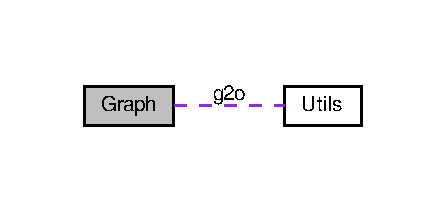
\includegraphics[width=214pt]{group__graph}
\end{center}
\end{figure}


\subsection{详细描述}

\hypertarget{group__g2o}{\section{G2o}
\label{group__g2o}\index{G2o@{G2o}}
}

\hypertarget{group__utils}{\section{Utils}
\label{group__utils}\index{Utils@{Utils}}
}
Utils 的协作图\-:
\nopagebreak
\begin{figure}[H]
\begin{center}
\leavevmode
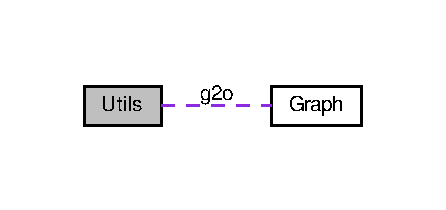
\includegraphics[width=214pt]{group__utils}
\end{center}
\end{figure}
\subsection*{文件}
\begin{DoxyCompactItemize}
\item 
文件 \hyperlink{misc_8h}{misc.\-h}
\begin{DoxyCompactList}\small\item\em some general case utility functions \end{DoxyCompactList}\item 
文件 \hyperlink{timeutil_8h}{timeutil.\-h}
\begin{DoxyCompactList}\small\item\em utility functions for handling time related stuff \end{DoxyCompactList}\end{DoxyCompactItemize}
\subsection*{宏定义}
\begin{DoxyCompactItemize}
\item 
\#define \hyperlink{group__utils_ga9b9f34c01b03b47644c2762bf256be32}{D\-O\-\_\-\-E\-V\-E\-R\-Y\-\_\-\-T\-S}(secs, current\-Time, code)
\item 
\hypertarget{group__utils_gabfe958da8833edbe74250507adc61635}{\#define \hyperlink{group__utils_gabfe958da8833edbe74250507adc61635}{D\-O\-\_\-\-E\-V\-E\-R\-Y}(secs, code)~\hyperlink{group__utils_ga9b9f34c01b03b47644c2762bf256be32}{D\-O\-\_\-\-E\-V\-E\-R\-Y\-\_\-\-T\-S}(secs, g2o\-::get\-\_\-time(), code)}\label{group__utils_gabfe958da8833edbe74250507adc61635}

\begin{DoxyCompactList}\small\item\em Executes code, only if secs are gone since last exec. \end{DoxyCompactList}\item 
\#define {\bfseries M\-E\-A\-S\-U\-R\-E\-\_\-\-T\-I\-M\-E}(text, code)
\item 
\hypertarget{group__utils_gae79acf8eb730f80c029d60e19332b4b9}{\#define {\bfseries M\-E\-A\-S\-U\-R\-E\-\_\-\-F\-U\-N\-C\-T\-I\-O\-N\-\_\-\-T\-I\-M\-E}~\hyperlink{classg2o_1_1ScopeTime}{g2o\-::\-Scope\-Time} scope\-Time(\-\_\-\-\_\-\-P\-R\-E\-T\-T\-Y\-\_\-\-F\-U\-N\-C\-T\-I\-O\-N\-\_\-\-\_\-)}\label{group__utils_gae79acf8eb730f80c029d60e19332b4b9}

\end{DoxyCompactItemize}
\subsection*{函数}
\begin{DoxyCompactItemize}
\item 
std\-::string \hyperlink{group__utils_ga437d185a62afe16a99f27f3b12e108d7}{g2o\-::trim} (const std\-::string \&s)
\item 
std\-::string \hyperlink{group__utils_gad2277aa8d0784f7001f7f27396d59f98}{g2o\-::trim\-Left} (const std\-::string \&s)
\item 
std\-::string \hyperlink{group__utils_ga7305cbf5d345c0e352ac2baa93b7d30a}{g2o\-::trim\-Right} (const std\-::string \&s)
\item 
std\-::string \hyperlink{group__utils_ga18235ef006dc52e266590591f895157d}{g2o\-::str\-To\-Lower} (const std\-::string \&s)
\item 
std\-::string \hyperlink{group__utils_ga70dfb4dd2aeae37635cf2b5bef6321a9}{g2o\-::str\-To\-Upper} (const std\-::string \&s)
\item 
{\footnotesize template$<$typename Output\-Iterator $>$ }\\Output\-Iterator \hyperlink{group__utils_gae501003a8f6b60afb846857fdb82174d}{g2o\-::read\-Ints} (const char $\ast$str, Output\-Iterator out)
\item 
{\footnotesize template$<$typename Output\-Iterator $>$ }\\Output\-Iterator \hyperlink{group__utils_ga88353c6cfc2e519df07814ca577e71ec}{g2o\-::read\-Floats} (const char $\ast$str, Output\-Iterator out)
\item 
std\-::string \hyperlink{group__utils_gadc1d37473e0e8c6a73fb46b19239d2d1}{g2o\-::format\-String} (const char $\ast$fmt,...)
\item 
int \hyperlink{group__utils_gacce5cae59e8c97bf3f4ff581c6534d03}{g2o\-::str\-Printf} (std\-::string \&str, const char $\ast$fmt,...)
\item 
{\footnotesize template$<$typename T $>$ }\\bool \hyperlink{group__utils_ga599c46f6984e9a2147fac39324e9fadc}{g2o\-::convert\-String} (const std\-::string \&s, T \&x, bool fail\-If\-Leftover\-Chars=true)
\item 
{\footnotesize template$<$typename T $>$ }\\T \hyperlink{group__utils_ga9dac39a213d269b8d68fb698bf82873a}{g2o\-::string\-To\-Type} (const std\-::string \&s, bool fail\-If\-Leftover\-Chars=true)
\item 
bool \hyperlink{group__utils_ga98f10a2fabad17ef7ed1534b39eb2bc5}{g2o\-::str\-Starts\-With} (const std\-::string \&s, const std\-::string \&start)
\item 
bool \hyperlink{group__utils_ga7a0e6ad89c4c86b2b60ddf392a57c963}{g2o\-::str\-Ends\-With} (const std\-::string \&s, const std\-::string \&end)
\item 
std\-::string \hyperlink{group__utils_ga45c2648d8a8a5f5bed13741bc8a501d1}{g2o\-::str\-Expand\-Filename} (const std\-::string \&filename)
\item 
std\-::vector$<$ std\-::string $>$ \hyperlink{group__utils_ga0a56de67e98afa3f8307e7b4ddb4cc83}{g2o\-::str\-Split} (const std\-::string \&str, const std\-::string \&delimiters)
\item 
int \hyperlink{group__utils_ga570513203e2bbf23d692460c0aef07e8}{g2o\-::read\-Line} (std\-::istream \&is, std\-::stringstream \&current\-Line)
\end{DoxyCompactItemize}


\subsection{详细描述}


\subsection{宏定义说明}
\hypertarget{group__utils_ga9b9f34c01b03b47644c2762bf256be32}{\index{Utils@{Utils}!D\-O\-\_\-\-E\-V\-E\-R\-Y\-\_\-\-T\-S@{D\-O\-\_\-\-E\-V\-E\-R\-Y\-\_\-\-T\-S}}
\index{D\-O\-\_\-\-E\-V\-E\-R\-Y\-\_\-\-T\-S@{D\-O\-\_\-\-E\-V\-E\-R\-Y\-\_\-\-T\-S}!Utils@{Utils}}
\subsubsection[{D\-O\-\_\-\-E\-V\-E\-R\-Y\-\_\-\-T\-S}]{\setlength{\rightskip}{0pt plus 5cm}\#define D\-O\-\_\-\-E\-V\-E\-R\-Y\-\_\-\-T\-S(
\begin{DoxyParamCaption}
\item[{}]{secs, }
\item[{}]{current\-Time, }
\item[{}]{code}
\end{DoxyParamCaption}
)}}\label{group__utils_ga9b9f34c01b03b47644c2762bf256be32}
{\bfseries 值\-:}
\begin{DoxyCode}
\textcolor{keywordflow}{if} (1) \{\(\backslash\)
  static \textcolor{keywordtype}{double} s\_lastDone\_ = (currentTime); \(\backslash\)
  double s\_now\_ = (currentTime); \(\backslash\)
  if (s\_lastDone\_ > s\_now\_) \(\backslash\)
    s\_lastDone\_ = s\_now\_; \(\backslash\)
  if (s\_now\_ - s\_lastDone\_ > (secs)) \{ \(\backslash\)
    code; \(\backslash\)
    s\_lastDone\_ = s\_now\_; \(\backslash\)
  \}\(\backslash\)
\} \textcolor{keywordflow}{else} \(\backslash\)
  (void)0
\end{DoxyCode}
Executes code, only if secs are gone since last exec. extended version, in which the current time is given, e.\-g., timestamp of I\-P\-C message 

在文件 timeutil.\-h 第 49 行定义.

\hypertarget{group__utils_gaafc27d8d00ac925dce6e52a013cc2b32}{\index{Utils@{Utils}!M\-E\-A\-S\-U\-R\-E\-\_\-\-T\-I\-M\-E@{M\-E\-A\-S\-U\-R\-E\-\_\-\-T\-I\-M\-E}}
\index{M\-E\-A\-S\-U\-R\-E\-\_\-\-T\-I\-M\-E@{M\-E\-A\-S\-U\-R\-E\-\_\-\-T\-I\-M\-E}!Utils@{Utils}}
\subsubsection[{M\-E\-A\-S\-U\-R\-E\-\_\-\-T\-I\-M\-E}]{\setlength{\rightskip}{0pt plus 5cm}\#define M\-E\-A\-S\-U\-R\-E\-\_\-\-T\-I\-M\-E(
\begin{DoxyParamCaption}
\item[{}]{text, }
\item[{}]{code}
\end{DoxyParamCaption}
)}}\label{group__utils_gaafc27d8d00ac925dce6e52a013cc2b32}
{\bfseries 值\-:}
\begin{DoxyCode}
\textcolor{keywordflow}{if}(1) \{ \(\backslash\)
    double \_start\_time\_ = g2o::get\_time(); \(\backslash\)
    code; \(\backslash\)
    fprintf(stderr, \textcolor{stringliteral}{"%s took %f sec\(\backslash\)n"}, text, g2o::get\_time() - \_start\_time\_); \(\backslash\)
  \} \textcolor{keywordflow}{else} \(\backslash\)
    (void) 0
\end{DoxyCode}


在文件 timeutil.\-h 第 69 行定义.



\subsection{函数说明}
\hypertarget{group__utils_ga599c46f6984e9a2147fac39324e9fadc}{\index{Utils@{Utils}!convert\-String@{convert\-String}}
\index{convert\-String@{convert\-String}!Utils@{Utils}}
\subsubsection[{convert\-String}]{\setlength{\rightskip}{0pt plus 5cm}template$<$typename T $>$ bool g2o\-::convert\-String (
\begin{DoxyParamCaption}
\item[{const std\-::string \&}]{s, }
\item[{T \&}]{x, }
\item[{bool}]{fail\-If\-Leftover\-Chars = {\ttfamily true}}
\end{DoxyParamCaption}
)}}\label{group__utils_ga599c46f6984e9a2147fac39324e9fadc}
convert a string into an other type. 

在文件 string\-\_\-tools.\-h 第 125 行定义.



参考自 g2o\-::string\-To\-Type().



这是这个函数的调用关系图\-:
\nopagebreak
\begin{figure}[H]
\begin{center}
\leavevmode
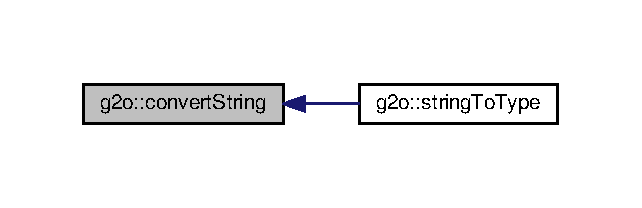
\includegraphics[width=308pt]{group__utils_ga599c46f6984e9a2147fac39324e9fadc_icgraph}
\end{center}
\end{figure}


\hypertarget{group__utils_gadc1d37473e0e8c6a73fb46b19239d2d1}{\index{Utils@{Utils}!format\-String@{format\-String}}
\index{format\-String@{format\-String}!Utils@{Utils}}
\subsubsection[{format\-String}]{\setlength{\rightskip}{0pt plus 5cm}G2\-O\-\_\-\-C\-O\-R\-E\-\_\-\-A\-P\-I std\-::string g2o\-::format\-String (
\begin{DoxyParamCaption}
\item[{const char $\ast$}]{fmt, }
\item[{}]{...}
\end{DoxyParamCaption}
)}}\label{group__utils_gadc1d37473e0e8c6a73fb46b19239d2d1}
format a string and return a std\-::string. Format is just like printf, see man 3 printf 

在文件 string\-\_\-tools.\-cpp 第 95 行定义.

\hypertarget{group__utils_ga88353c6cfc2e519df07814ca577e71ec}{\index{Utils@{Utils}!read\-Floats@{read\-Floats}}
\index{read\-Floats@{read\-Floats}!Utils@{Utils}}
\subsubsection[{read\-Floats}]{\setlength{\rightskip}{0pt plus 5cm}template$<$typename Output\-Iterator $>$ Output\-Iterator g2o\-::read\-Floats (
\begin{DoxyParamCaption}
\item[{const char $\ast$}]{str, }
\item[{Output\-Iterator}]{out}
\end{DoxyParamCaption}
)}}\label{group__utils_ga88353c6cfc2e519df07814ca577e71ec}
read float values (seperated by spaces) from a string and store them in the given Output\-Iterator. 

在文件 string\-\_\-tools.\-h 第 96 行定义.

\hypertarget{group__utils_gae501003a8f6b60afb846857fdb82174d}{\index{Utils@{Utils}!read\-Ints@{read\-Ints}}
\index{read\-Ints@{read\-Ints}!Utils@{Utils}}
\subsubsection[{read\-Ints}]{\setlength{\rightskip}{0pt plus 5cm}template$<$typename Output\-Iterator $>$ Output\-Iterator g2o\-::read\-Ints (
\begin{DoxyParamCaption}
\item[{const char $\ast$}]{str, }
\item[{Output\-Iterator}]{out}
\end{DoxyParamCaption}
)}}\label{group__utils_gae501003a8f6b60afb846857fdb82174d}
read integer values (seperated by spaces) from a string and store them in the given Output\-Iterator. 

在文件 string\-\_\-tools.\-h 第 77 行定义.

\hypertarget{group__utils_ga570513203e2bbf23d692460c0aef07e8}{\index{Utils@{Utils}!read\-Line@{read\-Line}}
\index{read\-Line@{read\-Line}!Utils@{Utils}}
\subsubsection[{read\-Line}]{\setlength{\rightskip}{0pt plus 5cm}G2\-O\-\_\-\-C\-O\-R\-E\-\_\-\-A\-P\-I int g2o\-::read\-Line (
\begin{DoxyParamCaption}
\item[{std\-::istream \&}]{is, }
\item[{std\-::stringstream \&}]{current\-Line}
\end{DoxyParamCaption}
)}}\label{group__utils_ga570513203e2bbf23d692460c0aef07e8}
read a line from is into current\-Line. \begin{DoxyReturn}{返回}
the number of characters read into current\-Line (excluding newline), -\/1 on eof() 
\end{DoxyReturn}


在文件 string\-\_\-tools.\-cpp 第 172 行定义.



参考自 g2o\-::\-Parameter\-Container\-::read().



这是这个函数的调用关系图\-:
\nopagebreak
\begin{figure}[H]
\begin{center}
\leavevmode
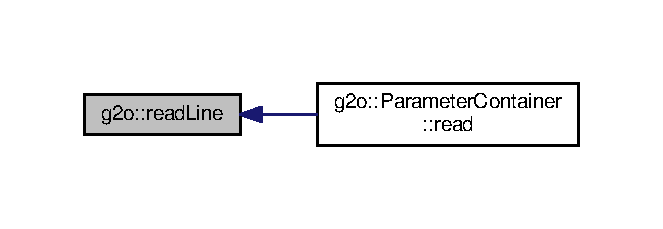
\includegraphics[width=318pt]{group__utils_ga570513203e2bbf23d692460c0aef07e8_icgraph}
\end{center}
\end{figure}


\hypertarget{group__utils_ga7a0e6ad89c4c86b2b60ddf392a57c963}{\index{Utils@{Utils}!str\-Ends\-With@{str\-Ends\-With}}
\index{str\-Ends\-With@{str\-Ends\-With}!Utils@{Utils}}
\subsubsection[{str\-Ends\-With}]{\setlength{\rightskip}{0pt plus 5cm}G2\-O\-\_\-\-C\-O\-R\-E\-\_\-\-A\-P\-I bool g2o\-::str\-Ends\-With (
\begin{DoxyParamCaption}
\item[{const std\-::string \&}]{str, }
\item[{const std\-::string \&}]{substr}
\end{DoxyParamCaption}
)}}\label{group__utils_ga7a0e6ad89c4c86b2b60ddf392a57c963}
return true, if str ends with substr 

在文件 string\-\_\-tools.\-cpp 第 165 行定义.

\hypertarget{group__utils_ga45c2648d8a8a5f5bed13741bc8a501d1}{\index{Utils@{Utils}!str\-Expand\-Filename@{str\-Expand\-Filename}}
\index{str\-Expand\-Filename@{str\-Expand\-Filename}!Utils@{Utils}}
\subsubsection[{str\-Expand\-Filename}]{\setlength{\rightskip}{0pt plus 5cm}G2\-O\-\_\-\-C\-O\-R\-E\-\_\-\-A\-P\-I std\-::string g2o\-::str\-Expand\-Filename (
\begin{DoxyParamCaption}
\item[{const std\-::string \&}]{filename}
\end{DoxyParamCaption}
)}}\label{group__utils_ga45c2648d8a8a5f5bed13741bc8a501d1}
expand the given filename like a posix shell, e.\-g., $\sim$ \$\-C\-A\-R\-M\-E\-N\-\_\-\-H\-O\-M\-E and other will get expanded. Also command substitution, e.\-g. {\ttfamily pwd} will give the current directory. 

在文件 string\-\_\-tools.\-cpp 第 124 行定义.

\hypertarget{group__utils_ga9dac39a213d269b8d68fb698bf82873a}{\index{Utils@{Utils}!string\-To\-Type@{string\-To\-Type}}
\index{string\-To\-Type@{string\-To\-Type}!Utils@{Utils}}
\subsubsection[{string\-To\-Type}]{\setlength{\rightskip}{0pt plus 5cm}template$<$typename T $>$ T g2o\-::string\-To\-Type (
\begin{DoxyParamCaption}
\item[{const std\-::string \&}]{s, }
\item[{bool}]{fail\-If\-Leftover\-Chars = {\ttfamily true}}
\end{DoxyParamCaption}
)}}\label{group__utils_ga9dac39a213d269b8d68fb698bf82873a}
convert a string into an other type. Return the converted value. Throw error if parsing is wrong. 

在文件 string\-\_\-tools.\-h 第 139 行定义.



参考 g2o\-::convert\-String().



函数调用图\-:
\nopagebreak
\begin{figure}[H]
\begin{center}
\leavevmode
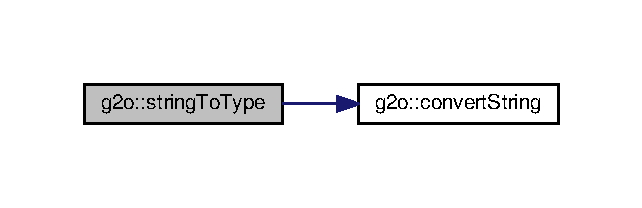
\includegraphics[width=308pt]{group__utils_ga9dac39a213d269b8d68fb698bf82873a_cgraph}
\end{center}
\end{figure}


\hypertarget{group__utils_gacce5cae59e8c97bf3f4ff581c6534d03}{\index{Utils@{Utils}!str\-Printf@{str\-Printf}}
\index{str\-Printf@{str\-Printf}!Utils@{Utils}}
\subsubsection[{str\-Printf}]{\setlength{\rightskip}{0pt plus 5cm}G2\-O\-\_\-\-C\-O\-R\-E\-\_\-\-A\-P\-I int g2o\-::str\-Printf (
\begin{DoxyParamCaption}
\item[{std\-::string \&}]{str, }
\item[{const char $\ast$}]{fmt, }
\item[{}]{...}
\end{DoxyParamCaption}
)}}\label{group__utils_gacce5cae59e8c97bf3f4ff581c6534d03}
replacement function for sprintf which fills a std\-::string instead of a char$\ast$ 

在文件 string\-\_\-tools.\-cpp 第 112 行定义.

\hypertarget{group__utils_ga0a56de67e98afa3f8307e7b4ddb4cc83}{\index{Utils@{Utils}!str\-Split@{str\-Split}}
\index{str\-Split@{str\-Split}!Utils@{Utils}}
\subsubsection[{str\-Split}]{\setlength{\rightskip}{0pt plus 5cm}G2\-O\-\_\-\-C\-O\-R\-E\-\_\-\-A\-P\-I std\-::vector$<$ std\-::string $>$ g2o\-::str\-Split (
\begin{DoxyParamCaption}
\item[{const std\-::string \&}]{s, }
\item[{const std\-::string \&}]{delim}
\end{DoxyParamCaption}
)}}\label{group__utils_ga0a56de67e98afa3f8307e7b4ddb4cc83}
split a string into token based on the characters given in delim 

在文件 string\-\_\-tools.\-cpp 第 143 行定义.



参考自 g2o\-::\-Optimizable\-Graph\-::set\-Renamed\-Types\-From\-String() , 以及 g2o\-::\-Property\-Map\-::update\-Map\-From\-String().



这是这个函数的调用关系图\-:
\nopagebreak
\begin{figure}[H]
\begin{center}
\leavevmode
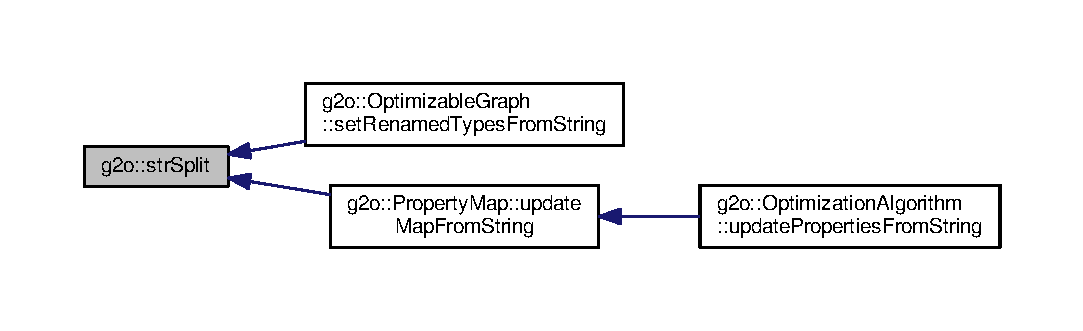
\includegraphics[width=350pt]{group__utils_ga0a56de67e98afa3f8307e7b4ddb4cc83_icgraph}
\end{center}
\end{figure}


\hypertarget{group__utils_ga98f10a2fabad17ef7ed1534b39eb2bc5}{\index{Utils@{Utils}!str\-Starts\-With@{str\-Starts\-With}}
\index{str\-Starts\-With@{str\-Starts\-With}!Utils@{Utils}}
\subsubsection[{str\-Starts\-With}]{\setlength{\rightskip}{0pt plus 5cm}G2\-O\-\_\-\-C\-O\-R\-E\-\_\-\-A\-P\-I bool g2o\-::str\-Starts\-With (
\begin{DoxyParamCaption}
\item[{const std\-::string \&}]{str, }
\item[{const std\-::string \&}]{substr}
\end{DoxyParamCaption}
)}}\label{group__utils_ga98f10a2fabad17ef7ed1534b39eb2bc5}
return true, if str starts with substr 

在文件 string\-\_\-tools.\-cpp 第 158 行定义.

\hypertarget{group__utils_ga18235ef006dc52e266590591f895157d}{\index{Utils@{Utils}!str\-To\-Lower@{str\-To\-Lower}}
\index{str\-To\-Lower@{str\-To\-Lower}!Utils@{Utils}}
\subsubsection[{str\-To\-Lower}]{\setlength{\rightskip}{0pt plus 5cm}G2\-O\-\_\-\-C\-O\-R\-E\-\_\-\-A\-P\-I std\-::string g2o\-::str\-To\-Lower (
\begin{DoxyParamCaption}
\item[{const std\-::string \&}]{s}
\end{DoxyParamCaption}
)}}\label{group__utils_ga18235ef006dc52e266590591f895157d}
convert the string to lower case 

在文件 string\-\_\-tools.\-cpp 第 81 行定义.

\hypertarget{group__utils_ga70dfb4dd2aeae37635cf2b5bef6321a9}{\index{Utils@{Utils}!str\-To\-Upper@{str\-To\-Upper}}
\index{str\-To\-Upper@{str\-To\-Upper}!Utils@{Utils}}
\subsubsection[{str\-To\-Upper}]{\setlength{\rightskip}{0pt plus 5cm}G2\-O\-\_\-\-C\-O\-R\-E\-\_\-\-A\-P\-I std\-::string g2o\-::str\-To\-Upper (
\begin{DoxyParamCaption}
\item[{const std\-::string \&}]{s}
\end{DoxyParamCaption}
)}}\label{group__utils_ga70dfb4dd2aeae37635cf2b5bef6321a9}
convert a string to upper case 

在文件 string\-\_\-tools.\-cpp 第 88 行定义.

\hypertarget{group__utils_ga437d185a62afe16a99f27f3b12e108d7}{\index{Utils@{Utils}!trim@{trim}}
\index{trim@{trim}!Utils@{Utils}}
\subsubsection[{trim}]{\setlength{\rightskip}{0pt plus 5cm}G2\-O\-\_\-\-C\-O\-R\-E\-\_\-\-A\-P\-I std\-::string g2o\-::trim (
\begin{DoxyParamCaption}
\item[{const std\-::string \&}]{s}
\end{DoxyParamCaption}
)}}\label{group__utils_ga437d185a62afe16a99f27f3b12e108d7}
remove whitespaces from the start/end of a string 

在文件 string\-\_\-tools.\-cpp 第 48 行定义.



参考自 g2o\-::\-Optimizable\-Graph\-::set\-Renamed\-Types\-From\-String() , 以及 g2o\-::\-Property\-Map\-::update\-Map\-From\-String().



这是这个函数的调用关系图\-:
\nopagebreak
\begin{figure}[H]
\begin{center}
\leavevmode
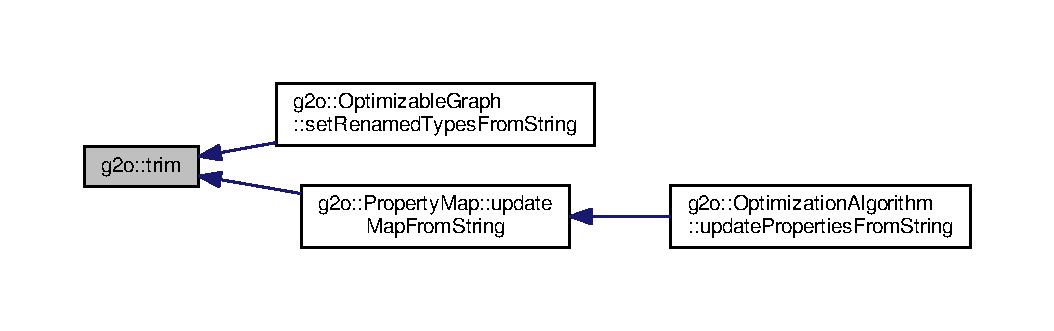
\includegraphics[width=350pt]{group__utils_ga437d185a62afe16a99f27f3b12e108d7_icgraph}
\end{center}
\end{figure}


\hypertarget{group__utils_gad2277aa8d0784f7001f7f27396d59f98}{\index{Utils@{Utils}!trim\-Left@{trim\-Left}}
\index{trim\-Left@{trim\-Left}!Utils@{Utils}}
\subsubsection[{trim\-Left}]{\setlength{\rightskip}{0pt plus 5cm}G2\-O\-\_\-\-C\-O\-R\-E\-\_\-\-A\-P\-I std\-::string g2o\-::trim\-Left (
\begin{DoxyParamCaption}
\item[{const std\-::string \&}]{s}
\end{DoxyParamCaption}
)}}\label{group__utils_gad2277aa8d0784f7001f7f27396d59f98}
remove whitespaces from the left side of the string 

在文件 string\-\_\-tools.\-cpp 第 59 行定义.

\hypertarget{group__utils_ga7305cbf5d345c0e352ac2baa93b7d30a}{\index{Utils@{Utils}!trim\-Right@{trim\-Right}}
\index{trim\-Right@{trim\-Right}!Utils@{Utils}}
\subsubsection[{trim\-Right}]{\setlength{\rightskip}{0pt plus 5cm}G2\-O\-\_\-\-C\-O\-R\-E\-\_\-\-A\-P\-I std\-::string g2o\-::trim\-Right (
\begin{DoxyParamCaption}
\item[{const std\-::string \&}]{s}
\end{DoxyParamCaption}
)}}\label{group__utils_ga7305cbf5d345c0e352ac2baa93b7d30a}
remove whitespaced from the right side of the string 

在文件 string\-\_\-tools.\-cpp 第 70 行定义.


\chapter{命名空间文档}
\hypertarget{namespaceDBoW2}{\section{D\-Bo\-W2 命名空间参考}
\label{namespaceDBoW2}\index{D\-Bo\-W2@{D\-Bo\-W2}}
}
\subsection*{类}
\begin{DoxyCompactItemize}
\item 
class \hyperlink{classDBoW2_1_1BowVector}{Bow\-Vector}
\item 
class \hyperlink{classDBoW2_1_1FClass}{F\-Class}
\begin{DoxyCompactList}\small\item\em Generic class to encapsulate functions to manage descriptors. \end{DoxyCompactList}\item 
class \hyperlink{classDBoW2_1_1FeatureVector}{Feature\-Vector}
\begin{DoxyCompactList}\small\item\em Vector of nodes with indexes of local features。正索引,node,对应的特征的标号 \end{DoxyCompactList}\item 
class \hyperlink{classDBoW2_1_1FORB}{F\-O\-R\-B}
\begin{DoxyCompactList}\small\item\em Functions to manipulate O\-R\-B descriptors. \end{DoxyCompactList}\item 
class \hyperlink{classDBoW2_1_1GeneralScoring}{General\-Scoring}
\begin{DoxyCompactList}\small\item\em Base class of scoring functions. \end{DoxyCompactList}\item 
class \hyperlink{classDBoW2_1_1TemplatedVocabulary}{Templated\-Vocabulary}
\begin{DoxyCompactList}\small\item\em Generic Vocabulary. \end{DoxyCompactList}\end{DoxyCompactItemize}
\subsection*{类型定义}
\begin{DoxyCompactItemize}
\item 
\hypertarget{namespaceDBoW2_ab1a0d3283b2d4690a383372ed20bfeb5}{typedef unsigned int \hyperlink{namespaceDBoW2_ab1a0d3283b2d4690a383372ed20bfeb5}{Word\-Id}}\label{namespaceDBoW2_ab1a0d3283b2d4690a383372ed20bfeb5}

\begin{DoxyCompactList}\small\item\em Id of words. \end{DoxyCompactList}\item 
\hypertarget{namespaceDBoW2_a55fcd7333e591a38e96b91f41bc182f6}{typedef double \hyperlink{namespaceDBoW2_a55fcd7333e591a38e96b91f41bc182f6}{Word\-Value}}\label{namespaceDBoW2_a55fcd7333e591a38e96b91f41bc182f6}

\begin{DoxyCompactList}\small\item\em Value of a word. \end{DoxyCompactList}\item 
\hypertarget{namespaceDBoW2_a3a0fa9c50c0df508759362d6204566f2}{typedef unsigned int \hyperlink{namespaceDBoW2_a3a0fa9c50c0df508759362d6204566f2}{Node\-Id}}\label{namespaceDBoW2_a3a0fa9c50c0df508759362d6204566f2}

\begin{DoxyCompactList}\small\item\em Id of nodes in the vocabulary treee. \end{DoxyCompactList}\item 
\hypertarget{namespaceDBoW2_a350a8bb9e38231cbf68ef07399d7a0c8}{typedef E\-X\-P\-O\-R\-T enum \hyperlink{namespaceDBoW2_a53e9e0bcfc25c861815e413a7cf3fa51}{D\-Bo\-W2\-::\-L\-Norm} \hyperlink{namespaceDBoW2_a350a8bb9e38231cbf68ef07399d7a0c8}{L\-Norm}}\label{namespaceDBoW2_a350a8bb9e38231cbf68ef07399d7a0c8}

\begin{DoxyCompactList}\small\item\em L-\/norms for normalization. \end{DoxyCompactList}\item 
\hypertarget{namespaceDBoW2_a66be5c3cd2567ff15eeaf56fd55fffcc}{typedef E\-X\-P\-O\-R\-T enum \\*
\hyperlink{namespaceDBoW2_a5de5c8a307aca9a84ffefda2a9bc467a}{D\-Bo\-W2\-::\-Weighting\-Type} \hyperlink{namespaceDBoW2_a66be5c3cd2567ff15eeaf56fd55fffcc}{Weighting\-Type}}\label{namespaceDBoW2_a66be5c3cd2567ff15eeaf56fd55fffcc}

\begin{DoxyCompactList}\small\item\em Weighting type. \end{DoxyCompactList}\item 
\hypertarget{namespaceDBoW2_ad047d6578eacc8aaae7d9cbcd3ded537}{typedef E\-X\-P\-O\-R\-T enum \\*
\hyperlink{namespaceDBoW2_aa252a592dd607c6e60dede06ceef2722}{D\-Bo\-W2\-::\-Scoring\-Type} \hyperlink{namespaceDBoW2_ad047d6578eacc8aaae7d9cbcd3ded537}{Scoring\-Type}}\label{namespaceDBoW2_ad047d6578eacc8aaae7d9cbcd3ded537}

\begin{DoxyCompactList}\small\item\em Scoring type. \end{DoxyCompactList}\end{DoxyCompactItemize}
\subsection*{枚举}
\begin{DoxyCompactItemize}
\item 
enum \hyperlink{namespaceDBoW2_a53e9e0bcfc25c861815e413a7cf3fa51}{L\-Norm} \{ {\bfseries L1}, 
{\bfseries L2}
 \}
\begin{DoxyCompactList}\small\item\em L-\/norms for normalization. \end{DoxyCompactList}\item 
enum \hyperlink{namespaceDBoW2_a5de5c8a307aca9a84ffefda2a9bc467a}{Weighting\-Type} \{ {\bfseries T\-F\-\_\-\-I\-D\-F}, 
{\bfseries T\-F}, 
{\bfseries I\-D\-F}, 
{\bfseries B\-I\-N\-A\-R\-Y}
 \}
\begin{DoxyCompactList}\small\item\em Weighting type. \end{DoxyCompactList}\item 
enum \hyperlink{namespaceDBoW2_aa252a592dd607c6e60dede06ceef2722}{Scoring\-Type} \{ \\*
{\bfseries L1\-\_\-\-N\-O\-R\-M}, 
{\bfseries L2\-\_\-\-N\-O\-R\-M}, 
{\bfseries C\-H\-I\-\_\-\-S\-Q\-U\-A\-R\-E}, 
{\bfseries K\-L}, 
\\*
{\bfseries B\-H\-A\-T\-T\-A\-C\-H\-A\-R\-Y\-Y\-A}, 
{\bfseries D\-O\-T\-\_\-\-P\-R\-O\-D\-U\-C\-T}
 \}
\begin{DoxyCompactList}\small\item\em Scoring type. \end{DoxyCompactList}\end{DoxyCompactItemize}
\subsection*{函数}
\begin{DoxyCompactItemize}
\item 
std\-::ostream \& \hyperlink{namespaceDBoW2_a06d2058b1bde1cdc49f277fec62073e2}{operator$<$$<$} (std\-::ostream \&out, const \hyperlink{classDBoW2_1_1BowVector}{Bow\-Vector} \&v)
\item 
std\-::ostream \& \hyperlink{namespaceDBoW2_ac65e2bfb945a77c5294d0300a4fed49c}{operator$<$$<$} (std\-::ostream \&out, const \hyperlink{classDBoW2_1_1FeatureVector}{Feature\-Vector} \&v)
\item 
\hypertarget{namespaceDBoW2_a366d1d4a75ab8276e171af0aaa04b29b}{class E\-X\-P\-O\-R\-T \hyperlink{namespaceDBoW2_a366d1d4a75ab8276e171af0aaa04b29b}{\-\_\-\-\_\-\-S\-C\-O\-R\-I\-N\-G\-\_\-\-C\-L\-A\-S\-S} (L1\-Scoring, true, L1)}\label{namespaceDBoW2_a366d1d4a75ab8276e171af0aaa04b29b}

\begin{DoxyCompactList}\small\item\em L1 Scoring object. \end{DoxyCompactList}\item 
\hypertarget{namespaceDBoW2_a38216a543c4968d22bf2ffd2178e299c}{class E\-X\-P\-O\-R\-T \hyperlink{namespaceDBoW2_a38216a543c4968d22bf2ffd2178e299c}{\-\_\-\-\_\-\-S\-C\-O\-R\-I\-N\-G\-\_\-\-C\-L\-A\-S\-S} (L2\-Scoring, true, L2)}\label{namespaceDBoW2_a38216a543c4968d22bf2ffd2178e299c}

\begin{DoxyCompactList}\small\item\em L2 Scoring object. \end{DoxyCompactList}\item 
\hypertarget{namespaceDBoW2_adc330022cadf004b7ed5b84203287039}{class E\-X\-P\-O\-R\-T \hyperlink{namespaceDBoW2_adc330022cadf004b7ed5b84203287039}{\-\_\-\-\_\-\-S\-C\-O\-R\-I\-N\-G\-\_\-\-C\-L\-A\-S\-S} (Chi\-Square\-Scoring, true, L1)}\label{namespaceDBoW2_adc330022cadf004b7ed5b84203287039}

\begin{DoxyCompactList}\small\item\em Chi square Scoring object. \end{DoxyCompactList}\item 
\hypertarget{namespaceDBoW2_a9af1c21239089d77c337c65fac3e7bf5}{class E\-X\-P\-O\-R\-T \hyperlink{namespaceDBoW2_a9af1c21239089d77c337c65fac3e7bf5}{\-\_\-\-\_\-\-S\-C\-O\-R\-I\-N\-G\-\_\-\-C\-L\-A\-S\-S} (K\-L\-Scoring, true, L1)}\label{namespaceDBoW2_a9af1c21239089d77c337c65fac3e7bf5}

\begin{DoxyCompactList}\small\item\em K\-L divergence Scoring object. \end{DoxyCompactList}\item 
\hypertarget{namespaceDBoW2_a7135fab6a887afb7d2b4e6254b4875ea}{class E\-X\-P\-O\-R\-T \hyperlink{namespaceDBoW2_a7135fab6a887afb7d2b4e6254b4875ea}{\-\_\-\-\_\-\-S\-C\-O\-R\-I\-N\-G\-\_\-\-C\-L\-A\-S\-S} (Bhattacharyya\-Scoring, true, L1)}\label{namespaceDBoW2_a7135fab6a887afb7d2b4e6254b4875ea}

\begin{DoxyCompactList}\small\item\em Bhattacharyya Scoring object. \end{DoxyCompactList}\item 
\hypertarget{namespaceDBoW2_a8b3715c76bccab82aa18804b6b7dc1ba}{class E\-X\-P\-O\-R\-T \hyperlink{namespaceDBoW2_a8b3715c76bccab82aa18804b6b7dc1ba}{\-\_\-\-\_\-\-S\-C\-O\-R\-I\-N\-G\-\_\-\-C\-L\-A\-S\-S} (Dot\-Product\-Scoring, false, L1)}\label{namespaceDBoW2_a8b3715c76bccab82aa18804b6b7dc1ba}

\begin{DoxyCompactList}\small\item\em Dot product Scoring object. \end{DoxyCompactList}\item 
{\footnotesize template$<$class T\-Descriptor , class F $>$ }\\std\-::ostream \& \hyperlink{namespaceDBoW2_aecdf616fe16d2cf09f521a603b9d43f1}{operator$<$$<$} (std\-::ostream \&os, const \hyperlink{classDBoW2_1_1TemplatedVocabulary}{Templated\-Vocabulary}$<$ T\-Descriptor, F $>$ \&voc)
\end{DoxyCompactItemize}


\subsection{详细描述}
File\-: \hyperlink{BowVector_8cpp_source}{Bow\-Vector.\-cpp} Date\-: March 2011 Author\-: Dorian Galvez-\/\-Lopez Description\-: bag of words vector License\-: see the L\-I\-C\-E\-N\-S\-E.\-txt file

File\-: \hyperlink{BowVector_8h_source}{Bow\-Vector.\-h} Date\-: March 2011 Author\-: Dorian Galvez-\/\-Lopez Description\-: bag of words vector License\-: see the L\-I\-C\-E\-N\-S\-E.\-txt file

File\-: \hyperlink{FClass_8h_source}{F\-Class.\-h} Date\-: November 2011 Author\-: Dorian Galvez-\/\-Lopez Description\-: generic \hyperlink{classDBoW2_1_1FClass}{F\-Class} to instantiate templated classes License\-: see the L\-I\-C\-E\-N\-S\-E.\-txt file

File\-: \hyperlink{FeatureVector_8cpp_source}{Feature\-Vector.\-cpp} Date\-: November 2011 Author\-: Dorian Galvez-\/\-Lopez Description\-: feature vector License\-: see the L\-I\-C\-E\-N\-S\-E.\-txt file

File\-: \hyperlink{FeatureVector_8h_source}{Feature\-Vector.\-h} Date\-: November 2011 Author\-: Dorian Galvez-\/\-Lopez Description\-: feature vector License\-: see the L\-I\-C\-E\-N\-S\-E.\-txt file

File\-: \hyperlink{FORB_8h_source}{F\-O\-R\-B.\-h} Date\-: June 2012 Author\-: Dorian Galvez-\/\-Lopez Description\-: functions for O\-R\-B descriptors License\-: see the L\-I\-C\-E\-N\-S\-E.\-txt file

File\-: \hyperlink{ScoringObject_8h_source}{Scoring\-Object.\-h} Date\-: November 2011 Author\-: Dorian Galvez-\/\-Lopez Description\-: functions to compute bow scores License\-: see the L\-I\-C\-E\-N\-S\-E.\-txt file 

\subsection{函数说明}
\hypertarget{namespaceDBoW2_ac65e2bfb945a77c5294d0300a4fed49c}{\index{D\-Bo\-W2@{D\-Bo\-W2}!operator$<$$<$@{operator$<$$<$}}
\index{operator$<$$<$@{operator$<$$<$}!DBoW2@{D\-Bo\-W2}}
\subsubsection[{operator$<$$<$}]{\setlength{\rightskip}{0pt plus 5cm}std\-::ostream\& D\-Bo\-W2\-::operator$<$$<$ (
\begin{DoxyParamCaption}
\item[{std\-::ostream \&}]{out, }
\item[{const Feature\-Vector \&}]{v}
\end{DoxyParamCaption}
)}}\label{namespaceDBoW2_ac65e2bfb945a77c5294d0300a4fed49c}
Sends a string versions of the feature vector through the stream 
\begin{DoxyParams}{参数}
{\em out} & stream \\
\hline
{\em v} & feature vector \\
\hline
\end{DoxyParams}


在文件 Feature\-Vector.\-cpp 第 49 行定义.

\hypertarget{namespaceDBoW2_a06d2058b1bde1cdc49f277fec62073e2}{\index{D\-Bo\-W2@{D\-Bo\-W2}!operator$<$$<$@{operator$<$$<$}}
\index{operator$<$$<$@{operator$<$$<$}!DBoW2@{D\-Bo\-W2}}
\subsubsection[{operator$<$$<$}]{\setlength{\rightskip}{0pt plus 5cm}std\-::ostream\& D\-Bo\-W2\-::operator$<$$<$ (
\begin{DoxyParamCaption}
\item[{std\-::ostream \&}]{out, }
\item[{const Bow\-Vector \&}]{v}
\end{DoxyParamCaption}
)}}\label{namespaceDBoW2_a06d2058b1bde1cdc49f277fec62073e2}
Prints the content of the bow vector 
\begin{DoxyParams}{参数}
{\em out} & stream \\
\hline
{\em v} & \\
\hline
\end{DoxyParams}


在文件 Bow\-Vector.\-cpp 第 88 行定义.

\hypertarget{namespaceDBoW2_aecdf616fe16d2cf09f521a603b9d43f1}{\index{D\-Bo\-W2@{D\-Bo\-W2}!operator$<$$<$@{operator$<$$<$}}
\index{operator$<$$<$@{operator$<$$<$}!DBoW2@{D\-Bo\-W2}}
\subsubsection[{operator$<$$<$}]{\setlength{\rightskip}{0pt plus 5cm}template$<$class T\-Descriptor , class F $>$ std\-::ostream\& D\-Bo\-W2\-::operator$<$$<$ (
\begin{DoxyParamCaption}
\item[{std\-::ostream \&}]{os, }
\item[{const Templated\-Vocabulary$<$ T\-Descriptor, F $>$ \&}]{voc}
\end{DoxyParamCaption}
)}}\label{namespaceDBoW2_aecdf616fe16d2cf09f521a603b9d43f1}
Writes printable information of the vocabulary 
\begin{DoxyParams}{参数}
{\em os} & stream to write to \\
\hline
{\em voc} & \\
\hline
\end{DoxyParams}


在文件 Templated\-Vocabulary.\-h 第 1731 行定义.



参考 D\-Bo\-W2\-::\-Templated\-Vocabulary$<$ T\-Descriptor, F $>$\-::get\-Branching\-Factor(), D\-Bo\-W2\-::\-Templated\-Vocabulary$<$ T\-Descriptor, F $>$\-::get\-Depth\-Levels(), D\-Bo\-W2\-::\-Templated\-Vocabulary$<$ T\-Descriptor, F $>$\-::get\-Scoring\-Type(), D\-Bo\-W2\-::\-Templated\-Vocabulary$<$ T\-Descriptor, F $>$\-::get\-Weighting\-Type() , 以及 D\-Bo\-W2\-::\-Templated\-Vocabulary$<$ T\-Descriptor, F $>$\-::size().



函数调用图\-:
\nopagebreak
\begin{figure}[H]
\begin{center}
\leavevmode
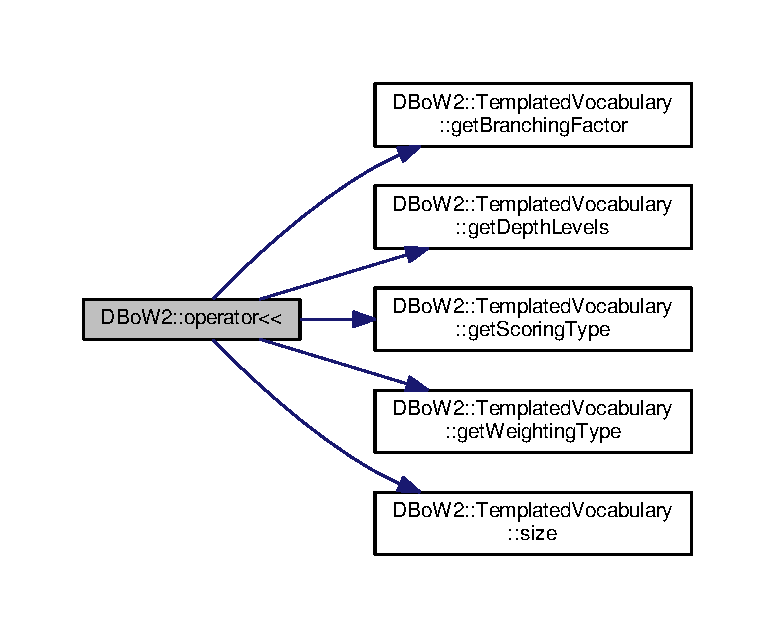
\includegraphics[width=350pt]{namespaceDBoW2_aecdf616fe16d2cf09f521a603b9d43f1_cgraph}
\end{center}
\end{figure}



\hypertarget{namespaceORB__SLAM2}{\section{O\-R\-B\-\_\-\-S\-L\-A\-M2 命名空间参考}
\label{namespaceORB__SLAM2}\index{O\-R\-B\-\_\-\-S\-L\-A\-M2@{O\-R\-B\-\_\-\-S\-L\-A\-M2}}
}
\subsection*{类}
\begin{DoxyCompactItemize}
\item 
class \hyperlink{classORB__SLAM2_1_1Converter}{Converter}
\begin{DoxyCompactList}\small\item\em 提供了一些常见的转换 \end{DoxyCompactList}\item 
class \hyperlink{classORB__SLAM2_1_1Frame}{Frame}
\item 
class \hyperlink{classORB__SLAM2_1_1FrameDrawer}{Frame\-Drawer}
\item 
class \hyperlink{classORB__SLAM2_1_1Initializer}{Initializer}
\begin{DoxyCompactList}\small\item\em 单目\-S\-L\-A\-M初始化相关,双目和\-R\-G\-B\-D不会使用这个类 \end{DoxyCompactList}\item 
class \hyperlink{classORB__SLAM2_1_1KeyFrame}{Key\-Frame}
\item 
class \hyperlink{classORB__SLAM2_1_1KeyFrameDatabase}{Key\-Frame\-Database}
\item 
class \hyperlink{classORB__SLAM2_1_1LocalMapping}{Local\-Mapping}
\item 
class \hyperlink{classORB__SLAM2_1_1LoopClosing}{Loop\-Closing}
\item 
class \hyperlink{classORB__SLAM2_1_1Map}{Map}
\item 
class \hyperlink{classORB__SLAM2_1_1MapDrawer}{Map\-Drawer}
\item 
class \hyperlink{classORB__SLAM2_1_1MapPoint}{Map\-Point}
\begin{DoxyCompactList}\small\item\em Map\-Point是一个地图点 \end{DoxyCompactList}\item 
class \hyperlink{classORB__SLAM2_1_1Optimizer}{Optimizer}
\item 
class \hyperlink{classORB__SLAM2_1_1ExtractorNode}{Extractor\-Node}
\item 
class \hyperlink{classORB__SLAM2_1_1ORBextractor}{O\-R\-Bextractor}
\item 
class \hyperlink{classORB__SLAM2_1_1ORBmatcher}{O\-R\-Bmatcher}
\item 
class \hyperlink{classORB__SLAM2_1_1PnPsolver}{Pn\-Psolver}
\item 
class \hyperlink{classORB__SLAM2_1_1Sim3Solver}{Sim3\-Solver}
\item 
class \hyperlink{classORB__SLAM2_1_1System}{System}
\item 
class \hyperlink{classORB__SLAM2_1_1Tracking}{Tracking}
\item 
class \hyperlink{classORB__SLAM2_1_1Viewer}{Viewer}
\end{DoxyCompactItemize}
\subsection*{类型定义}
\begin{DoxyCompactItemize}
\item 
\hypertarget{namespaceORB__SLAM2_a2fafba714858cab1bb18d438e2e83c5d}{typedef \\*
\hyperlink{classDBoW2_1_1TemplatedVocabulary}{D\-Bo\-W2\-::\-Templated\-Vocabulary}\\*
$<$ \hyperlink{classDBoW2_1_1FORB_aef9b966d0293836fab9f55f1799ce0ed}{D\-Bo\-W2\-::\-F\-O\-R\-B\-::\-T\-Descriptor}, \\*
\hyperlink{classDBoW2_1_1FORB}{D\-Bo\-W2\-::\-F\-O\-R\-B} $>$ {\bfseries O\-R\-B\-Vocabulary}}\label{namespaceORB__SLAM2_a2fafba714858cab1bb18d438e2e83c5d}

\end{DoxyCompactItemize}
\subsection*{变量}
\begin{DoxyCompactItemize}
\item 
\hypertarget{namespaceORB__SLAM2_a557e5c298c5f7164667f083494c2197a}{const int {\bfseries P\-A\-T\-C\-H\-\_\-\-S\-I\-Z\-E} = 31}\label{namespaceORB__SLAM2_a557e5c298c5f7164667f083494c2197a}

\item 
\hypertarget{namespaceORB__SLAM2_aa09849ae679bf2392b097abd710d8d7f}{const int {\bfseries H\-A\-L\-F\-\_\-\-P\-A\-T\-C\-H\-\_\-\-S\-I\-Z\-E} = 15}\label{namespaceORB__SLAM2_aa09849ae679bf2392b097abd710d8d7f}

\item 
\hypertarget{namespaceORB__SLAM2_aec00f1ad4dea35755e3af4404282cd3b}{const int {\bfseries E\-D\-G\-E\-\_\-\-T\-H\-R\-E\-S\-H\-O\-L\-D} = 19}\label{namespaceORB__SLAM2_aec00f1ad4dea35755e3af4404282cd3b}

\item 
\hypertarget{namespaceORB__SLAM2_a8015b470ffeb885a0c90837a03b3210f}{const float {\bfseries factor\-P\-I} = (float)(C\-V\-\_\-\-P\-I/180.f)}\label{namespaceORB__SLAM2_a8015b470ffeb885a0c90837a03b3210f}

\end{DoxyCompactItemize}


\subsection{详细描述}
This file is part of O\-R\-B-\/\-S\-L\-A\-M2.

Copyright (C) 2014-\/2016 Raúl Mur-\/\-Artal $<$raulmur at=\char`\"{}\char`\"{} unizar=\char`\"{}\char`\"{} dot=\char`\"{}\char`\"{} es$>$=\char`\"{}\char`\"{}$>$ (University of Zaragoza) For more information see \href{https://github.com/raulmur/ORB_SLAM2}{\tt https\-://github.\-com/raulmur/\-O\-R\-B\-\_\-\-S\-L\-A\-M2}

O\-R\-B-\/\-S\-L\-A\-M2 is free software\-: you can redistribute it and/or modify it under the terms of the G\-N\-U General Public License as published by the Free Software Foundation, either version 3 of the License, or (at your option) any later version.

O\-R\-B-\/\-S\-L\-A\-M2 is distributed in the hope that it will be useful, but W\-I\-T\-H\-O\-U\-T A\-N\-Y W\-A\-R\-R\-A\-N\-T\-Y; without even the implied warranty of M\-E\-R\-C\-H\-A\-N\-T\-A\-B\-I\-L\-I\-T\-Y or F\-I\-T\-N\-E\-S\-S F\-O\-R A P\-A\-R\-T\-I\-C\-U\-L\-A\-R P\-U\-R\-P\-O\-S\-E. See the G\-N\-U General Public License for more details.

You should have received a copy of the G\-N\-U General Public License along with O\-R\-B-\/\-S\-L\-A\-M2. If not, see \href{http://www.gnu.org/licenses/}{\tt http\-://www.\-gnu.\-org/licenses/}.

This file is part of O\-R\-B-\/\-S\-L\-A\-M2. This file is a modified version of E\-Pn\-P \href{http://cvlab.epfl.ch/EPnP/index.php}{\tt http\-://cvlab.\-epfl.\-ch/\-E\-Pn\-P/index.\-php}, see Free\-B\-S\-D license below.

Copyright (C) 2014-\/2016 Raúl Mur-\/\-Artal $<$raulmur at=\char`\"{}\char`\"{} unizar=\char`\"{}\char`\"{} dot=\char`\"{}\char`\"{} es$>$=\char`\"{}\char`\"{}$>$ (University of Zaragoza) For more information see \href{https://github.com/raulmur/ORB_SLAM2}{\tt https\-://github.\-com/raulmur/\-O\-R\-B\-\_\-\-S\-L\-A\-M2}

O\-R\-B-\/\-S\-L\-A\-M2 is free software\-: you can redistribute it and/or modify it under the terms of the G\-N\-U General Public License as published by the Free Software Foundation, either version 3 of the License, or (at your option) any later version.

O\-R\-B-\/\-S\-L\-A\-M2 is distributed in the hope that it will be useful, but W\-I\-T\-H\-O\-U\-T A\-N\-Y W\-A\-R\-R\-A\-N\-T\-Y; without even the implied warranty of M\-E\-R\-C\-H\-A\-N\-T\-A\-B\-I\-L\-I\-T\-Y or F\-I\-T\-N\-E\-S\-S F\-O\-R A P\-A\-R\-T\-I\-C\-U\-L\-A\-R P\-U\-R\-P\-O\-S\-E. See the G\-N\-U General Public License for more details.

You should have received a copy of the G\-N\-U General Public License along with O\-R\-B-\/\-S\-L\-A\-M2. If not, see \href{http://www.gnu.org/licenses/}{\tt http\-://www.\-gnu.\-org/licenses/}. Copyright (c) 2009, V. Lepetit, E\-P\-F\-L All rights reserved.

Redistribution and use in source and binary forms, with or without modification, are permitted provided that the following conditions are met\-:


\begin{DoxyEnumerate}
\item Redistributions of source code must retain the above copyright notice, this list of conditions and the following disclaimer.
\item Redistributions in binary form must reproduce the above copyright notice, this list of conditions and the following disclaimer in the documentation and/or other materials provided with the distribution.
\end{DoxyEnumerate}

T\-H\-I\-S S\-O\-F\-T\-W\-A\-R\-E I\-S P\-R\-O\-V\-I\-D\-E\-D B\-Y T\-H\-E C\-O\-P\-Y\-R\-I\-G\-H\-T H\-O\-L\-D\-E\-R\-S A\-N\-D C\-O\-N\-T\-R\-I\-B\-U\-T\-O\-R\-S \char`\"{}\-A\-S I\-S\char`\"{} A\-N\-D A\-N\-Y E\-X\-P\-R\-E\-S\-S O\-R I\-M\-P\-L\-I\-E\-D W\-A\-R\-R\-A\-N\-T\-I\-E\-S, I\-N\-C\-L\-U\-D\-I\-N\-G, B\-U\-T N\-O\-T L\-I\-M\-I\-T\-E\-D T\-O, T\-H\-E I\-M\-P\-L\-I\-E\-D W\-A\-R\-R\-A\-N\-T\-I\-E\-S O\-F M\-E\-R\-C\-H\-A\-N\-T\-A\-B\-I\-L\-I\-T\-Y A\-N\-D F\-I\-T\-N\-E\-S\-S F\-O\-R A P\-A\-R\-T\-I\-C\-U\-L\-A\-R P\-U\-R\-P\-O\-S\-E A\-R\-E D\-I\-S\-C\-L\-A\-I\-M\-E\-D. I\-N N\-O E\-V\-E\-N\-T S\-H\-A\-L\-L T\-H\-E C\-O\-P\-Y\-R\-I\-G\-H\-T O\-W\-N\-E\-R O\-R C\-O\-N\-T\-R\-I\-B\-U\-T\-O\-R\-S B\-E L\-I\-A\-B\-L\-E F\-O\-R A\-N\-Y D\-I\-R\-E\-C\-T, I\-N\-D\-I\-R\-E\-C\-T, I\-N\-C\-I\-D\-E\-N\-T\-A\-L, S\-P\-E\-C\-I\-A\-L, E\-X\-E\-M\-P\-L\-A\-R\-Y, O\-R C\-O\-N\-S\-E\-Q\-U\-E\-N\-T\-I\-A\-L D\-A\-M\-A\-G\-E\-S (I\-N\-C\-L\-U\-D\-I\-N\-G, B\-U\-T N\-O\-T L\-I\-M\-I\-T\-E\-D T\-O, P\-R\-O\-C\-U\-R\-E\-M\-E\-N\-T O\-F S\-U\-B\-S\-T\-I\-T\-U\-T\-E G\-O\-O\-D\-S O\-R S\-E\-R\-V\-I\-C\-E\-S; L\-O\-S\-S O\-F U\-S\-E, D\-A\-T\-A, O\-R P\-R\-O\-F\-I\-T\-S; O\-R B\-U\-S\-I\-N\-E\-S\-S I\-N\-T\-E\-R\-R\-U\-P\-T\-I\-O\-N) H\-O\-W\-E\-V\-E\-R C\-A\-U\-S\-E\-D A\-N\-D O\-N A\-N\-Y T\-H\-E\-O\-R\-Y O\-F L\-I\-A\-B\-I\-L\-I\-T\-Y, W\-H\-E\-T\-H\-E\-R I\-N C\-O\-N\-T\-R\-A\-C\-T, S\-T\-R\-I\-C\-T L\-I\-A\-B\-I\-L\-I\-T\-Y, O\-R T\-O\-R\-T (I\-N\-C\-L\-U\-D\-I\-N\-G N\-E\-G\-L\-I\-G\-E\-N\-C\-E O\-R O\-T\-H\-E\-R\-W\-I\-S\-E) A\-R\-I\-S\-I\-N\-G I\-N A\-N\-Y W\-A\-Y O\-U\-T O\-F T\-H\-E U\-S\-E O\-F T\-H\-I\-S S\-O\-F\-T\-W\-A\-R\-E, E\-V\-E\-N I\-F A\-D\-V\-I\-S\-E\-D O\-F T\-H\-E P\-O\-S\-S\-I\-B\-I\-L\-I\-T\-Y O\-F S\-U\-C\-H D\-A\-M\-A\-G\-E.

The views and conclusions contained in the software and documentation are those of the authors and should not be interpreted as representing official policies, either expressed or implied, of the Free\-B\-S\-D Project 
\chapter{类说明}
\hypertarget{classg2o_1_1AbstractHyperGraphElementCreator}{\section{g2o\-:\-:Abstract\-Hyper\-Graph\-Element\-Creator类 参考}
\label{classg2o_1_1AbstractHyperGraphElementCreator}\index{g2o\-::\-Abstract\-Hyper\-Graph\-Element\-Creator@{g2o\-::\-Abstract\-Hyper\-Graph\-Element\-Creator}}
}


Abstract interface for allocating Hyper\-Graph\-Element.  




{\ttfamily \#include $<$creators.\-h$>$}



类 g2o\-:\-:Abstract\-Hyper\-Graph\-Element\-Creator 继承关系图\-:
\nopagebreak
\begin{figure}[H]
\begin{center}
\leavevmode
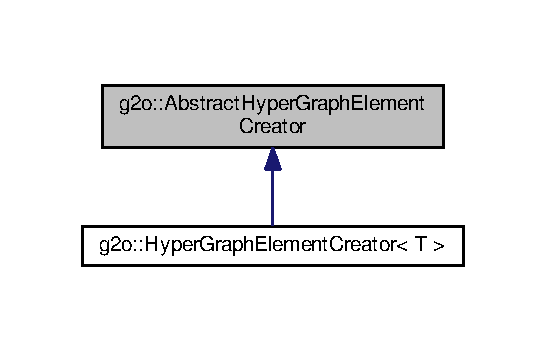
\includegraphics[width=262pt]{classg2o_1_1AbstractHyperGraphElementCreator__inherit__graph}
\end{center}
\end{figure}
\subsection*{Public 成员函数}
\begin{DoxyCompactItemize}
\item 
virtual \\*
\hyperlink{structg2o_1_1HyperGraph_1_1HyperGraphElement}{Hyper\-Graph\-::\-Hyper\-Graph\-Element} $\ast$ \hyperlink{classg2o_1_1AbstractHyperGraphElementCreator_a0b4722fa4b05465bf89d6e7fdc75b153}{construct} ()=0
\item 
virtual const std\-::string \& \hyperlink{classg2o_1_1AbstractHyperGraphElementCreator_a238928fbbfd6e473b2c61002112e6f5f}{name} () const =0
\end{DoxyCompactItemize}


\subsection{详细描述}
Abstract interface for allocating Hyper\-Graph\-Element. 

在文件 creators.\-h 第 43 行定义.



\subsection{成员函数说明}
\hypertarget{classg2o_1_1AbstractHyperGraphElementCreator_a0b4722fa4b05465bf89d6e7fdc75b153}{\index{g2o\-::\-Abstract\-Hyper\-Graph\-Element\-Creator@{g2o\-::\-Abstract\-Hyper\-Graph\-Element\-Creator}!construct@{construct}}
\index{construct@{construct}!g2o::AbstractHyperGraphElementCreator@{g2o\-::\-Abstract\-Hyper\-Graph\-Element\-Creator}}
\subsubsection[{construct}]{\setlength{\rightskip}{0pt plus 5cm}virtual {\bf Hyper\-Graph\-::\-Hyper\-Graph\-Element}$\ast$ g2o\-::\-Abstract\-Hyper\-Graph\-Element\-Creator\-::construct (
\begin{DoxyParamCaption}
{}
\end{DoxyParamCaption}
)\hspace{0.3cm}{\ttfamily [pure virtual]}}}\label{classg2o_1_1AbstractHyperGraphElementCreator_a0b4722fa4b05465bf89d6e7fdc75b153}
create a hyper graph element. Has to implemented in derived class. 

在 \hyperlink{classg2o_1_1HyperGraphElementCreator_af5e58366dd05b49700076e0c4ace31e3}{g2o\-::\-Hyper\-Graph\-Element\-Creator$<$ T $>$} 内被实现.



参考自 g2o\-::\-Factory\-::register\-Type().



这是这个函数的调用关系图\-:
\nopagebreak
\begin{figure}[H]
\begin{center}
\leavevmode
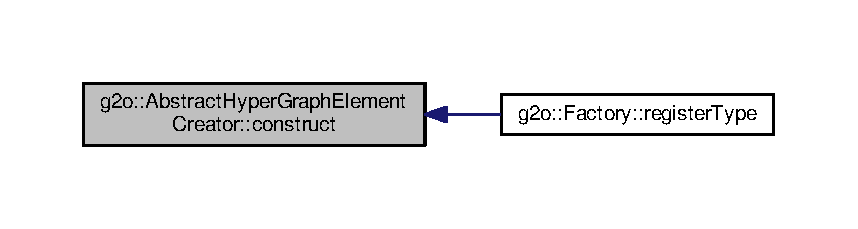
\includegraphics[width=350pt]{classg2o_1_1AbstractHyperGraphElementCreator_a0b4722fa4b05465bf89d6e7fdc75b153_icgraph}
\end{center}
\end{figure}


\hypertarget{classg2o_1_1AbstractHyperGraphElementCreator_a238928fbbfd6e473b2c61002112e6f5f}{\index{g2o\-::\-Abstract\-Hyper\-Graph\-Element\-Creator@{g2o\-::\-Abstract\-Hyper\-Graph\-Element\-Creator}!name@{name}}
\index{name@{name}!g2o::AbstractHyperGraphElementCreator@{g2o\-::\-Abstract\-Hyper\-Graph\-Element\-Creator}}
\subsubsection[{name}]{\setlength{\rightskip}{0pt plus 5cm}virtual const std\-::string\& g2o\-::\-Abstract\-Hyper\-Graph\-Element\-Creator\-::name (
\begin{DoxyParamCaption}
{}
\end{DoxyParamCaption}
) const\hspace{0.3cm}{\ttfamily [pure virtual]}}}\label{classg2o_1_1AbstractHyperGraphElementCreator_a238928fbbfd6e473b2c61002112e6f5f}
name of the class to be created. Has to implemented in derived class. 

在 \hyperlink{classg2o_1_1HyperGraphElementCreator_a48df4ada5c8540e65e6e4925b7a00a04}{g2o\-::\-Hyper\-Graph\-Element\-Creator$<$ T $>$} 内被实现.



参考自 g2o\-::\-Factory\-::register\-Type() , 以及 g2o\-::\-Factory\-::unregister\-Type().



这是这个函数的调用关系图\-:
\nopagebreak
\begin{figure}[H]
\begin{center}
\leavevmode
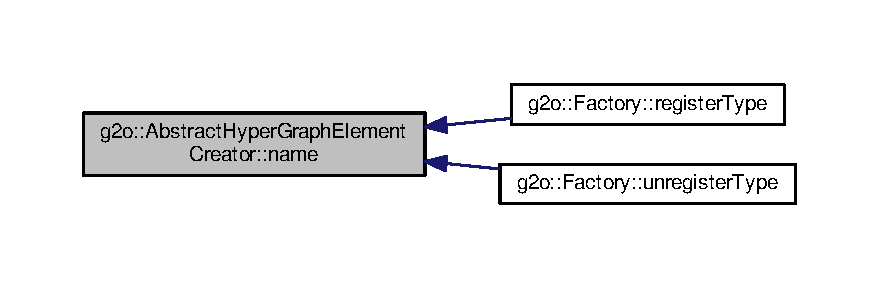
\includegraphics[width=350pt]{classg2o_1_1AbstractHyperGraphElementCreator_a238928fbbfd6e473b2c61002112e6f5f_icgraph}
\end{center}
\end{figure}




该类的文档由以下文件生成\-:\begin{DoxyCompactItemize}
\item 
Thirdparty/g2o/g2o/core/creators.\-h\end{DoxyCompactItemize}

\hypertarget{classg2o_1_1AbstractOptimizationAlgorithmCreator}{\section{g2o\-:\-:Abstract\-Optimization\-Algorithm\-Creator类 参考}
\label{classg2o_1_1AbstractOptimizationAlgorithmCreator}\index{g2o\-::\-Abstract\-Optimization\-Algorithm\-Creator@{g2o\-::\-Abstract\-Optimization\-Algorithm\-Creator}}
}


base for allocating an optimization algorithm  




{\ttfamily \#include $<$optimization\-\_\-algorithm\-\_\-factory.\-h$>$}



g2o\-:\-:Abstract\-Optimization\-Algorithm\-Creator 的协作图\-:
\nopagebreak
\begin{figure}[H]
\begin{center}
\leavevmode
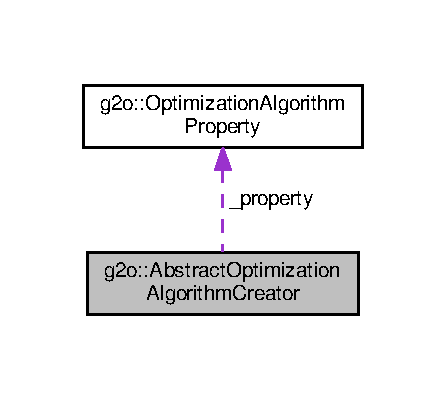
\includegraphics[width=214pt]{classg2o_1_1AbstractOptimizationAlgorithmCreator__coll__graph}
\end{center}
\end{figure}
\subsection*{Public 成员函数}
\begin{DoxyCompactItemize}
\item 
\hypertarget{classg2o_1_1AbstractOptimizationAlgorithmCreator_ae9f64a630d2e641043aabc98660495d8}{{\bfseries Abstract\-Optimization\-Algorithm\-Creator} (const \hyperlink{structg2o_1_1OptimizationAlgorithmProperty}{Optimization\-Algorithm\-Property} \&p)}\label{classg2o_1_1AbstractOptimizationAlgorithmCreator_ae9f64a630d2e641043aabc98660495d8}

\item 
\hypertarget{classg2o_1_1AbstractOptimizationAlgorithmCreator_a96a737bda0f932ac7dd51aa468795353}{virtual \hyperlink{classg2o_1_1OptimizationAlgorithm}{Optimization\-Algorithm} $\ast$ \hyperlink{classg2o_1_1AbstractOptimizationAlgorithmCreator_a96a737bda0f932ac7dd51aa468795353}{construct} ()=0}\label{classg2o_1_1AbstractOptimizationAlgorithmCreator_a96a737bda0f932ac7dd51aa468795353}

\begin{DoxyCompactList}\small\item\em allocate a solver operating on optimizer, re-\/implement for your creator \end{DoxyCompactList}\item 
\hypertarget{classg2o_1_1AbstractOptimizationAlgorithmCreator_af070d079a64f6d23afe6df25e154b160}{const \\*
\hyperlink{structg2o_1_1OptimizationAlgorithmProperty}{Optimization\-Algorithm\-Property} \& \hyperlink{classg2o_1_1AbstractOptimizationAlgorithmCreator_af070d079a64f6d23afe6df25e154b160}{property} () const }\label{classg2o_1_1AbstractOptimizationAlgorithmCreator_af070d079a64f6d23afe6df25e154b160}

\begin{DoxyCompactList}\small\item\em return the properties of the solver \end{DoxyCompactList}\end{DoxyCompactItemize}
\subsection*{Protected 属性}
\begin{DoxyCompactItemize}
\item 
\hypertarget{classg2o_1_1AbstractOptimizationAlgorithmCreator_acf2663d0d6dec71049e4853a9825eafb}{\hyperlink{structg2o_1_1OptimizationAlgorithmProperty}{Optimization\-Algorithm\-Property} {\bfseries \-\_\-property}}\label{classg2o_1_1AbstractOptimizationAlgorithmCreator_acf2663d0d6dec71049e4853a9825eafb}

\end{DoxyCompactItemize}


\subsection{详细描述}
base for allocating an optimization algorithm 

Allocating a solver for a given optimizer. The method \hyperlink{classg2o_1_1AbstractOptimizationAlgorithmCreator_a96a737bda0f932ac7dd51aa468795353}{construct()} has to be implemented in your derived class to allocate the desired solver. 

在文件 optimization\-\_\-algorithm\-\_\-factory.\-h 第 54 行定义.



该类的文档由以下文件生成\-:\begin{DoxyCompactItemize}
\item 
Thirdparty/g2o/g2o/core/optimization\-\_\-algorithm\-\_\-factory.\-h\item 
Thirdparty/g2o/g2o/core/optimization\-\_\-algorithm\-\_\-factory.\-cpp\end{DoxyCompactItemize}

\hypertarget{classg2o_1_1AbstractRobustKernelCreator}{\section{g2o\-:\-:Abstract\-Robust\-Kernel\-Creator类 参考}
\label{classg2o_1_1AbstractRobustKernelCreator}\index{g2o\-::\-Abstract\-Robust\-Kernel\-Creator@{g2o\-::\-Abstract\-Robust\-Kernel\-Creator}}
}


Abstract interface for allocating a robust kernel.  




{\ttfamily \#include $<$robust\-\_\-kernel\-\_\-factory.\-h$>$}



类 g2o\-:\-:Abstract\-Robust\-Kernel\-Creator 继承关系图\-:
\nopagebreak
\begin{figure}[H]
\begin{center}
\leavevmode
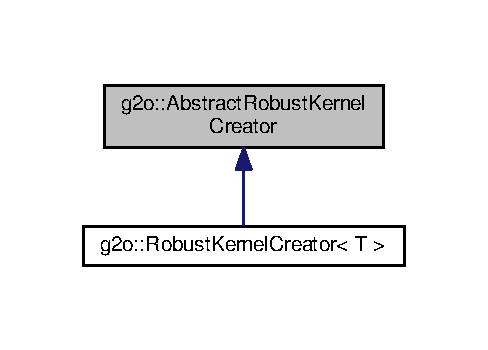
\includegraphics[width=234pt]{classg2o_1_1AbstractRobustKernelCreator__inherit__graph}
\end{center}
\end{figure}
\subsection*{Public 成员函数}
\begin{DoxyCompactItemize}
\item 
virtual \hyperlink{classg2o_1_1RobustKernel}{Robust\-Kernel} $\ast$ \hyperlink{classg2o_1_1AbstractRobustKernelCreator_a3022ab9279e52151d37f8cb4d1524d47}{construct} ()=0
\end{DoxyCompactItemize}


\subsection{详细描述}
Abstract interface for allocating a robust kernel. 

在文件 robust\-\_\-kernel\-\_\-factory.\-h 第 45 行定义.



\subsection{成员函数说明}
\hypertarget{classg2o_1_1AbstractRobustKernelCreator_a3022ab9279e52151d37f8cb4d1524d47}{\index{g2o\-::\-Abstract\-Robust\-Kernel\-Creator@{g2o\-::\-Abstract\-Robust\-Kernel\-Creator}!construct@{construct}}
\index{construct@{construct}!g2o::AbstractRobustKernelCreator@{g2o\-::\-Abstract\-Robust\-Kernel\-Creator}}
\subsubsection[{construct}]{\setlength{\rightskip}{0pt plus 5cm}virtual {\bf Robust\-Kernel}$\ast$ g2o\-::\-Abstract\-Robust\-Kernel\-Creator\-::construct (
\begin{DoxyParamCaption}
{}
\end{DoxyParamCaption}
)\hspace{0.3cm}{\ttfamily [pure virtual]}}}\label{classg2o_1_1AbstractRobustKernelCreator_a3022ab9279e52151d37f8cb4d1524d47}
create a hyper graph element. Has to implemented in derived class. 

在 \hyperlink{classg2o_1_1RobustKernelCreator_a6ab30adc017675641bd55502d7da0085}{g2o\-::\-Robust\-Kernel\-Creator$<$ T $>$} 内被实现.



该类的文档由以下文件生成\-:\begin{DoxyCompactItemize}
\item 
Thirdparty/g2o/g2o/core/robust\-\_\-kernel\-\_\-factory.\-h\end{DoxyCompactItemize}

\hypertarget{classg2o_1_1EstimatePropagator_1_1AdjacencyMapEntry}{\section{g2o\-:\-:Estimate\-Propagator\-:\-:Adjacency\-Map\-Entry类 参考}
\label{classg2o_1_1EstimatePropagator_1_1AdjacencyMapEntry}\index{g2o\-::\-Estimate\-Propagator\-::\-Adjacency\-Map\-Entry@{g2o\-::\-Estimate\-Propagator\-::\-Adjacency\-Map\-Entry}}
}


data structure for loopuk during Dijkstra  




{\ttfamily \#include $<$estimate\-\_\-propagator.\-h$>$}



g2o\-:\-:Estimate\-Propagator\-:\-:Adjacency\-Map\-Entry 的协作图\-:
\nopagebreak
\begin{figure}[H]
\begin{center}
\leavevmode
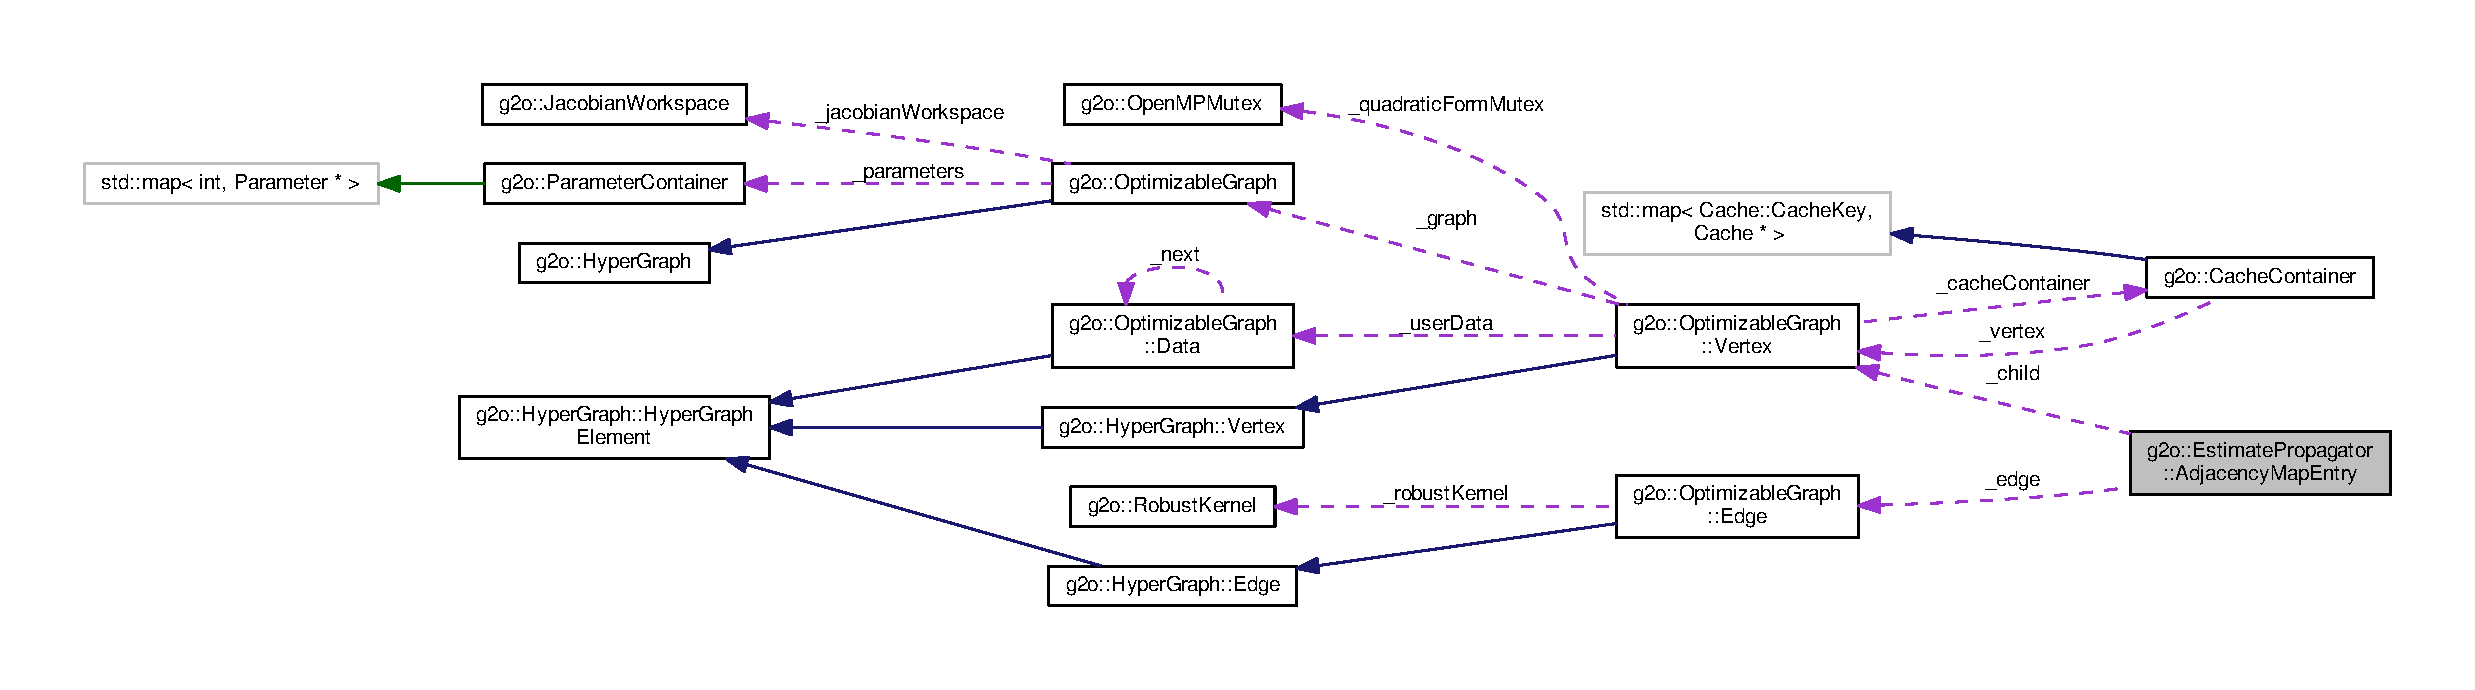
\includegraphics[width=350pt]{classg2o_1_1EstimatePropagator_1_1AdjacencyMapEntry__coll__graph}
\end{center}
\end{figure}
\subsection*{Public 成员函数}
\begin{DoxyCompactItemize}
\item 
\hypertarget{classg2o_1_1EstimatePropagator_1_1AdjacencyMapEntry_a6d2f95439aa6ee608f2e2d110de553e8}{void {\bfseries reset} ()}\label{classg2o_1_1EstimatePropagator_1_1AdjacencyMapEntry_a6d2f95439aa6ee608f2e2d110de553e8}

\item 
\hypertarget{classg2o_1_1EstimatePropagator_1_1AdjacencyMapEntry_a18950202077ae522b96798e7413f87d8}{\hyperlink{classg2o_1_1OptimizableGraph_1_1Vertex}{Optimizable\-Graph\-::\-Vertex} $\ast$ {\bfseries child} () const }\label{classg2o_1_1EstimatePropagator_1_1AdjacencyMapEntry_a18950202077ae522b96798e7413f87d8}

\item 
\hypertarget{classg2o_1_1EstimatePropagator_1_1AdjacencyMapEntry_aee0f4d6633710a78e9db0da72fbc4160}{const Optimizable\-Graph\-::\-Vertex\-Set \& {\bfseries parent} () const }\label{classg2o_1_1EstimatePropagator_1_1AdjacencyMapEntry_aee0f4d6633710a78e9db0da72fbc4160}

\item 
\hypertarget{classg2o_1_1EstimatePropagator_1_1AdjacencyMapEntry_a60bf7d0054f60b3b97cb6ddbb4e6822e}{\hyperlink{classg2o_1_1OptimizableGraph_1_1Edge}{Optimizable\-Graph\-::\-Edge} $\ast$ {\bfseries edge} () const }\label{classg2o_1_1EstimatePropagator_1_1AdjacencyMapEntry_a60bf7d0054f60b3b97cb6ddbb4e6822e}

\item 
\hypertarget{classg2o_1_1EstimatePropagator_1_1AdjacencyMapEntry_a6d09d8c8149ccebebda9bb4f93da475d}{double {\bfseries distance} () const }\label{classg2o_1_1EstimatePropagator_1_1AdjacencyMapEntry_a6d09d8c8149ccebebda9bb4f93da475d}

\item 
\hypertarget{classg2o_1_1EstimatePropagator_1_1AdjacencyMapEntry_aa198f0e42ac773dc34a42ab9b75d3a08}{int {\bfseries frontier\-Level} () const }\label{classg2o_1_1EstimatePropagator_1_1AdjacencyMapEntry_aa198f0e42ac773dc34a42ab9b75d3a08}

\end{DoxyCompactItemize}
\subsection*{Protected 属性}
\begin{DoxyCompactItemize}
\item 
\hypertarget{classg2o_1_1EstimatePropagator_1_1AdjacencyMapEntry_ab6f716e85cc15e6d9c570132fe889fd6}{\hyperlink{classg2o_1_1OptimizableGraph_1_1Vertex}{Optimizable\-Graph\-::\-Vertex} $\ast$ {\bfseries \-\_\-child}}\label{classg2o_1_1EstimatePropagator_1_1AdjacencyMapEntry_ab6f716e85cc15e6d9c570132fe889fd6}

\item 
\hypertarget{classg2o_1_1EstimatePropagator_1_1AdjacencyMapEntry_a72384502361d60e1f3ae1644de1e7379}{Optimizable\-Graph\-::\-Vertex\-Set {\bfseries \-\_\-parent}}\label{classg2o_1_1EstimatePropagator_1_1AdjacencyMapEntry_a72384502361d60e1f3ae1644de1e7379}

\item 
\hypertarget{classg2o_1_1EstimatePropagator_1_1AdjacencyMapEntry_a738795d0b3989374ba51821354629d64}{\hyperlink{classg2o_1_1OptimizableGraph_1_1Edge}{Optimizable\-Graph\-::\-Edge} $\ast$ {\bfseries \-\_\-edge}}\label{classg2o_1_1EstimatePropagator_1_1AdjacencyMapEntry_a738795d0b3989374ba51821354629d64}

\item 
\hypertarget{classg2o_1_1EstimatePropagator_1_1AdjacencyMapEntry_a3558503af9d9f56088ff1593398f86d4}{double {\bfseries \-\_\-distance}}\label{classg2o_1_1EstimatePropagator_1_1AdjacencyMapEntry_a3558503af9d9f56088ff1593398f86d4}

\item 
\hypertarget{classg2o_1_1EstimatePropagator_1_1AdjacencyMapEntry_a56bfab4074fa692f03378526007758f7}{int {\bfseries \-\_\-frontier\-Level}}\label{classg2o_1_1EstimatePropagator_1_1AdjacencyMapEntry_a56bfab4074fa692f03378526007758f7}

\end{DoxyCompactItemize}
\subsection*{友元}
\begin{DoxyCompactItemize}
\item 
\hypertarget{classg2o_1_1EstimatePropagator_1_1AdjacencyMapEntry_a84fd16bbb058a331370b1b9983896264}{class {\bfseries Estimate\-Propagator}}\label{classg2o_1_1EstimatePropagator_1_1AdjacencyMapEntry_a84fd16bbb058a331370b1b9983896264}

\item 
\hypertarget{classg2o_1_1EstimatePropagator_1_1AdjacencyMapEntry_afde21c6f1b41de5a73362b2fcfec056b}{class {\bfseries Priority\-Queue}}\label{classg2o_1_1EstimatePropagator_1_1AdjacencyMapEntry_afde21c6f1b41de5a73362b2fcfec056b}

\end{DoxyCompactItemize}


\subsection{详细描述}
data structure for loopuk during Dijkstra 

在文件 estimate\-\_\-propagator.\-h 第 110 行定义.



该类的文档由以下文件生成\-:\begin{DoxyCompactItemize}
\item 
Thirdparty/g2o/g2o/core/estimate\-\_\-propagator.\-h\item 
Thirdparty/g2o/g2o/core/estimate\-\_\-propagator.\-cpp\end{DoxyCompactItemize}

\hypertarget{structg2o_1_1HyperDijkstra_1_1AdjacencyMapEntry}{\section{g2o\-:\-:Hyper\-Dijkstra\-:\-:Adjacency\-Map\-Entry结构体 参考}
\label{structg2o_1_1HyperDijkstra_1_1AdjacencyMapEntry}\index{g2o\-::\-Hyper\-Dijkstra\-::\-Adjacency\-Map\-Entry@{g2o\-::\-Hyper\-Dijkstra\-::\-Adjacency\-Map\-Entry}}
}


g2o\-:\-:Hyper\-Dijkstra\-:\-:Adjacency\-Map\-Entry 的协作图\-:
\nopagebreak
\begin{figure}[H]
\begin{center}
\leavevmode
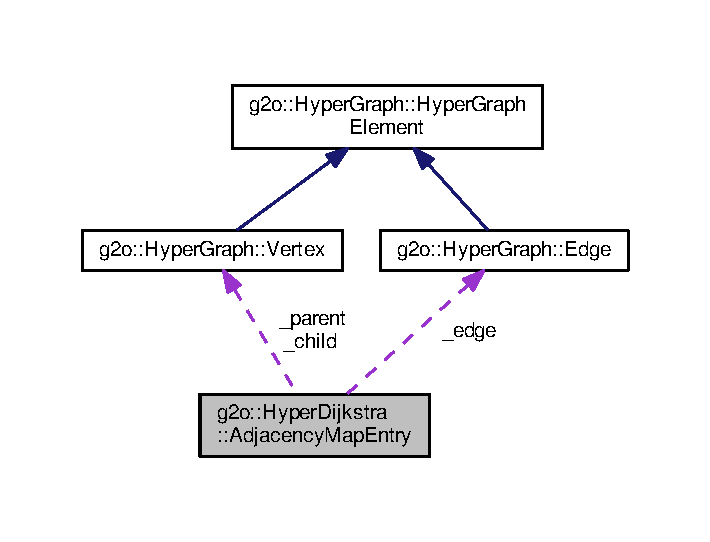
\includegraphics[width=341pt]{structg2o_1_1HyperDijkstra_1_1AdjacencyMapEntry__coll__graph}
\end{center}
\end{figure}
\subsection*{Public 成员函数}
\begin{DoxyCompactItemize}
\item 
\hypertarget{structg2o_1_1HyperDijkstra_1_1AdjacencyMapEntry_a160f87d80b7c2137abcce561fbc5feed}{{\bfseries Adjacency\-Map\-Entry} (\hyperlink{classg2o_1_1HyperGraph_1_1Vertex}{Hyper\-Graph\-::\-Vertex} $\ast$\-\_\-child=0, \hyperlink{classg2o_1_1HyperGraph_1_1Vertex}{Hyper\-Graph\-::\-Vertex} $\ast$\-\_\-parent=0, \hyperlink{classg2o_1_1HyperGraph_1_1Edge}{Hyper\-Graph\-::\-Edge} $\ast$\-\_\-edge=0, double \-\_\-distance=std\-::numeric\-\_\-limits$<$ double $>$\-::max())}\label{structg2o_1_1HyperDijkstra_1_1AdjacencyMapEntry_a160f87d80b7c2137abcce561fbc5feed}

\item 
\hypertarget{structg2o_1_1HyperDijkstra_1_1AdjacencyMapEntry_a16b56779c464b948cb0a102929e1c5f2}{\hyperlink{classg2o_1_1HyperGraph_1_1Vertex}{Hyper\-Graph\-::\-Vertex} $\ast$ {\bfseries child} () const }\label{structg2o_1_1HyperDijkstra_1_1AdjacencyMapEntry_a16b56779c464b948cb0a102929e1c5f2}

\item 
\hypertarget{structg2o_1_1HyperDijkstra_1_1AdjacencyMapEntry_a2955ede218d2843f1ceae9402e3a9c23}{\hyperlink{classg2o_1_1HyperGraph_1_1Vertex}{Hyper\-Graph\-::\-Vertex} $\ast$ {\bfseries parent} () const }\label{structg2o_1_1HyperDijkstra_1_1AdjacencyMapEntry_a2955ede218d2843f1ceae9402e3a9c23}

\item 
\hypertarget{structg2o_1_1HyperDijkstra_1_1AdjacencyMapEntry_a4cbdf1ab4ad29ab534cad318ca6898dc}{\hyperlink{classg2o_1_1HyperGraph_1_1Edge}{Hyper\-Graph\-::\-Edge} $\ast$ {\bfseries edge} () const }\label{structg2o_1_1HyperDijkstra_1_1AdjacencyMapEntry_a4cbdf1ab4ad29ab534cad318ca6898dc}

\item 
\hypertarget{structg2o_1_1HyperDijkstra_1_1AdjacencyMapEntry_a40a498bd2fae5c3a4a25d91599e22f9f}{double {\bfseries distance} () const }\label{structg2o_1_1HyperDijkstra_1_1AdjacencyMapEntry_a40a498bd2fae5c3a4a25d91599e22f9f}

\item 
\hypertarget{structg2o_1_1HyperDijkstra_1_1AdjacencyMapEntry_aa1a11048612968381db6a0ad525f7e0d}{Hyper\-Graph\-::\-Vertex\-Set \& {\bfseries children} ()}\label{structg2o_1_1HyperDijkstra_1_1AdjacencyMapEntry_aa1a11048612968381db6a0ad525f7e0d}

\item 
\hypertarget{structg2o_1_1HyperDijkstra_1_1AdjacencyMapEntry_a631ac78faf06416839df66a8c93aab9e}{const Hyper\-Graph\-::\-Vertex\-Set \& {\bfseries children} () const }\label{structg2o_1_1HyperDijkstra_1_1AdjacencyMapEntry_a631ac78faf06416839df66a8c93aab9e}

\end{DoxyCompactItemize}
\subsection*{Protected 属性}
\begin{DoxyCompactItemize}
\item 
\hypertarget{structg2o_1_1HyperDijkstra_1_1AdjacencyMapEntry_a7ccdf917414efa537c3942d360ca127a}{\hyperlink{classg2o_1_1HyperGraph_1_1Vertex}{Hyper\-Graph\-::\-Vertex} $\ast$ {\bfseries \-\_\-child}}\label{structg2o_1_1HyperDijkstra_1_1AdjacencyMapEntry_a7ccdf917414efa537c3942d360ca127a}

\item 
\hypertarget{structg2o_1_1HyperDijkstra_1_1AdjacencyMapEntry_a3490ab9668c98d3e0cb14c54b9d41747}{\hyperlink{classg2o_1_1HyperGraph_1_1Vertex}{Hyper\-Graph\-::\-Vertex} $\ast$ {\bfseries \-\_\-parent}}\label{structg2o_1_1HyperDijkstra_1_1AdjacencyMapEntry_a3490ab9668c98d3e0cb14c54b9d41747}

\item 
\hypertarget{structg2o_1_1HyperDijkstra_1_1AdjacencyMapEntry_adc56c13a328aac02456474a9e7c72415}{\hyperlink{classg2o_1_1HyperGraph_1_1Edge}{Hyper\-Graph\-::\-Edge} $\ast$ {\bfseries \-\_\-edge}}\label{structg2o_1_1HyperDijkstra_1_1AdjacencyMapEntry_adc56c13a328aac02456474a9e7c72415}

\item 
\hypertarget{structg2o_1_1HyperDijkstra_1_1AdjacencyMapEntry_a95b3db28f32badcdce2edf1bae83b78d}{double {\bfseries \-\_\-distance}}\label{structg2o_1_1HyperDijkstra_1_1AdjacencyMapEntry_a95b3db28f32badcdce2edf1bae83b78d}

\item 
\hypertarget{structg2o_1_1HyperDijkstra_1_1AdjacencyMapEntry_a5b69ff3769d50a3229e2df80cac3f093}{Hyper\-Graph\-::\-Vertex\-Set {\bfseries \-\_\-children}}\label{structg2o_1_1HyperDijkstra_1_1AdjacencyMapEntry_a5b69ff3769d50a3229e2df80cac3f093}

\end{DoxyCompactItemize}
\subsection*{友元}
\begin{DoxyCompactItemize}
\item 
\hypertarget{structg2o_1_1HyperDijkstra_1_1AdjacencyMapEntry_a358d802df25b35f34e715710d1fa380c}{struct {\bfseries Hyper\-Dijkstra}}\label{structg2o_1_1HyperDijkstra_1_1AdjacencyMapEntry_a358d802df25b35f34e715710d1fa380c}

\end{DoxyCompactItemize}


\subsection{详细描述}


在文件 hyper\-\_\-dijkstra.\-h 第 51 行定义.



该结构体的文档由以下文件生成\-:\begin{DoxyCompactItemize}
\item 
Thirdparty/g2o/g2o/core/hyper\-\_\-dijkstra.\-h\item 
Thirdparty/g2o/g2o/core/hyper\-\_\-dijkstra.\-cpp\end{DoxyCompactItemize}

\hypertarget{classg2o_1_1BaseBinaryEdge}{\section{g2o\-:\-:Base\-Binary\-Edge$<$ D, E, Vertex\-Xi, Vertex\-Xj $>$ 模板类 参考}
\label{classg2o_1_1BaseBinaryEdge}\index{g2o\-::\-Base\-Binary\-Edge$<$ D, E, Vertex\-Xi, Vertex\-Xj $>$@{g2o\-::\-Base\-Binary\-Edge$<$ D, E, Vertex\-Xi, Vertex\-Xj $>$}}
}


类 g2o\-:\-:Base\-Binary\-Edge$<$ D, E, Vertex\-Xi, Vertex\-Xj $>$ 继承关系图\-:
\nopagebreak
\begin{figure}[H]
\begin{center}
\leavevmode
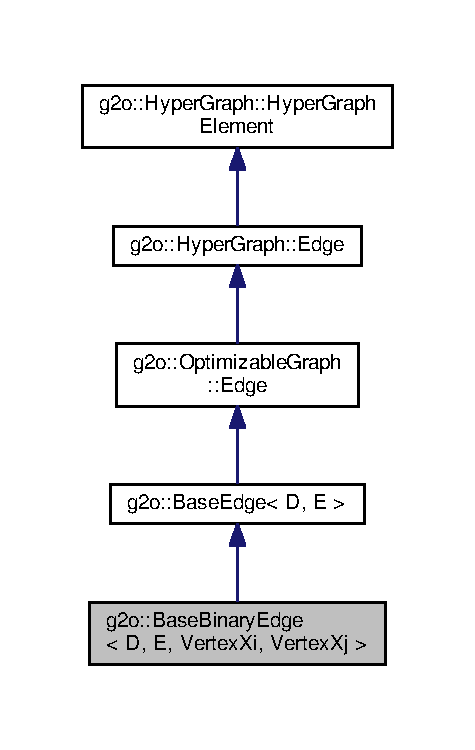
\includegraphics[width=228pt]{classg2o_1_1BaseBinaryEdge__inherit__graph}
\end{center}
\end{figure}


g2o\-:\-:Base\-Binary\-Edge$<$ D, E, Vertex\-Xi, Vertex\-Xj $>$ 的协作图\-:
\nopagebreak
\begin{figure}[H]
\begin{center}
\leavevmode
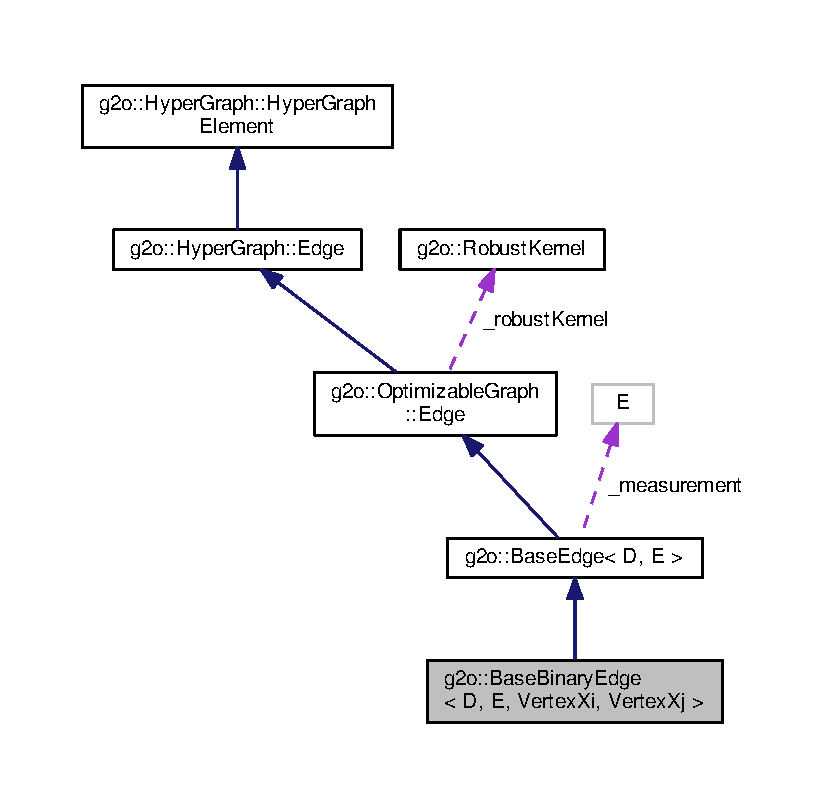
\includegraphics[width=350pt]{classg2o_1_1BaseBinaryEdge__coll__graph}
\end{center}
\end{figure}
\subsection*{Public 类型}
\begin{DoxyCompactItemize}
\item 
\hypertarget{classg2o_1_1BaseBinaryEdge_aa8e2b04b2c0c90adc48384d6d41063cc}{typedef Vertex\-Xi {\bfseries Vertex\-Xi\-Type}}\label{classg2o_1_1BaseBinaryEdge_aa8e2b04b2c0c90adc48384d6d41063cc}

\item 
\hypertarget{classg2o_1_1BaseBinaryEdge_aa489ae37680c37d7b2c3c1a197f90de9}{typedef Vertex\-Xj {\bfseries Vertex\-Xj\-Type}}\label{classg2o_1_1BaseBinaryEdge_aa489ae37680c37d7b2c3c1a197f90de9}

\item 
\hypertarget{classg2o_1_1BaseBinaryEdge_ac1e9249e9906747a6669a9c90013944b}{typedef \hyperlink{classg2o_1_1BaseEdge}{Base\-Edge}$<$ D, E $>$\\*
\-::Measurement {\bfseries Measurement}}\label{classg2o_1_1BaseBinaryEdge_ac1e9249e9906747a6669a9c90013944b}

\item 
\hypertarget{classg2o_1_1BaseBinaryEdge_ab1cde84224b129603bcd95db027e0167}{typedef Matrix$<$ double, D, Di $>$\\*
\-::Aligned\-Map\-Type {\bfseries Jacobian\-Xi\-Oplus\-Type}}\label{classg2o_1_1BaseBinaryEdge_ab1cde84224b129603bcd95db027e0167}

\item 
\hypertarget{classg2o_1_1BaseBinaryEdge_a83e5dec2135b33e86255c87be3b5d062}{typedef Matrix$<$ double, D, Dj $>$\\*
\-::Aligned\-Map\-Type {\bfseries Jacobian\-Xj\-Oplus\-Type}}\label{classg2o_1_1BaseBinaryEdge_a83e5dec2135b33e86255c87be3b5d062}

\item 
\hypertarget{classg2o_1_1BaseBinaryEdge_ae1cccf6068b2446ece316b6a69a46acf}{typedef \hyperlink{classg2o_1_1BaseEdge}{Base\-Edge}$<$ D, E $>$\\*
\-::Error\-Vector {\bfseries Error\-Vector}}\label{classg2o_1_1BaseBinaryEdge_ae1cccf6068b2446ece316b6a69a46acf}

\item 
\hypertarget{classg2o_1_1BaseBinaryEdge_a4530ef6462aadaf2ab826d440d3b3318}{typedef \hyperlink{classg2o_1_1BaseEdge}{Base\-Edge}$<$ D, E $>$\\*
\-::Information\-Type {\bfseries Information\-Type}}\label{classg2o_1_1BaseBinaryEdge_a4530ef6462aadaf2ab826d440d3b3318}

\item 
\hypertarget{classg2o_1_1BaseBinaryEdge_a7eadbbe6abffe4d2ebdf6231272789a5}{typedef Eigen\-::\-Map$<$ Matrix\\*
$<$ double, Di, Dj $>$, Matrix\\*
$<$ double, Di, Dj $>$\-::Flags \\*
\&Aligned\-Bit?Aligned\-:\-Unaligned $>$ {\bfseries Hessian\-Block\-Type}}\label{classg2o_1_1BaseBinaryEdge_a7eadbbe6abffe4d2ebdf6231272789a5}

\item 
\hypertarget{classg2o_1_1BaseBinaryEdge_aec0d5b1819f702b7658574fcd6324b49}{typedef Eigen\-::\-Map$<$ Matrix\\*
$<$ double, Dj, Di $>$, Matrix\\*
$<$ double, Dj, Di $>$\-::Flags \\*
\&Aligned\-Bit?Aligned\-:\-Unaligned $>$ {\bfseries Hessian\-Block\-Transposed\-Type}}\label{classg2o_1_1BaseBinaryEdge_aec0d5b1819f702b7658574fcd6324b49}

\end{DoxyCompactItemize}
\subsection*{Public 成员函数}
\begin{DoxyCompactItemize}
\item 
\hypertarget{classg2o_1_1BaseBinaryEdge_a32bfc93b6dede619c7d99db2fb60f80d}{virtual \hyperlink{classg2o_1_1OptimizableGraph_1_1Vertex}{Optimizable\-Graph\-::\-Vertex} $\ast$ {\bfseries create\-From} ()}\label{classg2o_1_1BaseBinaryEdge_a32bfc93b6dede619c7d99db2fb60f80d}

\item 
\hypertarget{classg2o_1_1BaseBinaryEdge_ac7cce17e3229445e5a33c3cb8a569320}{virtual \hyperlink{classg2o_1_1OptimizableGraph_1_1Vertex}{Optimizable\-Graph\-::\-Vertex} $\ast$ {\bfseries create\-To} ()}\label{classg2o_1_1BaseBinaryEdge_ac7cce17e3229445e5a33c3cb8a569320}

\item 
virtual void \hyperlink{classg2o_1_1BaseBinaryEdge_a06e64067fa5fff4a5e2d058249b55478}{resize} (size\-\_\-t size)
\item 
\hypertarget{classg2o_1_1BaseBinaryEdge_a1895c3b7141e93fd05bf271daeda7568}{virtual bool {\bfseries all\-Vertices\-Fixed} () const }\label{classg2o_1_1BaseBinaryEdge_a1895c3b7141e93fd05bf271daeda7568}

\item 
virtual void \hyperlink{classg2o_1_1BaseBinaryEdge_afc3b6470e7679f027c2614484b394925}{linearize\-Oplus} (\hyperlink{classg2o_1_1JacobianWorkspace}{Jacobian\-Workspace} \&jacobian\-Workspace)
\item 
virtual void \hyperlink{classg2o_1_1BaseBinaryEdge_af0fb8a693c8c7996fa65566e7263fbc4}{linearize\-Oplus} ()
\item 
\hypertarget{classg2o_1_1BaseBinaryEdge_ad036a59a5bc1d04d1799d61b9be15864}{const Jacobian\-Xi\-Oplus\-Type \& \hyperlink{classg2o_1_1BaseBinaryEdge_ad036a59a5bc1d04d1799d61b9be15864}{jacobian\-Oplus\-Xi} () const }\label{classg2o_1_1BaseBinaryEdge_ad036a59a5bc1d04d1799d61b9be15864}

\begin{DoxyCompactList}\small\item\em returns the result of the linearization in the manifold space for the node xi \end{DoxyCompactList}\item 
\hypertarget{classg2o_1_1BaseBinaryEdge_a8a8ed568c4a00f74943fc1efe5bbc72c}{const Jacobian\-Xj\-Oplus\-Type \& \hyperlink{classg2o_1_1BaseBinaryEdge_a8a8ed568c4a00f74943fc1efe5bbc72c}{jacobian\-Oplus\-Xj} () const }\label{classg2o_1_1BaseBinaryEdge_a8a8ed568c4a00f74943fc1efe5bbc72c}

\begin{DoxyCompactList}\small\item\em returns the result of the linearization in the manifold space for the node xj \end{DoxyCompactList}\item 
virtual void \hyperlink{classg2o_1_1BaseBinaryEdge_a06a18745d95017c6d3c841f838a65364}{construct\-Quadratic\-Form} ()
\item 
virtual void \hyperlink{classg2o_1_1BaseBinaryEdge_ada358930854d386a4e8c32f64078e052}{map\-Hessian\-Memory} (double $\ast$d, int i, int j, bool row\-Major)
\end{DoxyCompactItemize}
\subsection*{静态 Public 属性}
\begin{DoxyCompactItemize}
\item 
\hypertarget{classg2o_1_1BaseBinaryEdge_abfe232196405a7204bc299a747c1cc8b}{static const int {\bfseries Di} = Vertex\-Xi\-Type\-::\-Dimension}\label{classg2o_1_1BaseBinaryEdge_abfe232196405a7204bc299a747c1cc8b}

\item 
\hypertarget{classg2o_1_1BaseBinaryEdge_ab718b94950a34d589371fe6f5583b259}{static const int {\bfseries Dj} = Vertex\-Xj\-Type\-::\-Dimension}\label{classg2o_1_1BaseBinaryEdge_ab718b94950a34d589371fe6f5583b259}

\item 
\hypertarget{classg2o_1_1BaseBinaryEdge_af3c134948e48c446762fa4e427d1cca5}{static const int {\bfseries Dimension} = \hyperlink{classg2o_1_1BaseEdge}{Base\-Edge}$<$D, E$>$\-::Dimension}\label{classg2o_1_1BaseBinaryEdge_af3c134948e48c446762fa4e427d1cca5}

\end{DoxyCompactItemize}
\subsection*{Protected 属性}
\begin{DoxyCompactItemize}
\item 
\hypertarget{classg2o_1_1BaseBinaryEdge_aeb5c1f09a4433a6bd76ce4ab67bd9a64}{bool {\bfseries \-\_\-hessian\-Row\-Major}}\label{classg2o_1_1BaseBinaryEdge_aeb5c1f09a4433a6bd76ce4ab67bd9a64}

\item 
\hypertarget{classg2o_1_1BaseBinaryEdge_a5036f75e3b20c79cb014fcc929d8eef9}{Hessian\-Block\-Type {\bfseries \-\_\-hessian}}\label{classg2o_1_1BaseBinaryEdge_a5036f75e3b20c79cb014fcc929d8eef9}

\item 
\hypertarget{classg2o_1_1BaseBinaryEdge_aa61657904b00fcfa19df382094386f11}{Hessian\-Block\-Transposed\-Type {\bfseries \-\_\-hessian\-Transposed}}\label{classg2o_1_1BaseBinaryEdge_aa61657904b00fcfa19df382094386f11}

\item 
\hypertarget{classg2o_1_1BaseBinaryEdge_aa21b9d84924ec93192374761ee0adfa7}{Jacobian\-Xi\-Oplus\-Type {\bfseries \-\_\-jacobian\-Oplus\-Xi}}\label{classg2o_1_1BaseBinaryEdge_aa21b9d84924ec93192374761ee0adfa7}

\item 
\hypertarget{classg2o_1_1BaseBinaryEdge_ad448518247044496cb99c9d70bd1a363}{Jacobian\-Xj\-Oplus\-Type {\bfseries \-\_\-jacobian\-Oplus\-Xj}}\label{classg2o_1_1BaseBinaryEdge_ad448518247044496cb99c9d70bd1a363}

\end{DoxyCompactItemize}
\subsection*{额外继承的成员函数}


\subsection{详细描述}
\subsubsection*{template$<$int D, typename E, typename Vertex\-Xi, typename Vertex\-Xj$>$class g2o\-::\-Base\-Binary\-Edge$<$ D, E, Vertex\-Xi, Vertex\-Xj $>$}



在文件 base\-\_\-binary\-\_\-edge.\-h 第 42 行定义.



\subsection{成员函数说明}
\hypertarget{classg2o_1_1BaseBinaryEdge_a06a18745d95017c6d3c841f838a65364}{\index{g2o\-::\-Base\-Binary\-Edge@{g2o\-::\-Base\-Binary\-Edge}!construct\-Quadratic\-Form@{construct\-Quadratic\-Form}}
\index{construct\-Quadratic\-Form@{construct\-Quadratic\-Form}!g2o::BaseBinaryEdge@{g2o\-::\-Base\-Binary\-Edge}}
\subsubsection[{construct\-Quadratic\-Form}]{\setlength{\rightskip}{0pt plus 5cm}template$<$int D, typename E , typename Vertex\-Xi\-Type , typename Vertex\-Xj\-Type $>$ void Base\-Binary\-Edge\-::construct\-Quadratic\-Form (
\begin{DoxyParamCaption}
{}
\end{DoxyParamCaption}
)\hspace{0.3cm}{\ttfamily [virtual]}}}\label{classg2o_1_1BaseBinaryEdge_a06a18745d95017c6d3c841f838a65364}
Linearizes the constraint in the edge. Makes side effect on the vertices of the graph by changing the parameter vector b and the hessian blocks ii and jj. The off diagoinal block is accesed via \-\_\-hessian. 

实现了 \hyperlink{classg2o_1_1OptimizableGraph_1_1Edge_a56fbf3430ddf591e3c619bdd1b7e4499}{g2o\-::\-Optimizable\-Graph\-::\-Edge}.



在文件 base\-\_\-binary\-\_\-edge.\-h 第 56 行定义.



参考 g2o\-::\-Hyper\-Graph\-::\-Edge\-::resize().



函数调用图\-:
\nopagebreak
\begin{figure}[H]
\begin{center}
\leavevmode
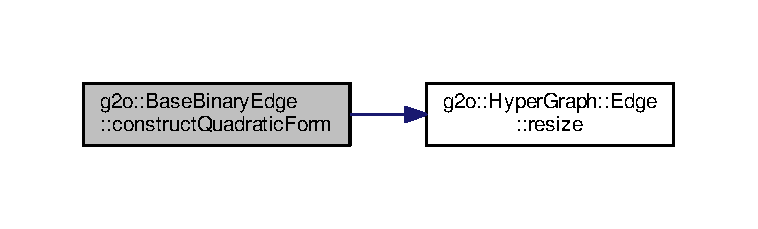
\includegraphics[width=350pt]{classg2o_1_1BaseBinaryEdge_a06a18745d95017c6d3c841f838a65364_cgraph}
\end{center}
\end{figure}


\hypertarget{classg2o_1_1BaseBinaryEdge_afc3b6470e7679f027c2614484b394925}{\index{g2o\-::\-Base\-Binary\-Edge@{g2o\-::\-Base\-Binary\-Edge}!linearize\-Oplus@{linearize\-Oplus}}
\index{linearize\-Oplus@{linearize\-Oplus}!g2o::BaseBinaryEdge@{g2o\-::\-Base\-Binary\-Edge}}
\subsubsection[{linearize\-Oplus}]{\setlength{\rightskip}{0pt plus 5cm}template$<$int D, typename E , typename Vertex\-Xi\-Type , typename Vertex\-Xj\-Type $>$ void Base\-Binary\-Edge\-::linearize\-Oplus (
\begin{DoxyParamCaption}
\item[{{\bf Jacobian\-Workspace} \&}]{jacobian\-Workspace}
\end{DoxyParamCaption}
)\hspace{0.3cm}{\ttfamily [virtual]}}}\label{classg2o_1_1BaseBinaryEdge_afc3b6470e7679f027c2614484b394925}
Linearizes the constraint in the edge in the manifold space, and store the result in the given workspace 

实现了 \hyperlink{classg2o_1_1OptimizableGraph_1_1Edge_a0fdad5ebfb4efec9f893b57f67e0fbe1}{g2o\-::\-Optimizable\-Graph\-::\-Edge}.



在文件 base\-\_\-binary\-\_\-edge.\-h 第 124 行定义.

\hypertarget{classg2o_1_1BaseBinaryEdge_af0fb8a693c8c7996fa65566e7263fbc4}{\index{g2o\-::\-Base\-Binary\-Edge@{g2o\-::\-Base\-Binary\-Edge}!linearize\-Oplus@{linearize\-Oplus}}
\index{linearize\-Oplus@{linearize\-Oplus}!g2o::BaseBinaryEdge@{g2o\-::\-Base\-Binary\-Edge}}
\subsubsection[{linearize\-Oplus}]{\setlength{\rightskip}{0pt plus 5cm}template$<$int D, typename E , typename Vertex\-Xi\-Type , typename Vertex\-Xj\-Type $>$ void Base\-Binary\-Edge\-::linearize\-Oplus (
\begin{DoxyParamCaption}
{}
\end{DoxyParamCaption}
)\hspace{0.3cm}{\ttfamily [virtual]}}}\label{classg2o_1_1BaseBinaryEdge_af0fb8a693c8c7996fa65566e7263fbc4}
Linearizes the oplus operator in the vertex, and stores the result in temporary variables \-\_\-jacobian\-Oplus\-Xi and \-\_\-jacobian\-Oplus\-Xj 

被 \hyperlink{classg2o_1_1EdgeStereoSE3ProjectXYZ_aea04d86a304c6cb4e2a3f34b35166f30}{g2o\-::\-Edge\-Stereo\-S\-E3\-Project\-X\-Y\-Z} , 以及 \hyperlink{classg2o_1_1EdgeSE3ProjectXYZ_a7454e89740635d782c9e4efaef35ec44}{g2o\-::\-Edge\-S\-E3\-Project\-X\-Y\-Z} 重载.



在文件 base\-\_\-binary\-\_\-edge.\-h 第 132 行定义.

\hypertarget{classg2o_1_1BaseBinaryEdge_ada358930854d386a4e8c32f64078e052}{\index{g2o\-::\-Base\-Binary\-Edge@{g2o\-::\-Base\-Binary\-Edge}!map\-Hessian\-Memory@{map\-Hessian\-Memory}}
\index{map\-Hessian\-Memory@{map\-Hessian\-Memory}!g2o::BaseBinaryEdge@{g2o\-::\-Base\-Binary\-Edge}}
\subsubsection[{map\-Hessian\-Memory}]{\setlength{\rightskip}{0pt plus 5cm}template$<$int D, typename E , typename Vertex\-Xi\-Type , typename Vertex\-Xj\-Type $>$ void Base\-Binary\-Edge\-::map\-Hessian\-Memory (
\begin{DoxyParamCaption}
\item[{double $\ast$}]{d, }
\item[{int}]{i, }
\item[{int}]{j, }
\item[{bool}]{row\-Major}
\end{DoxyParamCaption}
)\hspace{0.3cm}{\ttfamily [virtual]}}}\label{classg2o_1_1BaseBinaryEdge_ada358930854d386a4e8c32f64078e052}
maps the internal matrix to some external memory location, you need to provide the memory before calling construct\-Quadratic\-Form 
\begin{DoxyParams}{参数}
{\em d} & the memory location to which we map \\
\hline
{\em i} & index of the vertex i \\
\hline
{\em j} & index of the vertex j (j $>$ i, upper triangular fashion) \\
\hline
{\em row\-Major} & if true, will write in row\-Major order to the block. Since E\-I\-G\-E\-N is column\-Major by default, this results in writing the transposed \\
\hline
\end{DoxyParams}


实现了 \hyperlink{classg2o_1_1OptimizableGraph_1_1Edge_a3bd233fd552daa166039acf47b69a5a7}{g2o\-::\-Optimizable\-Graph\-::\-Edge}.



在文件 base\-\_\-binary\-\_\-edge.\-h 第 209 行定义.

\hypertarget{classg2o_1_1BaseBinaryEdge_a06e64067fa5fff4a5e2d058249b55478}{\index{g2o\-::\-Base\-Binary\-Edge@{g2o\-::\-Base\-Binary\-Edge}!resize@{resize}}
\index{resize@{resize}!g2o::BaseBinaryEdge@{g2o\-::\-Base\-Binary\-Edge}}
\subsubsection[{resize}]{\setlength{\rightskip}{0pt plus 5cm}template$<$int D, typename E , typename Vertex\-Xi\-Type , typename Vertex\-Xj\-Type $>$ void Base\-Binary\-Edge\-::resize (
\begin{DoxyParamCaption}
\item[{size\-\_\-t}]{size}
\end{DoxyParamCaption}
)\hspace{0.3cm}{\ttfamily [virtual]}}}\label{classg2o_1_1BaseBinaryEdge_a06e64067fa5fff4a5e2d058249b55478}
resizes the number of vertices connected by this edge 

重载 \hyperlink{classg2o_1_1HyperGraph_1_1Edge_ad8913f1149a0fd5bb628f0f1c8a91a55}{g2o\-::\-Hyper\-Graph\-::\-Edge} .



在文件 base\-\_\-binary\-\_\-edge.\-h 第 40 行定义.



该类的文档由以下文件生成\-:\begin{DoxyCompactItemize}
\item 
Thirdparty/g2o/g2o/core/base\-\_\-binary\-\_\-edge.\-h\item 
Thirdparty/g2o/g2o/core/base\-\_\-binary\-\_\-edge.\-hpp\end{DoxyCompactItemize}

\hypertarget{classg2o_1_1BaseEdge}{\section{g2o\-:\-:Base\-Edge$<$ D, E $>$ 模板类 参考}
\label{classg2o_1_1BaseEdge}\index{g2o\-::\-Base\-Edge$<$ D, E $>$@{g2o\-::\-Base\-Edge$<$ D, E $>$}}
}


类 g2o\-:\-:Base\-Edge$<$ D, E $>$ 继承关系图\-:
\nopagebreak
\begin{figure}[H]
\begin{center}
\leavevmode
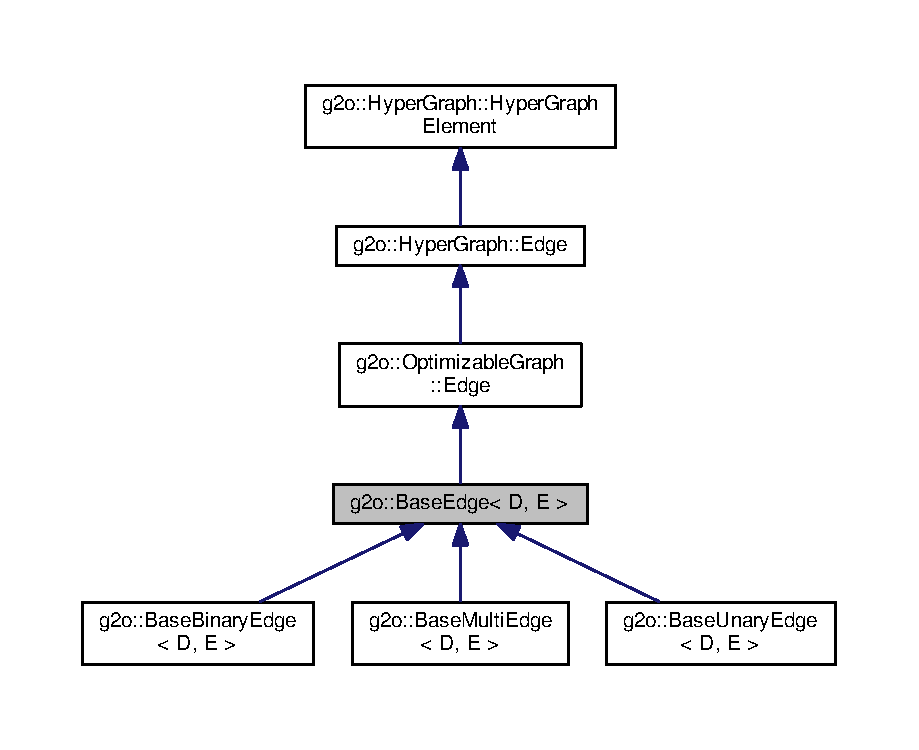
\includegraphics[width=350pt]{classg2o_1_1BaseEdge__inherit__graph}
\end{center}
\end{figure}


g2o\-:\-:Base\-Edge$<$ D, E $>$ 的协作图\-:
\nopagebreak
\begin{figure}[H]
\begin{center}
\leavevmode
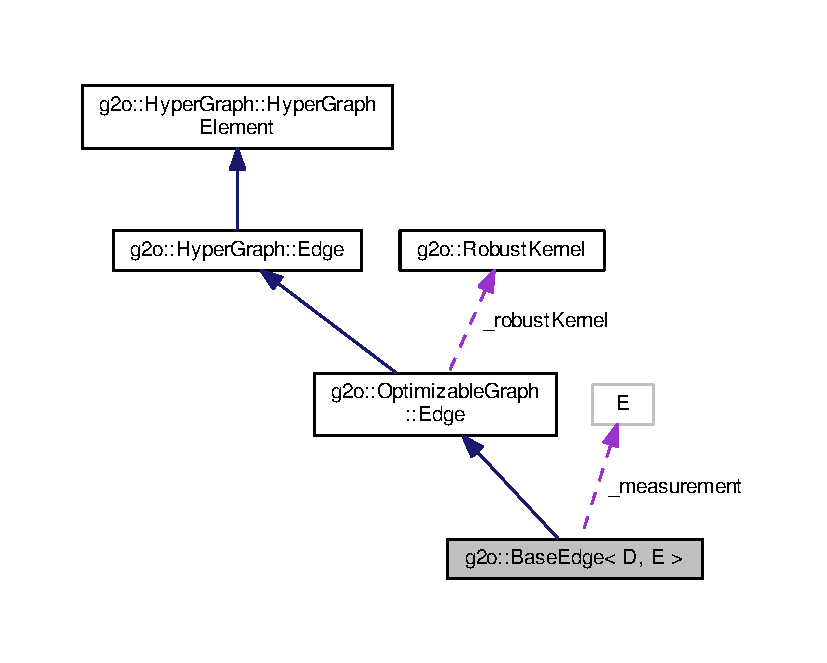
\includegraphics[width=350pt]{classg2o_1_1BaseEdge__coll__graph}
\end{center}
\end{figure}
\subsection*{Public 类型}
\begin{DoxyCompactItemize}
\item 
\hypertarget{classg2o_1_1BaseEdge_a2c148abba650a20b8c7eed75d3e2211e}{typedef E {\bfseries Measurement}}\label{classg2o_1_1BaseEdge_a2c148abba650a20b8c7eed75d3e2211e}

\item 
\hypertarget{classg2o_1_1BaseEdge_af5b558dd24e4be2e437563cae4b3550d}{typedef Matrix$<$ double, D, 1 $>$ {\bfseries Error\-Vector}}\label{classg2o_1_1BaseEdge_af5b558dd24e4be2e437563cae4b3550d}

\item 
\hypertarget{classg2o_1_1BaseEdge_a2e5a33343ac3f189d8a7d5ee4d8b73fc}{typedef Matrix$<$ double, D, D $>$ {\bfseries Information\-Type}}\label{classg2o_1_1BaseEdge_a2e5a33343ac3f189d8a7d5ee4d8b73fc}

\end{DoxyCompactItemize}
\subsection*{Public 成员函数}
\begin{DoxyCompactItemize}
\item 
\hypertarget{classg2o_1_1BaseEdge_a7ea9406b8cc06b44433569bbd4fcefac}{virtual double \hyperlink{classg2o_1_1BaseEdge_a7ea9406b8cc06b44433569bbd4fcefac}{chi2} () const }\label{classg2o_1_1BaseEdge_a7ea9406b8cc06b44433569bbd4fcefac}

\begin{DoxyCompactList}\small\item\em computes the chi2 based on the cached error value, only valid after compute\-Error has been called. \end{DoxyCompactList}\item 
\hypertarget{classg2o_1_1BaseEdge_a2483ee84ebe78e35e71db7dce703edae}{virtual const double $\ast$ \hyperlink{classg2o_1_1BaseEdge_a2483ee84ebe78e35e71db7dce703edae}{error\-Data} () const }\label{classg2o_1_1BaseEdge_a2483ee84ebe78e35e71db7dce703edae}

\begin{DoxyCompactList}\small\item\em returns the error vector cached after calling the compute\-Error; \end{DoxyCompactList}\item 
\hypertarget{classg2o_1_1BaseEdge_ab80452c1134036928a2af6303412a3c4}{virtual double $\ast$ {\bfseries error\-Data} ()}\label{classg2o_1_1BaseEdge_ab80452c1134036928a2af6303412a3c4}

\item 
\hypertarget{classg2o_1_1BaseEdge_a52fb082b224f30a29248431ea34e9c39}{const Error\-Vector \& {\bfseries error} () const }\label{classg2o_1_1BaseEdge_a52fb082b224f30a29248431ea34e9c39}

\item 
\hypertarget{classg2o_1_1BaseEdge_ad0a9e3b6d5490c8f4af794c77742faae}{Error\-Vector \& {\bfseries error} ()}\label{classg2o_1_1BaseEdge_ad0a9e3b6d5490c8f4af794c77742faae}

\item 
\hypertarget{classg2o_1_1BaseEdge_ab682086df7223ce2b039d652416ddc23}{const Information\-Type \& \hyperlink{classg2o_1_1BaseEdge_ab682086df7223ce2b039d652416ddc23}{information} () const }\label{classg2o_1_1BaseEdge_ab682086df7223ce2b039d652416ddc23}

\begin{DoxyCompactList}\small\item\em information matrix of the constraint \end{DoxyCompactList}\item 
\hypertarget{classg2o_1_1BaseEdge_addff9120320d63504e07bfe17f1d04a7}{Information\-Type \& {\bfseries information} ()}\label{classg2o_1_1BaseEdge_addff9120320d63504e07bfe17f1d04a7}

\item 
\hypertarget{classg2o_1_1BaseEdge_a9bb871a94d2413ec3113a147417f2dc4}{void {\bfseries set\-Information} (const Information\-Type \&\hyperlink{classg2o_1_1BaseEdge_ab682086df7223ce2b039d652416ddc23}{information})}\label{classg2o_1_1BaseEdge_a9bb871a94d2413ec3113a147417f2dc4}

\item 
\hypertarget{classg2o_1_1BaseEdge_a49791e1acda790a7819388e60d80ed50}{virtual const double $\ast$ \hyperlink{classg2o_1_1BaseEdge_a49791e1acda790a7819388e60d80ed50}{information\-Data} () const }\label{classg2o_1_1BaseEdge_a49791e1acda790a7819388e60d80ed50}

\begin{DoxyCompactList}\small\item\em returns the memory of the information matrix, usable for example with a Eigen\-::\-Map$<$\-Matrix\-Xd$>$ \end{DoxyCompactList}\item 
\hypertarget{classg2o_1_1BaseEdge_a72ae9d215d6abc892f735e3d3ab81a88}{virtual double $\ast$ {\bfseries information\-Data} ()}\label{classg2o_1_1BaseEdge_a72ae9d215d6abc892f735e3d3ab81a88}

\item 
\hypertarget{classg2o_1_1BaseEdge_a8c20e7ffa66bb7a4a02c8cee82e89c8b}{const Measurement \& \hyperlink{classg2o_1_1BaseEdge_a8c20e7ffa66bb7a4a02c8cee82e89c8b}{measurement} () const }\label{classg2o_1_1BaseEdge_a8c20e7ffa66bb7a4a02c8cee82e89c8b}

\begin{DoxyCompactList}\small\item\em accessor functions for the measurement represented by the edge \end{DoxyCompactList}\item 
\hypertarget{classg2o_1_1BaseEdge_a24aae7b4fc35d311158f104cfdd95aeb}{virtual void {\bfseries set\-Measurement} (const Measurement \&m)}\label{classg2o_1_1BaseEdge_a24aae7b4fc35d311158f104cfdd95aeb}

\item 
\hypertarget{classg2o_1_1BaseEdge_a56269f26521052cf52de8a61c37e4c29}{virtual int {\bfseries rank} () const }\label{classg2o_1_1BaseEdge_a56269f26521052cf52de8a61c37e4c29}

\item 
virtual void \hyperlink{classg2o_1_1BaseEdge_a0c3d9763f1dc504627df75e0f381ca70}{initial\-Estimate} (const Optimizable\-Graph\-::\-Vertex\-Set \&, \hyperlink{classg2o_1_1OptimizableGraph_1_1Vertex}{Optimizable\-Graph\-::\-Vertex} $\ast$)
\end{DoxyCompactItemize}
\subsection*{静态 Public 属性}
\begin{DoxyCompactItemize}
\item 
\hypertarget{classg2o_1_1BaseEdge_ab4812acb21e0b9de80dc6d676e71cb70}{static const int {\bfseries Dimension} = D}\label{classg2o_1_1BaseEdge_ab4812acb21e0b9de80dc6d676e71cb70}

\end{DoxyCompactItemize}
\subsection*{Protected 成员函数}
\begin{DoxyCompactItemize}
\item 
Information\-Type \hyperlink{classg2o_1_1BaseEdge_a069937ed6fadf557368cd0fce7ab2f59}{robust\-Information} (const Eigen\-::\-Vector3d \&rho)
\end{DoxyCompactItemize}
\subsection*{Protected 属性}
\begin{DoxyCompactItemize}
\item 
\hypertarget{classg2o_1_1BaseEdge_af2a6ab1df6e91601b4cab23e0e99e034}{Measurement {\bfseries \-\_\-measurement}}\label{classg2o_1_1BaseEdge_af2a6ab1df6e91601b4cab23e0e99e034}

\item 
\hypertarget{classg2o_1_1BaseEdge_a49f11e3d1eaa8e666e1d4d3607279377}{Information\-Type {\bfseries \-\_\-information}}\label{classg2o_1_1BaseEdge_a49f11e3d1eaa8e666e1d4d3607279377}

\item 
\hypertarget{classg2o_1_1BaseEdge_af31f4b0a67bb12b4de4a32dc42467836}{Error\-Vector {\bfseries \-\_\-error}}\label{classg2o_1_1BaseEdge_af31f4b0a67bb12b4de4a32dc42467836}

\end{DoxyCompactItemize}


\subsection{详细描述}
\subsubsection*{template$<$int D, typename E$>$class g2o\-::\-Base\-Edge$<$ D, E $>$}



在文件 base\-\_\-edge.\-h 第 42 行定义.



\subsection{成员函数说明}
\hypertarget{classg2o_1_1BaseEdge_a0c3d9763f1dc504627df75e0f381ca70}{\index{g2o\-::\-Base\-Edge@{g2o\-::\-Base\-Edge}!initial\-Estimate@{initial\-Estimate}}
\index{initial\-Estimate@{initial\-Estimate}!g2o::BaseEdge@{g2o\-::\-Base\-Edge}}
\subsubsection[{initial\-Estimate}]{\setlength{\rightskip}{0pt plus 5cm}template$<$int D, typename E$>$ virtual void {\bf g2o\-::\-Base\-Edge}$<$ D, E $>$\-::initial\-Estimate (
\begin{DoxyParamCaption}
\item[{const Optimizable\-Graph\-::\-Vertex\-Set \&}]{from, }
\item[{{\bf Optimizable\-Graph\-::\-Vertex} $\ast$}]{to}
\end{DoxyParamCaption}
)\hspace{0.3cm}{\ttfamily [inline]}, {\ttfamily [virtual]}}}\label{classg2o_1_1BaseEdge_a0c3d9763f1dc504627df75e0f381ca70}
set the estimate of the to vertex, based on the estimate of the from vertices in the edge. 

实现了 \hyperlink{classg2o_1_1OptimizableGraph_1_1Edge_a9519f8892e97f03daacb44ea50ac7f4e}{g2o\-::\-Optimizable\-Graph\-::\-Edge}.



被 \hyperlink{classg2o_1_1EdgeSim3_afac4cc093af6f54adb278c142f33dcca}{g2o\-::\-Edge\-Sim3}, \hyperlink{classg2o_1_1BaseUnaryEdge_a3d3311901116092cf817b094f6a0b44b}{g2o\-::\-Base\-Unary\-Edge$<$ D, E, Vertex\-Xi $>$}, \hyperlink{classg2o_1_1BaseUnaryEdge_a3d3311901116092cf817b094f6a0b44b}{g2o\-::\-Base\-Unary\-Edge$<$ 2, Vector2d, Vertex\-S\-E3\-Expmap $>$} , 以及 \hyperlink{classg2o_1_1BaseUnaryEdge_a3d3311901116092cf817b094f6a0b44b}{g2o\-::\-Base\-Unary\-Edge$<$ 3, Vector3d, Vertex\-S\-E3\-Expmap $>$} 重载.



在文件 base\-\_\-edge.\-h 第 82 行定义.

\hypertarget{classg2o_1_1BaseEdge_a069937ed6fadf557368cd0fce7ab2f59}{\index{g2o\-::\-Base\-Edge@{g2o\-::\-Base\-Edge}!robust\-Information@{robust\-Information}}
\index{robust\-Information@{robust\-Information}!g2o::BaseEdge@{g2o\-::\-Base\-Edge}}
\subsubsection[{robust\-Information}]{\setlength{\rightskip}{0pt plus 5cm}template$<$int D, typename E$>$ Information\-Type {\bf g2o\-::\-Base\-Edge}$<$ D, E $>$\-::robust\-Information (
\begin{DoxyParamCaption}
\item[{const Eigen\-::\-Vector3d \&}]{rho}
\end{DoxyParamCaption}
)\hspace{0.3cm}{\ttfamily [inline]}, {\ttfamily [protected]}}}\label{classg2o_1_1BaseEdge_a069937ed6fadf557368cd0fce7ab2f59}
calculate the robust information matrix by updating the information matrix of the error 

在文件 base\-\_\-edge.\-h 第 96 行定义.



该类的文档由以下文件生成\-:\begin{DoxyCompactItemize}
\item 
Thirdparty/g2o/g2o/core/base\-\_\-edge.\-h\end{DoxyCompactItemize}

\hypertarget{classg2o_1_1BaseMultiEdge}{\section{g2o\-:\-:Base\-Multi\-Edge$<$ D, E $>$ 模板类 参考}
\label{classg2o_1_1BaseMultiEdge}\index{g2o\-::\-Base\-Multi\-Edge$<$ D, E $>$@{g2o\-::\-Base\-Multi\-Edge$<$ D, E $>$}}
}


base class to represent an edge connecting an arbitrary number of nodes  




{\ttfamily \#include $<$base\-\_\-multi\-\_\-edge.\-h$>$}



类 g2o\-:\-:Base\-Multi\-Edge$<$ D, E $>$ 继承关系图\-:
\nopagebreak
\begin{figure}[H]
\begin{center}
\leavevmode
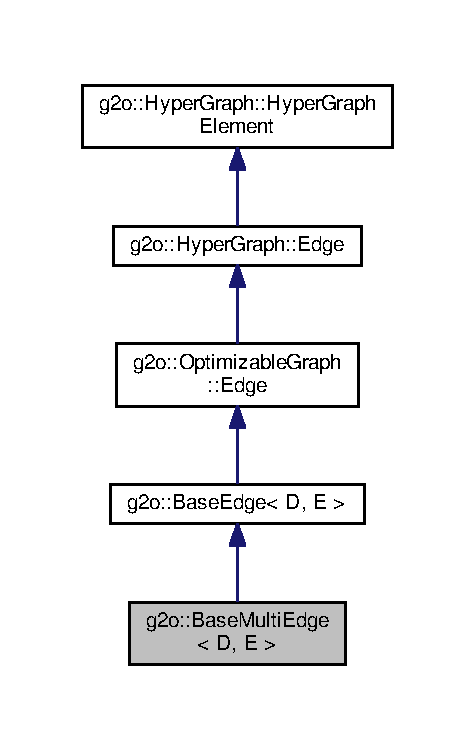
\includegraphics[width=228pt]{classg2o_1_1BaseMultiEdge__inherit__graph}
\end{center}
\end{figure}


g2o\-:\-:Base\-Multi\-Edge$<$ D, E $>$ 的协作图\-:
\nopagebreak
\begin{figure}[H]
\begin{center}
\leavevmode
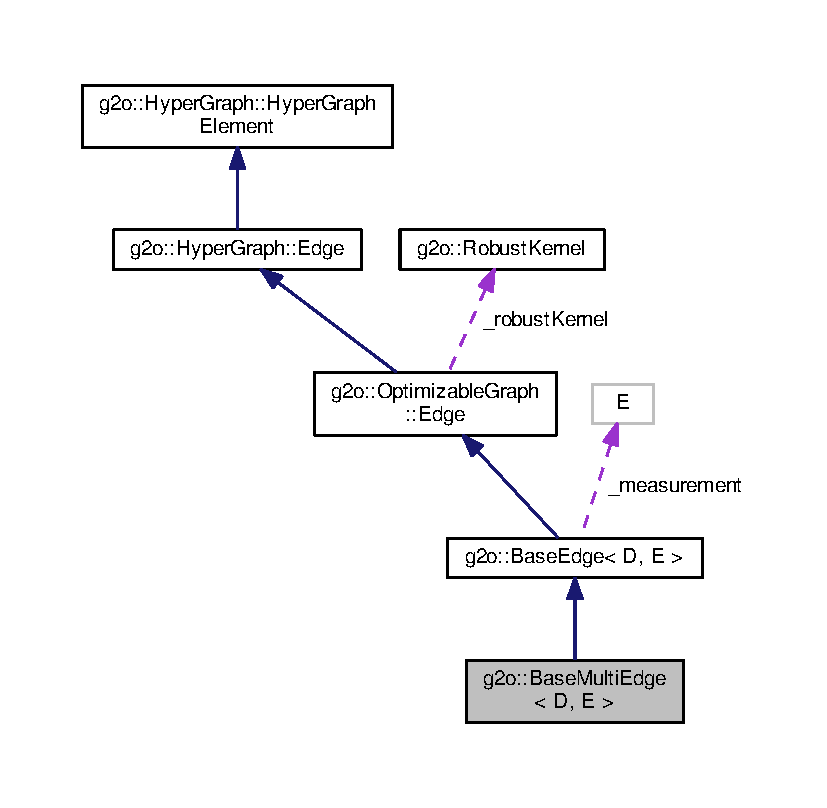
\includegraphics[width=350pt]{classg2o_1_1BaseMultiEdge__coll__graph}
\end{center}
\end{figure}
\subsection*{类}
\begin{DoxyCompactItemize}
\item 
struct \hyperlink{structg2o_1_1BaseMultiEdge_1_1HessianHelper}{Hessian\-Helper}
\begin{DoxyCompactList}\small\item\em helper for mapping the Hessian memory of the upper triangular block \end{DoxyCompactList}\end{DoxyCompactItemize}
\subsection*{Public 类型}
\begin{DoxyCompactItemize}
\item 
\hypertarget{classg2o_1_1BaseMultiEdge_acbaff4c018fb314db5c7852054ffb89d}{typedef \hyperlink{classg2o_1_1BaseEdge}{Base\-Edge}$<$ D, E $>$\\*
\-::Measurement {\bfseries Measurement}}\label{classg2o_1_1BaseMultiEdge_acbaff4c018fb314db5c7852054ffb89d}

\item 
\hypertarget{classg2o_1_1BaseMultiEdge_a43dfdf5b27df296a32ee5a11f0653d55}{typedef Matrix\-Xd\-::\-Map\-Type {\bfseries Jacobian\-Type}}\label{classg2o_1_1BaseMultiEdge_a43dfdf5b27df296a32ee5a11f0653d55}

\item 
\hypertarget{classg2o_1_1BaseMultiEdge_ae17c6b5747bfed295214942207a6eb74}{typedef \hyperlink{classg2o_1_1BaseEdge}{Base\-Edge}$<$ D, E $>$\\*
\-::Error\-Vector {\bfseries Error\-Vector}}\label{classg2o_1_1BaseMultiEdge_ae17c6b5747bfed295214942207a6eb74}

\item 
\hypertarget{classg2o_1_1BaseMultiEdge_a368ab136a2cee049549cb479fb4c88fa}{typedef \hyperlink{classg2o_1_1BaseEdge}{Base\-Edge}$<$ D, E $>$\\*
\-::Information\-Type {\bfseries Information\-Type}}\label{classg2o_1_1BaseMultiEdge_a368ab136a2cee049549cb479fb4c88fa}

\item 
\hypertarget{classg2o_1_1BaseMultiEdge_af299cc8f77d917c1ad4a7d8004aec3a1}{typedef Eigen\-::\-Map$<$ Matrix\-Xd, \\*
Matrix\-Xd\-::\-Flags \&Aligned\-Bit?Aligned\-:\-Unaligned $>$ {\bfseries Hessian\-Block\-Type}}\label{classg2o_1_1BaseMultiEdge_af299cc8f77d917c1ad4a7d8004aec3a1}

\end{DoxyCompactItemize}
\subsection*{Public 成员函数}
\begin{DoxyCompactItemize}
\item 
virtual void \hyperlink{classg2o_1_1BaseMultiEdge_a72176776797987b8ae79ea2e33971e9e}{linearize\-Oplus} (\hyperlink{classg2o_1_1JacobianWorkspace}{Jacobian\-Workspace} \&jacobian\-Workspace)
\item 
virtual void \hyperlink{classg2o_1_1BaseMultiEdge_a6196a4cd1ddc2ef27c1474252bb60e9f}{linearize\-Oplus} ()
\item 
virtual void \hyperlink{classg2o_1_1BaseMultiEdge_ae07ec9359cd515d0abc2100ee8aae93f}{resize} (size\-\_\-t size)
\item 
\hypertarget{classg2o_1_1BaseMultiEdge_a0873441402f991c0cfbe92a6ab718daa}{virtual bool {\bfseries all\-Vertices\-Fixed} () const }\label{classg2o_1_1BaseMultiEdge_a0873441402f991c0cfbe92a6ab718daa}

\item 
virtual void \hyperlink{classg2o_1_1BaseMultiEdge_ae44ba0385d4dda4bc038d81e50cadd8c}{construct\-Quadratic\-Form} ()
\item 
virtual void \hyperlink{classg2o_1_1BaseMultiEdge_aecded66022b967fab0deb1c6a2d76445}{map\-Hessian\-Memory} (double $\ast$d, int i, int j, bool row\-Major)
\end{DoxyCompactItemize}
\subsection*{静态 Public 属性}
\begin{DoxyCompactItemize}
\item 
\hypertarget{classg2o_1_1BaseMultiEdge_a3c713fe8d1cd161f777625d8e2d5695d}{static const int {\bfseries Dimension} = \hyperlink{classg2o_1_1BaseEdge}{Base\-Edge}$<$D,E$>$\-::Dimension}\label{classg2o_1_1BaseMultiEdge_a3c713fe8d1cd161f777625d8e2d5695d}

\end{DoxyCompactItemize}
\subsection*{Protected 成员函数}
\begin{DoxyCompactItemize}
\item 
\hypertarget{classg2o_1_1BaseMultiEdge_ac260b65c12f6594165af680f815ac291}{void {\bfseries compute\-Quadratic\-Form} (const Information\-Type \&omega, const Error\-Vector \&weighted\-Error)}\label{classg2o_1_1BaseMultiEdge_ac260b65c12f6594165af680f815ac291}

\end{DoxyCompactItemize}
\subsection*{Protected 属性}
\begin{DoxyCompactItemize}
\item 
\hypertarget{classg2o_1_1BaseMultiEdge_af927d6f41bf73fc3b928cae2d6219d9e}{std\-::vector$<$ \hyperlink{structg2o_1_1BaseMultiEdge_1_1HessianHelper}{Hessian\-Helper} $>$ {\bfseries \-\_\-hessian}}\label{classg2o_1_1BaseMultiEdge_af927d6f41bf73fc3b928cae2d6219d9e}

\item 
\hypertarget{classg2o_1_1BaseMultiEdge_a00f8130e287bc945a8436375c4d07a02}{std\-::vector$<$ Jacobian\-Type, \\*
aligned\-\_\-allocator\\*
$<$ Jacobian\-Type $>$ $>$ \hyperlink{classg2o_1_1BaseMultiEdge_a00f8130e287bc945a8436375c4d07a02}{\-\_\-jacobian\-Oplus}}\label{classg2o_1_1BaseMultiEdge_a00f8130e287bc945a8436375c4d07a02}

\begin{DoxyCompactList}\small\item\em jacobians of the edge (w.\-r.\-t. oplus) \end{DoxyCompactList}\end{DoxyCompactItemize}


\subsection{详细描述}
\subsubsection*{template$<$int D, typename E$>$class g2o\-::\-Base\-Multi\-Edge$<$ D, E $>$}

base class to represent an edge connecting an arbitrary number of nodes 

D -\/ Dimension of the measurement E -\/ type to represent the measurement 

在文件 base\-\_\-multi\-\_\-edge.\-h 第 51 行定义.



\subsection{成员函数说明}
\hypertarget{classg2o_1_1BaseMultiEdge_ae44ba0385d4dda4bc038d81e50cadd8c}{\index{g2o\-::\-Base\-Multi\-Edge@{g2o\-::\-Base\-Multi\-Edge}!construct\-Quadratic\-Form@{construct\-Quadratic\-Form}}
\index{construct\-Quadratic\-Form@{construct\-Quadratic\-Form}!g2o::BaseMultiEdge@{g2o\-::\-Base\-Multi\-Edge}}
\subsubsection[{construct\-Quadratic\-Form}]{\setlength{\rightskip}{0pt plus 5cm}template$<$int D, typename E $>$ void Base\-Multi\-Edge\-::construct\-Quadratic\-Form (
\begin{DoxyParamCaption}
{}
\end{DoxyParamCaption}
)\hspace{0.3cm}{\ttfamily [virtual]}}}\label{classg2o_1_1BaseMultiEdge_ae44ba0385d4dda4bc038d81e50cadd8c}
Linearizes the constraint in the edge. Makes side effect on the vertices of the graph by changing the parameter vector b and the hessian blocks ii and jj. The off diagoinal block is accesed via \-\_\-hessian. 

实现了 \hyperlink{classg2o_1_1OptimizableGraph_1_1Edge_a56fbf3430ddf591e3c619bdd1b7e4499}{g2o\-::\-Optimizable\-Graph\-::\-Edge}.



在文件 base\-\_\-multi\-\_\-edge.\-h 第 37 行定义.

\hypertarget{classg2o_1_1BaseMultiEdge_a72176776797987b8ae79ea2e33971e9e}{\index{g2o\-::\-Base\-Multi\-Edge@{g2o\-::\-Base\-Multi\-Edge}!linearize\-Oplus@{linearize\-Oplus}}
\index{linearize\-Oplus@{linearize\-Oplus}!g2o::BaseMultiEdge@{g2o\-::\-Base\-Multi\-Edge}}
\subsubsection[{linearize\-Oplus}]{\setlength{\rightskip}{0pt plus 5cm}template$<$int D, typename E $>$ void Base\-Multi\-Edge\-::linearize\-Oplus (
\begin{DoxyParamCaption}
\item[{{\bf Jacobian\-Workspace} \&}]{jacobian\-Workspace}
\end{DoxyParamCaption}
)\hspace{0.3cm}{\ttfamily [virtual]}}}\label{classg2o_1_1BaseMultiEdge_a72176776797987b8ae79ea2e33971e9e}
Linearizes the constraint in the edge in the manifold space, and store the result in the given workspace 

实现了 \hyperlink{classg2o_1_1OptimizableGraph_1_1Edge_a0fdad5ebfb4efec9f893b57f67e0fbe1}{g2o\-::\-Optimizable\-Graph\-::\-Edge}.



在文件 base\-\_\-multi\-\_\-edge.\-h 第 53 行定义.

\hypertarget{classg2o_1_1BaseMultiEdge_a6196a4cd1ddc2ef27c1474252bb60e9f}{\index{g2o\-::\-Base\-Multi\-Edge@{g2o\-::\-Base\-Multi\-Edge}!linearize\-Oplus@{linearize\-Oplus}}
\index{linearize\-Oplus@{linearize\-Oplus}!g2o::BaseMultiEdge@{g2o\-::\-Base\-Multi\-Edge}}
\subsubsection[{linearize\-Oplus}]{\setlength{\rightskip}{0pt plus 5cm}template$<$int D, typename E $>$ void Base\-Multi\-Edge\-::linearize\-Oplus (
\begin{DoxyParamCaption}
{}
\end{DoxyParamCaption}
)\hspace{0.3cm}{\ttfamily [virtual]}}}\label{classg2o_1_1BaseMultiEdge_a6196a4cd1ddc2ef27c1474252bb60e9f}
Linearizes the oplus operator in the vertex, and stores the result in temporary variable vector \-\_\-jacobian\-Oplus 

在文件 base\-\_\-multi\-\_\-edge.\-h 第 64 行定义.

\hypertarget{classg2o_1_1BaseMultiEdge_aecded66022b967fab0deb1c6a2d76445}{\index{g2o\-::\-Base\-Multi\-Edge@{g2o\-::\-Base\-Multi\-Edge}!map\-Hessian\-Memory@{map\-Hessian\-Memory}}
\index{map\-Hessian\-Memory@{map\-Hessian\-Memory}!g2o::BaseMultiEdge@{g2o\-::\-Base\-Multi\-Edge}}
\subsubsection[{map\-Hessian\-Memory}]{\setlength{\rightskip}{0pt plus 5cm}template$<$int D, typename E $>$ void Base\-Multi\-Edge\-::map\-Hessian\-Memory (
\begin{DoxyParamCaption}
\item[{double $\ast$}]{d, }
\item[{int}]{i, }
\item[{int}]{j, }
\item[{bool}]{row\-Major}
\end{DoxyParamCaption}
)\hspace{0.3cm}{\ttfamily [virtual]}}}\label{classg2o_1_1BaseMultiEdge_aecded66022b967fab0deb1c6a2d76445}
maps the internal matrix to some external memory location, you need to provide the memory before calling construct\-Quadratic\-Form 
\begin{DoxyParams}{参数}
{\em d} & the memory location to which we map \\
\hline
{\em i} & index of the vertex i \\
\hline
{\em j} & index of the vertex j (j $>$ i, upper triangular fashion) \\
\hline
{\em row\-Major} & if true, will write in row\-Major order to the block. Since E\-I\-G\-E\-N is column\-Major by default, this results in writing the transposed \\
\hline
\end{DoxyParams}


实现了 \hyperlink{classg2o_1_1OptimizableGraph_1_1Edge_a3bd233fd552daa166039acf47b69a5a7}{g2o\-::\-Optimizable\-Graph\-::\-Edge}.



在文件 base\-\_\-multi\-\_\-edge.\-h 第 130 行定义.

\hypertarget{classg2o_1_1BaseMultiEdge_ae07ec9359cd515d0abc2100ee8aae93f}{\index{g2o\-::\-Base\-Multi\-Edge@{g2o\-::\-Base\-Multi\-Edge}!resize@{resize}}
\index{resize@{resize}!g2o::BaseMultiEdge@{g2o\-::\-Base\-Multi\-Edge}}
\subsubsection[{resize}]{\setlength{\rightskip}{0pt plus 5cm}template$<$int D, typename E $>$ void Base\-Multi\-Edge\-::resize (
\begin{DoxyParamCaption}
\item[{size\-\_\-t}]{size}
\end{DoxyParamCaption}
)\hspace{0.3cm}{\ttfamily [virtual]}}}\label{classg2o_1_1BaseMultiEdge_ae07ec9359cd515d0abc2100ee8aae93f}
resizes the number of vertices connected by this edge 

重载 \hyperlink{classg2o_1_1HyperGraph_1_1Edge_ad8913f1149a0fd5bb628f0f1c8a91a55}{g2o\-::\-Hyper\-Graph\-::\-Edge} .



在文件 base\-\_\-multi\-\_\-edge.\-h 第 150 行定义.



该类的文档由以下文件生成\-:\begin{DoxyCompactItemize}
\item 
Thirdparty/g2o/g2o/core/base\-\_\-multi\-\_\-edge.\-h\item 
Thirdparty/g2o/g2o/core/base\-\_\-multi\-\_\-edge.\-hpp\end{DoxyCompactItemize}

\hypertarget{classg2o_1_1BaseProperty}{\section{g2o\-:\-:Base\-Property类 参考}
\label{classg2o_1_1BaseProperty}\index{g2o\-::\-Base\-Property@{g2o\-::\-Base\-Property}}
}


类 g2o\-:\-:Base\-Property 继承关系图\-:
\nopagebreak
\begin{figure}[H]
\begin{center}
\leavevmode
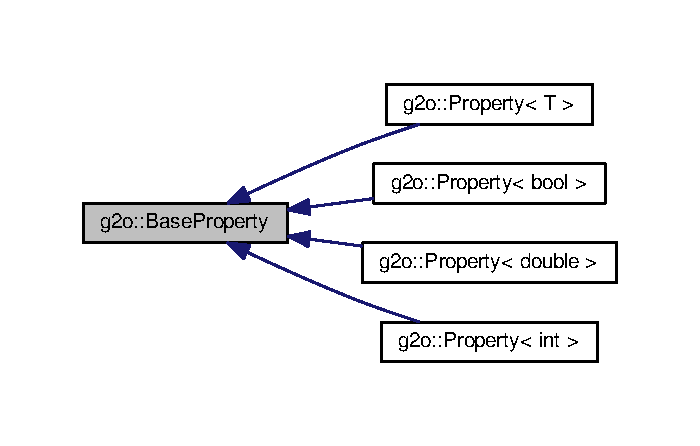
\includegraphics[width=336pt]{classg2o_1_1BaseProperty__inherit__graph}
\end{center}
\end{figure}
\subsection*{Public 成员函数}
\begin{DoxyCompactItemize}
\item 
\hypertarget{classg2o_1_1BaseProperty_a00444ab7926d86beb9e66550e40e5d97}{{\bfseries Base\-Property} (const std\-::string name\-\_\-)}\label{classg2o_1_1BaseProperty_a00444ab7926d86beb9e66550e40e5d97}

\item 
\hypertarget{classg2o_1_1BaseProperty_aae91313b0eb376dd9460cd712ecbb86d}{const std\-::string \& {\bfseries name} ()}\label{classg2o_1_1BaseProperty_aae91313b0eb376dd9460cd712ecbb86d}

\item 
\hypertarget{classg2o_1_1BaseProperty_a7a4191088468c2f03dab52107d130833}{virtual std\-::string {\bfseries to\-String} () const =0}\label{classg2o_1_1BaseProperty_a7a4191088468c2f03dab52107d130833}

\item 
\hypertarget{classg2o_1_1BaseProperty_aeabc313d9f66a403738aece884c85e1d}{virtual bool {\bfseries from\-String} (const std\-::string \&s)=0}\label{classg2o_1_1BaseProperty_aeabc313d9f66a403738aece884c85e1d}

\end{DoxyCompactItemize}
\subsection*{Protected 属性}
\begin{DoxyCompactItemize}
\item 
\hypertarget{classg2o_1_1BaseProperty_a74e4bbf35ddf26022cb39be2ea7abd2b}{std\-::string {\bfseries \-\_\-name}}\label{classg2o_1_1BaseProperty_a74e4bbf35ddf26022cb39be2ea7abd2b}

\end{DoxyCompactItemize}


\subsection{详细描述}


在文件 property.\-h 第 39 行定义.



该类的文档由以下文件生成\-:\begin{DoxyCompactItemize}
\item 
Thirdparty/g2o/g2o/stuff/property.\-h\item 
Thirdparty/g2o/g2o/stuff/property.\-cpp\end{DoxyCompactItemize}

\hypertarget{classg2o_1_1BaseUnaryEdge}{\section{g2o\-:\-:Base\-Unary\-Edge$<$ D, E, Vertex\-Xi $>$ 模板类 参考}
\label{classg2o_1_1BaseUnaryEdge}\index{g2o\-::\-Base\-Unary\-Edge$<$ D, E, Vertex\-Xi $>$@{g2o\-::\-Base\-Unary\-Edge$<$ D, E, Vertex\-Xi $>$}}
}


类 g2o\-:\-:Base\-Unary\-Edge$<$ D, E, Vertex\-Xi $>$ 继承关系图\-:
\nopagebreak
\begin{figure}[H]
\begin{center}
\leavevmode
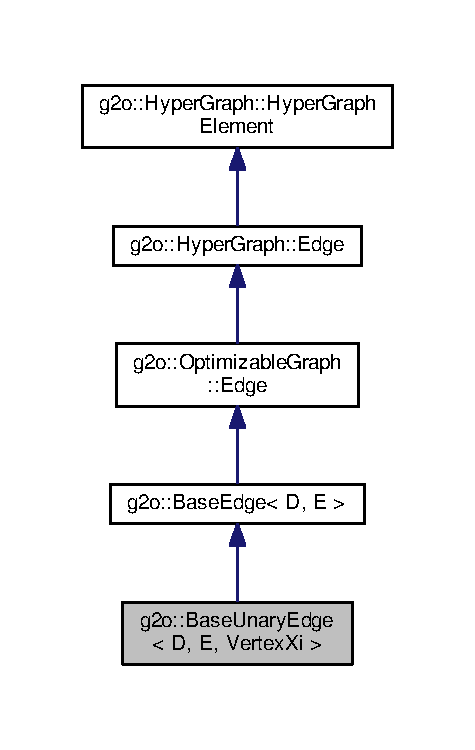
\includegraphics[width=228pt]{classg2o_1_1BaseUnaryEdge__inherit__graph}
\end{center}
\end{figure}


g2o\-:\-:Base\-Unary\-Edge$<$ D, E, Vertex\-Xi $>$ 的协作图\-:
\nopagebreak
\begin{figure}[H]
\begin{center}
\leavevmode
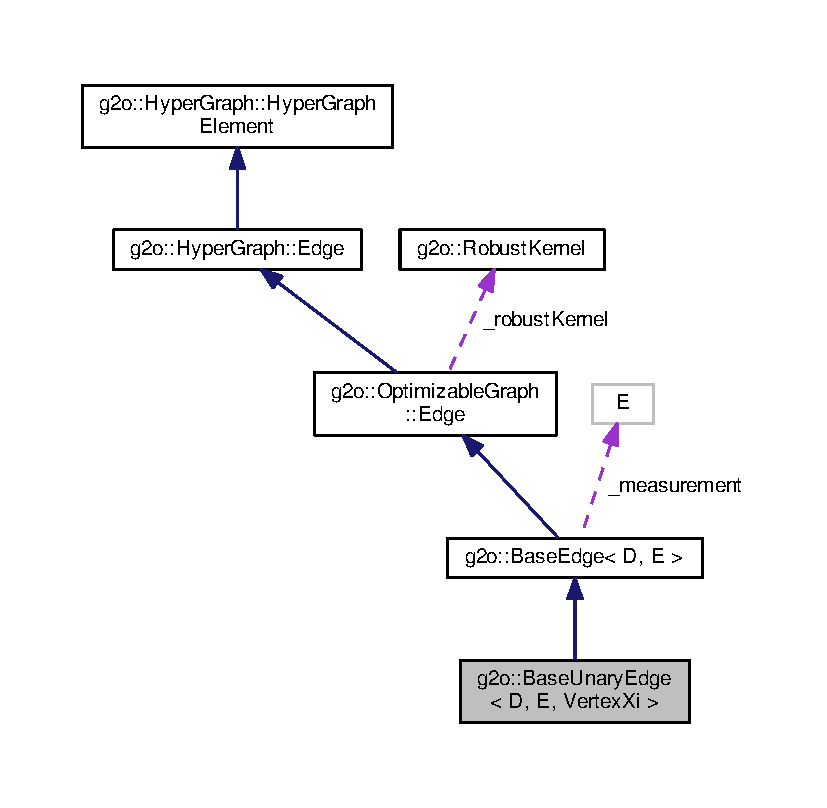
\includegraphics[width=350pt]{classg2o_1_1BaseUnaryEdge__coll__graph}
\end{center}
\end{figure}
\subsection*{Public 类型}
\begin{DoxyCompactItemize}
\item 
\hypertarget{classg2o_1_1BaseUnaryEdge_ab953b076b4c35fcf99de02bd0bfcc1ae}{typedef \hyperlink{classg2o_1_1BaseEdge}{Base\-Edge}$<$ D, E $>$\\*
\-::Measurement {\bfseries Measurement}}\label{classg2o_1_1BaseUnaryEdge_ab953b076b4c35fcf99de02bd0bfcc1ae}

\item 
\hypertarget{classg2o_1_1BaseUnaryEdge_a503e62e74775172c008135650850d511}{typedef Vertex\-Xi {\bfseries Vertex\-Xi\-Type}}\label{classg2o_1_1BaseUnaryEdge_a503e62e74775172c008135650850d511}

\item 
\hypertarget{classg2o_1_1BaseUnaryEdge_a24bcabd661223e15b7337f2835310f5e}{typedef Matrix$<$ double, D, \\*
Vertex\-Xi\-Type\-::\-Dimension $>$\\*
\-::Aligned\-Map\-Type {\bfseries Jacobian\-Xi\-Oplus\-Type}}\label{classg2o_1_1BaseUnaryEdge_a24bcabd661223e15b7337f2835310f5e}

\item 
\hypertarget{classg2o_1_1BaseUnaryEdge_abc04cfacb65fc72825156f1b3346dd48}{typedef \hyperlink{classg2o_1_1BaseEdge}{Base\-Edge}$<$ D, E $>$\\*
\-::Error\-Vector {\bfseries Error\-Vector}}\label{classg2o_1_1BaseUnaryEdge_abc04cfacb65fc72825156f1b3346dd48}

\item 
\hypertarget{classg2o_1_1BaseUnaryEdge_a6753caa95c30fa5bb3887e2a30892ff3}{typedef \hyperlink{classg2o_1_1BaseEdge}{Base\-Edge}$<$ D, E $>$\\*
\-::Information\-Type {\bfseries Information\-Type}}\label{classg2o_1_1BaseUnaryEdge_a6753caa95c30fa5bb3887e2a30892ff3}

\end{DoxyCompactItemize}
\subsection*{Public 成员函数}
\begin{DoxyCompactItemize}
\item 
virtual void \hyperlink{classg2o_1_1BaseUnaryEdge_a01fcdfd2d3ed0325655bb99db95c0b10}{resize} (size\-\_\-t size)
\item 
\hypertarget{classg2o_1_1BaseUnaryEdge_ae3db6c719eac18fce051b40a8c8b86dd}{virtual bool {\bfseries all\-Vertices\-Fixed} () const }\label{classg2o_1_1BaseUnaryEdge_ae3db6c719eac18fce051b40a8c8b86dd}

\item 
virtual void \hyperlink{classg2o_1_1BaseUnaryEdge_a8b396647b5b438d30a04758023baa595}{linearize\-Oplus} (\hyperlink{classg2o_1_1JacobianWorkspace}{Jacobian\-Workspace} \&jacobian\-Workspace)
\item 
virtual void \hyperlink{classg2o_1_1BaseUnaryEdge_a367f19b903938faf6e89dd1b0e4e722b}{linearize\-Oplus} ()
\item 
\hypertarget{classg2o_1_1BaseUnaryEdge_a39a254035af4f53fc3a6b5a77cd5a0ca}{const Jacobian\-Xi\-Oplus\-Type \& \hyperlink{classg2o_1_1BaseUnaryEdge_a39a254035af4f53fc3a6b5a77cd5a0ca}{jacobian\-Oplus\-Xi} () const }\label{classg2o_1_1BaseUnaryEdge_a39a254035af4f53fc3a6b5a77cd5a0ca}

\begin{DoxyCompactList}\small\item\em returns the result of the linearization in the manifold space for the node xi \end{DoxyCompactList}\item 
virtual void \hyperlink{classg2o_1_1BaseUnaryEdge_ad7e6dc44c571be159f066bdb961ade2b}{construct\-Quadratic\-Form} ()
\item 
virtual void \hyperlink{classg2o_1_1BaseUnaryEdge_a3d3311901116092cf817b094f6a0b44b}{initial\-Estimate} (const Optimizable\-Graph\-::\-Vertex\-Set \&from, \hyperlink{classg2o_1_1OptimizableGraph_1_1Vertex}{Optimizable\-Graph\-::\-Vertex} $\ast$to)
\item 
virtual void \hyperlink{classg2o_1_1BaseUnaryEdge_a919dcb89130f6e7082e807530facdd78}{map\-Hessian\-Memory} (double $\ast$, int, int, bool)
\end{DoxyCompactItemize}
\subsection*{静态 Public 属性}
\begin{DoxyCompactItemize}
\item 
\hypertarget{classg2o_1_1BaseUnaryEdge_a4e584cf552998a34948d8d5b484f7fd3}{static const int {\bfseries Dimension} = \hyperlink{classg2o_1_1BaseEdge}{Base\-Edge}$<$D, E$>$\-::Dimension}\label{classg2o_1_1BaseUnaryEdge_a4e584cf552998a34948d8d5b484f7fd3}

\end{DoxyCompactItemize}
\subsection*{Protected 属性}
\begin{DoxyCompactItemize}
\item 
\hypertarget{classg2o_1_1BaseUnaryEdge_af7d022a6c6c9c29dfd9147fce0dc13d8}{Jacobian\-Xi\-Oplus\-Type {\bfseries \-\_\-jacobian\-Oplus\-Xi}}\label{classg2o_1_1BaseUnaryEdge_af7d022a6c6c9c29dfd9147fce0dc13d8}

\end{DoxyCompactItemize}
\subsection*{额外继承的成员函数}


\subsection{详细描述}
\subsubsection*{template$<$int D, typename E, typename Vertex\-Xi$>$class g2o\-::\-Base\-Unary\-Edge$<$ D, E, Vertex\-Xi $>$}



在文件 base\-\_\-unary\-\_\-edge.\-h 第 43 行定义.



\subsection{成员函数说明}
\hypertarget{classg2o_1_1BaseUnaryEdge_ad7e6dc44c571be159f066bdb961ade2b}{\index{g2o\-::\-Base\-Unary\-Edge@{g2o\-::\-Base\-Unary\-Edge}!construct\-Quadratic\-Form@{construct\-Quadratic\-Form}}
\index{construct\-Quadratic\-Form@{construct\-Quadratic\-Form}!g2o::BaseUnaryEdge@{g2o\-::\-Base\-Unary\-Edge}}
\subsubsection[{construct\-Quadratic\-Form}]{\setlength{\rightskip}{0pt plus 5cm}template$<$int D, typename E , typename Vertex\-Xi\-Type $>$ void Base\-Unary\-Edge\-::construct\-Quadratic\-Form (
\begin{DoxyParamCaption}
{}
\end{DoxyParamCaption}
)\hspace{0.3cm}{\ttfamily [virtual]}}}\label{classg2o_1_1BaseUnaryEdge_ad7e6dc44c571be159f066bdb961ade2b}
Linearizes the constraint in the edge. Makes side effect on the vertices of the graph by changing the parameter vector b and the hessian blocks ii and jj. The off diagoinal block is accesed via \-\_\-hessian. 

实现了 \hyperlink{classg2o_1_1OptimizableGraph_1_1Edge_a56fbf3430ddf591e3c619bdd1b7e4499}{g2o\-::\-Optimizable\-Graph\-::\-Edge}.



在文件 base\-\_\-unary\-\_\-edge.\-h 第 44 行定义.



参考 g2o\-::\-Hyper\-Graph\-::\-Edge\-::resize().



函数调用图\-:
\nopagebreak
\begin{figure}[H]
\begin{center}
\leavevmode
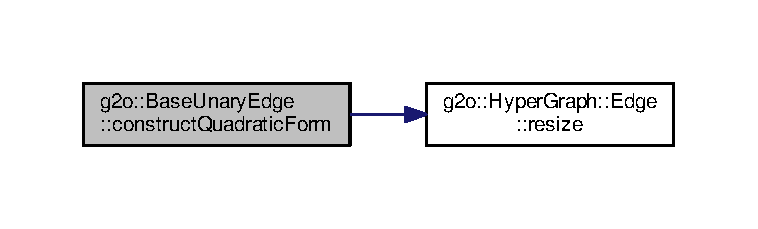
\includegraphics[width=350pt]{classg2o_1_1BaseUnaryEdge_ad7e6dc44c571be159f066bdb961ade2b_cgraph}
\end{center}
\end{figure}


\hypertarget{classg2o_1_1BaseUnaryEdge_a3d3311901116092cf817b094f6a0b44b}{\index{g2o\-::\-Base\-Unary\-Edge@{g2o\-::\-Base\-Unary\-Edge}!initial\-Estimate@{initial\-Estimate}}
\index{initial\-Estimate@{initial\-Estimate}!g2o::BaseUnaryEdge@{g2o\-::\-Base\-Unary\-Edge}}
\subsubsection[{initial\-Estimate}]{\setlength{\rightskip}{0pt plus 5cm}template$<$int D, typename E , typename Vertex\-Xi\-Type $>$ void Base\-Unary\-Edge\-::initial\-Estimate (
\begin{DoxyParamCaption}
\item[{const Optimizable\-Graph\-::\-Vertex\-Set \&}]{from, }
\item[{{\bf Optimizable\-Graph\-::\-Vertex} $\ast$}]{to}
\end{DoxyParamCaption}
)\hspace{0.3cm}{\ttfamily [virtual]}}}\label{classg2o_1_1BaseUnaryEdge_a3d3311901116092cf817b094f6a0b44b}
set the estimate of the to vertex, based on the estimate of the from vertices in the edge. 

重载 \hyperlink{classg2o_1_1BaseEdge_a0c3d9763f1dc504627df75e0f381ca70}{g2o\-::\-Base\-Edge$<$ D, E $>$} .



在文件 base\-\_\-unary\-\_\-edge.\-h 第 127 行定义.

\hypertarget{classg2o_1_1BaseUnaryEdge_a8b396647b5b438d30a04758023baa595}{\index{g2o\-::\-Base\-Unary\-Edge@{g2o\-::\-Base\-Unary\-Edge}!linearize\-Oplus@{linearize\-Oplus}}
\index{linearize\-Oplus@{linearize\-Oplus}!g2o::BaseUnaryEdge@{g2o\-::\-Base\-Unary\-Edge}}
\subsubsection[{linearize\-Oplus}]{\setlength{\rightskip}{0pt plus 5cm}template$<$int D, typename E , typename Vertex\-Xi\-Type $>$ void Base\-Unary\-Edge\-::linearize\-Oplus (
\begin{DoxyParamCaption}
\item[{{\bf Jacobian\-Workspace} \&}]{jacobian\-Workspace}
\end{DoxyParamCaption}
)\hspace{0.3cm}{\ttfamily [virtual]}}}\label{classg2o_1_1BaseUnaryEdge_a8b396647b5b438d30a04758023baa595}
Linearizes the constraint in the edge in the manifold space, and store the result in the given workspace 

实现了 \hyperlink{classg2o_1_1OptimizableGraph_1_1Edge_a0fdad5ebfb4efec9f893b57f67e0fbe1}{g2o\-::\-Optimizable\-Graph\-::\-Edge}.



在文件 base\-\_\-unary\-\_\-edge.\-h 第 76 行定义.

\hypertarget{classg2o_1_1BaseUnaryEdge_a367f19b903938faf6e89dd1b0e4e722b}{\index{g2o\-::\-Base\-Unary\-Edge@{g2o\-::\-Base\-Unary\-Edge}!linearize\-Oplus@{linearize\-Oplus}}
\index{linearize\-Oplus@{linearize\-Oplus}!g2o::BaseUnaryEdge@{g2o\-::\-Base\-Unary\-Edge}}
\subsubsection[{linearize\-Oplus}]{\setlength{\rightskip}{0pt plus 5cm}template$<$int D, typename E , typename Vertex\-Xi\-Type $>$ void Base\-Unary\-Edge\-::linearize\-Oplus (
\begin{DoxyParamCaption}
{}
\end{DoxyParamCaption}
)\hspace{0.3cm}{\ttfamily [virtual]}}}\label{classg2o_1_1BaseUnaryEdge_a367f19b903938faf6e89dd1b0e4e722b}
Linearizes the oplus operator in the vertex, and stores the result in temporary variables \-\_\-jacobian\-Oplus\-Xi and \-\_\-jacobian\-Oplus\-Xj 

被 \hyperlink{classg2o_1_1EdgeStereoSE3ProjectXYZOnlyPose_a0b2b815e8ae331276f33be374dcc1897}{g2o\-::\-Edge\-Stereo\-S\-E3\-Project\-X\-Y\-Z\-Only\-Pose} , 以及 \hyperlink{classg2o_1_1EdgeSE3ProjectXYZOnlyPose_abe6d775aade1277786274c328aa2c38b}{g2o\-::\-Edge\-S\-E3\-Project\-X\-Y\-Z\-Only\-Pose} 重载.



在文件 base\-\_\-unary\-\_\-edge.\-h 第 83 行定义.

\hypertarget{classg2o_1_1BaseUnaryEdge_a919dcb89130f6e7082e807530facdd78}{\index{g2o\-::\-Base\-Unary\-Edge@{g2o\-::\-Base\-Unary\-Edge}!map\-Hessian\-Memory@{map\-Hessian\-Memory}}
\index{map\-Hessian\-Memory@{map\-Hessian\-Memory}!g2o::BaseUnaryEdge@{g2o\-::\-Base\-Unary\-Edge}}
\subsubsection[{map\-Hessian\-Memory}]{\setlength{\rightskip}{0pt plus 5cm}template$<$int D, typename E, typename Vertex\-Xi$>$ virtual void {\bf g2o\-::\-Base\-Unary\-Edge}$<$ D, E, Vertex\-Xi $>$\-::map\-Hessian\-Memory (
\begin{DoxyParamCaption}
\item[{double $\ast$}]{d, }
\item[{int}]{i, }
\item[{int}]{j, }
\item[{bool}]{row\-Major}
\end{DoxyParamCaption}
)\hspace{0.3cm}{\ttfamily [inline]}, {\ttfamily [virtual]}}}\label{classg2o_1_1BaseUnaryEdge_a919dcb89130f6e7082e807530facdd78}
maps the internal matrix to some external memory location, you need to provide the memory before calling construct\-Quadratic\-Form 
\begin{DoxyParams}{参数}
{\em d} & the memory location to which we map \\
\hline
{\em i} & index of the vertex i \\
\hline
{\em j} & index of the vertex j (j $>$ i, upper triangular fashion) \\
\hline
{\em row\-Major} & if true, will write in row\-Major order to the block. Since E\-I\-G\-E\-N is column\-Major by default, this results in writing the transposed \\
\hline
\end{DoxyParams}


实现了 \hyperlink{classg2o_1_1OptimizableGraph_1_1Edge_a3bd233fd552daa166039acf47b69a5a7}{g2o\-::\-Optimizable\-Graph\-::\-Edge}.



在文件 base\-\_\-unary\-\_\-edge.\-h 第 78 行定义.

\hypertarget{classg2o_1_1BaseUnaryEdge_a01fcdfd2d3ed0325655bb99db95c0b10}{\index{g2o\-::\-Base\-Unary\-Edge@{g2o\-::\-Base\-Unary\-Edge}!resize@{resize}}
\index{resize@{resize}!g2o::BaseUnaryEdge@{g2o\-::\-Base\-Unary\-Edge}}
\subsubsection[{resize}]{\setlength{\rightskip}{0pt plus 5cm}template$<$int D, typename E , typename Vertex\-Xi\-Type $>$ void Base\-Unary\-Edge\-::resize (
\begin{DoxyParamCaption}
\item[{size\-\_\-t}]{size}
\end{DoxyParamCaption}
)\hspace{0.3cm}{\ttfamily [virtual]}}}\label{classg2o_1_1BaseUnaryEdge_a01fcdfd2d3ed0325655bb99db95c0b10}
resizes the number of vertices connected by this edge 

重载 \hyperlink{classg2o_1_1HyperGraph_1_1Edge_ad8913f1149a0fd5bb628f0f1c8a91a55}{g2o\-::\-Hyper\-Graph\-::\-Edge} .



在文件 base\-\_\-unary\-\_\-edge.\-h 第 29 行定义.



该类的文档由以下文件生成\-:\begin{DoxyCompactItemize}
\item 
Thirdparty/g2o/g2o/core/base\-\_\-unary\-\_\-edge.\-h\item 
Thirdparty/g2o/g2o/core/base\-\_\-unary\-\_\-edge.\-hpp\end{DoxyCompactItemize}

\hypertarget{classg2o_1_1BaseVertex}{\section{g2o\-:\-:Base\-Vertex$<$ D, T $>$ 模板类 参考}
\label{classg2o_1_1BaseVertex}\index{g2o\-::\-Base\-Vertex$<$ D, T $>$@{g2o\-::\-Base\-Vertex$<$ D, T $>$}}
}


Templatized \hyperlink{classg2o_1_1BaseVertex}{Base\-Vertex}.  




{\ttfamily \#include $<$base\-\_\-vertex.\-h$>$}



类 g2o\-:\-:Base\-Vertex$<$ D, T $>$ 继承关系图\-:
\nopagebreak
\begin{figure}[H]
\begin{center}
\leavevmode
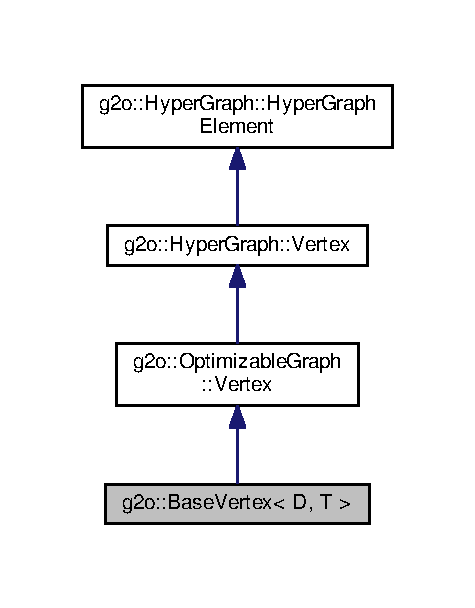
\includegraphics[width=228pt]{classg2o_1_1BaseVertex__inherit__graph}
\end{center}
\end{figure}


g2o\-:\-:Base\-Vertex$<$ D, T $>$ 的协作图\-:
\nopagebreak
\begin{figure}[H]
\begin{center}
\leavevmode
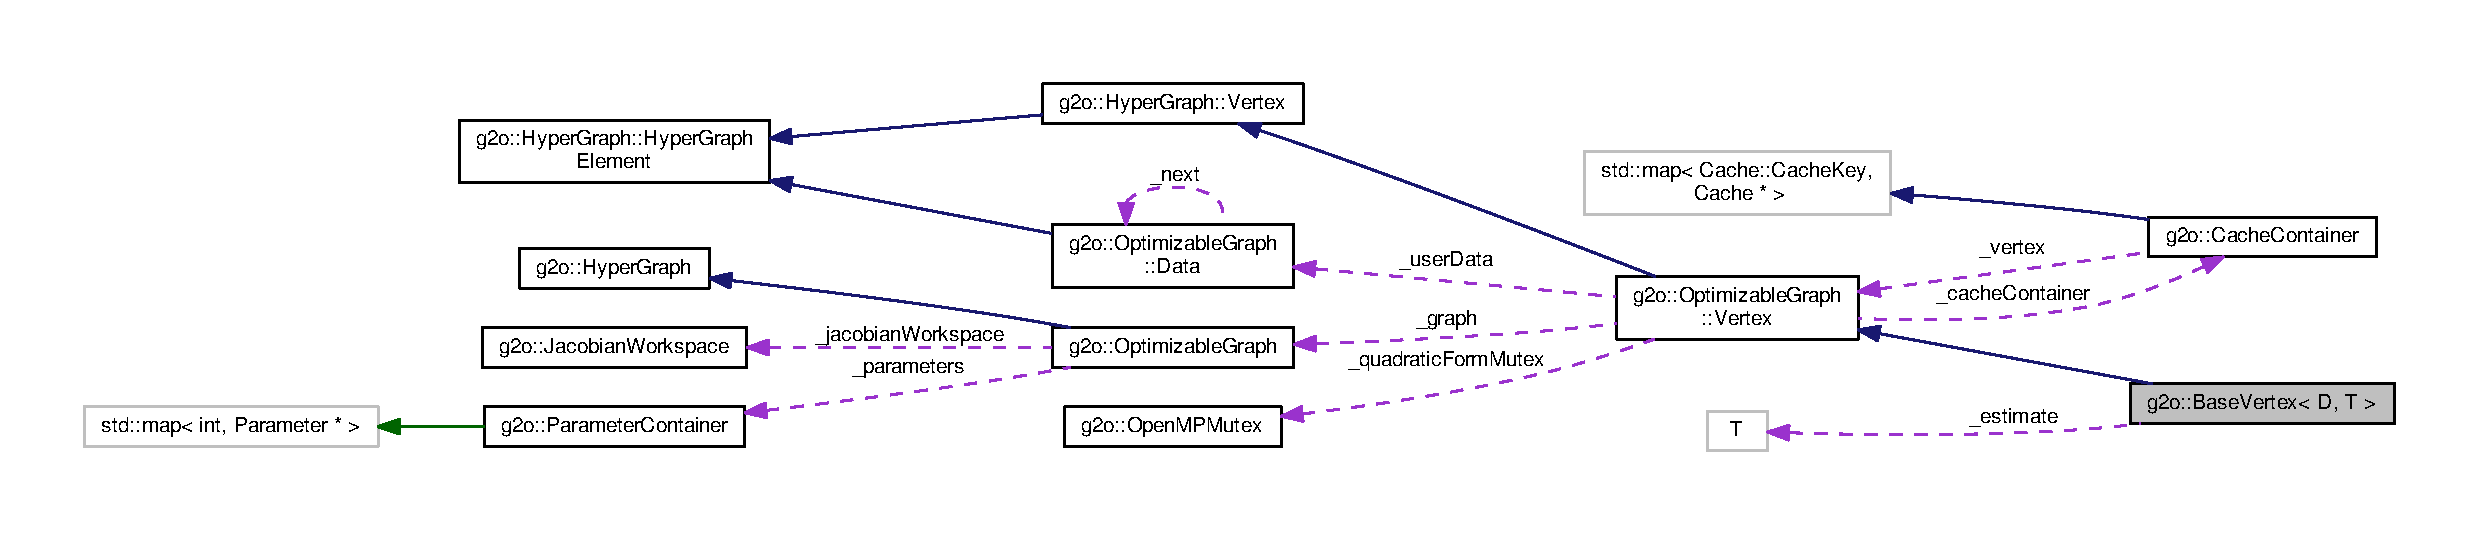
\includegraphics[width=350pt]{classg2o_1_1BaseVertex__coll__graph}
\end{center}
\end{figure}
\subsection*{Public 类型}
\begin{DoxyCompactItemize}
\item 
\hypertarget{classg2o_1_1BaseVertex_aaffb179a0d591da4769ec7c3fc7f7daa}{typedef T {\bfseries Estimate\-Type}}\label{classg2o_1_1BaseVertex_aaffb179a0d591da4769ec7c3fc7f7daa}

\item 
\hypertarget{classg2o_1_1BaseVertex_ae6632291d46b458196bdb021a6c8cba1}{typedef std\-::stack\\*
$<$ Estimate\-Type, std\-::vector\\*
$<$ Estimate\-Type, \\*
Eigen\-::aligned\-\_\-allocator\\*
$<$ Estimate\-Type $>$ $>$ $>$ {\bfseries Backup\-Stack\-Type}}\label{classg2o_1_1BaseVertex_ae6632291d46b458196bdb021a6c8cba1}

\item 
\hypertarget{classg2o_1_1BaseVertex_a887928bc60710e0ec9acb269ee7411db}{typedef Eigen\-::\-Map$<$ Matrix\\*
$<$ double, D, D $>$, Matrix\\*
$<$ double, D, D $>$\-::Flags \\*
\&Aligned\-Bit?Aligned\-:\-Unaligned $>$ {\bfseries Hessian\-Block\-Type}}\label{classg2o_1_1BaseVertex_a887928bc60710e0ec9acb269ee7411db}

\end{DoxyCompactItemize}
\subsection*{Public 成员函数}
\begin{DoxyCompactItemize}
\item 
\hypertarget{classg2o_1_1BaseVertex_ac591409722e675a3b69b9157fb5c7933}{virtual const double \& \hyperlink{classg2o_1_1BaseVertex_ac591409722e675a3b69b9157fb5c7933}{hessian} (int i, int j) const }\label{classg2o_1_1BaseVertex_ac591409722e675a3b69b9157fb5c7933}

\begin{DoxyCompactList}\small\item\em get the element from the hessian matrix \end{DoxyCompactList}\item 
\hypertarget{classg2o_1_1BaseVertex_a6ab2212fdb00dec460299fdbabe09cb9}{virtual double \& {\bfseries hessian} (int i, int j)}\label{classg2o_1_1BaseVertex_a6ab2212fdb00dec460299fdbabe09cb9}

\item 
\hypertarget{classg2o_1_1BaseVertex_a4f302a5d56f733a93fe5e98b49a20a07}{virtual double {\bfseries hessian\-Determinant} () const }\label{classg2o_1_1BaseVertex_a4f302a5d56f733a93fe5e98b49a20a07}

\item 
\hypertarget{classg2o_1_1BaseVertex_aedf92fbb5c2c86185422a955be02a3a6}{virtual double $\ast$ {\bfseries hessian\-Data} ()}\label{classg2o_1_1BaseVertex_aedf92fbb5c2c86185422a955be02a3a6}

\item 
virtual void \hyperlink{classg2o_1_1BaseVertex_a54227ac315e6bc75c63ed117a2c75668}{map\-Hessian\-Memory} (double $\ast$d)
\item 
virtual int \hyperlink{classg2o_1_1BaseVertex_ae9d3f6d4ac4effb78df958df30204c5b}{copy\-B} (double $\ast$b\-\_\-) const 
\item 
\hypertarget{classg2o_1_1BaseVertex_ae50dec87bfcb6a874ba87512c61bada7}{virtual const double \& \hyperlink{classg2o_1_1BaseVertex_ae50dec87bfcb6a874ba87512c61bada7}{b} (int i) const }\label{classg2o_1_1BaseVertex_ae50dec87bfcb6a874ba87512c61bada7}

\begin{DoxyCompactList}\small\item\em get the b vector element \end{DoxyCompactList}\item 
\hypertarget{classg2o_1_1BaseVertex_a5c235369ef3fb58de65b90c8cc37d611}{virtual double \& {\bfseries b} (int i)}\label{classg2o_1_1BaseVertex_a5c235369ef3fb58de65b90c8cc37d611}

\item 
\hypertarget{classg2o_1_1BaseVertex_ac8edea7073e5850c90b0ba37092b8f84}{virtual double $\ast$ \hyperlink{classg2o_1_1BaseVertex_ac8edea7073e5850c90b0ba37092b8f84}{b\-Data} ()}\label{classg2o_1_1BaseVertex_ac8edea7073e5850c90b0ba37092b8f84}

\begin{DoxyCompactList}\small\item\em return a pointer to the b vector associated with this vertex \end{DoxyCompactList}\item 
virtual void \hyperlink{classg2o_1_1BaseVertex_a144f99c7aa36a100dea65b30793e6d76}{clear\-Quadratic\-Form} ()
\item 
virtual double \hyperlink{classg2o_1_1BaseVertex_a0bbd9551b7e03f7e422169e396e8ec9b}{solve\-Direct} (double lambda=0)
\item 
\hypertarget{classg2o_1_1BaseVertex_af7a70ede844ad023ba32edde16c8c745}{Matrix$<$ double, D, 1 $>$ \& \hyperlink{classg2o_1_1BaseVertex_af7a70ede844ad023ba32edde16c8c745}{b} ()}\label{classg2o_1_1BaseVertex_af7a70ede844ad023ba32edde16c8c745}

\begin{DoxyCompactList}\small\item\em return right hand side b of the constructed linear system \end{DoxyCompactList}\item 
\hypertarget{classg2o_1_1BaseVertex_a209c260b9a2730a832270cf3cf7ab605}{const Matrix$<$ double, D, 1 $>$ \& {\bfseries b} () const }\label{classg2o_1_1BaseVertex_a209c260b9a2730a832270cf3cf7ab605}

\item 
\hypertarget{classg2o_1_1BaseVertex_a43bcf2bb3420a0b2cb80bfd297b464a6}{Hessian\-Block\-Type \& \hyperlink{classg2o_1_1BaseVertex_a43bcf2bb3420a0b2cb80bfd297b464a6}{A} ()}\label{classg2o_1_1BaseVertex_a43bcf2bb3420a0b2cb80bfd297b464a6}

\begin{DoxyCompactList}\small\item\em return the hessian block associated with the vertex \end{DoxyCompactList}\item 
\hypertarget{classg2o_1_1BaseVertex_a2f5a9a5bdf0faa43b6082dc3e5a05d45}{const Hessian\-Block\-Type \& {\bfseries A} () const }\label{classg2o_1_1BaseVertex_a2f5a9a5bdf0faa43b6082dc3e5a05d45}

\item 
\hypertarget{classg2o_1_1BaseVertex_ae6edf93fe07aa27579a9352faa83098c}{virtual void \hyperlink{classg2o_1_1BaseVertex_ae6edf93fe07aa27579a9352faa83098c}{push} ()}\label{classg2o_1_1BaseVertex_ae6edf93fe07aa27579a9352faa83098c}

\begin{DoxyCompactList}\small\item\em backup the position of the vertex to a stack \end{DoxyCompactList}\item 
\hypertarget{classg2o_1_1BaseVertex_a502bf3db2ee32061a2c8257ef81a1552}{virtual void \hyperlink{classg2o_1_1BaseVertex_a502bf3db2ee32061a2c8257ef81a1552}{pop} ()}\label{classg2o_1_1BaseVertex_a502bf3db2ee32061a2c8257ef81a1552}

\begin{DoxyCompactList}\small\item\em restore the position of the vertex by retrieving the position from the stack \end{DoxyCompactList}\item 
\hypertarget{classg2o_1_1BaseVertex_a71729c4d91044bde9bfea4c859b0c02d}{virtual void \hyperlink{classg2o_1_1BaseVertex_a71729c4d91044bde9bfea4c859b0c02d}{discard\-Top} ()}\label{classg2o_1_1BaseVertex_a71729c4d91044bde9bfea4c859b0c02d}

\begin{DoxyCompactList}\small\item\em pop the last element from the stack, without restoring the current estimate \end{DoxyCompactList}\item 
\hypertarget{classg2o_1_1BaseVertex_ad40208e3c8e3c221560c69af176b2eb6}{virtual int \hyperlink{classg2o_1_1BaseVertex_ad40208e3c8e3c221560c69af176b2eb6}{stack\-Size} () const }\label{classg2o_1_1BaseVertex_ad40208e3c8e3c221560c69af176b2eb6}

\begin{DoxyCompactList}\small\item\em return the stack size \end{DoxyCompactList}\item 
\hypertarget{classg2o_1_1BaseVertex_abb9caa0d2d00af70e95963a11ee9660a}{const Estimate\-Type \& \hyperlink{classg2o_1_1BaseVertex_abb9caa0d2d00af70e95963a11ee9660a}{estimate} () const }\label{classg2o_1_1BaseVertex_abb9caa0d2d00af70e95963a11ee9660a}

\begin{DoxyCompactList}\small\item\em return the current estimate of the vertex \end{DoxyCompactList}\item 
\hypertarget{classg2o_1_1BaseVertex_acb6e8e8f39caa04f62dd93a3dd400e06}{void \hyperlink{classg2o_1_1BaseVertex_acb6e8e8f39caa04f62dd93a3dd400e06}{set\-Estimate} (const Estimate\-Type \&et)}\label{classg2o_1_1BaseVertex_acb6e8e8f39caa04f62dd93a3dd400e06}

\begin{DoxyCompactList}\small\item\em set the estimate for the vertex also calls update\-Cache() \end{DoxyCompactList}\end{DoxyCompactItemize}
\subsection*{静态 Public 属性}
\begin{DoxyCompactItemize}
\item 
\hypertarget{classg2o_1_1BaseVertex_a9a831bfdf84cfe625d8f942bc4f1c2d1}{static const int \hyperlink{classg2o_1_1BaseVertex_a9a831bfdf84cfe625d8f942bc4f1c2d1}{Dimension} = D}\label{classg2o_1_1BaseVertex_a9a831bfdf84cfe625d8f942bc4f1c2d1}

\begin{DoxyCompactList}\small\item\em dimension of the estimate (minimal) in the manifold space \end{DoxyCompactList}\end{DoxyCompactItemize}
\subsection*{Protected 属性}
\begin{DoxyCompactItemize}
\item 
\hypertarget{classg2o_1_1BaseVertex_afaf73b0e874db76655d90bdb2f156c00}{Hessian\-Block\-Type {\bfseries \-\_\-hessian}}\label{classg2o_1_1BaseVertex_afaf73b0e874db76655d90bdb2f156c00}

\item 
\hypertarget{classg2o_1_1BaseVertex_a70c672f2997275927efa49c1f5b18ac3}{Matrix$<$ double, D, 1 $>$ {\bfseries \-\_\-b}}\label{classg2o_1_1BaseVertex_a70c672f2997275927efa49c1f5b18ac3}

\item 
\hypertarget{classg2o_1_1BaseVertex_ab188c92c3e906c6e06507ae624c0e7ac}{Estimate\-Type {\bfseries \-\_\-estimate}}\label{classg2o_1_1BaseVertex_ab188c92c3e906c6e06507ae624c0e7ac}

\item 
\hypertarget{classg2o_1_1BaseVertex_a936082916993857a77c8318bc3e59d23}{Backup\-Stack\-Type {\bfseries \-\_\-backup}}\label{classg2o_1_1BaseVertex_a936082916993857a77c8318bc3e59d23}

\end{DoxyCompactItemize}
\subsection*{额外继承的成员函数}


\subsection{详细描述}
\subsubsection*{template$<$int D, typename T$>$class g2o\-::\-Base\-Vertex$<$ D, T $>$}

Templatized \hyperlink{classg2o_1_1BaseVertex}{Base\-Vertex}. 

Templatized \hyperlink{classg2o_1_1BaseVertex}{Base\-Vertex} D \-: minimal dimension of the vertex, e.\-g., 3 for rotation in 3\-D T \-: internal type to represent the estimate, e.\-g., Quaternion for rotation in 3\-D 

在文件 base\-\_\-vertex.\-h 第 53 行定义.



\subsection{成员函数说明}
\hypertarget{classg2o_1_1BaseVertex_a144f99c7aa36a100dea65b30793e6d76}{\index{g2o\-::\-Base\-Vertex@{g2o\-::\-Base\-Vertex}!clear\-Quadratic\-Form@{clear\-Quadratic\-Form}}
\index{clear\-Quadratic\-Form@{clear\-Quadratic\-Form}!g2o::BaseVertex@{g2o\-::\-Base\-Vertex}}
\subsubsection[{clear\-Quadratic\-Form}]{\setlength{\rightskip}{0pt plus 5cm}template$<$int D, typename T $>$ void Base\-Vertex\-::clear\-Quadratic\-Form (
\begin{DoxyParamCaption}
{}
\end{DoxyParamCaption}
)\hspace{0.3cm}{\ttfamily [virtual]}}}\label{classg2o_1_1BaseVertex_a144f99c7aa36a100dea65b30793e6d76}
set the b vector part of this vertex to zero 

实现了 \hyperlink{classg2o_1_1OptimizableGraph_1_1Vertex_a803897f6bae25dece4d7e23330f0f9da}{g2o\-::\-Optimizable\-Graph\-::\-Vertex}.



在文件 base\-\_\-vertex.\-h 第 48 行定义.

\hypertarget{classg2o_1_1BaseVertex_ae9d3f6d4ac4effb78df958df30204c5b}{\index{g2o\-::\-Base\-Vertex@{g2o\-::\-Base\-Vertex}!copy\-B@{copy\-B}}
\index{copy\-B@{copy\-B}!g2o::BaseVertex@{g2o\-::\-Base\-Vertex}}
\subsubsection[{copy\-B}]{\setlength{\rightskip}{0pt plus 5cm}template$<$int D, typename T$>$ virtual int {\bf g2o\-::\-Base\-Vertex}$<$ D, T $>$\-::copy\-B (
\begin{DoxyParamCaption}
\item[{double $\ast$}]{b\-\_\-}
\end{DoxyParamCaption}
) const\hspace{0.3cm}{\ttfamily [inline]}, {\ttfamily [virtual]}}}\label{classg2o_1_1BaseVertex_ae9d3f6d4ac4effb78df958df30204c5b}
copies the b vector in the array b\-\_\- \begin{DoxyReturn}{返回}
the number of elements copied 
\end{DoxyReturn}


实现了 \hyperlink{classg2o_1_1OptimizableGraph_1_1Vertex_af544f0050ea6e05950fd6e53931bdf61}{g2o\-::\-Optimizable\-Graph\-::\-Vertex}.



在文件 base\-\_\-vertex.\-h 第 74 行定义.

\hypertarget{classg2o_1_1BaseVertex_a54227ac315e6bc75c63ed117a2c75668}{\index{g2o\-::\-Base\-Vertex@{g2o\-::\-Base\-Vertex}!map\-Hessian\-Memory@{map\-Hessian\-Memory}}
\index{map\-Hessian\-Memory@{map\-Hessian\-Memory}!g2o::BaseVertex@{g2o\-::\-Base\-Vertex}}
\subsubsection[{map\-Hessian\-Memory}]{\setlength{\rightskip}{0pt plus 5cm}template$<$int D, typename T $>$ void Base\-Vertex\-::map\-Hessian\-Memory (
\begin{DoxyParamCaption}
\item[{double $\ast$}]{d}
\end{DoxyParamCaption}
)\hspace{0.3cm}{\ttfamily [virtual]}}}\label{classg2o_1_1BaseVertex_a54227ac315e6bc75c63ed117a2c75668}
maps the internal matrix to some external memory location 

实现了 \hyperlink{classg2o_1_1OptimizableGraph_1_1Vertex_a1008c0f7981a9fb11be3e3df5c4a9758}{g2o\-::\-Optimizable\-Graph\-::\-Vertex}.



在文件 base\-\_\-vertex.\-h 第 53 行定义.

\hypertarget{classg2o_1_1BaseVertex_a0bbd9551b7e03f7e422169e396e8ec9b}{\index{g2o\-::\-Base\-Vertex@{g2o\-::\-Base\-Vertex}!solve\-Direct@{solve\-Direct}}
\index{solve\-Direct@{solve\-Direct}!g2o::BaseVertex@{g2o\-::\-Base\-Vertex}}
\subsubsection[{solve\-Direct}]{\setlength{\rightskip}{0pt plus 5cm}template$<$int D, typename T $>$ double Base\-Vertex\-::solve\-Direct (
\begin{DoxyParamCaption}
\item[{double}]{lambda = {\ttfamily 0}}
\end{DoxyParamCaption}
)\hspace{0.3cm}{\ttfamily [virtual]}}}\label{classg2o_1_1BaseVertex_a0bbd9551b7e03f7e422169e396e8ec9b}
updates the current vertex with the direct solution x += H\-\_\-ii \begin{DoxyReturn}{返回}
the determinant of the inverted hessian 
\end{DoxyReturn}


实现了 \hyperlink{classg2o_1_1OptimizableGraph_1_1Vertex_a61c4e7b7a7a61e1f287069a8cb01004f}{g2o\-::\-Optimizable\-Graph\-::\-Vertex}.



在文件 base\-\_\-vertex.\-h 第 37 行定义.



该类的文档由以下文件生成\-:\begin{DoxyCompactItemize}
\item 
Thirdparty/g2o/g2o/core/base\-\_\-vertex.\-h\item 
Thirdparty/g2o/g2o/core/base\-\_\-vertex.\-hpp\end{DoxyCompactItemize}

\hypertarget{classg2o_1_1BlockSolver}{\section{g2o\-:\-:Block\-Solver$<$ Traits $>$ 模板类 参考}
\label{classg2o_1_1BlockSolver}\index{g2o\-::\-Block\-Solver$<$ Traits $>$@{g2o\-::\-Block\-Solver$<$ Traits $>$}}
}


Implementation of a solver operating on the blocks of the Hessian.  




{\ttfamily \#include $<$block\-\_\-solver.\-h$>$}



类 g2o\-:\-:Block\-Solver$<$ Traits $>$ 继承关系图\-:
\nopagebreak
\begin{figure}[H]
\begin{center}
\leavevmode
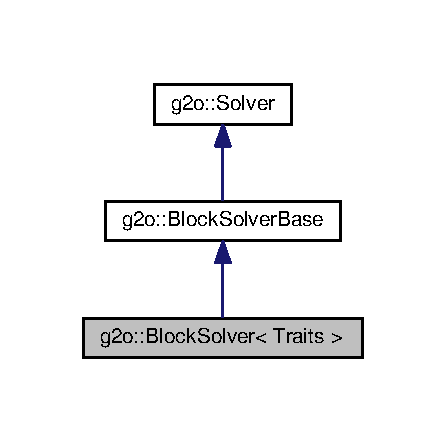
\includegraphics[width=214pt]{classg2o_1_1BlockSolver__inherit__graph}
\end{center}
\end{figure}


g2o\-:\-:Block\-Solver$<$ Traits $>$ 的协作图\-:
\nopagebreak
\begin{figure}[H]
\begin{center}
\leavevmode
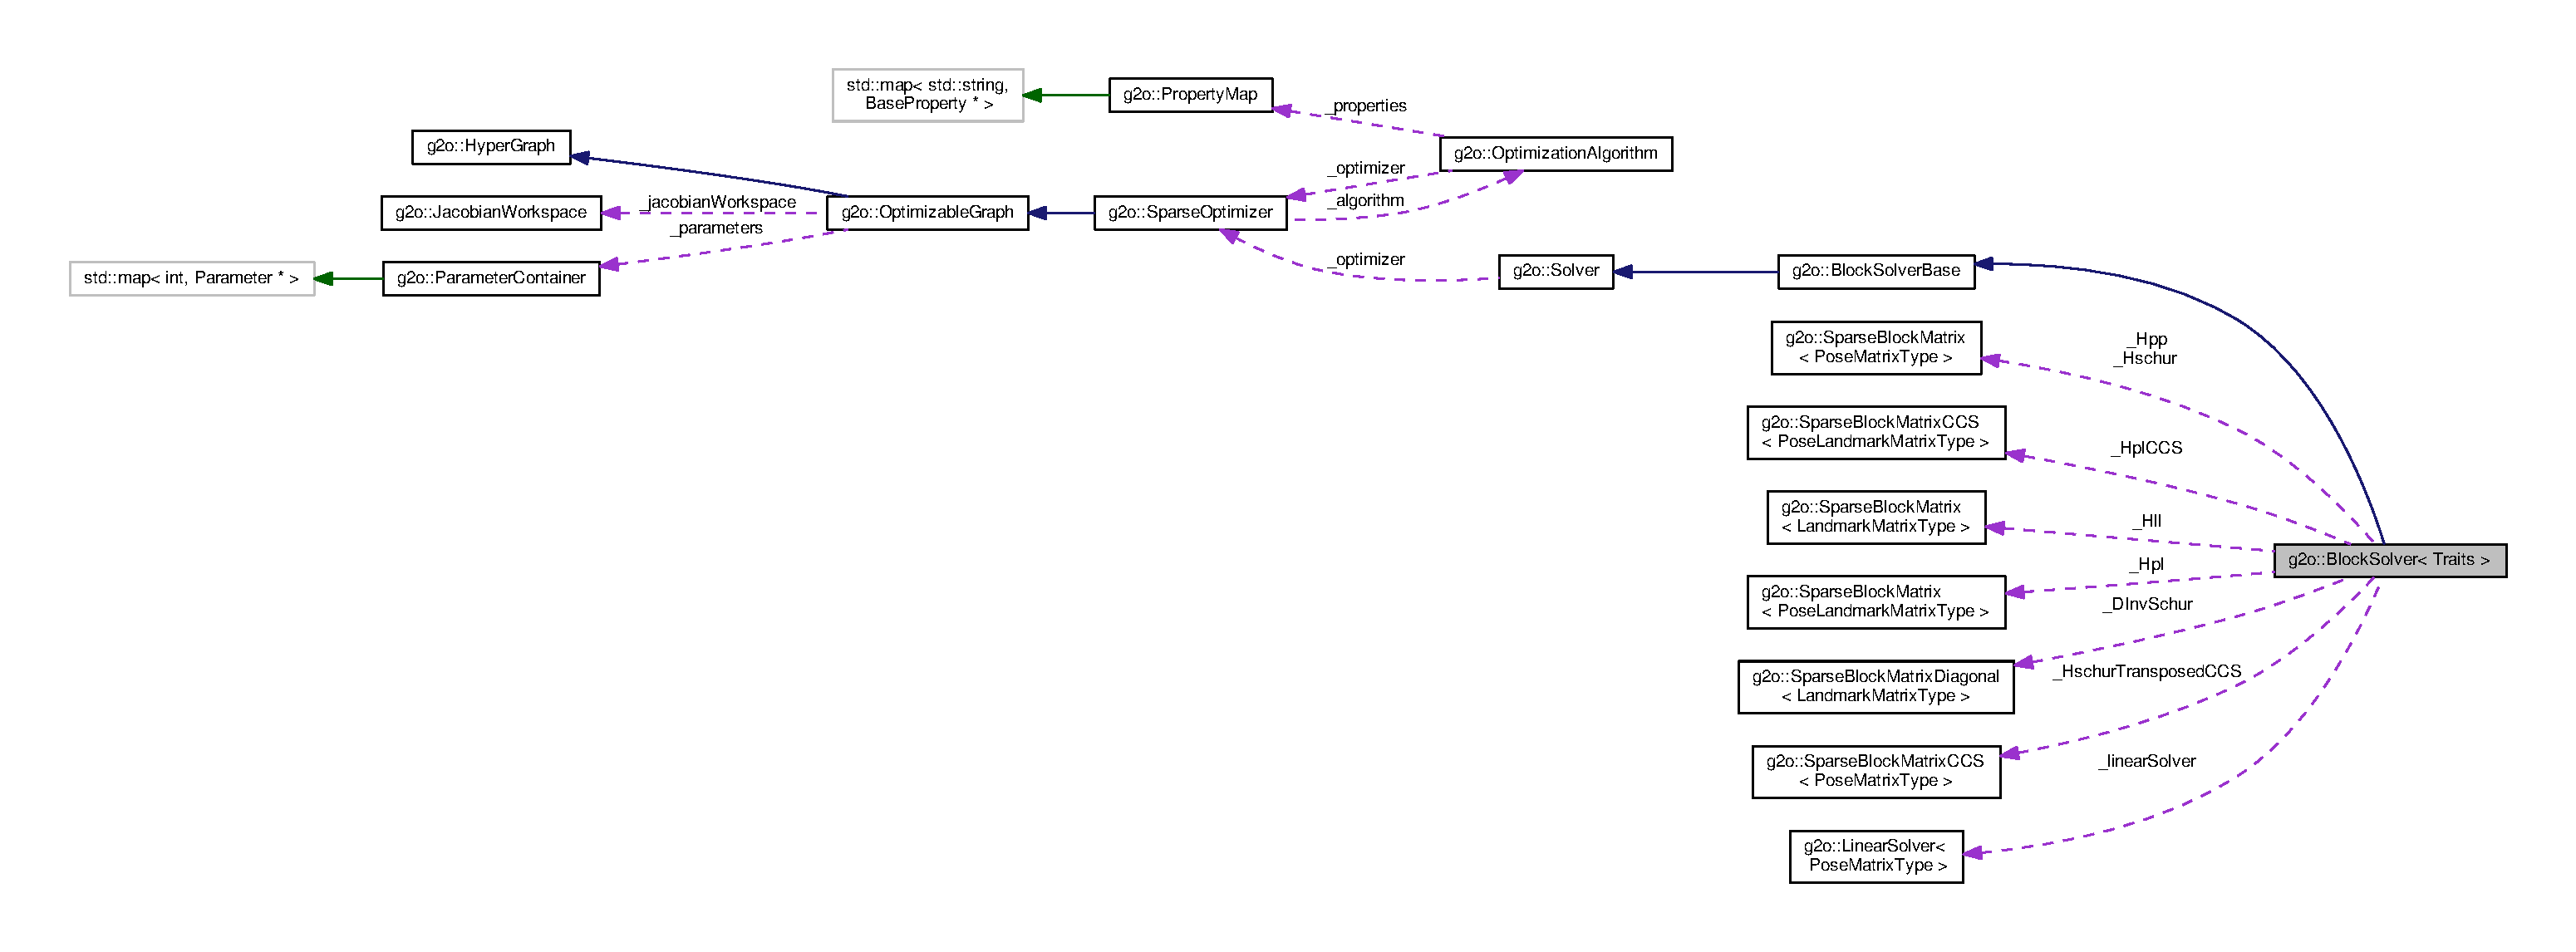
\includegraphics[width=350pt]{classg2o_1_1BlockSolver__coll__graph}
\end{center}
\end{figure}
\subsection*{Public 类型}
\begin{DoxyCompactItemize}
\item 
\hypertarget{classg2o_1_1BlockSolver_a8c7c43d361bd31e3e0353889ba703bc0}{typedef Traits\-::\-Pose\-Matrix\-Type {\bfseries Pose\-Matrix\-Type}}\label{classg2o_1_1BlockSolver_a8c7c43d361bd31e3e0353889ba703bc0}

\item 
\hypertarget{classg2o_1_1BlockSolver_afd898a666343291129d37a979e23ded6}{typedef Traits\-::\-Landmark\-Matrix\-Type {\bfseries Landmark\-Matrix\-Type}}\label{classg2o_1_1BlockSolver_afd898a666343291129d37a979e23ded6}

\item 
\hypertarget{classg2o_1_1BlockSolver_a96bf60b923f816086cd2f24de38736ec}{typedef \\*
Traits\-::\-Pose\-Landmark\-Matrix\-Type {\bfseries Pose\-Landmark\-Matrix\-Type}}\label{classg2o_1_1BlockSolver_a96bf60b923f816086cd2f24de38736ec}

\item 
\hypertarget{classg2o_1_1BlockSolver_a65d51b9281e2e2597df05eb00801ee76}{typedef Traits\-::\-Pose\-Vector\-Type {\bfseries Pose\-Vector\-Type}}\label{classg2o_1_1BlockSolver_a65d51b9281e2e2597df05eb00801ee76}

\item 
\hypertarget{classg2o_1_1BlockSolver_a19ade5e432f32e46557192ae75074304}{typedef Traits\-::\-Landmark\-Vector\-Type {\bfseries Landmark\-Vector\-Type}}\label{classg2o_1_1BlockSolver_a19ade5e432f32e46557192ae75074304}

\item 
\hypertarget{classg2o_1_1BlockSolver_a0e7f862860a1e3391cec3cfaf69c48be}{typedef Traits\-::\-Pose\-Hessian\-Type {\bfseries Pose\-Hessian\-Type}}\label{classg2o_1_1BlockSolver_a0e7f862860a1e3391cec3cfaf69c48be}

\item 
\hypertarget{classg2o_1_1BlockSolver_a465b1252905d90fd69b4243716620c45}{typedef Traits\-::\-Landmark\-Hessian\-Type {\bfseries Landmark\-Hessian\-Type}}\label{classg2o_1_1BlockSolver_a465b1252905d90fd69b4243716620c45}

\item 
\hypertarget{classg2o_1_1BlockSolver_aed8b44e394d2f19ca03c87adf90cc97c}{typedef \\*
Traits\-::\-Pose\-Landmark\-Hessian\-Type {\bfseries Pose\-Landmark\-Hessian\-Type}}\label{classg2o_1_1BlockSolver_aed8b44e394d2f19ca03c87adf90cc97c}

\item 
\hypertarget{classg2o_1_1BlockSolver_a717fa8cb1dd5a212e41d8ebef67955e6}{typedef Traits\-::\-Linear\-Solver\-Type {\bfseries Linear\-Solver\-Type}}\label{classg2o_1_1BlockSolver_a717fa8cb1dd5a212e41d8ebef67955e6}

\end{DoxyCompactItemize}
\subsection*{Public 成员函数}
\begin{DoxyCompactItemize}
\item 
\hyperlink{classg2o_1_1BlockSolver_a04701a223a14708c9c84ce4d7e7af3f6}{Block\-Solver} (Linear\-Solver\-Type $\ast$linear\-Solver)
\item 
virtual bool \hyperlink{classg2o_1_1BlockSolver_a8bf01018abc3bfddfa3b29a380a1d6cb}{init} (\hyperlink{classg2o_1_1SparseOptimizer}{Sparse\-Optimizer} $\ast$optmizer, bool online=false)
\item 
virtual bool \hyperlink{classg2o_1_1BlockSolver_a17e4392d3cca9a9d7cf38bb46d073b86}{build\-Structure} (bool zero\-Blocks=false)
\item 
virtual bool \hyperlink{classg2o_1_1BlockSolver_acc497239c5e681ddec2140e34dfc5938}{update\-Structure} (const std\-::vector$<$ \hyperlink{classg2o_1_1HyperGraph_1_1Vertex}{Hyper\-Graph\-::\-Vertex} $\ast$ $>$ \&vset, const Hyper\-Graph\-::\-Edge\-Set \&edges)
\item 
virtual bool \hyperlink{classg2o_1_1BlockSolver_a2654a8d52f38e5ce23720a8de302e2e7}{build\-System} ()
\item 
virtual bool \hyperlink{classg2o_1_1BlockSolver_a589a75a131cce100c1945ad2786214d7}{solve} ()
\item 
virtual bool \hyperlink{classg2o_1_1BlockSolver_ac21cd7e2c9b8a1414f7a2dccb0d30a0e}{compute\-Marginals} (\hyperlink{classg2o_1_1SparseBlockMatrix}{Sparse\-Block\-Matrix}$<$ Matrix\-Xd $>$ \&spinv, const std\-::vector$<$ std\-::pair$<$ int, int $>$ $>$ \&block\-Indices)
\item 
virtual bool \hyperlink{classg2o_1_1BlockSolver_acc63a23e5b35e4f72d46dc22719aa56f}{set\-Lambda} (double lambda, bool backup=false)
\item 
virtual void \hyperlink{classg2o_1_1BlockSolver_a2136931d7aa2f54df5207556c4685809}{restore\-Diagonal} ()
\item 
virtual bool \hyperlink{classg2o_1_1BlockSolver_a68dc822ce48e80ceacce69c7bd029674}{supports\-Schur} ()
\item 
\hypertarget{classg2o_1_1BlockSolver_a382173946f1dd929a625e3708c959883}{virtual bool \hyperlink{classg2o_1_1BlockSolver_a382173946f1dd929a625e3708c959883}{schur} ()}\label{classg2o_1_1BlockSolver_a382173946f1dd929a625e3708c959883}

\begin{DoxyCompactList}\small\item\em should the solver perform the schur complement or not \end{DoxyCompactList}\item 
\hypertarget{classg2o_1_1BlockSolver_a6dd8e7e7a099410005cb96ff874d8866}{virtual void {\bfseries set\-Schur} (bool s)}\label{classg2o_1_1BlockSolver_a6dd8e7e7a099410005cb96ff874d8866}

\item 
\hypertarget{classg2o_1_1BlockSolver_adb09637f5f87327d26928f672d6caadf}{\hyperlink{classg2o_1_1LinearSolver}{Linear\-Solver}$<$ Pose\-Matrix\-Type $>$ $\ast$ {\bfseries linear\-Solver} () const }\label{classg2o_1_1BlockSolver_adb09637f5f87327d26928f672d6caadf}

\item 
virtual void \hyperlink{classg2o_1_1BlockSolver_a1bff5dc13e3408fa76c019347104acd0}{set\-Write\-Debug} (bool write\-Debug)
\item 
\hypertarget{classg2o_1_1BlockSolver_a5a127b36e9f6ec45b2b1d39c22a9901f}{virtual bool {\bfseries write\-Debug} () const }\label{classg2o_1_1BlockSolver_a5a127b36e9f6ec45b2b1d39c22a9901f}

\item 
\hypertarget{classg2o_1_1BlockSolver_a79adbc8926b11c564bdd8cf73a55b1ef}{virtual bool \hyperlink{classg2o_1_1BlockSolver_a79adbc8926b11c564bdd8cf73a55b1ef}{save\-Hessian} (const std\-::string \&file\-Name) const }\label{classg2o_1_1BlockSolver_a79adbc8926b11c564bdd8cf73a55b1ef}

\begin{DoxyCompactList}\small\item\em write the hessian to disk using the specified file name \end{DoxyCompactList}\item 
virtual void \hyperlink{classg2o_1_1BlockSolver_a615892075357273ec8bb06e101d9155b}{multiply\-Hessian} (double $\ast$dest, const double $\ast$src) const 
\end{DoxyCompactItemize}
\subsection*{静态 Public 属性}
\begin{DoxyCompactItemize}
\item 
\hypertarget{classg2o_1_1BlockSolver_a9a68f557c8e04cd76565fc45e1747e45}{static const int {\bfseries Pose\-Dim} = Traits\-::\-Pose\-Dim}\label{classg2o_1_1BlockSolver_a9a68f557c8e04cd76565fc45e1747e45}

\item 
\hypertarget{classg2o_1_1BlockSolver_a2d5e499f65a71985a8256e98c1608dd9}{static const int {\bfseries Landmark\-Dim} = Traits\-::\-Landmark\-Dim}\label{classg2o_1_1BlockSolver_a2d5e499f65a71985a8256e98c1608dd9}

\end{DoxyCompactItemize}
\subsection*{Protected 成员函数}
\begin{DoxyCompactItemize}
\item 
\hypertarget{classg2o_1_1BlockSolver_a0075af2df18364cf99fd80f813b8ce4b}{void {\bfseries resize} (int $\ast$block\-Pose\-Indices, int num\-Pose\-Blocks, int $\ast$block\-Landmark\-Indices, int num\-Landmark\-Blocks, int total\-Dim)}\label{classg2o_1_1BlockSolver_a0075af2df18364cf99fd80f813b8ce4b}

\item 
\hypertarget{classg2o_1_1BlockSolver_a1877467844b7b9ab51bd6600e3a93eb0}{void {\bfseries deallocate} ()}\label{classg2o_1_1BlockSolver_a1877467844b7b9ab51bd6600e3a93eb0}

\end{DoxyCompactItemize}
\subsection*{Protected 属性}
\begin{DoxyCompactItemize}
\item 
\hypertarget{classg2o_1_1BlockSolver_ac222d4342825ed8632a87b4f5be94618}{\hyperlink{classg2o_1_1SparseBlockMatrix}{Sparse\-Block\-Matrix}\\*
$<$ Pose\-Matrix\-Type $>$ $\ast$ {\bfseries \-\_\-\-Hpp}}\label{classg2o_1_1BlockSolver_ac222d4342825ed8632a87b4f5be94618}

\item 
\hypertarget{classg2o_1_1BlockSolver_a88d4c24df24a8fb72be1a4e4cff03d71}{\hyperlink{classg2o_1_1SparseBlockMatrix}{Sparse\-Block\-Matrix}\\*
$<$ Landmark\-Matrix\-Type $>$ $\ast$ {\bfseries \-\_\-\-Hll}}\label{classg2o_1_1BlockSolver_a88d4c24df24a8fb72be1a4e4cff03d71}

\item 
\hypertarget{classg2o_1_1BlockSolver_a0f6051339990e95aa587145a8a6f4f5f}{\hyperlink{classg2o_1_1SparseBlockMatrix}{Sparse\-Block\-Matrix}\\*
$<$ Pose\-Landmark\-Matrix\-Type $>$ $\ast$ {\bfseries \-\_\-\-Hpl}}\label{classg2o_1_1BlockSolver_a0f6051339990e95aa587145a8a6f4f5f}

\item 
\hypertarget{classg2o_1_1BlockSolver_a46977934a3e4fb0cd36bc4181ed3ec0e}{\hyperlink{classg2o_1_1SparseBlockMatrix}{Sparse\-Block\-Matrix}\\*
$<$ Pose\-Matrix\-Type $>$ $\ast$ {\bfseries \-\_\-\-Hschur}}\label{classg2o_1_1BlockSolver_a46977934a3e4fb0cd36bc4181ed3ec0e}

\item 
\hypertarget{classg2o_1_1BlockSolver_ad6a1a8f17c8fb854962a8204c79bc981}{\hyperlink{classg2o_1_1SparseBlockMatrixDiagonal}{Sparse\-Block\-Matrix\-Diagonal}\\*
$<$ Landmark\-Matrix\-Type $>$ $\ast$ {\bfseries \-\_\-\-D\-Inv\-Schur}}\label{classg2o_1_1BlockSolver_ad6a1a8f17c8fb854962a8204c79bc981}

\item 
\hypertarget{classg2o_1_1BlockSolver_ab54eb7bb13f8b3a8a5f135a98f2050ec}{\hyperlink{classg2o_1_1SparseBlockMatrixCCS}{Sparse\-Block\-Matrix\-C\-C\-S}\\*
$<$ Pose\-Landmark\-Matrix\-Type $>$ $\ast$ {\bfseries \-\_\-\-Hpl\-C\-C\-S}}\label{classg2o_1_1BlockSolver_ab54eb7bb13f8b3a8a5f135a98f2050ec}

\item 
\hypertarget{classg2o_1_1BlockSolver_acea4b8ea8db5a29b63bea4bc568b0b26}{\hyperlink{classg2o_1_1SparseBlockMatrixCCS}{Sparse\-Block\-Matrix\-C\-C\-S}\\*
$<$ Pose\-Matrix\-Type $>$ $\ast$ {\bfseries \-\_\-\-Hschur\-Transposed\-C\-C\-S}}\label{classg2o_1_1BlockSolver_acea4b8ea8db5a29b63bea4bc568b0b26}

\item 
\hypertarget{classg2o_1_1BlockSolver_a676a4ef473ccaecb23050284e19659af}{\hyperlink{classg2o_1_1LinearSolver}{Linear\-Solver}$<$ Pose\-Matrix\-Type $>$ $\ast$ {\bfseries \-\_\-linear\-Solver}}\label{classg2o_1_1BlockSolver_a676a4ef473ccaecb23050284e19659af}

\item 
\hypertarget{classg2o_1_1BlockSolver_a3cb6f86c522c2ea26478ad44b7c32f76}{std\-::vector$<$ Pose\-Vector\-Type, \\*
Eigen\-::aligned\-\_\-allocator\\*
$<$ Pose\-Vector\-Type $>$ $>$ {\bfseries \-\_\-diagonal\-Backup\-Pose}}\label{classg2o_1_1BlockSolver_a3cb6f86c522c2ea26478ad44b7c32f76}

\item 
\hypertarget{classg2o_1_1BlockSolver_a3bc5b19faa2c45e2c04a6743b3a083de}{std\-::vector\\*
$<$ Landmark\-Vector\-Type, \\*
Eigen\-::aligned\-\_\-allocator\\*
$<$ Landmark\-Vector\-Type $>$ $>$ {\bfseries \-\_\-diagonal\-Backup\-Landmark}}\label{classg2o_1_1BlockSolver_a3bc5b19faa2c45e2c04a6743b3a083de}

\item 
\hypertarget{classg2o_1_1BlockSolver_ab375a5fac964182442f38288bd8a103a}{bool {\bfseries \-\_\-do\-Schur}}\label{classg2o_1_1BlockSolver_ab375a5fac964182442f38288bd8a103a}

\item 
\hypertarget{classg2o_1_1BlockSolver_a416f480d4b27d7f8962ae7ae363f2e32}{double $\ast$ {\bfseries \-\_\-coefficients}}\label{classg2o_1_1BlockSolver_a416f480d4b27d7f8962ae7ae363f2e32}

\item 
\hypertarget{classg2o_1_1BlockSolver_aafddeb1d0a4218fc9c3c77169e20f81a}{double $\ast$ {\bfseries \-\_\-bschur}}\label{classg2o_1_1BlockSolver_aafddeb1d0a4218fc9c3c77169e20f81a}

\item 
\hypertarget{classg2o_1_1BlockSolver_a709259fc290d746f4174d25410b7458a}{int {\bfseries \-\_\-num\-Poses}}\label{classg2o_1_1BlockSolver_a709259fc290d746f4174d25410b7458a}

\item 
\hypertarget{classg2o_1_1BlockSolver_ab98231b7ca8e6d7f138c33d26c6f4326}{int {\bfseries \-\_\-num\-Landmarks}}\label{classg2o_1_1BlockSolver_ab98231b7ca8e6d7f138c33d26c6f4326}

\item 
\hypertarget{classg2o_1_1BlockSolver_a39ec000379885ce09cdd8c23ab6d4567}{int {\bfseries \-\_\-size\-Poses}}\label{classg2o_1_1BlockSolver_a39ec000379885ce09cdd8c23ab6d4567}

\item 
\hypertarget{classg2o_1_1BlockSolver_a13a49b5aac8ae3b12ed0c349fc0788e7}{int {\bfseries \-\_\-size\-Landmarks}}\label{classg2o_1_1BlockSolver_a13a49b5aac8ae3b12ed0c349fc0788e7}

\end{DoxyCompactItemize}


\subsection{详细描述}
\subsubsection*{template$<$typename Traits$>$class g2o\-::\-Block\-Solver$<$ Traits $>$}

Implementation of a solver operating on the blocks of the Hessian. 

在文件 block\-\_\-solver.\-h 第 97 行定义.



\subsection{构造及析构函数说明}
\hypertarget{classg2o_1_1BlockSolver_a04701a223a14708c9c84ce4d7e7af3f6}{\index{g2o\-::\-Block\-Solver@{g2o\-::\-Block\-Solver}!Block\-Solver@{Block\-Solver}}
\index{Block\-Solver@{Block\-Solver}!g2o::BlockSolver@{g2o\-::\-Block\-Solver}}
\subsubsection[{Block\-Solver}]{\setlength{\rightskip}{0pt plus 5cm}template$<$typename Traits $>$ {\bf g2o\-::\-Block\-Solver}$<$ Traits $>$\-::{\bf Block\-Solver} (
\begin{DoxyParamCaption}
\item[{Linear\-Solver\-Type $\ast$}]{linear\-Solver}
\end{DoxyParamCaption}
)}}\label{classg2o_1_1BlockSolver_a04701a223a14708c9c84ce4d7e7af3f6}
allocate a block solver ontop of the underlying linear solver. N\-O\-T\-E\-: The \hyperlink{classg2o_1_1BlockSolver}{Block\-Solver} assumes exclusive access to the linear solver and will therefore free the pointer in its destructor. 

在文件 block\-\_\-solver.\-hpp 第 43 行定义.



\subsection{成员函数说明}
\hypertarget{classg2o_1_1BlockSolver_a17e4392d3cca9a9d7cf38bb46d073b86}{\index{g2o\-::\-Block\-Solver@{g2o\-::\-Block\-Solver}!build\-Structure@{build\-Structure}}
\index{build\-Structure@{build\-Structure}!g2o::BlockSolver@{g2o\-::\-Block\-Solver}}
\subsubsection[{build\-Structure}]{\setlength{\rightskip}{0pt plus 5cm}template$<$typename Traits $>$ bool {\bf g2o\-::\-Block\-Solver}$<$ Traits $>$\-::build\-Structure (
\begin{DoxyParamCaption}
\item[{bool}]{zero\-Blocks = {\ttfamily false}}
\end{DoxyParamCaption}
)\hspace{0.3cm}{\ttfamily [virtual]}}}\label{classg2o_1_1BlockSolver_a17e4392d3cca9a9d7cf38bb46d073b86}
build the structure of the system 

实现了 \hyperlink{classg2o_1_1Solver_a6c93ac0f528ffe05867d33150c54f46f}{g2o\-::\-Solver}.



在文件 block\-\_\-solver.\-hpp 第 144 行定义.



参考 g2o\-::\-Sparse\-Block\-Matrix\-Hash\-Map$<$ Matrix\-Type $>$\-::add\-Block(), g2o\-::\-Sparse\-Block\-Matrix\-Hash\-Map$<$ Matrix\-Type $>$\-::block\-Cols(), g2o\-::\-Optimizable\-Graph\-::\-Vertex\-::dimension(), g2o\-::\-Hyper\-Graph\-::\-Vertex\-::edges(), g2o\-::\-Optimizable\-Graph\-::\-Vertex\-::hessian\-Index(), g2o\-::\-Optimizable\-Graph\-::\-Vertex\-::map\-Hessian\-Memory(), g2o\-::\-Optimizable\-Graph\-::\-Edge\-::map\-Hessian\-Memory(), g2o\-::\-Optimizable\-Graph\-::\-Vertex\-::marginalized(), g2o\-::\-Optimizable\-Graph\-::\-Vertex\-::set\-Col\-In\-Hessian(), g2o\-::\-Hyper\-Graph\-::\-Edge\-::vertex() , 以及 g2o\-::\-Hyper\-Graph\-::\-Edge\-::vertices().



函数调用图\-:
\nopagebreak
\begin{figure}[H]
\begin{center}
\leavevmode
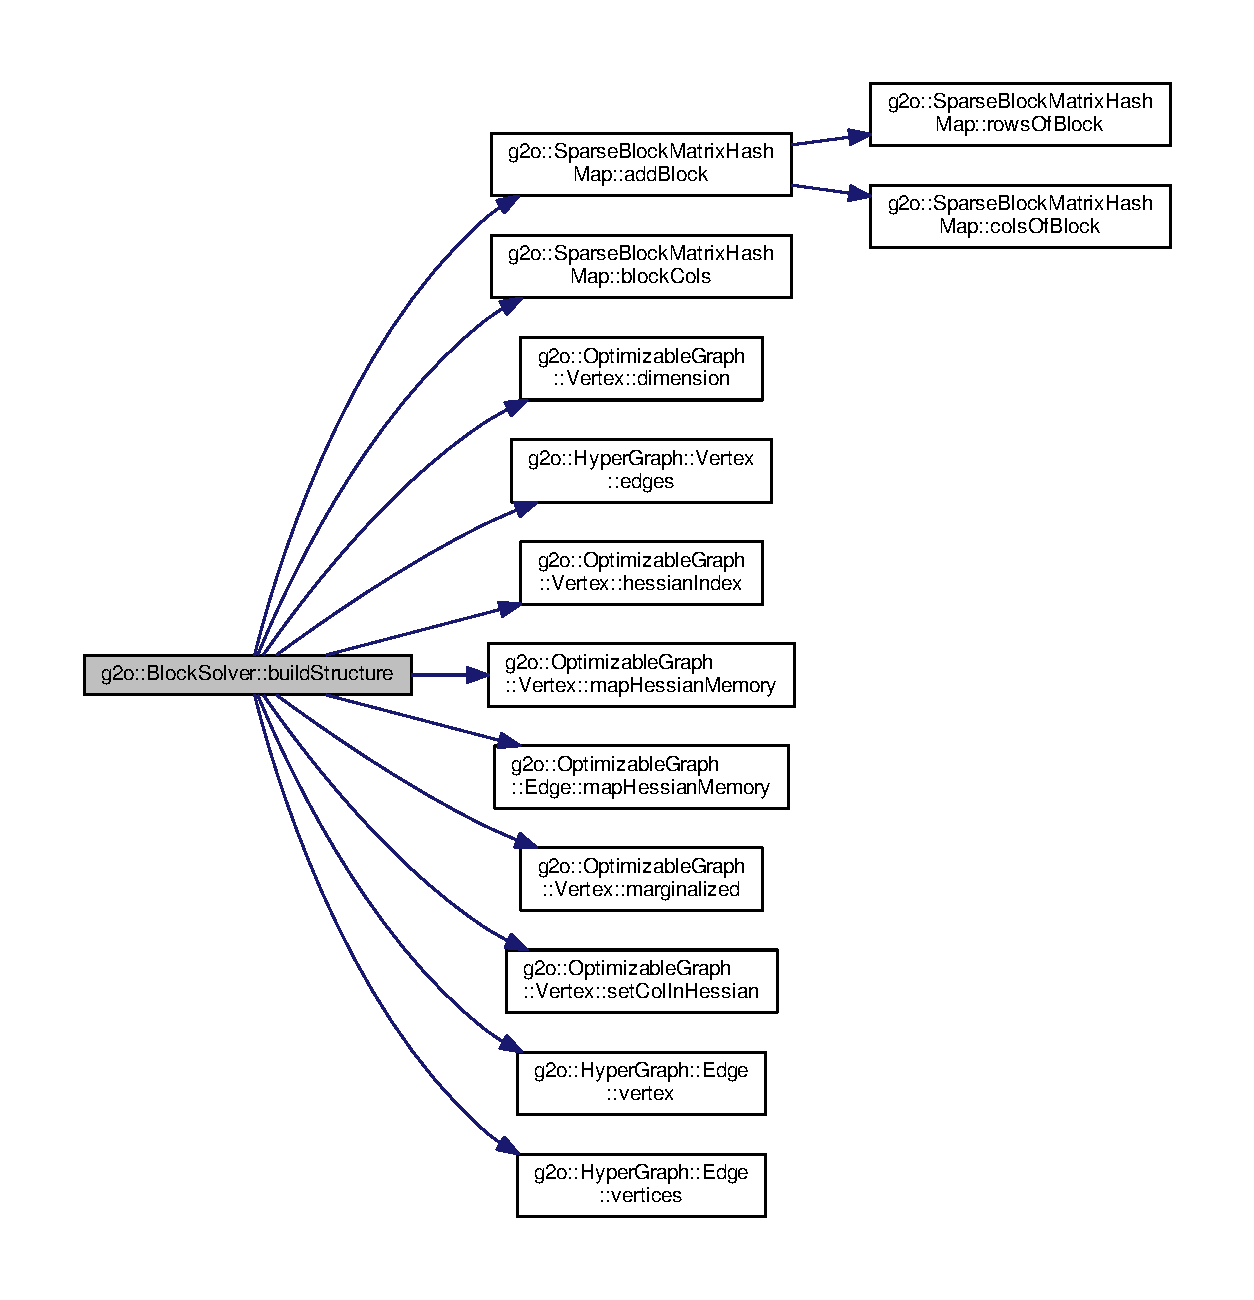
\includegraphics[width=350pt]{classg2o_1_1BlockSolver_a17e4392d3cca9a9d7cf38bb46d073b86_cgraph}
\end{center}
\end{figure}


\hypertarget{classg2o_1_1BlockSolver_a2654a8d52f38e5ce23720a8de302e2e7}{\index{g2o\-::\-Block\-Solver@{g2o\-::\-Block\-Solver}!build\-System@{build\-System}}
\index{build\-System@{build\-System}!g2o::BlockSolver@{g2o\-::\-Block\-Solver}}
\subsubsection[{build\-System}]{\setlength{\rightskip}{0pt plus 5cm}template$<$typename Traits $>$ bool {\bf g2o\-::\-Block\-Solver}$<$ Traits $>$\-::build\-System (
\begin{DoxyParamCaption}
{}
\end{DoxyParamCaption}
)\hspace{0.3cm}{\ttfamily [virtual]}}}\label{classg2o_1_1BlockSolver_a2654a8d52f38e5ce23720a8de302e2e7}
build the current system 

实现了 \hyperlink{classg2o_1_1Solver_ac1565e85d5ca68a87ad7f06f8164a8c0}{g2o\-::\-Solver}.



在文件 block\-\_\-solver.\-hpp 第 503 行定义.



参考 g2o\-::\-Optimizable\-Graph\-::\-Vertex\-::clear\-Quadratic\-Form(), g2o\-::\-Optimizable\-Graph\-::\-Vertex\-::col\-In\-Hessian(), g2o\-::\-Optimizable\-Graph\-::\-Edge\-::construct\-Quadratic\-Form(), g2o\-::\-Optimizable\-Graph\-::\-Vertex\-::copy\-B(), g2o\-::\-Optimizable\-Graph\-::\-Vertex\-::dimension(), g2o\-::\-Optimizable\-Graph\-::\-Edge\-::dimension(), g2o\-::\-Optimizable\-Graph\-::\-Vertex\-::fixed(), g2o\-::\-Optimizable\-Graph\-::\-Edge\-::linearize\-Oplus(), g2o\-::\-Optimizable\-Graph\-::\-Vertex\-::marginalized(), g2o\-::\-Hyper\-Graph\-::\-Edge\-::vertex(), g2o\-::\-Hyper\-Graph\-::\-Edge\-::vertices() , 以及 g2o\-::\-Jacobian\-Workspace\-::workspace\-For\-Vertex().



函数调用图\-:
\nopagebreak
\begin{figure}[H]
\begin{center}
\leavevmode
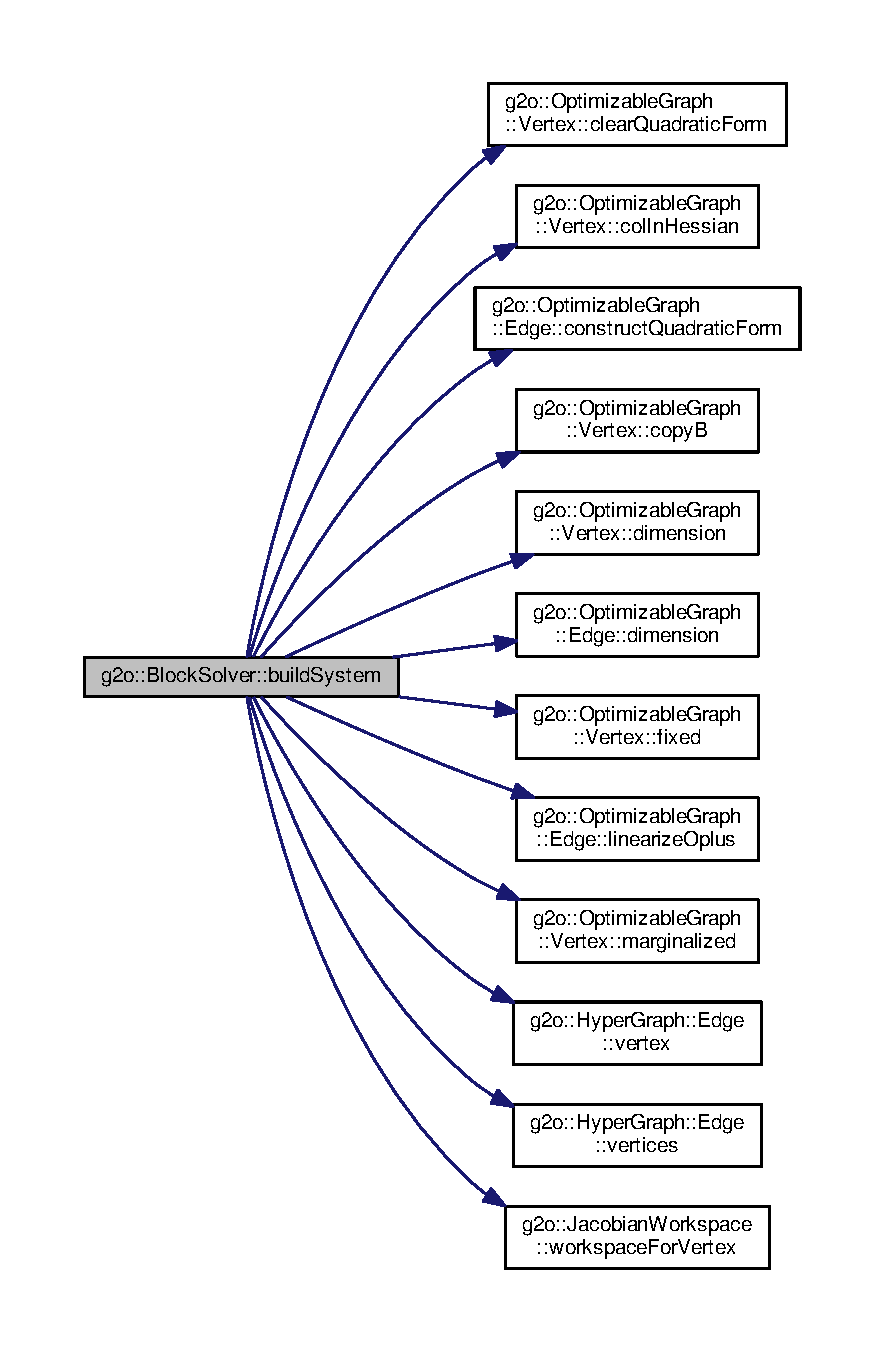
\includegraphics[width=350pt]{classg2o_1_1BlockSolver_a2654a8d52f38e5ce23720a8de302e2e7_cgraph}
\end{center}
\end{figure}


\hypertarget{classg2o_1_1BlockSolver_ac21cd7e2c9b8a1414f7a2dccb0d30a0e}{\index{g2o\-::\-Block\-Solver@{g2o\-::\-Block\-Solver}!compute\-Marginals@{compute\-Marginals}}
\index{compute\-Marginals@{compute\-Marginals}!g2o::BlockSolver@{g2o\-::\-Block\-Solver}}
\subsubsection[{compute\-Marginals}]{\setlength{\rightskip}{0pt plus 5cm}template$<$typename Traits $>$ bool {\bf g2o\-::\-Block\-Solver}$<$ Traits $>$\-::compute\-Marginals (
\begin{DoxyParamCaption}
\item[{{\bf Sparse\-Block\-Matrix}$<$ Matrix\-Xd $>$ \&}]{spinv, }
\item[{const std\-::vector$<$ std\-::pair$<$ int, int $>$ $>$ \&}]{block\-Indices}
\end{DoxyParamCaption}
)\hspace{0.3cm}{\ttfamily [virtual]}}}\label{classg2o_1_1BlockSolver_ac21cd7e2c9b8a1414f7a2dccb0d30a0e}
computes the block diagonal elements of the pattern specified in the input and stores them in given \hyperlink{classg2o_1_1SparseBlockMatrix}{Sparse\-Block\-Matrix} 

实现了 \hyperlink{classg2o_1_1Solver_afc33768e6c024e11d9e3c9d938b59b7f}{g2o\-::\-Solver}.



在文件 block\-\_\-solver.\-hpp 第 491 行定义.



参考 g2o\-::\-G2\-O\-Batch\-Statistics\-::time\-Marginals.

\hypertarget{classg2o_1_1BlockSolver_a8bf01018abc3bfddfa3b29a380a1d6cb}{\index{g2o\-::\-Block\-Solver@{g2o\-::\-Block\-Solver}!init@{init}}
\index{init@{init}!g2o::BlockSolver@{g2o\-::\-Block\-Solver}}
\subsubsection[{init}]{\setlength{\rightskip}{0pt plus 5cm}template$<$typename Traits $>$ bool {\bf g2o\-::\-Block\-Solver}$<$ Traits $>$\-::init (
\begin{DoxyParamCaption}
\item[{{\bf Sparse\-Optimizer} $\ast$}]{optimizer, }
\item[{bool}]{online = {\ttfamily false}}
\end{DoxyParamCaption}
)\hspace{0.3cm}{\ttfamily [virtual]}}}\label{classg2o_1_1BlockSolver_a8bf01018abc3bfddfa3b29a380a1d6cb}
initialize the solver, called once before the first iteration 

实现了 \hyperlink{classg2o_1_1Solver_a532174e1ee53642880d2d59c128b037b}{g2o\-::\-Solver}.



在文件 block\-\_\-solver.\-hpp 第 608 行定义.



参考 g2o\-::\-Sparse\-Optimizer\-::clear().



函数调用图\-:
\nopagebreak
\begin{figure}[H]
\begin{center}
\leavevmode
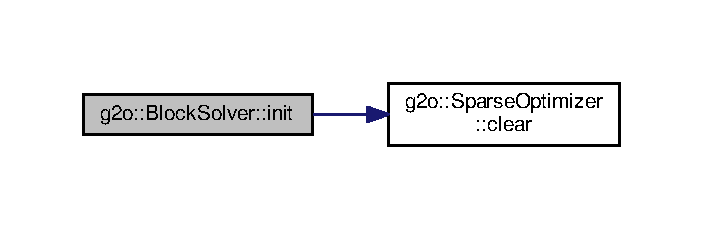
\includegraphics[width=338pt]{classg2o_1_1BlockSolver_a8bf01018abc3bfddfa3b29a380a1d6cb_cgraph}
\end{center}
\end{figure}


\hypertarget{classg2o_1_1BlockSolver_a615892075357273ec8bb06e101d9155b}{\index{g2o\-::\-Block\-Solver@{g2o\-::\-Block\-Solver}!multiply\-Hessian@{multiply\-Hessian}}
\index{multiply\-Hessian@{multiply\-Hessian}!g2o::BlockSolver@{g2o\-::\-Block\-Solver}}
\subsubsection[{multiply\-Hessian}]{\setlength{\rightskip}{0pt plus 5cm}template$<$typename Traits $>$ virtual void {\bf g2o\-::\-Block\-Solver}$<$ Traits $>$\-::multiply\-Hessian (
\begin{DoxyParamCaption}
\item[{double $\ast$}]{dest, }
\item[{const double $\ast$}]{src}
\end{DoxyParamCaption}
) const\hspace{0.3cm}{\ttfamily [inline]}, {\ttfamily [virtual]}}}\label{classg2o_1_1BlockSolver_a615892075357273ec8bb06e101d9155b}
compute dest = H $\ast$ src 

实现了 \hyperlink{classg2o_1_1BlockSolverBase_a4ff7072751bfa1b7fcf91f8219e18e13}{g2o\-::\-Block\-Solver\-Base}.



在文件 block\-\_\-solver.\-h 第 142 行定义.

\hypertarget{classg2o_1_1BlockSolver_a2136931d7aa2f54df5207556c4685809}{\index{g2o\-::\-Block\-Solver@{g2o\-::\-Block\-Solver}!restore\-Diagonal@{restore\-Diagonal}}
\index{restore\-Diagonal@{restore\-Diagonal}!g2o::BlockSolver@{g2o\-::\-Block\-Solver}}
\subsubsection[{restore\-Diagonal}]{\setlength{\rightskip}{0pt plus 5cm}template$<$typename Traits $>$ void {\bf g2o\-::\-Block\-Solver}$<$ Traits $>$\-::restore\-Diagonal (
\begin{DoxyParamCaption}
{}
\end{DoxyParamCaption}
)\hspace{0.3cm}{\ttfamily [virtual]}}}\label{classg2o_1_1BlockSolver_a2136931d7aa2f54df5207556c4685809}
restore a previosly made backup of the diagonal 

实现了 \hyperlink{classg2o_1_1Solver_a3c40dae9b999c4d18e57b02fd0e0ade2}{g2o\-::\-Solver}.



在文件 block\-\_\-solver.\-hpp 第 593 行定义.

\hypertarget{classg2o_1_1BlockSolver_acc63a23e5b35e4f72d46dc22719aa56f}{\index{g2o\-::\-Block\-Solver@{g2o\-::\-Block\-Solver}!set\-Lambda@{set\-Lambda}}
\index{set\-Lambda@{set\-Lambda}!g2o::BlockSolver@{g2o\-::\-Block\-Solver}}
\subsubsection[{set\-Lambda}]{\setlength{\rightskip}{0pt plus 5cm}template$<$typename Traits $>$ bool {\bf g2o\-::\-Block\-Solver}$<$ Traits $>$\-::set\-Lambda (
\begin{DoxyParamCaption}
\item[{double}]{lambda, }
\item[{bool}]{backup = {\ttfamily false}}
\end{DoxyParamCaption}
)\hspace{0.3cm}{\ttfamily [virtual]}}}\label{classg2o_1_1BlockSolver_acc63a23e5b35e4f72d46dc22719aa56f}
update the system while performing Levenberg, i.\-e., modifying the diagonal components of A by doing += lambda along the main diagonal of the Matrix. Note that this function may be called with a positive and a negative lambda. The latter is used to undo a former modification. If backup is true, then the solver should store a backup of the diagonal, which can be restored by \hyperlink{classg2o_1_1BlockSolver_a2136931d7aa2f54df5207556c4685809}{restore\-Diagonal()} 

实现了 \hyperlink{classg2o_1_1Solver_a94a0d5196c7859c6c37fc2368ac56be3}{g2o\-::\-Solver}.



在文件 block\-\_\-solver.\-hpp 第 565 行定义.

\hypertarget{classg2o_1_1BlockSolver_a1bff5dc13e3408fa76c019347104acd0}{\index{g2o\-::\-Block\-Solver@{g2o\-::\-Block\-Solver}!set\-Write\-Debug@{set\-Write\-Debug}}
\index{set\-Write\-Debug@{set\-Write\-Debug}!g2o::BlockSolver@{g2o\-::\-Block\-Solver}}
\subsubsection[{set\-Write\-Debug}]{\setlength{\rightskip}{0pt plus 5cm}template$<$typename Traits $>$ void {\bf g2o\-::\-Block\-Solver}$<$ Traits $>$\-::set\-Write\-Debug (
\begin{DoxyParamCaption}
\item[{bool}]{}
\end{DoxyParamCaption}
)\hspace{0.3cm}{\ttfamily [virtual]}}}\label{classg2o_1_1BlockSolver_a1bff5dc13e3408fa76c019347104acd0}
write debug output of the Hessian if system is not positive definite 

实现了 \hyperlink{classg2o_1_1Solver_ad3ef2a487d991363ba86af2840b0d7cd}{g2o\-::\-Solver}.



在文件 block\-\_\-solver.\-hpp 第 624 行定义.

\hypertarget{classg2o_1_1BlockSolver_a589a75a131cce100c1945ad2786214d7}{\index{g2o\-::\-Block\-Solver@{g2o\-::\-Block\-Solver}!solve@{solve}}
\index{solve@{solve}!g2o::BlockSolver@{g2o\-::\-Block\-Solver}}
\subsubsection[{solve}]{\setlength{\rightskip}{0pt plus 5cm}template$<$typename Traits $>$ bool {\bf g2o\-::\-Block\-Solver}$<$ Traits $>$\-::solve (
\begin{DoxyParamCaption}
{}
\end{DoxyParamCaption}
)\hspace{0.3cm}{\ttfamily [virtual]}}}\label{classg2o_1_1BlockSolver_a589a75a131cce100c1945ad2786214d7}
solve Ax = b 

实现了 \hyperlink{classg2o_1_1Solver_a9c359a886db57f2f81e54a2113f3bd38}{g2o\-::\-Solver}.



在文件 block\-\_\-solver.\-hpp 第 355 行定义.



参考 g2o\-::\-Sparse\-Block\-Matrix\-C\-C\-S$<$ Matrix\-Type $>$\-::block\-Cols(), g2o\-::\-Sparse\-Block\-Matrix$<$ Matrix\-Type $>$\-::block\-Cols(), g2o\-::\-G2\-O\-Batch\-Statistics\-::hessian\-Dimension, g2o\-::\-G2\-O\-Batch\-Statistics\-::hessian\-Landmark\-Dimension, g2o\-::\-G2\-O\-Batch\-Statistics\-::hessian\-Pose\-Dimension, g2o\-::\-G2\-O\-Batch\-Statistics\-::time\-Linear\-Solver , 以及 g2o\-::\-G2\-O\-Batch\-Statistics\-::time\-Schur\-Complement.



函数调用图\-:
\nopagebreak
\begin{figure}[H]
\begin{center}
\leavevmode
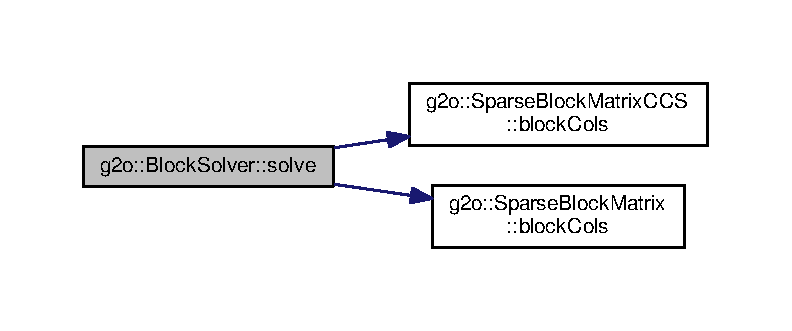
\includegraphics[width=350pt]{classg2o_1_1BlockSolver_a589a75a131cce100c1945ad2786214d7_cgraph}
\end{center}
\end{figure}


\hypertarget{classg2o_1_1BlockSolver_a68dc822ce48e80ceacce69c7bd029674}{\index{g2o\-::\-Block\-Solver@{g2o\-::\-Block\-Solver}!supports\-Schur@{supports\-Schur}}
\index{supports\-Schur@{supports\-Schur}!g2o::BlockSolver@{g2o\-::\-Block\-Solver}}
\subsubsection[{supports\-Schur}]{\setlength{\rightskip}{0pt plus 5cm}template$<$typename Traits $>$ virtual bool {\bf g2o\-::\-Block\-Solver}$<$ Traits $>$\-::supports\-Schur (
\begin{DoxyParamCaption}
{}
\end{DoxyParamCaption}
)\hspace{0.3cm}{\ttfamily [inline]}, {\ttfamily [virtual]}}}\label{classg2o_1_1BlockSolver_a68dc822ce48e80ceacce69c7bd029674}
does this solver support the Schur complement for solving a system consisting of poses and landmarks. Re-\/implemement in a derived solver, if your solver supports it. 

重载 \hyperlink{classg2o_1_1Solver_a36c68f7bc0b8864ee7722bc3c06de554}{g2o\-::\-Solver} .



在文件 block\-\_\-solver.\-h 第 131 行定义.

\hypertarget{classg2o_1_1BlockSolver_acc497239c5e681ddec2140e34dfc5938}{\index{g2o\-::\-Block\-Solver@{g2o\-::\-Block\-Solver}!update\-Structure@{update\-Structure}}
\index{update\-Structure@{update\-Structure}!g2o::BlockSolver@{g2o\-::\-Block\-Solver}}
\subsubsection[{update\-Structure}]{\setlength{\rightskip}{0pt plus 5cm}template$<$typename Traits $>$ bool {\bf g2o\-::\-Block\-Solver}$<$ Traits $>$\-::update\-Structure (
\begin{DoxyParamCaption}
\item[{const std\-::vector$<$ {\bf Hyper\-Graph\-::\-Vertex} $\ast$ $>$ \&}]{vset, }
\item[{const Hyper\-Graph\-::\-Edge\-Set \&}]{edges}
\end{DoxyParamCaption}
)\hspace{0.3cm}{\ttfamily [virtual]}}}\label{classg2o_1_1BlockSolver_acc497239c5e681ddec2140e34dfc5938}
update the structures for online processing 

实现了 \hyperlink{classg2o_1_1Solver_a035b8effea7178eabfb35e1c78b25987}{g2o\-::\-Solver}.



在文件 block\-\_\-solver.\-hpp 第 299 行定义.



参考 g2o\-::\-Optimizable\-Graph\-::\-Vertex\-::dimension(), g2o\-::\-Optimizable\-Graph\-::\-Vertex\-::hessian\-Index(), g2o\-::\-Optimizable\-Graph\-::\-Vertex\-::map\-Hessian\-Memory(), g2o\-::\-Optimizable\-Graph\-::\-Edge\-::map\-Hessian\-Memory(), g2o\-::\-Optimizable\-Graph\-::\-Vertex\-::marginalized(), g2o\-::\-Optimizable\-Graph\-::\-Vertex\-::set\-Col\-In\-Hessian(), g2o\-::\-Hyper\-Graph\-::\-Edge\-::vertex() , 以及 g2o\-::\-Hyper\-Graph\-::\-Edge\-::vertices().



函数调用图\-:
\nopagebreak
\begin{figure}[H]
\begin{center}
\leavevmode
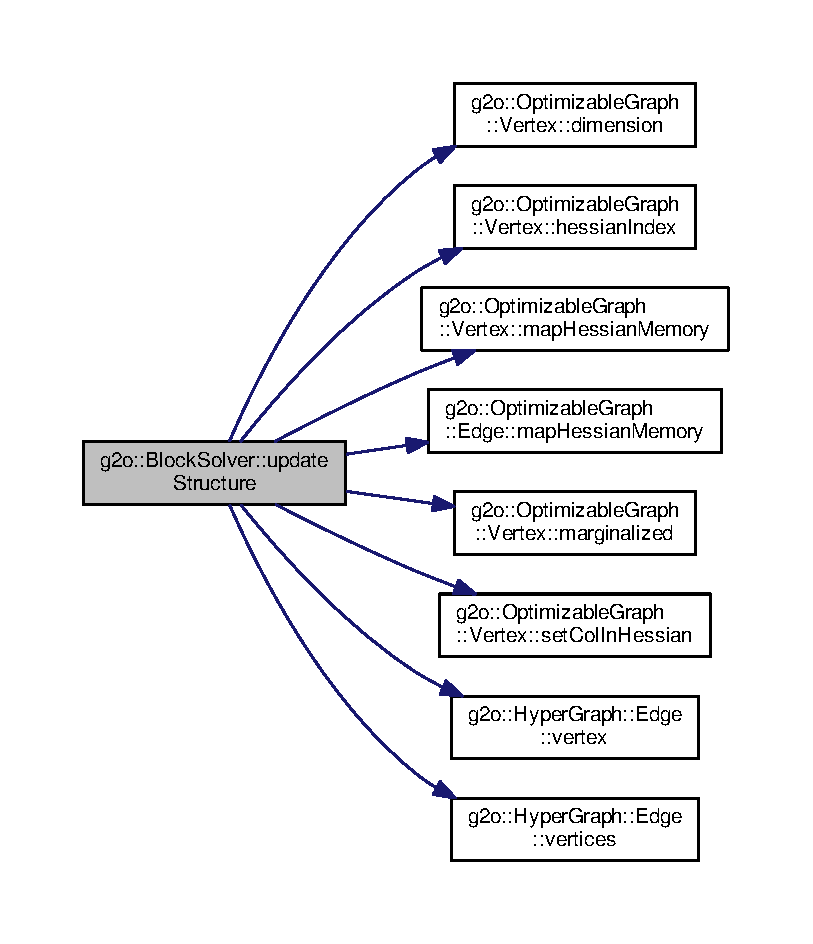
\includegraphics[width=350pt]{classg2o_1_1BlockSolver_acc497239c5e681ddec2140e34dfc5938_cgraph}
\end{center}
\end{figure}




该类的文档由以下文件生成\-:\begin{DoxyCompactItemize}
\item 
Thirdparty/g2o/g2o/core/block\-\_\-solver.\-h\item 
Thirdparty/g2o/g2o/core/block\-\_\-solver.\-hpp\end{DoxyCompactItemize}

\hypertarget{classg2o_1_1BlockSolverBase}{\section{g2o\-:\-:Block\-Solver\-Base类 参考}
\label{classg2o_1_1BlockSolverBase}\index{g2o\-::\-Block\-Solver\-Base@{g2o\-::\-Block\-Solver\-Base}}
}


base for the block solvers with some basic function interfaces  




{\ttfamily \#include $<$block\-\_\-solver.\-h$>$}



类 g2o\-:\-:Block\-Solver\-Base 继承关系图\-:
\nopagebreak
\begin{figure}[H]
\begin{center}
\leavevmode
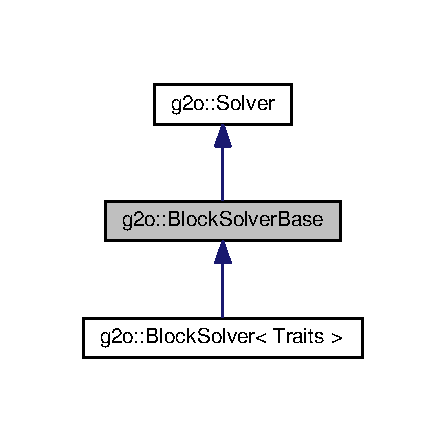
\includegraphics[width=214pt]{classg2o_1_1BlockSolverBase__inherit__graph}
\end{center}
\end{figure}


g2o\-:\-:Block\-Solver\-Base 的协作图\-:
\nopagebreak
\begin{figure}[H]
\begin{center}
\leavevmode
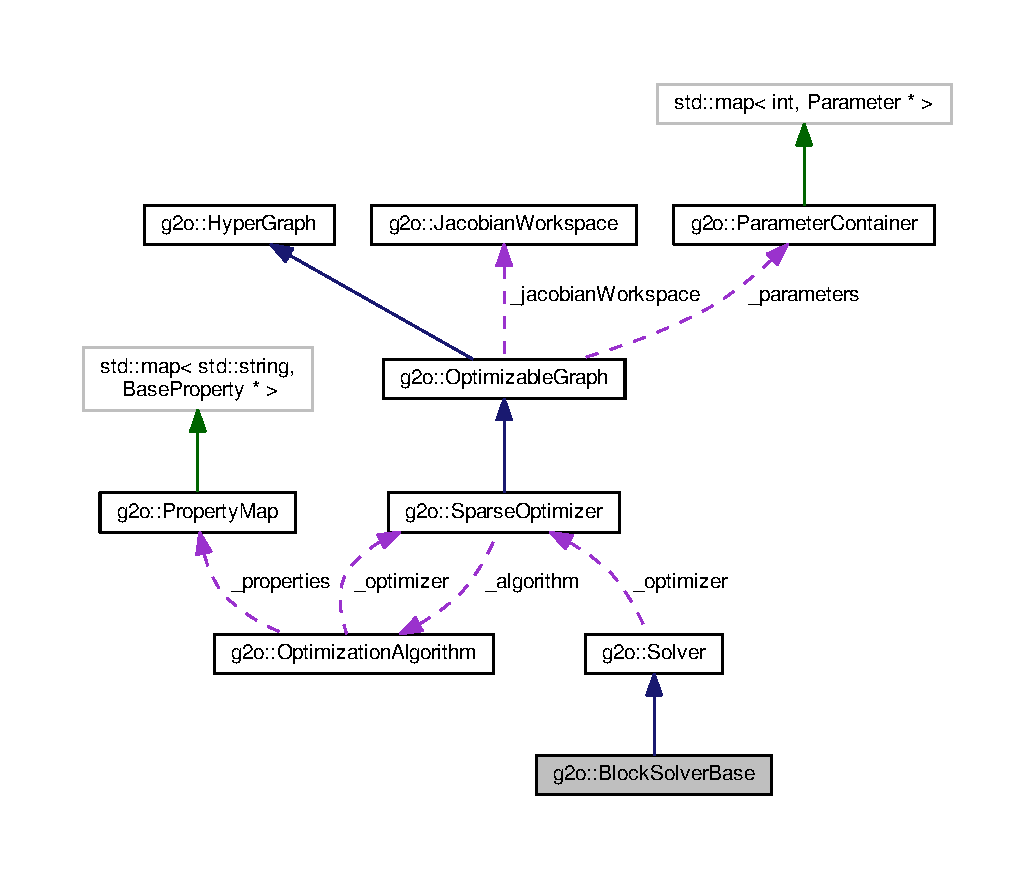
\includegraphics[width=350pt]{classg2o_1_1BlockSolverBase__coll__graph}
\end{center}
\end{figure}
\subsection*{Public 成员函数}
\begin{DoxyCompactItemize}
\item 
virtual void \hyperlink{classg2o_1_1BlockSolverBase_a4ff7072751bfa1b7fcf91f8219e18e13}{multiply\-Hessian} (double $\ast$dest, const double $\ast$src) const =0
\end{DoxyCompactItemize}
\subsection*{额外继承的成员函数}


\subsection{详细描述}
base for the block solvers with some basic function interfaces 

在文件 block\-\_\-solver.\-h 第 83 行定义.



\subsection{成员函数说明}
\hypertarget{classg2o_1_1BlockSolverBase_a4ff7072751bfa1b7fcf91f8219e18e13}{\index{g2o\-::\-Block\-Solver\-Base@{g2o\-::\-Block\-Solver\-Base}!multiply\-Hessian@{multiply\-Hessian}}
\index{multiply\-Hessian@{multiply\-Hessian}!g2o::BlockSolverBase@{g2o\-::\-Block\-Solver\-Base}}
\subsubsection[{multiply\-Hessian}]{\setlength{\rightskip}{0pt plus 5cm}virtual void g2o\-::\-Block\-Solver\-Base\-::multiply\-Hessian (
\begin{DoxyParamCaption}
\item[{double $\ast$}]{dest, }
\item[{const double $\ast$}]{src}
\end{DoxyParamCaption}
) const\hspace{0.3cm}{\ttfamily [pure virtual]}}}\label{classg2o_1_1BlockSolverBase_a4ff7072751bfa1b7fcf91f8219e18e13}
compute dest = H $\ast$ src 

在 \hyperlink{classg2o_1_1BlockSolver_a615892075357273ec8bb06e101d9155b}{g2o\-::\-Block\-Solver$<$ Traits $>$} 内被实现.



参考自 g2o\-::\-Optimization\-Algorithm\-Dogleg\-::solve().



这是这个函数的调用关系图\-:
\nopagebreak
\begin{figure}[H]
\begin{center}
\leavevmode
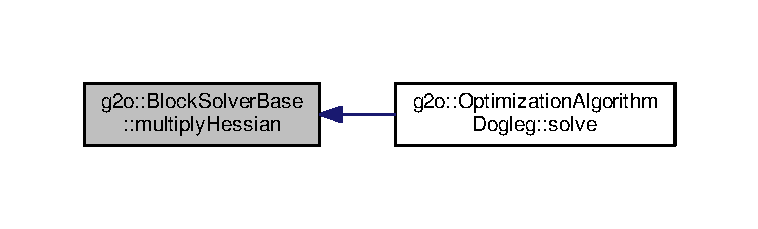
\includegraphics[width=350pt]{classg2o_1_1BlockSolverBase_a4ff7072751bfa1b7fcf91f8219e18e13_icgraph}
\end{center}
\end{figure}




该类的文档由以下文件生成\-:\begin{DoxyCompactItemize}
\item 
Thirdparty/g2o/g2o/core/block\-\_\-solver.\-h\end{DoxyCompactItemize}

\hypertarget{structg2o_1_1BlockSolverTraits}{\section{g2o\-:\-:Block\-Solver\-Traits$<$ \-\_\-\-Pose\-Dim, \-\_\-\-Landmark\-Dim $>$ 模板结构体 参考}
\label{structg2o_1_1BlockSolverTraits}\index{g2o\-::\-Block\-Solver\-Traits$<$ \-\_\-\-Pose\-Dim, \-\_\-\-Landmark\-Dim $>$@{g2o\-::\-Block\-Solver\-Traits$<$ \-\_\-\-Pose\-Dim, \-\_\-\-Landmark\-Dim $>$}}
}


traits to summarize the properties of the fixed size optimization problem  




{\ttfamily \#include $<$block\-\_\-solver.\-h$>$}

\subsection*{Public 类型}
\begin{DoxyCompactItemize}
\item 
\hypertarget{structg2o_1_1BlockSolverTraits_a35e6e4bad138dcfcaa3b1339e168bf30}{typedef Matrix$<$ double, \\*
Pose\-Dim, Pose\-Dim $>$ {\bfseries Pose\-Matrix\-Type}}\label{structg2o_1_1BlockSolverTraits_a35e6e4bad138dcfcaa3b1339e168bf30}

\item 
\hypertarget{structg2o_1_1BlockSolverTraits_add9b9fbfef352b7654d41914d5eaa58c}{typedef Matrix$<$ double, \\*
Landmark\-Dim, Landmark\-Dim $>$ {\bfseries Landmark\-Matrix\-Type}}\label{structg2o_1_1BlockSolverTraits_add9b9fbfef352b7654d41914d5eaa58c}

\item 
\hypertarget{structg2o_1_1BlockSolverTraits_a91e6510ad42179701d22c3ac312237cd}{typedef Matrix$<$ double, \\*
Pose\-Dim, Landmark\-Dim $>$ {\bfseries Pose\-Landmark\-Matrix\-Type}}\label{structg2o_1_1BlockSolverTraits_a91e6510ad42179701d22c3ac312237cd}

\item 
\hypertarget{structg2o_1_1BlockSolverTraits_a032ed57e9bc44c36093f97b32e1506f6}{typedef Matrix$<$ double, \\*
Pose\-Dim, 1 $>$ {\bfseries Pose\-Vector\-Type}}\label{structg2o_1_1BlockSolverTraits_a032ed57e9bc44c36093f97b32e1506f6}

\item 
\hypertarget{structg2o_1_1BlockSolverTraits_af5154a15abb566ff5bffc0adb9f0458d}{typedef Matrix$<$ double, \\*
Landmark\-Dim, 1 $>$ {\bfseries Landmark\-Vector\-Type}}\label{structg2o_1_1BlockSolverTraits_af5154a15abb566ff5bffc0adb9f0458d}

\item 
\hypertarget{structg2o_1_1BlockSolverTraits_a03351362339d8e6609c577123350bb2a}{typedef \hyperlink{classg2o_1_1SparseBlockMatrix}{Sparse\-Block\-Matrix}\\*
$<$ Pose\-Matrix\-Type $>$ {\bfseries Pose\-Hessian\-Type}}\label{structg2o_1_1BlockSolverTraits_a03351362339d8e6609c577123350bb2a}

\item 
\hypertarget{structg2o_1_1BlockSolverTraits_ae761bb32d5267e4d74e5d9c2c7e7ad2f}{typedef \hyperlink{classg2o_1_1SparseBlockMatrix}{Sparse\-Block\-Matrix}\\*
$<$ Landmark\-Matrix\-Type $>$ {\bfseries Landmark\-Hessian\-Type}}\label{structg2o_1_1BlockSolverTraits_ae761bb32d5267e4d74e5d9c2c7e7ad2f}

\item 
\hypertarget{structg2o_1_1BlockSolverTraits_af8ef27915a056caae3b12a9ca609eba6}{typedef \hyperlink{classg2o_1_1SparseBlockMatrix}{Sparse\-Block\-Matrix}\\*
$<$ Pose\-Landmark\-Matrix\-Type $>$ {\bfseries Pose\-Landmark\-Hessian\-Type}}\label{structg2o_1_1BlockSolverTraits_af8ef27915a056caae3b12a9ca609eba6}

\item 
\hypertarget{structg2o_1_1BlockSolverTraits_add6edae08cb0665c2b1e7c641cdb4dc4}{typedef \hyperlink{classg2o_1_1LinearSolver}{Linear\-Solver}\\*
$<$ Pose\-Matrix\-Type $>$ {\bfseries Linear\-Solver\-Type}}\label{structg2o_1_1BlockSolverTraits_add6edae08cb0665c2b1e7c641cdb4dc4}

\end{DoxyCompactItemize}
\subsection*{静态 Public 属性}
\begin{DoxyCompactItemize}
\item 
\hypertarget{structg2o_1_1BlockSolverTraits_a90a03bcfc60b629da5601f6df9514297}{static const int {\bfseries Pose\-Dim} = \-\_\-\-Pose\-Dim}\label{structg2o_1_1BlockSolverTraits_a90a03bcfc60b629da5601f6df9514297}

\item 
\hypertarget{structg2o_1_1BlockSolverTraits_a7e6e33971e5243e020a9f41cd3182218}{static const int {\bfseries Landmark\-Dim} = \-\_\-\-Landmark\-Dim}\label{structg2o_1_1BlockSolverTraits_a7e6e33971e5243e020a9f41cd3182218}

\end{DoxyCompactItemize}


\subsection{详细描述}
\subsubsection*{template$<$int \-\_\-\-Pose\-Dim, int \-\_\-\-Landmark\-Dim$>$struct g2o\-::\-Block\-Solver\-Traits$<$ \-\_\-\-Pose\-Dim, \-\_\-\-Landmark\-Dim $>$}

traits to summarize the properties of the fixed size optimization problem 

在文件 block\-\_\-solver.\-h 第 44 行定义.



该结构体的文档由以下文件生成\-:\begin{DoxyCompactItemize}
\item 
Thirdparty/g2o/g2o/core/block\-\_\-solver.\-h\end{DoxyCompactItemize}

\hypertarget{structg2o_1_1BlockSolverTraits_3_01Eigen_1_1Dynamic_00_01Eigen_1_1Dynamic_01_4}{\section{g2o\-:\-:Block\-Solver\-Traits$<$ Eigen\-:\-:Dynamic, Eigen\-:\-:Dynamic $>$ 模板结构体 参考}
\label{structg2o_1_1BlockSolverTraits_3_01Eigen_1_1Dynamic_00_01Eigen_1_1Dynamic_01_4}\index{g2o\-::\-Block\-Solver\-Traits$<$ Eigen\-::\-Dynamic, Eigen\-::\-Dynamic $>$@{g2o\-::\-Block\-Solver\-Traits$<$ Eigen\-::\-Dynamic, Eigen\-::\-Dynamic $>$}}
}


traits to summarize the properties of the dynamic size optimization problem  




{\ttfamily \#include $<$block\-\_\-solver.\-h$>$}

\subsection*{Public 类型}
\begin{DoxyCompactItemize}
\item 
\hypertarget{structg2o_1_1BlockSolverTraits_3_01Eigen_1_1Dynamic_00_01Eigen_1_1Dynamic_01_4_a11131d4b2d25cea90eef0d3687eb6dc1}{typedef Matrix\-Xd {\bfseries Pose\-Matrix\-Type}}\label{structg2o_1_1BlockSolverTraits_3_01Eigen_1_1Dynamic_00_01Eigen_1_1Dynamic_01_4_a11131d4b2d25cea90eef0d3687eb6dc1}

\item 
\hypertarget{structg2o_1_1BlockSolverTraits_3_01Eigen_1_1Dynamic_00_01Eigen_1_1Dynamic_01_4_a4409de5074b3458f33ba2015e2fa6891}{typedef Matrix\-Xd {\bfseries Landmark\-Matrix\-Type}}\label{structg2o_1_1BlockSolverTraits_3_01Eigen_1_1Dynamic_00_01Eigen_1_1Dynamic_01_4_a4409de5074b3458f33ba2015e2fa6891}

\item 
\hypertarget{structg2o_1_1BlockSolverTraits_3_01Eigen_1_1Dynamic_00_01Eigen_1_1Dynamic_01_4_ab81ac9673971ec5c896f4b431ae30f0b}{typedef Matrix\-Xd {\bfseries Pose\-Landmark\-Matrix\-Type}}\label{structg2o_1_1BlockSolverTraits_3_01Eigen_1_1Dynamic_00_01Eigen_1_1Dynamic_01_4_ab81ac9673971ec5c896f4b431ae30f0b}

\item 
\hypertarget{structg2o_1_1BlockSolverTraits_3_01Eigen_1_1Dynamic_00_01Eigen_1_1Dynamic_01_4_ae8ae50131f5aeaf97c844e20960ebaf3}{typedef Vector\-Xd {\bfseries Pose\-Vector\-Type}}\label{structg2o_1_1BlockSolverTraits_3_01Eigen_1_1Dynamic_00_01Eigen_1_1Dynamic_01_4_ae8ae50131f5aeaf97c844e20960ebaf3}

\item 
\hypertarget{structg2o_1_1BlockSolverTraits_3_01Eigen_1_1Dynamic_00_01Eigen_1_1Dynamic_01_4_aaff14917064b8670c918e571fcdc4666}{typedef Vector\-Xd {\bfseries Landmark\-Vector\-Type}}\label{structg2o_1_1BlockSolverTraits_3_01Eigen_1_1Dynamic_00_01Eigen_1_1Dynamic_01_4_aaff14917064b8670c918e571fcdc4666}

\item 
\hypertarget{structg2o_1_1BlockSolverTraits_3_01Eigen_1_1Dynamic_00_01Eigen_1_1Dynamic_01_4_a380bde2a88f9b257142dd3419422e5a3}{typedef \hyperlink{classg2o_1_1SparseBlockMatrix}{Sparse\-Block\-Matrix}\\*
$<$ Pose\-Matrix\-Type $>$ {\bfseries Pose\-Hessian\-Type}}\label{structg2o_1_1BlockSolverTraits_3_01Eigen_1_1Dynamic_00_01Eigen_1_1Dynamic_01_4_a380bde2a88f9b257142dd3419422e5a3}

\item 
\hypertarget{structg2o_1_1BlockSolverTraits_3_01Eigen_1_1Dynamic_00_01Eigen_1_1Dynamic_01_4_a73a81a0aeabd1216ae3a8f5700666ac4}{typedef \hyperlink{classg2o_1_1SparseBlockMatrix}{Sparse\-Block\-Matrix}\\*
$<$ Landmark\-Matrix\-Type $>$ {\bfseries Landmark\-Hessian\-Type}}\label{structg2o_1_1BlockSolverTraits_3_01Eigen_1_1Dynamic_00_01Eigen_1_1Dynamic_01_4_a73a81a0aeabd1216ae3a8f5700666ac4}

\item 
\hypertarget{structg2o_1_1BlockSolverTraits_3_01Eigen_1_1Dynamic_00_01Eigen_1_1Dynamic_01_4_aa6f67fd6ba29156f6d1069db0c3b5d11}{typedef \hyperlink{classg2o_1_1SparseBlockMatrix}{Sparse\-Block\-Matrix}\\*
$<$ Pose\-Landmark\-Matrix\-Type $>$ {\bfseries Pose\-Landmark\-Hessian\-Type}}\label{structg2o_1_1BlockSolverTraits_3_01Eigen_1_1Dynamic_00_01Eigen_1_1Dynamic_01_4_aa6f67fd6ba29156f6d1069db0c3b5d11}

\item 
\hypertarget{structg2o_1_1BlockSolverTraits_3_01Eigen_1_1Dynamic_00_01Eigen_1_1Dynamic_01_4_ad062ca3c21bf3a3e08d5350174d93d6d}{typedef \hyperlink{classg2o_1_1LinearSolver}{Linear\-Solver}\\*
$<$ Pose\-Matrix\-Type $>$ {\bfseries Linear\-Solver\-Type}}\label{structg2o_1_1BlockSolverTraits_3_01Eigen_1_1Dynamic_00_01Eigen_1_1Dynamic_01_4_ad062ca3c21bf3a3e08d5350174d93d6d}

\end{DoxyCompactItemize}
\subsection*{静态 Public 属性}
\begin{DoxyCompactItemize}
\item 
\hypertarget{structg2o_1_1BlockSolverTraits_3_01Eigen_1_1Dynamic_00_01Eigen_1_1Dynamic_01_4_a04a2cc2de80563b4b21f815150c3b0ec}{static const int {\bfseries Pose\-Dim} = Eigen\-::\-Dynamic}\label{structg2o_1_1BlockSolverTraits_3_01Eigen_1_1Dynamic_00_01Eigen_1_1Dynamic_01_4_a04a2cc2de80563b4b21f815150c3b0ec}

\item 
\hypertarget{structg2o_1_1BlockSolverTraits_3_01Eigen_1_1Dynamic_00_01Eigen_1_1Dynamic_01_4_aa8f7b7c3fc1ce4a7d61e925e3067e196}{static const int {\bfseries Landmark\-Dim} = Eigen\-::\-Dynamic}\label{structg2o_1_1BlockSolverTraits_3_01Eigen_1_1Dynamic_00_01Eigen_1_1Dynamic_01_4_aa8f7b7c3fc1ce4a7d61e925e3067e196}

\end{DoxyCompactItemize}


\subsection{详细描述}
\subsubsection*{template$<$$>$struct g2o\-::\-Block\-Solver\-Traits$<$ Eigen\-::\-Dynamic, Eigen\-::\-Dynamic $>$}

traits to summarize the properties of the dynamic size optimization problem 

在文件 block\-\_\-solver.\-h 第 64 行定义.



该结构体的文档由以下文件生成\-:\begin{DoxyCompactItemize}
\item 
Thirdparty/g2o/g2o/core/block\-\_\-solver.\-h\end{DoxyCompactItemize}

\hypertarget{classDBoW2_1_1BowVector}{\section{D\-Bo\-W2\-:\-:Bow\-Vector类 参考}
\label{classDBoW2_1_1BowVector}\index{D\-Bo\-W2\-::\-Bow\-Vector@{D\-Bo\-W2\-::\-Bow\-Vector}}
}


{\ttfamily \#include $<$Bow\-Vector.\-h$>$}



类 D\-Bo\-W2\-:\-:Bow\-Vector 继承关系图\-:
\nopagebreak
\begin{figure}[H]
\begin{center}
\leavevmode
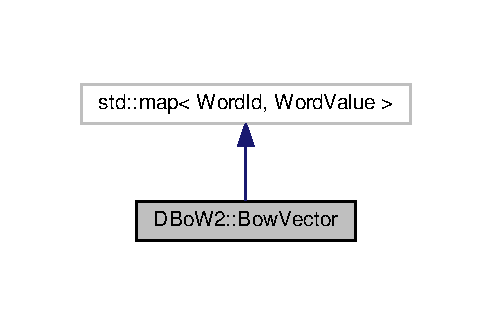
\includegraphics[width=236pt]{classDBoW2_1_1BowVector__inherit__graph}
\end{center}
\end{figure}


D\-Bo\-W2\-:\-:Bow\-Vector 的协作图\-:
\nopagebreak
\begin{figure}[H]
\begin{center}
\leavevmode
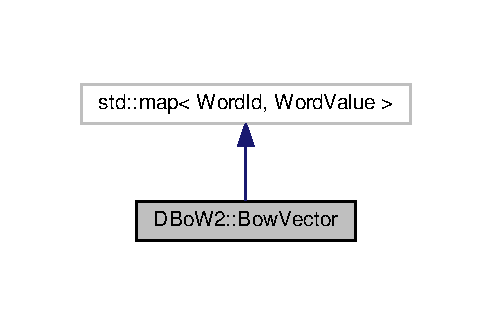
\includegraphics[width=236pt]{classDBoW2_1_1BowVector__coll__graph}
\end{center}
\end{figure}
\subsection*{Public 成员函数}
\begin{DoxyCompactItemize}
\item 
\hyperlink{classDBoW2_1_1BowVector_ac4da23e700adc4ee083d66b23ce86e90}{Bow\-Vector} (void)
\item 
\hyperlink{classDBoW2_1_1BowVector_a7210cac6ce006c7232f4d097faa338d0}{$\sim$\-Bow\-Vector} (void)
\item 
void \hyperlink{classDBoW2_1_1BowVector_a3ac92a805b252c93dc6535240d02df47}{add\-Weight} (\hyperlink{namespaceDBoW2_ab1a0d3283b2d4690a383372ed20bfeb5}{Word\-Id} id, \hyperlink{namespaceDBoW2_a55fcd7333e591a38e96b91f41bc182f6}{Word\-Value} v)
\item 
void \hyperlink{classDBoW2_1_1BowVector_a5ddf10e444d10425e5bd3568dc7ffe5e}{add\-If\-Not\-Exist} (\hyperlink{namespaceDBoW2_ab1a0d3283b2d4690a383372ed20bfeb5}{Word\-Id} id, \hyperlink{namespaceDBoW2_a55fcd7333e591a38e96b91f41bc182f6}{Word\-Value} v)
\item 
void \hyperlink{classDBoW2_1_1BowVector_acd2dd34023e3053a4cc75d70c8b6ac13}{normalize} (\hyperlink{namespaceDBoW2_a53e9e0bcfc25c861815e413a7cf3fa51}{L\-Norm} norm\-\_\-type)
\item 
void \hyperlink{classDBoW2_1_1BowVector_af15c4fde81b89e0f76a00337883b6b4a}{save\-M} (const std\-::string \&filename, size\-\_\-t W) const 
\end{DoxyCompactItemize}
\subsection*{友元}
\begin{DoxyCompactItemize}
\item 
std\-::ostream \& \hyperlink{classDBoW2_1_1BowVector_a1a7d9ac0f9128538859adfea38453ae1}{operator$<$$<$} (std\-::ostream \&out, const \hyperlink{classDBoW2_1_1BowVector}{Bow\-Vector} \&v)
\end{DoxyCompactItemize}


\subsection{详细描述}
Vector of words to represent images stl的map结构,key为word\-Id,value为tfidf中的tf 

在文件 Bow\-Vector.\-h 第 59 行定义.



\subsection{构造及析构函数说明}
\hypertarget{classDBoW2_1_1BowVector_ac4da23e700adc4ee083d66b23ce86e90}{\index{D\-Bo\-W2\-::\-Bow\-Vector@{D\-Bo\-W2\-::\-Bow\-Vector}!Bow\-Vector@{Bow\-Vector}}
\index{Bow\-Vector@{Bow\-Vector}!DBoW2::BowVector@{D\-Bo\-W2\-::\-Bow\-Vector}}
\subsubsection[{Bow\-Vector}]{\setlength{\rightskip}{0pt plus 5cm}D\-Bo\-W2\-::\-Bow\-Vector\-::\-Bow\-Vector (
\begin{DoxyParamCaption}
\item[{void}]{}
\end{DoxyParamCaption}
)}}\label{classDBoW2_1_1BowVector_ac4da23e700adc4ee083d66b23ce86e90}
Constructor 

在文件 Bow\-Vector.\-cpp 第 22 行定义.

\hypertarget{classDBoW2_1_1BowVector_a7210cac6ce006c7232f4d097faa338d0}{\index{D\-Bo\-W2\-::\-Bow\-Vector@{D\-Bo\-W2\-::\-Bow\-Vector}!$\sim$\-Bow\-Vector@{$\sim$\-Bow\-Vector}}
\index{$\sim$\-Bow\-Vector@{$\sim$\-Bow\-Vector}!DBoW2::BowVector@{D\-Bo\-W2\-::\-Bow\-Vector}}
\subsubsection[{$\sim$\-Bow\-Vector}]{\setlength{\rightskip}{0pt plus 5cm}D\-Bo\-W2\-::\-Bow\-Vector\-::$\sim$\-Bow\-Vector (
\begin{DoxyParamCaption}
\item[{void}]{}
\end{DoxyParamCaption}
)}}\label{classDBoW2_1_1BowVector_a7210cac6ce006c7232f4d097faa338d0}
Destructor 

在文件 Bow\-Vector.\-cpp 第 28 行定义.



\subsection{成员函数说明}
\hypertarget{classDBoW2_1_1BowVector_a5ddf10e444d10425e5bd3568dc7ffe5e}{\index{D\-Bo\-W2\-::\-Bow\-Vector@{D\-Bo\-W2\-::\-Bow\-Vector}!add\-If\-Not\-Exist@{add\-If\-Not\-Exist}}
\index{add\-If\-Not\-Exist@{add\-If\-Not\-Exist}!DBoW2::BowVector@{D\-Bo\-W2\-::\-Bow\-Vector}}
\subsubsection[{add\-If\-Not\-Exist}]{\setlength{\rightskip}{0pt plus 5cm}void D\-Bo\-W2\-::\-Bow\-Vector\-::add\-If\-Not\-Exist (
\begin{DoxyParamCaption}
\item[{{\bf Word\-Id}}]{id, }
\item[{{\bf Word\-Value}}]{v}
\end{DoxyParamCaption}
)}}\label{classDBoW2_1_1BowVector_a5ddf10e444d10425e5bd3568dc7ffe5e}
Adds a word with a value to the vector only if this does not exist yet 
\begin{DoxyParams}{参数}
{\em id} & word id to look for \\
\hline
{\em v} & value to give to the word if this does not exist \\
\hline
\end{DoxyParams}


在文件 Bow\-Vector.\-cpp 第 50 行定义.



参考自 D\-Bo\-W2\-::\-Templated\-Vocabulary$<$ T\-Descriptor, F $>$\-::transform().



这是这个函数的调用关系图\-:
\nopagebreak
\begin{figure}[H]
\begin{center}
\leavevmode
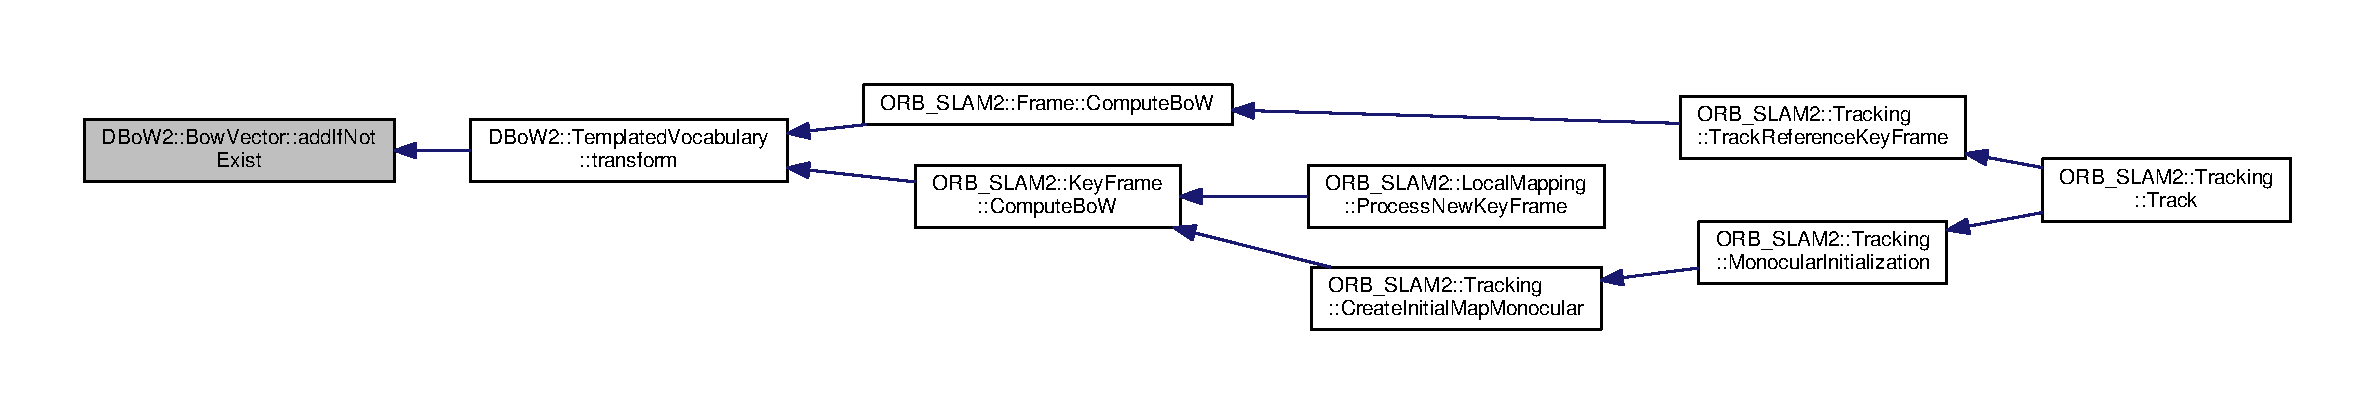
\includegraphics[width=350pt]{classDBoW2_1_1BowVector_a5ddf10e444d10425e5bd3568dc7ffe5e_icgraph}
\end{center}
\end{figure}


\hypertarget{classDBoW2_1_1BowVector_a3ac92a805b252c93dc6535240d02df47}{\index{D\-Bo\-W2\-::\-Bow\-Vector@{D\-Bo\-W2\-::\-Bow\-Vector}!add\-Weight@{add\-Weight}}
\index{add\-Weight@{add\-Weight}!DBoW2::BowVector@{D\-Bo\-W2\-::\-Bow\-Vector}}
\subsubsection[{add\-Weight}]{\setlength{\rightskip}{0pt plus 5cm}void D\-Bo\-W2\-::\-Bow\-Vector\-::add\-Weight (
\begin{DoxyParamCaption}
\item[{{\bf Word\-Id}}]{id, }
\item[{{\bf Word\-Value}}]{v}
\end{DoxyParamCaption}
)}}\label{classDBoW2_1_1BowVector_a3ac92a805b252c93dc6535240d02df47}
Adds a value to a word value existing in the vector, or creates a new word with the given value 
\begin{DoxyParams}{参数}
{\em id} & word id to look for \\
\hline
{\em v} & value to create the word with, or to add to existing word \\
\hline
\end{DoxyParams}


在文件 Bow\-Vector.\-cpp 第 34 行定义.



参考自 D\-Bo\-W2\-::\-Templated\-Vocabulary$<$ T\-Descriptor, F $>$\-::transform().



这是这个函数的调用关系图\-:
\nopagebreak
\begin{figure}[H]
\begin{center}
\leavevmode
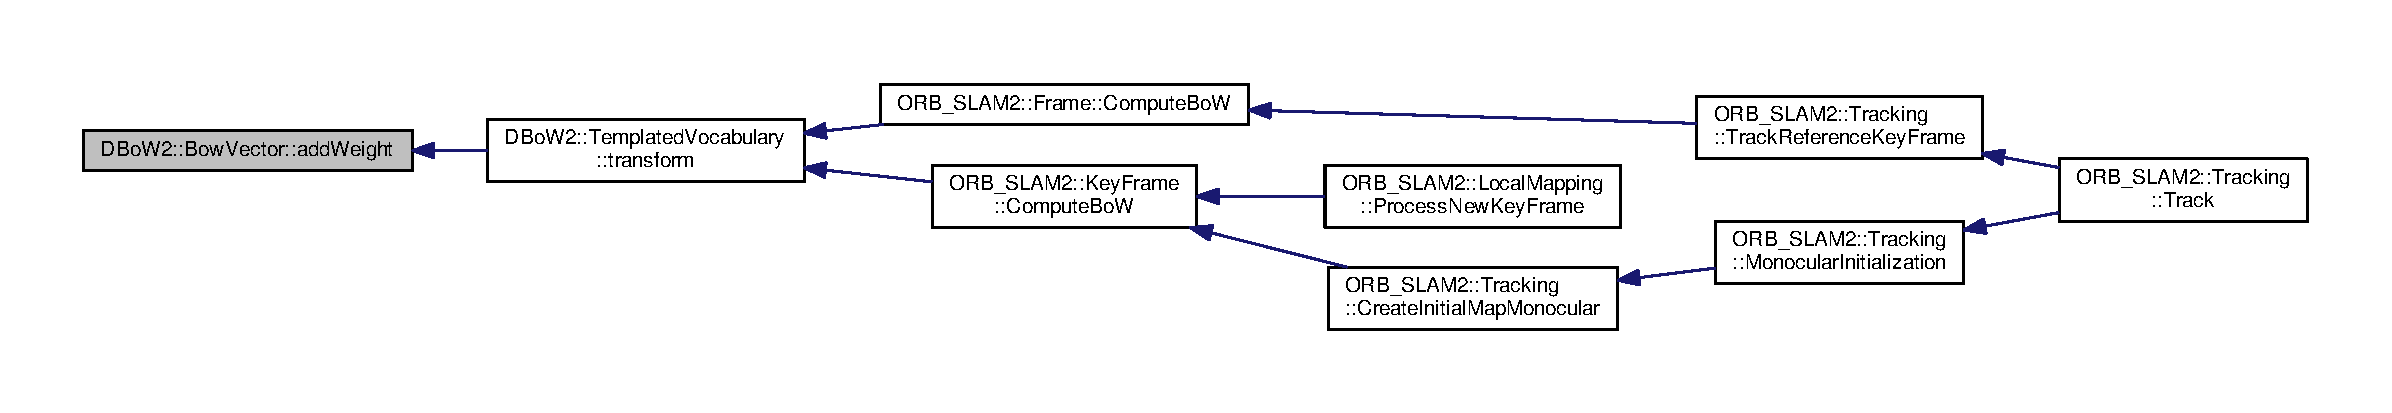
\includegraphics[width=350pt]{classDBoW2_1_1BowVector_a3ac92a805b252c93dc6535240d02df47_icgraph}
\end{center}
\end{figure}


\hypertarget{classDBoW2_1_1BowVector_acd2dd34023e3053a4cc75d70c8b6ac13}{\index{D\-Bo\-W2\-::\-Bow\-Vector@{D\-Bo\-W2\-::\-Bow\-Vector}!normalize@{normalize}}
\index{normalize@{normalize}!DBoW2::BowVector@{D\-Bo\-W2\-::\-Bow\-Vector}}
\subsubsection[{normalize}]{\setlength{\rightskip}{0pt plus 5cm}void D\-Bo\-W2\-::\-Bow\-Vector\-::normalize (
\begin{DoxyParamCaption}
\item[{{\bf L\-Norm}}]{norm\-\_\-type}
\end{DoxyParamCaption}
)}}\label{classDBoW2_1_1BowVector_acd2dd34023e3053a4cc75d70c8b6ac13}
L1-\/\-Normalizes the values in the vector 
\begin{DoxyParams}{参数}
{\em norm\-\_\-type} & norm used \\
\hline
\end{DoxyParams}


在文件 Bow\-Vector.\-cpp 第 62 行定义.



参考自 D\-Bo\-W2\-::\-Templated\-Vocabulary$<$ T\-Descriptor, F $>$\-::transform().



这是这个函数的调用关系图\-:
\nopagebreak
\begin{figure}[H]
\begin{center}
\leavevmode
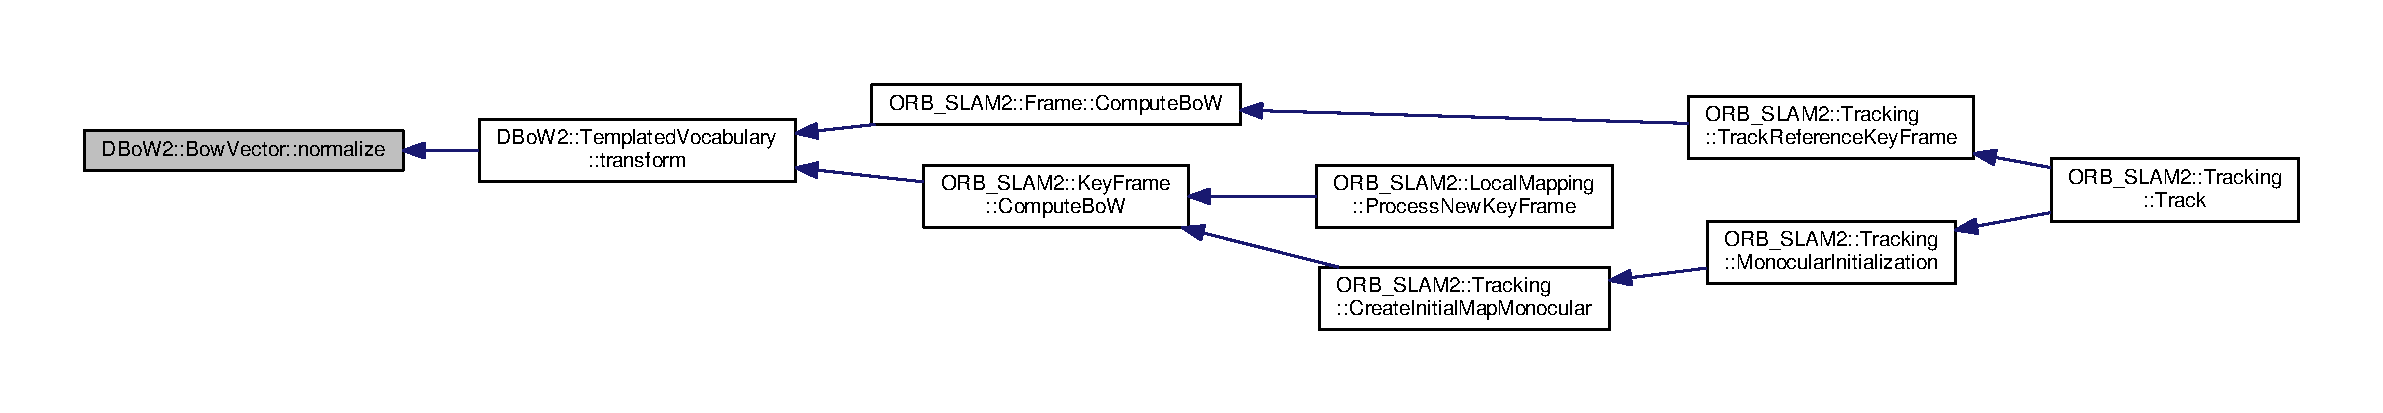
\includegraphics[width=350pt]{classDBoW2_1_1BowVector_acd2dd34023e3053a4cc75d70c8b6ac13_icgraph}
\end{center}
\end{figure}


\hypertarget{classDBoW2_1_1BowVector_af15c4fde81b89e0f76a00337883b6b4a}{\index{D\-Bo\-W2\-::\-Bow\-Vector@{D\-Bo\-W2\-::\-Bow\-Vector}!save\-M@{save\-M}}
\index{save\-M@{save\-M}!DBoW2::BowVector@{D\-Bo\-W2\-::\-Bow\-Vector}}
\subsubsection[{save\-M}]{\setlength{\rightskip}{0pt plus 5cm}void D\-Bo\-W2\-::\-Bow\-Vector\-::save\-M (
\begin{DoxyParamCaption}
\item[{const std\-::string \&}]{filename, }
\item[{size\-\_\-t}]{W}
\end{DoxyParamCaption}
) const}}\label{classDBoW2_1_1BowVector_af15c4fde81b89e0f76a00337883b6b4a}
Saves the bow vector as a vector in a matlab file 
\begin{DoxyParams}{参数}
{\em filename} & \\
\hline
{\em W} & number of words in the vocabulary \\
\hline
\end{DoxyParams}


在文件 Bow\-Vector.\-cpp 第 105 行定义.



\subsection{友元及相关函数文档}
\hypertarget{classDBoW2_1_1BowVector_a1a7d9ac0f9128538859adfea38453ae1}{\index{D\-Bo\-W2\-::\-Bow\-Vector@{D\-Bo\-W2\-::\-Bow\-Vector}!operator$<$$<$@{operator$<$$<$}}
\index{operator$<$$<$@{operator$<$$<$}!DBoW2::BowVector@{D\-Bo\-W2\-::\-Bow\-Vector}}
\subsubsection[{operator$<$$<$}]{\setlength{\rightskip}{0pt plus 5cm}std\-::ostream\& operator$<$$<$ (
\begin{DoxyParamCaption}
\item[{std\-::ostream \&}]{out, }
\item[{const {\bf Bow\-Vector} \&}]{v}
\end{DoxyParamCaption}
)\hspace{0.3cm}{\ttfamily [friend]}}}\label{classDBoW2_1_1BowVector_a1a7d9ac0f9128538859adfea38453ae1}
Prints the content of the bow vector 
\begin{DoxyParams}{参数}
{\em out} & stream \\
\hline
{\em v} & \\
\hline
\end{DoxyParams}


在文件 Bow\-Vector.\-cpp 第 88 行定义.



该类的文档由以下文件生成\-:\begin{DoxyCompactItemize}
\item 
Thirdparty/\-D\-Bo\-W2/\-D\-Bo\-W2/Bow\-Vector.\-h\item 
Thirdparty/\-D\-Bo\-W2/\-D\-Bo\-W2/Bow\-Vector.\-cpp\end{DoxyCompactItemize}

\hypertarget{classg2o_1_1Cache}{\section{g2o\-:\-:Cache类 参考}
\label{classg2o_1_1Cache}\index{g2o\-::\-Cache@{g2o\-::\-Cache}}
}


类 g2o\-:\-:Cache 继承关系图\-:
\nopagebreak
\begin{figure}[H]
\begin{center}
\leavevmode
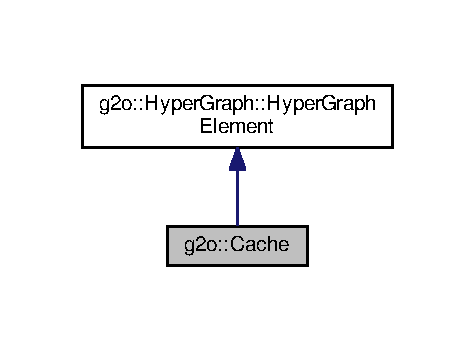
\includegraphics[width=228pt]{classg2o_1_1Cache__inherit__graph}
\end{center}
\end{figure}


g2o\-:\-:Cache 的协作图\-:
\nopagebreak
\begin{figure}[H]
\begin{center}
\leavevmode
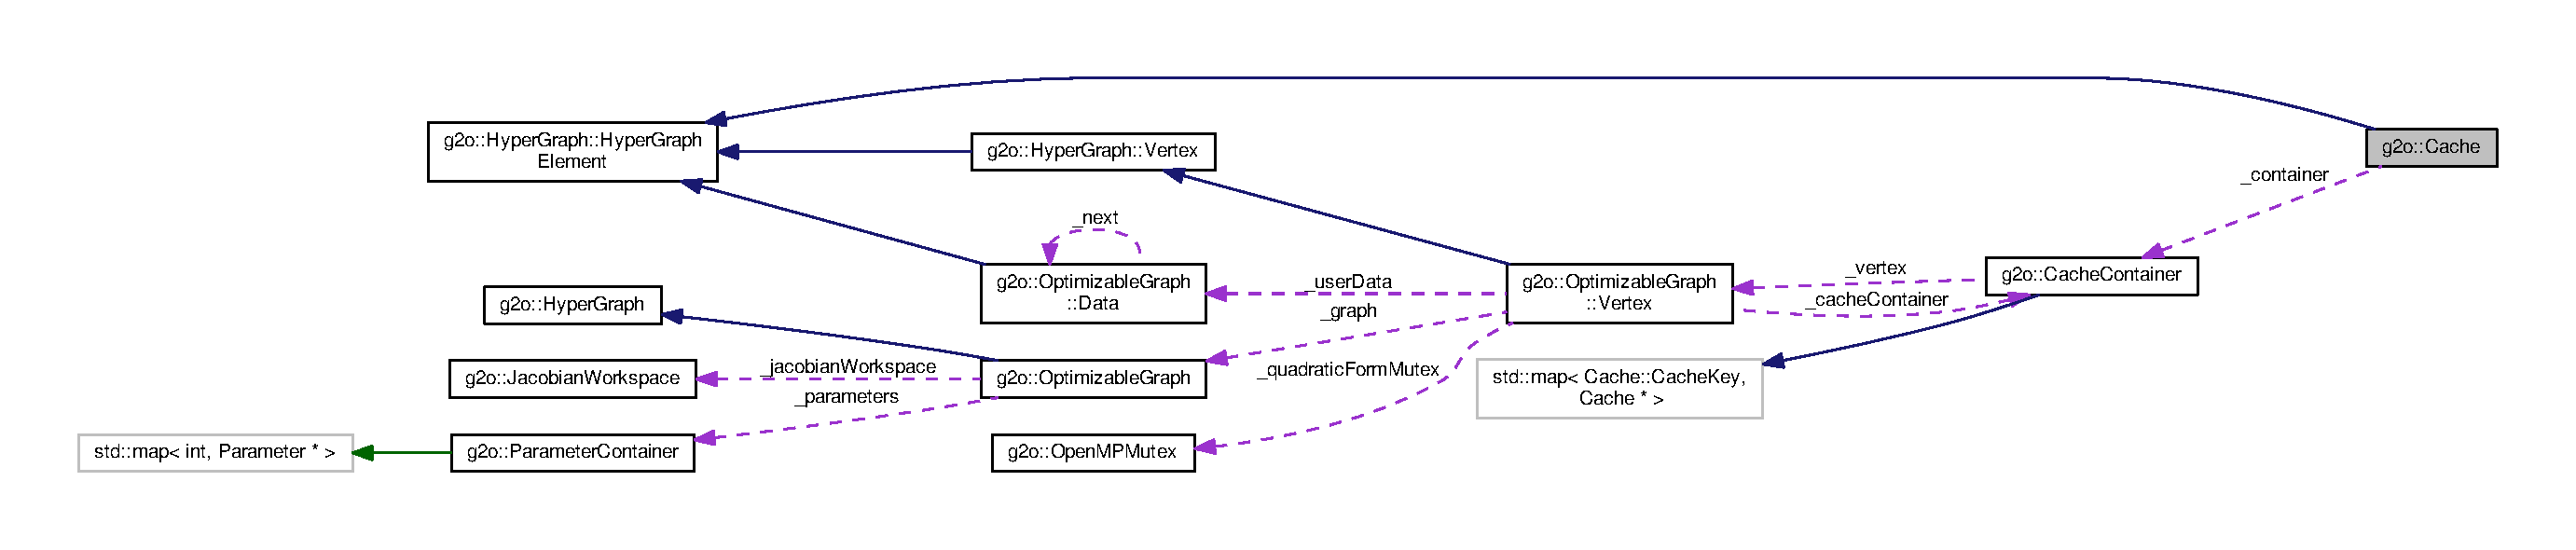
\includegraphics[width=350pt]{classg2o_1_1Cache__coll__graph}
\end{center}
\end{figure}
\subsection*{类}
\begin{DoxyCompactItemize}
\item 
class \hyperlink{classg2o_1_1Cache_1_1CacheKey}{Cache\-Key}
\end{DoxyCompactItemize}
\subsection*{Public 成员函数}
\begin{DoxyCompactItemize}
\item 
\hypertarget{classg2o_1_1Cache_adb5e57e9f06505511fdedb247a977cc3}{{\bfseries Cache} (\hyperlink{classg2o_1_1CacheContainer}{Cache\-Container} $\ast$container\-\_\-=0, const Parameter\-Vector \&parameters\-\_\-=Parameter\-Vector())}\label{classg2o_1_1Cache_adb5e57e9f06505511fdedb247a977cc3}

\item 
\hypertarget{classg2o_1_1Cache_a12c78ed261c8659c2539b6ebe52aea8f}{\hyperlink{classg2o_1_1Cache_1_1CacheKey}{Cache\-Key} {\bfseries key} () const }\label{classg2o_1_1Cache_a12c78ed261c8659c2539b6ebe52aea8f}

\item 
\hypertarget{classg2o_1_1Cache_ab94788e39d7e81201d14bc8ac58325c7}{\hyperlink{classg2o_1_1OptimizableGraph_1_1Vertex}{Optimizable\-Graph\-::\-Vertex} $\ast$ {\bfseries vertex} ()}\label{classg2o_1_1Cache_ab94788e39d7e81201d14bc8ac58325c7}

\item 
\hypertarget{classg2o_1_1Cache_a1a4480a445469d2d02b8db449e6cb57c}{\hyperlink{structg2o_1_1OptimizableGraph}{Optimizable\-Graph} $\ast$ {\bfseries graph} ()}\label{classg2o_1_1Cache_a1a4480a445469d2d02b8db449e6cb57c}

\item 
\hypertarget{classg2o_1_1Cache_a249ffa5c8ac120b3123bd151200082c9}{\hyperlink{classg2o_1_1CacheContainer}{Cache\-Container} $\ast$ {\bfseries container} ()}\label{classg2o_1_1Cache_a249ffa5c8ac120b3123bd151200082c9}

\item 
\hypertarget{classg2o_1_1Cache_a16e471be92f9fe24a3abdf11a0c546d2}{Parameter\-Vector \& {\bfseries parameters} ()}\label{classg2o_1_1Cache_a16e471be92f9fe24a3abdf11a0c546d2}

\item 
\hypertarget{classg2o_1_1Cache_aaea446a5eb59569acc67c94793975a0b}{void {\bfseries update} ()}\label{classg2o_1_1Cache_aaea446a5eb59569acc67c94793975a0b}

\item 
virtual \\*
Hyper\-Graph\-::\-Hyper\-Graph\-Element\-Type \hyperlink{classg2o_1_1Cache_a975c586e5a84dd3f4a85f364d5f92f91}{element\-Type} () const 
\end{DoxyCompactItemize}
\subsection*{Protected 成员函数}
\begin{DoxyCompactItemize}
\item 
\hypertarget{classg2o_1_1Cache_ae46e4a4e37c034925edd6bbfdfaa1cb2}{virtual void \hyperlink{classg2o_1_1Cache_ae46e4a4e37c034925edd6bbfdfaa1cb2}{update\-Impl} ()=0}\label{classg2o_1_1Cache_ae46e4a4e37c034925edd6bbfdfaa1cb2}

\begin{DoxyCompactList}\small\item\em redefine this to do the update \end{DoxyCompactList}\item 
\hyperlink{classg2o_1_1Cache}{Cache} $\ast$ \hyperlink{classg2o_1_1Cache_a776574fb98726ff61bc1280ea624c6e5}{install\-Dependency} (const std\-::string \&type\-\_\-, const std\-::vector$<$ int $>$ \&parameter\-Indices)
\item 
virtual bool \hyperlink{classg2o_1_1Cache_a0c26f0baa33a5902002f1ca2d5f57ece}{resolve\-Dependancies} ()
\end{DoxyCompactItemize}
\subsection*{Protected 属性}
\begin{DoxyCompactItemize}
\item 
\hypertarget{classg2o_1_1Cache_a28d0ad45da71d9b7bc6de4cf1fb0f9e4}{bool {\bfseries \-\_\-update\-Needed}}\label{classg2o_1_1Cache_a28d0ad45da71d9b7bc6de4cf1fb0f9e4}

\item 
\hypertarget{classg2o_1_1Cache_ad596a1a7591adece4664a43fc87b881d}{Parameter\-Vector {\bfseries \-\_\-parameters}}\label{classg2o_1_1Cache_ad596a1a7591adece4664a43fc87b881d}

\item 
\hypertarget{classg2o_1_1Cache_a0b38f0c773c02903acf8964f73c3aa26}{std\-::vector$<$ \hyperlink{classg2o_1_1Cache}{Cache} $\ast$ $>$ {\bfseries \-\_\-parent\-Caches}}\label{classg2o_1_1Cache_a0b38f0c773c02903acf8964f73c3aa26}

\item 
\hypertarget{classg2o_1_1Cache_a098aeecd7f0daa19a58f710ae7cb27c3}{\hyperlink{classg2o_1_1CacheContainer}{Cache\-Container} $\ast$ {\bfseries \-\_\-container}}\label{classg2o_1_1Cache_a098aeecd7f0daa19a58f710ae7cb27c3}

\end{DoxyCompactItemize}
\subsection*{友元}
\begin{DoxyCompactItemize}
\item 
\hypertarget{classg2o_1_1Cache_a86dec1e0424aa4ae4e6867c69efd7868}{class {\bfseries Cache\-Container}}\label{classg2o_1_1Cache_a86dec1e0424aa4ae4e6867c69efd7868}

\end{DoxyCompactItemize}


\subsection{详细描述}


在文件 cache.\-h 第 39 行定义.



\subsection{成员函数说明}
\hypertarget{classg2o_1_1Cache_a975c586e5a84dd3f4a85f364d5f92f91}{\index{g2o\-::\-Cache@{g2o\-::\-Cache}!element\-Type@{element\-Type}}
\index{element\-Type@{element\-Type}!g2o::Cache@{g2o\-::\-Cache}}
\subsubsection[{element\-Type}]{\setlength{\rightskip}{0pt plus 5cm}virtual Hyper\-Graph\-::\-Hyper\-Graph\-Element\-Type g2o\-::\-Cache\-::element\-Type (
\begin{DoxyParamCaption}
{}
\end{DoxyParamCaption}
) const\hspace{0.3cm}{\ttfamily [inline]}, {\ttfamily [virtual]}}}\label{classg2o_1_1Cache_a975c586e5a84dd3f4a85f364d5f92f91}
returns the type of the graph element, see Hyper\-Graph\-Element\-Type 

实现了 \hyperlink{structg2o_1_1HyperGraph_1_1HyperGraphElement_a1a9d7b748698c09d202373e06e413ef2}{g2o\-::\-Hyper\-Graph\-::\-Hyper\-Graph\-Element}.



在文件 cache.\-h 第 71 行定义.

\hypertarget{classg2o_1_1Cache_a776574fb98726ff61bc1280ea624c6e5}{\index{g2o\-::\-Cache@{g2o\-::\-Cache}!install\-Dependency@{install\-Dependency}}
\index{install\-Dependency@{install\-Dependency}!g2o::Cache@{g2o\-::\-Cache}}
\subsubsection[{install\-Dependency}]{\setlength{\rightskip}{0pt plus 5cm}{\bf Cache} $\ast$ g2o\-::\-Cache\-::install\-Dependency (
\begin{DoxyParamCaption}
\item[{const std\-::string \&}]{type\-\_\-, }
\item[{const std\-::vector$<$ int $>$ \&}]{parameter\-Indices}
\end{DoxyParamCaption}
)\hspace{0.3cm}{\ttfamily [protected]}}}\label{classg2o_1_1Cache_a776574fb98726ff61bc1280ea624c6e5}
this function installs and satisfies a cache 
\begin{DoxyParams}{参数}
{\em type\-\_\-} & the typename of the dependency \\
\hline
{\em parameter\-Indices} & a vector containing the indices if the parameters in \-\_\-parameters that will be used to assemble the Key of the cache being created For example if I have a cache of type C2, having parameters \char`\"{}\-A, B, and C\char`\"{}, and it depends on a cache of type C1 that depends on the parameters A and C, the parameter\-Indices should contain \char`\"{}0, 2\char`\"{}, since they are the positions in the parameter vector of C2 of the parameters needed to construct C1. \\
\hline
\end{DoxyParams}
\begin{DoxyReturn}{返回}
the newly created cache 
\end{DoxyReturn}


在文件 cache.\-cpp 第 95 行定义.

\hypertarget{classg2o_1_1Cache_a0c26f0baa33a5902002f1ca2d5f57ece}{\index{g2o\-::\-Cache@{g2o\-::\-Cache}!resolve\-Dependancies@{resolve\-Dependancies}}
\index{resolve\-Dependancies@{resolve\-Dependancies}!g2o::Cache@{g2o\-::\-Cache}}
\subsubsection[{resolve\-Dependancies}]{\setlength{\rightskip}{0pt plus 5cm}bool g2o\-::\-Cache\-::resolve\-Dependancies (
\begin{DoxyParamCaption}
{}
\end{DoxyParamCaption}
)\hspace{0.3cm}{\ttfamily [protected]}, {\ttfamily [virtual]}}}\label{classg2o_1_1Cache_a0c26f0baa33a5902002f1ca2d5f57ece}
Function to be called from a cache that has dependencies. It just invokes a sequence of \hyperlink{classg2o_1_1Cache_a776574fb98726ff61bc1280ea624c6e5}{install\-Dependency()}. Although the caches returned are stored in the \-\_\-parent\-Cache vector, it is better that you redefine your own cache member variables, for better readability 

在文件 cache.\-cpp 第 114 行定义.



该类的文档由以下文件生成\-:\begin{DoxyCompactItemize}
\item 
Thirdparty/g2o/g2o/core/cache.\-h\item 
Thirdparty/g2o/g2o/core/cache.\-cpp\end{DoxyCompactItemize}

\hypertarget{classg2o_1_1CacheContainer}{\section{g2o\-:\-:Cache\-Container类 参考}
\label{classg2o_1_1CacheContainer}\index{g2o\-::\-Cache\-Container@{g2o\-::\-Cache\-Container}}
}


类 g2o\-:\-:Cache\-Container 继承关系图\-:
\nopagebreak
\begin{figure}[H]
\begin{center}
\leavevmode
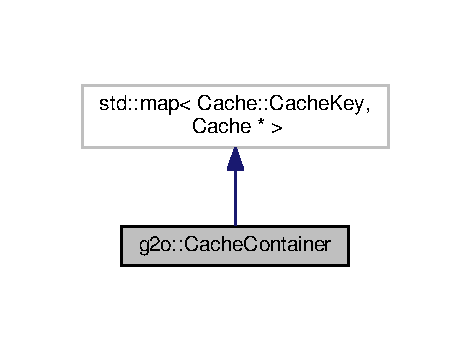
\includegraphics[width=226pt]{classg2o_1_1CacheContainer__inherit__graph}
\end{center}
\end{figure}


g2o\-:\-:Cache\-Container 的协作图\-:
\nopagebreak
\begin{figure}[H]
\begin{center}
\leavevmode
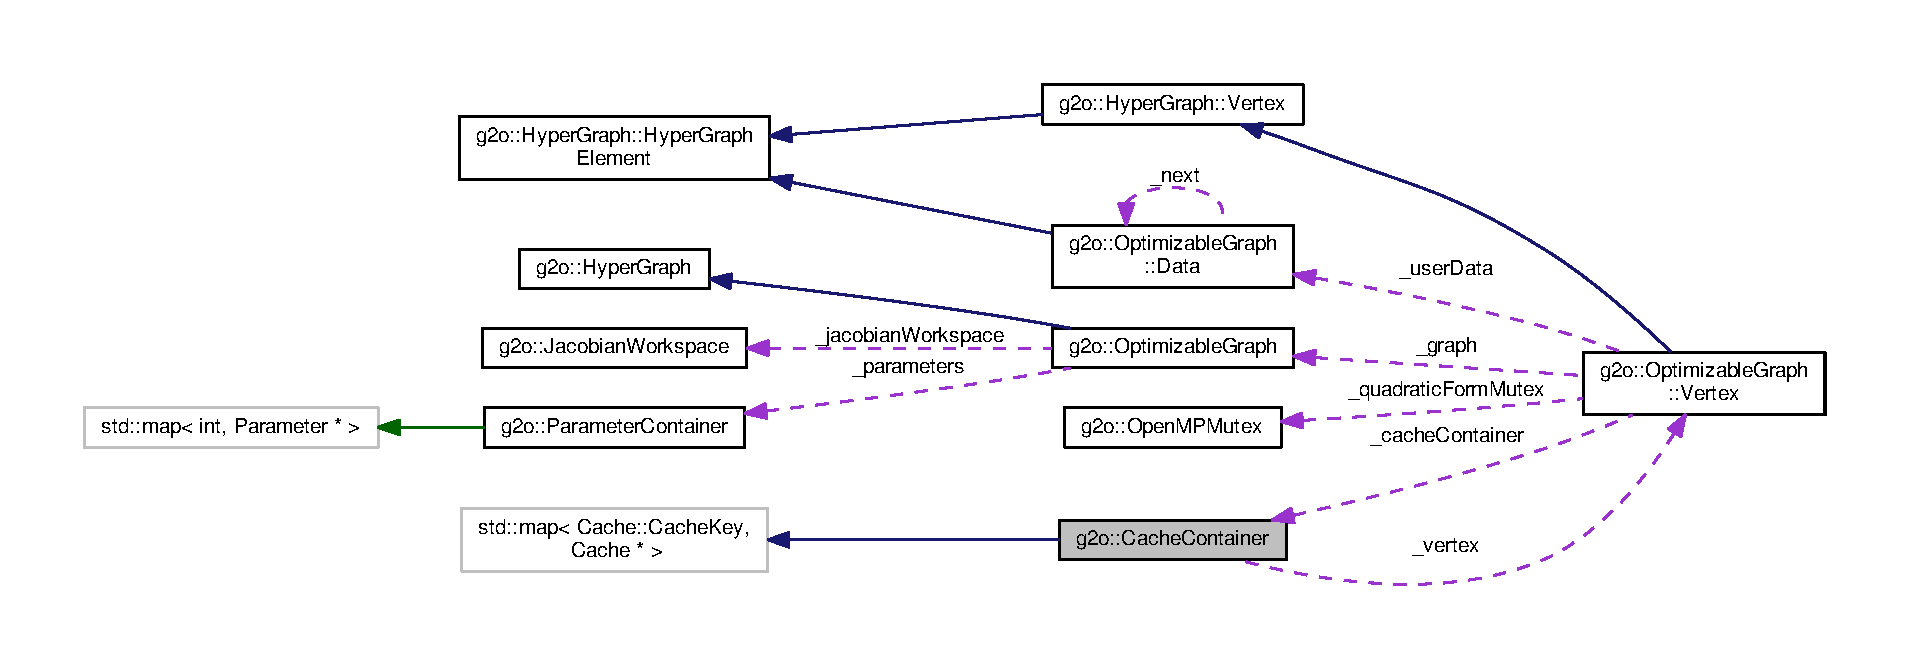
\includegraphics[width=350pt]{classg2o_1_1CacheContainer__coll__graph}
\end{center}
\end{figure}
\subsection*{Public 成员函数}
\begin{DoxyCompactItemize}
\item 
\hypertarget{classg2o_1_1CacheContainer_aed510932f7e499f2fd3c1fdea7809052}{{\bfseries Cache\-Container} (\hyperlink{classg2o_1_1OptimizableGraph_1_1Vertex}{Optimizable\-Graph\-::\-Vertex} $\ast$vertex\-\_\-)}\label{classg2o_1_1CacheContainer_aed510932f7e499f2fd3c1fdea7809052}

\item 
\hypertarget{classg2o_1_1CacheContainer_ada4f7f82992a85dbc742c1ab24c39c08}{\hyperlink{classg2o_1_1OptimizableGraph_1_1Vertex}{Optimizable\-Graph\-::\-Vertex} $\ast$ {\bfseries vertex} ()}\label{classg2o_1_1CacheContainer_ada4f7f82992a85dbc742c1ab24c39c08}

\item 
\hypertarget{classg2o_1_1CacheContainer_a4bf79d27bb9ae377446dfa7fd048b06d}{\hyperlink{structg2o_1_1OptimizableGraph}{Optimizable\-Graph} $\ast$ {\bfseries graph} ()}\label{classg2o_1_1CacheContainer_a4bf79d27bb9ae377446dfa7fd048b06d}

\item 
\hypertarget{classg2o_1_1CacheContainer_a2a0230117e0e71210f3d10a9e7143d0f}{\hyperlink{classg2o_1_1Cache}{Cache} $\ast$ {\bfseries find\-Cache} (const \hyperlink{classg2o_1_1Cache_1_1CacheKey}{Cache\-::\-Cache\-Key} \&key)}\label{classg2o_1_1CacheContainer_a2a0230117e0e71210f3d10a9e7143d0f}

\item 
\hypertarget{classg2o_1_1CacheContainer_a08902c228901e06c4e08c5b594683a6c}{\hyperlink{classg2o_1_1Cache}{Cache} $\ast$ {\bfseries create\-Cache} (const \hyperlink{classg2o_1_1Cache_1_1CacheKey}{Cache\-::\-Cache\-Key} \&key)}\label{classg2o_1_1CacheContainer_a08902c228901e06c4e08c5b594683a6c}

\item 
\hypertarget{classg2o_1_1CacheContainer_a2241f992e90c1078447553d0833ccf14}{void {\bfseries set\-Update\-Needed} (bool need\-Update=true)}\label{classg2o_1_1CacheContainer_a2241f992e90c1078447553d0833ccf14}

\item 
\hypertarget{classg2o_1_1CacheContainer_acc9a6d1fbc828f55b1a6af1c29f003df}{void {\bfseries update} ()}\label{classg2o_1_1CacheContainer_acc9a6d1fbc828f55b1a6af1c29f003df}

\end{DoxyCompactItemize}
\subsection*{Protected 属性}
\begin{DoxyCompactItemize}
\item 
\hypertarget{classg2o_1_1CacheContainer_a899b5f4d01859463cedf663b68f78391}{\hyperlink{classg2o_1_1OptimizableGraph_1_1Vertex}{Optimizable\-Graph\-::\-Vertex} $\ast$ {\bfseries \-\_\-vertex}}\label{classg2o_1_1CacheContainer_a899b5f4d01859463cedf663b68f78391}

\item 
\hypertarget{classg2o_1_1CacheContainer_a5fd5257863e41c3fc38336aaa7779b3e}{bool {\bfseries \-\_\-update\-Needed}}\label{classg2o_1_1CacheContainer_a5fd5257863e41c3fc38336aaa7779b3e}

\end{DoxyCompactItemize}


\subsection{详细描述}


在文件 cache.\-h 第 104 行定义.



该类的文档由以下文件生成\-:\begin{DoxyCompactItemize}
\item 
Thirdparty/g2o/g2o/core/cache.\-h\item 
Thirdparty/g2o/g2o/core/cache.\-cpp\end{DoxyCompactItemize}

\hypertarget{classg2o_1_1Cache_1_1CacheKey}{\section{g2o\-:\-:Cache\-:\-:Cache\-Key类 参考}
\label{classg2o_1_1Cache_1_1CacheKey}\index{g2o\-::\-Cache\-::\-Cache\-Key@{g2o\-::\-Cache\-::\-Cache\-Key}}
}
\subsection*{Public 成员函数}
\begin{DoxyCompactItemize}
\item 
\hypertarget{classg2o_1_1Cache_1_1CacheKey_a363ba06fe3b3f17acd664b0706ba3270}{{\bfseries Cache\-Key} (const std\-::string \&type\-\_\-, const Parameter\-Vector \&parameters\-\_\-)}\label{classg2o_1_1Cache_1_1CacheKey_a363ba06fe3b3f17acd664b0706ba3270}

\item 
\hypertarget{classg2o_1_1Cache_1_1CacheKey_a4a6e782eeee8c5300abe0fd5a89ed6a8}{bool {\bfseries operator$<$} (const \hyperlink{classg2o_1_1Cache_1_1CacheKey}{Cache\-Key} \&c) const }\label{classg2o_1_1Cache_1_1CacheKey_a4a6e782eeee8c5300abe0fd5a89ed6a8}

\item 
\hypertarget{classg2o_1_1Cache_1_1CacheKey_aea8a503e67d00d2376a5435c1d05be99}{const std\-::string \& {\bfseries type} () const }\label{classg2o_1_1Cache_1_1CacheKey_aea8a503e67d00d2376a5435c1d05be99}

\item 
\hypertarget{classg2o_1_1Cache_1_1CacheKey_ac872928298c0b413e152efd04e22cda6}{const Parameter\-Vector \& {\bfseries parameters} () const }\label{classg2o_1_1Cache_1_1CacheKey_ac872928298c0b413e152efd04e22cda6}

\end{DoxyCompactItemize}
\subsection*{Protected 属性}
\begin{DoxyCompactItemize}
\item 
\hypertarget{classg2o_1_1Cache_1_1CacheKey_a886ec6cf583561cb791cbaff902c673d}{std\-::string {\bfseries \-\_\-type}}\label{classg2o_1_1Cache_1_1CacheKey_a886ec6cf583561cb791cbaff902c673d}

\item 
\hypertarget{classg2o_1_1Cache_1_1CacheKey_a3f8dc2307bd1d174a30bdc8443a8d152}{Parameter\-Vector {\bfseries \-\_\-parameters}}\label{classg2o_1_1Cache_1_1CacheKey_a3f8dc2307bd1d174a30bdc8443a8d152}

\end{DoxyCompactItemize}
\subsection*{友元}
\begin{DoxyCompactItemize}
\item 
\hypertarget{classg2o_1_1Cache_1_1CacheKey_a86dec1e0424aa4ae4e6867c69efd7868}{class {\bfseries Cache\-Container}}\label{classg2o_1_1Cache_1_1CacheKey_a86dec1e0424aa4ae4e6867c69efd7868}

\end{DoxyCompactItemize}


\subsection{详细描述}


在文件 cache.\-h 第 43 行定义.



该类的文档由以下文件生成\-:\begin{DoxyCompactItemize}
\item 
Thirdparty/g2o/g2o/core/cache.\-h\item 
Thirdparty/g2o/g2o/core/cache.\-cpp\end{DoxyCompactItemize}

\hypertarget{classg2o_1_1LinearSolverEigen_1_1CholeskyDecomposition}{\section{g2o\-:\-:Linear\-Solver\-Eigen$<$ Matrix\-Type $>$\-:\-:Cholesky\-Decomposition类 参考}
\label{classg2o_1_1LinearSolverEigen_1_1CholeskyDecomposition}\index{g2o\-::\-Linear\-Solver\-Eigen$<$ Matrix\-Type $>$\-::\-Cholesky\-Decomposition@{g2o\-::\-Linear\-Solver\-Eigen$<$ Matrix\-Type $>$\-::\-Cholesky\-Decomposition}}
}


Sub-\/classing Eigen's Simplicial\-L\-D\-L\-T to perform ordering with a given ordering.  




{\ttfamily \#include $<$linear\-\_\-solver\-\_\-eigen.\-h$>$}



类 g2o\-:\-:Linear\-Solver\-Eigen$<$ Matrix\-Type $>$\-:\-:Cholesky\-Decomposition 继承关系图\-:
\nopagebreak
\begin{figure}[H]
\begin{center}
\leavevmode
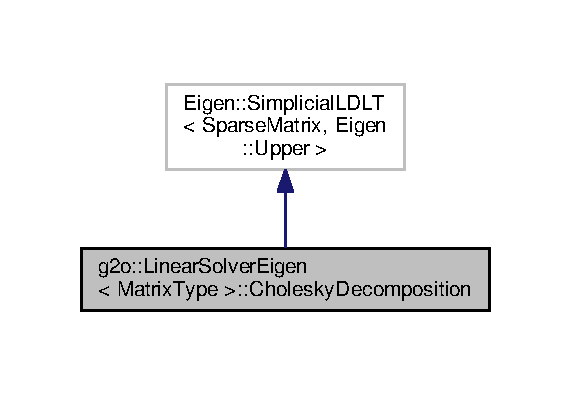
\includegraphics[width=274pt]{classg2o_1_1LinearSolverEigen_1_1CholeskyDecomposition__inherit__graph}
\end{center}
\end{figure}


g2o\-:\-:Linear\-Solver\-Eigen$<$ Matrix\-Type $>$\-:\-:Cholesky\-Decomposition 的协作图\-:
\nopagebreak
\begin{figure}[H]
\begin{center}
\leavevmode
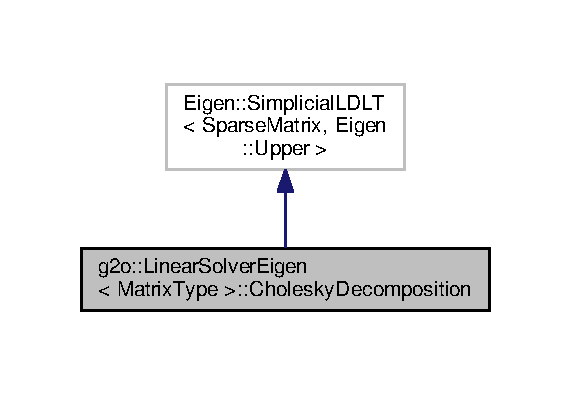
\includegraphics[width=274pt]{classg2o_1_1LinearSolverEigen_1_1CholeskyDecomposition__coll__graph}
\end{center}
\end{figure}
\subsection*{Public 成员函数}
\begin{DoxyCompactItemize}
\item 
\hypertarget{classg2o_1_1LinearSolverEigen_1_1CholeskyDecomposition_a3aa432f9aec0b7230c733df9a4d80558}{void {\bfseries analyze\-Pattern\-With\-Permutation} (Sparse\-Matrix \&a, const Permutation\-Matrix \&permutation)}\label{classg2o_1_1LinearSolverEigen_1_1CholeskyDecomposition_a3aa432f9aec0b7230c733df9a4d80558}

\end{DoxyCompactItemize}


\subsection{详细描述}
\subsubsection*{template$<$typename Matrix\-Type$>$class g2o\-::\-Linear\-Solver\-Eigen$<$ Matrix\-Type $>$\-::\-Cholesky\-Decomposition}

Sub-\/classing Eigen's Simplicial\-L\-D\-L\-T to perform ordering with a given ordering. 

在文件 linear\-\_\-solver\-\_\-eigen.\-h 第 60 行定义.



该类的文档由以下文件生成\-:\begin{DoxyCompactItemize}
\item 
Thirdparty/g2o/g2o/solvers/linear\-\_\-solver\-\_\-eigen.\-h\end{DoxyCompactItemize}

\hypertarget{structg2o_1_1ColSort}{\section{g2o\-:\-:Col\-Sort结构体 参考}
\label{structg2o_1_1ColSort}\index{g2o\-::\-Col\-Sort@{g2o\-::\-Col\-Sort}}
}
\subsection*{Public 成员函数}
\begin{DoxyCompactItemize}
\item 
\hypertarget{structg2o_1_1ColSort_a228d871d0007190ef880d303e56af609}{bool {\bfseries operator()} (const pair$<$ int, int $>$ \&e1, const pair$<$ int, int $>$ \&e2) const }\label{structg2o_1_1ColSort_a228d871d0007190ef880d303e56af609}

\end{DoxyCompactItemize}


\subsection{详细描述}


在文件 matrix\-\_\-structure.\-cpp 第 37 行定义.



该结构体的文档由以下文件生成\-:\begin{DoxyCompactItemize}
\item 
Thirdparty/g2o/g2o/core/matrix\-\_\-structure.\-cpp\end{DoxyCompactItemize}

\hypertarget{classORB__SLAM2_1_1Converter}{\section{O\-R\-B\-\_\-\-S\-L\-A\-M2\-:\-:Converter类 参考}
\label{classORB__SLAM2_1_1Converter}\index{O\-R\-B\-\_\-\-S\-L\-A\-M2\-::\-Converter@{O\-R\-B\-\_\-\-S\-L\-A\-M2\-::\-Converter}}
}


提供了一些常见的转换  




{\ttfamily \#include $<$Converter.\-h$>$}

\subsection*{静态 Public 成员函数}
\begin{DoxyCompactItemize}
\item 
\hypertarget{classORB__SLAM2_1_1Converter_abef47701eefdbc74c2c1625c140963fd}{static std\-::vector$<$ cv\-::\-Mat $>$ \hyperlink{classORB__SLAM2_1_1Converter_abef47701eefdbc74c2c1625c140963fd}{to\-Descriptor\-Vector} (const cv\-::\-Mat \&Descriptors)}\label{classORB__SLAM2_1_1Converter_abef47701eefdbc74c2c1625c140963fd}

\begin{DoxyCompactList}\small\item\em 一个描述子矩阵到一串单行的描述子向量 \end{DoxyCompactList}\end{DoxyCompactItemize}
\begin{Indent}{\bf to\-S\-E3\-Quat}\par
\begin{DoxyCompactItemize}
\item 
static \hyperlink{classg2o_1_1SE3Quat}{g2o\-::\-S\-E3\-Quat} \hyperlink{classORB__SLAM2_1_1Converter_a0b73791a3e2d90b4de41aed0ece2d0a2}{to\-S\-E3\-Quat} (const cv\-::\-Mat \&cv\-T)
\item 
static \hyperlink{classg2o_1_1SE3Quat}{g2o\-::\-S\-E3\-Quat} \hyperlink{classORB__SLAM2_1_1Converter_ac76ddd3b4d9a7e364e5cc72cfe483247}{to\-S\-E3\-Quat} (const \hyperlink{structg2o_1_1Sim3}{g2o\-::\-Sim3} \&g\-Sim3)
\end{DoxyCompactItemize}
\end{Indent}
\begin{Indent}{\bf to\-Cv\-Mat}\par
\begin{DoxyCompactItemize}
\item 
\hypertarget{classORB__SLAM2_1_1Converter_ac9d5a9ea7de26d34047aa0afddaa2091}{static cv\-::\-Mat {\bfseries to\-Cv\-Mat} (const \hyperlink{classg2o_1_1SE3Quat}{g2o\-::\-S\-E3\-Quat} \&S\-E3)}\label{classORB__SLAM2_1_1Converter_ac9d5a9ea7de26d34047aa0afddaa2091}

\item 
\hypertarget{classORB__SLAM2_1_1Converter_a4bc1702afbd33a5d90d39f1940157e08}{static cv\-::\-Mat {\bfseries to\-Cv\-Mat} (const \hyperlink{structg2o_1_1Sim3}{g2o\-::\-Sim3} \&Sim3)}\label{classORB__SLAM2_1_1Converter_a4bc1702afbd33a5d90d39f1940157e08}

\item 
\hypertarget{classORB__SLAM2_1_1Converter_a93055164116a8f35ecc5a9a5dcad1ca0}{static cv\-::\-Mat {\bfseries to\-Cv\-Mat} (const Eigen\-::\-Matrix$<$ double, 4, 4 $>$ \&m)}\label{classORB__SLAM2_1_1Converter_a93055164116a8f35ecc5a9a5dcad1ca0}

\item 
\hypertarget{classORB__SLAM2_1_1Converter_a7558c9fde7b818582bee8b4a4ff00793}{static cv\-::\-Mat {\bfseries to\-Cv\-Mat} (const Eigen\-::\-Matrix3d \&m)}\label{classORB__SLAM2_1_1Converter_a7558c9fde7b818582bee8b4a4ff00793}

\item 
\hypertarget{classORB__SLAM2_1_1Converter_a6748f1ecb782efc7741c1d2f6fbbed22}{static cv\-::\-Mat {\bfseries to\-Cv\-Mat} (const Eigen\-::\-Matrix$<$ double, 3, 1 $>$ \&m)}\label{classORB__SLAM2_1_1Converter_a6748f1ecb782efc7741c1d2f6fbbed22}

\item 
\hypertarget{classORB__SLAM2_1_1Converter_a0972ca8f56ea15c1814f51be3804978f}{static cv\-::\-Mat {\bfseries to\-Cv\-S\-E3} (const Eigen\-::\-Matrix$<$ double, 3, 3 $>$ \&R, const Eigen\-::\-Matrix$<$ double, 3, 1 $>$ \&t)}\label{classORB__SLAM2_1_1Converter_a0972ca8f56ea15c1814f51be3804978f}

\end{DoxyCompactItemize}
\end{Indent}
\begin{Indent}{\bf to\-Eigen}\par
\begin{DoxyCompactItemize}
\item 
\hypertarget{classORB__SLAM2_1_1Converter_a65fccab585e29d1acbf4c23e5ce69bdc}{static Eigen\-::\-Matrix$<$ double, 3, 1 $>$ {\bfseries to\-Vector3d} (const cv\-::\-Mat \&cv\-Vector)}\label{classORB__SLAM2_1_1Converter_a65fccab585e29d1acbf4c23e5ce69bdc}

\item 
\hypertarget{classORB__SLAM2_1_1Converter_af7b71b64b74fd45b39b9a7f47ee80145}{static Eigen\-::\-Matrix$<$ double, 3, 1 $>$ {\bfseries to\-Vector3d} (const cv\-::\-Point3f \&cv\-Point)}\label{classORB__SLAM2_1_1Converter_af7b71b64b74fd45b39b9a7f47ee80145}

\item 
\hypertarget{classORB__SLAM2_1_1Converter_a000a7971e46afdc95d6692a70006182b}{static Eigen\-::\-Matrix$<$ double, 3, 3 $>$ {\bfseries to\-Matrix3d} (const cv\-::\-Mat \&cv\-Mat3)}\label{classORB__SLAM2_1_1Converter_a000a7971e46afdc95d6692a70006182b}

\item 
\hypertarget{classORB__SLAM2_1_1Converter_a16b54bd921d9cdc83d289cfd1598fb3c}{static std\-::vector$<$ float $>$ {\bfseries to\-Quaternion} (const cv\-::\-Mat \&M)}\label{classORB__SLAM2_1_1Converter_a16b54bd921d9cdc83d289cfd1598fb3c}

\end{DoxyCompactItemize}
\end{Indent}


\subsection{详细描述}
提供了一些常见的转换 

orb中以cv\-::\-Mat为基本存储结构,到g2o和\-Eigen需要一个转换 这些转换都很简单,整个文件可以单独从orbslam里抽出来而不影响其他功能 

在文件 Converter.\-h 第 39 行定义.



\subsection{成员函数说明}
\hypertarget{classORB__SLAM2_1_1Converter_a0b73791a3e2d90b4de41aed0ece2d0a2}{\index{O\-R\-B\-\_\-\-S\-L\-A\-M2\-::\-Converter@{O\-R\-B\-\_\-\-S\-L\-A\-M2\-::\-Converter}!to\-S\-E3\-Quat@{to\-S\-E3\-Quat}}
\index{to\-S\-E3\-Quat@{to\-S\-E3\-Quat}!ORB_SLAM2::Converter@{O\-R\-B\-\_\-\-S\-L\-A\-M2\-::\-Converter}}
\subsubsection[{to\-S\-E3\-Quat}]{\setlength{\rightskip}{0pt plus 5cm}{\bf g2o\-::\-S\-E3\-Quat} O\-R\-B\-\_\-\-S\-L\-A\-M2\-::\-Converter\-::to\-S\-E3\-Quat (
\begin{DoxyParamCaption}
\item[{const cv\-::\-Mat \&}]{cv\-T}
\end{DoxyParamCaption}
)\hspace{0.3cm}{\ttfamily [static]}}}\label{classORB__SLAM2_1_1Converter_a0b73791a3e2d90b4de41aed0ece2d0a2}
cv\-::\-Mat to \hyperlink{classg2o_1_1SE3Quat}{g2o\-::\-S\-E3\-Quat} 

在文件 Converter.\-cpp 第 37 行定义.



参考自 O\-R\-B\-\_\-\-S\-L\-A\-M2\-::\-Optimizer\-::\-Bundle\-Adjustment(), O\-R\-B\-\_\-\-S\-L\-A\-M2\-::\-Optimizer\-::\-Local\-Bundle\-Adjustment() , 以及 O\-R\-B\-\_\-\-S\-L\-A\-M2\-::\-Optimizer\-::\-Pose\-Optimization().



这是这个函数的调用关系图\-:
\nopagebreak
\begin{figure}[H]
\begin{center}
\leavevmode
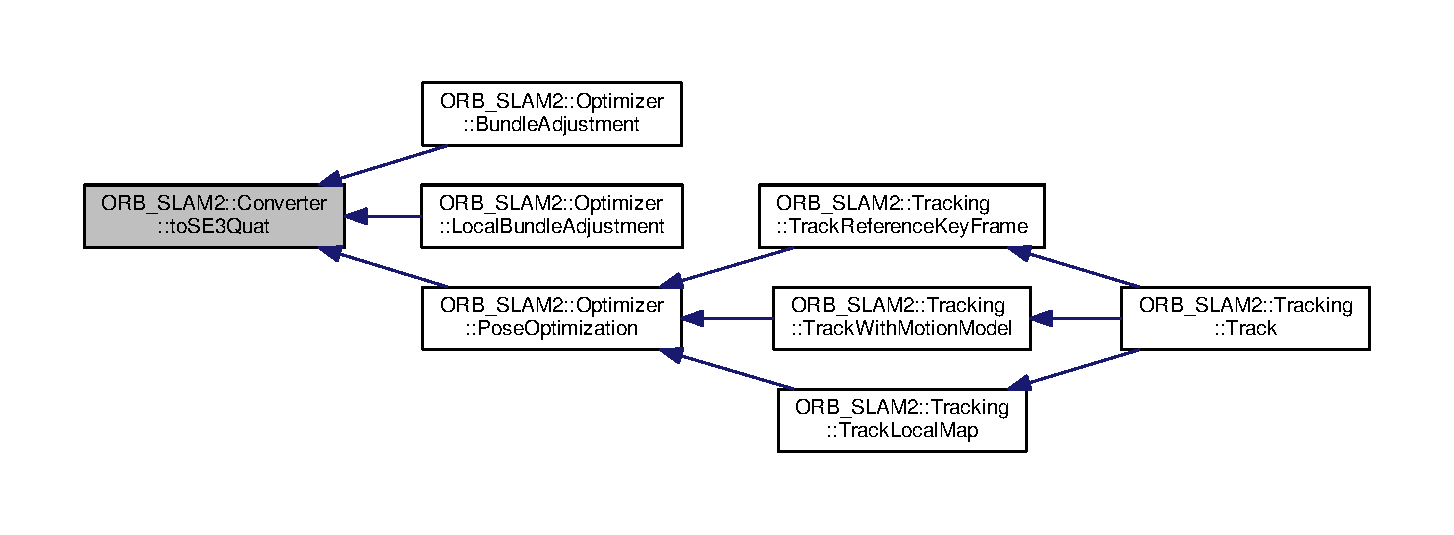
\includegraphics[width=350pt]{classORB__SLAM2_1_1Converter_a0b73791a3e2d90b4de41aed0ece2d0a2_icgraph}
\end{center}
\end{figure}


\hypertarget{classORB__SLAM2_1_1Converter_ac76ddd3b4d9a7e364e5cc72cfe483247}{\index{O\-R\-B\-\_\-\-S\-L\-A\-M2\-::\-Converter@{O\-R\-B\-\_\-\-S\-L\-A\-M2\-::\-Converter}!to\-S\-E3\-Quat@{to\-S\-E3\-Quat}}
\index{to\-S\-E3\-Quat@{to\-S\-E3\-Quat}!ORB_SLAM2::Converter@{O\-R\-B\-\_\-\-S\-L\-A\-M2\-::\-Converter}}
\subsubsection[{to\-S\-E3\-Quat}]{\setlength{\rightskip}{0pt plus 5cm}static {\bf g2o\-::\-S\-E3\-Quat} O\-R\-B\-\_\-\-S\-L\-A\-M2\-::\-Converter\-::to\-S\-E3\-Quat (
\begin{DoxyParamCaption}
\item[{const {\bf g2o\-::\-Sim3} \&}]{g\-Sim3}
\end{DoxyParamCaption}
)\hspace{0.3cm}{\ttfamily [static]}}}\label{classORB__SLAM2_1_1Converter_ac76ddd3b4d9a7e364e5cc72cfe483247}
unimplemented 

该类的文档由以下文件生成\-:\begin{DoxyCompactItemize}
\item 
include/Converter.\-h\item 
src/Converter.\-cpp\end{DoxyCompactItemize}

\hypertarget{structg2o_1_1HyperDijkstra_1_1CostFunction}{\section{g2o\-:\-:Hyper\-Dijkstra\-:\-:Cost\-Function结构体 参考}
\label{structg2o_1_1HyperDijkstra_1_1CostFunction}\index{g2o\-::\-Hyper\-Dijkstra\-::\-Cost\-Function@{g2o\-::\-Hyper\-Dijkstra\-::\-Cost\-Function}}
}


类 g2o\-:\-:Hyper\-Dijkstra\-:\-:Cost\-Function 继承关系图\-:
\nopagebreak
\begin{figure}[H]
\begin{center}
\leavevmode
\includegraphics[width=210pt]{structg2o_1_1HyperDijkstra_1_1CostFunction__inherit__graph}
\end{center}
\end{figure}
\subsection*{Public 成员函数}
\begin{DoxyCompactItemize}
\item 
\hypertarget{structg2o_1_1HyperDijkstra_1_1CostFunction_a6d30ca80400c75941851ae079cfd42fd}{virtual double {\bfseries operator()} (\hyperlink{classg2o_1_1HyperGraph_1_1Edge}{Hyper\-Graph\-::\-Edge} $\ast$e, \hyperlink{classg2o_1_1HyperGraph_1_1Vertex}{Hyper\-Graph\-::\-Vertex} $\ast$from, \hyperlink{classg2o_1_1HyperGraph_1_1Vertex}{Hyper\-Graph\-::\-Vertex} $\ast$to)=0}\label{structg2o_1_1HyperDijkstra_1_1CostFunction_a6d30ca80400c75941851ae079cfd42fd}

\end{DoxyCompactItemize}


\subsection{详细描述}


在文件 hyper\-\_\-dijkstra.\-h 第 40 行定义.



该结构体的文档由以下文件生成\-:\begin{DoxyCompactItemize}
\item 
Thirdparty/g2o/g2o/core/hyper\-\_\-dijkstra.\-h\end{DoxyCompactItemize}

\hypertarget{classg2o_1_1Factory_1_1CreatorInformation}{\section{g2o\-:\-:Factory\-:\-:Creator\-Information类 参考}
\label{classg2o_1_1Factory_1_1CreatorInformation}\index{g2o\-::\-Factory\-::\-Creator\-Information@{g2o\-::\-Factory\-::\-Creator\-Information}}
}


g2o\-:\-:Factory\-:\-:Creator\-Information 的协作图\-:
\nopagebreak
\begin{figure}[H]
\begin{center}
\leavevmode
\includegraphics[width=244pt]{classg2o_1_1Factory_1_1CreatorInformation__coll__graph}
\end{center}
\end{figure}
\subsection*{Public 属性}
\begin{DoxyCompactItemize}
\item 
\hypertarget{classg2o_1_1Factory_1_1CreatorInformation_a9fd5a1087992c17f869f1d59bc519c23}{\hyperlink{classg2o_1_1AbstractHyperGraphElementCreator}{Abstract\-Hyper\-Graph\-Element\-Creator} $\ast$ {\bfseries creator}}\label{classg2o_1_1Factory_1_1CreatorInformation_a9fd5a1087992c17f869f1d59bc519c23}

\item 
\hypertarget{classg2o_1_1Factory_1_1CreatorInformation_ab9fa4c8aec27d204f5ae6a7510c4e339}{int {\bfseries element\-Type\-Bit}}\label{classg2o_1_1Factory_1_1CreatorInformation_ab9fa4c8aec27d204f5ae6a7510c4e339}

\end{DoxyCompactItemize}


\subsection{详细描述}


在文件 factory.\-h 第 100 行定义.



该类的文档由以下文件生成\-:\begin{DoxyCompactItemize}
\item 
Thirdparty/g2o/g2o/core/factory.\-h\end{DoxyCompactItemize}

\hypertarget{classg2o_1_1OptimizableGraph_1_1Data}{\section{g2o\-:\-:Optimizable\-Graph\-:\-:Data类 参考}
\label{classg2o_1_1OptimizableGraph_1_1Data}\index{g2o\-::\-Optimizable\-Graph\-::\-Data@{g2o\-::\-Optimizable\-Graph\-::\-Data}}
}


data packet for a vertex. Extend this class to store in the vertices the potential additional information you need (e.\-g. images, laser scans, ...).  




{\ttfamily \#include $<$optimizable\-\_\-graph.\-h$>$}



类 g2o\-:\-:Optimizable\-Graph\-:\-:Data 继承关系图\-:
\nopagebreak
\begin{figure}[H]
\begin{center}
\leavevmode
\includegraphics[width=228pt]{classg2o_1_1OptimizableGraph_1_1Data__inherit__graph}
\end{center}
\end{figure}


g2o\-:\-:Optimizable\-Graph\-:\-:Data 的协作图\-:
\nopagebreak
\begin{figure}[H]
\begin{center}
\leavevmode
\includegraphics[width=258pt]{classg2o_1_1OptimizableGraph_1_1Data__coll__graph}
\end{center}
\end{figure}
\subsection*{Public 成员函数}
\begin{DoxyCompactItemize}
\item 
\hypertarget{classg2o_1_1OptimizableGraph_1_1Data_a4a206c86daba1b47425199befd2e1ed4}{virtual bool \hyperlink{classg2o_1_1OptimizableGraph_1_1Data_a4a206c86daba1b47425199befd2e1ed4}{read} (std\-::istream \&is)=0}\label{classg2o_1_1OptimizableGraph_1_1Data_a4a206c86daba1b47425199befd2e1ed4}

\begin{DoxyCompactList}\small\item\em read the data from a stream \end{DoxyCompactList}\item 
\hypertarget{classg2o_1_1OptimizableGraph_1_1Data_ad80cd8ea8013c54c766684ec0ef3daa3}{virtual bool \hyperlink{classg2o_1_1OptimizableGraph_1_1Data_ad80cd8ea8013c54c766684ec0ef3daa3}{write} (std\-::ostream \&os) const =0}\label{classg2o_1_1OptimizableGraph_1_1Data_ad80cd8ea8013c54c766684ec0ef3daa3}

\begin{DoxyCompactList}\small\item\em write the data to a stream \end{DoxyCompactList}\item 
virtual \\*
Hyper\-Graph\-::\-Hyper\-Graph\-Element\-Type \hyperlink{classg2o_1_1OptimizableGraph_1_1Data_aa549949b0bf442face4e3b06d1934706}{element\-Type} () const 
\item 
\hypertarget{classg2o_1_1OptimizableGraph_1_1Data_a7438fd566ec8b29680f13cffd2cf85f3}{const \hyperlink{classg2o_1_1OptimizableGraph_1_1Data}{Data} $\ast$ {\bfseries next} () const }\label{classg2o_1_1OptimizableGraph_1_1Data_a7438fd566ec8b29680f13cffd2cf85f3}

\item 
\hypertarget{classg2o_1_1OptimizableGraph_1_1Data_af9c0427357f1e81f9008c3173fddf34c}{\hyperlink{classg2o_1_1OptimizableGraph_1_1Data}{Data} $\ast$ {\bfseries next} ()}\label{classg2o_1_1OptimizableGraph_1_1Data_af9c0427357f1e81f9008c3173fddf34c}

\item 
\hypertarget{classg2o_1_1OptimizableGraph_1_1Data_a5811aac3f8eab3c19207663e946b343b}{void {\bfseries set\-Next} (\hyperlink{classg2o_1_1OptimizableGraph_1_1Data}{Data} $\ast$next\-\_\-)}\label{classg2o_1_1OptimizableGraph_1_1Data_a5811aac3f8eab3c19207663e946b343b}

\end{DoxyCompactItemize}
\subsection*{Protected 属性}
\begin{DoxyCompactItemize}
\item 
\hypertarget{classg2o_1_1OptimizableGraph_1_1Data_a8e0569f2b8cb8400d3eada1bd13c0ccb}{\hyperlink{classg2o_1_1OptimizableGraph_1_1Data}{Data} $\ast$ {\bfseries \-\_\-next}}\label{classg2o_1_1OptimizableGraph_1_1Data_a8e0569f2b8cb8400d3eada1bd13c0ccb}

\end{DoxyCompactItemize}
\subsection*{友元}
\begin{DoxyCompactItemize}
\item 
\hypertarget{classg2o_1_1OptimizableGraph_1_1Data_a45d35331ee3deca38c26d1efb6b961ae}{struct {\bfseries Optimizable\-Graph}}\label{classg2o_1_1OptimizableGraph_1_1Data_a45d35331ee3deca38c26d1efb6b961ae}

\end{DoxyCompactItemize}


\subsection{详细描述}
data packet for a vertex. Extend this class to store in the vertices the potential additional information you need (e.\-g. images, laser scans, ...). 

在文件 optimizable\-\_\-graph.\-h 第 82 行定义.



\subsection{成员函数说明}
\hypertarget{classg2o_1_1OptimizableGraph_1_1Data_aa549949b0bf442face4e3b06d1934706}{\index{g2o\-::\-Optimizable\-Graph\-::\-Data@{g2o\-::\-Optimizable\-Graph\-::\-Data}!element\-Type@{element\-Type}}
\index{element\-Type@{element\-Type}!g2o::OptimizableGraph::Data@{g2o\-::\-Optimizable\-Graph\-::\-Data}}
\subsubsection[{element\-Type}]{\setlength{\rightskip}{0pt plus 5cm}virtual Hyper\-Graph\-::\-Hyper\-Graph\-Element\-Type g2o\-::\-Optimizable\-Graph\-::\-Data\-::element\-Type (
\begin{DoxyParamCaption}
{}
\end{DoxyParamCaption}
) const\hspace{0.3cm}{\ttfamily [inline]}, {\ttfamily [virtual]}}}\label{classg2o_1_1OptimizableGraph_1_1Data_aa549949b0bf442face4e3b06d1934706}
returns the type of the graph element, see Hyper\-Graph\-Element\-Type 

实现了 \hyperlink{structg2o_1_1HyperGraph_1_1HyperGraphElement_a1a9d7b748698c09d202373e06e413ef2}{g2o\-::\-Hyper\-Graph\-::\-Hyper\-Graph\-Element}.



在文件 optimizable\-\_\-graph.\-h 第 92 行定义.



该类的文档由以下文件生成\-:\begin{DoxyCompactItemize}
\item 
Thirdparty/g2o/g2o/core/optimizable\-\_\-graph.\-h\item 
Thirdparty/g2o/g2o/core/optimizable\-\_\-graph.\-cpp\end{DoxyCompactItemize}

\hypertarget{classg2o_1_1DrawAction}{\section{g2o\-:\-:Draw\-Action类 参考}
\label{classg2o_1_1DrawAction}\index{g2o\-::\-Draw\-Action@{g2o\-::\-Draw\-Action}}
}


draw actions  




{\ttfamily \#include $<$hyper\-\_\-graph\-\_\-action.\-h$>$}



类 g2o\-:\-:Draw\-Action 继承关系图\-:
\nopagebreak
\begin{figure}[H]
\begin{center}
\leavevmode
\includegraphics[width=234pt]{classg2o_1_1DrawAction__inherit__graph}
\end{center}
\end{figure}


g2o\-:\-:Draw\-Action 的协作图\-:
\nopagebreak
\begin{figure}[H]
\begin{center}
\leavevmode
\includegraphics[width=350pt]{classg2o_1_1DrawAction__coll__graph}
\end{center}
\end{figure}
\subsection*{类}
\begin{DoxyCompactItemize}
\item 
class \hyperlink{classg2o_1_1DrawAction_1_1Parameters}{Parameters}
\end{DoxyCompactItemize}
\subsection*{Public 成员函数}
\begin{DoxyCompactItemize}
\item 
\hypertarget{classg2o_1_1DrawAction_a6b876d6a30fa564176dc6a3caefa572e}{{\bfseries Draw\-Action} (const std\-::string \&type\-Name\-\_\-)}\label{classg2o_1_1DrawAction_a6b876d6a30fa564176dc6a3caefa572e}

\end{DoxyCompactItemize}
\subsection*{Protected 成员函数}
\begin{DoxyCompactItemize}
\item 
\hypertarget{classg2o_1_1DrawAction_a9556cd6f8d1f842d45e046e1770699b0}{virtual bool {\bfseries refresh\-Property\-Ptrs} (\hyperlink{structg2o_1_1HyperGraphElementAction_1_1Parameters}{Hyper\-Graph\-Element\-Action\-::\-Parameters} $\ast$params\-\_\-)}\label{classg2o_1_1DrawAction_a9556cd6f8d1f842d45e046e1770699b0}

\end{DoxyCompactItemize}
\subsection*{Protected 属性}
\begin{DoxyCompactItemize}
\item 
\hypertarget{classg2o_1_1DrawAction_af598eb77ea4e27a1c0a27533c971639d}{\hyperlink{classg2o_1_1DrawAction_1_1Parameters}{Parameters} $\ast$ {\bfseries \-\_\-previous\-Params}}\label{classg2o_1_1DrawAction_af598eb77ea4e27a1c0a27533c971639d}

\item 
\hypertarget{classg2o_1_1DrawAction_a1ec3a46473daeb8ac65e6a523a9248b6}{\hyperlink{classg2o_1_1Property}{Bool\-Property} $\ast$ {\bfseries \-\_\-show}}\label{classg2o_1_1DrawAction_a1ec3a46473daeb8ac65e6a523a9248b6}

\item 
\hypertarget{classg2o_1_1DrawAction_ab5f870bf2a931e64bc994c87c4212ad3}{\hyperlink{classg2o_1_1Property}{Bool\-Property} $\ast$ {\bfseries \-\_\-show\-Id}}\label{classg2o_1_1DrawAction_ab5f870bf2a931e64bc994c87c4212ad3}

\end{DoxyCompactItemize}
\subsection*{额外继承的成员函数}


\subsection{详细描述}
draw actions 

在文件 hyper\-\_\-graph\-\_\-action.\-h 第 179 行定义.



该类的文档由以下文件生成\-:\begin{DoxyCompactItemize}
\item 
Thirdparty/g2o/g2o/core/hyper\-\_\-graph\-\_\-action.\-h\item 
Thirdparty/g2o/g2o/core/hyper\-\_\-graph\-\_\-action.\-cpp\end{DoxyCompactItemize}

\hypertarget{classg2o_1_1HyperGraph_1_1Edge}{\section{g2o\-:\-:Hyper\-Graph\-:\-:Edge类 参考}
\label{classg2o_1_1HyperGraph_1_1Edge}\index{g2o\-::\-Hyper\-Graph\-::\-Edge@{g2o\-::\-Hyper\-Graph\-::\-Edge}}
}


{\ttfamily \#include $<$hyper\-\_\-graph.\-h$>$}



类 g2o\-:\-:Hyper\-Graph\-:\-:Edge 继承关系图\-:
\nopagebreak
\begin{figure}[H]
\begin{center}
\leavevmode
\includegraphics[width=350pt]{classg2o_1_1HyperGraph_1_1Edge__inherit__graph}
\end{center}
\end{figure}


g2o\-:\-:Hyper\-Graph\-:\-:Edge 的协作图\-:
\nopagebreak
\begin{figure}[H]
\begin{center}
\leavevmode
\includegraphics[width=228pt]{classg2o_1_1HyperGraph_1_1Edge__coll__graph}
\end{center}
\end{figure}
\subsection*{Public 成员函数}
\begin{DoxyCompactItemize}
\item 
\hypertarget{classg2o_1_1HyperGraph_1_1Edge_a891618b34652837ef0bee7084db81f2e}{\hyperlink{classg2o_1_1HyperGraph_1_1Edge_a891618b34652837ef0bee7084db81f2e}{Edge} (int id=-\/1)}\label{classg2o_1_1HyperGraph_1_1Edge_a891618b34652837ef0bee7084db81f2e}

\begin{DoxyCompactList}\small\item\em creates and empty edge with no vertices \end{DoxyCompactList}\item 
virtual void \hyperlink{classg2o_1_1HyperGraph_1_1Edge_ad8913f1149a0fd5bb628f0f1c8a91a55}{resize} (size\-\_\-t size)
\item 
const Vertex\-Container \& \hyperlink{classg2o_1_1HyperGraph_1_1Edge_a6410bb70a917b5407770ef1f1090b5f5}{vertices} () const 
\item 
Vertex\-Container \& \hyperlink{classg2o_1_1HyperGraph_1_1Edge_a67d1c5cb557deab9e9e361c63359fe60}{vertices} ()
\item 
const \hyperlink{classg2o_1_1HyperGraph_1_1Vertex}{Vertex} $\ast$ \hyperlink{classg2o_1_1HyperGraph_1_1Edge_aaec0b2c92c5496d0f0fea8f1abdc4311}{vertex} (size\-\_\-t i) const 
\item 
\hyperlink{classg2o_1_1HyperGraph_1_1Vertex}{Vertex} $\ast$ \hyperlink{classg2o_1_1HyperGraph_1_1Edge_af544d5d17d900c5aa2b5c9219d8e716f}{vertex} (size\-\_\-t i)
\item 
void \hyperlink{classg2o_1_1HyperGraph_1_1Edge_a5e957658d6e65c49b81197d052a7f16f}{set\-Vertex} (size\-\_\-t i, \hyperlink{classg2o_1_1HyperGraph_1_1Vertex}{Vertex} $\ast$v)
\item 
\hypertarget{classg2o_1_1HyperGraph_1_1Edge_a397a7fb12379b2c48b5e6bc4c6c71fc0}{int {\bfseries id} () const }\label{classg2o_1_1HyperGraph_1_1Edge_a397a7fb12379b2c48b5e6bc4c6c71fc0}

\item 
\hypertarget{classg2o_1_1HyperGraph_1_1Edge_a1270ed91efa5f7a0fc42229356cc23e1}{void {\bfseries set\-Id} (int id)}\label{classg2o_1_1HyperGraph_1_1Edge_a1270ed91efa5f7a0fc42229356cc23e1}

\item 
virtual Hyper\-Graph\-Element\-Type \hyperlink{classg2o_1_1HyperGraph_1_1Edge_a73df6169b3669d48f86eef90de0fcc26}{element\-Type} () const 
\end{DoxyCompactItemize}
\subsection*{Protected 属性}
\begin{DoxyCompactItemize}
\item 
\hypertarget{classg2o_1_1HyperGraph_1_1Edge_aabb036d331fc7f2524ec8611b638de92}{Vertex\-Container {\bfseries \-\_\-vertices}}\label{classg2o_1_1HyperGraph_1_1Edge_aabb036d331fc7f2524ec8611b638de92}

\item 
\hypertarget{classg2o_1_1HyperGraph_1_1Edge_aa1b6978624f7c165a4e0461cb5ff18fa}{int \hyperlink{classg2o_1_1HyperGraph_1_1Edge_aa1b6978624f7c165a4e0461cb5ff18fa}{\-\_\-id}}\label{classg2o_1_1HyperGraph_1_1Edge_aa1b6978624f7c165a4e0461cb5ff18fa}

\begin{DoxyCompactList}\small\item\em unique id \end{DoxyCompactList}\end{DoxyCompactItemize}


\subsection{详细描述}
Abstract \hyperlink{classg2o_1_1HyperGraph_1_1Edge}{Edge} class. Your nice edge classes should inherit from that one. An hyper-\/edge has pointers to the vertices it connects and stores them in a vector. 

在文件 hyper\-\_\-graph.\-h 第 124 行定义.



\subsection{成员函数说明}
\hypertarget{classg2o_1_1HyperGraph_1_1Edge_a73df6169b3669d48f86eef90de0fcc26}{\index{g2o\-::\-Hyper\-Graph\-::\-Edge@{g2o\-::\-Hyper\-Graph\-::\-Edge}!element\-Type@{element\-Type}}
\index{element\-Type@{element\-Type}!g2o::HyperGraph::Edge@{g2o\-::\-Hyper\-Graph\-::\-Edge}}
\subsubsection[{element\-Type}]{\setlength{\rightskip}{0pt plus 5cm}virtual Hyper\-Graph\-Element\-Type g2o\-::\-Hyper\-Graph\-::\-Edge\-::element\-Type (
\begin{DoxyParamCaption}
{}
\end{DoxyParamCaption}
) const\hspace{0.3cm}{\ttfamily [inline]}, {\ttfamily [virtual]}}}\label{classg2o_1_1HyperGraph_1_1Edge_a73df6169b3669d48f86eef90de0fcc26}
returns the type of the graph element, see Hyper\-Graph\-Element\-Type 

实现了 \hyperlink{structg2o_1_1HyperGraph_1_1HyperGraphElement_a1a9d7b748698c09d202373e06e413ef2}{g2o\-::\-Hyper\-Graph\-::\-Hyper\-Graph\-Element}.



在文件 hyper\-\_\-graph.\-h 第 157 行定义.

\hypertarget{classg2o_1_1HyperGraph_1_1Edge_ad8913f1149a0fd5bb628f0f1c8a91a55}{\index{g2o\-::\-Hyper\-Graph\-::\-Edge@{g2o\-::\-Hyper\-Graph\-::\-Edge}!resize@{resize}}
\index{resize@{resize}!g2o::HyperGraph::Edge@{g2o\-::\-Hyper\-Graph\-::\-Edge}}
\subsubsection[{resize}]{\setlength{\rightskip}{0pt plus 5cm}void g2o\-::\-Hyper\-Graph\-::\-Edge\-::resize (
\begin{DoxyParamCaption}
\item[{size\-\_\-t}]{size}
\end{DoxyParamCaption}
)\hspace{0.3cm}{\ttfamily [virtual]}}}\label{classg2o_1_1HyperGraph_1_1Edge_ad8913f1149a0fd5bb628f0f1c8a91a55}
resizes the number of vertices connected by this edge 

被 \hyperlink{classg2o_1_1BaseMultiEdge_ae07ec9359cd515d0abc2100ee8aae93f}{g2o\-::\-Base\-Multi\-Edge$<$ D, E $>$}, \hyperlink{classg2o_1_1BaseBinaryEdge_a06e64067fa5fff4a5e2d058249b55478}{g2o\-::\-Base\-Binary\-Edge$<$ D, E, Vertex\-Xi, Vertex\-Xj $>$}, \hyperlink{classg2o_1_1BaseBinaryEdge_a06e64067fa5fff4a5e2d058249b55478}{g2o\-::\-Base\-Binary\-Edge$<$ 2, Vector2d, Vertex\-S\-B\-A\-Point\-X\-Y\-Z, Vertex\-Sim3\-Expmap $>$}, \hyperlink{classg2o_1_1BaseBinaryEdge_a06e64067fa5fff4a5e2d058249b55478}{g2o\-::\-Base\-Binary\-Edge$<$ 7, Sim3, Vertex\-Sim3\-Expmap, Vertex\-Sim3\-Expmap $>$}, \hyperlink{classg2o_1_1BaseBinaryEdge_a06e64067fa5fff4a5e2d058249b55478}{g2o\-::\-Base\-Binary\-Edge$<$ 2, Vector2d, Vertex\-S\-B\-A\-Point\-X\-Y\-Z, Vertex\-S\-E3\-Expmap $>$}, \hyperlink{classg2o_1_1BaseBinaryEdge_a06e64067fa5fff4a5e2d058249b55478}{g2o\-::\-Base\-Binary\-Edge$<$ 3, Vector3d, Vertex\-S\-B\-A\-Point\-X\-Y\-Z, Vertex\-S\-E3\-Expmap $>$}, \hyperlink{classg2o_1_1BaseUnaryEdge_a01fcdfd2d3ed0325655bb99db95c0b10}{g2o\-::\-Base\-Unary\-Edge$<$ D, E, Vertex\-Xi $>$}, \hyperlink{classg2o_1_1BaseUnaryEdge_a01fcdfd2d3ed0325655bb99db95c0b10}{g2o\-::\-Base\-Unary\-Edge$<$ 2, Vector2d, Vertex\-S\-E3\-Expmap $>$} , 以及 \hyperlink{classg2o_1_1BaseUnaryEdge_a01fcdfd2d3ed0325655bb99db95c0b10}{g2o\-::\-Base\-Unary\-Edge$<$ 3, Vector3d, Vertex\-S\-E3\-Expmap $>$} 重载.



在文件 hyper\-\_\-graph.\-cpp 第 50 行定义.



参考自 g2o\-::\-Optimizable\-Graph\-::add\-Graph(), g2o\-::\-Base\-Unary\-Edge$<$ D, E, Vertex\-Xi $>$\-::construct\-Quadratic\-Form() , 以及 g2o\-::\-Base\-Binary\-Edge$<$ D, E, Vertex\-Xi, Vertex\-Xj $>$\-::construct\-Quadratic\-Form().



这是这个函数的调用关系图\-:
\nopagebreak
\begin{figure}[H]
\begin{center}
\leavevmode
\includegraphics[width=350pt]{classg2o_1_1HyperGraph_1_1Edge_ad8913f1149a0fd5bb628f0f1c8a91a55_icgraph}
\end{center}
\end{figure}


\hypertarget{classg2o_1_1HyperGraph_1_1Edge_a5e957658d6e65c49b81197d052a7f16f}{\index{g2o\-::\-Hyper\-Graph\-::\-Edge@{g2o\-::\-Hyper\-Graph\-::\-Edge}!set\-Vertex@{set\-Vertex}}
\index{set\-Vertex@{set\-Vertex}!g2o::HyperGraph::Edge@{g2o\-::\-Hyper\-Graph\-::\-Edge}}
\subsubsection[{set\-Vertex}]{\setlength{\rightskip}{0pt plus 5cm}void g2o\-::\-Hyper\-Graph\-::\-Edge\-::set\-Vertex (
\begin{DoxyParamCaption}
\item[{size\-\_\-t}]{i, }
\item[{{\bf Vertex} $\ast$}]{v}
\end{DoxyParamCaption}
)\hspace{0.3cm}{\ttfamily [inline]}}}\label{classg2o_1_1HyperGraph_1_1Edge_a5e957658d6e65c49b81197d052a7f16f}
set the ith vertex on the hyper-\/edge to the pointer supplied 

在文件 hyper\-\_\-graph.\-h 第 153 行定义.



参考自 g2o\-::\-Optimizable\-Graph\-::add\-Graph(), O\-R\-B\-\_\-\-S\-L\-A\-M2\-::\-Optimizer\-::\-Bundle\-Adjustment(), O\-R\-B\-\_\-\-S\-L\-A\-M2\-::\-Optimizer\-::\-Local\-Bundle\-Adjustment(), O\-R\-B\-\_\-\-S\-L\-A\-M2\-::\-Optimizer\-::\-Optimize\-Essential\-Graph(), O\-R\-B\-\_\-\-S\-L\-A\-M2\-::\-Optimizer\-::\-Optimize\-Sim3() , 以及 O\-R\-B\-\_\-\-S\-L\-A\-M2\-::\-Optimizer\-::\-Pose\-Optimization().



这是这个函数的调用关系图\-:
\nopagebreak
\begin{figure}[H]
\begin{center}
\leavevmode
\includegraphics[width=350pt]{classg2o_1_1HyperGraph_1_1Edge_a5e957658d6e65c49b81197d052a7f16f_icgraph}
\end{center}
\end{figure}


\hypertarget{classg2o_1_1HyperGraph_1_1Edge_aaec0b2c92c5496d0f0fea8f1abdc4311}{\index{g2o\-::\-Hyper\-Graph\-::\-Edge@{g2o\-::\-Hyper\-Graph\-::\-Edge}!vertex@{vertex}}
\index{vertex@{vertex}!g2o::HyperGraph::Edge@{g2o\-::\-Hyper\-Graph\-::\-Edge}}
\subsubsection[{vertex}]{\setlength{\rightskip}{0pt plus 5cm}const {\bf Vertex}$\ast$ g2o\-::\-Hyper\-Graph\-::\-Edge\-::vertex (
\begin{DoxyParamCaption}
\item[{size\-\_\-t}]{i}
\end{DoxyParamCaption}
) const\hspace{0.3cm}{\ttfamily [inline]}}}\label{classg2o_1_1HyperGraph_1_1Edge_aaec0b2c92c5496d0f0fea8f1abdc4311}
returns the pointer to the ith vertex connected to the hyper-\/edge. 

在文件 hyper\-\_\-graph.\-h 第 145 行定义.



参考自 g2o\-::\-Block\-Solver$<$ Traits $>$\-::build\-Structure(), g2o\-::\-Block\-Solver$<$ Traits $>$\-::build\-System(), g2o\-::\-Sparse\-Optimizer\-::compute\-Initial\-Guess(), g2o\-::\-Estimate\-Propagator\-::propagate(), g2o\-::\-Jacobian\-Workspace\-::update\-Size(), g2o\-::\-Block\-Solver$<$ Traits $>$\-::update\-Structure() , 以及 g2o\-::\-Optimizable\-Graph\-::verify\-Information\-Matrices().



这是这个函数的调用关系图\-:
\nopagebreak
\begin{figure}[H]
\begin{center}
\leavevmode
\includegraphics[width=350pt]{classg2o_1_1HyperGraph_1_1Edge_aaec0b2c92c5496d0f0fea8f1abdc4311_icgraph}
\end{center}
\end{figure}


\hypertarget{classg2o_1_1HyperGraph_1_1Edge_af544d5d17d900c5aa2b5c9219d8e716f}{\index{g2o\-::\-Hyper\-Graph\-::\-Edge@{g2o\-::\-Hyper\-Graph\-::\-Edge}!vertex@{vertex}}
\index{vertex@{vertex}!g2o::HyperGraph::Edge@{g2o\-::\-Hyper\-Graph\-::\-Edge}}
\subsubsection[{vertex}]{\setlength{\rightskip}{0pt plus 5cm}{\bf Vertex}$\ast$ g2o\-::\-Hyper\-Graph\-::\-Edge\-::vertex (
\begin{DoxyParamCaption}
\item[{size\-\_\-t}]{i}
\end{DoxyParamCaption}
)\hspace{0.3cm}{\ttfamily [inline]}}}\label{classg2o_1_1HyperGraph_1_1Edge_af544d5d17d900c5aa2b5c9219d8e716f}
returns the pointer to the ith vertex connected to the hyper-\/edge. 

在文件 hyper\-\_\-graph.\-h 第 149 行定义.

\hypertarget{classg2o_1_1HyperGraph_1_1Edge_a6410bb70a917b5407770ef1f1090b5f5}{\index{g2o\-::\-Hyper\-Graph\-::\-Edge@{g2o\-::\-Hyper\-Graph\-::\-Edge}!vertices@{vertices}}
\index{vertices@{vertices}!g2o::HyperGraph::Edge@{g2o\-::\-Hyper\-Graph\-::\-Edge}}
\subsubsection[{vertices}]{\setlength{\rightskip}{0pt plus 5cm}const Vertex\-Container\& g2o\-::\-Hyper\-Graph\-::\-Edge\-::vertices (
\begin{DoxyParamCaption}
{}
\end{DoxyParamCaption}
) const\hspace{0.3cm}{\ttfamily [inline]}}}\label{classg2o_1_1HyperGraph_1_1Edge_a6410bb70a917b5407770ef1f1090b5f5}
returns the vector of pointers to the vertices connected by the hyper-\/edge. 

在文件 hyper\-\_\-graph.\-h 第 137 行定义.



参考自 g2o\-::\-Hyper\-Graph\-::add\-Edge(), g2o\-::\-Optimizable\-Graph\-::add\-Graph(), g2o\-::\-Block\-Solver$<$ Traits $>$\-::build\-Structure(), g2o\-::\-Block\-Solver$<$ Traits $>$\-::build\-System(), g2o\-::\-Sparse\-Optimizer\-::compute\-Initial\-Guess(), g2o\-::\-Sparse\-Optimizer\-::initialize\-Optimization(), g2o\-::\-Estimate\-Propagator\-::propagate(), g2o\-::\-Hyper\-Graph\-::remove\-Edge(), g2o\-::\-Jacobian\-Workspace\-::update\-Size(), g2o\-::\-Block\-Solver$<$ Traits $>$\-::update\-Structure() , 以及 g2o\-::\-Optimizable\-Graph\-::verify\-Information\-Matrices().



这是这个函数的调用关系图\-:
\nopagebreak
\begin{figure}[H]
\begin{center}
\leavevmode
\includegraphics[width=350pt]{classg2o_1_1HyperGraph_1_1Edge_a6410bb70a917b5407770ef1f1090b5f5_icgraph}
\end{center}
\end{figure}


\hypertarget{classg2o_1_1HyperGraph_1_1Edge_a67d1c5cb557deab9e9e361c63359fe60}{\index{g2o\-::\-Hyper\-Graph\-::\-Edge@{g2o\-::\-Hyper\-Graph\-::\-Edge}!vertices@{vertices}}
\index{vertices@{vertices}!g2o::HyperGraph::Edge@{g2o\-::\-Hyper\-Graph\-::\-Edge}}
\subsubsection[{vertices}]{\setlength{\rightskip}{0pt plus 5cm}Vertex\-Container\& g2o\-::\-Hyper\-Graph\-::\-Edge\-::vertices (
\begin{DoxyParamCaption}
{}
\end{DoxyParamCaption}
)\hspace{0.3cm}{\ttfamily [inline]}}}\label{classg2o_1_1HyperGraph_1_1Edge_a67d1c5cb557deab9e9e361c63359fe60}
returns the vector of pointers to the vertices connected by the hyper-\/edge. 

在文件 hyper\-\_\-graph.\-h 第 141 行定义.



该类的文档由以下文件生成\-:\begin{DoxyCompactItemize}
\item 
Thirdparty/g2o/g2o/core/hyper\-\_\-graph.\-h\item 
Thirdparty/g2o/g2o/core/hyper\-\_\-graph.\-cpp\end{DoxyCompactItemize}

\hypertarget{classg2o_1_1OptimizableGraph_1_1Edge}{\section{g2o\-:\-:Optimizable\-Graph\-:\-:Edge类 参考}
\label{classg2o_1_1OptimizableGraph_1_1Edge}\index{g2o\-::\-Optimizable\-Graph\-::\-Edge@{g2o\-::\-Optimizable\-Graph\-::\-Edge}}
}


类 g2o\-:\-:Optimizable\-Graph\-:\-:Edge 继承关系图\-:
\nopagebreak
\begin{figure}[H]
\begin{center}
\leavevmode
\includegraphics[width=350pt]{classg2o_1_1OptimizableGraph_1_1Edge__inherit__graph}
\end{center}
\end{figure}


g2o\-:\-:Optimizable\-Graph\-:\-:Edge 的协作图\-:
\nopagebreak
\begin{figure}[H]
\begin{center}
\leavevmode
\includegraphics[width=333pt]{classg2o_1_1OptimizableGraph_1_1Edge__coll__graph}
\end{center}
\end{figure}
\subsection*{Public 成员函数}
\begin{DoxyCompactItemize}
\item 
\hypertarget{classg2o_1_1OptimizableGraph_1_1Edge_a4f274bac9939144dd6b30578c5424a45}{virtual \hyperlink{classg2o_1_1OptimizableGraph_1_1Edge}{Edge} $\ast$ {\bfseries clone} () const }\label{classg2o_1_1OptimizableGraph_1_1Edge_a4f274bac9939144dd6b30578c5424a45}

\item 
\hypertarget{classg2o_1_1OptimizableGraph_1_1Edge_a414c69ca1617a4d3b620e39f2ffbcea7}{virtual bool {\bfseries all\-Vertices\-Fixed} () const =0}\label{classg2o_1_1OptimizableGraph_1_1Edge_a414c69ca1617a4d3b620e39f2ffbcea7}

\item 
\hypertarget{classg2o_1_1OptimizableGraph_1_1Edge_a1e6d9f4128866982de5e11e03edd7775}{virtual void {\bfseries compute\-Error} ()=0}\label{classg2o_1_1OptimizableGraph_1_1Edge_a1e6d9f4128866982de5e11e03edd7775}

\item 
virtual bool \hyperlink{classg2o_1_1OptimizableGraph_1_1Edge_ae8d99a85921057eba87a2346ba9c6e0a}{set\-Measurement\-Data} (const double $\ast$m)
\item 
virtual bool \hyperlink{classg2o_1_1OptimizableGraph_1_1Edge_a5f7c64421d33b7deb8fcfd5f4cf172b8}{get\-Measurement\-Data} (double $\ast$m) const 
\item 
virtual int \hyperlink{classg2o_1_1OptimizableGraph_1_1Edge_a44bd732330859991d4fbc992129b2e79}{measurement\-Dimension} () const 
\item 
virtual bool \hyperlink{classg2o_1_1OptimizableGraph_1_1Edge_a2f0b6465d6cd8b459ebc6494892c44f4}{set\-Measurement\-From\-State} ()
\item 
\hypertarget{classg2o_1_1OptimizableGraph_1_1Edge_aeb6ce9f3bf7b896f58272ea0d3feb8ff}{\hyperlink{classg2o_1_1RobustKernel}{Robust\-Kernel} $\ast$ \hyperlink{classg2o_1_1OptimizableGraph_1_1Edge_aeb6ce9f3bf7b896f58272ea0d3feb8ff}{robust\-Kernel} () const }\label{classg2o_1_1OptimizableGraph_1_1Edge_aeb6ce9f3bf7b896f58272ea0d3feb8ff}

\begin{DoxyCompactList}\small\item\em if N\-O\-T N\-U\-L\-L, error of this edge will be robustifed with the kernel \end{DoxyCompactList}\item 
void \hyperlink{classg2o_1_1OptimizableGraph_1_1Edge_a42955172c19f16e2cfbb30d611d1bd87}{set\-Robust\-Kernel} (\hyperlink{classg2o_1_1RobustKernel}{Robust\-Kernel} $\ast$ptr)
\item 
\hypertarget{classg2o_1_1OptimizableGraph_1_1Edge_a5f2a4b6efa2d0ae600f94a28a6ba58cf}{virtual const double $\ast$ \hyperlink{classg2o_1_1OptimizableGraph_1_1Edge_a5f2a4b6efa2d0ae600f94a28a6ba58cf}{error\-Data} () const =0}\label{classg2o_1_1OptimizableGraph_1_1Edge_a5f2a4b6efa2d0ae600f94a28a6ba58cf}

\begin{DoxyCompactList}\small\item\em returns the error vector cached after calling the compute\-Error; \end{DoxyCompactList}\item 
\hypertarget{classg2o_1_1OptimizableGraph_1_1Edge_a460a0cb0256b0a91edb131e25181f57b}{virtual double $\ast$ {\bfseries error\-Data} ()=0}\label{classg2o_1_1OptimizableGraph_1_1Edge_a460a0cb0256b0a91edb131e25181f57b}

\item 
\hypertarget{classg2o_1_1OptimizableGraph_1_1Edge_ab5b315b3e0a6c4e29074b2c924460417}{virtual const double $\ast$ \hyperlink{classg2o_1_1OptimizableGraph_1_1Edge_ab5b315b3e0a6c4e29074b2c924460417}{information\-Data} () const =0}\label{classg2o_1_1OptimizableGraph_1_1Edge_ab5b315b3e0a6c4e29074b2c924460417}

\begin{DoxyCompactList}\small\item\em returns the memory of the information matrix, usable for example with a Eigen\-::\-Map$<$\-Matrix\-Xd$>$ \end{DoxyCompactList}\item 
\hypertarget{classg2o_1_1OptimizableGraph_1_1Edge_a99de4bbb57e3c5e7321f150a45d1cb12}{virtual double $\ast$ {\bfseries information\-Data} ()=0}\label{classg2o_1_1OptimizableGraph_1_1Edge_a99de4bbb57e3c5e7321f150a45d1cb12}

\item 
\hypertarget{classg2o_1_1OptimizableGraph_1_1Edge_a182bd2c109d50283c638d9b295f2f3d7}{virtual double \hyperlink{classg2o_1_1OptimizableGraph_1_1Edge_a182bd2c109d50283c638d9b295f2f3d7}{chi2} () const =0}\label{classg2o_1_1OptimizableGraph_1_1Edge_a182bd2c109d50283c638d9b295f2f3d7}

\begin{DoxyCompactList}\small\item\em computes the chi2 based on the cached error value, only valid after compute\-Error has been called. \end{DoxyCompactList}\item 
virtual void \hyperlink{classg2o_1_1OptimizableGraph_1_1Edge_a56fbf3430ddf591e3c619bdd1b7e4499}{construct\-Quadratic\-Form} ()=0
\item 
virtual void \hyperlink{classg2o_1_1OptimizableGraph_1_1Edge_a3bd233fd552daa166039acf47b69a5a7}{map\-Hessian\-Memory} (double $\ast$d, int i, int j, bool row\-Major)=0
\item 
virtual void \hyperlink{classg2o_1_1OptimizableGraph_1_1Edge_a0fdad5ebfb4efec9f893b57f67e0fbe1}{linearize\-Oplus} (\hyperlink{classg2o_1_1JacobianWorkspace}{Jacobian\-Workspace} \&\hyperlink{structg2o_1_1OptimizableGraph_aa669dbd1d6e34e49fecda711ff1b78c6}{jacobian\-Workspace})=0
\item 
virtual void \hyperlink{classg2o_1_1OptimizableGraph_1_1Edge_a9519f8892e97f03daacb44ea50ac7f4e}{initial\-Estimate} (const Optimizable\-Graph\-::\-Vertex\-Set \&from, \hyperlink{classg2o_1_1OptimizableGraph_1_1Vertex}{Optimizable\-Graph\-::\-Vertex} $\ast$to)=0
\item 
virtual double \hyperlink{classg2o_1_1OptimizableGraph_1_1Edge_a1cef6ffa0f82f1ad3dd3d7a9f04425ee}{initial\-Estimate\-Possible} (const Optimizable\-Graph\-::\-Vertex\-Set \&from, \hyperlink{classg2o_1_1OptimizableGraph_1_1Vertex}{Optimizable\-Graph\-::\-Vertex} $\ast$to)
\item 
\hypertarget{classg2o_1_1OptimizableGraph_1_1Edge_af92bd1589a99fa9732a5f2964cf38a6c}{int \hyperlink{classg2o_1_1OptimizableGraph_1_1Edge_af92bd1589a99fa9732a5f2964cf38a6c}{level} () const }\label{classg2o_1_1OptimizableGraph_1_1Edge_af92bd1589a99fa9732a5f2964cf38a6c}

\begin{DoxyCompactList}\small\item\em returns the level of the edge \end{DoxyCompactList}\item 
\hypertarget{classg2o_1_1OptimizableGraph_1_1Edge_ab3e4290bc51d03ba294f36254048b15a}{void \hyperlink{classg2o_1_1OptimizableGraph_1_1Edge_ab3e4290bc51d03ba294f36254048b15a}{set\-Level} (int l)}\label{classg2o_1_1OptimizableGraph_1_1Edge_ab3e4290bc51d03ba294f36254048b15a}

\begin{DoxyCompactList}\small\item\em sets the level of the edge \end{DoxyCompactList}\item 
\hypertarget{classg2o_1_1OptimizableGraph_1_1Edge_a90a86891adc47a179a7cd7ef31549916}{int \hyperlink{classg2o_1_1OptimizableGraph_1_1Edge_a90a86891adc47a179a7cd7ef31549916}{dimension} () const }\label{classg2o_1_1OptimizableGraph_1_1Edge_a90a86891adc47a179a7cd7ef31549916}

\begin{DoxyCompactList}\small\item\em returns the dimensions of the error function \end{DoxyCompactList}\item 
\hypertarget{classg2o_1_1OptimizableGraph_1_1Edge_abd98d7a174df25bcc82cfdacba682fec}{virtual \hyperlink{classg2o_1_1OptimizableGraph_1_1Vertex}{Vertex} $\ast$ {\bfseries create\-From} ()}\label{classg2o_1_1OptimizableGraph_1_1Edge_abd98d7a174df25bcc82cfdacba682fec}

\item 
\hypertarget{classg2o_1_1OptimizableGraph_1_1Edge_a39c22b396ab312059ea8fa4c2776be2e}{virtual \hyperlink{classg2o_1_1OptimizableGraph_1_1Vertex}{Vertex} $\ast$ {\bfseries create\-To} ()}\label{classg2o_1_1OptimizableGraph_1_1Edge_a39c22b396ab312059ea8fa4c2776be2e}

\item 
\hypertarget{classg2o_1_1OptimizableGraph_1_1Edge_a30cf69b762a06aa35e796d8af71632b0}{virtual bool \hyperlink{classg2o_1_1OptimizableGraph_1_1Edge_a30cf69b762a06aa35e796d8af71632b0}{read} (std\-::istream \&is)=0}\label{classg2o_1_1OptimizableGraph_1_1Edge_a30cf69b762a06aa35e796d8af71632b0}

\begin{DoxyCompactList}\small\item\em read the vertex from a stream, i.\-e., the internal state of the vertex \end{DoxyCompactList}\item 
\hypertarget{classg2o_1_1OptimizableGraph_1_1Edge_a804b9a2178249b9297c55b8fbbeda56e}{virtual bool \hyperlink{classg2o_1_1OptimizableGraph_1_1Edge_a804b9a2178249b9297c55b8fbbeda56e}{write} (std\-::ostream \&os) const =0}\label{classg2o_1_1OptimizableGraph_1_1Edge_a804b9a2178249b9297c55b8fbbeda56e}

\begin{DoxyCompactList}\small\item\em write the vertex to a stream \end{DoxyCompactList}\item 
\hypertarget{classg2o_1_1OptimizableGraph_1_1Edge_ac4ab4bc451232a7ff4dca8484181fcad}{long long \hyperlink{classg2o_1_1OptimizableGraph_1_1Edge_ac4ab4bc451232a7ff4dca8484181fcad}{internal\-Id} () const }\label{classg2o_1_1OptimizableGraph_1_1Edge_ac4ab4bc451232a7ff4dca8484181fcad}

\begin{DoxyCompactList}\small\item\em the internal I\-D of the edge \end{DoxyCompactList}\item 
\hypertarget{classg2o_1_1OptimizableGraph_1_1Edge_a3684190bf8e99f39f58ffadd0dfa6b05}{\hyperlink{structg2o_1_1OptimizableGraph}{Optimizable\-Graph} $\ast$ {\bfseries graph} ()}\label{classg2o_1_1OptimizableGraph_1_1Edge_a3684190bf8e99f39f58ffadd0dfa6b05}

\item 
\hypertarget{classg2o_1_1OptimizableGraph_1_1Edge_a08d9fca4079441e3aa07cc315cd77470}{const \hyperlink{structg2o_1_1OptimizableGraph}{Optimizable\-Graph} $\ast$ {\bfseries graph} () const }\label{classg2o_1_1OptimizableGraph_1_1Edge_a08d9fca4079441e3aa07cc315cd77470}

\item 
\hypertarget{classg2o_1_1OptimizableGraph_1_1Edge_ae535735e71365a547fd1a11fae5378f6}{bool {\bfseries set\-Parameter\-Id} (int arg\-Num, int param\-Id)}\label{classg2o_1_1OptimizableGraph_1_1Edge_ae535735e71365a547fd1a11fae5378f6}

\item 
\hypertarget{classg2o_1_1OptimizableGraph_1_1Edge_a78b63b89b3964c30b96a3404b20e2a7f}{const \hyperlink{classg2o_1_1Parameter}{Parameter} $\ast$ {\bfseries parameter} (int arg\-No) const }\label{classg2o_1_1OptimizableGraph_1_1Edge_a78b63b89b3964c30b96a3404b20e2a7f}

\item 
\hypertarget{classg2o_1_1OptimizableGraph_1_1Edge_a21c26247bdb33e6836d1f1c8536ad70c}{size\-\_\-t {\bfseries num\-Parameters} () const }\label{classg2o_1_1OptimizableGraph_1_1Edge_a21c26247bdb33e6836d1f1c8536ad70c}

\item 
\hypertarget{classg2o_1_1OptimizableGraph_1_1Edge_ac978364c99e36c7fced59ecb383ba171}{void {\bfseries resize\-Parameters} (size\-\_\-t new\-Size)}\label{classg2o_1_1OptimizableGraph_1_1Edge_ac978364c99e36c7fced59ecb383ba171}

\end{DoxyCompactItemize}
\subsection*{Protected 成员函数}
\begin{DoxyCompactItemize}
\item 
\hypertarget{classg2o_1_1OptimizableGraph_1_1Edge_a237bea2f2fb7cc6a9cf4ee5ee6fe4d88}{{\footnotesize template$<$typename Parameter\-Type $>$ }\\bool {\bfseries install\-Parameter} (Parameter\-Type $\ast$\&p, size\-\_\-t arg\-No, int param\-Id=-\/1)}\label{classg2o_1_1OptimizableGraph_1_1Edge_a237bea2f2fb7cc6a9cf4ee5ee6fe4d88}

\item 
\hypertarget{classg2o_1_1OptimizableGraph_1_1Edge_ad95f2883af693de56e46a2b272dc1cdc}{{\footnotesize template$<$typename Cache\-Type $>$ }\\void {\bfseries resolve\-Cache} (Cache\-Type $\ast$\&cache, \hyperlink{classg2o_1_1OptimizableGraph_1_1Vertex}{Optimizable\-Graph\-::\-Vertex} $\ast$, const std\-::string \&\-\_\-type, const Parameter\-Vector \&parameters)}\label{classg2o_1_1OptimizableGraph_1_1Edge_ad95f2883af693de56e46a2b272dc1cdc}

\item 
\hypertarget{classg2o_1_1OptimizableGraph_1_1Edge_addadf494f3a1c8bf467a74454d771d0d}{bool {\bfseries resolve\-Parameters} ()}\label{classg2o_1_1OptimizableGraph_1_1Edge_addadf494f3a1c8bf467a74454d771d0d}

\item 
\hypertarget{classg2o_1_1OptimizableGraph_1_1Edge_aa93e3a4f976b467994f4eb7679a04bf3}{virtual bool {\bfseries resolve\-Caches} ()}\label{classg2o_1_1OptimizableGraph_1_1Edge_aa93e3a4f976b467994f4eb7679a04bf3}

\end{DoxyCompactItemize}
\subsection*{Protected 属性}
\begin{DoxyCompactItemize}
\item 
\hypertarget{classg2o_1_1OptimizableGraph_1_1Edge_a4e651628f7657c81d0e4c1b26caaa6aa}{int {\bfseries \-\_\-dimension}}\label{classg2o_1_1OptimizableGraph_1_1Edge_a4e651628f7657c81d0e4c1b26caaa6aa}

\item 
\hypertarget{classg2o_1_1OptimizableGraph_1_1Edge_a57132078028dd0455aef141e62e07db9}{int {\bfseries \-\_\-level}}\label{classg2o_1_1OptimizableGraph_1_1Edge_a57132078028dd0455aef141e62e07db9}

\item 
\hypertarget{classg2o_1_1OptimizableGraph_1_1Edge_a6b942321f9e4e82051d529efb255af35}{\hyperlink{classg2o_1_1RobustKernel}{Robust\-Kernel} $\ast$ {\bfseries \-\_\-robust\-Kernel}}\label{classg2o_1_1OptimizableGraph_1_1Edge_a6b942321f9e4e82051d529efb255af35}

\item 
\hypertarget{classg2o_1_1OptimizableGraph_1_1Edge_abdfc449ed57479d90d2e57a8bc0bea12}{long long {\bfseries \-\_\-internal\-Id}}\label{classg2o_1_1OptimizableGraph_1_1Edge_abdfc449ed57479d90d2e57a8bc0bea12}

\item 
\hypertarget{classg2o_1_1OptimizableGraph_1_1Edge_a56bddaadd70570dbd96e8deed3d4b34c}{std\-::vector$<$ int $>$ {\bfseries \-\_\-cache\-Ids}}\label{classg2o_1_1OptimizableGraph_1_1Edge_a56bddaadd70570dbd96e8deed3d4b34c}

\item 
\hypertarget{classg2o_1_1OptimizableGraph_1_1Edge_a08666609850240956c64c95ae5ae0f2c}{std\-::vector$<$ std\-::string $>$ {\bfseries \-\_\-parameter\-Types}}\label{classg2o_1_1OptimizableGraph_1_1Edge_a08666609850240956c64c95ae5ae0f2c}

\item 
\hypertarget{classg2o_1_1OptimizableGraph_1_1Edge_a41c4d6a404d0b057d37fac43edec40ed}{std\-::vector$<$ \hyperlink{classg2o_1_1Parameter}{Parameter} $\ast$$\ast$ $>$ {\bfseries \-\_\-parameters}}\label{classg2o_1_1OptimizableGraph_1_1Edge_a41c4d6a404d0b057d37fac43edec40ed}

\item 
\hypertarget{classg2o_1_1OptimizableGraph_1_1Edge_a33a35663ba5b096cb6e6078014bd6f17}{std\-::vector$<$ int $>$ {\bfseries \-\_\-parameter\-Ids}}\label{classg2o_1_1OptimizableGraph_1_1Edge_a33a35663ba5b096cb6e6078014bd6f17}

\end{DoxyCompactItemize}
\subsection*{友元}
\begin{DoxyCompactItemize}
\item 
\hypertarget{classg2o_1_1OptimizableGraph_1_1Edge_a45d35331ee3deca38c26d1efb6b961ae}{struct {\bfseries Optimizable\-Graph}}\label{classg2o_1_1OptimizableGraph_1_1Edge_a45d35331ee3deca38c26d1efb6b961ae}

\end{DoxyCompactItemize}


\subsection{详细描述}


在文件 optimizable\-\_\-graph.\-h 第 383 行定义.



\subsection{成员函数说明}
\hypertarget{classg2o_1_1OptimizableGraph_1_1Edge_a56fbf3430ddf591e3c619bdd1b7e4499}{\index{g2o\-::\-Optimizable\-Graph\-::\-Edge@{g2o\-::\-Optimizable\-Graph\-::\-Edge}!construct\-Quadratic\-Form@{construct\-Quadratic\-Form}}
\index{construct\-Quadratic\-Form@{construct\-Quadratic\-Form}!g2o::OptimizableGraph::Edge@{g2o\-::\-Optimizable\-Graph\-::\-Edge}}
\subsubsection[{construct\-Quadratic\-Form}]{\setlength{\rightskip}{0pt plus 5cm}virtual void g2o\-::\-Optimizable\-Graph\-::\-Edge\-::construct\-Quadratic\-Form (
\begin{DoxyParamCaption}
{}
\end{DoxyParamCaption}
)\hspace{0.3cm}{\ttfamily [pure virtual]}}}\label{classg2o_1_1OptimizableGraph_1_1Edge_a56fbf3430ddf591e3c619bdd1b7e4499}
Linearizes the constraint in the edge. Makes side effect on the vertices of the graph by changing the parameter vector b and the hessian blocks ii and jj. The off diagoinal block is accesed via \-\_\-hessian. 

在 \hyperlink{classg2o_1_1BaseBinaryEdge_a06a18745d95017c6d3c841f838a65364}{g2o\-::\-Base\-Binary\-Edge$<$ D, E, Vertex\-Xi, Vertex\-Xj $>$}, \hyperlink{classg2o_1_1BaseBinaryEdge_a06a18745d95017c6d3c841f838a65364}{g2o\-::\-Base\-Binary\-Edge$<$ 2, Vector2d, Vertex\-S\-B\-A\-Point\-X\-Y\-Z, Vertex\-Sim3\-Expmap $>$}, \hyperlink{classg2o_1_1BaseBinaryEdge_a06a18745d95017c6d3c841f838a65364}{g2o\-::\-Base\-Binary\-Edge$<$ 7, Sim3, Vertex\-Sim3\-Expmap, Vertex\-Sim3\-Expmap $>$}, \hyperlink{classg2o_1_1BaseBinaryEdge_a06a18745d95017c6d3c841f838a65364}{g2o\-::\-Base\-Binary\-Edge$<$ 2, Vector2d, Vertex\-S\-B\-A\-Point\-X\-Y\-Z, Vertex\-S\-E3\-Expmap $>$}, \hyperlink{classg2o_1_1BaseBinaryEdge_a06a18745d95017c6d3c841f838a65364}{g2o\-::\-Base\-Binary\-Edge$<$ 3, Vector3d, Vertex\-S\-B\-A\-Point\-X\-Y\-Z, Vertex\-S\-E3\-Expmap $>$}, \hyperlink{classg2o_1_1BaseMultiEdge_ae44ba0385d4dda4bc038d81e50cadd8c}{g2o\-::\-Base\-Multi\-Edge$<$ D, E $>$}, \hyperlink{classg2o_1_1BaseUnaryEdge_ad7e6dc44c571be159f066bdb961ade2b}{g2o\-::\-Base\-Unary\-Edge$<$ D, E, Vertex\-Xi $>$}, \hyperlink{classg2o_1_1BaseUnaryEdge_ad7e6dc44c571be159f066bdb961ade2b}{g2o\-::\-Base\-Unary\-Edge$<$ 2, Vector2d, Vertex\-S\-E3\-Expmap $>$} , 以及 \hyperlink{classg2o_1_1BaseUnaryEdge_ad7e6dc44c571be159f066bdb961ade2b}{g2o\-::\-Base\-Unary\-Edge$<$ 3, Vector3d, Vertex\-S\-E3\-Expmap $>$} 内被实现.



参考自 g2o\-::\-Block\-Solver$<$ Traits $>$\-::build\-System().



这是这个函数的调用关系图\-:
\nopagebreak
\begin{figure}[H]
\begin{center}
\leavevmode
\includegraphics[width=350pt]{classg2o_1_1OptimizableGraph_1_1Edge_a56fbf3430ddf591e3c619bdd1b7e4499_icgraph}
\end{center}
\end{figure}


\hypertarget{classg2o_1_1OptimizableGraph_1_1Edge_a5f7c64421d33b7deb8fcfd5f4cf172b8}{\index{g2o\-::\-Optimizable\-Graph\-::\-Edge@{g2o\-::\-Optimizable\-Graph\-::\-Edge}!get\-Measurement\-Data@{get\-Measurement\-Data}}
\index{get\-Measurement\-Data@{get\-Measurement\-Data}!g2o::OptimizableGraph::Edge@{g2o\-::\-Optimizable\-Graph\-::\-Edge}}
\subsubsection[{get\-Measurement\-Data}]{\setlength{\rightskip}{0pt plus 5cm}bool g2o\-::\-Optimizable\-Graph\-::\-Edge\-::get\-Measurement\-Data (
\begin{DoxyParamCaption}
\item[{double $\ast$}]{m}
\end{DoxyParamCaption}
) const\hspace{0.3cm}{\ttfamily [virtual]}}}\label{classg2o_1_1OptimizableGraph_1_1Edge_a5f7c64421d33b7deb8fcfd5f4cf172b8}
writes the measurement to an array of double \begin{DoxyReturn}{返回}
true on success 
\end{DoxyReturn}


在文件 optimizable\-\_\-graph.\-cpp 第 209 行定义.

\hypertarget{classg2o_1_1OptimizableGraph_1_1Edge_a9519f8892e97f03daacb44ea50ac7f4e}{\index{g2o\-::\-Optimizable\-Graph\-::\-Edge@{g2o\-::\-Optimizable\-Graph\-::\-Edge}!initial\-Estimate@{initial\-Estimate}}
\index{initial\-Estimate@{initial\-Estimate}!g2o::OptimizableGraph::Edge@{g2o\-::\-Optimizable\-Graph\-::\-Edge}}
\subsubsection[{initial\-Estimate}]{\setlength{\rightskip}{0pt plus 5cm}virtual void g2o\-::\-Optimizable\-Graph\-::\-Edge\-::initial\-Estimate (
\begin{DoxyParamCaption}
\item[{const Optimizable\-Graph\-::\-Vertex\-Set \&}]{from, }
\item[{{\bf Optimizable\-Graph\-::\-Vertex} $\ast$}]{to}
\end{DoxyParamCaption}
)\hspace{0.3cm}{\ttfamily [pure virtual]}}}\label{classg2o_1_1OptimizableGraph_1_1Edge_a9519f8892e97f03daacb44ea50ac7f4e}
set the estimate of the to vertex, based on the estimate of the from vertices in the edge. 

在 \hyperlink{classg2o_1_1EdgeSim3_afac4cc093af6f54adb278c142f33dcca}{g2o\-::\-Edge\-Sim3}, \hyperlink{classg2o_1_1BaseEdge_a0c3d9763f1dc504627df75e0f381ca70}{g2o\-::\-Base\-Edge$<$ D, E $>$}, \hyperlink{classg2o_1_1BaseEdge_a0c3d9763f1dc504627df75e0f381ca70}{g2o\-::\-Base\-Edge$<$ D, Vector2d $>$}, \hyperlink{classg2o_1_1BaseEdge_a0c3d9763f1dc504627df75e0f381ca70}{g2o\-::\-Base\-Edge$<$ D, Vector3d $>$}, \hyperlink{classg2o_1_1BaseEdge_a0c3d9763f1dc504627df75e0f381ca70}{g2o\-::\-Base\-Edge$<$ D, Sim3 $>$}, \hyperlink{classg2o_1_1BaseUnaryEdge_a3d3311901116092cf817b094f6a0b44b}{g2o\-::\-Base\-Unary\-Edge$<$ D, E, Vertex\-Xi $>$}, \hyperlink{classg2o_1_1BaseUnaryEdge_a3d3311901116092cf817b094f6a0b44b}{g2o\-::\-Base\-Unary\-Edge$<$ 2, Vector2d, Vertex\-S\-E3\-Expmap $>$} , 以及 \hyperlink{classg2o_1_1BaseUnaryEdge_a3d3311901116092cf817b094f6a0b44b}{g2o\-::\-Base\-Unary\-Edge$<$ 3, Vector3d, Vertex\-S\-E3\-Expmap $>$} 内被实现.



参考自 g2o\-::\-Sparse\-Optimizer\-::compute\-Initial\-Guess().



这是这个函数的调用关系图\-:
\nopagebreak
\begin{figure}[H]
\begin{center}
\leavevmode
\includegraphics[width=344pt]{classg2o_1_1OptimizableGraph_1_1Edge_a9519f8892e97f03daacb44ea50ac7f4e_icgraph}
\end{center}
\end{figure}


\hypertarget{classg2o_1_1OptimizableGraph_1_1Edge_a1cef6ffa0f82f1ad3dd3d7a9f04425ee}{\index{g2o\-::\-Optimizable\-Graph\-::\-Edge@{g2o\-::\-Optimizable\-Graph\-::\-Edge}!initial\-Estimate\-Possible@{initial\-Estimate\-Possible}}
\index{initial\-Estimate\-Possible@{initial\-Estimate\-Possible}!g2o::OptimizableGraph::Edge@{g2o\-::\-Optimizable\-Graph\-::\-Edge}}
\subsubsection[{initial\-Estimate\-Possible}]{\setlength{\rightskip}{0pt plus 5cm}virtual double g2o\-::\-Optimizable\-Graph\-::\-Edge\-::initial\-Estimate\-Possible (
\begin{DoxyParamCaption}
\item[{const Optimizable\-Graph\-::\-Vertex\-Set \&}]{from, }
\item[{{\bf Optimizable\-Graph\-::\-Vertex} $\ast$}]{to}
\end{DoxyParamCaption}
)\hspace{0.3cm}{\ttfamily [inline]}, {\ttfamily [virtual]}}}\label{classg2o_1_1OptimizableGraph_1_1Edge_a1cef6ffa0f82f1ad3dd3d7a9f04425ee}
override in your class if it's possible to initialize the vertices in certain combinations. The return value may correspond to the cost for initiliaizng the vertex but should be positive if the initialization is possible and negative if not possible. 

被 \hyperlink{classg2o_1_1EdgeSim3_a0fd73623327838b46abdf292582da6ae}{g2o\-::\-Edge\-Sim3} 重载.



在文件 optimizable\-\_\-graph.\-h 第 465 行定义.



参考自 g2o\-::\-Sparse\-Optimizer\-::compute\-Initial\-Guess().



这是这个函数的调用关系图\-:
\nopagebreak
\begin{figure}[H]
\begin{center}
\leavevmode
\includegraphics[width=350pt]{classg2o_1_1OptimizableGraph_1_1Edge_a1cef6ffa0f82f1ad3dd3d7a9f04425ee_icgraph}
\end{center}
\end{figure}


\hypertarget{classg2o_1_1OptimizableGraph_1_1Edge_a0fdad5ebfb4efec9f893b57f67e0fbe1}{\index{g2o\-::\-Optimizable\-Graph\-::\-Edge@{g2o\-::\-Optimizable\-Graph\-::\-Edge}!linearize\-Oplus@{linearize\-Oplus}}
\index{linearize\-Oplus@{linearize\-Oplus}!g2o::OptimizableGraph::Edge@{g2o\-::\-Optimizable\-Graph\-::\-Edge}}
\subsubsection[{linearize\-Oplus}]{\setlength{\rightskip}{0pt plus 5cm}virtual void g2o\-::\-Optimizable\-Graph\-::\-Edge\-::linearize\-Oplus (
\begin{DoxyParamCaption}
\item[{{\bf Jacobian\-Workspace} \&}]{jacobian\-Workspace}
\end{DoxyParamCaption}
)\hspace{0.3cm}{\ttfamily [pure virtual]}}}\label{classg2o_1_1OptimizableGraph_1_1Edge_a0fdad5ebfb4efec9f893b57f67e0fbe1}
Linearizes the constraint in the edge in the manifold space, and store the result in the given workspace 

在 \hyperlink{classg2o_1_1BaseBinaryEdge_afc3b6470e7679f027c2614484b394925}{g2o\-::\-Base\-Binary\-Edge$<$ D, E, Vertex\-Xi, Vertex\-Xj $>$}, \hyperlink{classg2o_1_1BaseBinaryEdge_afc3b6470e7679f027c2614484b394925}{g2o\-::\-Base\-Binary\-Edge$<$ 2, Vector2d, Vertex\-S\-B\-A\-Point\-X\-Y\-Z, Vertex\-Sim3\-Expmap $>$}, \hyperlink{classg2o_1_1BaseBinaryEdge_afc3b6470e7679f027c2614484b394925}{g2o\-::\-Base\-Binary\-Edge$<$ 7, Sim3, Vertex\-Sim3\-Expmap, Vertex\-Sim3\-Expmap $>$}, \hyperlink{classg2o_1_1BaseBinaryEdge_afc3b6470e7679f027c2614484b394925}{g2o\-::\-Base\-Binary\-Edge$<$ 2, Vector2d, Vertex\-S\-B\-A\-Point\-X\-Y\-Z, Vertex\-S\-E3\-Expmap $>$}, \hyperlink{classg2o_1_1BaseBinaryEdge_afc3b6470e7679f027c2614484b394925}{g2o\-::\-Base\-Binary\-Edge$<$ 3, Vector3d, Vertex\-S\-B\-A\-Point\-X\-Y\-Z, Vertex\-S\-E3\-Expmap $>$}, \hyperlink{classg2o_1_1BaseMultiEdge_a72176776797987b8ae79ea2e33971e9e}{g2o\-::\-Base\-Multi\-Edge$<$ D, E $>$}, \hyperlink{classg2o_1_1BaseUnaryEdge_a8b396647b5b438d30a04758023baa595}{g2o\-::\-Base\-Unary\-Edge$<$ D, E, Vertex\-Xi $>$}, \hyperlink{classg2o_1_1BaseUnaryEdge_a8b396647b5b438d30a04758023baa595}{g2o\-::\-Base\-Unary\-Edge$<$ 2, Vector2d, Vertex\-S\-E3\-Expmap $>$} , 以及 \hyperlink{classg2o_1_1BaseUnaryEdge_a8b396647b5b438d30a04758023baa595}{g2o\-::\-Base\-Unary\-Edge$<$ 3, Vector3d, Vertex\-S\-E3\-Expmap $>$} 内被实现.



参考自 g2o\-::\-Block\-Solver$<$ Traits $>$\-::build\-System().



这是这个函数的调用关系图\-:
\nopagebreak
\begin{figure}[H]
\begin{center}
\leavevmode
\includegraphics[width=350pt]{classg2o_1_1OptimizableGraph_1_1Edge_a0fdad5ebfb4efec9f893b57f67e0fbe1_icgraph}
\end{center}
\end{figure}


\hypertarget{classg2o_1_1OptimizableGraph_1_1Edge_a3bd233fd552daa166039acf47b69a5a7}{\index{g2o\-::\-Optimizable\-Graph\-::\-Edge@{g2o\-::\-Optimizable\-Graph\-::\-Edge}!map\-Hessian\-Memory@{map\-Hessian\-Memory}}
\index{map\-Hessian\-Memory@{map\-Hessian\-Memory}!g2o::OptimizableGraph::Edge@{g2o\-::\-Optimizable\-Graph\-::\-Edge}}
\subsubsection[{map\-Hessian\-Memory}]{\setlength{\rightskip}{0pt plus 5cm}virtual void g2o\-::\-Optimizable\-Graph\-::\-Edge\-::map\-Hessian\-Memory (
\begin{DoxyParamCaption}
\item[{double $\ast$}]{d, }
\item[{int}]{i, }
\item[{int}]{j, }
\item[{bool}]{row\-Major}
\end{DoxyParamCaption}
)\hspace{0.3cm}{\ttfamily [pure virtual]}}}\label{classg2o_1_1OptimizableGraph_1_1Edge_a3bd233fd552daa166039acf47b69a5a7}
maps the internal matrix to some external memory location, you need to provide the memory before calling construct\-Quadratic\-Form 
\begin{DoxyParams}{参数}
{\em d} & the memory location to which we map \\
\hline
{\em i} & index of the vertex i \\
\hline
{\em j} & index of the vertex j (j $>$ i, upper triangular fashion) \\
\hline
{\em row\-Major} & if true, will write in row\-Major order to the block. Since E\-I\-G\-E\-N is column\-Major by default, this results in writing the transposed \\
\hline
\end{DoxyParams}


在 \hyperlink{classg2o_1_1BaseBinaryEdge_ada358930854d386a4e8c32f64078e052}{g2o\-::\-Base\-Binary\-Edge$<$ D, E, Vertex\-Xi, Vertex\-Xj $>$}, \hyperlink{classg2o_1_1BaseBinaryEdge_ada358930854d386a4e8c32f64078e052}{g2o\-::\-Base\-Binary\-Edge$<$ 2, Vector2d, Vertex\-S\-B\-A\-Point\-X\-Y\-Z, Vertex\-Sim3\-Expmap $>$}, \hyperlink{classg2o_1_1BaseBinaryEdge_ada358930854d386a4e8c32f64078e052}{g2o\-::\-Base\-Binary\-Edge$<$ 7, Sim3, Vertex\-Sim3\-Expmap, Vertex\-Sim3\-Expmap $>$}, \hyperlink{classg2o_1_1BaseBinaryEdge_ada358930854d386a4e8c32f64078e052}{g2o\-::\-Base\-Binary\-Edge$<$ 2, Vector2d, Vertex\-S\-B\-A\-Point\-X\-Y\-Z, Vertex\-S\-E3\-Expmap $>$}, \hyperlink{classg2o_1_1BaseBinaryEdge_ada358930854d386a4e8c32f64078e052}{g2o\-::\-Base\-Binary\-Edge$<$ 3, Vector3d, Vertex\-S\-B\-A\-Point\-X\-Y\-Z, Vertex\-S\-E3\-Expmap $>$}, \hyperlink{classg2o_1_1BaseMultiEdge_aecded66022b967fab0deb1c6a2d76445}{g2o\-::\-Base\-Multi\-Edge$<$ D, E $>$}, \hyperlink{classg2o_1_1BaseUnaryEdge_a919dcb89130f6e7082e807530facdd78}{g2o\-::\-Base\-Unary\-Edge$<$ D, E, Vertex\-Xi $>$}, \hyperlink{classg2o_1_1BaseUnaryEdge_a919dcb89130f6e7082e807530facdd78}{g2o\-::\-Base\-Unary\-Edge$<$ 2, Vector2d, Vertex\-S\-E3\-Expmap $>$} , 以及 \hyperlink{classg2o_1_1BaseUnaryEdge_a919dcb89130f6e7082e807530facdd78}{g2o\-::\-Base\-Unary\-Edge$<$ 3, Vector3d, Vertex\-S\-E3\-Expmap $>$} 内被实现.



参考自 g2o\-::\-Block\-Solver$<$ Traits $>$\-::build\-Structure() , 以及 g2o\-::\-Block\-Solver$<$ Traits $>$\-::update\-Structure().



这是这个函数的调用关系图\-:
\nopagebreak
\begin{figure}[H]
\begin{center}
\leavevmode
\includegraphics[width=350pt]{classg2o_1_1OptimizableGraph_1_1Edge_a3bd233fd552daa166039acf47b69a5a7_icgraph}
\end{center}
\end{figure}


\hypertarget{classg2o_1_1OptimizableGraph_1_1Edge_a44bd732330859991d4fbc992129b2e79}{\index{g2o\-::\-Optimizable\-Graph\-::\-Edge@{g2o\-::\-Optimizable\-Graph\-::\-Edge}!measurement\-Dimension@{measurement\-Dimension}}
\index{measurement\-Dimension@{measurement\-Dimension}!g2o::OptimizableGraph::Edge@{g2o\-::\-Optimizable\-Graph\-::\-Edge}}
\subsubsection[{measurement\-Dimension}]{\setlength{\rightskip}{0pt plus 5cm}int g2o\-::\-Optimizable\-Graph\-::\-Edge\-::measurement\-Dimension (
\begin{DoxyParamCaption}
{}
\end{DoxyParamCaption}
) const\hspace{0.3cm}{\ttfamily [virtual]}}}\label{classg2o_1_1OptimizableGraph_1_1Edge_a44bd732330859991d4fbc992129b2e79}
returns the dimension of the measurement in the extended representation which is used by get/set\-Measurement; 

在文件 optimizable\-\_\-graph.\-cpp 第 214 行定义.

\hypertarget{classg2o_1_1OptimizableGraph_1_1Edge_ae8d99a85921057eba87a2346ba9c6e0a}{\index{g2o\-::\-Optimizable\-Graph\-::\-Edge@{g2o\-::\-Optimizable\-Graph\-::\-Edge}!set\-Measurement\-Data@{set\-Measurement\-Data}}
\index{set\-Measurement\-Data@{set\-Measurement\-Data}!g2o::OptimizableGraph::Edge@{g2o\-::\-Optimizable\-Graph\-::\-Edge}}
\subsubsection[{set\-Measurement\-Data}]{\setlength{\rightskip}{0pt plus 5cm}bool g2o\-::\-Optimizable\-Graph\-::\-Edge\-::set\-Measurement\-Data (
\begin{DoxyParamCaption}
\item[{const double $\ast$}]{m}
\end{DoxyParamCaption}
)\hspace{0.3cm}{\ttfamily [virtual]}}}\label{classg2o_1_1OptimizableGraph_1_1Edge_ae8d99a85921057eba87a2346ba9c6e0a}
sets the measurement from an array of double \begin{DoxyReturn}{返回}
true on success 
\end{DoxyReturn}


在文件 optimizable\-\_\-graph.\-cpp 第 204 行定义.

\hypertarget{classg2o_1_1OptimizableGraph_1_1Edge_a2f0b6465d6cd8b459ebc6494892c44f4}{\index{g2o\-::\-Optimizable\-Graph\-::\-Edge@{g2o\-::\-Optimizable\-Graph\-::\-Edge}!set\-Measurement\-From\-State@{set\-Measurement\-From\-State}}
\index{set\-Measurement\-From\-State@{set\-Measurement\-From\-State}!g2o::OptimizableGraph::Edge@{g2o\-::\-Optimizable\-Graph\-::\-Edge}}
\subsubsection[{set\-Measurement\-From\-State}]{\setlength{\rightskip}{0pt plus 5cm}bool g2o\-::\-Optimizable\-Graph\-::\-Edge\-::set\-Measurement\-From\-State (
\begin{DoxyParamCaption}
{}
\end{DoxyParamCaption}
)\hspace{0.3cm}{\ttfamily [virtual]}}}\label{classg2o_1_1OptimizableGraph_1_1Edge_a2f0b6465d6cd8b459ebc6494892c44f4}
sets the estimate to have a zero error, based on the current value of the state variables returns false if not supported. 

在文件 optimizable\-\_\-graph.\-cpp 第 219 行定义.

\hypertarget{classg2o_1_1OptimizableGraph_1_1Edge_a42955172c19f16e2cfbb30d611d1bd87}{\index{g2o\-::\-Optimizable\-Graph\-::\-Edge@{g2o\-::\-Optimizable\-Graph\-::\-Edge}!set\-Robust\-Kernel@{set\-Robust\-Kernel}}
\index{set\-Robust\-Kernel@{set\-Robust\-Kernel}!g2o::OptimizableGraph::Edge@{g2o\-::\-Optimizable\-Graph\-::\-Edge}}
\subsubsection[{set\-Robust\-Kernel}]{\setlength{\rightskip}{0pt plus 5cm}void g2o\-::\-Optimizable\-Graph\-::\-Edge\-::set\-Robust\-Kernel (
\begin{DoxyParamCaption}
\item[{{\bf Robust\-Kernel} $\ast$}]{ptr}
\end{DoxyParamCaption}
)}}\label{classg2o_1_1OptimizableGraph_1_1Edge_a42955172c19f16e2cfbb30d611d1bd87}
specify the robust kernel to be used in this edge 

在文件 optimizable\-\_\-graph.\-cpp 第 193 行定义.



参考自 O\-R\-B\-\_\-\-S\-L\-A\-M2\-::\-Optimizer\-::\-Bundle\-Adjustment(), O\-R\-B\-\_\-\-S\-L\-A\-M2\-::\-Optimizer\-::\-Local\-Bundle\-Adjustment(), O\-R\-B\-\_\-\-S\-L\-A\-M2\-::\-Optimizer\-::\-Optimize\-Sim3() , 以及 O\-R\-B\-\_\-\-S\-L\-A\-M2\-::\-Optimizer\-::\-Pose\-Optimization().



这是这个函数的调用关系图\-:
\nopagebreak
\begin{figure}[H]
\begin{center}
\leavevmode
\includegraphics[width=350pt]{classg2o_1_1OptimizableGraph_1_1Edge_a42955172c19f16e2cfbb30d611d1bd87_icgraph}
\end{center}
\end{figure}




该类的文档由以下文件生成\-:\begin{DoxyCompactItemize}
\item 
Thirdparty/g2o/g2o/core/optimizable\-\_\-graph.\-h\item 
Thirdparty/g2o/g2o/core/cache.\-h\item 
Thirdparty/g2o/g2o/core/optimizable\-\_\-graph.\-cpp\end{DoxyCompactItemize}

\hypertarget{structg2o_1_1OptimizableGraph_1_1EdgeIDCompare}{\section{g2o\-:\-:Optimizable\-Graph\-:\-:Edge\-I\-D\-Compare结构体 参考}
\label{structg2o_1_1OptimizableGraph_1_1EdgeIDCompare}\index{g2o\-::\-Optimizable\-Graph\-::\-Edge\-I\-D\-Compare@{g2o\-::\-Optimizable\-Graph\-::\-Edge\-I\-D\-Compare}}
}


order edges based on the internal I\-D, which is assigned to the edge in \hyperlink{structg2o_1_1OptimizableGraph_a6831ed69fce3dba691f53302a2813070}{add\-Edge()}  




{\ttfamily \#include $<$optimizable\-\_\-graph.\-h$>$}

\subsection*{Public 成员函数}
\begin{DoxyCompactItemize}
\item 
\hypertarget{structg2o_1_1OptimizableGraph_1_1EdgeIDCompare_a52149d3f574b16d109c2e33173365646}{bool {\bfseries operator()} (const \hyperlink{classg2o_1_1OptimizableGraph_1_1Edge}{Edge} $\ast$e1, const \hyperlink{classg2o_1_1OptimizableGraph_1_1Edge}{Edge} $\ast$e2) const }\label{structg2o_1_1OptimizableGraph_1_1EdgeIDCompare_a52149d3f574b16d109c2e33173365646}

\end{DoxyCompactItemize}


\subsection{详细描述}
order edges based on the internal I\-D, which is assigned to the edge in \hyperlink{structg2o_1_1OptimizableGraph_a6831ed69fce3dba691f53302a2813070}{add\-Edge()} 

在文件 optimizable\-\_\-graph.\-h 第 113 行定义.



该结构体的文档由以下文件生成\-:\begin{DoxyCompactItemize}
\item 
Thirdparty/g2o/g2o/core/optimizable\-\_\-graph.\-h\end{DoxyCompactItemize}

\hypertarget{classg2o_1_1EdgeInverseSim3ProjectXYZ}{\section{g2o\-:\-:Edge\-Inverse\-Sim3\-Project\-X\-Y\-Z类 参考}
\label{classg2o_1_1EdgeInverseSim3ProjectXYZ}\index{g2o\-::\-Edge\-Inverse\-Sim3\-Project\-X\-Y\-Z@{g2o\-::\-Edge\-Inverse\-Sim3\-Project\-X\-Y\-Z}}
}


类 g2o\-:\-:Edge\-Inverse\-Sim3\-Project\-X\-Y\-Z 继承关系图\-:
\nopagebreak
\begin{figure}[H]
\begin{center}
\leavevmode
\includegraphics[width=246pt]{classg2o_1_1EdgeInverseSim3ProjectXYZ__inherit__graph}
\end{center}
\end{figure}


g2o\-:\-:Edge\-Inverse\-Sim3\-Project\-X\-Y\-Z 的协作图\-:
\nopagebreak
\begin{figure}[H]
\begin{center}
\leavevmode
\includegraphics[width=333pt]{classg2o_1_1EdgeInverseSim3ProjectXYZ__coll__graph}
\end{center}
\end{figure}
\subsection*{Public 成员函数}
\begin{DoxyCompactItemize}
\item 
E\-I\-G\-E\-N\-\_\-\-M\-A\-K\-E\-\_\-\-A\-L\-I\-G\-N\-E\-D\-\_\-\-O\-P\-E\-R\-A\-T\-O\-R\-\_\-\-N\-E\-W \hyperlink{classg2o_1_1EdgeInverseSim3ProjectXYZ_af4e344ee9f610b41eea60b5914a776bd}{Edge\-Inverse\-Sim3\-Project\-X\-Y\-Z} ()
\item 
\hypertarget{classg2o_1_1EdgeInverseSim3ProjectXYZ_ac229f31599a4f08eebe8f9b239d883f6}{virtual bool \hyperlink{classg2o_1_1EdgeInverseSim3ProjectXYZ_ac229f31599a4f08eebe8f9b239d883f6}{read} (std\-::istream \&is)}\label{classg2o_1_1EdgeInverseSim3ProjectXYZ_ac229f31599a4f08eebe8f9b239d883f6}

\begin{DoxyCompactList}\small\item\em read the vertex from a stream, i.\-e., the internal state of the vertex \end{DoxyCompactList}\item 
\hypertarget{classg2o_1_1EdgeInverseSim3ProjectXYZ_a9df647cceceabdecd26692647211e043}{virtual bool \hyperlink{classg2o_1_1EdgeInverseSim3ProjectXYZ_a9df647cceceabdecd26692647211e043}{write} (std\-::ostream \&os) const }\label{classg2o_1_1EdgeInverseSim3ProjectXYZ_a9df647cceceabdecd26692647211e043}

\begin{DoxyCompactList}\small\item\em write the vertex to a stream \end{DoxyCompactList}\item 
\hypertarget{classg2o_1_1EdgeInverseSim3ProjectXYZ_a8fa376524e861ae8c4f1a360d217f02d}{void {\bfseries compute\-Error} ()}\label{classg2o_1_1EdgeInverseSim3ProjectXYZ_a8fa376524e861ae8c4f1a360d217f02d}

\end{DoxyCompactItemize}
\subsection*{额外继承的成员函数}


\subsection{详细描述}


在文件 types\-\_\-seven\-\_\-dof\-\_\-expmap.\-h 第 153 行定义.



\subsection{构造及析构函数说明}
\hypertarget{classg2o_1_1EdgeInverseSim3ProjectXYZ_af4e344ee9f610b41eea60b5914a776bd}{\index{g2o\-::\-Edge\-Inverse\-Sim3\-Project\-X\-Y\-Z@{g2o\-::\-Edge\-Inverse\-Sim3\-Project\-X\-Y\-Z}!Edge\-Inverse\-Sim3\-Project\-X\-Y\-Z@{Edge\-Inverse\-Sim3\-Project\-X\-Y\-Z}}
\index{Edge\-Inverse\-Sim3\-Project\-X\-Y\-Z@{Edge\-Inverse\-Sim3\-Project\-X\-Y\-Z}!g2o::EdgeInverseSim3ProjectXYZ@{g2o\-::\-Edge\-Inverse\-Sim3\-Project\-X\-Y\-Z}}
\subsubsection[{Edge\-Inverse\-Sim3\-Project\-X\-Y\-Z}]{\setlength{\rightskip}{0pt plus 5cm}g2o\-::\-Edge\-Inverse\-Sim3\-Project\-X\-Y\-Z\-::\-Edge\-Inverse\-Sim3\-Project\-X\-Y\-Z (
\begin{DoxyParamCaption}
{}
\end{DoxyParamCaption}
)}}\label{classg2o_1_1EdgeInverseSim3ProjectXYZ_af4e344ee9f610b41eea60b5914a776bd}
Inverse\-Sim3\-Project\-X\-Y\-Z 

在文件 types\-\_\-seven\-\_\-dof\-\_\-expmap.\-cpp 第 161 行定义.



该类的文档由以下文件生成\-:\begin{DoxyCompactItemize}
\item 
Thirdparty/g2o/g2o/types/types\-\_\-seven\-\_\-dof\-\_\-expmap.\-h\item 
Thirdparty/g2o/g2o/types/types\-\_\-seven\-\_\-dof\-\_\-expmap.\-cpp\end{DoxyCompactItemize}

\hypertarget{classg2o_1_1EdgeSE3ProjectXYZ}{\section{g2o\-:\-:Edge\-S\-E3\-Project\-X\-Y\-Z类 参考}
\label{classg2o_1_1EdgeSE3ProjectXYZ}\index{g2o\-::\-Edge\-S\-E3\-Project\-X\-Y\-Z@{g2o\-::\-Edge\-S\-E3\-Project\-X\-Y\-Z}}
}


N\-O\-T\-E uesd in Optimizer\-::\-Bundle\-Adjustment(), Optimizer\-::\-Local\-Bundle\-Adjustment()  




{\ttfamily \#include $<$types\-\_\-six\-\_\-dof\-\_\-expmap.\-h$>$}



类 g2o\-:\-:Edge\-S\-E3\-Project\-X\-Y\-Z 继承关系图\-:
\nopagebreak
\begin{figure}[H]
\begin{center}
\leavevmode
\includegraphics[width=234pt]{classg2o_1_1EdgeSE3ProjectXYZ__inherit__graph}
\end{center}
\end{figure}


g2o\-:\-:Edge\-S\-E3\-Project\-X\-Y\-Z 的协作图\-:
\nopagebreak
\begin{figure}[H]
\begin{center}
\leavevmode
\includegraphics[width=333pt]{classg2o_1_1EdgeSE3ProjectXYZ__coll__graph}
\end{center}
\end{figure}
\subsection*{Public 成员函数}
\begin{DoxyCompactItemize}
\item 
\hypertarget{classg2o_1_1EdgeSE3ProjectXYZ_a04200f3d6b7fbd47961df696f1ee34ed}{bool \hyperlink{classg2o_1_1EdgeSE3ProjectXYZ_a04200f3d6b7fbd47961df696f1ee34ed}{read} (std\-::istream \&is)}\label{classg2o_1_1EdgeSE3ProjectXYZ_a04200f3d6b7fbd47961df696f1ee34ed}

\begin{DoxyCompactList}\small\item\em read the vertex from a stream, i.\-e., the internal state of the vertex \end{DoxyCompactList}\item 
\hypertarget{classg2o_1_1EdgeSE3ProjectXYZ_a3f09d0456f011dfa53b6f61b566e27fd}{bool \hyperlink{classg2o_1_1EdgeSE3ProjectXYZ_a3f09d0456f011dfa53b6f61b566e27fd}{write} (std\-::ostream \&os) const }\label{classg2o_1_1EdgeSE3ProjectXYZ_a3f09d0456f011dfa53b6f61b566e27fd}

\begin{DoxyCompactList}\small\item\em write the vertex to a stream \end{DoxyCompactList}\item 
void \hyperlink{classg2o_1_1EdgeSE3ProjectXYZ_a79a763e1d42fe9eb5732abe59c7723d9}{compute\-Error} ()
\item 
bool \hyperlink{classg2o_1_1EdgeSE3ProjectXYZ_a603cc0018b5b05fd193e84e032a66d07}{is\-Depth\-Positive} ()
\item 
virtual void \hyperlink{classg2o_1_1EdgeSE3ProjectXYZ_a7454e89740635d782c9e4efaef35ec44}{linearize\-Oplus} ()
\begin{DoxyCompactList}\small\item\em Linearization. \end{DoxyCompactList}\item 
Vector2d \hyperlink{classg2o_1_1EdgeSE3ProjectXYZ_aa44a34f1d1a75d7263b7527d75f8a9dc}{cam\-\_\-project} (const Vector3d \&trans\-\_\-xyz) const 
\end{DoxyCompactItemize}
\subsection*{Public 属性}
\begin{DoxyCompactItemize}
\item 
\hypertarget{classg2o_1_1EdgeSE3ProjectXYZ_a6af0a48bd4e21d060585d7ee9c1ca1ef}{double {\bfseries fx}}\label{classg2o_1_1EdgeSE3ProjectXYZ_a6af0a48bd4e21d060585d7ee9c1ca1ef}

\item 
\hypertarget{classg2o_1_1EdgeSE3ProjectXYZ_af5f931cd13ef318a3f42f54aa57b9466}{double {\bfseries fy}}\label{classg2o_1_1EdgeSE3ProjectXYZ_af5f931cd13ef318a3f42f54aa57b9466}

\item 
\hypertarget{classg2o_1_1EdgeSE3ProjectXYZ_ace052104b07ec272eb5f254254ead5e5}{double {\bfseries cx}}\label{classg2o_1_1EdgeSE3ProjectXYZ_ace052104b07ec272eb5f254254ead5e5}

\item 
\hypertarget{classg2o_1_1EdgeSE3ProjectXYZ_af590c37d535ce7e71be5ce4ae368e9c1}{double {\bfseries cy}}\label{classg2o_1_1EdgeSE3ProjectXYZ_af590c37d535ce7e71be5ce4ae368e9c1}

\end{DoxyCompactItemize}
\subsection*{额外继承的成员函数}


\subsection{详细描述}
N\-O\-T\-E uesd in Optimizer\-::\-Bundle\-Adjustment(), Optimizer\-::\-Local\-Bundle\-Adjustment() 

在文件 types\-\_\-six\-\_\-dof\-\_\-expmap.\-h 第 91 行定义.



\subsection{成员函数说明}
\hypertarget{classg2o_1_1EdgeSE3ProjectXYZ_aa44a34f1d1a75d7263b7527d75f8a9dc}{\index{g2o\-::\-Edge\-S\-E3\-Project\-X\-Y\-Z@{g2o\-::\-Edge\-S\-E3\-Project\-X\-Y\-Z}!cam\-\_\-project@{cam\-\_\-project}}
\index{cam\-\_\-project@{cam\-\_\-project}!g2o::EdgeSE3ProjectXYZ@{g2o\-::\-Edge\-S\-E3\-Project\-X\-Y\-Z}}
\subsubsection[{cam\-\_\-project}]{\setlength{\rightskip}{0pt plus 5cm}Vector2d g2o\-::\-Edge\-S\-E3\-Project\-X\-Y\-Z\-::cam\-\_\-project (
\begin{DoxyParamCaption}
\item[{const Vector3d \&}]{trans\-\_\-xyz}
\end{DoxyParamCaption}
) const}}\label{classg2o_1_1EdgeSE3ProjectXYZ_aa44a34f1d1a75d7263b7527d75f8a9dc}
将\-Xw投影到cam的图像坐标系 \par
 $ u = \frac{f_x X}{Z} + c_x $ \par
 $ v = \frac{f_y Y}{Z} + c_v $ \par

\begin{DoxyParams}{参数}
{\em trans\-\_\-xyz} & \mbox{[}X Y Z\mbox{]} \\
\hline
\end{DoxyParams}
\begin{DoxyReturn}{返回}
\mbox{[}u v\mbox{]} 
\end{DoxyReturn}


在文件 types\-\_\-six\-\_\-dof\-\_\-expmap.\-cpp 第 152 行定义.

\hypertarget{classg2o_1_1EdgeSE3ProjectXYZ_a79a763e1d42fe9eb5732abe59c7723d9}{\index{g2o\-::\-Edge\-S\-E3\-Project\-X\-Y\-Z@{g2o\-::\-Edge\-S\-E3\-Project\-X\-Y\-Z}!compute\-Error@{compute\-Error}}
\index{compute\-Error@{compute\-Error}!g2o::EdgeSE3ProjectXYZ@{g2o\-::\-Edge\-S\-E3\-Project\-X\-Y\-Z}}
\subsubsection[{compute\-Error}]{\setlength{\rightskip}{0pt plus 5cm}void g2o\-::\-Edge\-S\-E3\-Project\-X\-Y\-Z\-::compute\-Error (
\begin{DoxyParamCaption}
{}
\end{DoxyParamCaption}
)\hspace{0.3cm}{\ttfamily [inline]}, {\ttfamily [virtual]}}}\label{classg2o_1_1EdgeSE3ProjectXYZ_a79a763e1d42fe9eb5732abe59c7723d9}
重投影误差 

实现了 \hyperlink{classg2o_1_1OptimizableGraph_1_1Edge}{g2o\-::\-Optimizable\-Graph\-::\-Edge}.



在文件 types\-\_\-six\-\_\-dof\-\_\-expmap.\-h 第 104 行定义.



参考 g2o\-::\-Base\-Vertex$<$ D, T $>$\-::estimate().



函数调用图\-:
\nopagebreak
\begin{figure}[H]
\begin{center}
\leavevmode
\includegraphics[width=350pt]{classg2o_1_1EdgeSE3ProjectXYZ_a79a763e1d42fe9eb5732abe59c7723d9_cgraph}
\end{center}
\end{figure}


\hypertarget{classg2o_1_1EdgeSE3ProjectXYZ_a603cc0018b5b05fd193e84e032a66d07}{\index{g2o\-::\-Edge\-S\-E3\-Project\-X\-Y\-Z@{g2o\-::\-Edge\-S\-E3\-Project\-X\-Y\-Z}!is\-Depth\-Positive@{is\-Depth\-Positive}}
\index{is\-Depth\-Positive@{is\-Depth\-Positive}!g2o::EdgeSE3ProjectXYZ@{g2o\-::\-Edge\-S\-E3\-Project\-X\-Y\-Z}}
\subsubsection[{is\-Depth\-Positive}]{\setlength{\rightskip}{0pt plus 5cm}bool g2o\-::\-Edge\-S\-E3\-Project\-X\-Y\-Z\-::is\-Depth\-Positive (
\begin{DoxyParamCaption}
{}
\end{DoxyParamCaption}
)\hspace{0.3cm}{\ttfamily [inline]}}}\label{classg2o_1_1EdgeSE3ProjectXYZ_a603cc0018b5b05fd193e84e032a66d07}
检验 $ TX_w $的\-Z是否大于0 \begin{DoxyReturn}{返回}
true if the depth is Positive 
\end{DoxyReturn}


在文件 types\-\_\-six\-\_\-dof\-\_\-expmap.\-h 第 115 行定义.



参考 g2o\-::\-Base\-Vertex$<$ D, T $>$\-::estimate().



参考自 O\-R\-B\-\_\-\-S\-L\-A\-M2\-::\-Optimizer\-::\-Local\-Bundle\-Adjustment().



函数调用图\-:
\nopagebreak
\begin{figure}[H]
\begin{center}
\leavevmode
\includegraphics[width=350pt]{classg2o_1_1EdgeSE3ProjectXYZ_a603cc0018b5b05fd193e84e032a66d07_cgraph}
\end{center}
\end{figure}




这是这个函数的调用关系图\-:
\nopagebreak
\begin{figure}[H]
\begin{center}
\leavevmode
\includegraphics[width=350pt]{classg2o_1_1EdgeSE3ProjectXYZ_a603cc0018b5b05fd193e84e032a66d07_icgraph}
\end{center}
\end{figure}


\hypertarget{classg2o_1_1EdgeSE3ProjectXYZ_a7454e89740635d782c9e4efaef35ec44}{\index{g2o\-::\-Edge\-S\-E3\-Project\-X\-Y\-Z@{g2o\-::\-Edge\-S\-E3\-Project\-X\-Y\-Z}!linearize\-Oplus@{linearize\-Oplus}}
\index{linearize\-Oplus@{linearize\-Oplus}!g2o::EdgeSE3ProjectXYZ@{g2o\-::\-Edge\-S\-E3\-Project\-X\-Y\-Z}}
\subsubsection[{linearize\-Oplus}]{\setlength{\rightskip}{0pt plus 5cm}void g2o\-::\-Edge\-S\-E3\-Project\-X\-Y\-Z\-::linearize\-Oplus (
\begin{DoxyParamCaption}
{}
\end{DoxyParamCaption}
)\hspace{0.3cm}{\ttfamily [virtual]}}}\label{classg2o_1_1EdgeSE3ProjectXYZ_a7454e89740635d782c9e4efaef35ec44}


Linearization. 

误差函数对\mbox{[}X Y Z\mbox{]}和增量\mbox{[}w1 w2 w3 v1 v2 v3\mbox{]}求雅克比矩阵 \par
 $Ji_{2\times3} = \frac{\partial [obs - \Pi(exp(\hat{\xi}) T X_w)]}{\partial X_w} $ \par
 $Jj_{2\times6} = \frac{\partial [obs - \Pi(exp(\hat{\xi}) T X_w)]}{\partial \xi} $ \par
\begin{DoxyNote}{注解}
\-\_\-jacobian\-Oplus\-Xi,\-\_\-jacobian\-Oplus\-Xj 
\end{DoxyNote}
\begin{DoxySeeAlso}{参见}
采用链式法则求解, 参考(注意以下参考的增量定义为\mbox{[}v1 v2 v3 w1 w2 w3\mbox{]})
\begin{DoxyItemize}
\item jlblanco2010geometry3d\-\_\-techrep.\-pdf p56 (A.\-2) 推荐
\item strasdat\-\_\-thesis\-\_\-2012.\-pdf p194 (B.\-4)
\end{DoxyItemize}
\end{DoxySeeAlso}
线性化, 即同时对重投影误差分别关于位姿vj和路标vi求雅克比矩阵.

\-\_\-jacobian\-Oplus\-Xj是重投影误差关于位姿vj的导数 \-\_\-jacobian\-Oplus\-Xi是重投影误差关于路标vi的导数 xyz即路标在世界坐标系下的三维坐标, xyz\-\_\-trans是路标在相机坐标系下的三维坐标. map()函数就是通过位姿\-T=\mbox{[}R$\vert$t\mbox{]}进行坐标系映射. 

重载 \hyperlink{classg2o_1_1BaseBinaryEdge_af0fb8a693c8c7996fa65566e7263fbc4}{g2o\-::\-Base\-Binary\-Edge$<$ 2, Vector2d, Vertex\-S\-B\-A\-Point\-X\-Y\-Z, Vertex\-S\-E3\-Expmap $>$} .



在文件 types\-\_\-six\-\_\-dof\-\_\-expmap.\-cpp 第 112 行定义.



参考 g2o\-::\-Base\-Vertex$<$ D, T $>$\-::estimate().



函数调用图\-:
\nopagebreak
\begin{figure}[H]
\begin{center}
\leavevmode
\includegraphics[width=350pt]{classg2o_1_1EdgeSE3ProjectXYZ_a7454e89740635d782c9e4efaef35ec44_cgraph}
\end{center}
\end{figure}




该类的文档由以下文件生成\-:\begin{DoxyCompactItemize}
\item 
Thirdparty/g2o/g2o/types/types\-\_\-six\-\_\-dof\-\_\-expmap.\-h\item 
Thirdparty/g2o/g2o/types/types\-\_\-six\-\_\-dof\-\_\-expmap.\-cpp\end{DoxyCompactItemize}

\hypertarget{classg2o_1_1EdgeSE3ProjectXYZOnlyPose}{\section{g2o\-:\-:Edge\-S\-E3\-Project\-X\-Y\-Z\-Only\-Pose类 参考}
\label{classg2o_1_1EdgeSE3ProjectXYZOnlyPose}\index{g2o\-::\-Edge\-S\-E3\-Project\-X\-Y\-Z\-Only\-Pose@{g2o\-::\-Edge\-S\-E3\-Project\-X\-Y\-Z\-Only\-Pose}}
}


N\-O\-T\-E uesd in Optimizer\-::\-Pose\-Optimization()  




{\ttfamily \#include $<$types\-\_\-six\-\_\-dof\-\_\-expmap.\-h$>$}



类 g2o\-:\-:Edge\-S\-E3\-Project\-X\-Y\-Z\-Only\-Pose 继承关系图\-:
\nopagebreak
\begin{figure}[H]
\begin{center}
\leavevmode
\includegraphics[width=254pt]{classg2o_1_1EdgeSE3ProjectXYZOnlyPose__inherit__graph}
\end{center}
\end{figure}


g2o\-:\-:Edge\-S\-E3\-Project\-X\-Y\-Z\-Only\-Pose 的协作图\-:
\nopagebreak
\begin{figure}[H]
\begin{center}
\leavevmode
\includegraphics[width=336pt]{classg2o_1_1EdgeSE3ProjectXYZOnlyPose__coll__graph}
\end{center}
\end{figure}
\subsection*{Public 成员函数}
\begin{DoxyCompactItemize}
\item 
\hypertarget{classg2o_1_1EdgeSE3ProjectXYZOnlyPose_a28994ddf2cab7b61566ce55ad4b43388}{bool \hyperlink{classg2o_1_1EdgeSE3ProjectXYZOnlyPose_a28994ddf2cab7b61566ce55ad4b43388}{read} (std\-::istream \&is)}\label{classg2o_1_1EdgeSE3ProjectXYZOnlyPose_a28994ddf2cab7b61566ce55ad4b43388}

\begin{DoxyCompactList}\small\item\em read the vertex from a stream, i.\-e., the internal state of the vertex \end{DoxyCompactList}\item 
\hypertarget{classg2o_1_1EdgeSE3ProjectXYZOnlyPose_a5bf685170d6b17908b2a70ccc7e40904}{bool \hyperlink{classg2o_1_1EdgeSE3ProjectXYZOnlyPose_a5bf685170d6b17908b2a70ccc7e40904}{write} (std\-::ostream \&os) const }\label{classg2o_1_1EdgeSE3ProjectXYZOnlyPose_a5bf685170d6b17908b2a70ccc7e40904}

\begin{DoxyCompactList}\small\item\em write the vertex to a stream \end{DoxyCompactList}\item 
void \hyperlink{classg2o_1_1EdgeSE3ProjectXYZOnlyPose_a6752098d3322d30e43a6a3a668a3b009}{compute\-Error} ()
\item 
bool \hyperlink{classg2o_1_1EdgeSE3ProjectXYZOnlyPose_abd6f619de5af8855c8ee21fcfad51c9e}{is\-Depth\-Positive} ()
\item 
virtual void \hyperlink{classg2o_1_1EdgeSE3ProjectXYZOnlyPose_abe6d775aade1277786274c328aa2c38b}{linearize\-Oplus} ()
\begin{DoxyCompactList}\small\item\em Linearization. \end{DoxyCompactList}\item 
Vector2d \hyperlink{classg2o_1_1EdgeSE3ProjectXYZOnlyPose_a28af528a4bf0f76988896fc320ba6a64}{cam\-\_\-project} (const Vector3d \&trans\-\_\-xyz) const 
\end{DoxyCompactItemize}
\subsection*{Public 属性}
\begin{DoxyCompactItemize}
\item 
\hypertarget{classg2o_1_1EdgeSE3ProjectXYZOnlyPose_a66318605e8e9c2276b100cf73e718ea8}{Vector3d \hyperlink{classg2o_1_1EdgeSE3ProjectXYZOnlyPose_a66318605e8e9c2276b100cf73e718ea8}{Xw}}\label{classg2o_1_1EdgeSE3ProjectXYZOnlyPose_a66318605e8e9c2276b100cf73e718ea8}

\begin{DoxyCompactList}\small\item\em Map\-Point在世界坐标系的位置 \end{DoxyCompactList}\item 
\hypertarget{classg2o_1_1EdgeSE3ProjectXYZOnlyPose_a413ca1179697e29d5476f582d2b29ff6}{double {\bfseries fx}}\label{classg2o_1_1EdgeSE3ProjectXYZOnlyPose_a413ca1179697e29d5476f582d2b29ff6}

\item 
\hypertarget{classg2o_1_1EdgeSE3ProjectXYZOnlyPose_a2f645f770962dc9d8c4862c0c6dbb497}{double {\bfseries fy}}\label{classg2o_1_1EdgeSE3ProjectXYZOnlyPose_a2f645f770962dc9d8c4862c0c6dbb497}

\item 
\hypertarget{classg2o_1_1EdgeSE3ProjectXYZOnlyPose_ab4d7078a2d9a628afd6022c983843904}{double {\bfseries cx}}\label{classg2o_1_1EdgeSE3ProjectXYZOnlyPose_ab4d7078a2d9a628afd6022c983843904}

\item 
\hypertarget{classg2o_1_1EdgeSE3ProjectXYZOnlyPose_aa6f6f24382d0f9b03d6ae47747e6d95d}{double \hyperlink{classg2o_1_1EdgeSE3ProjectXYZOnlyPose_aa6f6f24382d0f9b03d6ae47747e6d95d}{cy}}\label{classg2o_1_1EdgeSE3ProjectXYZOnlyPose_aa6f6f24382d0f9b03d6ae47747e6d95d}

\begin{DoxyCompactList}\small\item\em 内参数 \end{DoxyCompactList}\end{DoxyCompactItemize}
\subsection*{额外继承的成员函数}


\subsection{详细描述}
N\-O\-T\-E uesd in Optimizer\-::\-Pose\-Optimization() 

在文件 types\-\_\-six\-\_\-dof\-\_\-expmap.\-h 第 210 行定义.



\subsection{成员函数说明}
\hypertarget{classg2o_1_1EdgeSE3ProjectXYZOnlyPose_a28af528a4bf0f76988896fc320ba6a64}{\index{g2o\-::\-Edge\-S\-E3\-Project\-X\-Y\-Z\-Only\-Pose@{g2o\-::\-Edge\-S\-E3\-Project\-X\-Y\-Z\-Only\-Pose}!cam\-\_\-project@{cam\-\_\-project}}
\index{cam\-\_\-project@{cam\-\_\-project}!g2o::EdgeSE3ProjectXYZOnlyPose@{g2o\-::\-Edge\-S\-E3\-Project\-X\-Y\-Z\-Only\-Pose}}
\subsubsection[{cam\-\_\-project}]{\setlength{\rightskip}{0pt plus 5cm}Vector2d g2o\-::\-Edge\-S\-E3\-Project\-X\-Y\-Z\-Only\-Pose\-::cam\-\_\-project (
\begin{DoxyParamCaption}
\item[{const Vector3d \&}]{trans\-\_\-xyz}
\end{DoxyParamCaption}
) const}}\label{classg2o_1_1EdgeSE3ProjectXYZOnlyPose_a28af528a4bf0f76988896fc320ba6a64}
将\-Xw投影到cam的图像坐标系 \par
 $ u = \frac{f_x X}{Z} + c_x $ \par
 $ v = \frac{f_y Y}{Z} + c_v $ \par

\begin{DoxyParams}{参数}
{\em trans\-\_\-xyz} & \mbox{[}X Y Z\mbox{]} \\
\hline
\end{DoxyParams}
\begin{DoxyReturn}{返回}
\mbox{[}u v\mbox{]} 
\end{DoxyReturn}


在文件 types\-\_\-six\-\_\-dof\-\_\-expmap.\-cpp 第 310 行定义.



参考 cy.

\hypertarget{classg2o_1_1EdgeSE3ProjectXYZOnlyPose_a6752098d3322d30e43a6a3a668a3b009}{\index{g2o\-::\-Edge\-S\-E3\-Project\-X\-Y\-Z\-Only\-Pose@{g2o\-::\-Edge\-S\-E3\-Project\-X\-Y\-Z\-Only\-Pose}!compute\-Error@{compute\-Error}}
\index{compute\-Error@{compute\-Error}!g2o::EdgeSE3ProjectXYZOnlyPose@{g2o\-::\-Edge\-S\-E3\-Project\-X\-Y\-Z\-Only\-Pose}}
\subsubsection[{compute\-Error}]{\setlength{\rightskip}{0pt plus 5cm}void g2o\-::\-Edge\-S\-E3\-Project\-X\-Y\-Z\-Only\-Pose\-::compute\-Error (
\begin{DoxyParamCaption}
{}
\end{DoxyParamCaption}
)\hspace{0.3cm}{\ttfamily [inline]}, {\ttfamily [virtual]}}}\label{classg2o_1_1EdgeSE3ProjectXYZOnlyPose_a6752098d3322d30e43a6a3a668a3b009}
重投影误差 

实现了 \hyperlink{classg2o_1_1OptimizableGraph_1_1Edge}{g2o\-::\-Optimizable\-Graph\-::\-Edge}.



在文件 types\-\_\-six\-\_\-dof\-\_\-expmap.\-h 第 223 行定义.



参考 g2o\-::\-Base\-Vertex$<$ D, T $>$\-::estimate().



参考自 O\-R\-B\-\_\-\-S\-L\-A\-M2\-::\-Optimizer\-::\-Pose\-Optimization().



函数调用图\-:
\nopagebreak
\begin{figure}[H]
\begin{center}
\leavevmode
\includegraphics[width=350pt]{classg2o_1_1EdgeSE3ProjectXYZOnlyPose_a6752098d3322d30e43a6a3a668a3b009_cgraph}
\end{center}
\end{figure}




这是这个函数的调用关系图\-:
\nopagebreak
\begin{figure}[H]
\begin{center}
\leavevmode
\includegraphics[width=350pt]{classg2o_1_1EdgeSE3ProjectXYZOnlyPose_a6752098d3322d30e43a6a3a668a3b009_icgraph}
\end{center}
\end{figure}


\hypertarget{classg2o_1_1EdgeSE3ProjectXYZOnlyPose_abd6f619de5af8855c8ee21fcfad51c9e}{\index{g2o\-::\-Edge\-S\-E3\-Project\-X\-Y\-Z\-Only\-Pose@{g2o\-::\-Edge\-S\-E3\-Project\-X\-Y\-Z\-Only\-Pose}!is\-Depth\-Positive@{is\-Depth\-Positive}}
\index{is\-Depth\-Positive@{is\-Depth\-Positive}!g2o::EdgeSE3ProjectXYZOnlyPose@{g2o\-::\-Edge\-S\-E3\-Project\-X\-Y\-Z\-Only\-Pose}}
\subsubsection[{is\-Depth\-Positive}]{\setlength{\rightskip}{0pt plus 5cm}bool g2o\-::\-Edge\-S\-E3\-Project\-X\-Y\-Z\-Only\-Pose\-::is\-Depth\-Positive (
\begin{DoxyParamCaption}
{}
\end{DoxyParamCaption}
)\hspace{0.3cm}{\ttfamily [inline]}}}\label{classg2o_1_1EdgeSE3ProjectXYZOnlyPose_abd6f619de5af8855c8ee21fcfad51c9e}
检验 $ TX_w $的\-Z是否大于0 \begin{DoxyReturn}{返回}
true if the depth is Positive 
\end{DoxyReturn}


在文件 types\-\_\-six\-\_\-dof\-\_\-expmap.\-h 第 233 行定义.



参考 g2o\-::\-Base\-Vertex$<$ D, T $>$\-::estimate().



函数调用图\-:
\nopagebreak
\begin{figure}[H]
\begin{center}
\leavevmode
\includegraphics[width=350pt]{classg2o_1_1EdgeSE3ProjectXYZOnlyPose_abd6f619de5af8855c8ee21fcfad51c9e_cgraph}
\end{center}
\end{figure}


\hypertarget{classg2o_1_1EdgeSE3ProjectXYZOnlyPose_abe6d775aade1277786274c328aa2c38b}{\index{g2o\-::\-Edge\-S\-E3\-Project\-X\-Y\-Z\-Only\-Pose@{g2o\-::\-Edge\-S\-E3\-Project\-X\-Y\-Z\-Only\-Pose}!linearize\-Oplus@{linearize\-Oplus}}
\index{linearize\-Oplus@{linearize\-Oplus}!g2o::EdgeSE3ProjectXYZOnlyPose@{g2o\-::\-Edge\-S\-E3\-Project\-X\-Y\-Z\-Only\-Pose}}
\subsubsection[{linearize\-Oplus}]{\setlength{\rightskip}{0pt plus 5cm}void g2o\-::\-Edge\-S\-E3\-Project\-X\-Y\-Z\-Only\-Pose\-::linearize\-Oplus (
\begin{DoxyParamCaption}
{}
\end{DoxyParamCaption}
)\hspace{0.3cm}{\ttfamily [virtual]}}}\label{classg2o_1_1EdgeSE3ProjectXYZOnlyPose_abe6d775aade1277786274c328aa2c38b}


Linearization. 

误差函数对增量\mbox{[}w1 w2 w3 v1 v2 v3\mbox{]}求雅克比矩阵 $J_{2\times6}$ $ = \frac{\partial [obs - \Pi(exp(\hat{\xi}) T X_w)]}{\partial \xi} $ \begin{DoxyNote}{注解}
\-\_\-jacobian\-Oplus\-Xi,雅可比矩阵的正负号没有关系 
\end{DoxyNote}
\begin{DoxySeeAlso}{参见}
采用链式法则求解, 参考(注意以下参考的增量定义为\mbox{[}v1 v2 v3 w1 w2 w3\mbox{]})
\begin{DoxyItemize}
\item jlblanco2010geometry3d\-\_\-techrep.\-pdf p56 (A.\-2) 推荐
\item strasdat\-\_\-thesis\-\_\-2012.\-pdf p194 (B.\-4)
\end{DoxyItemize}
\end{DoxySeeAlso}
线性化, 只对位姿vi求导

\-\_\-jacobian\-Oplus\-Xi是重投影误差关于位姿vj的导数 xyz\-\_\-trans是路标在新一帧相机坐标系下的估计位置(3\-D),优化时用逆深度. 

重载 \hyperlink{classg2o_1_1BaseUnaryEdge_a367f19b903938faf6e89dd1b0e4e722b}{g2o\-::\-Base\-Unary\-Edge$<$ 2, Vector2d, Vertex\-S\-E3\-Expmap $>$} .



在文件 types\-\_\-six\-\_\-dof\-\_\-expmap.\-cpp 第 285 行定义.



参考 g2o\-::\-Base\-Vertex$<$ D, T $>$\-::estimate() , 以及 Xw.



函数调用图\-:
\nopagebreak
\begin{figure}[H]
\begin{center}
\leavevmode
\includegraphics[width=350pt]{classg2o_1_1EdgeSE3ProjectXYZOnlyPose_abe6d775aade1277786274c328aa2c38b_cgraph}
\end{center}
\end{figure}




该类的文档由以下文件生成\-:\begin{DoxyCompactItemize}
\item 
Thirdparty/g2o/g2o/types/types\-\_\-six\-\_\-dof\-\_\-expmap.\-h\item 
Thirdparty/g2o/g2o/types/types\-\_\-six\-\_\-dof\-\_\-expmap.\-cpp\end{DoxyCompactItemize}

\hypertarget{classg2o_1_1EdgeSim3}{\section{g2o\-:\-:Edge\-Sim3类 参考}
\label{classg2o_1_1EdgeSim3}\index{g2o\-::\-Edge\-Sim3@{g2o\-::\-Edge\-Sim3}}
}


7\-D edge between two Vertex7  




{\ttfamily \#include $<$types\-\_\-seven\-\_\-dof\-\_\-expmap.\-h$>$}



类 g2o\-:\-:Edge\-Sim3 继承关系图\-:
\nopagebreak
\begin{figure}[H]
\begin{center}
\leavevmode
\includegraphics[width=234pt]{classg2o_1_1EdgeSim3__inherit__graph}
\end{center}
\end{figure}


g2o\-:\-:Edge\-Sim3 的协作图\-:
\nopagebreak
\begin{figure}[H]
\begin{center}
\leavevmode
\includegraphics[width=350pt]{classg2o_1_1EdgeSim3__coll__graph}
\end{center}
\end{figure}
\subsection*{Public 成员函数}
\begin{DoxyCompactItemize}
\item 
\hypertarget{classg2o_1_1EdgeSim3_a6c7ad669fa04265475cbfdba3452fcbd}{virtual bool \hyperlink{classg2o_1_1EdgeSim3_a6c7ad669fa04265475cbfdba3452fcbd}{read} (std\-::istream \&is)}\label{classg2o_1_1EdgeSim3_a6c7ad669fa04265475cbfdba3452fcbd}

\begin{DoxyCompactList}\small\item\em read the vertex from a stream, i.\-e., the internal state of the vertex \end{DoxyCompactList}\item 
\hypertarget{classg2o_1_1EdgeSim3_a50f9e0b48bd9143eb516be36e0c25340}{virtual bool \hyperlink{classg2o_1_1EdgeSim3_a50f9e0b48bd9143eb516be36e0c25340}{write} (std\-::ostream \&os) const }\label{classg2o_1_1EdgeSim3_a50f9e0b48bd9143eb516be36e0c25340}

\begin{DoxyCompactList}\small\item\em write the vertex to a stream \end{DoxyCompactList}\item 
\hypertarget{classg2o_1_1EdgeSim3_a68f55d11f6b8b210318f167d04722a8b}{void {\bfseries compute\-Error} ()}\label{classg2o_1_1EdgeSim3_a68f55d11f6b8b210318f167d04722a8b}

\item 
virtual double \hyperlink{classg2o_1_1EdgeSim3_a0fd73623327838b46abdf292582da6ae}{initial\-Estimate\-Possible} (const Optimizable\-Graph\-::\-Vertex\-Set \&, \hyperlink{classg2o_1_1OptimizableGraph_1_1Vertex}{Optimizable\-Graph\-::\-Vertex} $\ast$)
\item 
virtual void \hyperlink{classg2o_1_1EdgeSim3_afac4cc093af6f54adb278c142f33dcca}{initial\-Estimate} (const Optimizable\-Graph\-::\-Vertex\-Set \&from, \hyperlink{classg2o_1_1OptimizableGraph_1_1Vertex}{Optimizable\-Graph\-::\-Vertex} $\ast$)
\end{DoxyCompactItemize}
\subsection*{额外继承的成员函数}


\subsection{详细描述}
7\-D edge between two Vertex7 

在文件 types\-\_\-seven\-\_\-dof\-\_\-expmap.\-h 第 100 行定义.



\subsection{成员函数说明}
\hypertarget{classg2o_1_1EdgeSim3_afac4cc093af6f54adb278c142f33dcca}{\index{g2o\-::\-Edge\-Sim3@{g2o\-::\-Edge\-Sim3}!initial\-Estimate@{initial\-Estimate}}
\index{initial\-Estimate@{initial\-Estimate}!g2o::EdgeSim3@{g2o\-::\-Edge\-Sim3}}
\subsubsection[{initial\-Estimate}]{\setlength{\rightskip}{0pt plus 5cm}virtual void g2o\-::\-Edge\-Sim3\-::initial\-Estimate (
\begin{DoxyParamCaption}
\item[{const Optimizable\-Graph\-::\-Vertex\-Set \&}]{, }
\item[{{\bf Optimizable\-Graph\-::\-Vertex} $\ast$}]{}
\end{DoxyParamCaption}
)\hspace{0.3cm}{\ttfamily [inline]}, {\ttfamily [virtual]}}}\label{classg2o_1_1EdgeSim3_afac4cc093af6f54adb278c142f33dcca}
set the estimate of the to vertex, based on the estimate of the from vertices in the edge. 

重载 \hyperlink{classg2o_1_1BaseEdge_a0c3d9763f1dc504627df75e0f381ca70}{g2o\-::\-Base\-Edge$<$ D, Sim3 $>$} .



在文件 types\-\_\-seven\-\_\-dof\-\_\-expmap.\-h 第 118 行定义.



参考 g2o\-::\-Base\-Vertex$<$ D, T $>$\-::estimate() , 以及 g2o\-::\-Base\-Vertex$<$ D, T $>$\-::set\-Estimate().



函数调用图\-:
\nopagebreak
\begin{figure}[H]
\begin{center}
\leavevmode
\includegraphics[width=350pt]{classg2o_1_1EdgeSim3_afac4cc093af6f54adb278c142f33dcca_cgraph}
\end{center}
\end{figure}


\hypertarget{classg2o_1_1EdgeSim3_a0fd73623327838b46abdf292582da6ae}{\index{g2o\-::\-Edge\-Sim3@{g2o\-::\-Edge\-Sim3}!initial\-Estimate\-Possible@{initial\-Estimate\-Possible}}
\index{initial\-Estimate\-Possible@{initial\-Estimate\-Possible}!g2o::EdgeSim3@{g2o\-::\-Edge\-Sim3}}
\subsubsection[{initial\-Estimate\-Possible}]{\setlength{\rightskip}{0pt plus 5cm}virtual double g2o\-::\-Edge\-Sim3\-::initial\-Estimate\-Possible (
\begin{DoxyParamCaption}
\item[{const Optimizable\-Graph\-::\-Vertex\-Set \&}]{from, }
\item[{{\bf Optimizable\-Graph\-::\-Vertex} $\ast$}]{to}
\end{DoxyParamCaption}
)\hspace{0.3cm}{\ttfamily [inline]}, {\ttfamily [virtual]}}}\label{classg2o_1_1EdgeSim3_a0fd73623327838b46abdf292582da6ae}
override in your class if it's possible to initialize the vertices in certain combinations. The return value may correspond to the cost for initiliaizng the vertex but should be positive if the initialization is possible and negative if not possible. 

重载 \hyperlink{classg2o_1_1OptimizableGraph_1_1Edge_a1cef6ffa0f82f1ad3dd3d7a9f04425ee}{g2o\-::\-Optimizable\-Graph\-::\-Edge} .



在文件 types\-\_\-seven\-\_\-dof\-\_\-expmap.\-h 第 117 行定义.



该类的文档由以下文件生成\-:\begin{DoxyCompactItemize}
\item 
Thirdparty/g2o/g2o/types/types\-\_\-seven\-\_\-dof\-\_\-expmap.\-h\item 
Thirdparty/g2o/g2o/types/types\-\_\-seven\-\_\-dof\-\_\-expmap.\-cpp\end{DoxyCompactItemize}

\hypertarget{classg2o_1_1EdgeSim3ProjectXYZ}{\section{g2o\-:\-:Edge\-Sim3\-Project\-X\-Y\-Z类 参考}
\label{classg2o_1_1EdgeSim3ProjectXYZ}\index{g2o\-::\-Edge\-Sim3\-Project\-X\-Y\-Z@{g2o\-::\-Edge\-Sim3\-Project\-X\-Y\-Z}}
}


类 g2o\-:\-:Edge\-Sim3\-Project\-X\-Y\-Z 继承关系图\-:
\nopagebreak
\begin{figure}[H]
\begin{center}
\leavevmode
\includegraphics[width=234pt]{classg2o_1_1EdgeSim3ProjectXYZ__inherit__graph}
\end{center}
\end{figure}


g2o\-:\-:Edge\-Sim3\-Project\-X\-Y\-Z 的协作图\-:
\nopagebreak
\begin{figure}[H]
\begin{center}
\leavevmode
\includegraphics[width=333pt]{classg2o_1_1EdgeSim3ProjectXYZ__coll__graph}
\end{center}
\end{figure}
\subsection*{Public 成员函数}
\begin{DoxyCompactItemize}
\item 
E\-I\-G\-E\-N\-\_\-\-M\-A\-K\-E\-\_\-\-A\-L\-I\-G\-N\-E\-D\-\_\-\-O\-P\-E\-R\-A\-T\-O\-R\-\_\-\-N\-E\-W \hyperlink{classg2o_1_1EdgeSim3ProjectXYZ_a97beb2afff3d5b8bb6d19dccd032da14}{Edge\-Sim3\-Project\-X\-Y\-Z} ()
\item 
\hypertarget{classg2o_1_1EdgeSim3ProjectXYZ_aaf72b3f12f99f131e6c3395baf796fe9}{virtual bool \hyperlink{classg2o_1_1EdgeSim3ProjectXYZ_aaf72b3f12f99f131e6c3395baf796fe9}{read} (std\-::istream \&is)}\label{classg2o_1_1EdgeSim3ProjectXYZ_aaf72b3f12f99f131e6c3395baf796fe9}

\begin{DoxyCompactList}\small\item\em read the vertex from a stream, i.\-e., the internal state of the vertex \end{DoxyCompactList}\item 
\hypertarget{classg2o_1_1EdgeSim3ProjectXYZ_ad29bc1412dd5141b9ff9b5bb7363db4c}{virtual bool \hyperlink{classg2o_1_1EdgeSim3ProjectXYZ_ad29bc1412dd5141b9ff9b5bb7363db4c}{write} (std\-::ostream \&os) const }\label{classg2o_1_1EdgeSim3ProjectXYZ_ad29bc1412dd5141b9ff9b5bb7363db4c}

\begin{DoxyCompactList}\small\item\em write the vertex to a stream \end{DoxyCompactList}\item 
\hypertarget{classg2o_1_1EdgeSim3ProjectXYZ_ae821156265db463d49b9ac2166186274}{void {\bfseries compute\-Error} ()}\label{classg2o_1_1EdgeSim3ProjectXYZ_ae821156265db463d49b9ac2166186274}

\end{DoxyCompactItemize}
\subsection*{额外继承的成员函数}


\subsection{详细描述}


在文件 types\-\_\-seven\-\_\-dof\-\_\-expmap.\-h 第 131 行定义.



\subsection{构造及析构函数说明}
\hypertarget{classg2o_1_1EdgeSim3ProjectXYZ_a97beb2afff3d5b8bb6d19dccd032da14}{\index{g2o\-::\-Edge\-Sim3\-Project\-X\-Y\-Z@{g2o\-::\-Edge\-Sim3\-Project\-X\-Y\-Z}!Edge\-Sim3\-Project\-X\-Y\-Z@{Edge\-Sim3\-Project\-X\-Y\-Z}}
\index{Edge\-Sim3\-Project\-X\-Y\-Z@{Edge\-Sim3\-Project\-X\-Y\-Z}!g2o::EdgeSim3ProjectXYZ@{g2o\-::\-Edge\-Sim3\-Project\-X\-Y\-Z}}
\subsubsection[{Edge\-Sim3\-Project\-X\-Y\-Z}]{\setlength{\rightskip}{0pt plus 5cm}g2o\-::\-Edge\-Sim3\-Project\-X\-Y\-Z\-::\-Edge\-Sim3\-Project\-X\-Y\-Z (
\begin{DoxyParamCaption}
{}
\end{DoxyParamCaption}
)}}\label{classg2o_1_1EdgeSim3ProjectXYZ_a97beb2afff3d5b8bb6d19dccd032da14}
Sim3\-Project\-X\-Y\-Z 

在文件 types\-\_\-seven\-\_\-dof\-\_\-expmap.\-cpp 第 125 行定义.



该类的文档由以下文件生成\-:\begin{DoxyCompactItemize}
\item 
Thirdparty/g2o/g2o/types/types\-\_\-seven\-\_\-dof\-\_\-expmap.\-h\item 
Thirdparty/g2o/g2o/types/types\-\_\-seven\-\_\-dof\-\_\-expmap.\-cpp\end{DoxyCompactItemize}

\hypertarget{classg2o_1_1EdgeStereoSE3ProjectXYZ}{\section{g2o\-:\-:Edge\-Stereo\-S\-E3\-Project\-X\-Y\-Z类 参考}
\label{classg2o_1_1EdgeStereoSE3ProjectXYZ}\index{g2o\-::\-Edge\-Stereo\-S\-E3\-Project\-X\-Y\-Z@{g2o\-::\-Edge\-Stereo\-S\-E3\-Project\-X\-Y\-Z}}
}


N\-O\-T\-E uesd in Optimizer\-::\-Bundle\-Adjustment(), Optimizer\-::\-Local\-Bundle\-Adjustment()  




{\ttfamily \#include $<$types\-\_\-six\-\_\-dof\-\_\-expmap.\-h$>$}



类 g2o\-:\-:Edge\-Stereo\-S\-E3\-Project\-X\-Y\-Z 继承关系图\-:
\nopagebreak
\begin{figure}[H]
\begin{center}
\leavevmode
\includegraphics[width=236pt]{classg2o_1_1EdgeStereoSE3ProjectXYZ__inherit__graph}
\end{center}
\end{figure}


g2o\-:\-:Edge\-Stereo\-S\-E3\-Project\-X\-Y\-Z 的协作图\-:
\nopagebreak
\begin{figure}[H]
\begin{center}
\leavevmode
\includegraphics[width=333pt]{classg2o_1_1EdgeStereoSE3ProjectXYZ__coll__graph}
\end{center}
\end{figure}
\subsection*{Public 成员函数}
\begin{DoxyCompactItemize}
\item 
\hypertarget{classg2o_1_1EdgeStereoSE3ProjectXYZ_a59cdc820a694379a73a26d51d948db0e}{bool \hyperlink{classg2o_1_1EdgeStereoSE3ProjectXYZ_a59cdc820a694379a73a26d51d948db0e}{read} (std\-::istream \&is)}\label{classg2o_1_1EdgeStereoSE3ProjectXYZ_a59cdc820a694379a73a26d51d948db0e}

\begin{DoxyCompactList}\small\item\em read the vertex from a stream, i.\-e., the internal state of the vertex \end{DoxyCompactList}\item 
\hypertarget{classg2o_1_1EdgeStereoSE3ProjectXYZ_acda965a32bd3aeb156cbd5883d19e864}{bool \hyperlink{classg2o_1_1EdgeStereoSE3ProjectXYZ_acda965a32bd3aeb156cbd5883d19e864}{write} (std\-::ostream \&os) const }\label{classg2o_1_1EdgeStereoSE3ProjectXYZ_acda965a32bd3aeb156cbd5883d19e864}

\begin{DoxyCompactList}\small\item\em write the vertex to a stream \end{DoxyCompactList}\item 
void \hyperlink{classg2o_1_1EdgeStereoSE3ProjectXYZ_ab60521439da10eabb13f23fe21fbe651}{compute\-Error} ()
\item 
bool \hyperlink{classg2o_1_1EdgeStereoSE3ProjectXYZ_ac176aff8aa08a73f52d7a0f5c3080d4d}{is\-Depth\-Positive} ()
\item 
virtual void \hyperlink{classg2o_1_1EdgeStereoSE3ProjectXYZ_aea04d86a304c6cb4e2a3f34b35166f30}{linearize\-Oplus} ()
\item 
Vector3d \hyperlink{classg2o_1_1EdgeStereoSE3ProjectXYZ_ae5fdd198e102b905c66f0b18c7660767}{cam\-\_\-project} (const Vector3d \&trans\-\_\-xyz, const float \&\hyperlink{classg2o_1_1EdgeStereoSE3ProjectXYZ_afc94291834aa40d18205e61ac802cbfc}{bf}) const 
\end{DoxyCompactItemize}
\subsection*{Public 属性}
\begin{DoxyCompactItemize}
\item 
\hypertarget{classg2o_1_1EdgeStereoSE3ProjectXYZ_a4fe9f6810d2cc1b4489f84853445e85f}{double {\bfseries fx}}\label{classg2o_1_1EdgeStereoSE3ProjectXYZ_a4fe9f6810d2cc1b4489f84853445e85f}

\item 
\hypertarget{classg2o_1_1EdgeStereoSE3ProjectXYZ_a4e5b984e84437680b1f589822b4c0700}{double {\bfseries fy}}\label{classg2o_1_1EdgeStereoSE3ProjectXYZ_a4e5b984e84437680b1f589822b4c0700}

\item 
\hypertarget{classg2o_1_1EdgeStereoSE3ProjectXYZ_a0d786d2f349f8d4991be5303ad2b3c5d}{double {\bfseries cx}}\label{classg2o_1_1EdgeStereoSE3ProjectXYZ_a0d786d2f349f8d4991be5303ad2b3c5d}

\item 
\hypertarget{classg2o_1_1EdgeStereoSE3ProjectXYZ_a220dd625eb7479cc1dabb92a96a6664c}{double {\bfseries cy}}\label{classg2o_1_1EdgeStereoSE3ProjectXYZ_a220dd625eb7479cc1dabb92a96a6664c}

\item 
\hypertarget{classg2o_1_1EdgeStereoSE3ProjectXYZ_afc94291834aa40d18205e61ac802cbfc}{double \hyperlink{classg2o_1_1EdgeStereoSE3ProjectXYZ_afc94291834aa40d18205e61ac802cbfc}{bf}}\label{classg2o_1_1EdgeStereoSE3ProjectXYZ_afc94291834aa40d18205e61ac802cbfc}

\begin{DoxyCompactList}\small\item\em 内参数,bf = b$\ast$f \end{DoxyCompactList}\end{DoxyCompactItemize}
\subsection*{额外继承的成员函数}


\subsection{详细描述}
N\-O\-T\-E uesd in Optimizer\-::\-Bundle\-Adjustment(), Optimizer\-::\-Local\-Bundle\-Adjustment() 

在文件 types\-\_\-six\-\_\-dof\-\_\-expmap.\-h 第 147 行定义.



\subsection{成员函数说明}
\hypertarget{classg2o_1_1EdgeStereoSE3ProjectXYZ_ae5fdd198e102b905c66f0b18c7660767}{\index{g2o\-::\-Edge\-Stereo\-S\-E3\-Project\-X\-Y\-Z@{g2o\-::\-Edge\-Stereo\-S\-E3\-Project\-X\-Y\-Z}!cam\-\_\-project@{cam\-\_\-project}}
\index{cam\-\_\-project@{cam\-\_\-project}!g2o::EdgeStereoSE3ProjectXYZ@{g2o\-::\-Edge\-Stereo\-S\-E3\-Project\-X\-Y\-Z}}
\subsubsection[{cam\-\_\-project}]{\setlength{\rightskip}{0pt plus 5cm}Vector3d g2o\-::\-Edge\-Stereo\-S\-E3\-Project\-X\-Y\-Z\-::cam\-\_\-project (
\begin{DoxyParamCaption}
\item[{const Vector3d \&}]{trans\-\_\-xyz, }
\item[{const float \&}]{bf}
\end{DoxyParamCaption}
) const}}\label{classg2o_1_1EdgeStereoSE3ProjectXYZ_ae5fdd198e102b905c66f0b18c7660767}
将\-Xw投影到cam的图像坐标系 \par
 $ ul = \frac{f_x X}{Z} + c_x $ \par
 $ vl = \frac{f_y Y}{Z} + c_v $ \par
 $ ur = \frac{f_x (X-b)}{Z} + c_x $ \par

\begin{DoxyParams}{参数}
{\em trans\-\_\-xyz} & \mbox{[}X Y Z\mbox{]} \\
\hline
{\em bf} & bf = b$\ast$f \\
\hline
\end{DoxyParams}
\begin{DoxyReturn}{返回}
\mbox{[}ul vl ur\mbox{]} 
\end{DoxyReturn}


在文件 types\-\_\-six\-\_\-dof\-\_\-expmap.\-cpp 第 161 行定义.

\hypertarget{classg2o_1_1EdgeStereoSE3ProjectXYZ_ab60521439da10eabb13f23fe21fbe651}{\index{g2o\-::\-Edge\-Stereo\-S\-E3\-Project\-X\-Y\-Z@{g2o\-::\-Edge\-Stereo\-S\-E3\-Project\-X\-Y\-Z}!compute\-Error@{compute\-Error}}
\index{compute\-Error@{compute\-Error}!g2o::EdgeStereoSE3ProjectXYZ@{g2o\-::\-Edge\-Stereo\-S\-E3\-Project\-X\-Y\-Z}}
\subsubsection[{compute\-Error}]{\setlength{\rightskip}{0pt plus 5cm}void g2o\-::\-Edge\-Stereo\-S\-E3\-Project\-X\-Y\-Z\-::compute\-Error (
\begin{DoxyParamCaption}
{}
\end{DoxyParamCaption}
)\hspace{0.3cm}{\ttfamily [inline]}, {\ttfamily [virtual]}}}\label{classg2o_1_1EdgeStereoSE3ProjectXYZ_ab60521439da10eabb13f23fe21fbe651}
重投影误差 

实现了 \hyperlink{classg2o_1_1OptimizableGraph_1_1Edge}{g2o\-::\-Optimizable\-Graph\-::\-Edge}.



在文件 types\-\_\-six\-\_\-dof\-\_\-expmap.\-h 第 160 行定义.



参考 g2o\-::\-Base\-Vertex$<$ D, T $>$\-::estimate().



函数调用图\-:
\nopagebreak
\begin{figure}[H]
\begin{center}
\leavevmode
\includegraphics[width=350pt]{classg2o_1_1EdgeStereoSE3ProjectXYZ_ab60521439da10eabb13f23fe21fbe651_cgraph}
\end{center}
\end{figure}


\hypertarget{classg2o_1_1EdgeStereoSE3ProjectXYZ_ac176aff8aa08a73f52d7a0f5c3080d4d}{\index{g2o\-::\-Edge\-Stereo\-S\-E3\-Project\-X\-Y\-Z@{g2o\-::\-Edge\-Stereo\-S\-E3\-Project\-X\-Y\-Z}!is\-Depth\-Positive@{is\-Depth\-Positive}}
\index{is\-Depth\-Positive@{is\-Depth\-Positive}!g2o::EdgeStereoSE3ProjectXYZ@{g2o\-::\-Edge\-Stereo\-S\-E3\-Project\-X\-Y\-Z}}
\subsubsection[{is\-Depth\-Positive}]{\setlength{\rightskip}{0pt plus 5cm}bool g2o\-::\-Edge\-Stereo\-S\-E3\-Project\-X\-Y\-Z\-::is\-Depth\-Positive (
\begin{DoxyParamCaption}
{}
\end{DoxyParamCaption}
)\hspace{0.3cm}{\ttfamily [inline]}}}\label{classg2o_1_1EdgeStereoSE3ProjectXYZ_ac176aff8aa08a73f52d7a0f5c3080d4d}
检验 $ TX_w $的\-Z是否大于0 \begin{DoxyReturn}{返回}
true if the depth is Positive 
\end{DoxyReturn}


在文件 types\-\_\-six\-\_\-dof\-\_\-expmap.\-h 第 171 行定义.



参考 g2o\-::\-Base\-Vertex$<$ D, T $>$\-::estimate().



参考自 O\-R\-B\-\_\-\-S\-L\-A\-M2\-::\-Optimizer\-::\-Local\-Bundle\-Adjustment().



函数调用图\-:
\nopagebreak
\begin{figure}[H]
\begin{center}
\leavevmode
\includegraphics[width=350pt]{classg2o_1_1EdgeStereoSE3ProjectXYZ_ac176aff8aa08a73f52d7a0f5c3080d4d_cgraph}
\end{center}
\end{figure}




这是这个函数的调用关系图\-:
\nopagebreak
\begin{figure}[H]
\begin{center}
\leavevmode
\includegraphics[width=350pt]{classg2o_1_1EdgeStereoSE3ProjectXYZ_ac176aff8aa08a73f52d7a0f5c3080d4d_icgraph}
\end{center}
\end{figure}


\hypertarget{classg2o_1_1EdgeStereoSE3ProjectXYZ_aea04d86a304c6cb4e2a3f34b35166f30}{\index{g2o\-::\-Edge\-Stereo\-S\-E3\-Project\-X\-Y\-Z@{g2o\-::\-Edge\-Stereo\-S\-E3\-Project\-X\-Y\-Z}!linearize\-Oplus@{linearize\-Oplus}}
\index{linearize\-Oplus@{linearize\-Oplus}!g2o::EdgeStereoSE3ProjectXYZ@{g2o\-::\-Edge\-Stereo\-S\-E3\-Project\-X\-Y\-Z}}
\subsubsection[{linearize\-Oplus}]{\setlength{\rightskip}{0pt plus 5cm}void g2o\-::\-Edge\-Stereo\-S\-E3\-Project\-X\-Y\-Z\-::linearize\-Oplus (
\begin{DoxyParamCaption}
{}
\end{DoxyParamCaption}
)\hspace{0.3cm}{\ttfamily [virtual]}}}\label{classg2o_1_1EdgeStereoSE3ProjectXYZ_aea04d86a304c6cb4e2a3f34b35166f30}
误差函数对\mbox{[}X Y Z\mbox{]}和增量\mbox{[}w1 w2 w3 v1 v2 v3\mbox{]}求雅克比矩阵 \par
 $Ji_{3\times3} = \frac{\partial [obs - \Pi(exp(\hat{\xi}) T X_w)]}{\partial X_w} $ \par
 $Jj_{3\times6} = \frac{\partial [obs - \Pi(exp(\hat{\xi}) T X_w)]}{\partial \xi} $ \par
\begin{DoxyNote}{注解}
\-\_\-jacobian\-Oplus\-Xi,\-\_\-jacobian\-Oplus\-Xj 
\end{DoxyNote}
\begin{DoxySeeAlso}{参见}
采用链式法则求解, 参考(注意以下参考的增量定义为\mbox{[}v1 v2 v3 w1 w2 w3\mbox{]})
\begin{DoxyItemize}
\item jlblanco2010geometry3d\-\_\-techrep.\-pdf p56 (A.\-2) 推荐
\item strasdat\-\_\-thesis\-\_\-2012.\-pdf p194 (B.\-4) 
\end{DoxyItemize}
\end{DoxySeeAlso}


重载 \hyperlink{classg2o_1_1BaseBinaryEdge_af0fb8a693c8c7996fa65566e7263fbc4}{g2o\-::\-Base\-Binary\-Edge$<$ 3, Vector3d, Vertex\-S\-B\-A\-Point\-X\-Y\-Z, Vertex\-S\-E3\-Expmap $>$} .



在文件 types\-\_\-six\-\_\-dof\-\_\-expmap.\-cpp 第 199 行定义.



参考 bf , 以及 g2o\-::\-Base\-Vertex$<$ D, T $>$\-::estimate().



函数调用图\-:
\nopagebreak
\begin{figure}[H]
\begin{center}
\leavevmode
\includegraphics[width=350pt]{classg2o_1_1EdgeStereoSE3ProjectXYZ_aea04d86a304c6cb4e2a3f34b35166f30_cgraph}
\end{center}
\end{figure}




该类的文档由以下文件生成\-:\begin{DoxyCompactItemize}
\item 
Thirdparty/g2o/g2o/types/types\-\_\-six\-\_\-dof\-\_\-expmap.\-h\item 
Thirdparty/g2o/g2o/types/types\-\_\-six\-\_\-dof\-\_\-expmap.\-cpp\end{DoxyCompactItemize}

\hypertarget{classg2o_1_1EdgeStereoSE3ProjectXYZOnlyPose}{\section{g2o\-:\-:Edge\-Stereo\-S\-E3\-Project\-X\-Y\-Z\-Only\-Pose类 参考}
\label{classg2o_1_1EdgeStereoSE3ProjectXYZOnlyPose}\index{g2o\-::\-Edge\-Stereo\-S\-E3\-Project\-X\-Y\-Z\-Only\-Pose@{g2o\-::\-Edge\-Stereo\-S\-E3\-Project\-X\-Y\-Z\-Only\-Pose}}
}


N\-O\-T\-E uesd in Optimizer\-::\-Pose\-Optimization()  




{\ttfamily \#include $<$types\-\_\-six\-\_\-dof\-\_\-expmap.\-h$>$}



类 g2o\-:\-:Edge\-Stereo\-S\-E3\-Project\-X\-Y\-Z\-Only\-Pose 继承关系图\-:
\nopagebreak
\begin{figure}[H]
\begin{center}
\leavevmode
\includegraphics[width=254pt]{classg2o_1_1EdgeStereoSE3ProjectXYZOnlyPose__inherit__graph}
\end{center}
\end{figure}


g2o\-:\-:Edge\-Stereo\-S\-E3\-Project\-X\-Y\-Z\-Only\-Pose 的协作图\-:
\nopagebreak
\begin{figure}[H]
\begin{center}
\leavevmode
\includegraphics[width=336pt]{classg2o_1_1EdgeStereoSE3ProjectXYZOnlyPose__coll__graph}
\end{center}
\end{figure}
\subsection*{Public 成员函数}
\begin{DoxyCompactItemize}
\item 
\hypertarget{classg2o_1_1EdgeStereoSE3ProjectXYZOnlyPose_ae199c5428259a7d50e9897029ae9fd70}{bool \hyperlink{classg2o_1_1EdgeStereoSE3ProjectXYZOnlyPose_ae199c5428259a7d50e9897029ae9fd70}{read} (std\-::istream \&is)}\label{classg2o_1_1EdgeStereoSE3ProjectXYZOnlyPose_ae199c5428259a7d50e9897029ae9fd70}

\begin{DoxyCompactList}\small\item\em read the vertex from a stream, i.\-e., the internal state of the vertex \end{DoxyCompactList}\item 
\hypertarget{classg2o_1_1EdgeStereoSE3ProjectXYZOnlyPose_aa31f6c66016ec7f362ab3028a53e8cc6}{bool \hyperlink{classg2o_1_1EdgeStereoSE3ProjectXYZOnlyPose_aa31f6c66016ec7f362ab3028a53e8cc6}{write} (std\-::ostream \&os) const }\label{classg2o_1_1EdgeStereoSE3ProjectXYZOnlyPose_aa31f6c66016ec7f362ab3028a53e8cc6}

\begin{DoxyCompactList}\small\item\em write the vertex to a stream \end{DoxyCompactList}\item 
void \hyperlink{classg2o_1_1EdgeStereoSE3ProjectXYZOnlyPose_af6fd2fdbdc9b4a6bcf21303ff3b8ea83}{compute\-Error} ()
\item 
bool \hyperlink{classg2o_1_1EdgeStereoSE3ProjectXYZOnlyPose_a5155075418c27ce8a1387d739ccbdf26}{is\-Depth\-Positive} ()
\item 
virtual void \hyperlink{classg2o_1_1EdgeStereoSE3ProjectXYZOnlyPose_a0b2b815e8ae331276f33be374dcc1897}{linearize\-Oplus} ()
\item 
Vector3d \hyperlink{classg2o_1_1EdgeStereoSE3ProjectXYZOnlyPose_acea8d0b81ed369bb63cd2f318512406f}{cam\-\_\-project} (const Vector3d \&trans\-\_\-xyz) const 
\end{DoxyCompactItemize}
\subsection*{Public 属性}
\begin{DoxyCompactItemize}
\item 
\hypertarget{classg2o_1_1EdgeStereoSE3ProjectXYZOnlyPose_aa7c861f93edd02d3ef763c0e706cf496}{Vector3d \hyperlink{classg2o_1_1EdgeStereoSE3ProjectXYZOnlyPose_aa7c861f93edd02d3ef763c0e706cf496}{Xw}}\label{classg2o_1_1EdgeStereoSE3ProjectXYZOnlyPose_aa7c861f93edd02d3ef763c0e706cf496}

\begin{DoxyCompactList}\small\item\em Map\-Point在世界坐标系的位置 \end{DoxyCompactList}\item 
\hypertarget{classg2o_1_1EdgeStereoSE3ProjectXYZOnlyPose_aebf839be304521edf2f3cb445b3bf618}{double {\bfseries fx}}\label{classg2o_1_1EdgeStereoSE3ProjectXYZOnlyPose_aebf839be304521edf2f3cb445b3bf618}

\item 
\hypertarget{classg2o_1_1EdgeStereoSE3ProjectXYZOnlyPose_a7f779153148f1eb403ab6f2984b47eec}{double {\bfseries fy}}\label{classg2o_1_1EdgeStereoSE3ProjectXYZOnlyPose_a7f779153148f1eb403ab6f2984b47eec}

\item 
\hypertarget{classg2o_1_1EdgeStereoSE3ProjectXYZOnlyPose_a7b0f52c3f2931706838373ca7d4513a7}{double {\bfseries cx}}\label{classg2o_1_1EdgeStereoSE3ProjectXYZOnlyPose_a7b0f52c3f2931706838373ca7d4513a7}

\item 
\hypertarget{classg2o_1_1EdgeStereoSE3ProjectXYZOnlyPose_a95e79aa1ef43455cd6de7ccced2fc1e8}{double {\bfseries cy}}\label{classg2o_1_1EdgeStereoSE3ProjectXYZOnlyPose_a95e79aa1ef43455cd6de7ccced2fc1e8}

\item 
\hypertarget{classg2o_1_1EdgeStereoSE3ProjectXYZOnlyPose_a831d3e73bf61102622a7ac6af0475e7b}{double \hyperlink{classg2o_1_1EdgeStereoSE3ProjectXYZOnlyPose_a831d3e73bf61102622a7ac6af0475e7b}{bf}}\label{classg2o_1_1EdgeStereoSE3ProjectXYZOnlyPose_a831d3e73bf61102622a7ac6af0475e7b}

\begin{DoxyCompactList}\small\item\em 内参数,bf = b$\ast$f \end{DoxyCompactList}\end{DoxyCompactItemize}
\subsection*{额外继承的成员函数}


\subsection{详细描述}
N\-O\-T\-E uesd in Optimizer\-::\-Pose\-Optimization() 

在文件 types\-\_\-six\-\_\-dof\-\_\-expmap.\-h 第 269 行定义.



\subsection{成员函数说明}
\hypertarget{classg2o_1_1EdgeStereoSE3ProjectXYZOnlyPose_acea8d0b81ed369bb63cd2f318512406f}{\index{g2o\-::\-Edge\-Stereo\-S\-E3\-Project\-X\-Y\-Z\-Only\-Pose@{g2o\-::\-Edge\-Stereo\-S\-E3\-Project\-X\-Y\-Z\-Only\-Pose}!cam\-\_\-project@{cam\-\_\-project}}
\index{cam\-\_\-project@{cam\-\_\-project}!g2o::EdgeStereoSE3ProjectXYZOnlyPose@{g2o\-::\-Edge\-Stereo\-S\-E3\-Project\-X\-Y\-Z\-Only\-Pose}}
\subsubsection[{cam\-\_\-project}]{\setlength{\rightskip}{0pt plus 5cm}Vector3d g2o\-::\-Edge\-Stereo\-S\-E3\-Project\-X\-Y\-Z\-Only\-Pose\-::cam\-\_\-project (
\begin{DoxyParamCaption}
\item[{const Vector3d \&}]{trans\-\_\-xyz}
\end{DoxyParamCaption}
) const}}\label{classg2o_1_1EdgeStereoSE3ProjectXYZOnlyPose_acea8d0b81ed369bb63cd2f318512406f}
将\-Xw投影到cam的图像坐标系 \par
 $ ul = \frac{f_x X}{Z} + c_x $ \par
 $ vl = \frac{f_y Y}{Z} + c_v $ \par
 $ ur = \frac{f_x (X-b)}{Z} + c_x $ \par

\begin{DoxyParams}{参数}
{\em trans\-\_\-xyz} & \mbox{[}X Y Z\mbox{]} \\
\hline
\end{DoxyParams}
\begin{DoxyReturn}{返回}
\mbox{[}ul vl ur\mbox{]} 
\end{DoxyReturn}


在文件 types\-\_\-six\-\_\-dof\-\_\-expmap.\-cpp 第 319 行定义.



参考 bf.

\hypertarget{classg2o_1_1EdgeStereoSE3ProjectXYZOnlyPose_af6fd2fdbdc9b4a6bcf21303ff3b8ea83}{\index{g2o\-::\-Edge\-Stereo\-S\-E3\-Project\-X\-Y\-Z\-Only\-Pose@{g2o\-::\-Edge\-Stereo\-S\-E3\-Project\-X\-Y\-Z\-Only\-Pose}!compute\-Error@{compute\-Error}}
\index{compute\-Error@{compute\-Error}!g2o::EdgeStereoSE3ProjectXYZOnlyPose@{g2o\-::\-Edge\-Stereo\-S\-E3\-Project\-X\-Y\-Z\-Only\-Pose}}
\subsubsection[{compute\-Error}]{\setlength{\rightskip}{0pt plus 5cm}void g2o\-::\-Edge\-Stereo\-S\-E3\-Project\-X\-Y\-Z\-Only\-Pose\-::compute\-Error (
\begin{DoxyParamCaption}
{}
\end{DoxyParamCaption}
)\hspace{0.3cm}{\ttfamily [inline]}, {\ttfamily [virtual]}}}\label{classg2o_1_1EdgeStereoSE3ProjectXYZOnlyPose_af6fd2fdbdc9b4a6bcf21303ff3b8ea83}
重投影误差 

实现了 \hyperlink{classg2o_1_1OptimizableGraph_1_1Edge}{g2o\-::\-Optimizable\-Graph\-::\-Edge}.



在文件 types\-\_\-six\-\_\-dof\-\_\-expmap.\-h 第 282 行定义.



参考 g2o\-::\-Base\-Vertex$<$ D, T $>$\-::estimate().



参考自 O\-R\-B\-\_\-\-S\-L\-A\-M2\-::\-Optimizer\-::\-Pose\-Optimization().



函数调用图\-:
\nopagebreak
\begin{figure}[H]
\begin{center}
\leavevmode
\includegraphics[width=350pt]{classg2o_1_1EdgeStereoSE3ProjectXYZOnlyPose_af6fd2fdbdc9b4a6bcf21303ff3b8ea83_cgraph}
\end{center}
\end{figure}




这是这个函数的调用关系图\-:
\nopagebreak
\begin{figure}[H]
\begin{center}
\leavevmode
\includegraphics[width=350pt]{classg2o_1_1EdgeStereoSE3ProjectXYZOnlyPose_af6fd2fdbdc9b4a6bcf21303ff3b8ea83_icgraph}
\end{center}
\end{figure}


\hypertarget{classg2o_1_1EdgeStereoSE3ProjectXYZOnlyPose_a5155075418c27ce8a1387d739ccbdf26}{\index{g2o\-::\-Edge\-Stereo\-S\-E3\-Project\-X\-Y\-Z\-Only\-Pose@{g2o\-::\-Edge\-Stereo\-S\-E3\-Project\-X\-Y\-Z\-Only\-Pose}!is\-Depth\-Positive@{is\-Depth\-Positive}}
\index{is\-Depth\-Positive@{is\-Depth\-Positive}!g2o::EdgeStereoSE3ProjectXYZOnlyPose@{g2o\-::\-Edge\-Stereo\-S\-E3\-Project\-X\-Y\-Z\-Only\-Pose}}
\subsubsection[{is\-Depth\-Positive}]{\setlength{\rightskip}{0pt plus 5cm}bool g2o\-::\-Edge\-Stereo\-S\-E3\-Project\-X\-Y\-Z\-Only\-Pose\-::is\-Depth\-Positive (
\begin{DoxyParamCaption}
{}
\end{DoxyParamCaption}
)\hspace{0.3cm}{\ttfamily [inline]}}}\label{classg2o_1_1EdgeStereoSE3ProjectXYZOnlyPose_a5155075418c27ce8a1387d739ccbdf26}
检验 $ TX_w $的\-Z是否大于0 \begin{DoxyReturn}{返回}
true if the depth is Positive 
\end{DoxyReturn}


在文件 types\-\_\-six\-\_\-dof\-\_\-expmap.\-h 第 292 行定义.



参考 g2o\-::\-Base\-Vertex$<$ D, T $>$\-::estimate().



函数调用图\-:
\nopagebreak
\begin{figure}[H]
\begin{center}
\leavevmode
\includegraphics[width=350pt]{classg2o_1_1EdgeStereoSE3ProjectXYZOnlyPose_a5155075418c27ce8a1387d739ccbdf26_cgraph}
\end{center}
\end{figure}


\hypertarget{classg2o_1_1EdgeStereoSE3ProjectXYZOnlyPose_a0b2b815e8ae331276f33be374dcc1897}{\index{g2o\-::\-Edge\-Stereo\-S\-E3\-Project\-X\-Y\-Z\-Only\-Pose@{g2o\-::\-Edge\-Stereo\-S\-E3\-Project\-X\-Y\-Z\-Only\-Pose}!linearize\-Oplus@{linearize\-Oplus}}
\index{linearize\-Oplus@{linearize\-Oplus}!g2o::EdgeStereoSE3ProjectXYZOnlyPose@{g2o\-::\-Edge\-Stereo\-S\-E3\-Project\-X\-Y\-Z\-Only\-Pose}}
\subsubsection[{linearize\-Oplus}]{\setlength{\rightskip}{0pt plus 5cm}void g2o\-::\-Edge\-Stereo\-S\-E3\-Project\-X\-Y\-Z\-Only\-Pose\-::linearize\-Oplus (
\begin{DoxyParamCaption}
{}
\end{DoxyParamCaption}
)\hspace{0.3cm}{\ttfamily [virtual]}}}\label{classg2o_1_1EdgeStereoSE3ProjectXYZOnlyPose_a0b2b815e8ae331276f33be374dcc1897}
误差函数对增量\mbox{[}w1 w2 w3 v1 v2 v3\mbox{]}求雅克比矩阵 $J_{3\times6}$ $ = \frac{\partial [obs - \Pi(exp(\hat{\xi}) T X_w)]}{\partial \xi} $ \begin{DoxyNote}{注解}
\-\_\-jacobian\-Oplus\-Xi,雅可比矩阵的正负号没有关系 
\end{DoxyNote}
\begin{DoxySeeAlso}{参见}
采用链式法则求解, 参考(注意以下参考的增量定义为\mbox{[}v1 v2 v3 w1 w2 w3\mbox{]})
\begin{DoxyItemize}
\item jlblanco2010geometry3d\-\_\-techrep.\-pdf p56 (A.\-2) 推荐
\item strasdat\-\_\-thesis\-\_\-2012.\-pdf p194 (B.\-4) 
\end{DoxyItemize}
\end{DoxySeeAlso}


重载 \hyperlink{classg2o_1_1BaseUnaryEdge_a367f19b903938faf6e89dd1b0e4e722b}{g2o\-::\-Base\-Unary\-Edge$<$ 3, Vector3d, Vertex\-S\-E3\-Expmap $>$} .



在文件 types\-\_\-six\-\_\-dof\-\_\-expmap.\-cpp 第 355 行定义.



参考 bf, g2o\-::\-Base\-Vertex$<$ D, T $>$\-::estimate() , 以及 Xw.



函数调用图\-:
\nopagebreak
\begin{figure}[H]
\begin{center}
\leavevmode
\includegraphics[width=350pt]{classg2o_1_1EdgeStereoSE3ProjectXYZOnlyPose_a0b2b815e8ae331276f33be374dcc1897_cgraph}
\end{center}
\end{figure}




该类的文档由以下文件生成\-:\begin{DoxyCompactItemize}
\item 
Thirdparty/g2o/g2o/types/types\-\_\-six\-\_\-dof\-\_\-expmap.\-h\item 
Thirdparty/g2o/g2o/types/types\-\_\-six\-\_\-dof\-\_\-expmap.\-cpp\end{DoxyCompactItemize}

\hypertarget{classg2o_1_1EstimatePropagator}{\section{g2o\-:\-:Estimate\-Propagator类 参考}
\label{classg2o_1_1EstimatePropagator}\index{g2o\-::\-Estimate\-Propagator@{g2o\-::\-Estimate\-Propagator}}
}


propagation of an initial guess  




{\ttfamily \#include $<$estimate\-\_\-propagator.\-h$>$}



g2o\-:\-:Estimate\-Propagator 的协作图\-:
\nopagebreak
\begin{figure}[H]
\begin{center}
\leavevmode
\includegraphics[width=350pt]{classg2o_1_1EstimatePropagator__coll__graph}
\end{center}
\end{figure}
\subsection*{类}
\begin{DoxyCompactItemize}
\item 
class \hyperlink{classg2o_1_1EstimatePropagator_1_1AdjacencyMapEntry}{Adjacency\-Map\-Entry}
\begin{DoxyCompactList}\small\item\em data structure for loopuk during Dijkstra \end{DoxyCompactList}\item 
class \hyperlink{classg2o_1_1EstimatePropagator_1_1PriorityQueue}{Priority\-Queue}
\begin{DoxyCompactList}\small\item\em priority queue for \hyperlink{classg2o_1_1EstimatePropagator_1_1AdjacencyMapEntry}{Adjacency\-Map\-Entry} \end{DoxyCompactList}\item 
struct \hyperlink{structg2o_1_1EstimatePropagator_1_1PropagateAction}{Propagate\-Action}
\begin{DoxyCompactList}\small\item\em Applying the action for propagating. \end{DoxyCompactList}\item 
class \hyperlink{classg2o_1_1EstimatePropagator_1_1VertexIDHashFunction}{Vertex\-I\-D\-Hash\-Function}
\begin{DoxyCompactList}\small\item\em hash function for a vertex \end{DoxyCompactList}\end{DoxyCompactItemize}
\subsection*{Public 类型}
\begin{DoxyCompactItemize}
\item 
\hypertarget{classg2o_1_1EstimatePropagator_a67a42f9c6d5f92562ac4ea12f81c8d9c}{typedef \hyperlink{classg2o_1_1EstimatePropagatorCost}{Estimate\-Propagator\-Cost} {\bfseries Propagate\-Cost}}\label{classg2o_1_1EstimatePropagator_a67a42f9c6d5f92562ac4ea12f81c8d9c}

\item 
\hypertarget{classg2o_1_1EstimatePropagator_aa450038ec206c089ecf023cb88cb2847}{typedef \\*
std\-::tr1\-::unordered\-\_\-map\\*
$<$ \hyperlink{classg2o_1_1OptimizableGraph_1_1Vertex}{Optimizable\-Graph\-::\-Vertex} \\*
$\ast$, \hyperlink{classg2o_1_1EstimatePropagator_1_1AdjacencyMapEntry}{Adjacency\-Map\-Entry}, \\*
\hyperlink{classg2o_1_1EstimatePropagator_1_1VertexIDHashFunction}{Vertex\-I\-D\-Hash\-Function} $>$ {\bfseries Adjacency\-Map}}\label{classg2o_1_1EstimatePropagator_aa450038ec206c089ecf023cb88cb2847}

\end{DoxyCompactItemize}
\subsection*{Public 成员函数}
\begin{DoxyCompactItemize}
\item 
\hypertarget{classg2o_1_1EstimatePropagator_af245037ba41bfb02d531c11f5de4f7e8}{{\bfseries Estimate\-Propagator} (\hyperlink{structg2o_1_1OptimizableGraph}{Optimizable\-Graph} $\ast$g)}\label{classg2o_1_1EstimatePropagator_af245037ba41bfb02d531c11f5de4f7e8}

\item 
\hypertarget{classg2o_1_1EstimatePropagator_a2d346a2411d969caa81817c15052cd58}{Optimizable\-Graph\-::\-Vertex\-Set \& {\bfseries visited} ()}\label{classg2o_1_1EstimatePropagator_a2d346a2411d969caa81817c15052cd58}

\item 
\hypertarget{classg2o_1_1EstimatePropagator_ad6dc3d18c4057915af4cc4986b568855}{Adjacency\-Map \& {\bfseries adjacency\-Map} ()}\label{classg2o_1_1EstimatePropagator_ad6dc3d18c4057915af4cc4986b568855}

\item 
\hypertarget{classg2o_1_1EstimatePropagator_a97064a86789b496b590f4848fdb59bc8}{\hyperlink{structg2o_1_1OptimizableGraph}{Optimizable\-Graph} $\ast$ {\bfseries graph} ()}\label{classg2o_1_1EstimatePropagator_a97064a86789b496b590f4848fdb59bc8}

\item 
void \hyperlink{classg2o_1_1EstimatePropagator_a3b1df65f9b89d81dff33cb140d4f75d4}{propagate} (\hyperlink{classg2o_1_1OptimizableGraph_1_1Vertex}{Optimizable\-Graph\-::\-Vertex} $\ast$v, const \hyperlink{classg2o_1_1EstimatePropagatorCost}{Estimate\-Propagator\-::\-Propagate\-Cost} \&cost, const \hyperlink{structg2o_1_1EstimatePropagator_1_1PropagateAction}{Estimate\-Propagator\-::\-Propagate\-Action} \&action=\hyperlink{structg2o_1_1EstimatePropagator_1_1PropagateAction}{Propagate\-Action}(), double max\-Distance=std\-::numeric\-\_\-limits$<$ double $>$\-::max(), double max\-Edge\-Cost=std\-::numeric\-\_\-limits$<$ double $>$\-::max())
\item 
void \hyperlink{classg2o_1_1EstimatePropagator_ae24b104ec3e8162bc75a70db9941f342}{propagate} (Optimizable\-Graph\-::\-Vertex\-Set \&vset, const \hyperlink{classg2o_1_1EstimatePropagatorCost}{Estimate\-Propagator\-::\-Propagate\-Cost} \&cost, const \hyperlink{structg2o_1_1EstimatePropagator_1_1PropagateAction}{Estimate\-Propagator\-::\-Propagate\-Action} \&action=\hyperlink{structg2o_1_1EstimatePropagator_1_1PropagateAction}{Propagate\-Action}(), double max\-Distance=std\-::numeric\-\_\-limits$<$ double $>$\-::max(), double max\-Edge\-Cost=std\-::numeric\-\_\-limits$<$ double $>$\-::max())
\end{DoxyCompactItemize}
\subsection*{Protected 成员函数}
\begin{DoxyCompactItemize}
\item 
\hypertarget{classg2o_1_1EstimatePropagator_a8319099eda0552b9ef62a0bb40bb0785}{void {\bfseries reset} ()}\label{classg2o_1_1EstimatePropagator_a8319099eda0552b9ef62a0bb40bb0785}

\end{DoxyCompactItemize}
\subsection*{Protected 属性}
\begin{DoxyCompactItemize}
\item 
\hypertarget{classg2o_1_1EstimatePropagator_ac3f6429938db62696444fd7ee765439a}{Adjacency\-Map {\bfseries \-\_\-adjacency\-Map}}\label{classg2o_1_1EstimatePropagator_ac3f6429938db62696444fd7ee765439a}

\item 
\hypertarget{classg2o_1_1EstimatePropagator_a1256927d6d1832ee300daa53d1c845a2}{Optimizable\-Graph\-::\-Vertex\-Set {\bfseries \-\_\-visited}}\label{classg2o_1_1EstimatePropagator_a1256927d6d1832ee300daa53d1c845a2}

\item 
\hypertarget{classg2o_1_1EstimatePropagator_ac2dcd3169696692ce3f0679235933e8a}{\hyperlink{structg2o_1_1OptimizableGraph}{Optimizable\-Graph} $\ast$ {\bfseries \-\_\-graph}}\label{classg2o_1_1EstimatePropagator_ac2dcd3169696692ce3f0679235933e8a}

\end{DoxyCompactItemize}


\subsection{详细描述}
propagation of an initial guess 

在文件 estimate\-\_\-propagator.\-h 第 78 行定义.



\subsection{成员函数说明}
\hypertarget{classg2o_1_1EstimatePropagator_a3b1df65f9b89d81dff33cb140d4f75d4}{\index{g2o\-::\-Estimate\-Propagator@{g2o\-::\-Estimate\-Propagator}!propagate@{propagate}}
\index{propagate@{propagate}!g2o::EstimatePropagator@{g2o\-::\-Estimate\-Propagator}}
\subsubsection[{propagate}]{\setlength{\rightskip}{0pt plus 5cm}void g2o\-::\-Estimate\-Propagator\-::propagate (
\begin{DoxyParamCaption}
\item[{{\bf Optimizable\-Graph\-::\-Vertex} $\ast$}]{v, }
\item[{const {\bf Estimate\-Propagator\-::\-Propagate\-Cost} \&}]{cost, }
\item[{const {\bf Estimate\-Propagator\-::\-Propagate\-Action} \&}]{action = {\ttfamily {\bf Propagate\-Action}()}, }
\item[{double}]{max\-Distance = {\ttfamily std\-:\-:numeric\-\_\-limits$<$double$>$\-:\-:max()}, }
\item[{double}]{max\-Edge\-Cost = {\ttfamily std\-:\-:numeric\-\_\-limits$<$double$>$\-:\-:max()}}
\end{DoxyParamCaption}
)}}\label{classg2o_1_1EstimatePropagator_a3b1df65f9b89d81dff33cb140d4f75d4}
propagate an initial guess starting from v. The function computes a spanning tree whereas the cost for each edge is determined by calling cost() and the action applied to each vertex is action(). 

在文件 estimate\-\_\-propagator.\-cpp 第 86 行定义.



参考自 g2o\-::\-Sparse\-Optimizer\-::compute\-Initial\-Guess().



这是这个函数的调用关系图\-:
\nopagebreak
\begin{figure}[H]
\begin{center}
\leavevmode
\includegraphics[width=350pt]{classg2o_1_1EstimatePropagator_a3b1df65f9b89d81dff33cb140d4f75d4_icgraph}
\end{center}
\end{figure}


\hypertarget{classg2o_1_1EstimatePropagator_ae24b104ec3e8162bc75a70db9941f342}{\index{g2o\-::\-Estimate\-Propagator@{g2o\-::\-Estimate\-Propagator}!propagate@{propagate}}
\index{propagate@{propagate}!g2o::EstimatePropagator@{g2o\-::\-Estimate\-Propagator}}
\subsubsection[{propagate}]{\setlength{\rightskip}{0pt plus 5cm}void g2o\-::\-Estimate\-Propagator\-::propagate (
\begin{DoxyParamCaption}
\item[{Optimizable\-Graph\-::\-Vertex\-Set \&}]{vset, }
\item[{const {\bf Estimate\-Propagator\-::\-Propagate\-Cost} \&}]{cost, }
\item[{const {\bf Estimate\-Propagator\-::\-Propagate\-Action} \&}]{action = {\ttfamily {\bf Propagate\-Action}()}, }
\item[{double}]{max\-Distance = {\ttfamily std\-:\-:numeric\-\_\-limits$<$double$>$\-:\-:max()}, }
\item[{double}]{max\-Edge\-Cost = {\ttfamily std\-:\-:numeric\-\_\-limits$<$double$>$\-:\-:max()}}
\end{DoxyParamCaption}
)}}\label{classg2o_1_1EstimatePropagator_ae24b104ec3e8162bc75a70db9941f342}
same as above but starting to propagate from a set of vertices instead of just a single one. 

在文件 estimate\-\_\-propagator.\-cpp 第 97 行定义.



参考 g2o\-::\-Hyper\-Graph\-::\-Vertex\-::edges(), g2o\-::\-Hyper\-Graph\-::\-Vertex\-::id(), g2o\-::\-Hyper\-Graph\-::\-Edge\-::vertex() , 以及 g2o\-::\-Hyper\-Graph\-::\-Edge\-::vertices().



函数调用图\-:
\nopagebreak
\begin{figure}[H]
\begin{center}
\leavevmode
\includegraphics[width=350pt]{classg2o_1_1EstimatePropagator_ae24b104ec3e8162bc75a70db9941f342_cgraph}
\end{center}
\end{figure}




该类的文档由以下文件生成\-:\begin{DoxyCompactItemize}
\item 
Thirdparty/g2o/g2o/core/estimate\-\_\-propagator.\-h\item 
Thirdparty/g2o/g2o/core/estimate\-\_\-propagator.\-cpp\end{DoxyCompactItemize}

\hypertarget{classg2o_1_1EstimatePropagatorCost}{\section{g2o\-:\-:Estimate\-Propagator\-Cost类 参考}
\label{classg2o_1_1EstimatePropagatorCost}\index{g2o\-::\-Estimate\-Propagator\-Cost@{g2o\-::\-Estimate\-Propagator\-Cost}}
}


cost for traversing along active edges in the optimizer  




{\ttfamily \#include $<$estimate\-\_\-propagator.\-h$>$}



类 g2o\-:\-:Estimate\-Propagator\-Cost 继承关系图\-:
\nopagebreak
\begin{figure}[H]
\begin{center}
\leavevmode
\includegraphics[width=226pt]{classg2o_1_1EstimatePropagatorCost__inherit__graph}
\end{center}
\end{figure}


g2o\-:\-:Estimate\-Propagator\-Cost 的协作图\-:
\nopagebreak
\begin{figure}[H]
\begin{center}
\leavevmode
\includegraphics[width=350pt]{classg2o_1_1EstimatePropagatorCost__coll__graph}
\end{center}
\end{figure}
\subsection*{Public 成员函数}
\begin{DoxyCompactItemize}
\item 
\hypertarget{classg2o_1_1EstimatePropagatorCost_aebd56e3597a99b225bc3799ec8145bc9}{{\bfseries Estimate\-Propagator\-Cost} (\hyperlink{classg2o_1_1SparseOptimizer}{Sparse\-Optimizer} $\ast$graph)}\label{classg2o_1_1EstimatePropagatorCost_aebd56e3597a99b225bc3799ec8145bc9}

\item 
\hypertarget{classg2o_1_1EstimatePropagatorCost_abbff40e061153f9049a40514c44b4492}{virtual double {\bfseries operator()} (\hyperlink{classg2o_1_1OptimizableGraph_1_1Edge}{Optimizable\-Graph\-::\-Edge} $\ast$edge, const Optimizable\-Graph\-::\-Vertex\-Set \&from, \hyperlink{classg2o_1_1OptimizableGraph_1_1Vertex}{Optimizable\-Graph\-::\-Vertex} $\ast$to\-\_\-) const }\label{classg2o_1_1EstimatePropagatorCost_abbff40e061153f9049a40514c44b4492}

\item 
\hypertarget{classg2o_1_1EstimatePropagatorCost_a302b70a2b5d83d4ae5863f4b88742589}{virtual const char $\ast$ {\bfseries name} () const }\label{classg2o_1_1EstimatePropagatorCost_a302b70a2b5d83d4ae5863f4b88742589}

\end{DoxyCompactItemize}
\subsection*{Protected 属性}
\begin{DoxyCompactItemize}
\item 
\hypertarget{classg2o_1_1EstimatePropagatorCost_adf778ed8de5b54eb934e88107fe77980}{\hyperlink{classg2o_1_1SparseOptimizer}{Sparse\-Optimizer} $\ast$ {\bfseries \-\_\-graph}}\label{classg2o_1_1EstimatePropagatorCost_adf778ed8de5b54eb934e88107fe77980}

\end{DoxyCompactItemize}


\subsection{详细描述}
cost for traversing along active edges in the optimizer 

You may derive an own one, if necessary. The default is to return initial\-Estimate\-Possible(from, to) for the edge. 

在文件 estimate\-\_\-propagator.\-h 第 53 行定义.



该类的文档由以下文件生成\-:\begin{DoxyCompactItemize}
\item 
Thirdparty/g2o/g2o/core/estimate\-\_\-propagator.\-h\item 
Thirdparty/g2o/g2o/core/estimate\-\_\-propagator.\-cpp\end{DoxyCompactItemize}

\hypertarget{classg2o_1_1EstimatePropagatorCostOdometry}{\section{g2o\-:\-:Estimate\-Propagator\-Cost\-Odometry类 参考}
\label{classg2o_1_1EstimatePropagatorCostOdometry}\index{g2o\-::\-Estimate\-Propagator\-Cost\-Odometry@{g2o\-::\-Estimate\-Propagator\-Cost\-Odometry}}
}


cost for traversing only odometry edges.  




{\ttfamily \#include $<$estimate\-\_\-propagator.\-h$>$}



类 g2o\-:\-:Estimate\-Propagator\-Cost\-Odometry 继承关系图\-:
\nopagebreak
\begin{figure}[H]
\begin{center}
\leavevmode
\includegraphics[width=226pt]{classg2o_1_1EstimatePropagatorCostOdometry__inherit__graph}
\end{center}
\end{figure}


g2o\-:\-:Estimate\-Propagator\-Cost\-Odometry 的协作图\-:
\nopagebreak
\begin{figure}[H]
\begin{center}
\leavevmode
\includegraphics[width=350pt]{classg2o_1_1EstimatePropagatorCostOdometry__coll__graph}
\end{center}
\end{figure}
\subsection*{Public 成员函数}
\begin{DoxyCompactItemize}
\item 
\hypertarget{classg2o_1_1EstimatePropagatorCostOdometry_a426a53e3cce07b71a129cc53754e9f1a}{{\bfseries Estimate\-Propagator\-Cost\-Odometry} (\hyperlink{classg2o_1_1SparseOptimizer}{Sparse\-Optimizer} $\ast$graph)}\label{classg2o_1_1EstimatePropagatorCostOdometry_a426a53e3cce07b71a129cc53754e9f1a}

\item 
\hypertarget{classg2o_1_1EstimatePropagatorCostOdometry_a5f479f6d87636d71913c2a390047ea71}{virtual double {\bfseries operator()} (\hyperlink{classg2o_1_1OptimizableGraph_1_1Edge}{Optimizable\-Graph\-::\-Edge} $\ast$edge, const Optimizable\-Graph\-::\-Vertex\-Set \&from\-\_\-, \hyperlink{classg2o_1_1OptimizableGraph_1_1Vertex}{Optimizable\-Graph\-::\-Vertex} $\ast$to\-\_\-) const }\label{classg2o_1_1EstimatePropagatorCostOdometry_a5f479f6d87636d71913c2a390047ea71}

\item 
\hypertarget{classg2o_1_1EstimatePropagatorCostOdometry_aca626795267c23c863940eddca62a029}{virtual const char $\ast$ {\bfseries name} () const }\label{classg2o_1_1EstimatePropagatorCostOdometry_aca626795267c23c863940eddca62a029}

\end{DoxyCompactItemize}
\subsection*{额外继承的成员函数}


\subsection{详细描述}
cost for traversing only odometry edges. 

Initialize your graph along odometry edges. An odometry edge is assumed to connect vertices whose I\-Ds only differs by one. 

在文件 estimate\-\_\-propagator.\-h 第 68 行定义.



该类的文档由以下文件生成\-:\begin{DoxyCompactItemize}
\item 
Thirdparty/g2o/g2o/core/estimate\-\_\-propagator.\-h\item 
Thirdparty/g2o/g2o/core/estimate\-\_\-propagator.\-cpp\end{DoxyCompactItemize}

\hypertarget{classORB__SLAM2_1_1ExtractorNode}{\section{O\-R\-B\-\_\-\-S\-L\-A\-M2\-:\-:Extractor\-Node类 参考}
\label{classORB__SLAM2_1_1ExtractorNode}\index{O\-R\-B\-\_\-\-S\-L\-A\-M2\-::\-Extractor\-Node@{O\-R\-B\-\_\-\-S\-L\-A\-M2\-::\-Extractor\-Node}}
}
\subsection*{Public 成员函数}
\begin{DoxyCompactItemize}
\item 
\hypertarget{classORB__SLAM2_1_1ExtractorNode_ad560af26a7bab99551eab2e5c08f6535}{void {\bfseries Divide\-Node} (\hyperlink{classORB__SLAM2_1_1ExtractorNode}{Extractor\-Node} \&n1, \hyperlink{classORB__SLAM2_1_1ExtractorNode}{Extractor\-Node} \&n2, \hyperlink{classORB__SLAM2_1_1ExtractorNode}{Extractor\-Node} \&n3, \hyperlink{classORB__SLAM2_1_1ExtractorNode}{Extractor\-Node} \&n4)}\label{classORB__SLAM2_1_1ExtractorNode_ad560af26a7bab99551eab2e5c08f6535}

\end{DoxyCompactItemize}
\subsection*{Public 属性}
\begin{DoxyCompactItemize}
\item 
\hypertarget{classORB__SLAM2_1_1ExtractorNode_a34dda34415caa0e996148e53f8b174ce}{std\-::vector$<$ cv\-::\-Key\-Point $>$ {\bfseries v\-Keys}}\label{classORB__SLAM2_1_1ExtractorNode_a34dda34415caa0e996148e53f8b174ce}

\item 
\hypertarget{classORB__SLAM2_1_1ExtractorNode_a3f3ae5685a8a2b2cd42fbd08e7563c3d}{cv\-::\-Point2i {\bfseries U\-L}}\label{classORB__SLAM2_1_1ExtractorNode_a3f3ae5685a8a2b2cd42fbd08e7563c3d}

\item 
\hypertarget{classORB__SLAM2_1_1ExtractorNode_a73ec9b10c8a3f98ed70a117086bae12a}{cv\-::\-Point2i {\bfseries U\-R}}\label{classORB__SLAM2_1_1ExtractorNode_a73ec9b10c8a3f98ed70a117086bae12a}

\item 
\hypertarget{classORB__SLAM2_1_1ExtractorNode_ab31adc0d00b85307ba98b2ff434c30fc}{cv\-::\-Point2i {\bfseries B\-L}}\label{classORB__SLAM2_1_1ExtractorNode_ab31adc0d00b85307ba98b2ff434c30fc}

\item 
\hypertarget{classORB__SLAM2_1_1ExtractorNode_a8530a1f5934122f24382859c156a441d}{cv\-::\-Point2i {\bfseries B\-R}}\label{classORB__SLAM2_1_1ExtractorNode_a8530a1f5934122f24382859c156a441d}

\item 
\hypertarget{classORB__SLAM2_1_1ExtractorNode_a5301b76ea0e33bb066a46776810d742c}{std\-::list$<$ \hyperlink{classORB__SLAM2_1_1ExtractorNode}{Extractor\-Node} $>$\\*
\-::iterator {\bfseries lit}}\label{classORB__SLAM2_1_1ExtractorNode_a5301b76ea0e33bb066a46776810d742c}

\item 
\hypertarget{classORB__SLAM2_1_1ExtractorNode_ada60a6ca3a5874204dcb3245ac7d2d97}{bool {\bfseries b\-No\-More}}\label{classORB__SLAM2_1_1ExtractorNode_ada60a6ca3a5874204dcb3245ac7d2d97}

\end{DoxyCompactItemize}


\subsection{详细描述}


在文件 O\-R\-Bextractor.\-h 第 32 行定义.



该类的文档由以下文件生成\-:\begin{DoxyCompactItemize}
\item 
include/O\-R\-Bextractor.\-h\item 
src/O\-R\-Bextractor.\-cpp\end{DoxyCompactItemize}

\hypertarget{classg2o_1_1Factory}{\section{g2o\-:\-:Factory类 参考}
\label{classg2o_1_1Factory}\index{g2o\-::\-Factory@{g2o\-::\-Factory}}
}


create vertices and edges based on T\-A\-Gs in, for example, a file  




{\ttfamily \#include $<$factory.\-h$>$}

\subsection*{类}
\begin{DoxyCompactItemize}
\item 
class \hyperlink{classg2o_1_1Factory_1_1CreatorInformation}{Creator\-Information}
\end{DoxyCompactItemize}
\subsection*{Public 成员函数}
\begin{DoxyCompactItemize}
\item 
void \hyperlink{classg2o_1_1Factory_aba2f2e40635fd1b996981cefdb65c346}{register\-Type} (const std\-::string \&\hyperlink{classg2o_1_1Factory_a337d1377ea4e47c31dd04e85e51a2516}{tag}, \hyperlink{classg2o_1_1AbstractHyperGraphElementCreator}{Abstract\-Hyper\-Graph\-Element\-Creator} $\ast$c)
\item 
void \hyperlink{classg2o_1_1Factory_a01b16c7d5a49ddab5ccd5980f76900b7}{unregister\-Type} (const std\-::string \&\hyperlink{classg2o_1_1Factory_a337d1377ea4e47c31dd04e85e51a2516}{tag})
\item 
\hyperlink{structg2o_1_1HyperGraph_1_1HyperGraphElement}{Hyper\-Graph\-::\-Hyper\-Graph\-Element} $\ast$ \hyperlink{classg2o_1_1Factory_afd0e0c7021e344087a09ade1c11bc15c}{construct} (const std\-::string \&\hyperlink{classg2o_1_1Factory_a337d1377ea4e47c31dd04e85e51a2516}{tag}) const 
\item 
\hyperlink{structg2o_1_1HyperGraph_1_1HyperGraphElement}{Hyper\-Graph\-::\-Hyper\-Graph\-Element} $\ast$ \hyperlink{classg2o_1_1Factory_adb39d806299cacf7e1d4f982bc22a45f}{construct} (const std\-::string \&\hyperlink{classg2o_1_1Factory_a337d1377ea4e47c31dd04e85e51a2516}{tag}, const Hyper\-Graph\-::\-Graph\-Elem\-Bitset \&elems\-To\-Construct) const 
\item 
bool \hyperlink{classg2o_1_1Factory_a57d370d8b31c214215cd6df31e5eb472}{knows\-Tag} (const std\-::string \&\hyperlink{classg2o_1_1Factory_a337d1377ea4e47c31dd04e85e51a2516}{tag}, int $\ast$element\-Type=0) const 
\item 
\hypertarget{classg2o_1_1Factory_a337d1377ea4e47c31dd04e85e51a2516}{const std\-::string \& \hyperlink{classg2o_1_1Factory_a337d1377ea4e47c31dd04e85e51a2516}{tag} (const \hyperlink{structg2o_1_1HyperGraph_1_1HyperGraphElement}{Hyper\-Graph\-::\-Hyper\-Graph\-Element} $\ast$v) const }\label{classg2o_1_1Factory_a337d1377ea4e47c31dd04e85e51a2516}

\begin{DoxyCompactList}\small\item\em return the T\-A\-G given a vertex \end{DoxyCompactList}\item 
void \hyperlink{classg2o_1_1Factory_ae7c0f4e892d3c5af8cd198ceb144476f}{fill\-Known\-Types} (std\-::vector$<$ std\-::string $>$ \&types) const 
\item 
void \hyperlink{classg2o_1_1Factory_a0a9e898c4025151062856f4aa5ab6092}{print\-Registered\-Types} (std\-::ostream \&os, bool comment=false) const 
\end{DoxyCompactItemize}
\subsection*{静态 Public 成员函数}
\begin{DoxyCompactItemize}
\item 
\hypertarget{classg2o_1_1Factory_a8a1f33e017c5ad59399cef48972578ae}{static \hyperlink{classg2o_1_1Factory}{Factory} $\ast$ \hyperlink{classg2o_1_1Factory_a8a1f33e017c5ad59399cef48972578ae}{instance} ()}\label{classg2o_1_1Factory_a8a1f33e017c5ad59399cef48972578ae}

\begin{DoxyCompactList}\small\item\em return the instance \end{DoxyCompactList}\item 
\hypertarget{classg2o_1_1Factory_ab40f0aa18dabb91a35de7186ede9355a}{static void \hyperlink{classg2o_1_1Factory_ab40f0aa18dabb91a35de7186ede9355a}{destroy} ()}\label{classg2o_1_1Factory_ab40f0aa18dabb91a35de7186ede9355a}

\begin{DoxyCompactList}\small\item\em free the instance \end{DoxyCompactList}\end{DoxyCompactItemize}
\subsection*{Protected 类型}
\begin{DoxyCompactItemize}
\item 
\hypertarget{classg2o_1_1Factory_a639c8d850892dddc20098e9aa97ef9e8}{typedef std\-::map$<$ std\-::string, \\*
\hyperlink{classg2o_1_1Factory_1_1CreatorInformation}{Creator\-Information} $\ast$ $>$ {\bfseries Creator\-Map}}\label{classg2o_1_1Factory_a639c8d850892dddc20098e9aa97ef9e8}

\item 
\hypertarget{classg2o_1_1Factory_aba274179c053b3b71dcef6a20c898496}{typedef std\-::map$<$ std\-::string, \\*
std\-::string $>$ {\bfseries Tag\-Lookup}}\label{classg2o_1_1Factory_aba274179c053b3b71dcef6a20c898496}

\end{DoxyCompactItemize}
\subsection*{Protected 属性}
\begin{DoxyCompactItemize}
\item 
\hypertarget{classg2o_1_1Factory_a38e27fb1014dfb8691f4df045ebb5130}{Creator\-Map \hyperlink{classg2o_1_1Factory_a38e27fb1014dfb8691f4df045ebb5130}{\-\_\-creator}}\label{classg2o_1_1Factory_a38e27fb1014dfb8691f4df045ebb5130}

\begin{DoxyCompactList}\small\item\em look-\/up map for the existing creators \end{DoxyCompactList}\item 
\hypertarget{classg2o_1_1Factory_a93fbd79ea000ed88101c1f23b19e6e2a}{Tag\-Lookup \hyperlink{classg2o_1_1Factory_a93fbd79ea000ed88101c1f23b19e6e2a}{\-\_\-tag\-Lookup}}\label{classg2o_1_1Factory_a93fbd79ea000ed88101c1f23b19e6e2a}

\begin{DoxyCompactList}\small\item\em reverse look-\/up, class name to tag \end{DoxyCompactList}\end{DoxyCompactItemize}


\subsection{详细描述}
create vertices and edges based on T\-A\-Gs in, for example, a file 

在文件 factory.\-h 第 50 行定义.



\subsection{成员函数说明}
\hypertarget{classg2o_1_1Factory_afd0e0c7021e344087a09ade1c11bc15c}{\index{g2o\-::\-Factory@{g2o\-::\-Factory}!construct@{construct}}
\index{construct@{construct}!g2o::Factory@{g2o\-::\-Factory}}
\subsubsection[{construct}]{\setlength{\rightskip}{0pt plus 5cm}{\bf Hyper\-Graph\-::\-Hyper\-Graph\-Element} $\ast$ g2o\-::\-Factory\-::construct (
\begin{DoxyParamCaption}
\item[{const std\-::string \&}]{tag}
\end{DoxyParamCaption}
) const}}\label{classg2o_1_1Factory_afd0e0c7021e344087a09ade1c11bc15c}
construct a graph element based on its tag 

在文件 factory.\-cpp 第 147 行定义.



参考自 g2o\-::\-Parameter\-Container\-::read().



这是这个函数的调用关系图\-:
\nopagebreak
\begin{figure}[H]
\begin{center}
\leavevmode
\includegraphics[width=350pt]{classg2o_1_1Factory_afd0e0c7021e344087a09ade1c11bc15c_icgraph}
\end{center}
\end{figure}


\hypertarget{classg2o_1_1Factory_adb39d806299cacf7e1d4f982bc22a45f}{\index{g2o\-::\-Factory@{g2o\-::\-Factory}!construct@{construct}}
\index{construct@{construct}!g2o::Factory@{g2o\-::\-Factory}}
\subsubsection[{construct}]{\setlength{\rightskip}{0pt plus 5cm}{\bf Hyper\-Graph\-::\-Hyper\-Graph\-Element} $\ast$ g2o\-::\-Factory\-::construct (
\begin{DoxyParamCaption}
\item[{const std\-::string \&}]{tag, }
\item[{const Hyper\-Graph\-::\-Graph\-Elem\-Bitset \&}]{elems\-To\-Construct}
\end{DoxyParamCaption}
) const}}\label{classg2o_1_1Factory_adb39d806299cacf7e1d4f982bc22a45f}
construct a graph element based on its tag, but only if it's type (a bitmask) matches. A bitmask without any bit set will construct any item. Otherwise a bit has to be set to allow construction of a graph element. 

在文件 factory.\-cpp 第 204 行定义.

\hypertarget{classg2o_1_1Factory_ae7c0f4e892d3c5af8cd198ceb144476f}{\index{g2o\-::\-Factory@{g2o\-::\-Factory}!fill\-Known\-Types@{fill\-Known\-Types}}
\index{fill\-Known\-Types@{fill\-Known\-Types}!g2o::Factory@{g2o\-::\-Factory}}
\subsubsection[{fill\-Known\-Types}]{\setlength{\rightskip}{0pt plus 5cm}void g2o\-::\-Factory\-::fill\-Known\-Types (
\begin{DoxyParamCaption}
\item[{std\-::vector$<$ std\-::string $>$ \&}]{types}
\end{DoxyParamCaption}
) const}}\label{classg2o_1_1Factory_ae7c0f4e892d3c5af8cd198ceb144476f}
get a list of all known types 

在文件 factory.\-cpp 第 166 行定义.

\hypertarget{classg2o_1_1Factory_a57d370d8b31c214215cd6df31e5eb472}{\index{g2o\-::\-Factory@{g2o\-::\-Factory}!knows\-Tag@{knows\-Tag}}
\index{knows\-Tag@{knows\-Tag}!g2o::Factory@{g2o\-::\-Factory}}
\subsubsection[{knows\-Tag}]{\setlength{\rightskip}{0pt plus 5cm}bool g2o\-::\-Factory\-::knows\-Tag (
\begin{DoxyParamCaption}
\item[{const std\-::string \&}]{tag, }
\item[{int $\ast$}]{element\-Type = {\ttfamily 0}}
\end{DoxyParamCaption}
) const}}\label{classg2o_1_1Factory_a57d370d8b31c214215cd6df31e5eb472}
return whether the factory knows this tag or not 

在文件 factory.\-cpp 第 173 行定义.



参考自 g2o\-::\-Optimizable\-Graph\-::set\-Renamed\-Types\-From\-String().



这是这个函数的调用关系图\-:
\nopagebreak
\begin{figure}[H]
\begin{center}
\leavevmode
\includegraphics[width=350pt]{classg2o_1_1Factory_a57d370d8b31c214215cd6df31e5eb472_icgraph}
\end{center}
\end{figure}


\hypertarget{classg2o_1_1Factory_a0a9e898c4025151062856f4aa5ab6092}{\index{g2o\-::\-Factory@{g2o\-::\-Factory}!print\-Registered\-Types@{print\-Registered\-Types}}
\index{print\-Registered\-Types@{print\-Registered\-Types}!g2o::Factory@{g2o\-::\-Factory}}
\subsubsection[{print\-Registered\-Types}]{\setlength{\rightskip}{0pt plus 5cm}void g2o\-::\-Factory\-::print\-Registered\-Types (
\begin{DoxyParamCaption}
\item[{std\-::ostream \&}]{os, }
\item[{bool}]{comment = {\ttfamily false}}
\end{DoxyParamCaption}
) const}}\label{classg2o_1_1Factory_a0a9e898c4025151062856f4aa5ab6092}
print a list of the known registered types to the given stream 

在文件 factory.\-cpp 第 192 行定义.

\hypertarget{classg2o_1_1Factory_aba2f2e40635fd1b996981cefdb65c346}{\index{g2o\-::\-Factory@{g2o\-::\-Factory}!register\-Type@{register\-Type}}
\index{register\-Type@{register\-Type}!g2o::Factory@{g2o\-::\-Factory}}
\subsubsection[{register\-Type}]{\setlength{\rightskip}{0pt plus 5cm}void g2o\-::\-Factory\-::register\-Type (
\begin{DoxyParamCaption}
\item[{const std\-::string \&}]{tag, }
\item[{{\bf Abstract\-Hyper\-Graph\-Element\-Creator} $\ast$}]{c}
\end{DoxyParamCaption}
)}}\label{classg2o_1_1Factory_aba2f2e40635fd1b996981cefdb65c346}
register a tag for a specific creator 

在文件 factory.\-cpp 第 73 行定义.



参考 g2o\-::\-Abstract\-Hyper\-Graph\-Element\-Creator\-::construct() , 以及 g2o\-::\-Abstract\-Hyper\-Graph\-Element\-Creator\-::name().



函数调用图\-:
\nopagebreak
\begin{figure}[H]
\begin{center}
\leavevmode
\includegraphics[width=350pt]{classg2o_1_1Factory_aba2f2e40635fd1b996981cefdb65c346_cgraph}
\end{center}
\end{figure}


\hypertarget{classg2o_1_1Factory_a01b16c7d5a49ddab5ccd5980f76900b7}{\index{g2o\-::\-Factory@{g2o\-::\-Factory}!unregister\-Type@{unregister\-Type}}
\index{unregister\-Type@{unregister\-Type}!g2o::Factory@{g2o\-::\-Factory}}
\subsubsection[{unregister\-Type}]{\setlength{\rightskip}{0pt plus 5cm}void g2o\-::\-Factory\-::unregister\-Type (
\begin{DoxyParamCaption}
\item[{const std\-::string \&}]{tag}
\end{DoxyParamCaption}
)}}\label{classg2o_1_1Factory_a01b16c7d5a49ddab5ccd5980f76900b7}
unregister a tag for a specific creator 

在文件 factory.\-cpp 第 128 行定义.



参考 g2o\-::\-Abstract\-Hyper\-Graph\-Element\-Creator\-::name().



函数调用图\-:
\nopagebreak
\begin{figure}[H]
\begin{center}
\leavevmode
\includegraphics[width=350pt]{classg2o_1_1Factory_a01b16c7d5a49ddab5ccd5980f76900b7_cgraph}
\end{center}
\end{figure}




该类的文档由以下文件生成\-:\begin{DoxyCompactItemize}
\item 
Thirdparty/g2o/g2o/core/factory.\-h\item 
Thirdparty/g2o/g2o/core/factory.\-cpp\end{DoxyCompactItemize}

\hypertarget{classDBoW2_1_1FClass}{\section{D\-Bo\-W2\-:\-:F\-Class类 参考}
\label{classDBoW2_1_1FClass}\index{D\-Bo\-W2\-::\-F\-Class@{D\-Bo\-W2\-::\-F\-Class}}
}


Generic class to encapsulate functions to manage descriptors.  




{\ttfamily \#include $<$F\-Class.\-h$>$}



类 D\-Bo\-W2\-:\-:F\-Class 继承关系图\-:
\nopagebreak
\begin{figure}[H]
\begin{center}
\leavevmode
\includegraphics[width=168pt]{classDBoW2_1_1FClass__inherit__graph}
\end{center}
\end{figure}


\subsection{详细描述}
Generic class to encapsulate functions to manage descriptors. 

This class must be inherited. Derived classes can be used as the parameter F when creating Templated structures (\hyperlink{classDBoW2_1_1TemplatedVocabulary}{Templated\-Vocabulary}, Templated\-Database, ...) 

在文件 F\-Class.\-h 第 27 行定义.



该类的文档由以下文件生成\-:\begin{DoxyCompactItemize}
\item 
Thirdparty/\-D\-Bo\-W2/\-D\-Bo\-W2/F\-Class.\-h\end{DoxyCompactItemize}

\hypertarget{classDBoW2_1_1FeatureVector}{\section{D\-Bo\-W2\-:\-:Feature\-Vector类 参考}
\label{classDBoW2_1_1FeatureVector}\index{D\-Bo\-W2\-::\-Feature\-Vector@{D\-Bo\-W2\-::\-Feature\-Vector}}
}


Vector of nodes with indexes of local features。正索引,node,对应的特征的标号  




{\ttfamily \#include $<$Feature\-Vector.\-h$>$}



类 D\-Bo\-W2\-:\-:Feature\-Vector 继承关系图\-:
\nopagebreak
\begin{figure}[H]
\begin{center}
\leavevmode
\includegraphics[width=208pt]{classDBoW2_1_1FeatureVector__inherit__graph}
\end{center}
\end{figure}


D\-Bo\-W2\-:\-:Feature\-Vector 的协作图\-:
\nopagebreak
\begin{figure}[H]
\begin{center}
\leavevmode
\includegraphics[width=208pt]{classDBoW2_1_1FeatureVector__coll__graph}
\end{center}
\end{figure}
\subsection*{Public 成员函数}
\begin{DoxyCompactItemize}
\item 
\hyperlink{classDBoW2_1_1FeatureVector_a66c069d269c8c98dcf3ae39cbc6f861b}{Feature\-Vector} (void)
\item 
\hyperlink{classDBoW2_1_1FeatureVector_a44514a020719b7e5ac552332a9922bd9}{$\sim$\-Feature\-Vector} (void)
\item 
void \hyperlink{classDBoW2_1_1FeatureVector_ae9554bfcbebc85439616de08f47f2238}{add\-Feature} (\hyperlink{namespaceDBoW2_a3a0fa9c50c0df508759362d6204566f2}{Node\-Id} id, unsigned int i\-\_\-feature)
\end{DoxyCompactItemize}
\subsection*{友元}
\begin{DoxyCompactItemize}
\item 
std\-::ostream \& \hyperlink{classDBoW2_1_1FeatureVector_a34aa65c93dc5f6be269610e3f238d9b1}{operator$<$$<$} (std\-::ostream \&out, const \hyperlink{classDBoW2_1_1FeatureVector}{Feature\-Vector} \&v)
\end{DoxyCompactItemize}


\subsection{详细描述}
Vector of nodes with indexes of local features。正索引,node,对应的特征的标号 

在文件 Feature\-Vector.\-h 第 23 行定义.



\subsection{构造及析构函数说明}
\hypertarget{classDBoW2_1_1FeatureVector_a66c069d269c8c98dcf3ae39cbc6f861b}{\index{D\-Bo\-W2\-::\-Feature\-Vector@{D\-Bo\-W2\-::\-Feature\-Vector}!Feature\-Vector@{Feature\-Vector}}
\index{Feature\-Vector@{Feature\-Vector}!DBoW2::FeatureVector@{D\-Bo\-W2\-::\-Feature\-Vector}}
\subsubsection[{Feature\-Vector}]{\setlength{\rightskip}{0pt plus 5cm}D\-Bo\-W2\-::\-Feature\-Vector\-::\-Feature\-Vector (
\begin{DoxyParamCaption}
\item[{void}]{}
\end{DoxyParamCaption}
)}}\label{classDBoW2_1_1FeatureVector_a66c069d269c8c98dcf3ae39cbc6f861b}
Constructor 

在文件 Feature\-Vector.\-cpp 第 19 行定义.

\hypertarget{classDBoW2_1_1FeatureVector_a44514a020719b7e5ac552332a9922bd9}{\index{D\-Bo\-W2\-::\-Feature\-Vector@{D\-Bo\-W2\-::\-Feature\-Vector}!$\sim$\-Feature\-Vector@{$\sim$\-Feature\-Vector}}
\index{$\sim$\-Feature\-Vector@{$\sim$\-Feature\-Vector}!DBoW2::FeatureVector@{D\-Bo\-W2\-::\-Feature\-Vector}}
\subsubsection[{$\sim$\-Feature\-Vector}]{\setlength{\rightskip}{0pt plus 5cm}D\-Bo\-W2\-::\-Feature\-Vector\-::$\sim$\-Feature\-Vector (
\begin{DoxyParamCaption}
\item[{void}]{}
\end{DoxyParamCaption}
)}}\label{classDBoW2_1_1FeatureVector_a44514a020719b7e5ac552332a9922bd9}
Destructor 

在文件 Feature\-Vector.\-cpp 第 25 行定义.



\subsection{成员函数说明}
\hypertarget{classDBoW2_1_1FeatureVector_ae9554bfcbebc85439616de08f47f2238}{\index{D\-Bo\-W2\-::\-Feature\-Vector@{D\-Bo\-W2\-::\-Feature\-Vector}!add\-Feature@{add\-Feature}}
\index{add\-Feature@{add\-Feature}!DBoW2::FeatureVector@{D\-Bo\-W2\-::\-Feature\-Vector}}
\subsubsection[{add\-Feature}]{\setlength{\rightskip}{0pt plus 5cm}void D\-Bo\-W2\-::\-Feature\-Vector\-::add\-Feature (
\begin{DoxyParamCaption}
\item[{{\bf Node\-Id}}]{id, }
\item[{unsigned int}]{i\-\_\-feature}
\end{DoxyParamCaption}
)}}\label{classDBoW2_1_1FeatureVector_ae9554bfcbebc85439616de08f47f2238}
Adds a feature to an existing node, or adds a new node with an initial feature 
\begin{DoxyParams}{参数}
{\em id} & node id to add or to modify \\
\hline
{\em i\-\_\-feature} & index of feature to add to the given node \\
\hline
\end{DoxyParams}


在文件 Feature\-Vector.\-cpp 第 31 行定义.



参考自 D\-Bo\-W2\-::\-Templated\-Vocabulary$<$ T\-Descriptor, F $>$\-::transform().



这是这个函数的调用关系图\-:
\nopagebreak
\begin{figure}[H]
\begin{center}
\leavevmode
\includegraphics[width=350pt]{classDBoW2_1_1FeatureVector_ae9554bfcbebc85439616de08f47f2238_icgraph}
\end{center}
\end{figure}




\subsection{友元及相关函数文档}
\hypertarget{classDBoW2_1_1FeatureVector_a34aa65c93dc5f6be269610e3f238d9b1}{\index{D\-Bo\-W2\-::\-Feature\-Vector@{D\-Bo\-W2\-::\-Feature\-Vector}!operator$<$$<$@{operator$<$$<$}}
\index{operator$<$$<$@{operator$<$$<$}!DBoW2::FeatureVector@{D\-Bo\-W2\-::\-Feature\-Vector}}
\subsubsection[{operator$<$$<$}]{\setlength{\rightskip}{0pt plus 5cm}std\-::ostream\& operator$<$$<$ (
\begin{DoxyParamCaption}
\item[{std\-::ostream \&}]{out, }
\item[{const {\bf Feature\-Vector} \&}]{v}
\end{DoxyParamCaption}
)\hspace{0.3cm}{\ttfamily [friend]}}}\label{classDBoW2_1_1FeatureVector_a34aa65c93dc5f6be269610e3f238d9b1}
Sends a string versions of the feature vector through the stream 
\begin{DoxyParams}{参数}
{\em out} & stream \\
\hline
{\em v} & feature vector \\
\hline
\end{DoxyParams}


在文件 Feature\-Vector.\-cpp 第 49 行定义.



该类的文档由以下文件生成\-:\begin{DoxyCompactItemize}
\item 
Thirdparty/\-D\-Bo\-W2/\-D\-Bo\-W2/Feature\-Vector.\-h\item 
Thirdparty/\-D\-Bo\-W2/\-D\-Bo\-W2/Feature\-Vector.\-cpp\end{DoxyCompactItemize}

\hypertarget{classDBoW2_1_1FORB}{\section{D\-Bo\-W2\-:\-:F\-O\-R\-B类 参考}
\label{classDBoW2_1_1FORB}\index{D\-Bo\-W2\-::\-F\-O\-R\-B@{D\-Bo\-W2\-::\-F\-O\-R\-B}}
}


Functions to manipulate O\-R\-B descriptors.  




{\ttfamily \#include $<$F\-O\-R\-B.\-h$>$}



类 D\-Bo\-W2\-:\-:F\-O\-R\-B 继承关系图\-:
\nopagebreak
\begin{figure}[H]
\begin{center}
\leavevmode
\includegraphics[width=168pt]{classDBoW2_1_1FORB__inherit__graph}
\end{center}
\end{figure}


D\-Bo\-W2\-:\-:F\-O\-R\-B 的协作图\-:
\nopagebreak
\begin{figure}[H]
\begin{center}
\leavevmode
\includegraphics[width=168pt]{classDBoW2_1_1FORB__coll__graph}
\end{center}
\end{figure}
\subsection*{Public 类型}
\begin{DoxyCompactItemize}
\item 
\hypertarget{classDBoW2_1_1FORB_aef9b966d0293836fab9f55f1799ce0ed}{typedef cv\-::\-Mat \hyperlink{classDBoW2_1_1FORB_aef9b966d0293836fab9f55f1799ce0ed}{T\-Descriptor}}\label{classDBoW2_1_1FORB_aef9b966d0293836fab9f55f1799ce0ed}

\begin{DoxyCompactList}\small\item\em Descriptor type. \end{DoxyCompactList}\item 
\hypertarget{classDBoW2_1_1FORB_ab52a6568044027cf30c8ac1514fed1a6}{typedef const \hyperlink{classDBoW2_1_1FORB_aef9b966d0293836fab9f55f1799ce0ed}{T\-Descriptor} $\ast$ \hyperlink{classDBoW2_1_1FORB_ab52a6568044027cf30c8ac1514fed1a6}{p\-Descriptor}}\label{classDBoW2_1_1FORB_ab52a6568044027cf30c8ac1514fed1a6}

\begin{DoxyCompactList}\small\item\em Pointer to a single descriptor. \end{DoxyCompactList}\end{DoxyCompactItemize}
\subsection*{静态 Public 成员函数}
\begin{DoxyCompactItemize}
\item 
static void \hyperlink{classDBoW2_1_1FORB_a9d78adf3c5c6fe8f2e8668e247acf5cc}{mean\-Value} (const std\-::vector$<$ \hyperlink{classDBoW2_1_1FORB_ab52a6568044027cf30c8ac1514fed1a6}{p\-Descriptor} $>$ \&descriptors, \hyperlink{classDBoW2_1_1FORB_aef9b966d0293836fab9f55f1799ce0ed}{T\-Descriptor} \&mean)
\item 
static int \hyperlink{classDBoW2_1_1FORB_ac166ab6808abc7c385dbaabfacfed38c}{distance} (const \hyperlink{classDBoW2_1_1FORB_aef9b966d0293836fab9f55f1799ce0ed}{T\-Descriptor} \&a, const \hyperlink{classDBoW2_1_1FORB_aef9b966d0293836fab9f55f1799ce0ed}{T\-Descriptor} \&b)
\item 
static std\-::string \hyperlink{classDBoW2_1_1FORB_a3c0ce0fd04ecd52b25b97d253fb922ea}{to\-String} (const \hyperlink{classDBoW2_1_1FORB_aef9b966d0293836fab9f55f1799ce0ed}{T\-Descriptor} \&a)
\item 
static void \hyperlink{classDBoW2_1_1FORB_a4023e7775d0691b44f6708f865b6b8d7}{from\-String} (\hyperlink{classDBoW2_1_1FORB_aef9b966d0293836fab9f55f1799ce0ed}{T\-Descriptor} \&a, const std\-::string \&s)
\item 
static void \hyperlink{classDBoW2_1_1FORB_a67b90eaed01dd54e380237c78886635f}{to\-Mat32\-F} (const std\-::vector$<$ \hyperlink{classDBoW2_1_1FORB_aef9b966d0293836fab9f55f1799ce0ed}{T\-Descriptor} $>$ \&descriptors, cv\-::\-Mat \&mat)
\item 
\hypertarget{classDBoW2_1_1FORB_af0a9e2ea44336f2975a7f3324777330c}{static void {\bfseries to\-Mat8\-U} (const std\-::vector$<$ \hyperlink{classDBoW2_1_1FORB_aef9b966d0293836fab9f55f1799ce0ed}{T\-Descriptor} $>$ \&descriptors, cv\-::\-Mat \&mat)}\label{classDBoW2_1_1FORB_af0a9e2ea44336f2975a7f3324777330c}

\end{DoxyCompactItemize}
\subsection*{静态 Public 属性}
\begin{DoxyCompactItemize}
\item 
\hypertarget{classDBoW2_1_1FORB_ad6ed07af4e042effc3c0b169aa5bdd1a}{static const int \hyperlink{classDBoW2_1_1FORB_ad6ed07af4e042effc3c0b169aa5bdd1a}{L} = 32}\label{classDBoW2_1_1FORB_ad6ed07af4e042effc3c0b169aa5bdd1a}

\begin{DoxyCompactList}\small\item\em Descriptor length (in bytes) \end{DoxyCompactList}\end{DoxyCompactItemize}


\subsection{详细描述}
Functions to manipulate O\-R\-B descriptors. 

在文件 F\-O\-R\-B.\-h 第 24 行定义.



\subsection{成员函数说明}
\hypertarget{classDBoW2_1_1FORB_ac166ab6808abc7c385dbaabfacfed38c}{\index{D\-Bo\-W2\-::\-F\-O\-R\-B@{D\-Bo\-W2\-::\-F\-O\-R\-B}!distance@{distance}}
\index{distance@{distance}!DBoW2::FORB@{D\-Bo\-W2\-::\-F\-O\-R\-B}}
\subsubsection[{distance}]{\setlength{\rightskip}{0pt plus 5cm}int D\-Bo\-W2\-::\-F\-O\-R\-B\-::distance (
\begin{DoxyParamCaption}
\item[{const {\bf T\-Descriptor} \&}]{a, }
\item[{const {\bf T\-Descriptor} \&}]{b}
\end{DoxyParamCaption}
)\hspace{0.3cm}{\ttfamily [static]}}}\label{classDBoW2_1_1FORB_ac166ab6808abc7c385dbaabfacfed38c}
Calculates the distance between two descriptors 
\begin{DoxyParams}{参数}
{\em a} & \\
\hline
{\em b} & \\
\hline
\end{DoxyParams}
\begin{DoxyReturn}{返回}
distance 
\end{DoxyReturn}


在文件 F\-O\-R\-B.\-cpp 第 82 行定义.

\hypertarget{classDBoW2_1_1FORB_a4023e7775d0691b44f6708f865b6b8d7}{\index{D\-Bo\-W2\-::\-F\-O\-R\-B@{D\-Bo\-W2\-::\-F\-O\-R\-B}!from\-String@{from\-String}}
\index{from\-String@{from\-String}!DBoW2::FORB@{D\-Bo\-W2\-::\-F\-O\-R\-B}}
\subsubsection[{from\-String}]{\setlength{\rightskip}{0pt plus 5cm}void D\-Bo\-W2\-::\-F\-O\-R\-B\-::from\-String (
\begin{DoxyParamCaption}
\item[{{\bf F\-O\-R\-B\-::\-T\-Descriptor} \&}]{a, }
\item[{const std\-::string \&}]{s}
\end{DoxyParamCaption}
)\hspace{0.3cm}{\ttfamily [static]}}}\label{classDBoW2_1_1FORB_a4023e7775d0691b44f6708f865b6b8d7}
Returns a descriptor from a string 
\begin{DoxyParams}{参数}
{\em a} & descriptor \\
\hline
{\em s} & string version \\
\hline
\end{DoxyParams}


在文件 F\-O\-R\-B.\-cpp 第 121 行定义.

\hypertarget{classDBoW2_1_1FORB_a9d78adf3c5c6fe8f2e8668e247acf5cc}{\index{D\-Bo\-W2\-::\-F\-O\-R\-B@{D\-Bo\-W2\-::\-F\-O\-R\-B}!mean\-Value@{mean\-Value}}
\index{mean\-Value@{mean\-Value}!DBoW2::FORB@{D\-Bo\-W2\-::\-F\-O\-R\-B}}
\subsubsection[{mean\-Value}]{\setlength{\rightskip}{0pt plus 5cm}void D\-Bo\-W2\-::\-F\-O\-R\-B\-::mean\-Value (
\begin{DoxyParamCaption}
\item[{const std\-::vector$<$ {\bf p\-Descriptor} $>$ \&}]{descriptors, }
\item[{{\bf T\-Descriptor} \&}]{mean}
\end{DoxyParamCaption}
)\hspace{0.3cm}{\ttfamily [static]}}}\label{classDBoW2_1_1FORB_a9d78adf3c5c6fe8f2e8668e247acf5cc}
Calculates the mean value of a set of descriptors 
\begin{DoxyParams}{参数}
{\em descriptors} & \\
\hline
{\em mean} & mean descriptor \\
\hline
\end{DoxyParams}


在文件 F\-O\-R\-B.\-cpp 第 29 行定义.

\hypertarget{classDBoW2_1_1FORB_a67b90eaed01dd54e380237c78886635f}{\index{D\-Bo\-W2\-::\-F\-O\-R\-B@{D\-Bo\-W2\-::\-F\-O\-R\-B}!to\-Mat32\-F@{to\-Mat32\-F}}
\index{to\-Mat32\-F@{to\-Mat32\-F}!DBoW2::FORB@{D\-Bo\-W2\-::\-F\-O\-R\-B}}
\subsubsection[{to\-Mat32\-F}]{\setlength{\rightskip}{0pt plus 5cm}void D\-Bo\-W2\-::\-F\-O\-R\-B\-::to\-Mat32\-F (
\begin{DoxyParamCaption}
\item[{const std\-::vector$<$ {\bf T\-Descriptor} $>$ \&}]{descriptors, }
\item[{cv\-::\-Mat \&}]{mat}
\end{DoxyParamCaption}
)\hspace{0.3cm}{\ttfamily [static]}}}\label{classDBoW2_1_1FORB_a67b90eaed01dd54e380237c78886635f}
Returns a mat with the descriptors in float format 
\begin{DoxyParams}{参数}
{\em descriptors} & \\
\hline
{\em mat} & (out) Nx\-L 32\-F matrix \\
\hline
\end{DoxyParams}


在文件 F\-O\-R\-B.\-cpp 第 140 行定义.

\hypertarget{classDBoW2_1_1FORB_a3c0ce0fd04ecd52b25b97d253fb922ea}{\index{D\-Bo\-W2\-::\-F\-O\-R\-B@{D\-Bo\-W2\-::\-F\-O\-R\-B}!to\-String@{to\-String}}
\index{to\-String@{to\-String}!DBoW2::FORB@{D\-Bo\-W2\-::\-F\-O\-R\-B}}
\subsubsection[{to\-String}]{\setlength{\rightskip}{0pt plus 5cm}std\-::string D\-Bo\-W2\-::\-F\-O\-R\-B\-::to\-String (
\begin{DoxyParamCaption}
\item[{const {\bf T\-Descriptor} \&}]{a}
\end{DoxyParamCaption}
)\hspace{0.3cm}{\ttfamily [static]}}}\label{classDBoW2_1_1FORB_a3c0ce0fd04ecd52b25b97d253fb922ea}
Returns a string version of the descriptor 
\begin{DoxyParams}{参数}
{\em a} & descriptor \\
\hline
\end{DoxyParams}
\begin{DoxyReturn}{返回}
string version 
\end{DoxyReturn}


在文件 F\-O\-R\-B.\-cpp 第 106 行定义.



该类的文档由以下文件生成\-:\begin{DoxyCompactItemize}
\item 
Thirdparty/\-D\-Bo\-W2/\-D\-Bo\-W2/F\-O\-R\-B.\-h\item 
Thirdparty/\-D\-Bo\-W2/\-D\-Bo\-W2/F\-O\-R\-B.\-cpp\end{DoxyCompactItemize}

\hypertarget{structg2o_1_1ForceLinker}{\section{g2o\-:\-:Force\-Linker结构体 参考}
\label{structg2o_1_1ForceLinker}\index{g2o\-::\-Force\-Linker@{g2o\-::\-Force\-Linker}}
}
\subsection*{Public 成员函数}
\begin{DoxyCompactItemize}
\item 
\hypertarget{structg2o_1_1ForceLinker_ae5489ea8966a1d1f62471075f1dd2524}{{\bfseries Force\-Linker} (Force\-Link\-Function function)}\label{structg2o_1_1ForceLinker_ae5489ea8966a1d1f62471075f1dd2524}

\end{DoxyCompactItemize}


\subsection{详细描述}


在文件 misc.\-h 第 196 行定义.



该结构体的文档由以下文件生成\-:\begin{DoxyCompactItemize}
\item 
Thirdparty/g2o/g2o/stuff/\hyperlink{misc_8h}{misc.\-h}\end{DoxyCompactItemize}

\hypertarget{classORB__SLAM2_1_1Frame}{\section{O\-R\-B\-\_\-\-S\-L\-A\-M2\-:\-:Frame类 参考}
\label{classORB__SLAM2_1_1Frame}\index{O\-R\-B\-\_\-\-S\-L\-A\-M2\-::\-Frame@{O\-R\-B\-\_\-\-S\-L\-A\-M2\-::\-Frame}}
}


O\-R\-B\-\_\-\-S\-L\-A\-M2\-:\-:Frame 的协作图\-:
\nopagebreak
\begin{figure}[H]
\begin{center}
\leavevmode
\includegraphics[width=350pt]{classORB__SLAM2_1_1Frame__coll__graph}
\end{center}
\end{figure}
\subsection*{Public 成员函数}
\begin{DoxyCompactItemize}
\item 
\hyperlink{classORB__SLAM2_1_1Frame_ac7e6ed9973b81ec85e91228e3d4ecf22}{Frame} (const \hyperlink{classORB__SLAM2_1_1Frame}{Frame} \&frame)
\begin{DoxyCompactList}\small\item\em Copy constructor. \end{DoxyCompactList}\item 
\hypertarget{classORB__SLAM2_1_1Frame_a24d3c1a1a811fa0f9d44e717a044b2a4}{{\bfseries Frame} (const cv\-::\-Mat \&im\-Left, const cv\-::\-Mat \&im\-Right, const double \&time\-Stamp, \hyperlink{classORB__SLAM2_1_1ORBextractor}{O\-R\-Bextractor} $\ast$extractor\-Left, \hyperlink{classORB__SLAM2_1_1ORBextractor}{O\-R\-Bextractor} $\ast$extractor\-Right, \hyperlink{classDBoW2_1_1TemplatedVocabulary}{O\-R\-B\-Vocabulary} $\ast$voc, cv\-::\-Mat \&K, cv\-::\-Mat \&dist\-Coef, const float \&bf, const float \&th\-Depth)}\label{classORB__SLAM2_1_1Frame_a24d3c1a1a811fa0f9d44e717a044b2a4}

\item 
\hypertarget{classORB__SLAM2_1_1Frame_ac205fd2081c647e4841369828902f8fe}{{\bfseries Frame} (const cv\-::\-Mat \&im\-Gray, const cv\-::\-Mat \&im\-Depth, const double \&time\-Stamp, \hyperlink{classORB__SLAM2_1_1ORBextractor}{O\-R\-Bextractor} $\ast$extractor, \hyperlink{classDBoW2_1_1TemplatedVocabulary}{O\-R\-B\-Vocabulary} $\ast$voc, cv\-::\-Mat \&K, cv\-::\-Mat \&dist\-Coef, const float \&bf, const float \&th\-Depth)}\label{classORB__SLAM2_1_1Frame_ac205fd2081c647e4841369828902f8fe}

\item 
\hypertarget{classORB__SLAM2_1_1Frame_a39a57316938495a9ca8a053edd74b414}{{\bfseries Frame} (const cv\-::\-Mat \&im\-Gray, const double \&time\-Stamp, \hyperlink{classORB__SLAM2_1_1ORBextractor}{O\-R\-Bextractor} $\ast$extractor, \hyperlink{classDBoW2_1_1TemplatedVocabulary}{O\-R\-B\-Vocabulary} $\ast$voc, cv\-::\-Mat \&K, cv\-::\-Mat \&dist\-Coef, const float \&bf, const float \&th\-Depth)}\label{classORB__SLAM2_1_1Frame_a39a57316938495a9ca8a053edd74b414}

\item 
\hypertarget{classORB__SLAM2_1_1Frame_a626aef981e9fd9caff63bf93f1abf47f}{void {\bfseries Extract\-O\-R\-B} (int flag, const cv\-::\-Mat \&im)}\label{classORB__SLAM2_1_1Frame_a626aef981e9fd9caff63bf93f1abf47f}

\item 
void \hyperlink{classORB__SLAM2_1_1Frame_ac748d2318f9a409406dba4910ff5ef8e}{Compute\-Bo\-W} ()
\begin{DoxyCompactList}\small\item\em Bag of Words Representation. \end{DoxyCompactList}\item 
void \hyperlink{classORB__SLAM2_1_1Frame_a95cf2ea68735ef3e8c2d820eada11bf4}{Set\-Pose} (cv\-::\-Mat Tcw)
\begin{DoxyCompactList}\small\item\em Set the camera pose. \end{DoxyCompactList}\item 
void \hyperlink{classORB__SLAM2_1_1Frame_a0a18d3024a23f6fa2cab9c7d987598c2}{Update\-Pose\-Matrices} ()
\begin{DoxyCompactList}\small\item\em Computes rotation, translation and camera center matrices from the camera pose. \end{DoxyCompactList}\item 
\hypertarget{classORB__SLAM2_1_1Frame_a48c8983df3a521ed7439d9654b28e390}{cv\-::\-Mat {\bfseries Get\-Camera\-Center} ()}\label{classORB__SLAM2_1_1Frame_a48c8983df3a521ed7439d9654b28e390}

\item 
\hypertarget{classORB__SLAM2_1_1Frame_a96ec2c272f2ecea3f94b8472add80478}{cv\-::\-Mat {\bfseries Get\-Rotation\-Inverse} ()}\label{classORB__SLAM2_1_1Frame_a96ec2c272f2ecea3f94b8472add80478}

\item 
bool \hyperlink{classORB__SLAM2_1_1Frame_a0929e100e3380dba1baba12dfa8904c4}{is\-In\-Frustum} (\hyperlink{classORB__SLAM2_1_1MapPoint}{Map\-Point} $\ast$p\-M\-P, float viewing\-Cos\-Limit)
\begin{DoxyCompactList}\small\item\em 判断一个点是否在视野内 \end{DoxyCompactList}\item 
\hypertarget{classORB__SLAM2_1_1Frame_ae2bc4b1482d2010511da5423d298c9bd}{bool {\bfseries Pos\-In\-Grid} (const cv\-::\-Key\-Point \&kp, int \&pos\-X, int \&pos\-Y)}\label{classORB__SLAM2_1_1Frame_ae2bc4b1482d2010511da5423d298c9bd}

\item 
vector$<$ size\-\_\-t $>$ \hyperlink{classORB__SLAM2_1_1Frame_ab92eb055abb54bf7f73db7612673dbca}{Get\-Features\-In\-Area} (const float \&x, const float \&y, const float \&r, const int min\-Level=-\/1, const int max\-Level=-\/1) const 
\begin{DoxyCompactList}\small\item\em 找到在 以x,y为中心,边长为2r的方形内且在\mbox{[}min\-Level, max\-Level\mbox{]}的特征点---指定层了 \end{DoxyCompactList}\item 
void \hyperlink{classORB__SLAM2_1_1Frame_a77a570d7851bad90ca31c4d55a5105e7}{Compute\-Stereo\-Matches} ()
\begin{DoxyCompactList}\small\item\em 双目匹配 \end{DoxyCompactList}\item 
\hypertarget{classORB__SLAM2_1_1Frame_a2818781adf6aec30b8bd8783ba228dce}{void {\bfseries Compute\-Stereo\-From\-R\-G\-B\-D} (const cv\-::\-Mat \&im\-Depth)}\label{classORB__SLAM2_1_1Frame_a2818781adf6aec30b8bd8783ba228dce}

\item 
cv\-::\-Mat \hyperlink{classORB__SLAM2_1_1Frame_a46084d187e1fc60181e1c72f77c733ca}{Unproject\-Stereo} (const int \&i)
\begin{DoxyCompactList}\small\item\em Backprojects a keypoint (if stereo/depth info available) into 3\-D world coordinates. \end{DoxyCompactList}\end{DoxyCompactItemize}
\subsection*{Public 属性}
\begin{DoxyCompactItemize}
\item 
\hypertarget{classORB__SLAM2_1_1Frame_a4c54c9963da838cd6fa83a65930bd1b7}{\hyperlink{classDBoW2_1_1TemplatedVocabulary}{O\-R\-B\-Vocabulary} $\ast$ {\bfseries mp\-O\-R\-Bvocabulary}}\label{classORB__SLAM2_1_1Frame_a4c54c9963da838cd6fa83a65930bd1b7}

\item 
\hypertarget{classORB__SLAM2_1_1Frame_a5c4f28562114c30c6276f2e42aac6607}{\hyperlink{classORB__SLAM2_1_1ORBextractor}{O\-R\-Bextractor} $\ast$ {\bfseries mp\-O\-R\-Bextractor\-Left}}\label{classORB__SLAM2_1_1Frame_a5c4f28562114c30c6276f2e42aac6607}

\item 
\hypertarget{classORB__SLAM2_1_1Frame_a53cd56c00a153e8b54be49ea73b64672}{\hyperlink{classORB__SLAM2_1_1ORBextractor}{O\-R\-Bextractor} $\ast$ {\bfseries mp\-O\-R\-Bextractor\-Right}}\label{classORB__SLAM2_1_1Frame_a53cd56c00a153e8b54be49ea73b64672}

\item 
\hypertarget{classORB__SLAM2_1_1Frame_a7987de59d3b4bf655614e19db0c90278}{double {\bfseries m\-Time\-Stamp}}\label{classORB__SLAM2_1_1Frame_a7987de59d3b4bf655614e19db0c90278}

\item 
\hypertarget{classORB__SLAM2_1_1Frame_a6508d43259538370dcb77911122dc85b}{cv\-::\-Mat {\bfseries m\-K}}\label{classORB__SLAM2_1_1Frame_a6508d43259538370dcb77911122dc85b}

\item 
\hypertarget{classORB__SLAM2_1_1Frame_aef15cff1b0d7572f49975d3200ffd140}{cv\-::\-Mat {\bfseries m\-Dist\-Coef}}\label{classORB__SLAM2_1_1Frame_aef15cff1b0d7572f49975d3200ffd140}

\item 
\hypertarget{classORB__SLAM2_1_1Frame_afb4090340565194b372b2ce0d95f16fb}{float {\bfseries mbf}}\label{classORB__SLAM2_1_1Frame_afb4090340565194b372b2ce0d95f16fb}

\item 
\hypertarget{classORB__SLAM2_1_1Frame_a950131e5ed7fca2a73fc5a50e6d9b2de}{float {\bfseries mb}}\label{classORB__SLAM2_1_1Frame_a950131e5ed7fca2a73fc5a50e6d9b2de}

\item 
\hypertarget{classORB__SLAM2_1_1Frame_a15e0251e1e18b84f385ad817f0e8ba1a}{float {\bfseries m\-Th\-Depth}}\label{classORB__SLAM2_1_1Frame_a15e0251e1e18b84f385ad817f0e8ba1a}

\item 
\hypertarget{classORB__SLAM2_1_1Frame_a0035828f1744f1bdd4ae8681e7cbbd32}{int \hyperlink{classORB__SLAM2_1_1Frame_a0035828f1744f1bdd4ae8681e7cbbd32}{N}}\label{classORB__SLAM2_1_1Frame_a0035828f1744f1bdd4ae8681e7cbbd32}

\begin{DoxyCompactList}\small\item\em Key\-Points数量 \end{DoxyCompactList}\item 
\hypertarget{classORB__SLAM2_1_1Frame_a86563de6facec0433e31f726723057e4}{std\-::vector$<$ cv\-::\-Key\-Point $>$ {\bfseries mv\-Keys}}\label{classORB__SLAM2_1_1Frame_a86563de6facec0433e31f726723057e4}

\item 
\hypertarget{classORB__SLAM2_1_1Frame_a15b04baf8fc5282883ccc002eb703a8e}{std\-::vector$<$ cv\-::\-Key\-Point $>$ {\bfseries mv\-Keys\-Right}}\label{classORB__SLAM2_1_1Frame_a15b04baf8fc5282883ccc002eb703a8e}

\item 
\hypertarget{classORB__SLAM2_1_1Frame_a13737fa65f0ce693275f1919240bac35}{std\-::vector$<$ cv\-::\-Key\-Point $>$ {\bfseries mv\-Keys\-Un}}\label{classORB__SLAM2_1_1Frame_a13737fa65f0ce693275f1919240bac35}

\item 
\hypertarget{classORB__SLAM2_1_1Frame_a09a1957b966542e640ecabc41ec76c16}{std\-::vector$<$ float $>$ {\bfseries mvu\-Right}}\label{classORB__SLAM2_1_1Frame_a09a1957b966542e640ecabc41ec76c16}

\item 
\hypertarget{classORB__SLAM2_1_1Frame_a4232b92ebf890728291ef2a66e7d39bb}{std\-::vector$<$ float $>$ {\bfseries mv\-Depth}}\label{classORB__SLAM2_1_1Frame_a4232b92ebf890728291ef2a66e7d39bb}

\item 
\hypertarget{classORB__SLAM2_1_1Frame_a68bbc187861a8e5c0ed9d92b5308c2cb}{\hyperlink{classDBoW2_1_1BowVector}{D\-Bo\-W2\-::\-Bow\-Vector} {\bfseries m\-Bow\-Vec}}\label{classORB__SLAM2_1_1Frame_a68bbc187861a8e5c0ed9d92b5308c2cb}

\item 
\hypertarget{classORB__SLAM2_1_1Frame_a8153622c07ed98421bd7c7b2b7451b03}{\hyperlink{classDBoW2_1_1FeatureVector}{D\-Bo\-W2\-::\-Feature\-Vector} {\bfseries m\-Feat\-Vec}}\label{classORB__SLAM2_1_1Frame_a8153622c07ed98421bd7c7b2b7451b03}

\item 
\hypertarget{classORB__SLAM2_1_1Frame_a0dfc1a363215ad0a09303e612a1ffbe7}{cv\-::\-Mat {\bfseries m\-Descriptors}}\label{classORB__SLAM2_1_1Frame_a0dfc1a363215ad0a09303e612a1ffbe7}

\item 
\hypertarget{classORB__SLAM2_1_1Frame_afe3cee153dda7e06d5004fd959fcd88e}{cv\-::\-Mat {\bfseries m\-Descriptors\-Right}}\label{classORB__SLAM2_1_1Frame_afe3cee153dda7e06d5004fd959fcd88e}

\item 
\hypertarget{classORB__SLAM2_1_1Frame_a48e791ae28b483211dad6b3474027935}{std\-::vector$<$ \hyperlink{classORB__SLAM2_1_1MapPoint}{Map\-Point} $\ast$ $>$ {\bfseries mvp\-Map\-Points}}\label{classORB__SLAM2_1_1Frame_a48e791ae28b483211dad6b3474027935}

\item 
\hypertarget{classORB__SLAM2_1_1Frame_aa05cc57f36b5b04a2e1690e576c93fc8}{std\-::vector$<$ bool $>$ {\bfseries mvb\-Outlier}}\label{classORB__SLAM2_1_1Frame_aa05cc57f36b5b04a2e1690e576c93fc8}

\item 
\hypertarget{classORB__SLAM2_1_1Frame_a194dca06186458639d46234d828afeed}{std\-::vector$<$ std\-::size\-\_\-t $>$ {\bfseries m\-Grid} \mbox{[}F\-R\-A\-M\-E\-\_\-\-G\-R\-I\-D\-\_\-\-C\-O\-L\-S\mbox{]}\mbox{[}F\-R\-A\-M\-E\-\_\-\-G\-R\-I\-D\-\_\-\-R\-O\-W\-S\mbox{]}}\label{classORB__SLAM2_1_1Frame_a194dca06186458639d46234d828afeed}

\item 
\hypertarget{classORB__SLAM2_1_1Frame_a3be6708cfd359fae30307f9408abd6f9}{cv\-::\-Mat \hyperlink{classORB__SLAM2_1_1Frame_a3be6708cfd359fae30307f9408abd6f9}{m\-Tcw}}\label{classORB__SLAM2_1_1Frame_a3be6708cfd359fae30307f9408abd6f9}

\begin{DoxyCompactList}\small\item\em 相机姿态 世界坐标系到相机坐标坐标系的变换矩阵 \end{DoxyCompactList}\item 
\hypertarget{classORB__SLAM2_1_1Frame_acd59686475a89bfdfcae316dfa6b6069}{long unsigned int \hyperlink{classORB__SLAM2_1_1Frame_acd59686475a89bfdfcae316dfa6b6069}{mn\-Id}}\label{classORB__SLAM2_1_1Frame_acd59686475a89bfdfcae316dfa6b6069}

\begin{DoxyCompactList}\small\item\em Current \hyperlink{classORB__SLAM2_1_1Frame}{Frame} id. \end{DoxyCompactList}\item 
\hypertarget{classORB__SLAM2_1_1Frame_a4f5187c3a75ef493687fa0582fed0aa8}{\hyperlink{classORB__SLAM2_1_1KeyFrame}{Key\-Frame} $\ast$ {\bfseries mp\-Reference\-K\-F}}\label{classORB__SLAM2_1_1Frame_a4f5187c3a75ef493687fa0582fed0aa8}

\item 
\hypertarget{classORB__SLAM2_1_1Frame_a4c4b02f27be28aec6cb8bb1bab3f622f}{int {\bfseries mn\-Scale\-Levels}}\label{classORB__SLAM2_1_1Frame_a4c4b02f27be28aec6cb8bb1bab3f622f}

\item 
\hypertarget{classORB__SLAM2_1_1Frame_aab180286bac29f4e030ce850c51c435c}{float {\bfseries mf\-Scale\-Factor}}\label{classORB__SLAM2_1_1Frame_aab180286bac29f4e030ce850c51c435c}

\item 
\hypertarget{classORB__SLAM2_1_1Frame_ad3ddefb0665fb5128391a7e59a236e9a}{float {\bfseries mf\-Log\-Scale\-Factor}}\label{classORB__SLAM2_1_1Frame_ad3ddefb0665fb5128391a7e59a236e9a}

\item 
\hypertarget{classORB__SLAM2_1_1Frame_a55d7bd3fa5d3fa8d2ecf18609e91f98e}{vector$<$ float $>$ {\bfseries mv\-Scale\-Factors}}\label{classORB__SLAM2_1_1Frame_a55d7bd3fa5d3fa8d2ecf18609e91f98e}

\item 
\hypertarget{classORB__SLAM2_1_1Frame_a4c7ed1316a886b9a7c3f02ee13219b8c}{vector$<$ float $>$ {\bfseries mv\-Inv\-Scale\-Factors}}\label{classORB__SLAM2_1_1Frame_a4c7ed1316a886b9a7c3f02ee13219b8c}

\item 
\hypertarget{classORB__SLAM2_1_1Frame_afba8ed34e98d14761be2c1922863cd65}{vector$<$ float $>$ {\bfseries mv\-Level\-Sigma2}}\label{classORB__SLAM2_1_1Frame_afba8ed34e98d14761be2c1922863cd65}

\item 
\hypertarget{classORB__SLAM2_1_1Frame_a1979f999e1d3a858bf7db733791a477e}{vector$<$ float $>$ {\bfseries mv\-Inv\-Level\-Sigma2}}\label{classORB__SLAM2_1_1Frame_a1979f999e1d3a858bf7db733791a477e}

\end{DoxyCompactItemize}
\subsection*{静态 Public 属性}
\begin{DoxyCompactItemize}
\item 
\hypertarget{classORB__SLAM2_1_1Frame_ab505e3f86afa1c3d16b98fda89ec394c}{static float {\bfseries fx}}\label{classORB__SLAM2_1_1Frame_ab505e3f86afa1c3d16b98fda89ec394c}

\item 
\hypertarget{classORB__SLAM2_1_1Frame_a226a0adc90bc7a09502fc4db00ee20d7}{static float {\bfseries fy}}\label{classORB__SLAM2_1_1Frame_a226a0adc90bc7a09502fc4db00ee20d7}

\item 
\hypertarget{classORB__SLAM2_1_1Frame_a5f2803f215bc30016bd0833d8c7d5942}{static float {\bfseries cx}}\label{classORB__SLAM2_1_1Frame_a5f2803f215bc30016bd0833d8c7d5942}

\item 
\hypertarget{classORB__SLAM2_1_1Frame_abf6a631b787270da2d5b3c0f53615b62}{static float {\bfseries cy}}\label{classORB__SLAM2_1_1Frame_abf6a631b787270da2d5b3c0f53615b62}

\item 
\hypertarget{classORB__SLAM2_1_1Frame_a617c29a929afd74d599c9e41fc71abea}{static float {\bfseries invfx}}\label{classORB__SLAM2_1_1Frame_a617c29a929afd74d599c9e41fc71abea}

\item 
\hypertarget{classORB__SLAM2_1_1Frame_ad1dfdeb6378b11477c1b94233f881345}{static float {\bfseries invfy}}\label{classORB__SLAM2_1_1Frame_ad1dfdeb6378b11477c1b94233f881345}

\item 
\hypertarget{classORB__SLAM2_1_1Frame_afc2f7799428918dbbf46f7dfc4ccd59d}{static float {\bfseries mf\-Grid\-Element\-Width\-Inv}}\label{classORB__SLAM2_1_1Frame_afc2f7799428918dbbf46f7dfc4ccd59d}

\item 
\hypertarget{classORB__SLAM2_1_1Frame_a010327bee872485894b5905d17462086}{static float {\bfseries mf\-Grid\-Element\-Height\-Inv}}\label{classORB__SLAM2_1_1Frame_a010327bee872485894b5905d17462086}

\item 
\hypertarget{classORB__SLAM2_1_1Frame_a1ea8a00151931d155747283850467733}{static long unsigned int \hyperlink{classORB__SLAM2_1_1Frame_a1ea8a00151931d155747283850467733}{n\-Next\-Id} =0}\label{classORB__SLAM2_1_1Frame_a1ea8a00151931d155747283850467733}

\begin{DoxyCompactList}\small\item\em Next \hyperlink{classORB__SLAM2_1_1Frame}{Frame} id. \end{DoxyCompactList}\item 
\hypertarget{classORB__SLAM2_1_1Frame_ac119d458dd562196240e72b7dbb54f3d}{static float {\bfseries mn\-Min\-X}}\label{classORB__SLAM2_1_1Frame_ac119d458dd562196240e72b7dbb54f3d}

\item 
\hypertarget{classORB__SLAM2_1_1Frame_ade32bf37203ae9578e4bd9a02cc0f7c1}{static float {\bfseries mn\-Max\-X}}\label{classORB__SLAM2_1_1Frame_ade32bf37203ae9578e4bd9a02cc0f7c1}

\item 
\hypertarget{classORB__SLAM2_1_1Frame_a38d30251e5bf5e44411e83b688dfac97}{static float {\bfseries mn\-Min\-Y}}\label{classORB__SLAM2_1_1Frame_a38d30251e5bf5e44411e83b688dfac97}

\item 
\hypertarget{classORB__SLAM2_1_1Frame_ac63dd82413eba002462109e625207ab4}{static float {\bfseries mn\-Max\-Y}}\label{classORB__SLAM2_1_1Frame_ac63dd82413eba002462109e625207ab4}

\item 
\hypertarget{classORB__SLAM2_1_1Frame_a9f57238f88850695d8cf032b5af0dad6}{static bool {\bfseries mb\-Initial\-Computations} =true}\label{classORB__SLAM2_1_1Frame_a9f57238f88850695d8cf032b5af0dad6}

\end{DoxyCompactItemize}


\subsection{详细描述}


在文件 Frame.\-h 第 43 行定义.



\subsection{构造及析构函数说明}
\hypertarget{classORB__SLAM2_1_1Frame_ac7e6ed9973b81ec85e91228e3d4ecf22}{\index{O\-R\-B\-\_\-\-S\-L\-A\-M2\-::\-Frame@{O\-R\-B\-\_\-\-S\-L\-A\-M2\-::\-Frame}!Frame@{Frame}}
\index{Frame@{Frame}!ORB_SLAM2::Frame@{O\-R\-B\-\_\-\-S\-L\-A\-M2\-::\-Frame}}
\subsubsection[{Frame}]{\setlength{\rightskip}{0pt plus 5cm}O\-R\-B\-\_\-\-S\-L\-A\-M2\-::\-Frame\-::\-Frame (
\begin{DoxyParamCaption}
\item[{const {\bf Frame} \&}]{frame}
\end{DoxyParamCaption}
)}}\label{classORB__SLAM2_1_1Frame_ac7e6ed9973b81ec85e91228e3d4ecf22}


Copy constructor. 

复制构造函数, m\-Last\-Frame = Frame(m\-Current\-Frame) 

在文件 Frame.\-cpp 第 43 行定义.



参考 m\-Tcw , 以及 Set\-Pose().



函数调用图\-:
\nopagebreak
\begin{figure}[H]
\begin{center}
\leavevmode
\includegraphics[width=350pt]{classORB__SLAM2_1_1Frame_ac7e6ed9973b81ec85e91228e3d4ecf22_cgraph}
\end{center}
\end{figure}




\subsection{成员函数说明}
\hypertarget{classORB__SLAM2_1_1Frame_ac748d2318f9a409406dba4910ff5ef8e}{\index{O\-R\-B\-\_\-\-S\-L\-A\-M2\-::\-Frame@{O\-R\-B\-\_\-\-S\-L\-A\-M2\-::\-Frame}!Compute\-Bo\-W@{Compute\-Bo\-W}}
\index{Compute\-Bo\-W@{Compute\-Bo\-W}!ORB_SLAM2::Frame@{O\-R\-B\-\_\-\-S\-L\-A\-M2\-::\-Frame}}
\subsubsection[{Compute\-Bo\-W}]{\setlength{\rightskip}{0pt plus 5cm}void O\-R\-B\-\_\-\-S\-L\-A\-M2\-::\-Frame\-::\-Compute\-Bo\-W (
\begin{DoxyParamCaption}
{}
\end{DoxyParamCaption}
)}}\label{classORB__SLAM2_1_1Frame_ac748d2318f9a409406dba4910ff5ef8e}


Bag of Words Representation. 

计算词包m\-Bow\-Vec和m\-Feat\-Vec,其中m\-Feat\-Vec记录了属于第i个node(在第4层)的ni个描述子 \begin{DoxySeeAlso}{参见}
Create\-Initial\-Map\-Monocular() Track\-Reference\-Key\-Frame() Relocalization() 
\end{DoxySeeAlso}


在文件 Frame.\-cpp 第 455 行定义.



参考 O\-R\-B\-\_\-\-S\-L\-A\-M2\-::\-Converter\-::to\-Descriptor\-Vector() , 以及 D\-Bo\-W2\-::\-Templated\-Vocabulary$<$ T\-Descriptor, F $>$\-::transform().



参考自 O\-R\-B\-\_\-\-S\-L\-A\-M2\-::\-Tracking\-::\-Track\-Reference\-Key\-Frame().



函数调用图\-:
\nopagebreak
\begin{figure}[H]
\begin{center}
\leavevmode
\includegraphics[width=350pt]{classORB__SLAM2_1_1Frame_ac748d2318f9a409406dba4910ff5ef8e_cgraph}
\end{center}
\end{figure}




这是这个函数的调用关系图\-:
\nopagebreak
\begin{figure}[H]
\begin{center}
\leavevmode
\includegraphics[width=350pt]{classORB__SLAM2_1_1Frame_ac748d2318f9a409406dba4910ff5ef8e_icgraph}
\end{center}
\end{figure}


\hypertarget{classORB__SLAM2_1_1Frame_a77a570d7851bad90ca31c4d55a5105e7}{\index{O\-R\-B\-\_\-\-S\-L\-A\-M2\-::\-Frame@{O\-R\-B\-\_\-\-S\-L\-A\-M2\-::\-Frame}!Compute\-Stereo\-Matches@{Compute\-Stereo\-Matches}}
\index{Compute\-Stereo\-Matches@{Compute\-Stereo\-Matches}!ORB_SLAM2::Frame@{O\-R\-B\-\_\-\-S\-L\-A\-M2\-::\-Frame}}
\subsubsection[{Compute\-Stereo\-Matches}]{\setlength{\rightskip}{0pt plus 5cm}void O\-R\-B\-\_\-\-S\-L\-A\-M2\-::\-Frame\-::\-Compute\-Stereo\-Matches (
\begin{DoxyParamCaption}
{}
\end{DoxyParamCaption}
)}}\label{classORB__SLAM2_1_1Frame_a77a570d7851bad90ca31c4d55a5105e7}


双目匹配 

为左图的每一个特征点在右图中找到匹配点 \par
根据基线(有冗余范围)上描述子距离找到匹配, 再进行\-S\-A\-D精确定位 \par
最后对所有\-S\-A\-D的值进行排序, 剔除\-S\-A\-D值较大的匹配对,然后利用抛物线拟合得到亚像素精度的匹配 \par
匹配成功后会更新 mvu\-Right(ur) 和 mv\-Depth(\-Z) 

在文件 Frame.\-cpp 第 543 行定义.



参考 N.

\hypertarget{classORB__SLAM2_1_1Frame_ab92eb055abb54bf7f73db7612673dbca}{\index{O\-R\-B\-\_\-\-S\-L\-A\-M2\-::\-Frame@{O\-R\-B\-\_\-\-S\-L\-A\-M2\-::\-Frame}!Get\-Features\-In\-Area@{Get\-Features\-In\-Area}}
\index{Get\-Features\-In\-Area@{Get\-Features\-In\-Area}!ORB_SLAM2::Frame@{O\-R\-B\-\_\-\-S\-L\-A\-M2\-::\-Frame}}
\subsubsection[{Get\-Features\-In\-Area}]{\setlength{\rightskip}{0pt plus 5cm}vector$<$ size\-\_\-t $>$ O\-R\-B\-\_\-\-S\-L\-A\-M2\-::\-Frame\-::\-Get\-Features\-In\-Area (
\begin{DoxyParamCaption}
\item[{const float \&}]{x, }
\item[{const float \&}]{y, }
\item[{const float \&}]{r, }
\item[{const int}]{min\-Level = {\ttfamily -\/1}, }
\item[{const int}]{max\-Level = {\ttfamily -\/1}}
\end{DoxyParamCaption}
) const}}\label{classORB__SLAM2_1_1Frame_ab92eb055abb54bf7f73db7612673dbca}


找到在 以x,y为中心,边长为2r的方形内且在\mbox{[}min\-Level, max\-Level\mbox{]}的特征点---指定层了 


\begin{DoxyParams}{参数}
{\em x} & 图像坐标u \\
\hline
{\em y} & 图像坐标v \\
\hline
{\em r} & 边长 \\
\hline
{\em min\-Level} & 最小尺度 \\
\hline
{\em max\-Level} & 最大尺度 \\
\hline
\end{DoxyParams}
\begin{DoxyReturn}{返回}
满足条件的特征点的序号 
\end{DoxyReturn}
小的x坐标

0$\sim$64左右

如果这个特征不是要求的minlevel层,就放弃

关键点的x减去 给定的x的距离值 

在文件 Frame.\-cpp 第 382 行定义.



参考自 O\-R\-B\-\_\-\-S\-L\-A\-M2\-::\-O\-R\-Bmatcher\-::\-Search\-By\-Projection() , 以及 O\-R\-B\-\_\-\-S\-L\-A\-M2\-::\-O\-R\-Bmatcher\-::\-Search\-For\-Initialization().



这是这个函数的调用关系图\-:
\nopagebreak
\begin{figure}[H]
\begin{center}
\leavevmode
\includegraphics[width=350pt]{classORB__SLAM2_1_1Frame_ab92eb055abb54bf7f73db7612673dbca_icgraph}
\end{center}
\end{figure}


\hypertarget{classORB__SLAM2_1_1Frame_a0929e100e3380dba1baba12dfa8904c4}{\index{O\-R\-B\-\_\-\-S\-L\-A\-M2\-::\-Frame@{O\-R\-B\-\_\-\-S\-L\-A\-M2\-::\-Frame}!is\-In\-Frustum@{is\-In\-Frustum}}
\index{is\-In\-Frustum@{is\-In\-Frustum}!ORB_SLAM2::Frame@{O\-R\-B\-\_\-\-S\-L\-A\-M2\-::\-Frame}}
\subsubsection[{is\-In\-Frustum}]{\setlength{\rightskip}{0pt plus 5cm}bool O\-R\-B\-\_\-\-S\-L\-A\-M2\-::\-Frame\-::is\-In\-Frustum (
\begin{DoxyParamCaption}
\item[{{\bf Map\-Point} $\ast$}]{p\-M\-P, }
\item[{float}]{viewing\-Cos\-Limit}
\end{DoxyParamCaption}
)}}\label{classORB__SLAM2_1_1Frame_a0929e100e3380dba1baba12dfa8904c4}


判断一个点是否在视野内 

计算了重投影坐标,观测方向夹角,预测在当前帧的尺度 
\begin{DoxyParams}{参数}
{\em p\-M\-P} & \hyperlink{classORB__SLAM2_1_1MapPoint}{Map\-Point} \\
\hline
{\em viewing\-Cos\-Limit} & 视角和平均视角的方向阈值 \\
\hline
\end{DoxyParams}
\begin{DoxyReturn}{返回}
true if is in view 
\end{DoxyReturn}
\begin{DoxySeeAlso}{参见}
Search\-Local\-Points() 
\end{DoxySeeAlso}


在文件 Frame.\-cpp 第 307 行定义.



参考自 O\-R\-B\-\_\-\-S\-L\-A\-M2\-::\-Tracking\-::\-Search\-Local\-Points().



这是这个函数的调用关系图\-:
\nopagebreak
\begin{figure}[H]
\begin{center}
\leavevmode
\includegraphics[width=350pt]{classORB__SLAM2_1_1Frame_a0929e100e3380dba1baba12dfa8904c4_icgraph}
\end{center}
\end{figure}


\hypertarget{classORB__SLAM2_1_1Frame_a95cf2ea68735ef3e8c2d820eada11bf4}{\index{O\-R\-B\-\_\-\-S\-L\-A\-M2\-::\-Frame@{O\-R\-B\-\_\-\-S\-L\-A\-M2\-::\-Frame}!Set\-Pose@{Set\-Pose}}
\index{Set\-Pose@{Set\-Pose}!ORB_SLAM2::Frame@{O\-R\-B\-\_\-\-S\-L\-A\-M2\-::\-Frame}}
\subsubsection[{Set\-Pose}]{\setlength{\rightskip}{0pt plus 5cm}void O\-R\-B\-\_\-\-S\-L\-A\-M2\-::\-Frame\-::\-Set\-Pose (
\begin{DoxyParamCaption}
\item[{cv\-::\-Mat}]{Tcw}
\end{DoxyParamCaption}
)}}\label{classORB__SLAM2_1_1Frame_a95cf2ea68735ef3e8c2d820eada11bf4}


Set the camera pose. 

设置相机姿态,随后会调用 \hyperlink{classORB__SLAM2_1_1Frame_a0a18d3024a23f6fa2cab9c7d987598c2}{Update\-Pose\-Matrices()} 来改变m\-Rcw,m\-Rwc等变量的值 
\begin{DoxyParams}{参数}
{\em Tcw} & Transformation from world to camera \\
\hline
\end{DoxyParams}


在文件 Frame.\-cpp 第 275 行定义.



参考 m\-Tcw , 以及 Update\-Pose\-Matrices().



参考自 O\-R\-B\-\_\-\-S\-L\-A\-M2\-::\-Tracking\-::\-Create\-Initial\-Map\-Monocular(), Frame(), O\-R\-B\-\_\-\-S\-L\-A\-M2\-::\-Tracking\-::\-Monocular\-Initialization(), O\-R\-B\-\_\-\-S\-L\-A\-M2\-::\-Optimizer\-::\-Pose\-Optimization(), O\-R\-B\-\_\-\-S\-L\-A\-M2\-::\-Tracking\-::\-Stereo\-Initialization(), O\-R\-B\-\_\-\-S\-L\-A\-M2\-::\-Tracking\-::\-Track(), O\-R\-B\-\_\-\-S\-L\-A\-M2\-::\-Tracking\-::\-Track\-Reference\-Key\-Frame(), O\-R\-B\-\_\-\-S\-L\-A\-M2\-::\-Tracking\-::\-Track\-With\-Motion\-Model() , 以及 O\-R\-B\-\_\-\-S\-L\-A\-M2\-::\-Tracking\-::\-Update\-Last\-Frame().



函数调用图\-:
\nopagebreak
\begin{figure}[H]
\begin{center}
\leavevmode
\includegraphics[width=350pt]{classORB__SLAM2_1_1Frame_a95cf2ea68735ef3e8c2d820eada11bf4_cgraph}
\end{center}
\end{figure}




这是这个函数的调用关系图\-:
\nopagebreak
\begin{figure}[H]
\begin{center}
\leavevmode
\includegraphics[width=350pt]{classORB__SLAM2_1_1Frame_a95cf2ea68735ef3e8c2d820eada11bf4_icgraph}
\end{center}
\end{figure}


\hypertarget{classORB__SLAM2_1_1Frame_a46084d187e1fc60181e1c72f77c733ca}{\index{O\-R\-B\-\_\-\-S\-L\-A\-M2\-::\-Frame@{O\-R\-B\-\_\-\-S\-L\-A\-M2\-::\-Frame}!Unproject\-Stereo@{Unproject\-Stereo}}
\index{Unproject\-Stereo@{Unproject\-Stereo}!ORB_SLAM2::Frame@{O\-R\-B\-\_\-\-S\-L\-A\-M2\-::\-Frame}}
\subsubsection[{Unproject\-Stereo}]{\setlength{\rightskip}{0pt plus 5cm}cv\-::\-Mat O\-R\-B\-\_\-\-S\-L\-A\-M2\-::\-Frame\-::\-Unproject\-Stereo (
\begin{DoxyParamCaption}
\item[{const int \&}]{i}
\end{DoxyParamCaption}
)}}\label{classORB__SLAM2_1_1Frame_a46084d187e1fc60181e1c72f77c733ca}


Backprojects a keypoint (if stereo/depth info available) into 3\-D world coordinates. 


\begin{DoxyParams}{参数}
{\em i} & 第i个keypoint \\
\hline
\end{DoxyParams}
\begin{DoxyReturn}{返回}
3\-D点(相对于世界坐标系) 
\end{DoxyReturn}


在文件 Frame.\-cpp 第 783 行定义.



参考自 O\-R\-B\-\_\-\-S\-L\-A\-M2\-::\-Tracking\-::\-Create\-New\-Key\-Frame(), O\-R\-B\-\_\-\-S\-L\-A\-M2\-::\-Tracking\-::\-Stereo\-Initialization() , 以及 O\-R\-B\-\_\-\-S\-L\-A\-M2\-::\-Tracking\-::\-Update\-Last\-Frame().



这是这个函数的调用关系图\-:
\nopagebreak
\begin{figure}[H]
\begin{center}
\leavevmode
\includegraphics[width=350pt]{classORB__SLAM2_1_1Frame_a46084d187e1fc60181e1c72f77c733ca_icgraph}
\end{center}
\end{figure}


\hypertarget{classORB__SLAM2_1_1Frame_a0a18d3024a23f6fa2cab9c7d987598c2}{\index{O\-R\-B\-\_\-\-S\-L\-A\-M2\-::\-Frame@{O\-R\-B\-\_\-\-S\-L\-A\-M2\-::\-Frame}!Update\-Pose\-Matrices@{Update\-Pose\-Matrices}}
\index{Update\-Pose\-Matrices@{Update\-Pose\-Matrices}!ORB_SLAM2::Frame@{O\-R\-B\-\_\-\-S\-L\-A\-M2\-::\-Frame}}
\subsubsection[{Update\-Pose\-Matrices}]{\setlength{\rightskip}{0pt plus 5cm}void O\-R\-B\-\_\-\-S\-L\-A\-M2\-::\-Frame\-::\-Update\-Pose\-Matrices (
\begin{DoxyParamCaption}
{}
\end{DoxyParamCaption}
)}}\label{classORB__SLAM2_1_1Frame_a0a18d3024a23f6fa2cab9c7d987598c2}


Computes rotation, translation and camera center matrices from the camera pose. 

根据\-Tcw计算m\-Rcw、mtcw和m\-Rwc、m\-Ow 

在文件 Frame.\-cpp 第 286 行定义.



参考 m\-Tcw.



参考自 O\-R\-B\-\_\-\-S\-L\-A\-M2\-::\-Tracking\-::\-Create\-New\-Key\-Frame() , 以及 Set\-Pose().



这是这个函数的调用关系图\-:
\nopagebreak
\begin{figure}[H]
\begin{center}
\leavevmode
\includegraphics[width=350pt]{classORB__SLAM2_1_1Frame_a0a18d3024a23f6fa2cab9c7d987598c2_icgraph}
\end{center}
\end{figure}




该类的文档由以下文件生成\-:\begin{DoxyCompactItemize}
\item 
include/Frame.\-h\item 
src/Frame.\-cpp\end{DoxyCompactItemize}

\hypertarget{classORB__SLAM2_1_1FrameDrawer}{\section{O\-R\-B\-\_\-\-S\-L\-A\-M2\-:\-:Frame\-Drawer类 参考}
\label{classORB__SLAM2_1_1FrameDrawer}\index{O\-R\-B\-\_\-\-S\-L\-A\-M2\-::\-Frame\-Drawer@{O\-R\-B\-\_\-\-S\-L\-A\-M2\-::\-Frame\-Drawer}}
}


O\-R\-B\-\_\-\-S\-L\-A\-M2\-:\-:Frame\-Drawer 的协作图\-:
\nopagebreak
\begin{figure}[H]
\begin{center}
\leavevmode
\includegraphics[width=220pt]{classORB__SLAM2_1_1FrameDrawer__coll__graph}
\end{center}
\end{figure}
\subsection*{Public 成员函数}
\begin{DoxyCompactItemize}
\item 
\hypertarget{classORB__SLAM2_1_1FrameDrawer_add0e1c3734c200a959d8ed9f225223db}{{\bfseries Frame\-Drawer} (\hyperlink{classORB__SLAM2_1_1Map}{Map} $\ast$p\-Map)}\label{classORB__SLAM2_1_1FrameDrawer_add0e1c3734c200a959d8ed9f225223db}

\item 
\hypertarget{classORB__SLAM2_1_1FrameDrawer_ad1bba97371be98ccab373bab862cf964}{void {\bfseries Update} (\hyperlink{classORB__SLAM2_1_1Tracking}{Tracking} $\ast$p\-Tracker)}\label{classORB__SLAM2_1_1FrameDrawer_ad1bba97371be98ccab373bab862cf964}

\item 
\hypertarget{classORB__SLAM2_1_1FrameDrawer_a7d2b0099c169f6944cadc2cd574a06de}{cv\-::\-Mat {\bfseries Draw\-Frame} ()}\label{classORB__SLAM2_1_1FrameDrawer_a7d2b0099c169f6944cadc2cd574a06de}

\end{DoxyCompactItemize}
\subsection*{Protected 成员函数}
\begin{DoxyCompactItemize}
\item 
\hypertarget{classORB__SLAM2_1_1FrameDrawer_a059f66cfb0702264c788a79313ec3630}{void {\bfseries Draw\-Text\-Info} (cv\-::\-Mat \&im, int n\-State, cv\-::\-Mat \&im\-Text)}\label{classORB__SLAM2_1_1FrameDrawer_a059f66cfb0702264c788a79313ec3630}

\end{DoxyCompactItemize}
\subsection*{Protected 属性}
\begin{DoxyCompactItemize}
\item 
\hypertarget{classORB__SLAM2_1_1FrameDrawer_a2b405554be1a48ade50055af97c2c2c9}{cv\-::\-Mat {\bfseries m\-Im}}\label{classORB__SLAM2_1_1FrameDrawer_a2b405554be1a48ade50055af97c2c2c9}

\item 
\hypertarget{classORB__SLAM2_1_1FrameDrawer_adbc9489192f5485ece966b0d6d589e47}{int {\bfseries N}}\label{classORB__SLAM2_1_1FrameDrawer_adbc9489192f5485ece966b0d6d589e47}

\item 
\hypertarget{classORB__SLAM2_1_1FrameDrawer_a35ec8c5aea5cffee69ac5cec6abb5871}{vector$<$ cv\-::\-Key\-Point $>$ {\bfseries mv\-Current\-Keys}}\label{classORB__SLAM2_1_1FrameDrawer_a35ec8c5aea5cffee69ac5cec6abb5871}

\item 
\hypertarget{classORB__SLAM2_1_1FrameDrawer_aa7d745757f0a81f8460236036b837b0e}{vector$<$ bool $>$ {\bfseries mvb\-Map}}\label{classORB__SLAM2_1_1FrameDrawer_aa7d745757f0a81f8460236036b837b0e}

\item 
\hypertarget{classORB__SLAM2_1_1FrameDrawer_ab47bccbb2ddfa65221a968736a6bd092}{vector$<$ bool $>$ {\bfseries mvb\-V\-O}}\label{classORB__SLAM2_1_1FrameDrawer_ab47bccbb2ddfa65221a968736a6bd092}

\item 
\hypertarget{classORB__SLAM2_1_1FrameDrawer_ad7087ccda3d514be5e0132f889c3e949}{bool {\bfseries mb\-Only\-Tracking}}\label{classORB__SLAM2_1_1FrameDrawer_ad7087ccda3d514be5e0132f889c3e949}

\item 
\hypertarget{classORB__SLAM2_1_1FrameDrawer_ae111426e790338d9f5f4556434716919}{int {\bfseries mn\-Tracked}}\label{classORB__SLAM2_1_1FrameDrawer_ae111426e790338d9f5f4556434716919}

\item 
\hypertarget{classORB__SLAM2_1_1FrameDrawer_ab1cbcb7a1443ceaaafaaf5537927f184}{int {\bfseries mn\-Tracked\-V\-O}}\label{classORB__SLAM2_1_1FrameDrawer_ab1cbcb7a1443ceaaafaaf5537927f184}

\item 
\hypertarget{classORB__SLAM2_1_1FrameDrawer_a890a8bd44745b16024e1d7e82ac1d3f0}{vector$<$ cv\-::\-Key\-Point $>$ {\bfseries mv\-Ini\-Keys}}\label{classORB__SLAM2_1_1FrameDrawer_a890a8bd44745b16024e1d7e82ac1d3f0}

\item 
\hypertarget{classORB__SLAM2_1_1FrameDrawer_a158a3ca6cab99c6bb691a7537212764b}{vector$<$ int $>$ {\bfseries mv\-Ini\-Matches}}\label{classORB__SLAM2_1_1FrameDrawer_a158a3ca6cab99c6bb691a7537212764b}

\item 
\hypertarget{classORB__SLAM2_1_1FrameDrawer_a00cc5f188d53b4d8f767f339515cc8e3}{int {\bfseries m\-State}}\label{classORB__SLAM2_1_1FrameDrawer_a00cc5f188d53b4d8f767f339515cc8e3}

\item 
\hypertarget{classORB__SLAM2_1_1FrameDrawer_a48374a37e72786b2e64c15c0ec13ce7b}{\hyperlink{classORB__SLAM2_1_1Map}{Map} $\ast$ {\bfseries mp\-Map}}\label{classORB__SLAM2_1_1FrameDrawer_a48374a37e72786b2e64c15c0ec13ce7b}

\item 
\hypertarget{classORB__SLAM2_1_1FrameDrawer_a1425b923def88314bb43eddf3eee4ddb}{std\-::mutex {\bfseries m\-Mutex}}\label{classORB__SLAM2_1_1FrameDrawer_a1425b923def88314bb43eddf3eee4ddb}

\end{DoxyCompactItemize}


\subsection{详细描述}


在文件 Frame\-Drawer.\-h 第 40 行定义.



该类的文档由以下文件生成\-:\begin{DoxyCompactItemize}
\item 
include/Frame\-Drawer.\-h\item 
src/Frame\-Drawer.\-cpp\end{DoxyCompactItemize}

\hypertarget{structg2o_1_1G2OBatchStatistics}{\section{g2o\-:\-:G2\-O\-Batch\-Statistics结构体 参考}
\label{structg2o_1_1G2OBatchStatistics}\index{g2o\-::\-G2\-O\-Batch\-Statistics@{g2o\-::\-G2\-O\-Batch\-Statistics}}
}


statistics about the optimization  




{\ttfamily \#include $<$batch\-\_\-stats.\-h$>$}



g2o\-:\-:G2\-O\-Batch\-Statistics 的协作图\-:
\nopagebreak
\begin{figure}[H]
\begin{center}
\leavevmode
\includegraphics[width=280pt]{structg2o_1_1G2OBatchStatistics__coll__graph}
\end{center}
\end{figure}
\subsection*{静态 Public 成员函数}
\begin{DoxyCompactItemize}
\item 
\hypertarget{structg2o_1_1G2OBatchStatistics_a85d57b829bde666635a26d52e17f20b5}{static G2\-O\-\_\-\-C\-O\-R\-E\-\_\-\-A\-P\-I \\*
\hyperlink{structg2o_1_1G2OBatchStatistics}{G2\-O\-Batch\-Statistics} $\ast$ {\bfseries global\-Stats} ()}\label{structg2o_1_1G2OBatchStatistics_a85d57b829bde666635a26d52e17f20b5}

\item 
\hypertarget{structg2o_1_1G2OBatchStatistics_a8c56e85d25e346ba87718621407247fc}{static G2\-O\-\_\-\-C\-O\-R\-E\-\_\-\-A\-P\-I void {\bfseries set\-Global\-Stats} (\hyperlink{structg2o_1_1G2OBatchStatistics}{G2\-O\-Batch\-Statistics} $\ast$b)}\label{structg2o_1_1G2OBatchStatistics_a8c56e85d25e346ba87718621407247fc}

\end{DoxyCompactItemize}
\subsection*{Public 属性}
\begin{DoxyCompactItemize}
\item 
\hypertarget{structg2o_1_1G2OBatchStatistics_a63e30077b9dad65c321b322a2a6f0aea}{int \hyperlink{structg2o_1_1G2OBatchStatistics_a63e30077b9dad65c321b322a2a6f0aea}{iteration}}\label{structg2o_1_1G2OBatchStatistics_a63e30077b9dad65c321b322a2a6f0aea}

\begin{DoxyCompactList}\small\item\em which iteration \end{DoxyCompactList}\item 
\hypertarget{structg2o_1_1G2OBatchStatistics_a2a3ecd684cb9e60c34afeee0d8f35d23}{int \hyperlink{structg2o_1_1G2OBatchStatistics_a2a3ecd684cb9e60c34afeee0d8f35d23}{num\-Vertices}}\label{structg2o_1_1G2OBatchStatistics_a2a3ecd684cb9e60c34afeee0d8f35d23}

\begin{DoxyCompactList}\small\item\em how many vertices are involved \end{DoxyCompactList}\item 
\hypertarget{structg2o_1_1G2OBatchStatistics_ae8924cd0e0e7fee183cba73b706eb5a5}{int \hyperlink{structg2o_1_1G2OBatchStatistics_ae8924cd0e0e7fee183cba73b706eb5a5}{num\-Edges}}\label{structg2o_1_1G2OBatchStatistics_ae8924cd0e0e7fee183cba73b706eb5a5}

\begin{DoxyCompactList}\small\item\em how many edges \end{DoxyCompactList}\item 
\hypertarget{structg2o_1_1G2OBatchStatistics_a719152d550dd4fe3300d06558fe0a6d5}{double \hyperlink{structg2o_1_1G2OBatchStatistics_a719152d550dd4fe3300d06558fe0a6d5}{chi2}}\label{structg2o_1_1G2OBatchStatistics_a719152d550dd4fe3300d06558fe0a6d5}

\begin{DoxyCompactList}\small\item\em total chi2 \end{DoxyCompactList}\item 
double \hyperlink{structg2o_1_1G2OBatchStatistics_a1815f0fb0a84cd1977d72c83cefdb76b}{time\-Residuals}
\begin{DoxyCompactList}\small\item\em residuals \end{DoxyCompactList}\item 
\hypertarget{structg2o_1_1G2OBatchStatistics_ac288190f875b8777b3c24c860a3741d7}{double \hyperlink{structg2o_1_1G2OBatchStatistics_ac288190f875b8777b3c24c860a3741d7}{time\-Linearize}}\label{structg2o_1_1G2OBatchStatistics_ac288190f875b8777b3c24c860a3741d7}

\begin{DoxyCompactList}\small\item\em jacobians \end{DoxyCompactList}\item 
\hypertarget{structg2o_1_1G2OBatchStatistics_af949afd7e25ceef08379220ed242aa36}{double \hyperlink{structg2o_1_1G2OBatchStatistics_af949afd7e25ceef08379220ed242aa36}{time\-Quadratic\-Form}}\label{structg2o_1_1G2OBatchStatistics_af949afd7e25ceef08379220ed242aa36}

\begin{DoxyCompactList}\small\item\em construct the quadratic form in the graph \end{DoxyCompactList}\item 
\hypertarget{structg2o_1_1G2OBatchStatistics_acd6b82e7401ec8c04e00b14bf76892a9}{int \hyperlink{structg2o_1_1G2OBatchStatistics_acd6b82e7401ec8c04e00b14bf76892a9}{levenberg\-Iterations}}\label{structg2o_1_1G2OBatchStatistics_acd6b82e7401ec8c04e00b14bf76892a9}

\begin{DoxyCompactList}\small\item\em number of iterations performed by L\-M \end{DoxyCompactList}\item 
\hypertarget{structg2o_1_1G2OBatchStatistics_a79d8935c9af46d716ef2b85b777fabe1}{double \hyperlink{structg2o_1_1G2OBatchStatistics_a79d8935c9af46d716ef2b85b777fabe1}{time\-Schur\-Complement}}\label{structg2o_1_1G2OBatchStatistics_a79d8935c9af46d716ef2b85b777fabe1}

\begin{DoxyCompactList}\small\item\em compute schur complement (0 if not done) \end{DoxyCompactList}\item 
\hypertarget{structg2o_1_1G2OBatchStatistics_a456a521ccb1e4c69940475a92a1f5d29}{double \hyperlink{structg2o_1_1G2OBatchStatistics_a456a521ccb1e4c69940475a92a1f5d29}{time\-Symbolic\-Decomposition}}\label{structg2o_1_1G2OBatchStatistics_a456a521ccb1e4c69940475a92a1f5d29}

\begin{DoxyCompactList}\small\item\em symbolic decomposition (0 if not done) \end{DoxyCompactList}\item 
\hypertarget{structg2o_1_1G2OBatchStatistics_a31f4a361dba1f3eb8dba2ca2aa326905}{double \hyperlink{structg2o_1_1G2OBatchStatistics_a31f4a361dba1f3eb8dba2ca2aa326905}{time\-Numeric\-Decomposition}}\label{structg2o_1_1G2OBatchStatistics_a31f4a361dba1f3eb8dba2ca2aa326905}

\begin{DoxyCompactList}\small\item\em numeric decomposition (0 if not done) \end{DoxyCompactList}\item 
\hypertarget{structg2o_1_1G2OBatchStatistics_a01fea9876aab94b1e69a6a03c20fd98f}{double \hyperlink{structg2o_1_1G2OBatchStatistics_a01fea9876aab94b1e69a6a03c20fd98f}{time\-Linear\-Solution}}\label{structg2o_1_1G2OBatchStatistics_a01fea9876aab94b1e69a6a03c20fd98f}

\begin{DoxyCompactList}\small\item\em total time for solving Ax=b (including detup for schur) \end{DoxyCompactList}\item 
\hypertarget{structg2o_1_1G2OBatchStatistics_adb423c3dac9262b7f4a315bbb108464a}{double \hyperlink{structg2o_1_1G2OBatchStatistics_adb423c3dac9262b7f4a315bbb108464a}{time\-Linear\-Solver}}\label{structg2o_1_1G2OBatchStatistics_adb423c3dac9262b7f4a315bbb108464a}

\begin{DoxyCompactList}\small\item\em time for solving, excluding Schur setup \end{DoxyCompactList}\item 
\hypertarget{structg2o_1_1G2OBatchStatistics_a0ef94423b56f6d842e33a7c277c930a0}{int \hyperlink{structg2o_1_1G2OBatchStatistics_a0ef94423b56f6d842e33a7c277c930a0}{iterations\-Linear\-Solver}}\label{structg2o_1_1G2OBatchStatistics_a0ef94423b56f6d842e33a7c277c930a0}

\begin{DoxyCompactList}\small\item\em iterations of P\-C\-G, (0 if not used, i.\-e., Cholesky) \end{DoxyCompactList}\item 
\hypertarget{structg2o_1_1G2OBatchStatistics_a510e287e5a3e1f608219147b53e6dc69}{double \hyperlink{structg2o_1_1G2OBatchStatistics_a510e287e5a3e1f608219147b53e6dc69}{time\-Update}}\label{structg2o_1_1G2OBatchStatistics_a510e287e5a3e1f608219147b53e6dc69}

\begin{DoxyCompactList}\small\item\em time to apply the update \end{DoxyCompactList}\item 
\hypertarget{structg2o_1_1G2OBatchStatistics_a60fbec94ce0b7f26ed99d3f6d2080e47}{double \hyperlink{structg2o_1_1G2OBatchStatistics_a60fbec94ce0b7f26ed99d3f6d2080e47}{time\-Iteration}}\label{structg2o_1_1G2OBatchStatistics_a60fbec94ce0b7f26ed99d3f6d2080e47}

\begin{DoxyCompactList}\small\item\em total time; \end{DoxyCompactList}\item 
\hypertarget{structg2o_1_1G2OBatchStatistics_a58e5d0960dc35e682424dce2b50e4fa9}{double \hyperlink{structg2o_1_1G2OBatchStatistics_a58e5d0960dc35e682424dce2b50e4fa9}{time\-Marginals}}\label{structg2o_1_1G2OBatchStatistics_a58e5d0960dc35e682424dce2b50e4fa9}

\begin{DoxyCompactList}\small\item\em computing the inverse elements (solve blocks) and thus the marginal covariances \end{DoxyCompactList}\item 
\hypertarget{structg2o_1_1G2OBatchStatistics_a618a15ba153da1a99b19a2d779cf3764}{size\-\_\-t \hyperlink{structg2o_1_1G2OBatchStatistics_a618a15ba153da1a99b19a2d779cf3764}{hessian\-Dimension}}\label{structg2o_1_1G2OBatchStatistics_a618a15ba153da1a99b19a2d779cf3764}

\begin{DoxyCompactList}\small\item\em rows / cols of the Hessian \end{DoxyCompactList}\item 
\hypertarget{structg2o_1_1G2OBatchStatistics_ae2af64720e3f99557924b9cf92ab6f20}{size\-\_\-t \hyperlink{structg2o_1_1G2OBatchStatistics_ae2af64720e3f99557924b9cf92ab6f20}{hessian\-Pose\-Dimension}}\label{structg2o_1_1G2OBatchStatistics_ae2af64720e3f99557924b9cf92ab6f20}

\begin{DoxyCompactList}\small\item\em dimension of the pose matrix in Schur \end{DoxyCompactList}\item 
\hypertarget{structg2o_1_1G2OBatchStatistics_a0cfa7018402074f47defb9cd5d9d4b64}{size\-\_\-t \hyperlink{structg2o_1_1G2OBatchStatistics_a0cfa7018402074f47defb9cd5d9d4b64}{hessian\-Landmark\-Dimension}}\label{structg2o_1_1G2OBatchStatistics_a0cfa7018402074f47defb9cd5d9d4b64}

\begin{DoxyCompactList}\small\item\em dimension of the landmark matrix in Schur \end{DoxyCompactList}\item 
\hypertarget{structg2o_1_1G2OBatchStatistics_a5996c5ba000bdfcbcf5c0375a3c62643}{size\-\_\-t \hyperlink{structg2o_1_1G2OBatchStatistics_a5996c5ba000bdfcbcf5c0375a3c62643}{cholesky\-N\-N\-Z}}\label{structg2o_1_1G2OBatchStatistics_a5996c5ba000bdfcbcf5c0375a3c62643}

\begin{DoxyCompactList}\small\item\em number of non-\/zeros in the cholesky factor \end{DoxyCompactList}\end{DoxyCompactItemize}
\subsection*{静态 Protected 属性}
\begin{DoxyCompactItemize}
\item 
\hypertarget{structg2o_1_1G2OBatchStatistics_ab2afc355eadf0e686507ff621f60d3eb}{static G2\-O\-\_\-\-C\-O\-R\-E\-\_\-\-A\-P\-I \\*
\hyperlink{structg2o_1_1G2OBatchStatistics}{G2\-O\-Batch\-Statistics} $\ast$ {\bfseries \-\_\-global\-Stats} =0}\label{structg2o_1_1G2OBatchStatistics_ab2afc355eadf0e686507ff621f60d3eb}

\end{DoxyCompactItemize}


\subsection{详细描述}
statistics about the optimization 

在文件 batch\-\_\-stats.\-h 第 44 行定义.



\subsection{类成员变量说明}
\hypertarget{structg2o_1_1G2OBatchStatistics_a1815f0fb0a84cd1977d72c83cefdb76b}{\index{g2o\-::\-G2\-O\-Batch\-Statistics@{g2o\-::\-G2\-O\-Batch\-Statistics}!time\-Residuals@{time\-Residuals}}
\index{time\-Residuals@{time\-Residuals}!g2o::G2OBatchStatistics@{g2o\-::\-G2\-O\-Batch\-Statistics}}
\subsubsection[{time\-Residuals}]{\setlength{\rightskip}{0pt plus 5cm}double g2o\-::\-G2\-O\-Batch\-Statistics\-::time\-Residuals}}\label{structg2o_1_1G2OBatchStatistics_a1815f0fb0a84cd1977d72c83cefdb76b}


residuals 

timings 

在文件 batch\-\_\-stats.\-h 第 53 行定义.



参考自 g2o\-::\-Optimization\-Algorithm\-Gauss\-Newton\-::solve(), g2o\-::\-Optimization\-Algorithm\-Levenberg\-::solve() , 以及 g2o\-::\-Optimization\-Algorithm\-Dogleg\-::solve().



该结构体的文档由以下文件生成\-:\begin{DoxyCompactItemize}
\item 
Thirdparty/g2o/g2o/core/batch\-\_\-stats.\-h\item 
Thirdparty/g2o/g2o/core/batch\-\_\-stats.\-cpp\end{DoxyCompactItemize}

\hypertarget{classDBoW2_1_1GeneralScoring}{\section{D\-Bo\-W2\-:\-:General\-Scoring类 参考}
\label{classDBoW2_1_1GeneralScoring}\index{D\-Bo\-W2\-::\-General\-Scoring@{D\-Bo\-W2\-::\-General\-Scoring}}
}


Base class of scoring functions.  




{\ttfamily \#include $<$Scoring\-Object.\-h$>$}

\subsection*{Public 成员函数}
\begin{DoxyCompactItemize}
\item 
virtual double \hyperlink{classDBoW2_1_1GeneralScoring_a43b3f5fedb19e6a19e17b9813efd17e8}{score} (const \hyperlink{classDBoW2_1_1BowVector}{Bow\-Vector} \&v, const \hyperlink{classDBoW2_1_1BowVector}{Bow\-Vector} \&w) const =0
\item 
virtual bool \hyperlink{classDBoW2_1_1GeneralScoring_ab0cadafd50b0f2f559f6325a6944f72f}{must\-Normalize} (\hyperlink{namespaceDBoW2_a53e9e0bcfc25c861815e413a7cf3fa51}{L\-Norm} \&norm) const =0
\item 
\hypertarget{classDBoW2_1_1GeneralScoring_a1796812280a5188e06d8137baa977776}{virtual \hyperlink{classDBoW2_1_1GeneralScoring_a1796812280a5188e06d8137baa977776}{$\sim$\-General\-Scoring} ()}\label{classDBoW2_1_1GeneralScoring_a1796812280a5188e06d8137baa977776}

\begin{DoxyCompactList}\small\item\em Required for virtual base classes. \end{DoxyCompactList}\end{DoxyCompactItemize}
\subsection*{静态 Public 属性}
\begin{DoxyCompactItemize}
\item 
\hypertarget{classDBoW2_1_1GeneralScoring_af470bccf750689525622f216f07d6f3c}{static const double \hyperlink{classDBoW2_1_1GeneralScoring_af470bccf750689525622f216f07d6f3c}{L\-O\-G\-\_\-\-E\-P\-S} = log(D\-B\-L\-\_\-\-E\-P\-S\-I\-L\-O\-N)}\label{classDBoW2_1_1GeneralScoring_af470bccf750689525622f216f07d6f3c}

\begin{DoxyCompactList}\small\item\em Log of epsilon. \end{DoxyCompactList}\end{DoxyCompactItemize}


\subsection{详细描述}
Base class of scoring functions. 

在文件 Scoring\-Object.\-h 第 20 行定义.



\subsection{成员函数说明}
\hypertarget{classDBoW2_1_1GeneralScoring_ab0cadafd50b0f2f559f6325a6944f72f}{\index{D\-Bo\-W2\-::\-General\-Scoring@{D\-Bo\-W2\-::\-General\-Scoring}!must\-Normalize@{must\-Normalize}}
\index{must\-Normalize@{must\-Normalize}!DBoW2::GeneralScoring@{D\-Bo\-W2\-::\-General\-Scoring}}
\subsubsection[{must\-Normalize}]{\setlength{\rightskip}{0pt plus 5cm}virtual bool D\-Bo\-W2\-::\-General\-Scoring\-::must\-Normalize (
\begin{DoxyParamCaption}
\item[{{\bf L\-Norm} \&}]{norm}
\end{DoxyParamCaption}
) const\hspace{0.3cm}{\ttfamily [pure virtual]}}}\label{classDBoW2_1_1GeneralScoring_ab0cadafd50b0f2f559f6325a6944f72f}
Returns whether a vector must be normalized before scoring according to the scoring scheme 
\begin{DoxyParams}{参数}
{\em norm} & norm to use \\
\hline
\end{DoxyParams}
\begin{DoxyReturn}{返回}
true iff must normalize 
\end{DoxyReturn}
\hypertarget{classDBoW2_1_1GeneralScoring_a43b3f5fedb19e6a19e17b9813efd17e8}{\index{D\-Bo\-W2\-::\-General\-Scoring@{D\-Bo\-W2\-::\-General\-Scoring}!score@{score}}
\index{score@{score}!DBoW2::GeneralScoring@{D\-Bo\-W2\-::\-General\-Scoring}}
\subsubsection[{score}]{\setlength{\rightskip}{0pt plus 5cm}virtual double D\-Bo\-W2\-::\-General\-Scoring\-::score (
\begin{DoxyParamCaption}
\item[{const {\bf Bow\-Vector} \&}]{v, }
\item[{const {\bf Bow\-Vector} \&}]{w}
\end{DoxyParamCaption}
) const\hspace{0.3cm}{\ttfamily [pure virtual]}}}\label{classDBoW2_1_1GeneralScoring_a43b3f5fedb19e6a19e17b9813efd17e8}
Computes the score between two vectors. Vectors must be sorted and normalized if necessary 
\begin{DoxyParams}{参数}
{\em v} & (in/out) \\
\hline
{\em w} & (in/out) \\
\hline
\end{DoxyParams}
\begin{DoxyReturn}{返回}
score 
\end{DoxyReturn}


该类的文档由以下文件生成\-:\begin{DoxyCompactItemize}
\item 
Thirdparty/\-D\-Bo\-W2/\-D\-Bo\-W2/Scoring\-Object.\-h\item 
Thirdparty/\-D\-Bo\-W2/\-D\-Bo\-W2/Scoring\-Object.\-cpp\end{DoxyCompactItemize}

\hypertarget{structg2o_1_1BaseMultiEdge_1_1HessianHelper}{\section{g2o\-:\-:Base\-Multi\-Edge$<$ D, E $>$\-:\-:Hessian\-Helper结构体 参考}
\label{structg2o_1_1BaseMultiEdge_1_1HessianHelper}\index{g2o\-::\-Base\-Multi\-Edge$<$ D, E $>$\-::\-Hessian\-Helper@{g2o\-::\-Base\-Multi\-Edge$<$ D, E $>$\-::\-Hessian\-Helper}}
}


helper for mapping the Hessian memory of the upper triangular block  




{\ttfamily \#include $<$base\-\_\-multi\-\_\-edge.\-h$>$}

\subsection*{Public 属性}
\begin{DoxyCompactItemize}
\item 
\hypertarget{structg2o_1_1BaseMultiEdge_1_1HessianHelper_ab9eab8a9c5bf6e7814173d1955d7a01c}{Eigen\-::\-Map$<$ Matrix\-Xd $>$ \hyperlink{structg2o_1_1BaseMultiEdge_1_1HessianHelper_ab9eab8a9c5bf6e7814173d1955d7a01c}{matrix}}\label{structg2o_1_1BaseMultiEdge_1_1HessianHelper_ab9eab8a9c5bf6e7814173d1955d7a01c}

\begin{DoxyCompactList}\small\item\em the mapped memory \end{DoxyCompactList}\item 
\hypertarget{structg2o_1_1BaseMultiEdge_1_1HessianHelper_aeaff0227a982c30364d97ef9f0d9d60c}{bool \hyperlink{structg2o_1_1BaseMultiEdge_1_1HessianHelper_aeaff0227a982c30364d97ef9f0d9d60c}{transposed}}\label{structg2o_1_1BaseMultiEdge_1_1HessianHelper_aeaff0227a982c30364d97ef9f0d9d60c}

\begin{DoxyCompactList}\small\item\em the block has to be transposed \end{DoxyCompactList}\end{DoxyCompactItemize}


\subsection{详细描述}
\subsubsection*{template$<$int D, typename E$>$struct g2o\-::\-Base\-Multi\-Edge$<$ D, E $>$\-::\-Hessian\-Helper}

helper for mapping the Hessian memory of the upper triangular block 

在文件 base\-\_\-multi\-\_\-edge.\-h 第 57 行定义.



该结构体的文档由以下文件生成\-:\begin{DoxyCompactItemize}
\item 
Thirdparty/g2o/g2o/core/base\-\_\-multi\-\_\-edge.\-h\end{DoxyCompactItemize}

\hypertarget{structg2o_1_1HyperDijkstra}{\section{g2o\-:\-:Hyper\-Dijkstra结构体 参考}
\label{structg2o_1_1HyperDijkstra}\index{g2o\-::\-Hyper\-Dijkstra@{g2o\-::\-Hyper\-Dijkstra}}
}


g2o\-:\-:Hyper\-Dijkstra 的协作图\-:
\nopagebreak
\begin{figure}[H]
\begin{center}
\leavevmode
\includegraphics[width=176pt]{structg2o_1_1HyperDijkstra__coll__graph}
\end{center}
\end{figure}
\subsection*{类}
\begin{DoxyCompactItemize}
\item 
struct \hyperlink{structg2o_1_1HyperDijkstra_1_1AdjacencyMapEntry}{Adjacency\-Map\-Entry}
\item 
struct \hyperlink{structg2o_1_1HyperDijkstra_1_1CostFunction}{Cost\-Function}
\item 
struct \hyperlink{structg2o_1_1HyperDijkstra_1_1TreeAction}{Tree\-Action}
\end{DoxyCompactItemize}
\subsection*{Public 类型}
\begin{DoxyCompactItemize}
\item 
\hypertarget{structg2o_1_1HyperDijkstra_af12ff8eef95094815a3fa1da0514bda2}{typedef std\-::map\\*
$<$ \hyperlink{classg2o_1_1HyperGraph_1_1Vertex}{Hyper\-Graph\-::\-Vertex} \\*
$\ast$, \hyperlink{structg2o_1_1HyperDijkstra_1_1AdjacencyMapEntry}{Adjacency\-Map\-Entry} $>$ {\bfseries Adjacency\-Map}}\label{structg2o_1_1HyperDijkstra_af12ff8eef95094815a3fa1da0514bda2}

\end{DoxyCompactItemize}
\subsection*{Public 成员函数}
\begin{DoxyCompactItemize}
\item 
\hypertarget{structg2o_1_1HyperDijkstra_a55e844f4b596290cb36a0d9fe4140966}{{\bfseries Hyper\-Dijkstra} (\hyperlink{classg2o_1_1HyperGraph}{Hyper\-Graph} $\ast$g)}\label{structg2o_1_1HyperDijkstra_a55e844f4b596290cb36a0d9fe4140966}

\item 
\hypertarget{structg2o_1_1HyperDijkstra_a2cb453ed6f1bf6069186bd269a6464da}{Hyper\-Graph\-::\-Vertex\-Set \& {\bfseries visited} ()}\label{structg2o_1_1HyperDijkstra_a2cb453ed6f1bf6069186bd269a6464da}

\item 
\hypertarget{structg2o_1_1HyperDijkstra_ace002e09514a2eeb76a7b569f9e30f6c}{Adjacency\-Map \& {\bfseries adjacency\-Map} ()}\label{structg2o_1_1HyperDijkstra_ace002e09514a2eeb76a7b569f9e30f6c}

\item 
\hypertarget{structg2o_1_1HyperDijkstra_a578a9eb1874d9802dbd37a2f1681c196}{\hyperlink{classg2o_1_1HyperGraph}{Hyper\-Graph} $\ast$ {\bfseries graph} ()}\label{structg2o_1_1HyperDijkstra_a578a9eb1874d9802dbd37a2f1681c196}

\item 
\hypertarget{structg2o_1_1HyperDijkstra_ad88b79c73c8eaa5f1afbe27b778b542e}{void {\bfseries shortest\-Paths} (\hyperlink{classg2o_1_1HyperGraph_1_1Vertex}{Hyper\-Graph\-::\-Vertex} $\ast$v, \hyperlink{structg2o_1_1HyperDijkstra_1_1CostFunction}{Hyper\-Dijkstra\-::\-Cost\-Function} $\ast$cost, double max\-Distance=std\-::numeric\-\_\-limits$<$ double $>$\-::max(), double comparison\-Conditioner=1e-\/3, bool directed=false, double max\-Edge\-Cost=std\-::numeric\-\_\-limits$<$ double $>$\-::max())}\label{structg2o_1_1HyperDijkstra_ad88b79c73c8eaa5f1afbe27b778b542e}

\item 
\hypertarget{structg2o_1_1HyperDijkstra_a00d978615ff1bbb9917351e9cba0b4ba}{void {\bfseries shortest\-Paths} (Hyper\-Graph\-::\-Vertex\-Set \&vset, \hyperlink{structg2o_1_1HyperDijkstra_1_1CostFunction}{Hyper\-Dijkstra\-::\-Cost\-Function} $\ast$cost, double max\-Distance=std\-::numeric\-\_\-limits$<$ double $>$\-::max(), double comparison\-Conditioner=1e-\/3, bool directed=false, double max\-Edge\-Cost=std\-::numeric\-\_\-limits$<$ double $>$\-::max())}\label{structg2o_1_1HyperDijkstra_a00d978615ff1bbb9917351e9cba0b4ba}

\end{DoxyCompactItemize}
\subsection*{静态 Public 成员函数}
\begin{DoxyCompactItemize}
\item 
\hypertarget{structg2o_1_1HyperDijkstra_a84a1d7288e1d76369442f89604c5d6de}{static void {\bfseries compute\-Tree} (Adjacency\-Map \&amap)}\label{structg2o_1_1HyperDijkstra_a84a1d7288e1d76369442f89604c5d6de}

\item 
\hypertarget{structg2o_1_1HyperDijkstra_aa73ae495f10f81823b16f26715f32c58}{static void {\bfseries visit\-Adjacency\-Map} (Adjacency\-Map \&amap, \hyperlink{structg2o_1_1HyperDijkstra_1_1TreeAction}{Tree\-Action} $\ast$action, bool use\-Distance=false)}\label{structg2o_1_1HyperDijkstra_aa73ae495f10f81823b16f26715f32c58}

\item 
\hypertarget{structg2o_1_1HyperDijkstra_a846232e98c8175ec2fff784fc3271ad7}{static void {\bfseries connected\-Subset} (Hyper\-Graph\-::\-Vertex\-Set \&connected, Hyper\-Graph\-::\-Vertex\-Set \&visited, Hyper\-Graph\-::\-Vertex\-Set \&starting\-Set, \hyperlink{classg2o_1_1HyperGraph}{Hyper\-Graph} $\ast$g, \hyperlink{classg2o_1_1HyperGraph_1_1Vertex}{Hyper\-Graph\-::\-Vertex} $\ast$v, \hyperlink{structg2o_1_1HyperDijkstra_1_1CostFunction}{Hyper\-Dijkstra\-::\-Cost\-Function} $\ast$cost, double distance, double comparison\-Conditioner, double max\-Edge\-Cost=std\-::numeric\-\_\-limits$<$ double $>$\-::max())}\label{structg2o_1_1HyperDijkstra_a846232e98c8175ec2fff784fc3271ad7}

\end{DoxyCompactItemize}
\subsection*{Protected 成员函数}
\begin{DoxyCompactItemize}
\item 
\hypertarget{structg2o_1_1HyperDijkstra_ad9c39fd01a0740f2beff98c927aaebbd}{void {\bfseries reset} ()}\label{structg2o_1_1HyperDijkstra_ad9c39fd01a0740f2beff98c927aaebbd}

\end{DoxyCompactItemize}
\subsection*{Protected 属性}
\begin{DoxyCompactItemize}
\item 
\hypertarget{structg2o_1_1HyperDijkstra_ae306dd26e901b88fe6c54f02a45c3e7f}{Adjacency\-Map {\bfseries \-\_\-adjacency\-Map}}\label{structg2o_1_1HyperDijkstra_ae306dd26e901b88fe6c54f02a45c3e7f}

\item 
\hypertarget{structg2o_1_1HyperDijkstra_ad43cae6d9e1df2cf7db839f504ba6cc5}{Hyper\-Graph\-::\-Vertex\-Set {\bfseries \-\_\-visited}}\label{structg2o_1_1HyperDijkstra_ad43cae6d9e1df2cf7db839f504ba6cc5}

\item 
\hypertarget{structg2o_1_1HyperDijkstra_a1bf21d65ddd6e0feeb6a76f58d7f2c6e}{\hyperlink{classg2o_1_1HyperGraph}{Hyper\-Graph} $\ast$ {\bfseries \-\_\-graph}}\label{structg2o_1_1HyperDijkstra_a1bf21d65ddd6e0feeb6a76f58d7f2c6e}

\end{DoxyCompactItemize}


\subsection{详细描述}


在文件 hyper\-\_\-dijkstra.\-h 第 39 行定义.



该结构体的文档由以下文件生成\-:\begin{DoxyCompactItemize}
\item 
Thirdparty/g2o/g2o/core/hyper\-\_\-dijkstra.\-h\item 
Thirdparty/g2o/g2o/core/hyper\-\_\-dijkstra.\-cpp\end{DoxyCompactItemize}

\hypertarget{classg2o_1_1HyperGraph}{\section{g2o\-:\-:Hyper\-Graph类 参考}
\label{classg2o_1_1HyperGraph}\index{g2o\-::\-Hyper\-Graph@{g2o\-::\-Hyper\-Graph}}
}


{\ttfamily \#include $<$hyper\-\_\-graph.\-h$>$}



类 g2o\-:\-:Hyper\-Graph 继承关系图\-:
\nopagebreak
\begin{figure}[H]
\begin{center}
\leavevmode
\includegraphics[width=194pt]{classg2o_1_1HyperGraph__inherit__graph}
\end{center}
\end{figure}
\subsection*{类}
\begin{DoxyCompactItemize}
\item 
class \hyperlink{classg2o_1_1HyperGraph_1_1Edge}{Edge}
\item 
struct \hyperlink{structg2o_1_1HyperGraph_1_1HyperGraphElement}{Hyper\-Graph\-Element}
\item 
class \hyperlink{classg2o_1_1HyperGraph_1_1Vertex}{Vertex}
\begin{DoxyCompactList}\small\item\em abstract \hyperlink{classg2o_1_1HyperGraph_1_1Vertex}{Vertex}, your types must derive from that one \end{DoxyCompactList}\end{DoxyCompactItemize}
\subsection*{Public 类型}
\begin{DoxyCompactItemize}
\item 
\hypertarget{classg2o_1_1HyperGraph_a7b8fda20e1b03e92aeceeac6e8218b73}{typedef std\-::bitset\\*
$<$ Hyper\-Graph\-::\-H\-G\-E\-T\-\_\-\-N\-U\-M\-\_\-\-E\-L\-E\-M\-S $>$ {\bfseries Graph\-Elem\-Bitset}}\label{classg2o_1_1HyperGraph_a7b8fda20e1b03e92aeceeac6e8218b73}

\item 
\hypertarget{classg2o_1_1HyperGraph_a5e2970e236c0dcb4eff7c205d7b6b4ae}{typedef std\-::set$<$ \hyperlink{classg2o_1_1HyperGraph_1_1Edge}{Edge} $\ast$ $>$ {\bfseries Edge\-Set}}\label{classg2o_1_1HyperGraph_a5e2970e236c0dcb4eff7c205d7b6b4ae}

\item 
\hypertarget{classg2o_1_1HyperGraph_a703938cdb4bb636860eed55a2489d70c}{typedef std\-::set$<$ \hyperlink{classg2o_1_1HyperGraph_1_1Vertex}{Vertex} $\ast$ $>$ {\bfseries Vertex\-Set}}\label{classg2o_1_1HyperGraph_a703938cdb4bb636860eed55a2489d70c}

\item 
\hypertarget{classg2o_1_1HyperGraph_a97307eac064ebf4b3e2cfbf0718035b5}{typedef \\*
std\-::tr1\-::unordered\-\_\-map$<$ int, \\*
\hyperlink{classg2o_1_1HyperGraph_1_1Vertex}{Vertex} $\ast$ $>$ {\bfseries Vertex\-I\-D\-Map}}\label{classg2o_1_1HyperGraph_a97307eac064ebf4b3e2cfbf0718035b5}

\item 
\hypertarget{classg2o_1_1HyperGraph_a9339534c99300a0ddac87ba976ef188c}{typedef std\-::vector$<$ \hyperlink{classg2o_1_1HyperGraph_1_1Vertex}{Vertex} $\ast$ $>$ {\bfseries Vertex\-Container}}\label{classg2o_1_1HyperGraph_a9339534c99300a0ddac87ba976ef188c}

\end{DoxyCompactItemize}
\subsection*{Public 成员函数}
\begin{DoxyCompactItemize}
\item 
\hypertarget{classg2o_1_1HyperGraph_a833632b111cfc7cf08b842ae3cb43d41}{\hyperlink{classg2o_1_1HyperGraph_a833632b111cfc7cf08b842ae3cb43d41}{Hyper\-Graph} ()}\label{classg2o_1_1HyperGraph_a833632b111cfc7cf08b842ae3cb43d41}

\begin{DoxyCompactList}\small\item\em constructs an empty hyper graph \end{DoxyCompactList}\item 
\hypertarget{classg2o_1_1HyperGraph_a0ef6e1d65e0f9171a518bce3fc559693}{virtual \hyperlink{classg2o_1_1HyperGraph_a0ef6e1d65e0f9171a518bce3fc559693}{$\sim$\-Hyper\-Graph} ()}\label{classg2o_1_1HyperGraph_a0ef6e1d65e0f9171a518bce3fc559693}

\begin{DoxyCompactList}\small\item\em destroys the hyper-\/graph and all the vertices of the graph \end{DoxyCompactList}\item 
\hypertarget{classg2o_1_1HyperGraph_ab07fe8bd9982a66ba34e83dff8317ea2}{\hyperlink{classg2o_1_1HyperGraph_1_1Vertex}{Vertex} $\ast$ \hyperlink{classg2o_1_1HyperGraph_ab07fe8bd9982a66ba34e83dff8317ea2}{vertex} (int id)}\label{classg2o_1_1HyperGraph_ab07fe8bd9982a66ba34e83dff8317ea2}

\begin{DoxyCompactList}\small\item\em returns a vertex {\itshape id} in the hyper-\/graph, or 0 if the vertex id is not present \end{DoxyCompactList}\item 
\hypertarget{classg2o_1_1HyperGraph_a685a30debc0c540cc10c1bfc669ad2f1}{const \hyperlink{classg2o_1_1HyperGraph_1_1Vertex}{Vertex} $\ast$ \hyperlink{classg2o_1_1HyperGraph_a685a30debc0c540cc10c1bfc669ad2f1}{vertex} (int id) const }\label{classg2o_1_1HyperGraph_a685a30debc0c540cc10c1bfc669ad2f1}

\begin{DoxyCompactList}\small\item\em returns a vertex {\itshape id} in the hyper-\/graph, or 0 if the vertex id is not present \end{DoxyCompactList}\item 
\hypertarget{classg2o_1_1HyperGraph_a97ab8302aa027d513253387bba9e0dd5}{virtual bool \hyperlink{classg2o_1_1HyperGraph_a97ab8302aa027d513253387bba9e0dd5}{remove\-Vertex} (\hyperlink{classg2o_1_1HyperGraph_1_1Vertex}{Vertex} $\ast$v)}\label{classg2o_1_1HyperGraph_a97ab8302aa027d513253387bba9e0dd5}

\begin{DoxyCompactList}\small\item\em removes a vertex from the graph. Returns true on success (vertex was present) \end{DoxyCompactList}\item 
\hypertarget{classg2o_1_1HyperGraph_a33e5a60705ce673d647aa1613da9d99b}{virtual bool \hyperlink{classg2o_1_1HyperGraph_a33e5a60705ce673d647aa1613da9d99b}{remove\-Edge} (\hyperlink{classg2o_1_1HyperGraph_1_1Edge}{Edge} $\ast$e)}\label{classg2o_1_1HyperGraph_a33e5a60705ce673d647aa1613da9d99b}

\begin{DoxyCompactList}\small\item\em removes a vertex from the graph. Returns true on success (edge was present) \end{DoxyCompactList}\item 
\hypertarget{classg2o_1_1HyperGraph_a6b629dff2928dbd704ca81f24858e72f}{virtual void \hyperlink{classg2o_1_1HyperGraph_a6b629dff2928dbd704ca81f24858e72f}{clear} ()}\label{classg2o_1_1HyperGraph_a6b629dff2928dbd704ca81f24858e72f}

\begin{DoxyCompactList}\small\item\em clears the graph and empties all structures. \end{DoxyCompactList}\item 
const Vertex\-I\-D\-Map \& \hyperlink{classg2o_1_1HyperGraph_a3e713e7ee84eecad3876651737af6cfc}{vertices} () const 
\item 
Vertex\-I\-D\-Map \& \hyperlink{classg2o_1_1HyperGraph_a650107c875ef6f43d438d7d3e2ddf797}{vertices} ()
\item 
const Edge\-Set \& \hyperlink{classg2o_1_1HyperGraph_acb3391945ed7c3f09243101d9ef0aaf0}{edges} () const 
\item 
Edge\-Set \& \hyperlink{classg2o_1_1HyperGraph_a2f9f023fe2fb491ef9af873b9e683006}{edges} ()
\item 
virtual bool \hyperlink{classg2o_1_1HyperGraph_a7ef87ba3479827b24c6fc29c5fc3aa21}{add\-Vertex} (\hyperlink{classg2o_1_1HyperGraph_1_1Vertex}{Vertex} $\ast$v)
\item 
virtual bool \hyperlink{classg2o_1_1HyperGraph_a0f1d35009a2879b238c8148c33485c89}{add\-Edge} (\hyperlink{classg2o_1_1HyperGraph_1_1Edge}{Edge} $\ast$e)
\item 
virtual bool \hyperlink{classg2o_1_1HyperGraph_a74f0d7392e67762a85799db72a58a94c}{change\-Id} (\hyperlink{classg2o_1_1HyperGraph_1_1Vertex}{Vertex} $\ast$v, int new\-Id)
\end{DoxyCompactItemize}
\subsection*{Public 属性}
\begin{DoxyCompactItemize}
\item 
\hypertarget{classg2o_1_1HyperGraph_a2aca385a3acb87b4f4365765afd10093}{class G2\-O\-\_\-\-C\-O\-R\-E\-\_\-\-A\-P\-I {\bfseries Vertex}}\label{classg2o_1_1HyperGraph_a2aca385a3acb87b4f4365765afd10093}

\item 
\hypertarget{classg2o_1_1HyperGraph_a59ab1fe84b0728a65a0ba15fce9b9cf7}{class G2\-O\-\_\-\-C\-O\-R\-E\-\_\-\-A\-P\-I {\bfseries Edge}}\label{classg2o_1_1HyperGraph_a59ab1fe84b0728a65a0ba15fce9b9cf7}

\end{DoxyCompactItemize}
\subsection*{Protected 属性}
\begin{DoxyCompactItemize}
\item 
\hypertarget{classg2o_1_1HyperGraph_a83132c77c8d0896581d168cbc72f673a}{Vertex\-I\-D\-Map {\bfseries \-\_\-vertices}}\label{classg2o_1_1HyperGraph_a83132c77c8d0896581d168cbc72f673a}

\item 
\hypertarget{classg2o_1_1HyperGraph_afe4ae6e9ef05c8bded2b1b30e1886b36}{Edge\-Set {\bfseries \-\_\-edges}}\label{classg2o_1_1HyperGraph_afe4ae6e9ef05c8bded2b1b30e1886b36}

\end{DoxyCompactItemize}


\subsection{详细描述}
Class that models a directed Hyper-\/\-Graph. An hyper graph is a graph where an edge can connect one or more nodes. Both Vertices and Edges of an hyoper graph derive from the same class \hyperlink{structg2o_1_1HyperGraph_1_1HyperGraphElement}{Hyper\-Graph\-Element}, thus one can implement generic algorithms that operate transparently on edges or vertices (see \hyperlink{classg2o_1_1HyperGraphAction}{Hyper\-Graph\-Action}).

The vertices are uniquely identified by an int id, while the edges are identfied by their pointers. 

在文件 hyper\-\_\-graph.\-h 第 63 行定义.



\subsection{成员函数说明}
\hypertarget{classg2o_1_1HyperGraph_a0f1d35009a2879b238c8148c33485c89}{\index{g2o\-::\-Hyper\-Graph@{g2o\-::\-Hyper\-Graph}!add\-Edge@{add\-Edge}}
\index{add\-Edge@{add\-Edge}!g2o::HyperGraph@{g2o\-::\-Hyper\-Graph}}
\subsubsection[{add\-Edge}]{\setlength{\rightskip}{0pt plus 5cm}bool g2o\-::\-Hyper\-Graph\-::add\-Edge (
\begin{DoxyParamCaption}
\item[{{\bf Edge} $\ast$}]{e}
\end{DoxyParamCaption}
)\hspace{0.3cm}{\ttfamily [virtual]}}}\label{classg2o_1_1HyperGraph_a0f1d35009a2879b238c8148c33485c89}
Adds an edge to the graph. If the edge is already in the graph, it does nothing and returns false. Otherwise it returns true. 

被 \hyperlink{structg2o_1_1OptimizableGraph_a6831ed69fce3dba691f53302a2813070}{g2o\-::\-Optimizable\-Graph} 重载.



在文件 hyper\-\_\-graph.\-cpp 第 99 行定义.



参考 g2o\-::\-Hyper\-Graph\-::\-Vertex\-::edges() , 以及 g2o\-::\-Hyper\-Graph\-::\-Edge\-::vertices().



参考自 g2o\-::\-Optimizable\-Graph\-::add\-Edge().



函数调用图\-:
\nopagebreak
\begin{figure}[H]
\begin{center}
\leavevmode
\includegraphics[width=350pt]{classg2o_1_1HyperGraph_a0f1d35009a2879b238c8148c33485c89_cgraph}
\end{center}
\end{figure}




这是这个函数的调用关系图\-:
\nopagebreak
\begin{figure}[H]
\begin{center}
\leavevmode
\includegraphics[width=350pt]{classg2o_1_1HyperGraph_a0f1d35009a2879b238c8148c33485c89_icgraph}
\end{center}
\end{figure}


\hypertarget{classg2o_1_1HyperGraph_a7ef87ba3479827b24c6fc29c5fc3aa21}{\index{g2o\-::\-Hyper\-Graph@{g2o\-::\-Hyper\-Graph}!add\-Vertex@{add\-Vertex}}
\index{add\-Vertex@{add\-Vertex}!g2o::HyperGraph@{g2o\-::\-Hyper\-Graph}}
\subsubsection[{add\-Vertex}]{\setlength{\rightskip}{0pt plus 5cm}bool g2o\-::\-Hyper\-Graph\-::add\-Vertex (
\begin{DoxyParamCaption}
\item[{{\bf Vertex} $\ast$}]{v}
\end{DoxyParamCaption}
)\hspace{0.3cm}{\ttfamily [virtual]}}}\label{classg2o_1_1HyperGraph_a7ef87ba3479827b24c6fc29c5fc3aa21}
adds a vertex to the graph. The id of the vertex should be set before invoking this function. the function fails if another vertex with the same id is already in the graph. returns true, on success, or false on failure. 

被 \hyperlink{structg2o_1_1OptimizableGraph_ac6f41f49fe6148fbe17133d10bf29b4c}{g2o\-::\-Optimizable\-Graph} 重载.



在文件 hyper\-\_\-graph.\-cpp 第 76 行定义.



参考 g2o\-::\-Hyper\-Graph\-::\-Vertex\-::id() , 以及 vertex().



参考自 g2o\-::\-Optimizable\-Graph\-::add\-Vertex().



函数调用图\-:
\nopagebreak
\begin{figure}[H]
\begin{center}
\leavevmode
\includegraphics[width=350pt]{classg2o_1_1HyperGraph_a7ef87ba3479827b24c6fc29c5fc3aa21_cgraph}
\end{center}
\end{figure}




这是这个函数的调用关系图\-:
\nopagebreak
\begin{figure}[H]
\begin{center}
\leavevmode
\includegraphics[width=350pt]{classg2o_1_1HyperGraph_a7ef87ba3479827b24c6fc29c5fc3aa21_icgraph}
\end{center}
\end{figure}


\hypertarget{classg2o_1_1HyperGraph_a74f0d7392e67762a85799db72a58a94c}{\index{g2o\-::\-Hyper\-Graph@{g2o\-::\-Hyper\-Graph}!change\-Id@{change\-Id}}
\index{change\-Id@{change\-Id}!g2o::HyperGraph@{g2o\-::\-Hyper\-Graph}}
\subsubsection[{change\-Id}]{\setlength{\rightskip}{0pt plus 5cm}bool g2o\-::\-Hyper\-Graph\-::change\-Id (
\begin{DoxyParamCaption}
\item[{{\bf Vertex} $\ast$}]{v, }
\item[{int}]{new\-Id}
\end{DoxyParamCaption}
)\hspace{0.3cm}{\ttfamily [virtual]}}}\label{classg2o_1_1HyperGraph_a74f0d7392e67762a85799db72a58a94c}
changes the id of a vertex already in the graph, and updates the bookkeeping @ returns false if the vertex is not in the graph; 

在文件 hyper\-\_\-graph.\-cpp 第 89 行定义.



参考 g2o\-::\-Hyper\-Graph\-::\-Vertex\-::id() , 以及 vertex().



函数调用图\-:
\nopagebreak
\begin{figure}[H]
\begin{center}
\leavevmode
\includegraphics[width=350pt]{classg2o_1_1HyperGraph_a74f0d7392e67762a85799db72a58a94c_cgraph}
\end{center}
\end{figure}


\hypertarget{classg2o_1_1HyperGraph_acb3391945ed7c3f09243101d9ef0aaf0}{\index{g2o\-::\-Hyper\-Graph@{g2o\-::\-Hyper\-Graph}!edges@{edges}}
\index{edges@{edges}!g2o::HyperGraph@{g2o\-::\-Hyper\-Graph}}
\subsubsection[{edges}]{\setlength{\rightskip}{0pt plus 5cm}const Edge\-Set\& g2o\-::\-Hyper\-Graph\-::edges (
\begin{DoxyParamCaption}
{}
\end{DoxyParamCaption}
) const\hspace{0.3cm}{\ttfamily [inline]}}}\label{classg2o_1_1HyperGraph_acb3391945ed7c3f09243101d9ef0aaf0}
\begin{DoxyReturn}{返回}
the set of edges of the hyper graph 
\end{DoxyReturn}


在文件 hyper\-\_\-graph.\-h 第 187 行定义.



参考自 g2o\-::\-Optimizable\-Graph\-::add\-Graph(), g2o\-::\-Optimizable\-Graph\-::chi2(), O\-R\-B\-\_\-\-S\-L\-A\-M2\-::\-Optimizer\-::\-Pose\-Optimization(), g2o\-::\-Jacobian\-Workspace\-::update\-Size() , 以及 g2o\-::\-Optimizable\-Graph\-::verify\-Information\-Matrices().



这是这个函数的调用关系图\-:
\nopagebreak
\begin{figure}[H]
\begin{center}
\leavevmode
\includegraphics[width=350pt]{classg2o_1_1HyperGraph_acb3391945ed7c3f09243101d9ef0aaf0_icgraph}
\end{center}
\end{figure}


\hypertarget{classg2o_1_1HyperGraph_a2f9f023fe2fb491ef9af873b9e683006}{\index{g2o\-::\-Hyper\-Graph@{g2o\-::\-Hyper\-Graph}!edges@{edges}}
\index{edges@{edges}!g2o::HyperGraph@{g2o\-::\-Hyper\-Graph}}
\subsubsection[{edges}]{\setlength{\rightskip}{0pt plus 5cm}Edge\-Set\& g2o\-::\-Hyper\-Graph\-::edges (
\begin{DoxyParamCaption}
{}
\end{DoxyParamCaption}
)\hspace{0.3cm}{\ttfamily [inline]}}}\label{classg2o_1_1HyperGraph_a2f9f023fe2fb491ef9af873b9e683006}
\begin{DoxyReturn}{返回}
the set of edges of the hyper graph 
\end{DoxyReturn}


在文件 hyper\-\_\-graph.\-h 第 189 行定义.

\hypertarget{classg2o_1_1HyperGraph_a3e713e7ee84eecad3876651737af6cfc}{\index{g2o\-::\-Hyper\-Graph@{g2o\-::\-Hyper\-Graph}!vertices@{vertices}}
\index{vertices@{vertices}!g2o::HyperGraph@{g2o\-::\-Hyper\-Graph}}
\subsubsection[{vertices}]{\setlength{\rightskip}{0pt plus 5cm}const Vertex\-I\-D\-Map\& g2o\-::\-Hyper\-Graph\-::vertices (
\begin{DoxyParamCaption}
{}
\end{DoxyParamCaption}
) const\hspace{0.3cm}{\ttfamily [inline]}}}\label{classg2o_1_1HyperGraph_a3e713e7ee84eecad3876651737af6cfc}
\begin{DoxyReturn}{返回}
the map {\itshape id -\/$>$ vertex} where the vertices are stored 
\end{DoxyReturn}


在文件 hyper\-\_\-graph.\-h 第 182 行定义.



参考自 g2o\-::\-Optimizable\-Graph\-::add\-Graph(), g2o\-::\-Optimizable\-Graph\-::dimensions() , 以及 g2o\-::\-Optimizable\-Graph\-::max\-Dimension().



这是这个函数的调用关系图\-:
\nopagebreak
\begin{figure}[H]
\begin{center}
\leavevmode
\includegraphics[width=350pt]{classg2o_1_1HyperGraph_a3e713e7ee84eecad3876651737af6cfc_icgraph}
\end{center}
\end{figure}


\hypertarget{classg2o_1_1HyperGraph_a650107c875ef6f43d438d7d3e2ddf797}{\index{g2o\-::\-Hyper\-Graph@{g2o\-::\-Hyper\-Graph}!vertices@{vertices}}
\index{vertices@{vertices}!g2o::HyperGraph@{g2o\-::\-Hyper\-Graph}}
\subsubsection[{vertices}]{\setlength{\rightskip}{0pt plus 5cm}Vertex\-I\-D\-Map\& g2o\-::\-Hyper\-Graph\-::vertices (
\begin{DoxyParamCaption}
{}
\end{DoxyParamCaption}
)\hspace{0.3cm}{\ttfamily [inline]}}}\label{classg2o_1_1HyperGraph_a650107c875ef6f43d438d7d3e2ddf797}
\begin{DoxyReturn}{返回}
the map {\itshape id -\/$>$ vertex} where the vertices are stored 
\end{DoxyReturn}


在文件 hyper\-\_\-graph.\-h 第 184 行定义.



该类的文档由以下文件生成\-:\begin{DoxyCompactItemize}
\item 
Thirdparty/g2o/g2o/core/hyper\-\_\-graph.\-h\item 
Thirdparty/g2o/g2o/core/hyper\-\_\-graph.\-cpp\end{DoxyCompactItemize}

\hypertarget{classg2o_1_1HyperGraphAction}{\section{g2o\-:\-:Hyper\-Graph\-Action类 参考}
\label{classg2o_1_1HyperGraphAction}\index{g2o\-::\-Hyper\-Graph\-Action@{g2o\-::\-Hyper\-Graph\-Action}}
}


Abstract action that operates on an entire graph.  




{\ttfamily \#include $<$hyper\-\_\-graph\-\_\-action.\-h$>$}

\subsection*{类}
\begin{DoxyCompactItemize}
\item 
class \hyperlink{classg2o_1_1HyperGraphAction_1_1Parameters}{Parameters}
\item 
class \hyperlink{classg2o_1_1HyperGraphAction_1_1ParametersIteration}{Parameters\-Iteration}
\end{DoxyCompactItemize}
\subsection*{Public 成员函数}
\begin{DoxyCompactItemize}
\item 
virtual \hyperlink{classg2o_1_1HyperGraphAction}{Hyper\-Graph\-Action} $\ast$ \hyperlink{classg2o_1_1HyperGraphAction_aea392eafa65ab432a3c4d1dabde9bdbe}{operator()} (const \hyperlink{classg2o_1_1HyperGraph}{Hyper\-Graph} $\ast$graph, \hyperlink{classg2o_1_1HyperGraphAction_1_1Parameters}{Parameters} $\ast$parameters=0)
\end{DoxyCompactItemize}


\subsection{详细描述}
Abstract action that operates on an entire graph. 

在文件 hyper\-\_\-graph\-\_\-action.\-h 第 49 行定义.



\subsection{成员函数说明}
\hypertarget{classg2o_1_1HyperGraphAction_aea392eafa65ab432a3c4d1dabde9bdbe}{\index{g2o\-::\-Hyper\-Graph\-Action@{g2o\-::\-Hyper\-Graph\-Action}!operator()@{operator()}}
\index{operator()@{operator()}!g2o::HyperGraphAction@{g2o\-::\-Hyper\-Graph\-Action}}
\subsubsection[{operator()}]{\setlength{\rightskip}{0pt plus 5cm}{\bf Hyper\-Graph\-Action} $\ast$ g2o\-::\-Hyper\-Graph\-Action\-::operator() (
\begin{DoxyParamCaption}
\item[{const {\bf Hyper\-Graph} $\ast$}]{graph, }
\item[{{\bf Parameters} $\ast$}]{parameters = {\ttfamily 0}}
\end{DoxyParamCaption}
)\hspace{0.3cm}{\ttfamily [virtual]}}}\label{classg2o_1_1HyperGraphAction_aea392eafa65ab432a3c4d1dabde9bdbe}
re-\/implement to carry out an action given the graph 

在文件 hyper\-\_\-graph\-\_\-action.\-cpp 第 53 行定义.



该类的文档由以下文件生成\-:\begin{DoxyCompactItemize}
\item 
Thirdparty/g2o/g2o/core/hyper\-\_\-graph\-\_\-action.\-h\item 
Thirdparty/g2o/g2o/core/hyper\-\_\-graph\-\_\-action.\-cpp\end{DoxyCompactItemize}

\hypertarget{classg2o_1_1HyperGraphActionLibrary}{\section{g2o\-:\-:Hyper\-Graph\-Action\-Library类 参考}
\label{classg2o_1_1HyperGraphActionLibrary}\index{g2o\-::\-Hyper\-Graph\-Action\-Library@{g2o\-::\-Hyper\-Graph\-Action\-Library}}
}


library of actions, indexed by the action name;  




{\ttfamily \#include $<$hyper\-\_\-graph\-\_\-action.\-h$>$}

\subsection*{Public 成员函数}
\begin{DoxyCompactItemize}
\item 
\hypertarget{classg2o_1_1HyperGraphActionLibrary_abef8ce416dd53f2d4e8d8566abf4a00f}{\hyperlink{classg2o_1_1HyperGraphElementAction}{Hyper\-Graph\-Element\-Action} $\ast$ {\bfseries action\-By\-Name} (const std\-::string \&name)}\label{classg2o_1_1HyperGraphActionLibrary_abef8ce416dd53f2d4e8d8566abf4a00f}

\item 
\hypertarget{classg2o_1_1HyperGraphActionLibrary_a8ff09559af9efdf636ad14a011ef73ae}{bool {\bfseries register\-Action} (\hyperlink{classg2o_1_1HyperGraphElementAction}{Hyper\-Graph\-Element\-Action} $\ast$action)}\label{classg2o_1_1HyperGraphActionLibrary_a8ff09559af9efdf636ad14a011ef73ae}

\item 
\hypertarget{classg2o_1_1HyperGraphActionLibrary_abe4c076e6734ffa79f6d2bff07f9fad5}{bool {\bfseries unregister\-Action} (\hyperlink{classg2o_1_1HyperGraphElementAction}{Hyper\-Graph\-Element\-Action} $\ast$action)}\label{classg2o_1_1HyperGraphActionLibrary_abe4c076e6734ffa79f6d2bff07f9fad5}

\item 
\hypertarget{classg2o_1_1HyperGraphActionLibrary_a99d123d19dda08f30ab0088d361fc640}{Hyper\-Graph\-Element\-Action\-::\-Action\-Map \& {\bfseries action\-Map} ()}\label{classg2o_1_1HyperGraphActionLibrary_a99d123d19dda08f30ab0088d361fc640}

\end{DoxyCompactItemize}
\subsection*{静态 Public 成员函数}
\begin{DoxyCompactItemize}
\item 
\hypertarget{classg2o_1_1HyperGraphActionLibrary_a12074e3f4d9bcb3da20a4fe23d18b745}{static \hyperlink{classg2o_1_1HyperGraphActionLibrary}{Hyper\-Graph\-Action\-Library} $\ast$ \hyperlink{classg2o_1_1HyperGraphActionLibrary_a12074e3f4d9bcb3da20a4fe23d18b745}{instance} ()}\label{classg2o_1_1HyperGraphActionLibrary_a12074e3f4d9bcb3da20a4fe23d18b745}

\begin{DoxyCompactList}\small\item\em return the single instance of the \hyperlink{classg2o_1_1HyperGraphActionLibrary}{Hyper\-Graph\-Action\-Library} \end{DoxyCompactList}\item 
\hypertarget{classg2o_1_1HyperGraphActionLibrary_aa235ae7c242c522518b07d019dbf8a51}{static void \hyperlink{classg2o_1_1HyperGraphActionLibrary_aa235ae7c242c522518b07d019dbf8a51}{destroy} ()}\label{classg2o_1_1HyperGraphActionLibrary_aa235ae7c242c522518b07d019dbf8a51}

\begin{DoxyCompactList}\small\item\em free the instance \end{DoxyCompactList}\end{DoxyCompactItemize}
\subsection*{Protected 属性}
\begin{DoxyCompactItemize}
\item 
\hypertarget{classg2o_1_1HyperGraphActionLibrary_afc9e9b39a743700dcfc896b50d176b3b}{Hyper\-Graph\-Element\-Action\-::\-Action\-Map {\bfseries \-\_\-action\-Map}}\label{classg2o_1_1HyperGraphActionLibrary_afc9e9b39a743700dcfc896b50d176b3b}

\end{DoxyCompactItemize}


\subsection{详细描述}
library of actions, indexed by the action name; 

library of actions, indexed by the action name; one can use ti to register a collection of actions 

在文件 hyper\-\_\-graph\-\_\-action.\-h 第 137 行定义.



该类的文档由以下文件生成\-:\begin{DoxyCompactItemize}
\item 
Thirdparty/g2o/g2o/core/hyper\-\_\-graph\-\_\-action.\-h\item 
Thirdparty/g2o/g2o/core/hyper\-\_\-graph\-\_\-action.\-cpp\end{DoxyCompactItemize}

\hypertarget{structg2o_1_1HyperGraph_1_1HyperGraphElement}{\section{g2o\-:\-:Hyper\-Graph\-:\-:Hyper\-Graph\-Element结构体 参考}
\label{structg2o_1_1HyperGraph_1_1HyperGraphElement}\index{g2o\-::\-Hyper\-Graph\-::\-Hyper\-Graph\-Element@{g2o\-::\-Hyper\-Graph\-::\-Hyper\-Graph\-Element}}
}


{\ttfamily \#include $<$hyper\-\_\-graph.\-h$>$}



类 g2o\-:\-:Hyper\-Graph\-:\-:Hyper\-Graph\-Element 继承关系图\-:
\nopagebreak
\begin{figure}[H]
\begin{center}
\leavevmode
\includegraphics[width=350pt]{structg2o_1_1HyperGraph_1_1HyperGraphElement__inherit__graph}
\end{center}
\end{figure}
\subsection*{Public 成员函数}
\begin{DoxyCompactItemize}
\item 
virtual Hyper\-Graph\-Element\-Type \hyperlink{structg2o_1_1HyperGraph_1_1HyperGraphElement_a1a9d7b748698c09d202373e06e413ef2}{element\-Type} () const =0
\end{DoxyCompactItemize}


\subsection{详细描述}
base hyper graph element, specialized in vertex and edge 

在文件 hyper\-\_\-graph.\-h 第 87 行定义.



\subsection{成员函数说明}
\hypertarget{structg2o_1_1HyperGraph_1_1HyperGraphElement_a1a9d7b748698c09d202373e06e413ef2}{\index{g2o\-::\-Hyper\-Graph\-::\-Hyper\-Graph\-Element@{g2o\-::\-Hyper\-Graph\-::\-Hyper\-Graph\-Element}!element\-Type@{element\-Type}}
\index{element\-Type@{element\-Type}!g2o::HyperGraph::HyperGraphElement@{g2o\-::\-Hyper\-Graph\-::\-Hyper\-Graph\-Element}}
\subsubsection[{element\-Type}]{\setlength{\rightskip}{0pt plus 5cm}virtual Hyper\-Graph\-Element\-Type g2o\-::\-Hyper\-Graph\-::\-Hyper\-Graph\-Element\-::element\-Type (
\begin{DoxyParamCaption}
{}
\end{DoxyParamCaption}
) const\hspace{0.3cm}{\ttfamily [pure virtual]}}}\label{structg2o_1_1HyperGraph_1_1HyperGraphElement_a1a9d7b748698c09d202373e06e413ef2}
returns the type of the graph element, see Hyper\-Graph\-Element\-Type 

在 \hyperlink{classg2o_1_1HyperGraph_1_1Edge_a73df6169b3669d48f86eef90de0fcc26}{g2o\-::\-Hyper\-Graph\-::\-Edge}, \hyperlink{classg2o_1_1HyperGraph_1_1Vertex_a0f7f29e5924b61b68b8e19ed142b68d0}{g2o\-::\-Hyper\-Graph\-::\-Vertex}, \hyperlink{classg2o_1_1OptimizableGraph_1_1Data_aa549949b0bf442face4e3b06d1934706}{g2o\-::\-Optimizable\-Graph\-::\-Data}, \hyperlink{classg2o_1_1Cache_a975c586e5a84dd3f4a85f364d5f92f91}{g2o\-::\-Cache} , 以及 \hyperlink{classg2o_1_1Parameter_aff546d31d4c558df761a3cec06a91bf8}{g2o\-::\-Parameter} 内被实现.



参考自 g2o\-::\-Parameter\-Container\-::read().



这是这个函数的调用关系图\-:
\nopagebreak
\begin{figure}[H]
\begin{center}
\leavevmode
\includegraphics[width=350pt]{structg2o_1_1HyperGraph_1_1HyperGraphElement_a1a9d7b748698c09d202373e06e413ef2_icgraph}
\end{center}
\end{figure}




该结构体的文档由以下文件生成\-:\begin{DoxyCompactItemize}
\item 
Thirdparty/g2o/g2o/core/hyper\-\_\-graph.\-h\end{DoxyCompactItemize}

\hypertarget{classg2o_1_1HyperGraphElementAction}{\section{g2o\-:\-:Hyper\-Graph\-Element\-Action类 参考}
\label{classg2o_1_1HyperGraphElementAction}\index{g2o\-::\-Hyper\-Graph\-Element\-Action@{g2o\-::\-Hyper\-Graph\-Element\-Action}}
}


Abstract action that operates on a graph entity.  




{\ttfamily \#include $<$hyper\-\_\-graph\-\_\-action.\-h$>$}



类 g2o\-:\-:Hyper\-Graph\-Element\-Action 继承关系图\-:
\nopagebreak
\begin{figure}[H]
\begin{center}
\leavevmode
\includegraphics[width=350pt]{classg2o_1_1HyperGraphElementAction__inherit__graph}
\end{center}
\end{figure}
\subsection*{类}
\begin{DoxyCompactItemize}
\item 
struct \hyperlink{structg2o_1_1HyperGraphElementAction_1_1Parameters}{Parameters}
\end{DoxyCompactItemize}
\subsection*{Public 类型}
\begin{DoxyCompactItemize}
\item 
\hypertarget{classg2o_1_1HyperGraphElementAction_abc889fc90ae1bbb63d90c7993777417a}{typedef std\-::map$<$ std\-::string, \\*
\hyperlink{classg2o_1_1HyperGraphElementAction}{Hyper\-Graph\-Element\-Action} $\ast$ $>$ {\bfseries Action\-Map}}\label{classg2o_1_1HyperGraphElementAction_abc889fc90ae1bbb63d90c7993777417a}

\end{DoxyCompactItemize}
\subsection*{Public 成员函数}
\begin{DoxyCompactItemize}
\item 
\hyperlink{classg2o_1_1HyperGraphElementAction_a1230bdd21f7c2b2c71e7206b59d81fd5}{Hyper\-Graph\-Element\-Action} (const std\-::string \&type\-Name\-\_\-=\char`\"{}\char`\"{})
\item 
\hypertarget{classg2o_1_1HyperGraphElementAction_a2faab4a1cdaf5fc010cb9c8627b7d361}{virtual \hyperlink{classg2o_1_1HyperGraphElementAction}{Hyper\-Graph\-Element\-Action} $\ast$ \hyperlink{classg2o_1_1HyperGraphElementAction_a2faab4a1cdaf5fc010cb9c8627b7d361}{operator()} (\hyperlink{structg2o_1_1HyperGraph_1_1HyperGraphElement}{Hyper\-Graph\-::\-Hyper\-Graph\-Element} $\ast$element, \hyperlink{structg2o_1_1HyperGraphElementAction_1_1Parameters}{Parameters} $\ast$parameters)}\label{classg2o_1_1HyperGraphElementAction_a2faab4a1cdaf5fc010cb9c8627b7d361}

\begin{DoxyCompactList}\small\item\em redefine this to do the action stuff. If successful, the action returns a pointer to itself \end{DoxyCompactList}\item 
\hypertarget{classg2o_1_1HyperGraphElementAction_a0dc2ff77e22791e32810d2c43b7154ad}{virtual \hyperlink{classg2o_1_1HyperGraphElementAction}{Hyper\-Graph\-Element\-Action} $\ast$ \hyperlink{classg2o_1_1HyperGraphElementAction_a0dc2ff77e22791e32810d2c43b7154ad}{operator()} (const \hyperlink{structg2o_1_1HyperGraph_1_1HyperGraphElement}{Hyper\-Graph\-::\-Hyper\-Graph\-Element} $\ast$element, \hyperlink{structg2o_1_1HyperGraphElementAction_1_1Parameters}{Parameters} $\ast$parameters)}\label{classg2o_1_1HyperGraphElementAction_a0dc2ff77e22791e32810d2c43b7154ad}

\begin{DoxyCompactList}\small\item\em redefine this to do the action stuff. If successful, the action returns a pointer to itself \end{DoxyCompactList}\item 
\hypertarget{classg2o_1_1HyperGraphElementAction_a01f7f7f2fb00018f2d0163a611f2f5da}{virtual \hyperlink{classg2o_1_1HyperGraphElementAction_a01f7f7f2fb00018f2d0163a611f2f5da}{$\sim$\-Hyper\-Graph\-Element\-Action} ()}\label{classg2o_1_1HyperGraphElementAction_a01f7f7f2fb00018f2d0163a611f2f5da}

\begin{DoxyCompactList}\small\item\em destroyed actions release the memory \end{DoxyCompactList}\item 
\hypertarget{classg2o_1_1HyperGraphElementAction_a0bc89d3bf6b1114dfb0e7df874b087d2}{const std\-::string \& \hyperlink{classg2o_1_1HyperGraphElementAction_a0bc89d3bf6b1114dfb0e7df874b087d2}{type\-Name} () const }\label{classg2o_1_1HyperGraphElementAction_a0bc89d3bf6b1114dfb0e7df874b087d2}

\begin{DoxyCompactList}\small\item\em returns the typeid name of the action \end{DoxyCompactList}\item 
\hypertarget{classg2o_1_1HyperGraphElementAction_ad585ae95767ee74789a18c758f750cfb}{const std\-::string \& \hyperlink{classg2o_1_1HyperGraphElementAction_ad585ae95767ee74789a18c758f750cfb}{name} () const }\label{classg2o_1_1HyperGraphElementAction_ad585ae95767ee74789a18c758f750cfb}

\begin{DoxyCompactList}\small\item\em returns the name of an action, e.\-g \char`\"{}draw\char`\"{} \end{DoxyCompactList}\item 
\hypertarget{classg2o_1_1HyperGraphElementAction_ae7ed5834d50fb0ff0fef8ec45caaaa3f}{void \hyperlink{classg2o_1_1HyperGraphElementAction_ae7ed5834d50fb0ff0fef8ec45caaaa3f}{set\-Type\-Name} (const std\-::string \&type\-Name\-\_\-)}\label{classg2o_1_1HyperGraphElementAction_ae7ed5834d50fb0ff0fef8ec45caaaa3f}

\begin{DoxyCompactList}\small\item\em sets the type on which an action has to operate \end{DoxyCompactList}\end{DoxyCompactItemize}
\subsection*{Protected 属性}
\begin{DoxyCompactItemize}
\item 
\hypertarget{classg2o_1_1HyperGraphElementAction_ae05082e218d213f8db5de7a79769f97c}{std\-::string {\bfseries \-\_\-type\-Name}}\label{classg2o_1_1HyperGraphElementAction_ae05082e218d213f8db5de7a79769f97c}

\item 
\hypertarget{classg2o_1_1HyperGraphElementAction_a31245b0a79dfb357e3b345ff57b7b491}{std\-::string {\bfseries \-\_\-name}}\label{classg2o_1_1HyperGraphElementAction_a31245b0a79dfb357e3b345ff57b7b491}

\end{DoxyCompactItemize}


\subsection{详细描述}
Abstract action that operates on a graph entity. 

在文件 hyper\-\_\-graph\-\_\-action.\-h 第 73 行定义.



\subsection{构造及析构函数说明}
\hypertarget{classg2o_1_1HyperGraphElementAction_a1230bdd21f7c2b2c71e7206b59d81fd5}{\index{g2o\-::\-Hyper\-Graph\-Element\-Action@{g2o\-::\-Hyper\-Graph\-Element\-Action}!Hyper\-Graph\-Element\-Action@{Hyper\-Graph\-Element\-Action}}
\index{Hyper\-Graph\-Element\-Action@{Hyper\-Graph\-Element\-Action}!g2o::HyperGraphElementAction@{g2o\-::\-Hyper\-Graph\-Element\-Action}}
\subsubsection[{Hyper\-Graph\-Element\-Action}]{\setlength{\rightskip}{0pt plus 5cm}g2o\-::\-Hyper\-Graph\-Element\-Action\-::\-Hyper\-Graph\-Element\-Action (
\begin{DoxyParamCaption}
\item[{const std\-::string \&}]{type\-Name\-\_\- = {\ttfamily \char`\"{}\char`\"{}}}
\end{DoxyParamCaption}
)}}\label{classg2o_1_1HyperGraphElementAction_a1230bdd21f7c2b2c71e7206b59d81fd5}
an action should be instantiated with the typeid.\-name of the graph element on which it operates 

在文件 hyper\-\_\-graph\-\_\-action.\-cpp 第 62 行定义.



该类的文档由以下文件生成\-:\begin{DoxyCompactItemize}
\item 
Thirdparty/g2o/g2o/core/hyper\-\_\-graph\-\_\-action.\-h\item 
Thirdparty/g2o/g2o/core/hyper\-\_\-graph\-\_\-action.\-cpp\end{DoxyCompactItemize}

\hypertarget{classg2o_1_1HyperGraphElementActionCollection}{\section{g2o\-:\-:Hyper\-Graph\-Element\-Action\-Collection类 参考}
\label{classg2o_1_1HyperGraphElementActionCollection}\index{g2o\-::\-Hyper\-Graph\-Element\-Action\-Collection@{g2o\-::\-Hyper\-Graph\-Element\-Action\-Collection}}
}


collection of actions  




{\ttfamily \#include $<$hyper\-\_\-graph\-\_\-action.\-h$>$}



类 g2o\-:\-:Hyper\-Graph\-Element\-Action\-Collection 继承关系图\-:
\nopagebreak
\begin{figure}[H]
\begin{center}
\leavevmode
\includegraphics[width=234pt]{classg2o_1_1HyperGraphElementActionCollection__inherit__graph}
\end{center}
\end{figure}


g2o\-:\-:Hyper\-Graph\-Element\-Action\-Collection 的协作图\-:
\nopagebreak
\begin{figure}[H]
\begin{center}
\leavevmode
\includegraphics[width=234pt]{classg2o_1_1HyperGraphElementActionCollection__coll__graph}
\end{center}
\end{figure}
\subsection*{Public 成员函数}
\begin{DoxyCompactItemize}
\item 
\hypertarget{classg2o_1_1HyperGraphElementActionCollection_a6af1ca2dfcdc0894eb594c68135dd614}{\hyperlink{classg2o_1_1HyperGraphElementActionCollection_a6af1ca2dfcdc0894eb594c68135dd614}{Hyper\-Graph\-Element\-Action\-Collection} (const std\-::string \&name\-\_\-)}\label{classg2o_1_1HyperGraphElementActionCollection_a6af1ca2dfcdc0894eb594c68135dd614}

\begin{DoxyCompactList}\small\item\em constructor. name\-\_\- is the name of the action e.\-g.\-draw). \end{DoxyCompactList}\item 
\hypertarget{classg2o_1_1HyperGraphElementActionCollection_ad55fc899922f91c1446d9d69f343c7ab}{virtual \hyperlink{classg2o_1_1HyperGraphElementActionCollection_ad55fc899922f91c1446d9d69f343c7ab}{$\sim$\-Hyper\-Graph\-Element\-Action\-Collection} ()}\label{classg2o_1_1HyperGraphElementActionCollection_ad55fc899922f91c1446d9d69f343c7ab}

\begin{DoxyCompactList}\small\item\em destructor\-: it deletes all actions in the pool. \end{DoxyCompactList}\item 
virtual \hyperlink{classg2o_1_1HyperGraphElementAction}{Hyper\-Graph\-Element\-Action} $\ast$ \hyperlink{classg2o_1_1HyperGraphElementActionCollection_a1388f0d6629501c1b80035f80c56efbe}{operator()} (\hyperlink{structg2o_1_1HyperGraph_1_1HyperGraphElement}{Hyper\-Graph\-::\-Hyper\-Graph\-Element} $\ast$element, \hyperlink{structg2o_1_1HyperGraphElementAction_1_1Parameters}{Parameters} $\ast$parameters)
\item 
\hypertarget{classg2o_1_1HyperGraphElementActionCollection_a4cb9b20a8b1aac8eb018ef6fc4ec0dfc}{virtual \hyperlink{classg2o_1_1HyperGraphElementAction}{Hyper\-Graph\-Element\-Action} $\ast$ \hyperlink{classg2o_1_1HyperGraphElementActionCollection_a4cb9b20a8b1aac8eb018ef6fc4ec0dfc}{operator()} (const \hyperlink{structg2o_1_1HyperGraph_1_1HyperGraphElement}{Hyper\-Graph\-::\-Hyper\-Graph\-Element} $\ast$element, \hyperlink{structg2o_1_1HyperGraphElementAction_1_1Parameters}{Parameters} $\ast$parameters)}\label{classg2o_1_1HyperGraphElementActionCollection_a4cb9b20a8b1aac8eb018ef6fc4ec0dfc}

\begin{DoxyCompactList}\small\item\em redefine this to do the action stuff. If successful, the action returns a pointer to itself \end{DoxyCompactList}\item 
\hypertarget{classg2o_1_1HyperGraphElementActionCollection_a26d57ddd0079ed7181fbb322c9a8106c}{Action\-Map \& {\bfseries action\-Map} ()}\label{classg2o_1_1HyperGraphElementActionCollection_a26d57ddd0079ed7181fbb322c9a8106c}

\item 
bool \hyperlink{classg2o_1_1HyperGraphElementActionCollection_a9eb641e9c9bb22f3540dc98c2c750ea9}{register\-Action} (\hyperlink{classg2o_1_1HyperGraphElementAction}{Hyper\-Graph\-Element\-Action} $\ast$action)
\item 
\hypertarget{classg2o_1_1HyperGraphElementActionCollection_a6dc646c0dd8fbf9b54fb8161348af5e6}{bool {\bfseries unregister\-Action} (\hyperlink{classg2o_1_1HyperGraphElementAction}{Hyper\-Graph\-Element\-Action} $\ast$action)}\label{classg2o_1_1HyperGraphElementActionCollection_a6dc646c0dd8fbf9b54fb8161348af5e6}

\end{DoxyCompactItemize}
\subsection*{Protected 属性}
\begin{DoxyCompactItemize}
\item 
\hypertarget{classg2o_1_1HyperGraphElementActionCollection_a637c13fca95eacab38ee82eedd3669e4}{Action\-Map {\bfseries \-\_\-action\-Map}}\label{classg2o_1_1HyperGraphElementActionCollection_a637c13fca95eacab38ee82eedd3669e4}

\end{DoxyCompactItemize}
\subsection*{额外继承的成员函数}


\subsection{详细描述}
collection of actions 

collection of actions calls contains homogeneous actions operating on different types all collected actions have the same name and should have the same functionality 

在文件 hyper\-\_\-graph\-\_\-action.\-h 第 112 行定义.



\subsection{成员函数说明}
\hypertarget{classg2o_1_1HyperGraphElementActionCollection_a1388f0d6629501c1b80035f80c56efbe}{\index{g2o\-::\-Hyper\-Graph\-Element\-Action\-Collection@{g2o\-::\-Hyper\-Graph\-Element\-Action\-Collection}!operator()@{operator()}}
\index{operator()@{operator()}!g2o::HyperGraphElementActionCollection@{g2o\-::\-Hyper\-Graph\-Element\-Action\-Collection}}
\subsubsection[{operator()}]{\setlength{\rightskip}{0pt plus 5cm}{\bf Hyper\-Graph\-Element\-Action} $\ast$ g2o\-::\-Hyper\-Graph\-Element\-Action\-Collection\-::operator() (
\begin{DoxyParamCaption}
\item[{{\bf Hyper\-Graph\-::\-Hyper\-Graph\-Element} $\ast$}]{element, }
\item[{{\bf Hyper\-Graph\-Element\-Action\-::\-Parameters} $\ast$}]{params}
\end{DoxyParamCaption}
)\hspace{0.3cm}{\ttfamily [virtual]}}}\label{classg2o_1_1HyperGraphElementActionCollection_a1388f0d6629501c1b80035f80c56efbe}
calling functions, they return a pointer to the instance of action in action\-Map that was active on element 

重载 \hyperlink{classg2o_1_1HyperGraphElementAction_a2faab4a1cdaf5fc010cb9c8627b7d361}{g2o\-::\-Hyper\-Graph\-Element\-Action} .



在文件 hyper\-\_\-graph\-\_\-action.\-cpp 第 99 行定义.

\hypertarget{classg2o_1_1HyperGraphElementActionCollection_a9eb641e9c9bb22f3540dc98c2c750ea9}{\index{g2o\-::\-Hyper\-Graph\-Element\-Action\-Collection@{g2o\-::\-Hyper\-Graph\-Element\-Action\-Collection}!register\-Action@{register\-Action}}
\index{register\-Action@{register\-Action}!g2o::HyperGraphElementActionCollection@{g2o\-::\-Hyper\-Graph\-Element\-Action\-Collection}}
\subsubsection[{register\-Action}]{\setlength{\rightskip}{0pt plus 5cm}bool g2o\-::\-Hyper\-Graph\-Element\-Action\-Collection\-::register\-Action (
\begin{DoxyParamCaption}
\item[{{\bf Hyper\-Graph\-Element\-Action} $\ast$}]{action}
\end{DoxyParamCaption}
)}}\label{classg2o_1_1HyperGraphElementActionCollection_a9eb641e9c9bb22f3540dc98c2c750ea9}
inserts an action in the pool. The action should have the same name of the container. returns false on failure (the container has a different name than the action); 

在文件 hyper\-\_\-graph\-\_\-action.\-cpp 第 118 行定义.



参考 g2o\-::\-Hyper\-Graph\-Element\-Action\-::name() , 以及 g2o\-::\-Hyper\-Graph\-Element\-Action\-::type\-Name().



函数调用图\-:
\nopagebreak
\begin{figure}[H]
\begin{center}
\leavevmode
\includegraphics[width=350pt]{classg2o_1_1HyperGraphElementActionCollection_a9eb641e9c9bb22f3540dc98c2c750ea9_cgraph}
\end{center}
\end{figure}




该类的文档由以下文件生成\-:\begin{DoxyCompactItemize}
\item 
Thirdparty/g2o/g2o/core/hyper\-\_\-graph\-\_\-action.\-h\item 
Thirdparty/g2o/g2o/core/hyper\-\_\-graph\-\_\-action.\-cpp\end{DoxyCompactItemize}

\hypertarget{classg2o_1_1HyperGraphElementCreator}{\section{g2o\-:\-:Hyper\-Graph\-Element\-Creator$<$ T $>$ 模板类 参考}
\label{classg2o_1_1HyperGraphElementCreator}\index{g2o\-::\-Hyper\-Graph\-Element\-Creator$<$ T $>$@{g2o\-::\-Hyper\-Graph\-Element\-Creator$<$ T $>$}}
}


templatized creator class which creates graph elements  




{\ttfamily \#include $<$creators.\-h$>$}



类 g2o\-:\-:Hyper\-Graph\-Element\-Creator$<$ T $>$ 继承关系图\-:
\nopagebreak
\begin{figure}[H]
\begin{center}
\leavevmode
\includegraphics[width=262pt]{classg2o_1_1HyperGraphElementCreator__inherit__graph}
\end{center}
\end{figure}


g2o\-:\-:Hyper\-Graph\-Element\-Creator$<$ T $>$ 的协作图\-:
\nopagebreak
\begin{figure}[H]
\begin{center}
\leavevmode
\includegraphics[width=262pt]{classg2o_1_1HyperGraphElementCreator__coll__graph}
\end{center}
\end{figure}
\subsection*{Public 成员函数}
\begin{DoxyCompactItemize}
\item 
\hyperlink{structg2o_1_1HyperGraph_1_1HyperGraphElement}{Hyper\-Graph\-::\-Hyper\-Graph\-Element} $\ast$ \hyperlink{classg2o_1_1HyperGraphElementCreator_af5e58366dd05b49700076e0c4ace31e3}{construct} ()
\item 
virtual const std\-::string \& \hyperlink{classg2o_1_1HyperGraphElementCreator_a48df4ada5c8540e65e6e4925b7a00a04}{name} () const 
\end{DoxyCompactItemize}
\subsection*{Protected 属性}
\begin{DoxyCompactItemize}
\item 
\hypertarget{classg2o_1_1HyperGraphElementCreator_abbcc42de74a57d80b586dd843255ebae}{std\-::string {\bfseries \-\_\-name}}\label{classg2o_1_1HyperGraphElementCreator_abbcc42de74a57d80b586dd843255ebae}

\end{DoxyCompactItemize}


\subsection{详细描述}
\subsubsection*{template$<$typename T$>$class g2o\-::\-Hyper\-Graph\-Element\-Creator$<$ T $>$}

templatized creator class which creates graph elements 

在文件 creators.\-h 第 62 行定义.



\subsection{成员函数说明}
\hypertarget{classg2o_1_1HyperGraphElementCreator_af5e58366dd05b49700076e0c4ace31e3}{\index{g2o\-::\-Hyper\-Graph\-Element\-Creator@{g2o\-::\-Hyper\-Graph\-Element\-Creator}!construct@{construct}}
\index{construct@{construct}!g2o::HyperGraphElementCreator@{g2o\-::\-Hyper\-Graph\-Element\-Creator}}
\subsubsection[{construct}]{\setlength{\rightskip}{0pt plus 5cm}template$<$typename T $>$ {\bf Hyper\-Graph\-::\-Hyper\-Graph\-Element}$\ast$ {\bf g2o\-::\-Hyper\-Graph\-Element\-Creator}$<$ T $>$\-::construct (
\begin{DoxyParamCaption}
{}
\end{DoxyParamCaption}
)\hspace{0.3cm}{\ttfamily [inline]}, {\ttfamily [virtual]}}}\label{classg2o_1_1HyperGraphElementCreator_af5e58366dd05b49700076e0c4ace31e3}
create a hyper graph element. Has to implemented in derived class. 

实现了 \hyperlink{classg2o_1_1AbstractHyperGraphElementCreator_a0b4722fa4b05465bf89d6e7fdc75b153}{g2o\-::\-Abstract\-Hyper\-Graph\-Element\-Creator}.



在文件 creators.\-h 第 69 行定义.

\hypertarget{classg2o_1_1HyperGraphElementCreator_a48df4ada5c8540e65e6e4925b7a00a04}{\index{g2o\-::\-Hyper\-Graph\-Element\-Creator@{g2o\-::\-Hyper\-Graph\-Element\-Creator}!name@{name}}
\index{name@{name}!g2o::HyperGraphElementCreator@{g2o\-::\-Hyper\-Graph\-Element\-Creator}}
\subsubsection[{name}]{\setlength{\rightskip}{0pt plus 5cm}template$<$typename T $>$ virtual const std\-::string\& {\bf g2o\-::\-Hyper\-Graph\-Element\-Creator}$<$ T $>$\-::name (
\begin{DoxyParamCaption}
{}
\end{DoxyParamCaption}
) const\hspace{0.3cm}{\ttfamily [inline]}, {\ttfamily [virtual]}}}\label{classg2o_1_1HyperGraphElementCreator_a48df4ada5c8540e65e6e4925b7a00a04}
name of the class to be created. Has to implemented in derived class. 

实现了 \hyperlink{classg2o_1_1AbstractHyperGraphElementCreator_a238928fbbfd6e473b2c61002112e6f5f}{g2o\-::\-Abstract\-Hyper\-Graph\-Element\-Creator}.



在文件 creators.\-h 第 70 行定义.



该类的文档由以下文件生成\-:\begin{DoxyCompactItemize}
\item 
Thirdparty/g2o/g2o/core/creators.\-h\end{DoxyCompactItemize}

\hypertarget{classImageGrabber}{\section{Image\-Grabber类 参考}
\label{classImageGrabber}\index{Image\-Grabber@{Image\-Grabber}}
}


Image\-Grabber 的协作图\-:
\nopagebreak
\begin{figure}[H]
\begin{center}
\leavevmode
\includegraphics[width=194pt]{classImageGrabber__coll__graph}
\end{center}
\end{figure}
\subsection*{Public 成员函数}
\begin{DoxyCompactItemize}
\item 
\hypertarget{classImageGrabber_aa7692b812eafa9a76e82b96794999239}{{\bfseries Image\-Grabber} (\hyperlink{classORB__SLAM2_1_1System}{O\-R\-B\-\_\-\-S\-L\-A\-M2\-::\-System} $\ast$p\-S\-L\-A\-M)}\label{classImageGrabber_aa7692b812eafa9a76e82b96794999239}

\item 
\hypertarget{classImageGrabber_a66758ed685acbf1a7e77b3325001e47c}{void {\bfseries Grab\-Image} (const sensor\-\_\-msgs\-::\-Image\-Const\-Ptr \&msg)}\label{classImageGrabber_a66758ed685acbf1a7e77b3325001e47c}

\item 
\hypertarget{classImageGrabber_aa7692b812eafa9a76e82b96794999239}{{\bfseries Image\-Grabber} (\hyperlink{classORB__SLAM2_1_1System}{O\-R\-B\-\_\-\-S\-L\-A\-M2\-::\-System} $\ast$p\-S\-L\-A\-M)}\label{classImageGrabber_aa7692b812eafa9a76e82b96794999239}

\item 
\hypertarget{classImageGrabber_ab6df23b898365aa3df99628e4c925aee}{void {\bfseries Grab\-R\-G\-B\-D} (const sensor\-\_\-msgs\-::\-Image\-Const\-Ptr \&msg\-R\-G\-B, const sensor\-\_\-msgs\-::\-Image\-Const\-Ptr \&msg\-D)}\label{classImageGrabber_ab6df23b898365aa3df99628e4c925aee}

\item 
\hypertarget{classImageGrabber_aa7692b812eafa9a76e82b96794999239}{{\bfseries Image\-Grabber} (\hyperlink{classORB__SLAM2_1_1System}{O\-R\-B\-\_\-\-S\-L\-A\-M2\-::\-System} $\ast$p\-S\-L\-A\-M)}\label{classImageGrabber_aa7692b812eafa9a76e82b96794999239}

\item 
\hypertarget{classImageGrabber_a640450feb6e5df2cb0b2aae7574367c2}{void {\bfseries Grab\-Stereo} (const sensor\-\_\-msgs\-::\-Image\-Const\-Ptr \&msg\-Left, const sensor\-\_\-msgs\-::\-Image\-Const\-Ptr \&msg\-Right)}\label{classImageGrabber_a640450feb6e5df2cb0b2aae7574367c2}

\end{DoxyCompactItemize}
\subsection*{Public 属性}
\begin{DoxyCompactItemize}
\item 
\hypertarget{classImageGrabber_a09543ab679feffd1969ad9bca851652f}{\hyperlink{classORB__SLAM2_1_1System}{O\-R\-B\-\_\-\-S\-L\-A\-M2\-::\-System} $\ast$ {\bfseries mp\-S\-L\-A\-M}}\label{classImageGrabber_a09543ab679feffd1969ad9bca851652f}

\item 
\hypertarget{classImageGrabber_a773e5d7e773fd5e2cf695e9b7de418b0}{bool {\bfseries do\-\_\-rectify}}\label{classImageGrabber_a773e5d7e773fd5e2cf695e9b7de418b0}

\item 
\hypertarget{classImageGrabber_a6074a577631bc9ca7cb1e9a53d384175}{cv\-::\-Mat {\bfseries M1l}}\label{classImageGrabber_a6074a577631bc9ca7cb1e9a53d384175}

\item 
\hypertarget{classImageGrabber_ac85158e1dfb61d91c16271649d9a0354}{cv\-::\-Mat {\bfseries M2l}}\label{classImageGrabber_ac85158e1dfb61d91c16271649d9a0354}

\item 
\hypertarget{classImageGrabber_a1b32be412baa2e1a606863375ba8ff83}{cv\-::\-Mat {\bfseries M1r}}\label{classImageGrabber_a1b32be412baa2e1a606863375ba8ff83}

\item 
\hypertarget{classImageGrabber_aaf139de883a63055e03d4c82e953bb88}{cv\-::\-Mat {\bfseries M2r}}\label{classImageGrabber_aaf139de883a63055e03d4c82e953bb88}

\end{DoxyCompactItemize}


\subsection{详细描述}


在文件 ros\-\_\-mono.\-cc 第 36 行定义.



该类的文档由以下文件生成\-:\begin{DoxyCompactItemize}
\item 
Examples/\-R\-O\-S/\-O\-R\-B\-\_\-\-S\-L\-A\-M2/src/ros\-\_\-mono.\-cc\item 
Examples/\-R\-O\-S/\-O\-R\-B\-\_\-\-S\-L\-A\-M2/src/ros\-\_\-rgbd.\-cc\item 
Examples/\-R\-O\-S/\-O\-R\-B\-\_\-\-S\-L\-A\-M2/src/ros\-\_\-stereo.\-cc\end{DoxyCompactItemize}

\hypertarget{classORB__SLAM2_1_1Initializer}{\section{O\-R\-B\-\_\-\-S\-L\-A\-M2\-:\-:Initializer类 参考}
\label{classORB__SLAM2_1_1Initializer}\index{O\-R\-B\-\_\-\-S\-L\-A\-M2\-::\-Initializer@{O\-R\-B\-\_\-\-S\-L\-A\-M2\-::\-Initializer}}
}


单目\-S\-L\-A\-M初始化相关,双目和\-R\-G\-B\-D不会使用这个类  




{\ttfamily \#include $<$Initializer.\-h$>$}

\subsection*{Public 成员函数}
\begin{DoxyCompactItemize}
\item 
\hyperlink{classORB__SLAM2_1_1Initializer_ac492345a970665cd8a1b1d8cf41d44af}{Initializer} (const \hyperlink{classORB__SLAM2_1_1Frame}{Frame} \&Reference\-Frame, float sigma=1.\-0, int iterations=200)
\begin{DoxyCompactList}\small\item\em 给定参考帧构造\-Initializer \end{DoxyCompactList}\item 
bool \hyperlink{classORB__SLAM2_1_1Initializer_a40d41840e2bdb7199ab024871d028c2c}{Initialize} (const \hyperlink{classORB__SLAM2_1_1Frame}{Frame} \&Current\-Frame, const vector$<$ int $>$ \&v\-Matches12, cv\-::\-Mat \&R21, cv\-::\-Mat \&t21, vector$<$ cv\-::\-Point3f $>$ \&v\-P3\-D, vector$<$ bool $>$ \&vb\-Triangulated)
\begin{DoxyCompactList}\small\item\em 并行地计算基础矩阵和单应性矩阵,选取其中一个模型,恢复出最开始两帧之间的相对姿态以及点云 \end{DoxyCompactList}\end{DoxyCompactItemize}


\subsection{详细描述}
单目\-S\-L\-A\-M初始化相关,双目和\-R\-G\-B\-D不会使用这个类 

在文件 Initializer.\-h 第 34 行定义.



\subsection{构造及析构函数说明}
\hypertarget{classORB__SLAM2_1_1Initializer_ac492345a970665cd8a1b1d8cf41d44af}{\index{O\-R\-B\-\_\-\-S\-L\-A\-M2\-::\-Initializer@{O\-R\-B\-\_\-\-S\-L\-A\-M2\-::\-Initializer}!Initializer@{Initializer}}
\index{Initializer@{Initializer}!ORB_SLAM2::Initializer@{O\-R\-B\-\_\-\-S\-L\-A\-M2\-::\-Initializer}}
\subsubsection[{Initializer}]{\setlength{\rightskip}{0pt plus 5cm}O\-R\-B\-\_\-\-S\-L\-A\-M2\-::\-Initializer\-::\-Initializer (
\begin{DoxyParamCaption}
\item[{const {\bf Frame} \&}]{Reference\-Frame, }
\item[{float}]{sigma = {\ttfamily 1.0}, }
\item[{int}]{iterations = {\ttfamily 200}}
\end{DoxyParamCaption}
)}}\label{classORB__SLAM2_1_1Initializer_ac492345a970665cd8a1b1d8cf41d44af}


给定参考帧构造\-Initializer 

用reference frame来初始化,这个reference frame就是\-S\-L\-A\-M正式开始的第一帧 
\begin{DoxyParams}{参数}
{\em Reference\-Frame} & 参考帧 \\
\hline
{\em sigma} & 测量误差 \\
\hline
{\em iterations} & R\-A\-N\-S\-A\-C迭代次数 \\
\hline
\end{DoxyParams}


在文件 Initializer.\-cpp 第 41 行定义.



\subsection{成员函数说明}
\hypertarget{classORB__SLAM2_1_1Initializer_a40d41840e2bdb7199ab024871d028c2c}{\index{O\-R\-B\-\_\-\-S\-L\-A\-M2\-::\-Initializer@{O\-R\-B\-\_\-\-S\-L\-A\-M2\-::\-Initializer}!Initialize@{Initialize}}
\index{Initialize@{Initialize}!ORB_SLAM2::Initializer@{O\-R\-B\-\_\-\-S\-L\-A\-M2\-::\-Initializer}}
\subsubsection[{Initialize}]{\setlength{\rightskip}{0pt plus 5cm}bool O\-R\-B\-\_\-\-S\-L\-A\-M2\-::\-Initializer\-::\-Initialize (
\begin{DoxyParamCaption}
\item[{const {\bf Frame} \&}]{Current\-Frame, }
\item[{const vector$<$ int $>$ \&}]{v\-Matches12, }
\item[{cv\-::\-Mat \&}]{R21, }
\item[{cv\-::\-Mat \&}]{t21, }
\item[{vector$<$ cv\-::\-Point3f $>$ \&}]{v\-P3\-D, }
\item[{vector$<$ bool $>$ \&}]{vb\-Triangulated}
\end{DoxyParamCaption}
)}}\label{classORB__SLAM2_1_1Initializer_a40d41840e2bdb7199ab024871d028c2c}


并行地计算基础矩阵和单应性矩阵,选取其中一个模型,恢复出最开始两帧之间的相对姿态以及点云 

Sh 600多,sf1000多 

在文件 Initializer.\-cpp 第 55 行定义.



参考 D\-Utils\-::\-Random\-::\-Random\-Int() , 以及 D\-Utils\-::\-Random\-::\-Seed\-Rand\-Once().



参考自 O\-R\-B\-\_\-\-S\-L\-A\-M2\-::\-Tracking\-::\-Monocular\-Initialization().



函数调用图\-:
\nopagebreak
\begin{figure}[H]
\begin{center}
\leavevmode
\includegraphics[width=350pt]{classORB__SLAM2_1_1Initializer_a40d41840e2bdb7199ab024871d028c2c_cgraph}
\end{center}
\end{figure}




这是这个函数的调用关系图\-:
\nopagebreak
\begin{figure}[H]
\begin{center}
\leavevmode
\includegraphics[width=350pt]{classORB__SLAM2_1_1Initializer_a40d41840e2bdb7199ab024871d028c2c_icgraph}
\end{center}
\end{figure}




该类的文档由以下文件生成\-:\begin{DoxyCompactItemize}
\item 
include/Initializer.\-h\item 
src/Initializer.\-cpp\end{DoxyCompactItemize}

\hypertarget{classg2o_1_1JacobianWorkspace}{\section{g2o\-:\-:Jacobian\-Workspace类 参考}
\label{classg2o_1_1JacobianWorkspace}\index{g2o\-::\-Jacobian\-Workspace@{g2o\-::\-Jacobian\-Workspace}}
}


provide memory workspace for computing the Jacobians  




{\ttfamily \#include $<$jacobian\-\_\-workspace.\-h$>$}

\subsection*{Public 类型}
\begin{DoxyCompactItemize}
\item 
\hypertarget{classg2o_1_1JacobianWorkspace_aee9d767fa1208772a3de83732646e182}{typedef std\-::vector\\*
$<$ Eigen\-::\-Vector\-Xd, \\*
Eigen\-::aligned\-\_\-allocator\\*
$<$ Eigen\-::\-Vector\-Xd $>$ $>$ {\bfseries Workspace\-Vector}}\label{classg2o_1_1JacobianWorkspace_aee9d767fa1208772a3de83732646e182}

\end{DoxyCompactItemize}
\subsection*{Public 成员函数}
\begin{DoxyCompactItemize}
\item 
bool \hyperlink{classg2o_1_1JacobianWorkspace_a8e1d23ced91b721fdb5bd68c8c4e9fc3}{allocate} ()
\item 
void \hyperlink{classg2o_1_1JacobianWorkspace_a2d16ad6db1a51aa93c806cc9c06e223f}{update\-Size} (const \hyperlink{classg2o_1_1HyperGraph_1_1Edge}{Hyper\-Graph\-::\-Edge} $\ast$e)
\item 
void \hyperlink{classg2o_1_1JacobianWorkspace_ae3d715bd25e196d8db81661ef0fbd09b}{update\-Size} (const \hyperlink{structg2o_1_1OptimizableGraph}{Optimizable\-Graph} \&graph)
\item 
void \hyperlink{classg2o_1_1JacobianWorkspace_aa15a007fee3037116ea0e857855080d2}{update\-Size} (int num\-Vertices, int dimension)
\item 
double $\ast$ \hyperlink{classg2o_1_1JacobianWorkspace_ad68c37d7779d3a034bc1b864cd98690b}{workspace\-For\-Vertex} (int vertex\-Index)
\end{DoxyCompactItemize}
\subsection*{Protected 属性}
\begin{DoxyCompactItemize}
\item 
\hypertarget{classg2o_1_1JacobianWorkspace_af7dbaa3a651808e1bf3f876896bd1bfc}{Workspace\-Vector \hyperlink{classg2o_1_1JacobianWorkspace_af7dbaa3a651808e1bf3f876896bd1bfc}{\-\_\-workspace}}\label{classg2o_1_1JacobianWorkspace_af7dbaa3a651808e1bf3f876896bd1bfc}

\begin{DoxyCompactList}\small\item\em the memory pre-\/allocated for computing the Jacobians \end{DoxyCompactList}\item 
\hypertarget{classg2o_1_1JacobianWorkspace_a640c84c19a739ce3116fc02c3a66b096}{int \hyperlink{classg2o_1_1JacobianWorkspace_a640c84c19a739ce3116fc02c3a66b096}{\-\_\-max\-Num\-Vertices}}\label{classg2o_1_1JacobianWorkspace_a640c84c19a739ce3116fc02c3a66b096}

\begin{DoxyCompactList}\small\item\em the maximum number of vertices connected by a hyper-\/edge \end{DoxyCompactList}\item 
\hypertarget{classg2o_1_1JacobianWorkspace_aa6cd4fb8bc1bb4fe9ada55d9feefc817}{int \hyperlink{classg2o_1_1JacobianWorkspace_aa6cd4fb8bc1bb4fe9ada55d9feefc817}{\-\_\-max\-Dimension}}\label{classg2o_1_1JacobianWorkspace_aa6cd4fb8bc1bb4fe9ada55d9feefc817}

\begin{DoxyCompactList}\small\item\em the maximum dimension (number of elements) for a Jacobian \end{DoxyCompactList}\end{DoxyCompactItemize}


\subsection{详细描述}
provide memory workspace for computing the Jacobians 

The workspace is used by an \hyperlink{structg2o_1_1OptimizableGraph}{Optimizable\-Graph} to provide temporary memory for computing the Jacobian of the error functions. Before calling linearize\-Oplus on an edge, the workspace needs to be allocated by calling \hyperlink{classg2o_1_1JacobianWorkspace_a8e1d23ced91b721fdb5bd68c8c4e9fc3}{allocate()}. 

在文件 jacobian\-\_\-workspace.\-h 第 51 行定义.



\subsection{成员函数说明}
\hypertarget{classg2o_1_1JacobianWorkspace_a8e1d23ced91b721fdb5bd68c8c4e9fc3}{\index{g2o\-::\-Jacobian\-Workspace@{g2o\-::\-Jacobian\-Workspace}!allocate@{allocate}}
\index{allocate@{allocate}!g2o::JacobianWorkspace@{g2o\-::\-Jacobian\-Workspace}}
\subsubsection[{allocate}]{\setlength{\rightskip}{0pt plus 5cm}bool g2o\-::\-Jacobian\-Workspace\-::allocate (
\begin{DoxyParamCaption}
{}
\end{DoxyParamCaption}
)}}\label{classg2o_1_1JacobianWorkspace_a8e1d23ced91b721fdb5bd68c8c4e9fc3}
allocate the workspace 

在文件 jacobian\-\_\-workspace.\-cpp 第 46 行定义.



参考 \-\_\-max\-Dimension, \-\_\-max\-Num\-Vertices , 以及 \-\_\-workspace.

\hypertarget{classg2o_1_1JacobianWorkspace_a2d16ad6db1a51aa93c806cc9c06e223f}{\index{g2o\-::\-Jacobian\-Workspace@{g2o\-::\-Jacobian\-Workspace}!update\-Size@{update\-Size}}
\index{update\-Size@{update\-Size}!g2o::JacobianWorkspace@{g2o\-::\-Jacobian\-Workspace}}
\subsubsection[{update\-Size}]{\setlength{\rightskip}{0pt plus 5cm}void g2o\-::\-Jacobian\-Workspace\-::update\-Size (
\begin{DoxyParamCaption}
\item[{const {\bf Hyper\-Graph\-::\-Edge} $\ast$}]{e}
\end{DoxyParamCaption}
)}}\label{classg2o_1_1JacobianWorkspace_a2d16ad6db1a51aa93c806cc9c06e223f}
update the maximum required workspace needed by taking into account this edge 

在文件 jacobian\-\_\-workspace.\-cpp 第 59 行定义.



参考 \-\_\-max\-Dimension, \-\_\-max\-Num\-Vertices, g2o\-::\-Optimizable\-Graph\-::\-Vertex\-::dimension(), g2o\-::\-Optimizable\-Graph\-::\-Edge\-::dimension(), g2o\-::\-Hyper\-Graph\-::\-Edge\-::vertex() , 以及 g2o\-::\-Hyper\-Graph\-::\-Edge\-::vertices().



参考自 g2o\-::\-Optimizable\-Graph\-::add\-Edge() , 以及 update\-Size().



函数调用图\-:
\nopagebreak
\begin{figure}[H]
\begin{center}
\leavevmode
\includegraphics[width=350pt]{classg2o_1_1JacobianWorkspace_a2d16ad6db1a51aa93c806cc9c06e223f_cgraph}
\end{center}
\end{figure}




这是这个函数的调用关系图\-:
\nopagebreak
\begin{figure}[H]
\begin{center}
\leavevmode
\includegraphics[width=350pt]{classg2o_1_1JacobianWorkspace_a2d16ad6db1a51aa93c806cc9c06e223f_icgraph}
\end{center}
\end{figure}


\hypertarget{classg2o_1_1JacobianWorkspace_ae3d715bd25e196d8db81661ef0fbd09b}{\index{g2o\-::\-Jacobian\-Workspace@{g2o\-::\-Jacobian\-Workspace}!update\-Size@{update\-Size}}
\index{update\-Size@{update\-Size}!g2o::JacobianWorkspace@{g2o\-::\-Jacobian\-Workspace}}
\subsubsection[{update\-Size}]{\setlength{\rightskip}{0pt plus 5cm}void g2o\-::\-Jacobian\-Workspace\-::update\-Size (
\begin{DoxyParamCaption}
\item[{const {\bf Optimizable\-Graph} \&}]{graph}
\end{DoxyParamCaption}
)}}\label{classg2o_1_1JacobianWorkspace_ae3d715bd25e196d8db81661ef0fbd09b}
update the required workspace by looking at a full graph 

在文件 jacobian\-\_\-workspace.\-cpp 第 75 行定义.



参考 g2o\-::\-Hyper\-Graph\-::edges() , 以及 update\-Size().



函数调用图\-:
\nopagebreak
\begin{figure}[H]
\begin{center}
\leavevmode
\includegraphics[width=350pt]{classg2o_1_1JacobianWorkspace_ae3d715bd25e196d8db81661ef0fbd09b_cgraph}
\end{center}
\end{figure}


\hypertarget{classg2o_1_1JacobianWorkspace_aa15a007fee3037116ea0e857855080d2}{\index{g2o\-::\-Jacobian\-Workspace@{g2o\-::\-Jacobian\-Workspace}!update\-Size@{update\-Size}}
\index{update\-Size@{update\-Size}!g2o::JacobianWorkspace@{g2o\-::\-Jacobian\-Workspace}}
\subsubsection[{update\-Size}]{\setlength{\rightskip}{0pt plus 5cm}void g2o\-::\-Jacobian\-Workspace\-::update\-Size (
\begin{DoxyParamCaption}
\item[{int}]{num\-Vertices, }
\item[{int}]{dimension}
\end{DoxyParamCaption}
)}}\label{classg2o_1_1JacobianWorkspace_aa15a007fee3037116ea0e857855080d2}
manually update with the given parameters 

在文件 jacobian\-\_\-workspace.\-cpp 第 83 行定义.



参考 \-\_\-max\-Dimension , 以及 \-\_\-max\-Num\-Vertices.

\hypertarget{classg2o_1_1JacobianWorkspace_ad68c37d7779d3a034bc1b864cd98690b}{\index{g2o\-::\-Jacobian\-Workspace@{g2o\-::\-Jacobian\-Workspace}!workspace\-For\-Vertex@{workspace\-For\-Vertex}}
\index{workspace\-For\-Vertex@{workspace\-For\-Vertex}!g2o::JacobianWorkspace@{g2o\-::\-Jacobian\-Workspace}}
\subsubsection[{workspace\-For\-Vertex}]{\setlength{\rightskip}{0pt plus 5cm}double$\ast$ g2o\-::\-Jacobian\-Workspace\-::workspace\-For\-Vertex (
\begin{DoxyParamCaption}
\item[{int}]{vertex\-Index}
\end{DoxyParamCaption}
)\hspace{0.3cm}{\ttfamily [inline]}}}\label{classg2o_1_1JacobianWorkspace_ad68c37d7779d3a034bc1b864cd98690b}
return the workspace for a vertex in an edge 

在文件 jacobian\-\_\-workspace.\-h 第 83 行定义.



参考自 g2o\-::\-Block\-Solver$<$ Traits $>$\-::build\-System().



这是这个函数的调用关系图\-:
\nopagebreak
\begin{figure}[H]
\begin{center}
\leavevmode
\includegraphics[width=350pt]{classg2o_1_1JacobianWorkspace_ad68c37d7779d3a034bc1b864cd98690b_icgraph}
\end{center}
\end{figure}




该类的文档由以下文件生成\-:\begin{DoxyCompactItemize}
\item 
Thirdparty/g2o/g2o/core/jacobian\-\_\-workspace.\-h\item 
Thirdparty/g2o/g2o/core/jacobian\-\_\-workspace.\-cpp\end{DoxyCompactItemize}

\hypertarget{classORB__SLAM2_1_1KeyFrame}{\section{O\-R\-B\-\_\-\-S\-L\-A\-M2\-:\-:Key\-Frame类 参考}
\label{classORB__SLAM2_1_1KeyFrame}\index{O\-R\-B\-\_\-\-S\-L\-A\-M2\-::\-Key\-Frame@{O\-R\-B\-\_\-\-S\-L\-A\-M2\-::\-Key\-Frame}}
}


O\-R\-B\-\_\-\-S\-L\-A\-M2\-:\-:Key\-Frame 的协作图\-:
\nopagebreak
\begin{figure}[H]
\begin{center}
\leavevmode
\includegraphics[width=350pt]{classORB__SLAM2_1_1KeyFrame__coll__graph}
\end{center}
\end{figure}
\subsection*{Public 成员函数}
\begin{DoxyCompactItemize}
\item 
\hypertarget{classORB__SLAM2_1_1KeyFrame_a6b2fd06ed5e4a8f9546c515db554bcb6}{{\bfseries Key\-Frame} (\hyperlink{classORB__SLAM2_1_1Frame}{Frame} \&F, \hyperlink{classORB__SLAM2_1_1Map}{Map} $\ast$p\-Map, \hyperlink{classORB__SLAM2_1_1KeyFrameDatabase}{Key\-Frame\-Database} $\ast$p\-K\-F\-D\-B)}\label{classORB__SLAM2_1_1KeyFrame_a6b2fd06ed5e4a8f9546c515db554bcb6}

\item 
\hypertarget{classORB__SLAM2_1_1KeyFrame_aa799150fa33f3b9a404226454b96c95a}{void {\bfseries Set\-Pose} (const cv\-::\-Mat \&Tcw)}\label{classORB__SLAM2_1_1KeyFrame_aa799150fa33f3b9a404226454b96c95a}

\item 
\hypertarget{classORB__SLAM2_1_1KeyFrame_a49b5e212c1335cf585eaf6bbc4fed85c}{cv\-::\-Mat {\bfseries Get\-Pose} ()}\label{classORB__SLAM2_1_1KeyFrame_a49b5e212c1335cf585eaf6bbc4fed85c}

\item 
\hypertarget{classORB__SLAM2_1_1KeyFrame_a03be061f5dac65d360d65c6e8a63532f}{cv\-::\-Mat {\bfseries Get\-Pose\-Inverse} ()}\label{classORB__SLAM2_1_1KeyFrame_a03be061f5dac65d360d65c6e8a63532f}

\item 
\hypertarget{classORB__SLAM2_1_1KeyFrame_a535f0f7db34aca7c55ddadc2ad9f4a5f}{cv\-::\-Mat {\bfseries Get\-Camera\-Center} ()}\label{classORB__SLAM2_1_1KeyFrame_a535f0f7db34aca7c55ddadc2ad9f4a5f}

\item 
\hypertarget{classORB__SLAM2_1_1KeyFrame_aac7e26797d9b3e7ef4acd656056ff4ce}{cv\-::\-Mat {\bfseries Get\-Stereo\-Center} ()}\label{classORB__SLAM2_1_1KeyFrame_aac7e26797d9b3e7ef4acd656056ff4ce}

\item 
\hypertarget{classORB__SLAM2_1_1KeyFrame_a43cdfc1cebc87d949ae6e9a0202b0f1b}{cv\-::\-Mat {\bfseries Get\-Rotation} ()}\label{classORB__SLAM2_1_1KeyFrame_a43cdfc1cebc87d949ae6e9a0202b0f1b}

\item 
\hypertarget{classORB__SLAM2_1_1KeyFrame_a6f1426dc5447170df37c31db40edef14}{cv\-::\-Mat {\bfseries Get\-Translation} ()}\label{classORB__SLAM2_1_1KeyFrame_a6f1426dc5447170df37c31db40edef14}

\item 
void \hyperlink{classORB__SLAM2_1_1KeyFrame_ac376017c23823c05a6bb851ffb2fdd8f}{Compute\-Bo\-W} ()
\begin{DoxyCompactList}\small\item\em Bag of Words Representation. \end{DoxyCompactList}\item 
void \hyperlink{classORB__SLAM2_1_1KeyFrame_a8d21a23485b7c104a73d6ad3cccf4e93}{Add\-Connection} (\hyperlink{classORB__SLAM2_1_1KeyFrame}{Key\-Frame} $\ast$p\-K\-F, const int \&weight)
\begin{DoxyCompactList}\small\item\em 为关键帧之间添加连接 \end{DoxyCompactList}\item 
\hypertarget{classORB__SLAM2_1_1KeyFrame_a0a2e676f5e594cf9330e197a2c7df378}{void {\bfseries Erase\-Connection} (\hyperlink{classORB__SLAM2_1_1KeyFrame}{Key\-Frame} $\ast$p\-K\-F)}\label{classORB__SLAM2_1_1KeyFrame_a0a2e676f5e594cf9330e197a2c7df378}

\item 
void \hyperlink{classORB__SLAM2_1_1KeyFrame_afe7026956c91d4e0a01812be9dc7e8d5}{Update\-Connections} ()
\begin{DoxyCompactList}\small\item\em 更新图的连接 \end{DoxyCompactList}\item 
void \hyperlink{classORB__SLAM2_1_1KeyFrame_a09cb8502509c136536bf8d45793f8872}{Update\-Best\-Covisibles} ()
\begin{DoxyCompactList}\small\item\em 按照权重对连接的关键帧进行排序 \end{DoxyCompactList}\item 
std\-::set$<$ \hyperlink{classORB__SLAM2_1_1KeyFrame}{Key\-Frame} $\ast$ $>$ \hyperlink{classORB__SLAM2_1_1KeyFrame_af4ffdf4441477a36c42d6605c573f1cf}{Get\-Connected\-Key\-Frames} ()
\begin{DoxyCompactList}\small\item\em 得到与该关键帧连接的关键帧 \end{DoxyCompactList}\item 
std\-::vector$<$ \hyperlink{classORB__SLAM2_1_1KeyFrame}{Key\-Frame} $\ast$ $>$ \hyperlink{classORB__SLAM2_1_1KeyFrame_a9315d396634f6637f70f716336777b8d}{Get\-Vector\-Covisible\-Key\-Frames} ()
\begin{DoxyCompactList}\small\item\em 得到与该关键帧连接的关键帧(已按权值排序) \end{DoxyCompactList}\item 
std\-::vector$<$ \hyperlink{classORB__SLAM2_1_1KeyFrame}{Key\-Frame} $\ast$ $>$ \hyperlink{classORB__SLAM2_1_1KeyFrame_a2ecb2df01af804fb727c93948a28475f}{Get\-Best\-Covisibility\-Key\-Frames} (const int \&N)
\begin{DoxyCompactList}\small\item\em 得到与该关键帧连接的前\-N个关键帧(已按权值排序) \end{DoxyCompactList}\item 
std\-::vector$<$ \hyperlink{classORB__SLAM2_1_1KeyFrame}{Key\-Frame} $\ast$ $>$ \hyperlink{classORB__SLAM2_1_1KeyFrame_a7047bffbf130b00dd0270df99874f8a1}{Get\-Covisibles\-By\-Weight} (const int \&w)
\begin{DoxyCompactList}\small\item\em 得到与该关键帧连接的权重大于等于w的关键帧 \end{DoxyCompactList}\item 
int \hyperlink{classORB__SLAM2_1_1KeyFrame_ab10fd3aab6431face352a930961ff713}{Get\-Weight} (\hyperlink{classORB__SLAM2_1_1KeyFrame}{Key\-Frame} $\ast$p\-K\-F)
\begin{DoxyCompactList}\small\item\em 得到该关键帧与p\-K\-F的权重 \end{DoxyCompactList}\item 
\hypertarget{classORB__SLAM2_1_1KeyFrame_a2394adfb627d9cf87ed8da78f6b0d709}{void {\bfseries Add\-Child} (\hyperlink{classORB__SLAM2_1_1KeyFrame}{Key\-Frame} $\ast$p\-K\-F)}\label{classORB__SLAM2_1_1KeyFrame_a2394adfb627d9cf87ed8da78f6b0d709}

\item 
\hypertarget{classORB__SLAM2_1_1KeyFrame_aefdd69627fd6a204a6ef4539303b81f6}{void {\bfseries Erase\-Child} (\hyperlink{classORB__SLAM2_1_1KeyFrame}{Key\-Frame} $\ast$p\-K\-F)}\label{classORB__SLAM2_1_1KeyFrame_aefdd69627fd6a204a6ef4539303b81f6}

\item 
\hypertarget{classORB__SLAM2_1_1KeyFrame_a3232df2495062749da1344db3e5a487f}{void {\bfseries Change\-Parent} (\hyperlink{classORB__SLAM2_1_1KeyFrame}{Key\-Frame} $\ast$p\-K\-F)}\label{classORB__SLAM2_1_1KeyFrame_a3232df2495062749da1344db3e5a487f}

\item 
\hypertarget{classORB__SLAM2_1_1KeyFrame_a618ddd51eab47bf1d84a21d2e818a787}{std\-::set$<$ \hyperlink{classORB__SLAM2_1_1KeyFrame}{Key\-Frame} $\ast$ $>$ {\bfseries Get\-Childs} ()}\label{classORB__SLAM2_1_1KeyFrame_a618ddd51eab47bf1d84a21d2e818a787}

\item 
\hypertarget{classORB__SLAM2_1_1KeyFrame_a660cfc9a6ccf87e5497356d0d98ef06f}{\hyperlink{classORB__SLAM2_1_1KeyFrame}{Key\-Frame} $\ast$ {\bfseries Get\-Parent} ()}\label{classORB__SLAM2_1_1KeyFrame_a660cfc9a6ccf87e5497356d0d98ef06f}

\item 
\hypertarget{classORB__SLAM2_1_1KeyFrame_a2276fdbae634194e790878adebba7861}{bool {\bfseries has\-Child} (\hyperlink{classORB__SLAM2_1_1KeyFrame}{Key\-Frame} $\ast$p\-K\-F)}\label{classORB__SLAM2_1_1KeyFrame_a2276fdbae634194e790878adebba7861}

\item 
\hypertarget{classORB__SLAM2_1_1KeyFrame_aca519e7486b0e6f1fd6c98d7ced920b8}{void {\bfseries Add\-Loop\-Edge} (\hyperlink{classORB__SLAM2_1_1KeyFrame}{Key\-Frame} $\ast$p\-K\-F)}\label{classORB__SLAM2_1_1KeyFrame_aca519e7486b0e6f1fd6c98d7ced920b8}

\item 
\hypertarget{classORB__SLAM2_1_1KeyFrame_ab3109e85b0ab224efdc23e51b5d2c3fa}{std\-::set$<$ \hyperlink{classORB__SLAM2_1_1KeyFrame}{Key\-Frame} $\ast$ $>$ {\bfseries Get\-Loop\-Edges} ()}\label{classORB__SLAM2_1_1KeyFrame_ab3109e85b0ab224efdc23e51b5d2c3fa}

\item 
void \hyperlink{classORB__SLAM2_1_1KeyFrame_a16ea4f0cfa1ca411bb3382107fe69d2d}{Add\-Map\-Point} (\hyperlink{classORB__SLAM2_1_1MapPoint}{Map\-Point} $\ast$p\-M\-P, const size\-\_\-t \&idx)
\begin{DoxyCompactList}\small\item\em Add \hyperlink{classORB__SLAM2_1_1MapPoint}{Map\-Point} to \hyperlink{classORB__SLAM2_1_1KeyFrame}{Key\-Frame}. \end{DoxyCompactList}\item 
\hypertarget{classORB__SLAM2_1_1KeyFrame_a2fd38a2bca9f5ced2f1f7501b8046195}{void {\bfseries Erase\-Map\-Point\-Match} (const size\-\_\-t \&idx)}\label{classORB__SLAM2_1_1KeyFrame_a2fd38a2bca9f5ced2f1f7501b8046195}

\item 
\hypertarget{classORB__SLAM2_1_1KeyFrame_ab3a775e959978e6d449386882e45b8a2}{void {\bfseries Erase\-Map\-Point\-Match} (\hyperlink{classORB__SLAM2_1_1MapPoint}{Map\-Point} $\ast$p\-M\-P)}\label{classORB__SLAM2_1_1KeyFrame_ab3a775e959978e6d449386882e45b8a2}

\item 
\hypertarget{classORB__SLAM2_1_1KeyFrame_a35779a4eb4f5cec346780bbbdf377298}{void {\bfseries Replace\-Map\-Point\-Match} (const size\-\_\-t \&idx, \hyperlink{classORB__SLAM2_1_1MapPoint}{Map\-Point} $\ast$p\-M\-P)}\label{classORB__SLAM2_1_1KeyFrame_a35779a4eb4f5cec346780bbbdf377298}

\item 
\hypertarget{classORB__SLAM2_1_1KeyFrame_a09cb77a8377be3fa8c85c7b5ee45e913}{std\-::set$<$ \hyperlink{classORB__SLAM2_1_1MapPoint}{Map\-Point} $\ast$ $>$ {\bfseries Get\-Map\-Points} ()}\label{classORB__SLAM2_1_1KeyFrame_a09cb77a8377be3fa8c85c7b5ee45e913}

\item 
std\-::vector$<$ \hyperlink{classORB__SLAM2_1_1MapPoint}{Map\-Point} $\ast$ $>$ \hyperlink{classORB__SLAM2_1_1KeyFrame_aabc5f6491c32999d9f546669737547bf}{Get\-Map\-Point\-Matches} ()
\begin{DoxyCompactList}\small\item\em Get \hyperlink{classORB__SLAM2_1_1MapPoint}{Map\-Point} Matches. \end{DoxyCompactList}\item 
int \hyperlink{classORB__SLAM2_1_1KeyFrame_a729cbf2c84db5cbfdda98a9612f8cd0b}{Tracked\-Map\-Points} (const int \&min\-Obs)
\begin{DoxyCompactList}\small\item\em 关键帧中,大于等于min\-Obs的\-Map\-Points的数量 min\-Obs就是一个阈值,大于min\-Obs就表示该\-Map\-Point是一个高质量的\-Map\-Point 一个高质量的\-Map\-Point会被多个\-Key\-Frame观测到, \end{DoxyCompactList}\item 
\hypertarget{classORB__SLAM2_1_1KeyFrame_ab85915f3e647334634d8a4d489c63ffd}{\hyperlink{classORB__SLAM2_1_1MapPoint}{Map\-Point} $\ast$ {\bfseries Get\-Map\-Point} (const size\-\_\-t \&idx)}\label{classORB__SLAM2_1_1KeyFrame_ab85915f3e647334634d8a4d489c63ffd}

\item 
\hypertarget{classORB__SLAM2_1_1KeyFrame_a7175646cf4c30724b20bb4d30b83b0b3}{std\-::vector$<$ size\-\_\-t $>$ {\bfseries Get\-Features\-In\-Area} (const float \&x, const float \&y, const float \&r) const }\label{classORB__SLAM2_1_1KeyFrame_a7175646cf4c30724b20bb4d30b83b0b3}

\item 
cv\-::\-Mat \hyperlink{classORB__SLAM2_1_1KeyFrame_a0d2dc03ca0d62fc5585773e43d503e79}{Unproject\-Stereo} (int i)
\begin{DoxyCompactList}\small\item\em Backprojects a keypoint (if stereo/depth info available) into 3\-D world coordinates. \end{DoxyCompactList}\item 
\hypertarget{classORB__SLAM2_1_1KeyFrame_a680f4de60b656aabb8e9622a0e7d6d58}{bool {\bfseries Is\-In\-Image} (const float \&x, const float \&y) const }\label{classORB__SLAM2_1_1KeyFrame_a680f4de60b656aabb8e9622a0e7d6d58}

\item 
\hypertarget{classORB__SLAM2_1_1KeyFrame_aa64c7adb5f80f260cb7e997f68881b09}{void {\bfseries Set\-Not\-Erase} ()}\label{classORB__SLAM2_1_1KeyFrame_aa64c7adb5f80f260cb7e997f68881b09}

\item 
\hypertarget{classORB__SLAM2_1_1KeyFrame_a9424cf54c979bc87df12b48e3827e834}{void {\bfseries Set\-Erase} ()}\label{classORB__SLAM2_1_1KeyFrame_a9424cf54c979bc87df12b48e3827e834}

\item 
\hypertarget{classORB__SLAM2_1_1KeyFrame_a365ec4d06acbbcd668aa5a069c69fdaa}{void {\bfseries Set\-Bad\-Flag} ()}\label{classORB__SLAM2_1_1KeyFrame_a365ec4d06acbbcd668aa5a069c69fdaa}

\item 
\hypertarget{classORB__SLAM2_1_1KeyFrame_a95c437e42b4894a4acc9f05af61e9963}{bool {\bfseries is\-Bad} ()}\label{classORB__SLAM2_1_1KeyFrame_a95c437e42b4894a4acc9f05af61e9963}

\item 
float \hyperlink{classORB__SLAM2_1_1KeyFrame_aa4c5f9ea38d377cfa70d441e184803ae}{Compute\-Scene\-Median\-Depth} (const int q)
\begin{DoxyCompactList}\small\item\em 评估当前关键帧场景深度,q=2表示中值 \end{DoxyCompactList}\end{DoxyCompactItemize}
\subsection*{静态 Public 成员函数}
\begin{DoxyCompactItemize}
\item 
\hypertarget{classORB__SLAM2_1_1KeyFrame_ad2d0287d1ca4a91cd9d684754c84a08b}{static bool {\bfseries weight\-Comp} (int a, int b)}\label{classORB__SLAM2_1_1KeyFrame_ad2d0287d1ca4a91cd9d684754c84a08b}

\item 
\hypertarget{classORB__SLAM2_1_1KeyFrame_a921334deb73b3103f5a78322eab9bc99}{static bool {\bfseries l\-Id} (\hyperlink{classORB__SLAM2_1_1KeyFrame}{Key\-Frame} $\ast$p\-K\-F1, \hyperlink{classORB__SLAM2_1_1KeyFrame}{Key\-Frame} $\ast$p\-K\-F2)}\label{classORB__SLAM2_1_1KeyFrame_a921334deb73b3103f5a78322eab9bc99}

\end{DoxyCompactItemize}
\subsection*{Public 属性}
\begin{DoxyCompactItemize}
\item 
\hypertarget{classORB__SLAM2_1_1KeyFrame_a1e3d56caca4e4cc372c36a3270d490c7}{long unsigned int {\bfseries mn\-Id}}\label{classORB__SLAM2_1_1KeyFrame_a1e3d56caca4e4cc372c36a3270d490c7}

\item 
\hypertarget{classORB__SLAM2_1_1KeyFrame_a75ad29c06d8c969a341d9f633b43569e}{const long unsigned int {\bfseries mn\-Frame\-Id}}\label{classORB__SLAM2_1_1KeyFrame_a75ad29c06d8c969a341d9f633b43569e}

\item 
\hypertarget{classORB__SLAM2_1_1KeyFrame_ab4fa3d61a524547cfe2be2523d199833}{const double {\bfseries m\-Time\-Stamp}}\label{classORB__SLAM2_1_1KeyFrame_ab4fa3d61a524547cfe2be2523d199833}

\item 
\hypertarget{classORB__SLAM2_1_1KeyFrame_a7fe0d03aabb1643abb8f4eef33fdf95a}{const int {\bfseries mn\-Grid\-Cols}}\label{classORB__SLAM2_1_1KeyFrame_a7fe0d03aabb1643abb8f4eef33fdf95a}

\item 
\hypertarget{classORB__SLAM2_1_1KeyFrame_afb859eb91a2365180b006a185aa36ba6}{const int {\bfseries mn\-Grid\-Rows}}\label{classORB__SLAM2_1_1KeyFrame_afb859eb91a2365180b006a185aa36ba6}

\item 
\hypertarget{classORB__SLAM2_1_1KeyFrame_a7ad664a3275b80e901f3fa290ad7804e}{const float {\bfseries mf\-Grid\-Element\-Width\-Inv}}\label{classORB__SLAM2_1_1KeyFrame_a7ad664a3275b80e901f3fa290ad7804e}

\item 
\hypertarget{classORB__SLAM2_1_1KeyFrame_a89412cd7a6d467c262a7c3a584c81990}{const float {\bfseries mf\-Grid\-Element\-Height\-Inv}}\label{classORB__SLAM2_1_1KeyFrame_a89412cd7a6d467c262a7c3a584c81990}

\item 
\hypertarget{classORB__SLAM2_1_1KeyFrame_a1c775159303dc3435fc05e73f30f2865}{long unsigned int {\bfseries mn\-Track\-Reference\-For\-Frame}}\label{classORB__SLAM2_1_1KeyFrame_a1c775159303dc3435fc05e73f30f2865}

\item 
\hypertarget{classORB__SLAM2_1_1KeyFrame_a2bad332e7057e8f59d630e78c7994129}{long unsigned int {\bfseries mn\-Fuse\-Target\-For\-K\-F}}\label{classORB__SLAM2_1_1KeyFrame_a2bad332e7057e8f59d630e78c7994129}

\item 
\hypertarget{classORB__SLAM2_1_1KeyFrame_a75767b3e2e5f8eb4b4b73cba161b097b}{long unsigned int {\bfseries mn\-B\-A\-Local\-For\-K\-F}}\label{classORB__SLAM2_1_1KeyFrame_a75767b3e2e5f8eb4b4b73cba161b097b}

\item 
\hypertarget{classORB__SLAM2_1_1KeyFrame_a484457e131f76713de4dc4e0bc9b5fed}{long unsigned int {\bfseries mn\-B\-A\-Fixed\-For\-K\-F}}\label{classORB__SLAM2_1_1KeyFrame_a484457e131f76713de4dc4e0bc9b5fed}

\item 
\hypertarget{classORB__SLAM2_1_1KeyFrame_ae3446f5fd861f1e51faf9191c1eb75ab}{long unsigned int {\bfseries mn\-Loop\-Query}}\label{classORB__SLAM2_1_1KeyFrame_ae3446f5fd861f1e51faf9191c1eb75ab}

\item 
\hypertarget{classORB__SLAM2_1_1KeyFrame_a36d7ead1b29c188be610208f11625d24}{int {\bfseries mn\-Loop\-Words}}\label{classORB__SLAM2_1_1KeyFrame_a36d7ead1b29c188be610208f11625d24}

\item 
\hypertarget{classORB__SLAM2_1_1KeyFrame_a40712f54ab899a6dbd795405a4984ab5}{float {\bfseries m\-Loop\-Score}}\label{classORB__SLAM2_1_1KeyFrame_a40712f54ab899a6dbd795405a4984ab5}

\item 
\hypertarget{classORB__SLAM2_1_1KeyFrame_a028c2a2f0f737ec09719712c84339748}{long unsigned int {\bfseries mn\-Reloc\-Query}}\label{classORB__SLAM2_1_1KeyFrame_a028c2a2f0f737ec09719712c84339748}

\item 
\hypertarget{classORB__SLAM2_1_1KeyFrame_a0b1f8023efe8ddf58ac5d1d2cf41c0cf}{int {\bfseries mn\-Reloc\-Words}}\label{classORB__SLAM2_1_1KeyFrame_a0b1f8023efe8ddf58ac5d1d2cf41c0cf}

\item 
\hypertarget{classORB__SLAM2_1_1KeyFrame_a78f768a3601ac95f99dff3fd511f2a6e}{float {\bfseries m\-Reloc\-Score}}\label{classORB__SLAM2_1_1KeyFrame_a78f768a3601ac95f99dff3fd511f2a6e}

\item 
\hypertarget{classORB__SLAM2_1_1KeyFrame_ac9bdd885bb078b5e1910c2317e9aa112}{cv\-::\-Mat {\bfseries m\-Tcw\-G\-B\-A}}\label{classORB__SLAM2_1_1KeyFrame_ac9bdd885bb078b5e1910c2317e9aa112}

\item 
\hypertarget{classORB__SLAM2_1_1KeyFrame_a4a6fb84afa3701dcc6b1e3e76ccb36fa}{cv\-::\-Mat {\bfseries m\-Tcw\-Bef\-G\-B\-A}}\label{classORB__SLAM2_1_1KeyFrame_a4a6fb84afa3701dcc6b1e3e76ccb36fa}

\item 
\hypertarget{classORB__SLAM2_1_1KeyFrame_a31b686c81674d0248b5f7dabdfd58ecb}{long unsigned int {\bfseries mn\-B\-A\-Global\-For\-K\-F}}\label{classORB__SLAM2_1_1KeyFrame_a31b686c81674d0248b5f7dabdfd58ecb}

\item 
\hypertarget{classORB__SLAM2_1_1KeyFrame_a951e9ac5670b8543a7386dee5714da0c}{const float {\bfseries fx}}\label{classORB__SLAM2_1_1KeyFrame_a951e9ac5670b8543a7386dee5714da0c}

\item 
\hypertarget{classORB__SLAM2_1_1KeyFrame_ab1acd1b8dad098299d350f67dc4517c0}{const float {\bfseries fy}}\label{classORB__SLAM2_1_1KeyFrame_ab1acd1b8dad098299d350f67dc4517c0}

\item 
\hypertarget{classORB__SLAM2_1_1KeyFrame_a70011d4f3a151dd374c684e258aab4a8}{const float {\bfseries cx}}\label{classORB__SLAM2_1_1KeyFrame_a70011d4f3a151dd374c684e258aab4a8}

\item 
\hypertarget{classORB__SLAM2_1_1KeyFrame_ae78735c57b92b2d5960ed21c97dfe6a8}{const float {\bfseries cy}}\label{classORB__SLAM2_1_1KeyFrame_ae78735c57b92b2d5960ed21c97dfe6a8}

\item 
\hypertarget{classORB__SLAM2_1_1KeyFrame_a00ce06c4d206f7ddb1daeeb7c43eb074}{const float {\bfseries invfx}}\label{classORB__SLAM2_1_1KeyFrame_a00ce06c4d206f7ddb1daeeb7c43eb074}

\item 
\hypertarget{classORB__SLAM2_1_1KeyFrame_a7b96f772fad3b9b816dae9f8a719a15d}{const float {\bfseries invfy}}\label{classORB__SLAM2_1_1KeyFrame_a7b96f772fad3b9b816dae9f8a719a15d}

\item 
\hypertarget{classORB__SLAM2_1_1KeyFrame_a5653a9c7ccbb7703a131e0bff11c1f60}{const float {\bfseries mbf}}\label{classORB__SLAM2_1_1KeyFrame_a5653a9c7ccbb7703a131e0bff11c1f60}

\item 
\hypertarget{classORB__SLAM2_1_1KeyFrame_a9ad155ef1d46eacccd088a55760926cf}{const float {\bfseries mb}}\label{classORB__SLAM2_1_1KeyFrame_a9ad155ef1d46eacccd088a55760926cf}

\item 
\hypertarget{classORB__SLAM2_1_1KeyFrame_a16a3c245370ba4efb5b473059c7f4362}{const float {\bfseries m\-Th\-Depth}}\label{classORB__SLAM2_1_1KeyFrame_a16a3c245370ba4efb5b473059c7f4362}

\item 
\hypertarget{classORB__SLAM2_1_1KeyFrame_ac9b6948404d0ade2779335708cd443b9}{const int {\bfseries N}}\label{classORB__SLAM2_1_1KeyFrame_ac9b6948404d0ade2779335708cd443b9}

\item 
\hypertarget{classORB__SLAM2_1_1KeyFrame_aa1bcd5810e62ec163a3f38ccb806d04a}{const std\-::vector$<$ cv\-::\-Key\-Point $>$ {\bfseries mv\-Keys}}\label{classORB__SLAM2_1_1KeyFrame_aa1bcd5810e62ec163a3f38ccb806d04a}

\item 
\hypertarget{classORB__SLAM2_1_1KeyFrame_aaf6c65fc098f41ff418a65934f514ce3}{const std\-::vector$<$ cv\-::\-Key\-Point $>$ {\bfseries mv\-Keys\-Un}}\label{classORB__SLAM2_1_1KeyFrame_aaf6c65fc098f41ff418a65934f514ce3}

\item 
\hypertarget{classORB__SLAM2_1_1KeyFrame_a3e11913b55821be56c9f447ab6437dd5}{const std\-::vector$<$ float $>$ {\bfseries mvu\-Right}}\label{classORB__SLAM2_1_1KeyFrame_a3e11913b55821be56c9f447ab6437dd5}

\item 
\hypertarget{classORB__SLAM2_1_1KeyFrame_a01da66d3e5e482b239ec22d2487a6085}{const std\-::vector$<$ float $>$ {\bfseries mv\-Depth}}\label{classORB__SLAM2_1_1KeyFrame_a01da66d3e5e482b239ec22d2487a6085}

\item 
\hypertarget{classORB__SLAM2_1_1KeyFrame_ae08ac0ce59e2c003c182f946de3b3bc0}{const cv\-::\-Mat {\bfseries m\-Descriptors}}\label{classORB__SLAM2_1_1KeyFrame_ae08ac0ce59e2c003c182f946de3b3bc0}

\item 
\hypertarget{classORB__SLAM2_1_1KeyFrame_a70cb0dee48e804c5b1f30afd0ce99787}{\hyperlink{classDBoW2_1_1BowVector}{D\-Bo\-W2\-::\-Bow\-Vector} \hyperlink{classORB__SLAM2_1_1KeyFrame_a70cb0dee48e804c5b1f30afd0ce99787}{m\-Bow\-Vec}}\label{classORB__SLAM2_1_1KeyFrame_a70cb0dee48e804c5b1f30afd0ce99787}

\begin{DoxyCompactList}\small\item\em Vector of words to represent images. \end{DoxyCompactList}\item 
\hypertarget{classORB__SLAM2_1_1KeyFrame_a3588bf0a927e8ab838c614565ee7de20}{\hyperlink{classDBoW2_1_1FeatureVector}{D\-Bo\-W2\-::\-Feature\-Vector} \hyperlink{classORB__SLAM2_1_1KeyFrame_a3588bf0a927e8ab838c614565ee7de20}{m\-Feat\-Vec}}\label{classORB__SLAM2_1_1KeyFrame_a3588bf0a927e8ab838c614565ee7de20}

\begin{DoxyCompactList}\small\item\em Vector of nodes with indexes of local features. \end{DoxyCompactList}\item 
\hypertarget{classORB__SLAM2_1_1KeyFrame_aab9c8e2e4aa4757ad0be28b2f49a3cf7}{cv\-::\-Mat {\bfseries m\-Tcp}}\label{classORB__SLAM2_1_1KeyFrame_aab9c8e2e4aa4757ad0be28b2f49a3cf7}

\item 
\hypertarget{classORB__SLAM2_1_1KeyFrame_abd3b2544330774672483656955e0ca03}{const int {\bfseries mn\-Scale\-Levels}}\label{classORB__SLAM2_1_1KeyFrame_abd3b2544330774672483656955e0ca03}

\item 
\hypertarget{classORB__SLAM2_1_1KeyFrame_a18fbd1aa1da7c7cd68cb05d8e5b78a08}{const float {\bfseries mf\-Scale\-Factor}}\label{classORB__SLAM2_1_1KeyFrame_a18fbd1aa1da7c7cd68cb05d8e5b78a08}

\item 
\hypertarget{classORB__SLAM2_1_1KeyFrame_ae7ca053915d4aaba66c1fd5962182d14}{const float {\bfseries mf\-Log\-Scale\-Factor}}\label{classORB__SLAM2_1_1KeyFrame_ae7ca053915d4aaba66c1fd5962182d14}

\item 
\hypertarget{classORB__SLAM2_1_1KeyFrame_a8cdc02a7bccd3b75e61351a1f14f9c04}{const std\-::vector$<$ float $>$ {\bfseries mv\-Scale\-Factors}}\label{classORB__SLAM2_1_1KeyFrame_a8cdc02a7bccd3b75e61351a1f14f9c04}

\item 
\hypertarget{classORB__SLAM2_1_1KeyFrame_aa4a9029bf7ea62953ac38644756fcd3b}{const std\-::vector$<$ float $>$ {\bfseries mv\-Level\-Sigma2}}\label{classORB__SLAM2_1_1KeyFrame_aa4a9029bf7ea62953ac38644756fcd3b}

\item 
\hypertarget{classORB__SLAM2_1_1KeyFrame_a320d543b9585072c264b4e6f7e334bad}{const std\-::vector$<$ float $>$ {\bfseries mv\-Inv\-Level\-Sigma2}}\label{classORB__SLAM2_1_1KeyFrame_a320d543b9585072c264b4e6f7e334bad}

\item 
\hypertarget{classORB__SLAM2_1_1KeyFrame_a02b00239e47ff44e5578c2eeaf3d3cc8}{const int {\bfseries mn\-Min\-X}}\label{classORB__SLAM2_1_1KeyFrame_a02b00239e47ff44e5578c2eeaf3d3cc8}

\item 
\hypertarget{classORB__SLAM2_1_1KeyFrame_ab96accf480c4bbc3212efb47278db8c5}{const int {\bfseries mn\-Min\-Y}}\label{classORB__SLAM2_1_1KeyFrame_ab96accf480c4bbc3212efb47278db8c5}

\item 
\hypertarget{classORB__SLAM2_1_1KeyFrame_a677fd210bec35232bda003b543d0acfc}{const int {\bfseries mn\-Max\-X}}\label{classORB__SLAM2_1_1KeyFrame_a677fd210bec35232bda003b543d0acfc}

\item 
\hypertarget{classORB__SLAM2_1_1KeyFrame_ababbbd404314965b13a51e6414dce6ad}{const int {\bfseries mn\-Max\-Y}}\label{classORB__SLAM2_1_1KeyFrame_ababbbd404314965b13a51e6414dce6ad}

\item 
\hypertarget{classORB__SLAM2_1_1KeyFrame_afcb8246d60511b756ba241de680e96ac}{const cv\-::\-Mat {\bfseries m\-K}}\label{classORB__SLAM2_1_1KeyFrame_afcb8246d60511b756ba241de680e96ac}

\end{DoxyCompactItemize}
\subsection*{静态 Public 属性}
\begin{DoxyCompactItemize}
\item 
\hypertarget{classORB__SLAM2_1_1KeyFrame_acb0d220936541a8afc020a65aa675559}{static long unsigned int {\bfseries n\-Next\-Id} =0}\label{classORB__SLAM2_1_1KeyFrame_acb0d220936541a8afc020a65aa675559}

\end{DoxyCompactItemize}
\subsection*{Protected 属性}
\begin{DoxyCompactItemize}
\item 
\hypertarget{classORB__SLAM2_1_1KeyFrame_a8dc31ef9a08d34ecb196f3e58a2c09b9}{cv\-::\-Mat {\bfseries Tcw}}\label{classORB__SLAM2_1_1KeyFrame_a8dc31ef9a08d34ecb196f3e58a2c09b9}

\item 
\hypertarget{classORB__SLAM2_1_1KeyFrame_a769de03e37e9531ab43625250287ff8c}{cv\-::\-Mat {\bfseries Twc}}\label{classORB__SLAM2_1_1KeyFrame_a769de03e37e9531ab43625250287ff8c}

\item 
\hypertarget{classORB__SLAM2_1_1KeyFrame_a3044f098f2b7d25b33b180b20c5a5fa6}{cv\-::\-Mat {\bfseries Ow}}\label{classORB__SLAM2_1_1KeyFrame_a3044f098f2b7d25b33b180b20c5a5fa6}

\item 
\hypertarget{classORB__SLAM2_1_1KeyFrame_a4666bde848e4fbabf327e5ec0804e80e}{cv\-::\-Mat {\bfseries Cw}}\label{classORB__SLAM2_1_1KeyFrame_a4666bde848e4fbabf327e5ec0804e80e}

\item 
\hypertarget{classORB__SLAM2_1_1KeyFrame_a777aab9cb7c1fd8e83f143e77a9f1b03}{std\-::vector$<$ \hyperlink{classORB__SLAM2_1_1MapPoint}{Map\-Point} $\ast$ $>$ {\bfseries mvp\-Map\-Points}}\label{classORB__SLAM2_1_1KeyFrame_a777aab9cb7c1fd8e83f143e77a9f1b03}

\item 
\hypertarget{classORB__SLAM2_1_1KeyFrame_a0d0f82c40703deb82fbc593d9e17ea1a}{\hyperlink{classORB__SLAM2_1_1KeyFrameDatabase}{Key\-Frame\-Database} $\ast$ {\bfseries mp\-Key\-Frame\-D\-B}}\label{classORB__SLAM2_1_1KeyFrame_a0d0f82c40703deb82fbc593d9e17ea1a}

\item 
\hypertarget{classORB__SLAM2_1_1KeyFrame_ab268c7bd221fb11554a9f21f56a5550a}{\hyperlink{classDBoW2_1_1TemplatedVocabulary}{O\-R\-B\-Vocabulary} $\ast$ {\bfseries mp\-O\-R\-Bvocabulary}}\label{classORB__SLAM2_1_1KeyFrame_ab268c7bd221fb11554a9f21f56a5550a}

\item 
\hypertarget{classORB__SLAM2_1_1KeyFrame_aa01e44ecc9b907b3f85094d84de08cb8}{std\-::vector$<$ std\-::vector\\*
$<$ std\-::vector$<$ size\-\_\-t $>$ $>$ $>$ {\bfseries m\-Grid}}\label{classORB__SLAM2_1_1KeyFrame_aa01e44ecc9b907b3f85094d84de08cb8}

\item 
\hypertarget{classORB__SLAM2_1_1KeyFrame_a6a057195e3e9e7d3f08b97b6366e9f81}{std\-::map$<$ \hyperlink{classORB__SLAM2_1_1KeyFrame}{Key\-Frame} $\ast$, int $>$ \hyperlink{classORB__SLAM2_1_1KeyFrame_a6a057195e3e9e7d3f08b97b6366e9f81}{m\-Connected\-Key\-Frame\-Weights}}\label{classORB__SLAM2_1_1KeyFrame_a6a057195e3e9e7d3f08b97b6366e9f81}

\begin{DoxyCompactList}\small\item\em 与该关键帧连接的关键帧与权重 \end{DoxyCompactList}\item 
\hypertarget{classORB__SLAM2_1_1KeyFrame_af4a83f5b32cf53c0ad87702226b9dff8}{std\-::vector$<$ \hyperlink{classORB__SLAM2_1_1KeyFrame}{Key\-Frame} $\ast$ $>$ \hyperlink{classORB__SLAM2_1_1KeyFrame_af4a83f5b32cf53c0ad87702226b9dff8}{mvp\-Ordered\-Connected\-Key\-Frames}}\label{classORB__SLAM2_1_1KeyFrame_af4a83f5b32cf53c0ad87702226b9dff8}

\begin{DoxyCompactList}\small\item\em 排序后的关键帧 \end{DoxyCompactList}\item 
\hypertarget{classORB__SLAM2_1_1KeyFrame_aeac0492454556dc98bb6bd895acfec9b}{std\-::vector$<$ int $>$ \hyperlink{classORB__SLAM2_1_1KeyFrame_aeac0492454556dc98bb6bd895acfec9b}{mv\-Ordered\-Weights}}\label{classORB__SLAM2_1_1KeyFrame_aeac0492454556dc98bb6bd895acfec9b}

\begin{DoxyCompactList}\small\item\em 排序后的权重(从大到小) \end{DoxyCompactList}\item 
\hypertarget{classORB__SLAM2_1_1KeyFrame_a9ad3ef1653d6cfa622994bd2c1bd67c1}{bool {\bfseries mb\-First\-Connection}}\label{classORB__SLAM2_1_1KeyFrame_a9ad3ef1653d6cfa622994bd2c1bd67c1}

\item 
\hypertarget{classORB__SLAM2_1_1KeyFrame_a94bbb0261caf3f1ed0c434c9fca1e886}{\hyperlink{classORB__SLAM2_1_1KeyFrame}{Key\-Frame} $\ast$ {\bfseries mp\-Parent}}\label{classORB__SLAM2_1_1KeyFrame_a94bbb0261caf3f1ed0c434c9fca1e886}

\item 
\hypertarget{classORB__SLAM2_1_1KeyFrame_ac647a33b4a6d158b640c5482ed57bbfe}{std\-::set$<$ \hyperlink{classORB__SLAM2_1_1KeyFrame}{Key\-Frame} $\ast$ $>$ {\bfseries msp\-Childrens}}\label{classORB__SLAM2_1_1KeyFrame_ac647a33b4a6d158b640c5482ed57bbfe}

\item 
\hypertarget{classORB__SLAM2_1_1KeyFrame_a64c0b63cb66f5ca99639c6c54aa67e1b}{std\-::set$<$ \hyperlink{classORB__SLAM2_1_1KeyFrame}{Key\-Frame} $\ast$ $>$ {\bfseries msp\-Loop\-Edges}}\label{classORB__SLAM2_1_1KeyFrame_a64c0b63cb66f5ca99639c6c54aa67e1b}

\item 
\hypertarget{classORB__SLAM2_1_1KeyFrame_aecf677dc6fdd14e6122d0f5e09c01850}{bool {\bfseries mb\-Not\-Erase}}\label{classORB__SLAM2_1_1KeyFrame_aecf677dc6fdd14e6122d0f5e09c01850}

\item 
\hypertarget{classORB__SLAM2_1_1KeyFrame_ae282bb579271984c9ee0d55bac7f5dee}{bool {\bfseries mb\-To\-Be\-Erased}}\label{classORB__SLAM2_1_1KeyFrame_ae282bb579271984c9ee0d55bac7f5dee}

\item 
\hypertarget{classORB__SLAM2_1_1KeyFrame_a9ed66ca840fb2288ee6b700bb4fc6858}{bool {\bfseries mb\-Bad}}\label{classORB__SLAM2_1_1KeyFrame_a9ed66ca840fb2288ee6b700bb4fc6858}

\item 
\hypertarget{classORB__SLAM2_1_1KeyFrame_a7a2a61ea9a420938b61b3843dcc8761b}{float {\bfseries m\-Half\-Baseline}}\label{classORB__SLAM2_1_1KeyFrame_a7a2a61ea9a420938b61b3843dcc8761b}

\item 
\hypertarget{classORB__SLAM2_1_1KeyFrame_ab1fd59a0e3f3c32cf90c03a087ffd31b}{\hyperlink{classORB__SLAM2_1_1Map}{Map} $\ast$ {\bfseries mp\-Map}}\label{classORB__SLAM2_1_1KeyFrame_ab1fd59a0e3f3c32cf90c03a087ffd31b}

\item 
\hypertarget{classORB__SLAM2_1_1KeyFrame_a7ca0141e2657237c4b7847512585cb49}{std\-::mutex {\bfseries m\-Mutex\-Pose}}\label{classORB__SLAM2_1_1KeyFrame_a7ca0141e2657237c4b7847512585cb49}

\item 
\hypertarget{classORB__SLAM2_1_1KeyFrame_a30315bba6d290ec12227cf9c0aed5df1}{std\-::mutex {\bfseries m\-Mutex\-Connections}}\label{classORB__SLAM2_1_1KeyFrame_a30315bba6d290ec12227cf9c0aed5df1}

\item 
\hypertarget{classORB__SLAM2_1_1KeyFrame_acb19a0cf32ad590df9794f77585e9ce8}{std\-::mutex {\bfseries m\-Mutex\-Features}}\label{classORB__SLAM2_1_1KeyFrame_acb19a0cf32ad590df9794f77585e9ce8}

\end{DoxyCompactItemize}


\subsection{详细描述}


在文件 Key\-Frame.\-h 第 47 行定义.



\subsection{成员函数说明}
\hypertarget{classORB__SLAM2_1_1KeyFrame_a8d21a23485b7c104a73d6ad3cccf4e93}{\index{O\-R\-B\-\_\-\-S\-L\-A\-M2\-::\-Key\-Frame@{O\-R\-B\-\_\-\-S\-L\-A\-M2\-::\-Key\-Frame}!Add\-Connection@{Add\-Connection}}
\index{Add\-Connection@{Add\-Connection}!ORB_SLAM2::KeyFrame@{O\-R\-B\-\_\-\-S\-L\-A\-M2\-::\-Key\-Frame}}
\subsubsection[{Add\-Connection}]{\setlength{\rightskip}{0pt plus 5cm}void O\-R\-B\-\_\-\-S\-L\-A\-M2\-::\-Key\-Frame\-::\-Add\-Connection (
\begin{DoxyParamCaption}
\item[{{\bf Key\-Frame} $\ast$}]{p\-K\-F, }
\item[{const int \&}]{weight}
\end{DoxyParamCaption}
)}}\label{classORB__SLAM2_1_1KeyFrame_a8d21a23485b7c104a73d6ad3cccf4e93}


为关键帧之间添加连接 

更新了m\-Connected\-Key\-Frame\-Weights 
\begin{DoxyParams}{参数}
{\em p\-K\-F} & 关键帧 \\
\hline
{\em weight} & 权重,该关键帧与p\-K\-F共同观测到的3d点数量 \\
\hline
\end{DoxyParams}


在文件 Key\-Frame.\-cpp 第 140 行定义.



参考 m\-Connected\-Key\-Frame\-Weights , 以及 Update\-Best\-Covisibles().



参考自 Update\-Connections().



函数调用图\-:
\nopagebreak
\begin{figure}[H]
\begin{center}
\leavevmode
\includegraphics[width=350pt]{classORB__SLAM2_1_1KeyFrame_a8d21a23485b7c104a73d6ad3cccf4e93_cgraph}
\end{center}
\end{figure}




这是这个函数的调用关系图\-:
\nopagebreak
\begin{figure}[H]
\begin{center}
\leavevmode
\includegraphics[width=350pt]{classORB__SLAM2_1_1KeyFrame_a8d21a23485b7c104a73d6ad3cccf4e93_icgraph}
\end{center}
\end{figure}


\hypertarget{classORB__SLAM2_1_1KeyFrame_a16ea4f0cfa1ca411bb3382107fe69d2d}{\index{O\-R\-B\-\_\-\-S\-L\-A\-M2\-::\-Key\-Frame@{O\-R\-B\-\_\-\-S\-L\-A\-M2\-::\-Key\-Frame}!Add\-Map\-Point@{Add\-Map\-Point}}
\index{Add\-Map\-Point@{Add\-Map\-Point}!ORB_SLAM2::KeyFrame@{O\-R\-B\-\_\-\-S\-L\-A\-M2\-::\-Key\-Frame}}
\subsubsection[{Add\-Map\-Point}]{\setlength{\rightskip}{0pt plus 5cm}void O\-R\-B\-\_\-\-S\-L\-A\-M2\-::\-Key\-Frame\-::\-Add\-Map\-Point (
\begin{DoxyParamCaption}
\item[{{\bf Map\-Point} $\ast$}]{p\-M\-P, }
\item[{const size\-\_\-t \&}]{idx}
\end{DoxyParamCaption}
)}}\label{classORB__SLAM2_1_1KeyFrame_a16ea4f0cfa1ca411bb3382107fe69d2d}


Add \hyperlink{classORB__SLAM2_1_1MapPoint}{Map\-Point} to \hyperlink{classORB__SLAM2_1_1KeyFrame}{Key\-Frame}. 


\begin{DoxyParams}{参数}
{\em p\-M\-P} & \hyperlink{classORB__SLAM2_1_1MapPoint}{Map\-Point} \\
\hline
{\em idx} & Map\-Point在\-Key\-Frame中的索引 \\
\hline
\end{DoxyParams}


在文件 Key\-Frame.\-cpp 第 269 行定义.



参考自 O\-R\-B\-\_\-\-S\-L\-A\-M2\-::\-Loop\-Closing\-::\-Correct\-Loop(), O\-R\-B\-\_\-\-S\-L\-A\-M2\-::\-Tracking\-::\-Create\-Initial\-Map\-Monocular(), O\-R\-B\-\_\-\-S\-L\-A\-M2\-::\-Tracking\-::\-Create\-New\-Key\-Frame(), O\-R\-B\-\_\-\-S\-L\-A\-M2\-::\-Local\-Mapping\-::\-Create\-New\-Map\-Points(), O\-R\-B\-\_\-\-S\-L\-A\-M2\-::\-O\-R\-Bmatcher\-::\-Fuse() , 以及 O\-R\-B\-\_\-\-S\-L\-A\-M2\-::\-Tracking\-::\-Stereo\-Initialization().



这是这个函数的调用关系图\-:
\nopagebreak
\begin{figure}[H]
\begin{center}
\leavevmode
\includegraphics[width=350pt]{classORB__SLAM2_1_1KeyFrame_a16ea4f0cfa1ca411bb3382107fe69d2d_icgraph}
\end{center}
\end{figure}


\hypertarget{classORB__SLAM2_1_1KeyFrame_ac376017c23823c05a6bb851ffb2fdd8f}{\index{O\-R\-B\-\_\-\-S\-L\-A\-M2\-::\-Key\-Frame@{O\-R\-B\-\_\-\-S\-L\-A\-M2\-::\-Key\-Frame}!Compute\-Bo\-W@{Compute\-Bo\-W}}
\index{Compute\-Bo\-W@{Compute\-Bo\-W}!ORB_SLAM2::KeyFrame@{O\-R\-B\-\_\-\-S\-L\-A\-M2\-::\-Key\-Frame}}
\subsubsection[{Compute\-Bo\-W}]{\setlength{\rightskip}{0pt plus 5cm}void O\-R\-B\-\_\-\-S\-L\-A\-M2\-::\-Key\-Frame\-::\-Compute\-Bo\-W (
\begin{DoxyParamCaption}
{}
\end{DoxyParamCaption}
)}}\label{classORB__SLAM2_1_1KeyFrame_ac376017c23823c05a6bb851ffb2fdd8f}


Bag of Words Representation. 

计算m\-Bow\-Vec,并且将描述子分散在第4层上,即m\-Feat\-Vec记录了属于第i个node的ni个描述子 \begin{DoxySeeAlso}{参见}
Process\-New\-Key\-Frame() 
\end{DoxySeeAlso}


在文件 Key\-Frame.\-cpp 第 65 行定义.



参考 m\-Bow\-Vec, m\-Feat\-Vec, O\-R\-B\-\_\-\-S\-L\-A\-M2\-::\-Converter\-::to\-Descriptor\-Vector() , 以及 D\-Bo\-W2\-::\-Templated\-Vocabulary$<$ T\-Descriptor, F $>$\-::transform().



参考自 O\-R\-B\-\_\-\-S\-L\-A\-M2\-::\-Tracking\-::\-Create\-Initial\-Map\-Monocular() , 以及 O\-R\-B\-\_\-\-S\-L\-A\-M2\-::\-Local\-Mapping\-::\-Process\-New\-Key\-Frame().



函数调用图\-:
\nopagebreak
\begin{figure}[H]
\begin{center}
\leavevmode
\includegraphics[width=350pt]{classORB__SLAM2_1_1KeyFrame_ac376017c23823c05a6bb851ffb2fdd8f_cgraph}
\end{center}
\end{figure}




这是这个函数的调用关系图\-:
\nopagebreak
\begin{figure}[H]
\begin{center}
\leavevmode
\includegraphics[width=350pt]{classORB__SLAM2_1_1KeyFrame_ac376017c23823c05a6bb851ffb2fdd8f_icgraph}
\end{center}
\end{figure}


\hypertarget{classORB__SLAM2_1_1KeyFrame_aa4c5f9ea38d377cfa70d441e184803ae}{\index{O\-R\-B\-\_\-\-S\-L\-A\-M2\-::\-Key\-Frame@{O\-R\-B\-\_\-\-S\-L\-A\-M2\-::\-Key\-Frame}!Compute\-Scene\-Median\-Depth@{Compute\-Scene\-Median\-Depth}}
\index{Compute\-Scene\-Median\-Depth@{Compute\-Scene\-Median\-Depth}!ORB_SLAM2::KeyFrame@{O\-R\-B\-\_\-\-S\-L\-A\-M2\-::\-Key\-Frame}}
\subsubsection[{Compute\-Scene\-Median\-Depth}]{\setlength{\rightskip}{0pt plus 5cm}float O\-R\-B\-\_\-\-S\-L\-A\-M2\-::\-Key\-Frame\-::\-Compute\-Scene\-Median\-Depth (
\begin{DoxyParamCaption}
\item[{const int}]{q}
\end{DoxyParamCaption}
)}}\label{classORB__SLAM2_1_1KeyFrame_aa4c5f9ea38d377cfa70d441e184803ae}


评估当前关键帧场景深度,q=2表示中值 


\begin{DoxyParams}{参数}
{\em q} & q=2 \\
\hline
\end{DoxyParams}
\begin{DoxyReturn}{返回}
Median Depth 
\end{DoxyReturn}


在文件 Key\-Frame.\-cpp 第 779 行定义.



参考自 O\-R\-B\-\_\-\-S\-L\-A\-M2\-::\-Tracking\-::\-Create\-Initial\-Map\-Monocular() , 以及 O\-R\-B\-\_\-\-S\-L\-A\-M2\-::\-Local\-Mapping\-::\-Create\-New\-Map\-Points().



这是这个函数的调用关系图\-:
\nopagebreak
\begin{figure}[H]
\begin{center}
\leavevmode
\includegraphics[width=350pt]{classORB__SLAM2_1_1KeyFrame_aa4c5f9ea38d377cfa70d441e184803ae_icgraph}
\end{center}
\end{figure}


\hypertarget{classORB__SLAM2_1_1KeyFrame_a2ecb2df01af804fb727c93948a28475f}{\index{O\-R\-B\-\_\-\-S\-L\-A\-M2\-::\-Key\-Frame@{O\-R\-B\-\_\-\-S\-L\-A\-M2\-::\-Key\-Frame}!Get\-Best\-Covisibility\-Key\-Frames@{Get\-Best\-Covisibility\-Key\-Frames}}
\index{Get\-Best\-Covisibility\-Key\-Frames@{Get\-Best\-Covisibility\-Key\-Frames}!ORB_SLAM2::KeyFrame@{O\-R\-B\-\_\-\-S\-L\-A\-M2\-::\-Key\-Frame}}
\subsubsection[{Get\-Best\-Covisibility\-Key\-Frames}]{\setlength{\rightskip}{0pt plus 5cm}vector$<$ {\bf Key\-Frame} $\ast$ $>$ O\-R\-B\-\_\-\-S\-L\-A\-M2\-::\-Key\-Frame\-::\-Get\-Best\-Covisibility\-Key\-Frames (
\begin{DoxyParamCaption}
\item[{const int \&}]{N}
\end{DoxyParamCaption}
)}}\label{classORB__SLAM2_1_1KeyFrame_a2ecb2df01af804fb727c93948a28475f}


得到与该关键帧连接的前\-N个关键帧(已按权值排序) 

如果连接的关键帧少于\-N,则返回所有连接的关键帧 
\begin{DoxyParams}{参数}
{\em N} & 前\-N个 \\
\hline
\end{DoxyParams}
\begin{DoxyReturn}{返回}
连接的关键帧 
\end{DoxyReturn}


在文件 Key\-Frame.\-cpp 第 216 行定义.



参考 mvp\-Ordered\-Connected\-Key\-Frames.



参考自 O\-R\-B\-\_\-\-S\-L\-A\-M2\-::\-Local\-Mapping\-::\-Create\-New\-Map\-Points(), O\-R\-B\-\_\-\-S\-L\-A\-M2\-::\-Key\-Frame\-Database\-::\-Detect\-Loop\-Candidates(), O\-R\-B\-\_\-\-S\-L\-A\-M2\-::\-Key\-Frame\-Database\-::\-Detect\-Relocalization\-Candidates(), O\-R\-B\-\_\-\-S\-L\-A\-M2\-::\-Local\-Mapping\-::\-Search\-In\-Neighbors() , 以及 O\-R\-B\-\_\-\-S\-L\-A\-M2\-::\-Tracking\-::\-Update\-Local\-Key\-Frames().



这是这个函数的调用关系图\-:
\nopagebreak
\begin{figure}[H]
\begin{center}
\leavevmode
\includegraphics[width=350pt]{classORB__SLAM2_1_1KeyFrame_a2ecb2df01af804fb727c93948a28475f_icgraph}
\end{center}
\end{figure}


\hypertarget{classORB__SLAM2_1_1KeyFrame_af4ffdf4441477a36c42d6605c573f1cf}{\index{O\-R\-B\-\_\-\-S\-L\-A\-M2\-::\-Key\-Frame@{O\-R\-B\-\_\-\-S\-L\-A\-M2\-::\-Key\-Frame}!Get\-Connected\-Key\-Frames@{Get\-Connected\-Key\-Frames}}
\index{Get\-Connected\-Key\-Frames@{Get\-Connected\-Key\-Frames}!ORB_SLAM2::KeyFrame@{O\-R\-B\-\_\-\-S\-L\-A\-M2\-::\-Key\-Frame}}
\subsubsection[{Get\-Connected\-Key\-Frames}]{\setlength{\rightskip}{0pt plus 5cm}set$<$ {\bf Key\-Frame} $\ast$ $>$ O\-R\-B\-\_\-\-S\-L\-A\-M2\-::\-Key\-Frame\-::\-Get\-Connected\-Key\-Frames (
\begin{DoxyParamCaption}
{}
\end{DoxyParamCaption}
)}}\label{classORB__SLAM2_1_1KeyFrame_af4ffdf4441477a36c42d6605c573f1cf}


得到与该关键帧连接的关键帧 

\begin{DoxyReturn}{返回}
连接的关键帧 
\end{DoxyReturn}


在文件 Key\-Frame.\-cpp 第 190 行定义.



参考 m\-Connected\-Key\-Frame\-Weights.



参考自 O\-R\-B\-\_\-\-S\-L\-A\-M2\-::\-Loop\-Closing\-::\-Correct\-Loop(), O\-R\-B\-\_\-\-S\-L\-A\-M2\-::\-Loop\-Closing\-::\-Detect\-Loop() , 以及 O\-R\-B\-\_\-\-S\-L\-A\-M2\-::\-Key\-Frame\-Database\-::\-Detect\-Loop\-Candidates().



这是这个函数的调用关系图\-:
\nopagebreak
\begin{figure}[H]
\begin{center}
\leavevmode
\includegraphics[width=350pt]{classORB__SLAM2_1_1KeyFrame_af4ffdf4441477a36c42d6605c573f1cf_icgraph}
\end{center}
\end{figure}


\hypertarget{classORB__SLAM2_1_1KeyFrame_a7047bffbf130b00dd0270df99874f8a1}{\index{O\-R\-B\-\_\-\-S\-L\-A\-M2\-::\-Key\-Frame@{O\-R\-B\-\_\-\-S\-L\-A\-M2\-::\-Key\-Frame}!Get\-Covisibles\-By\-Weight@{Get\-Covisibles\-By\-Weight}}
\index{Get\-Covisibles\-By\-Weight@{Get\-Covisibles\-By\-Weight}!ORB_SLAM2::KeyFrame@{O\-R\-B\-\_\-\-S\-L\-A\-M2\-::\-Key\-Frame}}
\subsubsection[{Get\-Covisibles\-By\-Weight}]{\setlength{\rightskip}{0pt plus 5cm}vector$<$ {\bf Key\-Frame} $\ast$ $>$ O\-R\-B\-\_\-\-S\-L\-A\-M2\-::\-Key\-Frame\-::\-Get\-Covisibles\-By\-Weight (
\begin{DoxyParamCaption}
\item[{const int \&}]{w}
\end{DoxyParamCaption}
)}}\label{classORB__SLAM2_1_1KeyFrame_a7047bffbf130b00dd0270df99874f8a1}


得到与该关键帧连接的权重大于等于w的关键帧 


\begin{DoxyParams}{参数}
{\em w} & 权重 \\
\hline
\end{DoxyParams}
\begin{DoxyReturn}{返回}
连接的关键帧 
\end{DoxyReturn}


在文件 Key\-Frame.\-cpp 第 230 行定义.



参考 mv\-Ordered\-Weights , 以及 mvp\-Ordered\-Connected\-Key\-Frames.



参考自 O\-R\-B\-\_\-\-S\-L\-A\-M2\-::\-Optimizer\-::\-Optimize\-Essential\-Graph().



这是这个函数的调用关系图\-:
\nopagebreak
\begin{figure}[H]
\begin{center}
\leavevmode
\includegraphics[width=350pt]{classORB__SLAM2_1_1KeyFrame_a7047bffbf130b00dd0270df99874f8a1_icgraph}
\end{center}
\end{figure}


\hypertarget{classORB__SLAM2_1_1KeyFrame_aabc5f6491c32999d9f546669737547bf}{\index{O\-R\-B\-\_\-\-S\-L\-A\-M2\-::\-Key\-Frame@{O\-R\-B\-\_\-\-S\-L\-A\-M2\-::\-Key\-Frame}!Get\-Map\-Point\-Matches@{Get\-Map\-Point\-Matches}}
\index{Get\-Map\-Point\-Matches@{Get\-Map\-Point\-Matches}!ORB_SLAM2::KeyFrame@{O\-R\-B\-\_\-\-S\-L\-A\-M2\-::\-Key\-Frame}}
\subsubsection[{Get\-Map\-Point\-Matches}]{\setlength{\rightskip}{0pt plus 5cm}vector$<$ {\bf Map\-Point} $\ast$ $>$ O\-R\-B\-\_\-\-S\-L\-A\-M2\-::\-Key\-Frame\-::\-Get\-Map\-Point\-Matches (
\begin{DoxyParamCaption}
{}
\end{DoxyParamCaption}
)}}\label{classORB__SLAM2_1_1KeyFrame_aabc5f6491c32999d9f546669737547bf}


Get \hyperlink{classORB__SLAM2_1_1MapPoint}{Map\-Point} Matches. 

获取该关键帧的\-Map\-Points 

在文件 Key\-Frame.\-cpp 第 348 行定义.



参考自 O\-R\-B\-\_\-\-S\-L\-A\-M2\-::\-Loop\-Closing\-::\-Compute\-Sim3(), O\-R\-B\-\_\-\-S\-L\-A\-M2\-::\-Loop\-Closing\-::\-Correct\-Loop(), O\-R\-B\-\_\-\-S\-L\-A\-M2\-::\-Tracking\-::\-Create\-Initial\-Map\-Monocular(), O\-R\-B\-\_\-\-S\-L\-A\-M2\-::\-Local\-Mapping\-::\-Key\-Frame\-Culling(), O\-R\-B\-\_\-\-S\-L\-A\-M2\-::\-Optimizer\-::\-Optimize\-Sim3(), O\-R\-B\-\_\-\-S\-L\-A\-M2\-::\-Local\-Mapping\-::\-Process\-New\-Key\-Frame(), O\-R\-B\-\_\-\-S\-L\-A\-M2\-::\-O\-R\-Bmatcher\-::\-Search\-By\-Sim3(), O\-R\-B\-\_\-\-S\-L\-A\-M2\-::\-Local\-Mapping\-::\-Search\-In\-Neighbors() , 以及 O\-R\-B\-\_\-\-S\-L\-A\-M2\-::\-Tracking\-::\-Update\-Local\-Points().



这是这个函数的调用关系图\-:
\nopagebreak
\begin{figure}[H]
\begin{center}
\leavevmode
\includegraphics[width=350pt]{classORB__SLAM2_1_1KeyFrame_aabc5f6491c32999d9f546669737547bf_icgraph}
\end{center}
\end{figure}


\hypertarget{classORB__SLAM2_1_1KeyFrame_a9315d396634f6637f70f716336777b8d}{\index{O\-R\-B\-\_\-\-S\-L\-A\-M2\-::\-Key\-Frame@{O\-R\-B\-\_\-\-S\-L\-A\-M2\-::\-Key\-Frame}!Get\-Vector\-Covisible\-Key\-Frames@{Get\-Vector\-Covisible\-Key\-Frames}}
\index{Get\-Vector\-Covisible\-Key\-Frames@{Get\-Vector\-Covisible\-Key\-Frames}!ORB_SLAM2::KeyFrame@{O\-R\-B\-\_\-\-S\-L\-A\-M2\-::\-Key\-Frame}}
\subsubsection[{Get\-Vector\-Covisible\-Key\-Frames}]{\setlength{\rightskip}{0pt plus 5cm}vector$<$ {\bf Key\-Frame} $\ast$ $>$ O\-R\-B\-\_\-\-S\-L\-A\-M2\-::\-Key\-Frame\-::\-Get\-Vector\-Covisible\-Key\-Frames (
\begin{DoxyParamCaption}
{}
\end{DoxyParamCaption}
)}}\label{classORB__SLAM2_1_1KeyFrame_a9315d396634f6637f70f716336777b8d}


得到与该关键帧连接的关键帧(已按权值排序) 

\begin{DoxyReturn}{返回}
连接的关键帧 
\end{DoxyReturn}


在文件 Key\-Frame.\-cpp 第 203 行定义.



参考 mvp\-Ordered\-Connected\-Key\-Frames.



参考自 O\-R\-B\-\_\-\-S\-L\-A\-M2\-::\-Loop\-Closing\-::\-Compute\-Sim3(), O\-R\-B\-\_\-\-S\-L\-A\-M2\-::\-Loop\-Closing\-::\-Correct\-Loop(), O\-R\-B\-\_\-\-S\-L\-A\-M2\-::\-Loop\-Closing\-::\-Detect\-Loop(), O\-R\-B\-\_\-\-S\-L\-A\-M2\-::\-Local\-Mapping\-::\-Key\-Frame\-Culling() , 以及 O\-R\-B\-\_\-\-S\-L\-A\-M2\-::\-Optimizer\-::\-Local\-Bundle\-Adjustment().



这是这个函数的调用关系图\-:
\nopagebreak
\begin{figure}[H]
\begin{center}
\leavevmode
\includegraphics[width=350pt]{classORB__SLAM2_1_1KeyFrame_a9315d396634f6637f70f716336777b8d_icgraph}
\end{center}
\end{figure}


\hypertarget{classORB__SLAM2_1_1KeyFrame_ab10fd3aab6431face352a930961ff713}{\index{O\-R\-B\-\_\-\-S\-L\-A\-M2\-::\-Key\-Frame@{O\-R\-B\-\_\-\-S\-L\-A\-M2\-::\-Key\-Frame}!Get\-Weight@{Get\-Weight}}
\index{Get\-Weight@{Get\-Weight}!ORB_SLAM2::KeyFrame@{O\-R\-B\-\_\-\-S\-L\-A\-M2\-::\-Key\-Frame}}
\subsubsection[{Get\-Weight}]{\setlength{\rightskip}{0pt plus 5cm}int O\-R\-B\-\_\-\-S\-L\-A\-M2\-::\-Key\-Frame\-::\-Get\-Weight (
\begin{DoxyParamCaption}
\item[{{\bf Key\-Frame} $\ast$}]{p\-K\-F}
\end{DoxyParamCaption}
)}}\label{classORB__SLAM2_1_1KeyFrame_ab10fd3aab6431face352a930961ff713}


得到该关键帧与p\-K\-F的权重 


\begin{DoxyParams}{参数}
{\em p\-K\-F} & 关键帧 \\
\hline
\end{DoxyParams}
\begin{DoxyReturn}{返回}
权重 
\end{DoxyReturn}


在文件 Key\-Frame.\-cpp 第 255 行定义.



参考 m\-Connected\-Key\-Frame\-Weights.



参考自 O\-R\-B\-\_\-\-S\-L\-A\-M2\-::\-Optimizer\-::\-Optimize\-Essential\-Graph().



这是这个函数的调用关系图\-:
\nopagebreak
\begin{figure}[H]
\begin{center}
\leavevmode
\includegraphics[width=350pt]{classORB__SLAM2_1_1KeyFrame_ab10fd3aab6431face352a930961ff713_icgraph}
\end{center}
\end{figure}


\hypertarget{classORB__SLAM2_1_1KeyFrame_a729cbf2c84db5cbfdda98a9612f8cd0b}{\index{O\-R\-B\-\_\-\-S\-L\-A\-M2\-::\-Key\-Frame@{O\-R\-B\-\_\-\-S\-L\-A\-M2\-::\-Key\-Frame}!Tracked\-Map\-Points@{Tracked\-Map\-Points}}
\index{Tracked\-Map\-Points@{Tracked\-Map\-Points}!ORB_SLAM2::KeyFrame@{O\-R\-B\-\_\-\-S\-L\-A\-M2\-::\-Key\-Frame}}
\subsubsection[{Tracked\-Map\-Points}]{\setlength{\rightskip}{0pt plus 5cm}int O\-R\-B\-\_\-\-S\-L\-A\-M2\-::\-Key\-Frame\-::\-Tracked\-Map\-Points (
\begin{DoxyParamCaption}
\item[{const int \&}]{min\-Obs}
\end{DoxyParamCaption}
)}}\label{classORB__SLAM2_1_1KeyFrame_a729cbf2c84db5cbfdda98a9612f8cd0b}


关键帧中,大于等于min\-Obs的\-Map\-Points的数量 min\-Obs就是一个阈值,大于min\-Obs就表示该\-Map\-Point是一个高质量的\-Map\-Point 一个高质量的\-Map\-Point会被多个\-Key\-Frame观测到, 


\begin{DoxyParams}{参数}
{\em min\-Obs} & 最小观测 \\
\hline
\end{DoxyParams}


在文件 Key\-Frame.\-cpp 第 315 行定义.



参考自 O\-R\-B\-\_\-\-S\-L\-A\-M2\-::\-Tracking\-::\-Need\-New\-Key\-Frame().



这是这个函数的调用关系图\-:
\nopagebreak
\begin{figure}[H]
\begin{center}
\leavevmode
\includegraphics[width=350pt]{classORB__SLAM2_1_1KeyFrame_a729cbf2c84db5cbfdda98a9612f8cd0b_icgraph}
\end{center}
\end{figure}


\hypertarget{classORB__SLAM2_1_1KeyFrame_a0d2dc03ca0d62fc5585773e43d503e79}{\index{O\-R\-B\-\_\-\-S\-L\-A\-M2\-::\-Key\-Frame@{O\-R\-B\-\_\-\-S\-L\-A\-M2\-::\-Key\-Frame}!Unproject\-Stereo@{Unproject\-Stereo}}
\index{Unproject\-Stereo@{Unproject\-Stereo}!ORB_SLAM2::KeyFrame@{O\-R\-B\-\_\-\-S\-L\-A\-M2\-::\-Key\-Frame}}
\subsubsection[{Unproject\-Stereo}]{\setlength{\rightskip}{0pt plus 5cm}cv\-::\-Mat O\-R\-B\-\_\-\-S\-L\-A\-M2\-::\-Key\-Frame\-::\-Unproject\-Stereo (
\begin{DoxyParamCaption}
\item[{int}]{i}
\end{DoxyParamCaption}
)}}\label{classORB__SLAM2_1_1KeyFrame_a0d2dc03ca0d62fc5585773e43d503e79}


Backprojects a keypoint (if stereo/depth info available) into 3\-D world coordinates. 


\begin{DoxyParams}{参数}
{\em i} & 第i个keypoint \\
\hline
\end{DoxyParams}
\begin{DoxyReturn}{返回}
3\-D点(相对于世界坐标系) 
\end{DoxyReturn}


在文件 Key\-Frame.\-cpp 第 748 行定义.



参考自 O\-R\-B\-\_\-\-S\-L\-A\-M2\-::\-Local\-Mapping\-::\-Create\-New\-Map\-Points().



这是这个函数的调用关系图\-:
\nopagebreak
\begin{figure}[H]
\begin{center}
\leavevmode
\includegraphics[width=350pt]{classORB__SLAM2_1_1KeyFrame_a0d2dc03ca0d62fc5585773e43d503e79_icgraph}
\end{center}
\end{figure}


\hypertarget{classORB__SLAM2_1_1KeyFrame_a09cb8502509c136536bf8d45793f8872}{\index{O\-R\-B\-\_\-\-S\-L\-A\-M2\-::\-Key\-Frame@{O\-R\-B\-\_\-\-S\-L\-A\-M2\-::\-Key\-Frame}!Update\-Best\-Covisibles@{Update\-Best\-Covisibles}}
\index{Update\-Best\-Covisibles@{Update\-Best\-Covisibles}!ORB_SLAM2::KeyFrame@{O\-R\-B\-\_\-\-S\-L\-A\-M2\-::\-Key\-Frame}}
\subsubsection[{Update\-Best\-Covisibles}]{\setlength{\rightskip}{0pt plus 5cm}void O\-R\-B\-\_\-\-S\-L\-A\-M2\-::\-Key\-Frame\-::\-Update\-Best\-Covisibles (
\begin{DoxyParamCaption}
{}
\end{DoxyParamCaption}
)}}\label{classORB__SLAM2_1_1KeyFrame_a09cb8502509c136536bf8d45793f8872}


按照权重对连接的关键帧进行排序 

更新后的变量存储在mvp\-Ordered\-Connected\-Key\-Frames和mv\-Ordered\-Weights中 

在文件 Key\-Frame.\-cpp 第 161 行定义.



参考 m\-Connected\-Key\-Frame\-Weights, mv\-Ordered\-Weights , 以及 mvp\-Ordered\-Connected\-Key\-Frames.



参考自 Add\-Connection().



这是这个函数的调用关系图\-:
\nopagebreak
\begin{figure}[H]
\begin{center}
\leavevmode
\includegraphics[width=350pt]{classORB__SLAM2_1_1KeyFrame_a09cb8502509c136536bf8d45793f8872_icgraph}
\end{center}
\end{figure}


\hypertarget{classORB__SLAM2_1_1KeyFrame_afe7026956c91d4e0a01812be9dc7e8d5}{\index{O\-R\-B\-\_\-\-S\-L\-A\-M2\-::\-Key\-Frame@{O\-R\-B\-\_\-\-S\-L\-A\-M2\-::\-Key\-Frame}!Update\-Connections@{Update\-Connections}}
\index{Update\-Connections@{Update\-Connections}!ORB_SLAM2::KeyFrame@{O\-R\-B\-\_\-\-S\-L\-A\-M2\-::\-Key\-Frame}}
\subsubsection[{Update\-Connections}]{\setlength{\rightskip}{0pt plus 5cm}void O\-R\-B\-\_\-\-S\-L\-A\-M2\-::\-Key\-Frame\-::\-Update\-Connections (
\begin{DoxyParamCaption}
{}
\end{DoxyParamCaption}
)}}\label{classORB__SLAM2_1_1KeyFrame_afe7026956c91d4e0a01812be9dc7e8d5}


更新图的连接 


\begin{DoxyEnumerate}
\item 首先获得该关键帧的所有\-Map\-Point点,统计观测到这些3d点的每个关键帧与其它所有关键帧之间的共视程度 对每一个找到的关键帧,建立一条边,边的权重是该关键帧与当前关键帧公共3d点的个数。
\item 并且该权重必须大于一个阈值,如果没有超过该阈值的权重,那么就只保留权重最大的边(与其它关键帧的共视程度比较高)
\item 对这些连接按照权重从大到小进行排序,以方便将来的处理 更新完covisibility图之后,如果没有初始化过,则初始化为连接权重最大的边(与其它关键帧共视程度最高的那个关键帧),类似于最大生成树 
\end{DoxyEnumerate}

在文件 Key\-Frame.\-cpp 第 369 行定义.



参考 Add\-Connection(), m\-Connected\-Key\-Frame\-Weights, mv\-Ordered\-Weights , 以及 mvp\-Ordered\-Connected\-Key\-Frames.



参考自 O\-R\-B\-\_\-\-S\-L\-A\-M2\-::\-Loop\-Closing\-::\-Correct\-Loop(), O\-R\-B\-\_\-\-S\-L\-A\-M2\-::\-Tracking\-::\-Create\-Initial\-Map\-Monocular(), O\-R\-B\-\_\-\-S\-L\-A\-M2\-::\-Local\-Mapping\-::\-Process\-New\-Key\-Frame() , 以及 O\-R\-B\-\_\-\-S\-L\-A\-M2\-::\-Local\-Mapping\-::\-Search\-In\-Neighbors().



函数调用图\-:
\nopagebreak
\begin{figure}[H]
\begin{center}
\leavevmode
\includegraphics[width=350pt]{classORB__SLAM2_1_1KeyFrame_afe7026956c91d4e0a01812be9dc7e8d5_cgraph}
\end{center}
\end{figure}




这是这个函数的调用关系图\-:
\nopagebreak
\begin{figure}[H]
\begin{center}
\leavevmode
\includegraphics[width=350pt]{classORB__SLAM2_1_1KeyFrame_afe7026956c91d4e0a01812be9dc7e8d5_icgraph}
\end{center}
\end{figure}




该类的文档由以下文件生成\-:\begin{DoxyCompactItemize}
\item 
include/Key\-Frame.\-h\item 
src/Key\-Frame.\-cpp\end{DoxyCompactItemize}

\hypertarget{classORB__SLAM2_1_1KeyFrameDatabase}{\section{O\-R\-B\-\_\-\-S\-L\-A\-M2\-:\-:Key\-Frame\-Database类 参考}
\label{classORB__SLAM2_1_1KeyFrameDatabase}\index{O\-R\-B\-\_\-\-S\-L\-A\-M2\-::\-Key\-Frame\-Database@{O\-R\-B\-\_\-\-S\-L\-A\-M2\-::\-Key\-Frame\-Database}}
}


O\-R\-B\-\_\-\-S\-L\-A\-M2\-:\-:Key\-Frame\-Database 的协作图\-:
\nopagebreak
\begin{figure}[H]
\begin{center}
\leavevmode
\includegraphics[width=248pt]{classORB__SLAM2_1_1KeyFrameDatabase__coll__graph}
\end{center}
\end{figure}
\subsection*{Public 成员函数}
\begin{DoxyCompactItemize}
\item 
\hypertarget{classORB__SLAM2_1_1KeyFrameDatabase_a83495a11d1fb3cd98e82fa1e2efb6920}{{\bfseries Key\-Frame\-Database} (const \hyperlink{classDBoW2_1_1TemplatedVocabulary}{O\-R\-B\-Vocabulary} \&voc)}\label{classORB__SLAM2_1_1KeyFrameDatabase_a83495a11d1fb3cd98e82fa1e2efb6920}

\item 
void \hyperlink{classORB__SLAM2_1_1KeyFrameDatabase_a1b3a362116e3ecf2cd7e151be2ca3fcb}{add} (\hyperlink{classORB__SLAM2_1_1KeyFrame}{Key\-Frame} $\ast$p\-K\-F)
\begin{DoxyCompactList}\small\item\em 根据关键帧的词包,更新数据库的倒排索引 \end{DoxyCompactList}\item 
void \hyperlink{classORB__SLAM2_1_1KeyFrameDatabase_aa5b56ae1d1cb827fb4602abd61d77a06}{erase} (\hyperlink{classORB__SLAM2_1_1KeyFrame}{Key\-Frame} $\ast$p\-K\-F)
\begin{DoxyCompactList}\small\item\em 关键帧被删除后,更新数据库的倒排索引 \end{DoxyCompactList}\item 
\hypertarget{classORB__SLAM2_1_1KeyFrameDatabase_a3eccf99ba2e387d0273f919fd0574ea2}{void {\bfseries clear} ()}\label{classORB__SLAM2_1_1KeyFrameDatabase_a3eccf99ba2e387d0273f919fd0574ea2}

\item 
std\-::vector$<$ \hyperlink{classORB__SLAM2_1_1KeyFrame}{Key\-Frame} $\ast$ $>$ \hyperlink{classORB__SLAM2_1_1KeyFrameDatabase_a2d396aae02c4318ea8c7e7eff8059c69}{Detect\-Loop\-Candidates} (\hyperlink{classORB__SLAM2_1_1KeyFrame}{Key\-Frame} $\ast$p\-K\-F, float min\-Score)
\begin{DoxyCompactList}\small\item\em 在闭环检测中找到与该关键帧可能闭环的关键帧 \end{DoxyCompactList}\item 
std\-::vector$<$ \hyperlink{classORB__SLAM2_1_1KeyFrame}{Key\-Frame} $\ast$ $>$ \hyperlink{classORB__SLAM2_1_1KeyFrameDatabase_a008586e4d07ece0d948d0f1633447a2b}{Detect\-Relocalization\-Candidates} (\hyperlink{classORB__SLAM2_1_1Frame}{Frame} $\ast$F)
\begin{DoxyCompactList}\small\item\em 在重定位中找到与该帧相似的关键帧 \end{DoxyCompactList}\end{DoxyCompactItemize}
\subsection*{Protected 属性}
\begin{DoxyCompactItemize}
\item 
\hypertarget{classORB__SLAM2_1_1KeyFrameDatabase_ad11a653313a5f0ef6f6fbc4880df0b7d}{const \hyperlink{classDBoW2_1_1TemplatedVocabulary}{O\-R\-B\-Vocabulary} $\ast$ \hyperlink{classORB__SLAM2_1_1KeyFrameDatabase_ad11a653313a5f0ef6f6fbc4880df0b7d}{mp\-Voc}}\label{classORB__SLAM2_1_1KeyFrameDatabase_ad11a653313a5f0ef6f6fbc4880df0b7d}

\begin{DoxyCompactList}\small\item\em 预先训练好的词典 \end{DoxyCompactList}\item 
\hypertarget{classORB__SLAM2_1_1KeyFrameDatabase_a3b6d73823fcd1b96f3ba5a66be0b2227}{std\-::vector$<$ list$<$ \hyperlink{classORB__SLAM2_1_1KeyFrame}{Key\-Frame} $\ast$ $>$ $>$ \hyperlink{classORB__SLAM2_1_1KeyFrameDatabase_a3b6d73823fcd1b96f3ba5a66be0b2227}{mv\-Inverted\-File}}\label{classORB__SLAM2_1_1KeyFrameDatabase_a3b6d73823fcd1b96f3ba5a66be0b2227}

\begin{DoxyCompactList}\small\item\em 倒排索引,mv\-Inverted\-File\mbox{[}i\mbox{]}表示包含了第i个word id的所有关键帧 \end{DoxyCompactList}\item 
\hypertarget{classORB__SLAM2_1_1KeyFrameDatabase_a31fc30f1474b8c97d81c96135e6912a1}{std\-::mutex {\bfseries m\-Mutex}}\label{classORB__SLAM2_1_1KeyFrameDatabase_a31fc30f1474b8c97d81c96135e6912a1}

\end{DoxyCompactItemize}


\subsection{详细描述}


在文件 Key\-Frame\-Database.\-h 第 42 行定义.



\subsection{成员函数说明}
\hypertarget{classORB__SLAM2_1_1KeyFrameDatabase_a1b3a362116e3ecf2cd7e151be2ca3fcb}{\index{O\-R\-B\-\_\-\-S\-L\-A\-M2\-::\-Key\-Frame\-Database@{O\-R\-B\-\_\-\-S\-L\-A\-M2\-::\-Key\-Frame\-Database}!add@{add}}
\index{add@{add}!ORB_SLAM2::KeyFrameDatabase@{O\-R\-B\-\_\-\-S\-L\-A\-M2\-::\-Key\-Frame\-Database}}
\subsubsection[{add}]{\setlength{\rightskip}{0pt plus 5cm}void O\-R\-B\-\_\-\-S\-L\-A\-M2\-::\-Key\-Frame\-Database\-::add (
\begin{DoxyParamCaption}
\item[{{\bf Key\-Frame} $\ast$}]{p\-K\-F}
\end{DoxyParamCaption}
)}}\label{classORB__SLAM2_1_1KeyFrameDatabase_a1b3a362116e3ecf2cd7e151be2ca3fcb}


根据关键帧的词包,更新数据库的倒排索引 


\begin{DoxyParams}{参数}
{\em p\-K\-F} & 关键帧 \\
\hline
\end{DoxyParams}


在文件 Key\-Frame\-Database.\-cpp 第 43 行定义.



参考 O\-R\-B\-\_\-\-S\-L\-A\-M2\-::\-Key\-Frame\-::m\-Bow\-Vec , 以及 mv\-Inverted\-File.



参考自 O\-R\-B\-\_\-\-S\-L\-A\-M2\-::\-Loop\-Closing\-::\-Detect\-Loop().



这是这个函数的调用关系图\-:
\nopagebreak
\begin{figure}[H]
\begin{center}
\leavevmode
\includegraphics[width=350pt]{classORB__SLAM2_1_1KeyFrameDatabase_a1b3a362116e3ecf2cd7e151be2ca3fcb_icgraph}
\end{center}
\end{figure}


\hypertarget{classORB__SLAM2_1_1KeyFrameDatabase_a2d396aae02c4318ea8c7e7eff8059c69}{\index{O\-R\-B\-\_\-\-S\-L\-A\-M2\-::\-Key\-Frame\-Database@{O\-R\-B\-\_\-\-S\-L\-A\-M2\-::\-Key\-Frame\-Database}!Detect\-Loop\-Candidates@{Detect\-Loop\-Candidates}}
\index{Detect\-Loop\-Candidates@{Detect\-Loop\-Candidates}!ORB_SLAM2::KeyFrameDatabase@{O\-R\-B\-\_\-\-S\-L\-A\-M2\-::\-Key\-Frame\-Database}}
\subsubsection[{Detect\-Loop\-Candidates}]{\setlength{\rightskip}{0pt plus 5cm}vector$<$ {\bf Key\-Frame} $\ast$ $>$ O\-R\-B\-\_\-\-S\-L\-A\-M2\-::\-Key\-Frame\-Database\-::\-Detect\-Loop\-Candidates (
\begin{DoxyParamCaption}
\item[{{\bf Key\-Frame} $\ast$}]{p\-K\-F, }
\item[{float}]{min\-Score}
\end{DoxyParamCaption}
)}}\label{classORB__SLAM2_1_1KeyFrameDatabase_a2d396aae02c4318ea8c7e7eff8059c69}


在闭环检测中找到与该关键帧可能闭环的关键帧 


\begin{DoxyEnumerate}
\item 找出和当前帧具有公共单词的所有关键帧(不包括与当前帧相连的关键帧)
\item 只和具有共同单词较多的关键帧进行相似度计算
\item 将与关键帧相连(权值最高)的前十个关键帧归为一组,计算累计得分
\item 只返回累计得分较高的组中分数最高的关键帧 
\begin{DoxyParams}{参数}
{\em p\-K\-F} & 需要闭环的关键帧 \\
\hline
{\em min\-Score} & 相似性分数最低要求 \\
\hline
\end{DoxyParams}
\begin{DoxyReturn}{返回}
可能闭环的关键帧 
\end{DoxyReturn}
\begin{DoxySeeAlso}{参见}
I\-I\-I-\/\-E Bags of Words Place Recognition 
\end{DoxySeeAlso}

\end{DoxyEnumerate}lit 是一个迭代器,是指针,指向 Key\-Fame$\ast$ 

在文件 Key\-Frame\-Database.\-cpp 第 96 行定义.



参考 O\-R\-B\-\_\-\-S\-L\-A\-M2\-::\-Key\-Frame\-::\-Get\-Best\-Covisibility\-Key\-Frames(), O\-R\-B\-\_\-\-S\-L\-A\-M2\-::\-Key\-Frame\-::\-Get\-Connected\-Key\-Frames(), O\-R\-B\-\_\-\-S\-L\-A\-M2\-::\-Key\-Frame\-::m\-Bow\-Vec, mp\-Voc, mv\-Inverted\-File , 以及 D\-Bo\-W2\-::\-Templated\-Vocabulary$<$ T\-Descriptor, F $>$\-::score().



参考自 O\-R\-B\-\_\-\-S\-L\-A\-M2\-::\-Loop\-Closing\-::\-Detect\-Loop().



函数调用图\-:
\nopagebreak
\begin{figure}[H]
\begin{center}
\leavevmode
\includegraphics[width=350pt]{classORB__SLAM2_1_1KeyFrameDatabase_a2d396aae02c4318ea8c7e7eff8059c69_cgraph}
\end{center}
\end{figure}




这是这个函数的调用关系图\-:
\nopagebreak
\begin{figure}[H]
\begin{center}
\leavevmode
\includegraphics[width=350pt]{classORB__SLAM2_1_1KeyFrameDatabase_a2d396aae02c4318ea8c7e7eff8059c69_icgraph}
\end{center}
\end{figure}


\hypertarget{classORB__SLAM2_1_1KeyFrameDatabase_a008586e4d07ece0d948d0f1633447a2b}{\index{O\-R\-B\-\_\-\-S\-L\-A\-M2\-::\-Key\-Frame\-Database@{O\-R\-B\-\_\-\-S\-L\-A\-M2\-::\-Key\-Frame\-Database}!Detect\-Relocalization\-Candidates@{Detect\-Relocalization\-Candidates}}
\index{Detect\-Relocalization\-Candidates@{Detect\-Relocalization\-Candidates}!ORB_SLAM2::KeyFrameDatabase@{O\-R\-B\-\_\-\-S\-L\-A\-M2\-::\-Key\-Frame\-Database}}
\subsubsection[{Detect\-Relocalization\-Candidates}]{\setlength{\rightskip}{0pt plus 5cm}vector$<$ {\bf Key\-Frame} $\ast$ $>$ O\-R\-B\-\_\-\-S\-L\-A\-M2\-::\-Key\-Frame\-Database\-::\-Detect\-Relocalization\-Candidates (
\begin{DoxyParamCaption}
\item[{{\bf Frame} $\ast$}]{F}
\end{DoxyParamCaption}
)}}\label{classORB__SLAM2_1_1KeyFrameDatabase_a008586e4d07ece0d948d0f1633447a2b}


在重定位中找到与该帧相似的关键帧 


\begin{DoxyEnumerate}
\item 找出和当前帧具有公共单词的所有关键帧
\item 只和具有共同单词较多的关键帧进行相似度计算
\item 将与关键帧相连(权值最高)的前十个关键帧归为一组,计算累计得分
\item 只返回累计得分较高的组中分数最高的关键帧 
\begin{DoxyParams}{参数}
{\em F} & 需要重定位的帧 \\
\hline
\end{DoxyParams}
\begin{DoxyReturn}{返回}
相似的关键帧 
\end{DoxyReturn}
\begin{DoxySeeAlso}{参见}
I\-I\-I-\/\-E Bags of Words Place Recognition 
\end{DoxySeeAlso}

\end{DoxyEnumerate}

在文件 Key\-Frame\-Database.\-cpp 第 239 行定义.



参考 O\-R\-B\-\_\-\-S\-L\-A\-M2\-::\-Key\-Frame\-::\-Get\-Best\-Covisibility\-Key\-Frames(), O\-R\-B\-\_\-\-S\-L\-A\-M2\-::\-Key\-Frame\-::m\-Bow\-Vec, O\-R\-B\-\_\-\-S\-L\-A\-M2\-::\-Frame\-::mn\-Id, mp\-Voc, mv\-Inverted\-File , 以及 D\-Bo\-W2\-::\-Templated\-Vocabulary$<$ T\-Descriptor, F $>$\-::score().



函数调用图\-:
\nopagebreak
\begin{figure}[H]
\begin{center}
\leavevmode
\includegraphics[width=350pt]{classORB__SLAM2_1_1KeyFrameDatabase_a008586e4d07ece0d948d0f1633447a2b_cgraph}
\end{center}
\end{figure}


\hypertarget{classORB__SLAM2_1_1KeyFrameDatabase_aa5b56ae1d1cb827fb4602abd61d77a06}{\index{O\-R\-B\-\_\-\-S\-L\-A\-M2\-::\-Key\-Frame\-Database@{O\-R\-B\-\_\-\-S\-L\-A\-M2\-::\-Key\-Frame\-Database}!erase@{erase}}
\index{erase@{erase}!ORB_SLAM2::KeyFrameDatabase@{O\-R\-B\-\_\-\-S\-L\-A\-M2\-::\-Key\-Frame\-Database}}
\subsubsection[{erase}]{\setlength{\rightskip}{0pt plus 5cm}void O\-R\-B\-\_\-\-S\-L\-A\-M2\-::\-Key\-Frame\-Database\-::erase (
\begin{DoxyParamCaption}
\item[{{\bf Key\-Frame} $\ast$}]{p\-K\-F}
\end{DoxyParamCaption}
)}}\label{classORB__SLAM2_1_1KeyFrameDatabase_aa5b56ae1d1cb827fb4602abd61d77a06}


关键帧被删除后,更新数据库的倒排索引 


\begin{DoxyParams}{参数}
{\em p\-K\-F} & 关键帧 \\
\hline
\end{DoxyParams}


在文件 Key\-Frame\-Database.\-cpp 第 56 行定义.



参考 O\-R\-B\-\_\-\-S\-L\-A\-M2\-::\-Key\-Frame\-::m\-Bow\-Vec , 以及 mv\-Inverted\-File.



该类的文档由以下文件生成\-:\begin{DoxyCompactItemize}
\item 
include/Key\-Frame\-Database.\-h\item 
src/Key\-Frame\-Database.\-cpp\end{DoxyCompactItemize}

\hypertarget{classg2o_1_1LinearSolver}{\section{g2o\-:\-:Linear\-Solver$<$ Matrix\-Type $>$ 模板类 参考}
\label{classg2o_1_1LinearSolver}\index{g2o\-::\-Linear\-Solver$<$ Matrix\-Type $>$@{g2o\-::\-Linear\-Solver$<$ Matrix\-Type $>$}}
}


basic solver for Ax = b  




{\ttfamily \#include $<$linear\-\_\-solver.\-h$>$}



类 g2o\-:\-:Linear\-Solver$<$ Matrix\-Type $>$ 继承关系图\-:
\nopagebreak
\begin{figure}[H]
\begin{center}
\leavevmode
\includegraphics[width=336pt]{classg2o_1_1LinearSolver__inherit__graph}
\end{center}
\end{figure}
\subsection*{Public 成员函数}
\begin{DoxyCompactItemize}
\item 
virtual bool \hyperlink{classg2o_1_1LinearSolver_aebd961a94ef6de1bc66d2ca41dd2b17b}{init} ()=0
\item 
virtual bool \hyperlink{classg2o_1_1LinearSolver_aa44b40826d50203c8ce2ff258c34e030}{solve} (const \hyperlink{classg2o_1_1SparseBlockMatrix}{Sparse\-Block\-Matrix}$<$ Matrix\-Type $>$ \&A, double $\ast$x, double $\ast$b)=0
\item 
virtual bool \hyperlink{classg2o_1_1LinearSolver_a252e3658b3ba0c3577c33f846c514535}{solve\-Blocks} (double $\ast$$\ast$\&blocks, const \hyperlink{classg2o_1_1SparseBlockMatrix}{Sparse\-Block\-Matrix}$<$ Matrix\-Type $>$ \&A)
\item 
virtual bool \hyperlink{classg2o_1_1LinearSolver_adc74484f72bbe373622581fd597c1be3}{solve\-Pattern} (\hyperlink{classg2o_1_1SparseBlockMatrix}{Sparse\-Block\-Matrix}$<$ Matrix\-Xd $>$ \&spinv, const std\-::vector$<$ std\-::pair$<$ int, int $>$ $>$ \&block\-Indices, const \hyperlink{classg2o_1_1SparseBlockMatrix}{Sparse\-Block\-Matrix}$<$ Matrix\-Type $>$ \&A)
\item 
\hypertarget{classg2o_1_1LinearSolver_a8b6a84bd88f1bbc13d2c80c3a14d4693}{virtual bool \hyperlink{classg2o_1_1LinearSolver_a8b6a84bd88f1bbc13d2c80c3a14d4693}{write\-Debug} () const }\label{classg2o_1_1LinearSolver_a8b6a84bd88f1bbc13d2c80c3a14d4693}

\begin{DoxyCompactList}\small\item\em write a debug dump of the system matrix if it is not P\-S\-D in solve \end{DoxyCompactList}\item 
\hypertarget{classg2o_1_1LinearSolver_a969c406ccacc38705b2a88f5ed23cb9a}{virtual void {\bfseries set\-Write\-Debug} (bool)}\label{classg2o_1_1LinearSolver_a969c406ccacc38705b2a88f5ed23cb9a}

\end{DoxyCompactItemize}


\subsection{详细描述}
\subsubsection*{template$<$typename Matrix\-Type$>$class g2o\-::\-Linear\-Solver$<$ Matrix\-Type $>$}

basic solver for Ax = b 

basic solver for Ax = b which has to reimplemented for different linear algebra libraries. A is assumed to be symmetric (only upper triangular block is stored) and positive-\/semi-\/definit. 

在文件 linear\-\_\-solver.\-h 第 41 行定义.



\subsection{成员函数说明}
\hypertarget{classg2o_1_1LinearSolver_aebd961a94ef6de1bc66d2ca41dd2b17b}{\index{g2o\-::\-Linear\-Solver@{g2o\-::\-Linear\-Solver}!init@{init}}
\index{init@{init}!g2o::LinearSolver@{g2o\-::\-Linear\-Solver}}
\subsubsection[{init}]{\setlength{\rightskip}{0pt plus 5cm}template$<$typename Matrix\-Type$>$ virtual bool {\bf g2o\-::\-Linear\-Solver}$<$ Matrix\-Type $>$\-::init (
\begin{DoxyParamCaption}
{}
\end{DoxyParamCaption}
)\hspace{0.3cm}{\ttfamily [pure virtual]}}}\label{classg2o_1_1LinearSolver_aebd961a94ef6de1bc66d2ca41dd2b17b}
init for operating on matrices with a different non-\/zero pattern like before 

在 \hyperlink{classg2o_1_1LinearSolverEigen_a8fca4bb987dcbeb94a366b1532dee139}{g2o\-::\-Linear\-Solver\-Eigen$<$ Matrix\-Type $>$} , 以及 \hyperlink{classg2o_1_1LinearSolverDense_a24f68ecd4b022269dbfc4d990eb5c57b}{g2o\-::\-Linear\-Solver\-Dense$<$ Matrix\-Type $>$} 内被实现.

\hypertarget{classg2o_1_1LinearSolver_aa44b40826d50203c8ce2ff258c34e030}{\index{g2o\-::\-Linear\-Solver@{g2o\-::\-Linear\-Solver}!solve@{solve}}
\index{solve@{solve}!g2o::LinearSolver@{g2o\-::\-Linear\-Solver}}
\subsubsection[{solve}]{\setlength{\rightskip}{0pt plus 5cm}template$<$typename Matrix\-Type$>$ virtual bool {\bf g2o\-::\-Linear\-Solver}$<$ Matrix\-Type $>$\-::solve (
\begin{DoxyParamCaption}
\item[{const {\bf Sparse\-Block\-Matrix}$<$ Matrix\-Type $>$ \&}]{A, }
\item[{double $\ast$}]{x, }
\item[{double $\ast$}]{b}
\end{DoxyParamCaption}
)\hspace{0.3cm}{\ttfamily [pure virtual]}}}\label{classg2o_1_1LinearSolver_aa44b40826d50203c8ce2ff258c34e030}
Assumes that A is the same matrix for several calls. Among other assumptions, the non-\/zero pattern does not change! If the matrix changes call \hyperlink{classg2o_1_1LinearSolver_aebd961a94ef6de1bc66d2ca41dd2b17b}{init()} before. solve system Ax = b, x and b have to allocated beforehand!! 

在 \hyperlink{classg2o_1_1LinearSolverEigen_ae4ac566af324a238a31145c1e50b52e1}{g2o\-::\-Linear\-Solver\-Eigen$<$ Matrix\-Type $>$} , 以及 \hyperlink{classg2o_1_1LinearSolverDense_a8b6eafa6e53b9f705a4e8eb436eeb403}{g2o\-::\-Linear\-Solver\-Dense$<$ Matrix\-Type $>$} 内被实现.

\hypertarget{classg2o_1_1LinearSolver_a252e3658b3ba0c3577c33f846c514535}{\index{g2o\-::\-Linear\-Solver@{g2o\-::\-Linear\-Solver}!solve\-Blocks@{solve\-Blocks}}
\index{solve\-Blocks@{solve\-Blocks}!g2o::LinearSolver@{g2o\-::\-Linear\-Solver}}
\subsubsection[{solve\-Blocks}]{\setlength{\rightskip}{0pt plus 5cm}template$<$typename Matrix\-Type$>$ virtual bool {\bf g2o\-::\-Linear\-Solver}$<$ Matrix\-Type $>$\-::solve\-Blocks (
\begin{DoxyParamCaption}
\item[{double $\ast$$\ast$\&}]{blocks, }
\item[{const {\bf Sparse\-Block\-Matrix}$<$ Matrix\-Type $>$ \&}]{A}
\end{DoxyParamCaption}
)\hspace{0.3cm}{\ttfamily [inline]}, {\ttfamily [virtual]}}}\label{classg2o_1_1LinearSolver_a252e3658b3ba0c3577c33f846c514535}
Inverts the diagonal blocks of A \begin{DoxyReturn}{返回}
false if not defined. 
\end{DoxyReturn}


在文件 linear\-\_\-solver.\-h 第 64 行定义.

\hypertarget{classg2o_1_1LinearSolver_adc74484f72bbe373622581fd597c1be3}{\index{g2o\-::\-Linear\-Solver@{g2o\-::\-Linear\-Solver}!solve\-Pattern@{solve\-Pattern}}
\index{solve\-Pattern@{solve\-Pattern}!g2o::LinearSolver@{g2o\-::\-Linear\-Solver}}
\subsubsection[{solve\-Pattern}]{\setlength{\rightskip}{0pt plus 5cm}template$<$typename Matrix\-Type$>$ virtual bool {\bf g2o\-::\-Linear\-Solver}$<$ Matrix\-Type $>$\-::solve\-Pattern (
\begin{DoxyParamCaption}
\item[{{\bf Sparse\-Block\-Matrix}$<$ Matrix\-Xd $>$ \&}]{spinv, }
\item[{const std\-::vector$<$ std\-::pair$<$ int, int $>$ $>$ \&}]{block\-Indices, }
\item[{const {\bf Sparse\-Block\-Matrix}$<$ Matrix\-Type $>$ \&}]{A}
\end{DoxyParamCaption}
)\hspace{0.3cm}{\ttfamily [inline]}, {\ttfamily [virtual]}}}\label{classg2o_1_1LinearSolver_adc74484f72bbe373622581fd597c1be3}
Inverts the a block pattern of A in spinv \begin{DoxyReturn}{返回}
false if not defined. 
\end{DoxyReturn}


在文件 linear\-\_\-solver.\-h 第 71 行定义.



该类的文档由以下文件生成\-:\begin{DoxyCompactItemize}
\item 
Thirdparty/g2o/g2o/core/linear\-\_\-solver.\-h\end{DoxyCompactItemize}

\hypertarget{classg2o_1_1LinearSolverCCS}{\section{g2o\-:\-:Linear\-Solver\-C\-C\-S$<$ Matrix\-Type $>$ 模板类 参考}
\label{classg2o_1_1LinearSolverCCS}\index{g2o\-::\-Linear\-Solver\-C\-C\-S$<$ Matrix\-Type $>$@{g2o\-::\-Linear\-Solver\-C\-C\-S$<$ Matrix\-Type $>$}}
}


\hyperlink{classg2o_1_1Solver}{Solver} with faster iterating structure for the linear matrix.  




{\ttfamily \#include $<$linear\-\_\-solver.\-h$>$}



类 g2o\-:\-:Linear\-Solver\-C\-C\-S$<$ Matrix\-Type $>$ 继承关系图\-:
\nopagebreak
\begin{figure}[H]
\begin{center}
\leavevmode
\includegraphics[width=194pt]{classg2o_1_1LinearSolverCCS__inherit__graph}
\end{center}
\end{figure}


g2o\-:\-:Linear\-Solver\-C\-C\-S$<$ Matrix\-Type $>$ 的协作图\-:
\nopagebreak
\begin{figure}[H]
\begin{center}
\leavevmode
\includegraphics[width=194pt]{classg2o_1_1LinearSolverCCS__coll__graph}
\end{center}
\end{figure}
\subsection*{Protected 成员函数}
\begin{DoxyCompactItemize}
\item 
\hypertarget{classg2o_1_1LinearSolverCCS_a070138d7e2a68a576e015f5073a4a464}{void {\bfseries init\-Matrix\-Structure} (const \hyperlink{classg2o_1_1SparseBlockMatrix}{Sparse\-Block\-Matrix}$<$ Matrix\-Type $>$ \&A)}\label{classg2o_1_1LinearSolverCCS_a070138d7e2a68a576e015f5073a4a464}

\end{DoxyCompactItemize}
\subsection*{Protected 属性}
\begin{DoxyCompactItemize}
\item 
\hypertarget{classg2o_1_1LinearSolverCCS_a07f0df9a6012d567e26a89063c53aa12}{\hyperlink{classg2o_1_1SparseBlockMatrixCCS}{Sparse\-Block\-Matrix\-C\-C\-S}\\*
$<$ Matrix\-Type $>$ $\ast$ {\bfseries \-\_\-ccs\-Matrix}}\label{classg2o_1_1LinearSolverCCS_a07f0df9a6012d567e26a89063c53aa12}

\end{DoxyCompactItemize}
\subsection*{额外继承的成员函数}


\subsection{详细描述}
\subsubsection*{template$<$typename Matrix\-Type$>$class g2o\-::\-Linear\-Solver\-C\-C\-S$<$ Matrix\-Type $>$}

\hyperlink{classg2o_1_1Solver}{Solver} with faster iterating structure for the linear matrix. 

在文件 linear\-\_\-solver.\-h 第 87 行定义.



该类的文档由以下文件生成\-:\begin{DoxyCompactItemize}
\item 
Thirdparty/g2o/g2o/core/linear\-\_\-solver.\-h\end{DoxyCompactItemize}

\hypertarget{classg2o_1_1LinearSolverDense}{\section{g2o\-:\-:Linear\-Solver\-Dense$<$ Matrix\-Type $>$ 模板类 参考}
\label{classg2o_1_1LinearSolverDense}\index{g2o\-::\-Linear\-Solver\-Dense$<$ Matrix\-Type $>$@{g2o\-::\-Linear\-Solver\-Dense$<$ Matrix\-Type $>$}}
}


linear solver using dense cholesky decomposition  




{\ttfamily \#include $<$linear\-\_\-solver\-\_\-dense.\-h$>$}



类 g2o\-:\-:Linear\-Solver\-Dense$<$ Matrix\-Type $>$ 继承关系图\-:
\nopagebreak
\begin{figure}[H]
\begin{center}
\leavevmode
\includegraphics[width=200pt]{classg2o_1_1LinearSolverDense__inherit__graph}
\end{center}
\end{figure}


g2o\-:\-:Linear\-Solver\-Dense$<$ Matrix\-Type $>$ 的协作图\-:
\nopagebreak
\begin{figure}[H]
\begin{center}
\leavevmode
\includegraphics[width=200pt]{classg2o_1_1LinearSolverDense__coll__graph}
\end{center}
\end{figure}
\subsection*{Public 成员函数}
\begin{DoxyCompactItemize}
\item 
virtual bool \hyperlink{classg2o_1_1LinearSolverDense_a24f68ecd4b022269dbfc4d990eb5c57b}{init} ()
\item 
bool \hyperlink{classg2o_1_1LinearSolverDense_a8b6eafa6e53b9f705a4e8eb436eeb403}{solve} (const \hyperlink{classg2o_1_1SparseBlockMatrix}{Sparse\-Block\-Matrix}$<$ Matrix\-Type $>$ \&A, double $\ast$x, double $\ast$b)
\end{DoxyCompactItemize}
\subsection*{Protected 属性}
\begin{DoxyCompactItemize}
\item 
\hypertarget{classg2o_1_1LinearSolverDense_a2d82ac52c9c24501cccee3ef3cb575fe}{bool {\bfseries \-\_\-reset}}\label{classg2o_1_1LinearSolverDense_a2d82ac52c9c24501cccee3ef3cb575fe}

\item 
\hypertarget{classg2o_1_1LinearSolverDense_a5ca6a1f2358ce0620dbdbae3fdc9fc99}{Eigen\-::\-Matrix\-Xd {\bfseries \-\_\-\-H}}\label{classg2o_1_1LinearSolverDense_a5ca6a1f2358ce0620dbdbae3fdc9fc99}

\item 
\hypertarget{classg2o_1_1LinearSolverDense_a20fc35e2f25107a6e36211861034aae0}{Eigen\-::\-L\-D\-L\-T$<$ Eigen\-::\-Matrix\-Xd $>$ {\bfseries \-\_\-cholesky}}\label{classg2o_1_1LinearSolverDense_a20fc35e2f25107a6e36211861034aae0}

\end{DoxyCompactItemize}


\subsection{详细描述}
\subsubsection*{template$<$typename Matrix\-Type$>$class g2o\-::\-Linear\-Solver\-Dense$<$ Matrix\-Type $>$}

linear solver using dense cholesky decomposition 

在文件 linear\-\_\-solver\-\_\-dense.\-h 第 46 行定义.



\subsection{成员函数说明}
\hypertarget{classg2o_1_1LinearSolverDense_a24f68ecd4b022269dbfc4d990eb5c57b}{\index{g2o\-::\-Linear\-Solver\-Dense@{g2o\-::\-Linear\-Solver\-Dense}!init@{init}}
\index{init@{init}!g2o::LinearSolverDense@{g2o\-::\-Linear\-Solver\-Dense}}
\subsubsection[{init}]{\setlength{\rightskip}{0pt plus 5cm}template$<$typename Matrix\-Type$>$ virtual bool {\bf g2o\-::\-Linear\-Solver\-Dense}$<$ Matrix\-Type $>$\-::init (
\begin{DoxyParamCaption}
{}
\end{DoxyParamCaption}
)\hspace{0.3cm}{\ttfamily [inline]}, {\ttfamily [virtual]}}}\label{classg2o_1_1LinearSolverDense_a24f68ecd4b022269dbfc4d990eb5c57b}
init for operating on matrices with a different non-\/zero pattern like before 

实现了 \hyperlink{classg2o_1_1LinearSolver_aebd961a94ef6de1bc66d2ca41dd2b17b}{g2o\-::\-Linear\-Solver$<$ Matrix\-Type $>$}.



在文件 linear\-\_\-solver\-\_\-dense.\-h 第 59 行定义.

\hypertarget{classg2o_1_1LinearSolverDense_a8b6eafa6e53b9f705a4e8eb436eeb403}{\index{g2o\-::\-Linear\-Solver\-Dense@{g2o\-::\-Linear\-Solver\-Dense}!solve@{solve}}
\index{solve@{solve}!g2o::LinearSolverDense@{g2o\-::\-Linear\-Solver\-Dense}}
\subsubsection[{solve}]{\setlength{\rightskip}{0pt plus 5cm}template$<$typename Matrix\-Type$>$ bool {\bf g2o\-::\-Linear\-Solver\-Dense}$<$ Matrix\-Type $>$\-::solve (
\begin{DoxyParamCaption}
\item[{const {\bf Sparse\-Block\-Matrix}$<$ Matrix\-Type $>$ \&}]{A, }
\item[{double $\ast$}]{x, }
\item[{double $\ast$}]{b}
\end{DoxyParamCaption}
)\hspace{0.3cm}{\ttfamily [inline]}, {\ttfamily [virtual]}}}\label{classg2o_1_1LinearSolverDense_a8b6eafa6e53b9f705a4e8eb436eeb403}
Assumes that A is the same matrix for several calls. Among other assumptions, the non-\/zero pattern does not change! If the matrix changes call \hyperlink{classg2o_1_1LinearSolverDense_a24f68ecd4b022269dbfc4d990eb5c57b}{init()} before. solve system Ax = b, x and b have to allocated beforehand!! 

实现了 \hyperlink{classg2o_1_1LinearSolver_aa44b40826d50203c8ce2ff258c34e030}{g2o\-::\-Linear\-Solver$<$ Matrix\-Type $>$}.



在文件 linear\-\_\-solver\-\_\-dense.\-h 第 65 行定义.



参考 g2o\-::\-Sparse\-Block\-Matrix$<$ Matrix\-Type $>$\-::block\-Cols(), g2o\-::\-Sparse\-Block\-Matrix$<$ Matrix\-Type $>$\-::col\-Base\-Of\-Block(), g2o\-::\-Sparse\-Block\-Matrix$<$ Matrix\-Type $>$\-::cols(), g2o\-::\-Sparse\-Block\-Matrix$<$ Matrix\-Type $>$\-::cols\-Of\-Block(), g2o\-::\-Sparse\-Block\-Matrix$<$ Matrix\-Type $>$\-::row\-Base\-Of\-Block(), g2o\-::\-Sparse\-Block\-Matrix$<$ Matrix\-Type $>$\-::rows\-Of\-Block() , 以及 g2o\-::\-Sparse\-Block\-Matrix$<$ Matrix\-Type $>$\-::transpose().



函数调用图\-:
\nopagebreak
\begin{figure}[H]
\begin{center}
\leavevmode
\includegraphics[width=350pt]{classg2o_1_1LinearSolverDense_a8b6eafa6e53b9f705a4e8eb436eeb403_cgraph}
\end{center}
\end{figure}




该类的文档由以下文件生成\-:\begin{DoxyCompactItemize}
\item 
Thirdparty/g2o/g2o/solvers/linear\-\_\-solver\-\_\-dense.\-h\end{DoxyCompactItemize}

\hypertarget{classg2o_1_1LinearSolverEigen}{\section{g2o\-:\-:Linear\-Solver\-Eigen$<$ Matrix\-Type $>$ 模板类 参考}
\label{classg2o_1_1LinearSolverEigen}\index{g2o\-::\-Linear\-Solver\-Eigen$<$ Matrix\-Type $>$@{g2o\-::\-Linear\-Solver\-Eigen$<$ Matrix\-Type $>$}}
}


linear solver which uses the sparse Cholesky solver from Eigen  




{\ttfamily \#include $<$linear\-\_\-solver\-\_\-eigen.\-h$>$}



类 g2o\-:\-:Linear\-Solver\-Eigen$<$ Matrix\-Type $>$ 继承关系图\-:
\nopagebreak
\begin{figure}[H]
\begin{center}
\leavevmode
\includegraphics[width=196pt]{classg2o_1_1LinearSolverEigen__inherit__graph}
\end{center}
\end{figure}


g2o\-:\-:Linear\-Solver\-Eigen$<$ Matrix\-Type $>$ 的协作图\-:
\nopagebreak
\begin{figure}[H]
\begin{center}
\leavevmode
\includegraphics[width=350pt]{classg2o_1_1LinearSolverEigen__coll__graph}
\end{center}
\end{figure}
\subsection*{类}
\begin{DoxyCompactItemize}
\item 
class \hyperlink{classg2o_1_1LinearSolverEigen_1_1CholeskyDecomposition}{Cholesky\-Decomposition}
\begin{DoxyCompactList}\small\item\em Sub-\/classing Eigen's Simplicial\-L\-D\-L\-T to perform ordering with a given ordering. \end{DoxyCompactList}\end{DoxyCompactItemize}
\subsection*{Public 类型}
\begin{DoxyCompactItemize}
\item 
\hypertarget{classg2o_1_1LinearSolverEigen_aeb7e2400bed3a249b5f29ce7cc00cd33}{typedef Eigen\-::\-Sparse\-Matrix\\*
$<$ double, Eigen\-::\-Col\-Major $>$ {\bfseries Sparse\-Matrix}}\label{classg2o_1_1LinearSolverEigen_aeb7e2400bed3a249b5f29ce7cc00cd33}

\item 
\hypertarget{classg2o_1_1LinearSolverEigen_a602c24e05d2f46022aa1827fdbc45638}{typedef Eigen\-::\-Triplet$<$ double $>$ {\bfseries Triplet}}\label{classg2o_1_1LinearSolverEigen_a602c24e05d2f46022aa1827fdbc45638}

\item 
\hypertarget{classg2o_1_1LinearSolverEigen_acd9dd4e15dfbbad2720f1b83519333e8}{typedef \\*
Eigen\-::\-Permutation\-Matrix\\*
$<$ Eigen\-::\-Dynamic, \\*
Eigen\-::\-Dynamic, \\*
Sparse\-Matrix\-::\-Index $>$ {\bfseries Permutation\-Matrix}}\label{classg2o_1_1LinearSolverEigen_acd9dd4e15dfbbad2720f1b83519333e8}

\end{DoxyCompactItemize}
\subsection*{Public 成员函数}
\begin{DoxyCompactItemize}
\item 
virtual bool \hyperlink{classg2o_1_1LinearSolverEigen_a8fca4bb987dcbeb94a366b1532dee139}{init} ()
\item 
bool \hyperlink{classg2o_1_1LinearSolverEigen_ae4ac566af324a238a31145c1e50b52e1}{solve} (const \hyperlink{classg2o_1_1SparseBlockMatrix}{Sparse\-Block\-Matrix}$<$ Matrix\-Type $>$ \&A, double $\ast$x, double $\ast$b)
\item 
\hypertarget{classg2o_1_1LinearSolverEigen_a962d9062e095399706ae4614f058a27c}{bool \hyperlink{classg2o_1_1LinearSolverEigen_a962d9062e095399706ae4614f058a27c}{block\-Ordering} () const }\label{classg2o_1_1LinearSolverEigen_a962d9062e095399706ae4614f058a27c}

\begin{DoxyCompactList}\small\item\em do the A\-M\-D ordering on the blocks or on the scalar matrix \end{DoxyCompactList}\item 
\hypertarget{classg2o_1_1LinearSolverEigen_a33a924364fc517e69c5ade5aeacd8ee3}{void {\bfseries set\-Block\-Ordering} (bool \hyperlink{classg2o_1_1LinearSolverEigen_a962d9062e095399706ae4614f058a27c}{block\-Ordering})}\label{classg2o_1_1LinearSolverEigen_a33a924364fc517e69c5ade5aeacd8ee3}

\item 
\hypertarget{classg2o_1_1LinearSolverEigen_a6b70f3c7b1c8c8105c05c7c560c670c2}{virtual bool \hyperlink{classg2o_1_1LinearSolverEigen_a6b70f3c7b1c8c8105c05c7c560c670c2}{write\-Debug} () const }\label{classg2o_1_1LinearSolverEigen_a6b70f3c7b1c8c8105c05c7c560c670c2}

\begin{DoxyCompactList}\small\item\em write a debug dump of the system matrix if it is not S\-P\-D in solve \end{DoxyCompactList}\item 
\hypertarget{classg2o_1_1LinearSolverEigen_a5ceaab3ba944d327b21f7329c7e19c8c}{virtual void {\bfseries set\-Write\-Debug} (bool b)}\label{classg2o_1_1LinearSolverEigen_a5ceaab3ba944d327b21f7329c7e19c8c}

\end{DoxyCompactItemize}
\subsection*{Protected 成员函数}
\begin{DoxyCompactItemize}
\item 
void \hyperlink{classg2o_1_1LinearSolverEigen_a12307526d419d194620e982d8c683767}{compute\-Symbolic\-Decomposition} (const \hyperlink{classg2o_1_1SparseBlockMatrix}{Sparse\-Block\-Matrix}$<$ Matrix\-Type $>$ \&A)
\item 
\hypertarget{classg2o_1_1LinearSolverEigen_a8ab862dc1eebb6ec5815f3970e9073f3}{void {\bfseries fill\-Sparse\-Matrix} (const \hyperlink{classg2o_1_1SparseBlockMatrix}{Sparse\-Block\-Matrix}$<$ Matrix\-Type $>$ \&A, bool only\-Values)}\label{classg2o_1_1LinearSolverEigen_a8ab862dc1eebb6ec5815f3970e9073f3}

\end{DoxyCompactItemize}
\subsection*{Protected 属性}
\begin{DoxyCompactItemize}
\item 
\hypertarget{classg2o_1_1LinearSolverEigen_a52c02e9b24e4f6ade190e6adb29b05b4}{bool {\bfseries \-\_\-init}}\label{classg2o_1_1LinearSolverEigen_a52c02e9b24e4f6ade190e6adb29b05b4}

\item 
\hypertarget{classg2o_1_1LinearSolverEigen_a041970f37a5a6e63778f0c40e7c6e948}{bool {\bfseries \-\_\-block\-Ordering}}\label{classg2o_1_1LinearSolverEigen_a041970f37a5a6e63778f0c40e7c6e948}

\item 
\hypertarget{classg2o_1_1LinearSolverEigen_a2d331575853451fc94ca6f6420f0bdcb}{bool {\bfseries \-\_\-write\-Debug}}\label{classg2o_1_1LinearSolverEigen_a2d331575853451fc94ca6f6420f0bdcb}

\item 
\hypertarget{classg2o_1_1LinearSolverEigen_a39682995a9cf32dc79848281c6d4d9b9}{Sparse\-Matrix {\bfseries \-\_\-sparse\-Matrix}}\label{classg2o_1_1LinearSolverEigen_a39682995a9cf32dc79848281c6d4d9b9}

\item 
\hypertarget{classg2o_1_1LinearSolverEigen_ab7205de4c6820b3ecd7ed7f39bbdf573}{\hyperlink{classg2o_1_1LinearSolverEigen_1_1CholeskyDecomposition}{Cholesky\-Decomposition} {\bfseries \-\_\-cholesky}}\label{classg2o_1_1LinearSolverEigen_ab7205de4c6820b3ecd7ed7f39bbdf573}

\end{DoxyCompactItemize}


\subsection{详细描述}
\subsubsection*{template$<$typename Matrix\-Type$>$class g2o\-::\-Linear\-Solver\-Eigen$<$ Matrix\-Type $>$}

linear solver which uses the sparse Cholesky solver from Eigen 

Has no dependencies except Eigen. Hence, should compile almost everywhere without to much issues. Performance should be similar to C\-Sparse, I guess. 

在文件 linear\-\_\-solver\-\_\-eigen.\-h 第 51 行定义.



\subsection{成员函数说明}
\hypertarget{classg2o_1_1LinearSolverEigen_a12307526d419d194620e982d8c683767}{\index{g2o\-::\-Linear\-Solver\-Eigen@{g2o\-::\-Linear\-Solver\-Eigen}!compute\-Symbolic\-Decomposition@{compute\-Symbolic\-Decomposition}}
\index{compute\-Symbolic\-Decomposition@{compute\-Symbolic\-Decomposition}!g2o::LinearSolverEigen@{g2o\-::\-Linear\-Solver\-Eigen}}
\subsubsection[{compute\-Symbolic\-Decomposition}]{\setlength{\rightskip}{0pt plus 5cm}template$<$typename Matrix\-Type$>$ void {\bf g2o\-::\-Linear\-Solver\-Eigen}$<$ Matrix\-Type $>$\-::compute\-Symbolic\-Decomposition (
\begin{DoxyParamCaption}
\item[{const {\bf Sparse\-Block\-Matrix}$<$ Matrix\-Type $>$ \&}]{A}
\end{DoxyParamCaption}
)\hspace{0.3cm}{\ttfamily [inline]}, {\ttfamily [protected]}}}\label{classg2o_1_1LinearSolverEigen_a12307526d419d194620e982d8c683767}
compute the symbolic decompostion of the matrix only once. Since A has the same pattern in all the iterations, we only compute the fill-\/in reducing ordering once and re-\/use for all the following iterations. 

在文件 linear\-\_\-solver\-\_\-eigen.\-h 第 147 行定义.



参考 g2o\-::\-Sparse\-Block\-Matrix$<$ Matrix\-Type $>$\-::block\-Cols(), g2o\-::\-Sparse\-Block\-Matrix$<$ Matrix\-Type $>$\-::col\-Base\-Of\-Block(), g2o\-::\-Sparse\-Block\-Matrix$<$ Matrix\-Type $>$\-::cols(), g2o\-::\-Sparse\-Block\-Matrix$<$ Matrix\-Type $>$\-::cols\-Of\-Block(), g2o\-::\-Sparse\-Block\-Matrix$<$ Matrix\-Type $>$\-::rows() , 以及 g2o\-::\-G2\-O\-Batch\-Statistics\-::time\-Symbolic\-Decomposition.



参考自 g2o\-::\-Linear\-Solver\-Eigen$<$ Matrix\-Type $>$\-::solve().



函数调用图\-:
\nopagebreak
\begin{figure}[H]
\begin{center}
\leavevmode
\includegraphics[width=350pt]{classg2o_1_1LinearSolverEigen_a12307526d419d194620e982d8c683767_cgraph}
\end{center}
\end{figure}




这是这个函数的调用关系图\-:
\nopagebreak
\begin{figure}[H]
\begin{center}
\leavevmode
\includegraphics[width=350pt]{classg2o_1_1LinearSolverEigen_a12307526d419d194620e982d8c683767_icgraph}
\end{center}
\end{figure}


\hypertarget{classg2o_1_1LinearSolverEigen_a8fca4bb987dcbeb94a366b1532dee139}{\index{g2o\-::\-Linear\-Solver\-Eigen@{g2o\-::\-Linear\-Solver\-Eigen}!init@{init}}
\index{init@{init}!g2o::LinearSolverEigen@{g2o\-::\-Linear\-Solver\-Eigen}}
\subsubsection[{init}]{\setlength{\rightskip}{0pt plus 5cm}template$<$typename Matrix\-Type$>$ virtual bool {\bf g2o\-::\-Linear\-Solver\-Eigen}$<$ Matrix\-Type $>$\-::init (
\begin{DoxyParamCaption}
{}
\end{DoxyParamCaption}
)\hspace{0.3cm}{\ttfamily [inline]}, {\ttfamily [virtual]}}}\label{classg2o_1_1LinearSolverEigen_a8fca4bb987dcbeb94a366b1532dee139}
init for operating on matrices with a different non-\/zero pattern like before 

实现了 \hyperlink{classg2o_1_1LinearSolver_aebd961a94ef6de1bc66d2ca41dd2b17b}{g2o\-::\-Linear\-Solver$<$ Matrix\-Type $>$}.



在文件 linear\-\_\-solver\-\_\-eigen.\-h 第 88 行定义.

\hypertarget{classg2o_1_1LinearSolverEigen_ae4ac566af324a238a31145c1e50b52e1}{\index{g2o\-::\-Linear\-Solver\-Eigen@{g2o\-::\-Linear\-Solver\-Eigen}!solve@{solve}}
\index{solve@{solve}!g2o::LinearSolverEigen@{g2o\-::\-Linear\-Solver\-Eigen}}
\subsubsection[{solve}]{\setlength{\rightskip}{0pt plus 5cm}template$<$typename Matrix\-Type$>$ bool {\bf g2o\-::\-Linear\-Solver\-Eigen}$<$ Matrix\-Type $>$\-::solve (
\begin{DoxyParamCaption}
\item[{const {\bf Sparse\-Block\-Matrix}$<$ Matrix\-Type $>$ \&}]{A, }
\item[{double $\ast$}]{x, }
\item[{double $\ast$}]{b}
\end{DoxyParamCaption}
)\hspace{0.3cm}{\ttfamily [inline]}, {\ttfamily [virtual]}}}\label{classg2o_1_1LinearSolverEigen_ae4ac566af324a238a31145c1e50b52e1}
Assumes that A is the same matrix for several calls. Among other assumptions, the non-\/zero pattern does not change! If the matrix changes call \hyperlink{classg2o_1_1LinearSolverEigen_a8fca4bb987dcbeb94a366b1532dee139}{init()} before. solve system Ax = b, x and b have to allocated beforehand!! 

实现了 \hyperlink{classg2o_1_1LinearSolver_aa44b40826d50203c8ce2ff258c34e030}{g2o\-::\-Linear\-Solver$<$ Matrix\-Type $>$}.



在文件 linear\-\_\-solver\-\_\-eigen.\-h 第 94 行定义.



参考 g2o\-::\-G2\-O\-Batch\-Statistics\-::cholesky\-N\-N\-Z, g2o\-::\-Sparse\-Block\-Matrix$<$ Matrix\-Type $>$\-::cols(), g2o\-::\-Linear\-Solver\-Eigen$<$ Matrix\-Type $>$\-::compute\-Symbolic\-Decomposition(), g2o\-::\-Sparse\-Block\-Matrix$<$ Matrix\-Type $>$\-::rows(), g2o\-::\-G2\-O\-Batch\-Statistics\-::time\-Numeric\-Decomposition , 以及 g2o\-::\-Sparse\-Block\-Matrix$<$ Matrix\-Type $>$\-::write\-Octave().



函数调用图\-:
\nopagebreak
\begin{figure}[H]
\begin{center}
\leavevmode
\includegraphics[width=350pt]{classg2o_1_1LinearSolverEigen_ae4ac566af324a238a31145c1e50b52e1_cgraph}
\end{center}
\end{figure}




该类的文档由以下文件生成\-:\begin{DoxyCompactItemize}
\item 
Thirdparty/g2o/g2o/solvers/linear\-\_\-solver\-\_\-eigen.\-h\end{DoxyCompactItemize}

\hypertarget{classORB__SLAM2_1_1LocalMapping}{\section{O\-R\-B\-\_\-\-S\-L\-A\-M2\-:\-:Local\-Mapping类 参考}
\label{classORB__SLAM2_1_1LocalMapping}\index{O\-R\-B\-\_\-\-S\-L\-A\-M2\-::\-Local\-Mapping@{O\-R\-B\-\_\-\-S\-L\-A\-M2\-::\-Local\-Mapping}}
}


O\-R\-B\-\_\-\-S\-L\-A\-M2\-:\-:Local\-Mapping 的协作图\-:
\nopagebreak
\begin{figure}[H]
\begin{center}
\leavevmode
\includegraphics[width=350pt]{classORB__SLAM2_1_1LocalMapping__coll__graph}
\end{center}
\end{figure}
\subsection*{Public 成员函数}
\begin{DoxyCompactItemize}
\item 
\hypertarget{classORB__SLAM2_1_1LocalMapping_aa87b27706cc45e36cbb8c7a21c90ed23}{{\bfseries Local\-Mapping} (\hyperlink{classORB__SLAM2_1_1Map}{Map} $\ast$p\-Map, const float b\-Monocular)}\label{classORB__SLAM2_1_1LocalMapping_aa87b27706cc45e36cbb8c7a21c90ed23}

\item 
\hypertarget{classORB__SLAM2_1_1LocalMapping_af64985dda85b4f0775ef2ef7fc9b5942}{void {\bfseries Set\-Loop\-Closer} (\hyperlink{classORB__SLAM2_1_1LoopClosing}{Loop\-Closing} $\ast$p\-Loop\-Closer)}\label{classORB__SLAM2_1_1LocalMapping_af64985dda85b4f0775ef2ef7fc9b5942}

\item 
\hypertarget{classORB__SLAM2_1_1LocalMapping_a164b3d0a2a75daba006469ea8aca8a63}{void {\bfseries Set\-Tracker} (\hyperlink{classORB__SLAM2_1_1Tracking}{Tracking} $\ast$p\-Tracker)}\label{classORB__SLAM2_1_1LocalMapping_a164b3d0a2a75daba006469ea8aca8a63}

\item 
\hypertarget{classORB__SLAM2_1_1LocalMapping_a0f9fa8a0236f55629b0f485db05deb2c}{void {\bfseries Run} ()}\label{classORB__SLAM2_1_1LocalMapping_a0f9fa8a0236f55629b0f485db05deb2c}

\item 
void \hyperlink{classORB__SLAM2_1_1LocalMapping_af2d70466a1a217fb7e55d874931ce688}{Insert\-Key\-Frame} (\hyperlink{classORB__SLAM2_1_1KeyFrame}{Key\-Frame} $\ast$p\-K\-F)
\begin{DoxyCompactList}\small\item\em 插入关键帧 \end{DoxyCompactList}\item 
\hypertarget{classORB__SLAM2_1_1LocalMapping_a0931d72a1f25f3e012f53f3e693e2a47}{void {\bfseries Request\-Stop} ()}\label{classORB__SLAM2_1_1LocalMapping_a0931d72a1f25f3e012f53f3e693e2a47}

\item 
\hypertarget{classORB__SLAM2_1_1LocalMapping_a1e2754881977ca4d9dc7b3d0c06b4eb8}{void {\bfseries Request\-Reset} ()}\label{classORB__SLAM2_1_1LocalMapping_a1e2754881977ca4d9dc7b3d0c06b4eb8}

\item 
\hypertarget{classORB__SLAM2_1_1LocalMapping_a6acf915f6b65bd4e2341e85a320d4930}{bool {\bfseries Stop} ()}\label{classORB__SLAM2_1_1LocalMapping_a6acf915f6b65bd4e2341e85a320d4930}

\item 
\hypertarget{classORB__SLAM2_1_1LocalMapping_aec0950308ba2d828d9dc16d5be34e654}{void {\bfseries Release} ()}\label{classORB__SLAM2_1_1LocalMapping_aec0950308ba2d828d9dc16d5be34e654}

\item 
\hypertarget{classORB__SLAM2_1_1LocalMapping_a964b156d8dfcedf91d61e47aa51e973a}{bool {\bfseries is\-Stopped} ()}\label{classORB__SLAM2_1_1LocalMapping_a964b156d8dfcedf91d61e47aa51e973a}

\item 
\hypertarget{classORB__SLAM2_1_1LocalMapping_a0474accda8e5e59048c10b1a71269881}{bool {\bfseries stop\-Requested} ()}\label{classORB__SLAM2_1_1LocalMapping_a0474accda8e5e59048c10b1a71269881}

\item 
\hypertarget{classORB__SLAM2_1_1LocalMapping_ab0900c4ceaf6a615f53bc113f682daa6}{bool {\bfseries Accept\-Key\-Frames} ()}\label{classORB__SLAM2_1_1LocalMapping_ab0900c4ceaf6a615f53bc113f682daa6}

\item 
\hypertarget{classORB__SLAM2_1_1LocalMapping_a5b29c603541a13d670c53348e59081bf}{void {\bfseries Set\-Accept\-Key\-Frames} (bool flag)}\label{classORB__SLAM2_1_1LocalMapping_a5b29c603541a13d670c53348e59081bf}

\item 
\hypertarget{classORB__SLAM2_1_1LocalMapping_ae33aa5640d61d5434bd0ad00e27d8e76}{bool {\bfseries Set\-Not\-Stop} (bool flag)}\label{classORB__SLAM2_1_1LocalMapping_ae33aa5640d61d5434bd0ad00e27d8e76}

\item 
\hypertarget{classORB__SLAM2_1_1LocalMapping_ad8fcbbdacfaeca558c5aaff32f42a57b}{void {\bfseries Interrupt\-B\-A} ()}\label{classORB__SLAM2_1_1LocalMapping_ad8fcbbdacfaeca558c5aaff32f42a57b}

\item 
\hypertarget{classORB__SLAM2_1_1LocalMapping_ac22bd2b73269435e04c353190eae7c13}{void {\bfseries Request\-Finish} ()}\label{classORB__SLAM2_1_1LocalMapping_ac22bd2b73269435e04c353190eae7c13}

\item 
\hypertarget{classORB__SLAM2_1_1LocalMapping_a06ce22a736be265a6856582d31e888d6}{bool {\bfseries is\-Finished} ()}\label{classORB__SLAM2_1_1LocalMapping_a06ce22a736be265a6856582d31e888d6}

\item 
\hypertarget{classORB__SLAM2_1_1LocalMapping_a8299d3b0c603784de01ac2242f4916be}{int {\bfseries Keyframes\-In\-Queue} ()}\label{classORB__SLAM2_1_1LocalMapping_a8299d3b0c603784de01ac2242f4916be}

\end{DoxyCompactItemize}
\subsection*{Protected 成员函数}
\begin{DoxyCompactItemize}
\item 
bool \hyperlink{classORB__SLAM2_1_1LocalMapping_a27db88f75fe6f2bd43b0bd0769d56462}{Check\-New\-Key\-Frames} ()
\begin{DoxyCompactList}\small\item\em 查看列表中是否有等待被插入的关键帧 \end{DoxyCompactList}\item 
void \hyperlink{classORB__SLAM2_1_1LocalMapping_a84eea8f268cce9d919a4906ae634dd22}{Process\-New\-Key\-Frame} ()
\begin{DoxyCompactList}\small\item\em 处理列表中的关键帧 \end{DoxyCompactList}\item 
void \hyperlink{classORB__SLAM2_1_1LocalMapping_ac06b513357429d9eff89e29d2ae58d6c}{Create\-New\-Map\-Points} ()
\item 
void \hyperlink{classORB__SLAM2_1_1LocalMapping_acbbb8f04b15e3250e0e24070825d19ae}{Map\-Point\-Culling} ()
\begin{DoxyCompactList}\small\item\em 剔除\-Process\-New\-Key\-Frame和\-Create\-New\-Map\-Points函数中引入的质量不好的\-Map\-Points \end{DoxyCompactList}\item 
void \hyperlink{classORB__SLAM2_1_1LocalMapping_a5d5e0bc6fd15d9a6bf1ca8a258f104f1}{Search\-In\-Neighbors} ()
\item 
void \hyperlink{classORB__SLAM2_1_1LocalMapping_aca73e5b4bace436b235dfa9c9a522b19}{Key\-Frame\-Culling} ()
\begin{DoxyCompactList}\small\item\em 关键帧剔除 \end{DoxyCompactList}\item 
cv\-::\-Mat \hyperlink{classORB__SLAM2_1_1LocalMapping_ac72419089ac268253671b8da2ec12c21}{Compute\-F12} (\hyperlink{classORB__SLAM2_1_1KeyFrame}{Key\-Frame} $\ast$\&p\-K\-F1, \hyperlink{classORB__SLAM2_1_1KeyFrame}{Key\-Frame} $\ast$\&p\-K\-F2)
\item 
\hypertarget{classORB__SLAM2_1_1LocalMapping_a4c5c0c57b580767a1dd642d77ad8179a}{cv\-::\-Mat {\bfseries Skew\-Symmetric\-Matrix} (const cv\-::\-Mat \&v)}\label{classORB__SLAM2_1_1LocalMapping_a4c5c0c57b580767a1dd642d77ad8179a}

\item 
\hypertarget{classORB__SLAM2_1_1LocalMapping_a3fe34beadb62eaa9446c96d27a5d12c9}{void {\bfseries Reset\-If\-Requested} ()}\label{classORB__SLAM2_1_1LocalMapping_a3fe34beadb62eaa9446c96d27a5d12c9}

\item 
\hypertarget{classORB__SLAM2_1_1LocalMapping_a872cbbdab3f88ffc2d9d395ef2cf0e8d}{bool {\bfseries Check\-Finish} ()}\label{classORB__SLAM2_1_1LocalMapping_a872cbbdab3f88ffc2d9d395ef2cf0e8d}

\item 
\hypertarget{classORB__SLAM2_1_1LocalMapping_a1a6e5b76640d7584b749567d0328ccdc}{void {\bfseries Set\-Finish} ()}\label{classORB__SLAM2_1_1LocalMapping_a1a6e5b76640d7584b749567d0328ccdc}

\end{DoxyCompactItemize}
\subsection*{Protected 属性}
\begin{DoxyCompactItemize}
\item 
\hypertarget{classORB__SLAM2_1_1LocalMapping_a809e1936f5670dba26908ae3cd165f13}{bool {\bfseries mb\-Monocular}}\label{classORB__SLAM2_1_1LocalMapping_a809e1936f5670dba26908ae3cd165f13}

\item 
\hypertarget{classORB__SLAM2_1_1LocalMapping_ab3d831745749531e0bfa92b59e3da66e}{bool {\bfseries mb\-Reset\-Requested}}\label{classORB__SLAM2_1_1LocalMapping_ab3d831745749531e0bfa92b59e3da66e}

\item 
\hypertarget{classORB__SLAM2_1_1LocalMapping_acf229cc6cbbc4e50f0494946038a0ce8}{std\-::mutex {\bfseries m\-Mutex\-Reset}}\label{classORB__SLAM2_1_1LocalMapping_acf229cc6cbbc4e50f0494946038a0ce8}

\item 
\hypertarget{classORB__SLAM2_1_1LocalMapping_a761d63d4351faa22012420d635829df1}{bool {\bfseries mb\-Finish\-Requested}}\label{classORB__SLAM2_1_1LocalMapping_a761d63d4351faa22012420d635829df1}

\item 
\hypertarget{classORB__SLAM2_1_1LocalMapping_a3494232f3f8f3b3dc25dd0da44ad4014}{bool {\bfseries mb\-Finished}}\label{classORB__SLAM2_1_1LocalMapping_a3494232f3f8f3b3dc25dd0da44ad4014}

\item 
\hypertarget{classORB__SLAM2_1_1LocalMapping_ae067c33c891cb04e9cb8557ab4d7df33}{std\-::mutex {\bfseries m\-Mutex\-Finish}}\label{classORB__SLAM2_1_1LocalMapping_ae067c33c891cb04e9cb8557ab4d7df33}

\item 
\hypertarget{classORB__SLAM2_1_1LocalMapping_a7ca97c0d4a6064148315589cc96a3302}{\hyperlink{classORB__SLAM2_1_1Map}{Map} $\ast$ {\bfseries mp\-Map}}\label{classORB__SLAM2_1_1LocalMapping_a7ca97c0d4a6064148315589cc96a3302}

\item 
\hypertarget{classORB__SLAM2_1_1LocalMapping_ac71702f1061f82c457276c014eebc784}{\hyperlink{classORB__SLAM2_1_1LoopClosing}{Loop\-Closing} $\ast$ {\bfseries mp\-Loop\-Closer}}\label{classORB__SLAM2_1_1LocalMapping_ac71702f1061f82c457276c014eebc784}

\item 
\hypertarget{classORB__SLAM2_1_1LocalMapping_a6b4d311f49979f38d47ed96290255a2f}{\hyperlink{classORB__SLAM2_1_1Tracking}{Tracking} $\ast$ {\bfseries mp\-Tracker}}\label{classORB__SLAM2_1_1LocalMapping_a6b4d311f49979f38d47ed96290255a2f}

\item 
\hypertarget{classORB__SLAM2_1_1LocalMapping_a4a365466d11db0f8e8fc14d76fc0cd83}{std\-::list$<$ \hyperlink{classORB__SLAM2_1_1KeyFrame}{Key\-Frame} $\ast$ $>$ \hyperlink{classORB__SLAM2_1_1LocalMapping_a4a365466d11db0f8e8fc14d76fc0cd83}{ml\-New\-Key\-Frames}}\label{classORB__SLAM2_1_1LocalMapping_a4a365466d11db0f8e8fc14d76fc0cd83}

\begin{DoxyCompactList}\small\item\em 等待处理的关键帧列表 \end{DoxyCompactList}\item 
\hypertarget{classORB__SLAM2_1_1LocalMapping_a1e4de53f96e97c6b94b794d0a5bc67e3}{\hyperlink{classORB__SLAM2_1_1KeyFrame}{Key\-Frame} $\ast$ {\bfseries mp\-Current\-Key\-Frame}}\label{classORB__SLAM2_1_1LocalMapping_a1e4de53f96e97c6b94b794d0a5bc67e3}

\item 
\hypertarget{classORB__SLAM2_1_1LocalMapping_afd75991c0499447411a3bd304cc9fa13}{std\-::list$<$ \hyperlink{classORB__SLAM2_1_1MapPoint}{Map\-Point} $\ast$ $>$ {\bfseries mlp\-Recent\-Added\-Map\-Points}}\label{classORB__SLAM2_1_1LocalMapping_afd75991c0499447411a3bd304cc9fa13}

\item 
\hypertarget{classORB__SLAM2_1_1LocalMapping_a970bb666e27d4e801453e9fc26e779a1}{std\-::mutex {\bfseries m\-Mutex\-New\-K\-Fs}}\label{classORB__SLAM2_1_1LocalMapping_a970bb666e27d4e801453e9fc26e779a1}

\item 
\hypertarget{classORB__SLAM2_1_1LocalMapping_a2d9c44abf1b175880ea418cfc404be87}{bool {\bfseries mb\-Abort\-B\-A}}\label{classORB__SLAM2_1_1LocalMapping_a2d9c44abf1b175880ea418cfc404be87}

\item 
\hypertarget{classORB__SLAM2_1_1LocalMapping_ada6ab808ccb95293baec4219ac59ca87}{bool {\bfseries mb\-Stopped}}\label{classORB__SLAM2_1_1LocalMapping_ada6ab808ccb95293baec4219ac59ca87}

\item 
\hypertarget{classORB__SLAM2_1_1LocalMapping_af38a9dca4bb96b7ae1711336596a609a}{bool {\bfseries mb\-Stop\-Requested}}\label{classORB__SLAM2_1_1LocalMapping_af38a9dca4bb96b7ae1711336596a609a}

\item 
\hypertarget{classORB__SLAM2_1_1LocalMapping_ad68f6c709f31a5dfca64b24967cc77f2}{bool {\bfseries mb\-Not\-Stop}}\label{classORB__SLAM2_1_1LocalMapping_ad68f6c709f31a5dfca64b24967cc77f2}

\item 
\hypertarget{classORB__SLAM2_1_1LocalMapping_a06f6b4e0e86ca4d311542dec5039d54a}{std\-::mutex {\bfseries m\-Mutex\-Stop}}\label{classORB__SLAM2_1_1LocalMapping_a06f6b4e0e86ca4d311542dec5039d54a}

\item 
\hypertarget{classORB__SLAM2_1_1LocalMapping_ade846d251f505560c45d109c348b39e5}{bool {\bfseries mb\-Accept\-Key\-Frames}}\label{classORB__SLAM2_1_1LocalMapping_ade846d251f505560c45d109c348b39e5}

\item 
\hypertarget{classORB__SLAM2_1_1LocalMapping_a8668b51cf81fdfde9fd5ee61bd936a19}{std\-::mutex {\bfseries m\-Mutex\-Accept}}\label{classORB__SLAM2_1_1LocalMapping_a8668b51cf81fdfde9fd5ee61bd936a19}

\end{DoxyCompactItemize}


\subsection{详细描述}


在文件 Local\-Mapping.\-h 第 40 行定义.



\subsection{成员函数说明}
\hypertarget{classORB__SLAM2_1_1LocalMapping_a27db88f75fe6f2bd43b0bd0769d56462}{\index{O\-R\-B\-\_\-\-S\-L\-A\-M2\-::\-Local\-Mapping@{O\-R\-B\-\_\-\-S\-L\-A\-M2\-::\-Local\-Mapping}!Check\-New\-Key\-Frames@{Check\-New\-Key\-Frames}}
\index{Check\-New\-Key\-Frames@{Check\-New\-Key\-Frames}!ORB_SLAM2::LocalMapping@{O\-R\-B\-\_\-\-S\-L\-A\-M2\-::\-Local\-Mapping}}
\subsubsection[{Check\-New\-Key\-Frames}]{\setlength{\rightskip}{0pt plus 5cm}bool O\-R\-B\-\_\-\-S\-L\-A\-M2\-::\-Local\-Mapping\-::\-Check\-New\-Key\-Frames (
\begin{DoxyParamCaption}
{}
\end{DoxyParamCaption}
)\hspace{0.3cm}{\ttfamily [protected]}}}\label{classORB__SLAM2_1_1LocalMapping_a27db88f75fe6f2bd43b0bd0769d56462}


查看列表中是否有等待被插入的关键帧 

\begin{DoxyReturn}{返回}
如果存在,返回true 
\end{DoxyReturn}


在文件 Local\-Mapping.\-cpp 第 157 行定义.



参考 ml\-New\-Key\-Frames.



参考自 Create\-New\-Map\-Points().



这是这个函数的调用关系图\-:
\nopagebreak
\begin{figure}[H]
\begin{center}
\leavevmode
\includegraphics[width=350pt]{classORB__SLAM2_1_1LocalMapping_a27db88f75fe6f2bd43b0bd0769d56462_icgraph}
\end{center}
\end{figure}


\hypertarget{classORB__SLAM2_1_1LocalMapping_ac72419089ac268253671b8da2ec12c21}{\index{O\-R\-B\-\_\-\-S\-L\-A\-M2\-::\-Local\-Mapping@{O\-R\-B\-\_\-\-S\-L\-A\-M2\-::\-Local\-Mapping}!Compute\-F12@{Compute\-F12}}
\index{Compute\-F12@{Compute\-F12}!ORB_SLAM2::LocalMapping@{O\-R\-B\-\_\-\-S\-L\-A\-M2\-::\-Local\-Mapping}}
\subsubsection[{Compute\-F12}]{\setlength{\rightskip}{0pt plus 5cm}cv\-::\-Mat O\-R\-B\-\_\-\-S\-L\-A\-M2\-::\-Local\-Mapping\-::\-Compute\-F12 (
\begin{DoxyParamCaption}
\item[{{\bf Key\-Frame} $\ast$\&}]{p\-K\-F1, }
\item[{{\bf Key\-Frame} $\ast$\&}]{p\-K\-F2}
\end{DoxyParamCaption}
)\hspace{0.3cm}{\ttfamily [protected]}}}\label{classORB__SLAM2_1_1LocalMapping_ac72419089ac268253671b8da2ec12c21}
根据两关键帧的姿态计算两个关键帧之间的基本矩阵 
\begin{DoxyParams}{参数}
{\em p\-K\-F1} & 关键帧1 \\
\hline
{\em p\-K\-F2} & 关键帧2 \\
\hline
\end{DoxyParams}
\begin{DoxyReturn}{返回}
基本矩阵 
\end{DoxyReturn}
1对2的旋转=1对世界的旋转$\ast$世界对2的旋转。

t1w-\/\-R12$\ast$t2w;;;把t1固定,t2先旋转,完了再互相减,

反对称矩阵!! 

在文件 Local\-Mapping.\-cpp 第 697 行定义.



参考自 Create\-New\-Map\-Points().



这是这个函数的调用关系图\-:
\nopagebreak
\begin{figure}[H]
\begin{center}
\leavevmode
\includegraphics[width=350pt]{classORB__SLAM2_1_1LocalMapping_ac72419089ac268253671b8da2ec12c21_icgraph}
\end{center}
\end{figure}


\hypertarget{classORB__SLAM2_1_1LocalMapping_ac06b513357429d9eff89e29d2ae58d6c}{\index{O\-R\-B\-\_\-\-S\-L\-A\-M2\-::\-Local\-Mapping@{O\-R\-B\-\_\-\-S\-L\-A\-M2\-::\-Local\-Mapping}!Create\-New\-Map\-Points@{Create\-New\-Map\-Points}}
\index{Create\-New\-Map\-Points@{Create\-New\-Map\-Points}!ORB_SLAM2::LocalMapping@{O\-R\-B\-\_\-\-S\-L\-A\-M2\-::\-Local\-Mapping}}
\subsubsection[{Create\-New\-Map\-Points}]{\setlength{\rightskip}{0pt plus 5cm}void O\-R\-B\-\_\-\-S\-L\-A\-M2\-::\-Local\-Mapping\-::\-Create\-New\-Map\-Points (
\begin{DoxyParamCaption}
{}
\end{DoxyParamCaption}
)\hspace{0.3cm}{\ttfamily [protected]}}}\label{classORB__SLAM2_1_1LocalMapping_ac06b513357429d9eff89e29d2ae58d6c}
相机运动过程中和共视程度比较高的关键帧通过三角化恢复出一些\-Map\-Points 

在文件 Local\-Mapping.\-cpp 第 286 行定义.



参考 O\-R\-B\-\_\-\-S\-L\-A\-M2\-::\-Map\-::\-Add\-Map\-Point(), O\-R\-B\-\_\-\-S\-L\-A\-M2\-::\-Key\-Frame\-::\-Add\-Map\-Point(), O\-R\-B\-\_\-\-S\-L\-A\-M2\-::\-Map\-Point\-::\-Add\-Observation(), Check\-New\-Key\-Frames(), O\-R\-B\-\_\-\-S\-L\-A\-M2\-::\-Map\-Point\-::\-Compute\-Distinctive\-Descriptors(), Compute\-F12(), O\-R\-B\-\_\-\-S\-L\-A\-M2\-::\-Key\-Frame\-::\-Compute\-Scene\-Median\-Depth(), O\-R\-B\-\_\-\-S\-L\-A\-M2\-::\-Key\-Frame\-::\-Get\-Best\-Covisibility\-Key\-Frames(), O\-R\-B\-\_\-\-S\-L\-A\-M2\-::\-O\-R\-Bmatcher\-::\-Search\-For\-Triangulation(), O\-R\-B\-\_\-\-S\-L\-A\-M2\-::\-Key\-Frame\-::\-Unproject\-Stereo() , 以及 O\-R\-B\-\_\-\-S\-L\-A\-M2\-::\-Map\-Point\-::\-Update\-Normal\-And\-Depth().



函数调用图\-:
\nopagebreak
\begin{figure}[H]
\begin{center}
\leavevmode
\includegraphics[width=350pt]{classORB__SLAM2_1_1LocalMapping_ac06b513357429d9eff89e29d2ae58d6c_cgraph}
\end{center}
\end{figure}


\hypertarget{classORB__SLAM2_1_1LocalMapping_af2d70466a1a217fb7e55d874931ce688}{\index{O\-R\-B\-\_\-\-S\-L\-A\-M2\-::\-Local\-Mapping@{O\-R\-B\-\_\-\-S\-L\-A\-M2\-::\-Local\-Mapping}!Insert\-Key\-Frame@{Insert\-Key\-Frame}}
\index{Insert\-Key\-Frame@{Insert\-Key\-Frame}!ORB_SLAM2::LocalMapping@{O\-R\-B\-\_\-\-S\-L\-A\-M2\-::\-Local\-Mapping}}
\subsubsection[{Insert\-Key\-Frame}]{\setlength{\rightskip}{0pt plus 5cm}void O\-R\-B\-\_\-\-S\-L\-A\-M2\-::\-Local\-Mapping\-::\-Insert\-Key\-Frame (
\begin{DoxyParamCaption}
\item[{{\bf Key\-Frame} $\ast$}]{p\-K\-F}
\end{DoxyParamCaption}
)}}\label{classORB__SLAM2_1_1LocalMapping_af2d70466a1a217fb7e55d874931ce688}


插入关键帧 

将关键帧插入到地图中,以便将来进行局部地图优化 这里仅仅是将关键帧插入到列表中进行等待 
\begin{DoxyParams}{参数}
{\em p\-K\-F} & Key\-Frame在tracking.\-cpp的create\-New\-Key\-Frame函数中就有引用 \\
\hline
\end{DoxyParams}


在文件 Local\-Mapping.\-cpp 第 145 行定义.



参考 ml\-New\-Key\-Frames.



参考自 O\-R\-B\-\_\-\-S\-L\-A\-M2\-::\-Tracking\-::\-Create\-Initial\-Map\-Monocular(), O\-R\-B\-\_\-\-S\-L\-A\-M2\-::\-Tracking\-::\-Create\-New\-Key\-Frame() , 以及 O\-R\-B\-\_\-\-S\-L\-A\-M2\-::\-Tracking\-::\-Stereo\-Initialization().



这是这个函数的调用关系图\-:
\nopagebreak
\begin{figure}[H]
\begin{center}
\leavevmode
\includegraphics[width=350pt]{classORB__SLAM2_1_1LocalMapping_af2d70466a1a217fb7e55d874931ce688_icgraph}
\end{center}
\end{figure}


\hypertarget{classORB__SLAM2_1_1LocalMapping_aca73e5b4bace436b235dfa9c9a522b19}{\index{O\-R\-B\-\_\-\-S\-L\-A\-M2\-::\-Local\-Mapping@{O\-R\-B\-\_\-\-S\-L\-A\-M2\-::\-Local\-Mapping}!Key\-Frame\-Culling@{Key\-Frame\-Culling}}
\index{Key\-Frame\-Culling@{Key\-Frame\-Culling}!ORB_SLAM2::LocalMapping@{O\-R\-B\-\_\-\-S\-L\-A\-M2\-::\-Local\-Mapping}}
\subsubsection[{Key\-Frame\-Culling}]{\setlength{\rightskip}{0pt plus 5cm}void O\-R\-B\-\_\-\-S\-L\-A\-M2\-::\-Local\-Mapping\-::\-Key\-Frame\-Culling (
\begin{DoxyParamCaption}
{}
\end{DoxyParamCaption}
)\hspace{0.3cm}{\ttfamily [protected]}}}\label{classORB__SLAM2_1_1LocalMapping_aca73e5b4bace436b235dfa9c9a522b19}


关键帧剔除 

在\-Covisibility Graph中的关键帧,其90以上的\-Map\-Points能被其他关键帧(至少3个)观测到,则认为该关键帧为冗余关键帧。 \begin{DoxySeeAlso}{参见}
V\-I-\/\-E Local Keyframe Culling 
\end{DoxySeeAlso}


在文件 Local\-Mapping.\-cpp 第 802 行定义.



参考 O\-R\-B\-\_\-\-S\-L\-A\-M2\-::\-Key\-Frame\-::\-Get\-Map\-Point\-Matches() , 以及 O\-R\-B\-\_\-\-S\-L\-A\-M2\-::\-Key\-Frame\-::\-Get\-Vector\-Covisible\-Key\-Frames().



函数调用图\-:
\nopagebreak
\begin{figure}[H]
\begin{center}
\leavevmode
\includegraphics[width=350pt]{classORB__SLAM2_1_1LocalMapping_aca73e5b4bace436b235dfa9c9a522b19_cgraph}
\end{center}
\end{figure}


\hypertarget{classORB__SLAM2_1_1LocalMapping_acbbb8f04b15e3250e0e24070825d19ae}{\index{O\-R\-B\-\_\-\-S\-L\-A\-M2\-::\-Local\-Mapping@{O\-R\-B\-\_\-\-S\-L\-A\-M2\-::\-Local\-Mapping}!Map\-Point\-Culling@{Map\-Point\-Culling}}
\index{Map\-Point\-Culling@{Map\-Point\-Culling}!ORB_SLAM2::LocalMapping@{O\-R\-B\-\_\-\-S\-L\-A\-M2\-::\-Local\-Mapping}}
\subsubsection[{Map\-Point\-Culling}]{\setlength{\rightskip}{0pt plus 5cm}void O\-R\-B\-\_\-\-S\-L\-A\-M2\-::\-Local\-Mapping\-::\-Map\-Point\-Culling (
\begin{DoxyParamCaption}
{}
\end{DoxyParamCaption}
)\hspace{0.3cm}{\ttfamily [protected]}}}\label{classORB__SLAM2_1_1LocalMapping_acbbb8f04b15e3250e0e24070825d19ae}


剔除\-Process\-New\-Key\-Frame和\-Create\-New\-Map\-Points函数中引入的质量不好的\-Map\-Points 

\begin{DoxySeeAlso}{参见}
V\-I-\/\-B recent map points culling 
\end{DoxySeeAlso}


在文件 Local\-Mapping.\-cpp 第 235 行定义.



参考 O\-R\-B\-\_\-\-S\-L\-A\-M2\-::\-Map\-Point\-::mn\-First\-K\-Fid.

\hypertarget{classORB__SLAM2_1_1LocalMapping_a84eea8f268cce9d919a4906ae634dd22}{\index{O\-R\-B\-\_\-\-S\-L\-A\-M2\-::\-Local\-Mapping@{O\-R\-B\-\_\-\-S\-L\-A\-M2\-::\-Local\-Mapping}!Process\-New\-Key\-Frame@{Process\-New\-Key\-Frame}}
\index{Process\-New\-Key\-Frame@{Process\-New\-Key\-Frame}!ORB_SLAM2::LocalMapping@{O\-R\-B\-\_\-\-S\-L\-A\-M2\-::\-Local\-Mapping}}
\subsubsection[{Process\-New\-Key\-Frame}]{\setlength{\rightskip}{0pt plus 5cm}void O\-R\-B\-\_\-\-S\-L\-A\-M2\-::\-Local\-Mapping\-::\-Process\-New\-Key\-Frame (
\begin{DoxyParamCaption}
{}
\end{DoxyParamCaption}
)\hspace{0.3cm}{\ttfamily [protected]}}}\label{classORB__SLAM2_1_1LocalMapping_a84eea8f268cce9d919a4906ae634dd22}


处理列表中的关键帧 


\begin{DoxyItemize}
\item 计算\-Bow,加速三角化新的\-Map\-Points
\item 关联当前关键帧至\-Map\-Points,并更新\-Map\-Points的平均观测方向和观测距离范围
\item 插入关键帧,更新\-Covisibility图和\-Essential图 \begin{DoxySeeAlso}{参见}
V\-I-\/\-A keyframe insertion 
\end{DoxySeeAlso}

\end{DoxyItemize}

在文件 Local\-Mapping.\-cpp 第 171 行定义.



参考 O\-R\-B\-\_\-\-S\-L\-A\-M2\-::\-Map\-::\-Add\-Key\-Frame(), O\-R\-B\-\_\-\-S\-L\-A\-M2\-::\-Map\-Point\-::\-Add\-Observation(), O\-R\-B\-\_\-\-S\-L\-A\-M2\-::\-Key\-Frame\-::\-Compute\-Bo\-W(), O\-R\-B\-\_\-\-S\-L\-A\-M2\-::\-Map\-Point\-::\-Compute\-Distinctive\-Descriptors(), O\-R\-B\-\_\-\-S\-L\-A\-M2\-::\-Key\-Frame\-::\-Get\-Map\-Point\-Matches(), O\-R\-B\-\_\-\-S\-L\-A\-M2\-::\-Map\-Point\-::\-Is\-In\-Key\-Frame(), ml\-New\-Key\-Frames, O\-R\-B\-\_\-\-S\-L\-A\-M2\-::\-Key\-Frame\-::\-Update\-Connections() , 以及 O\-R\-B\-\_\-\-S\-L\-A\-M2\-::\-Map\-Point\-::\-Update\-Normal\-And\-Depth().



函数调用图\-:
\nopagebreak
\begin{figure}[H]
\begin{center}
\leavevmode
\includegraphics[width=350pt]{classORB__SLAM2_1_1LocalMapping_a84eea8f268cce9d919a4906ae634dd22_cgraph}
\end{center}
\end{figure}


\hypertarget{classORB__SLAM2_1_1LocalMapping_a5d5e0bc6fd15d9a6bf1ca8a258f104f1}{\index{O\-R\-B\-\_\-\-S\-L\-A\-M2\-::\-Local\-Mapping@{O\-R\-B\-\_\-\-S\-L\-A\-M2\-::\-Local\-Mapping}!Search\-In\-Neighbors@{Search\-In\-Neighbors}}
\index{Search\-In\-Neighbors@{Search\-In\-Neighbors}!ORB_SLAM2::LocalMapping@{O\-R\-B\-\_\-\-S\-L\-A\-M2\-::\-Local\-Mapping}}
\subsubsection[{Search\-In\-Neighbors}]{\setlength{\rightskip}{0pt plus 5cm}void O\-R\-B\-\_\-\-S\-L\-A\-M2\-::\-Local\-Mapping\-::\-Search\-In\-Neighbors (
\begin{DoxyParamCaption}
{}
\end{DoxyParamCaption}
)\hspace{0.3cm}{\ttfamily [protected]}}}\label{classORB__SLAM2_1_1LocalMapping_a5d5e0bc6fd15d9a6bf1ca8a258f104f1}
检查并融合当前关键帧与相邻帧(两级相邻)重复的\-Map\-Points 

在文件 Local\-Mapping.\-cpp 第 588 行定义.



参考 O\-R\-B\-\_\-\-S\-L\-A\-M2\-::\-Map\-Point\-::\-Compute\-Distinctive\-Descriptors(), O\-R\-B\-\_\-\-S\-L\-A\-M2\-::\-O\-R\-Bmatcher\-::\-Fuse(), O\-R\-B\-\_\-\-S\-L\-A\-M2\-::\-Key\-Frame\-::\-Get\-Best\-Covisibility\-Key\-Frames(), O\-R\-B\-\_\-\-S\-L\-A\-M2\-::\-Key\-Frame\-::\-Get\-Map\-Point\-Matches(), O\-R\-B\-\_\-\-S\-L\-A\-M2\-::\-Key\-Frame\-::\-Update\-Connections() , 以及 O\-R\-B\-\_\-\-S\-L\-A\-M2\-::\-Map\-Point\-::\-Update\-Normal\-And\-Depth().



函数调用图\-:
\nopagebreak
\begin{figure}[H]
\begin{center}
\leavevmode
\includegraphics[width=350pt]{classORB__SLAM2_1_1LocalMapping_a5d5e0bc6fd15d9a6bf1ca8a258f104f1_cgraph}
\end{center}
\end{figure}




该类的文档由以下文件生成\-:\begin{DoxyCompactItemize}
\item 
include/Local\-Mapping.\-h\item 
src/Local\-Mapping.\-cpp\end{DoxyCompactItemize}

\hypertarget{classORB__SLAM2_1_1LoopClosing}{\section{O\-R\-B\-\_\-\-S\-L\-A\-M2\-:\-:Loop\-Closing类 参考}
\label{classORB__SLAM2_1_1LoopClosing}\index{O\-R\-B\-\_\-\-S\-L\-A\-M2\-::\-Loop\-Closing@{O\-R\-B\-\_\-\-S\-L\-A\-M2\-::\-Loop\-Closing}}
}


O\-R\-B\-\_\-\-S\-L\-A\-M2\-:\-:Loop\-Closing 的协作图\-:
\nopagebreak
\begin{figure}[H]
\begin{center}
\leavevmode
\includegraphics[width=350pt]{classORB__SLAM2_1_1LoopClosing__coll__graph}
\end{center}
\end{figure}
\subsection*{Public 类型}
\begin{DoxyCompactItemize}
\item 
\hypertarget{classORB__SLAM2_1_1LoopClosing_a8efed418be885643d3c43113ff1d7bb2}{typedef pair$<$ set$<$ \hyperlink{classORB__SLAM2_1_1KeyFrame}{Key\-Frame} $\ast$ $>$\\*
, int $>$ {\bfseries Consistent\-Group}}\label{classORB__SLAM2_1_1LoopClosing_a8efed418be885643d3c43113ff1d7bb2}

\item 
\hypertarget{classORB__SLAM2_1_1LoopClosing_ae9ada143a8308ce32990a7c7b5d533ab}{typedef map$<$ \hyperlink{classORB__SLAM2_1_1KeyFrame}{Key\-Frame} \\*
$\ast$, \hyperlink{structg2o_1_1Sim3}{g2o\-::\-Sim3}, std\-::less\\*
$<$ \hyperlink{classORB__SLAM2_1_1KeyFrame}{Key\-Frame} $\ast$ $>$\\*
, Eigen\-::aligned\-\_\-allocator\\*
$<$ std\-::pair$<$ const \hyperlink{classORB__SLAM2_1_1KeyFrame}{Key\-Frame} \\*
$\ast$, \hyperlink{structg2o_1_1Sim3}{g2o\-::\-Sim3} $>$ $>$ $>$ {\bfseries Key\-Frame\-And\-Pose}}\label{classORB__SLAM2_1_1LoopClosing_ae9ada143a8308ce32990a7c7b5d533ab}

\end{DoxyCompactItemize}
\subsection*{Public 成员函数}
\begin{DoxyCompactItemize}
\item 
\hypertarget{classORB__SLAM2_1_1LoopClosing_af5f7b8a43efa8bc771a5227ed2fbf460}{{\bfseries Loop\-Closing} (\hyperlink{classORB__SLAM2_1_1Map}{Map} $\ast$p\-Map, \hyperlink{classORB__SLAM2_1_1KeyFrameDatabase}{Key\-Frame\-Database} $\ast$p\-D\-B, \hyperlink{classDBoW2_1_1TemplatedVocabulary}{O\-R\-B\-Vocabulary} $\ast$p\-Voc, const bool b\-Fix\-Scale)}\label{classORB__SLAM2_1_1LoopClosing_af5f7b8a43efa8bc771a5227ed2fbf460}

\item 
\hypertarget{classORB__SLAM2_1_1LoopClosing_a20bce54d19c979511043d7c109aa741a}{void {\bfseries Set\-Tracker} (\hyperlink{classORB__SLAM2_1_1Tracking}{Tracking} $\ast$p\-Tracker)}\label{classORB__SLAM2_1_1LoopClosing_a20bce54d19c979511043d7c109aa741a}

\item 
\hypertarget{classORB__SLAM2_1_1LoopClosing_aa27124f61055c2b5f53497e918195269}{void {\bfseries Set\-Local\-Mapper} (\hyperlink{classORB__SLAM2_1_1LocalMapping}{Local\-Mapping} $\ast$p\-Local\-Mapper)}\label{classORB__SLAM2_1_1LoopClosing_aa27124f61055c2b5f53497e918195269}

\item 
\hypertarget{classORB__SLAM2_1_1LoopClosing_a520014f22059056d6256476bccb04471}{void {\bfseries Run} ()}\label{classORB__SLAM2_1_1LoopClosing_a520014f22059056d6256476bccb04471}

\item 
\hypertarget{classORB__SLAM2_1_1LoopClosing_a680d0b255d764754841e622f5af97473}{void {\bfseries Insert\-Key\-Frame} (\hyperlink{classORB__SLAM2_1_1KeyFrame}{Key\-Frame} $\ast$p\-K\-F)}\label{classORB__SLAM2_1_1LoopClosing_a680d0b255d764754841e622f5af97473}

\item 
\hypertarget{classORB__SLAM2_1_1LoopClosing_a7dc868b9f4b8381a94aae2c85bfec3c5}{void {\bfseries Request\-Reset} ()}\label{classORB__SLAM2_1_1LoopClosing_a7dc868b9f4b8381a94aae2c85bfec3c5}

\item 
\hypertarget{classORB__SLAM2_1_1LoopClosing_a4b10a9c18541818c9490a62447ef7f18}{void {\bfseries Run\-Global\-Bundle\-Adjustment} (unsigned long n\-Loop\-K\-F)}\label{classORB__SLAM2_1_1LoopClosing_a4b10a9c18541818c9490a62447ef7f18}

\item 
\hypertarget{classORB__SLAM2_1_1LoopClosing_a4ddc6674aa54db7d38946f73eb9776f2}{bool {\bfseries is\-Running\-G\-B\-A} ()}\label{classORB__SLAM2_1_1LoopClosing_a4ddc6674aa54db7d38946f73eb9776f2}

\item 
\hypertarget{classORB__SLAM2_1_1LoopClosing_aa8efb239cd4b488b12e7f1223c308a4e}{bool {\bfseries is\-Finished\-G\-B\-A} ()}\label{classORB__SLAM2_1_1LoopClosing_aa8efb239cd4b488b12e7f1223c308a4e}

\item 
\hypertarget{classORB__SLAM2_1_1LoopClosing_aa271039dcafe7cc053f72ba541bc499b}{void {\bfseries Request\-Finish} ()}\label{classORB__SLAM2_1_1LoopClosing_aa271039dcafe7cc053f72ba541bc499b}

\item 
\hypertarget{classORB__SLAM2_1_1LoopClosing_ac242214c60ed66e9432e0457e3fc29ad}{bool {\bfseries is\-Finished} ()}\label{classORB__SLAM2_1_1LoopClosing_ac242214c60ed66e9432e0457e3fc29ad}

\end{DoxyCompactItemize}
\subsection*{Protected 成员函数}
\begin{DoxyCompactItemize}
\item 
bool \hyperlink{classORB__SLAM2_1_1LoopClosing_ac0c81e654509eb9384abe5e769db4f41}{Check\-New\-Key\-Frames} ()
\item 
bool \hyperlink{classORB__SLAM2_1_1LoopClosing_aa8110ca79cebaf509e378d30e55f1381}{Detect\-Loop} ()
\item 
bool \hyperlink{classORB__SLAM2_1_1LoopClosing_ab4fcf814eed5b5dd2aec96454561b078}{Compute\-Sim3} ()
\begin{DoxyCompactList}\small\item\em 计算当前帧与闭环帧的\-Sim3变换等 \end{DoxyCompactList}\item 
\hypertarget{classORB__SLAM2_1_1LoopClosing_aabe9d9b913f36b607c67b0ed0df42a1d}{void {\bfseries Search\-And\-Fuse} (const Key\-Frame\-And\-Pose \&Corrected\-Poses\-Map)}\label{classORB__SLAM2_1_1LoopClosing_aabe9d9b913f36b607c67b0ed0df42a1d}

\item 
void \hyperlink{classORB__SLAM2_1_1LoopClosing_aa007e0678582ec0de5d71280d23af540}{Correct\-Loop} ()
\begin{DoxyCompactList}\small\item\em 闭环 \end{DoxyCompactList}\item 
\hypertarget{classORB__SLAM2_1_1LoopClosing_a288545384b48c758f910a4762c873733}{void {\bfseries Reset\-If\-Requested} ()}\label{classORB__SLAM2_1_1LoopClosing_a288545384b48c758f910a4762c873733}

\item 
\hypertarget{classORB__SLAM2_1_1LoopClosing_ac13b01270b4daef9be2a098f82e9f64f}{bool {\bfseries Check\-Finish} ()}\label{classORB__SLAM2_1_1LoopClosing_ac13b01270b4daef9be2a098f82e9f64f}

\item 
\hypertarget{classORB__SLAM2_1_1LoopClosing_aeea102bfacf8538ef605d76e4192a622}{void {\bfseries Set\-Finish} ()}\label{classORB__SLAM2_1_1LoopClosing_aeea102bfacf8538ef605d76e4192a622}

\end{DoxyCompactItemize}
\subsection*{Protected 属性}
\begin{DoxyCompactItemize}
\item 
\hypertarget{classORB__SLAM2_1_1LoopClosing_ae9bac1131984f7915ab1fdf220912b0b}{bool {\bfseries mb\-Reset\-Requested}}\label{classORB__SLAM2_1_1LoopClosing_ae9bac1131984f7915ab1fdf220912b0b}

\item 
\hypertarget{classORB__SLAM2_1_1LoopClosing_a979cad182a7f7bb08be165304d93106b}{std\-::mutex {\bfseries m\-Mutex\-Reset}}\label{classORB__SLAM2_1_1LoopClosing_a979cad182a7f7bb08be165304d93106b}

\item 
\hypertarget{classORB__SLAM2_1_1LoopClosing_a9e3dfbee3d1635fe11e600f94b0f60dc}{bool {\bfseries mb\-Finish\-Requested}}\label{classORB__SLAM2_1_1LoopClosing_a9e3dfbee3d1635fe11e600f94b0f60dc}

\item 
\hypertarget{classORB__SLAM2_1_1LoopClosing_a6d8de49d49b647c33f3616f4cc95c42c}{bool {\bfseries mb\-Finished}}\label{classORB__SLAM2_1_1LoopClosing_a6d8de49d49b647c33f3616f4cc95c42c}

\item 
\hypertarget{classORB__SLAM2_1_1LoopClosing_a2bdc72e69885435e1c4f39b759c2ec8d}{std\-::mutex {\bfseries m\-Mutex\-Finish}}\label{classORB__SLAM2_1_1LoopClosing_a2bdc72e69885435e1c4f39b759c2ec8d}

\item 
\hypertarget{classORB__SLAM2_1_1LoopClosing_a0b1dabf1326afa9d6a28768fd6f498b4}{\hyperlink{classORB__SLAM2_1_1Map}{Map} $\ast$ {\bfseries mp\-Map}}\label{classORB__SLAM2_1_1LoopClosing_a0b1dabf1326afa9d6a28768fd6f498b4}

\item 
\hypertarget{classORB__SLAM2_1_1LoopClosing_ac3bff69250ab812292fb0a0e59cd3076}{\hyperlink{classORB__SLAM2_1_1Tracking}{Tracking} $\ast$ {\bfseries mp\-Tracker}}\label{classORB__SLAM2_1_1LoopClosing_ac3bff69250ab812292fb0a0e59cd3076}

\item 
\hypertarget{classORB__SLAM2_1_1LoopClosing_a5bc11ebe6d60187d4d1708932bbb52f6}{\hyperlink{classORB__SLAM2_1_1KeyFrameDatabase}{Key\-Frame\-Database} $\ast$ {\bfseries mp\-Key\-Frame\-D\-B}}\label{classORB__SLAM2_1_1LoopClosing_a5bc11ebe6d60187d4d1708932bbb52f6}

\item 
\hypertarget{classORB__SLAM2_1_1LoopClosing_ac9d1b37eb70edbc013a431d92a4d86d1}{\hyperlink{classDBoW2_1_1TemplatedVocabulary}{O\-R\-B\-Vocabulary} $\ast$ {\bfseries mp\-O\-R\-B\-Vocabulary}}\label{classORB__SLAM2_1_1LoopClosing_ac9d1b37eb70edbc013a431d92a4d86d1}

\item 
\hypertarget{classORB__SLAM2_1_1LoopClosing_a5eaa1b6d507d9bd138ab0f10a308e3c9}{\hyperlink{classORB__SLAM2_1_1LocalMapping}{Local\-Mapping} $\ast$ {\bfseries mp\-Local\-Mapper}}\label{classORB__SLAM2_1_1LoopClosing_a5eaa1b6d507d9bd138ab0f10a308e3c9}

\item 
\hypertarget{classORB__SLAM2_1_1LoopClosing_a4b5b9bb2ba5e3fe79428e4af9a002025}{std\-::list$<$ \hyperlink{classORB__SLAM2_1_1KeyFrame}{Key\-Frame} $\ast$ $>$ {\bfseries mlp\-Loop\-Key\-Frame\-Queue}}\label{classORB__SLAM2_1_1LoopClosing_a4b5b9bb2ba5e3fe79428e4af9a002025}

\item 
\hypertarget{classORB__SLAM2_1_1LoopClosing_a3c28fbf7b84469cd14b12f511d499533}{std\-::mutex {\bfseries m\-Mutex\-Loop\-Queue}}\label{classORB__SLAM2_1_1LoopClosing_a3c28fbf7b84469cd14b12f511d499533}

\item 
\hypertarget{classORB__SLAM2_1_1LoopClosing_a78c93c677c23ca7bf62a2a9652c008ff}{float {\bfseries mn\-Covisibility\-Consistency\-Th}}\label{classORB__SLAM2_1_1LoopClosing_a78c93c677c23ca7bf62a2a9652c008ff}

\item 
\hypertarget{classORB__SLAM2_1_1LoopClosing_a4b6bc1810ef5921462ebdeee32508118}{\hyperlink{classORB__SLAM2_1_1KeyFrame}{Key\-Frame} $\ast$ {\bfseries mp\-Current\-K\-F}}\label{classORB__SLAM2_1_1LoopClosing_a4b6bc1810ef5921462ebdeee32508118}

\item 
\hypertarget{classORB__SLAM2_1_1LoopClosing_a53d45d3e2f0a8e0c9797079b9ae4ea37}{\hyperlink{classORB__SLAM2_1_1KeyFrame}{Key\-Frame} $\ast$ {\bfseries mp\-Matched\-K\-F}}\label{classORB__SLAM2_1_1LoopClosing_a53d45d3e2f0a8e0c9797079b9ae4ea37}

\item 
\hypertarget{classORB__SLAM2_1_1LoopClosing_aede54de0cb62136859ccb297e890f573}{std\-::vector$<$ Consistent\-Group $>$ {\bfseries mv\-Consistent\-Groups}}\label{classORB__SLAM2_1_1LoopClosing_aede54de0cb62136859ccb297e890f573}

\item 
\hypertarget{classORB__SLAM2_1_1LoopClosing_ac545f793bc68348fea584022d1daa609}{std\-::vector$<$ \hyperlink{classORB__SLAM2_1_1KeyFrame}{Key\-Frame} $\ast$ $>$ {\bfseries mvp\-Enough\-Consistent\-Candidates}}\label{classORB__SLAM2_1_1LoopClosing_ac545f793bc68348fea584022d1daa609}

\item 
\hypertarget{classORB__SLAM2_1_1LoopClosing_ad9595220811b5b814d1413451ecbaa4d}{std\-::vector$<$ \hyperlink{classORB__SLAM2_1_1KeyFrame}{Key\-Frame} $\ast$ $>$ {\bfseries mvp\-Current\-Connected\-K\-Fs}}\label{classORB__SLAM2_1_1LoopClosing_ad9595220811b5b814d1413451ecbaa4d}

\item 
\hypertarget{classORB__SLAM2_1_1LoopClosing_afd07791eb7a84ea2de2ab9d88e32d4dc}{std\-::vector$<$ \hyperlink{classORB__SLAM2_1_1MapPoint}{Map\-Point} $\ast$ $>$ {\bfseries mvp\-Current\-Matched\-Points}}\label{classORB__SLAM2_1_1LoopClosing_afd07791eb7a84ea2de2ab9d88e32d4dc}

\item 
\hypertarget{classORB__SLAM2_1_1LoopClosing_a52778b54f944bab5a3580b82233e8c72}{std\-::vector$<$ \hyperlink{classORB__SLAM2_1_1MapPoint}{Map\-Point} $\ast$ $>$ {\bfseries mvp\-Loop\-Map\-Points}}\label{classORB__SLAM2_1_1LoopClosing_a52778b54f944bab5a3580b82233e8c72}

\item 
\hypertarget{classORB__SLAM2_1_1LoopClosing_abbb5a5f8a46de211d46aaa6129385ac2}{cv\-::\-Mat {\bfseries m\-Scw}}\label{classORB__SLAM2_1_1LoopClosing_abbb5a5f8a46de211d46aaa6129385ac2}

\item 
\hypertarget{classORB__SLAM2_1_1LoopClosing_a9ea331d48d572c8e269c90d35c0de1e7}{\hyperlink{structg2o_1_1Sim3}{g2o\-::\-Sim3} {\bfseries mg2o\-Scw}}\label{classORB__SLAM2_1_1LoopClosing_a9ea331d48d572c8e269c90d35c0de1e7}

\item 
\hypertarget{classORB__SLAM2_1_1LoopClosing_a6a6ee027c2c4c45fcd3811819c22953a}{long unsigned int {\bfseries m\-Last\-Loop\-K\-Fid}}\label{classORB__SLAM2_1_1LoopClosing_a6a6ee027c2c4c45fcd3811819c22953a}

\item 
\hypertarget{classORB__SLAM2_1_1LoopClosing_ad04c8ddd2135b81fabfa45891ab66add}{bool {\bfseries mb\-Running\-G\-B\-A}}\label{classORB__SLAM2_1_1LoopClosing_ad04c8ddd2135b81fabfa45891ab66add}

\item 
\hypertarget{classORB__SLAM2_1_1LoopClosing_acdfbeff51644bd4c3d2d54c637d95e6c}{bool {\bfseries mb\-Finished\-G\-B\-A}}\label{classORB__SLAM2_1_1LoopClosing_acdfbeff51644bd4c3d2d54c637d95e6c}

\item 
\hypertarget{classORB__SLAM2_1_1LoopClosing_a7e24710761d1788f395fafc16a1a8e80}{bool {\bfseries mb\-Stop\-G\-B\-A}}\label{classORB__SLAM2_1_1LoopClosing_a7e24710761d1788f395fafc16a1a8e80}

\item 
\hypertarget{classORB__SLAM2_1_1LoopClosing_a5e6e898fe4e8e5f680f840d746fa5565}{std\-::mutex {\bfseries m\-Mutex\-G\-B\-A}}\label{classORB__SLAM2_1_1LoopClosing_a5e6e898fe4e8e5f680f840d746fa5565}

\item 
\hypertarget{classORB__SLAM2_1_1LoopClosing_aeb14401ffb2cafdcef9f0a0323db6296}{std\-::thread $\ast$ {\bfseries mp\-Thread\-G\-B\-A}}\label{classORB__SLAM2_1_1LoopClosing_aeb14401ffb2cafdcef9f0a0323db6296}

\item 
\hypertarget{classORB__SLAM2_1_1LoopClosing_a11865c48bbad102b5177e4350de71bd4}{bool {\bfseries mb\-Fix\-Scale}}\label{classORB__SLAM2_1_1LoopClosing_a11865c48bbad102b5177e4350de71bd4}

\item 
\hypertarget{classORB__SLAM2_1_1LoopClosing_a52f6cde58a060bee5aa6d4e5b8d53cea}{bool {\bfseries mn\-Full\-B\-A\-Idx}}\label{classORB__SLAM2_1_1LoopClosing_a52f6cde58a060bee5aa6d4e5b8d53cea}

\end{DoxyCompactItemize}


\subsection{详细描述}


在文件 Loop\-Closing.\-h 第 44 行定义.



\subsection{成员函数说明}
\hypertarget{classORB__SLAM2_1_1LoopClosing_ac0c81e654509eb9384abe5e769db4f41}{\index{O\-R\-B\-\_\-\-S\-L\-A\-M2\-::\-Loop\-Closing@{O\-R\-B\-\_\-\-S\-L\-A\-M2\-::\-Loop\-Closing}!Check\-New\-Key\-Frames@{Check\-New\-Key\-Frames}}
\index{Check\-New\-Key\-Frames@{Check\-New\-Key\-Frames}!ORB_SLAM2::LoopClosing@{O\-R\-B\-\_\-\-S\-L\-A\-M2\-::\-Loop\-Closing}}
\subsubsection[{Check\-New\-Key\-Frames}]{\setlength{\rightskip}{0pt plus 5cm}bool O\-R\-B\-\_\-\-S\-L\-A\-M2\-::\-Loop\-Closing\-::\-Check\-New\-Key\-Frames (
\begin{DoxyParamCaption}
{}
\end{DoxyParamCaption}
)\hspace{0.3cm}{\ttfamily [protected]}}}\label{classORB__SLAM2_1_1LoopClosing_ac0c81e654509eb9384abe5e769db4f41}
查看列表中是否有等待被插入的关键帧 \begin{DoxyReturn}{返回}
如果存在,返回true 
\end{DoxyReturn}


在文件 Loop\-Closing.\-cpp 第 106 行定义.

\hypertarget{classORB__SLAM2_1_1LoopClosing_ab4fcf814eed5b5dd2aec96454561b078}{\index{O\-R\-B\-\_\-\-S\-L\-A\-M2\-::\-Loop\-Closing@{O\-R\-B\-\_\-\-S\-L\-A\-M2\-::\-Loop\-Closing}!Compute\-Sim3@{Compute\-Sim3}}
\index{Compute\-Sim3@{Compute\-Sim3}!ORB_SLAM2::LoopClosing@{O\-R\-B\-\_\-\-S\-L\-A\-M2\-::\-Loop\-Closing}}
\subsubsection[{Compute\-Sim3}]{\setlength{\rightskip}{0pt plus 5cm}bool O\-R\-B\-\_\-\-S\-L\-A\-M2\-::\-Loop\-Closing\-::\-Compute\-Sim3 (
\begin{DoxyParamCaption}
{}
\end{DoxyParamCaption}
)\hspace{0.3cm}{\ttfamily [protected]}}}\label{classORB__SLAM2_1_1LoopClosing_ab4fcf814eed5b5dd2aec96454561b078}


计算当前帧与闭环帧的\-Sim3变换等 


\begin{DoxyEnumerate}
\item 通过\-Bow加速描述子的匹配,利用\-R\-A\-N\-S\-A\-C粗略地计算出当前帧与闭环帧的\-Sim3(当前帧---闭环帧)
\item 根据估计的\-Sim3,对3\-D点进行投影找到更多匹配,通过优化的方法计算更精确的\-Sim3(当前帧---闭环帧)
\item 将闭环帧以及闭环帧相连的关键帧的\-Map\-Points与当前帧的点进行匹配(当前帧---闭环帧+相连关键帧)
\end{DoxyEnumerate}

注意以上匹配的结果均都存在成员变量mvp\-Current\-Matched\-Points中, 实际的更新步骤见\-Correct\-Loop()步骤3:\-Start Loop Fusion 

在文件 Loop\-Closing.\-cpp 第 283 行定义.



参考 O\-R\-B\-\_\-\-S\-L\-A\-M2\-::\-Key\-Frame\-::\-Get\-Map\-Point\-Matches(), O\-R\-B\-\_\-\-S\-L\-A\-M2\-::\-Key\-Frame\-::\-Get\-Vector\-Covisible\-Key\-Frames(), O\-R\-B\-\_\-\-S\-L\-A\-M2\-::\-Optimizer\-::\-Optimize\-Sim3(), O\-R\-B\-\_\-\-S\-L\-A\-M2\-::\-O\-R\-Bmatcher\-::\-Search\-By\-Bo\-W(), O\-R\-B\-\_\-\-S\-L\-A\-M2\-::\-O\-R\-Bmatcher\-::\-Search\-By\-Projection() , 以及 O\-R\-B\-\_\-\-S\-L\-A\-M2\-::\-O\-R\-Bmatcher\-::\-Search\-By\-Sim3().



函数调用图\-:
\nopagebreak
\begin{figure}[H]
\begin{center}
\leavevmode
\includegraphics[width=350pt]{classORB__SLAM2_1_1LoopClosing_ab4fcf814eed5b5dd2aec96454561b078_cgraph}
\end{center}
\end{figure}


\hypertarget{classORB__SLAM2_1_1LoopClosing_aa007e0678582ec0de5d71280d23af540}{\index{O\-R\-B\-\_\-\-S\-L\-A\-M2\-::\-Loop\-Closing@{O\-R\-B\-\_\-\-S\-L\-A\-M2\-::\-Loop\-Closing}!Correct\-Loop@{Correct\-Loop}}
\index{Correct\-Loop@{Correct\-Loop}!ORB_SLAM2::LoopClosing@{O\-R\-B\-\_\-\-S\-L\-A\-M2\-::\-Loop\-Closing}}
\subsubsection[{Correct\-Loop}]{\setlength{\rightskip}{0pt plus 5cm}void O\-R\-B\-\_\-\-S\-L\-A\-M2\-::\-Loop\-Closing\-::\-Correct\-Loop (
\begin{DoxyParamCaption}
{}
\end{DoxyParamCaption}
)\hspace{0.3cm}{\ttfamily [protected]}}}\label{classORB__SLAM2_1_1LoopClosing_aa007e0678582ec0de5d71280d23af540}


闭环 


\begin{DoxyEnumerate}
\item 通过求解的\-Sim3以及相对姿态关系,调整与当前帧相连的关键帧位姿以及这些关键帧观测到的\-Map\-Points的位置(相连关键帧---当前帧)
\item 将闭环帧以及闭环帧相连的关键帧的\-Map\-Points和与当前帧相连的关键帧的点进行匹配(相连关键帧+当前帧---闭环帧+相连关键帧)
\item 通过\-Map\-Points的匹配关系更新这些帧之间的连接关系,即更新covisibility graph
\item 对\-Essential Graph(\-Pose Graph)进行优化,\-Map\-Points的位置则根据优化后的位姿做相对应的调整
\item 创建线程进行全局\-Bundle Adjustment 
\end{DoxyEnumerate}

在文件 Loop\-Closing.\-cpp 第 505 行定义.



参考 O\-R\-B\-\_\-\-S\-L\-A\-M2\-::\-Key\-Frame\-::\-Add\-Map\-Point(), O\-R\-B\-\_\-\-S\-L\-A\-M2\-::\-Map\-Point\-::\-Add\-Observation(), O\-R\-B\-\_\-\-S\-L\-A\-M2\-::\-Map\-Point\-::\-Compute\-Distinctive\-Descriptors(), O\-R\-B\-\_\-\-S\-L\-A\-M2\-::\-Key\-Frame\-::\-Get\-Connected\-Key\-Frames(), O\-R\-B\-\_\-\-S\-L\-A\-M2\-::\-Key\-Frame\-::\-Get\-Map\-Point\-Matches(), O\-R\-B\-\_\-\-S\-L\-A\-M2\-::\-Key\-Frame\-::\-Get\-Vector\-Covisible\-Key\-Frames(), O\-R\-B\-\_\-\-S\-L\-A\-M2\-::\-Optimizer\-::\-Optimize\-Essential\-Graph(), O\-R\-B\-\_\-\-S\-L\-A\-M2\-::\-Key\-Frame\-::\-Update\-Connections() , 以及 O\-R\-B\-\_\-\-S\-L\-A\-M2\-::\-Map\-Point\-::\-Update\-Normal\-And\-Depth().



函数调用图\-:
\nopagebreak
\begin{figure}[H]
\begin{center}
\leavevmode
\includegraphics[width=350pt]{classORB__SLAM2_1_1LoopClosing_aa007e0678582ec0de5d71280d23af540_cgraph}
\end{center}
\end{figure}


\hypertarget{classORB__SLAM2_1_1LoopClosing_aa8110ca79cebaf509e378d30e55f1381}{\index{O\-R\-B\-\_\-\-S\-L\-A\-M2\-::\-Loop\-Closing@{O\-R\-B\-\_\-\-S\-L\-A\-M2\-::\-Loop\-Closing}!Detect\-Loop@{Detect\-Loop}}
\index{Detect\-Loop@{Detect\-Loop}!ORB_SLAM2::LoopClosing@{O\-R\-B\-\_\-\-S\-L\-A\-M2\-::\-Loop\-Closing}}
\subsubsection[{Detect\-Loop}]{\setlength{\rightskip}{0pt plus 5cm}bool O\-R\-B\-\_\-\-S\-L\-A\-M2\-::\-Loop\-Closing\-::\-Detect\-Loop (
\begin{DoxyParamCaption}
{}
\end{DoxyParamCaption}
)\hspace{0.3cm}{\ttfamily [protected]}}}\label{classORB__SLAM2_1_1LoopClosing_aa8110ca79cebaf509e378d30e55f1381}
始终是要把当前关键帧add到关键帧数据库中。。。

始终是要把当前关键帧add到关键帧数据库中。。。 

在文件 Loop\-Closing.\-cpp 第 112 行定义.



参考 O\-R\-B\-\_\-\-S\-L\-A\-M2\-::\-Key\-Frame\-Database\-::add(), O\-R\-B\-\_\-\-S\-L\-A\-M2\-::\-Key\-Frame\-Database\-::\-Detect\-Loop\-Candidates(), O\-R\-B\-\_\-\-S\-L\-A\-M2\-::\-Key\-Frame\-::\-Get\-Connected\-Key\-Frames(), O\-R\-B\-\_\-\-S\-L\-A\-M2\-::\-Key\-Frame\-::\-Get\-Vector\-Covisible\-Key\-Frames(), O\-R\-B\-\_\-\-S\-L\-A\-M2\-::\-Key\-Frame\-::m\-Bow\-Vec , 以及 D\-Bo\-W2\-::\-Templated\-Vocabulary$<$ T\-Descriptor, F $>$\-::score().



函数调用图\-:
\nopagebreak
\begin{figure}[H]
\begin{center}
\leavevmode
\includegraphics[width=350pt]{classORB__SLAM2_1_1LoopClosing_aa8110ca79cebaf509e378d30e55f1381_cgraph}
\end{center}
\end{figure}




该类的文档由以下文件生成\-:\begin{DoxyCompactItemize}
\item 
include/Loop\-Closing.\-h\item 
src/Loop\-Closing.\-cpp\end{DoxyCompactItemize}

\hypertarget{classORB__SLAM2_1_1Map}{\section{O\-R\-B\-\_\-\-S\-L\-A\-M2\-:\-:Map类 参考}
\label{classORB__SLAM2_1_1Map}\index{O\-R\-B\-\_\-\-S\-L\-A\-M2\-::\-Map@{O\-R\-B\-\_\-\-S\-L\-A\-M2\-::\-Map}}
}
\subsection*{Public 成员函数}
\begin{DoxyCompactItemize}
\item 
void \hyperlink{classORB__SLAM2_1_1Map_a688de3b072e0176bb288bb70d36cd0e9}{Add\-Key\-Frame} (\hyperlink{classORB__SLAM2_1_1KeyFrame}{Key\-Frame} $\ast$p\-K\-F)
\begin{DoxyCompactList}\small\item\em Insert \hyperlink{classORB__SLAM2_1_1KeyFrame}{Key\-Frame} in the map. \end{DoxyCompactList}\item 
void \hyperlink{classORB__SLAM2_1_1Map_a2d8e1b4376778dfe32df90ec00b599e3}{Add\-Map\-Point} (\hyperlink{classORB__SLAM2_1_1MapPoint}{Map\-Point} $\ast$p\-M\-P)
\begin{DoxyCompactList}\small\item\em Insert \hyperlink{classORB__SLAM2_1_1MapPoint}{Map\-Point} in the map. \end{DoxyCompactList}\item 
void \hyperlink{classORB__SLAM2_1_1Map_af3c82d5e66815fe66cbfb736784f15b5}{Erase\-Map\-Point} (\hyperlink{classORB__SLAM2_1_1MapPoint}{Map\-Point} $\ast$p\-M\-P)
\begin{DoxyCompactList}\small\item\em Erase \hyperlink{classORB__SLAM2_1_1MapPoint}{Map\-Point} from the map. \end{DoxyCompactList}\item 
void \hyperlink{classORB__SLAM2_1_1Map_a082d4a5ec57a48a7591d6769e4778a80}{Erase\-Key\-Frame} (\hyperlink{classORB__SLAM2_1_1KeyFrame}{Key\-Frame} $\ast$p\-K\-F)
\begin{DoxyCompactList}\small\item\em Erase \hyperlink{classORB__SLAM2_1_1KeyFrame}{Key\-Frame} from the map. \end{DoxyCompactList}\item 
void \hyperlink{classORB__SLAM2_1_1Map_a90aeb2ade0c536688bd42728457e9483}{Set\-Reference\-Map\-Points} (const std\-::vector$<$ \hyperlink{classORB__SLAM2_1_1MapPoint}{Map\-Point} $\ast$ $>$ \&vp\-M\-Ps)
\begin{DoxyCompactList}\small\item\em 设置参考\-Map\-Points,将用于\-Draw\-Map\-Points函数画图 \end{DoxyCompactList}\item 
\hypertarget{classORB__SLAM2_1_1Map_a8cde12cda887a0eb1e24975f4e734592}{std\-::vector$<$ \hyperlink{classORB__SLAM2_1_1KeyFrame}{Key\-Frame} $\ast$ $>$ {\bfseries Get\-All\-Key\-Frames} ()}\label{classORB__SLAM2_1_1Map_a8cde12cda887a0eb1e24975f4e734592}

\item 
\hypertarget{classORB__SLAM2_1_1Map_a09f346e647d3d36ec644f96d878b0c9b}{std\-::vector$<$ \hyperlink{classORB__SLAM2_1_1MapPoint}{Map\-Point} $\ast$ $>$ {\bfseries Get\-All\-Map\-Points} ()}\label{classORB__SLAM2_1_1Map_a09f346e647d3d36ec644f96d878b0c9b}

\item 
\hypertarget{classORB__SLAM2_1_1Map_a56e1d96a4e1d669609e2c2a493f133c2}{std\-::vector$<$ \hyperlink{classORB__SLAM2_1_1MapPoint}{Map\-Point} $\ast$ $>$ {\bfseries Get\-Reference\-Map\-Points} ()}\label{classORB__SLAM2_1_1Map_a56e1d96a4e1d669609e2c2a493f133c2}

\item 
\hypertarget{classORB__SLAM2_1_1Map_ad2d7846734c8cb0421d67ff3907649ad}{long unsigned int {\bfseries Map\-Points\-In\-Map} ()}\label{classORB__SLAM2_1_1Map_ad2d7846734c8cb0421d67ff3907649ad}

\item 
\hypertarget{classORB__SLAM2_1_1Map_a3440f5e9e93ca7231bde3c5138ab5f5c}{long unsigned {\bfseries Key\-Frames\-In\-Map} ()}\label{classORB__SLAM2_1_1Map_a3440f5e9e93ca7231bde3c5138ab5f5c}

\item 
\hypertarget{classORB__SLAM2_1_1Map_a1c93202df313c1245056e01dbb070dca}{long unsigned int {\bfseries Get\-Max\-K\-Fid} ()}\label{classORB__SLAM2_1_1Map_a1c93202df313c1245056e01dbb070dca}

\item 
\hypertarget{classORB__SLAM2_1_1Map_abf0d75e6e234d89b06f568c4600d0436}{void {\bfseries clear} ()}\label{classORB__SLAM2_1_1Map_abf0d75e6e234d89b06f568c4600d0436}

\end{DoxyCompactItemize}
\subsection*{Public 属性}
\begin{DoxyCompactItemize}
\item 
\hypertarget{classORB__SLAM2_1_1Map_a9617fdf1c8349a1bf88bb13c20acf160}{vector$<$ \hyperlink{classORB__SLAM2_1_1KeyFrame}{Key\-Frame} $\ast$ $>$ {\bfseries mvp\-Key\-Frame\-Origins}}\label{classORB__SLAM2_1_1Map_a9617fdf1c8349a1bf88bb13c20acf160}

\item 
\hypertarget{classORB__SLAM2_1_1Map_a05544c09b3227d31163f10609b90b913}{std\-::mutex {\bfseries m\-Mutex\-Map\-Update}}\label{classORB__SLAM2_1_1Map_a05544c09b3227d31163f10609b90b913}

\item 
\hypertarget{classORB__SLAM2_1_1Map_a968356226057387d8207054d56e5d35c}{std\-::mutex {\bfseries m\-Mutex\-Point\-Creation}}\label{classORB__SLAM2_1_1Map_a968356226057387d8207054d56e5d35c}

\end{DoxyCompactItemize}
\subsection*{Protected 属性}
\begin{DoxyCompactItemize}
\item 
\hypertarget{classORB__SLAM2_1_1Map_a2864c4d90418f02768c85d0255d1eca7}{std\-::set$<$ \hyperlink{classORB__SLAM2_1_1MapPoint}{Map\-Point} $\ast$ $>$ \hyperlink{classORB__SLAM2_1_1Map_a2864c4d90418f02768c85d0255d1eca7}{msp\-Map\-Points}}\label{classORB__SLAM2_1_1Map_a2864c4d90418f02768c85d0255d1eca7}

\begin{DoxyCompactList}\small\item\em Map\-Points. \end{DoxyCompactList}\item 
\hypertarget{classORB__SLAM2_1_1Map_abf1d31c2cb4df61d232bb7fbd7cfb61d}{std\-::set$<$ \hyperlink{classORB__SLAM2_1_1KeyFrame}{Key\-Frame} $\ast$ $>$ \hyperlink{classORB__SLAM2_1_1Map_abf1d31c2cb4df61d232bb7fbd7cfb61d}{msp\-Key\-Frames}}\label{classORB__SLAM2_1_1Map_abf1d31c2cb4df61d232bb7fbd7cfb61d}

\begin{DoxyCompactList}\small\item\em Keyframs. \end{DoxyCompactList}\item 
\hypertarget{classORB__SLAM2_1_1Map_ad1d98a7e8207b995494afa7c098a7aaf}{std\-::vector$<$ \hyperlink{classORB__SLAM2_1_1MapPoint}{Map\-Point} $\ast$ $>$ {\bfseries mvp\-Reference\-Map\-Points}}\label{classORB__SLAM2_1_1Map_ad1d98a7e8207b995494afa7c098a7aaf}

\item 
\hypertarget{classORB__SLAM2_1_1Map_abfafaf7ca3821cb069cb95fb88c91dfc}{long unsigned int {\bfseries mn\-Max\-K\-Fid}}\label{classORB__SLAM2_1_1Map_abfafaf7ca3821cb069cb95fb88c91dfc}

\item 
\hypertarget{classORB__SLAM2_1_1Map_a86b9fb9d5c601fb6fd88c46444bd553c}{std\-::mutex {\bfseries m\-Mutex\-Map}}\label{classORB__SLAM2_1_1Map_a86b9fb9d5c601fb6fd88c46444bd553c}

\end{DoxyCompactItemize}


\subsection{详细描述}


在文件 Map.\-h 第 38 行定义.



\subsection{成员函数说明}
\hypertarget{classORB__SLAM2_1_1Map_a688de3b072e0176bb288bb70d36cd0e9}{\index{O\-R\-B\-\_\-\-S\-L\-A\-M2\-::\-Map@{O\-R\-B\-\_\-\-S\-L\-A\-M2\-::\-Map}!Add\-Key\-Frame@{Add\-Key\-Frame}}
\index{Add\-Key\-Frame@{Add\-Key\-Frame}!ORB_SLAM2::Map@{O\-R\-B\-\_\-\-S\-L\-A\-M2\-::\-Map}}
\subsubsection[{Add\-Key\-Frame}]{\setlength{\rightskip}{0pt plus 5cm}void O\-R\-B\-\_\-\-S\-L\-A\-M2\-::\-Map\-::\-Add\-Key\-Frame (
\begin{DoxyParamCaption}
\item[{{\bf Key\-Frame} $\ast$}]{p\-K\-F}
\end{DoxyParamCaption}
)}}\label{classORB__SLAM2_1_1Map_a688de3b072e0176bb288bb70d36cd0e9}


Insert \hyperlink{classORB__SLAM2_1_1KeyFrame}{Key\-Frame} in the map. 


\begin{DoxyParams}{参数}
{\em p\-K\-F} & \hyperlink{classORB__SLAM2_1_1KeyFrame}{Key\-Frame} \\
\hline
\end{DoxyParams}


在文件 Map.\-cpp 第 36 行定义.



参考 msp\-Key\-Frames.



参考自 O\-R\-B\-\_\-\-S\-L\-A\-M2\-::\-Tracking\-::\-Create\-Initial\-Map\-Monocular(), O\-R\-B\-\_\-\-S\-L\-A\-M2\-::\-Local\-Mapping\-::\-Process\-New\-Key\-Frame() , 以及 O\-R\-B\-\_\-\-S\-L\-A\-M2\-::\-Tracking\-::\-Stereo\-Initialization().



这是这个函数的调用关系图\-:
\nopagebreak
\begin{figure}[H]
\begin{center}
\leavevmode
\includegraphics[width=350pt]{classORB__SLAM2_1_1Map_a688de3b072e0176bb288bb70d36cd0e9_icgraph}
\end{center}
\end{figure}


\hypertarget{classORB__SLAM2_1_1Map_a2d8e1b4376778dfe32df90ec00b599e3}{\index{O\-R\-B\-\_\-\-S\-L\-A\-M2\-::\-Map@{O\-R\-B\-\_\-\-S\-L\-A\-M2\-::\-Map}!Add\-Map\-Point@{Add\-Map\-Point}}
\index{Add\-Map\-Point@{Add\-Map\-Point}!ORB_SLAM2::Map@{O\-R\-B\-\_\-\-S\-L\-A\-M2\-::\-Map}}
\subsubsection[{Add\-Map\-Point}]{\setlength{\rightskip}{0pt plus 5cm}void O\-R\-B\-\_\-\-S\-L\-A\-M2\-::\-Map\-::\-Add\-Map\-Point (
\begin{DoxyParamCaption}
\item[{{\bf Map\-Point} $\ast$}]{p\-M\-P}
\end{DoxyParamCaption}
)}}\label{classORB__SLAM2_1_1Map_a2d8e1b4376778dfe32df90ec00b599e3}


Insert \hyperlink{classORB__SLAM2_1_1MapPoint}{Map\-Point} in the map. 


\begin{DoxyParams}{参数}
{\em p\-M\-P} & \hyperlink{classORB__SLAM2_1_1MapPoint}{Map\-Point} \\
\hline
\end{DoxyParams}


在文件 Map.\-cpp 第 48 行定义.



参考 msp\-Map\-Points.



参考自 O\-R\-B\-\_\-\-S\-L\-A\-M2\-::\-Tracking\-::\-Create\-Initial\-Map\-Monocular(), O\-R\-B\-\_\-\-S\-L\-A\-M2\-::\-Tracking\-::\-Create\-New\-Key\-Frame(), O\-R\-B\-\_\-\-S\-L\-A\-M2\-::\-Local\-Mapping\-::\-Create\-New\-Map\-Points() , 以及 O\-R\-B\-\_\-\-S\-L\-A\-M2\-::\-Tracking\-::\-Stereo\-Initialization().



这是这个函数的调用关系图\-:
\nopagebreak
\begin{figure}[H]
\begin{center}
\leavevmode
\includegraphics[width=350pt]{classORB__SLAM2_1_1Map_a2d8e1b4376778dfe32df90ec00b599e3_icgraph}
\end{center}
\end{figure}


\hypertarget{classORB__SLAM2_1_1Map_a082d4a5ec57a48a7591d6769e4778a80}{\index{O\-R\-B\-\_\-\-S\-L\-A\-M2\-::\-Map@{O\-R\-B\-\_\-\-S\-L\-A\-M2\-::\-Map}!Erase\-Key\-Frame@{Erase\-Key\-Frame}}
\index{Erase\-Key\-Frame@{Erase\-Key\-Frame}!ORB_SLAM2::Map@{O\-R\-B\-\_\-\-S\-L\-A\-M2\-::\-Map}}
\subsubsection[{Erase\-Key\-Frame}]{\setlength{\rightskip}{0pt plus 5cm}void O\-R\-B\-\_\-\-S\-L\-A\-M2\-::\-Map\-::\-Erase\-Key\-Frame (
\begin{DoxyParamCaption}
\item[{{\bf Key\-Frame} $\ast$}]{p\-K\-F}
\end{DoxyParamCaption}
)}}\label{classORB__SLAM2_1_1Map_a082d4a5ec57a48a7591d6769e4778a80}


Erase \hyperlink{classORB__SLAM2_1_1KeyFrame}{Key\-Frame} from the map. 


\begin{DoxyParams}{参数}
{\em p\-K\-F} & \hyperlink{classORB__SLAM2_1_1KeyFrame}{Key\-Frame} \\
\hline
\end{DoxyParams}


在文件 Map.\-cpp 第 71 行定义.



参考 msp\-Key\-Frames.

\hypertarget{classORB__SLAM2_1_1Map_af3c82d5e66815fe66cbfb736784f15b5}{\index{O\-R\-B\-\_\-\-S\-L\-A\-M2\-::\-Map@{O\-R\-B\-\_\-\-S\-L\-A\-M2\-::\-Map}!Erase\-Map\-Point@{Erase\-Map\-Point}}
\index{Erase\-Map\-Point@{Erase\-Map\-Point}!ORB_SLAM2::Map@{O\-R\-B\-\_\-\-S\-L\-A\-M2\-::\-Map}}
\subsubsection[{Erase\-Map\-Point}]{\setlength{\rightskip}{0pt plus 5cm}void O\-R\-B\-\_\-\-S\-L\-A\-M2\-::\-Map\-::\-Erase\-Map\-Point (
\begin{DoxyParamCaption}
\item[{{\bf Map\-Point} $\ast$}]{p\-M\-P}
\end{DoxyParamCaption}
)}}\label{classORB__SLAM2_1_1Map_af3c82d5e66815fe66cbfb736784f15b5}


Erase \hyperlink{classORB__SLAM2_1_1MapPoint}{Map\-Point} from the map. 


\begin{DoxyParams}{参数}
{\em p\-M\-P} & \hyperlink{classORB__SLAM2_1_1MapPoint}{Map\-Point} \\
\hline
\end{DoxyParams}


在文件 Map.\-cpp 第 58 行定义.



参考 msp\-Map\-Points.

\hypertarget{classORB__SLAM2_1_1Map_a90aeb2ade0c536688bd42728457e9483}{\index{O\-R\-B\-\_\-\-S\-L\-A\-M2\-::\-Map@{O\-R\-B\-\_\-\-S\-L\-A\-M2\-::\-Map}!Set\-Reference\-Map\-Points@{Set\-Reference\-Map\-Points}}
\index{Set\-Reference\-Map\-Points@{Set\-Reference\-Map\-Points}!ORB_SLAM2::Map@{O\-R\-B\-\_\-\-S\-L\-A\-M2\-::\-Map}}
\subsubsection[{Set\-Reference\-Map\-Points}]{\setlength{\rightskip}{0pt plus 5cm}void O\-R\-B\-\_\-\-S\-L\-A\-M2\-::\-Map\-::\-Set\-Reference\-Map\-Points (
\begin{DoxyParamCaption}
\item[{const std\-::vector$<$ {\bf Map\-Point} $\ast$ $>$ \&}]{vp\-M\-Ps}
\end{DoxyParamCaption}
)}}\label{classORB__SLAM2_1_1Map_a90aeb2ade0c536688bd42728457e9483}


设置参考\-Map\-Points,将用于\-Draw\-Map\-Points函数画图 


\begin{DoxyParams}{参数}
{\em vp\-M\-Ps} & Local Map\-Points \\
\hline
\end{DoxyParams}


在文件 Map.\-cpp 第 84 行定义.



参考自 O\-R\-B\-\_\-\-S\-L\-A\-M2\-::\-Tracking\-::\-Create\-Initial\-Map\-Monocular(), O\-R\-B\-\_\-\-S\-L\-A\-M2\-::\-Tracking\-::\-Stereo\-Initialization() , 以及 O\-R\-B\-\_\-\-S\-L\-A\-M2\-::\-Tracking\-::\-Update\-Local\-Map().



这是这个函数的调用关系图\-:
\nopagebreak
\begin{figure}[H]
\begin{center}
\leavevmode
\includegraphics[width=350pt]{classORB__SLAM2_1_1Map_a90aeb2ade0c536688bd42728457e9483_icgraph}
\end{center}
\end{figure}




该类的文档由以下文件生成\-:\begin{DoxyCompactItemize}
\item 
include/Map.\-h\item 
src/Map.\-cpp\end{DoxyCompactItemize}

\hypertarget{classORB__SLAM2_1_1MapDrawer}{\section{O\-R\-B\-\_\-\-S\-L\-A\-M2\-:\-:Map\-Drawer类 参考}
\label{classORB__SLAM2_1_1MapDrawer}\index{O\-R\-B\-\_\-\-S\-L\-A\-M2\-::\-Map\-Drawer@{O\-R\-B\-\_\-\-S\-L\-A\-M2\-::\-Map\-Drawer}}
}


O\-R\-B\-\_\-\-S\-L\-A\-M2\-:\-:Map\-Drawer 的协作图\-:
\nopagebreak
\begin{figure}[H]
\begin{center}
\leavevmode
\includegraphics[width=212pt]{classORB__SLAM2_1_1MapDrawer__coll__graph}
\end{center}
\end{figure}
\subsection*{Public 成员函数}
\begin{DoxyCompactItemize}
\item 
\hypertarget{classORB__SLAM2_1_1MapDrawer_a649a10671736e192e85a6d824d776fc1}{{\bfseries Map\-Drawer} (\hyperlink{classORB__SLAM2_1_1Map}{Map} $\ast$p\-Map, const string \&str\-Setting\-Path)}\label{classORB__SLAM2_1_1MapDrawer_a649a10671736e192e85a6d824d776fc1}

\item 
\hypertarget{classORB__SLAM2_1_1MapDrawer_a79991cc944076440e4ce4326436da285}{void {\bfseries Draw\-Map\-Points} ()}\label{classORB__SLAM2_1_1MapDrawer_a79991cc944076440e4ce4326436da285}

\item 
\hypertarget{classORB__SLAM2_1_1MapDrawer_a5e00f408c3c2d1878ca53930903caa5f}{void {\bfseries Draw\-Key\-Frames} (const bool b\-Draw\-K\-F, const bool b\-Draw\-Graph)}\label{classORB__SLAM2_1_1MapDrawer_a5e00f408c3c2d1878ca53930903caa5f}

\item 
\hypertarget{classORB__SLAM2_1_1MapDrawer_af8d3dec705fc048dac229cf682bfceb1}{void {\bfseries Draw\-Current\-Camera} (pangolin\-::\-Open\-Gl\-Matrix \&Twc)}\label{classORB__SLAM2_1_1MapDrawer_af8d3dec705fc048dac229cf682bfceb1}

\item 
\hypertarget{classORB__SLAM2_1_1MapDrawer_ac8c03502b5878303b31816ce5dfd9c0a}{void {\bfseries Set\-Current\-Camera\-Pose} (const cv\-::\-Mat \&Tcw)}\label{classORB__SLAM2_1_1MapDrawer_ac8c03502b5878303b31816ce5dfd9c0a}

\item 
\hypertarget{classORB__SLAM2_1_1MapDrawer_ac72cc0b3e9e3a92527b38ca12230e79c}{void {\bfseries Set\-Reference\-Key\-Frame} (\hyperlink{classORB__SLAM2_1_1KeyFrame}{Key\-Frame} $\ast$p\-K\-F)}\label{classORB__SLAM2_1_1MapDrawer_ac72cc0b3e9e3a92527b38ca12230e79c}

\item 
\hypertarget{classORB__SLAM2_1_1MapDrawer_a872b93687086460e398e912191c91aca}{void {\bfseries Get\-Current\-Open\-G\-L\-Camera\-Matrix} (pangolin\-::\-Open\-Gl\-Matrix \&M)}\label{classORB__SLAM2_1_1MapDrawer_a872b93687086460e398e912191c91aca}

\end{DoxyCompactItemize}
\subsection*{Public 属性}
\begin{DoxyCompactItemize}
\item 
\hypertarget{classORB__SLAM2_1_1MapDrawer_aa10e7a80919749c11774eb84219f0a4b}{\hyperlink{classORB__SLAM2_1_1Map}{Map} $\ast$ {\bfseries mp\-Map}}\label{classORB__SLAM2_1_1MapDrawer_aa10e7a80919749c11774eb84219f0a4b}

\end{DoxyCompactItemize}


\subsection{详细描述}


在文件 Map\-Drawer.\-h 第 34 行定义.



该类的文档由以下文件生成\-:\begin{DoxyCompactItemize}
\item 
include/Map\-Drawer.\-h\item 
src/Map\-Drawer.\-cpp\end{DoxyCompactItemize}

\hypertarget{classORB__SLAM2_1_1MapPoint}{\section{O\-R\-B\-\_\-\-S\-L\-A\-M2\-:\-:Map\-Point类 参考}
\label{classORB__SLAM2_1_1MapPoint}\index{O\-R\-B\-\_\-\-S\-L\-A\-M2\-::\-Map\-Point@{O\-R\-B\-\_\-\-S\-L\-A\-M2\-::\-Map\-Point}}
}


Map\-Point是一个地图点  




{\ttfamily \#include $<$Map\-Point.\-h$>$}



O\-R\-B\-\_\-\-S\-L\-A\-M2\-:\-:Map\-Point 的协作图\-:
\nopagebreak
\begin{figure}[H]
\begin{center}
\leavevmode
\includegraphics[width=350pt]{classORB__SLAM2_1_1MapPoint__coll__graph}
\end{center}
\end{figure}
\subsection*{Public 成员函数}
\begin{DoxyCompactItemize}
\item 
\hyperlink{classORB__SLAM2_1_1MapPoint_ae8b6d24a7f79cfd260502859cb5b6901}{Map\-Point} (const cv\-::\-Mat \&Pos, \hyperlink{classORB__SLAM2_1_1KeyFrame}{Key\-Frame} $\ast$p\-Ref\-K\-F, \hyperlink{classORB__SLAM2_1_1Map}{Map} $\ast$p\-Map)
\begin{DoxyCompactList}\small\item\em 给定坐标与keyframe构造\-Map\-Point \end{DoxyCompactList}\item 
\hyperlink{classORB__SLAM2_1_1MapPoint_abbb2b679ea956845f315a69773618fa7}{Map\-Point} (const cv\-::\-Mat \&Pos, \hyperlink{classORB__SLAM2_1_1Map}{Map} $\ast$p\-Map, \hyperlink{classORB__SLAM2_1_1Frame}{Frame} $\ast$p\-Frame, const int \&idx\-F)
\begin{DoxyCompactList}\small\item\em 给定坐标与frame构造\-Map\-Point \end{DoxyCompactList}\item 
\hypertarget{classORB__SLAM2_1_1MapPoint_ad65e6322e9d06314db235ff4d072509f}{void {\bfseries Set\-World\-Pos} (const cv\-::\-Mat \&Pos)}\label{classORB__SLAM2_1_1MapPoint_ad65e6322e9d06314db235ff4d072509f}

\item 
\hypertarget{classORB__SLAM2_1_1MapPoint_a0e59b21447d5d889b39ad2fcc1b1db49}{cv\-::\-Mat {\bfseries Get\-World\-Pos} ()}\label{classORB__SLAM2_1_1MapPoint_a0e59b21447d5d889b39ad2fcc1b1db49}

\item 
\hypertarget{classORB__SLAM2_1_1MapPoint_af0198d242a96476faa52da0ede3c8f10}{cv\-::\-Mat {\bfseries Get\-Normal} ()}\label{classORB__SLAM2_1_1MapPoint_af0198d242a96476faa52da0ede3c8f10}

\item 
\hypertarget{classORB__SLAM2_1_1MapPoint_a98f595f0421fd95e406d1de6f48e05f3}{\hyperlink{classORB__SLAM2_1_1KeyFrame}{Key\-Frame} $\ast$ {\bfseries Get\-Reference\-Key\-Frame} ()}\label{classORB__SLAM2_1_1MapPoint_a98f595f0421fd95e406d1de6f48e05f3}

\item 
\hypertarget{classORB__SLAM2_1_1MapPoint_ae91e056d3b79e08a3fadd976888f6b09}{std\-::map$<$ \hyperlink{classORB__SLAM2_1_1KeyFrame}{Key\-Frame} $\ast$, size\-\_\-t $>$ {\bfseries Get\-Observations} ()}\label{classORB__SLAM2_1_1MapPoint_ae91e056d3b79e08a3fadd976888f6b09}

\item 
\hypertarget{classORB__SLAM2_1_1MapPoint_a7fbc2a95f49eb6facdc5d5fa35de3287}{int {\bfseries Observations} ()}\label{classORB__SLAM2_1_1MapPoint_a7fbc2a95f49eb6facdc5d5fa35de3287}

\item 
void \hyperlink{classORB__SLAM2_1_1MapPoint_a37277ee3c7d8657976e749ab920bb13f}{Add\-Observation} (\hyperlink{classORB__SLAM2_1_1KeyFrame}{Key\-Frame} $\ast$p\-K\-F, size\-\_\-t idx)
\begin{DoxyCompactList}\small\item\em 添加观测 \end{DoxyCompactList}\item 
\hypertarget{classORB__SLAM2_1_1MapPoint_a79e6a93ea0c39329a082f4f69560f1be}{void {\bfseries Erase\-Observation} (\hyperlink{classORB__SLAM2_1_1KeyFrame}{Key\-Frame} $\ast$p\-K\-F)}\label{classORB__SLAM2_1_1MapPoint_a79e6a93ea0c39329a082f4f69560f1be}

\item 
\hypertarget{classORB__SLAM2_1_1MapPoint_afbe3f2cf7f4d5e4596fa9f7ff0d44470}{int {\bfseries Get\-Index\-In\-Key\-Frame} (\hyperlink{classORB__SLAM2_1_1KeyFrame}{Key\-Frame} $\ast$p\-K\-F)}\label{classORB__SLAM2_1_1MapPoint_afbe3f2cf7f4d5e4596fa9f7ff0d44470}

\item 
bool \hyperlink{classORB__SLAM2_1_1MapPoint_a7a8c48a885598ba4da3b188791dfd009}{Is\-In\-Key\-Frame} (\hyperlink{classORB__SLAM2_1_1KeyFrame}{Key\-Frame} $\ast$p\-K\-F)
\begin{DoxyCompactList}\small\item\em check \hyperlink{classORB__SLAM2_1_1MapPoint}{Map\-Point} is in keyframe \end{DoxyCompactList}\item 
\hypertarget{classORB__SLAM2_1_1MapPoint_a7ed2a66b528165d6c39cb6f84f684308}{void {\bfseries Set\-Bad\-Flag} ()}\label{classORB__SLAM2_1_1MapPoint_a7ed2a66b528165d6c39cb6f84f684308}

\item 
\hypertarget{classORB__SLAM2_1_1MapPoint_a46bb6b57cd914c9ebad30007f3af469a}{bool {\bfseries is\-Bad} ()}\label{classORB__SLAM2_1_1MapPoint_a46bb6b57cd914c9ebad30007f3af469a}

\item 
\hypertarget{classORB__SLAM2_1_1MapPoint_a8f2e205afcfae3dc70196bcd29194440}{void {\bfseries Replace} (\hyperlink{classORB__SLAM2_1_1MapPoint}{Map\-Point} $\ast$p\-M\-P)}\label{classORB__SLAM2_1_1MapPoint_a8f2e205afcfae3dc70196bcd29194440}

\item 
\hypertarget{classORB__SLAM2_1_1MapPoint_ad8814ed8121bd730c640c620ed623baf}{\hyperlink{classORB__SLAM2_1_1MapPoint}{Map\-Point} $\ast$ {\bfseries Get\-Replaced} ()}\label{classORB__SLAM2_1_1MapPoint_ad8814ed8121bd730c640c620ed623baf}

\item 
void \hyperlink{classORB__SLAM2_1_1MapPoint_a0a234f5bd6bc19a9ea55fad0c9e6db5f}{Increase\-Visible} (int n=1)
\begin{DoxyCompactList}\small\item\em Increase Visible. \end{DoxyCompactList}\item 
void \hyperlink{classORB__SLAM2_1_1MapPoint_aa097cd8cf993a54e999f297e05729392}{Increase\-Found} (int n=1)
\begin{DoxyCompactList}\small\item\em Increase Found. \end{DoxyCompactList}\item 
\hypertarget{classORB__SLAM2_1_1MapPoint_ac1b7c69a2d9f6bd785d465380844ce10}{float {\bfseries Get\-Found\-Ratio} ()}\label{classORB__SLAM2_1_1MapPoint_ac1b7c69a2d9f6bd785d465380844ce10}

\item 
\hypertarget{classORB__SLAM2_1_1MapPoint_a0d081d56b0f398c52581b3e0eaa1cb15}{int {\bfseries Get\-Found} ()}\label{classORB__SLAM2_1_1MapPoint_a0d081d56b0f398c52581b3e0eaa1cb15}

\item 
void \hyperlink{classORB__SLAM2_1_1MapPoint_ab4c3dfd8f5f05a4b1888021f1fac3d84}{Compute\-Distinctive\-Descriptors} ()
\begin{DoxyCompactList}\small\item\em 计算具有代表的描述子 \end{DoxyCompactList}\item 
\hypertarget{classORB__SLAM2_1_1MapPoint_a8f9faa5b4cc513795485dcfb460ea3d0}{cv\-::\-Mat {\bfseries Get\-Descriptor} ()}\label{classORB__SLAM2_1_1MapPoint_a8f9faa5b4cc513795485dcfb460ea3d0}

\item 
void \hyperlink{classORB__SLAM2_1_1MapPoint_ac5b8e4ec6a7737860af57058bdd16124}{Update\-Normal\-And\-Depth} ()
\begin{DoxyCompactList}\small\item\em 更新平均观测方向以及观测距离范围 \end{DoxyCompactList}\item 
\hypertarget{classORB__SLAM2_1_1MapPoint_aac7224845c1d39016c50dcaacc0ebe40}{float {\bfseries Get\-Min\-Distance\-Invariance} ()}\label{classORB__SLAM2_1_1MapPoint_aac7224845c1d39016c50dcaacc0ebe40}

\item 
\hypertarget{classORB__SLAM2_1_1MapPoint_abf921da31ee4d522181bb6b8d9149fff}{float {\bfseries Get\-Max\-Distance\-Invariance} ()}\label{classORB__SLAM2_1_1MapPoint_abf921da31ee4d522181bb6b8d9149fff}

\item 
\hypertarget{classORB__SLAM2_1_1MapPoint_aa0e884ba7dc5b85ddb5ccb64113a8594}{int {\bfseries Predict\-Scale} (const float \&current\-Dist, \hyperlink{classORB__SLAM2_1_1KeyFrame}{Key\-Frame} $\ast$p\-K\-F)}\label{classORB__SLAM2_1_1MapPoint_aa0e884ba7dc5b85ddb5ccb64113a8594}

\item 
\hypertarget{classORB__SLAM2_1_1MapPoint_af083bd50463ee191a1abb540bb40ea3d}{int {\bfseries Predict\-Scale} (const float \&current\-Dist, \hyperlink{classORB__SLAM2_1_1Frame}{Frame} $\ast$p\-F)}\label{classORB__SLAM2_1_1MapPoint_af083bd50463ee191a1abb540bb40ea3d}

\end{DoxyCompactItemize}
\subsection*{Public 属性}
\begin{DoxyCompactItemize}
\item 
\hypertarget{classORB__SLAM2_1_1MapPoint_afba2eb4d8400a0c822ee991ba445d9be}{long unsigned int \hyperlink{classORB__SLAM2_1_1MapPoint_afba2eb4d8400a0c822ee991ba445d9be}{mn\-Id}}\label{classORB__SLAM2_1_1MapPoint_afba2eb4d8400a0c822ee991ba445d9be}

\begin{DoxyCompactList}\small\item\em Global I\-D for \hyperlink{classORB__SLAM2_1_1MapPoint}{Map\-Point}. \end{DoxyCompactList}\item 
\hypertarget{classORB__SLAM2_1_1MapPoint_ad3f9757b633aac7c026a0e5330e4b10c}{const long int \hyperlink{classORB__SLAM2_1_1MapPoint_ad3f9757b633aac7c026a0e5330e4b10c}{mn\-First\-K\-Fid}}\label{classORB__SLAM2_1_1MapPoint_ad3f9757b633aac7c026a0e5330e4b10c}

\begin{DoxyCompactList}\small\item\em 创建该\-Map\-Point的关键帧\-I\-D \end{DoxyCompactList}\item 
\hypertarget{classORB__SLAM2_1_1MapPoint_a68929d6ead18e19745ec358f2ef8776d}{const long int \hyperlink{classORB__SLAM2_1_1MapPoint_a68929d6ead18e19745ec358f2ef8776d}{mn\-First\-Frame}}\label{classORB__SLAM2_1_1MapPoint_a68929d6ead18e19745ec358f2ef8776d}

\begin{DoxyCompactList}\small\item\em 创建该\-Map\-Point的帧\-I\-D(即每一关键帧有一个帧\-I\-D) \end{DoxyCompactList}\item 
\hypertarget{classORB__SLAM2_1_1MapPoint_a2653a4c69121627fcc5ae812b1809a28}{int {\bfseries n\-Obs}}\label{classORB__SLAM2_1_1MapPoint_a2653a4c69121627fcc5ae812b1809a28}

\item 
\hypertarget{classORB__SLAM2_1_1MapPoint_a7d735552c42630c00bca4c2094fbbbf3}{float {\bfseries m\-Track\-Proj\-X}}\label{classORB__SLAM2_1_1MapPoint_a7d735552c42630c00bca4c2094fbbbf3}

\item 
\hypertarget{classORB__SLAM2_1_1MapPoint_a5ab59610931a5c2e14f502e8233571e4}{float {\bfseries m\-Track\-Proj\-Y}}\label{classORB__SLAM2_1_1MapPoint_a5ab59610931a5c2e14f502e8233571e4}

\item 
\hypertarget{classORB__SLAM2_1_1MapPoint_a4f0a0671a3587e2aac0708eed07c5170}{float {\bfseries m\-Track\-Proj\-X\-R}}\label{classORB__SLAM2_1_1MapPoint_a4f0a0671a3587e2aac0708eed07c5170}

\item 
\hypertarget{classORB__SLAM2_1_1MapPoint_aac515bf003cea5f99737d13475c46816}{int {\bfseries mn\-Track\-Scale\-Level}}\label{classORB__SLAM2_1_1MapPoint_aac515bf003cea5f99737d13475c46816}

\item 
\hypertarget{classORB__SLAM2_1_1MapPoint_a728107bc670ba47d79bad5ba288256d6}{float {\bfseries m\-Track\-View\-Cos}}\label{classORB__SLAM2_1_1MapPoint_a728107bc670ba47d79bad5ba288256d6}

\item 
\hypertarget{classORB__SLAM2_1_1MapPoint_a0187350fa3fddd0bf89ccf354acb4766}{bool {\bfseries mb\-Track\-In\-View}}\label{classORB__SLAM2_1_1MapPoint_a0187350fa3fddd0bf89ccf354acb4766}

\item 
\hypertarget{classORB__SLAM2_1_1MapPoint_a19152183cfddc71b63650175def6aec7}{long unsigned int {\bfseries mn\-Track\-Reference\-For\-Frame}}\label{classORB__SLAM2_1_1MapPoint_a19152183cfddc71b63650175def6aec7}

\item 
\hypertarget{classORB__SLAM2_1_1MapPoint_aea3a63ce27fc39e536a6ceef7c1f3473}{long unsigned int {\bfseries mn\-Last\-Frame\-Seen}}\label{classORB__SLAM2_1_1MapPoint_aea3a63ce27fc39e536a6ceef7c1f3473}

\item 
\hypertarget{classORB__SLAM2_1_1MapPoint_ad4da26d02aa54a3e0be6a09e90fa39ec}{long unsigned int {\bfseries mn\-B\-A\-Local\-For\-K\-F}}\label{classORB__SLAM2_1_1MapPoint_ad4da26d02aa54a3e0be6a09e90fa39ec}

\item 
\hypertarget{classORB__SLAM2_1_1MapPoint_aedba463c6440c2b448e9ec21acd58b9a}{long unsigned int {\bfseries mn\-Fuse\-Candidate\-For\-K\-F}}\label{classORB__SLAM2_1_1MapPoint_aedba463c6440c2b448e9ec21acd58b9a}

\item 
\hypertarget{classORB__SLAM2_1_1MapPoint_a44172716cac5a56004a60d165de8cfa2}{long unsigned int {\bfseries mn\-Loop\-Point\-For\-K\-F}}\label{classORB__SLAM2_1_1MapPoint_a44172716cac5a56004a60d165de8cfa2}

\item 
\hypertarget{classORB__SLAM2_1_1MapPoint_a86626462be01ad9a133dca0f5b49e688}{long unsigned int {\bfseries mn\-Corrected\-By\-K\-F}}\label{classORB__SLAM2_1_1MapPoint_a86626462be01ad9a133dca0f5b49e688}

\item 
\hypertarget{classORB__SLAM2_1_1MapPoint_ade5858af14ed7924d48dbf191ea5448c}{long unsigned int {\bfseries mn\-Corrected\-Reference}}\label{classORB__SLAM2_1_1MapPoint_ade5858af14ed7924d48dbf191ea5448c}

\item 
\hypertarget{classORB__SLAM2_1_1MapPoint_a2669d92452bb1347a6a09700e369f049}{cv\-::\-Mat {\bfseries m\-Pos\-G\-B\-A}}\label{classORB__SLAM2_1_1MapPoint_a2669d92452bb1347a6a09700e369f049}

\item 
\hypertarget{classORB__SLAM2_1_1MapPoint_abcef580d7b3562ea9025ea1dc2141b92}{long unsigned int {\bfseries mn\-B\-A\-Global\-For\-K\-F}}\label{classORB__SLAM2_1_1MapPoint_abcef580d7b3562ea9025ea1dc2141b92}

\end{DoxyCompactItemize}
\subsection*{静态 Public 属性}
\begin{DoxyCompactItemize}
\item 
\hypertarget{classORB__SLAM2_1_1MapPoint_aa79702928d566db4fcd7716249bd96a2}{static long unsigned int {\bfseries n\-Next\-Id} =0}\label{classORB__SLAM2_1_1MapPoint_aa79702928d566db4fcd7716249bd96a2}

\item 
\hypertarget{classORB__SLAM2_1_1MapPoint_a58d0ed9067593833efa652ea671ebf62}{static std\-::mutex {\bfseries m\-Global\-Mutex}}\label{classORB__SLAM2_1_1MapPoint_a58d0ed9067593833efa652ea671ebf62}

\end{DoxyCompactItemize}
\subsection*{Protected 属性}
\begin{DoxyCompactItemize}
\item 
\hypertarget{classORB__SLAM2_1_1MapPoint_a39741adada8dcd302afbf45ec2e72af0}{cv\-::\-Mat \hyperlink{classORB__SLAM2_1_1MapPoint_a39741adada8dcd302afbf45ec2e72af0}{m\-World\-Pos}}\label{classORB__SLAM2_1_1MapPoint_a39741adada8dcd302afbf45ec2e72af0}

\begin{DoxyCompactList}\small\item\em Map\-Point在世界坐标系下的坐标 \end{DoxyCompactList}\item 
std\-::map$<$ \hyperlink{classORB__SLAM2_1_1KeyFrame}{Key\-Frame} $\ast$, size\-\_\-t $>$ \hyperlink{classORB__SLAM2_1_1MapPoint_a189bea541f860af75ceb60300b59d8e3}{m\-Observations}
\item 
\hypertarget{classORB__SLAM2_1_1MapPoint_aba0cff72e2182ff72d32edd77dc7832d}{cv\-::\-Mat \hyperlink{classORB__SLAM2_1_1MapPoint_aba0cff72e2182ff72d32edd77dc7832d}{m\-Normal\-Vector}}\label{classORB__SLAM2_1_1MapPoint_aba0cff72e2182ff72d32edd77dc7832d}

\begin{DoxyCompactList}\small\item\em 也是该特征在k\-F中的索引,第多少个特征 \end{DoxyCompactList}\item 
\hypertarget{classORB__SLAM2_1_1MapPoint_ac2a05b8ddc806ecc6939f42d13828876}{cv\-::\-Mat \hyperlink{classORB__SLAM2_1_1MapPoint_ac2a05b8ddc806ecc6939f42d13828876}{m\-Descriptor}}\label{classORB__SLAM2_1_1MapPoint_ac2a05b8ddc806ecc6939f42d13828876}

\begin{DoxyCompactList}\small\item\em 通过 \hyperlink{classORB__SLAM2_1_1MapPoint_ab4c3dfd8f5f05a4b1888021f1fac3d84}{Compute\-Distinctive\-Descriptors()} 得到的最优描述子 \end{DoxyCompactList}\item 
\hypertarget{classORB__SLAM2_1_1MapPoint_a27cc4fee44b1ae77b24a8c766c617058}{\hyperlink{classORB__SLAM2_1_1KeyFrame}{Key\-Frame} $\ast$ {\bfseries mp\-Ref\-K\-F}}\label{classORB__SLAM2_1_1MapPoint_a27cc4fee44b1ae77b24a8c766c617058}

\item 
\hypertarget{classORB__SLAM2_1_1MapPoint_aadb2c83e36dc01e47983f57e831bac7b}{int {\bfseries mn\-Visible}}\label{classORB__SLAM2_1_1MapPoint_aadb2c83e36dc01e47983f57e831bac7b}

\item 
\hypertarget{classORB__SLAM2_1_1MapPoint_a1defea85441b8063ef9ebb47c9959289}{int \hyperlink{classORB__SLAM2_1_1MapPoint_a1defea85441b8063ef9ebb47c9959289}{mn\-Found}}\label{classORB__SLAM2_1_1MapPoint_a1defea85441b8063ef9ebb47c9959289}

\begin{DoxyCompactList}\small\item\em // 跟踪到该\-Map\-Point的\-Frame数相比预计可观测到该\-Map\-Point的\-Frame数的比例需大于25\% \end{DoxyCompactList}\item 
\hypertarget{classORB__SLAM2_1_1MapPoint_aa8f2fc3c4b67c04e97162a5084e1dada}{bool {\bfseries mb\-Bad}}\label{classORB__SLAM2_1_1MapPoint_aa8f2fc3c4b67c04e97162a5084e1dada}

\item 
\hypertarget{classORB__SLAM2_1_1MapPoint_abf1fe1c8a41919e1890b70baa18bd2fb}{\hyperlink{classORB__SLAM2_1_1MapPoint}{Map\-Point} $\ast$ {\bfseries mp\-Replaced}}\label{classORB__SLAM2_1_1MapPoint_abf1fe1c8a41919e1890b70baa18bd2fb}

\item 
\hypertarget{classORB__SLAM2_1_1MapPoint_ac179383327d65067da6febe55cbfc32a}{float {\bfseries mf\-Min\-Distance}}\label{classORB__SLAM2_1_1MapPoint_ac179383327d65067da6febe55cbfc32a}

\item 
\hypertarget{classORB__SLAM2_1_1MapPoint_afc04bae1b7819dd158a572de56074f63}{float {\bfseries mf\-Max\-Distance}}\label{classORB__SLAM2_1_1MapPoint_afc04bae1b7819dd158a572de56074f63}

\item 
\hypertarget{classORB__SLAM2_1_1MapPoint_aad9ad02a540966d12b75460238290d90}{\hyperlink{classORB__SLAM2_1_1Map}{Map} $\ast$ {\bfseries mp\-Map}}\label{classORB__SLAM2_1_1MapPoint_aad9ad02a540966d12b75460238290d90}

\item 
\hypertarget{classORB__SLAM2_1_1MapPoint_a592b97bed3453c0a599336fa848a8cef}{std\-::mutex {\bfseries m\-Mutex\-Pos}}\label{classORB__SLAM2_1_1MapPoint_a592b97bed3453c0a599336fa848a8cef}

\item 
\hypertarget{classORB__SLAM2_1_1MapPoint_a3ab20d400977581ac45a109f5544ffda}{std\-::mutex {\bfseries m\-Mutex\-Features}}\label{classORB__SLAM2_1_1MapPoint_a3ab20d400977581ac45a109f5544ffda}

\end{DoxyCompactItemize}


\subsection{详细描述}
Map\-Point是一个地图点 

在文件 Map\-Point.\-h 第 41 行定义.



\subsection{构造及析构函数说明}
\hypertarget{classORB__SLAM2_1_1MapPoint_ae8b6d24a7f79cfd260502859cb5b6901}{\index{O\-R\-B\-\_\-\-S\-L\-A\-M2\-::\-Map\-Point@{O\-R\-B\-\_\-\-S\-L\-A\-M2\-::\-Map\-Point}!Map\-Point@{Map\-Point}}
\index{Map\-Point@{Map\-Point}!ORB_SLAM2::MapPoint@{O\-R\-B\-\_\-\-S\-L\-A\-M2\-::\-Map\-Point}}
\subsubsection[{Map\-Point}]{\setlength{\rightskip}{0pt plus 5cm}O\-R\-B\-\_\-\-S\-L\-A\-M2\-::\-Map\-Point\-::\-Map\-Point (
\begin{DoxyParamCaption}
\item[{const cv\-::\-Mat \&}]{Pos, }
\item[{{\bf Key\-Frame} $\ast$}]{p\-Ref\-K\-F, }
\item[{{\bf Map} $\ast$}]{p\-Map}
\end{DoxyParamCaption}
)}}\label{classORB__SLAM2_1_1MapPoint_ae8b6d24a7f79cfd260502859cb5b6901}


给定坐标与keyframe构造\-Map\-Point 

双目:\-Stereo\-Initialization(),\-Create\-New\-Key\-Frame(),\-Local\-Mapping\-::\-Create\-New\-Map\-Points() 单目:\-Create\-Initial\-Map\-Monocular(),\-Local\-Mapping\-::\-Create\-New\-Map\-Points() 
\begin{DoxyParams}{参数}
{\em Pos} & Map\-Point的坐标(wrt世界坐标系) \\
\hline
{\em p\-Ref\-K\-F} & \hyperlink{classORB__SLAM2_1_1KeyFrame}{Key\-Frame} \\
\hline
{\em p\-Map} & \hyperlink{classORB__SLAM2_1_1Map}{Map} \\
\hline
\end{DoxyParams}


在文件 Map\-Point.\-cpp 第 41 行定义.



参考 mn\-Id, m\-Normal\-Vector , 以及 m\-World\-Pos.

\hypertarget{classORB__SLAM2_1_1MapPoint_abbb2b679ea956845f315a69773618fa7}{\index{O\-R\-B\-\_\-\-S\-L\-A\-M2\-::\-Map\-Point@{O\-R\-B\-\_\-\-S\-L\-A\-M2\-::\-Map\-Point}!Map\-Point@{Map\-Point}}
\index{Map\-Point@{Map\-Point}!ORB_SLAM2::MapPoint@{O\-R\-B\-\_\-\-S\-L\-A\-M2\-::\-Map\-Point}}
\subsubsection[{Map\-Point}]{\setlength{\rightskip}{0pt plus 5cm}O\-R\-B\-\_\-\-S\-L\-A\-M2\-::\-Map\-Point\-::\-Map\-Point (
\begin{DoxyParamCaption}
\item[{const cv\-::\-Mat \&}]{Pos, }
\item[{{\bf Map} $\ast$}]{p\-Map, }
\item[{{\bf Frame} $\ast$}]{p\-Frame, }
\item[{const int \&}]{idx\-F}
\end{DoxyParamCaption}
)}}\label{classORB__SLAM2_1_1MapPoint_abbb2b679ea956845f315a69773618fa7}


给定坐标与frame构造\-Map\-Point 

双目:\-Update\-Last\-Frame() 
\begin{DoxyParams}{参数}
{\em Pos} & Map\-Point的坐标(wrt世界坐标系) \\
\hline
{\em p\-Map} & \hyperlink{classORB__SLAM2_1_1Map}{Map} \\
\hline
{\em p\-Frame} & \hyperlink{classORB__SLAM2_1_1Frame}{Frame} \\
\hline
{\em idx\-F} & Map\-Point在\-Frame中的索引,即对应的特征点的编号 \\
\hline
\end{DoxyParams}


在文件 Map\-Point.\-cpp 第 64 行定义.



参考 m\-Descriptor, mn\-Id, m\-Normal\-Vector , 以及 m\-World\-Pos.



\subsection{成员函数说明}
\hypertarget{classORB__SLAM2_1_1MapPoint_a37277ee3c7d8657976e749ab920bb13f}{\index{O\-R\-B\-\_\-\-S\-L\-A\-M2\-::\-Map\-Point@{O\-R\-B\-\_\-\-S\-L\-A\-M2\-::\-Map\-Point}!Add\-Observation@{Add\-Observation}}
\index{Add\-Observation@{Add\-Observation}!ORB_SLAM2::MapPoint@{O\-R\-B\-\_\-\-S\-L\-A\-M2\-::\-Map\-Point}}
\subsubsection[{Add\-Observation}]{\setlength{\rightskip}{0pt plus 5cm}void O\-R\-B\-\_\-\-S\-L\-A\-M2\-::\-Map\-Point\-::\-Add\-Observation (
\begin{DoxyParamCaption}
\item[{{\bf Key\-Frame} $\ast$}]{p\-K\-F, }
\item[{size\-\_\-t}]{idx}
\end{DoxyParamCaption}
)}}\label{classORB__SLAM2_1_1MapPoint_a37277ee3c7d8657976e749ab920bb13f}


添加观测 

记录哪些\-Key\-Frame的那个特征点能观测到该\-Map\-Point \par
并增加观测的相机数目n\-Obs,单目+1,双目或者grbd+2 这个函数是建立关键帧共视关系的核心函数,能共同观测到某些\-Map\-Points的关键帧是共视关键帧 
\begin{DoxyParams}{参数}
{\em p\-K\-F} & \hyperlink{classORB__SLAM2_1_1KeyFrame}{Key\-Frame} \\
\hline
{\em idx} & Map\-Point在\-Key\-Frame中的索引 \\
\hline
\end{DoxyParams}
m\-Observations是一个map$<$ pkf$\ast$ ,idx$>$ count 功能看声明 

在文件 Map\-Point.\-cpp 第 127 行定义.



参考 m\-Observations.



参考自 O\-R\-B\-\_\-\-S\-L\-A\-M2\-::\-Loop\-Closing\-::\-Correct\-Loop(), O\-R\-B\-\_\-\-S\-L\-A\-M2\-::\-Tracking\-::\-Create\-Initial\-Map\-Monocular(), O\-R\-B\-\_\-\-S\-L\-A\-M2\-::\-Tracking\-::\-Create\-New\-Key\-Frame(), O\-R\-B\-\_\-\-S\-L\-A\-M2\-::\-Local\-Mapping\-::\-Create\-New\-Map\-Points(), O\-R\-B\-\_\-\-S\-L\-A\-M2\-::\-O\-R\-Bmatcher\-::\-Fuse(), O\-R\-B\-\_\-\-S\-L\-A\-M2\-::\-Local\-Mapping\-::\-Process\-New\-Key\-Frame() , 以及 O\-R\-B\-\_\-\-S\-L\-A\-M2\-::\-Tracking\-::\-Stereo\-Initialization().



这是这个函数的调用关系图\-:
\nopagebreak
\begin{figure}[H]
\begin{center}
\leavevmode
\includegraphics[width=350pt]{classORB__SLAM2_1_1MapPoint_a37277ee3c7d8657976e749ab920bb13f_icgraph}
\end{center}
\end{figure}


\hypertarget{classORB__SLAM2_1_1MapPoint_ab4c3dfd8f5f05a4b1888021f1fac3d84}{\index{O\-R\-B\-\_\-\-S\-L\-A\-M2\-::\-Map\-Point@{O\-R\-B\-\_\-\-S\-L\-A\-M2\-::\-Map\-Point}!Compute\-Distinctive\-Descriptors@{Compute\-Distinctive\-Descriptors}}
\index{Compute\-Distinctive\-Descriptors@{Compute\-Distinctive\-Descriptors}!ORB_SLAM2::MapPoint@{O\-R\-B\-\_\-\-S\-L\-A\-M2\-::\-Map\-Point}}
\subsubsection[{Compute\-Distinctive\-Descriptors}]{\setlength{\rightskip}{0pt plus 5cm}void O\-R\-B\-\_\-\-S\-L\-A\-M2\-::\-Map\-Point\-::\-Compute\-Distinctive\-Descriptors (
\begin{DoxyParamCaption}
{}
\end{DoxyParamCaption}
)}}\label{classORB__SLAM2_1_1MapPoint_ab4c3dfd8f5f05a4b1888021f1fac3d84}


计算具有代表的描述子 

由于一个\-Map\-Point会被许多相机观测到,因此在插入关键帧后,需要判断是否更新当前点的最适合的描述子 \par
先获得当前点的所有描述子,然后计算描述子之间的两两距离,最好的描述子与其他描述子应该具有最小的距离中值 \begin{DoxySeeAlso}{参见}
I\-I\-I -\/ C3.\-3 
\end{DoxySeeAlso}


在文件 Map\-Point.\-cpp 第 302 行定义.



参考 m\-Descriptor , 以及 m\-Observations.



参考自 O\-R\-B\-\_\-\-S\-L\-A\-M2\-::\-Loop\-Closing\-::\-Correct\-Loop(), O\-R\-B\-\_\-\-S\-L\-A\-M2\-::\-Tracking\-::\-Create\-Initial\-Map\-Monocular(), O\-R\-B\-\_\-\-S\-L\-A\-M2\-::\-Tracking\-::\-Create\-New\-Key\-Frame(), O\-R\-B\-\_\-\-S\-L\-A\-M2\-::\-Local\-Mapping\-::\-Create\-New\-Map\-Points(), O\-R\-B\-\_\-\-S\-L\-A\-M2\-::\-Local\-Mapping\-::\-Process\-New\-Key\-Frame(), O\-R\-B\-\_\-\-S\-L\-A\-M2\-::\-Local\-Mapping\-::\-Search\-In\-Neighbors() , 以及 O\-R\-B\-\_\-\-S\-L\-A\-M2\-::\-Tracking\-::\-Stereo\-Initialization().



这是这个函数的调用关系图\-:
\nopagebreak
\begin{figure}[H]
\begin{center}
\leavevmode
\includegraphics[width=350pt]{classORB__SLAM2_1_1MapPoint_ab4c3dfd8f5f05a4b1888021f1fac3d84_icgraph}
\end{center}
\end{figure}


\hypertarget{classORB__SLAM2_1_1MapPoint_aa097cd8cf993a54e999f297e05729392}{\index{O\-R\-B\-\_\-\-S\-L\-A\-M2\-::\-Map\-Point@{O\-R\-B\-\_\-\-S\-L\-A\-M2\-::\-Map\-Point}!Increase\-Found@{Increase\-Found}}
\index{Increase\-Found@{Increase\-Found}!ORB_SLAM2::MapPoint@{O\-R\-B\-\_\-\-S\-L\-A\-M2\-::\-Map\-Point}}
\subsubsection[{Increase\-Found}]{\setlength{\rightskip}{0pt plus 5cm}void O\-R\-B\-\_\-\-S\-L\-A\-M2\-::\-Map\-Point\-::\-Increase\-Found (
\begin{DoxyParamCaption}
\item[{int}]{n = {\ttfamily 1}}
\end{DoxyParamCaption}
)}}\label{classORB__SLAM2_1_1MapPoint_aa097cd8cf993a54e999f297e05729392}


Increase Found. 

能找到该点的帧数+n,n默认为1 \begin{DoxySeeAlso}{参见}
\hyperlink{classORB__SLAM2_1_1Tracking_af670c614f4e10d58c9f7aad9865b5c08}{Tracking\-::\-Track\-Local\-Map()} 
\end{DoxySeeAlso}


在文件 Map\-Point.\-cpp 第 283 行定义.



参考 mn\-Found.

\hypertarget{classORB__SLAM2_1_1MapPoint_a0a234f5bd6bc19a9ea55fad0c9e6db5f}{\index{O\-R\-B\-\_\-\-S\-L\-A\-M2\-::\-Map\-Point@{O\-R\-B\-\_\-\-S\-L\-A\-M2\-::\-Map\-Point}!Increase\-Visible@{Increase\-Visible}}
\index{Increase\-Visible@{Increase\-Visible}!ORB_SLAM2::MapPoint@{O\-R\-B\-\_\-\-S\-L\-A\-M2\-::\-Map\-Point}}
\subsubsection[{Increase\-Visible}]{\setlength{\rightskip}{0pt plus 5cm}void O\-R\-B\-\_\-\-S\-L\-A\-M2\-::\-Map\-Point\-::\-Increase\-Visible (
\begin{DoxyParamCaption}
\item[{int}]{n = {\ttfamily 1}}
\end{DoxyParamCaption}
)}}\label{classORB__SLAM2_1_1MapPoint_a0a234f5bd6bc19a9ea55fad0c9e6db5f}


Increase Visible. 

Visible表示:
\begin{DoxyEnumerate}
\item 该\-Map\-Point在某些帧的视野范围内,通过\-Frame\-::is\-In\-Frustum()函数判断
\item 该\-Map\-Point被这些帧观测到,但并不一定能和这些帧的特征点匹配上 例如:有一个\-Map\-Point(记为\-M),在某一帧\-F的视野范围内, 但并不表明该点\-M可以和\-F这一帧的某个特征点能匹配上 
\end{DoxyEnumerate}

在文件 Map\-Point.\-cpp 第 271 行定义.



参考自 O\-R\-B\-\_\-\-S\-L\-A\-M2\-::\-Tracking\-::\-Search\-Local\-Points().



这是这个函数的调用关系图\-:
\nopagebreak
\begin{figure}[H]
\begin{center}
\leavevmode
\includegraphics[width=350pt]{classORB__SLAM2_1_1MapPoint_a0a234f5bd6bc19a9ea55fad0c9e6db5f_icgraph}
\end{center}
\end{figure}


\hypertarget{classORB__SLAM2_1_1MapPoint_a7a8c48a885598ba4da3b188791dfd009}{\index{O\-R\-B\-\_\-\-S\-L\-A\-M2\-::\-Map\-Point@{O\-R\-B\-\_\-\-S\-L\-A\-M2\-::\-Map\-Point}!Is\-In\-Key\-Frame@{Is\-In\-Key\-Frame}}
\index{Is\-In\-Key\-Frame@{Is\-In\-Key\-Frame}!ORB_SLAM2::MapPoint@{O\-R\-B\-\_\-\-S\-L\-A\-M2\-::\-Map\-Point}}
\subsubsection[{Is\-In\-Key\-Frame}]{\setlength{\rightskip}{0pt plus 5cm}bool O\-R\-B\-\_\-\-S\-L\-A\-M2\-::\-Map\-Point\-::\-Is\-In\-Key\-Frame (
\begin{DoxyParamCaption}
\item[{{\bf Key\-Frame} $\ast$}]{p\-K\-F}
\end{DoxyParamCaption}
)}}\label{classORB__SLAM2_1_1MapPoint_a7a8c48a885598ba4da3b188791dfd009}


check \hyperlink{classORB__SLAM2_1_1MapPoint}{Map\-Point} is in keyframe 


\begin{DoxyParams}{参数}
{\em p\-K\-F} & \hyperlink{classORB__SLAM2_1_1KeyFrame}{Key\-Frame} \\
\hline
\end{DoxyParams}
\begin{DoxyReturn}{返回}
true if in p\-K\-F 
\end{DoxyReturn}


在文件 Map\-Point.\-cpp 第 402 行定义.



参考 m\-Observations.



参考自 O\-R\-B\-\_\-\-S\-L\-A\-M2\-::\-O\-R\-Bmatcher\-::\-Fuse() , 以及 O\-R\-B\-\_\-\-S\-L\-A\-M2\-::\-Local\-Mapping\-::\-Process\-New\-Key\-Frame().



这是这个函数的调用关系图\-:
\nopagebreak
\begin{figure}[H]
\begin{center}
\leavevmode
\includegraphics[width=350pt]{classORB__SLAM2_1_1MapPoint_a7a8c48a885598ba4da3b188791dfd009_icgraph}
\end{center}
\end{figure}


\hypertarget{classORB__SLAM2_1_1MapPoint_ac5b8e4ec6a7737860af57058bdd16124}{\index{O\-R\-B\-\_\-\-S\-L\-A\-M2\-::\-Map\-Point@{O\-R\-B\-\_\-\-S\-L\-A\-M2\-::\-Map\-Point}!Update\-Normal\-And\-Depth@{Update\-Normal\-And\-Depth}}
\index{Update\-Normal\-And\-Depth@{Update\-Normal\-And\-Depth}!ORB_SLAM2::MapPoint@{O\-R\-B\-\_\-\-S\-L\-A\-M2\-::\-Map\-Point}}
\subsubsection[{Update\-Normal\-And\-Depth}]{\setlength{\rightskip}{0pt plus 5cm}void O\-R\-B\-\_\-\-S\-L\-A\-M2\-::\-Map\-Point\-::\-Update\-Normal\-And\-Depth (
\begin{DoxyParamCaption}
{}
\end{DoxyParamCaption}
)}}\label{classORB__SLAM2_1_1MapPoint_ac5b8e4ec6a7737860af57058bdd16124}


更新平均观测方向以及观测距离范围 

由于一个\-Map\-Point会被许多相机观测到,因此在插入关键帧后,需要更新相应变量 \begin{DoxySeeAlso}{参见}
I\-I\-I -\/ C2.\-2 c2.\-4 
\end{DoxySeeAlso}
norm 二范数!!!!!!!!!就是距离 

在文件 Map\-Point.\-cpp 第 414 行定义.



参考 m\-Normal\-Vector, m\-Observations , 以及 m\-World\-Pos.



参考自 O\-R\-B\-\_\-\-S\-L\-A\-M2\-::\-Optimizer\-::\-Bundle\-Adjustment(), O\-R\-B\-\_\-\-S\-L\-A\-M2\-::\-Loop\-Closing\-::\-Correct\-Loop(), O\-R\-B\-\_\-\-S\-L\-A\-M2\-::\-Tracking\-::\-Create\-Initial\-Map\-Monocular(), O\-R\-B\-\_\-\-S\-L\-A\-M2\-::\-Tracking\-::\-Create\-New\-Key\-Frame(), O\-R\-B\-\_\-\-S\-L\-A\-M2\-::\-Local\-Mapping\-::\-Create\-New\-Map\-Points(), O\-R\-B\-\_\-\-S\-L\-A\-M2\-::\-Optimizer\-::\-Local\-Bundle\-Adjustment(), O\-R\-B\-\_\-\-S\-L\-A\-M2\-::\-Optimizer\-::\-Optimize\-Essential\-Graph(), O\-R\-B\-\_\-\-S\-L\-A\-M2\-::\-Local\-Mapping\-::\-Process\-New\-Key\-Frame(), O\-R\-B\-\_\-\-S\-L\-A\-M2\-::\-Local\-Mapping\-::\-Search\-In\-Neighbors() , 以及 O\-R\-B\-\_\-\-S\-L\-A\-M2\-::\-Tracking\-::\-Stereo\-Initialization().



这是这个函数的调用关系图\-:
\nopagebreak
\begin{figure}[H]
\begin{center}
\leavevmode
\includegraphics[width=350pt]{classORB__SLAM2_1_1MapPoint_ac5b8e4ec6a7737860af57058bdd16124_icgraph}
\end{center}
\end{figure}




\subsection{类成员变量说明}
\hypertarget{classORB__SLAM2_1_1MapPoint_a189bea541f860af75ceb60300b59d8e3}{\index{O\-R\-B\-\_\-\-S\-L\-A\-M2\-::\-Map\-Point@{O\-R\-B\-\_\-\-S\-L\-A\-M2\-::\-Map\-Point}!m\-Observations@{m\-Observations}}
\index{m\-Observations@{m\-Observations}!ORB_SLAM2::MapPoint@{O\-R\-B\-\_\-\-S\-L\-A\-M2\-::\-Map\-Point}}
\subsubsection[{m\-Observations}]{\setlength{\rightskip}{0pt plus 5cm}std\-::map$<${\bf Key\-Frame}$\ast$,size\-\_\-t$>$ O\-R\-B\-\_\-\-S\-L\-A\-M2\-::\-Map\-Point\-::m\-Observations\hspace{0.3cm}{\ttfamily [protected]}}}\label{classORB__SLAM2_1_1MapPoint_a189bea541f860af75ceb60300b59d8e3}
观测到该\-Map\-Point的\-K\-F和该\-Map\-Point在\-K\-F中的索引, 

在文件 Map\-Point.\-h 第 133 行定义.



参考自 Add\-Observation(), Compute\-Distinctive\-Descriptors(), Is\-In\-Key\-Frame() , 以及 Update\-Normal\-And\-Depth().



该类的文档由以下文件生成\-:\begin{DoxyCompactItemize}
\item 
include/Map\-Point.\-h\item 
src/Map\-Point.\-cpp\end{DoxyCompactItemize}

\hypertarget{classg2o_1_1MarginalCovarianceCholesky}{\section{g2o\-:\-:Marginal\-Covariance\-Cholesky类 参考}
\label{classg2o_1_1MarginalCovarianceCholesky}\index{g2o\-::\-Marginal\-Covariance\-Cholesky@{g2o\-::\-Marginal\-Covariance\-Cholesky}}
}


computing the marginal covariance given a cholesky factor (lower triangle of the factor)  




{\ttfamily \#include $<$marginal\-\_\-covariance\-\_\-cholesky.\-h$>$}

\subsection*{Public 成员函数}
\begin{DoxyCompactItemize}
\item 
void \hyperlink{classg2o_1_1MarginalCovarianceCholesky_a0ea50dbda0558ca98faacafc8c9f48c9}{compute\-Covariance} (double $\ast$$\ast$cov\-Blocks, const std\-::vector$<$ int $>$ \&block\-Indices)
\item 
void \hyperlink{classg2o_1_1MarginalCovarianceCholesky_a77e7396fb18b334b4d707f41e5e05399}{compute\-Covariance} (\hyperlink{classg2o_1_1SparseBlockMatrix}{Sparse\-Block\-Matrix}$<$ Matrix\-Xd $>$ \&spinv, const std\-::vector$<$ int $>$ \&row\-Block\-Indices, const std\-::vector$<$ std\-::pair$<$ int, int $>$ $>$ \&block\-Indices)
\item 
void \hyperlink{classg2o_1_1MarginalCovarianceCholesky_a53bda8bc29bee2a7fb871c25a58ab191}{set\-Cholesky\-Factor} (int n, int $\ast$Lp, int $\ast$Li, double $\ast$Lx, int $\ast$perm\-Inv)
\end{DoxyCompactItemize}
\subsection*{Protected 类型}
\begin{DoxyCompactItemize}
\item 
typedef \\*
std\-::tr1\-::unordered\-\_\-map$<$ int, \\*
double $>$ \hyperlink{classg2o_1_1MarginalCovarianceCholesky_a9925dd2e45479a7feb783ff71d93fdbc}{Lookup\-Map}
\end{DoxyCompactItemize}
\subsection*{Protected 成员函数}
\begin{DoxyCompactItemize}
\item 
\hypertarget{classg2o_1_1MarginalCovarianceCholesky_a51578d6676018d54d74dfe8ce70a9d4b}{int \hyperlink{classg2o_1_1MarginalCovarianceCholesky_a51578d6676018d54d74dfe8ce70a9d4b}{compute\-Index} (int r, int c) const }\label{classg2o_1_1MarginalCovarianceCholesky_a51578d6676018d54d74dfe8ce70a9d4b}

\begin{DoxyCompactList}\small\item\em compute the index used for hashing \end{DoxyCompactList}\item 
double \hyperlink{classg2o_1_1MarginalCovarianceCholesky_a556f8da80f0873b74b57c82b587b4f97}{compute\-Entry} (int r, int c)
\end{DoxyCompactItemize}
\subsection*{Protected 属性}
\begin{DoxyCompactItemize}
\item 
\hypertarget{classg2o_1_1MarginalCovarianceCholesky_a086c541bde9958af88146788a9ac2611}{int \hyperlink{classg2o_1_1MarginalCovarianceCholesky_a086c541bde9958af88146788a9ac2611}{\-\_\-n}}\label{classg2o_1_1MarginalCovarianceCholesky_a086c541bde9958af88146788a9ac2611}

\begin{DoxyCompactList}\small\item\em L is an n X n matrix. \end{DoxyCompactList}\item 
\hypertarget{classg2o_1_1MarginalCovarianceCholesky_a5998463e23c716bb1abb02e9b3e40e0b}{int $\ast$ \hyperlink{classg2o_1_1MarginalCovarianceCholesky_a5998463e23c716bb1abb02e9b3e40e0b}{\-\_\-\-Ap}}\label{classg2o_1_1MarginalCovarianceCholesky_a5998463e23c716bb1abb02e9b3e40e0b}

\begin{DoxyCompactList}\small\item\em column pointer of the C\-C\-S storage \end{DoxyCompactList}\item 
\hypertarget{classg2o_1_1MarginalCovarianceCholesky_a516fa45fe98edfa0cc68fc2b0e0d5de4}{int $\ast$ \hyperlink{classg2o_1_1MarginalCovarianceCholesky_a516fa45fe98edfa0cc68fc2b0e0d5de4}{\-\_\-\-Ai}}\label{classg2o_1_1MarginalCovarianceCholesky_a516fa45fe98edfa0cc68fc2b0e0d5de4}

\begin{DoxyCompactList}\small\item\em row indices of the C\-C\-S storage \end{DoxyCompactList}\item 
\hypertarget{classg2o_1_1MarginalCovarianceCholesky_a2ac05a8c32b6a2e0cdb0b6a071a7552d}{double $\ast$ \hyperlink{classg2o_1_1MarginalCovarianceCholesky_a2ac05a8c32b6a2e0cdb0b6a071a7552d}{\-\_\-\-Ax}}\label{classg2o_1_1MarginalCovarianceCholesky_a2ac05a8c32b6a2e0cdb0b6a071a7552d}

\begin{DoxyCompactList}\small\item\em values of the cholesky factor \end{DoxyCompactList}\item 
\hypertarget{classg2o_1_1MarginalCovarianceCholesky_a404f5d0ce82c2877324bafb8997b96aa}{int $\ast$ \hyperlink{classg2o_1_1MarginalCovarianceCholesky_a404f5d0ce82c2877324bafb8997b96aa}{\-\_\-perm}}\label{classg2o_1_1MarginalCovarianceCholesky_a404f5d0ce82c2877324bafb8997b96aa}

\begin{DoxyCompactList}\small\item\em permutation of the cholesky factor. Variable re-\/ordering for better fill-\/in \end{DoxyCompactList}\item 
\hypertarget{classg2o_1_1MarginalCovarianceCholesky_a7a9d21e9ee6654b9e6d69a62e87c201a}{\hyperlink{classg2o_1_1MarginalCovarianceCholesky_a9925dd2e45479a7feb783ff71d93fdbc}{Lookup\-Map} \hyperlink{classg2o_1_1MarginalCovarianceCholesky_a7a9d21e9ee6654b9e6d69a62e87c201a}{\-\_\-map}}\label{classg2o_1_1MarginalCovarianceCholesky_a7a9d21e9ee6654b9e6d69a62e87c201a}

\begin{DoxyCompactList}\small\item\em hash look up table for the already computed entries \end{DoxyCompactList}\item 
\hypertarget{classg2o_1_1MarginalCovarianceCholesky_a6ceee33e0cde1d9a4888abab8b6ad712}{std\-::vector$<$ double $>$ \hyperlink{classg2o_1_1MarginalCovarianceCholesky_a6ceee33e0cde1d9a4888abab8b6ad712}{\-\_\-diag}}\label{classg2o_1_1MarginalCovarianceCholesky_a6ceee33e0cde1d9a4888abab8b6ad712}

\begin{DoxyCompactList}\small\item\em cache 1 / H\-\_\-ii to avoid recalculations \end{DoxyCompactList}\end{DoxyCompactItemize}


\subsection{详细描述}
computing the marginal covariance given a cholesky factor (lower triangle of the factor) 

在文件 marginal\-\_\-covariance\-\_\-cholesky.\-h 第 52 行定义.



\subsection{成员类型定义说明}
\hypertarget{classg2o_1_1MarginalCovarianceCholesky_a9925dd2e45479a7feb783ff71d93fdbc}{\index{g2o\-::\-Marginal\-Covariance\-Cholesky@{g2o\-::\-Marginal\-Covariance\-Cholesky}!Lookup\-Map@{Lookup\-Map}}
\index{Lookup\-Map@{Lookup\-Map}!g2o::MarginalCovarianceCholesky@{g2o\-::\-Marginal\-Covariance\-Cholesky}}
\subsubsection[{Lookup\-Map}]{\setlength{\rightskip}{0pt plus 5cm}typedef std\-::tr1\-::unordered\-\_\-map$<$int, double$>$ {\bf g2o\-::\-Marginal\-Covariance\-Cholesky\-::\-Lookup\-Map}\hspace{0.3cm}{\ttfamily [protected]}}}\label{classg2o_1_1MarginalCovarianceCholesky_a9925dd2e45479a7feb783ff71d93fdbc}
hash struct for storing the matrix elements needed to compute the covariance 

在文件 marginal\-\_\-covariance\-\_\-cholesky.\-h 第 57 行定义.



\subsection{成员函数说明}
\hypertarget{classg2o_1_1MarginalCovarianceCholesky_a0ea50dbda0558ca98faacafc8c9f48c9}{\index{g2o\-::\-Marginal\-Covariance\-Cholesky@{g2o\-::\-Marginal\-Covariance\-Cholesky}!compute\-Covariance@{compute\-Covariance}}
\index{compute\-Covariance@{compute\-Covariance}!g2o::MarginalCovarianceCholesky@{g2o\-::\-Marginal\-Covariance\-Cholesky}}
\subsubsection[{compute\-Covariance}]{\setlength{\rightskip}{0pt plus 5cm}void g2o\-::\-Marginal\-Covariance\-Cholesky\-::compute\-Covariance (
\begin{DoxyParamCaption}
\item[{double $\ast$$\ast$}]{cov\-Blocks, }
\item[{const std\-::vector$<$ int $>$ \&}]{block\-Indices}
\end{DoxyParamCaption}
)}}\label{classg2o_1_1MarginalCovarianceCholesky_a0ea50dbda0558ca98faacafc8c9f48c9}
compute the marginal cov for the given block indices, write the result to the cov\-Blocks memory (which has to be provided by the caller). 

在文件 marginal\-\_\-covariance\-\_\-cholesky.\-cpp 第 102 行定义.



参考 \-\_\-map, \-\_\-perm, compute\-Entry() , 以及 compute\-Index().



函数调用图\-:
\nopagebreak
\begin{figure}[H]
\begin{center}
\leavevmode
\includegraphics[width=350pt]{classg2o_1_1MarginalCovarianceCholesky_a0ea50dbda0558ca98faacafc8c9f48c9_cgraph}
\end{center}
\end{figure}


\hypertarget{classg2o_1_1MarginalCovarianceCholesky_a77e7396fb18b334b4d707f41e5e05399}{\index{g2o\-::\-Marginal\-Covariance\-Cholesky@{g2o\-::\-Marginal\-Covariance\-Cholesky}!compute\-Covariance@{compute\-Covariance}}
\index{compute\-Covariance@{compute\-Covariance}!g2o::MarginalCovarianceCholesky@{g2o\-::\-Marginal\-Covariance\-Cholesky}}
\subsubsection[{compute\-Covariance}]{\setlength{\rightskip}{0pt plus 5cm}void g2o\-::\-Marginal\-Covariance\-Cholesky\-::compute\-Covariance (
\begin{DoxyParamCaption}
\item[{{\bf Sparse\-Block\-Matrix}$<$ Matrix\-Xd $>$ \&}]{spinv, }
\item[{const std\-::vector$<$ int $>$ \&}]{row\-Block\-Indices, }
\item[{const std\-::vector$<$ std\-::pair$<$ int, int $>$ $>$ \&}]{block\-Indices}
\end{DoxyParamCaption}
)}}\label{classg2o_1_1MarginalCovarianceCholesky_a77e7396fb18b334b4d707f41e5e05399}
compute the marginal cov for the given block indices, write the result in spinv). 

在文件 marginal\-\_\-covariance\-\_\-cholesky.\-cpp 第 154 行定义.



参考 \-\_\-map, \-\_\-perm, g2o\-::\-Sparse\-Block\-Matrix$<$ Matrix\-Type $>$\-::block(), g2o\-::\-Sparse\-Block\-Matrix$<$ Matrix\-Type $>$\-::col\-Base\-Of\-Block(), compute\-Entry(), compute\-Index() , 以及 g2o\-::\-Sparse\-Block\-Matrix$<$ Matrix\-Type $>$\-::row\-Base\-Of\-Block().



函数调用图\-:
\nopagebreak
\begin{figure}[H]
\begin{center}
\leavevmode
\includegraphics[width=350pt]{classg2o_1_1MarginalCovarianceCholesky_a77e7396fb18b334b4d707f41e5e05399_cgraph}
\end{center}
\end{figure}


\hypertarget{classg2o_1_1MarginalCovarianceCholesky_a556f8da80f0873b74b57c82b587b4f97}{\index{g2o\-::\-Marginal\-Covariance\-Cholesky@{g2o\-::\-Marginal\-Covariance\-Cholesky}!compute\-Entry@{compute\-Entry}}
\index{compute\-Entry@{compute\-Entry}!g2o::MarginalCovarianceCholesky@{g2o\-::\-Marginal\-Covariance\-Cholesky}}
\subsubsection[{compute\-Entry}]{\setlength{\rightskip}{0pt plus 5cm}double g2o\-::\-Marginal\-Covariance\-Cholesky\-::compute\-Entry (
\begin{DoxyParamCaption}
\item[{int}]{r, }
\item[{int}]{c}
\end{DoxyParamCaption}
)\hspace{0.3cm}{\ttfamily [protected]}}}\label{classg2o_1_1MarginalCovarianceCholesky_a556f8da80f0873b74b57c82b587b4f97}
compute one entry in the covariance, r and c are values after applying the permutation, and upper triangular. May issue recursive calls to itself to compute the missing values. 

在文件 marginal\-\_\-covariance\-\_\-cholesky.\-cpp 第 71 行定义.



参考 \-\_\-\-Ai, \-\_\-\-Ap, \-\_\-\-Ax, \-\_\-diag, \-\_\-map , 以及 compute\-Index().



参考自 compute\-Covariance().



函数调用图\-:
\nopagebreak
\begin{figure}[H]
\begin{center}
\leavevmode
\includegraphics[width=350pt]{classg2o_1_1MarginalCovarianceCholesky_a556f8da80f0873b74b57c82b587b4f97_cgraph}
\end{center}
\end{figure}




这是这个函数的调用关系图\-:
\nopagebreak
\begin{figure}[H]
\begin{center}
\leavevmode
\includegraphics[width=350pt]{classg2o_1_1MarginalCovarianceCholesky_a556f8da80f0873b74b57c82b587b4f97_icgraph}
\end{center}
\end{figure}


\hypertarget{classg2o_1_1MarginalCovarianceCholesky_a53bda8bc29bee2a7fb871c25a58ab191}{\index{g2o\-::\-Marginal\-Covariance\-Cholesky@{g2o\-::\-Marginal\-Covariance\-Cholesky}!set\-Cholesky\-Factor@{set\-Cholesky\-Factor}}
\index{set\-Cholesky\-Factor@{set\-Cholesky\-Factor}!g2o::MarginalCovarianceCholesky@{g2o\-::\-Marginal\-Covariance\-Cholesky}}
\subsubsection[{set\-Cholesky\-Factor}]{\setlength{\rightskip}{0pt plus 5cm}void g2o\-::\-Marginal\-Covariance\-Cholesky\-::set\-Cholesky\-Factor (
\begin{DoxyParamCaption}
\item[{int}]{n, }
\item[{int $\ast$}]{Lp, }
\item[{int $\ast$}]{Li, }
\item[{double $\ast$}]{Lx, }
\item[{int $\ast$}]{perm\-Inv}
\end{DoxyParamCaption}
)}}\label{classg2o_1_1MarginalCovarianceCholesky_a53bda8bc29bee2a7fb871c25a58ab191}
set the C\-C\-S representation of the cholesky factor along with the inverse permutation used to reduce the fill-\/in. perm\-Inv might be 0, will then not permute the entries.

The pointers provided by the user need to be still valid when calling \hyperlink{classg2o_1_1MarginalCovarianceCholesky_a0ea50dbda0558ca98faacafc8c9f48c9}{compute\-Covariance()}. The pointers are owned by the caller, \hyperlink{classg2o_1_1MarginalCovarianceCholesky}{Marginal\-Covariance\-Cholesky} does not free the pointers. 

在文件 marginal\-\_\-covariance\-\_\-cholesky.\-cpp 第 54 行定义.



参考 \-\_\-\-Ai, \-\_\-\-Ap, \-\_\-\-Ax, \-\_\-diag, \-\_\-n , 以及 \-\_\-perm.



该类的文档由以下文件生成\-:\begin{DoxyCompactItemize}
\item 
Thirdparty/g2o/g2o/core/marginal\-\_\-covariance\-\_\-cholesky.\-h\item 
Thirdparty/g2o/g2o/core/marginal\-\_\-covariance\-\_\-cholesky.\-cpp\end{DoxyCompactItemize}

\hypertarget{structg2o_1_1MatrixElem}{\section{g2o\-:\-:Matrix\-Elem结构体 参考}
\label{structg2o_1_1MatrixElem}\index{g2o\-::\-Matrix\-Elem@{g2o\-::\-Matrix\-Elem}}
}
\subsection*{Public 成员函数}
\begin{DoxyCompactItemize}
\item 
\hypertarget{structg2o_1_1MatrixElem_a023cdda7c4681cd4867b9205e345e0e5}{{\bfseries Matrix\-Elem} (int r\-\_\-, int c\-\_\-)}\label{structg2o_1_1MatrixElem_a023cdda7c4681cd4867b9205e345e0e5}

\item 
\hypertarget{structg2o_1_1MatrixElem_a8f8e75f27d38f7f81d9458ec9695b7ad}{bool {\bfseries operator$<$} (const \hyperlink{structg2o_1_1MatrixElem}{Matrix\-Elem} \&other) const }\label{structg2o_1_1MatrixElem_a8f8e75f27d38f7f81d9458ec9695b7ad}

\end{DoxyCompactItemize}
\subsection*{Public 属性}
\begin{DoxyCompactItemize}
\item 
\hypertarget{structg2o_1_1MatrixElem_a5943163fa13505b2d2d9204f3fe61629}{int {\bfseries r}}\label{structg2o_1_1MatrixElem_a5943163fa13505b2d2d9204f3fe61629}

\item 
\hypertarget{structg2o_1_1MatrixElem_a32574586352669720ba955c1b8cafbc4}{int {\bfseries c}}\label{structg2o_1_1MatrixElem_a32574586352669720ba955c1b8cafbc4}

\end{DoxyCompactItemize}


\subsection{详细描述}


在文件 marginal\-\_\-covariance\-\_\-cholesky.\-cpp 第 35 行定义.



该结构体的文档由以下文件生成\-:\begin{DoxyCompactItemize}
\item 
Thirdparty/g2o/g2o/core/marginal\-\_\-covariance\-\_\-cholesky.\-cpp\end{DoxyCompactItemize}

\hypertarget{classg2o_1_1MatrixStructure}{\section{g2o\-:\-:Matrix\-Structure类 参考}
\label{classg2o_1_1MatrixStructure}\index{g2o\-::\-Matrix\-Structure@{g2o\-::\-Matrix\-Structure}}
}


representing the structure of a matrix in column compressed structure (only the upper triangular part of the matrix)  




{\ttfamily \#include $<$matrix\-\_\-structure.\-h$>$}

\subsection*{Public 成员函数}
\begin{DoxyCompactItemize}
\item 
void \hyperlink{classg2o_1_1MatrixStructure_aeda2f4fd97499545773af331cd2c10f2}{alloc} (int n\-\_\-, int nz)
\item 
\hypertarget{classg2o_1_1MatrixStructure_a4bc9281fa8ae82dab908506fe0819498}{void {\bfseries free} ()}\label{classg2o_1_1MatrixStructure_a4bc9281fa8ae82dab908506fe0819498}

\item 
bool \hyperlink{classg2o_1_1MatrixStructure_ac8fbebec703b3a4255025445e640314e}{write} (const char $\ast$filename) const 
\item 
\hypertarget{classg2o_1_1MatrixStructure_a358efab55a4eee51f7dfaab21d7d9c11}{int \hyperlink{classg2o_1_1MatrixStructure_a358efab55a4eee51f7dfaab21d7d9c11}{nz\-Max} () const }\label{classg2o_1_1MatrixStructure_a358efab55a4eee51f7dfaab21d7d9c11}

\begin{DoxyCompactList}\small\item\em max number of non-\/zeros blocks \end{DoxyCompactList}\end{DoxyCompactItemize}
\subsection*{Public 属性}
\begin{DoxyCompactItemize}
\item 
\hypertarget{classg2o_1_1MatrixStructure_aa91f296406c17ab3a826d03bf75cfea7}{int \hyperlink{classg2o_1_1MatrixStructure_aa91f296406c17ab3a826d03bf75cfea7}{n}}\label{classg2o_1_1MatrixStructure_aa91f296406c17ab3a826d03bf75cfea7}

\begin{DoxyCompactList}\small\item\em A is m-\/by-\/n. n must be $>$= 0. \end{DoxyCompactList}\item 
\hypertarget{classg2o_1_1MatrixStructure_a9cceed2097dcbaa27ed88b7005440616}{int \hyperlink{classg2o_1_1MatrixStructure_a9cceed2097dcbaa27ed88b7005440616}{m}}\label{classg2o_1_1MatrixStructure_a9cceed2097dcbaa27ed88b7005440616}

\begin{DoxyCompactList}\small\item\em A is m-\/by-\/n. m must be $>$= 0. \end{DoxyCompactList}\item 
\hypertarget{classg2o_1_1MatrixStructure_aeeff8e78fb766a433aecbfda4a2e3ffc}{int $\ast$ \hyperlink{classg2o_1_1MatrixStructure_aeeff8e78fb766a433aecbfda4a2e3ffc}{Ap}}\label{classg2o_1_1MatrixStructure_aeeff8e78fb766a433aecbfda4a2e3ffc}

\begin{DoxyCompactList}\small\item\em column pointers for A, of size n+1 \end{DoxyCompactList}\item 
\hypertarget{classg2o_1_1MatrixStructure_a7984bf429b8694070ab8db5f5852d8bb}{int $\ast$ \hyperlink{classg2o_1_1MatrixStructure_a7984bf429b8694070ab8db5f5852d8bb}{Aii}}\label{classg2o_1_1MatrixStructure_a7984bf429b8694070ab8db5f5852d8bb}

\begin{DoxyCompactList}\small\item\em row indices of A, of size nz = Ap \mbox{[}n\mbox{]} \end{DoxyCompactList}\end{DoxyCompactItemize}
\subsection*{Protected 属性}
\begin{DoxyCompactItemize}
\item 
\hypertarget{classg2o_1_1MatrixStructure_a098e58ed3d37bf957307a64f7dc55f32}{int \hyperlink{classg2o_1_1MatrixStructure_a098e58ed3d37bf957307a64f7dc55f32}{max\-N}}\label{classg2o_1_1MatrixStructure_a098e58ed3d37bf957307a64f7dc55f32}

\begin{DoxyCompactList}\small\item\em size of the allocated memory \end{DoxyCompactList}\item 
\hypertarget{classg2o_1_1MatrixStructure_a049708086bd4123721351d0580ce5ba1}{int \hyperlink{classg2o_1_1MatrixStructure_a049708086bd4123721351d0580ce5ba1}{max\-Nz}}\label{classg2o_1_1MatrixStructure_a049708086bd4123721351d0580ce5ba1}

\begin{DoxyCompactList}\small\item\em size of the allocated memory \end{DoxyCompactList}\end{DoxyCompactItemize}


\subsection{详细描述}
representing the structure of a matrix in column compressed structure (only the upper triangular part of the matrix) 

在文件 matrix\-\_\-structure.\-h 第 37 行定义.



\subsection{成员函数说明}
\hypertarget{classg2o_1_1MatrixStructure_aeda2f4fd97499545773af331cd2c10f2}{\index{g2o\-::\-Matrix\-Structure@{g2o\-::\-Matrix\-Structure}!alloc@{alloc}}
\index{alloc@{alloc}!g2o::MatrixStructure@{g2o\-::\-Matrix\-Structure}}
\subsubsection[{alloc}]{\setlength{\rightskip}{0pt plus 5cm}void g2o\-::\-Matrix\-Structure\-::alloc (
\begin{DoxyParamCaption}
\item[{int}]{n\-\_\-, }
\item[{int}]{nz}
\end{DoxyParamCaption}
)}}\label{classg2o_1_1MatrixStructure_aeda2f4fd97499545773af331cd2c10f2}
allocate space for the Matrix Structure. You may call this on an already allocated struct, it will then reallocate the memory + additional space (double the required space). 

在文件 matrix\-\_\-structure.\-cpp 第 55 行定义.



参考 Aii, Ap, max\-N, max\-Nz , 以及 n.



参考自 g2o\-::\-Sparse\-Block\-Matrix$<$ Matrix\-Type $>$\-::fill\-Block\-Structure().



这是这个函数的调用关系图\-:
\nopagebreak
\begin{figure}[H]
\begin{center}
\leavevmode
\includegraphics[width=344pt]{classg2o_1_1MatrixStructure_aeda2f4fd97499545773af331cd2c10f2_icgraph}
\end{center}
\end{figure}


\hypertarget{classg2o_1_1MatrixStructure_ac8fbebec703b3a4255025445e640314e}{\index{g2o\-::\-Matrix\-Structure@{g2o\-::\-Matrix\-Structure}!write@{write}}
\index{write@{write}!g2o::MatrixStructure@{g2o\-::\-Matrix\-Structure}}
\subsubsection[{write}]{\setlength{\rightskip}{0pt plus 5cm}bool g2o\-::\-Matrix\-Structure\-::write (
\begin{DoxyParamCaption}
\item[{const char $\ast$}]{filename}
\end{DoxyParamCaption}
) const}}\label{classg2o_1_1MatrixStructure_ac8fbebec703b3a4255025445e640314e}
Write the matrix pattern to a file. File is also loadable by octave, e.\-g., then use spy(matrix) 

在文件 matrix\-\_\-structure.\-cpp 第 88 行定义.



参考 Aii, Ap, m , 以及 n.



该类的文档由以下文件生成\-:\begin{DoxyCompactItemize}
\item 
Thirdparty/g2o/g2o/core/matrix\-\_\-structure.\-h\item 
Thirdparty/g2o/g2o/core/matrix\-\_\-structure.\-cpp\end{DoxyCompactItemize}

\hypertarget{structDBoW2_1_1TemplatedVocabulary_1_1Node}{\section{D\-Bo\-W2\-:\-:Templated\-Vocabulary$<$ T\-Descriptor, F $>$\-:\-:Node结构体 参考}
\label{structDBoW2_1_1TemplatedVocabulary_1_1Node}\index{D\-Bo\-W2\-::\-Templated\-Vocabulary$<$ T\-Descriptor, F $>$\-::\-Node@{D\-Bo\-W2\-::\-Templated\-Vocabulary$<$ T\-Descriptor, F $>$\-::\-Node}}
}


Tree node.  




{\ttfamily \#include $<$Templated\-Vocabulary.\-h$>$}

\subsection*{Public 成员函数}
\begin{DoxyCompactItemize}
\item 
\hyperlink{structDBoW2_1_1TemplatedVocabulary_1_1Node_a1339ee00108c4c652cd1ca55a37c3fd3}{Node} ()
\item 
\hyperlink{structDBoW2_1_1TemplatedVocabulary_1_1Node_a9f1fcb620025ba6103a47e5c2b169cd6}{Node} (\hyperlink{namespaceDBoW2_a3a0fa9c50c0df508759362d6204566f2}{Node\-Id} \-\_\-id)
\item 
bool \hyperlink{structDBoW2_1_1TemplatedVocabulary_1_1Node_a163e5d59292f2cf694b67089b37f79be}{is\-Leaf} () const 
\end{DoxyCompactItemize}
\subsection*{Public 属性}
\begin{DoxyCompactItemize}
\item 
\hypertarget{structDBoW2_1_1TemplatedVocabulary_1_1Node_a62fb0c85332741c114110463252c64e9}{\hyperlink{namespaceDBoW2_a3a0fa9c50c0df508759362d6204566f2}{Node\-Id} \hyperlink{structDBoW2_1_1TemplatedVocabulary_1_1Node_a62fb0c85332741c114110463252c64e9}{id}}\label{structDBoW2_1_1TemplatedVocabulary_1_1Node_a62fb0c85332741c114110463252c64e9}

\begin{DoxyCompactList}\small\item\em \hyperlink{structDBoW2_1_1TemplatedVocabulary_1_1Node}{Node} id. \end{DoxyCompactList}\item 
\hypertarget{structDBoW2_1_1TemplatedVocabulary_1_1Node_ae1e261135cb7af400f1c4c4795cdba41}{\hyperlink{namespaceDBoW2_a55fcd7333e591a38e96b91f41bc182f6}{Word\-Value} \hyperlink{structDBoW2_1_1TemplatedVocabulary_1_1Node_ae1e261135cb7af400f1c4c4795cdba41}{weight}}\label{structDBoW2_1_1TemplatedVocabulary_1_1Node_ae1e261135cb7af400f1c4c4795cdba41}

\begin{DoxyCompactList}\small\item\em Weight if the node is a word. \end{DoxyCompactList}\item 
\hypertarget{structDBoW2_1_1TemplatedVocabulary_1_1Node_a0305ad0a8964947347da1d38ef0363ed}{vector$<$ \hyperlink{namespaceDBoW2_a3a0fa9c50c0df508759362d6204566f2}{Node\-Id} $>$ \hyperlink{structDBoW2_1_1TemplatedVocabulary_1_1Node_a0305ad0a8964947347da1d38ef0363ed}{children}}\label{structDBoW2_1_1TemplatedVocabulary_1_1Node_a0305ad0a8964947347da1d38ef0363ed}

\begin{DoxyCompactList}\small\item\em Children. \end{DoxyCompactList}\item 
\hypertarget{structDBoW2_1_1TemplatedVocabulary_1_1Node_a082fba9dcf272b78354ffd5b1d58f5fa}{\hyperlink{namespaceDBoW2_a3a0fa9c50c0df508759362d6204566f2}{Node\-Id} \hyperlink{structDBoW2_1_1TemplatedVocabulary_1_1Node_a082fba9dcf272b78354ffd5b1d58f5fa}{parent}}\label{structDBoW2_1_1TemplatedVocabulary_1_1Node_a082fba9dcf272b78354ffd5b1d58f5fa}

\begin{DoxyCompactList}\small\item\em Parent node (undefined in case of root) \end{DoxyCompactList}\item 
\hypertarget{structDBoW2_1_1TemplatedVocabulary_1_1Node_ab785e994eeae8e6c1d67ee45ad4c8450}{T\-Descriptor \hyperlink{structDBoW2_1_1TemplatedVocabulary_1_1Node_ab785e994eeae8e6c1d67ee45ad4c8450}{descriptor}}\label{structDBoW2_1_1TemplatedVocabulary_1_1Node_ab785e994eeae8e6c1d67ee45ad4c8450}

\begin{DoxyCompactList}\small\item\em \hyperlink{structDBoW2_1_1TemplatedVocabulary_1_1Node}{Node} descriptor. \end{DoxyCompactList}\item 
\hypertarget{structDBoW2_1_1TemplatedVocabulary_1_1Node_aa56418d848932be4583fac6b3021c708}{\hyperlink{namespaceDBoW2_ab1a0d3283b2d4690a383372ed20bfeb5}{Word\-Id} \hyperlink{structDBoW2_1_1TemplatedVocabulary_1_1Node_aa56418d848932be4583fac6b3021c708}{word\-\_\-id}}\label{structDBoW2_1_1TemplatedVocabulary_1_1Node_aa56418d848932be4583fac6b3021c708}

\begin{DoxyCompactList}\small\item\em Word id if the node is a word. \end{DoxyCompactList}\end{DoxyCompactItemize}


\subsection{详细描述}
\subsubsection*{template$<$class T\-Descriptor, class F$>$struct D\-Bo\-W2\-::\-Templated\-Vocabulary$<$ T\-Descriptor, F $>$\-::\-Node}

Tree node. 

在文件 Templated\-Vocabulary.\-h 第 312 行定义.



\subsection{构造及析构函数说明}
\hypertarget{structDBoW2_1_1TemplatedVocabulary_1_1Node_a1339ee00108c4c652cd1ca55a37c3fd3}{\index{D\-Bo\-W2\-::\-Templated\-Vocabulary\-::\-Node@{D\-Bo\-W2\-::\-Templated\-Vocabulary\-::\-Node}!Node@{Node}}
\index{Node@{Node}!DBoW2::TemplatedVocabulary::Node@{D\-Bo\-W2\-::\-Templated\-Vocabulary\-::\-Node}}
\subsubsection[{Node}]{\setlength{\rightskip}{0pt plus 5cm}template$<$class T\-Descriptor, class F$>$ {\bf D\-Bo\-W2\-::\-Templated\-Vocabulary}$<$ T\-Descriptor, F $>$\-::Node\-::\-Node (
\begin{DoxyParamCaption}
{}
\end{DoxyParamCaption}
)\hspace{0.3cm}{\ttfamily [inline]}}}\label{structDBoW2_1_1TemplatedVocabulary_1_1Node_a1339ee00108c4c652cd1ca55a37c3fd3}
Empty constructor 

在文件 Templated\-Vocabulary.\-h 第 331 行定义.

\hypertarget{structDBoW2_1_1TemplatedVocabulary_1_1Node_a9f1fcb620025ba6103a47e5c2b169cd6}{\index{D\-Bo\-W2\-::\-Templated\-Vocabulary\-::\-Node@{D\-Bo\-W2\-::\-Templated\-Vocabulary\-::\-Node}!Node@{Node}}
\index{Node@{Node}!DBoW2::TemplatedVocabulary::Node@{D\-Bo\-W2\-::\-Templated\-Vocabulary\-::\-Node}}
\subsubsection[{Node}]{\setlength{\rightskip}{0pt plus 5cm}template$<$class T\-Descriptor, class F$>$ {\bf D\-Bo\-W2\-::\-Templated\-Vocabulary}$<$ T\-Descriptor, F $>$\-::Node\-::\-Node (
\begin{DoxyParamCaption}
\item[{{\bf Node\-Id}}]{\-\_\-id}
\end{DoxyParamCaption}
)\hspace{0.3cm}{\ttfamily [inline]}}}\label{structDBoW2_1_1TemplatedVocabulary_1_1Node_a9f1fcb620025ba6103a47e5c2b169cd6}
Constructor 
\begin{DoxyParams}{参数}
{\em \-\_\-id} & node id \\
\hline
\end{DoxyParams}


在文件 Templated\-Vocabulary.\-h 第 337 行定义.



\subsection{成员函数说明}
\hypertarget{structDBoW2_1_1TemplatedVocabulary_1_1Node_a163e5d59292f2cf694b67089b37f79be}{\index{D\-Bo\-W2\-::\-Templated\-Vocabulary\-::\-Node@{D\-Bo\-W2\-::\-Templated\-Vocabulary\-::\-Node}!is\-Leaf@{is\-Leaf}}
\index{is\-Leaf@{is\-Leaf}!DBoW2::TemplatedVocabulary::Node@{D\-Bo\-W2\-::\-Templated\-Vocabulary\-::\-Node}}
\subsubsection[{is\-Leaf}]{\setlength{\rightskip}{0pt plus 5cm}template$<$class T\-Descriptor, class F$>$ bool {\bf D\-Bo\-W2\-::\-Templated\-Vocabulary}$<$ T\-Descriptor, F $>$\-::Node\-::is\-Leaf (
\begin{DoxyParamCaption}
{}
\end{DoxyParamCaption}
) const\hspace{0.3cm}{\ttfamily [inline]}}}\label{structDBoW2_1_1TemplatedVocabulary_1_1Node_a163e5d59292f2cf694b67089b37f79be}
Returns whether the node is a leaf node \begin{DoxyReturn}{返回}
true iff the node is a leaf 
\end{DoxyReturn}


在文件 Templated\-Vocabulary.\-h 第 343 行定义.



参考自 D\-Bo\-W2\-::\-Templated\-Vocabulary$<$ T\-Descriptor, F $>$\-::get\-Words\-From\-Node(), D\-Bo\-W2\-::\-Templated\-Vocabulary$<$ T\-Descriptor, F $>$\-::save(), D\-Bo\-W2\-::\-Templated\-Vocabulary$<$ T\-Descriptor, F $>$\-::save\-To\-Binary\-File() , 以及 D\-Bo\-W2\-::\-Templated\-Vocabulary$<$ T\-Descriptor, F $>$\-::save\-To\-Text\-File().



这是这个函数的调用关系图\-:
\nopagebreak
\begin{figure}[H]
\begin{center}
\leavevmode
\includegraphics[width=350pt]{structDBoW2_1_1TemplatedVocabulary_1_1Node_a163e5d59292f2cf694b67089b37f79be_icgraph}
\end{center}
\end{figure}




该结构体的文档由以下文件生成\-:\begin{DoxyCompactItemize}
\item 
Thirdparty/\-D\-Bo\-W2/\-D\-Bo\-W2/Templated\-Vocabulary.\-h\end{DoxyCompactItemize}

\hypertarget{classg2o_1_1OpenMPMutex}{\section{g2o\-:\-:Open\-M\-P\-Mutex类 参考}
\label{classg2o_1_1OpenMPMutex}\index{g2o\-::\-Open\-M\-P\-Mutex@{g2o\-::\-Open\-M\-P\-Mutex}}
}
\subsection*{Public 成员函数}
\begin{DoxyCompactItemize}
\item 
\hypertarget{classg2o_1_1OpenMPMutex_aa79e59ebdd67ba8c2bac379a98dc6855}{void {\bfseries lock} ()}\label{classg2o_1_1OpenMPMutex_aa79e59ebdd67ba8c2bac379a98dc6855}

\item 
\hypertarget{classg2o_1_1OpenMPMutex_a63ec384d3012af5c42fe379df2e3901a}{void {\bfseries unlock} ()}\label{classg2o_1_1OpenMPMutex_a63ec384d3012af5c42fe379df2e3901a}

\end{DoxyCompactItemize}
\subsection*{Protected 属性}
\begin{DoxyCompactItemize}
\item 
\hypertarget{classg2o_1_1OpenMPMutex_a0cb363393694ee0dd15f822fbda7645a}{char {\bfseries \-\_\-cnt}}\label{classg2o_1_1OpenMPMutex_a0cb363393694ee0dd15f822fbda7645a}

\end{DoxyCompactItemize}


\subsection{详细描述}


在文件 openmp\-\_\-mutex.\-h 第 62 行定义.



该类的文档由以下文件生成\-:\begin{DoxyCompactItemize}
\item 
Thirdparty/g2o/g2o/core/openmp\-\_\-mutex.\-h\end{DoxyCompactItemize}

\hypertarget{structg2o_1_1OptimizableGraph}{\section{g2o\-:\-:Optimizable\-Graph结构体 参考}
\label{structg2o_1_1OptimizableGraph}\index{g2o\-::\-Optimizable\-Graph@{g2o\-::\-Optimizable\-Graph}}
}


{\ttfamily \#include $<$optimizable\-\_\-graph.\-h$>$}



类 g2o\-:\-:Optimizable\-Graph 继承关系图\-:
\nopagebreak
\begin{figure}[H]
\begin{center}
\leavevmode
\includegraphics[width=194pt]{structg2o_1_1OptimizableGraph__inherit__graph}
\end{center}
\end{figure}


g2o\-:\-:Optimizable\-Graph 的协作图\-:
\nopagebreak
\begin{figure}[H]
\begin{center}
\leavevmode
\includegraphics[width=350pt]{structg2o_1_1OptimizableGraph__coll__graph}
\end{center}
\end{figure}
\subsection*{类}
\begin{DoxyCompactItemize}
\item 
class \hyperlink{classg2o_1_1OptimizableGraph_1_1Data}{Data}
\begin{DoxyCompactList}\small\item\em data packet for a vertex. Extend this class to store in the vertices the potential additional information you need (e.\-g. images, laser scans, ...). \end{DoxyCompactList}\item 
class \hyperlink{classg2o_1_1OptimizableGraph_1_1Edge}{Edge}
\item 
struct \hyperlink{structg2o_1_1OptimizableGraph_1_1EdgeIDCompare}{Edge\-I\-D\-Compare}
\begin{DoxyCompactList}\small\item\em order edges based on the internal I\-D, which is assigned to the edge in \hyperlink{structg2o_1_1OptimizableGraph_a6831ed69fce3dba691f53302a2813070}{add\-Edge()} \end{DoxyCompactList}\item 
class \hyperlink{classg2o_1_1OptimizableGraph_1_1Vertex}{Vertex}
\begin{DoxyCompactList}\small\item\em A general case \hyperlink{classg2o_1_1OptimizableGraph_1_1Vertex}{Vertex} for optimization. \end{DoxyCompactList}\item 
struct \hyperlink{structg2o_1_1OptimizableGraph_1_1VertexIDCompare}{Vertex\-I\-D\-Compare}
\begin{DoxyCompactList}\small\item\em order vertices based on their I\-D \end{DoxyCompactList}\end{DoxyCompactItemize}
\subsection*{Public 类型}
\begin{DoxyCompactItemize}
\item 
enum {\bfseries Action\-Type} \{ {\bfseries A\-T\-\_\-\-P\-R\-E\-I\-T\-E\-R\-A\-T\-I\-O\-N}, 
{\bfseries A\-T\-\_\-\-P\-O\-S\-T\-I\-T\-E\-R\-A\-T\-I\-O\-N}, 
{\bfseries A\-T\-\_\-\-N\-U\-M\-\_\-\-E\-L\-E\-M\-E\-N\-T\-S}
 \}
\item 
\hypertarget{structg2o_1_1OptimizableGraph_aa3562ad6794c36ea832095131cfffaac}{typedef std\-::set\\*
$<$ \hyperlink{classg2o_1_1HyperGraphAction}{Hyper\-Graph\-Action} $\ast$ $>$ {\bfseries Hyper\-Graph\-Action\-Set}}\label{structg2o_1_1OptimizableGraph_aa3562ad6794c36ea832095131cfffaac}

\item 
\hypertarget{structg2o_1_1OptimizableGraph_a54f01b9b6071e65e6abeebe4afb29dec}{typedef std\-::vector\\*
$<$ \hyperlink{classg2o_1_1OptimizableGraph_1_1Vertex}{Optimizable\-Graph\-::\-Vertex} $\ast$ $>$ \hyperlink{structg2o_1_1OptimizableGraph_a54f01b9b6071e65e6abeebe4afb29dec}{Vertex\-Container}}\label{structg2o_1_1OptimizableGraph_a54f01b9b6071e65e6abeebe4afb29dec}

\begin{DoxyCompactList}\small\item\em vector container for vertices \end{DoxyCompactList}\item 
\hypertarget{structg2o_1_1OptimizableGraph_a2b43e807ae6d61ef8749ca1ef7c25f62}{typedef std\-::vector\\*
$<$ \hyperlink{classg2o_1_1OptimizableGraph_1_1Edge}{Optimizable\-Graph\-::\-Edge} $\ast$ $>$ \hyperlink{structg2o_1_1OptimizableGraph_a2b43e807ae6d61ef8749ca1ef7c25f62}{Edge\-Container}}\label{structg2o_1_1OptimizableGraph_a2b43e807ae6d61ef8749ca1ef7c25f62}

\begin{DoxyCompactList}\small\item\em vector container for edges \end{DoxyCompactList}\end{DoxyCompactItemize}
\subsection*{Public 成员函数}
\begin{DoxyCompactItemize}
\item 
\hypertarget{structg2o_1_1OptimizableGraph_a19e014e8ec2e9a6e894da8c3a8f8e50d}{\hyperlink{classg2o_1_1OptimizableGraph_1_1Vertex}{Vertex} $\ast$ \hyperlink{structg2o_1_1OptimizableGraph_a19e014e8ec2e9a6e894da8c3a8f8e50d}{vertex} (int id)}\label{structg2o_1_1OptimizableGraph_a19e014e8ec2e9a6e894da8c3a8f8e50d}

\begin{DoxyCompactList}\small\item\em returns the vertex number {\itshape id} appropriately casted \end{DoxyCompactList}\item 
\hypertarget{structg2o_1_1OptimizableGraph_a50323fa9906f5018a2be3affc61fc0d7}{const \hyperlink{classg2o_1_1OptimizableGraph_1_1Vertex}{Vertex} $\ast$ \hyperlink{structg2o_1_1OptimizableGraph_a50323fa9906f5018a2be3affc61fc0d7}{vertex} (int id) const }\label{structg2o_1_1OptimizableGraph_a50323fa9906f5018a2be3affc61fc0d7}

\begin{DoxyCompactList}\small\item\em returns the vertex number {\itshape id} appropriately casted \end{DoxyCompactList}\item 
\hypertarget{structg2o_1_1OptimizableGraph_acc459c08fd5e743cf2072e740ffc5025}{\hyperlink{structg2o_1_1OptimizableGraph_acc459c08fd5e743cf2072e740ffc5025}{Optimizable\-Graph} ()}\label{structg2o_1_1OptimizableGraph_acc459c08fd5e743cf2072e740ffc5025}

\begin{DoxyCompactList}\small\item\em empty constructor \end{DoxyCompactList}\item 
\hypertarget{structg2o_1_1OptimizableGraph_acea1342d9ab0bf717710c8f78b74ff25}{void \hyperlink{structg2o_1_1OptimizableGraph_acea1342d9ab0bf717710c8f78b74ff25}{add\-Graph} (\hyperlink{structg2o_1_1OptimizableGraph}{Optimizable\-Graph} $\ast$g)}\label{structg2o_1_1OptimizableGraph_acea1342d9ab0bf717710c8f78b74ff25}

\begin{DoxyCompactList}\small\item\em adds all edges and vertices of the graph {\itshape g} to this graph. \end{DoxyCompactList}\item 
virtual bool \hyperlink{structg2o_1_1OptimizableGraph_ae0b93774ce1dfa0dfd501c86ad4f773e}{add\-Vertex} (\hyperlink{classg2o_1_1HyperGraph_1_1Vertex}{Hyper\-Graph\-::\-Vertex} $\ast$v, \hyperlink{classg2o_1_1OptimizableGraph_1_1Data}{Data} $\ast$user\-Data)
\item 
virtual bool \hyperlink{structg2o_1_1OptimizableGraph_ac6f41f49fe6148fbe17133d10bf29b4c}{add\-Vertex} (\hyperlink{classg2o_1_1HyperGraph_1_1Vertex}{Hyper\-Graph\-::\-Vertex} $\ast$v)
\item 
virtual bool \hyperlink{structg2o_1_1OptimizableGraph_a6831ed69fce3dba691f53302a2813070}{add\-Edge} (\hyperlink{classg2o_1_1HyperGraph_1_1Edge}{Hyper\-Graph\-::\-Edge} $\ast$e)
\item 
\hypertarget{structg2o_1_1OptimizableGraph_afa9378225b271351f4425bd266f76d3a}{double \hyperlink{structg2o_1_1OptimizableGraph_afa9378225b271351f4425bd266f76d3a}{chi2} () const }\label{structg2o_1_1OptimizableGraph_afa9378225b271351f4425bd266f76d3a}

\begin{DoxyCompactList}\small\item\em returns the chi2 of the current configuration \end{DoxyCompactList}\item 
\hypertarget{structg2o_1_1OptimizableGraph_abb25500d3f73dae8f2325ae11991c46f}{int \hyperlink{structg2o_1_1OptimizableGraph_abb25500d3f73dae8f2325ae11991c46f}{max\-Dimension} () const }\label{structg2o_1_1OptimizableGraph_abb25500d3f73dae8f2325ae11991c46f}

\begin{DoxyCompactList}\small\item\em return the maximum dimension of all vertices in the graph \end{DoxyCompactList}\item 
std\-::set$<$ int $>$ \hyperlink{structg2o_1_1OptimizableGraph_a186d6d06a59395488cd15d25bf112ad9}{dimensions} () const 
\item 
virtual int \hyperlink{structg2o_1_1OptimizableGraph_ac1b2e36c05680dd3e60ed6f90dddf5d8}{optimize} (int iterations, bool online=false)
\item 
\hypertarget{structg2o_1_1OptimizableGraph_ad295e7f06651db627b8ebde3d8898bab}{virtual void \hyperlink{structg2o_1_1OptimizableGraph_ad295e7f06651db627b8ebde3d8898bab}{pre\-Iteration} (int)}\label{structg2o_1_1OptimizableGraph_ad295e7f06651db627b8ebde3d8898bab}

\begin{DoxyCompactList}\small\item\em called at the beginning of an iteration (argument is the number of the iteration) \end{DoxyCompactList}\item 
\hypertarget{structg2o_1_1OptimizableGraph_ac8d41dc0830f1ae07e9cb4a8341d3ffb}{virtual void \hyperlink{structg2o_1_1OptimizableGraph_ac8d41dc0830f1ae07e9cb4a8341d3ffb}{post\-Iteration} (int)}\label{structg2o_1_1OptimizableGraph_ac8d41dc0830f1ae07e9cb4a8341d3ffb}

\begin{DoxyCompactList}\small\item\em called at the end of an iteration (argument is the number of the iteration) \end{DoxyCompactList}\item 
\hypertarget{structg2o_1_1OptimizableGraph_a2ab7899a0ff7bc29177e9447a10d508c}{bool \hyperlink{structg2o_1_1OptimizableGraph_a2ab7899a0ff7bc29177e9447a10d508c}{add\-Pre\-Iteration\-Action} (\hyperlink{classg2o_1_1HyperGraphAction}{Hyper\-Graph\-Action} $\ast$action)}\label{structg2o_1_1OptimizableGraph_a2ab7899a0ff7bc29177e9447a10d508c}

\begin{DoxyCompactList}\small\item\em add an action to be executed before each iteration \end{DoxyCompactList}\item 
\hypertarget{structg2o_1_1OptimizableGraph_a6db1ecbc582a7b79e1633eefc2109b26}{bool \hyperlink{structg2o_1_1OptimizableGraph_a6db1ecbc582a7b79e1633eefc2109b26}{add\-Post\-Iteration\-Action} (\hyperlink{classg2o_1_1HyperGraphAction}{Hyper\-Graph\-Action} $\ast$action)}\label{structg2o_1_1OptimizableGraph_a6db1ecbc582a7b79e1633eefc2109b26}

\begin{DoxyCompactList}\small\item\em add an action to be executed after each iteration \end{DoxyCompactList}\item 
\hypertarget{structg2o_1_1OptimizableGraph_a27f5ee7016b20bc6def24a2726fc824b}{bool \hyperlink{structg2o_1_1OptimizableGraph_a27f5ee7016b20bc6def24a2726fc824b}{remove\-Pre\-Iteration\-Action} (\hyperlink{classg2o_1_1HyperGraphAction}{Hyper\-Graph\-Action} $\ast$action)}\label{structg2o_1_1OptimizableGraph_a27f5ee7016b20bc6def24a2726fc824b}

\begin{DoxyCompactList}\small\item\em remove an action that should no longer be execured before each iteration \end{DoxyCompactList}\item 
\hypertarget{structg2o_1_1OptimizableGraph_a172f2f5c8ec5872d5bc34077c6391839}{bool \hyperlink{structg2o_1_1OptimizableGraph_a172f2f5c8ec5872d5bc34077c6391839}{remove\-Post\-Iteration\-Action} (\hyperlink{classg2o_1_1HyperGraphAction}{Hyper\-Graph\-Action} $\ast$action)}\label{structg2o_1_1OptimizableGraph_a172f2f5c8ec5872d5bc34077c6391839}

\begin{DoxyCompactList}\small\item\em remove an action that should no longer be execured after each iteration \end{DoxyCompactList}\item 
\hypertarget{structg2o_1_1OptimizableGraph_a3db385b25818a5659d1fa8407cb0db45}{virtual void \hyperlink{structg2o_1_1OptimizableGraph_a3db385b25818a5659d1fa8407cb0db45}{push} ()}\label{structg2o_1_1OptimizableGraph_a3db385b25818a5659d1fa8407cb0db45}

\begin{DoxyCompactList}\small\item\em push the estimate of all variables onto a stack \end{DoxyCompactList}\item 
\hypertarget{structg2o_1_1OptimizableGraph_a8487f537b16ac7a2ee416ea294a1e22e}{virtual void \hyperlink{structg2o_1_1OptimizableGraph_a8487f537b16ac7a2ee416ea294a1e22e}{pop} ()}\label{structg2o_1_1OptimizableGraph_a8487f537b16ac7a2ee416ea294a1e22e}

\begin{DoxyCompactList}\small\item\em pop (restore) the estimate of all variables from the stack \end{DoxyCompactList}\item 
\hypertarget{structg2o_1_1OptimizableGraph_a368b5f22dbc57abd2f651a20d039f61c}{virtual void \hyperlink{structg2o_1_1OptimizableGraph_a368b5f22dbc57abd2f651a20d039f61c}{discard\-Top} ()}\label{structg2o_1_1OptimizableGraph_a368b5f22dbc57abd2f651a20d039f61c}

\begin{DoxyCompactList}\small\item\em discard the last backup of the estimate for all variables by removing it from the stack \end{DoxyCompactList}\item 
\hypertarget{structg2o_1_1OptimizableGraph_a34f4a170d58551ee9efac7a7a78fa833}{virtual bool \hyperlink{structg2o_1_1OptimizableGraph_a34f4a170d58551ee9efac7a7a78fa833}{load} (std\-::istream \&is, bool create\-Edges=true)}\label{structg2o_1_1OptimizableGraph_a34f4a170d58551ee9efac7a7a78fa833}

\begin{DoxyCompactList}\small\item\em load the graph from a stream. Uses the \hyperlink{classg2o_1_1Factory}{Factory} singleton for creating the vertices and edges. \end{DoxyCompactList}\item 
\hypertarget{structg2o_1_1OptimizableGraph_a305fe91c405fc960df051d9581e524bc}{bool {\bfseries load} (const char $\ast$filename, bool create\-Edges=true)}\label{structg2o_1_1OptimizableGraph_a305fe91c405fc960df051d9581e524bc}

\item 
\hypertarget{structg2o_1_1OptimizableGraph_ac38749c4a2416dcbaf37a111996f7483}{virtual bool \hyperlink{structg2o_1_1OptimizableGraph_ac38749c4a2416dcbaf37a111996f7483}{save} (std\-::ostream \&os, int level=0) const }\label{structg2o_1_1OptimizableGraph_ac38749c4a2416dcbaf37a111996f7483}

\begin{DoxyCompactList}\small\item\em save the graph to a stream. Again uses the \hyperlink{classg2o_1_1Factory}{Factory} system. \end{DoxyCompactList}\item 
\hypertarget{structg2o_1_1OptimizableGraph_a35d607b133c3cb3a04fb82a3376bbcfc}{bool \hyperlink{structg2o_1_1OptimizableGraph_a35d607b133c3cb3a04fb82a3376bbcfc}{save} (const char $\ast$filename, int level=0) const }\label{structg2o_1_1OptimizableGraph_a35d607b133c3cb3a04fb82a3376bbcfc}

\begin{DoxyCompactList}\small\item\em function provided for convenience, see \hyperlink{structg2o_1_1OptimizableGraph_ac38749c4a2416dcbaf37a111996f7483}{save()} above \end{DoxyCompactList}\item 
\hypertarget{structg2o_1_1OptimizableGraph_adcf211f9c7bf3ee9dab65b130807402c}{bool \hyperlink{structg2o_1_1OptimizableGraph_adcf211f9c7bf3ee9dab65b130807402c}{save\-Subset} (std\-::ostream \&os, Hyper\-Graph\-::\-Vertex\-Set \&vset, int level=0)}\label{structg2o_1_1OptimizableGraph_adcf211f9c7bf3ee9dab65b130807402c}

\begin{DoxyCompactList}\small\item\em save a subgraph to a stream. Again uses the \hyperlink{classg2o_1_1Factory}{Factory} system. \end{DoxyCompactList}\item 
\hypertarget{structg2o_1_1OptimizableGraph_a2a08383ab953d435eaaca6231b64c3b6}{bool \hyperlink{structg2o_1_1OptimizableGraph_a2a08383ab953d435eaaca6231b64c3b6}{save\-Subset} (std\-::ostream \&os, Hyper\-Graph\-::\-Edge\-Set \&eset)}\label{structg2o_1_1OptimizableGraph_a2a08383ab953d435eaaca6231b64c3b6}

\begin{DoxyCompactList}\small\item\em save a subgraph to a stream. Again uses the \hyperlink{classg2o_1_1Factory}{Factory} system. \end{DoxyCompactList}\item 
\hypertarget{structg2o_1_1OptimizableGraph_a1d65a6854936147a92f7ba664302993e}{virtual void \hyperlink{structg2o_1_1OptimizableGraph_a1d65a6854936147a92f7ba664302993e}{push} (Hyper\-Graph\-::\-Vertex\-Set \&vset)}\label{structg2o_1_1OptimizableGraph_a1d65a6854936147a92f7ba664302993e}

\begin{DoxyCompactList}\small\item\em push the estimate of a subset of the variables onto a stack \end{DoxyCompactList}\item 
\hypertarget{structg2o_1_1OptimizableGraph_a83425dbe755d22877ba692e93e04a6af}{virtual void \hyperlink{structg2o_1_1OptimizableGraph_a83425dbe755d22877ba692e93e04a6af}{pop} (Hyper\-Graph\-::\-Vertex\-Set \&vset)}\label{structg2o_1_1OptimizableGraph_a83425dbe755d22877ba692e93e04a6af}

\begin{DoxyCompactList}\small\item\em pop (restore) the estimate a subset of the variables from the stack \end{DoxyCompactList}\item 
\hypertarget{structg2o_1_1OptimizableGraph_a74cbd91a3e05c1f497b4675b0e70113a}{virtual void \hyperlink{structg2o_1_1OptimizableGraph_a74cbd91a3e05c1f497b4675b0e70113a}{discard\-Top} (Hyper\-Graph\-::\-Vertex\-Set \&vset)}\label{structg2o_1_1OptimizableGraph_a74cbd91a3e05c1f497b4675b0e70113a}

\begin{DoxyCompactList}\small\item\em ignore the latest stored element on the stack, remove it from the stack but do not restore the estimate \end{DoxyCompactList}\item 
\hypertarget{structg2o_1_1OptimizableGraph_a07514f6186d19b6d893a771c0bb6abf9}{virtual void \hyperlink{structg2o_1_1OptimizableGraph_a07514f6186d19b6d893a771c0bb6abf9}{set\-Fixed} (Hyper\-Graph\-::\-Vertex\-Set \&vset, bool fixed)}\label{structg2o_1_1OptimizableGraph_a07514f6186d19b6d893a771c0bb6abf9}

\begin{DoxyCompactList}\small\item\em fixes/releases a set of vertices \end{DoxyCompactList}\item 
void \hyperlink{structg2o_1_1OptimizableGraph_afaa77a4624619237563fe94cfd7b76fd}{set\-Renamed\-Types\-From\-String} (const std\-::string \&types)
\item 
bool \hyperlink{structg2o_1_1OptimizableGraph_a4a3a8c7ffa964d2ab27ccdfdaca6a0cc}{is\-Solver\-Suitable} (const \hyperlink{structg2o_1_1OptimizationAlgorithmProperty}{Optimization\-Algorithm\-Property} \&solver\-Property, const std\-::set$<$ int $>$ \&vert\-Dims=std\-::set$<$ int $>$()) const 
\item 
virtual void \hyperlink{structg2o_1_1OptimizableGraph_a15171b6d335115858e2e86dcf576ba78}{clear\-Parameters} ()
\item 
\hypertarget{structg2o_1_1OptimizableGraph_ad4a7c038288097b0b1619c609cf40e90}{bool {\bfseries add\-Parameter} (\hyperlink{classg2o_1_1Parameter}{Parameter} $\ast$p)}\label{structg2o_1_1OptimizableGraph_ad4a7c038288097b0b1619c609cf40e90}

\item 
\hypertarget{structg2o_1_1OptimizableGraph_ad9506880a9289353ddd2277fafb76ffd}{\hyperlink{classg2o_1_1Parameter}{Parameter} $\ast$ {\bfseries parameter} (int id)}\label{structg2o_1_1OptimizableGraph_ad9506880a9289353ddd2277fafb76ffd}

\item 
bool \hyperlink{structg2o_1_1OptimizableGraph_aae5f20da3c13042a9bc1f491f2150d59}{verify\-Information\-Matrices} (bool verbose=false) const 
\item 
\hypertarget{structg2o_1_1OptimizableGraph_a3f254b419e9cc883094d31fdeab76bf7}{bool {\bfseries save\-Vertex} (std\-::ostream \&os, \hyperlink{classg2o_1_1OptimizableGraph_1_1Vertex}{Vertex} $\ast$v) const }\label{structg2o_1_1OptimizableGraph_a3f254b419e9cc883094d31fdeab76bf7}

\item 
\hypertarget{structg2o_1_1OptimizableGraph_ad40a71ebbf3d84a327c47b211e8f0911}{bool {\bfseries save\-Edge} (std\-::ostream \&os, \hyperlink{classg2o_1_1OptimizableGraph_1_1Edge}{Edge} $\ast$e) const }\label{structg2o_1_1OptimizableGraph_ad40a71ebbf3d84a327c47b211e8f0911}

\item 
\hypertarget{structg2o_1_1OptimizableGraph_aa669dbd1d6e34e49fecda711ff1b78c6}{\hyperlink{classg2o_1_1JacobianWorkspace}{Jacobian\-Workspace} \& \hyperlink{structg2o_1_1OptimizableGraph_aa669dbd1d6e34e49fecda711ff1b78c6}{jacobian\-Workspace} ()}\label{structg2o_1_1OptimizableGraph_aa669dbd1d6e34e49fecda711ff1b78c6}

\begin{DoxyCompactList}\small\item\em the workspace for storing the Jacobians of the graph \end{DoxyCompactList}\item 
\hypertarget{structg2o_1_1OptimizableGraph_a2a8f800437cd846bad1df57b0b8c273e}{const \hyperlink{classg2o_1_1JacobianWorkspace}{Jacobian\-Workspace} \& {\bfseries jacobian\-Workspace} () const }\label{structg2o_1_1OptimizableGraph_a2a8f800437cd846bad1df57b0b8c273e}

\end{DoxyCompactItemize}
\subsection*{静态 Public 成员函数}
\begin{DoxyCompactItemize}
\item 
static bool \hyperlink{structg2o_1_1OptimizableGraph_ab4ee0fc3ecd31852276ded40b62e9c76}{init\-Multi\-Threading} ()
\end{DoxyCompactItemize}
\subsection*{Public 属性}
\begin{DoxyCompactItemize}
\item 
\hypertarget{structg2o_1_1OptimizableGraph_ae1bdcfc2f7a1b8977ba04a16b16f1eba}{class G2\-O\-\_\-\-C\-O\-R\-E\-\_\-\-A\-P\-I {\bfseries Vertex}}\label{structg2o_1_1OptimizableGraph_ae1bdcfc2f7a1b8977ba04a16b16f1eba}

\item 
\hypertarget{structg2o_1_1OptimizableGraph_a59cf44f3f3182a367ee4525412c7940a}{class G2\-O\-\_\-\-C\-O\-R\-E\-\_\-\-A\-P\-I {\bfseries Edge}}\label{structg2o_1_1OptimizableGraph_a59cf44f3f3182a367ee4525412c7940a}

\end{DoxyCompactItemize}
\subsection*{Protected 属性}
\begin{DoxyCompactItemize}
\item 
\hypertarget{structg2o_1_1OptimizableGraph_a726ab6d0b04b12f835b690d54e061731}{std\-::map$<$ std\-::string, \\*
std\-::string $>$ {\bfseries \-\_\-renamed\-Types\-Lookup}}\label{structg2o_1_1OptimizableGraph_a726ab6d0b04b12f835b690d54e061731}

\item 
\hypertarget{structg2o_1_1OptimizableGraph_a93a7f05b31bca9ccaa214499f042739a}{long long {\bfseries \-\_\-next\-Edge\-Id}}\label{structg2o_1_1OptimizableGraph_a93a7f05b31bca9ccaa214499f042739a}

\item 
\hypertarget{structg2o_1_1OptimizableGraph_a5e6a371ad7709692e52886ecf3e7250c}{std\-::vector$<$ Hyper\-Graph\-Action\-Set $>$ {\bfseries \-\_\-graph\-Actions}}\label{structg2o_1_1OptimizableGraph_a5e6a371ad7709692e52886ecf3e7250c}

\item 
\hypertarget{structg2o_1_1OptimizableGraph_a260451b25094e5e929cc2841e31242f4}{bool {\bfseries \-\_\-edge\-\_\-has\-\_\-id}}\label{structg2o_1_1OptimizableGraph_a260451b25094e5e929cc2841e31242f4}

\item 
\hypertarget{structg2o_1_1OptimizableGraph_a3a7974befcd934f28a36de3999423d21}{\hyperlink{classg2o_1_1ParameterContainer}{Parameter\-Container} {\bfseries \-\_\-parameters}}\label{structg2o_1_1OptimizableGraph_a3a7974befcd934f28a36de3999423d21}

\item 
\hypertarget{structg2o_1_1OptimizableGraph_a161c01a29d09cca22e223ab2048eaba8}{\hyperlink{classg2o_1_1JacobianWorkspace}{Jacobian\-Workspace} {\bfseries \-\_\-jacobian\-Workspace}}\label{structg2o_1_1OptimizableGraph_a161c01a29d09cca22e223ab2048eaba8}

\end{DoxyCompactItemize}


\subsection{详细描述}
This is an abstract class that represents one optimization problem. It specializes the general graph to contain special vertices and edges. The vertices represent parameters that can be optimized, while the edges represent constraints. This class also provides basic functionalities to handle the backup/restore of portions of the vertices. 

在文件 optimizable\-\_\-graph.\-h 第 65 行定义.



\subsection{成员函数说明}
\hypertarget{structg2o_1_1OptimizableGraph_a6831ed69fce3dba691f53302a2813070}{\index{g2o\-::\-Optimizable\-Graph@{g2o\-::\-Optimizable\-Graph}!add\-Edge@{add\-Edge}}
\index{add\-Edge@{add\-Edge}!g2o::OptimizableGraph@{g2o\-::\-Optimizable\-Graph}}
\subsubsection[{add\-Edge}]{\setlength{\rightskip}{0pt plus 5cm}bool g2o\-::\-Optimizable\-Graph\-::add\-Edge (
\begin{DoxyParamCaption}
\item[{{\bf Hyper\-Graph\-::\-Edge} $\ast$}]{e}
\end{DoxyParamCaption}
)\hspace{0.3cm}{\ttfamily [virtual]}}}\label{structg2o_1_1OptimizableGraph_a6831ed69fce3dba691f53302a2813070}
adds a new edge. The edge should point to the vertices that it is connecting (set\-From/set\-To). \begin{DoxyReturn}{返回}
false if the insertion does not work (incompatible types of the vertices/missing vertex). true otherwise. 
\end{DoxyReturn}


重载 \hyperlink{classg2o_1_1HyperGraph_a0f1d35009a2879b238c8148c33485c89}{g2o\-::\-Hyper\-Graph} .



在文件 optimizable\-\_\-graph.\-cpp 第 264 行定义.



参考 g2o\-::\-Hyper\-Graph\-::add\-Edge() , 以及 g2o\-::\-Jacobian\-Workspace\-::update\-Size().



参考自 add\-Graph(), O\-R\-B\-\_\-\-S\-L\-A\-M2\-::\-Optimizer\-::\-Bundle\-Adjustment(), O\-R\-B\-\_\-\-S\-L\-A\-M2\-::\-Optimizer\-::\-Local\-Bundle\-Adjustment(), O\-R\-B\-\_\-\-S\-L\-A\-M2\-::\-Optimizer\-::\-Optimize\-Essential\-Graph(), O\-R\-B\-\_\-\-S\-L\-A\-M2\-::\-Optimizer\-::\-Optimize\-Sim3() , 以及 O\-R\-B\-\_\-\-S\-L\-A\-M2\-::\-Optimizer\-::\-Pose\-Optimization().



函数调用图\-:
\nopagebreak
\begin{figure}[H]
\begin{center}
\leavevmode
\includegraphics[width=350pt]{structg2o_1_1OptimizableGraph_a6831ed69fce3dba691f53302a2813070_cgraph}
\end{center}
\end{figure}




这是这个函数的调用关系图\-:
\nopagebreak
\begin{figure}[H]
\begin{center}
\leavevmode
\includegraphics[width=350pt]{structg2o_1_1OptimizableGraph_a6831ed69fce3dba691f53302a2813070_icgraph}
\end{center}
\end{figure}


\hypertarget{structg2o_1_1OptimizableGraph_ae0b93774ce1dfa0dfd501c86ad4f773e}{\index{g2o\-::\-Optimizable\-Graph@{g2o\-::\-Optimizable\-Graph}!add\-Vertex@{add\-Vertex}}
\index{add\-Vertex@{add\-Vertex}!g2o::OptimizableGraph@{g2o\-::\-Optimizable\-Graph}}
\subsubsection[{add\-Vertex}]{\setlength{\rightskip}{0pt plus 5cm}bool g2o\-::\-Optimizable\-Graph\-::add\-Vertex (
\begin{DoxyParamCaption}
\item[{{\bf Hyper\-Graph\-::\-Vertex} $\ast$}]{v, }
\item[{{\bf Data} $\ast$}]{user\-Data}
\end{DoxyParamCaption}
)\hspace{0.3cm}{\ttfamily [virtual]}}}\label{structg2o_1_1OptimizableGraph_ae0b93774ce1dfa0dfd501c86ad4f773e}
adds a new vertex. The new vertex is then \char`\"{}taken\char`\"{}. \begin{DoxyReturn}{返回}
false if a vertex with the same id as v is already in the graph, true otherwise. 
\end{DoxyReturn}


在文件 optimizable\-\_\-graph.\-cpp 第 243 行定义.



参考 g2o\-::\-Hyper\-Graph\-::add\-Vertex(), g2o\-::\-Hyper\-Graph\-::\-Vertex\-::id() , 以及 vertex().



参考自 add\-Graph(), O\-R\-B\-\_\-\-S\-L\-A\-M2\-::\-Optimizer\-::\-Bundle\-Adjustment(), O\-R\-B\-\_\-\-S\-L\-A\-M2\-::\-Optimizer\-::\-Local\-Bundle\-Adjustment(), O\-R\-B\-\_\-\-S\-L\-A\-M2\-::\-Optimizer\-::\-Optimize\-Essential\-Graph(), O\-R\-B\-\_\-\-S\-L\-A\-M2\-::\-Optimizer\-::\-Optimize\-Sim3() , 以及 O\-R\-B\-\_\-\-S\-L\-A\-M2\-::\-Optimizer\-::\-Pose\-Optimization().



函数调用图\-:
\nopagebreak
\begin{figure}[H]
\begin{center}
\leavevmode
\includegraphics[width=350pt]{structg2o_1_1OptimizableGraph_ae0b93774ce1dfa0dfd501c86ad4f773e_cgraph}
\end{center}
\end{figure}




这是这个函数的调用关系图\-:
\nopagebreak
\begin{figure}[H]
\begin{center}
\leavevmode
\includegraphics[width=350pt]{structg2o_1_1OptimizableGraph_ae0b93774ce1dfa0dfd501c86ad4f773e_icgraph}
\end{center}
\end{figure}


\hypertarget{structg2o_1_1OptimizableGraph_ac6f41f49fe6148fbe17133d10bf29b4c}{\index{g2o\-::\-Optimizable\-Graph@{g2o\-::\-Optimizable\-Graph}!add\-Vertex@{add\-Vertex}}
\index{add\-Vertex@{add\-Vertex}!g2o::OptimizableGraph@{g2o\-::\-Optimizable\-Graph}}
\subsubsection[{add\-Vertex}]{\setlength{\rightskip}{0pt plus 5cm}virtual bool g2o\-::\-Optimizable\-Graph\-::add\-Vertex (
\begin{DoxyParamCaption}
\item[{{\bf Hyper\-Graph\-::\-Vertex} $\ast$}]{v}
\end{DoxyParamCaption}
)\hspace{0.3cm}{\ttfamily [inline]}, {\ttfamily [virtual]}}}\label{structg2o_1_1OptimizableGraph_ac6f41f49fe6148fbe17133d10bf29b4c}
adds a vertex to the graph. The id of the vertex should be set before invoking this function. the function fails if another vertex with the same id is already in the graph. returns true, on success, or false on failure. 

重载 \hyperlink{classg2o_1_1HyperGraph_a7ef87ba3479827b24c6fc29c5fc3aa21}{g2o\-::\-Hyper\-Graph} .



在文件 optimizable\-\_\-graph.\-h 第 546 行定义.



参考 add\-Vertex().



参考自 add\-Vertex().



函数调用图\-:
\nopagebreak
\begin{figure}[H]
\begin{center}
\leavevmode
\includegraphics[width=196pt]{structg2o_1_1OptimizableGraph_ac6f41f49fe6148fbe17133d10bf29b4c_cgraph}
\end{center}
\end{figure}




这是这个函数的调用关系图\-:
\nopagebreak
\begin{figure}[H]
\begin{center}
\leavevmode
\includegraphics[width=196pt]{structg2o_1_1OptimizableGraph_ac6f41f49fe6148fbe17133d10bf29b4c_icgraph}
\end{center}
\end{figure}


\hypertarget{structg2o_1_1OptimizableGraph_a15171b6d335115858e2e86dcf576ba78}{\index{g2o\-::\-Optimizable\-Graph@{g2o\-::\-Optimizable\-Graph}!clear\-Parameters@{clear\-Parameters}}
\index{clear\-Parameters@{clear\-Parameters}!g2o::OptimizableGraph@{g2o\-::\-Optimizable\-Graph}}
\subsubsection[{clear\-Parameters}]{\setlength{\rightskip}{0pt plus 5cm}void g2o\-::\-Optimizable\-Graph\-::clear\-Parameters (
\begin{DoxyParamCaption}
{}
\end{DoxyParamCaption}
)\hspace{0.3cm}{\ttfamily [virtual]}}}\label{structg2o_1_1OptimizableGraph_a15171b6d335115858e2e86dcf576ba78}
remove the parameters of the graph 

在文件 optimizable\-\_\-graph.\-cpp 第 862 行定义.

\hypertarget{structg2o_1_1OptimizableGraph_a186d6d06a59395488cd15d25bf112ad9}{\index{g2o\-::\-Optimizable\-Graph@{g2o\-::\-Optimizable\-Graph}!dimensions@{dimensions}}
\index{dimensions@{dimensions}!g2o::OptimizableGraph@{g2o\-::\-Optimizable\-Graph}}
\subsubsection[{dimensions}]{\setlength{\rightskip}{0pt plus 5cm}std\-::set$<$ int $>$ g2o\-::\-Optimizable\-Graph\-::dimensions (
\begin{DoxyParamCaption}
{}
\end{DoxyParamCaption}
) const}}\label{structg2o_1_1OptimizableGraph_a186d6d06a59395488cd15d25bf112ad9}
iterates over all vertices and returns a set of all the vertex dimensions in the graph 

在文件 optimizable\-\_\-graph.\-cpp 第 763 行定义.



参考 g2o\-::\-Optimizable\-Graph\-::\-Vertex\-::dimension() , 以及 g2o\-::\-Hyper\-Graph\-::vertices().



参考自 is\-Solver\-Suitable().



函数调用图\-:
\nopagebreak
\begin{figure}[H]
\begin{center}
\leavevmode
\includegraphics[width=350pt]{structg2o_1_1OptimizableGraph_a186d6d06a59395488cd15d25bf112ad9_cgraph}
\end{center}
\end{figure}




这是这个函数的调用关系图\-:
\nopagebreak
\begin{figure}[H]
\begin{center}
\leavevmode
\includegraphics[width=348pt]{structg2o_1_1OptimizableGraph_a186d6d06a59395488cd15d25bf112ad9_icgraph}
\end{center}
\end{figure}


\hypertarget{structg2o_1_1OptimizableGraph_ab4ee0fc3ecd31852276ded40b62e9c76}{\index{g2o\-::\-Optimizable\-Graph@{g2o\-::\-Optimizable\-Graph}!init\-Multi\-Threading@{init\-Multi\-Threading}}
\index{init\-Multi\-Threading@{init\-Multi\-Threading}!g2o::OptimizableGraph@{g2o\-::\-Optimizable\-Graph}}
\subsubsection[{init\-Multi\-Threading}]{\setlength{\rightskip}{0pt plus 5cm}bool g2o\-::\-Optimizable\-Graph\-::init\-Multi\-Threading (
\begin{DoxyParamCaption}
{}
\end{DoxyParamCaption}
)\hspace{0.3cm}{\ttfamily [static]}}}\label{structg2o_1_1OptimizableGraph_ab4ee0fc3ecd31852276ded40b62e9c76}
Eigen starting from version 3.\-1 requires that we call an initialize function, if we perform calls to Eigen from several threads. Currently, this function calls Eigen\-::init\-Parallel if g2o is compiled with Open\-M\-P support and Eigen's version is at least 3.\-1 

在文件 optimizable\-\_\-graph.\-cpp 第 901 行定义.

\hypertarget{structg2o_1_1OptimizableGraph_a4a3a8c7ffa964d2ab27ccdfdaca6a0cc}{\index{g2o\-::\-Optimizable\-Graph@{g2o\-::\-Optimizable\-Graph}!is\-Solver\-Suitable@{is\-Solver\-Suitable}}
\index{is\-Solver\-Suitable@{is\-Solver\-Suitable}!g2o::OptimizableGraph@{g2o\-::\-Optimizable\-Graph}}
\subsubsection[{is\-Solver\-Suitable}]{\setlength{\rightskip}{0pt plus 5cm}bool g2o\-::\-Optimizable\-Graph\-::is\-Solver\-Suitable (
\begin{DoxyParamCaption}
\item[{const {\bf Optimization\-Algorithm\-Property} \&}]{solver\-Property, }
\item[{const std\-::set$<$ int $>$ \&}]{vert\-Dims = {\ttfamily std\-:\-:set$<$int$>$()}}
\end{DoxyParamCaption}
) const}}\label{structg2o_1_1OptimizableGraph_a4a3a8c7ffa964d2ab27ccdfdaca6a0cc}
test whether a solver is suitable for optimizing this graph. 
\begin{DoxyParams}{参数}
{\em solver\-Property} & the solver property to evaluate. \\
\hline
{\em vert\-Dims} & should equal to the set returned by \hyperlink{structg2o_1_1OptimizableGraph_a186d6d06a59395488cd15d25bf112ad9}{dimensions()} to avoid re-\/evaluating. \\
\hline
\end{DoxyParams}


在文件 optimizable\-\_\-graph.\-cpp 第 740 行定义.



参考 dimensions(), g2o\-::\-Optimization\-Algorithm\-Property\-::landmark\-Dim, g2o\-::\-Optimization\-Algorithm\-Property\-::pose\-Dim , 以及 g2o\-::\-Optimization\-Algorithm\-Property\-::requires\-Marginalize.



函数调用图\-:
\nopagebreak
\begin{figure}[H]
\begin{center}
\leavevmode
\includegraphics[width=350pt]{structg2o_1_1OptimizableGraph_a4a3a8c7ffa964d2ab27ccdfdaca6a0cc_cgraph}
\end{center}
\end{figure}


\hypertarget{structg2o_1_1OptimizableGraph_ac1b2e36c05680dd3e60ed6f90dddf5d8}{\index{g2o\-::\-Optimizable\-Graph@{g2o\-::\-Optimizable\-Graph}!optimize@{optimize}}
\index{optimize@{optimize}!g2o::OptimizableGraph@{g2o\-::\-Optimizable\-Graph}}
\subsubsection[{optimize}]{\setlength{\rightskip}{0pt plus 5cm}int g2o\-::\-Optimizable\-Graph\-::optimize (
\begin{DoxyParamCaption}
\item[{int}]{iterations, }
\item[{bool}]{online = {\ttfamily false}}
\end{DoxyParamCaption}
)\hspace{0.3cm}{\ttfamily [virtual]}}}\label{structg2o_1_1OptimizableGraph_ac1b2e36c05680dd3e60ed6f90dddf5d8}
carry out n iterations \begin{DoxyReturn}{返回}
the number of performed iterations 
\end{DoxyReturn}


被 \hyperlink{classg2o_1_1SparseOptimizer_a098257ee6f13dbb79be07075244d9930}{g2o\-::\-Sparse\-Optimizer} 重载.



在文件 optimizable\-\_\-graph.\-cpp 第 287 行定义.

\hypertarget{structg2o_1_1OptimizableGraph_afaa77a4624619237563fe94cfd7b76fd}{\index{g2o\-::\-Optimizable\-Graph@{g2o\-::\-Optimizable\-Graph}!set\-Renamed\-Types\-From\-String@{set\-Renamed\-Types\-From\-String}}
\index{set\-Renamed\-Types\-From\-String@{set\-Renamed\-Types\-From\-String}!g2o::OptimizableGraph@{g2o\-::\-Optimizable\-Graph}}
\subsubsection[{set\-Renamed\-Types\-From\-String}]{\setlength{\rightskip}{0pt plus 5cm}void g2o\-::\-Optimizable\-Graph\-::set\-Renamed\-Types\-From\-String (
\begin{DoxyParamCaption}
\item[{const std\-::string \&}]{types}
\end{DoxyParamCaption}
)}}\label{structg2o_1_1OptimizableGraph_afaa77a4624619237563fe94cfd7b76fd}
set the renamed types lookup from a string, format is for example\-: V\-E\-R\-T\-E\-X\-\_\-\-C\-A\-M=V\-E\-R\-T\-E\-X\-\_\-\-S\-E3\-:E\-X\-P\-M\-A\-P,E\-D\-G\-E\-\_\-\-P\-R\-O\-J\-E\-C\-T\-\_\-\-P2\-M\-C=E\-D\-G\-E\-\_\-\-P\-R\-O\-J\-E\-C\-T\-\_\-\-X\-Y\-Z\-:E\-X\-P\-M\-A\-P This will change the occurance of V\-E\-R\-T\-E\-X\-\_\-\-C\-A\-M in the file to V\-E\-R\-T\-E\-X\-\_\-\-S\-E3\-:E\-X\-P\-M\-A\-P 

在文件 optimizable\-\_\-graph.\-cpp 第 714 行定义.



参考 g2o\-::\-Factory\-::instance(), g2o\-::\-Factory\-::knows\-Tag(), g2o\-::str\-Split() , 以及 g2o\-::trim().



函数调用图\-:
\nopagebreak
\begin{figure}[H]
\begin{center}
\leavevmode
\includegraphics[width=350pt]{structg2o_1_1OptimizableGraph_afaa77a4624619237563fe94cfd7b76fd_cgraph}
\end{center}
\end{figure}


\hypertarget{structg2o_1_1OptimizableGraph_aae5f20da3c13042a9bc1f491f2150d59}{\index{g2o\-::\-Optimizable\-Graph@{g2o\-::\-Optimizable\-Graph}!verify\-Information\-Matrices@{verify\-Information\-Matrices}}
\index{verify\-Information\-Matrices@{verify\-Information\-Matrices}!g2o::OptimizableGraph@{g2o\-::\-Optimizable\-Graph}}
\subsubsection[{verify\-Information\-Matrices}]{\setlength{\rightskip}{0pt plus 5cm}bool g2o\-::\-Optimizable\-Graph\-::verify\-Information\-Matrices (
\begin{DoxyParamCaption}
\item[{bool}]{verbose = {\ttfamily false}}
\end{DoxyParamCaption}
) const}}\label{structg2o_1_1OptimizableGraph_aae5f20da3c13042a9bc1f491f2150d59}
verify that all the information of the edges are semi positive definite, i.\-e., all Eigenvalues are $>$= 0. 
\begin{DoxyParams}{参数}
{\em verbose} & output edges with not P\-S\-D information matrix on cerr \\
\hline
\end{DoxyParams}
\begin{DoxyReturn}{返回}
true if all edges have P\-S\-D information matrix 
\end{DoxyReturn}


在文件 optimizable\-\_\-graph.\-cpp 第 867 行定义.



参考 g2o\-::\-Optimizable\-Graph\-::\-Edge\-::dimension(), g2o\-::\-Hyper\-Graph\-::edges(), g2o\-::\-Hyper\-Graph\-::\-Vertex\-::id(), g2o\-::\-Optimizable\-Graph\-::\-Edge\-::information\-Data(), g2o\-::\-Hyper\-Graph\-::\-Edge\-::vertex() , 以及 g2o\-::\-Hyper\-Graph\-::\-Edge\-::vertices().



函数调用图\-:
\nopagebreak
\begin{figure}[H]
\begin{center}
\leavevmode
\includegraphics[width=350pt]{structg2o_1_1OptimizableGraph_aae5f20da3c13042a9bc1f491f2150d59_cgraph}
\end{center}
\end{figure}




该结构体的文档由以下文件生成\-:\begin{DoxyCompactItemize}
\item 
Thirdparty/g2o/g2o/core/optimizable\-\_\-graph.\-h\item 
Thirdparty/g2o/g2o/core/optimizable\-\_\-graph.\-cpp\end{DoxyCompactItemize}

\hypertarget{classg2o_1_1OptimizationAlgorithm}{\section{g2o\-:\-:Optimization\-Algorithm类 参考}
\label{classg2o_1_1OptimizationAlgorithm}\index{g2o\-::\-Optimization\-Algorithm@{g2o\-::\-Optimization\-Algorithm}}
}


Generic interface for a non-\/linear solver operating on a graph.  




{\ttfamily \#include $<$optimization\-\_\-algorithm.\-h$>$}



类 g2o\-:\-:Optimization\-Algorithm 继承关系图\-:
\nopagebreak
\begin{figure}[H]
\begin{center}
\leavevmode
\includegraphics[width=350pt]{classg2o_1_1OptimizationAlgorithm__inherit__graph}
\end{center}
\end{figure}


g2o\-:\-:Optimization\-Algorithm 的协作图\-:
\nopagebreak
\begin{figure}[H]
\begin{center}
\leavevmode
\includegraphics[width=350pt]{classg2o_1_1OptimizationAlgorithm__coll__graph}
\end{center}
\end{figure}
\subsection*{Public 成员函数}
\begin{DoxyCompactItemize}
\item 
virtual bool \hyperlink{classg2o_1_1OptimizationAlgorithm_af5b54ea6d40a8ab4c16d448ba02a0c80}{init} (bool online=false)=0
\item 
virtual Solver\-Result \hyperlink{classg2o_1_1OptimizationAlgorithm_ab174deeeb2551ceaf715ea09f0f9c077}{solve} (int iteration, bool online=false)=0
\item 
virtual bool \hyperlink{classg2o_1_1OptimizationAlgorithm_a67b159f3a83471ba9ebcc0a9162a0e23}{compute\-Marginals} (\hyperlink{classg2o_1_1SparseBlockMatrix}{Sparse\-Block\-Matrix}$<$ Matrix\-Xd $>$ \&spinv, const std\-::vector$<$ std\-::pair$<$ int, int $>$ $>$ \&block\-Indices)=0
\item 
virtual bool \hyperlink{classg2o_1_1OptimizationAlgorithm_a6b86c5d3c56a41c18f2aee611b62d71b}{update\-Structure} (const std\-::vector$<$ \hyperlink{classg2o_1_1HyperGraph_1_1Vertex}{Hyper\-Graph\-::\-Vertex} $\ast$ $>$ \&vset, const Hyper\-Graph\-::\-Edge\-Set \&edges)=0
\item 
virtual void \hyperlink{classg2o_1_1OptimizationAlgorithm_a61fe205d498ed3b0ac1f812a78c4b0f0}{print\-Verbose} (std\-::ostream \&os) const 
\item 
\hypertarget{classg2o_1_1OptimizationAlgorithm_ae1799d6aed633e94574072d26ed4cb4e}{const \hyperlink{classg2o_1_1SparseOptimizer}{Sparse\-Optimizer} $\ast$ \hyperlink{classg2o_1_1OptimizationAlgorithm_ae1799d6aed633e94574072d26ed4cb4e}{optimizer} () const }\label{classg2o_1_1OptimizationAlgorithm_ae1799d6aed633e94574072d26ed4cb4e}

\begin{DoxyCompactList}\small\item\em return the optimizer operating on \end{DoxyCompactList}\item 
\hypertarget{classg2o_1_1OptimizationAlgorithm_ac6ca7a2adbd25615be78316bc811a315}{\hyperlink{classg2o_1_1SparseOptimizer}{Sparse\-Optimizer} $\ast$ {\bfseries optimizer} ()}\label{classg2o_1_1OptimizationAlgorithm_ac6ca7a2adbd25615be78316bc811a315}

\item 
void \hyperlink{classg2o_1_1OptimizationAlgorithm_aff88a3dc8357c98712ff0047e601bd5e}{set\-Optimizer} (\hyperlink{classg2o_1_1SparseOptimizer}{Sparse\-Optimizer} $\ast$\hyperlink{classg2o_1_1OptimizationAlgorithm_ae1799d6aed633e94574072d26ed4cb4e}{optimizer})
\item 
\hypertarget{classg2o_1_1OptimizationAlgorithm_a1e03513e64271df6420ca71bc7524e67}{const \hyperlink{classg2o_1_1PropertyMap}{Property\-Map} \& \hyperlink{classg2o_1_1OptimizationAlgorithm_a1e03513e64271df6420ca71bc7524e67}{properties} () const }\label{classg2o_1_1OptimizationAlgorithm_a1e03513e64271df6420ca71bc7524e67}

\begin{DoxyCompactList}\small\item\em return the properties of the solver \end{DoxyCompactList}\item 
bool \hyperlink{classg2o_1_1OptimizationAlgorithm_aa05a6380f936c728a574c7c272bcc524}{update\-Properties\-From\-String} (const std\-::string \&prop\-String)
\item 
void \hyperlink{classg2o_1_1OptimizationAlgorithm_ad07be53fd879acfb919ca7d3ef73e97b}{print\-Properties} (std\-::ostream \&os) const 
\end{DoxyCompactItemize}
\subsection*{Protected 属性}
\begin{DoxyCompactItemize}
\item 
\hypertarget{classg2o_1_1OptimizationAlgorithm_a6017c344be0d9f09d6674849849c6b60}{\hyperlink{classg2o_1_1SparseOptimizer}{Sparse\-Optimizer} $\ast$ \hyperlink{classg2o_1_1OptimizationAlgorithm_a6017c344be0d9f09d6674849849c6b60}{\-\_\-optimizer}}\label{classg2o_1_1OptimizationAlgorithm_a6017c344be0d9f09d6674849849c6b60}

\begin{DoxyCompactList}\small\item\em the optimizer the solver is working on \end{DoxyCompactList}\item 
\hypertarget{classg2o_1_1OptimizationAlgorithm_ae37b494f69b483a3fcafa944e987e325}{\hyperlink{classg2o_1_1PropertyMap}{Property\-Map} \hyperlink{classg2o_1_1OptimizationAlgorithm_ae37b494f69b483a3fcafa944e987e325}{\-\_\-properties}}\label{classg2o_1_1OptimizationAlgorithm_ae37b494f69b483a3fcafa944e987e325}

\begin{DoxyCompactList}\small\item\em the properties of your solver, use this to store the parameters of your solver \end{DoxyCompactList}\end{DoxyCompactItemize}


\subsection{详细描述}
Generic interface for a non-\/linear solver operating on a graph. 

在文件 optimization\-\_\-algorithm.\-h 第 47 行定义.



\subsection{成员函数说明}
\hypertarget{classg2o_1_1OptimizationAlgorithm_a67b159f3a83471ba9ebcc0a9162a0e23}{\index{g2o\-::\-Optimization\-Algorithm@{g2o\-::\-Optimization\-Algorithm}!compute\-Marginals@{compute\-Marginals}}
\index{compute\-Marginals@{compute\-Marginals}!g2o::OptimizationAlgorithm@{g2o\-::\-Optimization\-Algorithm}}
\subsubsection[{compute\-Marginals}]{\setlength{\rightskip}{0pt plus 5cm}virtual bool g2o\-::\-Optimization\-Algorithm\-::compute\-Marginals (
\begin{DoxyParamCaption}
\item[{{\bf Sparse\-Block\-Matrix}$<$ Matrix\-Xd $>$ \&}]{spinv, }
\item[{const std\-::vector$<$ std\-::pair$<$ int, int $>$ $>$ \&}]{block\-Indices}
\end{DoxyParamCaption}
)\hspace{0.3cm}{\ttfamily [pure virtual]}}}\label{classg2o_1_1OptimizationAlgorithm_a67b159f3a83471ba9ebcc0a9162a0e23}
computes the block diagonal elements of the pattern specified in the input and stores them in given \hyperlink{classg2o_1_1SparseBlockMatrix}{Sparse\-Block\-Matrix}. If your solver does not support computing the marginals, return false. 

在 \hyperlink{classg2o_1_1OptimizationAlgorithmWithHessian_af1959727df2b7cf233a171cfed246e9a}{g2o\-::\-Optimization\-Algorithm\-With\-Hessian} 内被实现.

\hypertarget{classg2o_1_1OptimizationAlgorithm_af5b54ea6d40a8ab4c16d448ba02a0c80}{\index{g2o\-::\-Optimization\-Algorithm@{g2o\-::\-Optimization\-Algorithm}!init@{init}}
\index{init@{init}!g2o::OptimizationAlgorithm@{g2o\-::\-Optimization\-Algorithm}}
\subsubsection[{init}]{\setlength{\rightskip}{0pt plus 5cm}virtual bool g2o\-::\-Optimization\-Algorithm\-::init (
\begin{DoxyParamCaption}
\item[{bool}]{online = {\ttfamily false}}
\end{DoxyParamCaption}
)\hspace{0.3cm}{\ttfamily [pure virtual]}}}\label{classg2o_1_1OptimizationAlgorithm_af5b54ea6d40a8ab4c16d448ba02a0c80}
initialize the solver, called once before the first call to \hyperlink{classg2o_1_1OptimizationAlgorithm_ab174deeeb2551ceaf715ea09f0f9c077}{solve()} 

在 \hyperlink{classg2o_1_1OptimizationAlgorithmWithHessian_ae067a9c2961718dc8a37e3b8478b6d01}{g2o\-::\-Optimization\-Algorithm\-With\-Hessian} 内被实现.

\hypertarget{classg2o_1_1OptimizationAlgorithm_ad07be53fd879acfb919ca7d3ef73e97b}{\index{g2o\-::\-Optimization\-Algorithm@{g2o\-::\-Optimization\-Algorithm}!print\-Properties@{print\-Properties}}
\index{print\-Properties@{print\-Properties}!g2o::OptimizationAlgorithm@{g2o\-::\-Optimization\-Algorithm}}
\subsubsection[{print\-Properties}]{\setlength{\rightskip}{0pt plus 5cm}void g2o\-::\-Optimization\-Algorithm\-::print\-Properties (
\begin{DoxyParamCaption}
\item[{std\-::ostream \&}]{os}
\end{DoxyParamCaption}
) const}}\label{classg2o_1_1OptimizationAlgorithm_ad07be53fd879acfb919ca7d3ef73e97b}
print the properties to a stream in a human readable fashion 

在文件 optimization\-\_\-algorithm.\-cpp 第 42 行定义.



参考 \-\_\-properties.

\hypertarget{classg2o_1_1OptimizationAlgorithm_a61fe205d498ed3b0ac1f812a78c4b0f0}{\index{g2o\-::\-Optimization\-Algorithm@{g2o\-::\-Optimization\-Algorithm}!print\-Verbose@{print\-Verbose}}
\index{print\-Verbose@{print\-Verbose}!g2o::OptimizationAlgorithm@{g2o\-::\-Optimization\-Algorithm}}
\subsubsection[{print\-Verbose}]{\setlength{\rightskip}{0pt plus 5cm}virtual void g2o\-::\-Optimization\-Algorithm\-::print\-Verbose (
\begin{DoxyParamCaption}
\item[{std\-::ostream \&}]{os}
\end{DoxyParamCaption}
) const\hspace{0.3cm}{\ttfamily [inline]}, {\ttfamily [virtual]}}}\label{classg2o_1_1OptimizationAlgorithm_a61fe205d498ed3b0ac1f812a78c4b0f0}
called by the optimizer if verbose. re-\/implement, if you want to print something 

被 \hyperlink{classg2o_1_1OptimizationAlgorithmDogleg_a9bed238c5d36c094ca10103bb1c3979e}{g2o\-::\-Optimization\-Algorithm\-Dogleg}, \hyperlink{classg2o_1_1OptimizationAlgorithmLevenberg_aed32286a2e441240f34dd5d1dbcd6d56}{g2o\-::\-Optimization\-Algorithm\-Levenberg} , 以及 \hyperlink{classg2o_1_1OptimizationAlgorithmGaussNewton_a23d9d274c44841e034a9b4c93530ee18}{g2o\-::\-Optimization\-Algorithm\-Gauss\-Newton} 重载.



在文件 optimization\-\_\-algorithm.\-h 第 81 行定义.

\hypertarget{classg2o_1_1OptimizationAlgorithm_aff88a3dc8357c98712ff0047e601bd5e}{\index{g2o\-::\-Optimization\-Algorithm@{g2o\-::\-Optimization\-Algorithm}!set\-Optimizer@{set\-Optimizer}}
\index{set\-Optimizer@{set\-Optimizer}!g2o::OptimizationAlgorithm@{g2o\-::\-Optimization\-Algorithm}}
\subsubsection[{set\-Optimizer}]{\setlength{\rightskip}{0pt plus 5cm}void g2o\-::\-Optimization\-Algorithm\-::set\-Optimizer (
\begin{DoxyParamCaption}
\item[{{\bf Sparse\-Optimizer} $\ast$}]{optimizer}
\end{DoxyParamCaption}
)}}\label{classg2o_1_1OptimizationAlgorithm_aff88a3dc8357c98712ff0047e601bd5e}
specify on which optimizer the solver should work on 

在文件 optimization\-\_\-algorithm.\-cpp 第 57 行定义.



参考 \-\_\-optimizer , 以及 optimizer().



函数调用图\-:
\nopagebreak
\begin{figure}[H]
\begin{center}
\leavevmode
\includegraphics[width=350pt]{classg2o_1_1OptimizationAlgorithm_aff88a3dc8357c98712ff0047e601bd5e_cgraph}
\end{center}
\end{figure}


\hypertarget{classg2o_1_1OptimizationAlgorithm_ab174deeeb2551ceaf715ea09f0f9c077}{\index{g2o\-::\-Optimization\-Algorithm@{g2o\-::\-Optimization\-Algorithm}!solve@{solve}}
\index{solve@{solve}!g2o::OptimizationAlgorithm@{g2o\-::\-Optimization\-Algorithm}}
\subsubsection[{solve}]{\setlength{\rightskip}{0pt plus 5cm}virtual Solver\-Result g2o\-::\-Optimization\-Algorithm\-::solve (
\begin{DoxyParamCaption}
\item[{int}]{iteration, }
\item[{bool}]{online = {\ttfamily false}}
\end{DoxyParamCaption}
)\hspace{0.3cm}{\ttfamily [pure virtual]}}}\label{classg2o_1_1OptimizationAlgorithm_ab174deeeb2551ceaf715ea09f0f9c077}
Solve one iteration. The \hyperlink{classg2o_1_1SparseOptimizer}{Sparse\-Optimizer} running on-\/top will call this for the given number of iterations. 
\begin{DoxyParams}{参数}
{\em iteration} & indicates the current iteration \\
\hline
\end{DoxyParams}


在 \hyperlink{classg2o_1_1OptimizationAlgorithmDogleg_ace62fd809c18655bd7ff104285748610}{g2o\-::\-Optimization\-Algorithm\-Dogleg}, \hyperlink{classg2o_1_1OptimizationAlgorithmLevenberg_a7140fa989b54eac4e09ba17829dcada0}{g2o\-::\-Optimization\-Algorithm\-Levenberg} , 以及 \hyperlink{classg2o_1_1OptimizationAlgorithmGaussNewton_aba0b67eecaca01c576de7e605e5af5f1}{g2o\-::\-Optimization\-Algorithm\-Gauss\-Newton} 内被实现.

\hypertarget{classg2o_1_1OptimizationAlgorithm_aa05a6380f936c728a574c7c272bcc524}{\index{g2o\-::\-Optimization\-Algorithm@{g2o\-::\-Optimization\-Algorithm}!update\-Properties\-From\-String@{update\-Properties\-From\-String}}
\index{update\-Properties\-From\-String@{update\-Properties\-From\-String}!g2o::OptimizationAlgorithm@{g2o\-::\-Optimization\-Algorithm}}
\subsubsection[{update\-Properties\-From\-String}]{\setlength{\rightskip}{0pt plus 5cm}bool g2o\-::\-Optimization\-Algorithm\-::update\-Properties\-From\-String (
\begin{DoxyParamCaption}
\item[{const std\-::string \&}]{prop\-String}
\end{DoxyParamCaption}
)}}\label{classg2o_1_1OptimizationAlgorithm_aa05a6380f936c728a574c7c272bcc524}
update the properties from a string, see \hyperlink{classg2o_1_1PropertyMap_a0407e6a72afafd608f13cfdffc6ffc06}{Property\-Map\-::update\-Map\-From\-String()} 

在文件 optimization\-\_\-algorithm.\-cpp 第 52 行定义.



参考 \-\_\-properties , 以及 g2o\-::\-Property\-Map\-::update\-Map\-From\-String().



函数调用图\-:
\nopagebreak
\begin{figure}[H]
\begin{center}
\leavevmode
\includegraphics[width=350pt]{classg2o_1_1OptimizationAlgorithm_aa05a6380f936c728a574c7c272bcc524_cgraph}
\end{center}
\end{figure}


\hypertarget{classg2o_1_1OptimizationAlgorithm_a6b86c5d3c56a41c18f2aee611b62d71b}{\index{g2o\-::\-Optimization\-Algorithm@{g2o\-::\-Optimization\-Algorithm}!update\-Structure@{update\-Structure}}
\index{update\-Structure@{update\-Structure}!g2o::OptimizationAlgorithm@{g2o\-::\-Optimization\-Algorithm}}
\subsubsection[{update\-Structure}]{\setlength{\rightskip}{0pt plus 5cm}virtual bool g2o\-::\-Optimization\-Algorithm\-::update\-Structure (
\begin{DoxyParamCaption}
\item[{const std\-::vector$<$ {\bf Hyper\-Graph\-::\-Vertex} $\ast$ $>$ \&}]{vset, }
\item[{const Hyper\-Graph\-::\-Edge\-Set \&}]{edges}
\end{DoxyParamCaption}
)\hspace{0.3cm}{\ttfamily [pure virtual]}}}\label{classg2o_1_1OptimizationAlgorithm_a6b86c5d3c56a41c18f2aee611b62d71b}
update the structures for online processing 

在 \hyperlink{classg2o_1_1OptimizationAlgorithmWithHessian_a9ffffb2bdb70db856bccdb6774776fa3}{g2o\-::\-Optimization\-Algorithm\-With\-Hessian} 内被实现.



该类的文档由以下文件生成\-:\begin{DoxyCompactItemize}
\item 
Thirdparty/g2o/g2o/core/optimization\-\_\-algorithm.\-h\item 
Thirdparty/g2o/g2o/core/optimization\-\_\-algorithm.\-cpp\end{DoxyCompactItemize}

\hypertarget{classg2o_1_1OptimizationAlgorithmDogleg}{\section{g2o\-:\-:Optimization\-Algorithm\-Dogleg类 参考}
\label{classg2o_1_1OptimizationAlgorithmDogleg}\index{g2o\-::\-Optimization\-Algorithm\-Dogleg@{g2o\-::\-Optimization\-Algorithm\-Dogleg}}
}


Implementation of Powell's Dogleg Algorithm.  




{\ttfamily \#include $<$optimization\-\_\-algorithm\-\_\-dogleg.\-h$>$}



类 g2o\-:\-:Optimization\-Algorithm\-Dogleg 继承关系图\-:
\nopagebreak
\begin{figure}[H]
\begin{center}
\leavevmode
\includegraphics[width=214pt]{classg2o_1_1OptimizationAlgorithmDogleg__inherit__graph}
\end{center}
\end{figure}


g2o\-:\-:Optimization\-Algorithm\-Dogleg 的协作图\-:
\nopagebreak
\begin{figure}[H]
\begin{center}
\leavevmode
\includegraphics[width=350pt]{classg2o_1_1OptimizationAlgorithmDogleg__coll__graph}
\end{center}
\end{figure}
\subsection*{Public 类型}
\begin{DoxyCompactItemize}
\item 
enum \{ {\bfseries S\-T\-E\-P\-\_\-\-U\-N\-D\-E\-F\-I\-N\-E\-D}, 
{\bfseries S\-T\-E\-P\-\_\-\-S\-D}, 
{\bfseries S\-T\-E\-P\-\_\-\-G\-N}, 
{\bfseries S\-T\-E\-P\-\_\-\-D\-L}
 \}
\begin{DoxyCompactList}\small\item\em type of the step to take \end{DoxyCompactList}\end{DoxyCompactItemize}
\subsection*{Public 成员函数}
\begin{DoxyCompactItemize}
\item 
\hyperlink{classg2o_1_1OptimizationAlgorithmDogleg_ab332f8fb049d1a1fecba18105083052a}{Optimization\-Algorithm\-Dogleg} (\hyperlink{classg2o_1_1BlockSolverBase}{Block\-Solver\-Base} $\ast$\hyperlink{classg2o_1_1OptimizationAlgorithmWithHessian_a85473a4073c76b1a52cf9cf175e31c45}{solver})
\item 
virtual Solver\-Result \hyperlink{classg2o_1_1OptimizationAlgorithmDogleg_ace62fd809c18655bd7ff104285748610}{solve} (int iteration, bool online=false)
\item 
virtual void \hyperlink{classg2o_1_1OptimizationAlgorithmDogleg_a9bed238c5d36c094ca10103bb1c3979e}{print\-Verbose} (std\-::ostream \&os) const 
\item 
\hypertarget{classg2o_1_1OptimizationAlgorithmDogleg_a53a17375bcc00da1e56ad6582dff5d7b}{int \hyperlink{classg2o_1_1OptimizationAlgorithmDogleg_a53a17375bcc00da1e56ad6582dff5d7b}{last\-Step} () const }\label{classg2o_1_1OptimizationAlgorithmDogleg_a53a17375bcc00da1e56ad6582dff5d7b}

\begin{DoxyCompactList}\small\item\em return the type of the last step taken by the algorithm \end{DoxyCompactList}\item 
\hypertarget{classg2o_1_1OptimizationAlgorithmDogleg_a6cf67489a9b88d02ab74d6125df35f4b}{double \hyperlink{classg2o_1_1OptimizationAlgorithmDogleg_a6cf67489a9b88d02ab74d6125df35f4b}{trust\-Region} () const }\label{classg2o_1_1OptimizationAlgorithmDogleg_a6cf67489a9b88d02ab74d6125df35f4b}

\begin{DoxyCompactList}\small\item\em return the diameter of the trust region \end{DoxyCompactList}\end{DoxyCompactItemize}
\subsection*{静态 Public 成员函数}
\begin{DoxyCompactItemize}
\item 
\hypertarget{classg2o_1_1OptimizationAlgorithmDogleg_a65f193c6451ffcd2bd6fd8f8d19e2a12}{static const char $\ast$ \hyperlink{classg2o_1_1OptimizationAlgorithmDogleg_a65f193c6451ffcd2bd6fd8f8d19e2a12}{step\-Type2\-Str} (int step\-Type)}\label{classg2o_1_1OptimizationAlgorithmDogleg_a65f193c6451ffcd2bd6fd8f8d19e2a12}

\begin{DoxyCompactList}\small\item\em convert the type into an integer \end{DoxyCompactList}\end{DoxyCompactItemize}
\subsection*{Protected 属性}
\begin{DoxyCompactItemize}
\item 
\hypertarget{classg2o_1_1OptimizationAlgorithmDogleg_a5993c68e69cd037b1420b4addf9f7e50}{\hyperlink{classg2o_1_1Property}{Property}$<$ int $>$ $\ast$ {\bfseries \-\_\-max\-Trials\-After\-Failure}}\label{classg2o_1_1OptimizationAlgorithmDogleg_a5993c68e69cd037b1420b4addf9f7e50}

\item 
\hypertarget{classg2o_1_1OptimizationAlgorithmDogleg_ae77ffaea89872affeb61f122f20efeb9}{\hyperlink{classg2o_1_1Property}{Property}$<$ double $>$ $\ast$ {\bfseries \-\_\-user\-Delta\-Init}}\label{classg2o_1_1OptimizationAlgorithmDogleg_ae77ffaea89872affeb61f122f20efeb9}

\item 
\hypertarget{classg2o_1_1OptimizationAlgorithmDogleg_a3a94c7696f07e3def38ec96a1979babd}{\hyperlink{classg2o_1_1Property}{Property}$<$ double $>$ $\ast$ {\bfseries \-\_\-initial\-Lambda}}\label{classg2o_1_1OptimizationAlgorithmDogleg_a3a94c7696f07e3def38ec96a1979babd}

\item 
\hypertarget{classg2o_1_1OptimizationAlgorithmDogleg_a6855a511dc998efef7eaa0ef99e1b814}{\hyperlink{classg2o_1_1Property}{Property}$<$ double $>$ $\ast$ {\bfseries \-\_\-lamdba\-Factor}}\label{classg2o_1_1OptimizationAlgorithmDogleg_a6855a511dc998efef7eaa0ef99e1b814}

\item 
\hypertarget{classg2o_1_1OptimizationAlgorithmDogleg_a8f4ee408fbf3999063d094cf61e852b7}{Eigen\-::\-Vector\-Xd \hyperlink{classg2o_1_1OptimizationAlgorithmDogleg_a8f4ee408fbf3999063d094cf61e852b7}{\-\_\-hsd}}\label{classg2o_1_1OptimizationAlgorithmDogleg_a8f4ee408fbf3999063d094cf61e852b7}

\begin{DoxyCompactList}\small\item\em steepest decent step \end{DoxyCompactList}\item 
\hypertarget{classg2o_1_1OptimizationAlgorithmDogleg_aaf433c824153a7bd76b27690eb53113b}{Eigen\-::\-Vector\-Xd \hyperlink{classg2o_1_1OptimizationAlgorithmDogleg_aaf433c824153a7bd76b27690eb53113b}{\-\_\-hdl}}\label{classg2o_1_1OptimizationAlgorithmDogleg_aaf433c824153a7bd76b27690eb53113b}

\begin{DoxyCompactList}\small\item\em final dogleg step \end{DoxyCompactList}\item 
\hypertarget{classg2o_1_1OptimizationAlgorithmDogleg_a225092fe67ce75eb64011c1f45d8d936}{Eigen\-::\-Vector\-Xd \hyperlink{classg2o_1_1OptimizationAlgorithmDogleg_a225092fe67ce75eb64011c1f45d8d936}{\-\_\-aux\-Vector}}\label{classg2o_1_1OptimizationAlgorithmDogleg_a225092fe67ce75eb64011c1f45d8d936}

\begin{DoxyCompactList}\small\item\em auxilary vector used to perform multiplications or other stuff \end{DoxyCompactList}\item 
\hypertarget{classg2o_1_1OptimizationAlgorithmDogleg_aacc051a6740fc6017dac7c424dc7df3d}{double \hyperlink{classg2o_1_1OptimizationAlgorithmDogleg_aacc051a6740fc6017dac7c424dc7df3d}{\-\_\-current\-Lambda}}\label{classg2o_1_1OptimizationAlgorithmDogleg_aacc051a6740fc6017dac7c424dc7df3d}

\begin{DoxyCompactList}\small\item\em the damping factor to force positive definite matrix \end{DoxyCompactList}\item 
\hypertarget{classg2o_1_1OptimizationAlgorithmDogleg_a3484b12efddd9fc0051100634effecd6}{double \hyperlink{classg2o_1_1OptimizationAlgorithmDogleg_a3484b12efddd9fc0051100634effecd6}{\-\_\-delta}}\label{classg2o_1_1OptimizationAlgorithmDogleg_a3484b12efddd9fc0051100634effecd6}

\begin{DoxyCompactList}\small\item\em trust region \end{DoxyCompactList}\item 
\hypertarget{classg2o_1_1OptimizationAlgorithmDogleg_a3bf898af0087c0ed8287d0cd13e4c943}{int \hyperlink{classg2o_1_1OptimizationAlgorithmDogleg_a3bf898af0087c0ed8287d0cd13e4c943}{\-\_\-last\-Step}}\label{classg2o_1_1OptimizationAlgorithmDogleg_a3bf898af0087c0ed8287d0cd13e4c943}

\begin{DoxyCompactList}\small\item\em type of the step taken by the algorithm \end{DoxyCompactList}\item 
\hypertarget{classg2o_1_1OptimizationAlgorithmDogleg_af921ebbebaf059f73e410fc751616ec2}{bool \hyperlink{classg2o_1_1OptimizationAlgorithmDogleg_af921ebbebaf059f73e410fc751616ec2}{\-\_\-was\-P\-D\-In\-All\-Iterations}}\label{classg2o_1_1OptimizationAlgorithmDogleg_af921ebbebaf059f73e410fc751616ec2}

\begin{DoxyCompactList}\small\item\em the matrix we solve was positive definite in all iterations -\/$>$ if not apply damping \end{DoxyCompactList}\item 
\hypertarget{classg2o_1_1OptimizationAlgorithmDogleg_aeab37f3f587dc8b37b5a42d36fd8217c}{int {\bfseries \-\_\-last\-Num\-Tries}}\label{classg2o_1_1OptimizationAlgorithmDogleg_aeab37f3f587dc8b37b5a42d36fd8217c}

\end{DoxyCompactItemize}


\subsection{详细描述}
Implementation of Powell's Dogleg Algorithm. 

在文件 optimization\-\_\-algorithm\-\_\-dogleg.\-h 第 39 行定义.



\subsection{构造及析构函数说明}
\hypertarget{classg2o_1_1OptimizationAlgorithmDogleg_ab332f8fb049d1a1fecba18105083052a}{\index{g2o\-::\-Optimization\-Algorithm\-Dogleg@{g2o\-::\-Optimization\-Algorithm\-Dogleg}!Optimization\-Algorithm\-Dogleg@{Optimization\-Algorithm\-Dogleg}}
\index{Optimization\-Algorithm\-Dogleg@{Optimization\-Algorithm\-Dogleg}!g2o::OptimizationAlgorithmDogleg@{g2o\-::\-Optimization\-Algorithm\-Dogleg}}
\subsubsection[{Optimization\-Algorithm\-Dogleg}]{\setlength{\rightskip}{0pt plus 5cm}g2o\-::\-Optimization\-Algorithm\-Dogleg\-::\-Optimization\-Algorithm\-Dogleg (
\begin{DoxyParamCaption}
\item[{{\bf Block\-Solver\-Base} $\ast$}]{solver}
\end{DoxyParamCaption}
)\hspace{0.3cm}{\ttfamily [explicit]}}}\label{classg2o_1_1OptimizationAlgorithmDogleg_ab332f8fb049d1a1fecba18105083052a}
construct the Dogleg algorithm, which will use the given \hyperlink{classg2o_1_1Solver}{Solver} for solving the linearized system. 

在文件 optimization\-\_\-algorithm\-\_\-dogleg.\-cpp 第 41 行定义.



参考 \-\_\-delta, \-\_\-last\-Step, g2o\-::\-Optimization\-Algorithm\-::\-\_\-properties, \-\_\-was\-P\-D\-In\-All\-Iterations , 以及 g2o\-::\-Property\-Map\-::make\-Property().



函数调用图\-:
\nopagebreak
\begin{figure}[H]
\begin{center}
\leavevmode
\includegraphics[width=350pt]{classg2o_1_1OptimizationAlgorithmDogleg_ab332f8fb049d1a1fecba18105083052a_cgraph}
\end{center}
\end{figure}




\subsection{成员函数说明}
\hypertarget{classg2o_1_1OptimizationAlgorithmDogleg_a9bed238c5d36c094ca10103bb1c3979e}{\index{g2o\-::\-Optimization\-Algorithm\-Dogleg@{g2o\-::\-Optimization\-Algorithm\-Dogleg}!print\-Verbose@{print\-Verbose}}
\index{print\-Verbose@{print\-Verbose}!g2o::OptimizationAlgorithmDogleg@{g2o\-::\-Optimization\-Algorithm\-Dogleg}}
\subsubsection[{print\-Verbose}]{\setlength{\rightskip}{0pt plus 5cm}void g2o\-::\-Optimization\-Algorithm\-Dogleg\-::print\-Verbose (
\begin{DoxyParamCaption}
\item[{std\-::ostream \&}]{os}
\end{DoxyParamCaption}
) const\hspace{0.3cm}{\ttfamily [virtual]}}}\label{classg2o_1_1OptimizationAlgorithmDogleg_a9bed238c5d36c094ca10103bb1c3979e}
called by the optimizer if verbose. re-\/implement, if you want to print something 

重载 \hyperlink{classg2o_1_1OptimizationAlgorithm_a61fe205d498ed3b0ac1f812a78c4b0f0}{g2o\-::\-Optimization\-Algorithm} .



在文件 optimization\-\_\-algorithm\-\_\-dogleg.\-cpp 第 209 行定义.



参考 \-\_\-current\-Lambda, \-\_\-delta, \-\_\-last\-Step, \-\_\-was\-P\-D\-In\-All\-Iterations , 以及 step\-Type2\-Str().



函数调用图\-:
\nopagebreak
\begin{figure}[H]
\begin{center}
\leavevmode
\includegraphics[width=350pt]{classg2o_1_1OptimizationAlgorithmDogleg_a9bed238c5d36c094ca10103bb1c3979e_cgraph}
\end{center}
\end{figure}


\hypertarget{classg2o_1_1OptimizationAlgorithmDogleg_ace62fd809c18655bd7ff104285748610}{\index{g2o\-::\-Optimization\-Algorithm\-Dogleg@{g2o\-::\-Optimization\-Algorithm\-Dogleg}!solve@{solve}}
\index{solve@{solve}!g2o::OptimizationAlgorithmDogleg@{g2o\-::\-Optimization\-Algorithm\-Dogleg}}
\subsubsection[{solve}]{\setlength{\rightskip}{0pt plus 5cm}Optimization\-Algorithm\-::\-Solver\-Result g2o\-::\-Optimization\-Algorithm\-Dogleg\-::solve (
\begin{DoxyParamCaption}
\item[{int}]{iteration, }
\item[{bool}]{online = {\ttfamily false}}
\end{DoxyParamCaption}
)\hspace{0.3cm}{\ttfamily [virtual]}}}\label{classg2o_1_1OptimizationAlgorithmDogleg_ace62fd809c18655bd7ff104285748610}
Solve one iteration. The \hyperlink{classg2o_1_1SparseOptimizer}{Sparse\-Optimizer} running on-\/top will call this for the given number of iterations. 
\begin{DoxyParams}{参数}
{\em iteration} & indicates the current iteration \\
\hline
\end{DoxyParams}


实现了 \hyperlink{classg2o_1_1OptimizationAlgorithm_ab174deeeb2551ceaf715ea09f0f9c077}{g2o\-::\-Optimization\-Algorithm}.



在文件 optimization\-\_\-algorithm\-\_\-dogleg.\-cpp 第 57 行定义.



参考 \-\_\-aux\-Vector, \-\_\-current\-Lambda, \-\_\-delta, \-\_\-hdl, \-\_\-hsd, \-\_\-last\-Step, g2o\-::\-Optimization\-Algorithm\-::\-\_\-optimizer, \-\_\-was\-P\-D\-In\-All\-Iterations, g2o\-::\-Sparse\-Optimizer\-::active\-Robust\-Chi2(), g2o\-::\-Solver\-::b(), g2o\-::\-Solver\-::build\-Structure(), g2o\-::\-Solver\-::build\-System(), g2o\-::\-Sparse\-Optimizer\-::compute\-Active\-Errors(), g2o\-::\-Sparse\-Optimizer\-::discard\-Top(), g2o\-::\-Block\-Solver\-Base\-::multiply\-Hessian(), g2o\-::\-Solver\-::optimizer(), g2o\-::\-Sparse\-Optimizer\-::pop(), g2o\-::\-Sparse\-Optimizer\-::push(), g2o\-::\-Solver\-::restore\-Diagonal(), g2o\-::\-Solver\-::set\-Lambda(), g2o\-::\-Solver\-::solve(), g2o\-::\-G2\-O\-Batch\-Statistics\-::time\-Quadratic\-Form, g2o\-::\-G2\-O\-Batch\-Statistics\-::time\-Residuals, g2o\-::\-Solver\-::vector\-Size() , 以及 g2o\-::\-Solver\-::x().



函数调用图\-:
\nopagebreak
\begin{figure}[H]
\begin{center}
\leavevmode
\includegraphics[width=350pt]{classg2o_1_1OptimizationAlgorithmDogleg_ace62fd809c18655bd7ff104285748610_cgraph}
\end{center}
\end{figure}




该类的文档由以下文件生成\-:\begin{DoxyCompactItemize}
\item 
Thirdparty/g2o/g2o/core/optimization\-\_\-algorithm\-\_\-dogleg.\-h\item 
Thirdparty/g2o/g2o/core/optimization\-\_\-algorithm\-\_\-dogleg.\-cpp\end{DoxyCompactItemize}

\hypertarget{classg2o_1_1OptimizationAlgorithmFactory}{\section{g2o\-:\-:Optimization\-Algorithm\-Factory类 参考}
\label{classg2o_1_1OptimizationAlgorithmFactory}\index{g2o\-::\-Optimization\-Algorithm\-Factory@{g2o\-::\-Optimization\-Algorithm\-Factory}}
}


create solvers based on their short name  




{\ttfamily \#include $<$optimization\-\_\-algorithm\-\_\-factory.\-h$>$}

\subsection*{Public 类型}
\begin{DoxyCompactItemize}
\item 
\hypertarget{classg2o_1_1OptimizationAlgorithmFactory_a3ed210b94bf09b47e30d07da3766b4ec}{typedef std\-::list\\*
$<$ \hyperlink{classg2o_1_1AbstractOptimizationAlgorithmCreator}{Abstract\-Optimization\-Algorithm\-Creator} $\ast$ $>$ {\bfseries Creator\-List}}\label{classg2o_1_1OptimizationAlgorithmFactory_a3ed210b94bf09b47e30d07da3766b4ec}

\end{DoxyCompactItemize}
\subsection*{Public 成员函数}
\begin{DoxyCompactItemize}
\item 
void \hyperlink{classg2o_1_1OptimizationAlgorithmFactory_a7726ae90dc3d5baf62fa364517e0fed7}{register\-Solver} (\hyperlink{classg2o_1_1AbstractOptimizationAlgorithmCreator}{Abstract\-Optimization\-Algorithm\-Creator} $\ast$c)
\item 
void \hyperlink{classg2o_1_1OptimizationAlgorithmFactory_adf79430f6176c9e9309a703ba2dbd14b}{unregister\-Solver} (\hyperlink{classg2o_1_1AbstractOptimizationAlgorithmCreator}{Abstract\-Optimization\-Algorithm\-Creator} $\ast$c)
\item 
\hyperlink{classg2o_1_1OptimizationAlgorithm}{Optimization\-Algorithm} $\ast$ \hyperlink{classg2o_1_1OptimizationAlgorithmFactory_aa386e02f78023241e557aa9135ba42d2}{construct} (const std\-::string \&tag, \hyperlink{structg2o_1_1OptimizationAlgorithmProperty}{Optimization\-Algorithm\-Property} \&solver\-Property) const 
\item 
\hypertarget{classg2o_1_1OptimizationAlgorithmFactory_a71e42179f0138bd00de1a4aa02c7f83a}{void \hyperlink{classg2o_1_1OptimizationAlgorithmFactory_a71e42179f0138bd00de1a4aa02c7f83a}{list\-Solvers} (std\-::ostream \&os) const }\label{classg2o_1_1OptimizationAlgorithmFactory_a71e42179f0138bd00de1a4aa02c7f83a}

\begin{DoxyCompactList}\small\item\em list the known solvers into a stream \end{DoxyCompactList}\item 
\hypertarget{classg2o_1_1OptimizationAlgorithmFactory_a0f86ea4b415f6ac6854324be09eea8fa}{const Creator\-List \& \hyperlink{classg2o_1_1OptimizationAlgorithmFactory_a0f86ea4b415f6ac6854324be09eea8fa}{creator\-List} () const }\label{classg2o_1_1OptimizationAlgorithmFactory_a0f86ea4b415f6ac6854324be09eea8fa}

\begin{DoxyCompactList}\small\item\em return the underlying list of creators \end{DoxyCompactList}\end{DoxyCompactItemize}
\subsection*{静态 Public 成员函数}
\begin{DoxyCompactItemize}
\item 
\hypertarget{classg2o_1_1OptimizationAlgorithmFactory_a4fe827a82f01c74ef124e7a9a9c98707}{static \\*
\hyperlink{classg2o_1_1OptimizationAlgorithmFactory}{Optimization\-Algorithm\-Factory} $\ast$ \hyperlink{classg2o_1_1OptimizationAlgorithmFactory_a4fe827a82f01c74ef124e7a9a9c98707}{instance} ()}\label{classg2o_1_1OptimizationAlgorithmFactory_a4fe827a82f01c74ef124e7a9a9c98707}

\begin{DoxyCompactList}\small\item\em return the instance \end{DoxyCompactList}\item 
\hypertarget{classg2o_1_1OptimizationAlgorithmFactory_a80b6a74ac262e6192064ec264f965bd7}{static void \hyperlink{classg2o_1_1OptimizationAlgorithmFactory_a80b6a74ac262e6192064ec264f965bd7}{destroy} ()}\label{classg2o_1_1OptimizationAlgorithmFactory_a80b6a74ac262e6192064ec264f965bd7}

\begin{DoxyCompactList}\small\item\em free the instance \end{DoxyCompactList}\end{DoxyCompactItemize}
\subsection*{Protected 成员函数}
\begin{DoxyCompactItemize}
\item 
\hypertarget{classg2o_1_1OptimizationAlgorithmFactory_a8e37aaa37f66f7f5e3bdd8a3c8bf58c6}{Creator\-List\-::const\-\_\-iterator {\bfseries find\-Solver} (const std\-::string \&name) const }\label{classg2o_1_1OptimizationAlgorithmFactory_a8e37aaa37f66f7f5e3bdd8a3c8bf58c6}

\item 
\hypertarget{classg2o_1_1OptimizationAlgorithmFactory_a75857fd4977318d51412f4ebae20157d}{Creator\-List\-::iterator {\bfseries find\-Solver} (const std\-::string \&name)}\label{classg2o_1_1OptimizationAlgorithmFactory_a75857fd4977318d51412f4ebae20157d}

\end{DoxyCompactItemize}
\subsection*{Protected 属性}
\begin{DoxyCompactItemize}
\item 
\hypertarget{classg2o_1_1OptimizationAlgorithmFactory_a1d7f67d60df0d0b26a7694dcea4879db}{Creator\-List {\bfseries \-\_\-creator}}\label{classg2o_1_1OptimizationAlgorithmFactory_a1d7f67d60df0d0b26a7694dcea4879db}

\end{DoxyCompactItemize}


\subsection{详细描述}
create solvers based on their short name 

\hyperlink{classg2o_1_1Factory}{Factory} to allocate solvers based on their short name. The \hyperlink{classg2o_1_1Factory}{Factory} is implemented as a sigleton and the single instance can be accessed via the \hyperlink{classg2o_1_1OptimizationAlgorithmFactory_a4fe827a82f01c74ef124e7a9a9c98707}{instance()} function. 

在文件 optimization\-\_\-algorithm\-\_\-factory.\-h 第 74 行定义.



\subsection{成员函数说明}
\hypertarget{classg2o_1_1OptimizationAlgorithmFactory_aa386e02f78023241e557aa9135ba42d2}{\index{g2o\-::\-Optimization\-Algorithm\-Factory@{g2o\-::\-Optimization\-Algorithm\-Factory}!construct@{construct}}
\index{construct@{construct}!g2o::OptimizationAlgorithmFactory@{g2o\-::\-Optimization\-Algorithm\-Factory}}
\subsubsection[{construct}]{\setlength{\rightskip}{0pt plus 5cm}{\bf Optimization\-Algorithm} $\ast$ g2o\-::\-Optimization\-Algorithm\-Factory\-::construct (
\begin{DoxyParamCaption}
\item[{const std\-::string \&}]{tag, }
\item[{{\bf Optimization\-Algorithm\-Property} \&}]{solver\-Property}
\end{DoxyParamCaption}
) const}}\label{classg2o_1_1OptimizationAlgorithmFactory_aa386e02f78023241e557aa9135ba42d2}
construct a solver based on its name, e.\-g., var, fix3\-\_\-2\-\_\-cholmod 

在文件 optimization\-\_\-algorithm\-\_\-factory.\-cpp 第 86 行定义.

\hypertarget{classg2o_1_1OptimizationAlgorithmFactory_a7726ae90dc3d5baf62fa364517e0fed7}{\index{g2o\-::\-Optimization\-Algorithm\-Factory@{g2o\-::\-Optimization\-Algorithm\-Factory}!register\-Solver@{register\-Solver}}
\index{register\-Solver@{register\-Solver}!g2o::OptimizationAlgorithmFactory@{g2o\-::\-Optimization\-Algorithm\-Factory}}
\subsubsection[{register\-Solver}]{\setlength{\rightskip}{0pt plus 5cm}void g2o\-::\-Optimization\-Algorithm\-Factory\-::register\-Solver (
\begin{DoxyParamCaption}
\item[{{\bf Abstract\-Optimization\-Algorithm\-Creator} $\ast$}]{c}
\end{DoxyParamCaption}
)}}\label{classg2o_1_1OptimizationAlgorithmFactory_a7726ae90dc3d5baf62fa364517e0fed7}
register a specific creator for allocating a solver 

在文件 optimization\-\_\-algorithm\-\_\-factory.\-cpp 第 64 行定义.



参考 g2o\-::\-Optimization\-Algorithm\-Property\-::name , 以及 g2o\-::\-Abstract\-Optimization\-Algorithm\-Creator\-::property().



函数调用图\-:
\nopagebreak
\begin{figure}[H]
\begin{center}
\leavevmode
\includegraphics[width=350pt]{classg2o_1_1OptimizationAlgorithmFactory_a7726ae90dc3d5baf62fa364517e0fed7_cgraph}
\end{center}
\end{figure}


\hypertarget{classg2o_1_1OptimizationAlgorithmFactory_adf79430f6176c9e9309a703ba2dbd14b}{\index{g2o\-::\-Optimization\-Algorithm\-Factory@{g2o\-::\-Optimization\-Algorithm\-Factory}!unregister\-Solver@{unregister\-Solver}}
\index{unregister\-Solver@{unregister\-Solver}!g2o::OptimizationAlgorithmFactory@{g2o\-::\-Optimization\-Algorithm\-Factory}}
\subsubsection[{unregister\-Solver}]{\setlength{\rightskip}{0pt plus 5cm}void g2o\-::\-Optimization\-Algorithm\-Factory\-::unregister\-Solver (
\begin{DoxyParamCaption}
\item[{{\bf Abstract\-Optimization\-Algorithm\-Creator} $\ast$}]{c}
\end{DoxyParamCaption}
)}}\label{classg2o_1_1OptimizationAlgorithmFactory_adf79430f6176c9e9309a703ba2dbd14b}
unregister a specific creator for allocating a solver 

在文件 optimization\-\_\-algorithm\-\_\-factory.\-cpp 第 76 行定义.



参考 g2o\-::\-Optimization\-Algorithm\-Property\-::name , 以及 g2o\-::\-Abstract\-Optimization\-Algorithm\-Creator\-::property().



函数调用图\-:
\nopagebreak
\begin{figure}[H]
\begin{center}
\leavevmode
\includegraphics[width=350pt]{classg2o_1_1OptimizationAlgorithmFactory_adf79430f6176c9e9309a703ba2dbd14b_cgraph}
\end{center}
\end{figure}




该类的文档由以下文件生成\-:\begin{DoxyCompactItemize}
\item 
Thirdparty/g2o/g2o/core/optimization\-\_\-algorithm\-\_\-factory.\-h\item 
Thirdparty/g2o/g2o/core/optimization\-\_\-algorithm\-\_\-factory.\-cpp\end{DoxyCompactItemize}

\hypertarget{classg2o_1_1OptimizationAlgorithmGaussNewton}{\section{g2o\-:\-:Optimization\-Algorithm\-Gauss\-Newton类 参考}
\label{classg2o_1_1OptimizationAlgorithmGaussNewton}\index{g2o\-::\-Optimization\-Algorithm\-Gauss\-Newton@{g2o\-::\-Optimization\-Algorithm\-Gauss\-Newton}}
}


Implementation of the Gauss Newton Algorithm.  




{\ttfamily \#include $<$optimization\-\_\-algorithm\-\_\-gauss\-\_\-newton.\-h$>$}



类 g2o\-:\-:Optimization\-Algorithm\-Gauss\-Newton 继承关系图\-:
\nopagebreak
\begin{figure}[H]
\begin{center}
\leavevmode
\includegraphics[width=214pt]{classg2o_1_1OptimizationAlgorithmGaussNewton__inherit__graph}
\end{center}
\end{figure}


g2o\-:\-:Optimization\-Algorithm\-Gauss\-Newton 的协作图\-:
\nopagebreak
\begin{figure}[H]
\begin{center}
\leavevmode
\includegraphics[width=350pt]{classg2o_1_1OptimizationAlgorithmGaussNewton__coll__graph}
\end{center}
\end{figure}
\subsection*{Public 成员函数}
\begin{DoxyCompactItemize}
\item 
\hyperlink{classg2o_1_1OptimizationAlgorithmGaussNewton_aca16df79fa14caf3e77bef0ca9aaedc4}{Optimization\-Algorithm\-Gauss\-Newton} (\hyperlink{classg2o_1_1Solver}{Solver} $\ast$\hyperlink{classg2o_1_1OptimizationAlgorithmWithHessian_a85473a4073c76b1a52cf9cf175e31c45}{solver})
\item 
virtual Solver\-Result \hyperlink{classg2o_1_1OptimizationAlgorithmGaussNewton_aba0b67eecaca01c576de7e605e5af5f1}{solve} (int iteration, bool online=false)
\item 
virtual void \hyperlink{classg2o_1_1OptimizationAlgorithmGaussNewton_a23d9d274c44841e034a9b4c93530ee18}{print\-Verbose} (std\-::ostream \&os) const 
\end{DoxyCompactItemize}
\subsection*{额外继承的成员函数}


\subsection{详细描述}
Implementation of the Gauss Newton Algorithm. 

在文件 optimization\-\_\-algorithm\-\_\-gauss\-\_\-newton.\-h 第 37 行定义.



\subsection{构造及析构函数说明}
\hypertarget{classg2o_1_1OptimizationAlgorithmGaussNewton_aca16df79fa14caf3e77bef0ca9aaedc4}{\index{g2o\-::\-Optimization\-Algorithm\-Gauss\-Newton@{g2o\-::\-Optimization\-Algorithm\-Gauss\-Newton}!Optimization\-Algorithm\-Gauss\-Newton@{Optimization\-Algorithm\-Gauss\-Newton}}
\index{Optimization\-Algorithm\-Gauss\-Newton@{Optimization\-Algorithm\-Gauss\-Newton}!g2o::OptimizationAlgorithmGaussNewton@{g2o\-::\-Optimization\-Algorithm\-Gauss\-Newton}}
\subsubsection[{Optimization\-Algorithm\-Gauss\-Newton}]{\setlength{\rightskip}{0pt plus 5cm}g2o\-::\-Optimization\-Algorithm\-Gauss\-Newton\-::\-Optimization\-Algorithm\-Gauss\-Newton (
\begin{DoxyParamCaption}
\item[{{\bf Solver} $\ast$}]{solver}
\end{DoxyParamCaption}
)\hspace{0.3cm}{\ttfamily [explicit]}}}\label{classg2o_1_1OptimizationAlgorithmGaussNewton_aca16df79fa14caf3e77bef0ca9aaedc4}
construct the Gauss Newton algorithm, which use the given \hyperlink{classg2o_1_1Solver}{Solver} for solving the linearized system. 

在文件 optimization\-\_\-algorithm\-\_\-gauss\-\_\-newton.\-cpp 第 41 行定义.



\subsection{成员函数说明}
\hypertarget{classg2o_1_1OptimizationAlgorithmGaussNewton_a23d9d274c44841e034a9b4c93530ee18}{\index{g2o\-::\-Optimization\-Algorithm\-Gauss\-Newton@{g2o\-::\-Optimization\-Algorithm\-Gauss\-Newton}!print\-Verbose@{print\-Verbose}}
\index{print\-Verbose@{print\-Verbose}!g2o::OptimizationAlgorithmGaussNewton@{g2o\-::\-Optimization\-Algorithm\-Gauss\-Newton}}
\subsubsection[{print\-Verbose}]{\setlength{\rightskip}{0pt plus 5cm}void g2o\-::\-Optimization\-Algorithm\-Gauss\-Newton\-::print\-Verbose (
\begin{DoxyParamCaption}
\item[{std\-::ostream \&}]{os}
\end{DoxyParamCaption}
) const\hspace{0.3cm}{\ttfamily [virtual]}}}\label{classg2o_1_1OptimizationAlgorithmGaussNewton_a23d9d274c44841e034a9b4c93530ee18}
called by the optimizer if verbose. re-\/implement, if you want to print something 

重载 \hyperlink{classg2o_1_1OptimizationAlgorithm_a61fe205d498ed3b0ac1f812a78c4b0f0}{g2o\-::\-Optimization\-Algorithm} .



在文件 optimization\-\_\-algorithm\-\_\-gauss\-\_\-newton.\-cpp 第 95 行定义.



参考 g2o\-::\-Solver\-::schur().



函数调用图\-:
\nopagebreak
\begin{figure}[H]
\begin{center}
\leavevmode
\includegraphics[width=350pt]{classg2o_1_1OptimizationAlgorithmGaussNewton_a23d9d274c44841e034a9b4c93530ee18_cgraph}
\end{center}
\end{figure}


\hypertarget{classg2o_1_1OptimizationAlgorithmGaussNewton_aba0b67eecaca01c576de7e605e5af5f1}{\index{g2o\-::\-Optimization\-Algorithm\-Gauss\-Newton@{g2o\-::\-Optimization\-Algorithm\-Gauss\-Newton}!solve@{solve}}
\index{solve@{solve}!g2o::OptimizationAlgorithmGaussNewton@{g2o\-::\-Optimization\-Algorithm\-Gauss\-Newton}}
\subsubsection[{solve}]{\setlength{\rightskip}{0pt plus 5cm}Optimization\-Algorithm\-::\-Solver\-Result g2o\-::\-Optimization\-Algorithm\-Gauss\-Newton\-::solve (
\begin{DoxyParamCaption}
\item[{int}]{iteration, }
\item[{bool}]{online = {\ttfamily false}}
\end{DoxyParamCaption}
)\hspace{0.3cm}{\ttfamily [virtual]}}}\label{classg2o_1_1OptimizationAlgorithmGaussNewton_aba0b67eecaca01c576de7e605e5af5f1}
Solve one iteration. The \hyperlink{classg2o_1_1SparseOptimizer}{Sparse\-Optimizer} running on-\/top will call this for the given number of iterations. 
\begin{DoxyParams}{参数}
{\em iteration} & indicates the current iteration \\
\hline
\end{DoxyParams}


实现了 \hyperlink{classg2o_1_1OptimizationAlgorithm_ab174deeeb2551ceaf715ea09f0f9c077}{g2o\-::\-Optimization\-Algorithm}.



在文件 optimization\-\_\-algorithm\-\_\-gauss\-\_\-newton.\-cpp 第 50 行定义.



参考 g2o\-::\-Optimization\-Algorithm\-::\-\_\-optimizer, g2o\-::\-Solver\-::build\-Structure(), g2o\-::\-Solver\-::build\-System(), g2o\-::\-Sparse\-Optimizer\-::compute\-Active\-Errors(), g2o\-::\-Solver\-::optimizer(), g2o\-::\-Solver\-::solve(), g2o\-::\-G2\-O\-Batch\-Statistics\-::time\-Linear\-Solution, g2o\-::\-G2\-O\-Batch\-Statistics\-::time\-Quadratic\-Form, g2o\-::\-G2\-O\-Batch\-Statistics\-::time\-Residuals, g2o\-::\-G2\-O\-Batch\-Statistics\-::time\-Update , 以及 g2o\-::\-Solver\-::x().



函数调用图\-:
\nopagebreak
\begin{figure}[H]
\begin{center}
\leavevmode
\includegraphics[width=350pt]{classg2o_1_1OptimizationAlgorithmGaussNewton_aba0b67eecaca01c576de7e605e5af5f1_cgraph}
\end{center}
\end{figure}




该类的文档由以下文件生成\-:\begin{DoxyCompactItemize}
\item 
Thirdparty/g2o/g2o/core/optimization\-\_\-algorithm\-\_\-gauss\-\_\-newton.\-h\item 
Thirdparty/g2o/g2o/core/optimization\-\_\-algorithm\-\_\-gauss\-\_\-newton.\-cpp\end{DoxyCompactItemize}

\hypertarget{classg2o_1_1OptimizationAlgorithmLevenberg}{\section{g2o\-:\-:Optimization\-Algorithm\-Levenberg类 参考}
\label{classg2o_1_1OptimizationAlgorithmLevenberg}\index{g2o\-::\-Optimization\-Algorithm\-Levenberg@{g2o\-::\-Optimization\-Algorithm\-Levenberg}}
}


Implementation of the Levenberg Algorithm.  




{\ttfamily \#include $<$optimization\-\_\-algorithm\-\_\-levenberg.\-h$>$}



类 g2o\-:\-:Optimization\-Algorithm\-Levenberg 继承关系图\-:
\nopagebreak
\begin{figure}[H]
\begin{center}
\leavevmode
\includegraphics[width=214pt]{classg2o_1_1OptimizationAlgorithmLevenberg__inherit__graph}
\end{center}
\end{figure}


g2o\-:\-:Optimization\-Algorithm\-Levenberg 的协作图\-:
\nopagebreak
\begin{figure}[H]
\begin{center}
\leavevmode
\includegraphics[width=350pt]{classg2o_1_1OptimizationAlgorithmLevenberg__coll__graph}
\end{center}
\end{figure}
\subsection*{Public 成员函数}
\begin{DoxyCompactItemize}
\item 
\hyperlink{classg2o_1_1OptimizationAlgorithmLevenberg_aecdac695d6406eb2234bbd8a0c4d53a3}{Optimization\-Algorithm\-Levenberg} (\hyperlink{classg2o_1_1Solver}{Solver} $\ast$\hyperlink{classg2o_1_1OptimizationAlgorithmWithHessian_a85473a4073c76b1a52cf9cf175e31c45}{solver})
\item 
virtual Solver\-Result \hyperlink{classg2o_1_1OptimizationAlgorithmLevenberg_a7140fa989b54eac4e09ba17829dcada0}{solve} (int iteration, bool online=false)
\item 
virtual void \hyperlink{classg2o_1_1OptimizationAlgorithmLevenberg_aed32286a2e441240f34dd5d1dbcd6d56}{print\-Verbose} (std\-::ostream \&os) const 
\item 
\hypertarget{classg2o_1_1OptimizationAlgorithmLevenberg_aa1b7ffe63dbeae410128c5cc6c95a7ab}{double \hyperlink{classg2o_1_1OptimizationAlgorithmLevenberg_aa1b7ffe63dbeae410128c5cc6c95a7ab}{current\-Lambda} () const }\label{classg2o_1_1OptimizationAlgorithmLevenberg_aa1b7ffe63dbeae410128c5cc6c95a7ab}

\begin{DoxyCompactList}\small\item\em return the currently used damping factor \end{DoxyCompactList}\item 
\hypertarget{classg2o_1_1OptimizationAlgorithmLevenberg_a0fd2212e456428e44ddac693f6d27ac8}{void \hyperlink{classg2o_1_1OptimizationAlgorithmLevenberg_a0fd2212e456428e44ddac693f6d27ac8}{set\-Max\-Trials\-After\-Failure} (int max\-\_\-trials)}\label{classg2o_1_1OptimizationAlgorithmLevenberg_a0fd2212e456428e44ddac693f6d27ac8}

\begin{DoxyCompactList}\small\item\em the number of internal iteration if an update step increases chi$^\wedge$2 within Levenberg-\/\-Marquardt \end{DoxyCompactList}\item 
\hypertarget{classg2o_1_1OptimizationAlgorithmLevenberg_a76d1c53e6a7e9061c1a8f59f96726e82}{int \hyperlink{classg2o_1_1OptimizationAlgorithmLevenberg_a76d1c53e6a7e9061c1a8f59f96726e82}{max\-Trials\-After\-Failure} () const }\label{classg2o_1_1OptimizationAlgorithmLevenberg_a76d1c53e6a7e9061c1a8f59f96726e82}

\begin{DoxyCompactList}\small\item\em get the number of inner iterations for Levenberg-\/\-Marquardt \end{DoxyCompactList}\item 
\hypertarget{classg2o_1_1OptimizationAlgorithmLevenberg_a4a4d18c98361a1288db724136d353596}{double \hyperlink{classg2o_1_1OptimizationAlgorithmLevenberg_a4a4d18c98361a1288db724136d353596}{user\-Lambda\-Init} ()}\label{classg2o_1_1OptimizationAlgorithmLevenberg_a4a4d18c98361a1288db724136d353596}

\begin{DoxyCompactList}\small\item\em return the lambda set by the user, if $<$ 0 the \hyperlink{classg2o_1_1SparseOptimizer}{Sparse\-Optimizer} will compute the initial lambda \end{DoxyCompactList}\item 
\hypertarget{classg2o_1_1OptimizationAlgorithmLevenberg_a9388e5e7800b18acb0db0a9a7be031a6}{void \hyperlink{classg2o_1_1OptimizationAlgorithmLevenberg_a9388e5e7800b18acb0db0a9a7be031a6}{set\-User\-Lambda\-Init} (double lambda)}\label{classg2o_1_1OptimizationAlgorithmLevenberg_a9388e5e7800b18acb0db0a9a7be031a6}

\begin{DoxyCompactList}\small\item\em specify the initial lambda used for the first iteraion, if not given the \hyperlink{classg2o_1_1SparseOptimizer}{Sparse\-Optimizer} tries to compute a suitable value \end{DoxyCompactList}\item 
\hypertarget{classg2o_1_1OptimizationAlgorithmLevenberg_a6d458d8a89069fab92fab75c1255a523}{int \hyperlink{classg2o_1_1OptimizationAlgorithmLevenberg_a6d458d8a89069fab92fab75c1255a523}{levenberg\-Iteration} ()}\label{classg2o_1_1OptimizationAlgorithmLevenberg_a6d458d8a89069fab92fab75c1255a523}

\begin{DoxyCompactList}\small\item\em return the number of levenberg iterations performed in the last round \end{DoxyCompactList}\end{DoxyCompactItemize}
\subsection*{Protected 成员函数}
\begin{DoxyCompactItemize}
\item 
double \hyperlink{classg2o_1_1OptimizationAlgorithmLevenberg_a84d860857af44977ab5358527475ce54}{compute\-Lambda\-Init} () const 
\item 
\hypertarget{classg2o_1_1OptimizationAlgorithmLevenberg_a3938bf95baa0088f9cd4b56a19540c90}{double {\bfseries compute\-Scale} () const }\label{classg2o_1_1OptimizationAlgorithmLevenberg_a3938bf95baa0088f9cd4b56a19540c90}

\end{DoxyCompactItemize}
\subsection*{Protected 属性}
\begin{DoxyCompactItemize}
\item 
\hypertarget{classg2o_1_1OptimizationAlgorithmLevenberg_a1f3b03bbcb2dbeed686069bed8783b80}{\hyperlink{classg2o_1_1Property}{Property}$<$ int $>$ $\ast$ {\bfseries \-\_\-max\-Trials\-After\-Failure}}\label{classg2o_1_1OptimizationAlgorithmLevenberg_a1f3b03bbcb2dbeed686069bed8783b80}

\item 
\hypertarget{classg2o_1_1OptimizationAlgorithmLevenberg_a021c97d3f8205ec2ae7fde147f98b452}{\hyperlink{classg2o_1_1Property}{Property}$<$ double $>$ $\ast$ {\bfseries \-\_\-user\-Lambda\-Init}}\label{classg2o_1_1OptimizationAlgorithmLevenberg_a021c97d3f8205ec2ae7fde147f98b452}

\item 
\hypertarget{classg2o_1_1OptimizationAlgorithmLevenberg_aec7bba815e20361aa7ccc4661f90a034}{double {\bfseries \-\_\-current\-Lambda}}\label{classg2o_1_1OptimizationAlgorithmLevenberg_aec7bba815e20361aa7ccc4661f90a034}

\item 
\hypertarget{classg2o_1_1OptimizationAlgorithmLevenberg_ac09602f23e52c5dbc6be1bf77e9f9d5f}{double {\bfseries \-\_\-tau}}\label{classg2o_1_1OptimizationAlgorithmLevenberg_ac09602f23e52c5dbc6be1bf77e9f9d5f}

\item 
\hypertarget{classg2o_1_1OptimizationAlgorithmLevenberg_a4951bc2e2fcca2c4eae4864690a4c087}{double \hyperlink{classg2o_1_1OptimizationAlgorithmLevenberg_a4951bc2e2fcca2c4eae4864690a4c087}{\-\_\-good\-Step\-Lower\-Scale}}\label{classg2o_1_1OptimizationAlgorithmLevenberg_a4951bc2e2fcca2c4eae4864690a4c087}

\begin{DoxyCompactList}\small\item\em lower bound for lambda decrease if a good L\-M step \end{DoxyCompactList}\item 
\hypertarget{classg2o_1_1OptimizationAlgorithmLevenberg_a16d8b5540cd7ae0c132a565e3f49c021}{double \hyperlink{classg2o_1_1OptimizationAlgorithmLevenberg_a16d8b5540cd7ae0c132a565e3f49c021}{\-\_\-good\-Step\-Upper\-Scale}}\label{classg2o_1_1OptimizationAlgorithmLevenberg_a16d8b5540cd7ae0c132a565e3f49c021}

\begin{DoxyCompactList}\small\item\em upper bound for lambda decrease if a good L\-M step \end{DoxyCompactList}\item 
\hypertarget{classg2o_1_1OptimizationAlgorithmLevenberg_a8bcb1a957056cba788072992c5a8a7a1}{double {\bfseries \-\_\-ni}}\label{classg2o_1_1OptimizationAlgorithmLevenberg_a8bcb1a957056cba788072992c5a8a7a1}

\item 
\hypertarget{classg2o_1_1OptimizationAlgorithmLevenberg_a2319771c8d3ee0f773bdb86d5416bab7}{int \hyperlink{classg2o_1_1OptimizationAlgorithmLevenberg_a2319771c8d3ee0f773bdb86d5416bab7}{\-\_\-levenberg\-Iterations}}\label{classg2o_1_1OptimizationAlgorithmLevenberg_a2319771c8d3ee0f773bdb86d5416bab7}

\begin{DoxyCompactList}\small\item\em the numer of levenberg iterations performed to accept the last step \end{DoxyCompactList}\item 
\hypertarget{classg2o_1_1OptimizationAlgorithmLevenberg_a7f0b375c45a9f91f2676548591273c8d}{int {\bfseries \-\_\-n\-Bad}}\label{classg2o_1_1OptimizationAlgorithmLevenberg_a7f0b375c45a9f91f2676548591273c8d}

\end{DoxyCompactItemize}


\subsection{详细描述}
Implementation of the Levenberg Algorithm. 

在文件 optimization\-\_\-algorithm\-\_\-levenberg.\-h 第 38 行定义.



\subsection{构造及析构函数说明}
\hypertarget{classg2o_1_1OptimizationAlgorithmLevenberg_aecdac695d6406eb2234bbd8a0c4d53a3}{\index{g2o\-::\-Optimization\-Algorithm\-Levenberg@{g2o\-::\-Optimization\-Algorithm\-Levenberg}!Optimization\-Algorithm\-Levenberg@{Optimization\-Algorithm\-Levenberg}}
\index{Optimization\-Algorithm\-Levenberg@{Optimization\-Algorithm\-Levenberg}!g2o::OptimizationAlgorithmLevenberg@{g2o\-::\-Optimization\-Algorithm\-Levenberg}}
\subsubsection[{Optimization\-Algorithm\-Levenberg}]{\setlength{\rightskip}{0pt plus 5cm}g2o\-::\-Optimization\-Algorithm\-Levenberg\-::\-Optimization\-Algorithm\-Levenberg (
\begin{DoxyParamCaption}
\item[{{\bf Solver} $\ast$}]{solver}
\end{DoxyParamCaption}
)\hspace{0.3cm}{\ttfamily [explicit]}}}\label{classg2o_1_1OptimizationAlgorithmLevenberg_aecdac695d6406eb2234bbd8a0c4d53a3}
construct the Levenberg algorithm, which will use the given \hyperlink{classg2o_1_1Solver}{Solver} for solving the linearized system. 

在文件 optimization\-\_\-algorithm\-\_\-levenberg.\-cpp 第 43 行定义.



参考 \-\_\-good\-Step\-Lower\-Scale, \-\_\-good\-Step\-Upper\-Scale, \-\_\-levenberg\-Iterations, g2o\-::\-Optimization\-Algorithm\-::\-\_\-properties , 以及 g2o\-::\-Property\-Map\-::make\-Property().



函数调用图\-:
\nopagebreak
\begin{figure}[H]
\begin{center}
\leavevmode
\includegraphics[width=350pt]{classg2o_1_1OptimizationAlgorithmLevenberg_aecdac695d6406eb2234bbd8a0c4d53a3_cgraph}
\end{center}
\end{figure}




\subsection{成员函数说明}
\hypertarget{classg2o_1_1OptimizationAlgorithmLevenberg_a84d860857af44977ab5358527475ce54}{\index{g2o\-::\-Optimization\-Algorithm\-Levenberg@{g2o\-::\-Optimization\-Algorithm\-Levenberg}!compute\-Lambda\-Init@{compute\-Lambda\-Init}}
\index{compute\-Lambda\-Init@{compute\-Lambda\-Init}!g2o::OptimizationAlgorithmLevenberg@{g2o\-::\-Optimization\-Algorithm\-Levenberg}}
\subsubsection[{compute\-Lambda\-Init}]{\setlength{\rightskip}{0pt plus 5cm}double g2o\-::\-Optimization\-Algorithm\-Levenberg\-::compute\-Lambda\-Init (
\begin{DoxyParamCaption}
{}
\end{DoxyParamCaption}
) const\hspace{0.3cm}{\ttfamily [protected]}}}\label{classg2o_1_1OptimizationAlgorithmLevenberg_a84d860857af44977ab5358527475ce54}
helper for Levenberg, this function computes the initial damping factor, if the user did not specify an own value, see \hyperlink{classg2o_1_1OptimizationAlgorithmLevenberg_a9388e5e7800b18acb0db0a9a7be031a6}{set\-User\-Lambda\-Init()} 

在文件 optimization\-\_\-algorithm\-\_\-levenberg.\-cpp 第 166 行定义.



参考 g2o\-::\-Optimization\-Algorithm\-::\-\_\-optimizer, g2o\-::\-Optimizable\-Graph\-::\-Vertex\-::dimension(), g2o\-::\-Optimizable\-Graph\-::\-Vertex\-::hessian() , 以及 g2o\-::\-Sparse\-Optimizer\-::index\-Mapping().



参考自 solve().



函数调用图\-:
\nopagebreak
\begin{figure}[H]
\begin{center}
\leavevmode
\includegraphics[width=350pt]{classg2o_1_1OptimizationAlgorithmLevenberg_a84d860857af44977ab5358527475ce54_cgraph}
\end{center}
\end{figure}




这是这个函数的调用关系图\-:
\nopagebreak
\begin{figure}[H]
\begin{center}
\leavevmode
\includegraphics[width=350pt]{classg2o_1_1OptimizationAlgorithmLevenberg_a84d860857af44977ab5358527475ce54_icgraph}
\end{center}
\end{figure}


\hypertarget{classg2o_1_1OptimizationAlgorithmLevenberg_aed32286a2e441240f34dd5d1dbcd6d56}{\index{g2o\-::\-Optimization\-Algorithm\-Levenberg@{g2o\-::\-Optimization\-Algorithm\-Levenberg}!print\-Verbose@{print\-Verbose}}
\index{print\-Verbose@{print\-Verbose}!g2o::OptimizationAlgorithmLevenberg@{g2o\-::\-Optimization\-Algorithm\-Levenberg}}
\subsubsection[{print\-Verbose}]{\setlength{\rightskip}{0pt plus 5cm}void g2o\-::\-Optimization\-Algorithm\-Levenberg\-::print\-Verbose (
\begin{DoxyParamCaption}
\item[{std\-::ostream \&}]{os}
\end{DoxyParamCaption}
) const\hspace{0.3cm}{\ttfamily [virtual]}}}\label{classg2o_1_1OptimizationAlgorithmLevenberg_aed32286a2e441240f34dd5d1dbcd6d56}
called by the optimizer if verbose. re-\/implement, if you want to print something 

重载 \hyperlink{classg2o_1_1OptimizationAlgorithm_a61fe205d498ed3b0ac1f812a78c4b0f0}{g2o\-::\-Optimization\-Algorithm} .



在文件 optimization\-\_\-algorithm\-\_\-levenberg.\-cpp 第 201 行定义.



参考 \-\_\-levenberg\-Iterations , 以及 g2o\-::\-Solver\-::schur().



函数调用图\-:
\nopagebreak
\begin{figure}[H]
\begin{center}
\leavevmode
\includegraphics[width=346pt]{classg2o_1_1OptimizationAlgorithmLevenberg_aed32286a2e441240f34dd5d1dbcd6d56_cgraph}
\end{center}
\end{figure}


\hypertarget{classg2o_1_1OptimizationAlgorithmLevenberg_a7140fa989b54eac4e09ba17829dcada0}{\index{g2o\-::\-Optimization\-Algorithm\-Levenberg@{g2o\-::\-Optimization\-Algorithm\-Levenberg}!solve@{solve}}
\index{solve@{solve}!g2o::OptimizationAlgorithmLevenberg@{g2o\-::\-Optimization\-Algorithm\-Levenberg}}
\subsubsection[{solve}]{\setlength{\rightskip}{0pt plus 5cm}Optimization\-Algorithm\-::\-Solver\-Result g2o\-::\-Optimization\-Algorithm\-Levenberg\-::solve (
\begin{DoxyParamCaption}
\item[{int}]{iteration, }
\item[{bool}]{online = {\ttfamily false}}
\end{DoxyParamCaption}
)\hspace{0.3cm}{\ttfamily [virtual]}}}\label{classg2o_1_1OptimizationAlgorithmLevenberg_a7140fa989b54eac4e09ba17829dcada0}
Solve one iteration. The \hyperlink{classg2o_1_1SparseOptimizer}{Sparse\-Optimizer} running on-\/top will call this for the given number of iterations. 
\begin{DoxyParams}{参数}
{\em iteration} & indicates the current iteration \\
\hline
\end{DoxyParams}


实现了 \hyperlink{classg2o_1_1OptimizationAlgorithm_ab174deeeb2551ceaf715ea09f0f9c077}{g2o\-::\-Optimization\-Algorithm}.



在文件 optimization\-\_\-algorithm\-\_\-levenberg.\-cpp 第 61 行定义.



参考 \-\_\-good\-Step\-Lower\-Scale, \-\_\-good\-Step\-Upper\-Scale, \-\_\-levenberg\-Iterations, g2o\-::\-Optimization\-Algorithm\-::\-\_\-optimizer, g2o\-::\-Sparse\-Optimizer\-::active\-Robust\-Chi2(), g2o\-::\-Solver\-::build\-Structure(), g2o\-::\-Solver\-::build\-System(), g2o\-::\-Sparse\-Optimizer\-::compute\-Active\-Errors(), compute\-Lambda\-Init(), g2o\-::\-Sparse\-Optimizer\-::discard\-Top(), g2o\-::\-G2\-O\-Batch\-Statistics\-::levenberg\-Iterations, g2o\-::\-Solver\-::optimizer(), g2o\-::\-Sparse\-Optimizer\-::pop(), g2o\-::\-Sparse\-Optimizer\-::push(), g2o\-::\-Solver\-::restore\-Diagonal(), g2o\-::\-Solver\-::set\-Lambda(), g2o\-::\-Solver\-::solve(), g2o\-::\-Sparse\-Optimizer\-::terminate(), g2o\-::\-G2\-O\-Batch\-Statistics\-::time\-Linear\-Solution, g2o\-::\-G2\-O\-Batch\-Statistics\-::time\-Quadratic\-Form, g2o\-::\-G2\-O\-Batch\-Statistics\-::time\-Residuals, g2o\-::\-G2\-O\-Batch\-Statistics\-::time\-Update , 以及 g2o\-::\-Solver\-::x().



函数调用图\-:
\nopagebreak
\begin{figure}[H]
\begin{center}
\leavevmode
\includegraphics[width=350pt]{classg2o_1_1OptimizationAlgorithmLevenberg_a7140fa989b54eac4e09ba17829dcada0_cgraph}
\end{center}
\end{figure}




该类的文档由以下文件生成\-:\begin{DoxyCompactItemize}
\item 
Thirdparty/g2o/g2o/core/optimization\-\_\-algorithm\-\_\-levenberg.\-h\item 
Thirdparty/g2o/g2o/core/optimization\-\_\-algorithm\-\_\-levenberg.\-cpp\end{DoxyCompactItemize}

\hypertarget{structg2o_1_1OptimizationAlgorithmProperty}{\section{g2o\-:\-:Optimization\-Algorithm\-Property结构体 参考}
\label{structg2o_1_1OptimizationAlgorithmProperty}\index{g2o\-::\-Optimization\-Algorithm\-Property@{g2o\-::\-Optimization\-Algorithm\-Property}}
}


describe the properties of a solver  




{\ttfamily \#include $<$optimization\-\_\-algorithm\-\_\-property.\-h$>$}

\subsection*{Public 成员函数}
\begin{DoxyCompactItemize}
\item 
\hypertarget{structg2o_1_1OptimizationAlgorithmProperty_a5633cbd029eda42670f801de508f945b}{{\bfseries Optimization\-Algorithm\-Property} (const std\-::string \&name\-\_\-, const std\-::string \&desc\-\_\-, const std\-::string \&type\-\_\-, bool requires\-Marginalize\-\_\-, int pose\-Dim\-\_\-, int landmark\-Dim\-\_\-)}\label{structg2o_1_1OptimizationAlgorithmProperty_a5633cbd029eda42670f801de508f945b}

\end{DoxyCompactItemize}
\subsection*{Public 属性}
\begin{DoxyCompactItemize}
\item 
\hypertarget{structg2o_1_1OptimizationAlgorithmProperty_aedb3c54122d6a75d49e1677e836bac22}{std\-::string \hyperlink{structg2o_1_1OptimizationAlgorithmProperty_aedb3c54122d6a75d49e1677e836bac22}{name}}\label{structg2o_1_1OptimizationAlgorithmProperty_aedb3c54122d6a75d49e1677e836bac22}

\begin{DoxyCompactList}\small\item\em name of the solver, e.\-g., var \end{DoxyCompactList}\item 
\hypertarget{structg2o_1_1OptimizationAlgorithmProperty_a9390204f7ff2f092241f55656d8458b1}{std\-::string \hyperlink{structg2o_1_1OptimizationAlgorithmProperty_a9390204f7ff2f092241f55656d8458b1}{desc}}\label{structg2o_1_1OptimizationAlgorithmProperty_a9390204f7ff2f092241f55656d8458b1}

\begin{DoxyCompactList}\small\item\em short description of the solver \end{DoxyCompactList}\item 
\hypertarget{structg2o_1_1OptimizationAlgorithmProperty_a199f33f536f48f6ceda037f6a2ff206d}{std\-::string \hyperlink{structg2o_1_1OptimizationAlgorithmProperty_a199f33f536f48f6ceda037f6a2ff206d}{type}}\label{structg2o_1_1OptimizationAlgorithmProperty_a199f33f536f48f6ceda037f6a2ff206d}

\begin{DoxyCompactList}\small\item\em type of solver, e.\-g., \char`\"{}\-C\-Sparse Cholesky\char`\"{}, \char`\"{}\-P\-C\-G\char`\"{} \end{DoxyCompactList}\item 
\hypertarget{structg2o_1_1OptimizationAlgorithmProperty_a179837f3866e8786ce3a7f7a34bdda44}{bool \hyperlink{structg2o_1_1OptimizationAlgorithmProperty_a179837f3866e8786ce3a7f7a34bdda44}{requires\-Marginalize}}\label{structg2o_1_1OptimizationAlgorithmProperty_a179837f3866e8786ce3a7f7a34bdda44}

\begin{DoxyCompactList}\small\item\em whether the solver requires marginalization of landmarks \end{DoxyCompactList}\item 
\hypertarget{structg2o_1_1OptimizationAlgorithmProperty_a2c0c87eeaa423e8c944cfa846eb6a553}{int \hyperlink{structg2o_1_1OptimizationAlgorithmProperty_a2c0c87eeaa423e8c944cfa846eb6a553}{pose\-Dim}}\label{structg2o_1_1OptimizationAlgorithmProperty_a2c0c87eeaa423e8c944cfa846eb6a553}

\begin{DoxyCompactList}\small\item\em dimension of the pose vertices (-\/1 if variable) \end{DoxyCompactList}\item 
\hypertarget{structg2o_1_1OptimizationAlgorithmProperty_ad946dec26df70a6fb6d99f2ab76db269}{int \hyperlink{structg2o_1_1OptimizationAlgorithmProperty_ad946dec26df70a6fb6d99f2ab76db269}{landmark\-Dim}}\label{structg2o_1_1OptimizationAlgorithmProperty_ad946dec26df70a6fb6d99f2ab76db269}

\begin{DoxyCompactList}\small\item\em dimension of the landmar vertices (-\/1 if variable) \end{DoxyCompactList}\end{DoxyCompactItemize}


\subsection{详细描述}
describe the properties of a solver 

在文件 optimization\-\_\-algorithm\-\_\-property.\-h 第 38 行定义.



该结构体的文档由以下文件生成\-:\begin{DoxyCompactItemize}
\item 
Thirdparty/g2o/g2o/core/optimization\-\_\-algorithm\-\_\-property.\-h\end{DoxyCompactItemize}

\hypertarget{classg2o_1_1OptimizationAlgorithmWithHessian}{\section{g2o\-:\-:Optimization\-Algorithm\-With\-Hessian类 参考}
\label{classg2o_1_1OptimizationAlgorithmWithHessian}\index{g2o\-::\-Optimization\-Algorithm\-With\-Hessian@{g2o\-::\-Optimization\-Algorithm\-With\-Hessian}}
}


Base for solvers operating on the approximated Hessian, e.\-g., Gauss-\/\-Newton, Levenberg.  




{\ttfamily \#include $<$optimization\-\_\-algorithm\-\_\-with\-\_\-hessian.\-h$>$}



类 g2o\-:\-:Optimization\-Algorithm\-With\-Hessian 继承关系图\-:
\nopagebreak
\begin{figure}[H]
\begin{center}
\leavevmode
\includegraphics[width=350pt]{classg2o_1_1OptimizationAlgorithmWithHessian__inherit__graph}
\end{center}
\end{figure}


g2o\-:\-:Optimization\-Algorithm\-With\-Hessian 的协作图\-:
\nopagebreak
\begin{figure}[H]
\begin{center}
\leavevmode
\includegraphics[width=350pt]{classg2o_1_1OptimizationAlgorithmWithHessian__coll__graph}
\end{center}
\end{figure}
\subsection*{Public 成员函数}
\begin{DoxyCompactItemize}
\item 
\hypertarget{classg2o_1_1OptimizationAlgorithmWithHessian_a1358f3500efe8b95a5af4a1b0edecdf0}{{\bfseries Optimization\-Algorithm\-With\-Hessian} (\hyperlink{classg2o_1_1Solver}{Solver} $\ast$\hyperlink{classg2o_1_1OptimizationAlgorithmWithHessian_a85473a4073c76b1a52cf9cf175e31c45}{solver})}\label{classg2o_1_1OptimizationAlgorithmWithHessian_a1358f3500efe8b95a5af4a1b0edecdf0}

\item 
virtual bool \hyperlink{classg2o_1_1OptimizationAlgorithmWithHessian_ae067a9c2961718dc8a37e3b8478b6d01}{init} (bool online=false)
\item 
virtual bool \hyperlink{classg2o_1_1OptimizationAlgorithmWithHessian_af1959727df2b7cf233a171cfed246e9a}{compute\-Marginals} (\hyperlink{classg2o_1_1SparseBlockMatrix}{Sparse\-Block\-Matrix}$<$ Matrix\-Xd $>$ \&spinv, const std\-::vector$<$ std\-::pair$<$ int, int $>$ $>$ \&block\-Indices)
\item 
\hypertarget{classg2o_1_1OptimizationAlgorithmWithHessian_aa84732c8554039ba0152693837bd1b4a}{virtual bool {\bfseries build\-Linear\-Structure} ()}\label{classg2o_1_1OptimizationAlgorithmWithHessian_aa84732c8554039ba0152693837bd1b4a}

\item 
\hypertarget{classg2o_1_1OptimizationAlgorithmWithHessian_a3ceacb3dddb14121b03e0afe7b7cfeaa}{virtual void {\bfseries update\-Linear\-System} ()}\label{classg2o_1_1OptimizationAlgorithmWithHessian_a3ceacb3dddb14121b03e0afe7b7cfeaa}

\item 
virtual bool \hyperlink{classg2o_1_1OptimizationAlgorithmWithHessian_a9ffffb2bdb70db856bccdb6774776fa3}{update\-Structure} (const std\-::vector$<$ \hyperlink{classg2o_1_1HyperGraph_1_1Vertex}{Hyper\-Graph\-::\-Vertex} $\ast$ $>$ \&vset, const Hyper\-Graph\-::\-Edge\-Set \&edges)
\item 
\hypertarget{classg2o_1_1OptimizationAlgorithmWithHessian_a85473a4073c76b1a52cf9cf175e31c45}{\hyperlink{classg2o_1_1Solver}{Solver} $\ast$ \hyperlink{classg2o_1_1OptimizationAlgorithmWithHessian_a85473a4073c76b1a52cf9cf175e31c45}{solver} ()}\label{classg2o_1_1OptimizationAlgorithmWithHessian_a85473a4073c76b1a52cf9cf175e31c45}

\begin{DoxyCompactList}\small\item\em return the underlying solver used to solve the linear system \end{DoxyCompactList}\item 
virtual void \hyperlink{classg2o_1_1OptimizationAlgorithmWithHessian_a655aee24aae72b55f5edafb0a7a15137}{set\-Write\-Debug} (bool write\-Debug)
\item 
\hypertarget{classg2o_1_1OptimizationAlgorithmWithHessian_ac3f458237efd3b000de0032f97bca0b7}{virtual bool {\bfseries write\-Debug} () const }\label{classg2o_1_1OptimizationAlgorithmWithHessian_ac3f458237efd3b000de0032f97bca0b7}

\end{DoxyCompactItemize}
\subsection*{Protected 属性}
\begin{DoxyCompactItemize}
\item 
\hypertarget{classg2o_1_1OptimizationAlgorithmWithHessian_a88a2d1dccee8f7481ece407f2681a151}{\hyperlink{classg2o_1_1Solver}{Solver} $\ast$ {\bfseries \-\_\-solver}}\label{classg2o_1_1OptimizationAlgorithmWithHessian_a88a2d1dccee8f7481ece407f2681a151}

\item 
\hypertarget{classg2o_1_1OptimizationAlgorithmWithHessian_a6dd1e4e8dc2d09233c40de02b2c9fe8c}{\hyperlink{classg2o_1_1Property}{Property}$<$ bool $>$ $\ast$ {\bfseries \-\_\-write\-Debug}}\label{classg2o_1_1OptimizationAlgorithmWithHessian_a6dd1e4e8dc2d09233c40de02b2c9fe8c}

\end{DoxyCompactItemize}


\subsection{详细描述}
Base for solvers operating on the approximated Hessian, e.\-g., Gauss-\/\-Newton, Levenberg. 

在文件 optimization\-\_\-algorithm\-\_\-with\-\_\-hessian.\-h 第 40 行定义.



\subsection{成员函数说明}
\hypertarget{classg2o_1_1OptimizationAlgorithmWithHessian_af1959727df2b7cf233a171cfed246e9a}{\index{g2o\-::\-Optimization\-Algorithm\-With\-Hessian@{g2o\-::\-Optimization\-Algorithm\-With\-Hessian}!compute\-Marginals@{compute\-Marginals}}
\index{compute\-Marginals@{compute\-Marginals}!g2o::OptimizationAlgorithmWithHessian@{g2o\-::\-Optimization\-Algorithm\-With\-Hessian}}
\subsubsection[{compute\-Marginals}]{\setlength{\rightskip}{0pt plus 5cm}bool g2o\-::\-Optimization\-Algorithm\-With\-Hessian\-::compute\-Marginals (
\begin{DoxyParamCaption}
\item[{{\bf Sparse\-Block\-Matrix}$<$ Matrix\-Xd $>$ \&}]{spinv, }
\item[{const std\-::vector$<$ std\-::pair$<$ int, int $>$ $>$ \&}]{block\-Indices}
\end{DoxyParamCaption}
)\hspace{0.3cm}{\ttfamily [virtual]}}}\label{classg2o_1_1OptimizationAlgorithmWithHessian_af1959727df2b7cf233a171cfed246e9a}
computes the block diagonal elements of the pattern specified in the input and stores them in given \hyperlink{classg2o_1_1SparseBlockMatrix}{Sparse\-Block\-Matrix}. If your solver does not support computing the marginals, return false. 

实现了 \hyperlink{classg2o_1_1OptimizationAlgorithm_a67b159f3a83471ba9ebcc0a9162a0e23}{g2o\-::\-Optimization\-Algorithm}.



在文件 optimization\-\_\-algorithm\-\_\-with\-\_\-hessian.\-cpp 第 75 行定义.



参考 g2o\-::\-Solver\-::compute\-Marginals().



函数调用图\-:
\nopagebreak
\begin{figure}[H]
\begin{center}
\leavevmode
\includegraphics[width=350pt]{classg2o_1_1OptimizationAlgorithmWithHessian_af1959727df2b7cf233a171cfed246e9a_cgraph}
\end{center}
\end{figure}


\hypertarget{classg2o_1_1OptimizationAlgorithmWithHessian_ae067a9c2961718dc8a37e3b8478b6d01}{\index{g2o\-::\-Optimization\-Algorithm\-With\-Hessian@{g2o\-::\-Optimization\-Algorithm\-With\-Hessian}!init@{init}}
\index{init@{init}!g2o::OptimizationAlgorithmWithHessian@{g2o\-::\-Optimization\-Algorithm\-With\-Hessian}}
\subsubsection[{init}]{\setlength{\rightskip}{0pt plus 5cm}bool g2o\-::\-Optimization\-Algorithm\-With\-Hessian\-::init (
\begin{DoxyParamCaption}
\item[{bool}]{online = {\ttfamily false}}
\end{DoxyParamCaption}
)\hspace{0.3cm}{\ttfamily [virtual]}}}\label{classg2o_1_1OptimizationAlgorithmWithHessian_ae067a9c2961718dc8a37e3b8478b6d01}
initialize the solver, called once before the first call to \hyperlink{classg2o_1_1OptimizationAlgorithm_ab174deeeb2551ceaf715ea09f0f9c077}{solve()} 

实现了 \hyperlink{classg2o_1_1OptimizationAlgorithm_af5b54ea6d40a8ab4c16d448ba02a0c80}{g2o\-::\-Optimization\-Algorithm}.



在文件 optimization\-\_\-algorithm\-\_\-with\-\_\-hessian.\-cpp 第 50 行定义.



参考 g2o\-::\-Optimization\-Algorithm\-::\-\_\-optimizer, g2o\-::\-Sparse\-Optimizer\-::active\-Vertices(), g2o\-::\-Solver\-::init(), g2o\-::\-Optimizable\-Graph\-::\-Vertex\-::marginalized(), g2o\-::\-Solver\-::set\-Write\-Debug() , 以及 g2o\-::\-Solver\-::supports\-Schur().



函数调用图\-:
\nopagebreak
\begin{figure}[H]
\begin{center}
\leavevmode
\includegraphics[width=350pt]{classg2o_1_1OptimizationAlgorithmWithHessian_ae067a9c2961718dc8a37e3b8478b6d01_cgraph}
\end{center}
\end{figure}


\hypertarget{classg2o_1_1OptimizationAlgorithmWithHessian_a655aee24aae72b55f5edafb0a7a15137}{\index{g2o\-::\-Optimization\-Algorithm\-With\-Hessian@{g2o\-::\-Optimization\-Algorithm\-With\-Hessian}!set\-Write\-Debug@{set\-Write\-Debug}}
\index{set\-Write\-Debug@{set\-Write\-Debug}!g2o::OptimizationAlgorithmWithHessian@{g2o\-::\-Optimization\-Algorithm\-With\-Hessian}}
\subsubsection[{set\-Write\-Debug}]{\setlength{\rightskip}{0pt plus 5cm}void g2o\-::\-Optimization\-Algorithm\-With\-Hessian\-::set\-Write\-Debug (
\begin{DoxyParamCaption}
\item[{bool}]{write\-Debug}
\end{DoxyParamCaption}
)\hspace{0.3cm}{\ttfamily [virtual]}}}\label{classg2o_1_1OptimizationAlgorithmWithHessian_a655aee24aae72b55f5edafb0a7a15137}
write debug output of the Hessian if system is not positive definite 

在文件 optimization\-\_\-algorithm\-\_\-with\-\_\-hessian.\-cpp 第 96 行定义.

\hypertarget{classg2o_1_1OptimizationAlgorithmWithHessian_a9ffffb2bdb70db856bccdb6774776fa3}{\index{g2o\-::\-Optimization\-Algorithm\-With\-Hessian@{g2o\-::\-Optimization\-Algorithm\-With\-Hessian}!update\-Structure@{update\-Structure}}
\index{update\-Structure@{update\-Structure}!g2o::OptimizationAlgorithmWithHessian@{g2o\-::\-Optimization\-Algorithm\-With\-Hessian}}
\subsubsection[{update\-Structure}]{\setlength{\rightskip}{0pt plus 5cm}bool g2o\-::\-Optimization\-Algorithm\-With\-Hessian\-::update\-Structure (
\begin{DoxyParamCaption}
\item[{const std\-::vector$<$ {\bf Hyper\-Graph\-::\-Vertex} $\ast$ $>$ \&}]{vset, }
\item[{const Hyper\-Graph\-::\-Edge\-Set \&}]{edges}
\end{DoxyParamCaption}
)\hspace{0.3cm}{\ttfamily [virtual]}}}\label{classg2o_1_1OptimizationAlgorithmWithHessian_a9ffffb2bdb70db856bccdb6774776fa3}
update the structures for online processing 

实现了 \hyperlink{classg2o_1_1OptimizationAlgorithm_a6b86c5d3c56a41c18f2aee611b62d71b}{g2o\-::\-Optimization\-Algorithm}.



在文件 optimization\-\_\-algorithm\-\_\-with\-\_\-hessian.\-cpp 第 91 行定义.



参考 g2o\-::\-Solver\-::update\-Structure().



函数调用图\-:
\nopagebreak
\begin{figure}[H]
\begin{center}
\leavevmode
\includegraphics[width=350pt]{classg2o_1_1OptimizationAlgorithmWithHessian_a9ffffb2bdb70db856bccdb6774776fa3_cgraph}
\end{center}
\end{figure}




该类的文档由以下文件生成\-:\begin{DoxyCompactItemize}
\item 
Thirdparty/g2o/g2o/core/optimization\-\_\-algorithm\-\_\-with\-\_\-hessian.\-h\item 
Thirdparty/g2o/g2o/core/optimization\-\_\-algorithm\-\_\-with\-\_\-hessian.\-cpp\end{DoxyCompactItemize}

\hypertarget{classORB__SLAM2_1_1Optimizer}{\section{O\-R\-B\-\_\-\-S\-L\-A\-M2\-:\-:Optimizer类 参考}
\label{classORB__SLAM2_1_1Optimizer}\index{O\-R\-B\-\_\-\-S\-L\-A\-M2\-::\-Optimizer@{O\-R\-B\-\_\-\-S\-L\-A\-M2\-::\-Optimizer}}
}
\subsection*{静态 Public 成员函数}
\begin{DoxyCompactItemize}
\item 
static void \hyperlink{classORB__SLAM2_1_1Optimizer_a5e855fe6b54082739b7e7013048e6340}{Bundle\-Adjustment} (const std\-::vector$<$ \hyperlink{classORB__SLAM2_1_1KeyFrame}{Key\-Frame} $\ast$ $>$ \&vp\-K\-F, const std\-::vector$<$ \hyperlink{classORB__SLAM2_1_1MapPoint}{Map\-Point} $\ast$ $>$ \&vp\-M\-P, int n\-Iterations=5, bool $\ast$pb\-Stop\-Flag=N\-U\-L\-L, const unsigned long n\-Loop\-K\-F=0, const bool b\-Robust=true)
\begin{DoxyCompactList}\small\item\em bundle adjustment Optimization \end{DoxyCompactList}\item 
\hypertarget{classORB__SLAM2_1_1Optimizer_aaa9b8a4c16296bf2981b0aaf4ee3189c}{static void {\bfseries Global\-Bundle\-Adjustemnt} (\hyperlink{classORB__SLAM2_1_1Map}{Map} $\ast$p\-Map, int n\-Iterations=5, bool $\ast$pb\-Stop\-Flag=N\-U\-L\-L, const unsigned long n\-Loop\-K\-F=0, const bool b\-Robust=true)}\label{classORB__SLAM2_1_1Optimizer_aaa9b8a4c16296bf2981b0aaf4ee3189c}

\item 
static void \hyperlink{classORB__SLAM2_1_1Optimizer_ab70e0b4f366b65a0c1ae8b2def19d339}{Local\-Bundle\-Adjustment} (\hyperlink{classORB__SLAM2_1_1KeyFrame}{Key\-Frame} $\ast$p\-K\-F, bool $\ast$pb\-Stop\-Flag, \hyperlink{classORB__SLAM2_1_1Map}{Map} $\ast$p\-Map)
\begin{DoxyCompactList}\small\item\em Local Bundle Adjustment. \end{DoxyCompactList}\item 
static int \hyperlink{classORB__SLAM2_1_1Optimizer_a7415d78b8a2323b88e108fa1ea3bf2d3}{Pose\-Optimization} (\hyperlink{classORB__SLAM2_1_1Frame}{Frame} $\ast$p\-Frame)
\begin{DoxyCompactList}\small\item\em Pose Only Optimization. \end{DoxyCompactList}\item 
static void \hyperlink{classORB__SLAM2_1_1Optimizer_ad36bb1a7167c84f385c3f299bc96f20e}{Optimize\-Essential\-Graph} (\hyperlink{classORB__SLAM2_1_1Map}{Map} $\ast$p\-Map, \hyperlink{classORB__SLAM2_1_1KeyFrame}{Key\-Frame} $\ast$p\-Loop\-K\-F, \hyperlink{classORB__SLAM2_1_1KeyFrame}{Key\-Frame} $\ast$p\-Cur\-K\-F, const Loop\-Closing\-::\-Key\-Frame\-And\-Pose \&Non\-Corrected\-Sim3, const Loop\-Closing\-::\-Key\-Frame\-And\-Pose \&Corrected\-Sim3, const map$<$ \hyperlink{classORB__SLAM2_1_1KeyFrame}{Key\-Frame} $\ast$, set$<$ \hyperlink{classORB__SLAM2_1_1KeyFrame}{Key\-Frame} $\ast$ $>$ $>$ \&Loop\-Connections, const bool \&b\-Fix\-Scale)
\begin{DoxyCompactList}\small\item\em 闭环检测后,\-Essential\-Graph优化 \end{DoxyCompactList}\item 
static int \hyperlink{classORB__SLAM2_1_1Optimizer_ad8fe00ad3e6564b859b07ff9e7b2224e}{Optimize\-Sim3} (\hyperlink{classORB__SLAM2_1_1KeyFrame}{Key\-Frame} $\ast$p\-K\-F1, \hyperlink{classORB__SLAM2_1_1KeyFrame}{Key\-Frame} $\ast$p\-K\-F2, std\-::vector$<$ \hyperlink{classORB__SLAM2_1_1MapPoint}{Map\-Point} $\ast$ $>$ \&vp\-Matches1, \hyperlink{structg2o_1_1Sim3}{g2o\-::\-Sim3} \&g2o\-S12, const float th2, const bool b\-Fix\-Scale)
\begin{DoxyCompactList}\small\item\em 形成闭环时进行\-Sim3优化 \end{DoxyCompactList}\end{DoxyCompactItemize}


\subsection{详细描述}


在文件 Optimizer.\-h 第 37 行定义.



\subsection{成员函数说明}
\hypertarget{classORB__SLAM2_1_1Optimizer_a5e855fe6b54082739b7e7013048e6340}{\index{O\-R\-B\-\_\-\-S\-L\-A\-M2\-::\-Optimizer@{O\-R\-B\-\_\-\-S\-L\-A\-M2\-::\-Optimizer}!Bundle\-Adjustment@{Bundle\-Adjustment}}
\index{Bundle\-Adjustment@{Bundle\-Adjustment}!ORB_SLAM2::Optimizer@{O\-R\-B\-\_\-\-S\-L\-A\-M2\-::\-Optimizer}}
\subsubsection[{Bundle\-Adjustment}]{\setlength{\rightskip}{0pt plus 5cm}void O\-R\-B\-\_\-\-S\-L\-A\-M2\-::\-Optimizer\-::\-Bundle\-Adjustment (
\begin{DoxyParamCaption}
\item[{const std\-::vector$<$ {\bf Key\-Frame} $\ast$ $>$ \&}]{vp\-K\-F, }
\item[{const std\-::vector$<$ {\bf Map\-Point} $\ast$ $>$ \&}]{vp\-M\-P, }
\item[{int}]{n\-Iterations = {\ttfamily 5}, }
\item[{bool $\ast$}]{pb\-Stop\-Flag = {\ttfamily NULL}, }
\item[{const unsigned long}]{n\-Loop\-K\-F = {\ttfamily 0}, }
\item[{const bool}]{b\-Robust = {\ttfamily true}}
\end{DoxyParamCaption}
)\hspace{0.3cm}{\ttfamily [static]}}}\label{classORB__SLAM2_1_1Optimizer_a5e855fe6b54082739b7e7013048e6340}


bundle adjustment Optimization 

3\-D-\/2\-D 最小化重投影误差 e = (u,v) -\/ project(\-Tcw$\ast$\-Pw) \par

\begin{DoxyEnumerate}
\item Vertex\-: \hyperlink{classg2o_1_1VertexSE3Expmap}{g2o\-::\-Vertex\-S\-E3\-Expmap()},即当前帧的\-Tcw \hyperlink{classg2o_1_1VertexSBAPointXYZ}{g2o\-::\-Vertex\-S\-B\-A\-Point\-X\-Y\-Z()},\-Map\-Point的m\-World\-Pos
\item Edge\-:
\begin{DoxyItemize}
\item \hyperlink{classg2o_1_1EdgeSE3ProjectXYZ}{g2o\-::\-Edge\-S\-E3\-Project\-X\-Y\-Z()},\-Base\-Binary\-Edge
\begin{DoxyItemize}
\item Vertex:待优化当前帧的\-Tcw
\item Vertex:待优化\-Map\-Point的m\-World\-Pos
\item measurement:\-Map\-Point在当前帧中的二维位置(u,v)
\item Info\-Matrix\-: inv\-Sigma2(与特征点所在的尺度有关)
\end{DoxyItemize}
\end{DoxyItemize}
\end{DoxyEnumerate}


\begin{DoxyParams}{参数}
{\em vp\-K\-Fs} & 关键帧 vp\-M\-P Map\-Points n\-Iterations 迭代次数(20次) pb\-Stop\-Flag 是否强制暂停 n\-Loop\-K\-F 关键帧的个数 b\-Robust 是否使用核函数 \\
\hline
\end{DoxyParams}


在文件 Optimizer.\-cpp 第 72 行定义.



参考 g2o\-::\-Optimizable\-Graph\-::add\-Edge(), g2o\-::\-Optimizable\-Graph\-::add\-Vertex(), g2o\-::\-Edge\-Stereo\-S\-E3\-Project\-X\-Y\-Z\-::bf, g2o\-::\-Base\-Vertex$<$ D, T $>$\-::estimate(), g2o\-::\-Sparse\-Optimizer\-::initialize\-Optimization(), O\-R\-B\-\_\-\-S\-L\-A\-M2\-::\-Map\-Point\-::mn\-Id, g2o\-::\-Sparse\-Optimizer\-::optimize(), g2o\-::\-Sparse\-Optimizer\-::remove\-Vertex(), g2o\-::\-Robust\-Kernel\-Huber\-::set\-Delta(), g2o\-::\-Base\-Vertex$<$ D, T $>$\-::set\-Estimate(), g2o\-::\-Optimizable\-Graph\-::\-Vertex\-::set\-Fixed(), g2o\-::\-Sparse\-Optimizer\-::set\-Force\-Stop\-Flag(), g2o\-::\-Optimizable\-Graph\-::\-Vertex\-::set\-Id(), g2o\-::\-Optimizable\-Graph\-::\-Vertex\-::set\-Marginalized(), g2o\-::\-Optimizable\-Graph\-::\-Edge\-::set\-Robust\-Kernel(), g2o\-::\-Hyper\-Graph\-::\-Edge\-::set\-Vertex(), O\-R\-B\-\_\-\-S\-L\-A\-M2\-::\-Converter\-::to\-S\-E3\-Quat(), O\-R\-B\-\_\-\-S\-L\-A\-M2\-::\-Map\-Point\-::\-Update\-Normal\-And\-Depth() , 以及 g2o\-::\-Optimizable\-Graph\-::vertex().



函数调用图\-:
\nopagebreak
\begin{figure}[H]
\begin{center}
\leavevmode
\includegraphics[width=350pt]{classORB__SLAM2_1_1Optimizer_a5e855fe6b54082739b7e7013048e6340_cgraph}
\end{center}
\end{figure}


\hypertarget{classORB__SLAM2_1_1Optimizer_ab70e0b4f366b65a0c1ae8b2def19d339}{\index{O\-R\-B\-\_\-\-S\-L\-A\-M2\-::\-Optimizer@{O\-R\-B\-\_\-\-S\-L\-A\-M2\-::\-Optimizer}!Local\-Bundle\-Adjustment@{Local\-Bundle\-Adjustment}}
\index{Local\-Bundle\-Adjustment@{Local\-Bundle\-Adjustment}!ORB_SLAM2::Optimizer@{O\-R\-B\-\_\-\-S\-L\-A\-M2\-::\-Optimizer}}
\subsubsection[{Local\-Bundle\-Adjustment}]{\setlength{\rightskip}{0pt plus 5cm}void O\-R\-B\-\_\-\-S\-L\-A\-M2\-::\-Optimizer\-::\-Local\-Bundle\-Adjustment (
\begin{DoxyParamCaption}
\item[{{\bf Key\-Frame} $\ast$}]{p\-K\-F, }
\item[{bool $\ast$}]{pb\-Stop\-Flag, }
\item[{{\bf Map} $\ast$}]{p\-Map}
\end{DoxyParamCaption}
)\hspace{0.3cm}{\ttfamily [static]}}}\label{classORB__SLAM2_1_1Optimizer_ab70e0b4f366b65a0c1ae8b2def19d339}


Local Bundle Adjustment. 


\begin{DoxyEnumerate}
\item Vertex\-:
\begin{DoxyItemize}
\item \hyperlink{classg2o_1_1VertexSE3Expmap}{g2o\-::\-Vertex\-S\-E3\-Expmap()},\-Local\-Key\-Frames,即当前关键帧的位姿、与当前关键帧相连的关键帧的位姿
\item \hyperlink{classg2o_1_1VertexSE3Expmap}{g2o\-::\-Vertex\-S\-E3\-Expmap()},\-Fixed\-Cameras,即能观测到\-Local\-Map\-Points的关键帧(并且不属于\-Local\-Key\-Frames)的位姿,在优化中这些关键帧的位姿不变
\item \hyperlink{classg2o_1_1VertexSBAPointXYZ}{g2o\-::\-Vertex\-S\-B\-A\-Point\-X\-Y\-Z()},\-Local\-Map\-Points,即\-Local\-Key\-Frames能观测到的所有\-Map\-Points的位置
\end{DoxyItemize}
\item Edge\-:
\begin{DoxyItemize}
\item \hyperlink{classg2o_1_1EdgeSE3ProjectXYZ}{g2o\-::\-Edge\-S\-E3\-Project\-X\-Y\-Z()},\-Base\-Binary\-Edge
\begin{DoxyItemize}
\item Vertex:关键帧的\-Tcw,\-Map\-Point的\-Pw
\item measurement:\-Map\-Point在关键帧中的二维位置(u,v)
\item Info\-Matrix\-: inv\-Sigma2(与特征点所在的尺度有关)
\end{DoxyItemize}
\item \hyperlink{classg2o_1_1EdgeStereoSE3ProjectXYZ}{g2o\-::\-Edge\-Stereo\-S\-E3\-Project\-X\-Y\-Z()},\-Base\-Binary\-Edge
\begin{DoxyItemize}
\item Vertex:关键帧的\-Tcw,\-Map\-Point的\-Pw
\item measurement:\-Map\-Point在关键帧中的二维位置(ul,v,ur)
\item Info\-Matrix\-: inv\-Sigma2(与特征点所在的尺度有关)
\end{DoxyItemize}
\end{DoxyItemize}
\end{DoxyEnumerate}


\begin{DoxyParams}{参数}
{\em p\-K\-F} & \hyperlink{classORB__SLAM2_1_1KeyFrame}{Key\-Frame} \\
\hline
{\em pb\-Stop\-Flag} & 是否停止优化的标志 \\
\hline
{\em p\-Map} & 在优化后,更新状态时需要用到\-Map的互斥量m\-Mutex\-Map\-Update \\
\hline
\end{DoxyParams}


在文件 Optimizer.\-cpp 第 536 行定义.



参考 g2o\-::\-Optimizable\-Graph\-::add\-Edge(), g2o\-::\-Optimizable\-Graph\-::add\-Vertex(), g2o\-::\-Edge\-Stereo\-S\-E3\-Project\-X\-Y\-Z\-::bf, g2o\-::\-Base\-Edge$<$ D, E $>$\-::chi2(), g2o\-::\-Base\-Vertex$<$ D, T $>$\-::estimate(), O\-R\-B\-\_\-\-S\-L\-A\-M2\-::\-Key\-Frame\-::\-Get\-Vector\-Covisible\-Key\-Frames(), g2o\-::\-Sparse\-Optimizer\-::initialize\-Optimization(), g2o\-::\-Edge\-S\-E3\-Project\-X\-Y\-Z\-::is\-Depth\-Positive(), g2o\-::\-Edge\-Stereo\-S\-E3\-Project\-X\-Y\-Z\-::is\-Depth\-Positive(), O\-R\-B\-\_\-\-S\-L\-A\-M2\-::\-Map\-Point\-::mn\-Id, g2o\-::\-Sparse\-Optimizer\-::optimize(), g2o\-::\-Robust\-Kernel\-Huber\-::set\-Delta(), g2o\-::\-Base\-Vertex$<$ D, T $>$\-::set\-Estimate(), g2o\-::\-Optimizable\-Graph\-::\-Vertex\-::set\-Fixed(), g2o\-::\-Sparse\-Optimizer\-::set\-Force\-Stop\-Flag(), g2o\-::\-Optimizable\-Graph\-::\-Vertex\-::set\-Id(), g2o\-::\-Optimizable\-Graph\-::\-Edge\-::set\-Level(), g2o\-::\-Optimizable\-Graph\-::\-Vertex\-::set\-Marginalized(), g2o\-::\-Optimizable\-Graph\-::\-Edge\-::set\-Robust\-Kernel(), g2o\-::\-Hyper\-Graph\-::\-Edge\-::set\-Vertex(), O\-R\-B\-\_\-\-S\-L\-A\-M2\-::\-Converter\-::to\-S\-E3\-Quat(), O\-R\-B\-\_\-\-S\-L\-A\-M2\-::\-Map\-Point\-::\-Update\-Normal\-And\-Depth() , 以及 g2o\-::\-Optimizable\-Graph\-::vertex().



函数调用图\-:
\nopagebreak
\begin{figure}[H]
\begin{center}
\leavevmode
\includegraphics[height=550pt]{classORB__SLAM2_1_1Optimizer_ab70e0b4f366b65a0c1ae8b2def19d339_cgraph}
\end{center}
\end{figure}


\hypertarget{classORB__SLAM2_1_1Optimizer_ad36bb1a7167c84f385c3f299bc96f20e}{\index{O\-R\-B\-\_\-\-S\-L\-A\-M2\-::\-Optimizer@{O\-R\-B\-\_\-\-S\-L\-A\-M2\-::\-Optimizer}!Optimize\-Essential\-Graph@{Optimize\-Essential\-Graph}}
\index{Optimize\-Essential\-Graph@{Optimize\-Essential\-Graph}!ORB_SLAM2::Optimizer@{O\-R\-B\-\_\-\-S\-L\-A\-M2\-::\-Optimizer}}
\subsubsection[{Optimize\-Essential\-Graph}]{\setlength{\rightskip}{0pt plus 5cm}void O\-R\-B\-\_\-\-S\-L\-A\-M2\-::\-Optimizer\-::\-Optimize\-Essential\-Graph (
\begin{DoxyParamCaption}
\item[{{\bf Map} $\ast$}]{p\-Map, }
\item[{{\bf Key\-Frame} $\ast$}]{p\-Loop\-K\-F, }
\item[{{\bf Key\-Frame} $\ast$}]{p\-Cur\-K\-F, }
\item[{const Loop\-Closing\-::\-Key\-Frame\-And\-Pose \&}]{Non\-Corrected\-Sim3, }
\item[{const Loop\-Closing\-::\-Key\-Frame\-And\-Pose \&}]{Corrected\-Sim3, }
\item[{const map$<$ {\bf Key\-Frame} $\ast$, set$<$ {\bf Key\-Frame} $\ast$ $>$ $>$ \&}]{Loop\-Connections, }
\item[{const bool \&}]{b\-Fix\-Scale}
\end{DoxyParamCaption}
)\hspace{0.3cm}{\ttfamily [static]}}}\label{classORB__SLAM2_1_1Optimizer_ad36bb1a7167c84f385c3f299bc96f20e}


闭环检测后,\-Essential\-Graph优化 


\begin{DoxyEnumerate}
\item Vertex\-:
\begin{DoxyItemize}
\item g2o\-::\-Vertex\-Sim3\-Expmap,\-Essential graph中关键帧的位姿
\end{DoxyItemize}
\item Edge\-:
\begin{DoxyItemize}
\item \hyperlink{classg2o_1_1EdgeSim3}{g2o\-::\-Edge\-Sim3()},\-Base\-Binary\-Edge
\begin{DoxyItemize}
\item Vertex:关键帧的\-Tcw,\-Map\-Point的\-Pw
\item measurement:经过\-Correct\-Loop函数步骤2,\-Sim3传播校正后的位姿
\item Info\-Matrix\-: 单位矩阵
\end{DoxyItemize}
\end{DoxyItemize}
\end{DoxyEnumerate}


\begin{DoxyParams}{参数}
{\em p\-Map} & 全局地图 \\
\hline
{\em p\-Loop\-K\-F} & 闭环匹配上的关键帧 \\
\hline
{\em p\-Cur\-K\-F} & 当前关键帧 \\
\hline
{\em Non\-Corrected\-Sim3} & 未经过\-Sim3传播调整过的关键帧位姿 \\
\hline
{\em Corrected\-Sim3} & 经过\-Sim3传播调整过的关键帧位姿 \\
\hline
{\em Loop\-Connections} & 因闭环时\-Map\-Points调整而新生成的边 \\
\hline
\end{DoxyParams}


在文件 Optimizer.\-cpp 第 905 行定义.



参考 g2o\-::\-Optimizable\-Graph\-::add\-Edge(), g2o\-::\-Optimizable\-Graph\-::add\-Vertex(), g2o\-::\-Base\-Vertex$<$ D, T $>$\-::estimate(), O\-R\-B\-\_\-\-S\-L\-A\-M2\-::\-Key\-Frame\-::\-Get\-Covisibles\-By\-Weight(), O\-R\-B\-\_\-\-S\-L\-A\-M2\-::\-Key\-Frame\-::\-Get\-Weight(), g2o\-::\-Base\-Edge$<$ D, E $>$\-::information(), g2o\-::\-Sparse\-Optimizer\-::initialize\-Optimization(), g2o\-::\-Sparse\-Optimizer\-::optimize(), g2o\-::\-Base\-Vertex$<$ D, T $>$\-::set\-Estimate(), g2o\-::\-Optimizable\-Graph\-::\-Vertex\-::set\-Fixed(), g2o\-::\-Optimizable\-Graph\-::\-Vertex\-::set\-Id(), g2o\-::\-Optimizable\-Graph\-::\-Vertex\-::set\-Marginalized(), g2o\-::\-Optimization\-Algorithm\-Levenberg\-::set\-User\-Lambda\-Init(), g2o\-::\-Hyper\-Graph\-::\-Edge\-::set\-Vertex(), O\-R\-B\-\_\-\-S\-L\-A\-M2\-::\-Map\-Point\-::\-Update\-Normal\-And\-Depth() , 以及 g2o\-::\-Optimizable\-Graph\-::vertex().



参考自 O\-R\-B\-\_\-\-S\-L\-A\-M2\-::\-Loop\-Closing\-::\-Correct\-Loop().



函数调用图\-:
\nopagebreak
\begin{figure}[H]
\begin{center}
\leavevmode
\includegraphics[width=350pt]{classORB__SLAM2_1_1Optimizer_ad36bb1a7167c84f385c3f299bc96f20e_cgraph}
\end{center}
\end{figure}




这是这个函数的调用关系图\-:
\nopagebreak
\begin{figure}[H]
\begin{center}
\leavevmode
\includegraphics[width=350pt]{classORB__SLAM2_1_1Optimizer_ad36bb1a7167c84f385c3f299bc96f20e_icgraph}
\end{center}
\end{figure}


\hypertarget{classORB__SLAM2_1_1Optimizer_ad8fe00ad3e6564b859b07ff9e7b2224e}{\index{O\-R\-B\-\_\-\-S\-L\-A\-M2\-::\-Optimizer@{O\-R\-B\-\_\-\-S\-L\-A\-M2\-::\-Optimizer}!Optimize\-Sim3@{Optimize\-Sim3}}
\index{Optimize\-Sim3@{Optimize\-Sim3}!ORB_SLAM2::Optimizer@{O\-R\-B\-\_\-\-S\-L\-A\-M2\-::\-Optimizer}}
\subsubsection[{Optimize\-Sim3}]{\setlength{\rightskip}{0pt plus 5cm}int O\-R\-B\-\_\-\-S\-L\-A\-M2\-::\-Optimizer\-::\-Optimize\-Sim3 (
\begin{DoxyParamCaption}
\item[{{\bf Key\-Frame} $\ast$}]{p\-K\-F1, }
\item[{{\bf Key\-Frame} $\ast$}]{p\-K\-F2, }
\item[{std\-::vector$<$ {\bf Map\-Point} $\ast$ $>$ \&}]{vp\-Matches1, }
\item[{{\bf g2o\-::\-Sim3} \&}]{g2o\-S12, }
\item[{const float}]{th2, }
\item[{const bool}]{b\-Fix\-Scale}
\end{DoxyParamCaption}
)\hspace{0.3cm}{\ttfamily [static]}}}\label{classORB__SLAM2_1_1Optimizer_ad8fe00ad3e6564b859b07ff9e7b2224e}


形成闭环时进行\-Sim3优化 


\begin{DoxyEnumerate}
\item Vertex\-:
\begin{DoxyItemize}
\item \hyperlink{classg2o_1_1VertexSim3Expmap}{g2o\-::\-Vertex\-Sim3\-Expmap()},两个关键帧的位姿
\item \hyperlink{classg2o_1_1VertexSBAPointXYZ}{g2o\-::\-Vertex\-S\-B\-A\-Point\-X\-Y\-Z()},两个关键帧共有的\-Map\-Points
\end{DoxyItemize}
\item Edge\-:
\begin{DoxyItemize}
\item \hyperlink{classg2o_1_1EdgeSim3ProjectXYZ}{g2o\-::\-Edge\-Sim3\-Project\-X\-Y\-Z()},\-Base\-Binary\-Edge
\begin{DoxyItemize}
\item Vertex:关键帧的\-Sim3,\-Map\-Point的\-Pw
\item measurement:\-Map\-Point在关键帧中的二维位置(u,v)
\item Info\-Matrix\-: inv\-Sigma2(与特征点所在的尺度有关)
\end{DoxyItemize}
\item \hyperlink{classg2o_1_1EdgeInverseSim3ProjectXYZ}{g2o\-::\-Edge\-Inverse\-Sim3\-Project\-X\-Y\-Z()},\-Base\-Binary\-Edge
\begin{DoxyItemize}
\item Vertex:关键帧的\-Sim3,\-Map\-Point的\-Pw
\item measurement:\-Map\-Point在关键帧中的二维位置(u,v)
\item Info\-Matrix\-: inv\-Sigma2(与特征点所在的尺度有关)
\end{DoxyItemize}
\end{DoxyItemize}
\end{DoxyEnumerate}


\begin{DoxyParams}{参数}
{\em p\-K\-F1} & \hyperlink{classORB__SLAM2_1_1KeyFrame}{Key\-Frame} \\
\hline
{\em p\-K\-F2} & \hyperlink{classORB__SLAM2_1_1KeyFrame}{Key\-Frame} \\
\hline
{\em vp\-Matches1} & 两个关键帧的匹配关系 \\
\hline
{\em g2o\-S12} & 两个关键帧间的\-Sim3变换 \\
\hline
{\em th2} & 核函数阈值 \\
\hline
{\em b\-Fix\-Scale} & 是否优化尺度,弹目进行尺度优化,双目不进行尺度优化 \\
\hline
\end{DoxyParams}


在文件 Optimizer.\-cpp 第 1225 行定义.



参考 g2o\-::\-Optimizable\-Graph\-::add\-Edge(), g2o\-::\-Optimizable\-Graph\-::add\-Vertex(), g2o\-::\-Base\-Edge$<$ D, E $>$\-::chi2(), g2o\-::\-Base\-Vertex$<$ D, T $>$\-::estimate(), O\-R\-B\-\_\-\-S\-L\-A\-M2\-::\-Key\-Frame\-::\-Get\-Map\-Point\-Matches(), g2o\-::\-Sparse\-Optimizer\-::initialize\-Optimization(), g2o\-::\-Sparse\-Optimizer\-::optimize(), g2o\-::\-Hyper\-Graph\-::remove\-Edge(), g2o\-::\-Robust\-Kernel\-Huber\-::set\-Delta(), g2o\-::\-Base\-Vertex$<$ D, T $>$\-::set\-Estimate(), g2o\-::\-Optimizable\-Graph\-::\-Vertex\-::set\-Fixed(), g2o\-::\-Optimizable\-Graph\-::\-Vertex\-::set\-Id(), g2o\-::\-Optimizable\-Graph\-::\-Edge\-::set\-Robust\-Kernel(), g2o\-::\-Hyper\-Graph\-::\-Edge\-::set\-Vertex() , 以及 g2o\-::\-Optimizable\-Graph\-::vertex().



参考自 O\-R\-B\-\_\-\-S\-L\-A\-M2\-::\-Loop\-Closing\-::\-Compute\-Sim3().



函数调用图\-:
\nopagebreak
\begin{figure}[H]
\begin{center}
\leavevmode
\includegraphics[width=350pt]{classORB__SLAM2_1_1Optimizer_ad8fe00ad3e6564b859b07ff9e7b2224e_cgraph}
\end{center}
\end{figure}




这是这个函数的调用关系图\-:
\nopagebreak
\begin{figure}[H]
\begin{center}
\leavevmode
\includegraphics[width=350pt]{classORB__SLAM2_1_1Optimizer_ad8fe00ad3e6564b859b07ff9e7b2224e_icgraph}
\end{center}
\end{figure}


\hypertarget{classORB__SLAM2_1_1Optimizer_a7415d78b8a2323b88e108fa1ea3bf2d3}{\index{O\-R\-B\-\_\-\-S\-L\-A\-M2\-::\-Optimizer@{O\-R\-B\-\_\-\-S\-L\-A\-M2\-::\-Optimizer}!Pose\-Optimization@{Pose\-Optimization}}
\index{Pose\-Optimization@{Pose\-Optimization}!ORB_SLAM2::Optimizer@{O\-R\-B\-\_\-\-S\-L\-A\-M2\-::\-Optimizer}}
\subsubsection[{Pose\-Optimization}]{\setlength{\rightskip}{0pt plus 5cm}int O\-R\-B\-\_\-\-S\-L\-A\-M2\-::\-Optimizer\-::\-Pose\-Optimization (
\begin{DoxyParamCaption}
\item[{{\bf Frame} $\ast$}]{p\-Frame}
\end{DoxyParamCaption}
)\hspace{0.3cm}{\ttfamily [static]}}}\label{classORB__SLAM2_1_1Optimizer_a7415d78b8a2323b88e108fa1ea3bf2d3}


Pose Only Optimization. 

3\-D-\/2\-D 最小化重投影误差 e = (u,v) -\/ project(\-Tcw$\ast$\-Pw) \par
只优化\-Frame的\-Tcw!!!!!!!!不优化\-Map\-Points的坐标!!!!!!!!!!!!!!!!


\begin{DoxyEnumerate}
\item Vertex\-: \hyperlink{classg2o_1_1VertexSE3Expmap}{g2o\-::\-Vertex\-S\-E3\-Expmap()},即当前帧的\-Tcw
\item Edge\-:
\begin{DoxyItemize}
\item \hyperlink{classg2o_1_1EdgeSE3ProjectXYZOnlyPose}{g2o\-::\-Edge\-S\-E3\-Project\-X\-Y\-Z\-Only\-Pose()},\-Base\-Unary\-Edge
\begin{DoxyItemize}
\item Vertex:待优化当前帧的\-Tcw
\item measurement:\-Map\-Point在当前帧中的二维位置(u,v)!!!!
\item Info\-Matrix\-: inv\-Sigma2(与特征点所在的尺度有关)
\end{DoxyItemize}
\item \hyperlink{classg2o_1_1EdgeStereoSE3ProjectXYZOnlyPose}{g2o\-::\-Edge\-Stereo\-S\-E3\-Project\-X\-Y\-Z\-Only\-Pose()},\-Base\-Unary\-Edge
\begin{DoxyItemize}
\item Vertex:待优化当前帧的\-Tcw
\item measurement:\-Map\-Point在当前帧中的二维位置(ul,v,ur)
\item Info\-Matrix\-: inv\-Sigma2(与特征点所在的尺度有关)
\end{DoxyItemize}
\end{DoxyItemize}
\end{DoxyEnumerate}


\begin{DoxyParams}{参数}
{\em p\-Frame} & \hyperlink{classORB__SLAM2_1_1Frame}{Frame} \\
\hline
\end{DoxyParams}
\begin{DoxyReturn}{返回}
inliers数量 
\end{DoxyReturn}


在文件 Optimizer.\-cpp 第 291 行定义.



参考 g2o\-::\-Optimizable\-Graph\-::add\-Edge(), g2o\-::\-Optimizable\-Graph\-::add\-Vertex(), g2o\-::\-Edge\-Stereo\-S\-E3\-Project\-X\-Y\-Z\-Only\-Pose\-::bf, g2o\-::\-Base\-Edge$<$ D, E $>$\-::chi2(), g2o\-::\-Edge\-S\-E3\-Project\-X\-Y\-Z\-Only\-Pose\-::compute\-Error(), g2o\-::\-Edge\-Stereo\-S\-E3\-Project\-X\-Y\-Z\-Only\-Pose\-::compute\-Error(), g2o\-::\-Edge\-S\-E3\-Project\-X\-Y\-Z\-Only\-Pose\-::cy, g2o\-::\-Hyper\-Graph\-::edges(), g2o\-::\-Base\-Vertex$<$ D, T $>$\-::estimate(), g2o\-::\-Sparse\-Optimizer\-::initialize\-Optimization(), O\-R\-B\-\_\-\-S\-L\-A\-M2\-::\-Frame\-::m\-Tcw, O\-R\-B\-\_\-\-S\-L\-A\-M2\-::\-Frame\-::\-N, g2o\-::\-Sparse\-Optimizer\-::optimize(), g2o\-::\-Robust\-Kernel\-Huber\-::set\-Delta(), g2o\-::\-Base\-Vertex$<$ D, T $>$\-::set\-Estimate(), g2o\-::\-Optimizable\-Graph\-::\-Vertex\-::set\-Fixed(), g2o\-::\-Optimizable\-Graph\-::\-Vertex\-::set\-Id(), g2o\-::\-Optimizable\-Graph\-::\-Edge\-::set\-Level(), O\-R\-B\-\_\-\-S\-L\-A\-M2\-::\-Frame\-::\-Set\-Pose(), g2o\-::\-Optimizable\-Graph\-::\-Edge\-::set\-Robust\-Kernel(), g2o\-::\-Hyper\-Graph\-::\-Edge\-::set\-Vertex(), O\-R\-B\-\_\-\-S\-L\-A\-M2\-::\-Converter\-::to\-S\-E3\-Quat(), g2o\-::\-Optimizable\-Graph\-::vertex(), g2o\-::\-Edge\-S\-E3\-Project\-X\-Y\-Z\-Only\-Pose\-::\-Xw , 以及 g2o\-::\-Edge\-Stereo\-S\-E3\-Project\-X\-Y\-Z\-Only\-Pose\-::\-Xw.



参考自 O\-R\-B\-\_\-\-S\-L\-A\-M2\-::\-Tracking\-::\-Track\-Local\-Map(), O\-R\-B\-\_\-\-S\-L\-A\-M2\-::\-Tracking\-::\-Track\-Reference\-Key\-Frame() , 以及 O\-R\-B\-\_\-\-S\-L\-A\-M2\-::\-Tracking\-::\-Track\-With\-Motion\-Model().



函数调用图\-:
\nopagebreak
\begin{figure}[H]
\begin{center}
\leavevmode
\includegraphics[width=350pt]{classORB__SLAM2_1_1Optimizer_a7415d78b8a2323b88e108fa1ea3bf2d3_cgraph}
\end{center}
\end{figure}




这是这个函数的调用关系图\-:
\nopagebreak
\begin{figure}[H]
\begin{center}
\leavevmode
\includegraphics[width=350pt]{classORB__SLAM2_1_1Optimizer_a7415d78b8a2323b88e108fa1ea3bf2d3_icgraph}
\end{center}
\end{figure}




该类的文档由以下文件生成\-:\begin{DoxyCompactItemize}
\item 
include/Optimizer.\-h\item 
src/Optimizer.\-cpp\end{DoxyCompactItemize}

\hypertarget{classORB__SLAM2_1_1ORBextractor}{\section{O\-R\-B\-\_\-\-S\-L\-A\-M2\-:\-:O\-R\-Bextractor类 参考}
\label{classORB__SLAM2_1_1ORBextractor}\index{O\-R\-B\-\_\-\-S\-L\-A\-M2\-::\-O\-R\-Bextractor@{O\-R\-B\-\_\-\-S\-L\-A\-M2\-::\-O\-R\-Bextractor}}
}
\subsection*{Public 类型}
\begin{DoxyCompactItemize}
\item 
enum \{ {\bfseries H\-A\-R\-R\-I\-S\-\_\-\-S\-C\-O\-R\-E} =0, 
{\bfseries F\-A\-S\-T\-\_\-\-S\-C\-O\-R\-E} =1
 \}
\end{DoxyCompactItemize}
\subsection*{Public 成员函数}
\begin{DoxyCompactItemize}
\item 
\hyperlink{classORB__SLAM2_1_1ORBextractor_aaa8e010415e516246e171b9bbb9f84af}{O\-R\-Bextractor} (int nfeatures, float scale\-Factor, int nlevels, int ini\-Th\-F\-A\-S\-T, int min\-Th\-F\-A\-S\-T)
\item 
void \hyperlink{classORB__SLAM2_1_1ORBextractor_a05117a839e4261638b0413fff2dc9e1b}{operator()} (cv\-::\-Input\-Array image, cv\-::\-Input\-Array mask, std\-::vector$<$ cv\-::\-Key\-Point $>$ \&keypoints, cv\-::\-Output\-Array descriptors)
\item 
\hypertarget{classORB__SLAM2_1_1ORBextractor_abaad86a9c65eed8a2f8af9604b1a53ee}{int {\bfseries Get\-Levels} ()}\label{classORB__SLAM2_1_1ORBextractor_abaad86a9c65eed8a2f8af9604b1a53ee}

\item 
\hypertarget{classORB__SLAM2_1_1ORBextractor_a3352294ae4ae250a406140d2ae6f7286}{float {\bfseries Get\-Scale\-Factor} ()}\label{classORB__SLAM2_1_1ORBextractor_a3352294ae4ae250a406140d2ae6f7286}

\item 
\hypertarget{classORB__SLAM2_1_1ORBextractor_a977d96ed602e3a6ff036afc2f2f213fd}{std\-::vector$<$ float $>$ {\bfseries Get\-Scale\-Factors} ()}\label{classORB__SLAM2_1_1ORBextractor_a977d96ed602e3a6ff036afc2f2f213fd}

\item 
\hypertarget{classORB__SLAM2_1_1ORBextractor_aa56b36e338372ec7cba3945c9194da4a}{std\-::vector$<$ float $>$ {\bfseries Get\-Inverse\-Scale\-Factors} ()}\label{classORB__SLAM2_1_1ORBextractor_aa56b36e338372ec7cba3945c9194da4a}

\item 
\hypertarget{classORB__SLAM2_1_1ORBextractor_a8f574b3b1314c5aa645135cb2f3dca3c}{std\-::vector$<$ float $>$ {\bfseries Get\-Scale\-Sigma\-Squares} ()}\label{classORB__SLAM2_1_1ORBextractor_a8f574b3b1314c5aa645135cb2f3dca3c}

\item 
\hypertarget{classORB__SLAM2_1_1ORBextractor_a1ddabdd67709d7df17000cc2966c47c7}{std\-::vector$<$ float $>$ {\bfseries Get\-Inverse\-Scale\-Sigma\-Squares} ()}\label{classORB__SLAM2_1_1ORBextractor_a1ddabdd67709d7df17000cc2966c47c7}

\end{DoxyCompactItemize}
\subsection*{Public 属性}
\begin{DoxyCompactItemize}
\item 
\hypertarget{classORB__SLAM2_1_1ORBextractor_a57f88e0959582dde9ae5bdee1fe3de65}{std\-::vector$<$ cv\-::\-Mat $>$ {\bfseries mv\-Image\-Pyramid}}\label{classORB__SLAM2_1_1ORBextractor_a57f88e0959582dde9ae5bdee1fe3de65}

\end{DoxyCompactItemize}
\subsection*{Protected 成员函数}
\begin{DoxyCompactItemize}
\item 
void \hyperlink{classORB__SLAM2_1_1ORBextractor_a058f24d80bb0b2c7d6fc0bdd3d9144d1}{Compute\-Pyramid} (cv\-::\-Mat image)
\item 
void \hyperlink{classORB__SLAM2_1_1ORBextractor_a9a543d9b2aec1e521058ee9522937adc}{Compute\-Key\-Points\-Oct\-Tree} (std\-::vector$<$ std\-::vector$<$ cv\-::\-Key\-Point $>$ $>$ \&all\-Keypoints)
\item 
std\-::vector$<$ cv\-::\-Key\-Point $>$ \hyperlink{classORB__SLAM2_1_1ORBextractor_ac6b7b27447324af33fa60d6dc0c8ffa0}{Distribute\-Oct\-Tree} (const std\-::vector$<$ cv\-::\-Key\-Point $>$ \&v\-To\-Distribute\-Keys, const int \&min\-X, const int \&max\-X, const int \&min\-Y, const int \&max\-Y, const int \&n\-Features, const int \&level)
\item 
\hypertarget{classORB__SLAM2_1_1ORBextractor_a56890a2032077fbfdf48687786985548}{void {\bfseries Compute\-Key\-Points\-Old} (std\-::vector$<$ std\-::vector$<$ cv\-::\-Key\-Point $>$ $>$ \&all\-Keypoints)}\label{classORB__SLAM2_1_1ORBextractor_a56890a2032077fbfdf48687786985548}

\end{DoxyCompactItemize}
\subsection*{Protected 属性}
\begin{DoxyCompactItemize}
\item 
\hypertarget{classORB__SLAM2_1_1ORBextractor_a3a2e4f9495adf52773613987f09ae9d9}{std\-::vector$<$ cv\-::\-Point $>$ {\bfseries pattern}}\label{classORB__SLAM2_1_1ORBextractor_a3a2e4f9495adf52773613987f09ae9d9}

\item 
\hypertarget{classORB__SLAM2_1_1ORBextractor_ab74b569810b3d3288c642cc48fd65c4c}{int {\bfseries nfeatures}}\label{classORB__SLAM2_1_1ORBextractor_ab74b569810b3d3288c642cc48fd65c4c}

\item 
\hypertarget{classORB__SLAM2_1_1ORBextractor_a13b9c3883b3fb19cb756f841cb948908}{double {\bfseries scale\-Factor}}\label{classORB__SLAM2_1_1ORBextractor_a13b9c3883b3fb19cb756f841cb948908}

\item 
\hypertarget{classORB__SLAM2_1_1ORBextractor_aaf5c435dfb3fb2220c3847cd5f536e2f}{int {\bfseries nlevels}}\label{classORB__SLAM2_1_1ORBextractor_aaf5c435dfb3fb2220c3847cd5f536e2f}

\item 
\hypertarget{classORB__SLAM2_1_1ORBextractor_a8997b404b50b563ffd2aea6b8130dd2a}{int {\bfseries ini\-Th\-F\-A\-S\-T}}\label{classORB__SLAM2_1_1ORBextractor_a8997b404b50b563ffd2aea6b8130dd2a}

\item 
\hypertarget{classORB__SLAM2_1_1ORBextractor_a72fcac0df56c0bfe430475082df56823}{int {\bfseries min\-Th\-F\-A\-S\-T}}\label{classORB__SLAM2_1_1ORBextractor_a72fcac0df56c0bfe430475082df56823}

\item 
\hypertarget{classORB__SLAM2_1_1ORBextractor_a2eef0343b411bff8681782115a279e2a}{std\-::vector$<$ int $>$ {\bfseries mn\-Features\-Per\-Level}}\label{classORB__SLAM2_1_1ORBextractor_a2eef0343b411bff8681782115a279e2a}

\item 
\hypertarget{classORB__SLAM2_1_1ORBextractor_a8c75fd715b20fbaf61fce11e03729901}{std\-::vector$<$ int $>$ {\bfseries umax}}\label{classORB__SLAM2_1_1ORBextractor_a8c75fd715b20fbaf61fce11e03729901}

\item 
\hypertarget{classORB__SLAM2_1_1ORBextractor_a9432037b97eccc06715383d8c34965e9}{std\-::vector$<$ float $>$ {\bfseries mv\-Scale\-Factor}}\label{classORB__SLAM2_1_1ORBextractor_a9432037b97eccc06715383d8c34965e9}

\item 
\hypertarget{classORB__SLAM2_1_1ORBextractor_a7eeb10aded635b28fc49422348dc72d0}{std\-::vector$<$ float $>$ {\bfseries mv\-Inv\-Scale\-Factor}}\label{classORB__SLAM2_1_1ORBextractor_a7eeb10aded635b28fc49422348dc72d0}

\item 
\hypertarget{classORB__SLAM2_1_1ORBextractor_a2f9c99c509a4d1408013e91f452ef953}{std\-::vector$<$ float $>$ {\bfseries mv\-Level\-Sigma2}}\label{classORB__SLAM2_1_1ORBextractor_a2f9c99c509a4d1408013e91f452ef953}

\item 
\hypertarget{classORB__SLAM2_1_1ORBextractor_af99de18a5fa2679ff1199f42b9090bf2}{std\-::vector$<$ float $>$ {\bfseries mv\-Inv\-Level\-Sigma2}}\label{classORB__SLAM2_1_1ORBextractor_af99de18a5fa2679ff1199f42b9090bf2}

\end{DoxyCompactItemize}


\subsection{详细描述}


在文件 O\-R\-Bextractor.\-h 第 45 行定义.



\subsection{构造及析构函数说明}
\hypertarget{classORB__SLAM2_1_1ORBextractor_aaa8e010415e516246e171b9bbb9f84af}{\index{O\-R\-B\-\_\-\-S\-L\-A\-M2\-::\-O\-R\-Bextractor@{O\-R\-B\-\_\-\-S\-L\-A\-M2\-::\-O\-R\-Bextractor}!O\-R\-Bextractor@{O\-R\-Bextractor}}
\index{O\-R\-Bextractor@{O\-R\-Bextractor}!ORB_SLAM2::ORBextractor@{O\-R\-B\-\_\-\-S\-L\-A\-M2\-::\-O\-R\-Bextractor}}
\subsubsection[{O\-R\-Bextractor}]{\setlength{\rightskip}{0pt plus 5cm}O\-R\-B\-\_\-\-S\-L\-A\-M2\-::\-O\-R\-Bextractor\-::\-O\-R\-Bextractor (
\begin{DoxyParamCaption}
\item[{int}]{nfeatures, }
\item[{float}]{scale\-Factor, }
\item[{int}]{nlevels, }
\item[{int}]{ini\-Th\-F\-A\-S\-T, }
\item[{int}]{min\-Th\-F\-A\-S\-T}
\end{DoxyParamCaption}
)}}\label{classORB__SLAM2_1_1ORBextractor_aaa8e010415e516246e171b9bbb9f84af}
期望的特征点数。2000$\ast$(1-\/1/1.2)/(1-\/pow(0.\-833,8);//60..

为了计算方向。。。 

在文件 O\-R\-Bextractor.\-cpp 第 435 行定义.



\subsection{成员函数说明}
\hypertarget{classORB__SLAM2_1_1ORBextractor_a9a543d9b2aec1e521058ee9522937adc}{\index{O\-R\-B\-\_\-\-S\-L\-A\-M2\-::\-O\-R\-Bextractor@{O\-R\-B\-\_\-\-S\-L\-A\-M2\-::\-O\-R\-Bextractor}!Compute\-Key\-Points\-Oct\-Tree@{Compute\-Key\-Points\-Oct\-Tree}}
\index{Compute\-Key\-Points\-Oct\-Tree@{Compute\-Key\-Points\-Oct\-Tree}!ORB_SLAM2::ORBextractor@{O\-R\-B\-\_\-\-S\-L\-A\-M2\-::\-O\-R\-Bextractor}}
\subsubsection[{Compute\-Key\-Points\-Oct\-Tree}]{\setlength{\rightskip}{0pt plus 5cm}void O\-R\-B\-\_\-\-S\-L\-A\-M2\-::\-O\-R\-Bextractor\-::\-Compute\-Key\-Points\-Oct\-Tree (
\begin{DoxyParamCaption}
\item[{std\-::vector$<$ std\-::vector$<$ cv\-::\-Key\-Point $>$ $>$ \&}]{all\-Keypoints}
\end{DoxyParamCaption}
)\hspace{0.3cm}{\ttfamily [protected]}}}\label{classORB__SLAM2_1_1ORBextractor_a9a543d9b2aec1e521058ee9522937adc}
8层的keypoint 

在文件 O\-R\-Bextractor.\-cpp 第 798 行定义.



参考 Distribute\-Oct\-Tree().



参考自 operator()().



函数调用图\-:
\nopagebreak
\begin{figure}[H]
\begin{center}
\leavevmode
\includegraphics[width=350pt]{classORB__SLAM2_1_1ORBextractor_a9a543d9b2aec1e521058ee9522937adc_cgraph}
\end{center}
\end{figure}




这是这个函数的调用关系图\-:
\nopagebreak
\begin{figure}[H]
\begin{center}
\leavevmode
\includegraphics[width=350pt]{classORB__SLAM2_1_1ORBextractor_a9a543d9b2aec1e521058ee9522937adc_icgraph}
\end{center}
\end{figure}


\hypertarget{classORB__SLAM2_1_1ORBextractor_a058f24d80bb0b2c7d6fc0bdd3d9144d1}{\index{O\-R\-B\-\_\-\-S\-L\-A\-M2\-::\-O\-R\-Bextractor@{O\-R\-B\-\_\-\-S\-L\-A\-M2\-::\-O\-R\-Bextractor}!Compute\-Pyramid@{Compute\-Pyramid}}
\index{Compute\-Pyramid@{Compute\-Pyramid}!ORB_SLAM2::ORBextractor@{O\-R\-B\-\_\-\-S\-L\-A\-M2\-::\-O\-R\-Bextractor}}
\subsubsection[{Compute\-Pyramid}]{\setlength{\rightskip}{0pt plus 5cm}void O\-R\-B\-\_\-\-S\-L\-A\-M2\-::\-O\-R\-Bextractor\-::\-Compute\-Pyramid (
\begin{DoxyParamCaption}
\item[{cv\-::\-Mat}]{image}
\end{DoxyParamCaption}
)\hspace{0.3cm}{\ttfamily [protected]}}}\label{classORB__SLAM2_1_1ORBextractor_a058f24d80bb0b2c7d6fc0bdd3d9144d1}
构建图像金字塔 
\begin{DoxyParams}{参数}
{\em image} & 输入图像 \\
\hline
\end{DoxyParams}


在文件 O\-R\-Bextractor.\-cpp 第 1149 行定义.



参考自 operator()().



这是这个函数的调用关系图\-:
\nopagebreak
\begin{figure}[H]
\begin{center}
\leavevmode
\includegraphics[width=350pt]{classORB__SLAM2_1_1ORBextractor_a058f24d80bb0b2c7d6fc0bdd3d9144d1_icgraph}
\end{center}
\end{figure}


\hypertarget{classORB__SLAM2_1_1ORBextractor_ac6b7b27447324af33fa60d6dc0c8ffa0}{\index{O\-R\-B\-\_\-\-S\-L\-A\-M2\-::\-O\-R\-Bextractor@{O\-R\-B\-\_\-\-S\-L\-A\-M2\-::\-O\-R\-Bextractor}!Distribute\-Oct\-Tree@{Distribute\-Oct\-Tree}}
\index{Distribute\-Oct\-Tree@{Distribute\-Oct\-Tree}!ORB_SLAM2::ORBextractor@{O\-R\-B\-\_\-\-S\-L\-A\-M2\-::\-O\-R\-Bextractor}}
\subsubsection[{Distribute\-Oct\-Tree}]{\setlength{\rightskip}{0pt plus 5cm}vector$<$ cv\-::\-Key\-Point $>$ O\-R\-B\-\_\-\-S\-L\-A\-M2\-::\-O\-R\-Bextractor\-::\-Distribute\-Oct\-Tree (
\begin{DoxyParamCaption}
\item[{const std\-::vector$<$ cv\-::\-Key\-Point $>$ \&}]{v\-To\-Distribute\-Keys, }
\item[{const int \&}]{min\-X, }
\item[{const int \&}]{max\-X, }
\item[{const int \&}]{min\-Y, }
\item[{const int \&}]{max\-Y, }
\item[{const int \&}]{n\-Features, }
\item[{const int \&}]{level}
\end{DoxyParamCaption}
)\hspace{0.3cm}{\ttfamily [protected]}}}\label{classORB__SLAM2_1_1ORBextractor_ac6b7b27447324af33fa60d6dc0c8ffa0}
x/y约等于1 

在文件 O\-R\-Bextractor.\-cpp 第 565 行定义.



参考自 Compute\-Key\-Points\-Oct\-Tree().



这是这个函数的调用关系图\-:
\nopagebreak
\begin{figure}[H]
\begin{center}
\leavevmode
\includegraphics[width=350pt]{classORB__SLAM2_1_1ORBextractor_ac6b7b27447324af33fa60d6dc0c8ffa0_icgraph}
\end{center}
\end{figure}


\hypertarget{classORB__SLAM2_1_1ORBextractor_a05117a839e4261638b0413fff2dc9e1b}{\index{O\-R\-B\-\_\-\-S\-L\-A\-M2\-::\-O\-R\-Bextractor@{O\-R\-B\-\_\-\-S\-L\-A\-M2\-::\-O\-R\-Bextractor}!operator()@{operator()}}
\index{operator()@{operator()}!ORB_SLAM2::ORBextractor@{O\-R\-B\-\_\-\-S\-L\-A\-M2\-::\-O\-R\-Bextractor}}
\subsubsection[{operator()}]{\setlength{\rightskip}{0pt plus 5cm}void O\-R\-B\-\_\-\-S\-L\-A\-M2\-::\-O\-R\-Bextractor\-::operator() (
\begin{DoxyParamCaption}
\item[{cv\-::\-Input\-Array}]{image, }
\item[{cv\-::\-Input\-Array}]{mask, }
\item[{std\-::vector$<$ cv\-::\-Key\-Point $>$ \&}]{keypoints, }
\item[{cv\-::\-Output\-Array}]{descriptors}
\end{DoxyParamCaption}
)}}\label{classORB__SLAM2_1_1ORBextractor_a05117a839e4261638b0413fff2dc9e1b}
尺度,比如 $\ast$2,这层的所有坐标就放大两倍。。。 

在文件 O\-R\-Bextractor.\-cpp 第 1079 行定义.



参考 Compute\-Key\-Points\-Oct\-Tree() , 以及 Compute\-Pyramid().



函数调用图\-:
\nopagebreak
\begin{figure}[H]
\begin{center}
\leavevmode
\includegraphics[width=350pt]{classORB__SLAM2_1_1ORBextractor_a05117a839e4261638b0413fff2dc9e1b_cgraph}
\end{center}
\end{figure}




该类的文档由以下文件生成\-:\begin{DoxyCompactItemize}
\item 
include/O\-R\-Bextractor.\-h\item 
src/O\-R\-Bextractor.\-cpp\end{DoxyCompactItemize}

\hypertarget{classORB__SLAM2_1_1ORBmatcher}{\section{O\-R\-B\-\_\-\-S\-L\-A\-M2\-:\-:O\-R\-Bmatcher类 参考}
\label{classORB__SLAM2_1_1ORBmatcher}\index{O\-R\-B\-\_\-\-S\-L\-A\-M2\-::\-O\-R\-Bmatcher@{O\-R\-B\-\_\-\-S\-L\-A\-M2\-::\-O\-R\-Bmatcher}}
}
\subsection*{Public 成员函数}
\begin{DoxyCompactItemize}
\item 
\hyperlink{classORB__SLAM2_1_1ORBmatcher_a6ca536b80e44da0f56fcd35ff8c6a833}{O\-R\-Bmatcher} (float nnratio=0.\-6, bool check\-Ori=true)
\item 
int \hyperlink{classORB__SLAM2_1_1ORBmatcher_a27c18d6977e8ec20b196e0b2fa6043cd}{Search\-By\-Projection} (\hyperlink{classORB__SLAM2_1_1Frame}{Frame} \&F, const std\-::vector$<$ \hyperlink{classORB__SLAM2_1_1MapPoint}{Map\-Point} $\ast$ $>$ \&vp\-Map\-Points, const float th=3)
\begin{DoxyCompactList}\small\item\em 通过投影,对\-Local Map\-Point进行跟踪 \end{DoxyCompactList}\item 
int \hyperlink{classORB__SLAM2_1_1ORBmatcher_a0dba0b2bed7d16ca56e27ff4df00f557}{Search\-By\-Projection} (\hyperlink{classORB__SLAM2_1_1Frame}{Frame} \&Current\-Frame, const \hyperlink{classORB__SLAM2_1_1Frame}{Frame} \&Last\-Frame, const float th, const bool b\-Mono)
\begin{DoxyCompactList}\small\item\em 通过投影,对上一帧的特征点进行跟踪 \end{DoxyCompactList}\item 
\hypertarget{classORB__SLAM2_1_1ORBmatcher_a8cc723f3364b90ac6b68b969dca0cabe}{int {\bfseries Search\-By\-Projection} (\hyperlink{classORB__SLAM2_1_1Frame}{Frame} \&Current\-Frame, \hyperlink{classORB__SLAM2_1_1KeyFrame}{Key\-Frame} $\ast$p\-K\-F, const std\-::set$<$ \hyperlink{classORB__SLAM2_1_1MapPoint}{Map\-Point} $\ast$ $>$ \&s\-Already\-Found, const float th, const int O\-R\-Bdist)}\label{classORB__SLAM2_1_1ORBmatcher_a8cc723f3364b90ac6b68b969dca0cabe}

\item 
\hypertarget{classORB__SLAM2_1_1ORBmatcher_a110a51a849fcc485b18987e069f58c84}{int {\bfseries Search\-By\-Projection} (\hyperlink{classORB__SLAM2_1_1KeyFrame}{Key\-Frame} $\ast$p\-K\-F, cv\-::\-Mat Scw, const std\-::vector$<$ \hyperlink{classORB__SLAM2_1_1MapPoint}{Map\-Point} $\ast$ $>$ \&vp\-Points, std\-::vector$<$ \hyperlink{classORB__SLAM2_1_1MapPoint}{Map\-Point} $\ast$ $>$ \&vp\-Matched, int th)}\label{classORB__SLAM2_1_1ORBmatcher_a110a51a849fcc485b18987e069f58c84}

\item 
int \hyperlink{classORB__SLAM2_1_1ORBmatcher_ab38a8d3f3803e398c173ef45b25e66d8}{Search\-By\-Bo\-W} (\hyperlink{classORB__SLAM2_1_1KeyFrame}{Key\-Frame} $\ast$p\-K\-F, \hyperlink{classORB__SLAM2_1_1Frame}{Frame} \&F, std\-::vector$<$ \hyperlink{classORB__SLAM2_1_1MapPoint}{Map\-Point} $\ast$ $>$ \&vp\-Map\-Point\-Matches)
\begin{DoxyCompactList}\small\item\em 通过词包,对关键帧的特征点进行跟踪 \end{DoxyCompactList}\item 
\hypertarget{classORB__SLAM2_1_1ORBmatcher_a7508b39750df8f6f70dab0d2252b9d42}{int {\bfseries Search\-By\-Bo\-W} (\hyperlink{classORB__SLAM2_1_1KeyFrame}{Key\-Frame} $\ast$p\-K\-F1, \hyperlink{classORB__SLAM2_1_1KeyFrame}{Key\-Frame} $\ast$p\-K\-F2, std\-::vector$<$ \hyperlink{classORB__SLAM2_1_1MapPoint}{Map\-Point} $\ast$ $>$ \&vp\-Matches12)}\label{classORB__SLAM2_1_1ORBmatcher_a7508b39750df8f6f70dab0d2252b9d42}

\item 
int \hyperlink{classORB__SLAM2_1_1ORBmatcher_aff9b6dde7878d59e334ed5ad2ddd04eb}{Search\-For\-Initialization} (\hyperlink{classORB__SLAM2_1_1Frame}{Frame} \&F1, \hyperlink{classORB__SLAM2_1_1Frame}{Frame} \&F2, std\-::vector$<$ cv\-::\-Point2f $>$ \&vb\-Prev\-Matched, std\-::vector$<$ int $>$ \&vn\-Matches12, int window\-Size=10)
\item 
int \hyperlink{classORB__SLAM2_1_1ORBmatcher_a0ecb7f018e9184c67c4a48ad8616217d}{Search\-For\-Triangulation} (\hyperlink{classORB__SLAM2_1_1KeyFrame}{Key\-Frame} $\ast$p\-K\-F1, \hyperlink{classORB__SLAM2_1_1KeyFrame}{Key\-Frame} $\ast$p\-K\-F2, cv\-::\-Mat F12, std\-::vector$<$ pair$<$ size\-\_\-t, size\-\_\-t $>$ $>$ \&v\-Matched\-Pairs, const bool b\-Only\-Stereo)
\begin{DoxyCompactList}\small\item\em 利用基本矩阵\-F12,在两个关键帧之间未匹配的特征点中产生新的3d点 \end{DoxyCompactList}\item 
int \hyperlink{classORB__SLAM2_1_1ORBmatcher_aa8ab1e3785aad3fa26855a4efccfa565}{Search\-By\-Sim3} (\hyperlink{classORB__SLAM2_1_1KeyFrame}{Key\-Frame} $\ast$p\-K\-F1, \hyperlink{classORB__SLAM2_1_1KeyFrame}{Key\-Frame} $\ast$p\-K\-F2, std\-::vector$<$ \hyperlink{classORB__SLAM2_1_1MapPoint}{Map\-Point} $\ast$ $>$ \&vp\-Matches12, const float \&s12, const cv\-::\-Mat \&R12, const cv\-::\-Mat \&t12, const float th)
\item 
int \hyperlink{classORB__SLAM2_1_1ORBmatcher_a0b63d334ccbb34fc7dda0eed2b96320e}{Fuse} (\hyperlink{classORB__SLAM2_1_1KeyFrame}{Key\-Frame} $\ast$p\-K\-F, const vector$<$ \hyperlink{classORB__SLAM2_1_1MapPoint}{Map\-Point} $\ast$ $>$ \&vp\-Map\-Points, const float th=3.\-0)
\begin{DoxyCompactList}\small\item\em 将\-Map\-Points投影到关键帧p\-K\-F中,并判断是否有重复的\-Map\-Points 1.如果\-Map\-Point能匹配关键帧的特征点,并且该点有对应的\-Map\-Point,那么将两个\-Map\-Point合并(选择观测数多的) 2.如果\-Map\-Point能匹配关键帧的特征点,并且该点没有对应的\-Map\-Point,那么为该点添加\-Map\-Point \end{DoxyCompactList}\item 
\hypertarget{classORB__SLAM2_1_1ORBmatcher_a3062482add2618408bc4c222f833781e}{int {\bfseries Fuse} (\hyperlink{classORB__SLAM2_1_1KeyFrame}{Key\-Frame} $\ast$p\-K\-F, cv\-::\-Mat Scw, const std\-::vector$<$ \hyperlink{classORB__SLAM2_1_1MapPoint}{Map\-Point} $\ast$ $>$ \&vp\-Points, float th, vector$<$ \hyperlink{classORB__SLAM2_1_1MapPoint}{Map\-Point} $\ast$ $>$ \&vp\-Replace\-Point)}\label{classORB__SLAM2_1_1ORBmatcher_a3062482add2618408bc4c222f833781e}

\end{DoxyCompactItemize}
\subsection*{静态 Public 成员函数}
\begin{DoxyCompactItemize}
\item 
\hypertarget{classORB__SLAM2_1_1ORBmatcher_a63ff10561753f23220c2bfcea9b599f3}{static int {\bfseries Descriptor\-Distance} (const cv\-::\-Mat \&a, const cv\-::\-Mat \&b)}\label{classORB__SLAM2_1_1ORBmatcher_a63ff10561753f23220c2bfcea9b599f3}

\end{DoxyCompactItemize}
\subsection*{静态 Public 属性}
\begin{DoxyCompactItemize}
\item 
\hypertarget{classORB__SLAM2_1_1ORBmatcher_a810252607722e100efe4c4e941ae00a6}{static const int {\bfseries T\-H\-\_\-\-L\-O\-W} = 50}\label{classORB__SLAM2_1_1ORBmatcher_a810252607722e100efe4c4e941ae00a6}

\item 
\hypertarget{classORB__SLAM2_1_1ORBmatcher_aeb28265794388e19763e9a3dabd51473}{static const int {\bfseries T\-H\-\_\-\-H\-I\-G\-H} = 100}\label{classORB__SLAM2_1_1ORBmatcher_aeb28265794388e19763e9a3dabd51473}

\item 
\hypertarget{classORB__SLAM2_1_1ORBmatcher_aa2f2d9094b4f31db4f65c93778f71494}{static const int {\bfseries H\-I\-S\-T\-O\-\_\-\-L\-E\-N\-G\-T\-H} = 30}\label{classORB__SLAM2_1_1ORBmatcher_aa2f2d9094b4f31db4f65c93778f71494}

\end{DoxyCompactItemize}
\subsection*{Protected 成员函数}
\begin{DoxyCompactItemize}
\item 
\hypertarget{classORB__SLAM2_1_1ORBmatcher_a10df000eeb05466a5bbfd7b40c7db45d}{bool {\bfseries Check\-Dist\-Epipolar\-Line} (const cv\-::\-Key\-Point \&kp1, const cv\-::\-Key\-Point \&kp2, const cv\-::\-Mat \&F12, const \hyperlink{classORB__SLAM2_1_1KeyFrame}{Key\-Frame} $\ast$p\-K\-F)}\label{classORB__SLAM2_1_1ORBmatcher_a10df000eeb05466a5bbfd7b40c7db45d}

\item 
\hypertarget{classORB__SLAM2_1_1ORBmatcher_ae6ae0904b9919f1141ef4a790cd34bfe}{float {\bfseries Radius\-By\-Viewing\-Cos} (const float \&view\-Cos)}\label{classORB__SLAM2_1_1ORBmatcher_ae6ae0904b9919f1141ef4a790cd34bfe}

\item 
\hypertarget{classORB__SLAM2_1_1ORBmatcher_ad6613e26706798c507b5266cdd101311}{void {\bfseries Compute\-Three\-Maxima} (std\-::vector$<$ int $>$ $\ast$histo, const int L, int \&ind1, int \&ind2, int \&ind3)}\label{classORB__SLAM2_1_1ORBmatcher_ad6613e26706798c507b5266cdd101311}

\end{DoxyCompactItemize}
\subsection*{Protected 属性}
\begin{DoxyCompactItemize}
\item 
\hypertarget{classORB__SLAM2_1_1ORBmatcher_a08f6ee66568fa5a79600ed5ad8443893}{float {\bfseries mf\-N\-Nratio}}\label{classORB__SLAM2_1_1ORBmatcher_a08f6ee66568fa5a79600ed5ad8443893}

\item 
\hypertarget{classORB__SLAM2_1_1ORBmatcher_a996a27217749aa15d2210c6dc6228495}{bool {\bfseries mb\-Check\-Orientation}}\label{classORB__SLAM2_1_1ORBmatcher_a996a27217749aa15d2210c6dc6228495}

\end{DoxyCompactItemize}


\subsection{详细描述}


在文件 O\-R\-Bmatcher.\-h 第 37 行定义.



\subsection{构造及析构函数说明}
\hypertarget{classORB__SLAM2_1_1ORBmatcher_a6ca536b80e44da0f56fcd35ff8c6a833}{\index{O\-R\-B\-\_\-\-S\-L\-A\-M2\-::\-O\-R\-Bmatcher@{O\-R\-B\-\_\-\-S\-L\-A\-M2\-::\-O\-R\-Bmatcher}!O\-R\-Bmatcher@{O\-R\-Bmatcher}}
\index{O\-R\-Bmatcher@{O\-R\-Bmatcher}!ORB_SLAM2::ORBmatcher@{O\-R\-B\-\_\-\-S\-L\-A\-M2\-::\-O\-R\-Bmatcher}}
\subsubsection[{O\-R\-Bmatcher}]{\setlength{\rightskip}{0pt plus 5cm}O\-R\-B\-\_\-\-S\-L\-A\-M2\-::\-O\-R\-Bmatcher\-::\-O\-R\-Bmatcher (
\begin{DoxyParamCaption}
\item[{float}]{nnratio = {\ttfamily 0.6}, }
\item[{bool}]{check\-Ori = {\ttfamily true}}
\end{DoxyParamCaption}
)}}\label{classORB__SLAM2_1_1ORBmatcher_a6ca536b80e44da0f56fcd35ff8c6a833}
Constructor 
\begin{DoxyParams}{参数}
{\em nnratio} & ratio of the best and the second score \\
\hline
{\em check\-Ori} & check orientation \\
\hline
\end{DoxyParams}


在文件 O\-R\-Bmatcher.\-cpp 第 46 行定义.



\subsection{成员函数说明}
\hypertarget{classORB__SLAM2_1_1ORBmatcher_a0b63d334ccbb34fc7dda0eed2b96320e}{\index{O\-R\-B\-\_\-\-S\-L\-A\-M2\-::\-O\-R\-Bmatcher@{O\-R\-B\-\_\-\-S\-L\-A\-M2\-::\-O\-R\-Bmatcher}!Fuse@{Fuse}}
\index{Fuse@{Fuse}!ORB_SLAM2::ORBmatcher@{O\-R\-B\-\_\-\-S\-L\-A\-M2\-::\-O\-R\-Bmatcher}}
\subsubsection[{Fuse}]{\setlength{\rightskip}{0pt plus 5cm}int O\-R\-B\-\_\-\-S\-L\-A\-M2\-::\-O\-R\-Bmatcher\-::\-Fuse (
\begin{DoxyParamCaption}
\item[{{\bf Key\-Frame} $\ast$}]{p\-K\-F, }
\item[{const vector$<$ {\bf Map\-Point} $\ast$ $>$ \&}]{vp\-Map\-Points, }
\item[{const float}]{th = {\ttfamily 3.0}}
\end{DoxyParamCaption}
)}}\label{classORB__SLAM2_1_1ORBmatcher_a0b63d334ccbb34fc7dda0eed2b96320e}


将\-Map\-Points投影到关键帧p\-K\-F中,并判断是否有重复的\-Map\-Points 1.如果\-Map\-Point能匹配关键帧的特征点,并且该点有对应的\-Map\-Point,那么将两个\-Map\-Point合并(选择观测数多的) 2.如果\-Map\-Point能匹配关键帧的特征点,并且该点没有对应的\-Map\-Point,那么为该点添加\-Map\-Point 


\begin{DoxyParams}{参数}
{\em p\-K\-F} & 相邻关键帧 \\
\hline
{\em vp\-Map\-Points} & 当前关键帧的\-Map\-Points \\
\hline
{\em th} & 搜索半径的因子 \\
\hline
\end{DoxyParams}
\begin{DoxyReturn}{返回}
重复\-Map\-Points的数量 
\end{DoxyReturn}


在文件 O\-R\-Bmatcher.\-cpp 第 968 行定义.



参考 O\-R\-B\-\_\-\-S\-L\-A\-M2\-::\-Key\-Frame\-::\-Add\-Map\-Point(), O\-R\-B\-\_\-\-S\-L\-A\-M2\-::\-Map\-Point\-::\-Add\-Observation() , 以及 O\-R\-B\-\_\-\-S\-L\-A\-M2\-::\-Map\-Point\-::\-Is\-In\-Key\-Frame().



参考自 O\-R\-B\-\_\-\-S\-L\-A\-M2\-::\-Local\-Mapping\-::\-Search\-In\-Neighbors().



函数调用图\-:
\nopagebreak
\begin{figure}[H]
\begin{center}
\leavevmode
\includegraphics[width=350pt]{classORB__SLAM2_1_1ORBmatcher_a0b63d334ccbb34fc7dda0eed2b96320e_cgraph}
\end{center}
\end{figure}




这是这个函数的调用关系图\-:
\nopagebreak
\begin{figure}[H]
\begin{center}
\leavevmode
\includegraphics[width=350pt]{classORB__SLAM2_1_1ORBmatcher_a0b63d334ccbb34fc7dda0eed2b96320e_icgraph}
\end{center}
\end{figure}


\hypertarget{classORB__SLAM2_1_1ORBmatcher_ab38a8d3f3803e398c173ef45b25e66d8}{\index{O\-R\-B\-\_\-\-S\-L\-A\-M2\-::\-O\-R\-Bmatcher@{O\-R\-B\-\_\-\-S\-L\-A\-M2\-::\-O\-R\-Bmatcher}!Search\-By\-Bo\-W@{Search\-By\-Bo\-W}}
\index{Search\-By\-Bo\-W@{Search\-By\-Bo\-W}!ORB_SLAM2::ORBmatcher@{O\-R\-B\-\_\-\-S\-L\-A\-M2\-::\-O\-R\-Bmatcher}}
\subsubsection[{Search\-By\-Bo\-W}]{\setlength{\rightskip}{0pt plus 5cm}int O\-R\-B\-\_\-\-S\-L\-A\-M2\-::\-O\-R\-Bmatcher\-::\-Search\-By\-Bo\-W (
\begin{DoxyParamCaption}
\item[{{\bf Key\-Frame} $\ast$}]{p\-K\-F, }
\item[{{\bf Frame} \&}]{F, }
\item[{std\-::vector$<$ {\bf Map\-Point} $\ast$ $>$ \&}]{vp\-Map\-Point\-Matches}
\end{DoxyParamCaption}
)}}\label{classORB__SLAM2_1_1ORBmatcher_ab38a8d3f3803e398c173ef45b25e66d8}


通过词包,对关键帧的特征点进行跟踪 

Key\-Frame中包含了\-Map\-Points,对这些\-Map\-Points进行tracking \par
由于每一个\-Map\-Point对应有描述子,因此可以通过描述子距离进行跟踪 \par
为了加速匹配过程,将关键帧和当前帧的描述子划分到特定层的nodes中 \par
对属于同一node的描述子计算距离进行匹配 \par
通过距离阈值、比例阈值和角度投票进行剔除误匹配 
\begin{DoxyParams}{参数}
{\em p\-K\-F} & \hyperlink{classORB__SLAM2_1_1KeyFrame}{Key\-Frame} \\
\hline
{\em F} & Current \hyperlink{classORB__SLAM2_1_1Frame}{Frame} \\
\hline
{\em vp\-Map\-Point\-Matches} & F中\-Map\-Points对应的匹配,\-N\-U\-L\-L表示未匹配 \\
\hline
\end{DoxyParams}
\begin{DoxyReturn}{返回}
成功匹配的数量 
\end{DoxyReturn}


参考自 O\-R\-B\-\_\-\-S\-L\-A\-M2\-::\-Loop\-Closing\-::\-Compute\-Sim3() , 以及 O\-R\-B\-\_\-\-S\-L\-A\-M2\-::\-Tracking\-::\-Track\-Reference\-Key\-Frame().



这是这个函数的调用关系图\-:
\nopagebreak
\begin{figure}[H]
\begin{center}
\leavevmode
\includegraphics[width=350pt]{classORB__SLAM2_1_1ORBmatcher_ab38a8d3f3803e398c173ef45b25e66d8_icgraph}
\end{center}
\end{figure}


\hypertarget{classORB__SLAM2_1_1ORBmatcher_a27c18d6977e8ec20b196e0b2fa6043cd}{\index{O\-R\-B\-\_\-\-S\-L\-A\-M2\-::\-O\-R\-Bmatcher@{O\-R\-B\-\_\-\-S\-L\-A\-M2\-::\-O\-R\-Bmatcher}!Search\-By\-Projection@{Search\-By\-Projection}}
\index{Search\-By\-Projection@{Search\-By\-Projection}!ORB_SLAM2::ORBmatcher@{O\-R\-B\-\_\-\-S\-L\-A\-M2\-::\-O\-R\-Bmatcher}}
\subsubsection[{Search\-By\-Projection}]{\setlength{\rightskip}{0pt plus 5cm}int O\-R\-B\-\_\-\-S\-L\-A\-M2\-::\-O\-R\-Bmatcher\-::\-Search\-By\-Projection (
\begin{DoxyParamCaption}
\item[{{\bf Frame} \&}]{F, }
\item[{const std\-::vector$<$ {\bf Map\-Point} $\ast$ $>$ \&}]{vp\-Map\-Points, }
\item[{const float}]{th = {\ttfamily 3}}
\end{DoxyParamCaption}
)}}\label{classORB__SLAM2_1_1ORBmatcher_a27c18d6977e8ec20b196e0b2fa6043cd}


通过投影,对\-Local Map\-Point进行跟踪 

将\-Local Map\-Point投影到当前帧中, 由此增加当前帧的\-Map\-Points \par
在\-Search\-Local\-Points()中已经将\-Local Map\-Points重投影(is\-In\-Frustum())到当前帧 \par
并标记了这些点是否在当前帧的视野中,即mb\-Track\-In\-View \par
对这些\-Map\-Points,在其投影点附近根据描述子距离选取匹配,以及最终的方向投票机制进行剔除 
\begin{DoxyParams}{参数}
{\em F} & 当前帧 \\
\hline
{\em vp\-Map\-Points} & Local Map\-Points \\
\hline
{\em th} & 阈值 \\
\hline
\end{DoxyParams}
\begin{DoxyReturn}{返回}
成功匹配的数量 
\end{DoxyReturn}
\begin{DoxySeeAlso}{参见}
Search\-Local\-Points() is\-In\-Frustum() 
\end{DoxySeeAlso}


参考自 O\-R\-B\-\_\-\-S\-L\-A\-M2\-::\-Loop\-Closing\-::\-Compute\-Sim3(), O\-R\-B\-\_\-\-S\-L\-A\-M2\-::\-Tracking\-::\-Search\-Local\-Points() , 以及 O\-R\-B\-\_\-\-S\-L\-A\-M2\-::\-Tracking\-::\-Track\-With\-Motion\-Model().



这是这个函数的调用关系图\-:
\nopagebreak
\begin{figure}[H]
\begin{center}
\leavevmode
\includegraphics[width=350pt]{classORB__SLAM2_1_1ORBmatcher_a27c18d6977e8ec20b196e0b2fa6043cd_icgraph}
\end{center}
\end{figure}


\hypertarget{classORB__SLAM2_1_1ORBmatcher_a0dba0b2bed7d16ca56e27ff4df00f557}{\index{O\-R\-B\-\_\-\-S\-L\-A\-M2\-::\-O\-R\-Bmatcher@{O\-R\-B\-\_\-\-S\-L\-A\-M2\-::\-O\-R\-Bmatcher}!Search\-By\-Projection@{Search\-By\-Projection}}
\index{Search\-By\-Projection@{Search\-By\-Projection}!ORB_SLAM2::ORBmatcher@{O\-R\-B\-\_\-\-S\-L\-A\-M2\-::\-O\-R\-Bmatcher}}
\subsubsection[{Search\-By\-Projection}]{\setlength{\rightskip}{0pt plus 5cm}int O\-R\-B\-\_\-\-S\-L\-A\-M2\-::\-O\-R\-Bmatcher\-::\-Search\-By\-Projection (
\begin{DoxyParamCaption}
\item[{{\bf Frame} \&}]{Current\-Frame, }
\item[{const {\bf Frame} \&}]{Last\-Frame, }
\item[{const float}]{th, }
\item[{const bool}]{b\-Mono}
\end{DoxyParamCaption}
)}}\label{classORB__SLAM2_1_1ORBmatcher_a0dba0b2bed7d16ca56e27ff4df00f557}


通过投影,对上一帧的特征点进行跟踪 

上一帧中包含了\-Map\-Points,对这些\-Map\-Points进行tracking,由此增加当前帧的\-Map\-Points \par

\begin{DoxyEnumerate}
\item 将上一帧的\-Map\-Points投影到当前帧(根据速度模型可以估计当前帧的\-Tcw)
\item 在投影点附近根据描述子距离选取匹配,以及最终的方向投票机制进行剔除 
\begin{DoxyParams}{参数}
{\em Current\-Frame} & 当前帧 \\
\hline
{\em Last\-Frame} & 上一帧 \\
\hline
{\em th} & 阈值 \\
\hline
{\em b\-Mono} & 是否为单目 \\
\hline
\end{DoxyParams}
\begin{DoxyReturn}{返回}
成功匹配的数量 
\end{DoxyReturn}
\begin{DoxySeeAlso}{参见}
\hyperlink{classORB__SLAM2_1_1ORBmatcher_ab38a8d3f3803e398c173ef45b25e66d8}{Search\-By\-Bo\-W()} 
\end{DoxySeeAlso}

\end{DoxyEnumerate}

在文件 O\-R\-Bmatcher.\-cpp 第 1512 行定义.



参考 O\-R\-B\-\_\-\-S\-L\-A\-M2\-::\-Frame\-::\-Get\-Features\-In\-Area(), O\-R\-B\-\_\-\-S\-L\-A\-M2\-::\-Frame\-::m\-Tcw , 以及 O\-R\-B\-\_\-\-S\-L\-A\-M2\-::\-Frame\-::\-N.



函数调用图\-:
\nopagebreak
\begin{figure}[H]
\begin{center}
\leavevmode
\includegraphics[width=350pt]{classORB__SLAM2_1_1ORBmatcher_a0dba0b2bed7d16ca56e27ff4df00f557_cgraph}
\end{center}
\end{figure}


\hypertarget{classORB__SLAM2_1_1ORBmatcher_aa8ab1e3785aad3fa26855a4efccfa565}{\index{O\-R\-B\-\_\-\-S\-L\-A\-M2\-::\-O\-R\-Bmatcher@{O\-R\-B\-\_\-\-S\-L\-A\-M2\-::\-O\-R\-Bmatcher}!Search\-By\-Sim3@{Search\-By\-Sim3}}
\index{Search\-By\-Sim3@{Search\-By\-Sim3}!ORB_SLAM2::ORBmatcher@{O\-R\-B\-\_\-\-S\-L\-A\-M2\-::\-O\-R\-Bmatcher}}
\subsubsection[{Search\-By\-Sim3}]{\setlength{\rightskip}{0pt plus 5cm}int O\-R\-B\-\_\-\-S\-L\-A\-M2\-::\-O\-R\-Bmatcher\-::\-Search\-By\-Sim3 (
\begin{DoxyParamCaption}
\item[{{\bf Key\-Frame} $\ast$}]{p\-K\-F1, }
\item[{{\bf Key\-Frame} $\ast$}]{p\-K\-F2, }
\item[{std\-::vector$<$ {\bf Map\-Point} $\ast$ $>$ \&}]{vp\-Matches12, }
\item[{const float \&}]{s12, }
\item[{const cv\-::\-Mat \&}]{R12, }
\item[{const cv\-::\-Mat \&}]{t12, }
\item[{const float}]{th}
\end{DoxyParamCaption}
)}}\label{classORB__SLAM2_1_1ORBmatcher_aa8ab1e3785aad3fa26855a4efccfa565}
空间点,这个向量的长度 

在文件 O\-R\-Bmatcher.\-cpp 第 1259 行定义.



参考 O\-R\-B\-\_\-\-S\-L\-A\-M2\-::\-Key\-Frame\-::\-Get\-Map\-Point\-Matches().



参考自 O\-R\-B\-\_\-\-S\-L\-A\-M2\-::\-Loop\-Closing\-::\-Compute\-Sim3().



函数调用图\-:
\nopagebreak
\begin{figure}[H]
\begin{center}
\leavevmode
\includegraphics[width=350pt]{classORB__SLAM2_1_1ORBmatcher_aa8ab1e3785aad3fa26855a4efccfa565_cgraph}
\end{center}
\end{figure}




这是这个函数的调用关系图\-:
\nopagebreak
\begin{figure}[H]
\begin{center}
\leavevmode
\includegraphics[width=350pt]{classORB__SLAM2_1_1ORBmatcher_aa8ab1e3785aad3fa26855a4efccfa565_icgraph}
\end{center}
\end{figure}


\hypertarget{classORB__SLAM2_1_1ORBmatcher_aff9b6dde7878d59e334ed5ad2ddd04eb}{\index{O\-R\-B\-\_\-\-S\-L\-A\-M2\-::\-O\-R\-Bmatcher@{O\-R\-B\-\_\-\-S\-L\-A\-M2\-::\-O\-R\-Bmatcher}!Search\-For\-Initialization@{Search\-For\-Initialization}}
\index{Search\-For\-Initialization@{Search\-For\-Initialization}!ORB_SLAM2::ORBmatcher@{O\-R\-B\-\_\-\-S\-L\-A\-M2\-::\-O\-R\-Bmatcher}}
\subsubsection[{Search\-For\-Initialization}]{\setlength{\rightskip}{0pt plus 5cm}int O\-R\-B\-\_\-\-S\-L\-A\-M2\-::\-O\-R\-Bmatcher\-::\-Search\-For\-Initialization (
\begin{DoxyParamCaption}
\item[{{\bf Frame} \&}]{F1, }
\item[{{\bf Frame} \&}]{F2, }
\item[{std\-::vector$<$ cv\-::\-Point2f $>$ \&}]{vb\-Prev\-Matched, }
\item[{std\-::vector$<$ int $>$ \&}]{vn\-Matches12, }
\item[{int}]{window\-Size = {\ttfamily 10}}
\end{DoxyParamCaption}
)}}\label{classORB__SLAM2_1_1ORBmatcher_aff9b6dde7878d59e334ed5ad2ddd04eb}
vb\-Prev\-Matched\mbox{[}i1\mbox{]}.x,vb\-Prev\-Matched\mbox{[}i1\mbox{]}.y就是\-F1中的kp点,找这个点的附近特征点////感觉这样有些局限。。只适合平移旋转小幅度的

肯定大于0啊。。。。

??为啥 ??哎。。。好吧 注意continue.....不符合 ind1 ind2 indi3的 才会被剔除。。。

F2里面匹配上的pt点赋值给prev\-Matched 

在文件 O\-R\-Bmatcher.\-cpp 第 474 行定义.



参考 O\-R\-B\-\_\-\-S\-L\-A\-M2\-::\-Frame\-::\-Get\-Features\-In\-Area().



参考自 O\-R\-B\-\_\-\-S\-L\-A\-M2\-::\-Tracking\-::\-Monocular\-Initialization().



函数调用图\-:
\nopagebreak
\begin{figure}[H]
\begin{center}
\leavevmode
\includegraphics[width=350pt]{classORB__SLAM2_1_1ORBmatcher_aff9b6dde7878d59e334ed5ad2ddd04eb_cgraph}
\end{center}
\end{figure}




这是这个函数的调用关系图\-:
\nopagebreak
\begin{figure}[H]
\begin{center}
\leavevmode
\includegraphics[width=350pt]{classORB__SLAM2_1_1ORBmatcher_aff9b6dde7878d59e334ed5ad2ddd04eb_icgraph}
\end{center}
\end{figure}


\hypertarget{classORB__SLAM2_1_1ORBmatcher_a0ecb7f018e9184c67c4a48ad8616217d}{\index{O\-R\-B\-\_\-\-S\-L\-A\-M2\-::\-O\-R\-Bmatcher@{O\-R\-B\-\_\-\-S\-L\-A\-M2\-::\-O\-R\-Bmatcher}!Search\-For\-Triangulation@{Search\-For\-Triangulation}}
\index{Search\-For\-Triangulation@{Search\-For\-Triangulation}!ORB_SLAM2::ORBmatcher@{O\-R\-B\-\_\-\-S\-L\-A\-M2\-::\-O\-R\-Bmatcher}}
\subsubsection[{Search\-For\-Triangulation}]{\setlength{\rightskip}{0pt plus 5cm}int O\-R\-B\-\_\-\-S\-L\-A\-M2\-::\-O\-R\-Bmatcher\-::\-Search\-For\-Triangulation (
\begin{DoxyParamCaption}
\item[{{\bf Key\-Frame} $\ast$}]{p\-K\-F1, }
\item[{{\bf Key\-Frame} $\ast$}]{p\-K\-F2, }
\item[{cv\-::\-Mat}]{F12, }
\item[{std\-::vector$<$ pair$<$ size\-\_\-t, size\-\_\-t $>$ $>$ \&}]{v\-Matched\-Pairs, }
\item[{const bool}]{b\-Only\-Stereo}
\end{DoxyParamCaption}
)}}\label{classORB__SLAM2_1_1ORBmatcher_a0ecb7f018e9184c67c4a48ad8616217d}


利用基本矩阵\-F12,在两个关键帧之间未匹配的特征点中产生新的3d点 


\begin{DoxyParams}{参数}
{\em p\-K\-F1} & 关键帧1 \\
\hline
{\em p\-K\-F2} & 关键帧2 \\
\hline
{\em F12} & 基础矩阵 \\
\hline
{\em v\-Matched\-Pairs} & 存储匹配特征点对,特征点用其在关键帧中的索引表示 \\
\hline
{\em b\-Only\-Stereo} & 在双目和rgbd情况下,要求特征点在右图存在匹配 \\
\hline
\end{DoxyParams}
\begin{DoxyReturn}{返回}
成功匹配的数量 
\end{DoxyReturn}


在文件 O\-R\-Bmatcher.\-cpp 第 762 行定义.



参考 O\-R\-B\-\_\-\-S\-L\-A\-M2\-::\-Key\-Frame\-::m\-Feat\-Vec.



参考自 O\-R\-B\-\_\-\-S\-L\-A\-M2\-::\-Local\-Mapping\-::\-Create\-New\-Map\-Points().



这是这个函数的调用关系图\-:
\nopagebreak
\begin{figure}[H]
\begin{center}
\leavevmode
\includegraphics[width=350pt]{classORB__SLAM2_1_1ORBmatcher_a0ecb7f018e9184c67c4a48ad8616217d_icgraph}
\end{center}
\end{figure}




该类的文档由以下文件生成\-:\begin{DoxyCompactItemize}
\item 
include/O\-R\-Bmatcher.\-h\item 
src/O\-R\-Bmatcher.\-cpp\end{DoxyCompactItemize}

\hypertarget{classg2o_1_1Parameter}{\section{g2o\-:\-:Parameter类 参考}
\label{classg2o_1_1Parameter}\index{g2o\-::\-Parameter@{g2o\-::\-Parameter}}
}


类 g2o\-:\-:Parameter 继承关系图\-:
\nopagebreak
\begin{figure}[H]
\begin{center}
\leavevmode
\includegraphics[width=228pt]{classg2o_1_1Parameter__inherit__graph}
\end{center}
\end{figure}


g2o\-:\-:Parameter 的协作图\-:
\nopagebreak
\begin{figure}[H]
\begin{center}
\leavevmode
\includegraphics[width=228pt]{classg2o_1_1Parameter__coll__graph}
\end{center}
\end{figure}
\subsection*{Public 成员函数}
\begin{DoxyCompactItemize}
\item 
\hypertarget{classg2o_1_1Parameter_a77d9d88d8bde52198631fcd0fc4c9d0e}{virtual bool \hyperlink{classg2o_1_1Parameter_a77d9d88d8bde52198631fcd0fc4c9d0e}{read} (std\-::istream \&is)=0}\label{classg2o_1_1Parameter_a77d9d88d8bde52198631fcd0fc4c9d0e}

\begin{DoxyCompactList}\small\item\em read the data from a stream \end{DoxyCompactList}\item 
\hypertarget{classg2o_1_1Parameter_a18e66a40cd71a4da2ab9be5ba318abb7}{virtual bool \hyperlink{classg2o_1_1Parameter_a18e66a40cd71a4da2ab9be5ba318abb7}{write} (std\-::ostream \&os) const =0}\label{classg2o_1_1Parameter_a18e66a40cd71a4da2ab9be5ba318abb7}

\begin{DoxyCompactList}\small\item\em write the data to a stream \end{DoxyCompactList}\item 
\hypertarget{classg2o_1_1Parameter_a73cfeeee19f22b56391c995108cd89eb}{int {\bfseries id} () const }\label{classg2o_1_1Parameter_a73cfeeee19f22b56391c995108cd89eb}

\item 
\hypertarget{classg2o_1_1Parameter_a2872398ab7d8c95d0a1b5ca5bbfae461}{void {\bfseries set\-Id} (int id\-\_\-)}\label{classg2o_1_1Parameter_a2872398ab7d8c95d0a1b5ca5bbfae461}

\item 
virtual \\*
Hyper\-Graph\-::\-Hyper\-Graph\-Element\-Type \hyperlink{classg2o_1_1Parameter_aff546d31d4c558df761a3cec06a91bf8}{element\-Type} () const 
\end{DoxyCompactItemize}
\subsection*{Protected 属性}
\begin{DoxyCompactItemize}
\item 
\hypertarget{classg2o_1_1Parameter_a602d08079c6a3a5f868e41a102e1db0b}{int {\bfseries \-\_\-id}}\label{classg2o_1_1Parameter_a602d08079c6a3a5f868e41a102e1db0b}

\end{DoxyCompactItemize}


\subsection{详细描述}


在文件 parameter.\-h 第 37 行定义.



\subsection{成员函数说明}
\hypertarget{classg2o_1_1Parameter_aff546d31d4c558df761a3cec06a91bf8}{\index{g2o\-::\-Parameter@{g2o\-::\-Parameter}!element\-Type@{element\-Type}}
\index{element\-Type@{element\-Type}!g2o::Parameter@{g2o\-::\-Parameter}}
\subsubsection[{element\-Type}]{\setlength{\rightskip}{0pt plus 5cm}virtual Hyper\-Graph\-::\-Hyper\-Graph\-Element\-Type g2o\-::\-Parameter\-::element\-Type (
\begin{DoxyParamCaption}
{}
\end{DoxyParamCaption}
) const\hspace{0.3cm}{\ttfamily [inline]}, {\ttfamily [virtual]}}}\label{classg2o_1_1Parameter_aff546d31d4c558df761a3cec06a91bf8}
returns the type of the graph element, see Hyper\-Graph\-Element\-Type 

实现了 \hyperlink{structg2o_1_1HyperGraph_1_1HyperGraphElement_a1a9d7b748698c09d202373e06e413ef2}{g2o\-::\-Hyper\-Graph\-::\-Hyper\-Graph\-Element}.



在文件 parameter.\-h 第 48 行定义.



该类的文档由以下文件生成\-:\begin{DoxyCompactItemize}
\item 
Thirdparty/g2o/g2o/core/parameter.\-h\item 
Thirdparty/g2o/g2o/core/parameter.\-cpp\end{DoxyCompactItemize}

\hypertarget{classg2o_1_1ParameterContainer}{\section{g2o\-:\-:Parameter\-Container类 参考}
\label{classg2o_1_1ParameterContainer}\index{g2o\-::\-Parameter\-Container@{g2o\-::\-Parameter\-Container}}
}


map id to parameters  




{\ttfamily \#include $<$parameter\-\_\-container.\-h$>$}



类 g2o\-:\-:Parameter\-Container 继承关系图\-:
\nopagebreak
\begin{figure}[H]
\begin{center}
\leavevmode
\includegraphics[width=220pt]{classg2o_1_1ParameterContainer__inherit__graph}
\end{center}
\end{figure}


g2o\-:\-:Parameter\-Container 的协作图\-:
\nopagebreak
\begin{figure}[H]
\begin{center}
\leavevmode
\includegraphics[width=220pt]{classg2o_1_1ParameterContainer__coll__graph}
\end{center}
\end{figure}
\subsection*{Public 类型}
\begin{DoxyCompactItemize}
\item 
\hypertarget{classg2o_1_1ParameterContainer_a200fdfdce01f7fb5f96e02a8ddf666ac}{typedef std\-::map$<$ int, \\*
\hyperlink{classg2o_1_1Parameter}{Parameter} $\ast$ $>$ {\bfseries Base\-Class}}\label{classg2o_1_1ParameterContainer_a200fdfdce01f7fb5f96e02a8ddf666ac}

\end{DoxyCompactItemize}
\subsection*{Public 成员函数}
\begin{DoxyCompactItemize}
\item 
\hyperlink{classg2o_1_1ParameterContainer_a6047d0206008b5cbb366be0fe03246b4}{Parameter\-Container} (bool is\-Main\-Storage\-\_\-=true)
\item 
\hypertarget{classg2o_1_1ParameterContainer_a9c0b1376e780b177f2d36c4ee4f873d7}{bool \hyperlink{classg2o_1_1ParameterContainer_a9c0b1376e780b177f2d36c4ee4f873d7}{add\-Parameter} (\hyperlink{classg2o_1_1Parameter}{Parameter} $\ast$p)}\label{classg2o_1_1ParameterContainer_a9c0b1376e780b177f2d36c4ee4f873d7}

\begin{DoxyCompactList}\small\item\em add parameter to the container \end{DoxyCompactList}\item 
\hypertarget{classg2o_1_1ParameterContainer_ad55d9e6d2adaa4680f74be98e2ae3784}{\hyperlink{classg2o_1_1Parameter}{Parameter} $\ast$ \hyperlink{classg2o_1_1ParameterContainer_ad55d9e6d2adaa4680f74be98e2ae3784}{get\-Parameter} (int id)}\label{classg2o_1_1ParameterContainer_ad55d9e6d2adaa4680f74be98e2ae3784}

\begin{DoxyCompactList}\small\item\em return a parameter based on its I\-D \end{DoxyCompactList}\item 
\hypertarget{classg2o_1_1ParameterContainer_a6e57cf684d92f0ceeba8b4923fa41864}{\hyperlink{classg2o_1_1Parameter}{Parameter} $\ast$ \hyperlink{classg2o_1_1ParameterContainer_a6e57cf684d92f0ceeba8b4923fa41864}{detach\-Parameter} (int id)}\label{classg2o_1_1ParameterContainer_a6e57cf684d92f0ceeba8b4923fa41864}

\begin{DoxyCompactList}\small\item\em remove a parameter from the container, i.\-e., the user now owns the pointer \end{DoxyCompactList}\item 
\hypertarget{classg2o_1_1ParameterContainer_ae5883ac8e2313cab310cf067b0ba12bf}{virtual bool \hyperlink{classg2o_1_1ParameterContainer_ae5883ac8e2313cab310cf067b0ba12bf}{read} (std\-::istream \&is, const std\-::map$<$ std\-::string, std\-::string $>$ $\ast$renamed\-Map=0)}\label{classg2o_1_1ParameterContainer_ae5883ac8e2313cab310cf067b0ba12bf}

\begin{DoxyCompactList}\small\item\em read parameters from a stream \end{DoxyCompactList}\item 
\hypertarget{classg2o_1_1ParameterContainer_addceeb97b3d737610e79142657c54851}{virtual bool \hyperlink{classg2o_1_1ParameterContainer_addceeb97b3d737610e79142657c54851}{write} (std\-::ostream \&os) const }\label{classg2o_1_1ParameterContainer_addceeb97b3d737610e79142657c54851}

\begin{DoxyCompactList}\small\item\em write the data to a stream \end{DoxyCompactList}\item 
\hypertarget{classg2o_1_1ParameterContainer_abfea723a17d417e6411bbd0c9fa50294}{bool {\bfseries is\-Main\-Storage} () const }\label{classg2o_1_1ParameterContainer_abfea723a17d417e6411bbd0c9fa50294}

\item 
\hypertarget{classg2o_1_1ParameterContainer_aff4d3792e2ebd022ebd4a1534b88b773}{void {\bfseries clear} ()}\label{classg2o_1_1ParameterContainer_aff4d3792e2ebd022ebd4a1534b88b773}

\end{DoxyCompactItemize}
\subsection*{Protected 属性}
\begin{DoxyCompactItemize}
\item 
\hypertarget{classg2o_1_1ParameterContainer_a2ff1e92bc6a486d48043e2191807bd47}{bool {\bfseries \-\_\-is\-Main\-Storage}}\label{classg2o_1_1ParameterContainer_a2ff1e92bc6a486d48043e2191807bd47}

\end{DoxyCompactItemize}


\subsection{详细描述}
map id to parameters 

在文件 parameter\-\_\-container.\-h 第 42 行定义.



\subsection{构造及析构函数说明}
\hypertarget{classg2o_1_1ParameterContainer_a6047d0206008b5cbb366be0fe03246b4}{\index{g2o\-::\-Parameter\-Container@{g2o\-::\-Parameter\-Container}!Parameter\-Container@{Parameter\-Container}}
\index{Parameter\-Container@{Parameter\-Container}!g2o::ParameterContainer@{g2o\-::\-Parameter\-Container}}
\subsubsection[{Parameter\-Container}]{\setlength{\rightskip}{0pt plus 5cm}g2o\-::\-Parameter\-Container\-::\-Parameter\-Container (
\begin{DoxyParamCaption}
\item[{bool}]{is\-Main\-Storage\-\_\- = {\ttfamily true}}
\end{DoxyParamCaption}
)}}\label{classg2o_1_1ParameterContainer_a6047d0206008b5cbb366be0fe03246b4}
create a container for the parameters. 
\begin{DoxyParams}{参数}
{\em is\-Main\-Storage\-\_\-} & pointers to the parameters are owned by this container, i.\-e., freed in its constructor \\
\hline
\end{DoxyParams}


在文件 parameter\-\_\-container.\-cpp 第 42 行定义.



该类的文档由以下文件生成\-:\begin{DoxyCompactItemize}
\item 
Thirdparty/g2o/g2o/core/parameter\-\_\-container.\-h\item 
Thirdparty/g2o/g2o/core/parameter\-\_\-container.\-cpp\end{DoxyCompactItemize}

\hypertarget{classg2o_1_1HyperGraphAction_1_1Parameters}{\section{g2o\-:\-:Hyper\-Graph\-Action\-:\-:Parameters类 参考}
\label{classg2o_1_1HyperGraphAction_1_1Parameters}\index{g2o\-::\-Hyper\-Graph\-Action\-::\-Parameters@{g2o\-::\-Hyper\-Graph\-Action\-::\-Parameters}}
}


类 g2o\-:\-:Hyper\-Graph\-Action\-:\-:Parameters 继承关系图\-:
\nopagebreak
\begin{figure}[H]
\begin{center}
\leavevmode
\includegraphics[width=198pt]{classg2o_1_1HyperGraphAction_1_1Parameters__inherit__graph}
\end{center}
\end{figure}


\subsection{详细描述}


在文件 hyper\-\_\-graph\-\_\-action.\-h 第 51 行定义.



该类的文档由以下文件生成\-:\begin{DoxyCompactItemize}
\item 
Thirdparty/g2o/g2o/core/hyper\-\_\-graph\-\_\-action.\-h\item 
Thirdparty/g2o/g2o/core/hyper\-\_\-graph\-\_\-action.\-cpp\end{DoxyCompactItemize}

\hypertarget{structg2o_1_1WriteGnuplotAction_1_1Parameters}{\section{g2o\-:\-:Write\-Gnuplot\-Action\-:\-:Parameters结构体 参考}
\label{structg2o_1_1WriteGnuplotAction_1_1Parameters}\index{g2o\-::\-Write\-Gnuplot\-Action\-::\-Parameters@{g2o\-::\-Write\-Gnuplot\-Action\-::\-Parameters}}
}


类 g2o\-:\-:Write\-Gnuplot\-Action\-:\-:Parameters 继承关系图\-:
\nopagebreak
\begin{figure}[H]
\begin{center}
\leavevmode
\includegraphics[width=234pt]{structg2o_1_1WriteGnuplotAction_1_1Parameters__inherit__graph}
\end{center}
\end{figure}


g2o\-:\-:Write\-Gnuplot\-Action\-:\-:Parameters 的协作图\-:
\nopagebreak
\begin{figure}[H]
\begin{center}
\leavevmode
\includegraphics[width=234pt]{structg2o_1_1WriteGnuplotAction_1_1Parameters__coll__graph}
\end{center}
\end{figure}
\subsection*{Public 属性}
\begin{DoxyCompactItemize}
\item 
\hypertarget{structg2o_1_1WriteGnuplotAction_1_1Parameters_a8e25b8cffdc008929a939cf9080c5902}{std\-::ostream $\ast$ {\bfseries os}}\label{structg2o_1_1WriteGnuplotAction_1_1Parameters_a8e25b8cffdc008929a939cf9080c5902}

\end{DoxyCompactItemize}


\subsection{详细描述}


在文件 hyper\-\_\-graph\-\_\-action.\-h 第 169 行定义.



该结构体的文档由以下文件生成\-:\begin{DoxyCompactItemize}
\item 
Thirdparty/g2o/g2o/core/hyper\-\_\-graph\-\_\-action.\-h\end{DoxyCompactItemize}

\hypertarget{classg2o_1_1DrawAction_1_1Parameters}{\section{g2o\-:\-:Draw\-Action\-:\-:Parameters类 参考}
\label{classg2o_1_1DrawAction_1_1Parameters}\index{g2o\-::\-Draw\-Action\-::\-Parameters@{g2o\-::\-Draw\-Action\-::\-Parameters}}
}


类 g2o\-:\-:Draw\-Action\-:\-:Parameters 继承关系图\-:
\nopagebreak
\begin{figure}[H]
\begin{center}
\leavevmode
\includegraphics[width=350pt]{classg2o_1_1DrawAction_1_1Parameters__inherit__graph}
\end{center}
\end{figure}


g2o\-:\-:Draw\-Action\-:\-:Parameters 的协作图\-:
\nopagebreak
\begin{figure}[H]
\begin{center}
\leavevmode
\includegraphics[width=350pt]{classg2o_1_1DrawAction_1_1Parameters__coll__graph}
\end{center}
\end{figure}
\subsection*{额外继承的成员函数}


\subsection{详细描述}


在文件 hyper\-\_\-graph\-\_\-action.\-h 第 181 行定义.



该类的文档由以下文件生成\-:\begin{DoxyCompactItemize}
\item 
Thirdparty/g2o/g2o/core/hyper\-\_\-graph\-\_\-action.\-h\item 
Thirdparty/g2o/g2o/core/hyper\-\_\-graph\-\_\-action.\-cpp\end{DoxyCompactItemize}

\hypertarget{structg2o_1_1HyperGraphElementAction_1_1Parameters}{\section{g2o\-:\-:Hyper\-Graph\-Element\-Action\-:\-:Parameters结构体 参考}
\label{structg2o_1_1HyperGraphElementAction_1_1Parameters}\index{g2o\-::\-Hyper\-Graph\-Element\-Action\-::\-Parameters@{g2o\-::\-Hyper\-Graph\-Element\-Action\-::\-Parameters}}
}


类 g2o\-:\-:Hyper\-Graph\-Element\-Action\-:\-:Parameters 继承关系图\-:
\nopagebreak
\begin{figure}[H]
\begin{center}
\leavevmode
\includegraphics[width=350pt]{structg2o_1_1HyperGraphElementAction_1_1Parameters__inherit__graph}
\end{center}
\end{figure}


\subsection{详细描述}


在文件 hyper\-\_\-graph\-\_\-action.\-h 第 75 行定义.



该结构体的文档由以下文件生成\-:\begin{DoxyCompactItemize}
\item 
Thirdparty/g2o/g2o/core/hyper\-\_\-graph\-\_\-action.\-h\item 
Thirdparty/g2o/g2o/core/hyper\-\_\-graph\-\_\-action.\-cpp\end{DoxyCompactItemize}

\hypertarget{classg2o_1_1HyperGraphAction_1_1ParametersIteration}{\section{g2o\-:\-:Hyper\-Graph\-Action\-:\-:Parameters\-Iteration类 参考}
\label{classg2o_1_1HyperGraphAction_1_1ParametersIteration}\index{g2o\-::\-Hyper\-Graph\-Action\-::\-Parameters\-Iteration@{g2o\-::\-Hyper\-Graph\-Action\-::\-Parameters\-Iteration}}
}


类 g2o\-:\-:Hyper\-Graph\-Action\-:\-:Parameters\-Iteration 继承关系图\-:
\nopagebreak
\begin{figure}[H]
\begin{center}
\leavevmode
\includegraphics[width=198pt]{classg2o_1_1HyperGraphAction_1_1ParametersIteration__inherit__graph}
\end{center}
\end{figure}


g2o\-:\-:Hyper\-Graph\-Action\-:\-:Parameters\-Iteration 的协作图\-:
\nopagebreak
\begin{figure}[H]
\begin{center}
\leavevmode
\includegraphics[width=198pt]{classg2o_1_1HyperGraphAction_1_1ParametersIteration__coll__graph}
\end{center}
\end{figure}
\subsection*{Public 成员函数}
\begin{DoxyCompactItemize}
\item 
\hypertarget{classg2o_1_1HyperGraphAction_1_1ParametersIteration_ae6849a5bec7eac20ba0f2b0892212694}{{\bfseries Parameters\-Iteration} (int iter)}\label{classg2o_1_1HyperGraphAction_1_1ParametersIteration_ae6849a5bec7eac20ba0f2b0892212694}

\end{DoxyCompactItemize}
\subsection*{Public 属性}
\begin{DoxyCompactItemize}
\item 
\hypertarget{classg2o_1_1HyperGraphAction_1_1ParametersIteration_a6ec1e8c9333e75e9531bebe055e23ce2}{int {\bfseries iteration}}\label{classg2o_1_1HyperGraphAction_1_1ParametersIteration_a6ec1e8c9333e75e9531bebe055e23ce2}

\end{DoxyCompactItemize}


\subsection{详细描述}


在文件 hyper\-\_\-graph\-\_\-action.\-h 第 56 行定义.



该类的文档由以下文件生成\-:\begin{DoxyCompactItemize}
\item 
Thirdparty/g2o/g2o/core/hyper\-\_\-graph\-\_\-action.\-h\item 
Thirdparty/g2o/g2o/core/hyper\-\_\-graph\-\_\-action.\-cpp\end{DoxyCompactItemize}

\hypertarget{classORB__SLAM2_1_1PnPsolver}{\section{O\-R\-B\-\_\-\-S\-L\-A\-M2\-:\-:Pn\-Psolver类 参考}
\label{classORB__SLAM2_1_1PnPsolver}\index{O\-R\-B\-\_\-\-S\-L\-A\-M2\-::\-Pn\-Psolver@{O\-R\-B\-\_\-\-S\-L\-A\-M2\-::\-Pn\-Psolver}}
}
\subsection*{Public 成员函数}
\begin{DoxyCompactItemize}
\item 
\hypertarget{classORB__SLAM2_1_1PnPsolver_a364b44120a5c9e87285bd5f69037c30f}{{\bfseries Pn\-Psolver} (const \hyperlink{classORB__SLAM2_1_1Frame}{Frame} \&F, const vector$<$ \hyperlink{classORB__SLAM2_1_1MapPoint}{Map\-Point} $\ast$ $>$ \&vp\-Map\-Point\-Matches)}\label{classORB__SLAM2_1_1PnPsolver_a364b44120a5c9e87285bd5f69037c30f}

\item 
\hypertarget{classORB__SLAM2_1_1PnPsolver_adff29377dcc77891a33113080b6b1eb7}{void {\bfseries Set\-Ransac\-Parameters} (double probability=0.\-99, int min\-Inliers=8, int max\-Iterations=300, int min\-Set=4, float epsilon=0.\-4, float th2=5.\-991)}\label{classORB__SLAM2_1_1PnPsolver_adff29377dcc77891a33113080b6b1eb7}

\item 
\hypertarget{classORB__SLAM2_1_1PnPsolver_a784429037a79cb53923f4db181a4d115}{cv\-::\-Mat {\bfseries find} (vector$<$ bool $>$ \&vb\-Inliers, int \&n\-Inliers)}\label{classORB__SLAM2_1_1PnPsolver_a784429037a79cb53923f4db181a4d115}

\item 
\hypertarget{classORB__SLAM2_1_1PnPsolver_abbef2ac776747661112246e85667f452}{cv\-::\-Mat {\bfseries iterate} (int n\-Iterations, bool \&b\-No\-More, vector$<$ bool $>$ \&vb\-Inliers, int \&n\-Inliers)}\label{classORB__SLAM2_1_1PnPsolver_abbef2ac776747661112246e85667f452}

\end{DoxyCompactItemize}


\subsection{详细描述}


在文件 Pn\-Psolver.\-h 第 61 行定义.



该类的文档由以下文件生成\-:\begin{DoxyCompactItemize}
\item 
include/Pn\-Psolver.\-h\item 
src/Pn\-Psolver.\-cpp\end{DoxyCompactItemize}

\hypertarget{classg2o_1_1EstimatePropagator_1_1PriorityQueue}{\section{g2o\-:\-:Estimate\-Propagator\-:\-:Priority\-Queue类 参考}
\label{classg2o_1_1EstimatePropagator_1_1PriorityQueue}\index{g2o\-::\-Estimate\-Propagator\-::\-Priority\-Queue@{g2o\-::\-Estimate\-Propagator\-::\-Priority\-Queue}}
}


priority queue for \hyperlink{classg2o_1_1EstimatePropagator_1_1AdjacencyMapEntry}{Adjacency\-Map\-Entry}  




{\ttfamily \#include $<$estimate\-\_\-propagator.\-h$>$}



类 g2o\-:\-:Estimate\-Propagator\-:\-:Priority\-Queue 继承关系图\-:
\nopagebreak
\begin{figure}[H]
\begin{center}
\leavevmode
\includegraphics[width=204pt]{classg2o_1_1EstimatePropagator_1_1PriorityQueue__inherit__graph}
\end{center}
\end{figure}


g2o\-:\-:Estimate\-Propagator\-:\-:Priority\-Queue 的协作图\-:
\nopagebreak
\begin{figure}[H]
\begin{center}
\leavevmode
\includegraphics[width=204pt]{classg2o_1_1EstimatePropagator_1_1PriorityQueue__coll__graph}
\end{center}
\end{figure}
\subsection*{Public 成员函数}
\begin{DoxyCompactItemize}
\item 
\hypertarget{classg2o_1_1EstimatePropagator_1_1PriorityQueue_ac89681b92b921412ff432f14028f481e}{void {\bfseries push} (\hyperlink{classg2o_1_1EstimatePropagator_1_1AdjacencyMapEntry}{Adjacency\-Map\-Entry} $\ast$entry)}\label{classg2o_1_1EstimatePropagator_1_1PriorityQueue_ac89681b92b921412ff432f14028f481e}

\item 
\hypertarget{classg2o_1_1EstimatePropagator_1_1PriorityQueue_a82a20f1ebc44dfe305f65ceae7860a85}{\hyperlink{classg2o_1_1EstimatePropagator_1_1AdjacencyMapEntry}{Adjacency\-Map\-Entry} $\ast$ {\bfseries pop} ()}\label{classg2o_1_1EstimatePropagator_1_1PriorityQueue_a82a20f1ebc44dfe305f65ceae7860a85}

\end{DoxyCompactItemize}


\subsection{详细描述}
priority queue for \hyperlink{classg2o_1_1EstimatePropagator_1_1AdjacencyMapEntry}{Adjacency\-Map\-Entry} 

在文件 estimate\-\_\-propagator.\-h 第 101 行定义.



该类的文档由以下文件生成\-:\begin{DoxyCompactItemize}
\item 
Thirdparty/g2o/g2o/core/estimate\-\_\-propagator.\-h\item 
Thirdparty/g2o/g2o/core/estimate\-\_\-propagator.\-cpp\end{DoxyCompactItemize}

\hypertarget{structg2o_1_1EstimatePropagator_1_1PropagateAction}{\section{g2o\-:\-:Estimate\-Propagator\-:\-:Propagate\-Action结构体 参考}
\label{structg2o_1_1EstimatePropagator_1_1PropagateAction}\index{g2o\-::\-Estimate\-Propagator\-::\-Propagate\-Action@{g2o\-::\-Estimate\-Propagator\-::\-Propagate\-Action}}
}


Applying the action for propagating.  




{\ttfamily \#include $<$estimate\-\_\-propagator.\-h$>$}

\subsection*{Public 成员函数}
\begin{DoxyCompactItemize}
\item 
\hypertarget{structg2o_1_1EstimatePropagator_1_1PropagateAction_a308da527eee4428cd15c2d6e2247e6ce}{virtual void {\bfseries operator()} (\hyperlink{classg2o_1_1OptimizableGraph_1_1Edge}{Optimizable\-Graph\-::\-Edge} $\ast$e, const Optimizable\-Graph\-::\-Vertex\-Set \&from, \hyperlink{classg2o_1_1OptimizableGraph_1_1Vertex}{Optimizable\-Graph\-::\-Vertex} $\ast$to) const }\label{structg2o_1_1EstimatePropagator_1_1PropagateAction_a308da527eee4428cd15c2d6e2247e6ce}

\end{DoxyCompactItemize}


\subsection{详细描述}
Applying the action for propagating. 

You may derive an own one, if necessary. The default is to call initial\-Estimate(from, to) for the edge. 

在文件 estimate\-\_\-propagator.\-h 第 86 行定义.



该结构体的文档由以下文件生成\-:\begin{DoxyCompactItemize}
\item 
Thirdparty/g2o/g2o/core/estimate\-\_\-propagator.\-h\end{DoxyCompactItemize}

\hypertarget{classg2o_1_1Property}{\section{g2o\-:\-:Property$<$ T $>$ 模板类 参考}
\label{classg2o_1_1Property}\index{g2o\-::\-Property$<$ T $>$@{g2o\-::\-Property$<$ T $>$}}
}


类 g2o\-:\-:Property$<$ T $>$ 继承关系图\-:
\nopagebreak
\begin{figure}[H]
\begin{center}
\leavevmode
\includegraphics[width=178pt]{classg2o_1_1Property__inherit__graph}
\end{center}
\end{figure}


g2o\-:\-:Property$<$ T $>$ 的协作图\-:
\nopagebreak
\begin{figure}[H]
\begin{center}
\leavevmode
\includegraphics[width=227pt]{classg2o_1_1Property__coll__graph}
\end{center}
\end{figure}
\subsection*{Public 类型}
\begin{DoxyCompactItemize}
\item 
\hypertarget{classg2o_1_1Property_a0387bb74c147b54b8fa4f4cd5629fbf8}{typedef T {\bfseries Value\-Type}}\label{classg2o_1_1Property_a0387bb74c147b54b8fa4f4cd5629fbf8}

\end{DoxyCompactItemize}
\subsection*{Public 成员函数}
\begin{DoxyCompactItemize}
\item 
\hypertarget{classg2o_1_1Property_a15e39f5b08067cff86d2a4f5c838aeee}{{\bfseries Property} (const std\-::string \&name\-\_\-)}\label{classg2o_1_1Property_a15e39f5b08067cff86d2a4f5c838aeee}

\item 
\hypertarget{classg2o_1_1Property_a888c7b06876668a0132e32a2a0e28311}{{\bfseries Property} (const std\-::string \&name\-\_\-, const T \&v)}\label{classg2o_1_1Property_a888c7b06876668a0132e32a2a0e28311}

\item 
\hypertarget{classg2o_1_1Property_a438d1ca338ce8c3a371654023200068d}{void {\bfseries set\-Value} (const T \&v)}\label{classg2o_1_1Property_a438d1ca338ce8c3a371654023200068d}

\item 
\hypertarget{classg2o_1_1Property_aefa3e7a5fcb2c8e061ecb07485f1371c}{const T \& {\bfseries value} () const }\label{classg2o_1_1Property_aefa3e7a5fcb2c8e061ecb07485f1371c}

\item 
\hypertarget{classg2o_1_1Property_aaa5c2e380ceca424de92d16f1d92fad6}{virtual std\-::string {\bfseries to\-String} () const }\label{classg2o_1_1Property_aaa5c2e380ceca424de92d16f1d92fad6}

\item 
\hypertarget{classg2o_1_1Property_a5c0a6eacc67e98d4f0b3fd9fe856dbbe}{virtual bool {\bfseries from\-String} (const std\-::string \&s)}\label{classg2o_1_1Property_a5c0a6eacc67e98d4f0b3fd9fe856dbbe}

\end{DoxyCompactItemize}
\subsection*{Protected 属性}
\begin{DoxyCompactItemize}
\item 
\hypertarget{classg2o_1_1Property_ae51b1fe0e0a1f0d9a2bcbef7ea3afcf7}{T {\bfseries \-\_\-value}}\label{classg2o_1_1Property_ae51b1fe0e0a1f0d9a2bcbef7ea3afcf7}

\end{DoxyCompactItemize}


\subsection{详细描述}
\subsubsection*{template$<$typename T$>$class g2o\-::\-Property$<$ T $>$}



在文件 property.\-h 第 51 行定义.



该类的文档由以下文件生成\-:\begin{DoxyCompactItemize}
\item 
Thirdparty/g2o/g2o/stuff/property.\-h\end{DoxyCompactItemize}

\hypertarget{classg2o_1_1PropertyMap}{\section{g2o\-:\-:Property\-Map类 参考}
\label{classg2o_1_1PropertyMap}\index{g2o\-::\-Property\-Map@{g2o\-::\-Property\-Map}}
}


a collection of properties mapping from name to the property itself  




{\ttfamily \#include $<$property.\-h$>$}



类 g2o\-:\-:Property\-Map 继承关系图\-:
\nopagebreak
\begin{figure}[H]
\begin{center}
\leavevmode
\includegraphics[width=226pt]{classg2o_1_1PropertyMap__inherit__graph}
\end{center}
\end{figure}


g2o\-:\-:Property\-Map 的协作图\-:
\nopagebreak
\begin{figure}[H]
\begin{center}
\leavevmode
\includegraphics[width=190pt]{classg2o_1_1PropertyMap__coll__graph}
\end{center}
\end{figure}
\subsection*{Public 类型}
\begin{DoxyCompactItemize}
\item 
\hypertarget{classg2o_1_1PropertyMap_ac57ddbe51d16070e697fe314889fee03}{typedef std\-::map$<$ std\-::string, \\*
\hyperlink{classg2o_1_1BaseProperty}{Base\-Property} $\ast$ $>$ {\bfseries Base\-Class}}\label{classg2o_1_1PropertyMap_ac57ddbe51d16070e697fe314889fee03}

\item 
\hypertarget{classg2o_1_1PropertyMap_af5dd0defe4a5096f0d5602b38e837a78}{typedef Base\-Class\-::iterator {\bfseries Property\-Map\-Iterator}}\label{classg2o_1_1PropertyMap_af5dd0defe4a5096f0d5602b38e837a78}

\item 
\hypertarget{classg2o_1_1PropertyMap_af09ea140ab099b1762e9634b7fdcaf52}{typedef Base\-Class\-::const\-\_\-iterator {\bfseries Property\-Map\-Const\-Iterator}}\label{classg2o_1_1PropertyMap_af09ea140ab099b1762e9634b7fdcaf52}

\end{DoxyCompactItemize}
\subsection*{Public 成员函数}
\begin{DoxyCompactItemize}
\item 
bool \hyperlink{classg2o_1_1PropertyMap_a6b90b5cfd16125c174e140af6e40dad9}{add\-Property} (\hyperlink{classg2o_1_1BaseProperty}{Base\-Property} $\ast$p)
\item 
bool \hyperlink{classg2o_1_1PropertyMap_a8f96ea923fe711a0ffa6e4c6479945d9}{erase\-Property} (const std\-::string \&name\-\_\-)
\item 
{\footnotesize template$<$typename P $>$ }\\P $\ast$ \hyperlink{classg2o_1_1PropertyMap_ab3a37fb6f8358f3c63a13678349f1f82}{get\-Property} (const std\-::string \&name\-\_\-)
\item 
\hypertarget{classg2o_1_1PropertyMap_a4681e164dc742b78b74684bfad09d47c}{{\footnotesize template$<$typename P $>$ }\\const P $\ast$ {\bfseries get\-Property} (const std\-::string \&name\-\_\-) const }\label{classg2o_1_1PropertyMap_a4681e164dc742b78b74684bfad09d47c}

\item 
{\footnotesize template$<$typename P $>$ }\\P $\ast$ \hyperlink{classg2o_1_1PropertyMap_add6e602dcd651b8883c30c350d23692f}{make\-Property} (const std\-::string \&name\-\_\-, const typename P\-::\-Value\-Type \&v)
\item 
bool \hyperlink{classg2o_1_1PropertyMap_a43df66ba15f9425abbd0e888a7b67251}{update\-Property\-From\-String} (const std\-::string \&name, const std\-::string \&value)
\item 
bool \hyperlink{classg2o_1_1PropertyMap_a0407e6a72afafd608f13cfdffc6ffc06}{update\-Map\-From\-String} (const std\-::string \&values)
\item 
\hypertarget{classg2o_1_1PropertyMap_a02712d41356082bb724812927b1eef89}{void {\bfseries write\-To\-C\-S\-V} (std\-::ostream \&os) const }\label{classg2o_1_1PropertyMap_a02712d41356082bb724812927b1eef89}

\end{DoxyCompactItemize}


\subsection{详细描述}
a collection of properties mapping from name to the property itself 

在文件 property.\-h 第 76 行定义.



\subsection{成员函数说明}
\hypertarget{classg2o_1_1PropertyMap_a6b90b5cfd16125c174e140af6e40dad9}{\index{g2o\-::\-Property\-Map@{g2o\-::\-Property\-Map}!add\-Property@{add\-Property}}
\index{add\-Property@{add\-Property}!g2o::PropertyMap@{g2o\-::\-Property\-Map}}
\subsubsection[{add\-Property}]{\setlength{\rightskip}{0pt plus 5cm}bool g2o\-::\-Property\-Map\-::add\-Property (
\begin{DoxyParamCaption}
\item[{{\bf Base\-Property} $\ast$}]{p}
\end{DoxyParamCaption}
)}}\label{classg2o_1_1PropertyMap_a6b90b5cfd16125c174e140af6e40dad9}
add a property to the map 

在文件 property.\-cpp 第 44 行定义.

\hypertarget{classg2o_1_1PropertyMap_a8f96ea923fe711a0ffa6e4c6479945d9}{\index{g2o\-::\-Property\-Map@{g2o\-::\-Property\-Map}!erase\-Property@{erase\-Property}}
\index{erase\-Property@{erase\-Property}!g2o::PropertyMap@{g2o\-::\-Property\-Map}}
\subsubsection[{erase\-Property}]{\setlength{\rightskip}{0pt plus 5cm}bool g2o\-::\-Property\-Map\-::erase\-Property (
\begin{DoxyParamCaption}
\item[{const std\-::string \&}]{name\-\_\-}
\end{DoxyParamCaption}
)}}\label{classg2o_1_1PropertyMap_a8f96ea923fe711a0ffa6e4c6479945d9}
remove a property from the map 

在文件 property.\-cpp 第 49 行定义.

\hypertarget{classg2o_1_1PropertyMap_ab3a37fb6f8358f3c63a13678349f1f82}{\index{g2o\-::\-Property\-Map@{g2o\-::\-Property\-Map}!get\-Property@{get\-Property}}
\index{get\-Property@{get\-Property}!g2o::PropertyMap@{g2o\-::\-Property\-Map}}
\subsubsection[{get\-Property}]{\setlength{\rightskip}{0pt plus 5cm}template$<$typename P $>$ P$\ast$ g2o\-::\-Property\-Map\-::get\-Property (
\begin{DoxyParamCaption}
\item[{const std\-::string \&}]{name\-\_\-}
\end{DoxyParamCaption}
)\hspace{0.3cm}{\ttfamily [inline]}}}\label{classg2o_1_1PropertyMap_ab3a37fb6f8358f3c63a13678349f1f82}
return a property by its name 

在文件 property.\-h 第 99 行定义.

\hypertarget{classg2o_1_1PropertyMap_add6e602dcd651b8883c30c350d23692f}{\index{g2o\-::\-Property\-Map@{g2o\-::\-Property\-Map}!make\-Property@{make\-Property}}
\index{make\-Property@{make\-Property}!g2o::PropertyMap@{g2o\-::\-Property\-Map}}
\subsubsection[{make\-Property}]{\setlength{\rightskip}{0pt plus 5cm}template$<$typename P $>$ P$\ast$ g2o\-::\-Property\-Map\-::make\-Property (
\begin{DoxyParamCaption}
\item[{const std\-::string \&}]{name\-\_\-, }
\item[{const typename P\-::\-Value\-Type \&}]{v}
\end{DoxyParamCaption}
)\hspace{0.3cm}{\ttfamily [inline]}}}\label{classg2o_1_1PropertyMap_add6e602dcd651b8883c30c350d23692f}
create a property and insert it 

在文件 property.\-h 第 119 行定义.



参考自 g2o\-::\-Optimization\-Algorithm\-Dogleg\-::\-Optimization\-Algorithm\-Dogleg() , 以及 g2o\-::\-Optimization\-Algorithm\-Levenberg\-::\-Optimization\-Algorithm\-Levenberg().



这是这个函数的调用关系图\-:
\nopagebreak
\begin{figure}[H]
\begin{center}
\leavevmode
\includegraphics[width=350pt]{classg2o_1_1PropertyMap_add6e602dcd651b8883c30c350d23692f_icgraph}
\end{center}
\end{figure}


\hypertarget{classg2o_1_1PropertyMap_a0407e6a72afafd608f13cfdffc6ffc06}{\index{g2o\-::\-Property\-Map@{g2o\-::\-Property\-Map}!update\-Map\-From\-String@{update\-Map\-From\-String}}
\index{update\-Map\-From\-String@{update\-Map\-From\-String}!g2o::PropertyMap@{g2o\-::\-Property\-Map}}
\subsubsection[{update\-Map\-From\-String}]{\setlength{\rightskip}{0pt plus 5cm}bool g2o\-::\-Property\-Map\-::update\-Map\-From\-String (
\begin{DoxyParamCaption}
\item[{const std\-::string \&}]{values}
\end{DoxyParamCaption}
)}}\label{classg2o_1_1PropertyMap_a0407e6a72afafd608f13cfdffc6ffc06}
update the map based on a name=value string, e.\-g., name1=val1,name2=val2 \begin{DoxyReturn}{返回}
true, if it was possible to update all parameters 
\end{DoxyReturn}


在文件 property.\-cpp 第 88 行定义.



参考 g2o\-::str\-Split(), g2o\-::trim() , 以及 update\-Property\-From\-String().



参考自 g2o\-::\-Optimization\-Algorithm\-::update\-Properties\-From\-String().



函数调用图\-:
\nopagebreak
\begin{figure}[H]
\begin{center}
\leavevmode
\includegraphics[width=350pt]{classg2o_1_1PropertyMap_a0407e6a72afafd608f13cfdffc6ffc06_cgraph}
\end{center}
\end{figure}




这是这个函数的调用关系图\-:
\nopagebreak
\begin{figure}[H]
\begin{center}
\leavevmode
\includegraphics[width=350pt]{classg2o_1_1PropertyMap_a0407e6a72afafd608f13cfdffc6ffc06_icgraph}
\end{center}
\end{figure}


\hypertarget{classg2o_1_1PropertyMap_a43df66ba15f9425abbd0e888a7b67251}{\index{g2o\-::\-Property\-Map@{g2o\-::\-Property\-Map}!update\-Property\-From\-String@{update\-Property\-From\-String}}
\index{update\-Property\-From\-String@{update\-Property\-From\-String}!g2o::PropertyMap@{g2o\-::\-Property\-Map}}
\subsubsection[{update\-Property\-From\-String}]{\setlength{\rightskip}{0pt plus 5cm}bool g2o\-::\-Property\-Map\-::update\-Property\-From\-String (
\begin{DoxyParamCaption}
\item[{const std\-::string \&}]{name, }
\item[{const std\-::string \&}]{value}
\end{DoxyParamCaption}
)}}\label{classg2o_1_1PropertyMap_a43df66ba15f9425abbd0e888a7b67251}
update a specfic property with a new value \begin{DoxyReturn}{返回}
true if the params is stored and update was carried out 
\end{DoxyReturn}


在文件 property.\-cpp 第 65 行定义.



参考自 update\-Map\-From\-String().



这是这个函数的调用关系图\-:
\nopagebreak
\begin{figure}[H]
\begin{center}
\leavevmode
\includegraphics[width=350pt]{classg2o_1_1PropertyMap_a43df66ba15f9425abbd0e888a7b67251_icgraph}
\end{center}
\end{figure}




该类的文档由以下文件生成\-:\begin{DoxyCompactItemize}
\item 
Thirdparty/g2o/g2o/stuff/property.\-h\item 
Thirdparty/g2o/g2o/stuff/property.\-cpp\end{DoxyCompactItemize}

\hypertarget{classDUtils_1_1Random}{\section{D\-Utils\-:\-:Random类 参考}
\label{classDUtils_1_1Random}\index{D\-Utils\-::\-Random@{D\-Utils\-::\-Random}}
}


Functions to generate pseudo-\/random numbers.  




{\ttfamily \#include $<$Random.\-h$>$}

\subsection*{类}
\begin{DoxyCompactItemize}
\item 
class \hyperlink{classDUtils_1_1Random_1_1UnrepeatedRandomizer}{Unrepeated\-Randomizer}
\begin{DoxyCompactList}\small\item\em Provides pseudo-\/random numbers with no repetitions. \end{DoxyCompactList}\end{DoxyCompactItemize}
\subsection*{静态 Public 成员函数}
\begin{DoxyCompactItemize}
\item 
static void \hyperlink{classDUtils_1_1Random_a719a6489316343a771e062f0be58050f}{Seed\-Rand} ()
\item 
static void \hyperlink{classDUtils_1_1Random_a168e77d82ce1e66c6759e97ef27adbbc}{Seed\-Rand\-Once} ()
\item 
static void \hyperlink{classDUtils_1_1Random_aec19d58856a0cf0b48d783119a497233}{Seed\-Rand} (int seed)
\item 
static void \hyperlink{classDUtils_1_1Random_ad3652f5d105ca4f6f22696b64f2a4a5d}{Seed\-Rand\-Once} (int seed)
\item 
{\footnotesize template$<$class T $>$ }\\static T \hyperlink{classDUtils_1_1Random_ac5d2e4d977afdec30071c531a7a96d88}{Random\-Value} ()
\item 
{\footnotesize template$<$class T $>$ }\\static T \hyperlink{classDUtils_1_1Random_a13760f5d6d4b866fbcc350dbb0d39d02}{Random\-Value} (T min, T max)
\item 
static int \hyperlink{classDUtils_1_1Random_aa25012101ecbca54025d5430bcf93d86}{Random\-Int} (int min, int max)
\item 
{\footnotesize template$<$class T $>$ }\\static T \hyperlink{classDUtils_1_1Random_a2c769bcd60a08fc3eba3ef4abf9761d5}{Random\-Gaussian\-Value} (T mean, T sigma)
\end{DoxyCompactItemize}


\subsection{详细描述}
Functions to generate pseudo-\/random numbers. 

在文件 Random.\-h 第 23 行定义.



\subsection{成员函数说明}
\hypertarget{classDUtils_1_1Random_a2c769bcd60a08fc3eba3ef4abf9761d5}{\index{D\-Utils\-::\-Random@{D\-Utils\-::\-Random}!Random\-Gaussian\-Value@{Random\-Gaussian\-Value}}
\index{Random\-Gaussian\-Value@{Random\-Gaussian\-Value}!DUtils::Random@{D\-Utils\-::\-Random}}
\subsubsection[{Random\-Gaussian\-Value}]{\setlength{\rightskip}{0pt plus 5cm}template$<$class T $>$ static T D\-Utils\-::\-Random\-::\-Random\-Gaussian\-Value (
\begin{DoxyParamCaption}
\item[{T}]{mean, }
\item[{T}]{sigma}
\end{DoxyParamCaption}
)\hspace{0.3cm}{\ttfamily [inline]}, {\ttfamily [static]}}}\label{classDUtils_1_1Random_a2c769bcd60a08fc3eba3ef4abf9761d5}
Returns a random number from a gaussian distribution 
\begin{DoxyParams}{参数}
{\em mean} & \\
\hline
{\em sigma} & standard deviation \\
\hline
\end{DoxyParams}


在文件 Random.\-h 第 87 行定义.

\hypertarget{classDUtils_1_1Random_aa25012101ecbca54025d5430bcf93d86}{\index{D\-Utils\-::\-Random@{D\-Utils\-::\-Random}!Random\-Int@{Random\-Int}}
\index{Random\-Int@{Random\-Int}!DUtils::Random@{D\-Utils\-::\-Random}}
\subsubsection[{Random\-Int}]{\setlength{\rightskip}{0pt plus 5cm}int D\-Utils\-::\-Random\-::\-Random\-Int (
\begin{DoxyParamCaption}
\item[{int}]{min, }
\item[{int}]{max}
\end{DoxyParamCaption}
)\hspace{0.3cm}{\ttfamily [static]}}}\label{classDUtils_1_1Random_aa25012101ecbca54025d5430bcf93d86}
Returns a random int in the range \mbox{[}min..max\mbox{]} 
\begin{DoxyParams}{参数}
{\em min} & \\
\hline
{\em max} & \\
\hline
\end{DoxyParams}
\begin{DoxyReturn}{返回}
random int in \mbox{[}min..max\mbox{]} 
\end{DoxyReturn}


在文件 Random.\-cpp 第 47 行定义.



参考自 D\-Utils\-::\-Random\-::\-Unrepeated\-Randomizer\-::get(), O\-R\-B\-\_\-\-S\-L\-A\-M2\-::\-Initializer\-::\-Initialize() , 以及 D\-Bo\-W2\-::\-Templated\-Vocabulary$<$ T\-Descriptor, F $>$\-::initiate\-Clusters\-K\-Mpp().



这是这个函数的调用关系图\-:
\nopagebreak
\begin{figure}[H]
\begin{center}
\leavevmode
\includegraphics[width=350pt]{classDUtils_1_1Random_aa25012101ecbca54025d5430bcf93d86_icgraph}
\end{center}
\end{figure}


\hypertarget{classDUtils_1_1Random_ac5d2e4d977afdec30071c531a7a96d88}{\index{D\-Utils\-::\-Random@{D\-Utils\-::\-Random}!Random\-Value@{Random\-Value}}
\index{Random\-Value@{Random\-Value}!DUtils::Random@{D\-Utils\-::\-Random}}
\subsubsection[{Random\-Value}]{\setlength{\rightskip}{0pt plus 5cm}template$<$class T $>$ static T D\-Utils\-::\-Random\-::\-Random\-Value (
\begin{DoxyParamCaption}
{}
\end{DoxyParamCaption}
)\hspace{0.3cm}{\ttfamily [inline]}, {\ttfamily [static]}}}\label{classDUtils_1_1Random_ac5d2e4d977afdec30071c531a7a96d88}
Returns a random number in the range \mbox{[}0..1\mbox{]} \begin{DoxyReturn}{返回}
random T number in \mbox{[}0..1\mbox{]} 
\end{DoxyReturn}


在文件 Random.\-h 第 58 行定义.

\hypertarget{classDUtils_1_1Random_a13760f5d6d4b866fbcc350dbb0d39d02}{\index{D\-Utils\-::\-Random@{D\-Utils\-::\-Random}!Random\-Value@{Random\-Value}}
\index{Random\-Value@{Random\-Value}!DUtils::Random@{D\-Utils\-::\-Random}}
\subsubsection[{Random\-Value}]{\setlength{\rightskip}{0pt plus 5cm}template$<$class T $>$ static T D\-Utils\-::\-Random\-::\-Random\-Value (
\begin{DoxyParamCaption}
\item[{T}]{min, }
\item[{T}]{max}
\end{DoxyParamCaption}
)\hspace{0.3cm}{\ttfamily [inline]}, {\ttfamily [static]}}}\label{classDUtils_1_1Random_a13760f5d6d4b866fbcc350dbb0d39d02}
Returns a random number in the range \mbox{[}min..max\mbox{]} 
\begin{DoxyParams}{参数}
{\em min} & \\
\hline
{\em max} & \\
\hline
\end{DoxyParams}
\begin{DoxyReturn}{返回}
random T number in \mbox{[}min..max\mbox{]} 
\end{DoxyReturn}


在文件 Random.\-h 第 69 行定义.

\hypertarget{classDUtils_1_1Random_a719a6489316343a771e062f0be58050f}{\index{D\-Utils\-::\-Random@{D\-Utils\-::\-Random}!Seed\-Rand@{Seed\-Rand}}
\index{Seed\-Rand@{Seed\-Rand}!DUtils::Random@{D\-Utils\-::\-Random}}
\subsubsection[{Seed\-Rand}]{\setlength{\rightskip}{0pt plus 5cm}void D\-Utils\-::\-Random\-::\-Seed\-Rand (
\begin{DoxyParamCaption}
{}
\end{DoxyParamCaption}
)\hspace{0.3cm}{\ttfamily [static]}}}\label{classDUtils_1_1Random_a719a6489316343a771e062f0be58050f}
Sets the random number seed to the current time 

在文件 Random.\-cpp 第 18 行定义.



参考 D\-Utils\-::\-Timestamp\-::get\-Float\-Time() , 以及 D\-Utils\-::\-Timestamp\-::set\-To\-Current\-Time().



参考自 Seed\-Rand\-Once().



函数调用图\-:
\nopagebreak
\begin{figure}[H]
\begin{center}
\leavevmode
\includegraphics[width=350pt]{classDUtils_1_1Random_a719a6489316343a771e062f0be58050f_cgraph}
\end{center}
\end{figure}




这是这个函数的调用关系图\-:
\nopagebreak
\begin{figure}[H]
\begin{center}
\leavevmode
\includegraphics[width=350pt]{classDUtils_1_1Random_a719a6489316343a771e062f0be58050f_icgraph}
\end{center}
\end{figure}


\hypertarget{classDUtils_1_1Random_aec19d58856a0cf0b48d783119a497233}{\index{D\-Utils\-::\-Random@{D\-Utils\-::\-Random}!Seed\-Rand@{Seed\-Rand}}
\index{Seed\-Rand@{Seed\-Rand}!DUtils::Random@{D\-Utils\-::\-Random}}
\subsubsection[{Seed\-Rand}]{\setlength{\rightskip}{0pt plus 5cm}void D\-Utils\-::\-Random\-::\-Seed\-Rand (
\begin{DoxyParamCaption}
\item[{int}]{seed}
\end{DoxyParamCaption}
)\hspace{0.3cm}{\ttfamily [static]}}}\label{classDUtils_1_1Random_aec19d58856a0cf0b48d783119a497233}
Sets the given random number seed 
\begin{DoxyParams}{参数}
{\em seed} & \\
\hline
\end{DoxyParams}


在文件 Random.\-cpp 第 33 行定义.

\hypertarget{classDUtils_1_1Random_a168e77d82ce1e66c6759e97ef27adbbc}{\index{D\-Utils\-::\-Random@{D\-Utils\-::\-Random}!Seed\-Rand\-Once@{Seed\-Rand\-Once}}
\index{Seed\-Rand\-Once@{Seed\-Rand\-Once}!DUtils::Random@{D\-Utils\-::\-Random}}
\subsubsection[{Seed\-Rand\-Once}]{\setlength{\rightskip}{0pt plus 5cm}void D\-Utils\-::\-Random\-::\-Seed\-Rand\-Once (
\begin{DoxyParamCaption}
{}
\end{DoxyParamCaption}
)\hspace{0.3cm}{\ttfamily [static]}}}\label{classDUtils_1_1Random_a168e77d82ce1e66c6759e97ef27adbbc}
Sets the random number seed to the current time only the first time this function is called 

在文件 Random.\-cpp 第 24 行定义.



参考 Seed\-Rand().



参考自 D\-Utils\-::\-Random\-::\-Unrepeated\-Randomizer\-::get(), O\-R\-B\-\_\-\-S\-L\-A\-M2\-::\-Initializer\-::\-Initialize() , 以及 D\-Bo\-W2\-::\-Templated\-Vocabulary$<$ T\-Descriptor, F $>$\-::initiate\-Clusters\-K\-Mpp().



函数调用图\-:
\nopagebreak
\begin{figure}[H]
\begin{center}
\leavevmode
\includegraphics[width=350pt]{classDUtils_1_1Random_a168e77d82ce1e66c6759e97ef27adbbc_cgraph}
\end{center}
\end{figure}




这是这个函数的调用关系图\-:
\nopagebreak
\begin{figure}[H]
\begin{center}
\leavevmode
\includegraphics[width=350pt]{classDUtils_1_1Random_a168e77d82ce1e66c6759e97ef27adbbc_icgraph}
\end{center}
\end{figure}


\hypertarget{classDUtils_1_1Random_ad3652f5d105ca4f6f22696b64f2a4a5d}{\index{D\-Utils\-::\-Random@{D\-Utils\-::\-Random}!Seed\-Rand\-Once@{Seed\-Rand\-Once}}
\index{Seed\-Rand\-Once@{Seed\-Rand\-Once}!DUtils::Random@{D\-Utils\-::\-Random}}
\subsubsection[{Seed\-Rand\-Once}]{\setlength{\rightskip}{0pt plus 5cm}void D\-Utils\-::\-Random\-::\-Seed\-Rand\-Once (
\begin{DoxyParamCaption}
\item[{int}]{seed}
\end{DoxyParamCaption}
)\hspace{0.3cm}{\ttfamily [static]}}}\label{classDUtils_1_1Random_ad3652f5d105ca4f6f22696b64f2a4a5d}
Sets the given random number seed only the first time this function is called 
\begin{DoxyParams}{参数}
{\em seed} & \\
\hline
\end{DoxyParams}


在文件 Random.\-cpp 第 38 行定义.



参考 Seed\-Rand().



函数调用图\-:
\nopagebreak
\begin{figure}[H]
\begin{center}
\leavevmode
\includegraphics[width=350pt]{classDUtils_1_1Random_ad3652f5d105ca4f6f22696b64f2a4a5d_cgraph}
\end{center}
\end{figure}




该类的文档由以下文件生成\-:\begin{DoxyCompactItemize}
\item 
Thirdparty/\-D\-Bo\-W2/\-D\-Utils/Random.\-h\item 
Thirdparty/\-D\-Bo\-W2/\-D\-Utils/Random.\-cpp\end{DoxyCompactItemize}

\hypertarget{classRectify}{\section{Rectify类 参考}
\label{classRectify}\index{Rectify@{Rectify}}
}
\subsection*{Public 成员函数}
\begin{DoxyCompactItemize}
\item 
\hypertarget{classRectify_af902b42675372fe6d368d7db9f8f4aeb}{{\bfseries Rectify} (const string \&config)}\label{classRectify_af902b42675372fe6d368d7db9f8f4aeb}

\item 
\hypertarget{classRectify_ab13cffcfad378e7fe0e2acc30b34b898}{void {\bfseries do\-Rectify\-L} (const cv\-::\-Mat \&img\-\_\-src, cv\-::\-Mat \&img\-\_\-rec)}\label{classRectify_ab13cffcfad378e7fe0e2acc30b34b898}

\item 
\hypertarget{classRectify_a730bcf1354cf3235bc968e6614fac588}{void {\bfseries do\-Rectify\-R} (const cv\-::\-Mat \&img\-\_\-src, cv\-::\-Mat \&img\-\_\-rec)}\label{classRectify_a730bcf1354cf3235bc968e6614fac588}

\end{DoxyCompactItemize}
\subsection*{Public 属性}
\begin{DoxyCompactItemize}
\item 
\hypertarget{classRectify_a2bccf95a2c08fd34ecba598b6ace5f3b}{cv\-::\-Mat {\bfseries M1l}}\label{classRectify_a2bccf95a2c08fd34ecba598b6ace5f3b}

\item 
\hypertarget{classRectify_a5b6d2e9cf6d4e5db0ca0f75247fdb120}{cv\-::\-Mat {\bfseries M2l}}\label{classRectify_a5b6d2e9cf6d4e5db0ca0f75247fdb120}

\item 
\hypertarget{classRectify_a38bed768da331d8097e03b4cb9c6c96e}{cv\-::\-Mat {\bfseries M1r}}\label{classRectify_a38bed768da331d8097e03b4cb9c6c96e}

\item 
\hypertarget{classRectify_a57ade3e3cb60f17a6fae8095fd79bc6c}{cv\-::\-Mat {\bfseries M2r}}\label{classRectify_a57ade3e3cb60f17a6fae8095fd79bc6c}

\end{DoxyCompactItemize}


\subsection{详细描述}


在文件 stereo\-\_\-\-Eu\-Ro\-C.\-cpp 第 33 行定义.



该类的文档由以下文件生成\-:\begin{DoxyCompactItemize}
\item 
Examples/\-Stereo/stereo\-\_\-\-Eu\-Ro\-C.\-cpp\end{DoxyCompactItemize}

\hypertarget{classg2o_1_1RegisterActionProxy}{\section{g2o\-:\-:Register\-Action\-Proxy$<$ T $>$ 模板类 参考}
\label{classg2o_1_1RegisterActionProxy}\index{g2o\-::\-Register\-Action\-Proxy$<$ T $>$@{g2o\-::\-Register\-Action\-Proxy$<$ T $>$}}
}


\subsection{详细描述}
\subsubsection*{template$<$typename T$>$class g2o\-::\-Register\-Action\-Proxy$<$ T $>$}



在文件 hyper\-\_\-graph\-\_\-action.\-h 第 193 行定义.



该类的文档由以下文件生成\-:\begin{DoxyCompactItemize}
\item 
Thirdparty/g2o/g2o/core/hyper\-\_\-graph\-\_\-action.\-h\end{DoxyCompactItemize}

\hypertarget{classg2o_1_1RegisterOptimizationAlgorithmProxy}{\section{g2o\-:\-:Register\-Optimization\-Algorithm\-Proxy类 参考}
\label{classg2o_1_1RegisterOptimizationAlgorithmProxy}\index{g2o\-::\-Register\-Optimization\-Algorithm\-Proxy@{g2o\-::\-Register\-Optimization\-Algorithm\-Proxy}}
}
\subsection*{Public 成员函数}
\begin{DoxyCompactItemize}
\item 
\hypertarget{classg2o_1_1RegisterOptimizationAlgorithmProxy_acf89c65d6156d53014e0dcafd388258c}{{\bfseries Register\-Optimization\-Algorithm\-Proxy} (\hyperlink{classg2o_1_1AbstractOptimizationAlgorithmCreator}{Abstract\-Optimization\-Algorithm\-Creator} $\ast$c)}\label{classg2o_1_1RegisterOptimizationAlgorithmProxy_acf89c65d6156d53014e0dcafd388258c}

\end{DoxyCompactItemize}


\subsection{详细描述}


在文件 optimization\-\_\-algorithm\-\_\-factory.\-h 第 119 行定义.



该类的文档由以下文件生成\-:\begin{DoxyCompactItemize}
\item 
Thirdparty/g2o/g2o/core/optimization\-\_\-algorithm\-\_\-factory.\-h\end{DoxyCompactItemize}

\hypertarget{classg2o_1_1RegisterRobustKernelProxy}{\section{g2o\-:\-:Register\-Robust\-Kernel\-Proxy$<$ T $>$ 模板类 参考}
\label{classg2o_1_1RegisterRobustKernelProxy}\index{g2o\-::\-Register\-Robust\-Kernel\-Proxy$<$ T $>$@{g2o\-::\-Register\-Robust\-Kernel\-Proxy$<$ T $>$}}
}
\subsection*{Public 成员函数}
\begin{DoxyCompactItemize}
\item 
\hypertarget{classg2o_1_1RegisterRobustKernelProxy_a9eb5309c892d96d5cc5b3d7a15670818}{{\bfseries Register\-Robust\-Kernel\-Proxy} (const std\-::string \&name)}\label{classg2o_1_1RegisterRobustKernelProxy_a9eb5309c892d96d5cc5b3d7a15670818}

\end{DoxyCompactItemize}


\subsection{详细描述}
\subsubsection*{template$<$typename T$>$class g2o\-::\-Register\-Robust\-Kernel\-Proxy$<$ T $>$}



在文件 robust\-\_\-kernel\-\_\-factory.\-h 第 116 行定义.



该类的文档由以下文件生成\-:\begin{DoxyCompactItemize}
\item 
Thirdparty/g2o/g2o/core/robust\-\_\-kernel\-\_\-factory.\-h\end{DoxyCompactItemize}

\hypertarget{classg2o_1_1RegisterTypeProxy}{\section{g2o\-:\-:Register\-Type\-Proxy$<$ T $>$ 模板类 参考}
\label{classg2o_1_1RegisterTypeProxy}\index{g2o\-::\-Register\-Type\-Proxy$<$ T $>$@{g2o\-::\-Register\-Type\-Proxy$<$ T $>$}}
}
\subsection*{Public 成员函数}
\begin{DoxyCompactItemize}
\item 
\hypertarget{classg2o_1_1RegisterTypeProxy_a179d0d498d8a53f9432d1635019705f5}{{\bfseries Register\-Type\-Proxy} (const std\-::string \&name)}\label{classg2o_1_1RegisterTypeProxy_a179d0d498d8a53f9432d1635019705f5}

\end{DoxyCompactItemize}


\subsection{详细描述}
\subsubsection*{template$<$typename T$>$class g2o\-::\-Register\-Type\-Proxy$<$ T $>$}



在文件 factory.\-h 第 132 行定义.



该类的文档由以下文件生成\-:\begin{DoxyCompactItemize}
\item 
Thirdparty/g2o/g2o/core/factory.\-h\end{DoxyCompactItemize}

\hypertarget{classg2o_1_1RobustKernel}{\section{g2o\-:\-:Robust\-Kernel类 参考}
\label{classg2o_1_1RobustKernel}\index{g2o\-::\-Robust\-Kernel@{g2o\-::\-Robust\-Kernel}}
}


base for all robust cost functions  




{\ttfamily \#include $<$robust\-\_\-kernel.\-h$>$}



类 g2o\-:\-:Robust\-Kernel 继承关系图\-:
\nopagebreak
\begin{figure}[H]
\begin{center}
\leavevmode
\includegraphics[width=350pt]{classg2o_1_1RobustKernel__inherit__graph}
\end{center}
\end{figure}
\subsection*{Public 成员函数}
\begin{DoxyCompactItemize}
\item 
\hypertarget{classg2o_1_1RobustKernel_aabd6883d9c5e33b567453585a80c7ad8}{{\bfseries Robust\-Kernel} (double delta)}\label{classg2o_1_1RobustKernel_aabd6883d9c5e33b567453585a80c7ad8}

\item 
virtual void \hyperlink{classg2o_1_1RobustKernel_ab47b071a0cfe466be063f0104bc41d0f}{robustify} (double squared\-Error, Eigen\-::\-Vector3d \&rho) const =0
\item 
virtual void \hyperlink{classg2o_1_1RobustKernel_a8d85269635c436fca51324d7cb16a798}{set\-Delta} (double delta)
\item 
\hypertarget{classg2o_1_1RobustKernel_a8c94f88f5c97f47c519a9adb44b4da36}{double {\bfseries delta} () const }\label{classg2o_1_1RobustKernel_a8c94f88f5c97f47c519a9adb44b4da36}

\end{DoxyCompactItemize}
\subsection*{Protected 属性}
\begin{DoxyCompactItemize}
\item 
\hypertarget{classg2o_1_1RobustKernel_a4b03953a6e7bfca64efea37fb98548aa}{double {\bfseries \-\_\-delta}}\label{classg2o_1_1RobustKernel_a4b03953a6e7bfca64efea37fb98548aa}

\end{DoxyCompactItemize}


\subsection{详细描述}
base for all robust cost functions 

Note in all the implementations for the other cost functions the e in the funtions corresponds to the sqaured errors, i.\-e., the robustification functions gets passed the squared error.

e.\-g. the robustified least squares function is

chi$^\wedge$2 = sum\-\_\-\{e\} rho( e$^\wedge$\-T Omega e ) 

在文件 robust\-\_\-kernel.\-h 第 56 行定义.



\subsection{成员函数说明}
\hypertarget{classg2o_1_1RobustKernel_ab47b071a0cfe466be063f0104bc41d0f}{\index{g2o\-::\-Robust\-Kernel@{g2o\-::\-Robust\-Kernel}!robustify@{robustify}}
\index{robustify@{robustify}!g2o::RobustKernel@{g2o\-::\-Robust\-Kernel}}
\subsubsection[{robustify}]{\setlength{\rightskip}{0pt plus 5cm}virtual void g2o\-::\-Robust\-Kernel\-::robustify (
\begin{DoxyParamCaption}
\item[{double}]{squared\-Error, }
\item[{Eigen\-::\-Vector3d \&}]{rho}
\end{DoxyParamCaption}
) const\hspace{0.3cm}{\ttfamily [pure virtual]}}}\label{classg2o_1_1RobustKernel_ab47b071a0cfe466be063f0104bc41d0f}
compute the scaling factor for a error\-: The error is e$^\wedge$\-T Omega e The output rho is rho\mbox{[}0\mbox{]}\-: The actual scaled error value rho\mbox{[}1\mbox{]}\-: First derivative of the scaling function rho\mbox{[}2\mbox{]}\-: Second derivative of the scaling function 

在 \hyperlink{classg2o_1_1RobustKernelDCS_a4b9b1d991bf3b86093dd4759a032cd78}{g2o\-::\-Robust\-Kernel\-D\-C\-S}, \hyperlink{classg2o_1_1RobustKernelSaturated_abfae37d6c54155859549ac710a8a8c83}{g2o\-::\-Robust\-Kernel\-Saturated}, \hyperlink{classg2o_1_1RobustKernelCauchy_adfe1678456e327b1a8a33f5b8b499493}{g2o\-::\-Robust\-Kernel\-Cauchy}, \hyperlink{classg2o_1_1RobustKernelPseudoHuber_a297dce8c836d499bd4c2818628574933}{g2o\-::\-Robust\-Kernel\-Pseudo\-Huber}, \hyperlink{classg2o_1_1RobustKernelTukey_abcc5f9921110f775db6d652f8fcf4f42}{g2o\-::\-Robust\-Kernel\-Tukey}, \hyperlink{classg2o_1_1RobustKernelHuber_a702ac5453740284ba6addeb41157e45e}{g2o\-::\-Robust\-Kernel\-Huber} , 以及 \hyperlink{classg2o_1_1RobustKernelScaleDelta_aa0dd08d5175fac24ce96b1efe08be67b}{g2o\-::\-Robust\-Kernel\-Scale\-Delta} 内被实现.



参考自 g2o\-::\-Sparse\-Optimizer\-::active\-Robust\-Chi2().



这是这个函数的调用关系图\-:
\nopagebreak
\begin{figure}[H]
\begin{center}
\leavevmode
\includegraphics[width=350pt]{classg2o_1_1RobustKernel_ab47b071a0cfe466be063f0104bc41d0f_icgraph}
\end{center}
\end{figure}


\hypertarget{classg2o_1_1RobustKernel_a8d85269635c436fca51324d7cb16a798}{\index{g2o\-::\-Robust\-Kernel@{g2o\-::\-Robust\-Kernel}!set\-Delta@{set\-Delta}}
\index{set\-Delta@{set\-Delta}!g2o::RobustKernel@{g2o\-::\-Robust\-Kernel}}
\subsubsection[{set\-Delta}]{\setlength{\rightskip}{0pt plus 5cm}void g2o\-::\-Robust\-Kernel\-::set\-Delta (
\begin{DoxyParamCaption}
\item[{double}]{delta}
\end{DoxyParamCaption}
)\hspace{0.3cm}{\ttfamily [virtual]}}}\label{classg2o_1_1RobustKernel_a8d85269635c436fca51324d7cb16a798}
set the window size of the error. A squared error above delta$^\wedge$2 is considered as outlier in the data. 

被 \hyperlink{classg2o_1_1RobustKernelHuber_a7e9ee4bbc9483dcd3d10a4c1f506a4d2}{g2o\-::\-Robust\-Kernel\-Huber} 重载.



在文件 robust\-\_\-kernel.\-cpp 第 41 行定义.



该类的文档由以下文件生成\-:\begin{DoxyCompactItemize}
\item 
Thirdparty/g2o/g2o/core/robust\-\_\-kernel.\-h\item 
Thirdparty/g2o/g2o/core/robust\-\_\-kernel.\-cpp\end{DoxyCompactItemize}

\hypertarget{classg2o_1_1RobustKernelCauchy}{\section{g2o\-:\-:Robust\-Kernel\-Cauchy类 参考}
\label{classg2o_1_1RobustKernelCauchy}\index{g2o\-::\-Robust\-Kernel\-Cauchy@{g2o\-::\-Robust\-Kernel\-Cauchy}}
}


Cauchy cost function.  




{\ttfamily \#include $<$robust\-\_\-kernel\-\_\-impl.\-h$>$}



类 g2o\-:\-:Robust\-Kernel\-Cauchy 继承关系图\-:
\nopagebreak
\begin{figure}[H]
\begin{center}
\leavevmode
\includegraphics[width=210pt]{classg2o_1_1RobustKernelCauchy__inherit__graph}
\end{center}
\end{figure}


g2o\-:\-:Robust\-Kernel\-Cauchy 的协作图\-:
\nopagebreak
\begin{figure}[H]
\begin{center}
\leavevmode
\includegraphics[width=210pt]{classg2o_1_1RobustKernelCauchy__coll__graph}
\end{center}
\end{figure}
\subsection*{Public 成员函数}
\begin{DoxyCompactItemize}
\item 
virtual void \hyperlink{classg2o_1_1RobustKernelCauchy_adfe1678456e327b1a8a33f5b8b499493}{robustify} (double e2, Eigen\-::\-Vector3d \&rho) const 
\end{DoxyCompactItemize}
\subsection*{额外继承的成员函数}


\subsection{详细描述}
Cauchy cost function. 

2 e d log(-- + 1) 2 d 

在文件 robust\-\_\-kernel\-\_\-impl.\-h 第 136 行定义.



\subsection{成员函数说明}
\hypertarget{classg2o_1_1RobustKernelCauchy_adfe1678456e327b1a8a33f5b8b499493}{\index{g2o\-::\-Robust\-Kernel\-Cauchy@{g2o\-::\-Robust\-Kernel\-Cauchy}!robustify@{robustify}}
\index{robustify@{robustify}!g2o::RobustKernelCauchy@{g2o\-::\-Robust\-Kernel\-Cauchy}}
\subsubsection[{robustify}]{\setlength{\rightskip}{0pt plus 5cm}void g2o\-::\-Robust\-Kernel\-Cauchy\-::robustify (
\begin{DoxyParamCaption}
\item[{double}]{squared\-Error, }
\item[{Eigen\-::\-Vector3d \&}]{rho}
\end{DoxyParamCaption}
) const\hspace{0.3cm}{\ttfamily [virtual]}}}\label{classg2o_1_1RobustKernelCauchy_adfe1678456e327b1a8a33f5b8b499493}
compute the scaling factor for a error\-: The error is e$^\wedge$\-T Omega e The output rho is rho\mbox{[}0\mbox{]}\-: The actual scaled error value rho\mbox{[}1\mbox{]}\-: First derivative of the scaling function rho\mbox{[}2\mbox{]}\-: Second derivative of the scaling function 

实现了 \hyperlink{classg2o_1_1RobustKernel_ab47b071a0cfe466be063f0104bc41d0f}{g2o\-::\-Robust\-Kernel}.



在文件 robust\-\_\-kernel\-\_\-impl.\-cpp 第 127 行定义.



该类的文档由以下文件生成\-:\begin{DoxyCompactItemize}
\item 
Thirdparty/g2o/g2o/core/robust\-\_\-kernel\-\_\-impl.\-h\item 
Thirdparty/g2o/g2o/core/robust\-\_\-kernel\-\_\-impl.\-cpp\end{DoxyCompactItemize}

\hypertarget{classg2o_1_1RobustKernelCreator}{\section{g2o\-:\-:Robust\-Kernel\-Creator$<$ T $>$ 模板类 参考}
\label{classg2o_1_1RobustKernelCreator}\index{g2o\-::\-Robust\-Kernel\-Creator$<$ T $>$@{g2o\-::\-Robust\-Kernel\-Creator$<$ T $>$}}
}


templatized creator class which creates graph elements  




{\ttfamily \#include $<$robust\-\_\-kernel\-\_\-factory.\-h$>$}



类 g2o\-:\-:Robust\-Kernel\-Creator$<$ T $>$ 继承关系图\-:
\nopagebreak
\begin{figure}[H]
\begin{center}
\leavevmode
\includegraphics[width=234pt]{classg2o_1_1RobustKernelCreator__inherit__graph}
\end{center}
\end{figure}


g2o\-:\-:Robust\-Kernel\-Creator$<$ T $>$ 的协作图\-:
\nopagebreak
\begin{figure}[H]
\begin{center}
\leavevmode
\includegraphics[width=234pt]{classg2o_1_1RobustKernelCreator__coll__graph}
\end{center}
\end{figure}
\subsection*{Public 成员函数}
\begin{DoxyCompactItemize}
\item 
\hyperlink{classg2o_1_1RobustKernel}{Robust\-Kernel} $\ast$ \hyperlink{classg2o_1_1RobustKernelCreator_a6ab30adc017675641bd55502d7da0085}{construct} ()
\end{DoxyCompactItemize}


\subsection{详细描述}
\subsubsection*{template$<$typename T$>$class g2o\-::\-Robust\-Kernel\-Creator$<$ T $>$}

templatized creator class which creates graph elements 

在文件 robust\-\_\-kernel\-\_\-factory.\-h 第 59 行定义.



\subsection{成员函数说明}
\hypertarget{classg2o_1_1RobustKernelCreator_a6ab30adc017675641bd55502d7da0085}{\index{g2o\-::\-Robust\-Kernel\-Creator@{g2o\-::\-Robust\-Kernel\-Creator}!construct@{construct}}
\index{construct@{construct}!g2o::RobustKernelCreator@{g2o\-::\-Robust\-Kernel\-Creator}}
\subsubsection[{construct}]{\setlength{\rightskip}{0pt plus 5cm}template$<$typename T $>$ {\bf Robust\-Kernel}$\ast$ {\bf g2o\-::\-Robust\-Kernel\-Creator}$<$ T $>$\-::construct (
\begin{DoxyParamCaption}
{}
\end{DoxyParamCaption}
)\hspace{0.3cm}{\ttfamily [inline]}, {\ttfamily [virtual]}}}\label{classg2o_1_1RobustKernelCreator_a6ab30adc017675641bd55502d7da0085}
create a hyper graph element. Has to implemented in derived class. 

实现了 \hyperlink{classg2o_1_1AbstractRobustKernelCreator_a3022ab9279e52151d37f8cb4d1524d47}{g2o\-::\-Abstract\-Robust\-Kernel\-Creator}.



在文件 robust\-\_\-kernel\-\_\-factory.\-h 第 62 行定义.



该类的文档由以下文件生成\-:\begin{DoxyCompactItemize}
\item 
Thirdparty/g2o/g2o/core/robust\-\_\-kernel\-\_\-factory.\-h\end{DoxyCompactItemize}

\hypertarget{classg2o_1_1RobustKernelDCS}{\section{g2o\-:\-:Robust\-Kernel\-D\-C\-S类 参考}
\label{classg2o_1_1RobustKernelDCS}\index{g2o\-::\-Robust\-Kernel\-D\-C\-S@{g2o\-::\-Robust\-Kernel\-D\-C\-S}}
}


Dynamic covariance scaling -\/ D\-C\-S.  




{\ttfamily \#include $<$robust\-\_\-kernel\-\_\-impl.\-h$>$}



类 g2o\-:\-:Robust\-Kernel\-D\-C\-S 继承关系图\-:
\nopagebreak
\begin{figure}[H]
\begin{center}
\leavevmode
\includegraphics[width=198pt]{classg2o_1_1RobustKernelDCS__inherit__graph}
\end{center}
\end{figure}


g2o\-:\-:Robust\-Kernel\-D\-C\-S 的协作图\-:
\nopagebreak
\begin{figure}[H]
\begin{center}
\leavevmode
\includegraphics[width=198pt]{classg2o_1_1RobustKernelDCS__coll__graph}
\end{center}
\end{figure}
\subsection*{Public 成员函数}
\begin{DoxyCompactItemize}
\item 
virtual void \hyperlink{classg2o_1_1RobustKernelDCS_a4b9b1d991bf3b86093dd4759a032cd78}{robustify} (double e2, Eigen\-::\-Vector3d \&rho) const 
\end{DoxyCompactItemize}
\subsection*{额外继承的成员函数}


\subsection{详细描述}
Dynamic covariance scaling -\/ D\-C\-S. 

See paper Robust Map Optimization from Agarwal et al. I\-C\-R\-A 2013

delta is used as \$phi\$ 

在文件 robust\-\_\-kernel\-\_\-impl.\-h 第 160 行定义.



\subsection{成员函数说明}
\hypertarget{classg2o_1_1RobustKernelDCS_a4b9b1d991bf3b86093dd4759a032cd78}{\index{g2o\-::\-Robust\-Kernel\-D\-C\-S@{g2o\-::\-Robust\-Kernel\-D\-C\-S}!robustify@{robustify}}
\index{robustify@{robustify}!g2o::RobustKernelDCS@{g2o\-::\-Robust\-Kernel\-D\-C\-S}}
\subsubsection[{robustify}]{\setlength{\rightskip}{0pt plus 5cm}void g2o\-::\-Robust\-Kernel\-D\-C\-S\-::robustify (
\begin{DoxyParamCaption}
\item[{double}]{squared\-Error, }
\item[{Eigen\-::\-Vector3d \&}]{rho}
\end{DoxyParamCaption}
) const\hspace{0.3cm}{\ttfamily [virtual]}}}\label{classg2o_1_1RobustKernelDCS_a4b9b1d991bf3b86093dd4759a032cd78}
compute the scaling factor for a error\-: The error is e$^\wedge$\-T Omega e The output rho is rho\mbox{[}0\mbox{]}\-: The actual scaled error value rho\mbox{[}1\mbox{]}\-: First derivative of the scaling function rho\mbox{[}2\mbox{]}\-: Second derivative of the scaling function 

实现了 \hyperlink{classg2o_1_1RobustKernel_ab47b071a0cfe466be063f0104bc41d0f}{g2o\-::\-Robust\-Kernel}.



在文件 robust\-\_\-kernel\-\_\-impl.\-cpp 第 152 行定义.



该类的文档由以下文件生成\-:\begin{DoxyCompactItemize}
\item 
Thirdparty/g2o/g2o/core/robust\-\_\-kernel\-\_\-impl.\-h\item 
Thirdparty/g2o/g2o/core/robust\-\_\-kernel\-\_\-impl.\-cpp\end{DoxyCompactItemize}

\hypertarget{classg2o_1_1RobustKernelFactory}{\section{g2o\-:\-:Robust\-Kernel\-Factory类 参考}
\label{classg2o_1_1RobustKernelFactory}\index{g2o\-::\-Robust\-Kernel\-Factory@{g2o\-::\-Robust\-Kernel\-Factory}}
}


create robust kernels based on their human readable name  




{\ttfamily \#include $<$robust\-\_\-kernel\-\_\-factory.\-h$>$}

\subsection*{Public 成员函数}
\begin{DoxyCompactItemize}
\item 
void \hyperlink{classg2o_1_1RobustKernelFactory_a71de3f228b58ae4a2dd965cc2cd8ff95}{register\-Robust\-Kernel} (const std\-::string \&tag, \hyperlink{classg2o_1_1AbstractRobustKernelCreator}{Abstract\-Robust\-Kernel\-Creator} $\ast$c)
\item 
void \hyperlink{classg2o_1_1RobustKernelFactory_af3b0dac653627b5f87c68d4180b87475}{unregister\-Type} (const std\-::string \&tag)
\item 
\hyperlink{classg2o_1_1RobustKernel}{Robust\-Kernel} $\ast$ \hyperlink{classg2o_1_1RobustKernelFactory_a59a1221d3b434f116291ee3b2f810ccf}{construct} (const std\-::string \&tag) const 
\item 
\hyperlink{classg2o_1_1AbstractRobustKernelCreator}{Abstract\-Robust\-Kernel\-Creator} $\ast$ \hyperlink{classg2o_1_1RobustKernelFactory_ad98d044ff87a05c7ab2a62bb18af0417}{creator} (const std\-::string \&tag) const 
\item 
void \hyperlink{classg2o_1_1RobustKernelFactory_a31dd636c46847a9099a2c55f77f1b4bc}{fill\-Known\-Kernels} (std\-::vector$<$ std\-::string $>$ \&types) const 
\end{DoxyCompactItemize}
\subsection*{静态 Public 成员函数}
\begin{DoxyCompactItemize}
\item 
\hypertarget{classg2o_1_1RobustKernelFactory_a9cc4361620f8d7269ad9774d3aba2fc0}{static \hyperlink{classg2o_1_1RobustKernelFactory}{Robust\-Kernel\-Factory} $\ast$ \hyperlink{classg2o_1_1RobustKernelFactory_a9cc4361620f8d7269ad9774d3aba2fc0}{instance} ()}\label{classg2o_1_1RobustKernelFactory_a9cc4361620f8d7269ad9774d3aba2fc0}

\begin{DoxyCompactList}\small\item\em return the instance \end{DoxyCompactList}\item 
\hypertarget{classg2o_1_1RobustKernelFactory_a6c96f77eb4a14e5e8f5b46eb734c0393}{static void \hyperlink{classg2o_1_1RobustKernelFactory_a6c96f77eb4a14e5e8f5b46eb734c0393}{destroy} ()}\label{classg2o_1_1RobustKernelFactory_a6c96f77eb4a14e5e8f5b46eb734c0393}

\begin{DoxyCompactList}\small\item\em free the instance \end{DoxyCompactList}\end{DoxyCompactItemize}
\subsection*{Protected 类型}
\begin{DoxyCompactItemize}
\item 
\hypertarget{classg2o_1_1RobustKernelFactory_aa143765542cbf4738e2137d61517b218}{typedef std\-::map$<$ std\-::string, \\*
\hyperlink{classg2o_1_1AbstractRobustKernelCreator}{Abstract\-Robust\-Kernel\-Creator} $\ast$ $>$ {\bfseries Creator\-Map}}\label{classg2o_1_1RobustKernelFactory_aa143765542cbf4738e2137d61517b218}

\end{DoxyCompactItemize}
\subsection*{Protected 属性}
\begin{DoxyCompactItemize}
\item 
\hypertarget{classg2o_1_1RobustKernelFactory_af5f3cea409d3f18baa40da898d21424b}{Creator\-Map \hyperlink{classg2o_1_1RobustKernelFactory_af5f3cea409d3f18baa40da898d21424b}{\-\_\-creator}}\label{classg2o_1_1RobustKernelFactory_af5f3cea409d3f18baa40da898d21424b}

\begin{DoxyCompactList}\small\item\em look-\/up map for the existing creators \end{DoxyCompactList}\end{DoxyCompactItemize}


\subsection{详细描述}
create robust kernels based on their human readable name 

在文件 robust\-\_\-kernel\-\_\-factory.\-h 第 68 行定义.



\subsection{成员函数说明}
\hypertarget{classg2o_1_1RobustKernelFactory_a59a1221d3b434f116291ee3b2f810ccf}{\index{g2o\-::\-Robust\-Kernel\-Factory@{g2o\-::\-Robust\-Kernel\-Factory}!construct@{construct}}
\index{construct@{construct}!g2o::RobustKernelFactory@{g2o\-::\-Robust\-Kernel\-Factory}}
\subsubsection[{construct}]{\setlength{\rightskip}{0pt plus 5cm}{\bf Robust\-Kernel} $\ast$ g2o\-::\-Robust\-Kernel\-Factory\-::construct (
\begin{DoxyParamCaption}
\item[{const std\-::string \&}]{tag}
\end{DoxyParamCaption}
) const}}\label{classg2o_1_1RobustKernelFactory_a59a1221d3b434f116291ee3b2f810ccf}
construct a robust kernel based on its tag 

在文件 robust\-\_\-kernel\-\_\-factory.\-cpp 第 80 行定义.

\hypertarget{classg2o_1_1RobustKernelFactory_ad98d044ff87a05c7ab2a62bb18af0417}{\index{g2o\-::\-Robust\-Kernel\-Factory@{g2o\-::\-Robust\-Kernel\-Factory}!creator@{creator}}
\index{creator@{creator}!g2o::RobustKernelFactory@{g2o\-::\-Robust\-Kernel\-Factory}}
\subsubsection[{creator}]{\setlength{\rightskip}{0pt plus 5cm}{\bf Abstract\-Robust\-Kernel\-Creator} $\ast$ g2o\-::\-Robust\-Kernel\-Factory\-::creator (
\begin{DoxyParamCaption}
\item[{const std\-::string \&}]{tag}
\end{DoxyParamCaption}
) const}}\label{classg2o_1_1RobustKernelFactory_ad98d044ff87a05c7ab2a62bb18af0417}
return the creator for a specific tag 

在文件 robust\-\_\-kernel\-\_\-factory.\-cpp 第 89 行定义.

\hypertarget{classg2o_1_1RobustKernelFactory_a31dd636c46847a9099a2c55f77f1b4bc}{\index{g2o\-::\-Robust\-Kernel\-Factory@{g2o\-::\-Robust\-Kernel\-Factory}!fill\-Known\-Kernels@{fill\-Known\-Kernels}}
\index{fill\-Known\-Kernels@{fill\-Known\-Kernels}!g2o::RobustKernelFactory@{g2o\-::\-Robust\-Kernel\-Factory}}
\subsubsection[{fill\-Known\-Kernels}]{\setlength{\rightskip}{0pt plus 5cm}void g2o\-::\-Robust\-Kernel\-Factory\-::fill\-Known\-Kernels (
\begin{DoxyParamCaption}
\item[{std\-::vector$<$ std\-::string $>$ \&}]{types}
\end{DoxyParamCaption}
) const}}\label{classg2o_1_1RobustKernelFactory_a31dd636c46847a9099a2c55f77f1b4bc}
get a list of all known robust kernels 

在文件 robust\-\_\-kernel\-\_\-factory.\-cpp 第 98 行定义.

\hypertarget{classg2o_1_1RobustKernelFactory_a71de3f228b58ae4a2dd965cc2cd8ff95}{\index{g2o\-::\-Robust\-Kernel\-Factory@{g2o\-::\-Robust\-Kernel\-Factory}!register\-Robust\-Kernel@{register\-Robust\-Kernel}}
\index{register\-Robust\-Kernel@{register\-Robust\-Kernel}!g2o::RobustKernelFactory@{g2o\-::\-Robust\-Kernel\-Factory}}
\subsubsection[{register\-Robust\-Kernel}]{\setlength{\rightskip}{0pt plus 5cm}void g2o\-::\-Robust\-Kernel\-Factory\-::register\-Robust\-Kernel (
\begin{DoxyParamCaption}
\item[{const std\-::string \&}]{tag, }
\item[{{\bf Abstract\-Robust\-Kernel\-Creator} $\ast$}]{c}
\end{DoxyParamCaption}
)}}\label{classg2o_1_1RobustKernelFactory_a71de3f228b58ae4a2dd965cc2cd8ff95}
register a tag for a specific creator 

在文件 robust\-\_\-kernel\-\_\-factory.\-cpp 第 59 行定义.

\hypertarget{classg2o_1_1RobustKernelFactory_af3b0dac653627b5f87c68d4180b87475}{\index{g2o\-::\-Robust\-Kernel\-Factory@{g2o\-::\-Robust\-Kernel\-Factory}!unregister\-Type@{unregister\-Type}}
\index{unregister\-Type@{unregister\-Type}!g2o::RobustKernelFactory@{g2o\-::\-Robust\-Kernel\-Factory}}
\subsubsection[{unregister\-Type}]{\setlength{\rightskip}{0pt plus 5cm}void g2o\-::\-Robust\-Kernel\-Factory\-::unregister\-Type (
\begin{DoxyParamCaption}
\item[{const std\-::string \&}]{tag}
\end{DoxyParamCaption}
)}}\label{classg2o_1_1RobustKernelFactory_af3b0dac653627b5f87c68d4180b87475}
unregister a tag for a specific creator 

在文件 robust\-\_\-kernel\-\_\-factory.\-cpp 第 70 行定义.



该类的文档由以下文件生成\-:\begin{DoxyCompactItemize}
\item 
Thirdparty/g2o/g2o/core/robust\-\_\-kernel\-\_\-factory.\-h\item 
Thirdparty/g2o/g2o/core/robust\-\_\-kernel\-\_\-factory.\-cpp\end{DoxyCompactItemize}

\hypertarget{classg2o_1_1RobustKernelHuber}{\section{g2o\-:\-:Robust\-Kernel\-Huber类 参考}
\label{classg2o_1_1RobustKernelHuber}\index{g2o\-::\-Robust\-Kernel\-Huber@{g2o\-::\-Robust\-Kernel\-Huber}}
}


Huber Cost Function.  




{\ttfamily \#include $<$robust\-\_\-kernel\-\_\-impl.\-h$>$}



类 g2o\-:\-:Robust\-Kernel\-Huber 继承关系图\-:
\nopagebreak
\begin{figure}[H]
\begin{center}
\leavevmode
\includegraphics[width=202pt]{classg2o_1_1RobustKernelHuber__inherit__graph}
\end{center}
\end{figure}


g2o\-:\-:Robust\-Kernel\-Huber 的协作图\-:
\nopagebreak
\begin{figure}[H]
\begin{center}
\leavevmode
\includegraphics[width=202pt]{classg2o_1_1RobustKernelHuber__coll__graph}
\end{center}
\end{figure}
\subsection*{Public 成员函数}
\begin{DoxyCompactItemize}
\item 
virtual void \hyperlink{classg2o_1_1RobustKernelHuber_a7e9ee4bbc9483dcd3d10a4c1f506a4d2}{set\-Delta} (double delta)
\item 
\hypertarget{classg2o_1_1RobustKernelHuber_ad243b5888d71a3573e9f9372abead870}{virtual void {\bfseries set\-Delta\-Sqr} (const double \&delta, const double \&delta\-Sqr)}\label{classg2o_1_1RobustKernelHuber_ad243b5888d71a3573e9f9372abead870}

\item 
virtual void \hyperlink{classg2o_1_1RobustKernelHuber_a702ac5453740284ba6addeb41157e45e}{robustify} (double e2, Eigen\-::\-Vector3d \&rho) const 
\end{DoxyCompactItemize}
\subsection*{额外继承的成员函数}


\subsection{详细描述}
Huber Cost Function. 

Loss function as described by Huber See \href{http://en.wikipedia.org/wiki/Huber_loss_function}{\tt http\-://en.\-wikipedia.\-org/wiki/\-Huber\-\_\-loss\-\_\-function}

If e$^\wedge$(1/2) $<$ d rho(e) = e

else \begin{DoxyVerb}          1/2    2
\end{DoxyVerb}
 rho(e) = 2 d e -\/ d 

在文件 robust\-\_\-kernel\-\_\-impl.\-h 第 77 行定义.



\subsection{成员函数说明}
\hypertarget{classg2o_1_1RobustKernelHuber_a702ac5453740284ba6addeb41157e45e}{\index{g2o\-::\-Robust\-Kernel\-Huber@{g2o\-::\-Robust\-Kernel\-Huber}!robustify@{robustify}}
\index{robustify@{robustify}!g2o::RobustKernelHuber@{g2o\-::\-Robust\-Kernel\-Huber}}
\subsubsection[{robustify}]{\setlength{\rightskip}{0pt plus 5cm}void g2o\-::\-Robust\-Kernel\-Huber\-::robustify (
\begin{DoxyParamCaption}
\item[{double}]{squared\-Error, }
\item[{Eigen\-::\-Vector3d \&}]{rho}
\end{DoxyParamCaption}
) const\hspace{0.3cm}{\ttfamily [virtual]}}}\label{classg2o_1_1RobustKernelHuber_a702ac5453740284ba6addeb41157e45e}
compute the scaling factor for a error\-: The error is e$^\wedge$\-T Omega e The output rho is rho\mbox{[}0\mbox{]}\-: The actual scaled error value rho\mbox{[}1\mbox{]}\-: First derivative of the scaling function rho\mbox{[}2\mbox{]}\-: Second derivative of the scaling function 

实现了 \hyperlink{classg2o_1_1RobustKernel_ab47b071a0cfe466be063f0104bc41d0f}{g2o\-::\-Robust\-Kernel}.



在文件 robust\-\_\-kernel\-\_\-impl.\-cpp 第 78 行定义.

\hypertarget{classg2o_1_1RobustKernelHuber_a7e9ee4bbc9483dcd3d10a4c1f506a4d2}{\index{g2o\-::\-Robust\-Kernel\-Huber@{g2o\-::\-Robust\-Kernel\-Huber}!set\-Delta@{set\-Delta}}
\index{set\-Delta@{set\-Delta}!g2o::RobustKernelHuber@{g2o\-::\-Robust\-Kernel\-Huber}}
\subsubsection[{set\-Delta}]{\setlength{\rightskip}{0pt plus 5cm}void g2o\-::\-Robust\-Kernel\-Huber\-::set\-Delta (
\begin{DoxyParamCaption}
\item[{double}]{delta}
\end{DoxyParamCaption}
)\hspace{0.3cm}{\ttfamily [virtual]}}}\label{classg2o_1_1RobustKernelHuber_a7e9ee4bbc9483dcd3d10a4c1f506a4d2}
set the window size of the error. A squared error above delta$^\wedge$2 is considered as outlier in the data. 

重载 \hyperlink{classg2o_1_1RobustKernel_a8d85269635c436fca51324d7cb16a798}{g2o\-::\-Robust\-Kernel} .



在文件 robust\-\_\-kernel\-\_\-impl.\-cpp 第 65 行定义.



参考自 O\-R\-B\-\_\-\-S\-L\-A\-M2\-::\-Optimizer\-::\-Bundle\-Adjustment(), O\-R\-B\-\_\-\-S\-L\-A\-M2\-::\-Optimizer\-::\-Local\-Bundle\-Adjustment(), O\-R\-B\-\_\-\-S\-L\-A\-M2\-::\-Optimizer\-::\-Optimize\-Sim3() , 以及 O\-R\-B\-\_\-\-S\-L\-A\-M2\-::\-Optimizer\-::\-Pose\-Optimization().



这是这个函数的调用关系图\-:
\nopagebreak
\begin{figure}[H]
\begin{center}
\leavevmode
\includegraphics[width=350pt]{classg2o_1_1RobustKernelHuber_a7e9ee4bbc9483dcd3d10a4c1f506a4d2_icgraph}
\end{center}
\end{figure}




该类的文档由以下文件生成\-:\begin{DoxyCompactItemize}
\item 
Thirdparty/g2o/g2o/core/robust\-\_\-kernel\-\_\-impl.\-h\item 
Thirdparty/g2o/g2o/core/robust\-\_\-kernel\-\_\-impl.\-cpp\end{DoxyCompactItemize}

\hypertarget{classg2o_1_1RobustKernelPseudoHuber}{\section{g2o\-:\-:Robust\-Kernel\-Pseudo\-Huber类 参考}
\label{classg2o_1_1RobustKernelPseudoHuber}\index{g2o\-::\-Robust\-Kernel\-Pseudo\-Huber@{g2o\-::\-Robust\-Kernel\-Pseudo\-Huber}}
}


Pseudo Huber Cost Function.  




{\ttfamily \#include $<$robust\-\_\-kernel\-\_\-impl.\-h$>$}



类 g2o\-:\-:Robust\-Kernel\-Pseudo\-Huber 继承关系图\-:
\nopagebreak
\begin{figure}[H]
\begin{center}
\leavevmode
\includegraphics[width=236pt]{classg2o_1_1RobustKernelPseudoHuber__inherit__graph}
\end{center}
\end{figure}


g2o\-:\-:Robust\-Kernel\-Pseudo\-Huber 的协作图\-:
\nopagebreak
\begin{figure}[H]
\begin{center}
\leavevmode
\includegraphics[width=236pt]{classg2o_1_1RobustKernelPseudoHuber__coll__graph}
\end{center}
\end{figure}
\subsection*{Public 成员函数}
\begin{DoxyCompactItemize}
\item 
virtual void \hyperlink{classg2o_1_1RobustKernelPseudoHuber_a297dce8c836d499bd4c2818628574933}{robustify} (double e2, Eigen\-::\-Vector3d \&rho) const 
\end{DoxyCompactItemize}
\subsection*{额外继承的成员函数}


\subsection{详细描述}
Pseudo Huber Cost Function. 

The smooth pseudo huber cost function\-: See \href{http://en.wikipedia.org/wiki/Huber_loss_function}{\tt http\-://en.\-wikipedia.\-org/wiki/\-Huber\-\_\-loss\-\_\-function}

2 e 2 d (sqrt(-- + 1) -\/ 1) 2 d 

在文件 robust\-\_\-kernel\-\_\-impl.\-h 第 122 行定义.



\subsection{成员函数说明}
\hypertarget{classg2o_1_1RobustKernelPseudoHuber_a297dce8c836d499bd4c2818628574933}{\index{g2o\-::\-Robust\-Kernel\-Pseudo\-Huber@{g2o\-::\-Robust\-Kernel\-Pseudo\-Huber}!robustify@{robustify}}
\index{robustify@{robustify}!g2o::RobustKernelPseudoHuber@{g2o\-::\-Robust\-Kernel\-Pseudo\-Huber}}
\subsubsection[{robustify}]{\setlength{\rightskip}{0pt plus 5cm}void g2o\-::\-Robust\-Kernel\-Pseudo\-Huber\-::robustify (
\begin{DoxyParamCaption}
\item[{double}]{squared\-Error, }
\item[{Eigen\-::\-Vector3d \&}]{rho}
\end{DoxyParamCaption}
) const\hspace{0.3cm}{\ttfamily [virtual]}}}\label{classg2o_1_1RobustKernelPseudoHuber_a297dce8c836d499bd4c2818628574933}
compute the scaling factor for a error\-: The error is e$^\wedge$\-T Omega e The output rho is rho\mbox{[}0\mbox{]}\-: The actual scaled error value rho\mbox{[}1\mbox{]}\-: First derivative of the scaling function rho\mbox{[}2\mbox{]}\-: Second derivative of the scaling function 

实现了 \hyperlink{classg2o_1_1RobustKernel_ab47b071a0cfe466be063f0104bc41d0f}{g2o\-::\-Robust\-Kernel}.



在文件 robust\-\_\-kernel\-\_\-impl.\-cpp 第 116 行定义.



该类的文档由以下文件生成\-:\begin{DoxyCompactItemize}
\item 
Thirdparty/g2o/g2o/core/robust\-\_\-kernel\-\_\-impl.\-h\item 
Thirdparty/g2o/g2o/core/robust\-\_\-kernel\-\_\-impl.\-cpp\end{DoxyCompactItemize}

\hypertarget{classg2o_1_1RobustKernelSaturated}{\section{g2o\-:\-:Robust\-Kernel\-Saturated类 参考}
\label{classg2o_1_1RobustKernelSaturated}\index{g2o\-::\-Robust\-Kernel\-Saturated@{g2o\-::\-Robust\-Kernel\-Saturated}}
}


Saturated cost function.  




{\ttfamily \#include $<$robust\-\_\-kernel\-\_\-impl.\-h$>$}



类 g2o\-:\-:Robust\-Kernel\-Saturated 继承关系图\-:
\nopagebreak
\begin{figure}[H]
\begin{center}
\leavevmode
\includegraphics[width=220pt]{classg2o_1_1RobustKernelSaturated__inherit__graph}
\end{center}
\end{figure}


g2o\-:\-:Robust\-Kernel\-Saturated 的协作图\-:
\nopagebreak
\begin{figure}[H]
\begin{center}
\leavevmode
\includegraphics[width=220pt]{classg2o_1_1RobustKernelSaturated__coll__graph}
\end{center}
\end{figure}
\subsection*{Public 成员函数}
\begin{DoxyCompactItemize}
\item 
virtual void \hyperlink{classg2o_1_1RobustKernelSaturated_abfae37d6c54155859549ac710a8a8c83}{robustify} (double e2, Eigen\-::\-Vector3d \&rho) const 
\end{DoxyCompactItemize}
\subsection*{额外继承的成员函数}


\subsection{详细描述}
Saturated cost function. 

The error is at most delta$^\wedge$2 

在文件 robust\-\_\-kernel\-\_\-impl.\-h 第 147 行定义.



\subsection{成员函数说明}
\hypertarget{classg2o_1_1RobustKernelSaturated_abfae37d6c54155859549ac710a8a8c83}{\index{g2o\-::\-Robust\-Kernel\-Saturated@{g2o\-::\-Robust\-Kernel\-Saturated}!robustify@{robustify}}
\index{robustify@{robustify}!g2o::RobustKernelSaturated@{g2o\-::\-Robust\-Kernel\-Saturated}}
\subsubsection[{robustify}]{\setlength{\rightskip}{0pt plus 5cm}void g2o\-::\-Robust\-Kernel\-Saturated\-::robustify (
\begin{DoxyParamCaption}
\item[{double}]{squared\-Error, }
\item[{Eigen\-::\-Vector3d \&}]{rho}
\end{DoxyParamCaption}
) const\hspace{0.3cm}{\ttfamily [virtual]}}}\label{classg2o_1_1RobustKernelSaturated_abfae37d6c54155859549ac710a8a8c83}
compute the scaling factor for a error\-: The error is e$^\wedge$\-T Omega e The output rho is rho\mbox{[}0\mbox{]}\-: The actual scaled error value rho\mbox{[}1\mbox{]}\-: First derivative of the scaling function rho\mbox{[}2\mbox{]}\-: Second derivative of the scaling function 

实现了 \hyperlink{classg2o_1_1RobustKernel_ab47b071a0cfe466be063f0104bc41d0f}{g2o\-::\-Robust\-Kernel}.



在文件 robust\-\_\-kernel\-\_\-impl.\-cpp 第 137 行定义.



该类的文档由以下文件生成\-:\begin{DoxyCompactItemize}
\item 
Thirdparty/g2o/g2o/core/robust\-\_\-kernel\-\_\-impl.\-h\item 
Thirdparty/g2o/g2o/core/robust\-\_\-kernel\-\_\-impl.\-cpp\end{DoxyCompactItemize}

\hypertarget{classg2o_1_1RobustKernelScaleDelta}{\section{g2o\-:\-:Robust\-Kernel\-Scale\-Delta类 参考}
\label{classg2o_1_1RobustKernelScaleDelta}\index{g2o\-::\-Robust\-Kernel\-Scale\-Delta@{g2o\-::\-Robust\-Kernel\-Scale\-Delta}}
}


scale a robust kernel to another delta (window size)  




{\ttfamily \#include $<$robust\-\_\-kernel\-\_\-impl.\-h$>$}



类 g2o\-:\-:Robust\-Kernel\-Scale\-Delta 继承关系图\-:
\nopagebreak
\begin{figure}[H]
\begin{center}
\leavevmode
\includegraphics[width=226pt]{classg2o_1_1RobustKernelScaleDelta__inherit__graph}
\end{center}
\end{figure}


g2o\-:\-:Robust\-Kernel\-Scale\-Delta 的协作图\-:
\nopagebreak
\begin{figure}[H]
\begin{center}
\leavevmode
\includegraphics[width=226pt]{classg2o_1_1RobustKernelScaleDelta__coll__graph}
\end{center}
\end{figure}
\subsection*{Public 成员函数}
\begin{DoxyCompactItemize}
\item 
\hyperlink{classg2o_1_1RobustKernelScaleDelta_acffeae7f685e69018f5b0222155a6eb2}{Robust\-Kernel\-Scale\-Delta} (const Robust\-Kernel\-Ptr \&\hyperlink{classg2o_1_1RobustKernelScaleDelta_a84185732ac179a67e10995a657cebe59}{kernel}, double delta=1.)
\item 
\hypertarget{classg2o_1_1RobustKernelScaleDelta_a537a88b2ff5432fb9e1ad2aaa85f60b9}{{\bfseries Robust\-Kernel\-Scale\-Delta} (double delta=1.)}\label{classg2o_1_1RobustKernelScaleDelta_a537a88b2ff5432fb9e1ad2aaa85f60b9}

\item 
\hypertarget{classg2o_1_1RobustKernelScaleDelta_a84185732ac179a67e10995a657cebe59}{const Robust\-Kernel\-Ptr \hyperlink{classg2o_1_1RobustKernelScaleDelta_a84185732ac179a67e10995a657cebe59}{kernel} () const }\label{classg2o_1_1RobustKernelScaleDelta_a84185732ac179a67e10995a657cebe59}

\begin{DoxyCompactList}\small\item\em return the underlying kernel \end{DoxyCompactList}\item 
\hypertarget{classg2o_1_1RobustKernelScaleDelta_a3bcc51d0cf3127e8c0431d1cddc1c75b}{void \hyperlink{classg2o_1_1RobustKernelScaleDelta_a3bcc51d0cf3127e8c0431d1cddc1c75b}{set\-Kernel} (const Robust\-Kernel\-Ptr \&ptr)}\label{classg2o_1_1RobustKernelScaleDelta_a3bcc51d0cf3127e8c0431d1cddc1c75b}

\begin{DoxyCompactList}\small\item\em use another kernel for the underlying operation \end{DoxyCompactList}\item 
void \hyperlink{classg2o_1_1RobustKernelScaleDelta_aa0dd08d5175fac24ce96b1efe08be67b}{robustify} (double error, Eigen\-::\-Vector3d \&rho) const 
\end{DoxyCompactItemize}
\subsection*{Protected 属性}
\begin{DoxyCompactItemize}
\item 
\hypertarget{classg2o_1_1RobustKernelScaleDelta_a4a2976cb5f12553f0e00dfdf239b1231}{Robust\-Kernel\-Ptr {\bfseries \-\_\-kernel}}\label{classg2o_1_1RobustKernelScaleDelta_a4a2976cb5f12553f0e00dfdf239b1231}

\end{DoxyCompactItemize}


\subsection{详细描述}
scale a robust kernel to another delta (window size) 

Scales a robust kernel to another window size. Useful, in case if one implements a kernel which only is designed for a fixed window size. 

在文件 robust\-\_\-kernel\-\_\-impl.\-h 第 42 行定义.



\subsection{构造及析构函数说明}
\hypertarget{classg2o_1_1RobustKernelScaleDelta_acffeae7f685e69018f5b0222155a6eb2}{\index{g2o\-::\-Robust\-Kernel\-Scale\-Delta@{g2o\-::\-Robust\-Kernel\-Scale\-Delta}!Robust\-Kernel\-Scale\-Delta@{Robust\-Kernel\-Scale\-Delta}}
\index{Robust\-Kernel\-Scale\-Delta@{Robust\-Kernel\-Scale\-Delta}!g2o::RobustKernelScaleDelta@{g2o\-::\-Robust\-Kernel\-Scale\-Delta}}
\subsubsection[{Robust\-Kernel\-Scale\-Delta}]{\setlength{\rightskip}{0pt plus 5cm}g2o\-::\-Robust\-Kernel\-Scale\-Delta\-::\-Robust\-Kernel\-Scale\-Delta (
\begin{DoxyParamCaption}
\item[{const Robust\-Kernel\-Ptr \&}]{kernel, }
\item[{double}]{delta = {\ttfamily 1.}}
\end{DoxyParamCaption}
)\hspace{0.3cm}{\ttfamily [explicit]}}}\label{classg2o_1_1RobustKernelScaleDelta_acffeae7f685e69018f5b0222155a6eb2}
construct the scaled kernel ontop of another kernel which might be shared accross several scaled kernels 

在文件 robust\-\_\-kernel\-\_\-impl.\-cpp 第 34 行定义.



\subsection{成员函数说明}
\hypertarget{classg2o_1_1RobustKernelScaleDelta_aa0dd08d5175fac24ce96b1efe08be67b}{\index{g2o\-::\-Robust\-Kernel\-Scale\-Delta@{g2o\-::\-Robust\-Kernel\-Scale\-Delta}!robustify@{robustify}}
\index{robustify@{robustify}!g2o::RobustKernelScaleDelta@{g2o\-::\-Robust\-Kernel\-Scale\-Delta}}
\subsubsection[{robustify}]{\setlength{\rightskip}{0pt plus 5cm}void g2o\-::\-Robust\-Kernel\-Scale\-Delta\-::robustify (
\begin{DoxyParamCaption}
\item[{double}]{squared\-Error, }
\item[{Eigen\-::\-Vector3d \&}]{rho}
\end{DoxyParamCaption}
) const\hspace{0.3cm}{\ttfamily [virtual]}}}\label{classg2o_1_1RobustKernelScaleDelta_aa0dd08d5175fac24ce96b1efe08be67b}
compute the scaling factor for a error\-: The error is e$^\wedge$\-T Omega e The output rho is rho\mbox{[}0\mbox{]}\-: The actual scaled error value rho\mbox{[}1\mbox{]}\-: First derivative of the scaling function rho\mbox{[}2\mbox{]}\-: Second derivative of the scaling function 

实现了 \hyperlink{classg2o_1_1RobustKernel_ab47b071a0cfe466be063f0104bc41d0f}{g2o\-::\-Robust\-Kernel}.



在文件 robust\-\_\-kernel\-\_\-impl.\-cpp 第 50 行定义.



该类的文档由以下文件生成\-:\begin{DoxyCompactItemize}
\item 
Thirdparty/g2o/g2o/core/robust\-\_\-kernel\-\_\-impl.\-h\item 
Thirdparty/g2o/g2o/core/robust\-\_\-kernel\-\_\-impl.\-cpp\end{DoxyCompactItemize}

\hypertarget{classg2o_1_1RobustKernelTukey}{\section{g2o\-:\-:Robust\-Kernel\-Tukey类 参考}
\label{classg2o_1_1RobustKernelTukey}\index{g2o\-::\-Robust\-Kernel\-Tukey@{g2o\-::\-Robust\-Kernel\-Tukey}}
}


Tukey Cost Function.  




{\ttfamily \#include $<$robust\-\_\-kernel\-\_\-impl.\-h$>$}



类 g2o\-:\-:Robust\-Kernel\-Tukey 继承关系图\-:
\nopagebreak
\begin{figure}[H]
\begin{center}
\leavevmode
\includegraphics[width=204pt]{classg2o_1_1RobustKernelTukey__inherit__graph}
\end{center}
\end{figure}


g2o\-:\-:Robust\-Kernel\-Tukey 的协作图\-:
\nopagebreak
\begin{figure}[H]
\begin{center}
\leavevmode
\includegraphics[width=204pt]{classg2o_1_1RobustKernelTukey__coll__graph}
\end{center}
\end{figure}
\subsection*{Public 成员函数}
\begin{DoxyCompactItemize}
\item 
\hypertarget{classg2o_1_1RobustKernelTukey_a0602ba130364506d65fb86f3473209aa}{virtual void {\bfseries set\-Delta\-Sqr} (const double \&delta\-Sqr, const double \&inv)}\label{classg2o_1_1RobustKernelTukey_a0602ba130364506d65fb86f3473209aa}

\item 
virtual void \hyperlink{classg2o_1_1RobustKernelTukey_abcc5f9921110f775db6d652f8fcf4f42}{robustify} (double e2, Eigen\-::\-Vector3d \&rho) const 
\end{DoxyCompactItemize}
\subsection*{额外继承的成员函数}


\subsection{详细描述}
Tukey Cost Function. 

If e$^\wedge$(1/2) $<$ d rho(e) = delta2(1-\/(1-\/e/delta2)$^\wedge$3)

else

rho(e) = delta2 

在文件 robust\-\_\-kernel\-\_\-impl.\-h 第 99 行定义.



\subsection{成员函数说明}
\hypertarget{classg2o_1_1RobustKernelTukey_abcc5f9921110f775db6d652f8fcf4f42}{\index{g2o\-::\-Robust\-Kernel\-Tukey@{g2o\-::\-Robust\-Kernel\-Tukey}!robustify@{robustify}}
\index{robustify@{robustify}!g2o::RobustKernelTukey@{g2o\-::\-Robust\-Kernel\-Tukey}}
\subsubsection[{robustify}]{\setlength{\rightskip}{0pt plus 5cm}void g2o\-::\-Robust\-Kernel\-Tukey\-::robustify (
\begin{DoxyParamCaption}
\item[{double}]{squared\-Error, }
\item[{Eigen\-::\-Vector3d \&}]{rho}
\end{DoxyParamCaption}
) const\hspace{0.3cm}{\ttfamily [virtual]}}}\label{classg2o_1_1RobustKernelTukey_abcc5f9921110f775db6d652f8fcf4f42}
compute the scaling factor for a error\-: The error is e$^\wedge$\-T Omega e The output rho is rho\mbox{[}0\mbox{]}\-: The actual scaled error value rho\mbox{[}1\mbox{]}\-: First derivative of the scaling function rho\mbox{[}2\mbox{]}\-: Second derivative of the scaling function 

实现了 \hyperlink{classg2o_1_1RobustKernel_ab47b071a0cfe466be063f0104bc41d0f}{g2o\-::\-Robust\-Kernel}.



在文件 robust\-\_\-kernel\-\_\-impl.\-cpp 第 100 行定义.



该类的文档由以下文件生成\-:\begin{DoxyCompactItemize}
\item 
Thirdparty/g2o/g2o/core/robust\-\_\-kernel\-\_\-impl.\-h\item 
Thirdparty/g2o/g2o/core/robust\-\_\-kernel\-\_\-impl.\-cpp\end{DoxyCompactItemize}

\hypertarget{structg2o_1_1SparseBlockMatrixCCS_1_1RowBlock}{\section{g2o\-:\-:Sparse\-Block\-Matrix\-C\-C\-S$<$ Matrix\-Type $>$\-:\-:Row\-Block结构体 参考}
\label{structg2o_1_1SparseBlockMatrixCCS_1_1RowBlock}\index{g2o\-::\-Sparse\-Block\-Matrix\-C\-C\-S$<$ Matrix\-Type $>$\-::\-Row\-Block@{g2o\-::\-Sparse\-Block\-Matrix\-C\-C\-S$<$ Matrix\-Type $>$\-::\-Row\-Block}}
}


A block within a column.  




{\ttfamily \#include $<$sparse\-\_\-block\-\_\-matrix\-\_\-ccs.\-h$>$}

\subsection*{Public 成员函数}
\begin{DoxyCompactItemize}
\item 
\hypertarget{structg2o_1_1SparseBlockMatrixCCS_1_1RowBlock_a78e2ec549fa14a225280b94022d05cea}{{\bfseries Row\-Block} (int r, Matrix\-Type $\ast$b)}\label{structg2o_1_1SparseBlockMatrixCCS_1_1RowBlock_a78e2ec549fa14a225280b94022d05cea}

\item 
\hypertarget{structg2o_1_1SparseBlockMatrixCCS_1_1RowBlock_a13e5fb6f5883f74e44bdd89c75ab9968}{bool {\bfseries operator$<$} (const \hyperlink{structg2o_1_1SparseBlockMatrixCCS_1_1RowBlock}{Row\-Block} \&other) const }\label{structg2o_1_1SparseBlockMatrixCCS_1_1RowBlock_a13e5fb6f5883f74e44bdd89c75ab9968}

\end{DoxyCompactItemize}
\subsection*{Public 属性}
\begin{DoxyCompactItemize}
\item 
\hypertarget{structg2o_1_1SparseBlockMatrixCCS_1_1RowBlock_af414f235d5aa28ca1508cfa0860c4949}{int \hyperlink{structg2o_1_1SparseBlockMatrixCCS_1_1RowBlock_af414f235d5aa28ca1508cfa0860c4949}{row}}\label{structg2o_1_1SparseBlockMatrixCCS_1_1RowBlock_af414f235d5aa28ca1508cfa0860c4949}

\begin{DoxyCompactList}\small\item\em row of the block \end{DoxyCompactList}\item 
\hypertarget{structg2o_1_1SparseBlockMatrixCCS_1_1RowBlock_a88ab75d0e29496d3ca023105256a2926}{Matrix\-Type $\ast$ \hyperlink{structg2o_1_1SparseBlockMatrixCCS_1_1RowBlock_a88ab75d0e29496d3ca023105256a2926}{block}}\label{structg2o_1_1SparseBlockMatrixCCS_1_1RowBlock_a88ab75d0e29496d3ca023105256a2926}

\begin{DoxyCompactList}\small\item\em matrix pointer for the block \end{DoxyCompactList}\end{DoxyCompactItemize}


\subsection{详细描述}
\subsubsection*{template$<$class Matrix\-Type$>$struct g2o\-::\-Sparse\-Block\-Matrix\-C\-C\-S$<$ Matrix\-Type $>$\-::\-Row\-Block}

A block within a column. 

在文件 sparse\-\_\-block\-\_\-matrix\-\_\-ccs.\-h 第 69 行定义.



该结构体的文档由以下文件生成\-:\begin{DoxyCompactItemize}
\item 
Thirdparty/g2o/g2o/core/sparse\-\_\-block\-\_\-matrix\-\_\-ccs.\-h\end{DoxyCompactItemize}

\hypertarget{classg2o_1_1ScopedOpenMPMutex}{\section{g2o\-:\-:Scoped\-Open\-M\-P\-Mutex类 参考}
\label{classg2o_1_1ScopedOpenMPMutex}\index{g2o\-::\-Scoped\-Open\-M\-P\-Mutex@{g2o\-::\-Scoped\-Open\-M\-P\-Mutex}}
}


lock a mutex within a scope  




{\ttfamily \#include $<$openmp\-\_\-mutex.\-h$>$}

\subsection*{Public 成员函数}
\begin{DoxyCompactItemize}
\item 
\hypertarget{classg2o_1_1ScopedOpenMPMutex_abb18bffae04b138447870b58ab158f56}{{\bfseries Scoped\-Open\-M\-P\-Mutex} (\hyperlink{classg2o_1_1OpenMPMutex}{Open\-M\-P\-Mutex} $\ast$mutex)}\label{classg2o_1_1ScopedOpenMPMutex_abb18bffae04b138447870b58ab158f56}

\end{DoxyCompactItemize}


\subsection{详细描述}
lock a mutex within a scope 

在文件 openmp\-\_\-mutex.\-h 第 84 行定义.



该类的文档由以下文件生成\-:\begin{DoxyCompactItemize}
\item 
Thirdparty/g2o/g2o/core/openmp\-\_\-mutex.\-h\end{DoxyCompactItemize}

\hypertarget{classg2o_1_1ScopeTime}{\section{g2o\-:\-:Scope\-Time类 参考}
\label{classg2o_1_1ScopeTime}\index{g2o\-::\-Scope\-Time@{g2o\-::\-Scope\-Time}}
}


Class to measure the time spent in a scope.  




{\ttfamily \#include $<$timeutil.\-h$>$}

\subsection*{Public 成员函数}
\begin{DoxyCompactItemize}
\item 
\hypertarget{classg2o_1_1ScopeTime_ae9178f069977b767d21e314aab0c3bf2}{{\bfseries Scope\-Time} (const char $\ast$title)}\label{classg2o_1_1ScopeTime_ae9178f069977b767d21e314aab0c3bf2}

\end{DoxyCompactItemize}


\subsection{详细描述}
Class to measure the time spent in a scope. 

To use this class, e.\-g. to measure the time spent in a function, just create and instance at the beginning of the function. 

在文件 timeutil.\-h 第 114 行定义.



该类的文档由以下文件生成\-:\begin{DoxyCompactItemize}
\item 
Thirdparty/g2o/g2o/stuff/\hyperlink{timeutil_8h}{timeutil.\-h}\item 
Thirdparty/g2o/g2o/stuff/timeutil.\-cpp\end{DoxyCompactItemize}

\hypertarget{classg2o_1_1SE3Quat}{\section{g2o\-:\-:S\-E3\-Quat类 参考}
\label{classg2o_1_1SE3Quat}\index{g2o\-::\-S\-E3\-Quat@{g2o\-::\-S\-E3\-Quat}}
}
\subsection*{Public 成员函数}
\begin{DoxyCompactItemize}
\item 
\hypertarget{classg2o_1_1SE3Quat_abb3e9184aa02bf6ced3f6d4cd0825f33}{{\bfseries S\-E3\-Quat} (const Matrix3d \&R, const Vector3d \&t)}\label{classg2o_1_1SE3Quat_abb3e9184aa02bf6ced3f6d4cd0825f33}

\item 
\hypertarget{classg2o_1_1SE3Quat_ab22b3fde9b7e0a833b74b3453041c040}{{\bfseries S\-E3\-Quat} (const Quaterniond \&q, const Vector3d \&t)}\label{classg2o_1_1SE3Quat_ab22b3fde9b7e0a833b74b3453041c040}

\item 
{\footnotesize template$<$typename Derived $>$ }\\\hyperlink{classg2o_1_1SE3Quat_ada36ff00a7a238cef3fe958ff9f7f9cd}{S\-E3\-Quat} (const Matrix\-Base$<$ Derived $>$ \&v)
\item 
\hypertarget{classg2o_1_1SE3Quat_aefb19225648d06b536e143f7d037a65b}{const Vector3d \& {\bfseries translation} () const }\label{classg2o_1_1SE3Quat_aefb19225648d06b536e143f7d037a65b}

\item 
\hypertarget{classg2o_1_1SE3Quat_aaf12f03b09b2a3a4c9185edcc8b141cb}{void {\bfseries set\-Translation} (const Vector3d \&t\-\_\-)}\label{classg2o_1_1SE3Quat_aaf12f03b09b2a3a4c9185edcc8b141cb}

\item 
\hypertarget{classg2o_1_1SE3Quat_a99a34e88f3425dee3d6a9b57c8d265d9}{const Quaterniond \& {\bfseries rotation} () const }\label{classg2o_1_1SE3Quat_a99a34e88f3425dee3d6a9b57c8d265d9}

\item 
\hypertarget{classg2o_1_1SE3Quat_a1f55879ec2e4801d5de4b12b301ff59c}{void {\bfseries set\-Rotation} (const Quaterniond \&r\-\_\-)}\label{classg2o_1_1SE3Quat_a1f55879ec2e4801d5de4b12b301ff59c}

\item 
\hypertarget{classg2o_1_1SE3Quat_a5fe6418e503491a65e3730d82704f6f6}{\hyperlink{classg2o_1_1SE3Quat}{S\-E3\-Quat} {\bfseries operator$\ast$} (const \hyperlink{classg2o_1_1SE3Quat}{S\-E3\-Quat} \&tr2) const }\label{classg2o_1_1SE3Quat_a5fe6418e503491a65e3730d82704f6f6}

\item 
\hypertarget{classg2o_1_1SE3Quat_a0b0c9d2ff23d7e1501bc79a32e958239}{\hyperlink{classg2o_1_1SE3Quat}{S\-E3\-Quat} \& {\bfseries operator$\ast$=} (const \hyperlink{classg2o_1_1SE3Quat}{S\-E3\-Quat} \&tr2)}\label{classg2o_1_1SE3Quat_a0b0c9d2ff23d7e1501bc79a32e958239}

\item 
\hypertarget{classg2o_1_1SE3Quat_a001e7636e553222b559caec4f7da56e4}{Vector3d {\bfseries operator$\ast$} (const Vector3d \&v) const }\label{classg2o_1_1SE3Quat_a001e7636e553222b559caec4f7da56e4}

\item 
\hypertarget{classg2o_1_1SE3Quat_a616c6599179b4b8fd619b7a8271a59ff}{\hyperlink{classg2o_1_1SE3Quat}{S\-E3\-Quat} {\bfseries inverse} () const }\label{classg2o_1_1SE3Quat_a616c6599179b4b8fd619b7a8271a59ff}

\item 
\hypertarget{classg2o_1_1SE3Quat_a20fbcb1726ebf6b7694c6ebf44053070}{double {\bfseries operator\mbox{[}$\,$\mbox{]}} (int i) const }\label{classg2o_1_1SE3Quat_a20fbcb1726ebf6b7694c6ebf44053070}

\item 
\hypertarget{classg2o_1_1SE3Quat_a0d600cd91fd366f4c4604bb4964db378}{Vector7d {\bfseries to\-Vector} () const }\label{classg2o_1_1SE3Quat_a0d600cd91fd366f4c4604bb4964db378}

\item 
\hypertarget{classg2o_1_1SE3Quat_a59aa7dffe9320761ee65bcdfa2bc61fd}{void {\bfseries from\-Vector} (const Vector7d \&v)}\label{classg2o_1_1SE3Quat_a59aa7dffe9320761ee65bcdfa2bc61fd}

\item 
\hypertarget{classg2o_1_1SE3Quat_a5a33ee8d7795498f92588c8e33f7d1f3}{Vector6d {\bfseries to\-Minimal\-Vector} () const }\label{classg2o_1_1SE3Quat_a5a33ee8d7795498f92588c8e33f7d1f3}

\item 
\hypertarget{classg2o_1_1SE3Quat_a65714851482e99558401d4ea66edb183}{void {\bfseries from\-Minimal\-Vector} (const Vector6d \&v)}\label{classg2o_1_1SE3Quat_a65714851482e99558401d4ea66edb183}

\item 
\hypertarget{classg2o_1_1SE3Quat_a030bf8ba5f8ad0fa6f83d0c39bd22201}{Vector6d {\bfseries log} () const }\label{classg2o_1_1SE3Quat_a030bf8ba5f8ad0fa6f83d0c39bd22201}

\item 
\hypertarget{classg2o_1_1SE3Quat_a9362387ec7f96589ebbdafb25abe50a4}{Vector3d {\bfseries map} (const Vector3d \&xyz) const }\label{classg2o_1_1SE3Quat_a9362387ec7f96589ebbdafb25abe50a4}

\item 
\hypertarget{classg2o_1_1SE3Quat_aa789e613e540b2f28b02b663c67c4f83}{Matrix$<$ double, 6, 6 $>$ {\bfseries adj} () const }\label{classg2o_1_1SE3Quat_aa789e613e540b2f28b02b663c67c4f83}

\item 
\hypertarget{classg2o_1_1SE3Quat_a942d8c3fc4de26560eaf187315700c5b}{Matrix$<$ double, 4, 4 $>$ {\bfseries to\-\_\-homogeneous\-\_\-matrix} () const }\label{classg2o_1_1SE3Quat_a942d8c3fc4de26560eaf187315700c5b}

\item 
\hypertarget{classg2o_1_1SE3Quat_a0e2c54c6dfdaa71b677556a9d8e4e88a}{void {\bfseries normalize\-Rotation} ()}\label{classg2o_1_1SE3Quat_a0e2c54c6dfdaa71b677556a9d8e4e88a}

\item 
\hyperlink{classg2o_1_1SE3Quat_ab71ee71bcff36763d611d63df72b04ca}{operator Eigen\-::\-Isometry3d} () const 
\end{DoxyCompactItemize}
\subsection*{静态 Public 成员函数}
\begin{DoxyCompactItemize}
\item 
\hypertarget{classg2o_1_1SE3Quat_a374a05b202889d09d5a3a25e0fb6c103}{static \hyperlink{classg2o_1_1SE3Quat}{S\-E3\-Quat} {\bfseries exp} (const Vector6d \&update)}\label{classg2o_1_1SE3Quat_a374a05b202889d09d5a3a25e0fb6c103}

\end{DoxyCompactItemize}
\subsection*{Public 属性}
\begin{DoxyCompactItemize}
\item 
\hypertarget{classg2o_1_1SE3Quat_a5bcd64993957b1a87a113d9a282d4fcb}{{\bfseries E\-I\-G\-E\-N\-\_\-\-M\-A\-K\-E\-\_\-\-A\-L\-I\-G\-N\-E\-D\-\_\-\-O\-P\-E\-R\-A\-T\-O\-R\-\_\-\-N\-E\-W}}\label{classg2o_1_1SE3Quat_a5bcd64993957b1a87a113d9a282d4fcb}

\end{DoxyCompactItemize}
\subsection*{Protected 属性}
\begin{DoxyCompactItemize}
\item 
\hypertarget{classg2o_1_1SE3Quat_a420255bcfca499dc2669b27fd373f665}{Quaterniond {\bfseries \-\_\-r}}\label{classg2o_1_1SE3Quat_a420255bcfca499dc2669b27fd373f665}

\item 
\hypertarget{classg2o_1_1SE3Quat_a7f0078e2750e8f821926f2d51202a809}{Vector3d {\bfseries \-\_\-t}}\label{classg2o_1_1SE3Quat_a7f0078e2750e8f821926f2d51202a809}

\end{DoxyCompactItemize}


\subsection{详细描述}


在文件 se3quat.\-h 第 41 行定义.



\subsection{构造及析构函数说明}
\hypertarget{classg2o_1_1SE3Quat_ada36ff00a7a238cef3fe958ff9f7f9cd}{\index{g2o\-::\-S\-E3\-Quat@{g2o\-::\-S\-E3\-Quat}!S\-E3\-Quat@{S\-E3\-Quat}}
\index{S\-E3\-Quat@{S\-E3\-Quat}!g2o::SE3Quat@{g2o\-::\-S\-E3\-Quat}}
\subsubsection[{S\-E3\-Quat}]{\setlength{\rightskip}{0pt plus 5cm}template$<$typename Derived $>$ g2o\-::\-S\-E3\-Quat\-::\-S\-E3\-Quat (
\begin{DoxyParamCaption}
\item[{const Matrix\-Base$<$ Derived $>$ \&}]{v}
\end{DoxyParamCaption}
)\hspace{0.3cm}{\ttfamily [inline]}, {\ttfamily [explicit]}}}\label{classg2o_1_1SE3Quat_ada36ff00a7a238cef3fe958ff9f7f9cd}
templaized constructor which allows v to be an arbitrary Eigen Vector type, e.\-g., Vector6d or Map$<$\-Vector6d$>$ 

在文件 se3quat.\-h 第 70 行定义.



\subsection{成员函数说明}
\hypertarget{classg2o_1_1SE3Quat_ab71ee71bcff36763d611d63df72b04ca}{\index{g2o\-::\-S\-E3\-Quat@{g2o\-::\-S\-E3\-Quat}!operator Eigen\-::\-Isometry3d@{operator Eigen\-::\-Isometry3d}}
\index{operator Eigen\-::\-Isometry3d@{operator Eigen\-::\-Isometry3d}!g2o::SE3Quat@{g2o\-::\-S\-E3\-Quat}}
\subsubsection[{operator Eigen\-::\-Isometry3d}]{\setlength{\rightskip}{0pt plus 5cm}g2o\-::\-S\-E3\-Quat\-::operator Eigen\-::\-Isometry3d (
\begin{DoxyParamCaption}
{}
\end{DoxyParamCaption}
) const\hspace{0.3cm}{\ttfamily [inline]}}}\label{classg2o_1_1SE3Quat_ab71ee71bcff36763d611d63df72b04ca}
cast \hyperlink{classg2o_1_1SE3Quat}{S\-E3\-Quat} into an Eigen\-::\-Isometry3d 

在文件 se3quat.\-h 第 290 行定义.



该类的文档由以下文件生成\-:\begin{DoxyCompactItemize}
\item 
Thirdparty/g2o/g2o/types/se3quat.\-h\end{DoxyCompactItemize}

\hypertarget{structg2o_1_1Sim3}{\section{g2o\-:\-:Sim3结构体 参考}
\label{structg2o_1_1Sim3}\index{g2o\-::\-Sim3@{g2o\-::\-Sim3}}
}
\subsection*{Public 成员函数}
\begin{DoxyCompactItemize}
\item 
\hypertarget{structg2o_1_1Sim3_a3f7bc6953078a87865575192221def7e}{{\bfseries Sim3} (const Quaterniond \&r, const Vector3d \&t, double s)}\label{structg2o_1_1Sim3_a3f7bc6953078a87865575192221def7e}

\item 
\hypertarget{structg2o_1_1Sim3_a8163b7b417a91a758b10593929bae6c5}{{\bfseries Sim3} (const Matrix3d \&R, const Vector3d \&t, double s)}\label{structg2o_1_1Sim3_a8163b7b417a91a758b10593929bae6c5}

\item 
\hypertarget{structg2o_1_1Sim3_a252f62d72e8449ecc929a6ca0320fcbc}{{\bfseries Sim3} (const Vector7d \&update)}\label{structg2o_1_1Sim3_a252f62d72e8449ecc929a6ca0320fcbc}

\item 
\hypertarget{structg2o_1_1Sim3_a99390dd73f03245fa9f762328c07697f}{Vector3d {\bfseries map} (const Vector3d \&xyz) const }\label{structg2o_1_1Sim3_a99390dd73f03245fa9f762328c07697f}

\item 
\hypertarget{structg2o_1_1Sim3_a97e81fe7bee63edc34db9b174fecf30d}{Vector7d {\bfseries log} () const }\label{structg2o_1_1Sim3_a97e81fe7bee63edc34db9b174fecf30d}

\item 
\hypertarget{structg2o_1_1Sim3_a799f94914303ea87578ea7ab8e14bea9}{\hyperlink{structg2o_1_1Sim3}{Sim3} {\bfseries inverse} () const }\label{structg2o_1_1Sim3_a799f94914303ea87578ea7ab8e14bea9}

\item 
\hypertarget{structg2o_1_1Sim3_a024871a45dba00e199276b90f37e41bd}{double {\bfseries operator\mbox{[}$\,$\mbox{]}} (int i) const }\label{structg2o_1_1Sim3_a024871a45dba00e199276b90f37e41bd}

\item 
\hypertarget{structg2o_1_1Sim3_ac48ebd09209c2484896f2dfe8bc673bf}{double \& {\bfseries operator\mbox{[}$\,$\mbox{]}} (int i)}\label{structg2o_1_1Sim3_ac48ebd09209c2484896f2dfe8bc673bf}

\item 
\hypertarget{structg2o_1_1Sim3_adbdfd018f974d1c270450f22a79196de}{\hyperlink{structg2o_1_1Sim3}{Sim3} {\bfseries operator$\ast$} (const \hyperlink{structg2o_1_1Sim3}{Sim3} \&other) const }\label{structg2o_1_1Sim3_adbdfd018f974d1c270450f22a79196de}

\item 
\hypertarget{structg2o_1_1Sim3_aaad597f4a82aef284896be4c6a79aeb9}{\hyperlink{structg2o_1_1Sim3}{Sim3} \& {\bfseries operator$\ast$=} (const \hyperlink{structg2o_1_1Sim3}{Sim3} \&other)}\label{structg2o_1_1Sim3_aaad597f4a82aef284896be4c6a79aeb9}

\item 
\hypertarget{structg2o_1_1Sim3_a0cb517ea637a193e5930f1256a658676}{const Vector3d \& {\bfseries translation} () const }\label{structg2o_1_1Sim3_a0cb517ea637a193e5930f1256a658676}

\item 
\hypertarget{structg2o_1_1Sim3_a1429af2d97c44cd364d748ef07998593}{Vector3d \& {\bfseries translation} ()}\label{structg2o_1_1Sim3_a1429af2d97c44cd364d748ef07998593}

\item 
\hypertarget{structg2o_1_1Sim3_aceefdc87928f521ee0e5bb3f8dc6fb63}{const Quaterniond \& {\bfseries rotation} () const }\label{structg2o_1_1Sim3_aceefdc87928f521ee0e5bb3f8dc6fb63}

\item 
\hypertarget{structg2o_1_1Sim3_a4528a501c958cd71fcc6fdef74db99cc}{Quaterniond \& {\bfseries rotation} ()}\label{structg2o_1_1Sim3_a4528a501c958cd71fcc6fdef74db99cc}

\item 
\hypertarget{structg2o_1_1Sim3_a9988b37acf83f5b6f97fd31024774446}{const double \& {\bfseries scale} () const }\label{structg2o_1_1Sim3_a9988b37acf83f5b6f97fd31024774446}

\item 
\hypertarget{structg2o_1_1Sim3_a062649c3de81c514518e1095c0e49eeb}{double \& {\bfseries scale} ()}\label{structg2o_1_1Sim3_a062649c3de81c514518e1095c0e49eeb}

\end{DoxyCompactItemize}
\subsection*{Protected 属性}
\begin{DoxyCompactItemize}
\item 
\hypertarget{structg2o_1_1Sim3_a55dbe5c6ffe22526f20e05f0c23aa832}{Quaterniond {\bfseries r}}\label{structg2o_1_1Sim3_a55dbe5c6ffe22526f20e05f0c23aa832}

\item 
\hypertarget{structg2o_1_1Sim3_a3ef879fb13b88732428bd2f2a558d11c}{Vector3d {\bfseries t}}\label{structg2o_1_1Sim3_a3ef879fb13b88732428bd2f2a558d11c}

\item 
\hypertarget{structg2o_1_1Sim3_a2cad7c49340494d4bdd28a497e4cb486}{double {\bfseries s}}\label{structg2o_1_1Sim3_a2cad7c49340494d4bdd28a497e4cb486}

\end{DoxyCompactItemize}


\subsection{详细描述}


在文件 sim3.\-h 第 41 行定义.



该结构体的文档由以下文件生成\-:\begin{DoxyCompactItemize}
\item 
Thirdparty/g2o/g2o/types/sim3.\-h\end{DoxyCompactItemize}

\hypertarget{classORB__SLAM2_1_1Sim3Solver}{\section{O\-R\-B\-\_\-\-S\-L\-A\-M2\-:\-:Sim3\-Solver类 参考}
\label{classORB__SLAM2_1_1Sim3Solver}\index{O\-R\-B\-\_\-\-S\-L\-A\-M2\-::\-Sim3\-Solver@{O\-R\-B\-\_\-\-S\-L\-A\-M2\-::\-Sim3\-Solver}}
}


O\-R\-B\-\_\-\-S\-L\-A\-M2\-:\-:Sim3\-Solver 的协作图\-:
\nopagebreak
\begin{figure}[H]
\begin{center}
\leavevmode
\includegraphics[width=350pt]{classORB__SLAM2_1_1Sim3Solver__coll__graph}
\end{center}
\end{figure}
\subsection*{Public 成员函数}
\begin{DoxyCompactItemize}
\item 
\hypertarget{classORB__SLAM2_1_1Sim3Solver_ade0519fb4d34edfdb18fc103a03e99e1}{{\bfseries Sim3\-Solver} (\hyperlink{classORB__SLAM2_1_1KeyFrame}{Key\-Frame} $\ast$p\-K\-F1, \hyperlink{classORB__SLAM2_1_1KeyFrame}{Key\-Frame} $\ast$p\-K\-F2, const std\-::vector$<$ \hyperlink{classORB__SLAM2_1_1MapPoint}{Map\-Point} $\ast$ $>$ \&vp\-Matched12, const bool b\-Fix\-Scale=true)}\label{classORB__SLAM2_1_1Sim3Solver_ade0519fb4d34edfdb18fc103a03e99e1}

\item 
\hypertarget{classORB__SLAM2_1_1Sim3Solver_ab90d591f1b9eac3d846efd35c2c04920}{void {\bfseries Set\-Ransac\-Parameters} (double probability=0.\-99, int min\-Inliers=6, int max\-Iterations=300)}\label{classORB__SLAM2_1_1Sim3Solver_ab90d591f1b9eac3d846efd35c2c04920}

\item 
\hypertarget{classORB__SLAM2_1_1Sim3Solver_a34ba62d5d8033ab12a811c241f30544b}{cv\-::\-Mat {\bfseries find} (std\-::vector$<$ bool $>$ \&vb\-Inliers12, int \&n\-Inliers)}\label{classORB__SLAM2_1_1Sim3Solver_a34ba62d5d8033ab12a811c241f30544b}

\item 
\hypertarget{classORB__SLAM2_1_1Sim3Solver_ae07cddad85e41611bd454f8026de31a6}{cv\-::\-Mat {\bfseries iterate} (int n\-Iterations, bool \&b\-No\-More, std\-::vector$<$ bool $>$ \&vb\-Inliers, int \&n\-Inliers)}\label{classORB__SLAM2_1_1Sim3Solver_ae07cddad85e41611bd454f8026de31a6}

\item 
\hypertarget{classORB__SLAM2_1_1Sim3Solver_a9cf5646f2530a074e30320ae5cf1cb4b}{cv\-::\-Mat {\bfseries Get\-Estimated\-Rotation} ()}\label{classORB__SLAM2_1_1Sim3Solver_a9cf5646f2530a074e30320ae5cf1cb4b}

\item 
\hypertarget{classORB__SLAM2_1_1Sim3Solver_a27f28d7708a7215279751e592a17d0d5}{cv\-::\-Mat {\bfseries Get\-Estimated\-Translation} ()}\label{classORB__SLAM2_1_1Sim3Solver_a27f28d7708a7215279751e592a17d0d5}

\item 
\hypertarget{classORB__SLAM2_1_1Sim3Solver_a3942b204d02957269bad6a00c03a1e4b}{float {\bfseries Get\-Estimated\-Scale} ()}\label{classORB__SLAM2_1_1Sim3Solver_a3942b204d02957269bad6a00c03a1e4b}

\end{DoxyCompactItemize}
\subsection*{Protected 成员函数}
\begin{DoxyCompactItemize}
\item 
\hypertarget{classORB__SLAM2_1_1Sim3Solver_aad8da5d1d78fcd8d6511ad29d9cb6db5}{void {\bfseries Compute\-Centroid} (cv\-::\-Mat \&P, cv\-::\-Mat \&Pr, cv\-::\-Mat \&C)}\label{classORB__SLAM2_1_1Sim3Solver_aad8da5d1d78fcd8d6511ad29d9cb6db5}

\item 
\hypertarget{classORB__SLAM2_1_1Sim3Solver_a87ee2729feee5729397c650b26927a8f}{void {\bfseries Compute\-Sim3} (cv\-::\-Mat \&P1, cv\-::\-Mat \&P2)}\label{classORB__SLAM2_1_1Sim3Solver_a87ee2729feee5729397c650b26927a8f}

\item 
\hypertarget{classORB__SLAM2_1_1Sim3Solver_a7abb9ede799e916a5c5954c2c8da09c7}{void {\bfseries Check\-Inliers} ()}\label{classORB__SLAM2_1_1Sim3Solver_a7abb9ede799e916a5c5954c2c8da09c7}

\item 
\hypertarget{classORB__SLAM2_1_1Sim3Solver_af44c59a21d53b04ec7f867b8291dcf25}{void {\bfseries Project} (const std\-::vector$<$ cv\-::\-Mat $>$ \&v\-P3\-Dw, std\-::vector$<$ cv\-::\-Mat $>$ \&v\-P2\-D, cv\-::\-Mat Tcw, cv\-::\-Mat K)}\label{classORB__SLAM2_1_1Sim3Solver_af44c59a21d53b04ec7f867b8291dcf25}

\item 
\hypertarget{classORB__SLAM2_1_1Sim3Solver_afbe734fae65ebb9b1c9a38ebd3bacbc3}{void {\bfseries From\-Camera\-To\-Image} (const std\-::vector$<$ cv\-::\-Mat $>$ \&v\-P3\-Dc, std\-::vector$<$ cv\-::\-Mat $>$ \&v\-P2\-D, cv\-::\-Mat K)}\label{classORB__SLAM2_1_1Sim3Solver_afbe734fae65ebb9b1c9a38ebd3bacbc3}

\end{DoxyCompactItemize}
\subsection*{Protected 属性}
\begin{DoxyCompactItemize}
\item 
\hypertarget{classORB__SLAM2_1_1Sim3Solver_a719501a8d39a83a81a67d7334704f42c}{\hyperlink{classORB__SLAM2_1_1KeyFrame}{Key\-Frame} $\ast$ {\bfseries mp\-K\-F1}}\label{classORB__SLAM2_1_1Sim3Solver_a719501a8d39a83a81a67d7334704f42c}

\item 
\hypertarget{classORB__SLAM2_1_1Sim3Solver_abc8fbea249fc4397c901694b7ecbe2bf}{\hyperlink{classORB__SLAM2_1_1KeyFrame}{Key\-Frame} $\ast$ {\bfseries mp\-K\-F2}}\label{classORB__SLAM2_1_1Sim3Solver_abc8fbea249fc4397c901694b7ecbe2bf}

\item 
\hypertarget{classORB__SLAM2_1_1Sim3Solver_a9674b6ca24874c387ebd38b9f1a4560a}{std\-::vector$<$ cv\-::\-Mat $>$ {\bfseries mv\-X3\-Dc1}}\label{classORB__SLAM2_1_1Sim3Solver_a9674b6ca24874c387ebd38b9f1a4560a}

\item 
\hypertarget{classORB__SLAM2_1_1Sim3Solver_afa91dd6da039c45e15d7713eae0c60b7}{std\-::vector$<$ cv\-::\-Mat $>$ {\bfseries mv\-X3\-Dc2}}\label{classORB__SLAM2_1_1Sim3Solver_afa91dd6da039c45e15d7713eae0c60b7}

\item 
\hypertarget{classORB__SLAM2_1_1Sim3Solver_af4ea0c3fb99c1db31b40d4f0f0bcc749}{std\-::vector$<$ \hyperlink{classORB__SLAM2_1_1MapPoint}{Map\-Point} $\ast$ $>$ {\bfseries mvp\-Map\-Points1}}\label{classORB__SLAM2_1_1Sim3Solver_af4ea0c3fb99c1db31b40d4f0f0bcc749}

\item 
\hypertarget{classORB__SLAM2_1_1Sim3Solver_a752181b1c6efe5cc79b0204af7edf44b}{std\-::vector$<$ \hyperlink{classORB__SLAM2_1_1MapPoint}{Map\-Point} $\ast$ $>$ {\bfseries mvp\-Map\-Points2}}\label{classORB__SLAM2_1_1Sim3Solver_a752181b1c6efe5cc79b0204af7edf44b}

\item 
\hypertarget{classORB__SLAM2_1_1Sim3Solver_aa86f37922ef6499404aadc3b0a2526c7}{std\-::vector$<$ \hyperlink{classORB__SLAM2_1_1MapPoint}{Map\-Point} $\ast$ $>$ {\bfseries mvp\-Matches12}}\label{classORB__SLAM2_1_1Sim3Solver_aa86f37922ef6499404aadc3b0a2526c7}

\item 
\hypertarget{classORB__SLAM2_1_1Sim3Solver_a81ad716802ccd2a3761882a796a0205d}{std\-::vector$<$ size\-\_\-t $>$ {\bfseries mvn\-Indices1}}\label{classORB__SLAM2_1_1Sim3Solver_a81ad716802ccd2a3761882a796a0205d}

\item 
\hypertarget{classORB__SLAM2_1_1Sim3Solver_af44092ee71f95ec084db6b0144bbfc40}{std\-::vector$<$ size\-\_\-t $>$ {\bfseries mv\-Sigma\-Square1}}\label{classORB__SLAM2_1_1Sim3Solver_af44092ee71f95ec084db6b0144bbfc40}

\item 
\hypertarget{classORB__SLAM2_1_1Sim3Solver_afd96d2f2d32f1cda0e709c5b704f1f7b}{std\-::vector$<$ size\-\_\-t $>$ {\bfseries mv\-Sigma\-Square2}}\label{classORB__SLAM2_1_1Sim3Solver_afd96d2f2d32f1cda0e709c5b704f1f7b}

\item 
\hypertarget{classORB__SLAM2_1_1Sim3Solver_a5f739ba98d0da8c39c04e9396a697443}{std\-::vector$<$ size\-\_\-t $>$ {\bfseries mvn\-Max\-Error1}}\label{classORB__SLAM2_1_1Sim3Solver_a5f739ba98d0da8c39c04e9396a697443}

\item 
\hypertarget{classORB__SLAM2_1_1Sim3Solver_a26ca815b24366cf32e9ce065be4ab8a7}{std\-::vector$<$ size\-\_\-t $>$ {\bfseries mvn\-Max\-Error2}}\label{classORB__SLAM2_1_1Sim3Solver_a26ca815b24366cf32e9ce065be4ab8a7}

\item 
\hypertarget{classORB__SLAM2_1_1Sim3Solver_a8081f9438c71d5cdf9fc2aacf985136c}{int {\bfseries N}}\label{classORB__SLAM2_1_1Sim3Solver_a8081f9438c71d5cdf9fc2aacf985136c}

\item 
\hypertarget{classORB__SLAM2_1_1Sim3Solver_a366db3149066adadf76fa4f4ecb39d50}{int {\bfseries m\-N1}}\label{classORB__SLAM2_1_1Sim3Solver_a366db3149066adadf76fa4f4ecb39d50}

\item 
\hypertarget{classORB__SLAM2_1_1Sim3Solver_afc5eba1e475226a4ab7f0d0de8fc6e48}{cv\-::\-Mat {\bfseries m\-R12i}}\label{classORB__SLAM2_1_1Sim3Solver_afc5eba1e475226a4ab7f0d0de8fc6e48}

\item 
\hypertarget{classORB__SLAM2_1_1Sim3Solver_a7747196dceb3ef3d2dc341e7aff798aa}{cv\-::\-Mat {\bfseries mt12i}}\label{classORB__SLAM2_1_1Sim3Solver_a7747196dceb3ef3d2dc341e7aff798aa}

\item 
\hypertarget{classORB__SLAM2_1_1Sim3Solver_a6ba87aac963290a1b18172573890a50a}{float {\bfseries ms12i}}\label{classORB__SLAM2_1_1Sim3Solver_a6ba87aac963290a1b18172573890a50a}

\item 
\hypertarget{classORB__SLAM2_1_1Sim3Solver_a299a04a059df22bd4b7938a4ade791c3}{cv\-::\-Mat {\bfseries m\-T12i}}\label{classORB__SLAM2_1_1Sim3Solver_a299a04a059df22bd4b7938a4ade791c3}

\item 
\hypertarget{classORB__SLAM2_1_1Sim3Solver_add3bff26c47ec9d454ea3efe92630e77}{cv\-::\-Mat {\bfseries m\-T21i}}\label{classORB__SLAM2_1_1Sim3Solver_add3bff26c47ec9d454ea3efe92630e77}

\item 
\hypertarget{classORB__SLAM2_1_1Sim3Solver_a0c909819990b1b62edc9aba6c7e7d94f}{std\-::vector$<$ bool $>$ {\bfseries mvb\-Inliersi}}\label{classORB__SLAM2_1_1Sim3Solver_a0c909819990b1b62edc9aba6c7e7d94f}

\item 
\hypertarget{classORB__SLAM2_1_1Sim3Solver_abc2d59150f4f6f446032cdb6bb77ee43}{int {\bfseries mn\-Inliersi}}\label{classORB__SLAM2_1_1Sim3Solver_abc2d59150f4f6f446032cdb6bb77ee43}

\item 
\hypertarget{classORB__SLAM2_1_1Sim3Solver_a2fc877cd37c96ad164bbf36f2a6cd5e9}{int {\bfseries mn\-Iterations}}\label{classORB__SLAM2_1_1Sim3Solver_a2fc877cd37c96ad164bbf36f2a6cd5e9}

\item 
\hypertarget{classORB__SLAM2_1_1Sim3Solver_ac2f1c6a9abd3fef76f18ab0e9665e2ea}{std\-::vector$<$ bool $>$ {\bfseries mvb\-Best\-Inliers}}\label{classORB__SLAM2_1_1Sim3Solver_ac2f1c6a9abd3fef76f18ab0e9665e2ea}

\item 
\hypertarget{classORB__SLAM2_1_1Sim3Solver_af19a65050bd50bcf65f7cf48683c8045}{int {\bfseries mn\-Best\-Inliers}}\label{classORB__SLAM2_1_1Sim3Solver_af19a65050bd50bcf65f7cf48683c8045}

\item 
\hypertarget{classORB__SLAM2_1_1Sim3Solver_adb1eeb9e1774d656c4e8c77f5fc57539}{cv\-::\-Mat {\bfseries m\-Best\-T12}}\label{classORB__SLAM2_1_1Sim3Solver_adb1eeb9e1774d656c4e8c77f5fc57539}

\item 
\hypertarget{classORB__SLAM2_1_1Sim3Solver_a69cf052880d6e926e11b74e1b59a05e0}{cv\-::\-Mat {\bfseries m\-Best\-Rotation}}\label{classORB__SLAM2_1_1Sim3Solver_a69cf052880d6e926e11b74e1b59a05e0}

\item 
\hypertarget{classORB__SLAM2_1_1Sim3Solver_a9aca06ce2678d686a318266fe3262a0b}{cv\-::\-Mat {\bfseries m\-Best\-Translation}}\label{classORB__SLAM2_1_1Sim3Solver_a9aca06ce2678d686a318266fe3262a0b}

\item 
\hypertarget{classORB__SLAM2_1_1Sim3Solver_ab10aee88f18c5a5b80aabb5c21a6489c}{float {\bfseries m\-Best\-Scale}}\label{classORB__SLAM2_1_1Sim3Solver_ab10aee88f18c5a5b80aabb5c21a6489c}

\item 
\hypertarget{classORB__SLAM2_1_1Sim3Solver_a39aa9674bb73b257e0d834cbec52acce}{bool {\bfseries mb\-Fix\-Scale}}\label{classORB__SLAM2_1_1Sim3Solver_a39aa9674bb73b257e0d834cbec52acce}

\item 
\hypertarget{classORB__SLAM2_1_1Sim3Solver_abcc39b417f6d09e436d39712fb2a2b11}{std\-::vector$<$ size\-\_\-t $>$ {\bfseries mv\-All\-Indices}}\label{classORB__SLAM2_1_1Sim3Solver_abcc39b417f6d09e436d39712fb2a2b11}

\item 
\hypertarget{classORB__SLAM2_1_1Sim3Solver_af39b00b7b87b0d240503884a927e5f5b}{std\-::vector$<$ cv\-::\-Mat $>$ {\bfseries mv\-P1im1}}\label{classORB__SLAM2_1_1Sim3Solver_af39b00b7b87b0d240503884a927e5f5b}

\item 
\hypertarget{classORB__SLAM2_1_1Sim3Solver_a8e6a6be273522fdeeecd9fd7d3c07b9c}{std\-::vector$<$ cv\-::\-Mat $>$ {\bfseries mv\-P2im2}}\label{classORB__SLAM2_1_1Sim3Solver_a8e6a6be273522fdeeecd9fd7d3c07b9c}

\item 
\hypertarget{classORB__SLAM2_1_1Sim3Solver_aba7cc52c8995b747eda6fbdb02e719b9}{double {\bfseries m\-Ransac\-Prob}}\label{classORB__SLAM2_1_1Sim3Solver_aba7cc52c8995b747eda6fbdb02e719b9}

\item 
\hypertarget{classORB__SLAM2_1_1Sim3Solver_a67cd1b0b3d88691f85776f85aed0c496}{int {\bfseries m\-Ransac\-Min\-Inliers}}\label{classORB__SLAM2_1_1Sim3Solver_a67cd1b0b3d88691f85776f85aed0c496}

\item 
\hypertarget{classORB__SLAM2_1_1Sim3Solver_a98e30ee1a61e81e3f864b41e56eed0f6}{int {\bfseries m\-Ransac\-Max\-Its}}\label{classORB__SLAM2_1_1Sim3Solver_a98e30ee1a61e81e3f864b41e56eed0f6}

\item 
\hypertarget{classORB__SLAM2_1_1Sim3Solver_ad3d4d9b7d09902e156178987d5898625}{float {\bfseries m\-Th}}\label{classORB__SLAM2_1_1Sim3Solver_ad3d4d9b7d09902e156178987d5898625}

\item 
\hypertarget{classORB__SLAM2_1_1Sim3Solver_a9ea7da2fe7cb33526dc3fd60b556cde8}{float {\bfseries m\-Sigma2}}\label{classORB__SLAM2_1_1Sim3Solver_a9ea7da2fe7cb33526dc3fd60b556cde8}

\item 
\hypertarget{classORB__SLAM2_1_1Sim3Solver_af802b30069d1bf8d7c6236a695525a10}{cv\-::\-Mat {\bfseries m\-K1}}\label{classORB__SLAM2_1_1Sim3Solver_af802b30069d1bf8d7c6236a695525a10}

\item 
\hypertarget{classORB__SLAM2_1_1Sim3Solver_ae647640668c16a2716db73a43c812e7a}{cv\-::\-Mat {\bfseries m\-K2}}\label{classORB__SLAM2_1_1Sim3Solver_ae647640668c16a2716db73a43c812e7a}

\end{DoxyCompactItemize}


\subsection{详细描述}


在文件 Sim3\-Solver.\-h 第 35 行定义.



该类的文档由以下文件生成\-:\begin{DoxyCompactItemize}
\item 
include/Sim3\-Solver.\-h\item 
src/Sim3\-Solver.\-cpp\end{DoxyCompactItemize}

\hypertarget{classg2o_1_1Solver}{\section{g2o\-:\-:Solver类 参考}
\label{classg2o_1_1Solver}\index{g2o\-::\-Solver@{g2o\-::\-Solver}}
}


Generic interface for a sparse solver operating on a graph which solves one iteration of the linearized objective function.  




{\ttfamily \#include $<$solver.\-h$>$}



类 g2o\-:\-:Solver 继承关系图\-:
\nopagebreak
\begin{figure}[H]
\begin{center}
\leavevmode
\includegraphics[width=214pt]{classg2o_1_1Solver__inherit__graph}
\end{center}
\end{figure}


g2o\-:\-:Solver 的协作图\-:
\nopagebreak
\begin{figure}[H]
\begin{center}
\leavevmode
\includegraphics[width=350pt]{classg2o_1_1Solver__coll__graph}
\end{center}
\end{figure}
\subsection*{Public 成员函数}
\begin{DoxyCompactItemize}
\item 
virtual bool \hyperlink{classg2o_1_1Solver_a532174e1ee53642880d2d59c128b037b}{init} (\hyperlink{classg2o_1_1SparseOptimizer}{Sparse\-Optimizer} $\ast$\hyperlink{classg2o_1_1Solver_a9ea585f131ab02ae1e0c0192126f0b5f}{optimizer}, bool online=false)=0
\item 
virtual bool \hyperlink{classg2o_1_1Solver_a6c93ac0f528ffe05867d33150c54f46f}{build\-Structure} (bool zero\-Blocks=false)=0
\item 
virtual bool \hyperlink{classg2o_1_1Solver_a035b8effea7178eabfb35e1c78b25987}{update\-Structure} (const std\-::vector$<$ \hyperlink{classg2o_1_1HyperGraph_1_1Vertex}{Hyper\-Graph\-::\-Vertex} $\ast$ $>$ \&vset, const Hyper\-Graph\-::\-Edge\-Set \&edges)=0
\item 
virtual bool \hyperlink{classg2o_1_1Solver_ac1565e85d5ca68a87ad7f06f8164a8c0}{build\-System} ()=0
\item 
virtual bool \hyperlink{classg2o_1_1Solver_a9c359a886db57f2f81e54a2113f3bd38}{solve} ()=0
\item 
virtual bool \hyperlink{classg2o_1_1Solver_afc33768e6c024e11d9e3c9d938b59b7f}{compute\-Marginals} (\hyperlink{classg2o_1_1SparseBlockMatrix}{Sparse\-Block\-Matrix}$<$ Matrix\-Xd $>$ \&spinv, const std\-::vector$<$ std\-::pair$<$ int, int $>$ $>$ \&block\-Indices)=0
\item 
virtual bool \hyperlink{classg2o_1_1Solver_a94a0d5196c7859c6c37fc2368ac56be3}{set\-Lambda} (double lambda, bool backup=false)=0
\item 
virtual void \hyperlink{classg2o_1_1Solver_a3c40dae9b999c4d18e57b02fd0e0ade2}{restore\-Diagonal} ()=0
\item 
\hypertarget{classg2o_1_1Solver_acb097d8568624a1f3af4dba808e5593b}{double $\ast$ \hyperlink{classg2o_1_1Solver_acb097d8568624a1f3af4dba808e5593b}{x} ()}\label{classg2o_1_1Solver_acb097d8568624a1f3af4dba808e5593b}

\begin{DoxyCompactList}\small\item\em return x, the solution vector \end{DoxyCompactList}\item 
\hypertarget{classg2o_1_1Solver_ad46ef97021dc9f694965adc613e37296}{const double $\ast$ {\bfseries x} () const }\label{classg2o_1_1Solver_ad46ef97021dc9f694965adc613e37296}

\item 
\hypertarget{classg2o_1_1Solver_a3212ad9d80f8f5ad15b72c2b55000095}{double $\ast$ \hyperlink{classg2o_1_1Solver_a3212ad9d80f8f5ad15b72c2b55000095}{b} ()}\label{classg2o_1_1Solver_a3212ad9d80f8f5ad15b72c2b55000095}

\begin{DoxyCompactList}\small\item\em return b, the right hand side of the system \end{DoxyCompactList}\item 
\hypertarget{classg2o_1_1Solver_a9cae6286a8f4b8b93032097cee6cddf6}{const double $\ast$ {\bfseries b} () const }\label{classg2o_1_1Solver_a9cae6286a8f4b8b93032097cee6cddf6}

\item 
\hypertarget{classg2o_1_1Solver_a739e1e7b0888d5f316f1d68cbd21bc2d}{size\-\_\-t \hyperlink{classg2o_1_1Solver_a739e1e7b0888d5f316f1d68cbd21bc2d}{vector\-Size} () const }\label{classg2o_1_1Solver_a739e1e7b0888d5f316f1d68cbd21bc2d}

\begin{DoxyCompactList}\small\item\em return the size of the solution vector (x) and b \end{DoxyCompactList}\item 
\hypertarget{classg2o_1_1Solver_a9ea585f131ab02ae1e0c0192126f0b5f}{\hyperlink{classg2o_1_1SparseOptimizer}{Sparse\-Optimizer} $\ast$ \hyperlink{classg2o_1_1Solver_a9ea585f131ab02ae1e0c0192126f0b5f}{optimizer} () const }\label{classg2o_1_1Solver_a9ea585f131ab02ae1e0c0192126f0b5f}

\begin{DoxyCompactList}\small\item\em the optimizer (graph) on which the solver works \end{DoxyCompactList}\item 
\hypertarget{classg2o_1_1Solver_af27b647cdc19d99ea5378b443e118bb0}{void {\bfseries set\-Optimizer} (\hyperlink{classg2o_1_1SparseOptimizer}{Sparse\-Optimizer} $\ast$\hyperlink{classg2o_1_1Solver_a9ea585f131ab02ae1e0c0192126f0b5f}{optimizer})}\label{classg2o_1_1Solver_af27b647cdc19d99ea5378b443e118bb0}

\item 
\hypertarget{classg2o_1_1Solver_a074069dacd2ac34c895c6f2f333e38d5}{bool \hyperlink{classg2o_1_1Solver_a074069dacd2ac34c895c6f2f333e38d5}{levenberg} () const }\label{classg2o_1_1Solver_a074069dacd2ac34c895c6f2f333e38d5}

\begin{DoxyCompactList}\small\item\em the system is Levenberg-\/\-Marquardt \end{DoxyCompactList}\item 
\hypertarget{classg2o_1_1Solver_a01e21c08d7ec8c8051de565b5c314fa1}{void {\bfseries set\-Levenberg} (bool \hyperlink{classg2o_1_1Solver_a074069dacd2ac34c895c6f2f333e38d5}{levenberg})}\label{classg2o_1_1Solver_a01e21c08d7ec8c8051de565b5c314fa1}

\item 
virtual bool \hyperlink{classg2o_1_1Solver_a36c68f7bc0b8864ee7722bc3c06de554}{supports\-Schur} ()
\item 
\hypertarget{classg2o_1_1Solver_acc8d6a8ae7847a157d4a2f44aea14c74}{virtual bool \hyperlink{classg2o_1_1Solver_acc8d6a8ae7847a157d4a2f44aea14c74}{schur} ()=0}\label{classg2o_1_1Solver_acc8d6a8ae7847a157d4a2f44aea14c74}

\begin{DoxyCompactList}\small\item\em should the solver perform the schur complement or not \end{DoxyCompactList}\item 
\hypertarget{classg2o_1_1Solver_a30134c828054375b1cc16ede2a879761}{virtual void {\bfseries set\-Schur} (bool s)=0}\label{classg2o_1_1Solver_a30134c828054375b1cc16ede2a879761}

\item 
\hypertarget{classg2o_1_1Solver_aeee599d4f7fbeba89c02569174c0c099}{size\-\_\-t {\bfseries additional\-Vector\-Space} () const }\label{classg2o_1_1Solver_aeee599d4f7fbeba89c02569174c0c099}

\item 
\hypertarget{classg2o_1_1Solver_ad35b33cee11586c8adea12cd6949f74a}{void {\bfseries set\-Additional\-Vector\-Space} (size\-\_\-t s)}\label{classg2o_1_1Solver_ad35b33cee11586c8adea12cd6949f74a}

\item 
virtual void \hyperlink{classg2o_1_1Solver_ad3ef2a487d991363ba86af2840b0d7cd}{set\-Write\-Debug} (bool)=0
\item 
\hypertarget{classg2o_1_1Solver_a0f6f14940eccea0f9bf9e2ea144c9b4d}{virtual bool {\bfseries write\-Debug} () const =0}\label{classg2o_1_1Solver_a0f6f14940eccea0f9bf9e2ea144c9b4d}

\item 
\hypertarget{classg2o_1_1Solver_a14852543c4dc3f3e7088efe03aa135eb}{virtual bool \hyperlink{classg2o_1_1Solver_a14852543c4dc3f3e7088efe03aa135eb}{save\-Hessian} (const std\-::string \&) const =0}\label{classg2o_1_1Solver_a14852543c4dc3f3e7088efe03aa135eb}

\begin{DoxyCompactList}\small\item\em write the hessian to disk using the specified file name \end{DoxyCompactList}\end{DoxyCompactItemize}
\subsection*{Protected 成员函数}
\begin{DoxyCompactItemize}
\item 
\hypertarget{classg2o_1_1Solver_ad1f85839e85f3e2c49112fb7e2b843ad}{void {\bfseries resize\-Vector} (size\-\_\-t sx)}\label{classg2o_1_1Solver_ad1f85839e85f3e2c49112fb7e2b843ad}

\end{DoxyCompactItemize}
\subsection*{Protected 属性}
\begin{DoxyCompactItemize}
\item 
\hypertarget{classg2o_1_1Solver_aff3275985d996329df15070348c21292}{\hyperlink{classg2o_1_1SparseOptimizer}{Sparse\-Optimizer} $\ast$ {\bfseries \-\_\-optimizer}}\label{classg2o_1_1Solver_aff3275985d996329df15070348c21292}

\item 
\hypertarget{classg2o_1_1Solver_a94ee5e303a754f4ff338a7b032c214ae}{double $\ast$ {\bfseries \-\_\-x}}\label{classg2o_1_1Solver_a94ee5e303a754f4ff338a7b032c214ae}

\item 
\hypertarget{classg2o_1_1Solver_a52c92c9bf5db0da3322da3a02dbeb245}{double $\ast$ {\bfseries \-\_\-b}}\label{classg2o_1_1Solver_a52c92c9bf5db0da3322da3a02dbeb245}

\item 
\hypertarget{classg2o_1_1Solver_abcf7731347f14915bd9ba963021ea830}{size\-\_\-t {\bfseries \-\_\-x\-Size}}\label{classg2o_1_1Solver_abcf7731347f14915bd9ba963021ea830}

\item 
\hypertarget{classg2o_1_1Solver_a263003f9053537f92d5d019ce5c53771}{size\-\_\-t {\bfseries \-\_\-max\-X\-Size}}\label{classg2o_1_1Solver_a263003f9053537f92d5d019ce5c53771}

\item 
\hypertarget{classg2o_1_1Solver_a8b7f6d4e00e3734f5ed9bd3dfac201a6}{bool \hyperlink{classg2o_1_1Solver_a8b7f6d4e00e3734f5ed9bd3dfac201a6}{\-\_\-is\-Levenberg}}\label{classg2o_1_1Solver_a8b7f6d4e00e3734f5ed9bd3dfac201a6}

\begin{DoxyCompactList}\small\item\em the system we gonna solve is a Levenberg-\/\-Marquardt system \end{DoxyCompactList}\item 
\hypertarget{classg2o_1_1Solver_a6a1492959487c279747a8f3097a5f04e}{size\-\_\-t {\bfseries \-\_\-additional\-Vector\-Space}}\label{classg2o_1_1Solver_a6a1492959487c279747a8f3097a5f04e}

\end{DoxyCompactItemize}


\subsection{详细描述}
Generic interface for a sparse solver operating on a graph which solves one iteration of the linearized objective function. 

在文件 solver.\-h 第 44 行定义.



\subsection{成员函数说明}
\hypertarget{classg2o_1_1Solver_a6c93ac0f528ffe05867d33150c54f46f}{\index{g2o\-::\-Solver@{g2o\-::\-Solver}!build\-Structure@{build\-Structure}}
\index{build\-Structure@{build\-Structure}!g2o::Solver@{g2o\-::\-Solver}}
\subsubsection[{build\-Structure}]{\setlength{\rightskip}{0pt plus 5cm}virtual bool g2o\-::\-Solver\-::build\-Structure (
\begin{DoxyParamCaption}
\item[{bool}]{zero\-Blocks = {\ttfamily false}}
\end{DoxyParamCaption}
)\hspace{0.3cm}{\ttfamily [pure virtual]}}}\label{classg2o_1_1Solver_a6c93ac0f528ffe05867d33150c54f46f}
build the structure of the system 

在 \hyperlink{classg2o_1_1BlockSolver_a17e4392d3cca9a9d7cf38bb46d073b86}{g2o\-::\-Block\-Solver$<$ Traits $>$} 内被实现.



参考自 g2o\-::\-Optimization\-Algorithm\-Gauss\-Newton\-::solve(), g2o\-::\-Optimization\-Algorithm\-Levenberg\-::solve() , 以及 g2o\-::\-Optimization\-Algorithm\-Dogleg\-::solve().



这是这个函数的调用关系图\-:
\nopagebreak
\begin{figure}[H]
\begin{center}
\leavevmode
\includegraphics[width=350pt]{classg2o_1_1Solver_a6c93ac0f528ffe05867d33150c54f46f_icgraph}
\end{center}
\end{figure}


\hypertarget{classg2o_1_1Solver_ac1565e85d5ca68a87ad7f06f8164a8c0}{\index{g2o\-::\-Solver@{g2o\-::\-Solver}!build\-System@{build\-System}}
\index{build\-System@{build\-System}!g2o::Solver@{g2o\-::\-Solver}}
\subsubsection[{build\-System}]{\setlength{\rightskip}{0pt plus 5cm}virtual bool g2o\-::\-Solver\-::build\-System (
\begin{DoxyParamCaption}
{}
\end{DoxyParamCaption}
)\hspace{0.3cm}{\ttfamily [pure virtual]}}}\label{classg2o_1_1Solver_ac1565e85d5ca68a87ad7f06f8164a8c0}
build the current system 

在 \hyperlink{classg2o_1_1BlockSolver_a2654a8d52f38e5ce23720a8de302e2e7}{g2o\-::\-Block\-Solver$<$ Traits $>$} 内被实现.



参考自 g2o\-::\-Optimization\-Algorithm\-Gauss\-Newton\-::solve(), g2o\-::\-Optimization\-Algorithm\-Levenberg\-::solve() , 以及 g2o\-::\-Optimization\-Algorithm\-Dogleg\-::solve().



这是这个函数的调用关系图\-:
\nopagebreak
\begin{figure}[H]
\begin{center}
\leavevmode
\includegraphics[width=350pt]{classg2o_1_1Solver_ac1565e85d5ca68a87ad7f06f8164a8c0_icgraph}
\end{center}
\end{figure}


\hypertarget{classg2o_1_1Solver_afc33768e6c024e11d9e3c9d938b59b7f}{\index{g2o\-::\-Solver@{g2o\-::\-Solver}!compute\-Marginals@{compute\-Marginals}}
\index{compute\-Marginals@{compute\-Marginals}!g2o::Solver@{g2o\-::\-Solver}}
\subsubsection[{compute\-Marginals}]{\setlength{\rightskip}{0pt plus 5cm}virtual bool g2o\-::\-Solver\-::compute\-Marginals (
\begin{DoxyParamCaption}
\item[{{\bf Sparse\-Block\-Matrix}$<$ Matrix\-Xd $>$ \&}]{spinv, }
\item[{const std\-::vector$<$ std\-::pair$<$ int, int $>$ $>$ \&}]{block\-Indices}
\end{DoxyParamCaption}
)\hspace{0.3cm}{\ttfamily [pure virtual]}}}\label{classg2o_1_1Solver_afc33768e6c024e11d9e3c9d938b59b7f}
computes the block diagonal elements of the pattern specified in the input and stores them in given \hyperlink{classg2o_1_1SparseBlockMatrix}{Sparse\-Block\-Matrix} 

在 \hyperlink{classg2o_1_1BlockSolver_ac21cd7e2c9b8a1414f7a2dccb0d30a0e}{g2o\-::\-Block\-Solver$<$ Traits $>$} 内被实现.



参考自 g2o\-::\-Optimization\-Algorithm\-With\-Hessian\-::compute\-Marginals().



这是这个函数的调用关系图\-:
\nopagebreak
\begin{figure}[H]
\begin{center}
\leavevmode
\includegraphics[width=350pt]{classg2o_1_1Solver_afc33768e6c024e11d9e3c9d938b59b7f_icgraph}
\end{center}
\end{figure}


\hypertarget{classg2o_1_1Solver_a532174e1ee53642880d2d59c128b037b}{\index{g2o\-::\-Solver@{g2o\-::\-Solver}!init@{init}}
\index{init@{init}!g2o::Solver@{g2o\-::\-Solver}}
\subsubsection[{init}]{\setlength{\rightskip}{0pt plus 5cm}virtual bool g2o\-::\-Solver\-::init (
\begin{DoxyParamCaption}
\item[{{\bf Sparse\-Optimizer} $\ast$}]{optimizer, }
\item[{bool}]{online = {\ttfamily false}}
\end{DoxyParamCaption}
)\hspace{0.3cm}{\ttfamily [pure virtual]}}}\label{classg2o_1_1Solver_a532174e1ee53642880d2d59c128b037b}
initialize the solver, called once before the first iteration 

在 \hyperlink{classg2o_1_1BlockSolver_a8bf01018abc3bfddfa3b29a380a1d6cb}{g2o\-::\-Block\-Solver$<$ Traits $>$} 内被实现.



参考自 g2o\-::\-Optimization\-Algorithm\-With\-Hessian\-::init().



这是这个函数的调用关系图\-:
\nopagebreak
\begin{figure}[H]
\begin{center}
\leavevmode
\includegraphics[width=336pt]{classg2o_1_1Solver_a532174e1ee53642880d2d59c128b037b_icgraph}
\end{center}
\end{figure}


\hypertarget{classg2o_1_1Solver_a3c40dae9b999c4d18e57b02fd0e0ade2}{\index{g2o\-::\-Solver@{g2o\-::\-Solver}!restore\-Diagonal@{restore\-Diagonal}}
\index{restore\-Diagonal@{restore\-Diagonal}!g2o::Solver@{g2o\-::\-Solver}}
\subsubsection[{restore\-Diagonal}]{\setlength{\rightskip}{0pt plus 5cm}virtual void g2o\-::\-Solver\-::restore\-Diagonal (
\begin{DoxyParamCaption}
{}
\end{DoxyParamCaption}
)\hspace{0.3cm}{\ttfamily [pure virtual]}}}\label{classg2o_1_1Solver_a3c40dae9b999c4d18e57b02fd0e0ade2}
restore a previosly made backup of the diagonal 

在 \hyperlink{classg2o_1_1BlockSolver_a2136931d7aa2f54df5207556c4685809}{g2o\-::\-Block\-Solver$<$ Traits $>$} 内被实现.



参考自 g2o\-::\-Optimization\-Algorithm\-Levenberg\-::solve() , 以及 g2o\-::\-Optimization\-Algorithm\-Dogleg\-::solve().



这是这个函数的调用关系图\-:
\nopagebreak
\begin{figure}[H]
\begin{center}
\leavevmode
\includegraphics[width=350pt]{classg2o_1_1Solver_a3c40dae9b999c4d18e57b02fd0e0ade2_icgraph}
\end{center}
\end{figure}


\hypertarget{classg2o_1_1Solver_a94a0d5196c7859c6c37fc2368ac56be3}{\index{g2o\-::\-Solver@{g2o\-::\-Solver}!set\-Lambda@{set\-Lambda}}
\index{set\-Lambda@{set\-Lambda}!g2o::Solver@{g2o\-::\-Solver}}
\subsubsection[{set\-Lambda}]{\setlength{\rightskip}{0pt plus 5cm}virtual bool g2o\-::\-Solver\-::set\-Lambda (
\begin{DoxyParamCaption}
\item[{double}]{lambda, }
\item[{bool}]{backup = {\ttfamily false}}
\end{DoxyParamCaption}
)\hspace{0.3cm}{\ttfamily [pure virtual]}}}\label{classg2o_1_1Solver_a94a0d5196c7859c6c37fc2368ac56be3}
update the system while performing Levenberg, i.\-e., modifying the diagonal components of A by doing += lambda along the main diagonal of the Matrix. Note that this function may be called with a positive and a negative lambda. The latter is used to undo a former modification. If backup is true, then the solver should store a backup of the diagonal, which can be restored by \hyperlink{classg2o_1_1Solver_a3c40dae9b999c4d18e57b02fd0e0ade2}{restore\-Diagonal()} 

在 \hyperlink{classg2o_1_1BlockSolver_acc63a23e5b35e4f72d46dc22719aa56f}{g2o\-::\-Block\-Solver$<$ Traits $>$} 内被实现.



参考自 g2o\-::\-Optimization\-Algorithm\-Levenberg\-::solve() , 以及 g2o\-::\-Optimization\-Algorithm\-Dogleg\-::solve().



这是这个函数的调用关系图\-:
\nopagebreak
\begin{figure}[H]
\begin{center}
\leavevmode
\includegraphics[width=350pt]{classg2o_1_1Solver_a94a0d5196c7859c6c37fc2368ac56be3_icgraph}
\end{center}
\end{figure}


\hypertarget{classg2o_1_1Solver_ad3ef2a487d991363ba86af2840b0d7cd}{\index{g2o\-::\-Solver@{g2o\-::\-Solver}!set\-Write\-Debug@{set\-Write\-Debug}}
\index{set\-Write\-Debug@{set\-Write\-Debug}!g2o::Solver@{g2o\-::\-Solver}}
\subsubsection[{set\-Write\-Debug}]{\setlength{\rightskip}{0pt plus 5cm}virtual void g2o\-::\-Solver\-::set\-Write\-Debug (
\begin{DoxyParamCaption}
\item[{bool}]{}
\end{DoxyParamCaption}
)\hspace{0.3cm}{\ttfamily [pure virtual]}}}\label{classg2o_1_1Solver_ad3ef2a487d991363ba86af2840b0d7cd}
write debug output of the Hessian if system is not positive definite 

在 \hyperlink{classg2o_1_1BlockSolver_a1bff5dc13e3408fa76c019347104acd0}{g2o\-::\-Block\-Solver$<$ Traits $>$} 内被实现.



参考自 g2o\-::\-Optimization\-Algorithm\-With\-Hessian\-::init().



这是这个函数的调用关系图\-:
\nopagebreak
\begin{figure}[H]
\begin{center}
\leavevmode
\includegraphics[width=350pt]{classg2o_1_1Solver_ad3ef2a487d991363ba86af2840b0d7cd_icgraph}
\end{center}
\end{figure}


\hypertarget{classg2o_1_1Solver_a9c359a886db57f2f81e54a2113f3bd38}{\index{g2o\-::\-Solver@{g2o\-::\-Solver}!solve@{solve}}
\index{solve@{solve}!g2o::Solver@{g2o\-::\-Solver}}
\subsubsection[{solve}]{\setlength{\rightskip}{0pt plus 5cm}virtual bool g2o\-::\-Solver\-::solve (
\begin{DoxyParamCaption}
{}
\end{DoxyParamCaption}
)\hspace{0.3cm}{\ttfamily [pure virtual]}}}\label{classg2o_1_1Solver_a9c359a886db57f2f81e54a2113f3bd38}
solve Ax = b 

在 \hyperlink{classg2o_1_1BlockSolver_a589a75a131cce100c1945ad2786214d7}{g2o\-::\-Block\-Solver$<$ Traits $>$} 内被实现.



参考自 g2o\-::\-Optimization\-Algorithm\-Gauss\-Newton\-::solve(), g2o\-::\-Optimization\-Algorithm\-Levenberg\-::solve() , 以及 g2o\-::\-Optimization\-Algorithm\-Dogleg\-::solve().



这是这个函数的调用关系图\-:
\nopagebreak
\begin{figure}[H]
\begin{center}
\leavevmode
\includegraphics[width=346pt]{classg2o_1_1Solver_a9c359a886db57f2f81e54a2113f3bd38_icgraph}
\end{center}
\end{figure}


\hypertarget{classg2o_1_1Solver_a36c68f7bc0b8864ee7722bc3c06de554}{\index{g2o\-::\-Solver@{g2o\-::\-Solver}!supports\-Schur@{supports\-Schur}}
\index{supports\-Schur@{supports\-Schur}!g2o::Solver@{g2o\-::\-Solver}}
\subsubsection[{supports\-Schur}]{\setlength{\rightskip}{0pt plus 5cm}virtual bool g2o\-::\-Solver\-::supports\-Schur (
\begin{DoxyParamCaption}
{}
\end{DoxyParamCaption}
)\hspace{0.3cm}{\ttfamily [inline]}, {\ttfamily [virtual]}}}\label{classg2o_1_1Solver_a36c68f7bc0b8864ee7722bc3c06de554}
does this solver support the Schur complement for solving a system consisting of poses and landmarks. Re-\/implemement in a derived solver, if your solver supports it. 

被 \hyperlink{classg2o_1_1BlockSolver_a68dc822ce48e80ceacce69c7bd029674}{g2o\-::\-Block\-Solver$<$ Traits $>$} 重载.



在文件 solver.\-h 第 117 行定义.



参考自 g2o\-::\-Optimization\-Algorithm\-With\-Hessian\-::init().



这是这个函数的调用关系图\-:
\nopagebreak
\begin{figure}[H]
\begin{center}
\leavevmode
\includegraphics[width=350pt]{classg2o_1_1Solver_a36c68f7bc0b8864ee7722bc3c06de554_icgraph}
\end{center}
\end{figure}


\hypertarget{classg2o_1_1Solver_a035b8effea7178eabfb35e1c78b25987}{\index{g2o\-::\-Solver@{g2o\-::\-Solver}!update\-Structure@{update\-Structure}}
\index{update\-Structure@{update\-Structure}!g2o::Solver@{g2o\-::\-Solver}}
\subsubsection[{update\-Structure}]{\setlength{\rightskip}{0pt plus 5cm}virtual bool g2o\-::\-Solver\-::update\-Structure (
\begin{DoxyParamCaption}
\item[{const std\-::vector$<$ {\bf Hyper\-Graph\-::\-Vertex} $\ast$ $>$ \&}]{vset, }
\item[{const Hyper\-Graph\-::\-Edge\-Set \&}]{edges}
\end{DoxyParamCaption}
)\hspace{0.3cm}{\ttfamily [pure virtual]}}}\label{classg2o_1_1Solver_a035b8effea7178eabfb35e1c78b25987}
update the structures for online processing 

在 \hyperlink{classg2o_1_1BlockSolver_acc497239c5e681ddec2140e34dfc5938}{g2o\-::\-Block\-Solver$<$ Traits $>$} 内被实现.



参考自 g2o\-::\-Optimization\-Algorithm\-With\-Hessian\-::update\-Structure().



这是这个函数的调用关系图\-:
\nopagebreak
\begin{figure}[H]
\begin{center}
\leavevmode
\includegraphics[width=350pt]{classg2o_1_1Solver_a035b8effea7178eabfb35e1c78b25987_icgraph}
\end{center}
\end{figure}




该类的文档由以下文件生成\-:\begin{DoxyCompactItemize}
\item 
Thirdparty/g2o/g2o/core/solver.\-h\item 
Thirdparty/g2o/g2o/core/solver.\-cpp\end{DoxyCompactItemize}

\hypertarget{classg2o_1_1SparseBlockMatrix}{\section{g2o\-:\-:Sparse\-Block\-Matrix$<$ Matrix\-Type $>$ 模板类 参考}
\label{classg2o_1_1SparseBlockMatrix}\index{g2o\-::\-Sparse\-Block\-Matrix$<$ Matrix\-Type $>$@{g2o\-::\-Sparse\-Block\-Matrix$<$ Matrix\-Type $>$}}
}


Sparse matrix which uses blocks.  




{\ttfamily \#include $<$sparse\-\_\-block\-\_\-matrix.\-h$>$}

\subsection*{Public 类型}
\begin{DoxyCompactItemize}
\item 
\hypertarget{classg2o_1_1SparseBlockMatrix_ab2f7376cbf055803fda6527dcc43e3be}{typedef Matrix\-Type \hyperlink{classg2o_1_1SparseBlockMatrix_ab2f7376cbf055803fda6527dcc43e3be}{Sparse\-Matrix\-Block}}\label{classg2o_1_1SparseBlockMatrix_ab2f7376cbf055803fda6527dcc43e3be}

\begin{DoxyCompactList}\small\item\em this is the type of the elementary block, it is an Eigen\-::\-Matrix. \end{DoxyCompactList}\item 
\hypertarget{classg2o_1_1SparseBlockMatrix_aaa6ca1ae454ed70f62992b6401645f4e}{typedef std\-::map$<$ int, \\*
\hyperlink{classg2o_1_1SparseBlockMatrix_ab2f7376cbf055803fda6527dcc43e3be}{Sparse\-Matrix\-Block} $\ast$ $>$ {\bfseries Int\-Block\-Map}}\label{classg2o_1_1SparseBlockMatrix_aaa6ca1ae454ed70f62992b6401645f4e}

\end{DoxyCompactItemize}
\subsection*{Public 成员函数}
\begin{DoxyCompactItemize}
\item 
\hypertarget{classg2o_1_1SparseBlockMatrix_ab854ca59f370d93229852e32a7b49d3e}{int \hyperlink{classg2o_1_1SparseBlockMatrix_ab854ca59f370d93229852e32a7b49d3e}{cols} () const }\label{classg2o_1_1SparseBlockMatrix_ab854ca59f370d93229852e32a7b49d3e}

\begin{DoxyCompactList}\small\item\em columns of the matrix \end{DoxyCompactList}\item 
\hypertarget{classg2o_1_1SparseBlockMatrix_adf18fb267e545b9036314cf9f8f10473}{int \hyperlink{classg2o_1_1SparseBlockMatrix_adf18fb267e545b9036314cf9f8f10473}{rows} () const }\label{classg2o_1_1SparseBlockMatrix_adf18fb267e545b9036314cf9f8f10473}

\begin{DoxyCompactList}\small\item\em rows of the matrix \end{DoxyCompactList}\item 
\hyperlink{classg2o_1_1SparseBlockMatrix_a0407f26837522322d7b7fd7a5259ee3c}{Sparse\-Block\-Matrix} (const int $\ast$rbi, const int $\ast$cbi, int rb, int cb, bool has\-Storage=true)
\item 
\hypertarget{classg2o_1_1SparseBlockMatrix_af14b7aaa588b339f2c06793fcc0d4e09}{void \hyperlink{classg2o_1_1SparseBlockMatrix_af14b7aaa588b339f2c06793fcc0d4e09}{clear} (bool dealloc=false)}\label{classg2o_1_1SparseBlockMatrix_af14b7aaa588b339f2c06793fcc0d4e09}

\begin{DoxyCompactList}\small\item\em this zeroes all the blocks. If dealloc=true the blocks are removed from memory \end{DoxyCompactList}\item 
\hypertarget{classg2o_1_1SparseBlockMatrix_aaca7b38d2e9a18eebf9e6f5957af0cf7}{\hyperlink{classg2o_1_1SparseBlockMatrix_ab2f7376cbf055803fda6527dcc43e3be}{Sparse\-Matrix\-Block} $\ast$ \hyperlink{classg2o_1_1SparseBlockMatrix_aaca7b38d2e9a18eebf9e6f5957af0cf7}{block} (int r, int c, bool alloc=false)}\label{classg2o_1_1SparseBlockMatrix_aaca7b38d2e9a18eebf9e6f5957af0cf7}

\begin{DoxyCompactList}\small\item\em returns the block at location r,c. if alloc=true he block is created if it does not exist \end{DoxyCompactList}\item 
\hypertarget{classg2o_1_1SparseBlockMatrix_a1dd47246358ea852f8ff3db76aa6a287}{const \hyperlink{classg2o_1_1SparseBlockMatrix_ab2f7376cbf055803fda6527dcc43e3be}{Sparse\-Matrix\-Block} $\ast$ \hyperlink{classg2o_1_1SparseBlockMatrix_a1dd47246358ea852f8ff3db76aa6a287}{block} (int r, int c) const }\label{classg2o_1_1SparseBlockMatrix_a1dd47246358ea852f8ff3db76aa6a287}

\begin{DoxyCompactList}\small\item\em returns the block at location r,c \end{DoxyCompactList}\item 
\hypertarget{classg2o_1_1SparseBlockMatrix_a2f1eceae58978d7ee263a80961006d22}{int \hyperlink{classg2o_1_1SparseBlockMatrix_a2f1eceae58978d7ee263a80961006d22}{rows\-Of\-Block} (int r) const }\label{classg2o_1_1SparseBlockMatrix_a2f1eceae58978d7ee263a80961006d22}

\begin{DoxyCompactList}\small\item\em how many rows does the block at block-\/row r has? \end{DoxyCompactList}\item 
\hypertarget{classg2o_1_1SparseBlockMatrix_adb88ef292aedf1468f57cf5dc751a8e2}{int \hyperlink{classg2o_1_1SparseBlockMatrix_adb88ef292aedf1468f57cf5dc751a8e2}{cols\-Of\-Block} (int c) const }\label{classg2o_1_1SparseBlockMatrix_adb88ef292aedf1468f57cf5dc751a8e2}

\begin{DoxyCompactList}\small\item\em how many cols does the block at block-\/col c has? \end{DoxyCompactList}\item 
\hypertarget{classg2o_1_1SparseBlockMatrix_a176a2dbe00711e248ea25dc1995c6b4c}{int \hyperlink{classg2o_1_1SparseBlockMatrix_a176a2dbe00711e248ea25dc1995c6b4c}{row\-Base\-Of\-Block} (int r) const }\label{classg2o_1_1SparseBlockMatrix_a176a2dbe00711e248ea25dc1995c6b4c}

\begin{DoxyCompactList}\small\item\em where does the row at block-\/row r starts? \end{DoxyCompactList}\item 
\hypertarget{classg2o_1_1SparseBlockMatrix_adf282a20d7c77c5949a0d93ca2651271}{int \hyperlink{classg2o_1_1SparseBlockMatrix_adf282a20d7c77c5949a0d93ca2651271}{col\-Base\-Of\-Block} (int c) const }\label{classg2o_1_1SparseBlockMatrix_adf282a20d7c77c5949a0d93ca2651271}

\begin{DoxyCompactList}\small\item\em where does the col at block-\/col r starts? \end{DoxyCompactList}\item 
\hypertarget{classg2o_1_1SparseBlockMatrix_a52c11b08907dbb80ac44ad5459bc70fe}{size\-\_\-t \hyperlink{classg2o_1_1SparseBlockMatrix_a52c11b08907dbb80ac44ad5459bc70fe}{non\-Zeros} () const }\label{classg2o_1_1SparseBlockMatrix_a52c11b08907dbb80ac44ad5459bc70fe}

\begin{DoxyCompactList}\small\item\em number of non-\/zero elements \end{DoxyCompactList}\item 
\hypertarget{classg2o_1_1SparseBlockMatrix_a4e2ecdfdec3b47b2f9373c56aecc7d15}{size\-\_\-t \hyperlink{classg2o_1_1SparseBlockMatrix_a4e2ecdfdec3b47b2f9373c56aecc7d15}{non\-Zero\-Blocks} () const }\label{classg2o_1_1SparseBlockMatrix_a4e2ecdfdec3b47b2f9373c56aecc7d15}

\begin{DoxyCompactList}\small\item\em number of allocated blocks \end{DoxyCompactList}\item 
\hypertarget{classg2o_1_1SparseBlockMatrix_ac2946d6216dd2adfbd257b495a589d13}{\hyperlink{classg2o_1_1SparseBlockMatrix}{Sparse\-Block\-Matrix} $\ast$ \hyperlink{classg2o_1_1SparseBlockMatrix_ac2946d6216dd2adfbd257b495a589d13}{clone} () const }\label{classg2o_1_1SparseBlockMatrix_ac2946d6216dd2adfbd257b495a589d13}

\begin{DoxyCompactList}\small\item\em deep copy of a sparse-\/block-\/matrix; \end{DoxyCompactList}\item 
\hyperlink{classg2o_1_1SparseBlockMatrix}{Sparse\-Block\-Matrix} $\ast$ \hyperlink{classg2o_1_1SparseBlockMatrix_abc8836f73757f69b97965459944043a5}{slice} (int rmin, int rmax, int cmin, int cmax, bool alloc=true) const 
\item 
\hypertarget{classg2o_1_1SparseBlockMatrix_a85d0915bc613dac1a46d372fc1cacde7}{{\footnotesize template$<$class Matrix\-Transposed\-Type $>$ }\\bool \hyperlink{classg2o_1_1SparseBlockMatrix_a85d0915bc613dac1a46d372fc1cacde7}{transpose} (\hyperlink{classg2o_1_1SparseBlockMatrix}{Sparse\-Block\-Matrix}$<$ Matrix\-Transposed\-Type $>$ $\ast$\&dest) const }\label{classg2o_1_1SparseBlockMatrix_a85d0915bc613dac1a46d372fc1cacde7}

\begin{DoxyCompactList}\small\item\em transposes a block matrix, The transposed type should match the argument false on failure \end{DoxyCompactList}\item 
\hypertarget{classg2o_1_1SparseBlockMatrix_a47d026462af0a744cdba6cbf9caa0b3b}{bool \hyperlink{classg2o_1_1SparseBlockMatrix_a47d026462af0a744cdba6cbf9caa0b3b}{add} (\hyperlink{classg2o_1_1SparseBlockMatrix}{Sparse\-Block\-Matrix}$<$ Matrix\-Type $>$ $\ast$\&dest) const }\label{classg2o_1_1SparseBlockMatrix_a47d026462af0a744cdba6cbf9caa0b3b}

\begin{DoxyCompactList}\small\item\em adds the current matrix to the destination \end{DoxyCompactList}\item 
\hypertarget{classg2o_1_1SparseBlockMatrix_a7e37bb74f265c78174fbb5ac9f4df131}{{\footnotesize template$<$class Matrix\-Result\-Type , class Matrix\-Factor\-Type $>$ }\\bool \hyperlink{classg2o_1_1SparseBlockMatrix_a7e37bb74f265c78174fbb5ac9f4df131}{multiply} (\hyperlink{classg2o_1_1SparseBlockMatrix}{Sparse\-Block\-Matrix}$<$ Matrix\-Result\-Type $>$ $\ast$\&dest, const \hyperlink{classg2o_1_1SparseBlockMatrix}{Sparse\-Block\-Matrix}$<$ Matrix\-Factor\-Type $>$ $\ast$M) const }\label{classg2o_1_1SparseBlockMatrix_a7e37bb74f265c78174fbb5ac9f4df131}

\begin{DoxyCompactList}\small\item\em dest = ($\ast$this) $\ast$ M \end{DoxyCompactList}\item 
\hypertarget{classg2o_1_1SparseBlockMatrix_aa0718ac7391b2d88861bc2c9f1b93ab2}{void \hyperlink{classg2o_1_1SparseBlockMatrix_aa0718ac7391b2d88861bc2c9f1b93ab2}{multiply} (double $\ast$\&dest, const double $\ast$src) const }\label{classg2o_1_1SparseBlockMatrix_aa0718ac7391b2d88861bc2c9f1b93ab2}

\begin{DoxyCompactList}\small\item\em dest = ($\ast$this) $\ast$ src \end{DoxyCompactList}\item 
void \hyperlink{classg2o_1_1SparseBlockMatrix_ab162724d457b342e675c535dd78165cd}{multiply\-Symmetric\-Upper\-Triangle} (double $\ast$\&dest, const double $\ast$src) const 
\item 
\hypertarget{classg2o_1_1SparseBlockMatrix_abd3d832d520ccbcdd4cfed817cd55e81}{void \hyperlink{classg2o_1_1SparseBlockMatrix_abd3d832d520ccbcdd4cfed817cd55e81}{right\-Multiply} (double $\ast$\&dest, const double $\ast$src) const }\label{classg2o_1_1SparseBlockMatrix_abd3d832d520ccbcdd4cfed817cd55e81}

\begin{DoxyCompactList}\small\item\em dest = M $\ast$ ($\ast$this) \end{DoxyCompactList}\item 
\hypertarget{classg2o_1_1SparseBlockMatrix_afbccb3c0404beeba566e21429089e288}{void \hyperlink{classg2o_1_1SparseBlockMatrix_afbccb3c0404beeba566e21429089e288}{scale} (double a)}\label{classg2o_1_1SparseBlockMatrix_afbccb3c0404beeba566e21429089e288}

\begin{DoxyCompactList}\small\item\em $\ast$this $\ast$= a \end{DoxyCompactList}\item 
bool \hyperlink{classg2o_1_1SparseBlockMatrix_a19b0010ec521b275bc88fda5c66b1b48}{symm\-Permutation} (\hyperlink{classg2o_1_1SparseBlockMatrix}{Sparse\-Block\-Matrix}$<$ Matrix\-Type $>$ $\ast$\&dest, const int $\ast$pinv, bool only\-Upper=false) const 
\item 
int \hyperlink{classg2o_1_1SparseBlockMatrix_a71b97c895688e06ab48eaf53c93c39ed}{fill\-C\-C\-S} (int $\ast$Cp, int $\ast$Ci, double $\ast$Cx, bool upper\-Triangle=false) const 
\item 
int \hyperlink{classg2o_1_1SparseBlockMatrix_a77bf1e20da0968a5ad55d590406700a7}{fill\-C\-C\-S} (double $\ast$Cx, bool upper\-Triangle=false) const 
\item 
\hypertarget{classg2o_1_1SparseBlockMatrix_a7c9f06c801b5421752673b349477f617}{void \hyperlink{classg2o_1_1SparseBlockMatrix_a7c9f06c801b5421752673b349477f617}{fill\-Block\-Structure} (\hyperlink{classg2o_1_1MatrixStructure}{Matrix\-Structure} \&ms) const }\label{classg2o_1_1SparseBlockMatrix_a7c9f06c801b5421752673b349477f617}

\begin{DoxyCompactList}\small\item\em exports the non zero blocks in the structure matrix ms \end{DoxyCompactList}\item 
\hypertarget{classg2o_1_1SparseBlockMatrix_a8e53797223fff106487d0b0080a3e36e}{const std\-::vector$<$ Int\-Block\-Map $>$ \& \hyperlink{classg2o_1_1SparseBlockMatrix_a8e53797223fff106487d0b0080a3e36e}{block\-Cols} () const }\label{classg2o_1_1SparseBlockMatrix_a8e53797223fff106487d0b0080a3e36e}

\begin{DoxyCompactList}\small\item\em the block matrices per block-\/column \end{DoxyCompactList}\item 
\hypertarget{classg2o_1_1SparseBlockMatrix_a31236f3e11cb7af4979d68fdba3d5e33}{std\-::vector$<$ Int\-Block\-Map $>$ \& {\bfseries block\-Cols} ()}\label{classg2o_1_1SparseBlockMatrix_a31236f3e11cb7af4979d68fdba3d5e33}

\item 
\hypertarget{classg2o_1_1SparseBlockMatrix_ab9f9e621c9bca7c660c61b3948b8ece3}{const std\-::vector$<$ int $>$ \& \hyperlink{classg2o_1_1SparseBlockMatrix_ab9f9e621c9bca7c660c61b3948b8ece3}{row\-Block\-Indices} () const }\label{classg2o_1_1SparseBlockMatrix_ab9f9e621c9bca7c660c61b3948b8ece3}

\begin{DoxyCompactList}\small\item\em indices of the row blocks \end{DoxyCompactList}\item 
\hypertarget{classg2o_1_1SparseBlockMatrix_a03a2cfdb856c2dac4875889d55ecda84}{std\-::vector$<$ int $>$ \& {\bfseries row\-Block\-Indices} ()}\label{classg2o_1_1SparseBlockMatrix_a03a2cfdb856c2dac4875889d55ecda84}

\item 
\hypertarget{classg2o_1_1SparseBlockMatrix_adfaf13a5f3134205a58c8346a09a672a}{const std\-::vector$<$ int $>$ \& \hyperlink{classg2o_1_1SparseBlockMatrix_adfaf13a5f3134205a58c8346a09a672a}{col\-Block\-Indices} () const }\label{classg2o_1_1SparseBlockMatrix_adfaf13a5f3134205a58c8346a09a672a}

\begin{DoxyCompactList}\small\item\em indices of the column blocks \end{DoxyCompactList}\item 
\hypertarget{classg2o_1_1SparseBlockMatrix_aba255bdbb8e0a0d2802ae27e6d4f7cc7}{std\-::vector$<$ int $>$ \& {\bfseries col\-Block\-Indices} ()}\label{classg2o_1_1SparseBlockMatrix_aba255bdbb8e0a0d2802ae27e6d4f7cc7}

\item 
bool \hyperlink{classg2o_1_1SparseBlockMatrix_a58a311fa5e66df880b29c8abb631474e}{write\-Octave} (const char $\ast$filename, bool upper\-Triangle=true) const 
\item 
int \hyperlink{classg2o_1_1SparseBlockMatrix_a1f596d1bd27de9f62282eee7e65a9f27}{fill\-Sparse\-Block\-Matrix\-C\-C\-S} (\hyperlink{classg2o_1_1SparseBlockMatrixCCS}{Sparse\-Block\-Matrix\-C\-C\-S}$<$ Matrix\-Type $>$ \&block\-C\-C\-S) const 
\item 
int \hyperlink{classg2o_1_1SparseBlockMatrix_a0fbc51ac6aebfceed54a6eb75d2f3ab2}{fill\-Sparse\-Block\-Matrix\-C\-C\-S\-Transposed} (\hyperlink{classg2o_1_1SparseBlockMatrixCCS}{Sparse\-Block\-Matrix\-C\-C\-S}$<$ Matrix\-Type $>$ \&block\-C\-C\-S) const 
\item 
void \hyperlink{classg2o_1_1SparseBlockMatrix_a0b1e9dc3a24b0ab41d7002396a61c833}{take\-Pattern\-From\-Hash} (\hyperlink{classg2o_1_1SparseBlockMatrixHashMap}{Sparse\-Block\-Matrix\-Hash\-Map}$<$ Matrix\-Type $>$ \&hash\-Matrix)
\end{DoxyCompactItemize}
\subsection*{Protected 属性}
\begin{DoxyCompactItemize}
\item 
\hypertarget{classg2o_1_1SparseBlockMatrix_ab0bd9c6d5b7b8704af1bc679032382e3}{std\-::vector$<$ int $>$ \hyperlink{classg2o_1_1SparseBlockMatrix_ab0bd9c6d5b7b8704af1bc679032382e3}{\-\_\-row\-Block\-Indices}}\label{classg2o_1_1SparseBlockMatrix_ab0bd9c6d5b7b8704af1bc679032382e3}

\begin{DoxyCompactList}\small\item\em vector of the indices of the blocks along the rows. \end{DoxyCompactList}\item 
std\-::vector$<$ int $>$ \hyperlink{classg2o_1_1SparseBlockMatrix_aca008740c37d2d00b90f696ab19abb59}{\-\_\-col\-Block\-Indices}
\item 
std\-::vector$<$ Int\-Block\-Map $>$ \hyperlink{classg2o_1_1SparseBlockMatrix_ae236d56a01ba4d292450a518621b41f8}{\-\_\-block\-Cols}
\item 
\hypertarget{classg2o_1_1SparseBlockMatrix_ae3f063a5efc2708b41806ac361fd3ca6}{bool {\bfseries \-\_\-has\-Storage}}\label{classg2o_1_1SparseBlockMatrix_ae3f063a5efc2708b41806ac361fd3ca6}

\end{DoxyCompactItemize}


\subsection{详细描述}
\subsubsection*{template$<$class Matrix\-Type = Matrix\-Xd$>$class g2o\-::\-Sparse\-Block\-Matrix$<$ Matrix\-Type $>$}

Sparse matrix which uses blocks. 

Template class that specifies a sparse block matrix. A block matrix is a sparse matrix made of dense blocks. These blocks cannot have a random pattern, but follow a (variable) grid structure. This structure is specified by a partition of the rows and the columns of the matrix. The blocks are represented by the Eigen\-::\-Matrix structure, thus they can be statically or dynamically allocated. For efficiency reasons it is convenient to allocate them statically, when possible. A static block matrix has all blocks of the same size, and the size of the block is specified by the template argument. If this is not the case, and you have different block sizes than you have to use a dynamic-\/block matrix (default template argument). 

在文件 sparse\-\_\-block\-\_\-matrix.\-h 第 62 行定义.



\subsection{构造及析构函数说明}
\hypertarget{classg2o_1_1SparseBlockMatrix_a0407f26837522322d7b7fd7a5259ee3c}{\index{g2o\-::\-Sparse\-Block\-Matrix@{g2o\-::\-Sparse\-Block\-Matrix}!Sparse\-Block\-Matrix@{Sparse\-Block\-Matrix}}
\index{Sparse\-Block\-Matrix@{Sparse\-Block\-Matrix}!g2o::SparseBlockMatrix@{g2o\-::\-Sparse\-Block\-Matrix}}
\subsubsection[{Sparse\-Block\-Matrix}]{\setlength{\rightskip}{0pt plus 5cm}template$<$class Matrix\-Type $>$ {\bf g2o\-::\-Sparse\-Block\-Matrix}$<$ Matrix\-Type $>$\-::{\bf Sparse\-Block\-Matrix} (
\begin{DoxyParamCaption}
\item[{const int $\ast$}]{rbi, }
\item[{const int $\ast$}]{cbi, }
\item[{int}]{rb, }
\item[{int}]{cb, }
\item[{bool}]{has\-Storage = {\ttfamily true}}
\end{DoxyParamCaption}
)}}\label{classg2o_1_1SparseBlockMatrix_a0407f26837522322d7b7fd7a5259ee3c}
constructs a sparse block matrix having a specific layout 
\begin{DoxyParams}{参数}
{\em rbi} & array of int containing the row layout of the blocks. the component i of the array should contain the index of the first row of the block i+1. \\
\hline
{\em rbi} & array of int containing the column layout of the blocks. the component i of the array should contain the index of the first col of the block i+1. \\
\hline
{\em rb} & number of row blocks \\
\hline
{\em cb} & number of col blocks \\
\hline
{\em has\-Storage} & set it to true if the matrix \char`\"{}owns\char`\"{} the blocks, thus it deletes it on destruction. if false the matrix is only a \char`\"{}view\char`\"{} over an existing structure. \\
\hline
\end{DoxyParams}


在文件 sparse\-\_\-block\-\_\-matrix.\-hpp 第 54 行定义.



\subsection{成员函数说明}
\hypertarget{classg2o_1_1SparseBlockMatrix_a71b97c895688e06ab48eaf53c93c39ed}{\index{g2o\-::\-Sparse\-Block\-Matrix@{g2o\-::\-Sparse\-Block\-Matrix}!fill\-C\-C\-S@{fill\-C\-C\-S}}
\index{fill\-C\-C\-S@{fill\-C\-C\-S}!g2o::SparseBlockMatrix@{g2o\-::\-Sparse\-Block\-Matrix}}
\subsubsection[{fill\-C\-C\-S}]{\setlength{\rightskip}{0pt plus 5cm}template$<$class Matrix\-Type $>$ int {\bf g2o\-::\-Sparse\-Block\-Matrix}$<$ Matrix\-Type $>$\-::fill\-C\-C\-S (
\begin{DoxyParamCaption}
\item[{int $\ast$}]{Cp, }
\item[{int $\ast$}]{Ci, }
\item[{double $\ast$}]{Cx, }
\item[{bool}]{upper\-Triangle = {\ttfamily false}}
\end{DoxyParamCaption}
) const}}\label{classg2o_1_1SparseBlockMatrix_a71b97c895688e06ab48eaf53c93c39ed}
fill the C\-C\-S arrays of a matrix, arrays have to be allocated beforehand 

在文件 sparse\-\_\-block\-\_\-matrix.\-hpp 第 496 行定义.



参考 g2o\-::\-Sparse\-Block\-Matrix$<$ Matrix\-Type $>$\-::rows().



函数调用图\-:
\nopagebreak
\begin{figure}[H]
\begin{center}
\leavevmode
\includegraphics[width=350pt]{classg2o_1_1SparseBlockMatrix_a71b97c895688e06ab48eaf53c93c39ed_cgraph}
\end{center}
\end{figure}


\hypertarget{classg2o_1_1SparseBlockMatrix_a77bf1e20da0968a5ad55d590406700a7}{\index{g2o\-::\-Sparse\-Block\-Matrix@{g2o\-::\-Sparse\-Block\-Matrix}!fill\-C\-C\-S@{fill\-C\-C\-S}}
\index{fill\-C\-C\-S@{fill\-C\-C\-S}!g2o::SparseBlockMatrix@{g2o\-::\-Sparse\-Block\-Matrix}}
\subsubsection[{fill\-C\-C\-S}]{\setlength{\rightskip}{0pt plus 5cm}template$<$class Matrix\-Type $>$ int {\bf g2o\-::\-Sparse\-Block\-Matrix}$<$ Matrix\-Type $>$\-::fill\-C\-C\-S (
\begin{DoxyParamCaption}
\item[{double $\ast$}]{Cx, }
\item[{bool}]{upper\-Triangle = {\ttfamily false}}
\end{DoxyParamCaption}
) const}}\label{classg2o_1_1SparseBlockMatrix_a77bf1e20da0968a5ad55d590406700a7}
fill the C\-C\-S arrays of a matrix, arrays have to be allocated beforehand. This function only writes the values and assumes that column and row structures have already been written. 

在文件 sparse\-\_\-block\-\_\-matrix.\-hpp 第 471 行定义.



参考 g2o\-::\-Sparse\-Block\-Matrix$<$ Matrix\-Type $>$\-::rows().



函数调用图\-:
\nopagebreak
\begin{figure}[H]
\begin{center}
\leavevmode
\includegraphics[width=350pt]{classg2o_1_1SparseBlockMatrix_a77bf1e20da0968a5ad55d590406700a7_cgraph}
\end{center}
\end{figure}


\hypertarget{classg2o_1_1SparseBlockMatrix_a1f596d1bd27de9f62282eee7e65a9f27}{\index{g2o\-::\-Sparse\-Block\-Matrix@{g2o\-::\-Sparse\-Block\-Matrix}!fill\-Sparse\-Block\-Matrix\-C\-C\-S@{fill\-Sparse\-Block\-Matrix\-C\-C\-S}}
\index{fill\-Sparse\-Block\-Matrix\-C\-C\-S@{fill\-Sparse\-Block\-Matrix\-C\-C\-S}!g2o::SparseBlockMatrix@{g2o\-::\-Sparse\-Block\-Matrix}}
\subsubsection[{fill\-Sparse\-Block\-Matrix\-C\-C\-S}]{\setlength{\rightskip}{0pt plus 5cm}template$<$class Matrix\-Type$>$ int {\bf g2o\-::\-Sparse\-Block\-Matrix}$<$ Matrix\-Type $>$\-::fill\-Sparse\-Block\-Matrix\-C\-C\-S (
\begin{DoxyParamCaption}
\item[{{\bf Sparse\-Block\-Matrix\-C\-C\-S}$<$ Matrix\-Type $>$ \&}]{block\-C\-C\-S}
\end{DoxyParamCaption}
) const}}\label{classg2o_1_1SparseBlockMatrix_a1f596d1bd27de9f62282eee7e65a9f27}
copy into C\-C\-S structure \begin{DoxyReturn}{返回}
number of processed blocks, -\/1 on error 
\end{DoxyReturn}


在文件 sparse\-\_\-block\-\_\-matrix.\-hpp 第 598 行定义.



参考 g2o\-::\-Sparse\-Block\-Matrix\-C\-C\-S$<$ Matrix\-Type $>$\-::block\-Cols().



函数调用图\-:
\nopagebreak
\begin{figure}[H]
\begin{center}
\leavevmode
\includegraphics[width=350pt]{classg2o_1_1SparseBlockMatrix_a1f596d1bd27de9f62282eee7e65a9f27_cgraph}
\end{center}
\end{figure}


\hypertarget{classg2o_1_1SparseBlockMatrix_a0fbc51ac6aebfceed54a6eb75d2f3ab2}{\index{g2o\-::\-Sparse\-Block\-Matrix@{g2o\-::\-Sparse\-Block\-Matrix}!fill\-Sparse\-Block\-Matrix\-C\-C\-S\-Transposed@{fill\-Sparse\-Block\-Matrix\-C\-C\-S\-Transposed}}
\index{fill\-Sparse\-Block\-Matrix\-C\-C\-S\-Transposed@{fill\-Sparse\-Block\-Matrix\-C\-C\-S\-Transposed}!g2o::SparseBlockMatrix@{g2o\-::\-Sparse\-Block\-Matrix}}
\subsubsection[{fill\-Sparse\-Block\-Matrix\-C\-C\-S\-Transposed}]{\setlength{\rightskip}{0pt plus 5cm}template$<$class Matrix\-Type$>$ int {\bf g2o\-::\-Sparse\-Block\-Matrix}$<$ Matrix\-Type $>$\-::fill\-Sparse\-Block\-Matrix\-C\-C\-S\-Transposed (
\begin{DoxyParamCaption}
\item[{{\bf Sparse\-Block\-Matrix\-C\-C\-S}$<$ Matrix\-Type $>$ \&}]{block\-C\-C\-S}
\end{DoxyParamCaption}
) const}}\label{classg2o_1_1SparseBlockMatrix_a0fbc51ac6aebfceed54a6eb75d2f3ab2}
copy as transposed into a C\-C\-S structure \begin{DoxyReturn}{返回}
number of processed blocks, -\/1 on error 
\end{DoxyReturn}


在文件 sparse\-\_\-block\-\_\-matrix.\-hpp 第 616 行定义.



参考 g2o\-::\-Sparse\-Block\-Matrix\-C\-C\-S$<$ Matrix\-Type $>$\-::block\-Cols().



函数调用图\-:
\nopagebreak
\begin{figure}[H]
\begin{center}
\leavevmode
\includegraphics[width=350pt]{classg2o_1_1SparseBlockMatrix_a0fbc51ac6aebfceed54a6eb75d2f3ab2_cgraph}
\end{center}
\end{figure}


\hypertarget{classg2o_1_1SparseBlockMatrix_ab162724d457b342e675c535dd78165cd}{\index{g2o\-::\-Sparse\-Block\-Matrix@{g2o\-::\-Sparse\-Block\-Matrix}!multiply\-Symmetric\-Upper\-Triangle@{multiply\-Symmetric\-Upper\-Triangle}}
\index{multiply\-Symmetric\-Upper\-Triangle@{multiply\-Symmetric\-Upper\-Triangle}!g2o::SparseBlockMatrix@{g2o\-::\-Sparse\-Block\-Matrix}}
\subsubsection[{multiply\-Symmetric\-Upper\-Triangle}]{\setlength{\rightskip}{0pt plus 5cm}template$<$class Matrix\-Type $>$ void {\bf g2o\-::\-Sparse\-Block\-Matrix}$<$ Matrix\-Type $>$\-::multiply\-Symmetric\-Upper\-Triangle (
\begin{DoxyParamCaption}
\item[{double $\ast$\&}]{dest, }
\item[{const double $\ast$}]{src}
\end{DoxyParamCaption}
) const}}\label{classg2o_1_1SparseBlockMatrix_ab162724d457b342e675c535dd78165cd}
compute dest = ($\ast$this) $\ast$ src However, assuming that this is a symmetric matrix where only the upper triangle is stored 

在文件 sparse\-\_\-block\-\_\-matrix.\-hpp 第 259 行定义.

\hypertarget{classg2o_1_1SparseBlockMatrix_abc8836f73757f69b97965459944043a5}{\index{g2o\-::\-Sparse\-Block\-Matrix@{g2o\-::\-Sparse\-Block\-Matrix}!slice@{slice}}
\index{slice@{slice}!g2o::SparseBlockMatrix@{g2o\-::\-Sparse\-Block\-Matrix}}
\subsubsection[{slice}]{\setlength{\rightskip}{0pt plus 5cm}template$<$class Matrix\-Type $>$ {\bf Sparse\-Block\-Matrix}$<$ Matrix\-Type $>$ $\ast$ {\bf g2o\-::\-Sparse\-Block\-Matrix}$<$ Matrix\-Type $>$\-::slice (
\begin{DoxyParamCaption}
\item[{int}]{rmin, }
\item[{int}]{rmax, }
\item[{int}]{cmin, }
\item[{int}]{cmax, }
\item[{bool}]{alloc = {\ttfamily true}}
\end{DoxyParamCaption}
) const}}\label{classg2o_1_1SparseBlockMatrix_abc8836f73757f69b97965459944043a5}
returns a view or a copy of the block matrix 
\begin{DoxyParams}{参数}
{\em rmin} & starting block row \\
\hline
{\em rmax} & ending block row \\
\hline
{\em cmin} & starting block col \\
\hline
{\em cmax} & ending block col \\
\hline
{\em alloc} & if true it makes a deep copy, if false it creates a view. \\
\hline
\end{DoxyParams}


在文件 sparse\-\_\-block\-\_\-matrix.\-hpp 第 331 行定义.



参考 g2o\-::\-Sparse\-Block\-Matrix$<$ Matrix\-Type $>$\-::\-\_\-block\-Cols.

\hypertarget{classg2o_1_1SparseBlockMatrix_a19b0010ec521b275bc88fda5c66b1b48}{\index{g2o\-::\-Sparse\-Block\-Matrix@{g2o\-::\-Sparse\-Block\-Matrix}!symm\-Permutation@{symm\-Permutation}}
\index{symm\-Permutation@{symm\-Permutation}!g2o::SparseBlockMatrix@{g2o\-::\-Sparse\-Block\-Matrix}}
\subsubsection[{symm\-Permutation}]{\setlength{\rightskip}{0pt plus 5cm}template$<$class Matrix\-Type$>$ bool {\bf g2o\-::\-Sparse\-Block\-Matrix}$<$ Matrix\-Type $>$\-::symm\-Permutation (
\begin{DoxyParamCaption}
\item[{{\bf Sparse\-Block\-Matrix}$<$ Matrix\-Type $>$ $\ast$\&}]{dest, }
\item[{const int $\ast$}]{pinv, }
\item[{bool}]{only\-Upper = {\ttfamily false}}
\end{DoxyParamCaption}
) const}}\label{classg2o_1_1SparseBlockMatrix_a19b0010ec521b275bc88fda5c66b1b48}
writes in dest a block permutaton specified by pinv. 
\begin{DoxyParams}{参数}
{\em pinv} & array such that new\-\_\-block\mbox{[}i\mbox{]} = old\-\_\-block\mbox{[}pinv\mbox{[}i\mbox{]}\mbox{]} \\
\hline
\end{DoxyParams}


在文件 sparse\-\_\-block\-\_\-matrix.\-hpp 第 406 行定义.



参考 g2o\-::\-Sparse\-Block\-Matrix$<$ Matrix\-Type $>$\-::\-\_\-col\-Block\-Indices, g2o\-::\-Sparse\-Block\-Matrix$<$ Matrix\-Type $>$\-::\-\_\-row\-Block\-Indices, g2o\-::\-Sparse\-Block\-Matrix$<$ Matrix\-Type $>$\-::block(), g2o\-::\-Sparse\-Block\-Matrix$<$ Matrix\-Type $>$\-::clear(), g2o\-::\-Sparse\-Block\-Matrix$<$ Matrix\-Type $>$\-::cols(), g2o\-::\-Sparse\-Block\-Matrix$<$ Matrix\-Type $>$\-::rows() , 以及 g2o\-::\-Sparse\-Block\-Matrix$<$ Matrix\-Type $>$\-::transpose().



函数调用图\-:
\nopagebreak
\begin{figure}[H]
\begin{center}
\leavevmode
\includegraphics[width=350pt]{classg2o_1_1SparseBlockMatrix_a19b0010ec521b275bc88fda5c66b1b48_cgraph}
\end{center}
\end{figure}


\hypertarget{classg2o_1_1SparseBlockMatrix_a0b1e9dc3a24b0ab41d7002396a61c833}{\index{g2o\-::\-Sparse\-Block\-Matrix@{g2o\-::\-Sparse\-Block\-Matrix}!take\-Pattern\-From\-Hash@{take\-Pattern\-From\-Hash}}
\index{take\-Pattern\-From\-Hash@{take\-Pattern\-From\-Hash}!g2o::SparseBlockMatrix@{g2o\-::\-Sparse\-Block\-Matrix}}
\subsubsection[{take\-Pattern\-From\-Hash}]{\setlength{\rightskip}{0pt plus 5cm}template$<$class Matrix\-Type$>$ void {\bf g2o\-::\-Sparse\-Block\-Matrix}$<$ Matrix\-Type $>$\-::take\-Pattern\-From\-Hash (
\begin{DoxyParamCaption}
\item[{{\bf Sparse\-Block\-Matrix\-Hash\-Map}$<$ Matrix\-Type $>$ \&}]{hash\-Matrix}
\end{DoxyParamCaption}
)}}\label{classg2o_1_1SparseBlockMatrix_a0b1e9dc3a24b0ab41d7002396a61c833}
take over the memory and matrix pattern from a hash matrix. The structure of the hash matrix will be cleared. 

在文件 sparse\-\_\-block\-\_\-matrix.\-hpp 第 633 行定义.



参考 g2o\-::\-Sparse\-Block\-Matrix\-Hash\-Map$<$ Matrix\-Type $>$\-::block\-Cols().



函数调用图\-:
\nopagebreak
\begin{figure}[H]
\begin{center}
\leavevmode
\includegraphics[width=350pt]{classg2o_1_1SparseBlockMatrix_a0b1e9dc3a24b0ab41d7002396a61c833_cgraph}
\end{center}
\end{figure}


\hypertarget{classg2o_1_1SparseBlockMatrix_a58a311fa5e66df880b29c8abb631474e}{\index{g2o\-::\-Sparse\-Block\-Matrix@{g2o\-::\-Sparse\-Block\-Matrix}!write\-Octave@{write\-Octave}}
\index{write\-Octave@{write\-Octave}!g2o::SparseBlockMatrix@{g2o\-::\-Sparse\-Block\-Matrix}}
\subsubsection[{write\-Octave}]{\setlength{\rightskip}{0pt plus 5cm}template$<$class Matrix\-Type $>$ bool {\bf g2o\-::\-Sparse\-Block\-Matrix}$<$ Matrix\-Type $>$\-::write\-Octave (
\begin{DoxyParamCaption}
\item[{const char $\ast$}]{filename, }
\item[{bool}]{upper\-Triangle = {\ttfamily true}}
\end{DoxyParamCaption}
) const}}\label{classg2o_1_1SparseBlockMatrix_a58a311fa5e66df880b29c8abb631474e}
write the content of this matrix to a stream loadable by Octave 
\begin{DoxyParams}{参数}
{\em upper\-Triangle} & does this matrix store only the upper triangular blocks \\
\hline
\end{DoxyParams}


在文件 sparse\-\_\-block\-\_\-matrix.\-hpp 第 554 行定义.



参考自 g2o\-::\-Linear\-Solver\-Eigen$<$ Matrix\-Type $>$\-::solve().



这是这个函数的调用关系图\-:
\nopagebreak
\begin{figure}[H]
\begin{center}
\leavevmode
\includegraphics[width=350pt]{classg2o_1_1SparseBlockMatrix_a58a311fa5e66df880b29c8abb631474e_icgraph}
\end{center}
\end{figure}




\subsection{类成员变量说明}
\hypertarget{classg2o_1_1SparseBlockMatrix_ae236d56a01ba4d292450a518621b41f8}{\index{g2o\-::\-Sparse\-Block\-Matrix@{g2o\-::\-Sparse\-Block\-Matrix}!\-\_\-block\-Cols@{\-\_\-block\-Cols}}
\index{\-\_\-block\-Cols@{\-\_\-block\-Cols}!g2o::SparseBlockMatrix@{g2o\-::\-Sparse\-Block\-Matrix}}
\subsubsection[{\-\_\-block\-Cols}]{\setlength{\rightskip}{0pt plus 5cm}template$<$class Matrix\-Type = Matrix\-Xd$>$ std\-::vector$<$Int\-Block\-Map$>$ {\bf g2o\-::\-Sparse\-Block\-Matrix}$<$ Matrix\-Type $>$\-::\-\_\-block\-Cols\hspace{0.3cm}{\ttfamily [protected]}}}\label{classg2o_1_1SparseBlockMatrix_ae236d56a01ba4d292450a518621b41f8}
array of maps of blocks. The index of the array represent a block column of the matrix and the block column is stored as a map row\-\_\-block -\/$>$ matrix\-\_\-block\-\_\-ptr. 

在文件 sparse\-\_\-block\-\_\-matrix.\-h 第 218 行定义.



参考自 g2o\-::\-Sparse\-Block\-Matrix$<$ Matrix\-Type $>$\-::clone(), g2o\-::\-Sparse\-Block\-Matrix$<$ Matrix\-Type $>$\-::multiply() , 以及 g2o\-::\-Sparse\-Block\-Matrix$<$ Matrix\-Type $>$\-::slice().

\hypertarget{classg2o_1_1SparseBlockMatrix_aca008740c37d2d00b90f696ab19abb59}{\index{g2o\-::\-Sparse\-Block\-Matrix@{g2o\-::\-Sparse\-Block\-Matrix}!\-\_\-col\-Block\-Indices@{\-\_\-col\-Block\-Indices}}
\index{\-\_\-col\-Block\-Indices@{\-\_\-col\-Block\-Indices}!g2o::SparseBlockMatrix@{g2o\-::\-Sparse\-Block\-Matrix}}
\subsubsection[{\-\_\-col\-Block\-Indices}]{\setlength{\rightskip}{0pt plus 5cm}template$<$class Matrix\-Type = Matrix\-Xd$>$ std\-::vector$<$int$>$ {\bf g2o\-::\-Sparse\-Block\-Matrix}$<$ Matrix\-Type $>$\-::\-\_\-col\-Block\-Indices\hspace{0.3cm}{\ttfamily [protected]}}}\label{classg2o_1_1SparseBlockMatrix_aca008740c37d2d00b90f696ab19abb59}
vector of the indices of the blocks along the cols 

在文件 sparse\-\_\-block\-\_\-matrix.\-h 第 215 行定义.



参考自 g2o\-::\-Sparse\-Block\-Matrix$<$ Matrix\-Type $>$\-::add(), g2o\-::\-Sparse\-Block\-Matrix$<$ Matrix\-Type $>$\-::multiply(), g2o\-::\-Sparse\-Block\-Matrix$<$ Matrix\-Type $>$\-::symm\-Permutation() , 以及 g2o\-::\-Sparse\-Block\-Matrix$<$ Matrix\-Type $>$\-::transpose().



该类的文档由以下文件生成\-:\begin{DoxyCompactItemize}
\item 
Thirdparty/g2o/g2o/core/sparse\-\_\-block\-\_\-matrix.\-h\item 
Thirdparty/g2o/g2o/core/sparse\-\_\-block\-\_\-matrix.\-hpp\end{DoxyCompactItemize}

\hypertarget{classg2o_1_1SparseBlockMatrixCCS}{\section{g2o\-:\-:Sparse\-Block\-Matrix\-C\-C\-S$<$ Matrix\-Type $>$ 模板类 参考}
\label{classg2o_1_1SparseBlockMatrixCCS}\index{g2o\-::\-Sparse\-Block\-Matrix\-C\-C\-S$<$ Matrix\-Type $>$@{g2o\-::\-Sparse\-Block\-Matrix\-C\-C\-S$<$ Matrix\-Type $>$}}
}


Sparse matrix which uses blocks.  




{\ttfamily \#include $<$sparse\-\_\-block\-\_\-matrix\-\_\-ccs.\-h$>$}

\subsection*{类}
\begin{DoxyCompactItemize}
\item 
struct \hyperlink{structg2o_1_1SparseBlockMatrixCCS_1_1RowBlock}{Row\-Block}
\begin{DoxyCompactList}\small\item\em A block within a column. \end{DoxyCompactList}\end{DoxyCompactItemize}
\subsection*{Public 类型}
\begin{DoxyCompactItemize}
\item 
\hypertarget{classg2o_1_1SparseBlockMatrixCCS_a41ea1c8c9d94a25544903ae8345c0354}{typedef Matrix\-Type \hyperlink{classg2o_1_1SparseBlockMatrixCCS_a41ea1c8c9d94a25544903ae8345c0354}{Sparse\-Matrix\-Block}}\label{classg2o_1_1SparseBlockMatrixCCS_a41ea1c8c9d94a25544903ae8345c0354}

\begin{DoxyCompactList}\small\item\em this is the type of the elementary block, it is an Eigen\-::\-Matrix. \end{DoxyCompactList}\item 
\hypertarget{classg2o_1_1SparseBlockMatrixCCS_a4fc5dfe0a9ff9bd62065ca4b17f25bc1}{typedef std\-::vector$<$ \hyperlink{structg2o_1_1SparseBlockMatrixCCS_1_1RowBlock}{Row\-Block} $>$ {\bfseries Sparse\-Column}}\label{classg2o_1_1SparseBlockMatrixCCS_a4fc5dfe0a9ff9bd62065ca4b17f25bc1}

\end{DoxyCompactItemize}
\subsection*{Public 成员函数}
\begin{DoxyCompactItemize}
\item 
\hypertarget{classg2o_1_1SparseBlockMatrixCCS_a4f04707008af38a3c368eed74ad0bffc}{int \hyperlink{classg2o_1_1SparseBlockMatrixCCS_a4f04707008af38a3c368eed74ad0bffc}{cols} () const }\label{classg2o_1_1SparseBlockMatrixCCS_a4f04707008af38a3c368eed74ad0bffc}

\begin{DoxyCompactList}\small\item\em columns of the matrix \end{DoxyCompactList}\item 
\hypertarget{classg2o_1_1SparseBlockMatrixCCS_ac40b53774ff036f56faaa0bfb87837c0}{int \hyperlink{classg2o_1_1SparseBlockMatrixCCS_ac40b53774ff036f56faaa0bfb87837c0}{rows} () const }\label{classg2o_1_1SparseBlockMatrixCCS_ac40b53774ff036f56faaa0bfb87837c0}

\begin{DoxyCompactList}\small\item\em rows of the matrix \end{DoxyCompactList}\item 
\hypertarget{classg2o_1_1SparseBlockMatrixCCS_abaeeb7ad0ba28f37dba85601882806f1}{{\bfseries Sparse\-Block\-Matrix\-C\-C\-S} (const std\-::vector$<$ int $>$ \&row\-Indices, const std\-::vector$<$ int $>$ \&col\-Indices)}\label{classg2o_1_1SparseBlockMatrixCCS_abaeeb7ad0ba28f37dba85601882806f1}

\item 
\hypertarget{classg2o_1_1SparseBlockMatrixCCS_a5152d431cdd268586dcde5cf79a5f202}{int \hyperlink{classg2o_1_1SparseBlockMatrixCCS_a5152d431cdd268586dcde5cf79a5f202}{rows\-Of\-Block} (int r) const }\label{classg2o_1_1SparseBlockMatrixCCS_a5152d431cdd268586dcde5cf79a5f202}

\begin{DoxyCompactList}\small\item\em how many rows does the block at block-\/row r has? \end{DoxyCompactList}\item 
\hypertarget{classg2o_1_1SparseBlockMatrixCCS_a268101f9f1e179fdac973f9c565c168d}{int \hyperlink{classg2o_1_1SparseBlockMatrixCCS_a268101f9f1e179fdac973f9c565c168d}{cols\-Of\-Block} (int c) const }\label{classg2o_1_1SparseBlockMatrixCCS_a268101f9f1e179fdac973f9c565c168d}

\begin{DoxyCompactList}\small\item\em how many cols does the block at block-\/col c has? \end{DoxyCompactList}\item 
\hypertarget{classg2o_1_1SparseBlockMatrixCCS_a8b35a98d3343554699811f682042a647}{int \hyperlink{classg2o_1_1SparseBlockMatrixCCS_a8b35a98d3343554699811f682042a647}{row\-Base\-Of\-Block} (int r) const }\label{classg2o_1_1SparseBlockMatrixCCS_a8b35a98d3343554699811f682042a647}

\begin{DoxyCompactList}\small\item\em where does the row at block-\/row r start? \end{DoxyCompactList}\item 
\hypertarget{classg2o_1_1SparseBlockMatrixCCS_a3a2820367f643881ebd0a45f2cd0c9be}{int \hyperlink{classg2o_1_1SparseBlockMatrixCCS_a3a2820367f643881ebd0a45f2cd0c9be}{col\-Base\-Of\-Block} (int c) const }\label{classg2o_1_1SparseBlockMatrixCCS_a3a2820367f643881ebd0a45f2cd0c9be}

\begin{DoxyCompactList}\small\item\em where does the col at block-\/col r start? \end{DoxyCompactList}\item 
\hypertarget{classg2o_1_1SparseBlockMatrixCCS_ae43c6599984015bdc3d481266e1555ea}{const std\-::vector$<$ Sparse\-Column $>$ \& \hyperlink{classg2o_1_1SparseBlockMatrixCCS_ae43c6599984015bdc3d481266e1555ea}{block\-Cols} () const }\label{classg2o_1_1SparseBlockMatrixCCS_ae43c6599984015bdc3d481266e1555ea}

\begin{DoxyCompactList}\small\item\em the block matrices per block-\/column \end{DoxyCompactList}\item 
\hypertarget{classg2o_1_1SparseBlockMatrixCCS_a5a9ef3cd8399a335edec8b7e934192b8}{std\-::vector$<$ Sparse\-Column $>$ \& {\bfseries block\-Cols} ()}\label{classg2o_1_1SparseBlockMatrixCCS_a5a9ef3cd8399a335edec8b7e934192b8}

\item 
\hypertarget{classg2o_1_1SparseBlockMatrixCCS_ad64c68168586e5088e767ca74ca8ba46}{const std\-::vector$<$ int $>$ \& \hyperlink{classg2o_1_1SparseBlockMatrixCCS_ad64c68168586e5088e767ca74ca8ba46}{row\-Block\-Indices} () const }\label{classg2o_1_1SparseBlockMatrixCCS_ad64c68168586e5088e767ca74ca8ba46}

\begin{DoxyCompactList}\small\item\em indices of the row blocks \end{DoxyCompactList}\item 
\hypertarget{classg2o_1_1SparseBlockMatrixCCS_af36057337dbc4376e44f74baaf18992a}{const std\-::vector$<$ int $>$ \& \hyperlink{classg2o_1_1SparseBlockMatrixCCS_af36057337dbc4376e44f74baaf18992a}{col\-Block\-Indices} () const }\label{classg2o_1_1SparseBlockMatrixCCS_af36057337dbc4376e44f74baaf18992a}

\begin{DoxyCompactList}\small\item\em indices of the column blocks \end{DoxyCompactList}\item 
\hypertarget{classg2o_1_1SparseBlockMatrixCCS_a6d9393fa3950a7cefc7f9ca58ccede64}{void {\bfseries right\-Multiply} (double $\ast$\&dest, const double $\ast$src) const }\label{classg2o_1_1SparseBlockMatrixCCS_a6d9393fa3950a7cefc7f9ca58ccede64}

\item 
void \hyperlink{classg2o_1_1SparseBlockMatrixCCS_a6500e67cc29b3fe51bc40930d97d0ac5}{sort\-Columns} ()
\item 
int \hyperlink{classg2o_1_1SparseBlockMatrixCCS_a6dfde3d314a5334c850ab825df8de77a}{fill\-C\-C\-S} (int $\ast$Cp, int $\ast$Ci, double $\ast$Cx, bool upper\-Triangle=false) const 
\item 
int \hyperlink{classg2o_1_1SparseBlockMatrixCCS_adab44f6a330393be5f593659a5e7c7bd}{fill\-C\-C\-S} (double $\ast$Cx, bool upper\-Triangle=false) const 
\end{DoxyCompactItemize}
\subsection*{Protected 属性}
\begin{DoxyCompactItemize}
\item 
\hypertarget{classg2o_1_1SparseBlockMatrixCCS_afabda9a2efe5ea9efb5a1e5312f6e307}{const std\-::vector$<$ int $>$ \& \hyperlink{classg2o_1_1SparseBlockMatrixCCS_afabda9a2efe5ea9efb5a1e5312f6e307}{\-\_\-row\-Block\-Indices}}\label{classg2o_1_1SparseBlockMatrixCCS_afabda9a2efe5ea9efb5a1e5312f6e307}

\begin{DoxyCompactList}\small\item\em vector of the indices of the blocks along the rows. \end{DoxyCompactList}\item 
\hypertarget{classg2o_1_1SparseBlockMatrixCCS_ae31426bfb6b31bd0fd72de2e18dd5a35}{const std\-::vector$<$ int $>$ \& \hyperlink{classg2o_1_1SparseBlockMatrixCCS_ae31426bfb6b31bd0fd72de2e18dd5a35}{\-\_\-col\-Block\-Indices}}\label{classg2o_1_1SparseBlockMatrixCCS_ae31426bfb6b31bd0fd72de2e18dd5a35}

\begin{DoxyCompactList}\small\item\em vector of the indices of the blocks along the cols \end{DoxyCompactList}\item 
\hypertarget{classg2o_1_1SparseBlockMatrixCCS_ab6b173607380a367cc1cd67442c1c3e2}{std\-::vector$<$ Sparse\-Column $>$ \hyperlink{classg2o_1_1SparseBlockMatrixCCS_ab6b173607380a367cc1cd67442c1c3e2}{\-\_\-block\-Cols}}\label{classg2o_1_1SparseBlockMatrixCCS_ab6b173607380a367cc1cd67442c1c3e2}

\begin{DoxyCompactList}\small\item\em the matrices stored in C\-C\-S order \end{DoxyCompactList}\end{DoxyCompactItemize}


\subsection{详细描述}
\subsubsection*{template$<$class Matrix\-Type$>$class g2o\-::\-Sparse\-Block\-Matrix\-C\-C\-S$<$ Matrix\-Type $>$}

Sparse matrix which uses blocks. 

This class is used as a const view on a \hyperlink{classg2o_1_1SparseBlockMatrix}{Sparse\-Block\-Matrix} which allows a faster iteration over the elements of the matrix. 

在文件 sparse\-\_\-block\-\_\-matrix\-\_\-ccs.\-h 第 55 行定义.



\subsection{成员函数说明}
\hypertarget{classg2o_1_1SparseBlockMatrixCCS_a6dfde3d314a5334c850ab825df8de77a}{\index{g2o\-::\-Sparse\-Block\-Matrix\-C\-C\-S@{g2o\-::\-Sparse\-Block\-Matrix\-C\-C\-S}!fill\-C\-C\-S@{fill\-C\-C\-S}}
\index{fill\-C\-C\-S@{fill\-C\-C\-S}!g2o::SparseBlockMatrixCCS@{g2o\-::\-Sparse\-Block\-Matrix\-C\-C\-S}}
\subsubsection[{fill\-C\-C\-S}]{\setlength{\rightskip}{0pt plus 5cm}template$<$class Matrix\-Type$>$ int {\bf g2o\-::\-Sparse\-Block\-Matrix\-C\-C\-S}$<$ Matrix\-Type $>$\-::fill\-C\-C\-S (
\begin{DoxyParamCaption}
\item[{int $\ast$}]{Cp, }
\item[{int $\ast$}]{Ci, }
\item[{double $\ast$}]{Cx, }
\item[{bool}]{upper\-Triangle = {\ttfamily false}}
\end{DoxyParamCaption}
) const\hspace{0.3cm}{\ttfamily [inline]}}}\label{classg2o_1_1SparseBlockMatrixCCS_a6dfde3d314a5334c850ab825df8de77a}
fill the C\-C\-S arrays of a matrix, arrays have to be allocated beforehand 

在文件 sparse\-\_\-block\-\_\-matrix\-\_\-ccs.\-h 第 146 行定义.

\hypertarget{classg2o_1_1SparseBlockMatrixCCS_adab44f6a330393be5f593659a5e7c7bd}{\index{g2o\-::\-Sparse\-Block\-Matrix\-C\-C\-S@{g2o\-::\-Sparse\-Block\-Matrix\-C\-C\-S}!fill\-C\-C\-S@{fill\-C\-C\-S}}
\index{fill\-C\-C\-S@{fill\-C\-C\-S}!g2o::SparseBlockMatrixCCS@{g2o\-::\-Sparse\-Block\-Matrix\-C\-C\-S}}
\subsubsection[{fill\-C\-C\-S}]{\setlength{\rightskip}{0pt plus 5cm}template$<$class Matrix\-Type$>$ int {\bf g2o\-::\-Sparse\-Block\-Matrix\-C\-C\-S}$<$ Matrix\-Type $>$\-::fill\-C\-C\-S (
\begin{DoxyParamCaption}
\item[{double $\ast$}]{Cx, }
\item[{bool}]{upper\-Triangle = {\ttfamily false}}
\end{DoxyParamCaption}
) const\hspace{0.3cm}{\ttfamily [inline]}}}\label{classg2o_1_1SparseBlockMatrixCCS_adab44f6a330393be5f593659a5e7c7bd}
fill the C\-C\-S arrays of a matrix, arrays have to be allocated beforehand. This function only writes the values and assumes that column and row structures have already been written. 

在文件 sparse\-\_\-block\-\_\-matrix\-\_\-ccs.\-h 第 179 行定义.

\hypertarget{classg2o_1_1SparseBlockMatrixCCS_a6500e67cc29b3fe51bc40930d97d0ac5}{\index{g2o\-::\-Sparse\-Block\-Matrix\-C\-C\-S@{g2o\-::\-Sparse\-Block\-Matrix\-C\-C\-S}!sort\-Columns@{sort\-Columns}}
\index{sort\-Columns@{sort\-Columns}!g2o::SparseBlockMatrixCCS@{g2o\-::\-Sparse\-Block\-Matrix\-C\-C\-S}}
\subsubsection[{sort\-Columns}]{\setlength{\rightskip}{0pt plus 5cm}template$<$class Matrix\-Type$>$ void {\bf g2o\-::\-Sparse\-Block\-Matrix\-C\-C\-S}$<$ Matrix\-Type $>$\-::sort\-Columns (
\begin{DoxyParamCaption}
{}
\end{DoxyParamCaption}
)\hspace{0.3cm}{\ttfamily [inline]}}}\label{classg2o_1_1SparseBlockMatrixCCS_a6500e67cc29b3fe51bc40930d97d0ac5}
sort the blocks in each column 

在文件 sparse\-\_\-block\-\_\-matrix\-\_\-ccs.\-h 第 136 行定义.



该类的文档由以下文件生成\-:\begin{DoxyCompactItemize}
\item 
Thirdparty/g2o/g2o/core/sparse\-\_\-block\-\_\-matrix\-\_\-ccs.\-h\end{DoxyCompactItemize}

\hypertarget{classg2o_1_1SparseBlockMatrixDiagonal}{\section{g2o\-:\-:Sparse\-Block\-Matrix\-Diagonal$<$ Matrix\-Type $>$ 模板类 参考}
\label{classg2o_1_1SparseBlockMatrixDiagonal}\index{g2o\-::\-Sparse\-Block\-Matrix\-Diagonal$<$ Matrix\-Type $>$@{g2o\-::\-Sparse\-Block\-Matrix\-Diagonal$<$ Matrix\-Type $>$}}
}


Sparse matrix which uses blocks on the diagonal.  




{\ttfamily \#include $<$sparse\-\_\-block\-\_\-matrix\-\_\-diagonal.\-h$>$}

\subsection*{Public 类型}
\begin{DoxyCompactItemize}
\item 
\hypertarget{classg2o_1_1SparseBlockMatrixDiagonal_a93a57bc93d5b099fcd424ba1fc1a0585}{typedef Matrix\-Type \hyperlink{classg2o_1_1SparseBlockMatrixDiagonal_a93a57bc93d5b099fcd424ba1fc1a0585}{Sparse\-Matrix\-Block}}\label{classg2o_1_1SparseBlockMatrixDiagonal_a93a57bc93d5b099fcd424ba1fc1a0585}

\begin{DoxyCompactList}\small\item\em this is the type of the elementary block, it is an Eigen\-::\-Matrix. \end{DoxyCompactList}\item 
\hypertarget{classg2o_1_1SparseBlockMatrixDiagonal_a2eb7fc4130fac5c499b57f3bec855812}{typedef std\-::vector\\*
$<$ Matrix\-Type, \\*
Eigen\-::aligned\-\_\-allocator\\*
$<$ Matrix\-Type $>$ $>$ {\bfseries Diagonal\-Vector}}\label{classg2o_1_1SparseBlockMatrixDiagonal_a2eb7fc4130fac5c499b57f3bec855812}

\end{DoxyCompactItemize}
\subsection*{Public 成员函数}
\begin{DoxyCompactItemize}
\item 
\hypertarget{classg2o_1_1SparseBlockMatrixDiagonal_ad732f51a1553530d5645c24861975207}{int \hyperlink{classg2o_1_1SparseBlockMatrixDiagonal_ad732f51a1553530d5645c24861975207}{cols} () const }\label{classg2o_1_1SparseBlockMatrixDiagonal_ad732f51a1553530d5645c24861975207}

\begin{DoxyCompactList}\small\item\em columns of the matrix \end{DoxyCompactList}\item 
\hypertarget{classg2o_1_1SparseBlockMatrixDiagonal_aa255d0a5069a9ad0ca6674a4e70c8397}{int \hyperlink{classg2o_1_1SparseBlockMatrixDiagonal_aa255d0a5069a9ad0ca6674a4e70c8397}{rows} () const }\label{classg2o_1_1SparseBlockMatrixDiagonal_aa255d0a5069a9ad0ca6674a4e70c8397}

\begin{DoxyCompactList}\small\item\em rows of the matrix \end{DoxyCompactList}\item 
\hypertarget{classg2o_1_1SparseBlockMatrixDiagonal_a0e01566c4ff881af058f366672291b27}{{\bfseries Sparse\-Block\-Matrix\-Diagonal} (const std\-::vector$<$ int $>$ \&\hyperlink{classg2o_1_1SparseBlockMatrixDiagonal_acac6778f21aea2355fccad48de1c6f08}{block\-Indices})}\label{classg2o_1_1SparseBlockMatrixDiagonal_a0e01566c4ff881af058f366672291b27}

\item 
\hypertarget{classg2o_1_1SparseBlockMatrixDiagonal_a80f1f9af0e97734b92f6c26054e8b316}{int \hyperlink{classg2o_1_1SparseBlockMatrixDiagonal_a80f1f9af0e97734b92f6c26054e8b316}{dim\-Of\-Block} (int r) const }\label{classg2o_1_1SparseBlockMatrixDiagonal_a80f1f9af0e97734b92f6c26054e8b316}

\begin{DoxyCompactList}\small\item\em how many rows/cols does the block at block-\/row / block-\/column r has? \end{DoxyCompactList}\item 
\hypertarget{classg2o_1_1SparseBlockMatrixDiagonal_a282013b87fc71fa5ef6657ea4f58855d}{int \hyperlink{classg2o_1_1SparseBlockMatrixDiagonal_a282013b87fc71fa5ef6657ea4f58855d}{base\-Of\-Block} (int r) const }\label{classg2o_1_1SparseBlockMatrixDiagonal_a282013b87fc71fa5ef6657ea4f58855d}

\begin{DoxyCompactList}\small\item\em where does the row /col at block-\/row / block-\/column r starts? \end{DoxyCompactList}\item 
\hypertarget{classg2o_1_1SparseBlockMatrixDiagonal_a762097ac116728fec0cc64cf05610a96}{const Diagonal\-Vector \& \hyperlink{classg2o_1_1SparseBlockMatrixDiagonal_a762097ac116728fec0cc64cf05610a96}{diagonal} () const }\label{classg2o_1_1SparseBlockMatrixDiagonal_a762097ac116728fec0cc64cf05610a96}

\begin{DoxyCompactList}\small\item\em the block matrices per block-\/column \end{DoxyCompactList}\item 
\hypertarget{classg2o_1_1SparseBlockMatrixDiagonal_af75593896065195f7dc2342132c565cc}{Diagonal\-Vector \& {\bfseries diagonal} ()}\label{classg2o_1_1SparseBlockMatrixDiagonal_af75593896065195f7dc2342132c565cc}

\item 
\hypertarget{classg2o_1_1SparseBlockMatrixDiagonal_acac6778f21aea2355fccad48de1c6f08}{const std\-::vector$<$ int $>$ \& \hyperlink{classg2o_1_1SparseBlockMatrixDiagonal_acac6778f21aea2355fccad48de1c6f08}{block\-Indices} () const }\label{classg2o_1_1SparseBlockMatrixDiagonal_acac6778f21aea2355fccad48de1c6f08}

\begin{DoxyCompactList}\small\item\em indices of the row blocks \end{DoxyCompactList}\item 
\hypertarget{classg2o_1_1SparseBlockMatrixDiagonal_a3b6da3a28659e6b86410885ce7297ce2}{void {\bfseries multiply} (double $\ast$\&dest, const double $\ast$src) const }\label{classg2o_1_1SparseBlockMatrixDiagonal_a3b6da3a28659e6b86410885ce7297ce2}

\end{DoxyCompactItemize}
\subsection*{Protected 属性}
\begin{DoxyCompactItemize}
\item 
\hypertarget{classg2o_1_1SparseBlockMatrixDiagonal_a12ca3362997c3ca21c8b2a203177485e}{const std\-::vector$<$ int $>$ \& \hyperlink{classg2o_1_1SparseBlockMatrixDiagonal_a12ca3362997c3ca21c8b2a203177485e}{\-\_\-block\-Indices}}\label{classg2o_1_1SparseBlockMatrixDiagonal_a12ca3362997c3ca21c8b2a203177485e}

\begin{DoxyCompactList}\small\item\em vector of the indices of the blocks along the diagonal \end{DoxyCompactList}\item 
\hypertarget{classg2o_1_1SparseBlockMatrixDiagonal_a0679df785f9e7b79a1e9dfe623af5341}{Diagonal\-Vector {\bfseries \-\_\-diagonal}}\label{classg2o_1_1SparseBlockMatrixDiagonal_a0679df785f9e7b79a1e9dfe623af5341}

\end{DoxyCompactItemize}


\subsection{详细描述}
\subsubsection*{template$<$class Matrix\-Type$>$class g2o\-::\-Sparse\-Block\-Matrix\-Diagonal$<$ Matrix\-Type $>$}

Sparse matrix which uses blocks on the diagonal. 

This class is used as a const view on a \hyperlink{classg2o_1_1SparseBlockMatrix}{Sparse\-Block\-Matrix} which allows a faster iteration over the elements of the matrix. 

在文件 sparse\-\_\-block\-\_\-matrix\-\_\-diagonal.\-h 第 47 行定义.



该类的文档由以下文件生成\-:\begin{DoxyCompactItemize}
\item 
Thirdparty/g2o/g2o/core/sparse\-\_\-block\-\_\-matrix\-\_\-diagonal.\-h\end{DoxyCompactItemize}

\hypertarget{classg2o_1_1SparseBlockMatrixHashMap}{\section{g2o\-:\-:Sparse\-Block\-Matrix\-Hash\-Map$<$ Matrix\-Type $>$ 模板类 参考}
\label{classg2o_1_1SparseBlockMatrixHashMap}\index{g2o\-::\-Sparse\-Block\-Matrix\-Hash\-Map$<$ Matrix\-Type $>$@{g2o\-::\-Sparse\-Block\-Matrix\-Hash\-Map$<$ Matrix\-Type $>$}}
}


Sparse matrix which uses blocks based on hash structures.  




{\ttfamily \#include $<$sparse\-\_\-block\-\_\-matrix\-\_\-ccs.\-h$>$}

\subsection*{Public 类型}
\begin{DoxyCompactItemize}
\item 
\hypertarget{classg2o_1_1SparseBlockMatrixHashMap_a03d422844dbf0b10f4fcf7e69fdb0bca}{typedef Matrix\-Type \hyperlink{classg2o_1_1SparseBlockMatrixHashMap_a03d422844dbf0b10f4fcf7e69fdb0bca}{Sparse\-Matrix\-Block}}\label{classg2o_1_1SparseBlockMatrixHashMap_a03d422844dbf0b10f4fcf7e69fdb0bca}

\begin{DoxyCompactList}\small\item\em this is the type of the elementary block, it is an Eigen\-::\-Matrix. \end{DoxyCompactList}\item 
\hypertarget{classg2o_1_1SparseBlockMatrixHashMap_ae364a722296b90e32dd6c3a8fbeb49ae}{typedef \\*
std\-::tr1\-::unordered\-\_\-map$<$ int, \\*
Matrix\-Type $\ast$ $>$ {\bfseries Sparse\-Column}}\label{classg2o_1_1SparseBlockMatrixHashMap_ae364a722296b90e32dd6c3a8fbeb49ae}

\end{DoxyCompactItemize}
\subsection*{Public 成员函数}
\begin{DoxyCompactItemize}
\item 
\hypertarget{classg2o_1_1SparseBlockMatrixHashMap_acbf329a1870ef0991faea1a02afbe3a1}{int \hyperlink{classg2o_1_1SparseBlockMatrixHashMap_acbf329a1870ef0991faea1a02afbe3a1}{cols} () const }\label{classg2o_1_1SparseBlockMatrixHashMap_acbf329a1870ef0991faea1a02afbe3a1}

\begin{DoxyCompactList}\small\item\em columns of the matrix \end{DoxyCompactList}\item 
\hypertarget{classg2o_1_1SparseBlockMatrixHashMap_a5f1fed0dc3e768a99aa6c92fc0f77fa2}{int \hyperlink{classg2o_1_1SparseBlockMatrixHashMap_a5f1fed0dc3e768a99aa6c92fc0f77fa2}{rows} () const }\label{classg2o_1_1SparseBlockMatrixHashMap_a5f1fed0dc3e768a99aa6c92fc0f77fa2}

\begin{DoxyCompactList}\small\item\em rows of the matrix \end{DoxyCompactList}\item 
\hypertarget{classg2o_1_1SparseBlockMatrixHashMap_abe4b64edb59d95b632d7f655445157df}{{\bfseries Sparse\-Block\-Matrix\-Hash\-Map} (const std\-::vector$<$ int $>$ \&row\-Indices, const std\-::vector$<$ int $>$ \&col\-Indices)}\label{classg2o_1_1SparseBlockMatrixHashMap_abe4b64edb59d95b632d7f655445157df}

\item 
\hypertarget{classg2o_1_1SparseBlockMatrixHashMap_a2bb620db9811ddac6a3a701b16f678ea}{int \hyperlink{classg2o_1_1SparseBlockMatrixHashMap_a2bb620db9811ddac6a3a701b16f678ea}{rows\-Of\-Block} (int r) const }\label{classg2o_1_1SparseBlockMatrixHashMap_a2bb620db9811ddac6a3a701b16f678ea}

\begin{DoxyCompactList}\small\item\em how many rows does the block at block-\/row r has? \end{DoxyCompactList}\item 
\hypertarget{classg2o_1_1SparseBlockMatrixHashMap_a8c03c74d5c78e30d366cd663270d923c}{int \hyperlink{classg2o_1_1SparseBlockMatrixHashMap_a8c03c74d5c78e30d366cd663270d923c}{cols\-Of\-Block} (int c) const }\label{classg2o_1_1SparseBlockMatrixHashMap_a8c03c74d5c78e30d366cd663270d923c}

\begin{DoxyCompactList}\small\item\em how many cols does the block at block-\/col c has? \end{DoxyCompactList}\item 
\hypertarget{classg2o_1_1SparseBlockMatrixHashMap_afd1b66bfdc86abfee8178cf277fd5253}{int \hyperlink{classg2o_1_1SparseBlockMatrixHashMap_afd1b66bfdc86abfee8178cf277fd5253}{row\-Base\-Of\-Block} (int r) const }\label{classg2o_1_1SparseBlockMatrixHashMap_afd1b66bfdc86abfee8178cf277fd5253}

\begin{DoxyCompactList}\small\item\em where does the row at block-\/row r start? \end{DoxyCompactList}\item 
\hypertarget{classg2o_1_1SparseBlockMatrixHashMap_a533a55bea873a2851741f8f5be3cfd83}{int \hyperlink{classg2o_1_1SparseBlockMatrixHashMap_a533a55bea873a2851741f8f5be3cfd83}{col\-Base\-Of\-Block} (int c) const }\label{classg2o_1_1SparseBlockMatrixHashMap_a533a55bea873a2851741f8f5be3cfd83}

\begin{DoxyCompactList}\small\item\em where does the col at block-\/col r start? \end{DoxyCompactList}\item 
\hypertarget{classg2o_1_1SparseBlockMatrixHashMap_a9d81b373b456ec74e214d1e378664933}{const std\-::vector$<$ Sparse\-Column $>$ \& \hyperlink{classg2o_1_1SparseBlockMatrixHashMap_a9d81b373b456ec74e214d1e378664933}{block\-Cols} () const }\label{classg2o_1_1SparseBlockMatrixHashMap_a9d81b373b456ec74e214d1e378664933}

\begin{DoxyCompactList}\small\item\em the block matrices per block-\/column \end{DoxyCompactList}\item 
\hypertarget{classg2o_1_1SparseBlockMatrixHashMap_a2879ea0d9b530e7c522c912dff279b5d}{std\-::vector$<$ Sparse\-Column $>$ \& {\bfseries block\-Cols} ()}\label{classg2o_1_1SparseBlockMatrixHashMap_a2879ea0d9b530e7c522c912dff279b5d}

\item 
\hypertarget{classg2o_1_1SparseBlockMatrixHashMap_ab68b1dacc1fe4abc86eef0df9caf283c}{const std\-::vector$<$ int $>$ \& \hyperlink{classg2o_1_1SparseBlockMatrixHashMap_ab68b1dacc1fe4abc86eef0df9caf283c}{row\-Block\-Indices} () const }\label{classg2o_1_1SparseBlockMatrixHashMap_ab68b1dacc1fe4abc86eef0df9caf283c}

\begin{DoxyCompactList}\small\item\em indices of the row blocks \end{DoxyCompactList}\item 
\hypertarget{classg2o_1_1SparseBlockMatrixHashMap_acc0352ad576ea5c5cebc76ba636ec481}{const std\-::vector$<$ int $>$ \& \hyperlink{classg2o_1_1SparseBlockMatrixHashMap_acc0352ad576ea5c5cebc76ba636ec481}{col\-Block\-Indices} () const }\label{classg2o_1_1SparseBlockMatrixHashMap_acc0352ad576ea5c5cebc76ba636ec481}

\begin{DoxyCompactList}\small\item\em indices of the column blocks \end{DoxyCompactList}\item 
Matrix\-Type $\ast$ \hyperlink{classg2o_1_1SparseBlockMatrixHashMap_a08330c47b1b60bbe008e3c4ee2f5150f}{add\-Block} (int r, int c, bool zero\-Block=false)
\end{DoxyCompactItemize}
\subsection*{Protected 属性}
\begin{DoxyCompactItemize}
\item 
\hypertarget{classg2o_1_1SparseBlockMatrixHashMap_ab002c32872fbce7d3485a5032eaee0de}{const std\-::vector$<$ int $>$ \& \hyperlink{classg2o_1_1SparseBlockMatrixHashMap_ab002c32872fbce7d3485a5032eaee0de}{\-\_\-row\-Block\-Indices}}\label{classg2o_1_1SparseBlockMatrixHashMap_ab002c32872fbce7d3485a5032eaee0de}

\begin{DoxyCompactList}\small\item\em vector of the indices of the blocks along the rows. \end{DoxyCompactList}\item 
\hypertarget{classg2o_1_1SparseBlockMatrixHashMap_a1def3b2ef5c5ee646d831cda7b1954be}{const std\-::vector$<$ int $>$ \& \hyperlink{classg2o_1_1SparseBlockMatrixHashMap_a1def3b2ef5c5ee646d831cda7b1954be}{\-\_\-col\-Block\-Indices}}\label{classg2o_1_1SparseBlockMatrixHashMap_a1def3b2ef5c5ee646d831cda7b1954be}

\begin{DoxyCompactList}\small\item\em vector of the indices of the blocks along the cols \end{DoxyCompactList}\item 
\hypertarget{classg2o_1_1SparseBlockMatrixHashMap_ae54514ce47f9cf1e54455d1f0adceb23}{std\-::vector$<$ Sparse\-Column $>$ \hyperlink{classg2o_1_1SparseBlockMatrixHashMap_ae54514ce47f9cf1e54455d1f0adceb23}{\-\_\-block\-Cols}}\label{classg2o_1_1SparseBlockMatrixHashMap_ae54514ce47f9cf1e54455d1f0adceb23}

\begin{DoxyCompactList}\small\item\em the matrices stored in C\-C\-S order \end{DoxyCompactList}\end{DoxyCompactItemize}


\subsection{详细描述}
\subsubsection*{template$<$class Matrix\-Type$>$class g2o\-::\-Sparse\-Block\-Matrix\-Hash\-Map$<$ Matrix\-Type $>$}

Sparse matrix which uses blocks based on hash structures. 

This class is used to construct the pattern of a sparse block matrix 

在文件 sparse\-\_\-block\-\_\-matrix\-\_\-ccs.\-h 第 218 行定义.



\subsection{成员函数说明}
\hypertarget{classg2o_1_1SparseBlockMatrixHashMap_a08330c47b1b60bbe008e3c4ee2f5150f}{\index{g2o\-::\-Sparse\-Block\-Matrix\-Hash\-Map@{g2o\-::\-Sparse\-Block\-Matrix\-Hash\-Map}!add\-Block@{add\-Block}}
\index{add\-Block@{add\-Block}!g2o::SparseBlockMatrixHashMap@{g2o\-::\-Sparse\-Block\-Matrix\-Hash\-Map}}
\subsubsection[{add\-Block}]{\setlength{\rightskip}{0pt plus 5cm}template$<$class Matrix\-Type$>$ Matrix\-Type$\ast$ {\bf g2o\-::\-Sparse\-Block\-Matrix\-Hash\-Map}$<$ Matrix\-Type $>$\-::add\-Block (
\begin{DoxyParamCaption}
\item[{int}]{r, }
\item[{int}]{c, }
\item[{bool}]{zero\-Block = {\ttfamily false}}
\end{DoxyParamCaption}
)\hspace{0.3cm}{\ttfamily [inline]}}}\label{classg2o_1_1SparseBlockMatrixHashMap_a08330c47b1b60bbe008e3c4ee2f5150f}
add a block to the pattern, return a pointer to the added block 

在文件 sparse\-\_\-block\-\_\-matrix\-\_\-ccs.\-h 第 260 行定义.



参考 g2o\-::\-Sparse\-Block\-Matrix\-Hash\-Map$<$ Matrix\-Type $>$\-::\-\_\-block\-Cols, g2o\-::\-Sparse\-Block\-Matrix\-Hash\-Map$<$ Matrix\-Type $>$\-::cols\-Of\-Block() , 以及 g2o\-::\-Sparse\-Block\-Matrix\-Hash\-Map$<$ Matrix\-Type $>$\-::rows\-Of\-Block().



参考自 g2o\-::\-Block\-Solver$<$ Traits $>$\-::build\-Structure().



函数调用图\-:
\nopagebreak
\begin{figure}[H]
\begin{center}
\leavevmode
\includegraphics[width=350pt]{classg2o_1_1SparseBlockMatrixHashMap_a08330c47b1b60bbe008e3c4ee2f5150f_cgraph}
\end{center}
\end{figure}




这是这个函数的调用关系图\-:
\nopagebreak
\begin{figure}[H]
\begin{center}
\leavevmode
\includegraphics[width=350pt]{classg2o_1_1SparseBlockMatrixHashMap_a08330c47b1b60bbe008e3c4ee2f5150f_icgraph}
\end{center}
\end{figure}




该类的文档由以下文件生成\-:\begin{DoxyCompactItemize}
\item 
Thirdparty/g2o/g2o/core/sparse\-\_\-block\-\_\-matrix\-\_\-ccs.\-h\end{DoxyCompactItemize}

\hypertarget{classg2o_1_1SparseOptimizer}{\section{g2o\-:\-:Sparse\-Optimizer类 参考}
\label{classg2o_1_1SparseOptimizer}\index{g2o\-::\-Sparse\-Optimizer@{g2o\-::\-Sparse\-Optimizer}}
}


类 g2o\-:\-:Sparse\-Optimizer 继承关系图\-:
\nopagebreak
\begin{figure}[H]
\begin{center}
\leavevmode
\includegraphics[width=194pt]{classg2o_1_1SparseOptimizer__inherit__graph}
\end{center}
\end{figure}


g2o\-:\-:Sparse\-Optimizer 的协作图\-:
\nopagebreak
\begin{figure}[H]
\begin{center}
\leavevmode
\includegraphics[width=350pt]{classg2o_1_1SparseOptimizer__coll__graph}
\end{center}
\end{figure}
\subsection*{Public 类型}
\begin{DoxyCompactItemize}
\item 
enum \{ {\bfseries A\-T\-\_\-\-C\-O\-M\-P\-U\-T\-E\-A\-C\-T\-I\-V\-E\-R\-R\-O\-R} = Optimizable\-Graph\-:\-:A\-T\-\_\-\-N\-U\-M\-\_\-\-E\-L\-E\-M\-E\-N\-T\-S, 
{\bfseries A\-T\-\_\-\-N\-U\-M\-\_\-\-E\-L\-E\-M\-E\-N\-T\-S}
 \}
\end{DoxyCompactItemize}
\subsection*{Public 成员函数}
\begin{DoxyCompactItemize}
\item 
virtual bool \hyperlink{classg2o_1_1SparseOptimizer_a56c0c13954ac7204cfb031c141ece9ae}{initialize\-Optimization} (Hyper\-Graph\-::\-Edge\-Set \&eset)
\item 
virtual bool \hyperlink{classg2o_1_1SparseOptimizer_ab16dd36e32577ba5856239ce721ec70b}{initialize\-Optimization} (Hyper\-Graph\-::\-Vertex\-Set \&vset, int level=0)
\item 
virtual bool \hyperlink{classg2o_1_1SparseOptimizer_ace3994bf5f403c7fa0305635aa598473}{initialize\-Optimization} (int level=0)
\item 
virtual bool \hyperlink{classg2o_1_1SparseOptimizer_ae971d068585055973798f93ac2363d94}{update\-Initialization} (Hyper\-Graph\-::\-Vertex\-Set \&vset, Hyper\-Graph\-::\-Edge\-Set \&eset)
\item 
virtual void \hyperlink{classg2o_1_1SparseOptimizer_a59db9f16934d3b9f7a52511f0be1bb07}{compute\-Initial\-Guess} ()
\item 
virtual void \hyperlink{classg2o_1_1SparseOptimizer_a2fba11c8572fce4a8c1bcca4fa3e43fb}{compute\-Initial\-Guess} (\hyperlink{classg2o_1_1EstimatePropagatorCost}{Estimate\-Propagator\-Cost} \&propagator)
\item 
virtual void \hyperlink{classg2o_1_1SparseOptimizer_ab8af902464774ec3d3910a3674791714}{set\-To\-Origin} ()
\item 
int \hyperlink{classg2o_1_1SparseOptimizer_a098257ee6f13dbb79be07075244d9930}{optimize} (int iterations, bool online=false)
\item 
bool \hyperlink{classg2o_1_1SparseOptimizer_a656be8b8244a48dc1207f29eec77af5a}{compute\-Marginals} (\hyperlink{classg2o_1_1SparseBlockMatrix}{Sparse\-Block\-Matrix}$<$ Matrix\-Xd $>$ \&spinv, const std\-::vector$<$ std\-::pair$<$ int, int $>$ $>$ \&block\-Indices)
\item 
bool \hyperlink{classg2o_1_1SparseOptimizer_ad9f7ba03f7f37114f757f34f67dd48e5}{compute\-Marginals} (\hyperlink{classg2o_1_1SparseBlockMatrix}{Sparse\-Block\-Matrix}$<$ Matrix\-Xd $>$ \&spinv, const \hyperlink{classg2o_1_1HyperGraph_1_1Vertex}{Vertex} $\ast$\hyperlink{structg2o_1_1OptimizableGraph_a19e014e8ec2e9a6e894da8c3a8f8e50d}{vertex})
\item 
bool \hyperlink{classg2o_1_1SparseOptimizer_a06bd3e9f1576dafeae317d2697c6f532}{compute\-Marginals} (\hyperlink{classg2o_1_1SparseBlockMatrix}{Sparse\-Block\-Matrix}$<$ Matrix\-Xd $>$ \&spinv, const \hyperlink{structg2o_1_1OptimizableGraph_a54f01b9b6071e65e6abeebe4afb29dec}{Vertex\-Container} \&\hyperlink{classg2o_1_1HyperGraph_a3e713e7ee84eecad3876651737af6cfc}{vertices})
\item 
\hypertarget{classg2o_1_1SparseOptimizer_aad77b73bf7d192fcebf1daf9ae103036}{virtual \hyperlink{classg2o_1_1HyperGraph_1_1Vertex}{Vertex} $\ast$ \hyperlink{classg2o_1_1SparseOptimizer_aad77b73bf7d192fcebf1daf9ae103036}{find\-Gauge} ()}\label{classg2o_1_1SparseOptimizer_aad77b73bf7d192fcebf1daf9ae103036}

\begin{DoxyCompactList}\small\item\em finds a gauge in the graph to remove the undefined dof. \end{DoxyCompactList}\item 
\hypertarget{classg2o_1_1SparseOptimizer_ac99e785f4822dd540b389ea179ce4f06}{bool {\bfseries gauge\-Freedom} ()}\label{classg2o_1_1SparseOptimizer_ac99e785f4822dd540b389ea179ce4f06}

\item 
double \hyperlink{classg2o_1_1SparseOptimizer_add4d83073e22dbb48b66b953d0185ffa}{active\-Chi2} () const 
\item 
double \hyperlink{classg2o_1_1SparseOptimizer_ae47c5023e53685523499fc00d6057d14}{active\-Robust\-Chi2} () const 
\item 
\hypertarget{classg2o_1_1SparseOptimizer_a99851ba4f2a507e724de43d7fe92f903}{bool \hyperlink{classg2o_1_1SparseOptimizer_a99851ba4f2a507e724de43d7fe92f903}{verbose} () const }\label{classg2o_1_1SparseOptimizer_a99851ba4f2a507e724de43d7fe92f903}

\begin{DoxyCompactList}\small\item\em verbose information during optimization \end{DoxyCompactList}\item 
\hypertarget{classg2o_1_1SparseOptimizer_a422f4c5c78a0c475f4998e24ee173cc7}{void {\bfseries set\-Verbose} (bool \hyperlink{classg2o_1_1SparseOptimizer_a99851ba4f2a507e724de43d7fe92f903}{verbose})}\label{classg2o_1_1SparseOptimizer_a422f4c5c78a0c475f4998e24ee173cc7}

\item 
void \hyperlink{classg2o_1_1SparseOptimizer_a32afd0ab949f170297b4a59f0d9eab81}{set\-Force\-Stop\-Flag} (bool $\ast$flag)
\item 
\hypertarget{classg2o_1_1SparseOptimizer_a13b3b195dd3169303c2c8e0f6edb1bb7}{bool $\ast$ {\bfseries force\-Stop\-Flag} () const }\label{classg2o_1_1SparseOptimizer_a13b3b195dd3169303c2c8e0f6edb1bb7}

\item 
\hypertarget{classg2o_1_1SparseOptimizer_ae592f525151d0cfb5bde3e7213f7ab11}{bool \hyperlink{classg2o_1_1SparseOptimizer_ae592f525151d0cfb5bde3e7213f7ab11}{terminate} ()}\label{classg2o_1_1SparseOptimizer_ae592f525151d0cfb5bde3e7213f7ab11}

\begin{DoxyCompactList}\small\item\em if external stop flag is given, return its state. False otherwise \end{DoxyCompactList}\item 
\hypertarget{classg2o_1_1SparseOptimizer_a5e98a5f879f04c013b20f9c39a9057da}{const \hyperlink{structg2o_1_1OptimizableGraph_a54f01b9b6071e65e6abeebe4afb29dec}{Vertex\-Container} \& \hyperlink{classg2o_1_1SparseOptimizer_a5e98a5f879f04c013b20f9c39a9057da}{index\-Mapping} () const }\label{classg2o_1_1SparseOptimizer_a5e98a5f879f04c013b20f9c39a9057da}

\begin{DoxyCompactList}\small\item\em the index mapping of the vertices \end{DoxyCompactList}\item 
\hypertarget{classg2o_1_1SparseOptimizer_a5715f0bab2cb9c1e8a330b2c3c217859}{const \hyperlink{structg2o_1_1OptimizableGraph_a54f01b9b6071e65e6abeebe4afb29dec}{Vertex\-Container} \& \hyperlink{classg2o_1_1SparseOptimizer_a5715f0bab2cb9c1e8a330b2c3c217859}{active\-Vertices} () const }\label{classg2o_1_1SparseOptimizer_a5715f0bab2cb9c1e8a330b2c3c217859}

\begin{DoxyCompactList}\small\item\em the vertices active in the current optimization \end{DoxyCompactList}\item 
\hypertarget{classg2o_1_1SparseOptimizer_aef20b7dd401862d572a851349d1bc124}{const \hyperlink{structg2o_1_1OptimizableGraph_a2b43e807ae6d61ef8749ca1ef7c25f62}{Edge\-Container} \& \hyperlink{classg2o_1_1SparseOptimizer_aef20b7dd401862d572a851349d1bc124}{active\-Edges} () const }\label{classg2o_1_1SparseOptimizer_aef20b7dd401862d572a851349d1bc124}

\begin{DoxyCompactList}\small\item\em the edges active in the current optimization \end{DoxyCompactList}\item 
virtual bool \hyperlink{classg2o_1_1SparseOptimizer_a0fb2a5e2b250bf2530a600f6dcaad03f}{remove\-Vertex} (\hyperlink{classg2o_1_1HyperGraph_1_1Vertex}{Hyper\-Graph\-::\-Vertex} $\ast$v)
\item 
Vertex\-Container\-::const\-\_\-iterator \hyperlink{classg2o_1_1SparseOptimizer_a89ae01e9d070110a775d8a266717d719}{find\-Active\-Vertex} (const \hyperlink{classg2o_1_1OptimizableGraph_1_1Vertex}{Optimizable\-Graph\-::\-Vertex} $\ast$v) const 
\item 
Edge\-Container\-::const\-\_\-iterator \hyperlink{classg2o_1_1SparseOptimizer_a68b59bf6d56a390717b82b3ae009ccf0}{find\-Active\-Edge} (const \hyperlink{classg2o_1_1OptimizableGraph_1_1Edge}{Optimizable\-Graph\-::\-Edge} $\ast$e) const 
\item 
\hypertarget{classg2o_1_1SparseOptimizer_a7dad5beea6a44d92b1cc47c0e526a676}{const \hyperlink{classg2o_1_1OptimizationAlgorithm}{Optimization\-Algorithm} $\ast$ \hyperlink{classg2o_1_1SparseOptimizer_a7dad5beea6a44d92b1cc47c0e526a676}{algorithm} () const }\label{classg2o_1_1SparseOptimizer_a7dad5beea6a44d92b1cc47c0e526a676}

\begin{DoxyCompactList}\small\item\em the solver used by the optimizer \end{DoxyCompactList}\item 
\hypertarget{classg2o_1_1SparseOptimizer_aaa505e19f70caa4f0a8fe8eccdbcd768}{\hyperlink{classg2o_1_1OptimizationAlgorithm}{Optimization\-Algorithm} $\ast$ {\bfseries solver} ()}\label{classg2o_1_1SparseOptimizer_aaa505e19f70caa4f0a8fe8eccdbcd768}

\item 
\hypertarget{classg2o_1_1SparseOptimizer_a5ed7404ef361b479c75a0baf34e0a2bd}{void {\bfseries set\-Algorithm} (\hyperlink{classg2o_1_1OptimizationAlgorithm}{Optimization\-Algorithm} $\ast$\hyperlink{classg2o_1_1SparseOptimizer_a7dad5beea6a44d92b1cc47c0e526a676}{algorithm})}\label{classg2o_1_1SparseOptimizer_a5ed7404ef361b479c75a0baf34e0a2bd}

\item 
\hypertarget{classg2o_1_1SparseOptimizer_a08833d6f9ae487f5608f6113f3635b6b}{void \hyperlink{classg2o_1_1SparseOptimizer_a08833d6f9ae487f5608f6113f3635b6b}{push} (\hyperlink{structg2o_1_1OptimizableGraph_a54f01b9b6071e65e6abeebe4afb29dec}{Sparse\-Optimizer\-::\-Vertex\-Container} \&vlist)}\label{classg2o_1_1SparseOptimizer_a08833d6f9ae487f5608f6113f3635b6b}

\begin{DoxyCompactList}\small\item\em push the estimate of a subset of the variables onto a stack \end{DoxyCompactList}\item 
\hypertarget{classg2o_1_1SparseOptimizer_ac9a5fd64764e61d99e8a90734118a8bf}{void \hyperlink{classg2o_1_1SparseOptimizer_ac9a5fd64764e61d99e8a90734118a8bf}{push} (Hyper\-Graph\-::\-Vertex\-Set \&vlist)}\label{classg2o_1_1SparseOptimizer_ac9a5fd64764e61d99e8a90734118a8bf}

\begin{DoxyCompactList}\small\item\em push the estimate of a subset of the variables onto a stack \end{DoxyCompactList}\item 
\hypertarget{classg2o_1_1SparseOptimizer_a4c121d69052291775860d06507aba698}{void \hyperlink{classg2o_1_1SparseOptimizer_a4c121d69052291775860d06507aba698}{push} ()}\label{classg2o_1_1SparseOptimizer_a4c121d69052291775860d06507aba698}

\begin{DoxyCompactList}\small\item\em push all the active vertices onto a stack \end{DoxyCompactList}\item 
\hypertarget{classg2o_1_1SparseOptimizer_a57dbbb584122c6cfa292bb79d8fcd7ad}{void \hyperlink{classg2o_1_1SparseOptimizer_a57dbbb584122c6cfa292bb79d8fcd7ad}{pop} (\hyperlink{structg2o_1_1OptimizableGraph_a54f01b9b6071e65e6abeebe4afb29dec}{Sparse\-Optimizer\-::\-Vertex\-Container} \&vlist)}\label{classg2o_1_1SparseOptimizer_a57dbbb584122c6cfa292bb79d8fcd7ad}

\begin{DoxyCompactList}\small\item\em pop (restore) the estimate a subset of the variables from the stack \end{DoxyCompactList}\item 
\hypertarget{classg2o_1_1SparseOptimizer_aa6688f8636bf89ef919d72947692d59c}{void \hyperlink{classg2o_1_1SparseOptimizer_aa6688f8636bf89ef919d72947692d59c}{pop} (Hyper\-Graph\-::\-Vertex\-Set \&vlist)}\label{classg2o_1_1SparseOptimizer_aa6688f8636bf89ef919d72947692d59c}

\begin{DoxyCompactList}\small\item\em pop (restore) the estimate a subset of the variables from the stack \end{DoxyCompactList}\item 
\hypertarget{classg2o_1_1SparseOptimizer_ad2f7f62ebe17b40e050f0525db64355b}{void \hyperlink{classg2o_1_1SparseOptimizer_ad2f7f62ebe17b40e050f0525db64355b}{pop} ()}\label{classg2o_1_1SparseOptimizer_ad2f7f62ebe17b40e050f0525db64355b}

\begin{DoxyCompactList}\small\item\em pop (restore) the estimate of the active vertices from the stack \end{DoxyCompactList}\item 
\hypertarget{classg2o_1_1SparseOptimizer_ac6344493dc9f66d5443759ff9f2abf6c}{void \hyperlink{classg2o_1_1SparseOptimizer_ac6344493dc9f66d5443759ff9f2abf6c}{discard\-Top} (\hyperlink{structg2o_1_1OptimizableGraph_a54f01b9b6071e65e6abeebe4afb29dec}{Sparse\-Optimizer\-::\-Vertex\-Container} \&vlist)}\label{classg2o_1_1SparseOptimizer_ac6344493dc9f66d5443759ff9f2abf6c}

\begin{DoxyCompactList}\small\item\em ignore the latest stored element on the stack, remove it from the stack but do not restore the estimate \end{DoxyCompactList}\item 
\hypertarget{classg2o_1_1SparseOptimizer_a20ed9e9f1201bfb874456a8d30f169fb}{void \hyperlink{classg2o_1_1SparseOptimizer_a20ed9e9f1201bfb874456a8d30f169fb}{discard\-Top} ()}\label{classg2o_1_1SparseOptimizer_a20ed9e9f1201bfb874456a8d30f169fb}

\begin{DoxyCompactList}\small\item\em same as above, but for the active vertices \end{DoxyCompactList}\item 
virtual void \hyperlink{classg2o_1_1SparseOptimizer_a4881e4ac9ba9a58d4e249dc03ef9683d}{clear} ()
\item 
void \hyperlink{classg2o_1_1SparseOptimizer_a09572668aa85b75a5bebf7b66401ce8f}{compute\-Active\-Errors} ()
\item 
const Batch\-Statistics\-Container \& \hyperlink{classg2o_1_1SparseOptimizer_ac0b9e0f3c9d05f600882b9c9b8a5c7c1}{batch\-Statistics} () const 
\item 
Batch\-Statistics\-Container \& \hyperlink{classg2o_1_1SparseOptimizer_aa93ecf8d3b99e2eef3709a5c70cc8632}{batch\-Statistics} ()
\item 
\hypertarget{classg2o_1_1SparseOptimizer_a775fe12d7df941acbbd86bcf838f0f3c}{void {\bfseries set\-Compute\-Batch\-Statistics} (bool compute\-Batch\-Statistics)}\label{classg2o_1_1SparseOptimizer_a775fe12d7df941acbbd86bcf838f0f3c}

\item 
\hypertarget{classg2o_1_1SparseOptimizer_a4a4261f1008f1b0f660381b9c46b78f7}{bool {\bfseries compute\-Batch\-Statistics} () const }\label{classg2o_1_1SparseOptimizer_a4a4261f1008f1b0f660381b9c46b78f7}

\item 
\hypertarget{classg2o_1_1SparseOptimizer_a43517d9f9f23ba6041061c57dddd916d}{bool \hyperlink{classg2o_1_1SparseOptimizer_a43517d9f9f23ba6041061c57dddd916d}{add\-Compute\-Error\-Action} (\hyperlink{classg2o_1_1HyperGraphAction}{Hyper\-Graph\-Action} $\ast$action)}\label{classg2o_1_1SparseOptimizer_a43517d9f9f23ba6041061c57dddd916d}

\begin{DoxyCompactList}\small\item\em add an action to be executed before the error vectors are computed \end{DoxyCompactList}\item 
\hypertarget{classg2o_1_1SparseOptimizer_aaeb1bffea0c80d98b6650cbf51be2b80}{bool \hyperlink{classg2o_1_1SparseOptimizer_aaeb1bffea0c80d98b6650cbf51be2b80}{remove\-Compute\-Error\-Action} (\hyperlink{classg2o_1_1HyperGraphAction}{Hyper\-Graph\-Action} $\ast$action)}\label{classg2o_1_1SparseOptimizer_aaeb1bffea0c80d98b6650cbf51be2b80}

\begin{DoxyCompactList}\small\item\em remove an action that should no longer be execured before computing the error vectors \end{DoxyCompactList}\end{DoxyCompactItemize}
\subsection*{Protected 成员函数}
\begin{DoxyCompactItemize}
\item 
\hypertarget{classg2o_1_1SparseOptimizer_a8a8c6f08bc9b8a4e520aa73198268991}{void {\bfseries sort\-Vector\-Containers} ()}\label{classg2o_1_1SparseOptimizer_a8a8c6f08bc9b8a4e520aa73198268991}

\item 
bool \hyperlink{classg2o_1_1SparseOptimizer_a8c6af9785e85153ade1490beacad73ce}{build\-Index\-Mapping} (\hyperlink{structg2o_1_1OptimizableGraph_a54f01b9b6071e65e6abeebe4afb29dec}{Sparse\-Optimizer\-::\-Vertex\-Container} \&vlist)
\item 
\hypertarget{classg2o_1_1SparseOptimizer_ab6f1f4ad2b1fd50b8019c6abb89ac6a8}{void {\bfseries clear\-Index\-Mapping} ()}\label{classg2o_1_1SparseOptimizer_ab6f1f4ad2b1fd50b8019c6abb89ac6a8}

\end{DoxyCompactItemize}
\subsection*{Protected 属性}
\begin{DoxyCompactItemize}
\item 
\hypertarget{classg2o_1_1SparseOptimizer_aac4a9f9b7d875ee40cae55f98d3437ab}{bool $\ast$ {\bfseries \-\_\-force\-Stop\-Flag}}\label{classg2o_1_1SparseOptimizer_aac4a9f9b7d875ee40cae55f98d3437ab}

\item 
\hypertarget{classg2o_1_1SparseOptimizer_a41b3803182a4db6c0ff8c8d4352dd149}{bool {\bfseries \-\_\-verbose}}\label{classg2o_1_1SparseOptimizer_a41b3803182a4db6c0ff8c8d4352dd149}

\item 
\hypertarget{classg2o_1_1SparseOptimizer_a488b95a90a61454c787e9c13458e510b}{\hyperlink{structg2o_1_1OptimizableGraph_a54f01b9b6071e65e6abeebe4afb29dec}{Vertex\-Container} {\bfseries \-\_\-iv\-Map}}\label{classg2o_1_1SparseOptimizer_a488b95a90a61454c787e9c13458e510b}

\item 
\hypertarget{classg2o_1_1SparseOptimizer_a805e1db97802980fa4dfef95cfa5e63e}{\hyperlink{structg2o_1_1OptimizableGraph_a54f01b9b6071e65e6abeebe4afb29dec}{Vertex\-Container} \hyperlink{classg2o_1_1SparseOptimizer_a805e1db97802980fa4dfef95cfa5e63e}{\-\_\-active\-Vertices}}\label{classg2o_1_1SparseOptimizer_a805e1db97802980fa4dfef95cfa5e63e}

\begin{DoxyCompactList}\small\item\em sorted according to Vertex\-I\-D\-Compare \end{DoxyCompactList}\item 
\hypertarget{classg2o_1_1SparseOptimizer_a3207df163943bc1672fc7872964a6d6c}{\hyperlink{structg2o_1_1OptimizableGraph_a2b43e807ae6d61ef8749ca1ef7c25f62}{Edge\-Container} \hyperlink{classg2o_1_1SparseOptimizer_a3207df163943bc1672fc7872964a6d6c}{\-\_\-active\-Edges}}\label{classg2o_1_1SparseOptimizer_a3207df163943bc1672fc7872964a6d6c}

\begin{DoxyCompactList}\small\item\em sorted according to Edge\-I\-D\-Compare \end{DoxyCompactList}\item 
\hypertarget{classg2o_1_1SparseOptimizer_a665d4ba54db76a1174bfc85a6dbc5127}{\hyperlink{classg2o_1_1OptimizationAlgorithm}{Optimization\-Algorithm} $\ast$ {\bfseries \-\_\-algorithm}}\label{classg2o_1_1SparseOptimizer_a665d4ba54db76a1174bfc85a6dbc5127}

\item 
\hypertarget{classg2o_1_1SparseOptimizer_a21215378d9e8de28aee8d55b4d25ff89}{Batch\-Statistics\-Container \hyperlink{classg2o_1_1SparseOptimizer_a21215378d9e8de28aee8d55b4d25ff89}{\-\_\-batch\-Statistics}}\label{classg2o_1_1SparseOptimizer_a21215378d9e8de28aee8d55b4d25ff89}

\begin{DoxyCompactList}\small\item\em global statistics of the optimizer, e.\-g., timing, num-\/non-\/zeros \end{DoxyCompactList}\item 
\hypertarget{classg2o_1_1SparseOptimizer_a3bd44c498c4d983c092f23673de14d5d}{bool {\bfseries \-\_\-compute\-Batch\-Statistics}}\label{classg2o_1_1SparseOptimizer_a3bd44c498c4d983c092f23673de14d5d}

\end{DoxyCompactItemize}
\subsection*{友元}
\begin{DoxyCompactItemize}
\item 
\hypertarget{classg2o_1_1SparseOptimizer_af974cb94744550cc732d61f7fd7d63ed}{class {\bfseries Active\-Path\-Cost\-Function}}\label{classg2o_1_1SparseOptimizer_af974cb94744550cc732d61f7fd7d63ed}

\end{DoxyCompactItemize}
\subsection*{额外继承的成员函数}


\subsection{详细描述}


在文件 sparse\-\_\-optimizer.\-h 第 46 行定义.



\subsection{成员函数说明}
\hypertarget{classg2o_1_1SparseOptimizer_add4d83073e22dbb48b66b953d0185ffa}{\index{g2o\-::\-Sparse\-Optimizer@{g2o\-::\-Sparse\-Optimizer}!active\-Chi2@{active\-Chi2}}
\index{active\-Chi2@{active\-Chi2}!g2o::SparseOptimizer@{g2o\-::\-Sparse\-Optimizer}}
\subsubsection[{active\-Chi2}]{\setlength{\rightskip}{0pt plus 5cm}double g2o\-::\-Sparse\-Optimizer\-::active\-Chi2 (
\begin{DoxyParamCaption}
{}
\end{DoxyParamCaption}
) const}}\label{classg2o_1_1SparseOptimizer_add4d83073e22dbb48b66b953d0185ffa}
returns the cached chi2 of the active portion of the graph 

在文件 sparse\-\_\-optimizer.\-cpp 第 90 行定义.



参考 g2o\-::\-Optimizable\-Graph\-::\-Edge\-::chi2().



函数调用图\-:
\nopagebreak
\begin{figure}[H]
\begin{center}
\leavevmode
\includegraphics[width=344pt]{classg2o_1_1SparseOptimizer_add4d83073e22dbb48b66b953d0185ffa_cgraph}
\end{center}
\end{figure}


\hypertarget{classg2o_1_1SparseOptimizer_ae47c5023e53685523499fc00d6057d14}{\index{g2o\-::\-Sparse\-Optimizer@{g2o\-::\-Sparse\-Optimizer}!active\-Robust\-Chi2@{active\-Robust\-Chi2}}
\index{active\-Robust\-Chi2@{active\-Robust\-Chi2}!g2o::SparseOptimizer@{g2o\-::\-Sparse\-Optimizer}}
\subsubsection[{active\-Robust\-Chi2}]{\setlength{\rightskip}{0pt plus 5cm}double g2o\-::\-Sparse\-Optimizer\-::active\-Robust\-Chi2 (
\begin{DoxyParamCaption}
{}
\end{DoxyParamCaption}
) const}}\label{classg2o_1_1SparseOptimizer_ae47c5023e53685523499fc00d6057d14}
returns the cached chi2 of the active portion of the graph. In contrast to \hyperlink{classg2o_1_1SparseOptimizer_add4d83073e22dbb48b66b953d0185ffa}{active\-Chi2()} this functions considers the weighting of the error according to the robustification of the error functions. 

在文件 sparse\-\_\-optimizer.\-cpp 第 100 行定义.



参考 g2o\-::\-Optimizable\-Graph\-::\-Edge\-::chi2(), g2o\-::\-Robust\-Kernel\-::robustify() , 以及 g2o\-::\-Optimizable\-Graph\-::\-Edge\-::robust\-Kernel().



参考自 g2o\-::\-Optimization\-Algorithm\-Levenberg\-::solve() , 以及 g2o\-::\-Optimization\-Algorithm\-Dogleg\-::solve().



函数调用图\-:
\nopagebreak
\begin{figure}[H]
\begin{center}
\leavevmode
\includegraphics[width=344pt]{classg2o_1_1SparseOptimizer_ae47c5023e53685523499fc00d6057d14_cgraph}
\end{center}
\end{figure}




这是这个函数的调用关系图\-:
\nopagebreak
\begin{figure}[H]
\begin{center}
\leavevmode
\includegraphics[width=350pt]{classg2o_1_1SparseOptimizer_ae47c5023e53685523499fc00d6057d14_icgraph}
\end{center}
\end{figure}


\hypertarget{classg2o_1_1SparseOptimizer_ac0b9e0f3c9d05f600882b9c9b8a5c7c1}{\index{g2o\-::\-Sparse\-Optimizer@{g2o\-::\-Sparse\-Optimizer}!batch\-Statistics@{batch\-Statistics}}
\index{batch\-Statistics@{batch\-Statistics}!g2o::SparseOptimizer@{g2o\-::\-Sparse\-Optimizer}}
\subsubsection[{batch\-Statistics}]{\setlength{\rightskip}{0pt plus 5cm}const Batch\-Statistics\-Container\& g2o\-::\-Sparse\-Optimizer\-::batch\-Statistics (
\begin{DoxyParamCaption}
{}
\end{DoxyParamCaption}
) const\hspace{0.3cm}{\ttfamily [inline]}}}\label{classg2o_1_1SparseOptimizer_ac0b9e0f3c9d05f600882b9c9b8a5c7c1}
Linearizes the system by computing the Jacobians for the nodes and edges in the graph returns the set of batch statistics about the optimisation 

在文件 sparse\-\_\-optimizer.\-h 第 272 行定义.

\hypertarget{classg2o_1_1SparseOptimizer_aa93ecf8d3b99e2eef3709a5c70cc8632}{\index{g2o\-::\-Sparse\-Optimizer@{g2o\-::\-Sparse\-Optimizer}!batch\-Statistics@{batch\-Statistics}}
\index{batch\-Statistics@{batch\-Statistics}!g2o::SparseOptimizer@{g2o\-::\-Sparse\-Optimizer}}
\subsubsection[{batch\-Statistics}]{\setlength{\rightskip}{0pt plus 5cm}Batch\-Statistics\-Container\& g2o\-::\-Sparse\-Optimizer\-::batch\-Statistics (
\begin{DoxyParamCaption}
{}
\end{DoxyParamCaption}
)\hspace{0.3cm}{\ttfamily [inline]}}}\label{classg2o_1_1SparseOptimizer_aa93ecf8d3b99e2eef3709a5c70cc8632}
returns the set of batch statistics about the optimisation 

在文件 sparse\-\_\-optimizer.\-h 第 276 行定义.

\hypertarget{classg2o_1_1SparseOptimizer_a8c6af9785e85153ade1490beacad73ce}{\index{g2o\-::\-Sparse\-Optimizer@{g2o\-::\-Sparse\-Optimizer}!build\-Index\-Mapping@{build\-Index\-Mapping}}
\index{build\-Index\-Mapping@{build\-Index\-Mapping}!g2o::SparseOptimizer@{g2o\-::\-Sparse\-Optimizer}}
\subsubsection[{build\-Index\-Mapping}]{\setlength{\rightskip}{0pt plus 5cm}bool g2o\-::\-Sparse\-Optimizer\-::build\-Index\-Mapping (
\begin{DoxyParamCaption}
\item[{{\bf Sparse\-Optimizer\-::\-Vertex\-Container} \&}]{vlist}
\end{DoxyParamCaption}
)\hspace{0.3cm}{\ttfamily [protected]}}}\label{classg2o_1_1SparseOptimizer_a8c6af9785e85153ade1490beacad73ce}
builds the mapping of the active vertices to the (block) row / column in the Hessian 

在文件 sparse\-\_\-optimizer.\-cpp 第 166 行定义.



参考 g2o\-::\-Optimizable\-Graph\-::\-Vertex\-::fixed(), g2o\-::\-Optimizable\-Graph\-::\-Vertex\-::marginalized() , 以及 g2o\-::\-Optimizable\-Graph\-::\-Vertex\-::set\-Hessian\-Index().



函数调用图\-:
\nopagebreak
\begin{figure}[H]
\begin{center}
\leavevmode
\includegraphics[width=350pt]{classg2o_1_1SparseOptimizer_a8c6af9785e85153ade1490beacad73ce_cgraph}
\end{center}
\end{figure}


\hypertarget{classg2o_1_1SparseOptimizer_a4881e4ac9ba9a58d4e249dc03ef9683d}{\index{g2o\-::\-Sparse\-Optimizer@{g2o\-::\-Sparse\-Optimizer}!clear@{clear}}
\index{clear@{clear}!g2o::SparseOptimizer@{g2o\-::\-Sparse\-Optimizer}}
\subsubsection[{clear}]{\setlength{\rightskip}{0pt plus 5cm}void g2o\-::\-Sparse\-Optimizer\-::clear (
\begin{DoxyParamCaption}
{}
\end{DoxyParamCaption}
)\hspace{0.3cm}{\ttfamily [virtual]}}}\label{classg2o_1_1SparseOptimizer_a4881e4ac9ba9a58d4e249dc03ef9683d}
clears the graph, and polishes some intermediate structures Note that this only removes nodes / edges. Parameters can be removed with \hyperlink{structg2o_1_1OptimizableGraph_a15171b6d335115858e2e86dcf576ba78}{clear\-Parameters()}. 

重载 \hyperlink{classg2o_1_1HyperGraph_a6b629dff2928dbd704ca81f24858e72f}{g2o\-::\-Hyper\-Graph} .



在文件 sparse\-\_\-optimizer.\-cpp 第 489 行定义.



参考自 g2o\-::\-Block\-Solver$<$ Traits $>$\-::init().



这是这个函数的调用关系图\-:
\nopagebreak
\begin{figure}[H]
\begin{center}
\leavevmode
\includegraphics[width=338pt]{classg2o_1_1SparseOptimizer_a4881e4ac9ba9a58d4e249dc03ef9683d_icgraph}
\end{center}
\end{figure}


\hypertarget{classg2o_1_1SparseOptimizer_a09572668aa85b75a5bebf7b66401ce8f}{\index{g2o\-::\-Sparse\-Optimizer@{g2o\-::\-Sparse\-Optimizer}!compute\-Active\-Errors@{compute\-Active\-Errors}}
\index{compute\-Active\-Errors@{compute\-Active\-Errors}!g2o::SparseOptimizer@{g2o\-::\-Sparse\-Optimizer}}
\subsubsection[{compute\-Active\-Errors}]{\setlength{\rightskip}{0pt plus 5cm}void g2o\-::\-Sparse\-Optimizer\-::compute\-Active\-Errors (
\begin{DoxyParamCaption}
{}
\end{DoxyParamCaption}
)}}\label{classg2o_1_1SparseOptimizer_a09572668aa85b75a5bebf7b66401ce8f}
computes the error vectors of all edges in the active\-Set, and caches them 

在文件 sparse\-\_\-optimizer.\-cpp 第 61 行定义.



参考 g2o\-::\-Optimizable\-Graph\-::\-Edge\-::dimension() , 以及 g2o\-::\-Optimizable\-Graph\-::\-Edge\-::error\-Data().



参考自 g2o\-::\-Optimization\-Algorithm\-Gauss\-Newton\-::solve(), g2o\-::\-Optimization\-Algorithm\-Levenberg\-::solve() , 以及 g2o\-::\-Optimization\-Algorithm\-Dogleg\-::solve().



函数调用图\-:
\nopagebreak
\begin{figure}[H]
\begin{center}
\leavevmode
\includegraphics[width=346pt]{classg2o_1_1SparseOptimizer_a09572668aa85b75a5bebf7b66401ce8f_cgraph}
\end{center}
\end{figure}




这是这个函数的调用关系图\-:
\nopagebreak
\begin{figure}[H]
\begin{center}
\leavevmode
\includegraphics[width=350pt]{classg2o_1_1SparseOptimizer_a09572668aa85b75a5bebf7b66401ce8f_icgraph}
\end{center}
\end{figure}


\hypertarget{classg2o_1_1SparseOptimizer_a59db9f16934d3b9f7a52511f0be1bb07}{\index{g2o\-::\-Sparse\-Optimizer@{g2o\-::\-Sparse\-Optimizer}!compute\-Initial\-Guess@{compute\-Initial\-Guess}}
\index{compute\-Initial\-Guess@{compute\-Initial\-Guess}!g2o::SparseOptimizer@{g2o\-::\-Sparse\-Optimizer}}
\subsubsection[{compute\-Initial\-Guess}]{\setlength{\rightskip}{0pt plus 5cm}void g2o\-::\-Sparse\-Optimizer\-::compute\-Initial\-Guess (
\begin{DoxyParamCaption}
{}
\end{DoxyParamCaption}
)\hspace{0.3cm}{\ttfamily [virtual]}}}\label{classg2o_1_1SparseOptimizer_a59db9f16934d3b9f7a52511f0be1bb07}
Propagates an initial guess from the vertex specified as origin. It should be called after initialize\-Optimization(...), as it relies on the \-\_\-active\-Vertices/\-\_\-edges structures. It constructs a set of trees starting from the nodes in the graph which are fixed and eligible for preforming optimization. The trees are constructed by utlizing a cost-\/function specified. 
\begin{DoxyParams}{参数}
{\em cost\-Function} & the cost function used  max\-Distance\-: the distance where to stop the search \\
\hline
\end{DoxyParams}


在文件 sparse\-\_\-optimizer.\-cpp 第 300 行定义.

\hypertarget{classg2o_1_1SparseOptimizer_a2fba11c8572fce4a8c1bcca4fa3e43fb}{\index{g2o\-::\-Sparse\-Optimizer@{g2o\-::\-Sparse\-Optimizer}!compute\-Initial\-Guess@{compute\-Initial\-Guess}}
\index{compute\-Initial\-Guess@{compute\-Initial\-Guess}!g2o::SparseOptimizer@{g2o\-::\-Sparse\-Optimizer}}
\subsubsection[{compute\-Initial\-Guess}]{\setlength{\rightskip}{0pt plus 5cm}void g2o\-::\-Sparse\-Optimizer\-::compute\-Initial\-Guess (
\begin{DoxyParamCaption}
\item[{{\bf Estimate\-Propagator\-Cost} \&}]{propagator}
\end{DoxyParamCaption}
)\hspace{0.3cm}{\ttfamily [virtual]}}}\label{classg2o_1_1SparseOptimizer_a2fba11c8572fce4a8c1bcca4fa3e43fb}
Same as above but using a specific propagator 

在文件 sparse\-\_\-optimizer.\-cpp 第 306 行定义.



参考 g2o\-::\-Hyper\-Graph\-::\-Vertex\-::edges(), g2o\-::\-Optimizable\-Graph\-::\-Vertex\-::fixed(), g2o\-::\-Optimizable\-Graph\-::\-Vertex\-::hessian\-Index(), g2o\-::\-Optimizable\-Graph\-::\-Edge\-::initial\-Estimate(), g2o\-::\-Optimizable\-Graph\-::\-Edge\-::initial\-Estimate\-Possible(), g2o\-::\-Estimate\-Propagator\-::propagate(), g2o\-::\-Optimizable\-Graph\-::\-Vertex\-::push(), g2o\-::\-Hyper\-Graph\-::\-Edge\-::vertex() , 以及 g2o\-::\-Hyper\-Graph\-::\-Edge\-::vertices().



函数调用图\-:
\nopagebreak
\begin{figure}[H]
\begin{center}
\leavevmode
\includegraphics[width=350pt]{classg2o_1_1SparseOptimizer_a2fba11c8572fce4a8c1bcca4fa3e43fb_cgraph}
\end{center}
\end{figure}


\hypertarget{classg2o_1_1SparseOptimizer_a656be8b8244a48dc1207f29eec77af5a}{\index{g2o\-::\-Sparse\-Optimizer@{g2o\-::\-Sparse\-Optimizer}!compute\-Marginals@{compute\-Marginals}}
\index{compute\-Marginals@{compute\-Marginals}!g2o::SparseOptimizer@{g2o\-::\-Sparse\-Optimizer}}
\subsubsection[{compute\-Marginals}]{\setlength{\rightskip}{0pt plus 5cm}bool g2o\-::\-Sparse\-Optimizer\-::compute\-Marginals (
\begin{DoxyParamCaption}
\item[{{\bf Sparse\-Block\-Matrix}$<$ Matrix\-Xd $>$ \&}]{spinv, }
\item[{const std\-::vector$<$ std\-::pair$<$ int, int $>$ $>$ \&}]{block\-Indices}
\end{DoxyParamCaption}
)}}\label{classg2o_1_1SparseOptimizer_a656be8b8244a48dc1207f29eec77af5a}
computes the blocks of the inverse of the specified pattern. the pattern is given via pairs $<$row, col$>$ of the blocks in the hessian 
\begin{DoxyParams}{参数}
{\em block\-Indices} & the pattern \\
\hline
{\em spinv} & the sparse block matrix with the result \\
\hline
\end{DoxyParams}
\begin{DoxyReturn}{返回}
false if the operation is not supported by the solver 
\end{DoxyReturn}


在文件 sparse\-\_\-optimizer.\-cpp 第 570 行定义.

\hypertarget{classg2o_1_1SparseOptimizer_ad9f7ba03f7f37114f757f34f67dd48e5}{\index{g2o\-::\-Sparse\-Optimizer@{g2o\-::\-Sparse\-Optimizer}!compute\-Marginals@{compute\-Marginals}}
\index{compute\-Marginals@{compute\-Marginals}!g2o::SparseOptimizer@{g2o\-::\-Sparse\-Optimizer}}
\subsubsection[{compute\-Marginals}]{\setlength{\rightskip}{0pt plus 5cm}bool g2o\-::\-Sparse\-Optimizer\-::compute\-Marginals (
\begin{DoxyParamCaption}
\item[{{\bf Sparse\-Block\-Matrix}$<$ Matrix\-Xd $>$ \&}]{spinv, }
\item[{const {\bf Vertex} $\ast$}]{vertex}
\end{DoxyParamCaption}
)\hspace{0.3cm}{\ttfamily [inline]}}}\label{classg2o_1_1SparseOptimizer_ad9f7ba03f7f37114f757f34f67dd48e5}
computes the inverse of the specified vertex. 
\begin{DoxyParams}{参数}
{\em vertex} & the vertex whose state is to be marginalised \\
\hline
{\em spinv} & the sparse block matrix with the result \\
\hline
\end{DoxyParams}
\begin{DoxyReturn}{返回}
false if the operation is not supported by the solver 
\end{DoxyReturn}


在文件 sparse\-\_\-optimizer.\-h 第 139 行定义.

\hypertarget{classg2o_1_1SparseOptimizer_a06bd3e9f1576dafeae317d2697c6f532}{\index{g2o\-::\-Sparse\-Optimizer@{g2o\-::\-Sparse\-Optimizer}!compute\-Marginals@{compute\-Marginals}}
\index{compute\-Marginals@{compute\-Marginals}!g2o::SparseOptimizer@{g2o\-::\-Sparse\-Optimizer}}
\subsubsection[{compute\-Marginals}]{\setlength{\rightskip}{0pt plus 5cm}bool g2o\-::\-Sparse\-Optimizer\-::compute\-Marginals (
\begin{DoxyParamCaption}
\item[{{\bf Sparse\-Block\-Matrix}$<$ Matrix\-Xd $>$ \&}]{spinv, }
\item[{const {\bf Vertex\-Container} \&}]{vertices}
\end{DoxyParamCaption}
)\hspace{0.3cm}{\ttfamily [inline]}}}\label{classg2o_1_1SparseOptimizer_a06bd3e9f1576dafeae317d2697c6f532}
computes the inverse of the set specified vertices, assembled into a single covariance matrix. 
\begin{DoxyParams}{参数}
{\em vertex} & the pattern \\
\hline
{\em spinv} & the sparse block matrix with the result \\
\hline
\end{DoxyParams}
\begin{DoxyReturn}{返回}
false if the operation is not supported by the solver 
\end{DoxyReturn}


在文件 sparse\-\_\-optimizer.\-h 第 154 行定义.

\hypertarget{classg2o_1_1SparseOptimizer_a68b59bf6d56a390717b82b3ae009ccf0}{\index{g2o\-::\-Sparse\-Optimizer@{g2o\-::\-Sparse\-Optimizer}!find\-Active\-Edge@{find\-Active\-Edge}}
\index{find\-Active\-Edge@{find\-Active\-Edge}!g2o::SparseOptimizer@{g2o\-::\-Sparse\-Optimizer}}
\subsubsection[{find\-Active\-Edge}]{\setlength{\rightskip}{0pt plus 5cm}Sparse\-Optimizer\-::\-Edge\-Container\-::const\-\_\-iterator g2o\-::\-Sparse\-Optimizer\-::find\-Active\-Edge (
\begin{DoxyParamCaption}
\item[{const {\bf Optimizable\-Graph\-::\-Edge} $\ast$}]{e}
\end{DoxyParamCaption}
) const}}\label{classg2o_1_1SparseOptimizer_a68b59bf6d56a390717b82b3ae009ccf0}
search for an edge in \-\_\-active\-Edges and return the iterator pointing to it get\-Active\-Edges().end() if not found 

在文件 sparse\-\_\-optimizer.\-cpp 第 506 行定义.

\hypertarget{classg2o_1_1SparseOptimizer_a89ae01e9d070110a775d8a266717d719}{\index{g2o\-::\-Sparse\-Optimizer@{g2o\-::\-Sparse\-Optimizer}!find\-Active\-Vertex@{find\-Active\-Vertex}}
\index{find\-Active\-Vertex@{find\-Active\-Vertex}!g2o::SparseOptimizer@{g2o\-::\-Sparse\-Optimizer}}
\subsubsection[{find\-Active\-Vertex}]{\setlength{\rightskip}{0pt plus 5cm}Sparse\-Optimizer\-::\-Vertex\-Container\-::const\-\_\-iterator g2o\-::\-Sparse\-Optimizer\-::find\-Active\-Vertex (
\begin{DoxyParamCaption}
\item[{const {\bf Optimizable\-Graph\-::\-Vertex} $\ast$}]{v}
\end{DoxyParamCaption}
) const}}\label{classg2o_1_1SparseOptimizer_a89ae01e9d070110a775d8a266717d719}
search for an edge in \-\_\-active\-Vertices and return the iterator pointing to it get\-Active\-Vertices().end() if not found 

在文件 sparse\-\_\-optimizer.\-cpp 第 496 行定义.

\hypertarget{classg2o_1_1SparseOptimizer_a56c0c13954ac7204cfb031c141ece9ae}{\index{g2o\-::\-Sparse\-Optimizer@{g2o\-::\-Sparse\-Optimizer}!initialize\-Optimization@{initialize\-Optimization}}
\index{initialize\-Optimization@{initialize\-Optimization}!g2o::SparseOptimizer@{g2o\-::\-Sparse\-Optimizer}}
\subsubsection[{initialize\-Optimization}]{\setlength{\rightskip}{0pt plus 5cm}bool g2o\-::\-Sparse\-Optimizer\-::initialize\-Optimization (
\begin{DoxyParamCaption}
\item[{Hyper\-Graph\-::\-Edge\-Set \&}]{eset}
\end{DoxyParamCaption}
)\hspace{0.3cm}{\ttfamily [virtual]}}}\label{classg2o_1_1SparseOptimizer_a56c0c13954ac7204cfb031c141ece9ae}
Initializes the structures for optimizing a portion of the graph specified by a subset of edges. Before calling it be sure to invoke marginalized() and fixed() to the vertices you want to include in the schur complement or to set as fixed during the optimization. 
\begin{DoxyParams}{参数}
{\em eset} & the subgraph to be optimized. \\
\hline
\end{DoxyParams}
\begin{DoxyReturn}{返回}
false if somethings goes wrong 
\end{DoxyReturn}


在文件 sparse\-\_\-optimizer.\-cpp 第 269 行定义.



参考 g2o\-::\-Hyper\-Graph\-::\-Edge\-::vertices().



参考自 O\-R\-B\-\_\-\-S\-L\-A\-M2\-::\-Optimizer\-::\-Bundle\-Adjustment(), O\-R\-B\-\_\-\-S\-L\-A\-M2\-::\-Optimizer\-::\-Local\-Bundle\-Adjustment(), O\-R\-B\-\_\-\-S\-L\-A\-M2\-::\-Optimizer\-::\-Optimize\-Essential\-Graph(), O\-R\-B\-\_\-\-S\-L\-A\-M2\-::\-Optimizer\-::\-Optimize\-Sim3() , 以及 O\-R\-B\-\_\-\-S\-L\-A\-M2\-::\-Optimizer\-::\-Pose\-Optimization().



函数调用图\-:
\nopagebreak
\begin{figure}[H]
\begin{center}
\leavevmode
\includegraphics[width=350pt]{classg2o_1_1SparseOptimizer_a56c0c13954ac7204cfb031c141ece9ae_cgraph}
\end{center}
\end{figure}




这是这个函数的调用关系图\-:
\nopagebreak
\begin{figure}[H]
\begin{center}
\leavevmode
\includegraphics[width=350pt]{classg2o_1_1SparseOptimizer_a56c0c13954ac7204cfb031c141ece9ae_icgraph}
\end{center}
\end{figure}


\hypertarget{classg2o_1_1SparseOptimizer_ab16dd36e32577ba5856239ce721ec70b}{\index{g2o\-::\-Sparse\-Optimizer@{g2o\-::\-Sparse\-Optimizer}!initialize\-Optimization@{initialize\-Optimization}}
\index{initialize\-Optimization@{initialize\-Optimization}!g2o::SparseOptimizer@{g2o\-::\-Sparse\-Optimizer}}
\subsubsection[{initialize\-Optimization}]{\setlength{\rightskip}{0pt plus 5cm}bool g2o\-::\-Sparse\-Optimizer\-::initialize\-Optimization (
\begin{DoxyParamCaption}
\item[{Hyper\-Graph\-::\-Vertex\-Set \&}]{vset, }
\item[{int}]{level = {\ttfamily 0}}
\end{DoxyParamCaption}
)\hspace{0.3cm}{\ttfamily [virtual]}}}\label{classg2o_1_1SparseOptimizer_ab16dd36e32577ba5856239ce721ec70b}
Initializes the structures for optimizing a portion of the graph specified by a subset of vertices. Before calling it be sure to invoke marginalized() and fixed() to the vertices you want to include in the schur complement or to set as fixed during the optimization. 
\begin{DoxyParams}{参数}
{\em vset} & the subgraph to be optimized. \\
\hline
{\em level} & is the level (in multilevel optimization) \\
\hline
\end{DoxyParams}
\begin{DoxyReturn}{返回}
false if somethings goes wrong 
\end{DoxyReturn}


在文件 sparse\-\_\-optimizer.\-cpp 第 206 行定义.



参考 g2o\-::\-Hyper\-Graph\-::\-Vertex\-::edges(), g2o\-::\-Optimizable\-Graph\-::\-Vertex\-::estimate\-Dimension(), g2o\-::\-Optimizable\-Graph\-::\-Vertex\-::get\-Estimate\-Data(), g2o\-::\-Hyper\-Graph\-::\-Vertex\-::id() , 以及 g2o\-::\-Hyper\-Graph\-::\-Edge\-::vertices().



函数调用图\-:
\nopagebreak
\begin{figure}[H]
\begin{center}
\leavevmode
\includegraphics[width=350pt]{classg2o_1_1SparseOptimizer_ab16dd36e32577ba5856239ce721ec70b_cgraph}
\end{center}
\end{figure}


\hypertarget{classg2o_1_1SparseOptimizer_ace3994bf5f403c7fa0305635aa598473}{\index{g2o\-::\-Sparse\-Optimizer@{g2o\-::\-Sparse\-Optimizer}!initialize\-Optimization@{initialize\-Optimization}}
\index{initialize\-Optimization@{initialize\-Optimization}!g2o::SparseOptimizer@{g2o\-::\-Sparse\-Optimizer}}
\subsubsection[{initialize\-Optimization}]{\setlength{\rightskip}{0pt plus 5cm}bool g2o\-::\-Sparse\-Optimizer\-::initialize\-Optimization (
\begin{DoxyParamCaption}
\item[{int}]{level = {\ttfamily 0}}
\end{DoxyParamCaption}
)\hspace{0.3cm}{\ttfamily [virtual]}}}\label{classg2o_1_1SparseOptimizer_ace3994bf5f403c7fa0305635aa598473}
Initializes the structures for optimizing the whole graph. Before calling it be sure to invoke marginalized() and fixed() to the vertices you want to include in the schur complement or to set as fixed during the optimization. 
\begin{DoxyParams}{参数}
{\em level} & is the level (in multilevel optimization) \\
\hline
\end{DoxyParams}
\begin{DoxyReturn}{返回}
false if somethings goes wrong 
\end{DoxyReturn}


在文件 sparse\-\_\-optimizer.\-cpp 第 199 行定义.

\hypertarget{classg2o_1_1SparseOptimizer_a098257ee6f13dbb79be07075244d9930}{\index{g2o\-::\-Sparse\-Optimizer@{g2o\-::\-Sparse\-Optimizer}!optimize@{optimize}}
\index{optimize@{optimize}!g2o::SparseOptimizer@{g2o\-::\-Sparse\-Optimizer}}
\subsubsection[{optimize}]{\setlength{\rightskip}{0pt plus 5cm}int g2o\-::\-Sparse\-Optimizer\-::optimize (
\begin{DoxyParamCaption}
\item[{int}]{iterations, }
\item[{bool}]{online = {\ttfamily false}}
\end{DoxyParamCaption}
)\hspace{0.3cm}{\ttfamily [virtual]}}}\label{classg2o_1_1SparseOptimizer_a098257ee6f13dbb79be07075244d9930}
starts one optimization run given the current configuration of the graph, and the current settings stored in the class instance. It can be called only after initialize\-Optimization 

重载 \hyperlink{structg2o_1_1OptimizableGraph_ac1b2e36c05680dd3e60ed6f90dddf5d8}{g2o\-::\-Optimizable\-Graph} .



在文件 sparse\-\_\-optimizer.\-cpp 第 354 行定义.



参考 g2o\-::\-G2\-O\-Batch\-Statistics\-::iteration, g2o\-::\-G2\-O\-Batch\-Statistics\-::num\-Edges , 以及 g2o\-::\-G2\-O\-Batch\-Statistics\-::num\-Vertices.



参考自 O\-R\-B\-\_\-\-S\-L\-A\-M2\-::\-Optimizer\-::\-Bundle\-Adjustment(), O\-R\-B\-\_\-\-S\-L\-A\-M2\-::\-Optimizer\-::\-Local\-Bundle\-Adjustment(), O\-R\-B\-\_\-\-S\-L\-A\-M2\-::\-Optimizer\-::\-Optimize\-Essential\-Graph(), O\-R\-B\-\_\-\-S\-L\-A\-M2\-::\-Optimizer\-::\-Optimize\-Sim3() , 以及 O\-R\-B\-\_\-\-S\-L\-A\-M2\-::\-Optimizer\-::\-Pose\-Optimization().



这是这个函数的调用关系图\-:
\nopagebreak
\begin{figure}[H]
\begin{center}
\leavevmode
\includegraphics[width=350pt]{classg2o_1_1SparseOptimizer_a098257ee6f13dbb79be07075244d9930_icgraph}
\end{center}
\end{figure}


\hypertarget{classg2o_1_1SparseOptimizer_a0fb2a5e2b250bf2530a600f6dcaad03f}{\index{g2o\-::\-Sparse\-Optimizer@{g2o\-::\-Sparse\-Optimizer}!remove\-Vertex@{remove\-Vertex}}
\index{remove\-Vertex@{remove\-Vertex}!g2o::SparseOptimizer@{g2o\-::\-Sparse\-Optimizer}}
\subsubsection[{remove\-Vertex}]{\setlength{\rightskip}{0pt plus 5cm}bool g2o\-::\-Sparse\-Optimizer\-::remove\-Vertex (
\begin{DoxyParamCaption}
\item[{{\bf Hyper\-Graph\-::\-Vertex} $\ast$}]{v}
\end{DoxyParamCaption}
)\hspace{0.3cm}{\ttfamily [virtual]}}}\label{classg2o_1_1SparseOptimizer_a0fb2a5e2b250bf2530a600f6dcaad03f}
Remove a vertex. If the vertex is contained in the currently active set of vertices, then the internal temporary structures are cleaned, e.\-g., the index mapping is erased. In case you need the index mapping for manipulating the graph, you have to store it in your own copy. 

重载 \hyperlink{classg2o_1_1HyperGraph_a97ab8302aa027d513253387bba9e0dd5}{g2o\-::\-Hyper\-Graph} .



在文件 sparse\-\_\-optimizer.\-cpp 第 579 行定义.



参考 g2o\-::\-Optimizable\-Graph\-::\-Vertex\-::hessian\-Index().



参考自 O\-R\-B\-\_\-\-S\-L\-A\-M2\-::\-Optimizer\-::\-Bundle\-Adjustment().



函数调用图\-:
\nopagebreak
\begin{figure}[H]
\begin{center}
\leavevmode
\includegraphics[width=344pt]{classg2o_1_1SparseOptimizer_a0fb2a5e2b250bf2530a600f6dcaad03f_cgraph}
\end{center}
\end{figure}




这是这个函数的调用关系图\-:
\nopagebreak
\begin{figure}[H]
\begin{center}
\leavevmode
\includegraphics[width=350pt]{classg2o_1_1SparseOptimizer_a0fb2a5e2b250bf2530a600f6dcaad03f_icgraph}
\end{center}
\end{figure}


\hypertarget{classg2o_1_1SparseOptimizer_a32afd0ab949f170297b4a59f0d9eab81}{\index{g2o\-::\-Sparse\-Optimizer@{g2o\-::\-Sparse\-Optimizer}!set\-Force\-Stop\-Flag@{set\-Force\-Stop\-Flag}}
\index{set\-Force\-Stop\-Flag@{set\-Force\-Stop\-Flag}!g2o::SparseOptimizer@{g2o\-::\-Sparse\-Optimizer}}
\subsubsection[{set\-Force\-Stop\-Flag}]{\setlength{\rightskip}{0pt plus 5cm}void g2o\-::\-Sparse\-Optimizer\-::set\-Force\-Stop\-Flag (
\begin{DoxyParamCaption}
\item[{bool $\ast$}]{flag}
\end{DoxyParamCaption}
)}}\label{classg2o_1_1SparseOptimizer_a32afd0ab949f170297b4a59f0d9eab81}
sets a variable checked at every iteration to force a user stop. The iteration exits when the variable is true; 

在文件 sparse\-\_\-optimizer.\-cpp 第 574 行定义.



参考自 O\-R\-B\-\_\-\-S\-L\-A\-M2\-::\-Optimizer\-::\-Bundle\-Adjustment() , 以及 O\-R\-B\-\_\-\-S\-L\-A\-M2\-::\-Optimizer\-::\-Local\-Bundle\-Adjustment().



这是这个函数的调用关系图\-:
\nopagebreak
\begin{figure}[H]
\begin{center}
\leavevmode
\includegraphics[width=350pt]{classg2o_1_1SparseOptimizer_a32afd0ab949f170297b4a59f0d9eab81_icgraph}
\end{center}
\end{figure}


\hypertarget{classg2o_1_1SparseOptimizer_ab8af902464774ec3d3910a3674791714}{\index{g2o\-::\-Sparse\-Optimizer@{g2o\-::\-Sparse\-Optimizer}!set\-To\-Origin@{set\-To\-Origin}}
\index{set\-To\-Origin@{set\-To\-Origin}!g2o::SparseOptimizer@{g2o\-::\-Sparse\-Optimizer}}
\subsubsection[{set\-To\-Origin}]{\setlength{\rightskip}{0pt plus 5cm}void g2o\-::\-Sparse\-Optimizer\-::set\-To\-Origin (
\begin{DoxyParamCaption}
{}
\end{DoxyParamCaption}
)\hspace{0.3cm}{\ttfamily [virtual]}}}\label{classg2o_1_1SparseOptimizer_ab8af902464774ec3d3910a3674791714}
sets all vertices to their origin. 

在文件 sparse\-\_\-optimizer.\-cpp 第 293 行定义.



参考 g2o\-::\-Optimizable\-Graph\-::\-Vertex\-::set\-To\-Origin().



函数调用图\-:
\nopagebreak
\begin{figure}[H]
\begin{center}
\leavevmode
\includegraphics[width=344pt]{classg2o_1_1SparseOptimizer_ab8af902464774ec3d3910a3674791714_cgraph}
\end{center}
\end{figure}


\hypertarget{classg2o_1_1SparseOptimizer_ae971d068585055973798f93ac2363d94}{\index{g2o\-::\-Sparse\-Optimizer@{g2o\-::\-Sparse\-Optimizer}!update\-Initialization@{update\-Initialization}}
\index{update\-Initialization@{update\-Initialization}!g2o::SparseOptimizer@{g2o\-::\-Sparse\-Optimizer}}
\subsubsection[{update\-Initialization}]{\setlength{\rightskip}{0pt plus 5cm}bool g2o\-::\-Sparse\-Optimizer\-::update\-Initialization (
\begin{DoxyParamCaption}
\item[{Hyper\-Graph\-::\-Vertex\-Set \&}]{vset, }
\item[{Hyper\-Graph\-::\-Edge\-Set \&}]{eset}
\end{DoxyParamCaption}
)\hspace{0.3cm}{\ttfamily [virtual]}}}\label{classg2o_1_1SparseOptimizer_ae971d068585055973798f93ac2363d94}
H\-A\-C\-K updating the internal structures for online processing 

在文件 sparse\-\_\-optimizer.\-cpp 第 446 行定义.



参考 g2o\-::\-Optimizable\-Graph\-::\-Vertex\-::fixed(), g2o\-::\-Optimizable\-Graph\-::\-Vertex\-::marginalized() , 以及 g2o\-::\-Optimizable\-Graph\-::\-Vertex\-::set\-Hessian\-Index().



函数调用图\-:
\nopagebreak
\begin{figure}[H]
\begin{center}
\leavevmode
\includegraphics[width=350pt]{classg2o_1_1SparseOptimizer_ae971d068585055973798f93ac2363d94_cgraph}
\end{center}
\end{figure}




该类的文档由以下文件生成\-:\begin{DoxyCompactItemize}
\item 
Thirdparty/g2o/g2o/core/sparse\-\_\-optimizer.\-h\item 
Thirdparty/g2o/g2o/core/sparse\-\_\-optimizer.\-cpp\end{DoxyCompactItemize}

\hypertarget{classORB__SLAM2_1_1System}{\section{O\-R\-B\-\_\-\-S\-L\-A\-M2\-:\-:System类 参考}
\label{classORB__SLAM2_1_1System}\index{O\-R\-B\-\_\-\-S\-L\-A\-M2\-::\-System@{O\-R\-B\-\_\-\-S\-L\-A\-M2\-::\-System}}
}
\subsection*{Public 类型}
\begin{DoxyCompactItemize}
\item 
enum {\bfseries e\-Sensor} \{ {\bfseries M\-O\-N\-O\-C\-U\-L\-A\-R} =0, 
{\bfseries S\-T\-E\-R\-E\-O} =1, 
{\bfseries R\-G\-B\-D} =2
 \}
\end{DoxyCompactItemize}
\subsection*{Public 成员函数}
\begin{DoxyCompactItemize}
\item 
\hyperlink{classORB__SLAM2_1_1System_a687bbabebe054f6d40b44b1ba64bc57a}{System} (const string \&str\-Voc\-File, const string \&str\-Settings\-File, const e\-Sensor sensor, const bool b\-Use\-Viewer=true)
\item 
\hypertarget{classORB__SLAM2_1_1System_a61226615f8d33afee19bb4ca188cc021}{cv\-::\-Mat {\bfseries Track\-Stereo} (const cv\-::\-Mat \&im\-Left, const cv\-::\-Mat \&im\-Right, const double \&timestamp)}\label{classORB__SLAM2_1_1System_a61226615f8d33afee19bb4ca188cc021}

\item 
\hypertarget{classORB__SLAM2_1_1System_a3b5be10e71c3484c11171bca16cdcd8e}{cv\-::\-Mat {\bfseries Track\-R\-G\-B\-D} (const cv\-::\-Mat \&im, const cv\-::\-Mat \&depthmap, const double \&timestamp)}\label{classORB__SLAM2_1_1System_a3b5be10e71c3484c11171bca16cdcd8e}

\item 
\hypertarget{classORB__SLAM2_1_1System_a0408659bafa31c4d0722ccd032fb9430}{cv\-::\-Mat {\bfseries Track\-Monocular} (const cv\-::\-Mat \&im, const double \&timestamp)}\label{classORB__SLAM2_1_1System_a0408659bafa31c4d0722ccd032fb9430}

\item 
\hypertarget{classORB__SLAM2_1_1System_a6cd39ec31a23d7ba5ebe1a6e4f4a0f89}{void {\bfseries Activate\-Localization\-Mode} ()}\label{classORB__SLAM2_1_1System_a6cd39ec31a23d7ba5ebe1a6e4f4a0f89}

\item 
\hypertarget{classORB__SLAM2_1_1System_a3bb91bfb9547b01596dac3e9fdd4adfd}{void {\bfseries Deactivate\-Localization\-Mode} ()}\label{classORB__SLAM2_1_1System_a3bb91bfb9547b01596dac3e9fdd4adfd}

\item 
\hypertarget{classORB__SLAM2_1_1System_a33f5eb6f33d14cdda2a889fe06d6619e}{void {\bfseries Reset} ()}\label{classORB__SLAM2_1_1System_a33f5eb6f33d14cdda2a889fe06d6619e}

\item 
\hypertarget{classORB__SLAM2_1_1System_aa934876a230dfa99e123f62b4b54d0cb}{void {\bfseries Shutdown} ()}\label{classORB__SLAM2_1_1System_aa934876a230dfa99e123f62b4b54d0cb}

\item 
\hypertarget{classORB__SLAM2_1_1System_a118df14a34bac039f9880c886ee3678f}{void {\bfseries Save\-Trajectory\-T\-U\-M} (const string \&filename)}\label{classORB__SLAM2_1_1System_a118df14a34bac039f9880c886ee3678f}

\item 
\hypertarget{classORB__SLAM2_1_1System_a6435a029f66a34103c434aa16e80eae3}{void {\bfseries Save\-Key\-Frame\-Trajectory\-T\-U\-M} (const string \&filename)}\label{classORB__SLAM2_1_1System_a6435a029f66a34103c434aa16e80eae3}

\item 
\hypertarget{classORB__SLAM2_1_1System_a3a28b57ac7267d5c51d3b8492d2f5d5c}{void {\bfseries Save\-Trajectory\-K\-I\-T\-T\-I} (const string \&filename)}\label{classORB__SLAM2_1_1System_a3a28b57ac7267d5c51d3b8492d2f5d5c}

\end{DoxyCompactItemize}


\subsection{详细描述}


在文件 System.\-h 第 49 行定义.



\subsection{构造及析构函数说明}
\hypertarget{classORB__SLAM2_1_1System_a687bbabebe054f6d40b44b1ba64bc57a}{\index{O\-R\-B\-\_\-\-S\-L\-A\-M2\-::\-System@{O\-R\-B\-\_\-\-S\-L\-A\-M2\-::\-System}!System@{System}}
\index{System@{System}!ORB_SLAM2::System@{O\-R\-B\-\_\-\-S\-L\-A\-M2\-::\-System}}
\subsubsection[{System}]{\setlength{\rightskip}{0pt plus 5cm}O\-R\-B\-\_\-\-S\-L\-A\-M2\-::\-System\-::\-System (
\begin{DoxyParamCaption}
\item[{const string \&}]{str\-Voc\-File, }
\item[{const string \&}]{str\-Settings\-File, }
\item[{const e\-Sensor}]{sensor, }
\item[{const bool}]{b\-Use\-Viewer = {\ttfamily true}}
\end{DoxyParamCaption}
)}}\label{classORB__SLAM2_1_1System_a687bbabebe054f6d40b44b1ba64bc57a}
mv\-Inverted\-File.\-resize(voc.\-size()); // number of words

如果程序退出而没有执行delete则会造成内存泄漏。//额,也不一定。。。。 

在文件 System.\-cpp 第 37 行定义.



参考 D\-Bo\-W2\-::\-Templated\-Vocabulary$<$ T\-Descriptor, F $>$\-::load\-From\-Binary\-File() , 以及 D\-Bo\-W2\-::\-Templated\-Vocabulary$<$ T\-Descriptor, F $>$\-::load\-From\-Text\-File().



函数调用图\-:
\nopagebreak
\begin{figure}[H]
\begin{center}
\leavevmode
\includegraphics[width=350pt]{classORB__SLAM2_1_1System_a687bbabebe054f6d40b44b1ba64bc57a_cgraph}
\end{center}
\end{figure}




该类的文档由以下文件生成\-:\begin{DoxyCompactItemize}
\item 
include/System.\-h\item 
src/System.\-cpp\end{DoxyCompactItemize}

\hypertarget{classDBoW2_1_1TemplatedVocabulary}{\section{D\-Bo\-W2\-:\-:Templated\-Vocabulary$<$ T\-Descriptor, F $>$ 模板类 参考}
\label{classDBoW2_1_1TemplatedVocabulary}\index{D\-Bo\-W2\-::\-Templated\-Vocabulary$<$ T\-Descriptor, F $>$@{D\-Bo\-W2\-::\-Templated\-Vocabulary$<$ T\-Descriptor, F $>$}}
}


Generic Vocabulary.  




{\ttfamily \#include $<$Templated\-Vocabulary.\-h$>$}



D\-Bo\-W2\-:\-:Templated\-Vocabulary$<$ T\-Descriptor, F $>$ 的协作图\-:
\nopagebreak
\begin{figure}[H]
\begin{center}
\leavevmode
\includegraphics[width=236pt]{classDBoW2_1_1TemplatedVocabulary__coll__graph}
\end{center}
\end{figure}
\subsection*{类}
\begin{DoxyCompactItemize}
\item 
struct \hyperlink{structDBoW2_1_1TemplatedVocabulary_1_1Node}{Node}
\begin{DoxyCompactList}\small\item\em Tree node. \end{DoxyCompactList}\end{DoxyCompactItemize}
\subsection*{Public 成员函数}
\begin{DoxyCompactItemize}
\item 
\hyperlink{classDBoW2_1_1TemplatedVocabulary_a0dbbcb6bf766b09f08d945a2af0dbea8}{Templated\-Vocabulary} (int k=10, int L=5, \hyperlink{namespaceDBoW2_a5de5c8a307aca9a84ffefda2a9bc467a}{Weighting\-Type} weighting=T\-F\-\_\-\-I\-D\-F, \hyperlink{namespaceDBoW2_aa252a592dd607c6e60dede06ceef2722}{Scoring\-Type} scoring=L1\-\_\-\-N\-O\-R\-M)
\item 
\hyperlink{classDBoW2_1_1TemplatedVocabulary_a72fc6a164a5174003d19bd3c54615de6}{Templated\-Vocabulary} (const std\-::string \&filename)
\item 
\hyperlink{classDBoW2_1_1TemplatedVocabulary_a255d68e7b4235487f8d2d8ea0cbaf43a}{Templated\-Vocabulary} (const char $\ast$filename)
\item 
\hyperlink{classDBoW2_1_1TemplatedVocabulary_aac48ee5331b5d88a4db1a3c93cb0f6a5}{Templated\-Vocabulary} (const \hyperlink{classDBoW2_1_1TemplatedVocabulary}{Templated\-Vocabulary}$<$ T\-Descriptor, F $>$ \&voc)
\item 
virtual \hyperlink{classDBoW2_1_1TemplatedVocabulary_a9d15f985a0c3badc1518be0fbe663099}{$\sim$\-Templated\-Vocabulary} ()
\item 
\hyperlink{classDBoW2_1_1TemplatedVocabulary}{Templated\-Vocabulary}\\*
$<$ T\-Descriptor, F $>$ \& \hyperlink{classDBoW2_1_1TemplatedVocabulary_a5355c25b6f37c11acffe48996e19323f}{operator=} (const \hyperlink{classDBoW2_1_1TemplatedVocabulary}{Templated\-Vocabulary}$<$ T\-Descriptor, F $>$ \&voc)
\item 
virtual void \hyperlink{classDBoW2_1_1TemplatedVocabulary_a3679b5a8f2043021a4faab99ccfe4ebe}{create} (const std\-::vector$<$ std\-::vector$<$ T\-Descriptor $>$ $>$ \&training\-\_\-features)
\item 
virtual void \hyperlink{classDBoW2_1_1TemplatedVocabulary_a94d48231b043a1102af4c35e256f2054}{create} (const std\-::vector$<$ std\-::vector$<$ T\-Descriptor $>$ $>$ \&training\-\_\-features, int k, int L)
\item 
virtual void \hyperlink{classDBoW2_1_1TemplatedVocabulary_a1e4a3e90f4aa1e6b6ea4d7491c223fd4}{create} (const std\-::vector$<$ std\-::vector$<$ T\-Descriptor $>$ $>$ \&training\-\_\-features, int k, int L, \hyperlink{namespaceDBoW2_a5de5c8a307aca9a84ffefda2a9bc467a}{Weighting\-Type} weighting, \hyperlink{namespaceDBoW2_aa252a592dd607c6e60dede06ceef2722}{Scoring\-Type} scoring)
\item 
virtual unsigned int \hyperlink{classDBoW2_1_1TemplatedVocabulary_a3907da675f135821894fb497f113ccb0}{size} () const 
\item 
virtual bool \hyperlink{classDBoW2_1_1TemplatedVocabulary_ac897310f6a3475da1c0f0ef118b337d1}{empty} () const 
\item 
virtual void \hyperlink{classDBoW2_1_1TemplatedVocabulary_af9fc1935403dcaf1fd8c44d96ae3328d}{transform} (const std\-::vector$<$ T\-Descriptor $>$ \&features, \hyperlink{classDBoW2_1_1BowVector}{Bow\-Vector} \&v) const 
\item 
virtual void \hyperlink{classDBoW2_1_1TemplatedVocabulary_acae97a5b78d9850a627d45cb05969041}{transform} (const std\-::vector$<$ T\-Descriptor $>$ \&features, \hyperlink{classDBoW2_1_1BowVector}{Bow\-Vector} \&v, \hyperlink{classDBoW2_1_1FeatureVector}{Feature\-Vector} \&fv, int levelsup) const 
\item 
virtual \hyperlink{namespaceDBoW2_ab1a0d3283b2d4690a383372ed20bfeb5}{Word\-Id} \hyperlink{classDBoW2_1_1TemplatedVocabulary_a7bdb12ed8de8e2da937dd0c6de96a53a}{transform} (const T\-Descriptor \&feature) const 
\item 
double \hyperlink{classDBoW2_1_1TemplatedVocabulary_a4988c1ab067de25259115bf9963b02d9}{score} (const \hyperlink{classDBoW2_1_1BowVector}{Bow\-Vector} \&a, const \hyperlink{classDBoW2_1_1BowVector}{Bow\-Vector} \&b) const 
\item 
virtual \hyperlink{namespaceDBoW2_a3a0fa9c50c0df508759362d6204566f2}{Node\-Id} \hyperlink{classDBoW2_1_1TemplatedVocabulary_aa59e9b47d05bce5ecd4e90afbcd63727}{get\-Parent\-Node} (\hyperlink{namespaceDBoW2_ab1a0d3283b2d4690a383372ed20bfeb5}{Word\-Id} wid, int levelsup) const 
\item 
void \hyperlink{classDBoW2_1_1TemplatedVocabulary_a916015cc8e6cd6f53c6e067c7b829f75}{get\-Words\-From\-Node} (\hyperlink{namespaceDBoW2_a3a0fa9c50c0df508759362d6204566f2}{Node\-Id} nid, std\-::vector$<$ \hyperlink{namespaceDBoW2_ab1a0d3283b2d4690a383372ed20bfeb5}{Word\-Id} $>$ \&words) const 
\item 
int \hyperlink{classDBoW2_1_1TemplatedVocabulary_afadb7942a23548903deb4548ca1d6e7d}{get\-Branching\-Factor} () const 
\item 
int \hyperlink{classDBoW2_1_1TemplatedVocabulary_a60d5e4d240d69042c47473d4c6497e01}{get\-Depth\-Levels} () const 
\item 
float \hyperlink{classDBoW2_1_1TemplatedVocabulary_acee6fb9313d844fbcf05f470379c6dc3}{get\-Effective\-Levels} () const 
\item 
virtual T\-Descriptor \hyperlink{classDBoW2_1_1TemplatedVocabulary_aed50a053fac7e270bf8369a8667cf2c6}{get\-Word} (\hyperlink{namespaceDBoW2_ab1a0d3283b2d4690a383372ed20bfeb5}{Word\-Id} wid) const 
\item 
virtual \hyperlink{namespaceDBoW2_a55fcd7333e591a38e96b91f41bc182f6}{Word\-Value} \hyperlink{classDBoW2_1_1TemplatedVocabulary_a95edc3ffa594ac7a798aec0808997b4a}{get\-Word\-Weight} (\hyperlink{namespaceDBoW2_ab1a0d3283b2d4690a383372ed20bfeb5}{Word\-Id} wid) const 
\item 
\hyperlink{namespaceDBoW2_a5de5c8a307aca9a84ffefda2a9bc467a}{Weighting\-Type} \hyperlink{classDBoW2_1_1TemplatedVocabulary_aa1b7c6f984353736ecf4a2483b1c1b6b}{get\-Weighting\-Type} () const 
\item 
\hyperlink{namespaceDBoW2_aa252a592dd607c6e60dede06ceef2722}{Scoring\-Type} \hyperlink{classDBoW2_1_1TemplatedVocabulary_adca2e844333011cd9341d42be9cec5e3}{get\-Scoring\-Type} () const 
\item 
void \hyperlink{classDBoW2_1_1TemplatedVocabulary_aa8f63a3379debd40214899d996cfc733}{set\-Weighting\-Type} (\hyperlink{namespaceDBoW2_a5de5c8a307aca9a84ffefda2a9bc467a}{Weighting\-Type} type)
\item 
void \hyperlink{classDBoW2_1_1TemplatedVocabulary_a05a6c2f46184618c9ea8368f53e6980c}{set\-Scoring\-Type} (\hyperlink{namespaceDBoW2_aa252a592dd607c6e60dede06ceef2722}{Scoring\-Type} type)
\item 
bool \hyperlink{classDBoW2_1_1TemplatedVocabulary_a5447d0744100254c4da88ea039fb3414}{load\-From\-Text\-File} (const std\-::string \&filename)
\item 
void \hyperlink{classDBoW2_1_1TemplatedVocabulary_a8856121ae0d46ed08db95e51ba74e6eb}{save\-To\-Text\-File} (const std\-::string \&filename) const 
\item 
bool \hyperlink{classDBoW2_1_1TemplatedVocabulary_aa8c05732a3c2a063b0a8c1cbc418597a}{load\-From\-Binary\-File} (const std\-::string \&filename)
\item 
void \hyperlink{classDBoW2_1_1TemplatedVocabulary_a54f4d76e7ebe4a3a5ead07dabe9c6688}{save\-To\-Binary\-File} (const std\-::string \&filename) const 
\item 
void \hyperlink{classDBoW2_1_1TemplatedVocabulary_af85fb30a5eb9e00ceeea9a4f3c178f1d}{save} (const std\-::string \&filename) const 
\item 
void \hyperlink{classDBoW2_1_1TemplatedVocabulary_afdec2031c98b9109451b1454f73348b0}{load} (const std\-::string \&filename)
\item 
virtual void \hyperlink{classDBoW2_1_1TemplatedVocabulary_a19159c3993fce7b4573a6de208b4a973}{save} (cv\-::\-File\-Storage \&fs, const std\-::string \&name=\char`\"{}vocabulary\char`\"{}) const 
\item 
virtual void \hyperlink{classDBoW2_1_1TemplatedVocabulary_a037ba240314ff30f3620fb4de6845c66}{load} (const cv\-::\-File\-Storage \&fs, const std\-::string \&name=\char`\"{}vocabulary\char`\"{})
\item 
virtual int \hyperlink{classDBoW2_1_1TemplatedVocabulary_a0b6721fde54bd8cd008f6a120398741e}{stop\-Words} (double min\-Weight)
\end{DoxyCompactItemize}
\subsection*{Protected 类型}
\begin{DoxyCompactItemize}
\item 
\hypertarget{classDBoW2_1_1TemplatedVocabulary_a40913d67e369e6993c2eab80a968f829}{typedef const T\-Descriptor $\ast$ \hyperlink{classDBoW2_1_1TemplatedVocabulary_a40913d67e369e6993c2eab80a968f829}{p\-Descriptor}}\label{classDBoW2_1_1TemplatedVocabulary_a40913d67e369e6993c2eab80a968f829}

\begin{DoxyCompactList}\small\item\em Pointer to descriptor. \end{DoxyCompactList}\end{DoxyCompactItemize}
\subsection*{Protected 成员函数}
\begin{DoxyCompactItemize}
\item 
void \hyperlink{classDBoW2_1_1TemplatedVocabulary_a3244d5a3d0f75ba9c9ae905c5365335d}{create\-Scoring\-Object} ()
\item 
void \hyperlink{classDBoW2_1_1TemplatedVocabulary_aea3a7a5d8944a9c71982921d4f3786fa}{get\-Features} (const vector$<$ vector$<$ T\-Descriptor $>$ $>$ \&training\-\_\-features, vector$<$ \hyperlink{classDBoW2_1_1TemplatedVocabulary_a40913d67e369e6993c2eab80a968f829}{p\-Descriptor} $>$ \&features) const 
\item 
virtual void \hyperlink{classDBoW2_1_1TemplatedVocabulary_a41e77294037788a9b2744f89ac64ecea}{transform} (const T\-Descriptor \&feature, \hyperlink{namespaceDBoW2_ab1a0d3283b2d4690a383372ed20bfeb5}{Word\-Id} \&id, \hyperlink{namespaceDBoW2_a55fcd7333e591a38e96b91f41bc182f6}{Word\-Value} \&weight, \hyperlink{namespaceDBoW2_a3a0fa9c50c0df508759362d6204566f2}{Node\-Id} $\ast$nid=N\-U\-L\-L, int levelsup=0) const 
\item 
virtual void \hyperlink{classDBoW2_1_1TemplatedVocabulary_a4369ffc35f61467b0987a89fcc5a7224}{transform} (const T\-Descriptor \&feature, \hyperlink{namespaceDBoW2_ab1a0d3283b2d4690a383372ed20bfeb5}{Word\-Id} \&id) const 
\item 
void \hyperlink{classDBoW2_1_1TemplatedVocabulary_ab79623d30a8550414e1f4bf916869f05}{H\-Kmeans\-Step} (\hyperlink{namespaceDBoW2_a3a0fa9c50c0df508759362d6204566f2}{Node\-Id} parent\-\_\-id, const vector$<$ \hyperlink{classDBoW2_1_1TemplatedVocabulary_a40913d67e369e6993c2eab80a968f829}{p\-Descriptor} $>$ \&descriptors, int current\-\_\-level)
\item 
virtual void \hyperlink{classDBoW2_1_1TemplatedVocabulary_a41c464fe0d2f043bbef17ab01cc46e14}{initiate\-Clusters} (const vector$<$ \hyperlink{classDBoW2_1_1TemplatedVocabulary_a40913d67e369e6993c2eab80a968f829}{p\-Descriptor} $>$ \&descriptors, vector$<$ T\-Descriptor $>$ \&clusters) const 
\item 
void \hyperlink{classDBoW2_1_1TemplatedVocabulary_ab6a5aedb8c5645d2597a8ca8a3994efe}{initiate\-Clusters\-K\-Mpp} (const vector$<$ \hyperlink{classDBoW2_1_1TemplatedVocabulary_a40913d67e369e6993c2eab80a968f829}{p\-Descriptor} $>$ \&descriptors, vector$<$ T\-Descriptor $>$ \&clusters) const 
\item 
void \hyperlink{classDBoW2_1_1TemplatedVocabulary_a9b74d107b7dc6142cbed4e6ef44a8519}{create\-Words} ()
\item 
void \hyperlink{classDBoW2_1_1TemplatedVocabulary_af7bf0ecd2d1ecc7d31ddca3aa7d1ddc8}{set\-Node\-Weights} (const vector$<$ vector$<$ T\-Descriptor $>$ $>$ \&features)
\end{DoxyCompactItemize}
\subsection*{Protected 属性}
\begin{DoxyCompactItemize}
\item 
\hypertarget{classDBoW2_1_1TemplatedVocabulary_aa5f7f829033a49833fe4fb5652b99337}{int \hyperlink{classDBoW2_1_1TemplatedVocabulary_aa5f7f829033a49833fe4fb5652b99337}{m\-\_\-k}}\label{classDBoW2_1_1TemplatedVocabulary_aa5f7f829033a49833fe4fb5652b99337}

\begin{DoxyCompactList}\small\item\em Branching factor. \end{DoxyCompactList}\item 
\hypertarget{classDBoW2_1_1TemplatedVocabulary_a16735d9e2c8b901f01d541faea67971e}{int \hyperlink{classDBoW2_1_1TemplatedVocabulary_a16735d9e2c8b901f01d541faea67971e}{m\-\_\-\-L}}\label{classDBoW2_1_1TemplatedVocabulary_a16735d9e2c8b901f01d541faea67971e}

\begin{DoxyCompactList}\small\item\em Depth levels. \end{DoxyCompactList}\item 
\hypertarget{classDBoW2_1_1TemplatedVocabulary_abf03c6430d630674ddca5bab9c120c51}{\hyperlink{namespaceDBoW2_a5de5c8a307aca9a84ffefda2a9bc467a}{Weighting\-Type} \hyperlink{classDBoW2_1_1TemplatedVocabulary_abf03c6430d630674ddca5bab9c120c51}{m\-\_\-weighting}}\label{classDBoW2_1_1TemplatedVocabulary_abf03c6430d630674ddca5bab9c120c51}

\begin{DoxyCompactList}\small\item\em Weighting method. \end{DoxyCompactList}\item 
\hypertarget{classDBoW2_1_1TemplatedVocabulary_a89d8aa037f2b5c3c5cc953734bb5cb9f}{\hyperlink{namespaceDBoW2_aa252a592dd607c6e60dede06ceef2722}{Scoring\-Type} \hyperlink{classDBoW2_1_1TemplatedVocabulary_a89d8aa037f2b5c3c5cc953734bb5cb9f}{m\-\_\-scoring}}\label{classDBoW2_1_1TemplatedVocabulary_a89d8aa037f2b5c3c5cc953734bb5cb9f}

\begin{DoxyCompactList}\small\item\em Scoring method. \end{DoxyCompactList}\item 
\hypertarget{classDBoW2_1_1TemplatedVocabulary_a34144d0e2056d6ed8b925a2937b67418}{\hyperlink{classDBoW2_1_1GeneralScoring}{General\-Scoring} $\ast$ \hyperlink{classDBoW2_1_1TemplatedVocabulary_a34144d0e2056d6ed8b925a2937b67418}{m\-\_\-scoring\-\_\-object}}\label{classDBoW2_1_1TemplatedVocabulary_a34144d0e2056d6ed8b925a2937b67418}

\begin{DoxyCompactList}\small\item\em Object for computing scores. \end{DoxyCompactList}\item 
\hypertarget{classDBoW2_1_1TemplatedVocabulary_a82be6d310eae6f4f57a72d340489320b}{std\-::vector$<$ \hyperlink{structDBoW2_1_1TemplatedVocabulary_1_1Node}{Node} $>$ \hyperlink{classDBoW2_1_1TemplatedVocabulary_a82be6d310eae6f4f57a72d340489320b}{m\-\_\-nodes}}\label{classDBoW2_1_1TemplatedVocabulary_a82be6d310eae6f4f57a72d340489320b}

\begin{DoxyCompactList}\small\item\em Tree nodes. \end{DoxyCompactList}\item 
std\-::vector$<$ \hyperlink{structDBoW2_1_1TemplatedVocabulary_1_1Node}{Node} $\ast$ $>$ \hyperlink{classDBoW2_1_1TemplatedVocabulary_a1665546b54f954d2d54d59a6982df3ca}{m\-\_\-words}
\end{DoxyCompactItemize}


\subsection{详细描述}
\subsubsection*{template$<$class T\-Descriptor, class F$>$class D\-Bo\-W2\-::\-Templated\-Vocabulary$<$ T\-Descriptor, F $>$}

Generic Vocabulary. 


\begin{DoxyParams}{参数}
{\em T\-Descriptor} & class of descriptor \\
\hline
{\em F} & class of descriptor functions \\
\hline
\end{DoxyParams}


在文件 Templated\-Vocabulary.\-h 第 46 行定义.



\subsection{构造及析构函数说明}
\hypertarget{classDBoW2_1_1TemplatedVocabulary_a0dbbcb6bf766b09f08d945a2af0dbea8}{\index{D\-Bo\-W2\-::\-Templated\-Vocabulary@{D\-Bo\-W2\-::\-Templated\-Vocabulary}!Templated\-Vocabulary@{Templated\-Vocabulary}}
\index{Templated\-Vocabulary@{Templated\-Vocabulary}!DBoW2::TemplatedVocabulary@{D\-Bo\-W2\-::\-Templated\-Vocabulary}}
\subsubsection[{Templated\-Vocabulary}]{\setlength{\rightskip}{0pt plus 5cm}template$<$class T\-Descriptor , class F $>$ {\bf D\-Bo\-W2\-::\-Templated\-Vocabulary}$<$ T\-Descriptor, F $>$\-::{\bf Templated\-Vocabulary} (
\begin{DoxyParamCaption}
\item[{int}]{k = {\ttfamily 10}, }
\item[{int}]{L = {\ttfamily 5}, }
\item[{{\bf Weighting\-Type}}]{weighting = {\ttfamily TF\-\_\-IDF}, }
\item[{{\bf Scoring\-Type}}]{scoring = {\ttfamily L1\-\_\-NORM}}
\end{DoxyParamCaption}
)}}\label{classDBoW2_1_1TemplatedVocabulary_a0dbbcb6bf766b09f08d945a2af0dbea8}
Initiates an empty vocabulary 
\begin{DoxyParams}{参数}
{\em k} & branching factor \\
\hline
{\em L} & depth levels \\
\hline
{\em weighting} & weighting type \\
\hline
{\em scoring} & scoring type \\
\hline
\end{DoxyParams}


在文件 Templated\-Vocabulary.\-h 第 450 行定义.

\hypertarget{classDBoW2_1_1TemplatedVocabulary_a72fc6a164a5174003d19bd3c54615de6}{\index{D\-Bo\-W2\-::\-Templated\-Vocabulary@{D\-Bo\-W2\-::\-Templated\-Vocabulary}!Templated\-Vocabulary@{Templated\-Vocabulary}}
\index{Templated\-Vocabulary@{Templated\-Vocabulary}!DBoW2::TemplatedVocabulary@{D\-Bo\-W2\-::\-Templated\-Vocabulary}}
\subsubsection[{Templated\-Vocabulary}]{\setlength{\rightskip}{0pt plus 5cm}template$<$class T\-Descriptor , class F $>$ {\bf D\-Bo\-W2\-::\-Templated\-Vocabulary}$<$ T\-Descriptor, F $>$\-::{\bf Templated\-Vocabulary} (
\begin{DoxyParamCaption}
\item[{const std\-::string \&}]{filename}
\end{DoxyParamCaption}
)}}\label{classDBoW2_1_1TemplatedVocabulary_a72fc6a164a5174003d19bd3c54615de6}
Creates the vocabulary by loading a file 
\begin{DoxyParams}{参数}
{\em filename} & \\
\hline
\end{DoxyParams}


在文件 Templated\-Vocabulary.\-h 第 461 行定义.

\hypertarget{classDBoW2_1_1TemplatedVocabulary_a255d68e7b4235487f8d2d8ea0cbaf43a}{\index{D\-Bo\-W2\-::\-Templated\-Vocabulary@{D\-Bo\-W2\-::\-Templated\-Vocabulary}!Templated\-Vocabulary@{Templated\-Vocabulary}}
\index{Templated\-Vocabulary@{Templated\-Vocabulary}!DBoW2::TemplatedVocabulary@{D\-Bo\-W2\-::\-Templated\-Vocabulary}}
\subsubsection[{Templated\-Vocabulary}]{\setlength{\rightskip}{0pt plus 5cm}template$<$class T\-Descriptor , class F $>$ {\bf D\-Bo\-W2\-::\-Templated\-Vocabulary}$<$ T\-Descriptor, F $>$\-::{\bf Templated\-Vocabulary} (
\begin{DoxyParamCaption}
\item[{const char $\ast$}]{filename}
\end{DoxyParamCaption}
)}}\label{classDBoW2_1_1TemplatedVocabulary_a255d68e7b4235487f8d2d8ea0cbaf43a}
Creates the vocabulary by loading a file 
\begin{DoxyParams}{参数}
{\em filename} & \\
\hline
\end{DoxyParams}


在文件 Templated\-Vocabulary.\-h 第 470 行定义.

\hypertarget{classDBoW2_1_1TemplatedVocabulary_aac48ee5331b5d88a4db1a3c93cb0f6a5}{\index{D\-Bo\-W2\-::\-Templated\-Vocabulary@{D\-Bo\-W2\-::\-Templated\-Vocabulary}!Templated\-Vocabulary@{Templated\-Vocabulary}}
\index{Templated\-Vocabulary@{Templated\-Vocabulary}!DBoW2::TemplatedVocabulary@{D\-Bo\-W2\-::\-Templated\-Vocabulary}}
\subsubsection[{Templated\-Vocabulary}]{\setlength{\rightskip}{0pt plus 5cm}template$<$class T\-Descriptor , class F $>$ {\bf D\-Bo\-W2\-::\-Templated\-Vocabulary}$<$ T\-Descriptor, F $>$\-::{\bf Templated\-Vocabulary} (
\begin{DoxyParamCaption}
\item[{const {\bf Templated\-Vocabulary}$<$ T\-Descriptor, F $>$ \&}]{voc}
\end{DoxyParamCaption}
)}}\label{classDBoW2_1_1TemplatedVocabulary_aac48ee5331b5d88a4db1a3c93cb0f6a5}
Copy constructor 
\begin{DoxyParams}{参数}
{\em voc} & \\
\hline
\end{DoxyParams}


在文件 Templated\-Vocabulary.\-h 第 532 行定义.

\hypertarget{classDBoW2_1_1TemplatedVocabulary_a9d15f985a0c3badc1518be0fbe663099}{\index{D\-Bo\-W2\-::\-Templated\-Vocabulary@{D\-Bo\-W2\-::\-Templated\-Vocabulary}!$\sim$\-Templated\-Vocabulary@{$\sim$\-Templated\-Vocabulary}}
\index{$\sim$\-Templated\-Vocabulary@{$\sim$\-Templated\-Vocabulary}!DBoW2::TemplatedVocabulary@{D\-Bo\-W2\-::\-Templated\-Vocabulary}}
\subsubsection[{$\sim$\-Templated\-Vocabulary}]{\setlength{\rightskip}{0pt plus 5cm}template$<$class T\-Descriptor , class F $>$ {\bf D\-Bo\-W2\-::\-Templated\-Vocabulary}$<$ T\-Descriptor, F $>$\-::$\sim${\bf Templated\-Vocabulary} (
\begin{DoxyParamCaption}
{}
\end{DoxyParamCaption}
)\hspace{0.3cm}{\ttfamily [virtual]}}}\label{classDBoW2_1_1TemplatedVocabulary_a9d15f985a0c3badc1518be0fbe663099}
Destructor 

在文件 Templated\-Vocabulary.\-h 第 542 行定义.



\subsection{成员函数说明}
\hypertarget{classDBoW2_1_1TemplatedVocabulary_a3679b5a8f2043021a4faab99ccfe4ebe}{\index{D\-Bo\-W2\-::\-Templated\-Vocabulary@{D\-Bo\-W2\-::\-Templated\-Vocabulary}!create@{create}}
\index{create@{create}!DBoW2::TemplatedVocabulary@{D\-Bo\-W2\-::\-Templated\-Vocabulary}}
\subsubsection[{create}]{\setlength{\rightskip}{0pt plus 5cm}template$<$class T\-Descriptor , class F $>$ void {\bf D\-Bo\-W2\-::\-Templated\-Vocabulary}$<$ T\-Descriptor, F $>$\-::create (
\begin{DoxyParamCaption}
\item[{const std\-::vector$<$ std\-::vector$<$ T\-Descriptor $>$ $>$ \&}]{training\-\_\-features}
\end{DoxyParamCaption}
)\hspace{0.3cm}{\ttfamily [virtual]}}}\label{classDBoW2_1_1TemplatedVocabulary_a3679b5a8f2043021a4faab99ccfe4ebe}
Creates a vocabulary from the training features with the already defined parameters 
\begin{DoxyParams}{参数}
{\em training\-\_\-features} & \\
\hline
\end{DoxyParams}


在文件 Templated\-Vocabulary.\-h 第 573 行定义.

\hypertarget{classDBoW2_1_1TemplatedVocabulary_a94d48231b043a1102af4c35e256f2054}{\index{D\-Bo\-W2\-::\-Templated\-Vocabulary@{D\-Bo\-W2\-::\-Templated\-Vocabulary}!create@{create}}
\index{create@{create}!DBoW2::TemplatedVocabulary@{D\-Bo\-W2\-::\-Templated\-Vocabulary}}
\subsubsection[{create}]{\setlength{\rightskip}{0pt plus 5cm}template$<$class T\-Descriptor , class F $>$ void {\bf D\-Bo\-W2\-::\-Templated\-Vocabulary}$<$ T\-Descriptor, F $>$\-::create (
\begin{DoxyParamCaption}
\item[{const std\-::vector$<$ std\-::vector$<$ T\-Descriptor $>$ $>$ \&}]{training\-\_\-features, }
\item[{int}]{k, }
\item[{int}]{L}
\end{DoxyParamCaption}
)\hspace{0.3cm}{\ttfamily [virtual]}}}\label{classDBoW2_1_1TemplatedVocabulary_a94d48231b043a1102af4c35e256f2054}
Creates a vocabulary from the training features, setting the branching factor and the depth levels of the tree 
\begin{DoxyParams}{参数}
{\em training\-\_\-features} & \\
\hline
{\em k} & branching factor \\
\hline
{\em L} & depth levels \\
\hline
\end{DoxyParams}


在文件 Templated\-Vocabulary.\-h 第 607 行定义.

\hypertarget{classDBoW2_1_1TemplatedVocabulary_a1e4a3e90f4aa1e6b6ea4d7491c223fd4}{\index{D\-Bo\-W2\-::\-Templated\-Vocabulary@{D\-Bo\-W2\-::\-Templated\-Vocabulary}!create@{create}}
\index{create@{create}!DBoW2::TemplatedVocabulary@{D\-Bo\-W2\-::\-Templated\-Vocabulary}}
\subsubsection[{create}]{\setlength{\rightskip}{0pt plus 5cm}template$<$class T\-Descriptor , class F $>$ void {\bf D\-Bo\-W2\-::\-Templated\-Vocabulary}$<$ T\-Descriptor, F $>$\-::create (
\begin{DoxyParamCaption}
\item[{const std\-::vector$<$ std\-::vector$<$ T\-Descriptor $>$ $>$ \&}]{training\-\_\-features, }
\item[{int}]{k, }
\item[{int}]{L, }
\item[{{\bf Weighting\-Type}}]{weighting, }
\item[{{\bf Scoring\-Type}}]{scoring}
\end{DoxyParamCaption}
)\hspace{0.3cm}{\ttfamily [virtual]}}}\label{classDBoW2_1_1TemplatedVocabulary_a1e4a3e90f4aa1e6b6ea4d7491c223fd4}
Creates a vocabulary from the training features, setting the branching factor nad the depth levels of the tree, and the weighting and scoring schemes 

在文件 Templated\-Vocabulary.\-h 第 620 行定义.

\hypertarget{classDBoW2_1_1TemplatedVocabulary_a3244d5a3d0f75ba9c9ae905c5365335d}{\index{D\-Bo\-W2\-::\-Templated\-Vocabulary@{D\-Bo\-W2\-::\-Templated\-Vocabulary}!create\-Scoring\-Object@{create\-Scoring\-Object}}
\index{create\-Scoring\-Object@{create\-Scoring\-Object}!DBoW2::TemplatedVocabulary@{D\-Bo\-W2\-::\-Templated\-Vocabulary}}
\subsubsection[{create\-Scoring\-Object}]{\setlength{\rightskip}{0pt plus 5cm}template$<$class T\-Descriptor , class F $>$ void {\bf D\-Bo\-W2\-::\-Templated\-Vocabulary}$<$ T\-Descriptor, F $>$\-::create\-Scoring\-Object (
\begin{DoxyParamCaption}
{}
\end{DoxyParamCaption}
)\hspace{0.3cm}{\ttfamily [protected]}}}\label{classDBoW2_1_1TemplatedVocabulary_a3244d5a3d0f75ba9c9ae905c5365335d}
Creates an instance of the scoring object accoring to m\-\_\-scoring 

在文件 Templated\-Vocabulary.\-h 第 478 行定义.

\hypertarget{classDBoW2_1_1TemplatedVocabulary_a9b74d107b7dc6142cbed4e6ef44a8519}{\index{D\-Bo\-W2\-::\-Templated\-Vocabulary@{D\-Bo\-W2\-::\-Templated\-Vocabulary}!create\-Words@{create\-Words}}
\index{create\-Words@{create\-Words}!DBoW2::TemplatedVocabulary@{D\-Bo\-W2\-::\-Templated\-Vocabulary}}
\subsubsection[{create\-Words}]{\setlength{\rightskip}{0pt plus 5cm}template$<$class T\-Descriptor , class F $>$ void {\bf D\-Bo\-W2\-::\-Templated\-Vocabulary}$<$ T\-Descriptor, F $>$\-::create\-Words (
\begin{DoxyParamCaption}
{}
\end{DoxyParamCaption}
)\hspace{0.3cm}{\ttfamily [protected]}}}\label{classDBoW2_1_1TemplatedVocabulary_a9b74d107b7dc6142cbed4e6ef44a8519}
Create the words of the vocabulary once the tree has been built 

在文件 Templated\-Vocabulary.\-h 第 942 行定义.

\hypertarget{classDBoW2_1_1TemplatedVocabulary_ac897310f6a3475da1c0f0ef118b337d1}{\index{D\-Bo\-W2\-::\-Templated\-Vocabulary@{D\-Bo\-W2\-::\-Templated\-Vocabulary}!empty@{empty}}
\index{empty@{empty}!DBoW2::TemplatedVocabulary@{D\-Bo\-W2\-::\-Templated\-Vocabulary}}
\subsubsection[{empty}]{\setlength{\rightskip}{0pt plus 5cm}template$<$class T\-Descriptor , class F $>$ bool {\bf D\-Bo\-W2\-::\-Templated\-Vocabulary}$<$ T\-Descriptor, F $>$\-::empty (
\begin{DoxyParamCaption}
{}
\end{DoxyParamCaption}
) const\hspace{0.3cm}{\ttfamily [inline]}, {\ttfamily [virtual]}}}\label{classDBoW2_1_1TemplatedVocabulary_ac897310f6a3475da1c0f0ef118b337d1}
Returns whether the vocabulary is empty (i.\-e. it has not been trained) \begin{DoxyReturn}{返回}
true iff the vocabulary is empty 
\end{DoxyReturn}


在文件 Templated\-Vocabulary.\-h 第 1033 行定义.

\hypertarget{classDBoW2_1_1TemplatedVocabulary_afadb7942a23548903deb4548ca1d6e7d}{\index{D\-Bo\-W2\-::\-Templated\-Vocabulary@{D\-Bo\-W2\-::\-Templated\-Vocabulary}!get\-Branching\-Factor@{get\-Branching\-Factor}}
\index{get\-Branching\-Factor@{get\-Branching\-Factor}!DBoW2::TemplatedVocabulary@{D\-Bo\-W2\-::\-Templated\-Vocabulary}}
\subsubsection[{get\-Branching\-Factor}]{\setlength{\rightskip}{0pt plus 5cm}template$<$class T\-Descriptor, class F$>$ int {\bf D\-Bo\-W2\-::\-Templated\-Vocabulary}$<$ T\-Descriptor, F $>$\-::get\-Branching\-Factor (
\begin{DoxyParamCaption}
{}
\end{DoxyParamCaption}
) const\hspace{0.3cm}{\ttfamily [inline]}}}\label{classDBoW2_1_1TemplatedVocabulary_afadb7942a23548903deb4548ca1d6e7d}
Returns the branching factor of the tree (k) \begin{DoxyReturn}{返回}
k 
\end{DoxyReturn}


在文件 Templated\-Vocabulary.\-h 第 187 行定义.



参考自 D\-Bo\-W2\-::operator$<$$<$().



这是这个函数的调用关系图\-:
\nopagebreak
\begin{figure}[H]
\begin{center}
\leavevmode
\includegraphics[width=350pt]{classDBoW2_1_1TemplatedVocabulary_afadb7942a23548903deb4548ca1d6e7d_icgraph}
\end{center}
\end{figure}


\hypertarget{classDBoW2_1_1TemplatedVocabulary_a60d5e4d240d69042c47473d4c6497e01}{\index{D\-Bo\-W2\-::\-Templated\-Vocabulary@{D\-Bo\-W2\-::\-Templated\-Vocabulary}!get\-Depth\-Levels@{get\-Depth\-Levels}}
\index{get\-Depth\-Levels@{get\-Depth\-Levels}!DBoW2::TemplatedVocabulary@{D\-Bo\-W2\-::\-Templated\-Vocabulary}}
\subsubsection[{get\-Depth\-Levels}]{\setlength{\rightskip}{0pt plus 5cm}template$<$class T\-Descriptor, class F$>$ int {\bf D\-Bo\-W2\-::\-Templated\-Vocabulary}$<$ T\-Descriptor, F $>$\-::get\-Depth\-Levels (
\begin{DoxyParamCaption}
{}
\end{DoxyParamCaption}
) const\hspace{0.3cm}{\ttfamily [inline]}}}\label{classDBoW2_1_1TemplatedVocabulary_a60d5e4d240d69042c47473d4c6497e01}
Returns the depth levels of the tree (L) \begin{DoxyReturn}{返回}
L 
\end{DoxyReturn}


在文件 Templated\-Vocabulary.\-h 第 193 行定义.



参考自 D\-Bo\-W2\-::operator$<$$<$().



这是这个函数的调用关系图\-:
\nopagebreak
\begin{figure}[H]
\begin{center}
\leavevmode
\includegraphics[width=350pt]{classDBoW2_1_1TemplatedVocabulary_a60d5e4d240d69042c47473d4c6497e01_icgraph}
\end{center}
\end{figure}


\hypertarget{classDBoW2_1_1TemplatedVocabulary_acee6fb9313d844fbcf05f470379c6dc3}{\index{D\-Bo\-W2\-::\-Templated\-Vocabulary@{D\-Bo\-W2\-::\-Templated\-Vocabulary}!get\-Effective\-Levels@{get\-Effective\-Levels}}
\index{get\-Effective\-Levels@{get\-Effective\-Levels}!DBoW2::TemplatedVocabulary@{D\-Bo\-W2\-::\-Templated\-Vocabulary}}
\subsubsection[{get\-Effective\-Levels}]{\setlength{\rightskip}{0pt plus 5cm}template$<$class T\-Descriptor , class F $>$ float {\bf D\-Bo\-W2\-::\-Templated\-Vocabulary}$<$ T\-Descriptor, F $>$\-::get\-Effective\-Levels (
\begin{DoxyParamCaption}
{}
\end{DoxyParamCaption}
) const}}\label{classDBoW2_1_1TemplatedVocabulary_acee6fb9313d844fbcf05f470379c6dc3}
Returns the real depth levels of the tree on average \begin{DoxyReturn}{返回}
average of depth levels of leaves 
\end{DoxyReturn}


在文件 Templated\-Vocabulary.\-h 第 1041 行定义.



参考 D\-Bo\-W2\-::\-Templated\-Vocabulary$<$ T\-Descriptor, F $>$\-::\-Node\-::id , 以及 D\-Bo\-W2\-::\-Templated\-Vocabulary$<$ T\-Descriptor, F $>$\-::\-Node\-::parent.

\hypertarget{classDBoW2_1_1TemplatedVocabulary_aea3a7a5d8944a9c71982921d4f3786fa}{\index{D\-Bo\-W2\-::\-Templated\-Vocabulary@{D\-Bo\-W2\-::\-Templated\-Vocabulary}!get\-Features@{get\-Features}}
\index{get\-Features@{get\-Features}!DBoW2::TemplatedVocabulary@{D\-Bo\-W2\-::\-Templated\-Vocabulary}}
\subsubsection[{get\-Features}]{\setlength{\rightskip}{0pt plus 5cm}template$<$class T\-Descriptor , class F $>$ void {\bf D\-Bo\-W2\-::\-Templated\-Vocabulary}$<$ T\-Descriptor, F $>$\-::get\-Features (
\begin{DoxyParamCaption}
\item[{const vector$<$ vector$<$ T\-Descriptor $>$ $>$ \&}]{training\-\_\-features, }
\item[{vector$<$ {\bf p\-Descriptor} $>$ \&}]{features}
\end{DoxyParamCaption}
) const\hspace{0.3cm}{\ttfamily [protected]}}}\label{classDBoW2_1_1TemplatedVocabulary_aea3a7a5d8944a9c71982921d4f3786fa}
Returns a set of pointers to descriptores 
\begin{DoxyParams}{参数}
{\em training\-\_\-features} & all the features \\
\hline
{\em features} & (out) pointers to the training features \\
\hline
\end{DoxyParams}


在文件 Templated\-Vocabulary.\-h 第 636 行定义.

\hypertarget{classDBoW2_1_1TemplatedVocabulary_aa59e9b47d05bce5ecd4e90afbcd63727}{\index{D\-Bo\-W2\-::\-Templated\-Vocabulary@{D\-Bo\-W2\-::\-Templated\-Vocabulary}!get\-Parent\-Node@{get\-Parent\-Node}}
\index{get\-Parent\-Node@{get\-Parent\-Node}!DBoW2::TemplatedVocabulary@{D\-Bo\-W2\-::\-Templated\-Vocabulary}}
\subsubsection[{get\-Parent\-Node}]{\setlength{\rightskip}{0pt plus 5cm}template$<$class T\-Descriptor , class F $>$ {\bf Node\-Id} {\bf D\-Bo\-W2\-::\-Templated\-Vocabulary}$<$ T\-Descriptor, F $>$\-::get\-Parent\-Node (
\begin{DoxyParamCaption}
\item[{{\bf Word\-Id}}]{wid, }
\item[{int}]{levelsup}
\end{DoxyParamCaption}
) const\hspace{0.3cm}{\ttfamily [virtual]}}}\label{classDBoW2_1_1TemplatedVocabulary_aa59e9b47d05bce5ecd4e90afbcd63727}
Returns the id of the node that is \char`\"{}levelsup\char`\"{} levels from the word given 
\begin{DoxyParams}{参数}
{\em wid} & word id \\
\hline
{\em levelsup} & 0..L \\
\hline
\end{DoxyParams}
\begin{DoxyReturn}{返回}
node id. if levelsup is 0, returns the node id associated to the word id 
\end{DoxyReturn}


在文件 Templated\-Vocabulary.\-h 第 1289 行定义.

\hypertarget{classDBoW2_1_1TemplatedVocabulary_adca2e844333011cd9341d42be9cec5e3}{\index{D\-Bo\-W2\-::\-Templated\-Vocabulary@{D\-Bo\-W2\-::\-Templated\-Vocabulary}!get\-Scoring\-Type@{get\-Scoring\-Type}}
\index{get\-Scoring\-Type@{get\-Scoring\-Type}!DBoW2::TemplatedVocabulary@{D\-Bo\-W2\-::\-Templated\-Vocabulary}}
\subsubsection[{get\-Scoring\-Type}]{\setlength{\rightskip}{0pt plus 5cm}template$<$class T\-Descriptor, class F$>$ {\bf Scoring\-Type} {\bf D\-Bo\-W2\-::\-Templated\-Vocabulary}$<$ T\-Descriptor, F $>$\-::get\-Scoring\-Type (
\begin{DoxyParamCaption}
{}
\end{DoxyParamCaption}
) const\hspace{0.3cm}{\ttfamily [inline]}}}\label{classDBoW2_1_1TemplatedVocabulary_adca2e844333011cd9341d42be9cec5e3}
Returns the scoring method \begin{DoxyReturn}{返回}
scoring method 
\end{DoxyReturn}


在文件 Templated\-Vocabulary.\-h 第 225 行定义.



参考自 D\-Bo\-W2\-::operator$<$$<$().



这是这个函数的调用关系图\-:
\nopagebreak
\begin{figure}[H]
\begin{center}
\leavevmode
\includegraphics[width=350pt]{classDBoW2_1_1TemplatedVocabulary_adca2e844333011cd9341d42be9cec5e3_icgraph}
\end{center}
\end{figure}


\hypertarget{classDBoW2_1_1TemplatedVocabulary_aa1b7c6f984353736ecf4a2483b1c1b6b}{\index{D\-Bo\-W2\-::\-Templated\-Vocabulary@{D\-Bo\-W2\-::\-Templated\-Vocabulary}!get\-Weighting\-Type@{get\-Weighting\-Type}}
\index{get\-Weighting\-Type@{get\-Weighting\-Type}!DBoW2::TemplatedVocabulary@{D\-Bo\-W2\-::\-Templated\-Vocabulary}}
\subsubsection[{get\-Weighting\-Type}]{\setlength{\rightskip}{0pt plus 5cm}template$<$class T\-Descriptor, class F$>$ {\bf Weighting\-Type} {\bf D\-Bo\-W2\-::\-Templated\-Vocabulary}$<$ T\-Descriptor, F $>$\-::get\-Weighting\-Type (
\begin{DoxyParamCaption}
{}
\end{DoxyParamCaption}
) const\hspace{0.3cm}{\ttfamily [inline]}}}\label{classDBoW2_1_1TemplatedVocabulary_aa1b7c6f984353736ecf4a2483b1c1b6b}
Returns the weighting method \begin{DoxyReturn}{返回}
weighting method 
\end{DoxyReturn}


在文件 Templated\-Vocabulary.\-h 第 219 行定义.



参考自 D\-Bo\-W2\-::operator$<$$<$().



这是这个函数的调用关系图\-:
\nopagebreak
\begin{figure}[H]
\begin{center}
\leavevmode
\includegraphics[width=350pt]{classDBoW2_1_1TemplatedVocabulary_aa1b7c6f984353736ecf4a2483b1c1b6b_icgraph}
\end{center}
\end{figure}


\hypertarget{classDBoW2_1_1TemplatedVocabulary_aed50a053fac7e270bf8369a8667cf2c6}{\index{D\-Bo\-W2\-::\-Templated\-Vocabulary@{D\-Bo\-W2\-::\-Templated\-Vocabulary}!get\-Word@{get\-Word}}
\index{get\-Word@{get\-Word}!DBoW2::TemplatedVocabulary@{D\-Bo\-W2\-::\-Templated\-Vocabulary}}
\subsubsection[{get\-Word}]{\setlength{\rightskip}{0pt plus 5cm}template$<$class T\-Descriptor , class F $>$ T\-Descriptor {\bf D\-Bo\-W2\-::\-Templated\-Vocabulary}$<$ T\-Descriptor, F $>$\-::get\-Word (
\begin{DoxyParamCaption}
\item[{{\bf Word\-Id}}]{wid}
\end{DoxyParamCaption}
) const\hspace{0.3cm}{\ttfamily [inline]}, {\ttfamily [virtual]}}}\label{classDBoW2_1_1TemplatedVocabulary_aed50a053fac7e270bf8369a8667cf2c6}
Returns the descriptor of a word 
\begin{DoxyParams}{参数}
{\em wid} & word id \\
\hline
\end{DoxyParams}
\begin{DoxyReturn}{返回}
descriptor 
\end{DoxyReturn}


在文件 Templated\-Vocabulary.\-h 第 1058 行定义.

\hypertarget{classDBoW2_1_1TemplatedVocabulary_a916015cc8e6cd6f53c6e067c7b829f75}{\index{D\-Bo\-W2\-::\-Templated\-Vocabulary@{D\-Bo\-W2\-::\-Templated\-Vocabulary}!get\-Words\-From\-Node@{get\-Words\-From\-Node}}
\index{get\-Words\-From\-Node@{get\-Words\-From\-Node}!DBoW2::TemplatedVocabulary@{D\-Bo\-W2\-::\-Templated\-Vocabulary}}
\subsubsection[{get\-Words\-From\-Node}]{\setlength{\rightskip}{0pt plus 5cm}template$<$class T\-Descriptor , class F $>$ void {\bf D\-Bo\-W2\-::\-Templated\-Vocabulary}$<$ T\-Descriptor, F $>$\-::get\-Words\-From\-Node (
\begin{DoxyParamCaption}
\item[{{\bf Node\-Id}}]{nid, }
\item[{std\-::vector$<$ {\bf Word\-Id} $>$ \&}]{words}
\end{DoxyParamCaption}
) const}}\label{classDBoW2_1_1TemplatedVocabulary_a916015cc8e6cd6f53c6e067c7b829f75}
Returns the ids of all the words that are under the given node id, by traversing any of the branches that goes down from the node 
\begin{DoxyParams}{参数}
{\em nid} & starting node id \\
\hline
{\em words} & ids of words \\
\hline
\end{DoxyParams}


在文件 Templated\-Vocabulary.\-h 第 1304 行定义.



参考 D\-Bo\-W2\-::\-Templated\-Vocabulary$<$ T\-Descriptor, F $>$\-::\-Node\-::is\-Leaf() , 以及 D\-Bo\-W2\-::\-Templated\-Vocabulary$<$ T\-Descriptor, F $>$\-::\-Node\-::word\-\_\-id.



函数调用图\-:
\nopagebreak
\begin{figure}[H]
\begin{center}
\leavevmode
\includegraphics[width=350pt]{classDBoW2_1_1TemplatedVocabulary_a916015cc8e6cd6f53c6e067c7b829f75_cgraph}
\end{center}
\end{figure}


\hypertarget{classDBoW2_1_1TemplatedVocabulary_a95edc3ffa594ac7a798aec0808997b4a}{\index{D\-Bo\-W2\-::\-Templated\-Vocabulary@{D\-Bo\-W2\-::\-Templated\-Vocabulary}!get\-Word\-Weight@{get\-Word\-Weight}}
\index{get\-Word\-Weight@{get\-Word\-Weight}!DBoW2::TemplatedVocabulary@{D\-Bo\-W2\-::\-Templated\-Vocabulary}}
\subsubsection[{get\-Word\-Weight}]{\setlength{\rightskip}{0pt plus 5cm}template$<$class T\-Descriptor , class F $>$ {\bf Word\-Value} {\bf D\-Bo\-W2\-::\-Templated\-Vocabulary}$<$ T\-Descriptor, F $>$\-::get\-Word\-Weight (
\begin{DoxyParamCaption}
\item[{{\bf Word\-Id}}]{wid}
\end{DoxyParamCaption}
) const\hspace{0.3cm}{\ttfamily [inline]}, {\ttfamily [virtual]}}}\label{classDBoW2_1_1TemplatedVocabulary_a95edc3ffa594ac7a798aec0808997b4a}
Returns the weight of a word 
\begin{DoxyParams}{参数}
{\em wid} & word id \\
\hline
\end{DoxyParams}
\begin{DoxyReturn}{返回}
weight 
\end{DoxyReturn}


在文件 Templated\-Vocabulary.\-h 第 1066 行定义.

\hypertarget{classDBoW2_1_1TemplatedVocabulary_ab79623d30a8550414e1f4bf916869f05}{\index{D\-Bo\-W2\-::\-Templated\-Vocabulary@{D\-Bo\-W2\-::\-Templated\-Vocabulary}!H\-Kmeans\-Step@{H\-Kmeans\-Step}}
\index{H\-Kmeans\-Step@{H\-Kmeans\-Step}!DBoW2::TemplatedVocabulary@{D\-Bo\-W2\-::\-Templated\-Vocabulary}}
\subsubsection[{H\-Kmeans\-Step}]{\setlength{\rightskip}{0pt plus 5cm}template$<$class T\-Descriptor , class F $>$ void {\bf D\-Bo\-W2\-::\-Templated\-Vocabulary}$<$ T\-Descriptor, F $>$\-::H\-Kmeans\-Step (
\begin{DoxyParamCaption}
\item[{{\bf Node\-Id}}]{parent\-\_\-id, }
\item[{const vector$<$ {\bf p\-Descriptor} $>$ \&}]{descriptors, }
\item[{int}]{current\-\_\-level}
\end{DoxyParamCaption}
)\hspace{0.3cm}{\ttfamily [protected]}}}\label{classDBoW2_1_1TemplatedVocabulary_ab79623d30a8550414e1f4bf916869f05}
Creates a level in the tree, under the parent, by running kmeans with a descriptor set, and recursively creates the subsequent levels too 
\begin{DoxyParams}{参数}
{\em parent\-\_\-id} & id of parent node \\
\hline
{\em descriptors} & descriptors to run the kmeans on \\
\hline
{\em current\-\_\-level} & current level in the tree \\
\hline
\end{DoxyParams}


在文件 Templated\-Vocabulary.\-h 第 657 行定义.

\hypertarget{classDBoW2_1_1TemplatedVocabulary_a41c464fe0d2f043bbef17ab01cc46e14}{\index{D\-Bo\-W2\-::\-Templated\-Vocabulary@{D\-Bo\-W2\-::\-Templated\-Vocabulary}!initiate\-Clusters@{initiate\-Clusters}}
\index{initiate\-Clusters@{initiate\-Clusters}!DBoW2::TemplatedVocabulary@{D\-Bo\-W2\-::\-Templated\-Vocabulary}}
\subsubsection[{initiate\-Clusters}]{\setlength{\rightskip}{0pt plus 5cm}template$<$class T\-Descriptor , class F $>$ void {\bf D\-Bo\-W2\-::\-Templated\-Vocabulary}$<$ T\-Descriptor, F $>$\-::initiate\-Clusters (
\begin{DoxyParamCaption}
\item[{const vector$<$ {\bf p\-Descriptor} $>$ \&}]{descriptors, }
\item[{vector$<$ T\-Descriptor $>$ \&}]{clusters}
\end{DoxyParamCaption}
) const\hspace{0.3cm}{\ttfamily [protected]}, {\ttfamily [virtual]}}}\label{classDBoW2_1_1TemplatedVocabulary_a41c464fe0d2f043bbef17ab01cc46e14}
Creates k clusters from the given descriptors with some seeding algorithm. \begin{DoxyNote}{注解}
In this class, kmeans++ is used, but this function should be overriden by inherited classes. 
\end{DoxyNote}


在文件 Templated\-Vocabulary.\-h 第 841 行定义.

\hypertarget{classDBoW2_1_1TemplatedVocabulary_ab6a5aedb8c5645d2597a8ca8a3994efe}{\index{D\-Bo\-W2\-::\-Templated\-Vocabulary@{D\-Bo\-W2\-::\-Templated\-Vocabulary}!initiate\-Clusters\-K\-Mpp@{initiate\-Clusters\-K\-Mpp}}
\index{initiate\-Clusters\-K\-Mpp@{initiate\-Clusters\-K\-Mpp}!DBoW2::TemplatedVocabulary@{D\-Bo\-W2\-::\-Templated\-Vocabulary}}
\subsubsection[{initiate\-Clusters\-K\-Mpp}]{\setlength{\rightskip}{0pt plus 5cm}template$<$class T\-Descriptor , class F $>$ void {\bf D\-Bo\-W2\-::\-Templated\-Vocabulary}$<$ T\-Descriptor, F $>$\-::initiate\-Clusters\-K\-Mpp (
\begin{DoxyParamCaption}
\item[{const vector$<$ {\bf p\-Descriptor} $>$ \&}]{descriptors, }
\item[{vector$<$ T\-Descriptor $>$ \&}]{clusters}
\end{DoxyParamCaption}
) const\hspace{0.3cm}{\ttfamily [protected]}}}\label{classDBoW2_1_1TemplatedVocabulary_ab6a5aedb8c5645d2597a8ca8a3994efe}
Creates k clusters from the given descriptor sets by running the initial step of kmeans++ 
\begin{DoxyParams}{参数}
{\em descriptors} & \\
\hline
{\em clusters} & resulting clusters \\
\hline
\end{DoxyParams}


在文件 Templated\-Vocabulary.\-h 第 849 行定义.



参考 D\-Utils\-::\-Random\-::\-Random\-Int() , 以及 D\-Utils\-::\-Random\-::\-Seed\-Rand\-Once().



函数调用图\-:
\nopagebreak
\begin{figure}[H]
\begin{center}
\leavevmode
\includegraphics[width=350pt]{classDBoW2_1_1TemplatedVocabulary_ab6a5aedb8c5645d2597a8ca8a3994efe_cgraph}
\end{center}
\end{figure}


\hypertarget{classDBoW2_1_1TemplatedVocabulary_afdec2031c98b9109451b1454f73348b0}{\index{D\-Bo\-W2\-::\-Templated\-Vocabulary@{D\-Bo\-W2\-::\-Templated\-Vocabulary}!load@{load}}
\index{load@{load}!DBoW2::TemplatedVocabulary@{D\-Bo\-W2\-::\-Templated\-Vocabulary}}
\subsubsection[{load}]{\setlength{\rightskip}{0pt plus 5cm}template$<$class T\-Descriptor , class F $>$ void {\bf D\-Bo\-W2\-::\-Templated\-Vocabulary}$<$ T\-Descriptor, F $>$\-::load (
\begin{DoxyParamCaption}
\item[{const std\-::string \&}]{filename}
\end{DoxyParamCaption}
)}}\label{classDBoW2_1_1TemplatedVocabulary_afdec2031c98b9109451b1454f73348b0}
Loads the vocabulary from a file 
\begin{DoxyParams}{参数}
{\em filename} & \\
\hline
\end{DoxyParams}


在文件 Templated\-Vocabulary.\-h 第 1564 行定义.

\hypertarget{classDBoW2_1_1TemplatedVocabulary_a037ba240314ff30f3620fb4de6845c66}{\index{D\-Bo\-W2\-::\-Templated\-Vocabulary@{D\-Bo\-W2\-::\-Templated\-Vocabulary}!load@{load}}
\index{load@{load}!DBoW2::TemplatedVocabulary@{D\-Bo\-W2\-::\-Templated\-Vocabulary}}
\subsubsection[{load}]{\setlength{\rightskip}{0pt plus 5cm}template$<$class T\-Descriptor , class F $>$ void {\bf D\-Bo\-W2\-::\-Templated\-Vocabulary}$<$ T\-Descriptor, F $>$\-::load (
\begin{DoxyParamCaption}
\item[{const cv\-::\-File\-Storage \&}]{fs, }
\item[{const std\-::string \&}]{name = {\ttfamily \char`\"{}vocabulary\char`\"{}}}
\end{DoxyParamCaption}
)\hspace{0.3cm}{\ttfamily [virtual]}}}\label{classDBoW2_1_1TemplatedVocabulary_a037ba240314ff30f3620fb4de6845c66}
Loads the vocabulary from a file storage node 
\begin{DoxyParams}{参数}
{\em fn} & first node \\
\hline
{\em subname} & name of the child node of fn where the tree is stored. If not given, the fn node is used instead \\
\hline
\end{DoxyParams}


在文件 Templated\-Vocabulary.\-h 第 1672 行定义.

\hypertarget{classDBoW2_1_1TemplatedVocabulary_aa8c05732a3c2a063b0a8c1cbc418597a}{\index{D\-Bo\-W2\-::\-Templated\-Vocabulary@{D\-Bo\-W2\-::\-Templated\-Vocabulary}!load\-From\-Binary\-File@{load\-From\-Binary\-File}}
\index{load\-From\-Binary\-File@{load\-From\-Binary\-File}!DBoW2::TemplatedVocabulary@{D\-Bo\-W2\-::\-Templated\-Vocabulary}}
\subsubsection[{load\-From\-Binary\-File}]{\setlength{\rightskip}{0pt plus 5cm}template$<$class T\-Descriptor , class F $>$ bool {\bf D\-Bo\-W2\-::\-Templated\-Vocabulary}$<$ T\-Descriptor, F $>$\-::load\-From\-Binary\-File (
\begin{DoxyParamCaption}
\item[{const std\-::string \&}]{filename}
\end{DoxyParamCaption}
)}}\label{classDBoW2_1_1TemplatedVocabulary_aa8c05732a3c2a063b0a8c1cbc418597a}
Loads the vocabulary from a binary file 
\begin{DoxyParams}{参数}
{\em filename} & \\
\hline
\end{DoxyParams}


在文件 Templated\-Vocabulary.\-h 第 1478 行定义.



参考自 O\-R\-B\-\_\-\-S\-L\-A\-M2\-::\-System\-::\-System().



这是这个函数的调用关系图\-:
\nopagebreak
\begin{figure}[H]
\begin{center}
\leavevmode
\includegraphics[width=350pt]{classDBoW2_1_1TemplatedVocabulary_aa8c05732a3c2a063b0a8c1cbc418597a_icgraph}
\end{center}
\end{figure}


\hypertarget{classDBoW2_1_1TemplatedVocabulary_a5447d0744100254c4da88ea039fb3414}{\index{D\-Bo\-W2\-::\-Templated\-Vocabulary@{D\-Bo\-W2\-::\-Templated\-Vocabulary}!load\-From\-Text\-File@{load\-From\-Text\-File}}
\index{load\-From\-Text\-File@{load\-From\-Text\-File}!DBoW2::TemplatedVocabulary@{D\-Bo\-W2\-::\-Templated\-Vocabulary}}
\subsubsection[{load\-From\-Text\-File}]{\setlength{\rightskip}{0pt plus 5cm}template$<$class T\-Descriptor , class F $>$ bool {\bf D\-Bo\-W2\-::\-Templated\-Vocabulary}$<$ T\-Descriptor, F $>$\-::load\-From\-Text\-File (
\begin{DoxyParamCaption}
\item[{const std\-::string \&}]{filename}
\end{DoxyParamCaption}
)}}\label{classDBoW2_1_1TemplatedVocabulary_a5447d0744100254c4da88ea039fb3414}
Loads the vocabulary from a text file 
\begin{DoxyParams}{参数}
{\em filename} & \\
\hline
\end{DoxyParams}


在文件 Templated\-Vocabulary.\-h 第 1362 行定义.



参考自 O\-R\-B\-\_\-\-S\-L\-A\-M2\-::\-System\-::\-System().



这是这个函数的调用关系图\-:
\nopagebreak
\begin{figure}[H]
\begin{center}
\leavevmode
\includegraphics[width=350pt]{classDBoW2_1_1TemplatedVocabulary_a5447d0744100254c4da88ea039fb3414_icgraph}
\end{center}
\end{figure}


\hypertarget{classDBoW2_1_1TemplatedVocabulary_a5355c25b6f37c11acffe48996e19323f}{\index{D\-Bo\-W2\-::\-Templated\-Vocabulary@{D\-Bo\-W2\-::\-Templated\-Vocabulary}!operator=@{operator=}}
\index{operator=@{operator=}!DBoW2::TemplatedVocabulary@{D\-Bo\-W2\-::\-Templated\-Vocabulary}}
\subsubsection[{operator=}]{\setlength{\rightskip}{0pt plus 5cm}template$<$class T\-Descriptor , class F $>$ {\bf Templated\-Vocabulary}$<$ T\-Descriptor, F $>$ \& {\bf D\-Bo\-W2\-::\-Templated\-Vocabulary}$<$ T\-Descriptor, F $>$\-::operator= (
\begin{DoxyParamCaption}
\item[{const {\bf Templated\-Vocabulary}$<$ T\-Descriptor, F $>$ \&}]{voc}
\end{DoxyParamCaption}
)}}\label{classDBoW2_1_1TemplatedVocabulary_a5355c25b6f37c11acffe48996e19323f}
Assigns the given vocabulary to this by copying its data and removing all the data contained by this vocabulary before 
\begin{DoxyParams}{参数}
{\em voc} & \\
\hline
\end{DoxyParams}
\begin{DoxyReturn}{返回}
reference to this vocabulary 
\end{DoxyReturn}


在文件 Templated\-Vocabulary.\-h 第 552 行定义.



参考 D\-Bo\-W2\-::\-Templated\-Vocabulary$<$ T\-Descriptor, F $>$\-::m\-\_\-k.

\hypertarget{classDBoW2_1_1TemplatedVocabulary_af85fb30a5eb9e00ceeea9a4f3c178f1d}{\index{D\-Bo\-W2\-::\-Templated\-Vocabulary@{D\-Bo\-W2\-::\-Templated\-Vocabulary}!save@{save}}
\index{save@{save}!DBoW2::TemplatedVocabulary@{D\-Bo\-W2\-::\-Templated\-Vocabulary}}
\subsubsection[{save}]{\setlength{\rightskip}{0pt plus 5cm}template$<$class T\-Descriptor , class F $>$ void {\bf D\-Bo\-W2\-::\-Templated\-Vocabulary}$<$ T\-Descriptor, F $>$\-::save (
\begin{DoxyParamCaption}
\item[{const std\-::string \&}]{filename}
\end{DoxyParamCaption}
) const}}\label{classDBoW2_1_1TemplatedVocabulary_af85fb30a5eb9e00ceeea9a4f3c178f1d}
Saves the vocabulary into a file 
\begin{DoxyParams}{参数}
{\em filename} & \\
\hline
\end{DoxyParams}


在文件 Templated\-Vocabulary.\-h 第 1553 行定义.

\hypertarget{classDBoW2_1_1TemplatedVocabulary_a19159c3993fce7b4573a6de208b4a973}{\index{D\-Bo\-W2\-::\-Templated\-Vocabulary@{D\-Bo\-W2\-::\-Templated\-Vocabulary}!save@{save}}
\index{save@{save}!DBoW2::TemplatedVocabulary@{D\-Bo\-W2\-::\-Templated\-Vocabulary}}
\subsubsection[{save}]{\setlength{\rightskip}{0pt plus 5cm}template$<$class T\-Descriptor , class F $>$ void {\bf D\-Bo\-W2\-::\-Templated\-Vocabulary}$<$ T\-Descriptor, F $>$\-::save (
\begin{DoxyParamCaption}
\item[{cv\-::\-File\-Storage \&}]{fs, }
\item[{const std\-::string \&}]{name = {\ttfamily \char`\"{}vocabulary\char`\"{}}}
\end{DoxyParamCaption}
) const\hspace{0.3cm}{\ttfamily [virtual]}}}\label{classDBoW2_1_1TemplatedVocabulary_a19159c3993fce7b4573a6de208b4a973}
Saves the vocabulary to a file storage structure 
\begin{DoxyParams}{参数}
{\em fn} & node in file storage \\
\hline
\end{DoxyParams}


在文件 Templated\-Vocabulary.\-h 第 1575 行定义.



参考 D\-Bo\-W2\-::\-Templated\-Vocabulary$<$ T\-Descriptor, F $>$\-::\-Node\-::children, D\-Bo\-W2\-::\-Templated\-Vocabulary$<$ T\-Descriptor, F $>$\-::\-Node\-::descriptor, D\-Bo\-W2\-::\-Templated\-Vocabulary$<$ T\-Descriptor, F $>$\-::\-Node\-::id, D\-Bo\-W2\-::\-Templated\-Vocabulary$<$ T\-Descriptor, F $>$\-::\-Node\-::is\-Leaf() , 以及 D\-Bo\-W2\-::\-Templated\-Vocabulary$<$ T\-Descriptor, F $>$\-::\-Node\-::weight.



函数调用图\-:
\nopagebreak
\begin{figure}[H]
\begin{center}
\leavevmode
\includegraphics[width=350pt]{classDBoW2_1_1TemplatedVocabulary_a19159c3993fce7b4573a6de208b4a973_cgraph}
\end{center}
\end{figure}


\hypertarget{classDBoW2_1_1TemplatedVocabulary_a54f4d76e7ebe4a3a5ead07dabe9c6688}{\index{D\-Bo\-W2\-::\-Templated\-Vocabulary@{D\-Bo\-W2\-::\-Templated\-Vocabulary}!save\-To\-Binary\-File@{save\-To\-Binary\-File}}
\index{save\-To\-Binary\-File@{save\-To\-Binary\-File}!DBoW2::TemplatedVocabulary@{D\-Bo\-W2\-::\-Templated\-Vocabulary}}
\subsubsection[{save\-To\-Binary\-File}]{\setlength{\rightskip}{0pt plus 5cm}template$<$class T\-Descriptor , class F $>$ void {\bf D\-Bo\-W2\-::\-Templated\-Vocabulary}$<$ T\-Descriptor, F $>$\-::save\-To\-Binary\-File (
\begin{DoxyParamCaption}
\item[{const std\-::string \&}]{filename}
\end{DoxyParamCaption}
) const}}\label{classDBoW2_1_1TemplatedVocabulary_a54f4d76e7ebe4a3a5ead07dabe9c6688}
Saves the vocabulary into a binary file 
\begin{DoxyParams}{参数}
{\em filename} & \\
\hline
\end{DoxyParams}


在文件 Templated\-Vocabulary.\-h 第 1528 行定义.



参考 D\-Bo\-W2\-::\-Templated\-Vocabulary$<$ T\-Descriptor, F $>$\-::\-Node\-::descriptor, D\-Bo\-W2\-::\-Templated\-Vocabulary$<$ T\-Descriptor, F $>$\-::\-Node\-::is\-Leaf(), D\-Bo\-W2\-::\-Templated\-Vocabulary$<$ T\-Descriptor, F $>$\-::\-Node\-::parent , 以及 D\-Bo\-W2\-::\-Templated\-Vocabulary$<$ T\-Descriptor, F $>$\-::\-Node\-::weight.



函数调用图\-:
\nopagebreak
\begin{figure}[H]
\begin{center}
\leavevmode
\includegraphics[width=350pt]{classDBoW2_1_1TemplatedVocabulary_a54f4d76e7ebe4a3a5ead07dabe9c6688_cgraph}
\end{center}
\end{figure}


\hypertarget{classDBoW2_1_1TemplatedVocabulary_a8856121ae0d46ed08db95e51ba74e6eb}{\index{D\-Bo\-W2\-::\-Templated\-Vocabulary@{D\-Bo\-W2\-::\-Templated\-Vocabulary}!save\-To\-Text\-File@{save\-To\-Text\-File}}
\index{save\-To\-Text\-File@{save\-To\-Text\-File}!DBoW2::TemplatedVocabulary@{D\-Bo\-W2\-::\-Templated\-Vocabulary}}
\subsubsection[{save\-To\-Text\-File}]{\setlength{\rightskip}{0pt plus 5cm}template$<$class T\-Descriptor , class F $>$ void {\bf D\-Bo\-W2\-::\-Templated\-Vocabulary}$<$ T\-Descriptor, F $>$\-::save\-To\-Text\-File (
\begin{DoxyParamCaption}
\item[{const std\-::string \&}]{filename}
\end{DoxyParamCaption}
) const}}\label{classDBoW2_1_1TemplatedVocabulary_a8856121ae0d46ed08db95e51ba74e6eb}
Saves the vocabulary into a text file 
\begin{DoxyParams}{参数}
{\em filename} & \\
\hline
\end{DoxyParams}


在文件 Templated\-Vocabulary.\-h 第 1453 行定义.



参考 D\-Bo\-W2\-::\-Templated\-Vocabulary$<$ T\-Descriptor, F $>$\-::\-Node\-::descriptor, D\-Bo\-W2\-::\-Templated\-Vocabulary$<$ T\-Descriptor, F $>$\-::\-Node\-::is\-Leaf(), D\-Bo\-W2\-::\-Templated\-Vocabulary$<$ T\-Descriptor, F $>$\-::\-Node\-::parent , 以及 D\-Bo\-W2\-::\-Templated\-Vocabulary$<$ T\-Descriptor, F $>$\-::\-Node\-::weight.



函数调用图\-:
\nopagebreak
\begin{figure}[H]
\begin{center}
\leavevmode
\includegraphics[width=350pt]{classDBoW2_1_1TemplatedVocabulary_a8856121ae0d46ed08db95e51ba74e6eb_cgraph}
\end{center}
\end{figure}


\hypertarget{classDBoW2_1_1TemplatedVocabulary_a4988c1ab067de25259115bf9963b02d9}{\index{D\-Bo\-W2\-::\-Templated\-Vocabulary@{D\-Bo\-W2\-::\-Templated\-Vocabulary}!score@{score}}
\index{score@{score}!DBoW2::TemplatedVocabulary@{D\-Bo\-W2\-::\-Templated\-Vocabulary}}
\subsubsection[{score}]{\setlength{\rightskip}{0pt plus 5cm}template$<$class T\-Descriptor , class F $>$ double {\bf D\-Bo\-W2\-::\-Templated\-Vocabulary}$<$ T\-Descriptor, F $>$\-::score (
\begin{DoxyParamCaption}
\item[{const {\bf Bow\-Vector} \&}]{a, }
\item[{const {\bf Bow\-Vector} \&}]{b}
\end{DoxyParamCaption}
) const\hspace{0.3cm}{\ttfamily [inline]}}}\label{classDBoW2_1_1TemplatedVocabulary_a4988c1ab067de25259115bf9963b02d9}
Returns the score of two vectors 
\begin{DoxyParams}{参数}
{\em a} & vector \\
\hline
{\em b} & vector \\
\hline
\end{DoxyParams}
\begin{DoxyReturn}{返回}
score between vectors 
\end{DoxyReturn}
\begin{DoxyNote}{注解}
the vectors must be already sorted and normalized if necessary 
\end{DoxyNote}


在文件 Templated\-Vocabulary.\-h 第 1224 行定义.



参考自 O\-R\-B\-\_\-\-S\-L\-A\-M2\-::\-Loop\-Closing\-::\-Detect\-Loop(), O\-R\-B\-\_\-\-S\-L\-A\-M2\-::\-Key\-Frame\-Database\-::\-Detect\-Loop\-Candidates() , 以及 O\-R\-B\-\_\-\-S\-L\-A\-M2\-::\-Key\-Frame\-Database\-::\-Detect\-Relocalization\-Candidates().



这是这个函数的调用关系图\-:
\nopagebreak
\begin{figure}[H]
\begin{center}
\leavevmode
\includegraphics[width=350pt]{classDBoW2_1_1TemplatedVocabulary_a4988c1ab067de25259115bf9963b02d9_icgraph}
\end{center}
\end{figure}


\hypertarget{classDBoW2_1_1TemplatedVocabulary_af7bf0ecd2d1ecc7d31ddca3aa7d1ddc8}{\index{D\-Bo\-W2\-::\-Templated\-Vocabulary@{D\-Bo\-W2\-::\-Templated\-Vocabulary}!set\-Node\-Weights@{set\-Node\-Weights}}
\index{set\-Node\-Weights@{set\-Node\-Weights}!DBoW2::TemplatedVocabulary@{D\-Bo\-W2\-::\-Templated\-Vocabulary}}
\subsubsection[{set\-Node\-Weights}]{\setlength{\rightskip}{0pt plus 5cm}template$<$class T\-Descriptor , class F $>$ void {\bf D\-Bo\-W2\-::\-Templated\-Vocabulary}$<$ T\-Descriptor, F $>$\-::set\-Node\-Weights (
\begin{DoxyParamCaption}
\item[{const vector$<$ vector$<$ T\-Descriptor $>$ $>$ \&}]{features}
\end{DoxyParamCaption}
)\hspace{0.3cm}{\ttfamily [protected]}}}\label{classDBoW2_1_1TemplatedVocabulary_af7bf0ecd2d1ecc7d31ddca3aa7d1ddc8}
Sets the weights of the nodes of tree according to the given features. Before calling this function, the nodes and the words must be already created (by calling H\-Kmeans\-Step and create\-Words) 
\begin{DoxyParams}{参数}
{\em features} & \\
\hline
\end{DoxyParams}


在文件 Templated\-Vocabulary.\-h 第 968 行定义.

\hypertarget{classDBoW2_1_1TemplatedVocabulary_a05a6c2f46184618c9ea8368f53e6980c}{\index{D\-Bo\-W2\-::\-Templated\-Vocabulary@{D\-Bo\-W2\-::\-Templated\-Vocabulary}!set\-Scoring\-Type@{set\-Scoring\-Type}}
\index{set\-Scoring\-Type@{set\-Scoring\-Type}!DBoW2::TemplatedVocabulary@{D\-Bo\-W2\-::\-Templated\-Vocabulary}}
\subsubsection[{set\-Scoring\-Type}]{\setlength{\rightskip}{0pt plus 5cm}template$<$class T\-Descriptor , class F $>$ void {\bf D\-Bo\-W2\-::\-Templated\-Vocabulary}$<$ T\-Descriptor, F $>$\-::set\-Scoring\-Type (
\begin{DoxyParamCaption}
\item[{{\bf Scoring\-Type}}]{type}
\end{DoxyParamCaption}
)}}\label{classDBoW2_1_1TemplatedVocabulary_a05a6c2f46184618c9ea8368f53e6980c}
Changes the scoring method 
\begin{DoxyParams}{参数}
{\em type} & new scoring type \\
\hline
\end{DoxyParams}


在文件 Templated\-Vocabulary.\-h 第 515 行定义.

\hypertarget{classDBoW2_1_1TemplatedVocabulary_aa8f63a3379debd40214899d996cfc733}{\index{D\-Bo\-W2\-::\-Templated\-Vocabulary@{D\-Bo\-W2\-::\-Templated\-Vocabulary}!set\-Weighting\-Type@{set\-Weighting\-Type}}
\index{set\-Weighting\-Type@{set\-Weighting\-Type}!DBoW2::TemplatedVocabulary@{D\-Bo\-W2\-::\-Templated\-Vocabulary}}
\subsubsection[{set\-Weighting\-Type}]{\setlength{\rightskip}{0pt plus 5cm}template$<$class T\-Descriptor , class F $>$ void {\bf D\-Bo\-W2\-::\-Templated\-Vocabulary}$<$ T\-Descriptor, F $>$\-::set\-Weighting\-Type (
\begin{DoxyParamCaption}
\item[{{\bf Weighting\-Type}}]{type}
\end{DoxyParamCaption}
)\hspace{0.3cm}{\ttfamily [inline]}}}\label{classDBoW2_1_1TemplatedVocabulary_aa8f63a3379debd40214899d996cfc733}
Changes the weighting method 
\begin{DoxyParams}{参数}
{\em type} & new weighting type \\
\hline
\end{DoxyParams}


在文件 Templated\-Vocabulary.\-h 第 524 行定义.

\hypertarget{classDBoW2_1_1TemplatedVocabulary_a3907da675f135821894fb497f113ccb0}{\index{D\-Bo\-W2\-::\-Templated\-Vocabulary@{D\-Bo\-W2\-::\-Templated\-Vocabulary}!size@{size}}
\index{size@{size}!DBoW2::TemplatedVocabulary@{D\-Bo\-W2\-::\-Templated\-Vocabulary}}
\subsubsection[{size}]{\setlength{\rightskip}{0pt plus 5cm}template$<$class T\-Descriptor , class F $>$ unsigned int {\bf D\-Bo\-W2\-::\-Templated\-Vocabulary}$<$ T\-Descriptor, F $>$\-::size (
\begin{DoxyParamCaption}
{}
\end{DoxyParamCaption}
) const\hspace{0.3cm}{\ttfamily [inline]}, {\ttfamily [virtual]}}}\label{classDBoW2_1_1TemplatedVocabulary_a3907da675f135821894fb497f113ccb0}
Returns the number of words in the vocabulary \begin{DoxyReturn}{返回}
number of words 
\end{DoxyReturn}


在文件 Templated\-Vocabulary.\-h 第 1025 行定义.



参考自 D\-Bo\-W2\-::operator$<$$<$().



这是这个函数的调用关系图\-:
\nopagebreak
\begin{figure}[H]
\begin{center}
\leavevmode
\includegraphics[width=350pt]{classDBoW2_1_1TemplatedVocabulary_a3907da675f135821894fb497f113ccb0_icgraph}
\end{center}
\end{figure}


\hypertarget{classDBoW2_1_1TemplatedVocabulary_a0b6721fde54bd8cd008f6a120398741e}{\index{D\-Bo\-W2\-::\-Templated\-Vocabulary@{D\-Bo\-W2\-::\-Templated\-Vocabulary}!stop\-Words@{stop\-Words}}
\index{stop\-Words@{stop\-Words}!DBoW2::TemplatedVocabulary@{D\-Bo\-W2\-::\-Templated\-Vocabulary}}
\subsubsection[{stop\-Words}]{\setlength{\rightskip}{0pt plus 5cm}template$<$class T\-Descriptor , class F $>$ int {\bf D\-Bo\-W2\-::\-Templated\-Vocabulary}$<$ T\-Descriptor, F $>$\-::stop\-Words (
\begin{DoxyParamCaption}
\item[{double}]{min\-Weight}
\end{DoxyParamCaption}
)\hspace{0.3cm}{\ttfamily [virtual]}}}\label{classDBoW2_1_1TemplatedVocabulary_a0b6721fde54bd8cd008f6a120398741e}
Stops those words whose weight is below min\-Weight. Words are stopped by setting their weight to 0. There are not returned later when transforming image features into vectors. Note that when using I\-D\-F or T\-F\-\_\-\-I\-D\-F, the weight is the idf part, which is equivalent to -\/log(f), where f is the frequency of the word (f = Ni/\-N, Ni\-: number of training images where the word is present, N\-: number of training images). Note that the old weight is forgotten, and subsequent calls to this function with a lower min\-Weight have no effect. \begin{DoxyReturn}{返回}
number of words stopped now 
\end{DoxyReturn}


在文件 Templated\-Vocabulary.\-h 第 1344 行定义.

\hypertarget{classDBoW2_1_1TemplatedVocabulary_af9fc1935403dcaf1fd8c44d96ae3328d}{\index{D\-Bo\-W2\-::\-Templated\-Vocabulary@{D\-Bo\-W2\-::\-Templated\-Vocabulary}!transform@{transform}}
\index{transform@{transform}!DBoW2::TemplatedVocabulary@{D\-Bo\-W2\-::\-Templated\-Vocabulary}}
\subsubsection[{transform}]{\setlength{\rightskip}{0pt plus 5cm}template$<$class T\-Descriptor , class F $>$ void {\bf D\-Bo\-W2\-::\-Templated\-Vocabulary}$<$ T\-Descriptor, F $>$\-::transform (
\begin{DoxyParamCaption}
\item[{const std\-::vector$<$ T\-Descriptor $>$ \&}]{features, }
\item[{{\bf Bow\-Vector} \&}]{v}
\end{DoxyParamCaption}
) const\hspace{0.3cm}{\ttfamily [virtual]}}}\label{classDBoW2_1_1TemplatedVocabulary_af9fc1935403dcaf1fd8c44d96ae3328d}
Transforms a set of descriptores into a bow vector 
\begin{DoxyParams}{参数}
{\em features} & \\
\hline
{\em v} & (out) bow vector of weighted words \\
\hline
\end{DoxyParams}


在文件 Templated\-Vocabulary.\-h 第 1090 行定义.



参考 D\-Bo\-W2\-::\-Bow\-Vector\-::add\-If\-Not\-Exist(), D\-Bo\-W2\-::\-Bow\-Vector\-::add\-Weight() , 以及 D\-Bo\-W2\-::\-Bow\-Vector\-::normalize().



参考自 O\-R\-B\-\_\-\-S\-L\-A\-M2\-::\-Key\-Frame\-::\-Compute\-Bo\-W() , 以及 O\-R\-B\-\_\-\-S\-L\-A\-M2\-::\-Frame\-::\-Compute\-Bo\-W().



函数调用图\-:
\nopagebreak
\begin{figure}[H]
\begin{center}
\leavevmode
\includegraphics[width=350pt]{classDBoW2_1_1TemplatedVocabulary_af9fc1935403dcaf1fd8c44d96ae3328d_cgraph}
\end{center}
\end{figure}




这是这个函数的调用关系图\-:
\nopagebreak
\begin{figure}[H]
\begin{center}
\leavevmode
\includegraphics[width=350pt]{classDBoW2_1_1TemplatedVocabulary_af9fc1935403dcaf1fd8c44d96ae3328d_icgraph}
\end{center}
\end{figure}


\hypertarget{classDBoW2_1_1TemplatedVocabulary_acae97a5b78d9850a627d45cb05969041}{\index{D\-Bo\-W2\-::\-Templated\-Vocabulary@{D\-Bo\-W2\-::\-Templated\-Vocabulary}!transform@{transform}}
\index{transform@{transform}!DBoW2::TemplatedVocabulary@{D\-Bo\-W2\-::\-Templated\-Vocabulary}}
\subsubsection[{transform}]{\setlength{\rightskip}{0pt plus 5cm}template$<$class T\-Descriptor , class F $>$ void {\bf D\-Bo\-W2\-::\-Templated\-Vocabulary}$<$ T\-Descriptor, F $>$\-::transform (
\begin{DoxyParamCaption}
\item[{const std\-::vector$<$ T\-Descriptor $>$ \&}]{features, }
\item[{{\bf Bow\-Vector} \&}]{v, }
\item[{{\bf Feature\-Vector} \&}]{fv, }
\item[{int}]{levelsup}
\end{DoxyParamCaption}
) const\hspace{0.3cm}{\ttfamily [virtual]}}}\label{classDBoW2_1_1TemplatedVocabulary_acae97a5b78d9850a627d45cb05969041}
Transform a set of descriptors into a bow vector and a feature vector 
\begin{DoxyParams}{参数}
{\em features} & \\
\hline
{\em v} & (out) bow vector \\
\hline
{\em fv} & (out) feature vector of nodes and feature indexes \\
\hline
{\em levelsup} & levels to go up the vocabulary tree to get the node index \\
\hline
\end{DoxyParams}


在文件 Templated\-Vocabulary.\-h 第 1151 行定义.



参考 D\-Bo\-W2\-::\-Feature\-Vector\-::add\-Feature(), D\-Bo\-W2\-::\-Bow\-Vector\-::add\-If\-Not\-Exist(), D\-Bo\-W2\-::\-Bow\-Vector\-::add\-Weight() , 以及 D\-Bo\-W2\-::\-Bow\-Vector\-::normalize().



函数调用图\-:
\nopagebreak
\begin{figure}[H]
\begin{center}
\leavevmode
\includegraphics[width=350pt]{classDBoW2_1_1TemplatedVocabulary_acae97a5b78d9850a627d45cb05969041_cgraph}
\end{center}
\end{figure}


\hypertarget{classDBoW2_1_1TemplatedVocabulary_a7bdb12ed8de8e2da937dd0c6de96a53a}{\index{D\-Bo\-W2\-::\-Templated\-Vocabulary@{D\-Bo\-W2\-::\-Templated\-Vocabulary}!transform@{transform}}
\index{transform@{transform}!DBoW2::TemplatedVocabulary@{D\-Bo\-W2\-::\-Templated\-Vocabulary}}
\subsubsection[{transform}]{\setlength{\rightskip}{0pt plus 5cm}template$<$class T\-Descriptor , class F $>$ {\bf Word\-Id} {\bf D\-Bo\-W2\-::\-Templated\-Vocabulary}$<$ T\-Descriptor, F $>$\-::transform (
\begin{DoxyParamCaption}
\item[{const T\-Descriptor \&}]{feature}
\end{DoxyParamCaption}
) const\hspace{0.3cm}{\ttfamily [virtual]}}}\label{classDBoW2_1_1TemplatedVocabulary_a7bdb12ed8de8e2da937dd0c6de96a53a}
Transforms a single feature into a word (without weight) 
\begin{DoxyParams}{参数}
{\em feature} & \\
\hline
\end{DoxyParams}
\begin{DoxyReturn}{返回}
word id 
\end{DoxyReturn}


在文件 Templated\-Vocabulary.\-h 第 1075 行定义.

\hypertarget{classDBoW2_1_1TemplatedVocabulary_a41e77294037788a9b2744f89ac64ecea}{\index{D\-Bo\-W2\-::\-Templated\-Vocabulary@{D\-Bo\-W2\-::\-Templated\-Vocabulary}!transform@{transform}}
\index{transform@{transform}!DBoW2::TemplatedVocabulary@{D\-Bo\-W2\-::\-Templated\-Vocabulary}}
\subsubsection[{transform}]{\setlength{\rightskip}{0pt plus 5cm}template$<$class T\-Descriptor , class F $>$ void {\bf D\-Bo\-W2\-::\-Templated\-Vocabulary}$<$ T\-Descriptor, F $>$\-::transform (
\begin{DoxyParamCaption}
\item[{const T\-Descriptor \&}]{feature, }
\item[{{\bf Word\-Id} \&}]{id, }
\item[{{\bf Word\-Value} \&}]{weight, }
\item[{{\bf Node\-Id} $\ast$}]{nid = {\ttfamily NULL}, }
\item[{int}]{levelsup = {\ttfamily 0}}
\end{DoxyParamCaption}
) const\hspace{0.3cm}{\ttfamily [protected]}, {\ttfamily [virtual]}}}\label{classDBoW2_1_1TemplatedVocabulary_a41e77294037788a9b2744f89ac64ecea}
Returns the word id associated to a feature 
\begin{DoxyParams}{参数}
{\em feature} & \\
\hline
{\em id} & (out) word id \\
\hline
{\em weight} & (out) word weight \\
\hline
{\em nid} & (out) if given, id of the node \char`\"{}levelsup\char`\"{} levels up \\
\hline
{\em levelsup} & \\
\hline
\end{DoxyParams}


在文件 Templated\-Vocabulary.\-h 第 1242 行定义.

\hypertarget{classDBoW2_1_1TemplatedVocabulary_a4369ffc35f61467b0987a89fcc5a7224}{\index{D\-Bo\-W2\-::\-Templated\-Vocabulary@{D\-Bo\-W2\-::\-Templated\-Vocabulary}!transform@{transform}}
\index{transform@{transform}!DBoW2::TemplatedVocabulary@{D\-Bo\-W2\-::\-Templated\-Vocabulary}}
\subsubsection[{transform}]{\setlength{\rightskip}{0pt plus 5cm}template$<$class T\-Descriptor , class F $>$ void {\bf D\-Bo\-W2\-::\-Templated\-Vocabulary}$<$ T\-Descriptor, F $>$\-::transform (
\begin{DoxyParamCaption}
\item[{const T\-Descriptor \&}]{feature, }
\item[{{\bf Word\-Id} \&}]{id}
\end{DoxyParamCaption}
) const\hspace{0.3cm}{\ttfamily [protected]}, {\ttfamily [virtual]}}}\label{classDBoW2_1_1TemplatedVocabulary_a4369ffc35f61467b0987a89fcc5a7224}
Returns the word id associated to a feature 
\begin{DoxyParams}{参数}
{\em feature} & \\
\hline
{\em id} & (out) word id \\
\hline
\end{DoxyParams}


在文件 Templated\-Vocabulary.\-h 第 1233 行定义.



\subsection{类成员变量说明}
\hypertarget{classDBoW2_1_1TemplatedVocabulary_a1665546b54f954d2d54d59a6982df3ca}{\index{D\-Bo\-W2\-::\-Templated\-Vocabulary@{D\-Bo\-W2\-::\-Templated\-Vocabulary}!m\-\_\-words@{m\-\_\-words}}
\index{m\-\_\-words@{m\-\_\-words}!DBoW2::TemplatedVocabulary@{D\-Bo\-W2\-::\-Templated\-Vocabulary}}
\subsubsection[{m\-\_\-words}]{\setlength{\rightskip}{0pt plus 5cm}template$<$class T\-Descriptor, class F$>$ std\-::vector$<${\bf Node}$\ast$$>$ {\bf D\-Bo\-W2\-::\-Templated\-Vocabulary}$<$ T\-Descriptor, F $>$\-::m\-\_\-words\hspace{0.3cm}{\ttfamily [protected]}}}\label{classDBoW2_1_1TemplatedVocabulary_a1665546b54f954d2d54d59a6982df3ca}
Words of the vocabulary (tree leaves) this condition holds\-: m\-\_\-words\mbox{[}wid\mbox{]}-\/$>$word\-\_\-id == wid 

在文件 Templated\-Vocabulary.\-h 第 442 行定义.



该类的文档由以下文件生成\-:\begin{DoxyCompactItemize}
\item 
Thirdparty/\-D\-Bo\-W2/\-D\-Bo\-W2/Templated\-Vocabulary.\-h\end{DoxyCompactItemize}

\hypertarget{classDUtils_1_1Timestamp}{\section{D\-Utils\-:\-:Timestamp类 参考}
\label{classDUtils_1_1Timestamp}\index{D\-Utils\-::\-Timestamp@{D\-Utils\-::\-Timestamp}}
}


\hyperlink{classDUtils_1_1Timestamp}{Timestamp}.  




{\ttfamily \#include $<$Timestamp.\-h$>$}

\subsection*{Public 类型}
\begin{DoxyCompactItemize}
\item 
enum \hyperlink{classDUtils_1_1Timestamp_a5a8a3cb7f9e0f73bf11fce42688b06c8}{t\-Options} \{ {\bfseries N\-O\-N\-E} = 0, 
{\bfseries C\-U\-R\-R\-E\-N\-T\-\_\-\-T\-I\-M\-E} = 0x1, 
{\bfseries Z\-E\-R\-O} = 0x2
 \}
\begin{DoxyCompactList}\small\item\em Options to initiate a timestamp. \end{DoxyCompactList}\end{DoxyCompactItemize}
\subsection*{Public 成员函数}
\begin{DoxyCompactItemize}
\item 
\hyperlink{classDUtils_1_1Timestamp_a7edd67789d60b27acbee7f591ed3e2da}{Timestamp} (\hyperlink{classDUtils_1_1Timestamp_a5a8a3cb7f9e0f73bf11fce42688b06c8}{Timestamp\-::t\-Options} option=N\-O\-N\-E)
\item 
virtual \hyperlink{classDUtils_1_1Timestamp_a06ea20fe67d9e7177818ba219ea3137f}{$\sim$\-Timestamp} (void)
\item 
bool \hyperlink{classDUtils_1_1Timestamp_a9d088f9c5750c4f4cd688ab74a93aba9}{empty} () const 
\item 
void \hyperlink{classDUtils_1_1Timestamp_ae27c920f3833c104096213c6fb17f4d8}{set\-To\-Current\-Time} ()
\item 
void \hyperlink{classDUtils_1_1Timestamp_a439bcff577f3ae30e8918897ecb33e76}{set\-Time} (unsigned long secs, unsigned long usecs)
\item 
void \hyperlink{classDUtils_1_1Timestamp_af28ca416f5960805b7a517c11df7d3c6}{get\-Time} (unsigned long \&secs, unsigned long \&usecs) const 
\item 
void \hyperlink{classDUtils_1_1Timestamp_ac35ad9d35e9ce5ff6fea159e9b060bf0}{set\-Time} (const string \&stime)
\item 
void \hyperlink{classDUtils_1_1Timestamp_a797856da2823ee26814151ea97aea5e1}{set\-Time} (double s)
\item 
double \hyperlink{classDUtils_1_1Timestamp_a6830126c3f35278345791148a80a5b86}{get\-Float\-Time} () const 
\item 
string \hyperlink{classDUtils_1_1Timestamp_a220061d59c9a09c6b2932988e4fd6a71}{get\-String\-Time} () const 
\item 
double \hyperlink{classDUtils_1_1Timestamp_a8348340ebdcfeb920fba33dda391443f}{operator-\/} (const \hyperlink{classDUtils_1_1Timestamp}{Timestamp} \&t) const 
\item 
\hyperlink{classDUtils_1_1Timestamp}{Timestamp} \hyperlink{classDUtils_1_1Timestamp_a2d0c2b2ce65c0562db26ad37a304f2c5}{plus} (unsigned long s, unsigned long us) const 
\item 
\hyperlink{classDUtils_1_1Timestamp}{Timestamp} \hyperlink{classDUtils_1_1Timestamp_a53062c2f168d6f584541981b8db3051f}{minus} (unsigned long s, unsigned long us) const 
\item 
\hyperlink{classDUtils_1_1Timestamp}{Timestamp} \& \hyperlink{classDUtils_1_1Timestamp_a609bb289c3833fd6c26c9ee831074a11}{operator+=} (double s)
\item 
\hyperlink{classDUtils_1_1Timestamp}{Timestamp} \& \hyperlink{classDUtils_1_1Timestamp_a775ece4a7fab156430da57da985a8965}{operator-\/=} (double s)
\item 
\hyperlink{classDUtils_1_1Timestamp}{Timestamp} \hyperlink{classDUtils_1_1Timestamp_adf1cd902ca81aedd5ef955b476f82680}{operator+} (double s) const 
\item 
\hyperlink{classDUtils_1_1Timestamp}{Timestamp} \hyperlink{classDUtils_1_1Timestamp_a81b79de4057df40d4d6a2a86131ab6f5}{operator-\/} (double s) const 
\item 
bool \hyperlink{classDUtils_1_1Timestamp_a121756e11835f28fbc5e796e46e7b7d2}{operator$>$} (const \hyperlink{classDUtils_1_1Timestamp}{Timestamp} \&t) const 
\item 
bool \hyperlink{classDUtils_1_1Timestamp_a3f2ba4c752f7b966a31af1b97cabf544}{operator$>$=} (const \hyperlink{classDUtils_1_1Timestamp}{Timestamp} \&t) const 
\item 
bool \hyperlink{classDUtils_1_1Timestamp_a921d279e4c61f1d00d2d278b0060acc0}{operator==} (const \hyperlink{classDUtils_1_1Timestamp}{Timestamp} \&t) const 
\item 
bool \hyperlink{classDUtils_1_1Timestamp_ace722f049a59fc1baf067a03659692d4}{operator$<$} (const \hyperlink{classDUtils_1_1Timestamp}{Timestamp} \&t) const 
\item 
bool \hyperlink{classDUtils_1_1Timestamp_aa0b04c8c29808b7f4f31eb123a5678f1}{operator$<$=} (const \hyperlink{classDUtils_1_1Timestamp}{Timestamp} \&t) const 
\item 
string \hyperlink{classDUtils_1_1Timestamp_a38cdda9c05d592f7794a1111ac3da618}{Format} (bool machine\-\_\-friendly=false) const 
\end{DoxyCompactItemize}
\subsection*{静态 Public 成员函数}
\begin{DoxyCompactItemize}
\item 
static string \hyperlink{classDUtils_1_1Timestamp_abd63d0a2abc2209f9300296ee3e85265}{Format} (double s)
\end{DoxyCompactItemize}
\subsection*{Protected 属性}
\begin{DoxyCompactItemize}
\item 
\hypertarget{classDUtils_1_1Timestamp_a88b8dff916bb011ef4142ca5cc655425}{unsigned long \hyperlink{classDUtils_1_1Timestamp_a88b8dff916bb011ef4142ca5cc655425}{m\-\_\-secs}}\label{classDUtils_1_1Timestamp_a88b8dff916bb011ef4142ca5cc655425}

\begin{DoxyCompactList}\small\item\em Seconds. \end{DoxyCompactList}\item 
\hypertarget{classDUtils_1_1Timestamp_afb8947a2cf3b04919f782f4490ca0935}{unsigned long \hyperlink{classDUtils_1_1Timestamp_afb8947a2cf3b04919f782f4490ca0935}{m\-\_\-usecs}}\label{classDUtils_1_1Timestamp_afb8947a2cf3b04919f782f4490ca0935}

\begin{DoxyCompactList}\small\item\em Microseconds. \end{DoxyCompactList}\end{DoxyCompactItemize}


\subsection{详细描述}
\hyperlink{classDUtils_1_1Timestamp}{Timestamp}. 

在文件 Timestamp.\-h 第 22 行定义.



\subsection{构造及析构函数说明}
\hypertarget{classDUtils_1_1Timestamp_a7edd67789d60b27acbee7f591ed3e2da}{\index{D\-Utils\-::\-Timestamp@{D\-Utils\-::\-Timestamp}!Timestamp@{Timestamp}}
\index{Timestamp@{Timestamp}!DUtils::Timestamp@{D\-Utils\-::\-Timestamp}}
\subsubsection[{Timestamp}]{\setlength{\rightskip}{0pt plus 5cm}Timestamp\-::\-Timestamp (
\begin{DoxyParamCaption}
\item[{{\bf Timestamp\-::t\-Options}}]{option = {\ttfamily NONE}}
\end{DoxyParamCaption}
)}}\label{classDUtils_1_1Timestamp_a7edd67789d60b27acbee7f591ed3e2da}
Creates a timestamp 
\begin{DoxyParams}{参数}
{\em option} & option to set the initial time stamp \\
\hline
\end{DoxyParams}


在文件 Timestamp.\-cpp 第 39 行定义.

\hypertarget{classDUtils_1_1Timestamp_a06ea20fe67d9e7177818ba219ea3137f}{\index{D\-Utils\-::\-Timestamp@{D\-Utils\-::\-Timestamp}!$\sim$\-Timestamp@{$\sim$\-Timestamp}}
\index{$\sim$\-Timestamp@{$\sim$\-Timestamp}!DUtils::Timestamp@{D\-Utils\-::\-Timestamp}}
\subsubsection[{$\sim$\-Timestamp}]{\setlength{\rightskip}{0pt plus 5cm}Timestamp\-::$\sim$\-Timestamp (
\begin{DoxyParamCaption}
\item[{void}]{}
\end{DoxyParamCaption}
)\hspace{0.3cm}{\ttfamily [virtual]}}}\label{classDUtils_1_1Timestamp_a06ea20fe67d9e7177818ba219ea3137f}
Destructor 

在文件 Timestamp.\-cpp 第 47 行定义.



\subsection{成员函数说明}
\hypertarget{classDUtils_1_1Timestamp_a9d088f9c5750c4f4cd688ab74a93aba9}{\index{D\-Utils\-::\-Timestamp@{D\-Utils\-::\-Timestamp}!empty@{empty}}
\index{empty@{empty}!DUtils::Timestamp@{D\-Utils\-::\-Timestamp}}
\subsubsection[{empty}]{\setlength{\rightskip}{0pt plus 5cm}bool Timestamp\-::empty (
\begin{DoxyParamCaption}
{}
\end{DoxyParamCaption}
) const}}\label{classDUtils_1_1Timestamp_a9d088f9c5750c4f4cd688ab74a93aba9}
Says if the timestamp is \char`\"{}empty\char`\"{}\-: seconds and usecs are both 0, as when initiated with the Z\-E\-R\-O flag \begin{DoxyReturn}{返回}
true iif secs == usecs == 0 
\end{DoxyReturn}


在文件 Timestamp.\-cpp 第 51 行定义.

\hypertarget{classDUtils_1_1Timestamp_a38cdda9c05d592f7794a1111ac3da618}{\index{D\-Utils\-::\-Timestamp@{D\-Utils\-::\-Timestamp}!Format@{Format}}
\index{Format@{Format}!DUtils::Timestamp@{D\-Utils\-::\-Timestamp}}
\subsubsection[{Format}]{\setlength{\rightskip}{0pt plus 5cm}string Timestamp\-::\-Format (
\begin{DoxyParamCaption}
\item[{bool}]{machine\-\_\-friendly = {\ttfamily false}}
\end{DoxyParamCaption}
) const}}\label{classDUtils_1_1Timestamp_a38cdda9c05d592f7794a1111ac3da618}
Returns the timestamp in a human-\/readable string 
\begin{DoxyParams}{参数}
{\em machine\-\_\-friendly} & if true, the returned string is formatted to yyyymmdd\-\_\-hhmmss, without weekday or spaces \\
\hline
\end{DoxyParams}
\begin{DoxyNote}{注解}
This has not been tested under Windows 

The timestamp is truncated to seconds 
\end{DoxyNote}


在文件 Timestamp.\-cpp 第 197 行定义.

\hypertarget{classDUtils_1_1Timestamp_abd63d0a2abc2209f9300296ee3e85265}{\index{D\-Utils\-::\-Timestamp@{D\-Utils\-::\-Timestamp}!Format@{Format}}
\index{Format@{Format}!DUtils::Timestamp@{D\-Utils\-::\-Timestamp}}
\subsubsection[{Format}]{\setlength{\rightskip}{0pt plus 5cm}string Timestamp\-::\-Format (
\begin{DoxyParamCaption}
\item[{double}]{s}
\end{DoxyParamCaption}
)\hspace{0.3cm}{\ttfamily [static]}}}\label{classDUtils_1_1Timestamp_abd63d0a2abc2209f9300296ee3e85265}
Returns a string version of the elapsed time in seconds, with the format xd hh\-:mm\-:ss, hh\-:mm\-:ss, mm\-:ss or s.\-us 
\begin{DoxyParams}{参数}
{\em s} & elapsed seconds (given by get\-Float\-Time) to format \\
\hline
\end{DoxyParams}


在文件 Timestamp.\-cpp 第 223 行定义.

\hypertarget{classDUtils_1_1Timestamp_a6830126c3f35278345791148a80a5b86}{\index{D\-Utils\-::\-Timestamp@{D\-Utils\-::\-Timestamp}!get\-Float\-Time@{get\-Float\-Time}}
\index{get\-Float\-Time@{get\-Float\-Time}!DUtils::Timestamp@{D\-Utils\-::\-Timestamp}}
\subsubsection[{get\-Float\-Time}]{\setlength{\rightskip}{0pt plus 5cm}double Timestamp\-::get\-Float\-Time (
\begin{DoxyParamCaption}
{}
\end{DoxyParamCaption}
) const}}\label{classDUtils_1_1Timestamp_a6830126c3f35278345791148a80a5b86}
Returns this timestamp as the number of seconds in (long) float format 

在文件 Timestamp.\-cpp 第 93 行定义.



参考自 operator-\/() , 以及 D\-Utils\-::\-Random\-::\-Seed\-Rand().



这是这个函数的调用关系图\-:
\nopagebreak
\begin{figure}[H]
\begin{center}
\leavevmode
\includegraphics[width=350pt]{classDUtils_1_1Timestamp_a6830126c3f35278345791148a80a5b86_icgraph}
\end{center}
\end{figure}


\hypertarget{classDUtils_1_1Timestamp_a220061d59c9a09c6b2932988e4fd6a71}{\index{D\-Utils\-::\-Timestamp@{D\-Utils\-::\-Timestamp}!get\-String\-Time@{get\-String\-Time}}
\index{get\-String\-Time@{get\-String\-Time}!DUtils::Timestamp@{D\-Utils\-::\-Timestamp}}
\subsubsection[{get\-String\-Time}]{\setlength{\rightskip}{0pt plus 5cm}string Timestamp\-::get\-String\-Time (
\begin{DoxyParamCaption}
{}
\end{DoxyParamCaption}
) const}}\label{classDUtils_1_1Timestamp_a220061d59c9a09c6b2932988e4fd6a71}
Returns this timestamp as the number of seconds in fixed length string format 

在文件 Timestamp.\-cpp 第 97 行定义.

\hypertarget{classDUtils_1_1Timestamp_af28ca416f5960805b7a517c11df7d3c6}{\index{D\-Utils\-::\-Timestamp@{D\-Utils\-::\-Timestamp}!get\-Time@{get\-Time}}
\index{get\-Time@{get\-Time}!DUtils::Timestamp@{D\-Utils\-::\-Timestamp}}
\subsubsection[{get\-Time}]{\setlength{\rightskip}{0pt plus 5cm}void D\-Utils\-::\-Timestamp\-::get\-Time (
\begin{DoxyParamCaption}
\item[{unsigned long \&}]{secs, }
\item[{unsigned long \&}]{usecs}
\end{DoxyParamCaption}
) const\hspace{0.3cm}{\ttfamily [inline]}}}\label{classDUtils_1_1Timestamp_af28ca416f5960805b7a517c11df7d3c6}
Returns the timestamp in seconds and microseconds 
\begin{DoxyParams}{参数}
{\em secs} & seconds \\
\hline
{\em usecs} & microseconds \\
\hline
\end{DoxyParams}


在文件 Timestamp.\-h 第 74 行定义.

\hypertarget{classDUtils_1_1Timestamp_a53062c2f168d6f584541981b8db3051f}{\index{D\-Utils\-::\-Timestamp@{D\-Utils\-::\-Timestamp}!minus@{minus}}
\index{minus@{minus}!DUtils::Timestamp@{D\-Utils\-::\-Timestamp}}
\subsubsection[{minus}]{\setlength{\rightskip}{0pt plus 5cm}{\bf Timestamp} Timestamp\-::minus (
\begin{DoxyParamCaption}
\item[{unsigned long}]{s, }
\item[{unsigned long}]{us}
\end{DoxyParamCaption}
) const}}\label{classDUtils_1_1Timestamp_a53062c2f168d6f584541981b8db3051f}
Returns a copy of this timestamp -\/ s seconds -\/ us microseconds 
\begin{DoxyParams}{参数}
{\em s} & seconds \\
\hline
{\em us} & microseconds \\
\hline
\end{DoxyParams}


在文件 Timestamp.\-cpp 第 149 行定义.



参考 set\-Time().



函数调用图\-:
\nopagebreak
\begin{figure}[H]
\begin{center}
\leavevmode
\includegraphics[width=328pt]{classDUtils_1_1Timestamp_a53062c2f168d6f584541981b8db3051f_cgraph}
\end{center}
\end{figure}


\hypertarget{classDUtils_1_1Timestamp_adf1cd902ca81aedd5ef955b476f82680}{\index{D\-Utils\-::\-Timestamp@{D\-Utils\-::\-Timestamp}!operator+@{operator+}}
\index{operator+@{operator+}!DUtils::Timestamp@{D\-Utils\-::\-Timestamp}}
\subsubsection[{operator+}]{\setlength{\rightskip}{0pt plus 5cm}{\bf Timestamp} Timestamp\-::operator+ (
\begin{DoxyParamCaption}
\item[{double}]{s}
\end{DoxyParamCaption}
) const}}\label{classDUtils_1_1Timestamp_adf1cd902ca81aedd5ef955b476f82680}
Returns a copy of this timestamp + s seconds 
\begin{DoxyParams}{参数}
{\em s} & seconds \\
\hline
\end{DoxyParams}


在文件 Timestamp.\-cpp 第 119 行定义.

\hypertarget{classDUtils_1_1Timestamp_a609bb289c3833fd6c26c9ee831074a11}{\index{D\-Utils\-::\-Timestamp@{D\-Utils\-::\-Timestamp}!operator+=@{operator+=}}
\index{operator+=@{operator+=}!DUtils::Timestamp@{D\-Utils\-::\-Timestamp}}
\subsubsection[{operator+=}]{\setlength{\rightskip}{0pt plus 5cm}{\bf Timestamp} \& Timestamp\-::operator+= (
\begin{DoxyParamCaption}
\item[{double}]{s}
\end{DoxyParamCaption}
)}}\label{classDUtils_1_1Timestamp_a609bb289c3833fd6c26c9ee831074a11}
Adds s seconds to this timestamp and returns a reference to itself 
\begin{DoxyParams}{参数}
{\em s} & seconds \\
\hline
\end{DoxyParams}
\begin{DoxyReturn}{返回}
reference to this timestamp 
\end{DoxyReturn}


在文件 Timestamp.\-cpp 第 107 行定义.

\hypertarget{classDUtils_1_1Timestamp_a8348340ebdcfeb920fba33dda391443f}{\index{D\-Utils\-::\-Timestamp@{D\-Utils\-::\-Timestamp}!operator-\/@{operator-\/}}
\index{operator-\/@{operator-\/}!DUtils::Timestamp@{D\-Utils\-::\-Timestamp}}
\subsubsection[{operator-\/}]{\setlength{\rightskip}{0pt plus 5cm}double Timestamp\-::operator-\/ (
\begin{DoxyParamCaption}
\item[{const {\bf Timestamp} \&}]{t}
\end{DoxyParamCaption}
) const}}\label{classDUtils_1_1Timestamp_a8348340ebdcfeb920fba33dda391443f}
Returns the difference in seconds between this timestamp (greater) and t (smaller) If the order is swapped, a negative number is returned 
\begin{DoxyParams}{参数}
{\em t} & timestamp to subtract from this timestamp \\
\hline
\end{DoxyParams}
\begin{DoxyReturn}{返回}
difference in seconds 
\end{DoxyReturn}


在文件 Timestamp.\-cpp 第 103 行定义.



参考 get\-Float\-Time().



函数调用图\-:
\nopagebreak
\begin{figure}[H]
\begin{center}
\leavevmode
\includegraphics[width=328pt]{classDUtils_1_1Timestamp_a8348340ebdcfeb920fba33dda391443f_cgraph}
\end{center}
\end{figure}


\hypertarget{classDUtils_1_1Timestamp_a81b79de4057df40d4d6a2a86131ab6f5}{\index{D\-Utils\-::\-Timestamp@{D\-Utils\-::\-Timestamp}!operator-\/@{operator-\/}}
\index{operator-\/@{operator-\/}!DUtils::Timestamp@{D\-Utils\-::\-Timestamp}}
\subsubsection[{operator-\/}]{\setlength{\rightskip}{0pt plus 5cm}{\bf Timestamp} Timestamp\-::operator-\/ (
\begin{DoxyParamCaption}
\item[{double}]{s}
\end{DoxyParamCaption}
) const}}\label{classDUtils_1_1Timestamp_a81b79de4057df40d4d6a2a86131ab6f5}
Returns a copy of this timestamp -\/ s seconds 
\begin{DoxyParams}{参数}
{\em s} & seconds \\
\hline
\end{DoxyParams}


在文件 Timestamp.\-cpp 第 141 行定义.

\hypertarget{classDUtils_1_1Timestamp_a775ece4a7fab156430da57da985a8965}{\index{D\-Utils\-::\-Timestamp@{D\-Utils\-::\-Timestamp}!operator-\/=@{operator-\/=}}
\index{operator-\/=@{operator-\/=}!DUtils::Timestamp@{D\-Utils\-::\-Timestamp}}
\subsubsection[{operator-\/=}]{\setlength{\rightskip}{0pt plus 5cm}{\bf Timestamp} \& Timestamp\-::operator-\/= (
\begin{DoxyParamCaption}
\item[{double}]{s}
\end{DoxyParamCaption}
)}}\label{classDUtils_1_1Timestamp_a775ece4a7fab156430da57da985a8965}
Substracts s seconds to this timestamp and returns a reference to itself 
\begin{DoxyParams}{参数}
{\em s} & seconds \\
\hline
\end{DoxyParams}
\begin{DoxyReturn}{返回}
reference to this timestamp 
\end{DoxyReturn}


在文件 Timestamp.\-cpp 第 113 行定义.

\hypertarget{classDUtils_1_1Timestamp_ace722f049a59fc1baf067a03659692d4}{\index{D\-Utils\-::\-Timestamp@{D\-Utils\-::\-Timestamp}!operator$<$@{operator$<$}}
\index{operator$<$@{operator$<$}!DUtils::Timestamp@{D\-Utils\-::\-Timestamp}}
\subsubsection[{operator$<$}]{\setlength{\rightskip}{0pt plus 5cm}bool Timestamp\-::operator$<$ (
\begin{DoxyParamCaption}
\item[{const {\bf Timestamp} \&}]{t}
\end{DoxyParamCaption}
) const}}\label{classDUtils_1_1Timestamp_ace722f049a59fc1baf067a03659692d4}
Returns whether this timestamp is at the past of t 
\begin{DoxyParams}{参数}
{\em t} & \\
\hline
\end{DoxyParams}


在文件 Timestamp.\-cpp 第 177 行定义.



参考 m\-\_\-secs , 以及 m\-\_\-usecs.

\hypertarget{classDUtils_1_1Timestamp_aa0b04c8c29808b7f4f31eb123a5678f1}{\index{D\-Utils\-::\-Timestamp@{D\-Utils\-::\-Timestamp}!operator$<$=@{operator$<$=}}
\index{operator$<$=@{operator$<$=}!DUtils::Timestamp@{D\-Utils\-::\-Timestamp}}
\subsubsection[{operator$<$=}]{\setlength{\rightskip}{0pt plus 5cm}bool Timestamp\-::operator$<$= (
\begin{DoxyParamCaption}
\item[{const {\bf Timestamp} \&}]{t}
\end{DoxyParamCaption}
) const}}\label{classDUtils_1_1Timestamp_aa0b04c8c29808b7f4f31eb123a5678f1}
Returns whether this timestamp is at the past of (or is the same as) t 
\begin{DoxyParams}{参数}
{\em t} & \\
\hline
\end{DoxyParams}


在文件 Timestamp.\-cpp 第 184 行定义.



参考 m\-\_\-secs , 以及 m\-\_\-usecs.

\hypertarget{classDUtils_1_1Timestamp_a921d279e4c61f1d00d2d278b0060acc0}{\index{D\-Utils\-::\-Timestamp@{D\-Utils\-::\-Timestamp}!operator==@{operator==}}
\index{operator==@{operator==}!DUtils::Timestamp@{D\-Utils\-::\-Timestamp}}
\subsubsection[{operator==}]{\setlength{\rightskip}{0pt plus 5cm}bool Timestamp\-::operator== (
\begin{DoxyParamCaption}
\item[{const {\bf Timestamp} \&}]{t}
\end{DoxyParamCaption}
) const}}\label{classDUtils_1_1Timestamp_a921d279e4c61f1d00d2d278b0060acc0}
Returns whether this timestamp and t represent the same instant 
\begin{DoxyParams}{参数}
{\em t} & \\
\hline
\end{DoxyParams}


在文件 Timestamp.\-cpp 第 191 行定义.



参考 m\-\_\-secs , 以及 m\-\_\-usecs.

\hypertarget{classDUtils_1_1Timestamp_a121756e11835f28fbc5e796e46e7b7d2}{\index{D\-Utils\-::\-Timestamp@{D\-Utils\-::\-Timestamp}!operator$>$@{operator$>$}}
\index{operator$>$@{operator$>$}!DUtils::Timestamp@{D\-Utils\-::\-Timestamp}}
\subsubsection[{operator$>$}]{\setlength{\rightskip}{0pt plus 5cm}bool Timestamp\-::operator$>$ (
\begin{DoxyParamCaption}
\item[{const {\bf Timestamp} \&}]{t}
\end{DoxyParamCaption}
) const}}\label{classDUtils_1_1Timestamp_a121756e11835f28fbc5e796e46e7b7d2}
Returns whether this timestamp is at the future of t 
\begin{DoxyParams}{参数}
{\em t} & \\
\hline
\end{DoxyParams}


在文件 Timestamp.\-cpp 第 163 行定义.



参考 m\-\_\-secs , 以及 m\-\_\-usecs.

\hypertarget{classDUtils_1_1Timestamp_a3f2ba4c752f7b966a31af1b97cabf544}{\index{D\-Utils\-::\-Timestamp@{D\-Utils\-::\-Timestamp}!operator$>$=@{operator$>$=}}
\index{operator$>$=@{operator$>$=}!DUtils::Timestamp@{D\-Utils\-::\-Timestamp}}
\subsubsection[{operator$>$=}]{\setlength{\rightskip}{0pt plus 5cm}bool Timestamp\-::operator$>$= (
\begin{DoxyParamCaption}
\item[{const {\bf Timestamp} \&}]{t}
\end{DoxyParamCaption}
) const}}\label{classDUtils_1_1Timestamp_a3f2ba4c752f7b966a31af1b97cabf544}
Returns whether this timestamp is at the future of (or is the same as) t 
\begin{DoxyParams}{参数}
{\em t} & \\
\hline
\end{DoxyParams}


在文件 Timestamp.\-cpp 第 170 行定义.



参考 m\-\_\-secs , 以及 m\-\_\-usecs.

\hypertarget{classDUtils_1_1Timestamp_a2d0c2b2ce65c0562db26ad37a304f2c5}{\index{D\-Utils\-::\-Timestamp@{D\-Utils\-::\-Timestamp}!plus@{plus}}
\index{plus@{plus}!DUtils::Timestamp@{D\-Utils\-::\-Timestamp}}
\subsubsection[{plus}]{\setlength{\rightskip}{0pt plus 5cm}{\bf Timestamp} Timestamp\-::plus (
\begin{DoxyParamCaption}
\item[{unsigned long}]{s, }
\item[{unsigned long}]{us}
\end{DoxyParamCaption}
) const}}\label{classDUtils_1_1Timestamp_a2d0c2b2ce65c0562db26ad37a304f2c5}
Returns a copy of this timestamp + s seconds + us microseconds 
\begin{DoxyParams}{参数}
{\em s} & seconds \\
\hline
{\em us} & microseconds \\
\hline
\end{DoxyParams}


在文件 Timestamp.\-cpp 第 127 行定义.



参考 set\-Time().



函数调用图\-:
\nopagebreak
\begin{figure}[H]
\begin{center}
\leavevmode
\includegraphics[width=346pt]{classDUtils_1_1Timestamp_a2d0c2b2ce65c0562db26ad37a304f2c5_cgraph}
\end{center}
\end{figure}


\hypertarget{classDUtils_1_1Timestamp_a439bcff577f3ae30e8918897ecb33e76}{\index{D\-Utils\-::\-Timestamp@{D\-Utils\-::\-Timestamp}!set\-Time@{set\-Time}}
\index{set\-Time@{set\-Time}!DUtils::Timestamp@{D\-Utils\-::\-Timestamp}}
\subsubsection[{set\-Time}]{\setlength{\rightskip}{0pt plus 5cm}void D\-Utils\-::\-Timestamp\-::set\-Time (
\begin{DoxyParamCaption}
\item[{unsigned long}]{secs, }
\item[{unsigned long}]{usecs}
\end{DoxyParamCaption}
)\hspace{0.3cm}{\ttfamily [inline]}}}\label{classDUtils_1_1Timestamp_a439bcff577f3ae30e8918897ecb33e76}
Sets the timestamp from seconds and microseconds 
\begin{DoxyParams}{参数}
{\em secs} & seconds \\
\hline
{\em usecs} & microseconds \\
\hline
\end{DoxyParams}


在文件 Timestamp.\-h 第 64 行定义.



参考自 minus() , 以及 plus().



这是这个函数的调用关系图\-:
\nopagebreak
\begin{figure}[H]
\begin{center}
\leavevmode
\includegraphics[width=346pt]{classDUtils_1_1Timestamp_a439bcff577f3ae30e8918897ecb33e76_icgraph}
\end{center}
\end{figure}


\hypertarget{classDUtils_1_1Timestamp_ac35ad9d35e9ce5ff6fea159e9b060bf0}{\index{D\-Utils\-::\-Timestamp@{D\-Utils\-::\-Timestamp}!set\-Time@{set\-Time}}
\index{set\-Time@{set\-Time}!DUtils::Timestamp@{D\-Utils\-::\-Timestamp}}
\subsubsection[{set\-Time}]{\setlength{\rightskip}{0pt plus 5cm}void Timestamp\-::set\-Time (
\begin{DoxyParamCaption}
\item[{const string \&}]{stime}
\end{DoxyParamCaption}
)}}\label{classDUtils_1_1Timestamp_ac35ad9d35e9ce5ff6fea159e9b060bf0}
Sets the timestamp from a string with the time in seconds 
\begin{DoxyParams}{参数}
{\em stime} & string such as \char`\"{}1235603336.\-036609\char`\"{} \\
\hline
\end{DoxyParams}


在文件 Timestamp.\-cpp 第 73 行定义.

\hypertarget{classDUtils_1_1Timestamp_a797856da2823ee26814151ea97aea5e1}{\index{D\-Utils\-::\-Timestamp@{D\-Utils\-::\-Timestamp}!set\-Time@{set\-Time}}
\index{set\-Time@{set\-Time}!DUtils::Timestamp@{D\-Utils\-::\-Timestamp}}
\subsubsection[{set\-Time}]{\setlength{\rightskip}{0pt plus 5cm}void Timestamp\-::set\-Time (
\begin{DoxyParamCaption}
\item[{double}]{s}
\end{DoxyParamCaption}
)}}\label{classDUtils_1_1Timestamp_a797856da2823ee26814151ea97aea5e1}
Sets the timestamp from a number of seconds from the epoch 
\begin{DoxyParams}{参数}
{\em s} & seconds from the epoch \\
\hline
\end{DoxyParams}


在文件 Timestamp.\-cpp 第 87 行定义.

\hypertarget{classDUtils_1_1Timestamp_ae27c920f3833c104096213c6fb17f4d8}{\index{D\-Utils\-::\-Timestamp@{D\-Utils\-::\-Timestamp}!set\-To\-Current\-Time@{set\-To\-Current\-Time}}
\index{set\-To\-Current\-Time@{set\-To\-Current\-Time}!DUtils::Timestamp@{D\-Utils\-::\-Timestamp}}
\subsubsection[{set\-To\-Current\-Time}]{\setlength{\rightskip}{0pt plus 5cm}void Timestamp\-::set\-To\-Current\-Time (
\begin{DoxyParamCaption}
{}
\end{DoxyParamCaption}
)}}\label{classDUtils_1_1Timestamp_ae27c920f3833c104096213c6fb17f4d8}
Sets this instance to the current time 

在文件 Timestamp.\-cpp 第 56 行定义.



参考自 D\-Utils\-::\-Random\-::\-Seed\-Rand().



这是这个函数的调用关系图\-:
\nopagebreak
\begin{figure}[H]
\begin{center}
\leavevmode
\includegraphics[width=350pt]{classDUtils_1_1Timestamp_ae27c920f3833c104096213c6fb17f4d8_icgraph}
\end{center}
\end{figure}




该类的文档由以下文件生成\-:\begin{DoxyCompactItemize}
\item 
Thirdparty/\-D\-Bo\-W2/\-D\-Utils/Timestamp.\-h\item 
Thirdparty/\-D\-Bo\-W2/\-D\-Utils/Timestamp.\-cpp\end{DoxyCompactItemize}

\hypertarget{classORB__SLAM2_1_1Tracking}{\section{O\-R\-B\-\_\-\-S\-L\-A\-M2\-:\-:Tracking类 参考}
\label{classORB__SLAM2_1_1Tracking}\index{O\-R\-B\-\_\-\-S\-L\-A\-M2\-::\-Tracking@{O\-R\-B\-\_\-\-S\-L\-A\-M2\-::\-Tracking}}
}


O\-R\-B\-\_\-\-S\-L\-A\-M2\-:\-:Tracking 的协作图\-:
\nopagebreak
\begin{figure}[H]
\begin{center}
\leavevmode
\includegraphics[width=350pt]{classORB__SLAM2_1_1Tracking__coll__graph}
\end{center}
\end{figure}
\subsection*{Public 类型}
\begin{DoxyCompactItemize}
\item 
enum {\bfseries e\-Tracking\-State} \{ \\*
{\bfseries S\-Y\-S\-T\-E\-M\-\_\-\-N\-O\-T\-\_\-\-R\-E\-A\-D\-Y} =-\/1, 
{\bfseries N\-O\-\_\-\-I\-M\-A\-G\-E\-S\-\_\-\-Y\-E\-T} =0, 
{\bfseries N\-O\-T\-\_\-\-I\-N\-I\-T\-I\-A\-L\-I\-Z\-E\-D} =1, 
{\bfseries O\-K} =2, 
\\*
{\bfseries L\-O\-S\-T} =3
 \}
\end{DoxyCompactItemize}
\subsection*{Public 成员函数}
\begin{DoxyCompactItemize}
\item 
\hypertarget{classORB__SLAM2_1_1Tracking_a2e5ff2f26f1518166a028911b830c5b1}{{\bfseries Tracking} (\hyperlink{classORB__SLAM2_1_1System}{System} $\ast$p\-Sys, \hyperlink{classDBoW2_1_1TemplatedVocabulary}{O\-R\-B\-Vocabulary} $\ast$p\-Voc, \hyperlink{classORB__SLAM2_1_1FrameDrawer}{Frame\-Drawer} $\ast$p\-Frame\-Drawer, \hyperlink{classORB__SLAM2_1_1MapDrawer}{Map\-Drawer} $\ast$p\-Map\-Drawer, \hyperlink{classORB__SLAM2_1_1Map}{Map} $\ast$p\-Map, \hyperlink{classORB__SLAM2_1_1KeyFrameDatabase}{Key\-Frame\-Database} $\ast$p\-K\-F\-D\-B, const string \&str\-Setting\-Path, const int sensor)}\label{classORB__SLAM2_1_1Tracking_a2e5ff2f26f1518166a028911b830c5b1}

\item 
\hypertarget{classORB__SLAM2_1_1Tracking_a7cba47a41978fc1c83f47547813aff2c}{cv\-::\-Mat {\bfseries Grab\-Image\-Stereo} (const cv\-::\-Mat \&im\-Rect\-Left, const cv\-::\-Mat \&im\-Rect\-Right, const double \&timestamp)}\label{classORB__SLAM2_1_1Tracking_a7cba47a41978fc1c83f47547813aff2c}

\item 
\hypertarget{classORB__SLAM2_1_1Tracking_a99cf542c9a7cc551745877cc11ce8ef9}{cv\-::\-Mat {\bfseries Grab\-Image\-R\-G\-B\-D} (const cv\-::\-Mat \&im\-R\-G\-B, const cv\-::\-Mat \&im\-D, const double \&timestamp)}\label{classORB__SLAM2_1_1Tracking_a99cf542c9a7cc551745877cc11ce8ef9}

\item 
\hypertarget{classORB__SLAM2_1_1Tracking_ad3de28bf6f7638c4da2248c9d595f394}{cv\-::\-Mat {\bfseries Grab\-Image\-Monocular} (const cv\-::\-Mat \&im, const double \&timestamp)}\label{classORB__SLAM2_1_1Tracking_ad3de28bf6f7638c4da2248c9d595f394}

\item 
\hypertarget{classORB__SLAM2_1_1Tracking_a95061551f3756408221df3b1a996b777}{void {\bfseries Set\-Local\-Mapper} (\hyperlink{classORB__SLAM2_1_1LocalMapping}{Local\-Mapping} $\ast$p\-Local\-Mapper)}\label{classORB__SLAM2_1_1Tracking_a95061551f3756408221df3b1a996b777}

\item 
\hypertarget{classORB__SLAM2_1_1Tracking_a92b878e0559740646f8b1c635ac068dc}{void {\bfseries Set\-Loop\-Closing} (\hyperlink{classORB__SLAM2_1_1LoopClosing}{Loop\-Closing} $\ast$p\-Loop\-Closing)}\label{classORB__SLAM2_1_1Tracking_a92b878e0559740646f8b1c635ac068dc}

\item 
\hypertarget{classORB__SLAM2_1_1Tracking_ac86c2461ac6cf3bec906759f4fbea15c}{void {\bfseries Set\-Viewer} (\hyperlink{classORB__SLAM2_1_1Viewer}{Viewer} $\ast$p\-Viewer)}\label{classORB__SLAM2_1_1Tracking_ac86c2461ac6cf3bec906759f4fbea15c}

\item 
\hypertarget{classORB__SLAM2_1_1Tracking_a7be9bebf51fda1413d253224cdacf7cd}{void {\bfseries Change\-Calibration} (const string \&str\-Setting\-Path)}\label{classORB__SLAM2_1_1Tracking_a7be9bebf51fda1413d253224cdacf7cd}

\item 
\hypertarget{classORB__SLAM2_1_1Tracking_abb047099ca3376f7aabc9a90c74aecfc}{void {\bfseries Inform\-Only\-Tracking} (const bool \&flag)}\label{classORB__SLAM2_1_1Tracking_abb047099ca3376f7aabc9a90c74aecfc}

\item 
\hypertarget{classORB__SLAM2_1_1Tracking_a899967ca49b1c3446854ecce3873323c}{void {\bfseries Reset} ()}\label{classORB__SLAM2_1_1Tracking_a899967ca49b1c3446854ecce3873323c}

\end{DoxyCompactItemize}
\subsection*{Public 属性}
\begin{DoxyCompactItemize}
\item 
\hypertarget{classORB__SLAM2_1_1Tracking_a37cadc53a335fd802fed2fd9b24e93e1}{e\-Tracking\-State {\bfseries m\-State}}\label{classORB__SLAM2_1_1Tracking_a37cadc53a335fd802fed2fd9b24e93e1}

\item 
\hypertarget{classORB__SLAM2_1_1Tracking_a98be1e579a7e9271449d079c4f3c8769}{e\-Tracking\-State {\bfseries m\-Last\-Processed\-State}}\label{classORB__SLAM2_1_1Tracking_a98be1e579a7e9271449d079c4f3c8769}

\item 
\hypertarget{classORB__SLAM2_1_1Tracking_a18bffeb950dd18e5d74807cd9741c013}{int {\bfseries m\-Sensor}}\label{classORB__SLAM2_1_1Tracking_a18bffeb950dd18e5d74807cd9741c013}

\item 
\hypertarget{classORB__SLAM2_1_1Tracking_ad21299ab1995c8fb7115bda57773d307}{\hyperlink{classORB__SLAM2_1_1Frame}{Frame} {\bfseries m\-Current\-Frame}}\label{classORB__SLAM2_1_1Tracking_ad21299ab1995c8fb7115bda57773d307}

\item 
\hypertarget{classORB__SLAM2_1_1Tracking_af7ef78c9eed81f0701a1d12b3f377875}{cv\-::\-Mat {\bfseries m\-Im\-Gray}}\label{classORB__SLAM2_1_1Tracking_af7ef78c9eed81f0701a1d12b3f377875}

\item 
\hypertarget{classORB__SLAM2_1_1Tracking_ace08a986d9cbe3fe578c189242b94489}{std\-::vector$<$ int $>$ {\bfseries mv\-Ini\-Last\-Matches}}\label{classORB__SLAM2_1_1Tracking_ace08a986d9cbe3fe578c189242b94489}

\item 
\hypertarget{classORB__SLAM2_1_1Tracking_a1c89fa1b3512238f15283857ed94c79a}{std\-::vector$<$ int $>$ {\bfseries mv\-Ini\-Matches}}\label{classORB__SLAM2_1_1Tracking_a1c89fa1b3512238f15283857ed94c79a}

\item 
\hypertarget{classORB__SLAM2_1_1Tracking_a9ee7c26c1db845fef73c55ee0bb5c9f2}{std\-::vector$<$ cv\-::\-Point2f $>$ {\bfseries mvb\-Prev\-Matched}}\label{classORB__SLAM2_1_1Tracking_a9ee7c26c1db845fef73c55ee0bb5c9f2}

\item 
\hypertarget{classORB__SLAM2_1_1Tracking_adced44c2c047c18f3db6c7bfd7b289f0}{std\-::vector$<$ cv\-::\-Point3f $>$ {\bfseries mv\-Ini\-P3\-D}}\label{classORB__SLAM2_1_1Tracking_adced44c2c047c18f3db6c7bfd7b289f0}

\item 
\hypertarget{classORB__SLAM2_1_1Tracking_a691ba65eb45f76829c8a2622f42ba446}{\hyperlink{classORB__SLAM2_1_1Frame}{Frame} {\bfseries m\-Initial\-Frame}}\label{classORB__SLAM2_1_1Tracking_a691ba65eb45f76829c8a2622f42ba446}

\item 
\hypertarget{classORB__SLAM2_1_1Tracking_a5e0bb2d9fe720c4f4dc9eef57ad1f168}{list$<$ cv\-::\-Mat $>$ {\bfseries ml\-Relative\-Frame\-Poses}}\label{classORB__SLAM2_1_1Tracking_a5e0bb2d9fe720c4f4dc9eef57ad1f168}

\item 
\hypertarget{classORB__SLAM2_1_1Tracking_ad214f6515a2cf4996d0c7765d9de73a8}{list$<$ \hyperlink{classORB__SLAM2_1_1KeyFrame}{Key\-Frame} $\ast$ $>$ {\bfseries mlp\-References}}\label{classORB__SLAM2_1_1Tracking_ad214f6515a2cf4996d0c7765d9de73a8}

\item 
\hypertarget{classORB__SLAM2_1_1Tracking_ae867f703e70c18b7ff0798191807cb4d}{list$<$ double $>$ {\bfseries ml\-Frame\-Times}}\label{classORB__SLAM2_1_1Tracking_ae867f703e70c18b7ff0798191807cb4d}

\item 
\hypertarget{classORB__SLAM2_1_1Tracking_aca83e100e47cfcc0cba1bcfac72764cc}{list$<$ bool $>$ {\bfseries mlb\-Lost}}\label{classORB__SLAM2_1_1Tracking_aca83e100e47cfcc0cba1bcfac72764cc}

\item 
\hypertarget{classORB__SLAM2_1_1Tracking_ae8c6db8ff320af10acacd5078a0801f6}{bool {\bfseries mb\-Only\-Tracking}}\label{classORB__SLAM2_1_1Tracking_ae8c6db8ff320af10acacd5078a0801f6}

\end{DoxyCompactItemize}
\subsection*{Protected 成员函数}
\begin{DoxyCompactItemize}
\item 
void \hyperlink{classORB__SLAM2_1_1Tracking_af1f2c9c533642d8c33854540e90d1918}{Track} ()
\begin{DoxyCompactList}\small\item\em Main tracking function. It is independent of the input sensor. \end{DoxyCompactList}\item 
void \hyperlink{classORB__SLAM2_1_1Tracking_ad3da849e4204d766e5db4ac47b52132c}{Stereo\-Initialization} ()
\begin{DoxyCompactList}\small\item\em 双目和rgbd的地图初始化 \end{DoxyCompactList}\item 
void \hyperlink{classORB__SLAM2_1_1Tracking_a7e81c68bb6ced27fcbfa2edec38ef6e0}{Monocular\-Initialization} ()
\begin{DoxyCompactList}\small\item\em 单目的地图初始化 \end{DoxyCompactList}\item 
void \hyperlink{classORB__SLAM2_1_1Tracking_afeb077c81cd700d779348b80698086e8}{Create\-Initial\-Map\-Monocular} ()
\begin{DoxyCompactList}\small\item\em Create\-Initial\-Map\-Monocular. \end{DoxyCompactList}\item 
void \hyperlink{classORB__SLAM2_1_1Tracking_a2ca003d3234b2e8444f70dcd2132126f}{Check\-Replaced\-In\-Last\-Frame} ()
\begin{DoxyCompactList}\small\item\em 检查上一帧中的\-Map\-Points是否被替换 \end{DoxyCompactList}\item 
bool \hyperlink{classORB__SLAM2_1_1Tracking_a737c5409c93844353561a0fe724ed1c2}{Track\-Reference\-Key\-Frame} ()
\begin{DoxyCompactList}\small\item\em 对参考关键帧的\-Map\-Points进行跟踪 \end{DoxyCompactList}\item 
void \hyperlink{classORB__SLAM2_1_1Tracking_aa84a20277d5bd022b527d79a58830bc5}{Update\-Last\-Frame} ()
\begin{DoxyCompactList}\small\item\em 双目或rgbd摄像头根据深度值为上一帧产生新的\-Map\-Points \end{DoxyCompactList}\item 
bool \hyperlink{classORB__SLAM2_1_1Tracking_aca19f1d69b30a6c6e49281d422ac8298}{Track\-With\-Motion\-Model} ()
\begin{DoxyCompactList}\small\item\em 根据匀速度模型对上一帧的\-Map\-Points进行跟踪 \end{DoxyCompactList}\item 
\hypertarget{classORB__SLAM2_1_1Tracking_acd4ea9e7097bed16428a4b78fe4b6a67}{bool {\bfseries Relocalization} ()}\label{classORB__SLAM2_1_1Tracking_acd4ea9e7097bed16428a4b78fe4b6a67}

\item 
void \hyperlink{classORB__SLAM2_1_1Tracking_a22723e9972c18a888dd51a82eec27b0a}{Update\-Local\-Map} ()
\begin{DoxyCompactList}\small\item\em 更新\-Local\-Map \end{DoxyCompactList}\item 
void \hyperlink{classORB__SLAM2_1_1Tracking_a25843575116bf18c065d6cc7645f5b26}{Update\-Local\-Points} ()
\begin{DoxyCompactList}\small\item\em 更新局部关键点,called by \hyperlink{classORB__SLAM2_1_1Tracking_a22723e9972c18a888dd51a82eec27b0a}{Update\-Local\-Map()} \end{DoxyCompactList}\item 
void \hyperlink{classORB__SLAM2_1_1Tracking_a42bed56bbbe8282eb77733e7168d8599}{Update\-Local\-Key\-Frames} ()
\begin{DoxyCompactList}\small\item\em 更新局部关键帧,called by \hyperlink{classORB__SLAM2_1_1Tracking_a22723e9972c18a888dd51a82eec27b0a}{Update\-Local\-Map()} \end{DoxyCompactList}\item 
bool \hyperlink{classORB__SLAM2_1_1Tracking_af670c614f4e10d58c9f7aad9865b5c08}{Track\-Local\-Map} ()
\begin{DoxyCompactList}\small\item\em 对\-Local Map的\-Map\-Points进行跟踪 \end{DoxyCompactList}\item 
void \hyperlink{classORB__SLAM2_1_1Tracking_a451c0e5372c24645c7634fcebc8fa847}{Search\-Local\-Points} ()
\begin{DoxyCompactList}\small\item\em 对\-Local Map\-Points进行跟踪 \end{DoxyCompactList}\item 
bool \hyperlink{classORB__SLAM2_1_1Tracking_afc013c5a20bc6beb772b96a875b19216}{Need\-New\-Key\-Frame} ()
\begin{DoxyCompactList}\small\item\em 断当前帧是否为关键帧 \end{DoxyCompactList}\item 
void \hyperlink{classORB__SLAM2_1_1Tracking_a8c7fb6c4b1f952524512023df690bf4d}{Create\-New\-Key\-Frame} ()
\begin{DoxyCompactList}\small\item\em 创建新的关键帧 \end{DoxyCompactList}\end{DoxyCompactItemize}
\subsection*{Protected 属性}
\begin{DoxyCompactItemize}
\item 
\hypertarget{classORB__SLAM2_1_1Tracking_a44ad79261b565797bdf53d503f6defca}{bool {\bfseries mb\-V\-O}}\label{classORB__SLAM2_1_1Tracking_a44ad79261b565797bdf53d503f6defca}

\item 
\hypertarget{classORB__SLAM2_1_1Tracking_a83692a6e9626c3c11b329d3b0a35c2f1}{\hyperlink{classORB__SLAM2_1_1LocalMapping}{Local\-Mapping} $\ast$ {\bfseries mp\-Local\-Mapper}}\label{classORB__SLAM2_1_1Tracking_a83692a6e9626c3c11b329d3b0a35c2f1}

\item 
\hypertarget{classORB__SLAM2_1_1Tracking_aed45d56071fcbba3db0552726c897e0d}{\hyperlink{classORB__SLAM2_1_1LoopClosing}{Loop\-Closing} $\ast$ {\bfseries mp\-Loop\-Closing}}\label{classORB__SLAM2_1_1Tracking_aed45d56071fcbba3db0552726c897e0d}

\item 
\hypertarget{classORB__SLAM2_1_1Tracking_abd41b4020d02e8ca272263964ae400b2}{\hyperlink{classORB__SLAM2_1_1ORBextractor}{O\-R\-Bextractor} $\ast$ {\bfseries mp\-O\-R\-Bextractor\-Left}}\label{classORB__SLAM2_1_1Tracking_abd41b4020d02e8ca272263964ae400b2}

\item 
\hypertarget{classORB__SLAM2_1_1Tracking_a6eaa5950f4ed2503392ecf240914ddac}{\hyperlink{classORB__SLAM2_1_1ORBextractor}{O\-R\-Bextractor} $\ast$ {\bfseries mp\-O\-R\-Bextractor\-Right}}\label{classORB__SLAM2_1_1Tracking_a6eaa5950f4ed2503392ecf240914ddac}

\item 
\hypertarget{classORB__SLAM2_1_1Tracking_a8d25e231894baf85a6a48ab57ce0ddb3}{\hyperlink{classORB__SLAM2_1_1ORBextractor}{O\-R\-Bextractor} $\ast$ {\bfseries mp\-Ini\-O\-R\-Bextractor}}\label{classORB__SLAM2_1_1Tracking_a8d25e231894baf85a6a48ab57ce0ddb3}

\item 
\hypertarget{classORB__SLAM2_1_1Tracking_a79358a4f15c71538e37e874a5646f43e}{\hyperlink{classDBoW2_1_1TemplatedVocabulary}{O\-R\-B\-Vocabulary} $\ast$ {\bfseries mp\-O\-R\-B\-Vocabulary}}\label{classORB__SLAM2_1_1Tracking_a79358a4f15c71538e37e874a5646f43e}

\item 
\hypertarget{classORB__SLAM2_1_1Tracking_a0ee7e13527e3bb18adb24bc511fd5800}{\hyperlink{classORB__SLAM2_1_1KeyFrameDatabase}{Key\-Frame\-Database} $\ast$ {\bfseries mp\-Key\-Frame\-D\-B}}\label{classORB__SLAM2_1_1Tracking_a0ee7e13527e3bb18adb24bc511fd5800}

\item 
\hypertarget{classORB__SLAM2_1_1Tracking_a9194420033fe0d556053685844a534be}{\hyperlink{classORB__SLAM2_1_1Initializer}{Initializer} $\ast$ {\bfseries mp\-Initializer}}\label{classORB__SLAM2_1_1Tracking_a9194420033fe0d556053685844a534be}

\item 
\hypertarget{classORB__SLAM2_1_1Tracking_ade9676c7c26eb653beddaa05b37ecc08}{\hyperlink{classORB__SLAM2_1_1KeyFrame}{Key\-Frame} $\ast$ {\bfseries mp\-Reference\-K\-F}}\label{classORB__SLAM2_1_1Tracking_ade9676c7c26eb653beddaa05b37ecc08}

\item 
\hypertarget{classORB__SLAM2_1_1Tracking_a46ade9f7ec2c89544ae77f2906000b3a}{std\-::vector$<$ \hyperlink{classORB__SLAM2_1_1KeyFrame}{Key\-Frame} $\ast$ $>$ {\bfseries mvp\-Local\-Key\-Frames}}\label{classORB__SLAM2_1_1Tracking_a46ade9f7ec2c89544ae77f2906000b3a}

\item 
\hypertarget{classORB__SLAM2_1_1Tracking_a89074acc520094ba0d0fc7f4c0f8cf09}{std\-::vector$<$ \hyperlink{classORB__SLAM2_1_1MapPoint}{Map\-Point} $\ast$ $>$ {\bfseries mvp\-Local\-Map\-Points}}\label{classORB__SLAM2_1_1Tracking_a89074acc520094ba0d0fc7f4c0f8cf09}

\item 
\hypertarget{classORB__SLAM2_1_1Tracking_a1ab3d15e53005d5147620b0ee37c33ed}{\hyperlink{classORB__SLAM2_1_1System}{System} $\ast$ {\bfseries mp\-System}}\label{classORB__SLAM2_1_1Tracking_a1ab3d15e53005d5147620b0ee37c33ed}

\item 
\hypertarget{classORB__SLAM2_1_1Tracking_a4952ab24b73effdbba6266e2fb26548e}{\hyperlink{classORB__SLAM2_1_1Viewer}{Viewer} $\ast$ {\bfseries mp\-Viewer}}\label{classORB__SLAM2_1_1Tracking_a4952ab24b73effdbba6266e2fb26548e}

\item 
\hypertarget{classORB__SLAM2_1_1Tracking_afc0759bfbd1d8d83e86c9d677a35429b}{\hyperlink{classORB__SLAM2_1_1FrameDrawer}{Frame\-Drawer} $\ast$ {\bfseries mp\-Frame\-Drawer}}\label{classORB__SLAM2_1_1Tracking_afc0759bfbd1d8d83e86c9d677a35429b}

\item 
\hypertarget{classORB__SLAM2_1_1Tracking_a3fb103211ff7b984910943f0975d5ceb}{\hyperlink{classORB__SLAM2_1_1MapDrawer}{Map\-Drawer} $\ast$ {\bfseries mp\-Map\-Drawer}}\label{classORB__SLAM2_1_1Tracking_a3fb103211ff7b984910943f0975d5ceb}

\item 
\hypertarget{classORB__SLAM2_1_1Tracking_acc0b5ae59012946da8238d84a331d72c}{\hyperlink{classORB__SLAM2_1_1Map}{Map} $\ast$ {\bfseries mp\-Map}}\label{classORB__SLAM2_1_1Tracking_acc0b5ae59012946da8238d84a331d72c}

\item 
\hypertarget{classORB__SLAM2_1_1Tracking_a6926ae3c49c09bf9f402d13900740405}{cv\-::\-Mat {\bfseries m\-K}}\label{classORB__SLAM2_1_1Tracking_a6926ae3c49c09bf9f402d13900740405}

\item 
\hypertarget{classORB__SLAM2_1_1Tracking_a7df0851817d1a1345324c196b6a79c3a}{cv\-::\-Mat {\bfseries m\-Dist\-Coef}}\label{classORB__SLAM2_1_1Tracking_a7df0851817d1a1345324c196b6a79c3a}

\item 
\hypertarget{classORB__SLAM2_1_1Tracking_a8de5f87734670485f6b6097b14dd1fcb}{float {\bfseries mbf}}\label{classORB__SLAM2_1_1Tracking_a8de5f87734670485f6b6097b14dd1fcb}

\item 
\hypertarget{classORB__SLAM2_1_1Tracking_a53369ce9ebf152a1a76e93445821e395}{int {\bfseries m\-Min\-Frames}}\label{classORB__SLAM2_1_1Tracking_a53369ce9ebf152a1a76e93445821e395}

\item 
\hypertarget{classORB__SLAM2_1_1Tracking_a8a96fe16c7ed5c29d8714c1af036f1da}{int {\bfseries m\-Max\-Frames}}\label{classORB__SLAM2_1_1Tracking_a8a96fe16c7ed5c29d8714c1af036f1da}

\item 
\hypertarget{classORB__SLAM2_1_1Tracking_aded3124bdf36aba88411327024a7c2d3}{float {\bfseries m\-Th\-Depth}}\label{classORB__SLAM2_1_1Tracking_aded3124bdf36aba88411327024a7c2d3}

\item 
\hypertarget{classORB__SLAM2_1_1Tracking_abbe2cb26c58f023bab9c95b251778208}{float {\bfseries m\-Depth\-Map\-Factor}}\label{classORB__SLAM2_1_1Tracking_abbe2cb26c58f023bab9c95b251778208}

\item 
\hypertarget{classORB__SLAM2_1_1Tracking_ad58b66226a6345581227560aae2ea72f}{int {\bfseries mn\-Matches\-Inliers}}\label{classORB__SLAM2_1_1Tracking_ad58b66226a6345581227560aae2ea72f}

\item 
\hypertarget{classORB__SLAM2_1_1Tracking_aa833de1f76843c64dbcc1631c12de7fd}{\hyperlink{classORB__SLAM2_1_1KeyFrame}{Key\-Frame} $\ast$ {\bfseries mp\-Last\-Key\-Frame}}\label{classORB__SLAM2_1_1Tracking_aa833de1f76843c64dbcc1631c12de7fd}

\item 
\hypertarget{classORB__SLAM2_1_1Tracking_a4f0a80cfb3ddadcb43d7745d15ac9f35}{\hyperlink{classORB__SLAM2_1_1Frame}{Frame} {\bfseries m\-Last\-Frame}}\label{classORB__SLAM2_1_1Tracking_a4f0a80cfb3ddadcb43d7745d15ac9f35}

\item 
\hypertarget{classORB__SLAM2_1_1Tracking_abe5270bc94032722923f43efe7a7bac6}{unsigned int {\bfseries mn\-Last\-Key\-Frame\-Id}}\label{classORB__SLAM2_1_1Tracking_abe5270bc94032722923f43efe7a7bac6}

\item 
\hypertarget{classORB__SLAM2_1_1Tracking_af95975f569dcc3e378c556b8199604b2}{unsigned int {\bfseries mn\-Last\-Reloc\-Frame\-Id}}\label{classORB__SLAM2_1_1Tracking_af95975f569dcc3e378c556b8199604b2}

\item 
\hypertarget{classORB__SLAM2_1_1Tracking_ac2283c13ccf08207c90a6a163d8dbe3c}{cv\-::\-Mat {\bfseries m\-Velocity}}\label{classORB__SLAM2_1_1Tracking_ac2283c13ccf08207c90a6a163d8dbe3c}

\item 
\hypertarget{classORB__SLAM2_1_1Tracking_a01522faf940cc80402f0750b0d90ecf2}{bool {\bfseries mb\-R\-G\-B}}\label{classORB__SLAM2_1_1Tracking_a01522faf940cc80402f0750b0d90ecf2}

\item 
\hypertarget{classORB__SLAM2_1_1Tracking_aadc2690944688adbebeef4a60bdf3cad}{list$<$ \hyperlink{classORB__SLAM2_1_1MapPoint}{Map\-Point} $\ast$ $>$ {\bfseries mlp\-Temporal\-Points}}\label{classORB__SLAM2_1_1Tracking_aadc2690944688adbebeef4a60bdf3cad}

\end{DoxyCompactItemize}


\subsection{详细描述}


在文件 Tracking.\-h 第 53 行定义.



\subsection{成员函数说明}
\hypertarget{classORB__SLAM2_1_1Tracking_a2ca003d3234b2e8444f70dcd2132126f}{\index{O\-R\-B\-\_\-\-S\-L\-A\-M2\-::\-Tracking@{O\-R\-B\-\_\-\-S\-L\-A\-M2\-::\-Tracking}!Check\-Replaced\-In\-Last\-Frame@{Check\-Replaced\-In\-Last\-Frame}}
\index{Check\-Replaced\-In\-Last\-Frame@{Check\-Replaced\-In\-Last\-Frame}!ORB_SLAM2::Tracking@{O\-R\-B\-\_\-\-S\-L\-A\-M2\-::\-Tracking}}
\subsubsection[{Check\-Replaced\-In\-Last\-Frame}]{\setlength{\rightskip}{0pt plus 5cm}void O\-R\-B\-\_\-\-S\-L\-A\-M2\-::\-Tracking\-::\-Check\-Replaced\-In\-Last\-Frame (
\begin{DoxyParamCaption}
{}
\end{DoxyParamCaption}
)\hspace{0.3cm}{\ttfamily [protected]}}}\label{classORB__SLAM2_1_1Tracking_a2ca003d3234b2e8444f70dcd2132126f}


检查上一帧中的\-Map\-Points是否被替换 

Local Mapping线程可能会将关键帧中某些\-Map\-Points进行替换,由于tracking中需要用到m\-Last\-Frame,这里检查并更新上一帧中被替换的\-Map\-Points \begin{DoxySeeAlso}{参见}
\hyperlink{classORB__SLAM2_1_1LocalMapping_a5d5e0bc6fd15d9a6bf1ca8a258f104f1}{Local\-Mapping\-::\-Search\-In\-Neighbors()} 
\end{DoxySeeAlso}


在文件 Tracking.\-cpp 第 956 行定义.



参考 O\-R\-B\-\_\-\-S\-L\-A\-M2\-::\-Frame\-::\-N.



参考自 Track().



这是这个函数的调用关系图\-:
\nopagebreak
\begin{figure}[H]
\begin{center}
\leavevmode
\includegraphics[width=350pt]{classORB__SLAM2_1_1Tracking_a2ca003d3234b2e8444f70dcd2132126f_icgraph}
\end{center}
\end{figure}


\hypertarget{classORB__SLAM2_1_1Tracking_afeb077c81cd700d779348b80698086e8}{\index{O\-R\-B\-\_\-\-S\-L\-A\-M2\-::\-Tracking@{O\-R\-B\-\_\-\-S\-L\-A\-M2\-::\-Tracking}!Create\-Initial\-Map\-Monocular@{Create\-Initial\-Map\-Monocular}}
\index{Create\-Initial\-Map\-Monocular@{Create\-Initial\-Map\-Monocular}!ORB_SLAM2::Tracking@{O\-R\-B\-\_\-\-S\-L\-A\-M2\-::\-Tracking}}
\subsubsection[{Create\-Initial\-Map\-Monocular}]{\setlength{\rightskip}{0pt plus 5cm}void O\-R\-B\-\_\-\-S\-L\-A\-M2\-::\-Tracking\-::\-Create\-Initial\-Map\-Monocular (
\begin{DoxyParamCaption}
{}
\end{DoxyParamCaption}
)\hspace{0.3cm}{\ttfamily [protected]}}}\label{classORB__SLAM2_1_1Tracking_afeb077c81cd700d779348b80698086e8}


Create\-Initial\-Map\-Monocular. 

为单目摄像头三角化生成\-Map\-Points mv\-Ini\-Matches\mbox{[}I\mbox{]}里面的值 -\/1 -\/1 383 385.。。。表示\-Mathcde索引值。

对应的 mv\-Ini\-P3\-D\mbox{[}I\mbox{]}里面的值,就是3\-D点 (0,0,0) (0,0,0) (-\/1.5,0.\-7,25)。。。

pkfini中是 Add\-Map\-Point(pmp,4);而pkfcur中是\-Add\-Map\-Point(pmp,384);

关键帧里面添加地图点 

在文件 Tracking.\-cpp 第 825 行定义.



参考 O\-R\-B\-\_\-\-S\-L\-A\-M2\-::\-Map\-::\-Add\-Key\-Frame(), O\-R\-B\-\_\-\-S\-L\-A\-M2\-::\-Map\-::\-Add\-Map\-Point(), O\-R\-B\-\_\-\-S\-L\-A\-M2\-::\-Key\-Frame\-::\-Add\-Map\-Point(), O\-R\-B\-\_\-\-S\-L\-A\-M2\-::\-Map\-Point\-::\-Add\-Observation(), O\-R\-B\-\_\-\-S\-L\-A\-M2\-::\-Key\-Frame\-::\-Compute\-Bo\-W(), O\-R\-B\-\_\-\-S\-L\-A\-M2\-::\-Map\-Point\-::\-Compute\-Distinctive\-Descriptors(), O\-R\-B\-\_\-\-S\-L\-A\-M2\-::\-Key\-Frame\-::\-Compute\-Scene\-Median\-Depth(), O\-R\-B\-\_\-\-S\-L\-A\-M2\-::\-Key\-Frame\-::\-Get\-Map\-Point\-Matches(), O\-R\-B\-\_\-\-S\-L\-A\-M2\-::\-Local\-Mapping\-::\-Insert\-Key\-Frame(), O\-R\-B\-\_\-\-S\-L\-A\-M2\-::\-Frame\-::mn\-Id, O\-R\-B\-\_\-\-S\-L\-A\-M2\-::\-Frame\-::\-Set\-Pose(), O\-R\-B\-\_\-\-S\-L\-A\-M2\-::\-Map\-::\-Set\-Reference\-Map\-Points(), O\-R\-B\-\_\-\-S\-L\-A\-M2\-::\-Key\-Frame\-::\-Update\-Connections() , 以及 O\-R\-B\-\_\-\-S\-L\-A\-M2\-::\-Map\-Point\-::\-Update\-Normal\-And\-Depth().



参考自 Monocular\-Initialization().



函数调用图\-:
\nopagebreak
\begin{figure}[H]
\begin{center}
\leavevmode
\includegraphics[width=350pt]{classORB__SLAM2_1_1Tracking_afeb077c81cd700d779348b80698086e8_cgraph}
\end{center}
\end{figure}




这是这个函数的调用关系图\-:
\nopagebreak
\begin{figure}[H]
\begin{center}
\leavevmode
\includegraphics[width=350pt]{classORB__SLAM2_1_1Tracking_afeb077c81cd700d779348b80698086e8_icgraph}
\end{center}
\end{figure}


\hypertarget{classORB__SLAM2_1_1Tracking_a8c7fb6c4b1f952524512023df690bf4d}{\index{O\-R\-B\-\_\-\-S\-L\-A\-M2\-::\-Tracking@{O\-R\-B\-\_\-\-S\-L\-A\-M2\-::\-Tracking}!Create\-New\-Key\-Frame@{Create\-New\-Key\-Frame}}
\index{Create\-New\-Key\-Frame@{Create\-New\-Key\-Frame}!ORB_SLAM2::Tracking@{O\-R\-B\-\_\-\-S\-L\-A\-M2\-::\-Tracking}}
\subsubsection[{Create\-New\-Key\-Frame}]{\setlength{\rightskip}{0pt plus 5cm}void O\-R\-B\-\_\-\-S\-L\-A\-M2\-::\-Tracking\-::\-Create\-New\-Key\-Frame (
\begin{DoxyParamCaption}
{}
\end{DoxyParamCaption}
)\hspace{0.3cm}{\ttfamily [protected]}}}\label{classORB__SLAM2_1_1Tracking_a8c7fb6c4b1f952524512023df690bf4d}


创建新的关键帧 

对于非单目的情况,同时创建新的\-Map\-Points 

在文件 Tracking.\-cpp 第 1402 行定义.



参考 O\-R\-B\-\_\-\-S\-L\-A\-M2\-::\-Map\-::\-Add\-Map\-Point(), O\-R\-B\-\_\-\-S\-L\-A\-M2\-::\-Key\-Frame\-::\-Add\-Map\-Point(), O\-R\-B\-\_\-\-S\-L\-A\-M2\-::\-Map\-Point\-::\-Add\-Observation(), O\-R\-B\-\_\-\-S\-L\-A\-M2\-::\-Map\-Point\-::\-Compute\-Distinctive\-Descriptors(), O\-R\-B\-\_\-\-S\-L\-A\-M2\-::\-Local\-Mapping\-::\-Insert\-Key\-Frame(), O\-R\-B\-\_\-\-S\-L\-A\-M2\-::\-Frame\-::mn\-Id, O\-R\-B\-\_\-\-S\-L\-A\-M2\-::\-Frame\-::\-N, O\-R\-B\-\_\-\-S\-L\-A\-M2\-::\-Frame\-::\-Unproject\-Stereo(), O\-R\-B\-\_\-\-S\-L\-A\-M2\-::\-Map\-Point\-::\-Update\-Normal\-And\-Depth() , 以及 O\-R\-B\-\_\-\-S\-L\-A\-M2\-::\-Frame\-::\-Update\-Pose\-Matrices().



参考自 Track().



函数调用图\-:
\nopagebreak
\begin{figure}[H]
\begin{center}
\leavevmode
\includegraphics[width=350pt]{classORB__SLAM2_1_1Tracking_a8c7fb6c4b1f952524512023df690bf4d_cgraph}
\end{center}
\end{figure}




这是这个函数的调用关系图\-:
\nopagebreak
\begin{figure}[H]
\begin{center}
\leavevmode
\includegraphics[width=350pt]{classORB__SLAM2_1_1Tracking_a8c7fb6c4b1f952524512023df690bf4d_icgraph}
\end{center}
\end{figure}


\hypertarget{classORB__SLAM2_1_1Tracking_a7e81c68bb6ced27fcbfa2edec38ef6e0}{\index{O\-R\-B\-\_\-\-S\-L\-A\-M2\-::\-Tracking@{O\-R\-B\-\_\-\-S\-L\-A\-M2\-::\-Tracking}!Monocular\-Initialization@{Monocular\-Initialization}}
\index{Monocular\-Initialization@{Monocular\-Initialization}!ORB_SLAM2::Tracking@{O\-R\-B\-\_\-\-S\-L\-A\-M2\-::\-Tracking}}
\subsubsection[{Monocular\-Initialization}]{\setlength{\rightskip}{0pt plus 5cm}void O\-R\-B\-\_\-\-S\-L\-A\-M2\-::\-Tracking\-::\-Monocular\-Initialization (
\begin{DoxyParamCaption}
{}
\end{DoxyParamCaption}
)\hspace{0.3cm}{\ttfamily [protected]}}}\label{classORB__SLAM2_1_1Tracking_a7e81c68bb6ced27fcbfa2edec38ef6e0}


单目的地图初始化 

并行地计算基础矩阵和单应性矩阵,选取其中一个模型,恢复出最开始两帧之间的相对姿态以及点云 得到初始两帧的匹配、相对运动、初始\-Map\-Points 

在文件 Tracking.\-cpp 第 725 行定义.



参考 Create\-Initial\-Map\-Monocular(), O\-R\-B\-\_\-\-S\-L\-A\-M2\-::\-Initializer\-::\-Initialize(), O\-R\-B\-\_\-\-S\-L\-A\-M2\-::\-O\-R\-Bmatcher\-::\-Search\-For\-Initialization() , 以及 O\-R\-B\-\_\-\-S\-L\-A\-M2\-::\-Frame\-::\-Set\-Pose().



参考自 Track().



函数调用图\-:
\nopagebreak
\begin{figure}[H]
\begin{center}
\leavevmode
\includegraphics[width=350pt]{classORB__SLAM2_1_1Tracking_a7e81c68bb6ced27fcbfa2edec38ef6e0_cgraph}
\end{center}
\end{figure}




这是这个函数的调用关系图\-:
\nopagebreak
\begin{figure}[H]
\begin{center}
\leavevmode
\includegraphics[width=350pt]{classORB__SLAM2_1_1Tracking_a7e81c68bb6ced27fcbfa2edec38ef6e0_icgraph}
\end{center}
\end{figure}


\hypertarget{classORB__SLAM2_1_1Tracking_afc013c5a20bc6beb772b96a875b19216}{\index{O\-R\-B\-\_\-\-S\-L\-A\-M2\-::\-Tracking@{O\-R\-B\-\_\-\-S\-L\-A\-M2\-::\-Tracking}!Need\-New\-Key\-Frame@{Need\-New\-Key\-Frame}}
\index{Need\-New\-Key\-Frame@{Need\-New\-Key\-Frame}!ORB_SLAM2::Tracking@{O\-R\-B\-\_\-\-S\-L\-A\-M2\-::\-Tracking}}
\subsubsection[{Need\-New\-Key\-Frame}]{\setlength{\rightskip}{0pt plus 5cm}bool O\-R\-B\-\_\-\-S\-L\-A\-M2\-::\-Tracking\-::\-Need\-New\-Key\-Frame (
\begin{DoxyParamCaption}
{}
\end{DoxyParamCaption}
)\hspace{0.3cm}{\ttfamily [protected]}}}\label{classORB__SLAM2_1_1Tracking_afc013c5a20bc6beb772b96a875b19216}


断当前帧是否为关键帧 

\begin{DoxyReturn}{返回}
true if needed 
\end{DoxyReturn}


在文件 Tracking.\-cpp 第 1276 行定义.



参考 O\-R\-B\-\_\-\-S\-L\-A\-M2\-::\-Frame\-::mn\-Id, O\-R\-B\-\_\-\-S\-L\-A\-M2\-::\-Frame\-::\-N , 以及 O\-R\-B\-\_\-\-S\-L\-A\-M2\-::\-Key\-Frame\-::\-Tracked\-Map\-Points().



参考自 Track().



函数调用图\-:
\nopagebreak
\begin{figure}[H]
\begin{center}
\leavevmode
\includegraphics[width=350pt]{classORB__SLAM2_1_1Tracking_afc013c5a20bc6beb772b96a875b19216_cgraph}
\end{center}
\end{figure}




这是这个函数的调用关系图\-:
\nopagebreak
\begin{figure}[H]
\begin{center}
\leavevmode
\includegraphics[width=350pt]{classORB__SLAM2_1_1Tracking_afc013c5a20bc6beb772b96a875b19216_icgraph}
\end{center}
\end{figure}


\hypertarget{classORB__SLAM2_1_1Tracking_a451c0e5372c24645c7634fcebc8fa847}{\index{O\-R\-B\-\_\-\-S\-L\-A\-M2\-::\-Tracking@{O\-R\-B\-\_\-\-S\-L\-A\-M2\-::\-Tracking}!Search\-Local\-Points@{Search\-Local\-Points}}
\index{Search\-Local\-Points@{Search\-Local\-Points}!ORB_SLAM2::Tracking@{O\-R\-B\-\_\-\-S\-L\-A\-M2\-::\-Tracking}}
\subsubsection[{Search\-Local\-Points}]{\setlength{\rightskip}{0pt plus 5cm}void O\-R\-B\-\_\-\-S\-L\-A\-M2\-::\-Tracking\-::\-Search\-Local\-Points (
\begin{DoxyParamCaption}
{}
\end{DoxyParamCaption}
)\hspace{0.3cm}{\ttfamily [protected]}}}\label{classORB__SLAM2_1_1Tracking_a451c0e5372c24645c7634fcebc8fa847}


对\-Local Map\-Points进行跟踪 

在局部地图中查找在当前帧视野范围内的点,将视野范围内的点和当前帧的特征点进行投影匹配 

在文件 Tracking.\-cpp 第 1502 行定义.



参考 O\-R\-B\-\_\-\-S\-L\-A\-M2\-::\-Map\-Point\-::\-Increase\-Visible(), O\-R\-B\-\_\-\-S\-L\-A\-M2\-::\-Frame\-::is\-In\-Frustum(), O\-R\-B\-\_\-\-S\-L\-A\-M2\-::\-Frame\-::mn\-Id , 以及 O\-R\-B\-\_\-\-S\-L\-A\-M2\-::\-O\-R\-Bmatcher\-::\-Search\-By\-Projection().



参考自 Track\-Local\-Map().



函数调用图\-:
\nopagebreak
\begin{figure}[H]
\begin{center}
\leavevmode
\includegraphics[width=350pt]{classORB__SLAM2_1_1Tracking_a451c0e5372c24645c7634fcebc8fa847_cgraph}
\end{center}
\end{figure}




这是这个函数的调用关系图\-:
\nopagebreak
\begin{figure}[H]
\begin{center}
\leavevmode
\includegraphics[width=350pt]{classORB__SLAM2_1_1Tracking_a451c0e5372c24645c7634fcebc8fa847_icgraph}
\end{center}
\end{figure}


\hypertarget{classORB__SLAM2_1_1Tracking_ad3da849e4204d766e5db4ac47b52132c}{\index{O\-R\-B\-\_\-\-S\-L\-A\-M2\-::\-Tracking@{O\-R\-B\-\_\-\-S\-L\-A\-M2\-::\-Tracking}!Stereo\-Initialization@{Stereo\-Initialization}}
\index{Stereo\-Initialization@{Stereo\-Initialization}!ORB_SLAM2::Tracking@{O\-R\-B\-\_\-\-S\-L\-A\-M2\-::\-Tracking}}
\subsubsection[{Stereo\-Initialization}]{\setlength{\rightskip}{0pt plus 5cm}void O\-R\-B\-\_\-\-S\-L\-A\-M2\-::\-Tracking\-::\-Stereo\-Initialization (
\begin{DoxyParamCaption}
{}
\end{DoxyParamCaption}
)\hspace{0.3cm}{\ttfamily [protected]}}}\label{classORB__SLAM2_1_1Tracking_ad3da849e4204d766e5db4ac47b52132c}


双目和rgbd的地图初始化 

由于具有深度信息,直接生成\-Map\-Points 

在文件 Tracking.\-cpp 第 637 行定义.



参考 O\-R\-B\-\_\-\-S\-L\-A\-M2\-::\-Map\-::\-Add\-Key\-Frame(), O\-R\-B\-\_\-\-S\-L\-A\-M2\-::\-Map\-::\-Add\-Map\-Point(), O\-R\-B\-\_\-\-S\-L\-A\-M2\-::\-Key\-Frame\-::\-Add\-Map\-Point(), O\-R\-B\-\_\-\-S\-L\-A\-M2\-::\-Map\-Point\-::\-Add\-Observation(), O\-R\-B\-\_\-\-S\-L\-A\-M2\-::\-Map\-Point\-::\-Compute\-Distinctive\-Descriptors(), O\-R\-B\-\_\-\-S\-L\-A\-M2\-::\-Local\-Mapping\-::\-Insert\-Key\-Frame(), O\-R\-B\-\_\-\-S\-L\-A\-M2\-::\-Frame\-::mn\-Id, O\-R\-B\-\_\-\-S\-L\-A\-M2\-::\-Frame\-::m\-Tcw, O\-R\-B\-\_\-\-S\-L\-A\-M2\-::\-Frame\-::\-N, O\-R\-B\-\_\-\-S\-L\-A\-M2\-::\-Frame\-::\-Set\-Pose(), O\-R\-B\-\_\-\-S\-L\-A\-M2\-::\-Map\-::\-Set\-Reference\-Map\-Points(), O\-R\-B\-\_\-\-S\-L\-A\-M2\-::\-Frame\-::\-Unproject\-Stereo() , 以及 O\-R\-B\-\_\-\-S\-L\-A\-M2\-::\-Map\-Point\-::\-Update\-Normal\-And\-Depth().



参考自 Track().



函数调用图\-:
\nopagebreak
\begin{figure}[H]
\begin{center}
\leavevmode
\includegraphics[width=350pt]{classORB__SLAM2_1_1Tracking_ad3da849e4204d766e5db4ac47b52132c_cgraph}
\end{center}
\end{figure}




这是这个函数的调用关系图\-:
\nopagebreak
\begin{figure}[H]
\begin{center}
\leavevmode
\includegraphics[width=350pt]{classORB__SLAM2_1_1Tracking_ad3da849e4204d766e5db4ac47b52132c_icgraph}
\end{center}
\end{figure}


\hypertarget{classORB__SLAM2_1_1Tracking_af1f2c9c533642d8c33854540e90d1918}{\index{O\-R\-B\-\_\-\-S\-L\-A\-M2\-::\-Tracking@{O\-R\-B\-\_\-\-S\-L\-A\-M2\-::\-Tracking}!Track@{Track}}
\index{Track@{Track}!ORB_SLAM2::Tracking@{O\-R\-B\-\_\-\-S\-L\-A\-M2\-::\-Tracking}}
\subsubsection[{Track}]{\setlength{\rightskip}{0pt plus 5cm}void O\-R\-B\-\_\-\-S\-L\-A\-M2\-::\-Tracking\-::\-Track (
\begin{DoxyParamCaption}
{}
\end{DoxyParamCaption}
)\hspace{0.3cm}{\ttfamily [protected]}}}\label{classORB__SLAM2_1_1Tracking_af1f2c9c533642d8c33854540e90d1918}


Main tracking function. It is independent of the input sensor. 

\hyperlink{classORB__SLAM2_1_1Tracking}{Tracking} 线程 

在文件 Tracking.\-cpp 第 317 行定义.



参考 Check\-Replaced\-In\-Last\-Frame(), Create\-New\-Key\-Frame(), O\-R\-B\-\_\-\-S\-L\-A\-M2\-::\-Frame\-::mn\-Id, Monocular\-Initialization(), O\-R\-B\-\_\-\-S\-L\-A\-M2\-::\-Frame\-::m\-Tcw, O\-R\-B\-\_\-\-S\-L\-A\-M2\-::\-Frame\-::\-N, Need\-New\-Key\-Frame(), O\-R\-B\-\_\-\-S\-L\-A\-M2\-::\-Frame\-::\-Set\-Pose(), Stereo\-Initialization(), Track\-Local\-Map(), Track\-Reference\-Key\-Frame() , 以及 Track\-With\-Motion\-Model().



函数调用图\-:
\nopagebreak
\begin{figure}[H]
\begin{center}
\leavevmode
\includegraphics[width=350pt]{classORB__SLAM2_1_1Tracking_af1f2c9c533642d8c33854540e90d1918_cgraph}
\end{center}
\end{figure}


\hypertarget{classORB__SLAM2_1_1Tracking_af670c614f4e10d58c9f7aad9865b5c08}{\index{O\-R\-B\-\_\-\-S\-L\-A\-M2\-::\-Tracking@{O\-R\-B\-\_\-\-S\-L\-A\-M2\-::\-Tracking}!Track\-Local\-Map@{Track\-Local\-Map}}
\index{Track\-Local\-Map@{Track\-Local\-Map}!ORB_SLAM2::Tracking@{O\-R\-B\-\_\-\-S\-L\-A\-M2\-::\-Tracking}}
\subsubsection[{Track\-Local\-Map}]{\setlength{\rightskip}{0pt plus 5cm}bool O\-R\-B\-\_\-\-S\-L\-A\-M2\-::\-Tracking\-::\-Track\-Local\-Map (
\begin{DoxyParamCaption}
{}
\end{DoxyParamCaption}
)\hspace{0.3cm}{\ttfamily [protected]}}}\label{classORB__SLAM2_1_1Tracking_af670c614f4e10d58c9f7aad9865b5c08}


对\-Local Map的\-Map\-Points进行跟踪 


\begin{DoxyEnumerate}
\item 更新局部地图,包括局部关键帧和关键点
\item 对局部\-Map\-Points进行投影匹配
\item 根据匹配对估计当前帧的姿态
\item 根据姿态剔除误匹配 \begin{DoxyReturn}{返回}
true if success 
\end{DoxyReturn}
\begin{DoxySeeAlso}{参见}
V-\/\-D track Local \hyperlink{classORB__SLAM2_1_1Map}{Map} 
\end{DoxySeeAlso}

\end{DoxyEnumerate}

在文件 Tracking.\-cpp 第 1215 行定义.



参考 O\-R\-B\-\_\-\-S\-L\-A\-M2\-::\-Frame\-::mn\-Id, O\-R\-B\-\_\-\-S\-L\-A\-M2\-::\-Frame\-::\-N, O\-R\-B\-\_\-\-S\-L\-A\-M2\-::\-Optimizer\-::\-Pose\-Optimization(), Search\-Local\-Points() , 以及 Update\-Local\-Map().



参考自 Track().



函数调用图\-:
\nopagebreak
\begin{figure}[H]
\begin{center}
\leavevmode
\includegraphics[width=350pt]{classORB__SLAM2_1_1Tracking_af670c614f4e10d58c9f7aad9865b5c08_cgraph}
\end{center}
\end{figure}




这是这个函数的调用关系图\-:
\nopagebreak
\begin{figure}[H]
\begin{center}
\leavevmode
\includegraphics[width=350pt]{classORB__SLAM2_1_1Tracking_af670c614f4e10d58c9f7aad9865b5c08_icgraph}
\end{center}
\end{figure}


\hypertarget{classORB__SLAM2_1_1Tracking_a737c5409c93844353561a0fe724ed1c2}{\index{O\-R\-B\-\_\-\-S\-L\-A\-M2\-::\-Tracking@{O\-R\-B\-\_\-\-S\-L\-A\-M2\-::\-Tracking}!Track\-Reference\-Key\-Frame@{Track\-Reference\-Key\-Frame}}
\index{Track\-Reference\-Key\-Frame@{Track\-Reference\-Key\-Frame}!ORB_SLAM2::Tracking@{O\-R\-B\-\_\-\-S\-L\-A\-M2\-::\-Tracking}}
\subsubsection[{Track\-Reference\-Key\-Frame}]{\setlength{\rightskip}{0pt plus 5cm}bool O\-R\-B\-\_\-\-S\-L\-A\-M2\-::\-Tracking\-::\-Track\-Reference\-Key\-Frame (
\begin{DoxyParamCaption}
{}
\end{DoxyParamCaption}
)\hspace{0.3cm}{\ttfamily [protected]}}}\label{classORB__SLAM2_1_1Tracking_a737c5409c93844353561a0fe724ed1c2}


对参考关键帧的\-Map\-Points进行跟踪 


\begin{DoxyEnumerate}
\item 计算当前帧的词包,将当前帧的特征点分到特定层的nodes上
\item 对属于同一node的描述子进行匹配
\item 根据匹配对估计当前帧的姿态
\item 根据姿态剔除误匹配 \begin{DoxyReturn}{返回}
如果匹配数大于10,返回true 
\end{DoxyReturn}

\end{DoxyEnumerate}

在文件 Tracking.\-cpp 第 982 行定义.



参考 O\-R\-B\-\_\-\-S\-L\-A\-M2\-::\-Frame\-::\-Compute\-Bo\-W(), O\-R\-B\-\_\-\-S\-L\-A\-M2\-::\-Frame\-::mn\-Id, O\-R\-B\-\_\-\-S\-L\-A\-M2\-::\-Frame\-::m\-Tcw, O\-R\-B\-\_\-\-S\-L\-A\-M2\-::\-Frame\-::\-N, O\-R\-B\-\_\-\-S\-L\-A\-M2\-::\-Optimizer\-::\-Pose\-Optimization(), O\-R\-B\-\_\-\-S\-L\-A\-M2\-::\-O\-R\-Bmatcher\-::\-Search\-By\-Bo\-W() , 以及 O\-R\-B\-\_\-\-S\-L\-A\-M2\-::\-Frame\-::\-Set\-Pose().



参考自 Track().



函数调用图\-:
\nopagebreak
\begin{figure}[H]
\begin{center}
\leavevmode
\includegraphics[width=350pt]{classORB__SLAM2_1_1Tracking_a737c5409c93844353561a0fe724ed1c2_cgraph}
\end{center}
\end{figure}




这是这个函数的调用关系图\-:
\nopagebreak
\begin{figure}[H]
\begin{center}
\leavevmode
\includegraphics[width=350pt]{classORB__SLAM2_1_1Tracking_a737c5409c93844353561a0fe724ed1c2_icgraph}
\end{center}
\end{figure}


\hypertarget{classORB__SLAM2_1_1Tracking_aca19f1d69b30a6c6e49281d422ac8298}{\index{O\-R\-B\-\_\-\-S\-L\-A\-M2\-::\-Tracking@{O\-R\-B\-\_\-\-S\-L\-A\-M2\-::\-Tracking}!Track\-With\-Motion\-Model@{Track\-With\-Motion\-Model}}
\index{Track\-With\-Motion\-Model@{Track\-With\-Motion\-Model}!ORB_SLAM2::Tracking@{O\-R\-B\-\_\-\-S\-L\-A\-M2\-::\-Tracking}}
\subsubsection[{Track\-With\-Motion\-Model}]{\setlength{\rightskip}{0pt plus 5cm}bool O\-R\-B\-\_\-\-S\-L\-A\-M2\-::\-Tracking\-::\-Track\-With\-Motion\-Model (
\begin{DoxyParamCaption}
{}
\end{DoxyParamCaption}
)\hspace{0.3cm}{\ttfamily [protected]}}}\label{classORB__SLAM2_1_1Tracking_aca19f1d69b30a6c6e49281d422ac8298}


根据匀速度模型对上一帧的\-Map\-Points进行跟踪 


\begin{DoxyEnumerate}
\item 非单目情况,需要对上一帧产生一些新的\-Map\-Points(临时)
\item 将上一帧的\-Map\-Points投影到当前帧的图像平面上,在投影的位置进行区域匹配
\item 根据匹配对估计当前帧的姿态
\item 根据姿态剔除误匹配 \begin{DoxyReturn}{返回}
如果匹配数大于10,返回true 
\end{DoxyReturn}
\begin{DoxySeeAlso}{参见}
V-\/\-B Initial Pose Estimation From Previous \hyperlink{classORB__SLAM2_1_1Frame}{Frame} 
\end{DoxySeeAlso}

\end{DoxyEnumerate}

在文件 Tracking.\-cpp 第 1131 行定义.



参考 O\-R\-B\-\_\-\-S\-L\-A\-M2\-::\-Frame\-::mn\-Id, O\-R\-B\-\_\-\-S\-L\-A\-M2\-::\-Frame\-::m\-Tcw, O\-R\-B\-\_\-\-S\-L\-A\-M2\-::\-Frame\-::\-N, O\-R\-B\-\_\-\-S\-L\-A\-M2\-::\-Optimizer\-::\-Pose\-Optimization(), O\-R\-B\-\_\-\-S\-L\-A\-M2\-::\-O\-R\-Bmatcher\-::\-Search\-By\-Projection(), O\-R\-B\-\_\-\-S\-L\-A\-M2\-::\-Frame\-::\-Set\-Pose() , 以及 Update\-Last\-Frame().



参考自 Track().



函数调用图\-:
\nopagebreak
\begin{figure}[H]
\begin{center}
\leavevmode
\includegraphics[width=350pt]{classORB__SLAM2_1_1Tracking_aca19f1d69b30a6c6e49281d422ac8298_cgraph}
\end{center}
\end{figure}




这是这个函数的调用关系图\-:
\nopagebreak
\begin{figure}[H]
\begin{center}
\leavevmode
\includegraphics[width=350pt]{classORB__SLAM2_1_1Tracking_aca19f1d69b30a6c6e49281d422ac8298_icgraph}
\end{center}
\end{figure}


\hypertarget{classORB__SLAM2_1_1Tracking_aa84a20277d5bd022b527d79a58830bc5}{\index{O\-R\-B\-\_\-\-S\-L\-A\-M2\-::\-Tracking@{O\-R\-B\-\_\-\-S\-L\-A\-M2\-::\-Tracking}!Update\-Last\-Frame@{Update\-Last\-Frame}}
\index{Update\-Last\-Frame@{Update\-Last\-Frame}!ORB_SLAM2::Tracking@{O\-R\-B\-\_\-\-S\-L\-A\-M2\-::\-Tracking}}
\subsubsection[{Update\-Last\-Frame}]{\setlength{\rightskip}{0pt plus 5cm}void O\-R\-B\-\_\-\-S\-L\-A\-M2\-::\-Tracking\-::\-Update\-Last\-Frame (
\begin{DoxyParamCaption}
{}
\end{DoxyParamCaption}
)\hspace{0.3cm}{\ttfamily [protected]}}}\label{classORB__SLAM2_1_1Tracking_aa84a20277d5bd022b527d79a58830bc5}


双目或rgbd摄像头根据深度值为上一帧产生新的\-Map\-Points 

在双目和rgbd情况下,选取一些深度小一些的点(可靠一些) \par
可以通过深度值产生一些新的\-Map\-Points 

在文件 Tracking.\-cpp 第 1038 行定义.



参考 O\-R\-B\-\_\-\-S\-L\-A\-M2\-::\-Frame\-::mn\-Id, O\-R\-B\-\_\-\-S\-L\-A\-M2\-::\-Frame\-::\-N, O\-R\-B\-\_\-\-S\-L\-A\-M2\-::\-Frame\-::\-Set\-Pose() , 以及 O\-R\-B\-\_\-\-S\-L\-A\-M2\-::\-Frame\-::\-Unproject\-Stereo().



参考自 Track\-With\-Motion\-Model().



函数调用图\-:
\nopagebreak
\begin{figure}[H]
\begin{center}
\leavevmode
\includegraphics[width=350pt]{classORB__SLAM2_1_1Tracking_aa84a20277d5bd022b527d79a58830bc5_cgraph}
\end{center}
\end{figure}




这是这个函数的调用关系图\-:
\nopagebreak
\begin{figure}[H]
\begin{center}
\leavevmode
\includegraphics[width=350pt]{classORB__SLAM2_1_1Tracking_aa84a20277d5bd022b527d79a58830bc5_icgraph}
\end{center}
\end{figure}


\hypertarget{classORB__SLAM2_1_1Tracking_a42bed56bbbe8282eb77733e7168d8599}{\index{O\-R\-B\-\_\-\-S\-L\-A\-M2\-::\-Tracking@{O\-R\-B\-\_\-\-S\-L\-A\-M2\-::\-Tracking}!Update\-Local\-Key\-Frames@{Update\-Local\-Key\-Frames}}
\index{Update\-Local\-Key\-Frames@{Update\-Local\-Key\-Frames}!ORB_SLAM2::Tracking@{O\-R\-B\-\_\-\-S\-L\-A\-M2\-::\-Tracking}}
\subsubsection[{Update\-Local\-Key\-Frames}]{\setlength{\rightskip}{0pt plus 5cm}void O\-R\-B\-\_\-\-S\-L\-A\-M2\-::\-Tracking\-::\-Update\-Local\-Key\-Frames (
\begin{DoxyParamCaption}
{}
\end{DoxyParamCaption}
)\hspace{0.3cm}{\ttfamily [protected]}}}\label{classORB__SLAM2_1_1Tracking_a42bed56bbbe8282eb77733e7168d8599}


更新局部关键帧,called by \hyperlink{classORB__SLAM2_1_1Tracking_a22723e9972c18a888dd51a82eec27b0a}{Update\-Local\-Map()} 

遍历当前帧的\-Map\-Points,将观测到这些\-Map\-Points的关键帧和相邻的关键帧取出,更新mvp\-Local\-Key\-Frames ?什么用法??--改变对应的keyframe$\ast$ 的int 值,0,1,2,3$\sim$$\sim$$\sim$, 

在文件 Tracking.\-cpp 第 1628 行定义.



参考 O\-R\-B\-\_\-\-S\-L\-A\-M2\-::\-Key\-Frame\-::\-Get\-Best\-Covisibility\-Key\-Frames(), O\-R\-B\-\_\-\-S\-L\-A\-M2\-::\-Frame\-::mn\-Id , 以及 O\-R\-B\-\_\-\-S\-L\-A\-M2\-::\-Frame\-::\-N.



参考自 Update\-Local\-Map().



函数调用图\-:
\nopagebreak
\begin{figure}[H]
\begin{center}
\leavevmode
\includegraphics[width=350pt]{classORB__SLAM2_1_1Tracking_a42bed56bbbe8282eb77733e7168d8599_cgraph}
\end{center}
\end{figure}




这是这个函数的调用关系图\-:
\nopagebreak
\begin{figure}[H]
\begin{center}
\leavevmode
\includegraphics[width=350pt]{classORB__SLAM2_1_1Tracking_a42bed56bbbe8282eb77733e7168d8599_icgraph}
\end{center}
\end{figure}


\hypertarget{classORB__SLAM2_1_1Tracking_a22723e9972c18a888dd51a82eec27b0a}{\index{O\-R\-B\-\_\-\-S\-L\-A\-M2\-::\-Tracking@{O\-R\-B\-\_\-\-S\-L\-A\-M2\-::\-Tracking}!Update\-Local\-Map@{Update\-Local\-Map}}
\index{Update\-Local\-Map@{Update\-Local\-Map}!ORB_SLAM2::Tracking@{O\-R\-B\-\_\-\-S\-L\-A\-M2\-::\-Tracking}}
\subsubsection[{Update\-Local\-Map}]{\setlength{\rightskip}{0pt plus 5cm}void O\-R\-B\-\_\-\-S\-L\-A\-M2\-::\-Tracking\-::\-Update\-Local\-Map (
\begin{DoxyParamCaption}
{}
\end{DoxyParamCaption}
)\hspace{0.3cm}{\ttfamily [protected]}}}\label{classORB__SLAM2_1_1Tracking_a22723e9972c18a888dd51a82eec27b0a}


更新\-Local\-Map 

局部地图包括: \par

\begin{DoxyItemize}
\item K1个关键帧、\-K2个临近关键帧和参考关键帧
\item 由这些关键帧观测到的\-Map\-Points 
\end{DoxyItemize}

在文件 Tracking.\-cpp 第 1577 行定义.



参考 O\-R\-B\-\_\-\-S\-L\-A\-M2\-::\-Map\-::\-Set\-Reference\-Map\-Points(), Update\-Local\-Key\-Frames() , 以及 Update\-Local\-Points().



参考自 Track\-Local\-Map().



函数调用图\-:
\nopagebreak
\begin{figure}[H]
\begin{center}
\leavevmode
\includegraphics[width=350pt]{classORB__SLAM2_1_1Tracking_a22723e9972c18a888dd51a82eec27b0a_cgraph}
\end{center}
\end{figure}




这是这个函数的调用关系图\-:
\nopagebreak
\begin{figure}[H]
\begin{center}
\leavevmode
\includegraphics[width=350pt]{classORB__SLAM2_1_1Tracking_a22723e9972c18a888dd51a82eec27b0a_icgraph}
\end{center}
\end{figure}


\hypertarget{classORB__SLAM2_1_1Tracking_a25843575116bf18c065d6cc7645f5b26}{\index{O\-R\-B\-\_\-\-S\-L\-A\-M2\-::\-Tracking@{O\-R\-B\-\_\-\-S\-L\-A\-M2\-::\-Tracking}!Update\-Local\-Points@{Update\-Local\-Points}}
\index{Update\-Local\-Points@{Update\-Local\-Points}!ORB_SLAM2::Tracking@{O\-R\-B\-\_\-\-S\-L\-A\-M2\-::\-Tracking}}
\subsubsection[{Update\-Local\-Points}]{\setlength{\rightskip}{0pt plus 5cm}void O\-R\-B\-\_\-\-S\-L\-A\-M2\-::\-Tracking\-::\-Update\-Local\-Points (
\begin{DoxyParamCaption}
{}
\end{DoxyParamCaption}
)\hspace{0.3cm}{\ttfamily [protected]}}}\label{classORB__SLAM2_1_1Tracking_a25843575116bf18c065d6cc7645f5b26}


更新局部关键点,called by \hyperlink{classORB__SLAM2_1_1Tracking_a22723e9972c18a888dd51a82eec27b0a}{Update\-Local\-Map()} 

局部关键帧mvp\-Local\-Key\-Frames的\-Map\-Points,更新mvp\-Local\-Map\-Points 对每个push进去了的点做个标记,,, 

在文件 Tracking.\-cpp 第 1594 行定义.



参考 O\-R\-B\-\_\-\-S\-L\-A\-M2\-::\-Key\-Frame\-::\-Get\-Map\-Point\-Matches() , 以及 O\-R\-B\-\_\-\-S\-L\-A\-M2\-::\-Frame\-::mn\-Id.



参考自 Update\-Local\-Map().



函数调用图\-:
\nopagebreak
\begin{figure}[H]
\begin{center}
\leavevmode
\includegraphics[width=350pt]{classORB__SLAM2_1_1Tracking_a25843575116bf18c065d6cc7645f5b26_cgraph}
\end{center}
\end{figure}




这是这个函数的调用关系图\-:
\nopagebreak
\begin{figure}[H]
\begin{center}
\leavevmode
\includegraphics[width=350pt]{classORB__SLAM2_1_1Tracking_a25843575116bf18c065d6cc7645f5b26_icgraph}
\end{center}
\end{figure}




该类的文档由以下文件生成\-:\begin{DoxyCompactItemize}
\item 
include/Tracking.\-h\item 
src/Tracking.\-cpp\end{DoxyCompactItemize}

\hypertarget{structg2o_1_1HyperDijkstra_1_1TreeAction}{\section{g2o\-:\-:Hyper\-Dijkstra\-:\-:Tree\-Action结构体 参考}
\label{structg2o_1_1HyperDijkstra_1_1TreeAction}\index{g2o\-::\-Hyper\-Dijkstra\-::\-Tree\-Action@{g2o\-::\-Hyper\-Dijkstra\-::\-Tree\-Action}}
}
\subsection*{Public 成员函数}
\begin{DoxyCompactItemize}
\item 
\hypertarget{structg2o_1_1HyperDijkstra_1_1TreeAction_aacd1280762e801f05b04874950cf052b}{virtual double {\bfseries perform} (\hyperlink{classg2o_1_1HyperGraph_1_1Vertex}{Hyper\-Graph\-::\-Vertex} $\ast$v, \hyperlink{classg2o_1_1HyperGraph_1_1Vertex}{Hyper\-Graph\-::\-Vertex} $\ast$v\-Parent, \hyperlink{classg2o_1_1HyperGraph_1_1Edge}{Hyper\-Graph\-::\-Edge} $\ast$e)}\label{structg2o_1_1HyperDijkstra_1_1TreeAction_aacd1280762e801f05b04874950cf052b}

\item 
\hypertarget{structg2o_1_1HyperDijkstra_1_1TreeAction_a2f78bac199af9afea7105f3dd9f2e963}{virtual double {\bfseries perform} (\hyperlink{classg2o_1_1HyperGraph_1_1Vertex}{Hyper\-Graph\-::\-Vertex} $\ast$v, \hyperlink{classg2o_1_1HyperGraph_1_1Vertex}{Hyper\-Graph\-::\-Vertex} $\ast$v\-Parent, \hyperlink{classg2o_1_1HyperGraph_1_1Edge}{Hyper\-Graph\-::\-Edge} $\ast$e, double distance)}\label{structg2o_1_1HyperDijkstra_1_1TreeAction_a2f78bac199af9afea7105f3dd9f2e963}

\end{DoxyCompactItemize}


\subsection{详细描述}


在文件 hyper\-\_\-dijkstra.\-h 第 45 行定义.



该结构体的文档由以下文件生成\-:\begin{DoxyCompactItemize}
\item 
Thirdparty/g2o/g2o/core/hyper\-\_\-dijkstra.\-h\item 
Thirdparty/g2o/g2o/core/hyper\-\_\-dijkstra.\-cpp\end{DoxyCompactItemize}

\hypertarget{structg2o_1_1UniformCostFunction}{\section{g2o\-:\-:Uniform\-Cost\-Function结构体 参考}
\label{structg2o_1_1UniformCostFunction}\index{g2o\-::\-Uniform\-Cost\-Function@{g2o\-::\-Uniform\-Cost\-Function}}
}


类 g2o\-:\-:Uniform\-Cost\-Function 继承关系图\-:
\nopagebreak
\begin{figure}[H]
\begin{center}
\leavevmode
\includegraphics[width=210pt]{structg2o_1_1UniformCostFunction__inherit__graph}
\end{center}
\end{figure}


g2o\-:\-:Uniform\-Cost\-Function 的协作图\-:
\nopagebreak
\begin{figure}[H]
\begin{center}
\leavevmode
\includegraphics[width=210pt]{structg2o_1_1UniformCostFunction__coll__graph}
\end{center}
\end{figure}
\subsection*{Public 成员函数}
\begin{DoxyCompactItemize}
\item 
\hypertarget{structg2o_1_1UniformCostFunction_a44e15e4af4310890d4c7965cb6c7aaad}{virtual double {\bfseries operator()} (\hyperlink{classg2o_1_1HyperGraph_1_1Edge}{Hyper\-Graph\-::\-Edge} $\ast$edge, \hyperlink{classg2o_1_1HyperGraph_1_1Vertex}{Hyper\-Graph\-::\-Vertex} $\ast$from, \hyperlink{classg2o_1_1HyperGraph_1_1Vertex}{Hyper\-Graph\-::\-Vertex} $\ast$to)}\label{structg2o_1_1UniformCostFunction_a44e15e4af4310890d4c7965cb6c7aaad}

\end{DoxyCompactItemize}


\subsection{详细描述}


在文件 hyper\-\_\-dijkstra.\-h 第 108 行定义.



该结构体的文档由以下文件生成\-:\begin{DoxyCompactItemize}
\item 
Thirdparty/g2o/g2o/core/hyper\-\_\-dijkstra.\-h\item 
Thirdparty/g2o/g2o/core/hyper\-\_\-dijkstra.\-cpp\end{DoxyCompactItemize}

\hypertarget{classDUtils_1_1Random_1_1UnrepeatedRandomizer}{\section{D\-Utils\-:\-:Random\-:\-:Unrepeated\-Randomizer类 参考}
\label{classDUtils_1_1Random_1_1UnrepeatedRandomizer}\index{D\-Utils\-::\-Random\-::\-Unrepeated\-Randomizer@{D\-Utils\-::\-Random\-::\-Unrepeated\-Randomizer}}
}


Provides pseudo-\/random numbers with no repetitions.  




{\ttfamily \#include $<$Random.\-h$>$}

\subsection*{Public 成员函数}
\begin{DoxyCompactItemize}
\item 
\hyperlink{classDUtils_1_1Random_1_1UnrepeatedRandomizer_ae073cba77da776dae607f22fd289b220}{Unrepeated\-Randomizer} (int min, int max)
\item 
\hyperlink{classDUtils_1_1Random_1_1UnrepeatedRandomizer_af4d4b9621cb9a55ec59fb311798a3a5b}{Unrepeated\-Randomizer} (const \hyperlink{classDUtils_1_1Random_1_1UnrepeatedRandomizer}{Unrepeated\-Randomizer} \&rnd)
\item 
\hyperlink{classDUtils_1_1Random_1_1UnrepeatedRandomizer}{Unrepeated\-Randomizer} \& \hyperlink{classDUtils_1_1Random_1_1UnrepeatedRandomizer_a18f74b44fe6747fa3498bdbe6422648e}{operator=} (const \hyperlink{classDUtils_1_1Random_1_1UnrepeatedRandomizer}{Unrepeated\-Randomizer} \&rnd)
\item 
int \hyperlink{classDUtils_1_1Random_1_1UnrepeatedRandomizer_ae1bf6a140e322962f65b2c98dc07a3ac}{get} ()
\item 
bool \hyperlink{classDUtils_1_1Random_1_1UnrepeatedRandomizer_a70d6ff7e510b11fde4640033963e8627}{empty} () const 
\item 
unsigned int \hyperlink{classDUtils_1_1Random_1_1UnrepeatedRandomizer_a29599dcd4c885298736d46086dad6485}{left} () const 
\item 
void \hyperlink{classDUtils_1_1Random_1_1UnrepeatedRandomizer_a315e00744de8bb3794d154797d02ec1f}{reset} ()
\end{DoxyCompactItemize}
\subsection*{Protected 成员函数}
\begin{DoxyCompactItemize}
\item 
void \hyperlink{classDUtils_1_1Random_1_1UnrepeatedRandomizer_a583497053acec6991b9a872f924e8ccb}{create\-Values} ()
\end{DoxyCompactItemize}
\subsection*{Protected 属性}
\begin{DoxyCompactItemize}
\item 
\hypertarget{classDUtils_1_1Random_1_1UnrepeatedRandomizer_a7b59cc2afb7d7db20aa048ea95365134}{int \hyperlink{classDUtils_1_1Random_1_1UnrepeatedRandomizer_a7b59cc2afb7d7db20aa048ea95365134}{m\-\_\-min}}\label{classDUtils_1_1Random_1_1UnrepeatedRandomizer_a7b59cc2afb7d7db20aa048ea95365134}

\begin{DoxyCompactList}\small\item\em Min of range of values. \end{DoxyCompactList}\item 
\hypertarget{classDUtils_1_1Random_1_1UnrepeatedRandomizer_a5c2d23ba34589d23ac131e37feac6f6b}{int \hyperlink{classDUtils_1_1Random_1_1UnrepeatedRandomizer_a5c2d23ba34589d23ac131e37feac6f6b}{m\-\_\-max}}\label{classDUtils_1_1Random_1_1UnrepeatedRandomizer_a5c2d23ba34589d23ac131e37feac6f6b}

\begin{DoxyCompactList}\small\item\em Max of range of values. \end{DoxyCompactList}\item 
\hypertarget{classDUtils_1_1Random_1_1UnrepeatedRandomizer_adbe23146bfc61994e361d356282ce6c4}{std\-::vector$<$ int $>$ \hyperlink{classDUtils_1_1Random_1_1UnrepeatedRandomizer_adbe23146bfc61994e361d356282ce6c4}{m\-\_\-values}}\label{classDUtils_1_1Random_1_1UnrepeatedRandomizer_adbe23146bfc61994e361d356282ce6c4}

\begin{DoxyCompactList}\small\item\em Available values. \end{DoxyCompactList}\end{DoxyCompactItemize}


\subsection{详细描述}
Provides pseudo-\/random numbers with no repetitions. 

在文件 Random.\-h 第 114 行定义.



\subsection{构造及析构函数说明}
\hypertarget{classDUtils_1_1Random_1_1UnrepeatedRandomizer_ae073cba77da776dae607f22fd289b220}{\index{D\-Utils\-::\-Random\-::\-Unrepeated\-Randomizer@{D\-Utils\-::\-Random\-::\-Unrepeated\-Randomizer}!Unrepeated\-Randomizer@{Unrepeated\-Randomizer}}
\index{Unrepeated\-Randomizer@{Unrepeated\-Randomizer}!DUtils::Random::UnrepeatedRandomizer@{D\-Utils\-::\-Random\-::\-Unrepeated\-Randomizer}}
\subsubsection[{Unrepeated\-Randomizer}]{\setlength{\rightskip}{0pt plus 5cm}D\-Utils\-::\-Random\-::\-Unrepeated\-Randomizer\-::\-Unrepeated\-Randomizer (
\begin{DoxyParamCaption}
\item[{int}]{min, }
\item[{int}]{max}
\end{DoxyParamCaption}
)}}\label{classDUtils_1_1Random_1_1UnrepeatedRandomizer_ae073cba77da776dae607f22fd289b220}
Creates a randomizer that returns numbers in the range \mbox{[}min, max\mbox{]} 
\begin{DoxyParams}{参数}
{\em min} & \\
\hline
{\em max} & \\
\hline
\end{DoxyParams}


在文件 Random.\-cpp 第 55 行定义.

\hypertarget{classDUtils_1_1Random_1_1UnrepeatedRandomizer_af4d4b9621cb9a55ec59fb311798a3a5b}{\index{D\-Utils\-::\-Random\-::\-Unrepeated\-Randomizer@{D\-Utils\-::\-Random\-::\-Unrepeated\-Randomizer}!Unrepeated\-Randomizer@{Unrepeated\-Randomizer}}
\index{Unrepeated\-Randomizer@{Unrepeated\-Randomizer}!DUtils::Random::UnrepeatedRandomizer@{D\-Utils\-::\-Random\-::\-Unrepeated\-Randomizer}}
\subsubsection[{Unrepeated\-Randomizer}]{\setlength{\rightskip}{0pt plus 5cm}D\-Utils\-::\-Random\-::\-Unrepeated\-Randomizer\-::\-Unrepeated\-Randomizer (
\begin{DoxyParamCaption}
\item[{const {\bf Unrepeated\-Randomizer} \&}]{rnd}
\end{DoxyParamCaption}
)}}\label{classDUtils_1_1Random_1_1UnrepeatedRandomizer_af4d4b9621cb9a55ec59fb311798a3a5b}
Copies a randomizer 
\begin{DoxyParams}{参数}
{\em rnd} & \\
\hline
\end{DoxyParams}


在文件 Random.\-cpp 第 74 行定义.



\subsection{成员函数说明}
\hypertarget{classDUtils_1_1Random_1_1UnrepeatedRandomizer_a583497053acec6991b9a872f924e8ccb}{\index{D\-Utils\-::\-Random\-::\-Unrepeated\-Randomizer@{D\-Utils\-::\-Random\-::\-Unrepeated\-Randomizer}!create\-Values@{create\-Values}}
\index{create\-Values@{create\-Values}!DUtils::Random::UnrepeatedRandomizer@{D\-Utils\-::\-Random\-::\-Unrepeated\-Randomizer}}
\subsubsection[{create\-Values}]{\setlength{\rightskip}{0pt plus 5cm}void D\-Utils\-::\-Random\-::\-Unrepeated\-Randomizer\-::create\-Values (
\begin{DoxyParamCaption}
{}
\end{DoxyParamCaption}
)\hspace{0.3cm}{\ttfamily [protected]}}}\label{classDUtils_1_1Random_1_1UnrepeatedRandomizer_a583497053acec6991b9a872f924e8ccb}
Creates the vector with available values 

在文件 Random.\-cpp 第 97 行定义.

\hypertarget{classDUtils_1_1Random_1_1UnrepeatedRandomizer_a70d6ff7e510b11fde4640033963e8627}{\index{D\-Utils\-::\-Random\-::\-Unrepeated\-Randomizer@{D\-Utils\-::\-Random\-::\-Unrepeated\-Randomizer}!empty@{empty}}
\index{empty@{empty}!DUtils::Random::UnrepeatedRandomizer@{D\-Utils\-::\-Random\-::\-Unrepeated\-Randomizer}}
\subsubsection[{empty}]{\setlength{\rightskip}{0pt plus 5cm}bool D\-Utils\-::\-Random\-::\-Unrepeated\-Randomizer\-::empty (
\begin{DoxyParamCaption}
{}
\end{DoxyParamCaption}
) const\hspace{0.3cm}{\ttfamily [inline]}}}\label{classDUtils_1_1Random_1_1UnrepeatedRandomizer_a70d6ff7e510b11fde4640033963e8627}
Returns whether all the possible values between min and max were already given. If \hyperlink{classDUtils_1_1Random_1_1UnrepeatedRandomizer_ae1bf6a140e322962f65b2c98dc07a3ac}{get()} is called when \hyperlink{classDUtils_1_1Random_1_1UnrepeatedRandomizer_a70d6ff7e510b11fde4640033963e8627}{empty()} is true, the behaviour is the same than after creating the randomizer \begin{DoxyReturn}{返回}
true iff all the values were returned 
\end{DoxyReturn}


在文件 Random.\-h 第 151 行定义.



参考 m\-\_\-values.

\hypertarget{classDUtils_1_1Random_1_1UnrepeatedRandomizer_ae1bf6a140e322962f65b2c98dc07a3ac}{\index{D\-Utils\-::\-Random\-::\-Unrepeated\-Randomizer@{D\-Utils\-::\-Random\-::\-Unrepeated\-Randomizer}!get@{get}}
\index{get@{get}!DUtils::Random::UnrepeatedRandomizer@{D\-Utils\-::\-Random\-::\-Unrepeated\-Randomizer}}
\subsubsection[{get}]{\setlength{\rightskip}{0pt plus 5cm}int D\-Utils\-::\-Random\-::\-Unrepeated\-Randomizer\-::get (
\begin{DoxyParamCaption}
{}
\end{DoxyParamCaption}
)}}\label{classDUtils_1_1Random_1_1UnrepeatedRandomizer_ae1bf6a140e322962f65b2c98dc07a3ac}
Returns a random number not given before. If all the possible values were already given, the process starts again \begin{DoxyReturn}{返回}
unrepeated random number 
\end{DoxyReturn}


在文件 Random.\-cpp 第 81 行定义.



参考 D\-Utils\-::\-Random\-::\-Random\-Int() , 以及 D\-Utils\-::\-Random\-::\-Seed\-Rand\-Once().



函数调用图\-:
\nopagebreak
\begin{figure}[H]
\begin{center}
\leavevmode
\includegraphics[width=350pt]{classDUtils_1_1Random_1_1UnrepeatedRandomizer_ae1bf6a140e322962f65b2c98dc07a3ac_cgraph}
\end{center}
\end{figure}


\hypertarget{classDUtils_1_1Random_1_1UnrepeatedRandomizer_a29599dcd4c885298736d46086dad6485}{\index{D\-Utils\-::\-Random\-::\-Unrepeated\-Randomizer@{D\-Utils\-::\-Random\-::\-Unrepeated\-Randomizer}!left@{left}}
\index{left@{left}!DUtils::Random::UnrepeatedRandomizer@{D\-Utils\-::\-Random\-::\-Unrepeated\-Randomizer}}
\subsubsection[{left}]{\setlength{\rightskip}{0pt plus 5cm}unsigned int D\-Utils\-::\-Random\-::\-Unrepeated\-Randomizer\-::left (
\begin{DoxyParamCaption}
{}
\end{DoxyParamCaption}
) const\hspace{0.3cm}{\ttfamily [inline]}}}\label{classDUtils_1_1Random_1_1UnrepeatedRandomizer_a29599dcd4c885298736d46086dad6485}
Returns the number of values still to be returned \begin{DoxyReturn}{返回}
amount of values to return 
\end{DoxyReturn}


在文件 Random.\-h 第 157 行定义.



参考 m\-\_\-values.

\hypertarget{classDUtils_1_1Random_1_1UnrepeatedRandomizer_a18f74b44fe6747fa3498bdbe6422648e}{\index{D\-Utils\-::\-Random\-::\-Unrepeated\-Randomizer@{D\-Utils\-::\-Random\-::\-Unrepeated\-Randomizer}!operator=@{operator=}}
\index{operator=@{operator=}!DUtils::Random::UnrepeatedRandomizer@{D\-Utils\-::\-Random\-::\-Unrepeated\-Randomizer}}
\subsubsection[{operator=}]{\setlength{\rightskip}{0pt plus 5cm}{\bf D\-Utils\-::\-Random\-::\-Unrepeated\-Randomizer} \& D\-Utils\-::\-Random\-::\-Unrepeated\-Randomizer\-::operator= (
\begin{DoxyParamCaption}
\item[{const {\bf Unrepeated\-Randomizer} \&}]{rnd}
\end{DoxyParamCaption}
)}}\label{classDUtils_1_1Random_1_1UnrepeatedRandomizer_a18f74b44fe6747fa3498bdbe6422648e}
Copies a randomizer 
\begin{DoxyParams}{参数}
{\em rnd} & \\
\hline
\end{DoxyParams}


在文件 Random.\-cpp 第 116 行定义.



参考 m\-\_\-max, m\-\_\-min , 以及 m\-\_\-values.

\hypertarget{classDUtils_1_1Random_1_1UnrepeatedRandomizer_a315e00744de8bb3794d154797d02ec1f}{\index{D\-Utils\-::\-Random\-::\-Unrepeated\-Randomizer@{D\-Utils\-::\-Random\-::\-Unrepeated\-Randomizer}!reset@{reset}}
\index{reset@{reset}!DUtils::Random::UnrepeatedRandomizer@{D\-Utils\-::\-Random\-::\-Unrepeated\-Randomizer}}
\subsubsection[{reset}]{\setlength{\rightskip}{0pt plus 5cm}void D\-Utils\-::\-Random\-::\-Unrepeated\-Randomizer\-::reset (
\begin{DoxyParamCaption}
{}
\end{DoxyParamCaption}
)}}\label{classDUtils_1_1Random_1_1UnrepeatedRandomizer_a315e00744de8bb3794d154797d02ec1f}
Resets the randomizer as it were just created 

在文件 Random.\-cpp 第 107 行定义.



该类的文档由以下文件生成\-:\begin{DoxyCompactItemize}
\item 
Thirdparty/\-D\-Bo\-W2/\-D\-Utils/Random.\-h\item 
Thirdparty/\-D\-Bo\-W2/\-D\-Utils/Random.\-cpp\end{DoxyCompactItemize}

\hypertarget{classg2o_1_1HyperGraph_1_1Vertex}{\section{g2o\-:\-:Hyper\-Graph\-:\-:Vertex类 参考}
\label{classg2o_1_1HyperGraph_1_1Vertex}\index{g2o\-::\-Hyper\-Graph\-::\-Vertex@{g2o\-::\-Hyper\-Graph\-::\-Vertex}}
}


abstract \hyperlink{classg2o_1_1HyperGraph_1_1Vertex}{Vertex}, your types must derive from that one  




{\ttfamily \#include $<$hyper\-\_\-graph.\-h$>$}



类 g2o\-:\-:Hyper\-Graph\-:\-:Vertex 继承关系图\-:
\nopagebreak
\begin{figure}[H]
\begin{center}
\leavevmode
\includegraphics[width=350pt]{classg2o_1_1HyperGraph_1_1Vertex__inherit__graph}
\end{center}
\end{figure}


g2o\-:\-:Hyper\-Graph\-:\-:Vertex 的协作图\-:
\nopagebreak
\begin{figure}[H]
\begin{center}
\leavevmode
\includegraphics[width=228pt]{classg2o_1_1HyperGraph_1_1Vertex__coll__graph}
\end{center}
\end{figure}
\subsection*{Public 成员函数}
\begin{DoxyCompactItemize}
\item 
\hypertarget{classg2o_1_1HyperGraph_1_1Vertex_a7f2e986815608e5ac4a44671ed9794ae}{\hyperlink{classg2o_1_1HyperGraph_1_1Vertex_a7f2e986815608e5ac4a44671ed9794ae}{Vertex} (int \hyperlink{classg2o_1_1HyperGraph_1_1Vertex_ad76b71c368b71971ac5affb5d57183d3}{id}=-\/1)}\label{classg2o_1_1HyperGraph_1_1Vertex_a7f2e986815608e5ac4a44671ed9794ae}

\begin{DoxyCompactList}\small\item\em creates a vertex having an I\-D specified by the argument \end{DoxyCompactList}\item 
\hypertarget{classg2o_1_1HyperGraph_1_1Vertex_ad76b71c368b71971ac5affb5d57183d3}{int \hyperlink{classg2o_1_1HyperGraph_1_1Vertex_ad76b71c368b71971ac5affb5d57183d3}{id} () const }\label{classg2o_1_1HyperGraph_1_1Vertex_ad76b71c368b71971ac5affb5d57183d3}

\begin{DoxyCompactList}\small\item\em returns the id \end{DoxyCompactList}\item 
\hypertarget{classg2o_1_1HyperGraph_1_1Vertex_ac861d25447d8ff167d23c45458f7382f}{virtual void {\bfseries set\-Id} (int new\-Id)}\label{classg2o_1_1HyperGraph_1_1Vertex_ac861d25447d8ff167d23c45458f7382f}

\item 
\hypertarget{classg2o_1_1HyperGraph_1_1Vertex_a0805a5575511327262c89585f1953b8e}{const Edge\-Set \& \hyperlink{classg2o_1_1HyperGraph_1_1Vertex_a0805a5575511327262c89585f1953b8e}{edges} () const }\label{classg2o_1_1HyperGraph_1_1Vertex_a0805a5575511327262c89585f1953b8e}

\begin{DoxyCompactList}\small\item\em returns the set of hyper-\/edges that are leaving/entering in this vertex \end{DoxyCompactList}\item 
\hypertarget{classg2o_1_1HyperGraph_1_1Vertex_a35cbf4ea796797bb5d9c35a41454e8fb}{Edge\-Set \& \hyperlink{classg2o_1_1HyperGraph_1_1Vertex_a35cbf4ea796797bb5d9c35a41454e8fb}{edges} ()}\label{classg2o_1_1HyperGraph_1_1Vertex_a35cbf4ea796797bb5d9c35a41454e8fb}

\begin{DoxyCompactList}\small\item\em returns the set of hyper-\/edges that are leaving/entering in this vertex \end{DoxyCompactList}\item 
virtual Hyper\-Graph\-Element\-Type \hyperlink{classg2o_1_1HyperGraph_1_1Vertex_a0f7f29e5924b61b68b8e19ed142b68d0}{element\-Type} () const 
\end{DoxyCompactItemize}
\subsection*{Protected 属性}
\begin{DoxyCompactItemize}
\item 
\hypertarget{classg2o_1_1HyperGraph_1_1Vertex_ac643fa36a6d666d64925281b11de9b92}{int {\bfseries \-\_\-id}}\label{classg2o_1_1HyperGraph_1_1Vertex_ac643fa36a6d666d64925281b11de9b92}

\item 
\hypertarget{classg2o_1_1HyperGraph_1_1Vertex_a8d732ebb72a545332a5bdc478b558430}{Edge\-Set {\bfseries \-\_\-edges}}\label{classg2o_1_1HyperGraph_1_1Vertex_a8d732ebb72a545332a5bdc478b558430}

\end{DoxyCompactItemize}


\subsection{详细描述}
abstract \hyperlink{classg2o_1_1HyperGraph_1_1Vertex}{Vertex}, your types must derive from that one 

在文件 hyper\-\_\-graph.\-h 第 102 行定义.



\subsection{成员函数说明}
\hypertarget{classg2o_1_1HyperGraph_1_1Vertex_a0f7f29e5924b61b68b8e19ed142b68d0}{\index{g2o\-::\-Hyper\-Graph\-::\-Vertex@{g2o\-::\-Hyper\-Graph\-::\-Vertex}!element\-Type@{element\-Type}}
\index{element\-Type@{element\-Type}!g2o::HyperGraph::Vertex@{g2o\-::\-Hyper\-Graph\-::\-Vertex}}
\subsubsection[{element\-Type}]{\setlength{\rightskip}{0pt plus 5cm}virtual Hyper\-Graph\-Element\-Type g2o\-::\-Hyper\-Graph\-::\-Vertex\-::element\-Type (
\begin{DoxyParamCaption}
{}
\end{DoxyParamCaption}
) const\hspace{0.3cm}{\ttfamily [inline]}, {\ttfamily [virtual]}}}\label{classg2o_1_1HyperGraph_1_1Vertex_a0f7f29e5924b61b68b8e19ed142b68d0}
returns the type of the graph element, see Hyper\-Graph\-Element\-Type 

实现了 \hyperlink{structg2o_1_1HyperGraph_1_1HyperGraphElement_a1a9d7b748698c09d202373e06e413ef2}{g2o\-::\-Hyper\-Graph\-::\-Hyper\-Graph\-Element}.



在文件 hyper\-\_\-graph.\-h 第 114 行定义.



该类的文档由以下文件生成\-:\begin{DoxyCompactItemize}
\item 
Thirdparty/g2o/g2o/core/hyper\-\_\-graph.\-h\item 
Thirdparty/g2o/g2o/core/hyper\-\_\-graph.\-cpp\end{DoxyCompactItemize}

\hypertarget{classg2o_1_1OptimizableGraph_1_1Vertex}{\section{g2o\-:\-:Optimizable\-Graph\-:\-:Vertex类 参考}
\label{classg2o_1_1OptimizableGraph_1_1Vertex}\index{g2o\-::\-Optimizable\-Graph\-::\-Vertex@{g2o\-::\-Optimizable\-Graph\-::\-Vertex}}
}


A general case \hyperlink{classg2o_1_1OptimizableGraph_1_1Vertex}{Vertex} for optimization.  




{\ttfamily \#include $<$optimizable\-\_\-graph.\-h$>$}



类 g2o\-:\-:Optimizable\-Graph\-:\-:Vertex 继承关系图\-:
\nopagebreak
\begin{figure}[H]
\begin{center}
\leavevmode
\includegraphics[width=350pt]{classg2o_1_1OptimizableGraph_1_1Vertex__inherit__graph}
\end{center}
\end{figure}


g2o\-:\-:Optimizable\-Graph\-:\-:Vertex 的协作图\-:
\nopagebreak
\begin{figure}[H]
\begin{center}
\leavevmode
\includegraphics[width=350pt]{classg2o_1_1OptimizableGraph_1_1Vertex__coll__graph}
\end{center}
\end{figure}
\subsection*{Public 成员函数}
\begin{DoxyCompactItemize}
\item 
\hypertarget{classg2o_1_1OptimizableGraph_1_1Vertex_a39fcfce620de93375a33e7947a21770c}{virtual \hyperlink{classg2o_1_1OptimizableGraph_1_1Vertex}{Vertex} $\ast$ \hyperlink{classg2o_1_1OptimizableGraph_1_1Vertex_a39fcfce620de93375a33e7947a21770c}{clone} () const }\label{classg2o_1_1OptimizableGraph_1_1Vertex_a39fcfce620de93375a33e7947a21770c}

\begin{DoxyCompactList}\small\item\em returns a deep copy of the current vertex \end{DoxyCompactList}\item 
\hypertarget{classg2o_1_1OptimizableGraph_1_1Vertex_af01649f3b760b00c375bc87d8d129806}{const \hyperlink{classg2o_1_1OptimizableGraph_1_1Data}{Data} $\ast$ \hyperlink{classg2o_1_1OptimizableGraph_1_1Vertex_af01649f3b760b00c375bc87d8d129806}{user\-Data} () const }\label{classg2o_1_1OptimizableGraph_1_1Vertex_af01649f3b760b00c375bc87d8d129806}

\begin{DoxyCompactList}\small\item\em the user data associated with this vertex \end{DoxyCompactList}\item 
\hypertarget{classg2o_1_1OptimizableGraph_1_1Vertex_a768057be134ffe93bc88b020d031eee5}{\hyperlink{classg2o_1_1OptimizableGraph_1_1Data}{Data} $\ast$ {\bfseries user\-Data} ()}\label{classg2o_1_1OptimizableGraph_1_1Vertex_a768057be134ffe93bc88b020d031eee5}

\item 
\hypertarget{classg2o_1_1OptimizableGraph_1_1Vertex_a858d15a4fadebfc8bce0162ac675f608}{void {\bfseries set\-User\-Data} (\hyperlink{classg2o_1_1OptimizableGraph_1_1Data}{Data} $\ast$obs)}\label{classg2o_1_1OptimizableGraph_1_1Vertex_a858d15a4fadebfc8bce0162ac675f608}

\item 
\hypertarget{classg2o_1_1OptimizableGraph_1_1Vertex_a8f7ac810cad82a004365c1221fd16234}{void {\bfseries add\-User\-Data} (\hyperlink{classg2o_1_1OptimizableGraph_1_1Data}{Data} $\ast$obs)}\label{classg2o_1_1OptimizableGraph_1_1Vertex_a8f7ac810cad82a004365c1221fd16234}

\item 
\hypertarget{classg2o_1_1OptimizableGraph_1_1Vertex_ab10678592b5e707bf4abdc0ff6b8e4bf}{void \hyperlink{classg2o_1_1OptimizableGraph_1_1Vertex_ab10678592b5e707bf4abdc0ff6b8e4bf}{set\-To\-Origin} ()}\label{classg2o_1_1OptimizableGraph_1_1Vertex_ab10678592b5e707bf4abdc0ff6b8e4bf}

\begin{DoxyCompactList}\small\item\em sets the node to the origin (used in the multilevel stuff) \end{DoxyCompactList}\item 
\hypertarget{classg2o_1_1OptimizableGraph_1_1Vertex_af46fa4f0baa4c87e29b137f24e713acb}{virtual const double \& \hyperlink{classg2o_1_1OptimizableGraph_1_1Vertex_af46fa4f0baa4c87e29b137f24e713acb}{hessian} (int i, int j) const =0}\label{classg2o_1_1OptimizableGraph_1_1Vertex_af46fa4f0baa4c87e29b137f24e713acb}

\begin{DoxyCompactList}\small\item\em get the element from the hessian matrix \end{DoxyCompactList}\item 
\hypertarget{classg2o_1_1OptimizableGraph_1_1Vertex_ade95d46370bb9a86f64c4e591726ad62}{virtual double \& {\bfseries hessian} (int i, int j)=0}\label{classg2o_1_1OptimizableGraph_1_1Vertex_ade95d46370bb9a86f64c4e591726ad62}

\item 
\hypertarget{classg2o_1_1OptimizableGraph_1_1Vertex_adaed502500d9ddc9f1721aba635da4d6}{virtual double {\bfseries hessian\-Determinant} () const =0}\label{classg2o_1_1OptimizableGraph_1_1Vertex_adaed502500d9ddc9f1721aba635da4d6}

\item 
\hypertarget{classg2o_1_1OptimizableGraph_1_1Vertex_a4ec536d8c82d839e507d89c7a7e368ae}{virtual double $\ast$ {\bfseries hessian\-Data} ()=0}\label{classg2o_1_1OptimizableGraph_1_1Vertex_a4ec536d8c82d839e507d89c7a7e368ae}

\item 
virtual void \hyperlink{classg2o_1_1OptimizableGraph_1_1Vertex_a1008c0f7981a9fb11be3e3df5c4a9758}{map\-Hessian\-Memory} (double $\ast$d)=0
\item 
virtual int \hyperlink{classg2o_1_1OptimizableGraph_1_1Vertex_af544f0050ea6e05950fd6e53931bdf61}{copy\-B} (double $\ast$b\-\_\-) const =0
\item 
\hypertarget{classg2o_1_1OptimizableGraph_1_1Vertex_a79afa60eb11928eeeb1b97f2d2a30732}{virtual const double \& \hyperlink{classg2o_1_1OptimizableGraph_1_1Vertex_a79afa60eb11928eeeb1b97f2d2a30732}{b} (int i) const =0}\label{classg2o_1_1OptimizableGraph_1_1Vertex_a79afa60eb11928eeeb1b97f2d2a30732}

\begin{DoxyCompactList}\small\item\em get the b vector element \end{DoxyCompactList}\item 
\hypertarget{classg2o_1_1OptimizableGraph_1_1Vertex_af2d92761ad2732b6e9b19bd52fa2a19b}{virtual double \& {\bfseries b} (int i)=0}\label{classg2o_1_1OptimizableGraph_1_1Vertex_af2d92761ad2732b6e9b19bd52fa2a19b}

\item 
\hypertarget{classg2o_1_1OptimizableGraph_1_1Vertex_a84465a61c6d322f7d64833129cc7d55a}{virtual double $\ast$ \hyperlink{classg2o_1_1OptimizableGraph_1_1Vertex_a84465a61c6d322f7d64833129cc7d55a}{b\-Data} ()=0}\label{classg2o_1_1OptimizableGraph_1_1Vertex_a84465a61c6d322f7d64833129cc7d55a}

\begin{DoxyCompactList}\small\item\em return a pointer to the b vector associated with this vertex \end{DoxyCompactList}\item 
virtual void \hyperlink{classg2o_1_1OptimizableGraph_1_1Vertex_a803897f6bae25dece4d7e23330f0f9da}{clear\-Quadratic\-Form} ()=0
\item 
virtual double \hyperlink{classg2o_1_1OptimizableGraph_1_1Vertex_a61c4e7b7a7a61e1f287069a8cb01004f}{solve\-Direct} (double lambda=0)=0
\item 
bool \hyperlink{classg2o_1_1OptimizableGraph_1_1Vertex_acebbe12160c0df7c859a349781badc30}{set\-Estimate\-Data} (const double $\ast$estimate)
\item 
bool \hyperlink{classg2o_1_1OptimizableGraph_1_1Vertex_a1cf16cd3b2e99169cdd6dfc139f926bc}{set\-Estimate\-Data} (const std\-::vector$<$ double $>$ \&estimate)
\item 
virtual bool \hyperlink{classg2o_1_1OptimizableGraph_1_1Vertex_af26618ca44b64685e2ea10f263b93182}{get\-Estimate\-Data} (double $\ast$estimate) const 
\item 
virtual bool \hyperlink{classg2o_1_1OptimizableGraph_1_1Vertex_a5664e886d4acaa3873ef9cf6ae18942d}{get\-Estimate\-Data} (std\-::vector$<$ double $>$ \&estimate) const 
\item 
virtual int \hyperlink{classg2o_1_1OptimizableGraph_1_1Vertex_ac8a19594a8356e9f104d8b383a10577e}{estimate\-Dimension} () const 
\item 
bool \hyperlink{classg2o_1_1OptimizableGraph_1_1Vertex_a57d42a1288d7377c593c91a8cf8a754c}{set\-Minimal\-Estimate\-Data} (const double $\ast$estimate)
\item 
bool \hyperlink{classg2o_1_1OptimizableGraph_1_1Vertex_ac41fda9360e81bf704681831b1df11f8}{set\-Minimal\-Estimate\-Data} (const std\-::vector$<$ double $>$ \&estimate)
\item 
virtual bool \hyperlink{classg2o_1_1OptimizableGraph_1_1Vertex_aff1e498690025bb1785c6313711adc99}{get\-Minimal\-Estimate\-Data} (double $\ast$estimate) const 
\item 
virtual bool \hyperlink{classg2o_1_1OptimizableGraph_1_1Vertex_acd8b1349bd9149b10e58797ccdabf6c7}{get\-Minimal\-Estimate\-Data} (std\-::vector$<$ double $>$ \&estimate) const 
\item 
virtual int \hyperlink{classg2o_1_1OptimizableGraph_1_1Vertex_a7dd3638e707eaf4f7e45b9f5ba77986d}{minimal\-Estimate\-Dimension} () const 
\item 
\hypertarget{classg2o_1_1OptimizableGraph_1_1Vertex_aa477ed33d30a01ed468f33bb2a2f2d9d}{virtual void \hyperlink{classg2o_1_1OptimizableGraph_1_1Vertex_aa477ed33d30a01ed468f33bb2a2f2d9d}{push} ()=0}\label{classg2o_1_1OptimizableGraph_1_1Vertex_aa477ed33d30a01ed468f33bb2a2f2d9d}

\begin{DoxyCompactList}\small\item\em backup the position of the vertex to a stack \end{DoxyCompactList}\item 
\hypertarget{classg2o_1_1OptimizableGraph_1_1Vertex_a3e36d925dbda1c574a285826ade5909a}{virtual void \hyperlink{classg2o_1_1OptimizableGraph_1_1Vertex_a3e36d925dbda1c574a285826ade5909a}{pop} ()=0}\label{classg2o_1_1OptimizableGraph_1_1Vertex_a3e36d925dbda1c574a285826ade5909a}

\begin{DoxyCompactList}\small\item\em restore the position of the vertex by retrieving the position from the stack \end{DoxyCompactList}\item 
\hypertarget{classg2o_1_1OptimizableGraph_1_1Vertex_a9509fb5c333988911312fc3d9187a9c3}{virtual void \hyperlink{classg2o_1_1OptimizableGraph_1_1Vertex_a9509fb5c333988911312fc3d9187a9c3}{discard\-Top} ()=0}\label{classg2o_1_1OptimizableGraph_1_1Vertex_a9509fb5c333988911312fc3d9187a9c3}

\begin{DoxyCompactList}\small\item\em pop the last element from the stack, without restoring the current estimate \end{DoxyCompactList}\item 
\hypertarget{classg2o_1_1OptimizableGraph_1_1Vertex_a0a4ecc894d008d9c3806a3660e7dfe6f}{virtual int \hyperlink{classg2o_1_1OptimizableGraph_1_1Vertex_a0a4ecc894d008d9c3806a3660e7dfe6f}{stack\-Size} () const =0}\label{classg2o_1_1OptimizableGraph_1_1Vertex_a0a4ecc894d008d9c3806a3660e7dfe6f}

\begin{DoxyCompactList}\small\item\em return the stack size \end{DoxyCompactList}\item 
void \hyperlink{classg2o_1_1OptimizableGraph_1_1Vertex_af4357b634cfd884cd2fa1abb05832ec8}{oplus} (const double $\ast$v)
\item 
\hypertarget{classg2o_1_1OptimizableGraph_1_1Vertex_a33009d06f2d3682a3c774182c807c48a}{int \hyperlink{classg2o_1_1OptimizableGraph_1_1Vertex_a33009d06f2d3682a3c774182c807c48a}{hessian\-Index} () const }\label{classg2o_1_1OptimizableGraph_1_1Vertex_a33009d06f2d3682a3c774182c807c48a}

\begin{DoxyCompactList}\small\item\em temporary index of this node in the parameter vector obtained from linearization \end{DoxyCompactList}\item 
\hypertarget{classg2o_1_1OptimizableGraph_1_1Vertex_a8f22181a161d724e95631d5da742b66a}{int {\bfseries G2\-O\-\_\-\-A\-T\-T\-R\-I\-B\-U\-T\-E\-\_\-\-D\-E\-P\-R\-E\-C\-A\-T\-E\-D} (temp\-Index() const)}\label{classg2o_1_1OptimizableGraph_1_1Vertex_a8f22181a161d724e95631d5da742b66a}

\item 
\hypertarget{classg2o_1_1OptimizableGraph_1_1Vertex_a440f24c0108be5247f3529369aa1e53c}{void \hyperlink{classg2o_1_1OptimizableGraph_1_1Vertex_a440f24c0108be5247f3529369aa1e53c}{set\-Hessian\-Index} (int ti)}\label{classg2o_1_1OptimizableGraph_1_1Vertex_a440f24c0108be5247f3529369aa1e53c}

\begin{DoxyCompactList}\small\item\em set the temporary index of the vertex in the parameter blocks \end{DoxyCompactList}\item 
\hypertarget{classg2o_1_1OptimizableGraph_1_1Vertex_abdcd545b6870b37135b055d18dae7a36}{void {\bfseries G2\-O\-\_\-\-A\-T\-T\-R\-I\-B\-U\-T\-E\-\_\-\-D\-E\-P\-R\-E\-C\-A\-T\-E\-D} (set\-Temp\-Index(int ti))}\label{classg2o_1_1OptimizableGraph_1_1Vertex_abdcd545b6870b37135b055d18dae7a36}

\item 
\hypertarget{classg2o_1_1OptimizableGraph_1_1Vertex_ac83c34e6176f0cc5315ad7401a49efb3}{bool \hyperlink{classg2o_1_1OptimizableGraph_1_1Vertex_ac83c34e6176f0cc5315ad7401a49efb3}{fixed} () const }\label{classg2o_1_1OptimizableGraph_1_1Vertex_ac83c34e6176f0cc5315ad7401a49efb3}

\begin{DoxyCompactList}\small\item\em true =$>$ this node is fixed during the optimization \end{DoxyCompactList}\item 
\hypertarget{classg2o_1_1OptimizableGraph_1_1Vertex_af92ef49e1bcd6a8166afa151d367b905}{void \hyperlink{classg2o_1_1OptimizableGraph_1_1Vertex_af92ef49e1bcd6a8166afa151d367b905}{set\-Fixed} (bool \hyperlink{classg2o_1_1OptimizableGraph_1_1Vertex_ac83c34e6176f0cc5315ad7401a49efb3}{fixed})}\label{classg2o_1_1OptimizableGraph_1_1Vertex_af92ef49e1bcd6a8166afa151d367b905}

\begin{DoxyCompactList}\small\item\em true =$>$ this node should be considered fixed during the optimization \end{DoxyCompactList}\item 
\hypertarget{classg2o_1_1OptimizableGraph_1_1Vertex_a214c01f0b3cab575f3496be729f6ccb1}{bool \hyperlink{classg2o_1_1OptimizableGraph_1_1Vertex_a214c01f0b3cab575f3496be729f6ccb1}{marginalized} () const }\label{classg2o_1_1OptimizableGraph_1_1Vertex_a214c01f0b3cab575f3496be729f6ccb1}

\begin{DoxyCompactList}\small\item\em true =$>$ this node is marginalized out during the optimization \end{DoxyCompactList}\item 
\hypertarget{classg2o_1_1OptimizableGraph_1_1Vertex_afabf1782886c78bf7b312bb1f2c90524}{void \hyperlink{classg2o_1_1OptimizableGraph_1_1Vertex_afabf1782886c78bf7b312bb1f2c90524}{set\-Marginalized} (bool \hyperlink{classg2o_1_1OptimizableGraph_1_1Vertex_a214c01f0b3cab575f3496be729f6ccb1}{marginalized})}\label{classg2o_1_1OptimizableGraph_1_1Vertex_afabf1782886c78bf7b312bb1f2c90524}

\begin{DoxyCompactList}\small\item\em true =$>$ this node should be marginalized out during the optimization \end{DoxyCompactList}\item 
\hypertarget{classg2o_1_1OptimizableGraph_1_1Vertex_a1037b978fec531eaf860d0037b992079}{int \hyperlink{classg2o_1_1OptimizableGraph_1_1Vertex_a1037b978fec531eaf860d0037b992079}{dimension} () const }\label{classg2o_1_1OptimizableGraph_1_1Vertex_a1037b978fec531eaf860d0037b992079}

\begin{DoxyCompactList}\small\item\em dimension of the estimated state belonging to this node \end{DoxyCompactList}\item 
\hypertarget{classg2o_1_1OptimizableGraph_1_1Vertex_ac57651173d6ce4bb4eebf8cb1d917551}{virtual void \hyperlink{classg2o_1_1OptimizableGraph_1_1Vertex_ac57651173d6ce4bb4eebf8cb1d917551}{set\-Id} (int \hyperlink{classg2o_1_1HyperGraph_1_1Vertex_ad76b71c368b71971ac5affb5d57183d3}{id})}\label{classg2o_1_1OptimizableGraph_1_1Vertex_ac57651173d6ce4bb4eebf8cb1d917551}

\begin{DoxyCompactList}\small\item\em sets the id of the node in the graph be sure that the graph keeps consistent after changing the id \end{DoxyCompactList}\item 
\hypertarget{classg2o_1_1OptimizableGraph_1_1Vertex_aa605891d46b99ed97accf659f10bc8d5}{void \hyperlink{classg2o_1_1OptimizableGraph_1_1Vertex_aa605891d46b99ed97accf659f10bc8d5}{set\-Col\-In\-Hessian} (int c)}\label{classg2o_1_1OptimizableGraph_1_1Vertex_aa605891d46b99ed97accf659f10bc8d5}

\begin{DoxyCompactList}\small\item\em set the row of this vertex in the Hessian \end{DoxyCompactList}\item 
\hypertarget{classg2o_1_1OptimizableGraph_1_1Vertex_a9559c391b2962de131045a90815a9b5a}{int \hyperlink{classg2o_1_1OptimizableGraph_1_1Vertex_a9559c391b2962de131045a90815a9b5a}{col\-In\-Hessian} () const }\label{classg2o_1_1OptimizableGraph_1_1Vertex_a9559c391b2962de131045a90815a9b5a}

\begin{DoxyCompactList}\small\item\em get the row of this vertex in the Hessian \end{DoxyCompactList}\item 
\hypertarget{classg2o_1_1OptimizableGraph_1_1Vertex_a6dd9a3f7fd07016cdbe791e21c6d87df}{const \hyperlink{structg2o_1_1OptimizableGraph}{Optimizable\-Graph} $\ast$ {\bfseries graph} () const }\label{classg2o_1_1OptimizableGraph_1_1Vertex_a6dd9a3f7fd07016cdbe791e21c6d87df}

\item 
\hypertarget{classg2o_1_1OptimizableGraph_1_1Vertex_a3f845c6f0ba9a87ab15caaddba5a4037}{\hyperlink{structg2o_1_1OptimizableGraph}{Optimizable\-Graph} $\ast$ {\bfseries graph} ()}\label{classg2o_1_1OptimizableGraph_1_1Vertex_a3f845c6f0ba9a87ab15caaddba5a4037}

\item 
void \hyperlink{classg2o_1_1OptimizableGraph_1_1Vertex_a2eb3dbe08fd20ca8feeeaecc63ce240c}{lock\-Quadratic\-Form} ()
\item 
void \hyperlink{classg2o_1_1OptimizableGraph_1_1Vertex_a5badd602625433ee1ce8e2aa7bb3b2ac}{unlock\-Quadratic\-Form} ()
\item 
\hypertarget{classg2o_1_1OptimizableGraph_1_1Vertex_a356c40d33c3f1e07afa938dfb4870230}{virtual bool \hyperlink{classg2o_1_1OptimizableGraph_1_1Vertex_a356c40d33c3f1e07afa938dfb4870230}{read} (std\-::istream \&is)=0}\label{classg2o_1_1OptimizableGraph_1_1Vertex_a356c40d33c3f1e07afa938dfb4870230}

\begin{DoxyCompactList}\small\item\em read the vertex from a stream, i.\-e., the internal state of the vertex \end{DoxyCompactList}\item 
\hypertarget{classg2o_1_1OptimizableGraph_1_1Vertex_a4cac277db656fddb5f844d9009d601eb}{virtual bool \hyperlink{classg2o_1_1OptimizableGraph_1_1Vertex_a4cac277db656fddb5f844d9009d601eb}{write} (std\-::ostream \&os) const =0}\label{classg2o_1_1OptimizableGraph_1_1Vertex_a4cac277db656fddb5f844d9009d601eb}

\begin{DoxyCompactList}\small\item\em write the vertex to a stream \end{DoxyCompactList}\item 
\hypertarget{classg2o_1_1OptimizableGraph_1_1Vertex_ab5972c8ba6834c4dcb8a2319e9bf3070}{virtual void {\bfseries update\-Cache} ()}\label{classg2o_1_1OptimizableGraph_1_1Vertex_ab5972c8ba6834c4dcb8a2319e9bf3070}

\item 
\hypertarget{classg2o_1_1OptimizableGraph_1_1Vertex_ab381120a2c00fc8ae90e5c298dfbb967}{\hyperlink{classg2o_1_1CacheContainer}{Cache\-Container} $\ast$ {\bfseries cache\-Container} ()}\label{classg2o_1_1OptimizableGraph_1_1Vertex_ab381120a2c00fc8ae90e5c298dfbb967}

\end{DoxyCompactItemize}
\subsection*{Protected 成员函数}
\begin{DoxyCompactItemize}
\item 
virtual void \hyperlink{classg2o_1_1OptimizableGraph_1_1Vertex_a4537a46afb8d12c3f18c88ba9601c625}{oplus\-Impl} (const double $\ast$v)=0
\item 
\hypertarget{classg2o_1_1OptimizableGraph_1_1Vertex_abd5fe36815f27a9c174ad41c2070c247}{virtual void \hyperlink{classg2o_1_1OptimizableGraph_1_1Vertex_abd5fe36815f27a9c174ad41c2070c247}{set\-To\-Origin\-Impl} ()=0}\label{classg2o_1_1OptimizableGraph_1_1Vertex_abd5fe36815f27a9c174ad41c2070c247}

\begin{DoxyCompactList}\small\item\em sets the node to the origin (used in the multilevel stuff) \end{DoxyCompactList}\item 
virtual bool \hyperlink{classg2o_1_1OptimizableGraph_1_1Vertex_a35ab439967fd3a3d3e5608e3883d8487}{set\-Estimate\-Data\-Impl} (const double $\ast$)
\item 
virtual bool \hyperlink{classg2o_1_1OptimizableGraph_1_1Vertex_a088ecbdde86968f3896b2320f80ee396}{set\-Minimal\-Estimate\-Data\-Impl} (const double $\ast$)
\end{DoxyCompactItemize}
\subsection*{Protected 属性}
\begin{DoxyCompactItemize}
\item 
\hypertarget{classg2o_1_1OptimizableGraph_1_1Vertex_a6e14fd3ad8e531ead03b4d83cc7362ad}{\hyperlink{structg2o_1_1OptimizableGraph}{Optimizable\-Graph} $\ast$ {\bfseries \-\_\-graph}}\label{classg2o_1_1OptimizableGraph_1_1Vertex_a6e14fd3ad8e531ead03b4d83cc7362ad}

\item 
\hypertarget{classg2o_1_1OptimizableGraph_1_1Vertex_a71eb5fdfaf5c9a442135502e23504500}{\hyperlink{classg2o_1_1OptimizableGraph_1_1Data}{Data} $\ast$ {\bfseries \-\_\-user\-Data}}\label{classg2o_1_1OptimizableGraph_1_1Vertex_a71eb5fdfaf5c9a442135502e23504500}

\item 
\hypertarget{classg2o_1_1OptimizableGraph_1_1Vertex_aebf035f2c8177b5dac1bc650e0f0cf62}{int {\bfseries \-\_\-hessian\-Index}}\label{classg2o_1_1OptimizableGraph_1_1Vertex_aebf035f2c8177b5dac1bc650e0f0cf62}

\item 
\hypertarget{classg2o_1_1OptimizableGraph_1_1Vertex_af98461471e6b58664a9fc4bba9340501}{bool {\bfseries \-\_\-fixed}}\label{classg2o_1_1OptimizableGraph_1_1Vertex_af98461471e6b58664a9fc4bba9340501}

\item 
\hypertarget{classg2o_1_1OptimizableGraph_1_1Vertex_a5e9b3906c8ff800b9a0b16b10ed9fff0}{bool {\bfseries \-\_\-marginalized}}\label{classg2o_1_1OptimizableGraph_1_1Vertex_a5e9b3906c8ff800b9a0b16b10ed9fff0}

\item 
\hypertarget{classg2o_1_1OptimizableGraph_1_1Vertex_ab053ffd8851cd3b0f61576ffd349d68e}{int {\bfseries \-\_\-dimension}}\label{classg2o_1_1OptimizableGraph_1_1Vertex_ab053ffd8851cd3b0f61576ffd349d68e}

\item 
\hypertarget{classg2o_1_1OptimizableGraph_1_1Vertex_add1f5a0236a175784a824524244f7085}{int {\bfseries \-\_\-col\-In\-Hessian}}\label{classg2o_1_1OptimizableGraph_1_1Vertex_add1f5a0236a175784a824524244f7085}

\item 
\hypertarget{classg2o_1_1OptimizableGraph_1_1Vertex_ab9b85ddb487ad4818bc53e0c00ff7bcc}{\hyperlink{classg2o_1_1OpenMPMutex}{Open\-M\-P\-Mutex} {\bfseries \-\_\-quadratic\-Form\-Mutex}}\label{classg2o_1_1OptimizableGraph_1_1Vertex_ab9b85ddb487ad4818bc53e0c00ff7bcc}

\item 
\hypertarget{classg2o_1_1OptimizableGraph_1_1Vertex_a6eed5b850221cd76f0af46b97860f2e8}{\hyperlink{classg2o_1_1CacheContainer}{Cache\-Container} $\ast$ {\bfseries \-\_\-cache\-Container}}\label{classg2o_1_1OptimizableGraph_1_1Vertex_a6eed5b850221cd76f0af46b97860f2e8}

\end{DoxyCompactItemize}
\subsection*{友元}
\begin{DoxyCompactItemize}
\item 
\hypertarget{classg2o_1_1OptimizableGraph_1_1Vertex_a45d35331ee3deca38c26d1efb6b961ae}{struct {\bfseries Optimizable\-Graph}}\label{classg2o_1_1OptimizableGraph_1_1Vertex_a45d35331ee3deca38c26d1efb6b961ae}

\end{DoxyCompactItemize}


\subsection{详细描述}
A general case \hyperlink{classg2o_1_1OptimizableGraph_1_1Vertex}{Vertex} for optimization. 

在文件 optimizable\-\_\-graph.\-h 第 128 行定义.



\subsection{成员函数说明}
\hypertarget{classg2o_1_1OptimizableGraph_1_1Vertex_a803897f6bae25dece4d7e23330f0f9da}{\index{g2o\-::\-Optimizable\-Graph\-::\-Vertex@{g2o\-::\-Optimizable\-Graph\-::\-Vertex}!clear\-Quadratic\-Form@{clear\-Quadratic\-Form}}
\index{clear\-Quadratic\-Form@{clear\-Quadratic\-Form}!g2o::OptimizableGraph::Vertex@{g2o\-::\-Optimizable\-Graph\-::\-Vertex}}
\subsubsection[{clear\-Quadratic\-Form}]{\setlength{\rightskip}{0pt plus 5cm}virtual void g2o\-::\-Optimizable\-Graph\-::\-Vertex\-::clear\-Quadratic\-Form (
\begin{DoxyParamCaption}
{}
\end{DoxyParamCaption}
)\hspace{0.3cm}{\ttfamily [pure virtual]}}}\label{classg2o_1_1OptimizableGraph_1_1Vertex_a803897f6bae25dece4d7e23330f0f9da}
set the b vector part of this vertex to zero 

在 \hyperlink{classg2o_1_1BaseVertex_a144f99c7aa36a100dea65b30793e6d76}{g2o\-::\-Base\-Vertex$<$ D, T $>$}, \hyperlink{classg2o_1_1BaseVertex_a144f99c7aa36a100dea65b30793e6d76}{g2o\-::\-Base\-Vertex$<$ 7, Sim3 $>$}, \hyperlink{classg2o_1_1BaseVertex_a144f99c7aa36a100dea65b30793e6d76}{g2o\-::\-Base\-Vertex$<$ 3, Vector3d $>$} , 以及 \hyperlink{classg2o_1_1BaseVertex_a144f99c7aa36a100dea65b30793e6d76}{g2o\-::\-Base\-Vertex$<$ 6, S\-E3\-Quat $>$} 内被实现.



参考自 g2o\-::\-Block\-Solver$<$ Traits $>$\-::build\-System().



这是这个函数的调用关系图\-:
\nopagebreak
\begin{figure}[H]
\begin{center}
\leavevmode
\includegraphics[width=350pt]{classg2o_1_1OptimizableGraph_1_1Vertex_a803897f6bae25dece4d7e23330f0f9da_icgraph}
\end{center}
\end{figure}


\hypertarget{classg2o_1_1OptimizableGraph_1_1Vertex_af544f0050ea6e05950fd6e53931bdf61}{\index{g2o\-::\-Optimizable\-Graph\-::\-Vertex@{g2o\-::\-Optimizable\-Graph\-::\-Vertex}!copy\-B@{copy\-B}}
\index{copy\-B@{copy\-B}!g2o::OptimizableGraph::Vertex@{g2o\-::\-Optimizable\-Graph\-::\-Vertex}}
\subsubsection[{copy\-B}]{\setlength{\rightskip}{0pt plus 5cm}virtual int g2o\-::\-Optimizable\-Graph\-::\-Vertex\-::copy\-B (
\begin{DoxyParamCaption}
\item[{double $\ast$}]{b\-\_\-}
\end{DoxyParamCaption}
) const\hspace{0.3cm}{\ttfamily [pure virtual]}}}\label{classg2o_1_1OptimizableGraph_1_1Vertex_af544f0050ea6e05950fd6e53931bdf61}
copies the b vector in the array b\-\_\- \begin{DoxyReturn}{返回}
the number of elements copied 
\end{DoxyReturn}


在 \hyperlink{classg2o_1_1BaseVertex_ae9d3f6d4ac4effb78df958df30204c5b}{g2o\-::\-Base\-Vertex$<$ D, T $>$}, \hyperlink{classg2o_1_1BaseVertex_ae9d3f6d4ac4effb78df958df30204c5b}{g2o\-::\-Base\-Vertex$<$ 7, Sim3 $>$}, \hyperlink{classg2o_1_1BaseVertex_ae9d3f6d4ac4effb78df958df30204c5b}{g2o\-::\-Base\-Vertex$<$ 3, Vector3d $>$} , 以及 \hyperlink{classg2o_1_1BaseVertex_ae9d3f6d4ac4effb78df958df30204c5b}{g2o\-::\-Base\-Vertex$<$ 6, S\-E3\-Quat $>$} 内被实现.



参考自 g2o\-::\-Block\-Solver$<$ Traits $>$\-::build\-System().



这是这个函数的调用关系图\-:
\nopagebreak
\begin{figure}[H]
\begin{center}
\leavevmode
\includegraphics[width=350pt]{classg2o_1_1OptimizableGraph_1_1Vertex_af544f0050ea6e05950fd6e53931bdf61_icgraph}
\end{center}
\end{figure}


\hypertarget{classg2o_1_1OptimizableGraph_1_1Vertex_ac8a19594a8356e9f104d8b383a10577e}{\index{g2o\-::\-Optimizable\-Graph\-::\-Vertex@{g2o\-::\-Optimizable\-Graph\-::\-Vertex}!estimate\-Dimension@{estimate\-Dimension}}
\index{estimate\-Dimension@{estimate\-Dimension}!g2o::OptimizableGraph::Vertex@{g2o\-::\-Optimizable\-Graph\-::\-Vertex}}
\subsubsection[{estimate\-Dimension}]{\setlength{\rightskip}{0pt plus 5cm}int g2o\-::\-Optimizable\-Graph\-::\-Vertex\-::estimate\-Dimension (
\begin{DoxyParamCaption}
{}
\end{DoxyParamCaption}
) const\hspace{0.3cm}{\ttfamily [virtual]}}}\label{classg2o_1_1OptimizableGraph_1_1Vertex_ac8a19594a8356e9f104d8b383a10577e}
returns the dimension of the extended representation used by get/set\-Estimate(double$\ast$) -\/1 if it is not supported 

在文件 optimizable\-\_\-graph.\-cpp 第 109 行定义.



参考自 g2o\-::\-Sparse\-Optimizer\-::initialize\-Optimization().



这是这个函数的调用关系图\-:
\nopagebreak
\begin{figure}[H]
\begin{center}
\leavevmode
\includegraphics[width=350pt]{classg2o_1_1OptimizableGraph_1_1Vertex_ac8a19594a8356e9f104d8b383a10577e_icgraph}
\end{center}
\end{figure}


\hypertarget{classg2o_1_1OptimizableGraph_1_1Vertex_af26618ca44b64685e2ea10f263b93182}{\index{g2o\-::\-Optimizable\-Graph\-::\-Vertex@{g2o\-::\-Optimizable\-Graph\-::\-Vertex}!get\-Estimate\-Data@{get\-Estimate\-Data}}
\index{get\-Estimate\-Data@{get\-Estimate\-Data}!g2o::OptimizableGraph::Vertex@{g2o\-::\-Optimizable\-Graph\-::\-Vertex}}
\subsubsection[{get\-Estimate\-Data}]{\setlength{\rightskip}{0pt plus 5cm}bool g2o\-::\-Optimizable\-Graph\-::\-Vertex\-::get\-Estimate\-Data (
\begin{DoxyParamCaption}
\item[{double $\ast$}]{estimate}
\end{DoxyParamCaption}
) const\hspace{0.3cm}{\ttfamily [virtual]}}}\label{classg2o_1_1OptimizableGraph_1_1Vertex_af26618ca44b64685e2ea10f263b93182}
writes the estimater to an array of double \begin{DoxyReturn}{返回}
true on success 
\end{DoxyReturn}


在文件 optimizable\-\_\-graph.\-cpp 第 104 行定义.



参考自 g2o\-::\-Sparse\-Optimizer\-::initialize\-Optimization().



这是这个函数的调用关系图\-:
\nopagebreak
\begin{figure}[H]
\begin{center}
\leavevmode
\includegraphics[width=350pt]{classg2o_1_1OptimizableGraph_1_1Vertex_af26618ca44b64685e2ea10f263b93182_icgraph}
\end{center}
\end{figure}


\hypertarget{classg2o_1_1OptimizableGraph_1_1Vertex_a5664e886d4acaa3873ef9cf6ae18942d}{\index{g2o\-::\-Optimizable\-Graph\-::\-Vertex@{g2o\-::\-Optimizable\-Graph\-::\-Vertex}!get\-Estimate\-Data@{get\-Estimate\-Data}}
\index{get\-Estimate\-Data@{get\-Estimate\-Data}!g2o::OptimizableGraph::Vertex@{g2o\-::\-Optimizable\-Graph\-::\-Vertex}}
\subsubsection[{get\-Estimate\-Data}]{\setlength{\rightskip}{0pt plus 5cm}virtual bool g2o\-::\-Optimizable\-Graph\-::\-Vertex\-::get\-Estimate\-Data (
\begin{DoxyParamCaption}
\item[{std\-::vector$<$ double $>$ \&}]{estimate}
\end{DoxyParamCaption}
) const\hspace{0.3cm}{\ttfamily [inline]}, {\ttfamily [virtual]}}}\label{classg2o_1_1OptimizableGraph_1_1Vertex_a5664e886d4acaa3873ef9cf6ae18942d}
writes the estimater to an array of double \begin{DoxyReturn}{返回}
true on success 
\end{DoxyReturn}


在文件 optimizable\-\_\-graph.\-h 第 216 行定义.

\hypertarget{classg2o_1_1OptimizableGraph_1_1Vertex_aff1e498690025bb1785c6313711adc99}{\index{g2o\-::\-Optimizable\-Graph\-::\-Vertex@{g2o\-::\-Optimizable\-Graph\-::\-Vertex}!get\-Minimal\-Estimate\-Data@{get\-Minimal\-Estimate\-Data}}
\index{get\-Minimal\-Estimate\-Data@{get\-Minimal\-Estimate\-Data}!g2o::OptimizableGraph::Vertex@{g2o\-::\-Optimizable\-Graph\-::\-Vertex}}
\subsubsection[{get\-Minimal\-Estimate\-Data}]{\setlength{\rightskip}{0pt plus 5cm}bool g2o\-::\-Optimizable\-Graph\-::\-Vertex\-::get\-Minimal\-Estimate\-Data (
\begin{DoxyParamCaption}
\item[{double $\ast$}]{estimate}
\end{DoxyParamCaption}
) const\hspace{0.3cm}{\ttfamily [virtual]}}}\label{classg2o_1_1OptimizableGraph_1_1Vertex_aff1e498690025bb1785c6313711adc99}
writes the estimate to an array of double \begin{DoxyReturn}{返回}
true on success 
\end{DoxyReturn}


在文件 optimizable\-\_\-graph.\-cpp 第 121 行定义.

\hypertarget{classg2o_1_1OptimizableGraph_1_1Vertex_acd8b1349bd9149b10e58797ccdabf6c7}{\index{g2o\-::\-Optimizable\-Graph\-::\-Vertex@{g2o\-::\-Optimizable\-Graph\-::\-Vertex}!get\-Minimal\-Estimate\-Data@{get\-Minimal\-Estimate\-Data}}
\index{get\-Minimal\-Estimate\-Data@{get\-Minimal\-Estimate\-Data}!g2o::OptimizableGraph::Vertex@{g2o\-::\-Optimizable\-Graph\-::\-Vertex}}
\subsubsection[{get\-Minimal\-Estimate\-Data}]{\setlength{\rightskip}{0pt plus 5cm}virtual bool g2o\-::\-Optimizable\-Graph\-::\-Vertex\-::get\-Minimal\-Estimate\-Data (
\begin{DoxyParamCaption}
\item[{std\-::vector$<$ double $>$ \&}]{estimate}
\end{DoxyParamCaption}
) const\hspace{0.3cm}{\ttfamily [inline]}, {\ttfamily [virtual]}}}\label{classg2o_1_1OptimizableGraph_1_1Vertex_acd8b1349bd9149b10e58797ccdabf6c7}
writes the estimate to an array of double \begin{DoxyReturn}{返回}
true on success 
\end{DoxyReturn}


在文件 optimizable\-\_\-graph.\-h 第 260 行定义.

\hypertarget{classg2o_1_1OptimizableGraph_1_1Vertex_a2eb3dbe08fd20ca8feeeaecc63ce240c}{\index{g2o\-::\-Optimizable\-Graph\-::\-Vertex@{g2o\-::\-Optimizable\-Graph\-::\-Vertex}!lock\-Quadratic\-Form@{lock\-Quadratic\-Form}}
\index{lock\-Quadratic\-Form@{lock\-Quadratic\-Form}!g2o::OptimizableGraph::Vertex@{g2o\-::\-Optimizable\-Graph\-::\-Vertex}}
\subsubsection[{lock\-Quadratic\-Form}]{\setlength{\rightskip}{0pt plus 5cm}void g2o\-::\-Optimizable\-Graph\-::\-Vertex\-::lock\-Quadratic\-Form (
\begin{DoxyParamCaption}
{}
\end{DoxyParamCaption}
)\hspace{0.3cm}{\ttfamily [inline]}}}\label{classg2o_1_1OptimizableGraph_1_1Vertex_a2eb3dbe08fd20ca8feeeaecc63ce240c}
lock for the block of the hessian and the b vector associated with this vertex, to avoid race-\/conditions if multi-\/threaded. 

在文件 optimizable\-\_\-graph.\-h 第 334 行定义.

\hypertarget{classg2o_1_1OptimizableGraph_1_1Vertex_a1008c0f7981a9fb11be3e3df5c4a9758}{\index{g2o\-::\-Optimizable\-Graph\-::\-Vertex@{g2o\-::\-Optimizable\-Graph\-::\-Vertex}!map\-Hessian\-Memory@{map\-Hessian\-Memory}}
\index{map\-Hessian\-Memory@{map\-Hessian\-Memory}!g2o::OptimizableGraph::Vertex@{g2o\-::\-Optimizable\-Graph\-::\-Vertex}}
\subsubsection[{map\-Hessian\-Memory}]{\setlength{\rightskip}{0pt plus 5cm}virtual void g2o\-::\-Optimizable\-Graph\-::\-Vertex\-::map\-Hessian\-Memory (
\begin{DoxyParamCaption}
\item[{double $\ast$}]{d}
\end{DoxyParamCaption}
)\hspace{0.3cm}{\ttfamily [pure virtual]}}}\label{classg2o_1_1OptimizableGraph_1_1Vertex_a1008c0f7981a9fb11be3e3df5c4a9758}
maps the internal matrix to some external memory location 

在 \hyperlink{classg2o_1_1BaseVertex_a54227ac315e6bc75c63ed117a2c75668}{g2o\-::\-Base\-Vertex$<$ D, T $>$}, \hyperlink{classg2o_1_1BaseVertex_a54227ac315e6bc75c63ed117a2c75668}{g2o\-::\-Base\-Vertex$<$ 7, Sim3 $>$}, \hyperlink{classg2o_1_1BaseVertex_a54227ac315e6bc75c63ed117a2c75668}{g2o\-::\-Base\-Vertex$<$ 3, Vector3d $>$} , 以及 \hyperlink{classg2o_1_1BaseVertex_a54227ac315e6bc75c63ed117a2c75668}{g2o\-::\-Base\-Vertex$<$ 6, S\-E3\-Quat $>$} 内被实现.



参考自 g2o\-::\-Block\-Solver$<$ Traits $>$\-::build\-Structure() , 以及 g2o\-::\-Block\-Solver$<$ Traits $>$\-::update\-Structure().



这是这个函数的调用关系图\-:
\nopagebreak
\begin{figure}[H]
\begin{center}
\leavevmode
\includegraphics[width=350pt]{classg2o_1_1OptimizableGraph_1_1Vertex_a1008c0f7981a9fb11be3e3df5c4a9758_icgraph}
\end{center}
\end{figure}


\hypertarget{classg2o_1_1OptimizableGraph_1_1Vertex_a7dd3638e707eaf4f7e45b9f5ba77986d}{\index{g2o\-::\-Optimizable\-Graph\-::\-Vertex@{g2o\-::\-Optimizable\-Graph\-::\-Vertex}!minimal\-Estimate\-Dimension@{minimal\-Estimate\-Dimension}}
\index{minimal\-Estimate\-Dimension@{minimal\-Estimate\-Dimension}!g2o::OptimizableGraph::Vertex@{g2o\-::\-Optimizable\-Graph\-::\-Vertex}}
\subsubsection[{minimal\-Estimate\-Dimension}]{\setlength{\rightskip}{0pt plus 5cm}int g2o\-::\-Optimizable\-Graph\-::\-Vertex\-::minimal\-Estimate\-Dimension (
\begin{DoxyParamCaption}
{}
\end{DoxyParamCaption}
) const\hspace{0.3cm}{\ttfamily [virtual]}}}\label{classg2o_1_1OptimizableGraph_1_1Vertex_a7dd3638e707eaf4f7e45b9f5ba77986d}
returns the dimension of the extended representation used by get/set\-Estimate(double$\ast$) -\/1 if it is not supported 

在文件 optimizable\-\_\-graph.\-cpp 第 126 行定义.

\hypertarget{classg2o_1_1OptimizableGraph_1_1Vertex_af4357b634cfd884cd2fa1abb05832ec8}{\index{g2o\-::\-Optimizable\-Graph\-::\-Vertex@{g2o\-::\-Optimizable\-Graph\-::\-Vertex}!oplus@{oplus}}
\index{oplus@{oplus}!g2o::OptimizableGraph::Vertex@{g2o\-::\-Optimizable\-Graph\-::\-Vertex}}
\subsubsection[{oplus}]{\setlength{\rightskip}{0pt plus 5cm}void g2o\-::\-Optimizable\-Graph\-::\-Vertex\-::oplus (
\begin{DoxyParamCaption}
\item[{const double $\ast$}]{v}
\end{DoxyParamCaption}
)\hspace{0.3cm}{\ttfamily [inline]}}}\label{classg2o_1_1OptimizableGraph_1_1Vertex_af4357b634cfd884cd2fa1abb05832ec8}
Update the position of the node from the parameters in v. Depends on the implementation of oplus\-Impl in derived classes to actually carry out the update. Will also call update\-Cache() to update the caches of depending on the vertex. 

在文件 optimizable\-\_\-graph.\-h 第 292 行定义.

\hypertarget{classg2o_1_1OptimizableGraph_1_1Vertex_a4537a46afb8d12c3f18c88ba9601c625}{\index{g2o\-::\-Optimizable\-Graph\-::\-Vertex@{g2o\-::\-Optimizable\-Graph\-::\-Vertex}!oplus\-Impl@{oplus\-Impl}}
\index{oplus\-Impl@{oplus\-Impl}!g2o::OptimizableGraph::Vertex@{g2o\-::\-Optimizable\-Graph\-::\-Vertex}}
\subsubsection[{oplus\-Impl}]{\setlength{\rightskip}{0pt plus 5cm}virtual void g2o\-::\-Optimizable\-Graph\-::\-Vertex\-::oplus\-Impl (
\begin{DoxyParamCaption}
\item[{const double $\ast$}]{v}
\end{DoxyParamCaption}
)\hspace{0.3cm}{\ttfamily [protected]}, {\ttfamily [pure virtual]}}}\label{classg2o_1_1OptimizableGraph_1_1Vertex_a4537a46afb8d12c3f18c88ba9601c625}
update the position of the node from the parameters in v. Implement in your class! 

在 \hyperlink{classg2o_1_1VertexSE3Expmap_a52592993e7ab5de6fe4bb0f9e00c4d39}{g2o\-::\-Vertex\-S\-E3\-Expmap}, \hyperlink{classg2o_1_1VertexSim3Expmap_abef7e4d10825caa129984f69251508c2}{g2o\-::\-Vertex\-Sim3\-Expmap} , 以及 \hyperlink{classg2o_1_1VertexSBAPointXYZ_aa2a13838edc46ed5395fee5c07c4c8ea}{g2o\-::\-Vertex\-S\-B\-A\-Point\-X\-Y\-Z} 内被实现.

\hypertarget{classg2o_1_1OptimizableGraph_1_1Vertex_acebbe12160c0df7c859a349781badc30}{\index{g2o\-::\-Optimizable\-Graph\-::\-Vertex@{g2o\-::\-Optimizable\-Graph\-::\-Vertex}!set\-Estimate\-Data@{set\-Estimate\-Data}}
\index{set\-Estimate\-Data@{set\-Estimate\-Data}!g2o::OptimizableGraph::Vertex@{g2o\-::\-Optimizable\-Graph\-::\-Vertex}}
\subsubsection[{set\-Estimate\-Data}]{\setlength{\rightskip}{0pt plus 5cm}bool g2o\-::\-Optimizable\-Graph\-::\-Vertex\-::set\-Estimate\-Data (
\begin{DoxyParamCaption}
\item[{const double $\ast$}]{estimate}
\end{DoxyParamCaption}
)}}\label{classg2o_1_1OptimizableGraph_1_1Vertex_acebbe12160c0df7c859a349781badc30}
sets the initial estimate from an array of double Implement \hyperlink{classg2o_1_1OptimizableGraph_1_1Vertex_a35ab439967fd3a3d3e5608e3883d8487}{set\-Estimate\-Data\-Impl()} \begin{DoxyReturn}{返回}
true on success 
\end{DoxyReturn}


在文件 optimizable\-\_\-graph.\-cpp 第 97 行定义.

\hypertarget{classg2o_1_1OptimizableGraph_1_1Vertex_a1cf16cd3b2e99169cdd6dfc139f926bc}{\index{g2o\-::\-Optimizable\-Graph\-::\-Vertex@{g2o\-::\-Optimizable\-Graph\-::\-Vertex}!set\-Estimate\-Data@{set\-Estimate\-Data}}
\index{set\-Estimate\-Data@{set\-Estimate\-Data}!g2o::OptimizableGraph::Vertex@{g2o\-::\-Optimizable\-Graph\-::\-Vertex}}
\subsubsection[{set\-Estimate\-Data}]{\setlength{\rightskip}{0pt plus 5cm}bool g2o\-::\-Optimizable\-Graph\-::\-Vertex\-::set\-Estimate\-Data (
\begin{DoxyParamCaption}
\item[{const std\-::vector$<$ double $>$ \&}]{estimate}
\end{DoxyParamCaption}
)\hspace{0.3cm}{\ttfamily [inline]}}}\label{classg2o_1_1OptimizableGraph_1_1Vertex_a1cf16cd3b2e99169cdd6dfc139f926bc}
sets the initial estimate from an array of double Implement \hyperlink{classg2o_1_1OptimizableGraph_1_1Vertex_a35ab439967fd3a3d3e5608e3883d8487}{set\-Estimate\-Data\-Impl()} \begin{DoxyReturn}{返回}
true on success 
\end{DoxyReturn}


在文件 optimizable\-\_\-graph.\-h 第 198 行定义.

\hypertarget{classg2o_1_1OptimizableGraph_1_1Vertex_a35ab439967fd3a3d3e5608e3883d8487}{\index{g2o\-::\-Optimizable\-Graph\-::\-Vertex@{g2o\-::\-Optimizable\-Graph\-::\-Vertex}!set\-Estimate\-Data\-Impl@{set\-Estimate\-Data\-Impl}}
\index{set\-Estimate\-Data\-Impl@{set\-Estimate\-Data\-Impl}!g2o::OptimizableGraph::Vertex@{g2o\-::\-Optimizable\-Graph\-::\-Vertex}}
\subsubsection[{set\-Estimate\-Data\-Impl}]{\setlength{\rightskip}{0pt plus 5cm}virtual bool g2o\-::\-Optimizable\-Graph\-::\-Vertex\-::set\-Estimate\-Data\-Impl (
\begin{DoxyParamCaption}
\item[{const double $\ast$}]{}
\end{DoxyParamCaption}
)\hspace{0.3cm}{\ttfamily [inline]}, {\ttfamily [protected]}, {\ttfamily [virtual]}}}\label{classg2o_1_1OptimizableGraph_1_1Vertex_a35ab439967fd3a3d3e5608e3883d8487}
writes the estimater to an array of double \begin{DoxyReturn}{返回}
true on success 
\end{DoxyReturn}


在文件 optimizable\-\_\-graph.\-h 第 373 行定义.

\hypertarget{classg2o_1_1OptimizableGraph_1_1Vertex_a57d42a1288d7377c593c91a8cf8a754c}{\index{g2o\-::\-Optimizable\-Graph\-::\-Vertex@{g2o\-::\-Optimizable\-Graph\-::\-Vertex}!set\-Minimal\-Estimate\-Data@{set\-Minimal\-Estimate\-Data}}
\index{set\-Minimal\-Estimate\-Data@{set\-Minimal\-Estimate\-Data}!g2o::OptimizableGraph::Vertex@{g2o\-::\-Optimizable\-Graph\-::\-Vertex}}
\subsubsection[{set\-Minimal\-Estimate\-Data}]{\setlength{\rightskip}{0pt plus 5cm}bool g2o\-::\-Optimizable\-Graph\-::\-Vertex\-::set\-Minimal\-Estimate\-Data (
\begin{DoxyParamCaption}
\item[{const double $\ast$}]{estimate}
\end{DoxyParamCaption}
)}}\label{classg2o_1_1OptimizableGraph_1_1Vertex_a57d42a1288d7377c593c91a8cf8a754c}
sets the initial estimate from an array of double. Implement \hyperlink{classg2o_1_1OptimizableGraph_1_1Vertex_a088ecbdde86968f3896b2320f80ee396}{set\-Minimal\-Estimate\-Data\-Impl()} \begin{DoxyReturn}{返回}
true on success 
\end{DoxyReturn}


在文件 optimizable\-\_\-graph.\-cpp 第 114 行定义.

\hypertarget{classg2o_1_1OptimizableGraph_1_1Vertex_ac41fda9360e81bf704681831b1df11f8}{\index{g2o\-::\-Optimizable\-Graph\-::\-Vertex@{g2o\-::\-Optimizable\-Graph\-::\-Vertex}!set\-Minimal\-Estimate\-Data@{set\-Minimal\-Estimate\-Data}}
\index{set\-Minimal\-Estimate\-Data@{set\-Minimal\-Estimate\-Data}!g2o::OptimizableGraph::Vertex@{g2o\-::\-Optimizable\-Graph\-::\-Vertex}}
\subsubsection[{set\-Minimal\-Estimate\-Data}]{\setlength{\rightskip}{0pt plus 5cm}bool g2o\-::\-Optimizable\-Graph\-::\-Vertex\-::set\-Minimal\-Estimate\-Data (
\begin{DoxyParamCaption}
\item[{const std\-::vector$<$ double $>$ \&}]{estimate}
\end{DoxyParamCaption}
)\hspace{0.3cm}{\ttfamily [inline]}}}\label{classg2o_1_1OptimizableGraph_1_1Vertex_ac41fda9360e81bf704681831b1df11f8}
sets the initial estimate from an array of double. Implement \hyperlink{classg2o_1_1OptimizableGraph_1_1Vertex_a088ecbdde86968f3896b2320f80ee396}{set\-Minimal\-Estimate\-Data\-Impl()} \begin{DoxyReturn}{返回}
true on success 
\end{DoxyReturn}


在文件 optimizable\-\_\-graph.\-h 第 242 行定义.

\hypertarget{classg2o_1_1OptimizableGraph_1_1Vertex_a088ecbdde86968f3896b2320f80ee396}{\index{g2o\-::\-Optimizable\-Graph\-::\-Vertex@{g2o\-::\-Optimizable\-Graph\-::\-Vertex}!set\-Minimal\-Estimate\-Data\-Impl@{set\-Minimal\-Estimate\-Data\-Impl}}
\index{set\-Minimal\-Estimate\-Data\-Impl@{set\-Minimal\-Estimate\-Data\-Impl}!g2o::OptimizableGraph::Vertex@{g2o\-::\-Optimizable\-Graph\-::\-Vertex}}
\subsubsection[{set\-Minimal\-Estimate\-Data\-Impl}]{\setlength{\rightskip}{0pt plus 5cm}virtual bool g2o\-::\-Optimizable\-Graph\-::\-Vertex\-::set\-Minimal\-Estimate\-Data\-Impl (
\begin{DoxyParamCaption}
\item[{const double $\ast$}]{}
\end{DoxyParamCaption}
)\hspace{0.3cm}{\ttfamily [inline]}, {\ttfamily [protected]}, {\ttfamily [virtual]}}}\label{classg2o_1_1OptimizableGraph_1_1Vertex_a088ecbdde86968f3896b2320f80ee396}
sets the initial estimate from an array of double \begin{DoxyReturn}{返回}
true on success 
\end{DoxyReturn}


在文件 optimizable\-\_\-graph.\-h 第 379 行定义.

\hypertarget{classg2o_1_1OptimizableGraph_1_1Vertex_a61c4e7b7a7a61e1f287069a8cb01004f}{\index{g2o\-::\-Optimizable\-Graph\-::\-Vertex@{g2o\-::\-Optimizable\-Graph\-::\-Vertex}!solve\-Direct@{solve\-Direct}}
\index{solve\-Direct@{solve\-Direct}!g2o::OptimizableGraph::Vertex@{g2o\-::\-Optimizable\-Graph\-::\-Vertex}}
\subsubsection[{solve\-Direct}]{\setlength{\rightskip}{0pt plus 5cm}virtual double g2o\-::\-Optimizable\-Graph\-::\-Vertex\-::solve\-Direct (
\begin{DoxyParamCaption}
\item[{double}]{lambda = {\ttfamily 0}}
\end{DoxyParamCaption}
)\hspace{0.3cm}{\ttfamily [pure virtual]}}}\label{classg2o_1_1OptimizableGraph_1_1Vertex_a61c4e7b7a7a61e1f287069a8cb01004f}
updates the current vertex with the direct solution x += H\-\_\-ii \begin{DoxyReturn}{返回}
the determinant of the inverted hessian 
\end{DoxyReturn}


在 \hyperlink{classg2o_1_1BaseVertex_a0bbd9551b7e03f7e422169e396e8ec9b}{g2o\-::\-Base\-Vertex$<$ D, T $>$}, \hyperlink{classg2o_1_1BaseVertex_a0bbd9551b7e03f7e422169e396e8ec9b}{g2o\-::\-Base\-Vertex$<$ 7, Sim3 $>$}, \hyperlink{classg2o_1_1BaseVertex_a0bbd9551b7e03f7e422169e396e8ec9b}{g2o\-::\-Base\-Vertex$<$ 3, Vector3d $>$} , 以及 \hyperlink{classg2o_1_1BaseVertex_a0bbd9551b7e03f7e422169e396e8ec9b}{g2o\-::\-Base\-Vertex$<$ 6, S\-E3\-Quat $>$} 内被实现.

\hypertarget{classg2o_1_1OptimizableGraph_1_1Vertex_a5badd602625433ee1ce8e2aa7bb3b2ac}{\index{g2o\-::\-Optimizable\-Graph\-::\-Vertex@{g2o\-::\-Optimizable\-Graph\-::\-Vertex}!unlock\-Quadratic\-Form@{unlock\-Quadratic\-Form}}
\index{unlock\-Quadratic\-Form@{unlock\-Quadratic\-Form}!g2o::OptimizableGraph::Vertex@{g2o\-::\-Optimizable\-Graph\-::\-Vertex}}
\subsubsection[{unlock\-Quadratic\-Form}]{\setlength{\rightskip}{0pt plus 5cm}void g2o\-::\-Optimizable\-Graph\-::\-Vertex\-::unlock\-Quadratic\-Form (
\begin{DoxyParamCaption}
{}
\end{DoxyParamCaption}
)\hspace{0.3cm}{\ttfamily [inline]}}}\label{classg2o_1_1OptimizableGraph_1_1Vertex_a5badd602625433ee1ce8e2aa7bb3b2ac}
unlock the block of the hessian and the b vector associated with this vertex 

在文件 optimizable\-\_\-graph.\-h 第 338 行定义.



该类的文档由以下文件生成\-:\begin{DoxyCompactItemize}
\item 
Thirdparty/g2o/g2o/core/optimizable\-\_\-graph.\-h\item 
Thirdparty/g2o/g2o/core/optimizable\-\_\-graph.\-cpp\end{DoxyCompactItemize}

\hypertarget{structg2o_1_1OptimizableGraph_1_1VertexIDCompare}{\section{g2o\-:\-:Optimizable\-Graph\-:\-:Vertex\-I\-D\-Compare结构体 参考}
\label{structg2o_1_1OptimizableGraph_1_1VertexIDCompare}\index{g2o\-::\-Optimizable\-Graph\-::\-Vertex\-I\-D\-Compare@{g2o\-::\-Optimizable\-Graph\-::\-Vertex\-I\-D\-Compare}}
}


order vertices based on their I\-D  




{\ttfamily \#include $<$optimizable\-\_\-graph.\-h$>$}

\subsection*{Public 成员函数}
\begin{DoxyCompactItemize}
\item 
\hypertarget{structg2o_1_1OptimizableGraph_1_1VertexIDCompare_a68baebda754c0ce40a550351f95976bc}{bool {\bfseries operator()} (const \hyperlink{classg2o_1_1OptimizableGraph_1_1Vertex}{Vertex} $\ast$v1, const \hyperlink{classg2o_1_1OptimizableGraph_1_1Vertex}{Vertex} $\ast$v2) const }\label{structg2o_1_1OptimizableGraph_1_1VertexIDCompare_a68baebda754c0ce40a550351f95976bc}

\end{DoxyCompactItemize}


\subsection{详细描述}
order vertices based on their I\-D 

在文件 optimizable\-\_\-graph.\-h 第 103 行定义.



该结构体的文档由以下文件生成\-:\begin{DoxyCompactItemize}
\item 
Thirdparty/g2o/g2o/core/optimizable\-\_\-graph.\-h\end{DoxyCompactItemize}

\hypertarget{classg2o_1_1EstimatePropagator_1_1VertexIDHashFunction}{\section{g2o\-:\-:Estimate\-Propagator\-:\-:Vertex\-I\-D\-Hash\-Function类 参考}
\label{classg2o_1_1EstimatePropagator_1_1VertexIDHashFunction}\index{g2o\-::\-Estimate\-Propagator\-::\-Vertex\-I\-D\-Hash\-Function@{g2o\-::\-Estimate\-Propagator\-::\-Vertex\-I\-D\-Hash\-Function}}
}


hash function for a vertex  




{\ttfamily \#include $<$estimate\-\_\-propagator.\-h$>$}

\subsection*{Public 成员函数}
\begin{DoxyCompactItemize}
\item 
\hypertarget{classg2o_1_1EstimatePropagator_1_1VertexIDHashFunction_a91bce7799a0009af5a52fbe4fa97ef9c}{size\-\_\-t {\bfseries operator()} (const \hyperlink{classg2o_1_1OptimizableGraph_1_1Vertex}{Optimizable\-Graph\-::\-Vertex} $\ast$v) const }\label{classg2o_1_1EstimatePropagator_1_1VertexIDHashFunction_a91bce7799a0009af5a52fbe4fa97ef9c}

\end{DoxyCompactItemize}


\subsection{详细描述}
hash function for a vertex 

在文件 estimate\-\_\-propagator.\-h 第 136 行定义.



该类的文档由以下文件生成\-:\begin{DoxyCompactItemize}
\item 
Thirdparty/g2o/g2o/core/estimate\-\_\-propagator.\-h\end{DoxyCompactItemize}

\hypertarget{classg2o_1_1VertexSBAPointXYZ}{\section{g2o\-:\-:Vertex\-S\-B\-A\-Point\-X\-Y\-Z类 参考}
\label{classg2o_1_1VertexSBAPointXYZ}\index{g2o\-::\-Vertex\-S\-B\-A\-Point\-X\-Y\-Z@{g2o\-::\-Vertex\-S\-B\-A\-Point\-X\-Y\-Z}}
}


Point vertex, X\-Y\-Z.  




{\ttfamily \#include $<$types\-\_\-sba.\-h$>$}



类 g2o\-:\-:Vertex\-S\-B\-A\-Point\-X\-Y\-Z 继承关系图\-:
\nopagebreak
\begin{figure}[H]
\begin{center}
\leavevmode
\includegraphics[width=228pt]{classg2o_1_1VertexSBAPointXYZ__inherit__graph}
\end{center}
\end{figure}


g2o\-:\-:Vertex\-S\-B\-A\-Point\-X\-Y\-Z 的协作图\-:
\nopagebreak
\begin{figure}[H]
\begin{center}
\leavevmode
\includegraphics[width=350pt]{classg2o_1_1VertexSBAPointXYZ__coll__graph}
\end{center}
\end{figure}
\subsection*{Public 成员函数}
\begin{DoxyCompactItemize}
\item 
\hypertarget{classg2o_1_1VertexSBAPointXYZ_a3668aa23ed3fc7e2c3e6bddda7ddcd1a}{virtual bool \hyperlink{classg2o_1_1VertexSBAPointXYZ_a3668aa23ed3fc7e2c3e6bddda7ddcd1a}{read} (std\-::istream \&is)}\label{classg2o_1_1VertexSBAPointXYZ_a3668aa23ed3fc7e2c3e6bddda7ddcd1a}

\begin{DoxyCompactList}\small\item\em read the vertex from a stream, i.\-e., the internal state of the vertex \end{DoxyCompactList}\item 
\hypertarget{classg2o_1_1VertexSBAPointXYZ_aa600a1190e1760b5616de4f4e26ca5f8}{virtual bool \hyperlink{classg2o_1_1VertexSBAPointXYZ_aa600a1190e1760b5616de4f4e26ca5f8}{write} (std\-::ostream \&os) const }\label{classg2o_1_1VertexSBAPointXYZ_aa600a1190e1760b5616de4f4e26ca5f8}

\begin{DoxyCompactList}\small\item\em write the vertex to a stream \end{DoxyCompactList}\item 
\hypertarget{classg2o_1_1VertexSBAPointXYZ_a787b72465f35a3f30fcbb6b8056b47c4}{virtual void \hyperlink{classg2o_1_1VertexSBAPointXYZ_a787b72465f35a3f30fcbb6b8056b47c4}{set\-To\-Origin\-Impl} ()}\label{classg2o_1_1VertexSBAPointXYZ_a787b72465f35a3f30fcbb6b8056b47c4}

\begin{DoxyCompactList}\small\item\em sets the node to the origin (used in the multilevel stuff) \end{DoxyCompactList}\item 
virtual void \hyperlink{classg2o_1_1VertexSBAPointXYZ_aa2a13838edc46ed5395fee5c07c4c8ea}{oplus\-Impl} (const double $\ast$update)
\end{DoxyCompactItemize}
\subsection*{额外继承的成员函数}


\subsection{详细描述}
Point vertex, X\-Y\-Z. 

在文件 types\-\_\-sba.\-h 第 44 行定义.



\subsection{成员函数说明}
\hypertarget{classg2o_1_1VertexSBAPointXYZ_aa2a13838edc46ed5395fee5c07c4c8ea}{\index{g2o\-::\-Vertex\-S\-B\-A\-Point\-X\-Y\-Z@{g2o\-::\-Vertex\-S\-B\-A\-Point\-X\-Y\-Z}!oplus\-Impl@{oplus\-Impl}}
\index{oplus\-Impl@{oplus\-Impl}!g2o::VertexSBAPointXYZ@{g2o\-::\-Vertex\-S\-B\-A\-Point\-X\-Y\-Z}}
\subsubsection[{oplus\-Impl}]{\setlength{\rightskip}{0pt plus 5cm}virtual void g2o\-::\-Vertex\-S\-B\-A\-Point\-X\-Y\-Z\-::oplus\-Impl (
\begin{DoxyParamCaption}
\item[{const double $\ast$}]{v}
\end{DoxyParamCaption}
)\hspace{0.3cm}{\ttfamily [inline]}, {\ttfamily [virtual]}}}\label{classg2o_1_1VertexSBAPointXYZ_aa2a13838edc46ed5395fee5c07c4c8ea}
update the position of the node from the parameters in v. Implement in your class! 

实现了 \hyperlink{classg2o_1_1OptimizableGraph_1_1Vertex_a4537a46afb8d12c3f18c88ba9601c625}{g2o\-::\-Optimizable\-Graph\-::\-Vertex}.



在文件 types\-\_\-sba.\-h 第 56 行定义.



该类的文档由以下文件生成\-:\begin{DoxyCompactItemize}
\item 
Thirdparty/g2o/g2o/types/types\-\_\-sba.\-h\item 
Thirdparty/g2o/g2o/types/types\-\_\-sba.\-cpp\end{DoxyCompactItemize}

\hypertarget{classg2o_1_1VertexSE3Expmap}{\section{g2o\-:\-:Vertex\-S\-E3\-Expmap类 参考}
\label{classg2o_1_1VertexSE3Expmap}\index{g2o\-::\-Vertex\-S\-E3\-Expmap@{g2o\-::\-Vertex\-S\-E3\-Expmap}}
}


S\-E3 Vertex parameterized internally with a transformation matrix and externally with its exponential map.  




{\ttfamily \#include $<$types\-\_\-six\-\_\-dof\-\_\-expmap.\-h$>$}



类 g2o\-:\-:Vertex\-S\-E3\-Expmap 继承关系图\-:
\nopagebreak
\begin{figure}[H]
\begin{center}
\leavevmode
\includegraphics[width=228pt]{classg2o_1_1VertexSE3Expmap__inherit__graph}
\end{center}
\end{figure}


g2o\-:\-:Vertex\-S\-E3\-Expmap 的协作图\-:
\nopagebreak
\begin{figure}[H]
\begin{center}
\leavevmode
\includegraphics[width=350pt]{classg2o_1_1VertexSE3Expmap__coll__graph}
\end{center}
\end{figure}
\subsection*{Public 成员函数}
\begin{DoxyCompactItemize}
\item 
\hypertarget{classg2o_1_1VertexSE3Expmap_a4f5913373d24ea5963fffc6830406a52}{bool \hyperlink{classg2o_1_1VertexSE3Expmap_a4f5913373d24ea5963fffc6830406a52}{read} (std\-::istream \&is)}\label{classg2o_1_1VertexSE3Expmap_a4f5913373d24ea5963fffc6830406a52}

\begin{DoxyCompactList}\small\item\em read the vertex from a stream, i.\-e., the internal state of the vertex \end{DoxyCompactList}\item 
\hypertarget{classg2o_1_1VertexSE3Expmap_a0a4a06afd69669c50cf5f66c5a013e83}{bool \hyperlink{classg2o_1_1VertexSE3Expmap_a0a4a06afd69669c50cf5f66c5a013e83}{write} (std\-::ostream \&os) const }\label{classg2o_1_1VertexSE3Expmap_a0a4a06afd69669c50cf5f66c5a013e83}

\begin{DoxyCompactList}\small\item\em write the vertex to a stream \end{DoxyCompactList}\item 
\hypertarget{classg2o_1_1VertexSE3Expmap_a0d12948c1fb058698bc58177db3806b1}{virtual void \hyperlink{classg2o_1_1VertexSE3Expmap_a0d12948c1fb058698bc58177db3806b1}{set\-To\-Origin\-Impl} ()}\label{classg2o_1_1VertexSE3Expmap_a0d12948c1fb058698bc58177db3806b1}

\begin{DoxyCompactList}\small\item\em sets the node to the origin (used in the multilevel stuff) \end{DoxyCompactList}\item 
virtual void \hyperlink{classg2o_1_1VertexSE3Expmap_a52592993e7ab5de6fe4bb0f9e00c4d39}{oplus\-Impl} (const double $\ast$update\-\_\-)
\end{DoxyCompactItemize}
\subsection*{额外继承的成员函数}


\subsection{详细描述}
S\-E3 Vertex parameterized internally with a transformation matrix and externally with its exponential map. 

在文件 types\-\_\-six\-\_\-dof\-\_\-expmap.\-h 第 61 行定义.



\subsection{成员函数说明}
\hypertarget{classg2o_1_1VertexSE3Expmap_a52592993e7ab5de6fe4bb0f9e00c4d39}{\index{g2o\-::\-Vertex\-S\-E3\-Expmap@{g2o\-::\-Vertex\-S\-E3\-Expmap}!oplus\-Impl@{oplus\-Impl}}
\index{oplus\-Impl@{oplus\-Impl}!g2o::VertexSE3Expmap@{g2o\-::\-Vertex\-S\-E3\-Expmap}}
\subsubsection[{oplus\-Impl}]{\setlength{\rightskip}{0pt plus 5cm}virtual void g2o\-::\-Vertex\-S\-E3\-Expmap\-::oplus\-Impl (
\begin{DoxyParamCaption}
\item[{const double $\ast$}]{update\-\_\-}
\end{DoxyParamCaption}
)\hspace{0.3cm}{\ttfamily [inline]}, {\ttfamily [virtual]}}}\label{classg2o_1_1VertexSE3Expmap_a52592993e7ab5de6fe4bb0f9e00c4d39}
$ T \leftarrow exp(\hat{\xi})T $ 
\begin{DoxyParams}{参数}
{\em update\-\_\-} & $ \xi $ = \mbox{[}w1 w2 w3 v1 v2 v3\mbox{]} \\
\hline
\end{DoxyParams}
\begin{DoxyNote}{注解}
这里增量乘在左边 
\end{DoxyNote}
\begin{DoxySeeAlso}{参见}
jlblanco2010geometry3d\-\_\-techrep.\-pdf 10.\-2 \par
 左乘右乘只是每次更新得到的增量的符号是不一样的,最终结果相同 
\end{DoxySeeAlso}


实现了 \hyperlink{classg2o_1_1OptimizableGraph_1_1Vertex_a4537a46afb8d12c3f18c88ba9601c625}{g2o\-::\-Optimizable\-Graph\-::\-Vertex}.



在文件 types\-\_\-six\-\_\-dof\-\_\-expmap.\-h 第 82 行定义.



该类的文档由以下文件生成\-:\begin{DoxyCompactItemize}
\item 
Thirdparty/g2o/g2o/types/types\-\_\-six\-\_\-dof\-\_\-expmap.\-h\item 
Thirdparty/g2o/g2o/types/types\-\_\-six\-\_\-dof\-\_\-expmap.\-cpp\end{DoxyCompactItemize}

\hypertarget{classg2o_1_1VertexSim3Expmap}{\section{g2o\-:\-:Vertex\-Sim3\-Expmap类 参考}
\label{classg2o_1_1VertexSim3Expmap}\index{g2o\-::\-Vertex\-Sim3\-Expmap@{g2o\-::\-Vertex\-Sim3\-Expmap}}
}


\hyperlink{structg2o_1_1Sim3}{Sim3} Vertex, (x,y,z,qw,qx,qy,qz) the parameterization for the increments constructed is a 7d vector (x,y,z,qx,qy,qz) (note that we leave out the w part of the quaternion.  




{\ttfamily \#include $<$types\-\_\-seven\-\_\-dof\-\_\-expmap.\-h$>$}



类 g2o\-:\-:Vertex\-Sim3\-Expmap 继承关系图\-:
\nopagebreak
\begin{figure}[H]
\begin{center}
\leavevmode
\includegraphics[width=228pt]{classg2o_1_1VertexSim3Expmap__inherit__graph}
\end{center}
\end{figure}


g2o\-:\-:Vertex\-Sim3\-Expmap 的协作图\-:
\nopagebreak
\begin{figure}[H]
\begin{center}
\leavevmode
\includegraphics[width=350pt]{classg2o_1_1VertexSim3Expmap__coll__graph}
\end{center}
\end{figure}
\subsection*{Public 成员函数}
\begin{DoxyCompactItemize}
\item 
\hypertarget{classg2o_1_1VertexSim3Expmap_a16b4ef216ad1c4709a6fc6aa452d8e61}{virtual bool \hyperlink{classg2o_1_1VertexSim3Expmap_a16b4ef216ad1c4709a6fc6aa452d8e61}{read} (std\-::istream \&is)}\label{classg2o_1_1VertexSim3Expmap_a16b4ef216ad1c4709a6fc6aa452d8e61}

\begin{DoxyCompactList}\small\item\em read the vertex from a stream, i.\-e., the internal state of the vertex \end{DoxyCompactList}\item 
\hypertarget{classg2o_1_1VertexSim3Expmap_afdc6079061312466de17b7493e4c491a}{virtual bool \hyperlink{classg2o_1_1VertexSim3Expmap_afdc6079061312466de17b7493e4c491a}{write} (std\-::ostream \&os) const }\label{classg2o_1_1VertexSim3Expmap_afdc6079061312466de17b7493e4c491a}

\begin{DoxyCompactList}\small\item\em write the vertex to a stream \end{DoxyCompactList}\item 
\hypertarget{classg2o_1_1VertexSim3Expmap_ab076d5964ab55f95251a75bcf341ce05}{virtual void \hyperlink{classg2o_1_1VertexSim3Expmap_ab076d5964ab55f95251a75bcf341ce05}{set\-To\-Origin\-Impl} ()}\label{classg2o_1_1VertexSim3Expmap_ab076d5964ab55f95251a75bcf341ce05}

\begin{DoxyCompactList}\small\item\em sets the node to the origin (used in the multilevel stuff) \end{DoxyCompactList}\item 
virtual void \hyperlink{classg2o_1_1VertexSim3Expmap_abef7e4d10825caa129984f69251508c2}{oplus\-Impl} (const double $\ast$update\-\_\-)
\item 
\hypertarget{classg2o_1_1VertexSim3Expmap_a6ca0c90f25fcde9ab38881b100bab6bc}{Vector2d {\bfseries cam\-\_\-map1} (const Vector2d \&v) const }\label{classg2o_1_1VertexSim3Expmap_a6ca0c90f25fcde9ab38881b100bab6bc}

\item 
\hypertarget{classg2o_1_1VertexSim3Expmap_a4841c2bbe7b883be30f74b50e078b42e}{Vector2d {\bfseries cam\-\_\-map2} (const Vector2d \&v) const }\label{classg2o_1_1VertexSim3Expmap_a4841c2bbe7b883be30f74b50e078b42e}

\end{DoxyCompactItemize}
\subsection*{Public 属性}
\begin{DoxyCompactItemize}
\item 
\hypertarget{classg2o_1_1VertexSim3Expmap_a0bf270a1f6d9f45e5b1ee683d4877e1d}{Vector2d {\bfseries \-\_\-principle\-\_\-point1}}\label{classg2o_1_1VertexSim3Expmap_a0bf270a1f6d9f45e5b1ee683d4877e1d}

\item 
\hypertarget{classg2o_1_1VertexSim3Expmap_aae09e8dc5707e524901e49af4d022edb}{Vector2d {\bfseries \-\_\-principle\-\_\-point2}}\label{classg2o_1_1VertexSim3Expmap_aae09e8dc5707e524901e49af4d022edb}

\item 
\hypertarget{classg2o_1_1VertexSim3Expmap_a05a79614b17cc700acaeb86039c2e181}{Vector2d {\bfseries \-\_\-focal\-\_\-length1}}\label{classg2o_1_1VertexSim3Expmap_a05a79614b17cc700acaeb86039c2e181}

\item 
\hypertarget{classg2o_1_1VertexSim3Expmap_a05c121f708922185d7b0823251c28290}{Vector2d {\bfseries \-\_\-focal\-\_\-length2}}\label{classg2o_1_1VertexSim3Expmap_a05c121f708922185d7b0823251c28290}

\item 
\hypertarget{classg2o_1_1VertexSim3Expmap_a63854235b605e45825798d327890930e}{bool {\bfseries \-\_\-fix\-\_\-scale}}\label{classg2o_1_1VertexSim3Expmap_a63854235b605e45825798d327890930e}

\end{DoxyCompactItemize}
\subsection*{额外继承的成员函数}


\subsection{详细描述}
\hyperlink{structg2o_1_1Sim3}{Sim3} Vertex, (x,y,z,qw,qx,qy,qz) the parameterization for the increments constructed is a 7d vector (x,y,z,qx,qy,qz) (note that we leave out the w part of the quaternion. 

在文件 types\-\_\-seven\-\_\-dof\-\_\-expmap.\-h 第 49 行定义.



\subsection{成员函数说明}
\hypertarget{classg2o_1_1VertexSim3Expmap_abef7e4d10825caa129984f69251508c2}{\index{g2o\-::\-Vertex\-Sim3\-Expmap@{g2o\-::\-Vertex\-Sim3\-Expmap}!oplus\-Impl@{oplus\-Impl}}
\index{oplus\-Impl@{oplus\-Impl}!g2o::VertexSim3Expmap@{g2o\-::\-Vertex\-Sim3\-Expmap}}
\subsubsection[{oplus\-Impl}]{\setlength{\rightskip}{0pt plus 5cm}virtual void g2o\-::\-Vertex\-Sim3\-Expmap\-::oplus\-Impl (
\begin{DoxyParamCaption}
\item[{const double $\ast$}]{v}
\end{DoxyParamCaption}
)\hspace{0.3cm}{\ttfamily [inline]}, {\ttfamily [virtual]}}}\label{classg2o_1_1VertexSim3Expmap_abef7e4d10825caa129984f69251508c2}
update the position of the node from the parameters in v. Implement in your class! 

实现了 \hyperlink{classg2o_1_1OptimizableGraph_1_1Vertex_a4537a46afb8d12c3f18c88ba9601c625}{g2o\-::\-Optimizable\-Graph\-::\-Vertex}.



在文件 types\-\_\-seven\-\_\-dof\-\_\-expmap.\-h 第 61 行定义.



该类的文档由以下文件生成\-:\begin{DoxyCompactItemize}
\item 
Thirdparty/g2o/g2o/types/types\-\_\-seven\-\_\-dof\-\_\-expmap.\-h\item 
Thirdparty/g2o/g2o/types/types\-\_\-seven\-\_\-dof\-\_\-expmap.\-cpp\end{DoxyCompactItemize}

\hypertarget{classORB__SLAM2_1_1Viewer}{\section{O\-R\-B\-\_\-\-S\-L\-A\-M2\-:\-:Viewer类 参考}
\label{classORB__SLAM2_1_1Viewer}\index{O\-R\-B\-\_\-\-S\-L\-A\-M2\-::\-Viewer@{O\-R\-B\-\_\-\-S\-L\-A\-M2\-::\-Viewer}}
}
\subsection*{Public 成员函数}
\begin{DoxyCompactItemize}
\item 
\hypertarget{classORB__SLAM2_1_1Viewer_abe1f6eab6a1976e589f37a14b80c448b}{{\bfseries Viewer} (\hyperlink{classORB__SLAM2_1_1System}{System} $\ast$p\-System, \hyperlink{classORB__SLAM2_1_1FrameDrawer}{Frame\-Drawer} $\ast$p\-Frame\-Drawer, \hyperlink{classORB__SLAM2_1_1MapDrawer}{Map\-Drawer} $\ast$p\-Map\-Drawer, \hyperlink{classORB__SLAM2_1_1Tracking}{Tracking} $\ast$p\-Tracking, const string \&str\-Setting\-Path)}\label{classORB__SLAM2_1_1Viewer_abe1f6eab6a1976e589f37a14b80c448b}

\item 
\hypertarget{classORB__SLAM2_1_1Viewer_a68c269890714298034997be622f09947}{void {\bfseries Run} ()}\label{classORB__SLAM2_1_1Viewer_a68c269890714298034997be622f09947}

\item 
\hypertarget{classORB__SLAM2_1_1Viewer_af9079c4e563099cf3c8cda403c854cf8}{void {\bfseries Request\-Finish} ()}\label{classORB__SLAM2_1_1Viewer_af9079c4e563099cf3c8cda403c854cf8}

\item 
\hypertarget{classORB__SLAM2_1_1Viewer_a4b23bbdcc2c5898d074870785a3e07c5}{void {\bfseries Request\-Stop} ()}\label{classORB__SLAM2_1_1Viewer_a4b23bbdcc2c5898d074870785a3e07c5}

\item 
\hypertarget{classORB__SLAM2_1_1Viewer_a51c55a1f1ad05a6ba2c6b57f9133f88d}{bool {\bfseries is\-Finished} ()}\label{classORB__SLAM2_1_1Viewer_a51c55a1f1ad05a6ba2c6b57f9133f88d}

\item 
\hypertarget{classORB__SLAM2_1_1Viewer_aa1888ef340152348f395a814ddfb362f}{bool {\bfseries is\-Stopped} ()}\label{classORB__SLAM2_1_1Viewer_aa1888ef340152348f395a814ddfb362f}

\item 
\hypertarget{classORB__SLAM2_1_1Viewer_a2b0eeffd84b5d94a4c4f4e0db174c9fe}{void {\bfseries Release} ()}\label{classORB__SLAM2_1_1Viewer_a2b0eeffd84b5d94a4c4f4e0db174c9fe}

\end{DoxyCompactItemize}


\subsection{详细描述}


在文件 Viewer.\-h 第 40 行定义.



该类的文档由以下文件生成\-:\begin{DoxyCompactItemize}
\item 
include/Viewer.\-h\item 
src/Viewer.\-cpp\end{DoxyCompactItemize}

\hypertarget{classg2o_1_1WriteGnuplotAction}{\section{g2o\-:\-:Write\-Gnuplot\-Action类 参考}
\label{classg2o_1_1WriteGnuplotAction}\index{g2o\-::\-Write\-Gnuplot\-Action@{g2o\-::\-Write\-Gnuplot\-Action}}
}


{\ttfamily \#include $<$hyper\-\_\-graph\-\_\-action.\-h$>$}



类 g2o\-:\-:Write\-Gnuplot\-Action 继承关系图\-:
\nopagebreak
\begin{figure}[H]
\begin{center}
\leavevmode
\includegraphics[width=234pt]{classg2o_1_1WriteGnuplotAction__inherit__graph}
\end{center}
\end{figure}


g2o\-:\-:Write\-Gnuplot\-Action 的协作图\-:
\nopagebreak
\begin{figure}[H]
\begin{center}
\leavevmode
\includegraphics[width=234pt]{classg2o_1_1WriteGnuplotAction__coll__graph}
\end{center}
\end{figure}
\subsection*{类}
\begin{DoxyCompactItemize}
\item 
struct \hyperlink{structg2o_1_1WriteGnuplotAction_1_1Parameters}{Parameters}
\end{DoxyCompactItemize}
\subsection*{Public 成员函数}
\begin{DoxyCompactItemize}
\item 
\hypertarget{classg2o_1_1WriteGnuplotAction_abfae045b16ae760f6d0c7feefe4b751f}{{\bfseries Write\-Gnuplot\-Action} (const std\-::string \&type\-Name\-\_\-)}\label{classg2o_1_1WriteGnuplotAction_abfae045b16ae760f6d0c7feefe4b751f}

\end{DoxyCompactItemize}
\subsection*{额外继承的成员函数}


\subsection{详细描述}
brief write into gnuplot 

在文件 hyper\-\_\-graph\-\_\-action.\-h 第 167 行定义.



该类的文档由以下文件生成\-:\begin{DoxyCompactItemize}
\item 
Thirdparty/g2o/g2o/core/hyper\-\_\-graph\-\_\-action.\-h\item 
Thirdparty/g2o/g2o/core/hyper\-\_\-graph\-\_\-action.\-cpp\end{DoxyCompactItemize}

\chapter{文件说明}
\hypertarget{misc_8h}{\section{Thirdparty/g2o/g2o/stuff/misc.h 文件参考}
\label{misc_8h}\index{Thirdparty/g2o/g2o/stuff/misc.\-h@{Thirdparty/g2o/g2o/stuff/misc.\-h}}
}


some general case utility functions  


{\ttfamily \#include \char`\"{}macros.\-h\char`\"{}}\\*
{\ttfamily \#include $<$cmath$>$}\\*
misc.\-h 的引用(Include)关系图\-:
\nopagebreak
\begin{figure}[H]
\begin{center}
\leavevmode
\includegraphics[width=199pt]{misc_8h__incl}
\end{center}
\end{figure}
此图展示该文件直接或间接的被哪些文件引用了\-:
\nopagebreak
\begin{figure}[H]
\begin{center}
\leavevmode
\includegraphics[width=350pt]{misc_8h__dep__incl}
\end{center}
\end{figure}
\subsection*{类}
\begin{DoxyCompactItemize}
\item 
struct \hyperlink{structg2o_1_1ForceLinker}{g2o\-::\-Force\-Linker}
\end{DoxyCompactItemize}
\subsection*{宏定义}
\begin{DoxyCompactItemize}
\item 
\hypertarget{misc_8h_ae71449b1cc6e6250b91f539153a7a0d3}{\#define {\bfseries M\-\_\-\-P\-I}~3.\-14159265358979323846}\label{misc_8h_ae71449b1cc6e6250b91f539153a7a0d3}

\end{DoxyCompactItemize}
\subsection*{类型定义}
\begin{DoxyCompactItemize}
\item 
typedef void($\ast$ {\bfseries g2o\-::\-Force\-Link\-Function} )(void)
\end{DoxyCompactItemize}
\subsection*{函数}
\begin{DoxyCompactItemize}
\item 
{\footnotesize template$<$typename T $>$ }\\T {\bfseries g2o\-::square} (T x)
\item 
{\footnotesize template$<$typename T $>$ }\\T {\bfseries g2o\-::hypot} (T x, T y)
\item 
{\footnotesize template$<$typename T $>$ }\\T {\bfseries g2o\-::hypot\-\_\-sqr} (T x, T y)
\item 
double {\bfseries g2o\-::deg2rad} (double degree)
\item 
double {\bfseries g2o\-::rad2deg} (double rad)
\item 
double {\bfseries g2o\-::normalize\-\_\-theta} (double theta)
\item 
double {\bfseries g2o\-::inverse\-\_\-theta} (double th)
\item 
double {\bfseries g2o\-::average\-\_\-angle} (double theta1, double theta2)
\item 
{\footnotesize template$<$typename T $>$ }\\int {\bfseries g2o\-::sign} (T x)
\item 
{\footnotesize template$<$typename T $>$ }\\T {\bfseries g2o\-::clamp} (T l, T x, T u)
\item 
{\footnotesize template$<$typename T $>$ }\\T {\bfseries g2o\-::wrap} (T l, T x, T u)
\item 
bool {\bfseries g2o\-::array\-Has\-Na\-N} (const double $\ast$array, int size, int $\ast$nan\-Index=0)
\end{DoxyCompactItemize}


\subsection{详细描述}
some general case utility functions This file specifies some general case utility functions 

在文件 \hyperlink{misc_8h_source}{misc.\-h} 中定义.


\hypertarget{timeutil_8h}{\section{Thirdparty/g2o/g2o/stuff/timeutil.h 文件参考}
\label{timeutil_8h}\index{Thirdparty/g2o/g2o/stuff/timeutil.\-h@{Thirdparty/g2o/g2o/stuff/timeutil.\-h}}
}


utility functions for handling time related stuff  


{\ttfamily \#include $<$sys/time.\-h$>$}\\*
{\ttfamily \#include $<$string$>$}\\*
{\ttfamily \#include \char`\"{}../core/g2o\-\_\-core\-\_\-api.\-h\char`\"{}}\\*
timeutil.\-h 的引用(Include)关系图\-:
\nopagebreak
\begin{figure}[H]
\begin{center}
\leavevmode
\includegraphics[width=331pt]{timeutil_8h__incl}
\end{center}
\end{figure}
此图展示该文件直接或间接的被哪些文件引用了\-:
\nopagebreak
\begin{figure}[H]
\begin{center}
\leavevmode
\includegraphics[width=350pt]{timeutil_8h__dep__incl}
\end{center}
\end{figure}
\subsection*{类}
\begin{DoxyCompactItemize}
\item 
class \hyperlink{classg2o_1_1ScopeTime}{g2o\-::\-Scope\-Time}
\begin{DoxyCompactList}\small\item\em Class to measure the time spent in a scope. \end{DoxyCompactList}\end{DoxyCompactItemize}
\subsection*{宏定义}
\begin{DoxyCompactItemize}
\item 
\#define \hyperlink{group__utils_ga9b9f34c01b03b47644c2762bf256be32}{D\-O\-\_\-\-E\-V\-E\-R\-Y\-\_\-\-T\-S}(secs, current\-Time, code)
\item 
\hypertarget{group__utils_gabfe958da8833edbe74250507adc61635}{\#define \hyperlink{group__utils_gabfe958da8833edbe74250507adc61635}{D\-O\-\_\-\-E\-V\-E\-R\-Y}(secs, code)~\hyperlink{group__utils_ga9b9f34c01b03b47644c2762bf256be32}{D\-O\-\_\-\-E\-V\-E\-R\-Y\-\_\-\-T\-S}(secs, g2o\-::get\-\_\-time(), code)}\label{group__utils_gabfe958da8833edbe74250507adc61635}

\begin{DoxyCompactList}\small\item\em Executes code, only if secs are gone since last exec. \end{DoxyCompactList}\item 
\#define {\bfseries M\-E\-A\-S\-U\-R\-E\-\_\-\-T\-I\-M\-E}(text, code)
\item 
\hypertarget{group__utils_gae79acf8eb730f80c029d60e19332b4b9}{\#define {\bfseries M\-E\-A\-S\-U\-R\-E\-\_\-\-F\-U\-N\-C\-T\-I\-O\-N\-\_\-\-T\-I\-M\-E}~\hyperlink{classg2o_1_1ScopeTime}{g2o\-::\-Scope\-Time} scope\-Time(\-\_\-\-\_\-\-P\-R\-E\-T\-T\-Y\-\_\-\-F\-U\-N\-C\-T\-I\-O\-N\-\_\-\-\_\-)}\label{group__utils_gae79acf8eb730f80c029d60e19332b4b9}

\end{DoxyCompactItemize}
\subsection*{函数}
\begin{DoxyCompactItemize}
\item 
double {\bfseries g2o\-::get\-\_\-time} ()
\item 
double {\bfseries g2o\-::get\-\_\-monotonic\-\_\-time} ()
\end{DoxyCompactItemize}


\subsection{详细描述}
utility functions for handling time related stuff 

在文件 \hyperlink{timeutil_8h_source}{timeutil.\-h} 中定义.


%--- End generated contents ---

% Index
\newpage
\phantomsection
\addcontentsline{toc}{chapter}{索引}
\printindex

\end{document}
